%%%%%%%%%%%%%%%%%%%%%%%%%%%%%%%%%%%%%%%%%%%%%%%%%%%%
%%%     Language Science Press Master File       %%%
%%%         follow the instructions below        %%%
%%%%%%%%%%%%%%%%%%%%%%%%%%%%%%%%%%%%%%%%%%%%%%%%%%%%

% Everything following a % is ignored
% Some lines start with %. Remove the % to include them
% You can skip to line 41

\documentclass[output=book,
  colorlinks=false,citecolor=brown,
%   koreanfont,
%   arabicfont,
%  draft,
  draftmode,
%  booklanguage=german,
		  ]{langscibook}
%%%%%%%%%%%%%%%%%%%%%%%%%%%%%%%%%%%%%%%%%%%%%%%%%%%%
%%%          additional packages                 %%%
%%%%%%%%%%%%%%%%%%%%%%%%%%%%%%%%%%%%%%%%%%%%%%%%%%%%
\author{Michael Cysouw}
\title{Encyclopaedia of German Diatheses}

\BackBody{

\noindent\textbf{Michael Cysouw} is professor for language typology and quantitative linguistics at the Philipps-Universität Marburg. He is the author of \textit{The paradigmatic structure of person marking} and co-author of the \textit{Unicode cookbook for linguists}. His main research interest is the broad-scale investigation of the world's linguistic diversity, with a particular fondness for unusual structures from a worldwide perspective. This book represents a new avenue of his research, investigating a seemingly familiar language from a typologically inspired perspective.
}

\renewcommand{\lsSeries}{ogl}
%\newcommand{\lsSeriesTitle}{}
%\newcommand{\lsSeriesColor}{}
%\renewcommand{\lsSeriesNumber}{}




\usepackage{langsci-optional}
\usepackage{langsci-lgr}

\usepackage{listings}
\lstset{basicstyle=\ttfamily,tabsize=2,breaklines=true}

\usepackage{longtable}
\usepackage{marginnote}
\usepackage{calc}

\usepackage{langsci-branding}
\usepackage{langsci-gb4e}

%% hyphenation points for line breaks
%% Normally, automatic hyphenation in LaTeX is very good
%% If a word is mis-hyphenated, add it to this file
%%
%% add information to TeX file before \begin{document} with:
%% %% hyphenation points for line breaks
%% Normally, automatic hyphenation in LaTeX is very good
%% If a word is mis-hyphenated, add it to this file
%%
%% add information to TeX file before \begin{document} with:
%% %% hyphenation points for line breaks
%% Normally, automatic hyphenation in LaTeX is very good
%% If a word is mis-hyphenated, add it to this file
%%
%% add information to TeX file before \begin{document} with:
%% \include{localhyphenation}
\hyphenation{
    ab-stumpf-en
    an-eig-nen
    Anti-kau-sa-tiv-kon-struk-tio-nen
    an-zu-schmei-cheln
    Auf-for-de-rungs-kau-sa-tiv
    auf-ge-stau-ten
    auf-stel-len
    auf-zieh-en
    ba-den
    be-ei-len
    Be-ga-bung
    be-kom-men
    Ber-lin
    be-schäf-ti-gen
    be-schwe-ren
    Bil-dungs-be-schrän-kung
    bre-chen
    bü-geln
    caus-a-tive
    cross-lin-guist-ic-al-ly
    Deut-sche
    dia-the-ses
    dia-the-sis
    durch-la-vie-ren
    du-schen
    ein-fres-sen
    ei-sen-be-schla-ge-nen
    ent-set-zen
    equi-pol-lent
    er-hei-tern
    er-wär-men
    Frei-tag
    Fun-die-rung
    Gar-ten
    ge-är-gert
    ge-ben
    ge-blie-ben
    ge-ring
    Ge-schich-te
    ge-schla-fen
    ge-schlos-sen
    her-ab-ge-stie-gen
    In-ter-sprach-li-che
    kal-ku-lie-ren
    klo-pfen
    kom-mu-ni-zie-ren
    kopf-rech-nen
    kra-chen
    kreu-zen
    mero-nym
    mero-nym-ic
    met-a-phor-ical
    mne-mo-nic
    mo-da-len
    move-ment
    nom-i-nal-iza-tion
    oblig-a-tory
    Opi-nia-tiv
    par-a-digm
    Par-ti-zip
    Po-li-zei-an-ga-ben
    pre-verb
    proof-read-ers
    quet-schen
    rein-kommt
    re-map-ping
    ren-tie-ren
    role-re-map-pings
    schät-zen
    schi-cken
    schleu-dern
    schlie-ßen
    schmei-ßen
    schön-ge-schwin-delt
    schrei-ben
    schwat-zen
    schwin-deln
    schwit-zen
    spa-ren
    stei-gen
    tank-en
    Tü-bin-gen
    über-ge-ben
    ver-kal-ku-lie-ren
    ver-kom-pli-zie-ren
    ver-krie-chen
    ver-mie-ten
    ver-schla-fen
    ver-spe-ku-lie-ren
    ver-ste-cken
    Vla-di-mir
    vor-sa-gen
    vor-schla-gen
    vor-stel-len
    Wahl-kampf
    warm
    wide-spread
    wie-der-ho-len
    win-ken
    Zeit-lu-pe
    zer-bre-chen
    zu-neh-men
    Zu-stands-pas-siv
}

\hyphenation{
    ab-stumpf-en
    an-eig-nen
    Anti-kau-sa-tiv-kon-struk-tio-nen
    an-zu-schmei-cheln
    Auf-for-de-rungs-kau-sa-tiv
    auf-ge-stau-ten
    auf-stel-len
    auf-zieh-en
    ba-den
    be-ei-len
    Be-ga-bung
    be-kom-men
    Ber-lin
    be-schäf-ti-gen
    be-schwe-ren
    Bil-dungs-be-schrän-kung
    bre-chen
    bü-geln
    caus-a-tive
    cross-lin-guist-ic-al-ly
    Deut-sche
    dia-the-ses
    dia-the-sis
    durch-la-vie-ren
    du-schen
    ein-fres-sen
    ei-sen-be-schla-ge-nen
    ent-set-zen
    equi-pol-lent
    er-hei-tern
    er-wär-men
    Frei-tag
    Fun-die-rung
    Gar-ten
    ge-är-gert
    ge-ben
    ge-blie-ben
    ge-ring
    Ge-schich-te
    ge-schla-fen
    ge-schlos-sen
    her-ab-ge-stie-gen
    In-ter-sprach-li-che
    kal-ku-lie-ren
    klo-pfen
    kom-mu-ni-zie-ren
    kopf-rech-nen
    kra-chen
    kreu-zen
    mero-nym
    mero-nym-ic
    met-a-phor-ical
    mne-mo-nic
    mo-da-len
    move-ment
    nom-i-nal-iza-tion
    oblig-a-tory
    Opi-nia-tiv
    par-a-digm
    Par-ti-zip
    Po-li-zei-an-ga-ben
    pre-verb
    proof-read-ers
    quet-schen
    rein-kommt
    re-map-ping
    ren-tie-ren
    role-re-map-pings
    schät-zen
    schi-cken
    schleu-dern
    schlie-ßen
    schmei-ßen
    schön-ge-schwin-delt
    schrei-ben
    schwat-zen
    schwin-deln
    schwit-zen
    spa-ren
    stei-gen
    tank-en
    Tü-bin-gen
    über-ge-ben
    ver-kal-ku-lie-ren
    ver-kom-pli-zie-ren
    ver-krie-chen
    ver-mie-ten
    ver-schla-fen
    ver-spe-ku-lie-ren
    ver-ste-cken
    Vla-di-mir
    vor-sa-gen
    vor-schla-gen
    vor-stel-len
    Wahl-kampf
    warm
    wide-spread
    wie-der-ho-len
    win-ken
    Zeit-lu-pe
    zer-bre-chen
    zu-neh-men
    Zu-stands-pas-siv
}

\hyphenation{
    ab-stumpf-en
    an-eig-nen
    Anti-kau-sa-tiv-kon-struk-tio-nen
    an-zu-schmei-cheln
    Auf-for-de-rungs-kau-sa-tiv
    auf-ge-stau-ten
    auf-stel-len
    auf-zieh-en
    ba-den
    be-ei-len
    Be-ga-bung
    be-kom-men
    Ber-lin
    be-schäf-ti-gen
    be-schwe-ren
    Bil-dungs-be-schrän-kung
    bre-chen
    bü-geln
    caus-a-tive
    cross-lin-guist-ic-al-ly
    Deut-sche
    dia-the-ses
    dia-the-sis
    durch-la-vie-ren
    du-schen
    ein-fres-sen
    ei-sen-be-schla-ge-nen
    ent-set-zen
    equi-pol-lent
    er-hei-tern
    er-wär-men
    Frei-tag
    Fun-die-rung
    Gar-ten
    ge-är-gert
    ge-ben
    ge-blie-ben
    ge-ring
    Ge-schich-te
    ge-schla-fen
    ge-schlos-sen
    her-ab-ge-stie-gen
    In-ter-sprach-li-che
    kal-ku-lie-ren
    klo-pfen
    kom-mu-ni-zie-ren
    kopf-rech-nen
    kra-chen
    kreu-zen
    mero-nym
    mero-nym-ic
    met-a-phor-ical
    mne-mo-nic
    mo-da-len
    move-ment
    nom-i-nal-iza-tion
    oblig-a-tory
    Opi-nia-tiv
    par-a-digm
    Par-ti-zip
    Po-li-zei-an-ga-ben
    pre-verb
    proof-read-ers
    quet-schen
    rein-kommt
    re-map-ping
    ren-tie-ren
    role-re-map-pings
    schät-zen
    schi-cken
    schleu-dern
    schlie-ßen
    schmei-ßen
    schön-ge-schwin-delt
    schrei-ben
    schwat-zen
    schwin-deln
    schwit-zen
    spa-ren
    stei-gen
    tank-en
    Tü-bin-gen
    über-ge-ben
    ver-kal-ku-lie-ren
    ver-kom-pli-zie-ren
    ver-krie-chen
    ver-mie-ten
    ver-schla-fen
    ver-spe-ku-lie-ren
    ver-ste-cken
    Vla-di-mir
    vor-sa-gen
    vor-schla-gen
    vor-stel-len
    Wahl-kampf
    warm
    wide-spread
    wie-der-ho-len
    win-ken
    Zeit-lu-pe
    zer-bre-chen
    zu-neh-men
    Zu-stands-pas-siv
}

\addbibresource{localbibliography.bib}
%%%%%%%%%%%%%%%%%%%%%%%%%%%%%%%%%%%%%%%%%%%%%%%%%%%%
%%%             Frontmatter                      %%%
%%%%%%%%%%%%%%%%%%%%%%%%%%%%%%%%%%%%%%%%%%%%%%%%%%%%

\begin{document}

\newcommand*{\orcid}{}

% \reversemarginpar
\newcommand{\paragraphnumber}[1]{\marginnote{\color{lightgray}\tiny{#1}}[0pt]}

\providecommand{\tightlist}{%
  \setlength{\itemsep}{0pt}\setlength{\parskip}{0pt}}

\newlength{\cslhangindent}
\setlength{\cslhangindent}{1.5em}
\newlength{\csllabelwidth}
\setlength{\csllabelwidth}{3em}
\newenvironment{CSLReferences}[3] % #1 hanging-ident, #2 entry spacing
 {% don't indent paragraphs
  \setlength{\parindent}{0pt}
  % turn on hanging indent if param 1 is 1
  \ifodd #1 \everypar{\setlength{\hangindent}{\cslhangindent}}\ignorespaces\fi
  % set entry spacing
  \ifnum #2 > 0
  \setlength{\parskip}{#2\baselineskip}
  \fi
 }%
 {}

\newcommand{\CSLBlock}[1]{#1\hfill\break}
\newcommand{\CSLLeftMargin}[1]{\parbox[t]{\maxof{\widthof{#1}}{\csllabelwidth}}{#1}}
\newcommand{\CSLRightInline}[1]{\parbox[t]{\linewidth}{#1}}
\newcommand{\CSLIndent}[1]{\hspace{\cslhangindent}#1}

\newcommand{\cysouwcite}[2]{\citealt{#1}}

\maketitle
\frontmatter
\currentpdfbookmark{Contents}{name} % adds a PDF bookmark
{\sloppy\tableofcontents}
%% remove the % in the following lines if your book has these elements
%  \include{chapters/preface}
%  \include{chapters/acknowledgments}
%  \include{chapters/abbreviations}
\mainmatter

%%%%%%%%%%%%%%%%%%%%%%%%%%%%%%%%%%%%%%%%%%%%%%%%%%%%
%%%             Chapters                         %%%
%%%%%%%%%%%%%%%%%%%%%%%%%%%%%%%%%%%%%%%%%%%%%%%%%%%%

\addchap{Preface}\label{preface}

Errors\paragraphnumber{[0.1]} and omissions are unavoidable in
scientific writing. They are the writer's equivalent of statistical Type
I and Type II errors, respectively. And just as with statistical data, I
have worked hard to keep all errors and omissions to a minimum in
relation to the number of justified statements and judgements. Still, I
need to start with a major disclaimer: this book is a work in progress.
The current version undoubtedly contains numerous errors, omissions,
inaccuracies and wrong generalisations. I can say this with certainty
because I have been changing, adding and deleting details up to the last
moment before publication of the current version of this book. And I do
not expect it to stop here. Actually, the work-in-progress status is
intended to be taken quite literally: I plan to update and revise this
book regularly in the future. Any progress can be followed online at
\url{https://github.com/cysouw/diathesis}.
I welcome any suggestions for improvement, which can be submitted as an
``issue'' on that website, or, even better, as a ``pull request''
including proposed changes and corrections.

This\paragraphnumber{[0.2]} book is about German grammar, but the book
is written in English. These two decisions have a purely personal
background. First, the idea to write about German grammar arose in the
context of me teaching German grammar at the Philipps-University in
Marburg. Actually, the diversity of diathesis could, and should, be
investigated in the same depth in other language besides German. Second,
the book is written in English first and foremost because I personally
feel more comfortable writing in English than in German. Also, I think
that the current approach to diathesis is also of interest to readers
that do not care too much about all minute details of German grammar.
And for the readers that are interested in those details of the German
language, I assume that they both have a working knowledge of English
(so they can read this text) and of German (so they can understand the
German examples). For that reason I decided to omit any interlinear
glossing of the examples. Most examples are simple enough to be
understood even with just an approximate understanding of German. Adding
interlinear glossing throughout would be an enormous undertaking, which
I think is not worthwhile given the intended readership.

This\paragraphnumber{[0.3]} book is written in Pandoc Markdown. Markdown
(\url{https://commonmark.org}) allows for clean
and readable raw text, while Pandoc
(\url{https://pandoc.org}) provides easy
transformations of the text into beautiful output, for example in
formats like \XeLaTeX/PDF or HTML. I have used various extensions for
Pandoc (``filters'' in Pandoc-parlance), for example to format and
number linguistic examples. More information on these filters can be
found on the GitHub webpage mentioned above.

The\paragraphnumber{[0.4]} many lists, examples and subsections of this
book make it a serialised database, and I have included many cross
references to connect related parts throughout. To read the resulting
hypertext I would urge the reader to try out an electronic version,
either PDF or HTML. I personally have become really enamoured with the
HTML version as it allows for easy searching and for quick
forward-and-backward jumping through the text using our already
internalised muscle-memory from web browsing. Also, the advances in
CSS-styling have progressed to such an extend that the layout of HTML is
almost approaching \LaTeX{} sophistication, while adding a
responsive/adaptive design
(\citealt{marcotte2010}). The HTML version
of this book is prepared as a single standalone file that can be used
offline. This file will be opened in a web browser, even when the file
is saved locally. It just uses the web browser as a text-rendering
engine.

Many\paragraphnumber{[0.5]} thanks to Martin Haspelmath, Simon Kasper,
and especially to Jens Fleischhauer for extremely helpful comments and
detailed suggestions. The proofreaders at the Language Science Press did
magnificent work: many thanks to Agnes Kim, Annemarie Verkerk, Elliot
Pearl, Felix Kopecky, Jeroen van de Weijer, Katja Politt, Lea Schäfer,
Lisa Schäfer, Patricia Cabredo Hofherr, Yvonne Treis and one additional
anonymous proofreader. Of the many students that have participated in my
lectures and seminars (and had to endure my work-in-progress) I would
like to explicitly thank Annika Besser, Dennis Beitel, Franziska Beyer,
Patricia Bier, Katja Daube, Milena Gropp, Eric Ilten, Jens Jakob,
Christina Jann, Vanessa Lang, Katrin Leinweber, Rieke Hänche, Philip
Ossowski, Nico Reinicke, Kristina Splanemann and Stella van den Berg.
They wrote very useful term papers related to the topics discussed here
and provided valuable suggestions, feedback and corrections. And finally
I would like to thank all people at the \emph{Digitales Wörterbuch der
deutschen Sprache} (DWDS) as listed at
\url{https://www.dwds.de/d/projektgruppe}. Such
easy-access resources are reinvigorating linguistic research enormously.

\hypertarget{sec:intro}{%
\chapter{Setting the scene}\label{sec:intro}}

\hypertarget{the-daunting-diversity-of-diathesis}{%
\section{The daunting diversity of
diathesis}\label{the-daunting-diversity-of-diathesis}}

The\paragraphnumber{[1.1]} quintessential example of German diathesis,
discussed in every grammatical description of this language, is the
\emph{werden+Partizip} passive construction (\ref{ex1.1}a). The crucial
characteristic that makes this a diathesis is that the state-of-affairs
as described by the passive is fundamentally the same as in the
corresponding active (\ref{ex1.1}b). Yet, while the circumstances remain
the same, the grammatical structure and the communicated perspective
differ between the two expressions.

\begin{samepage}
\ea \judgewidth{} \label{ex1.1} 
  \ea [] { Das Gemälde wird von einem Künstler gemalt. }
  \ex [] { Der Künstler malt ein Gemälde. }
  \z
\z
\end{samepage}

This\paragraphnumber{[1.2]} general approach to diathesis,
viz.~alternating sentence structures that express approximately the same
state-of-affairs, is applicable to a large number of grammatical
phenomena in German. All in all, almost 250 different German diatheses
are described in this book, some highly productive, some only attested
for a handful of verbs. The main goal of this book is to present this
wealth of grammatical possibility in a unified manner, while at the same
time attempting to classify and organise this diversity.\footnote{I will
  make no attempt to fit all the hundreds of constructional
  possibilities of the German language into any specific grammatical
  framework, although the collection of diatheses presented here might
  be taken as a modelling-challenge for your favourite grammatical
  theory.}

It\paragraphnumber{[1.3]} might come as a surprise that there are so
many different diatheses in German, but my impression is that in this
respect German is no exception among the world's languages. I expect
that all languages have a similar abundance of different ways in which
to construe a sentence around a lexical predicate. In a sense, a
diathesis allows for the expression of a distinct perspective on the
event described, something that is arguably a common desire of any
language user.

By\paragraphnumber{[1.4]} way of an introduction, consider the following
five illustrative examples of diathesis.\footnote{Many examples in this
  book contain masculine nouns, not because of laziness on my behalf,
  but because their definite articles overtly show the different German
  cases (\emph{der, des, dem, den}). Notwithstanding this grammatical
  preference, I will try to use examples with as much diversity as
  possible throughout this book.} Some verbs, like \emph{beginnen} `to
start' (\ref{ex1.2}a), allow for a passive-like construction without any
\emph{werden} auxiliary, often called ``anticausative''. Other verbs,
like \emph{schießen} `to shoot' (\ref{ex1.2}b), allow for an alternation
between an accusative and a prepositional phrase, often called
``antipassive''. Further, there are many different kinds of diathesis
marked by a reflexive pronoun, like the reflexive antipassive with
\emph{beklagen} `to lament' (\ref{ex1.2}c). Diathesis is also frequently
marked by a prefix, like the applicative between \emph{stammen aus} and
\emph{entstammen} `to descend from' (\ref{ex1.2}d). Lastly, many
light-verb constructions show diathesis, for example the
\emph{sein+zu‑In­fi­ni­tiv} passive, as illustrated below with the main
verb \emph{lösen} `to solve' (\ref{ex1.2}e).

\begin{samepage}
\ea \judgewidth{} \label{ex1.2} 
  \ea [] { Der Diktator beginnt den Krieg.\\
Der Krieg beginnt. }
  \ex [] { Der Jäger schießt den Bären.\\
Der Jäger schießt auf den Bären. }
  \ex [] { Der Lehrer beklagt den Lärm.\\
Der Lehrer beklagt sich über den Lärm. }
  \ex [] { Der Kandidat stammt aus einem Adelsgeschlecht.\\
Der Kandidat entstammt einem Adelsgeschlecht. }
  \ex [] { Der Ermittler löst den Fall.\\
Der Fall ist für den Ermittler leicht zu lösen. }
  \z
\z
\end{samepage}

\hypertarget{sec:intro-basic-definition}{%
\section{Defining diathesis}\label{sec:intro-basic-definition}}

A\paragraphnumber{[1.5]} diathesis is defined here as special kind of
alternation between two different clause constructions. To properly
define diathesis, I will first define ``alternation'' in general. The
definition of ``clause alternation'' will then be established on that
basis. Finally, a diathesis will be defined as a special kind of clause
alternation.

Hidden\paragraphnumber{[1.6]} in these succinct definitions there are
various grammatical concepts that will be expanded upon in the
subsequent sections. The more general aspects of \textsc{clause
alternation} are discussed in this chapter, directly below the following
definitions, while the details of the analysis and the classification of
\textsc{diathesis} are postponed to the next chapter.

\hypertarget{alternation}{\subsection{Alternation}\label{alternation}}

An\paragraphnumber{[1.7]} \textsc{alternation} (or simply ``grammatical
marking'') is defined as follows:

\begin{itemize}
\item
  An alternation consists of two different linguistic constructions,
  i.e.~there are two alternants.
\item
  Typically, the lexical root (or possibly a larger linguistic entity)
  does not change in the alternation, i.e.~there is some fundamental
  linguistic material in both alternants that remains the same.
\item
  Typically, the difference between these alternants is overtly
  indicated by the presence of some additional linguistic material.
\item
  Typically, the overt marking introduces a direction into the
  alternation, i.e.~one alternant consists of less/shorter/zero
  linguistic elements (``less mark­ed'') and one consists of
  more/longer/overt linguistic material (``more mark­ed''). In some
  situations the direction of the alternation remains undecidable,
  i.e.~the alternation is equipollent.
\item
  The collection of roots (or possibly larger linguistic entities) to
  which the alternation applies creates an empirical linguistic class.
  Such an empirical class often has a semantic/functional
  interpretation, but not necessarily so.
\end{itemize}

Alternations\paragraphnumber{[1.8]} include basic morphological
oppositions, like singular vs.~plural (\ref{ex1.3}a) and in general
comprise any opposition of grammatical forms, like synthetic present
vs.~analytic perfect (\ref{ex1.3}b). Alternations also exist in syntax
as oppositions between different sentence structures, like a plain
transitive nominative+accusative structure alternating with an
intransitive reflexive anticausative with obligatory adverbial
(\ref{ex1.3}c).

\begin{samepage}
\ea \judgewidth{} \label{ex1.3} 
  \ea [] { Ein Haus.\\
Zwei Häuser. }
  \ex [] { Das Kind schläft.\\
Das Kind hat geschlafen. }
  \ex [] { Ich verkaufe das Buch.\\
Das Buch verkauft sich gut. }
  \z
\z
\end{samepage}

There\paragraphnumber{[1.9]} is a thought-provoking and almost
philosophical issue here, which I will not further explore, namely
whether the basis of grammatical analysis are the constructions
themselves or the alternations between constructions. The approach taken
here is that the alternations are the more crucial entities. I consider
alternations as the morphosyntactic equivalent to phonological minimal
pairs. Alternations are also useful in the practice of grammatical
description. The meaning/function of a construction by itself is often
hard to describe in full, while the meaning/function of an alternation
can simply be described by the difference in meaning between the
alternants. Only the crucial facets that are added by the alternation
need to be captured -- a task that often is already difficult enough.
Similar intuitions about the importance of alternations have led to the
development of syntactic transformations (cf.
\citealt{harris1957}).

\hypertarget{clause-alternation}{\subsection{Clause alternation}\label{clause-alternation}}

Based\paragraphnumber{[1.10]} on the above definition of an alternation,
a \textsc{clause alternation} is defined as follows:

\begin{itemize}
\item
  In a clause alternation both alternants are monoclausal, i.e.~both
  alternants contain a single main predicate. For German, the crucial
  definitional property of monoclausality will be a phenomenon called
  ``coherence'' (see Sec­tion~\ref{sec:intro-coherence}).
\item
  In both alternants, the main predicate consists of the same lexeme,
  i.e both contain the same verb and the meaning of the lexical verb
  does not (substantially) change between the alternants (see
  Sec­tion~\ref{sec:intro-lexical-meanings}).
\item
  The lexical roles of the verb do not change between the alternants.
  Lexical roles are an inherent part of the meaning of a verb and
  alternations do not change them. Note, however, that there might be
  new roles introduced or some roles might be left unexpressed (see
  Sec­tion~\ref{sec:intro-lexical-roles}).
\item
  A specific clause alternation is only applicable to a restricted set
  of verbs. The list of applicable verbs constitutes the domain of
  application of the alternation. Any semantic/syntactic
  characterisation of these applicable verbs should be seen as a summary
  of the domain of application, not its definition (see
  Sec­tion~\ref{sec:intro-domain-of-application}).
\item
  The meaning/function of the whole clause changes between the
  alternants. This functional difference is the whole point of having a
  clause alternation in the first place (see
  Sec­tion~\ref{sec:intro-functional-analysis}).
\end{itemize}

Clause\paragraphnumber{[1.11]} alternations are widespread when
auxiliaries are introduced, like modal \emph{müssen} `have to'
(\ref{ex1.4}a), see Sec­tion~\ref{sec:infinitive-modals}. However, clause
alternations are attested with many more different kinds of marking,
like the verb particle \emph{auf‑} marking completeness of the action
(\ref{ex1.4}b), see
Sec­tion~\ref{sec:prepositions-accusative-antipassive}, or the somewhat
mysterious ``free'' reflexive \emph{sich} with verbs like \emph{ansehen}
`look at' (\ref{ex1.4}c), see
Sec­tion~\ref{sec:reflexive-free-dative-sich-accusative}. Arguably, the
special word order in German subordinate clauses (viz.~with the finite
verb in clause-final position) can also be regarded as a clause
alternation (\ref{ex1.4}d).

\begin{samepage}
\ea \judgewidth{} \label{ex1.4} 
  \ea [] { Er erledigt seine Hausaufgaben.\\
Er muss seine Hausaufgaben erledigen. }
  \ex [] { Ich esse den Apfel.\\
Ich esse den Apfel auf. }
  \ex [] { Er hat das Haus angesehen.\\
Er hat sich das Haus angesehen. }
  \ex [] { Er erledigt seine Hausaufgaben.\\
(Ich hoffe, dass) er seine Hausaufgaben erledigt. }
  \z
\z
\end{samepage}

\hypertarget{diathesis}{\subsection{Diathesis}\label{diathesis}}

Based\paragraphnumber{[1.12]} on the notion of a clause alternation, a
\textsc{diathesis} (sometimes also known as ``valency alternation'') is
defined as follows:

\begin{itemize}
\item
  A diathesis is a clause alternation in which at least one of the
  lexical roles has a different form between the clausal alternants,
  i.e.~at least one of the roles is remapped to a different grammatical
  expression. In other words, a diathesis is a clause alternation with a
  co-occurring role-marking alternation (see
  Sec­tion~\ref{sec:intro-diathetical-operations}). In opposition to
  diathesis, a clause alternation without any role remapping is called
  an \textsc{epithesis} (see Chapter \ref{sec:epithesis}).
\item
  Remapped roles do not substantially change their meaning, i.e.~``who
  does what to whom'' does not change. However, the details of the
  relation between the main predicate and the remapped roles can (and
  normally will) change. For example, the role's influence on the
  action, or its affectedness by the predicate, might change. At the
  extreme, the remapping of a role can consist in the addition of a
  completely new role or in the complete removal of an existing role
  (see Sec­tion~\ref{sec:intro-valency}).
\item
  As is true for all alternations, a diathesis has a direction from a
  formally ``less marked'' to a ``more marked'' alternant. However, in
  some special instances a diathesis will have no overt marking other
  than the change in marking of the remapped roles itself. This will be
  called a covert (or equipollent, or bare) diathesis. The different
  ways of marking a diathesis will be the basic organisational structure
  of this book (see Sec­tion~\ref{sec:intro-voice}).
\item
  As a practical restriction, I will only consider diatheses in which
  one alternant is a basic clause with a single finite verb. In
  principle, when there is a diathesis between a basic clause and
  structure A, and another diathesis between the same basic clause and
  structure B, then there is also a diathesis between structures A and
  B. However, such diatheses are not included here. It is a major goal
  of this book to present a precise description of all possible role
  remappings relative to the basic clause structure (see
  Sec­tion~\ref{sec:intro-naming}).
\end{itemize}

The\paragraphnumber{[1.13]} prototypical example of a diathesis is the
\emph{werden+Partizip} passive as in (\ref{ex1.5}a), see
Sec­tion~\ref{sec:participles-werden-passive}. Also widely acknowledged
is the \emph{bekommen+Partizip} dative passive as shown in
(\ref{ex1.5}b), see Sec­tion~\ref{sec:participles-bekommen-passive}.
However, the diversity of diatheses in German goes well beyond such
light-verb constructions. There is also, for example, a passive-like
diathesis marked with a reflexive pronoun as shown in (\ref{ex1.5}c),
see Sec­tion~\ref{sec:reflexive-preposition-passive}, or an applicative
diathesis marked with a prefix \emph{be‑} as shown in (\ref{ex1.5}d),
see Sec­tion~\ref{sec:preverb-applicative}.

\begin{samepage}
\ea \judgewidth{} \label{ex1.5} 
  \ea [] { Der Schreiner lackiert den Tisch.\\
Der Tisch wurde von dem Schreiner lackiert. }
  \ex [] { Der Lehrer nimmt dem Schüler das Handy ab.\\
Der Schüler bekommt das Handy von dem Lehrer abgenommen. }
  \ex [] { Der Preis empört den Kunden.\\
Der Kunde empört sich über den Preis. }
  \ex [] { Der Tourist steigt auf den Berg.\\
Der Tourist besteigt den Berg. }
  \z
\z
\end{samepage}

\hypertarget{definitional-details}{%
\section{Definitional details}\label{definitional-details}}

\hypertarget{sec:intro-coherence}{%
\subsection{Monoclausality and coherence}\label{sec:intro-coherence}}

Diatheses\paragraphnumber{[1.14]} are defined here as alternations
between clauses with the same main verb. However, a single clause in
German can contain multiple verb forms, for example when auxiliaries are
used. It is crucial to strictly distinguish between expressions in which
a multi-verb construction is monoclausal and when it is not. Only
monoclausal constructions will be considered in this book.

To\paragraphnumber{[1.15]} define monoclausality, I will use the fact
that the finite verb in German is placed at the end of a subordinate
clause. The dummy main sentence \emph{Es ist bekannt, dass} `it is known
that' will be used to force such a subordinate construction. The
position of the finite verb in the subordinate clause can then be used
to identify the boundary of the clause. Concretely, everything that can
occur before the finite verb still belongs within the clause. In
contrast, everything that has to come after the finite verb belongs to a
different clause. For example, the sentence in (\ref{ex1.6}a) will turn
into (\ref{ex1.6}b) in a subordinate construction. The finite verbform
\emph{gehe} now occurs at the end of the sentence. In this example it is
not possible for anything to follow after this finite verb, as shown by
the ungrammaticality of (\ref{ex1.6}c). So, the original sentence in
(\ref{ex1.6}a) is a single clause.

\begin{samepage}
\ea \judgewidth{*} \label{ex1.6} 
  \ea [] { Ich gehe morgen nach Hause. }
  \ex [] { (Es ist bekannt, dass) ich morgen nach Hause gehe. }
  \ex [*] { (Es ist bekannt, dass) ich gehe morgen nach Hause. }
  \z
\z
\end{samepage}

Sentences\paragraphnumber{[1.16]} with this characteristic will be
called (syntactically) \textsc{coherent}, following Bech
(\citeyear*{bech1955}; see also
\citealt{kiss1995} for an in-depth
discussion).\footnote{This usage of the term ``coherence'' is slightly
  confusing, because it is used here as a technical term from the
  syntactic literature, completely independent from the pragmatic usage
  of the term ``coherence'' for contextual interconnectedness.} Coherent
constructions are considered to be monoclausal. For example, coherence
is attested in auxiliary constructions with participles (\ref{ex1.7})
and infinitives (\ref{ex1.8}). Such constructions are thus monoclausal.

\begin{samepage}
\ea \judgewidth{*} \label{ex1.7} 
  \ea [] { Ich habe gestern ein Haus gekauft. }
  \ex [] { (Es ist bekannt, dass) ich gestern ein Haus gekauft habe. }
  \ex [*] { (Es ist bekannt, dass) ich gestern gekauft habe ein Haus. }
  \z
\ex \judgewidth{*} \label{ex1.8} 
  \ea [] { Ich will morgen ein Haus kaufen. }
  \ex [] { (Es ist bekannt, dass) ich morgen ein Haus kaufen will. }
  \ex [*] { (Es ist bekannt, dass) ich morgen kaufen will ein Haus. }
  \z
\z
\end{samepage}

In\paragraphnumber{[1.17]} contrast, constructions with \emph{zu} and an
infinitive are sometimes coherent, e.g. (\ref{ex1.9}) with the finite
verb \emph{geben} `to give', and sometimes non-coherent, e.g.
(\ref{ex1.10}) with the finite verb \emph{behaupten} `to claim'. The
coherent construction in (\ref{ex1.9}a) is thus monoclausal, while the
non-coherent construction in (\ref{ex1.10}a) consists of two clauses.\largerpage

\ea \judgewidth{*} \label{ex1.9} 
  \ea [] { Der Protest gibt ihr zu denken. }
  \ex [] { (Es ist bekannt, dass) der Protest ihr zu denken gibt. }
  \ex [*] { (Es ist bekannt, dass) der Protest gibt ihr zu denken. }
  \z
\ex \judgewidth{*} \label{ex1.10} 
  \ea [] { Der Sportler behauptet den Wettkampf zu gewinnen. }
  \ex [*] { (Es ist bekannt, dass) der Sportler den Wettkampf zu
gewinnen behauptet. }
  \ex [] { (Es ist bekannt, dass) der Sportler behauptet den Wettkampf
zu gewinnen. }
  \z
\z

All\paragraphnumber{[1.18]} diatheses in this book are monoclausal (by
definition). Besides trying to list all German diatheses, I will also
catalogue all monoclausal alternations without any change in role
marking (i.e.~without diathesis). Such alternations will be called
\textsc{epitheses}. This book can thus also be read as a collection of
all German monoclausal constructions, with or without role remapping.
Somewhat unexpectedly, the number of alternations with role remapping
(i.e.~diathesis) is about twice as large as the number of monoclausal
alternations without changes in role marking (i.e.~epithesis).

When\paragraphnumber{[1.19]} the above definition of monoclausality is
strictly followed, then there turn out to be dozens of verbs that can be
used as the finite ``auxiliary'' in a coherent multi-verb clause. When
used as finite auxiliaries, these verbs are grammaticalised, i.e.~they
shed much of their lexical meaning when used in a multi-verb
construction. Such grammaticalised verbs are classified into different
groups and referred to by many different names in the German grammatical
literature, for examples \emph{Hilfsverb}, \emph{Kopulaverb},
\emph{Modalverb}, \emph{Modalitätsverb}, \emph{Halbmodalverb}
(\citealt{eisenberg2006a}),
\emph{Nebenverb} (\citealt{engel1996}: 406),
\emph{Funktionsverb} (Polenz 1963 cited in
\citealt{kamber2008}: 34),
\emph{Strukturverb} (\citealt{weber2005}), or
\emph{Stützverb} (Seelbach 1991 cited in
\citealt{kamber2008}: 34). I will not pursue
the question here how to classify these verbs into different kinds. I
will simply refer to the whole group of these auxiliary verbs as
\textsc{light verbs}.\footnote{The same English term ``light verb'' has
  recently also been used as a translation of the German term
  \emph{Funktionsverb}
  (\citealt{fleischhauer2019}; \citealt{fleischhauer2021};
  \citealt{fleischhauer2021a}). 
  Actually, both that use and my use of the term ``light verb''
  are instances of a more general overarching concept. The
  \emph{Funktionsverb} can be specified as a ``light verb with a nominal
  main predicate''. In contrast, in this book the term ``light verb'' is
  used for a ``light verb with a verbal main predicate'' (cf.
  Sec­tion~\ref{sec:zuminfinitive-funktionsverb}).} All light verbs that
will be discussed in this book are shown in alphabetical order in
(\ref{ex1.11}).

\begin{samepage}
\ea \judgewidth{} \label{ex1.11} German verbs that can be used as light
verbs\\
  \emph{aussehen, bekommen, bleiben, brauchen, bringen, drohen, dürfen,
erscheinen, fahren, finden, fühlen, geben, gehen, gehören, gelten,
glauben, haben, halten, heißen, helfen, hören, kommen, kriegen, können,
lassen, legen, lehren, lernen, liegen, machen, mögen, müssen, nehmen,
pflegen, riechen, scheinen, schicken, sehen, sein, setzen, sollen,
spüren, stehen, suchen, tun, vermögen, versprechen, verstehen, werden,
wirken, wissen, wollen}
\z
\end{samepage}

\hypertarget{sec:intro-lexical-meanings}{%
\subsection{Grammaticalisation of lexical
meaning}\label{sec:intro-lexical-meanings}}

It\paragraphnumber{[1.20]} is not always immediately clear whether a
verb remains the same verb in a clause alternation. For example, the
verb \emph{trinken} means `to drink' when used as a transitive verb
(\ref{ex1.12}a). In contrast, when used intransitively it contains a
strong insinuation that the drinking includes too much alcohol, so it
might better be translated as `to be an alcoholic' (\ref{ex1.12}b). In
effect, the transitive and the intransitive use of \emph{trinken} have a
different meaning. However, in this case, the special intransitive
meaning is probably best analysed as a conversational implicature
because the suggestion of alcoholism can be suppressed given the right
context (\ref{ex1.12}c).

\begin{samepage}
\ea \judgewidth{} \label{ex1.12} 
  \ea [] { Er trinkt einen Orangensaft. }
  \ex [] { Er trinkt. }
  \ex [] { Er trinkt hastig, weil er durstig ist. }
  \z
\z
\end{samepage}

In\paragraphnumber{[1.21]} general, when the same lexical verb is used
in different alternating constructions, then there is (of course) a
difference in meaning between the two occurrences. However, ideally this
difference is completely induced by the alternation and not by the
lexical verb itself. Yet, it is extremely common for the combination of
a lexical verb with the surrounding construction to grammaticalise into
a new meaning. For example, the verb \emph{auftreten} means something
like `to act' as an intransitive (\ref{ex1.13}a), but `to kick open' as
a transitive (\ref{ex1.13}b). Both meanings originate as metaphorical
extensions from the meaning `to step on something (by foot)'.

\begin{samepage}
\ea \judgewidth{} \label{ex1.13} 
  \ea [] { Er ist in der Oper aufgetreten. }
  \ex [] { Er hat die Tür aufgetreten. }
  \z
\z
\end{samepage}

Likewise,\paragraphnumber{[1.22]} historical processes can lead to
current homophony of two different lexemes. For example, this appears to
be the case with the verb \emph{abhauen}, which has a transitive meaning
`to cut off' (\ref{ex1.14}a). However, it has attained another usage
during the course of the 20th century as an intransitive meaning `to run
away' (\ref{ex1.14}b), probably based on a southern German dialectal
meaning of \emph{hauen} `to go, to walk'.\footnote{Pfeiffer
  (\citeyear*{pfeiffer1993}), entry \emph{hauen} at
  \url{https://www.dwds.de/wb/etymwb/hauen}, accessed 12 December 2018.}

\begin{samepage}
\ea \judgewidth{} \label{ex1.14} 
  \ea [] { Er hat den Ast abgehauen. }
  \ex [] { Er ist abgehauen. }
  \z
\z
\end{samepage}

In\paragraphnumber{[1.23]} between those extremes (i.e.~conversational
implicature as with \emph{trinken} and different lexicalisation as with
\emph{abhauen}) there are various intermediate stages of semantic
separation. For example, the verb \emph{hängen} `to hang' can be used as
a regular intransitive verb with a location (\ref{ex1.15}a). However,
the specific combination with the preposition \emph{an} can also have a
special meaning `being emotionally attached to something'
(\ref{ex1.15}b). In this case it seems most appropriate to interpret the
combination \emph{hängen an} as a separate lexicalisation, although the
path of the grammaticalisation to this new interpretation can still be
intuitively grasped.

\begin{samepage}
\ea \judgewidth{} \label{ex1.15} 
  \ea [] { Er hängt an einem Seil. }
  \ex [] { Er hängt an seinem Teddy. }
  \z
\z
\end{samepage}

As\paragraphnumber{[1.24]} with all grammaticalisation, it is often
difficult to decide where to draw the line on the continuum between
implicature (\emph{trinken}), metaphorical extension (\emph{auftreten}),
contextual lexicalisation (\emph{hängen an}) or completely different
lexicalisation (\emph{abhauen}). I tend to be rather lenient in allowing
slightly different meanings still to be counted as diatheses of the
``same'' verb. However, I will exclude clear examples of grammaticalised
lexicalisation and treat those as separate verbs.

\hypertarget{sec:intro-lexical-roles}{%
\subsection{Lexeme-specific lexical
roles}\label{sec:intro-lexical-roles}}

A\paragraphnumber{[1.25]} crucial aspect of diathesis is that the
lexical roles of a specific verb do not change, only the grammatical
encoding of the roles is modified. For example, the verb \emph{füllen}
`to fill' occurs in various monoclausal constructions (\ref{ex1.16}) but
the roles of (i) filler, (ii) filled container and (iii) filling
substance remain the same. The different grammatical forms that are used
to express these roles are indexed with the corresponding subscripts in
the examples below.

\begin{samepage}
\ea \judgewidth{} \label{ex1.16} 
  \ea [] { {[}Der Koch{]}\textsubscript{i} füllt {[}den
Topf{]}\textsubscript{ii} {[}mit dem Reis{]}\textsubscript{iii}. }
  \ex [] { {[}Der Koch{]}\textsubscript{i} füllt {[}den
Reis{]}\textsubscript{iii} {[}in den Topf{]}\textsubscript{ii}. }
  \ex [] { {[}Der Reis{]}\textsubscript{iii} füllt {[}dem
Koch{]}\textsubscript{i} {[}den Magen{]}\textsubscript{ii}. }
  \ex [] { {[}Der Koch{]}\textsubscript{i} füllt sich {[}den
Magen{]}\textsubscript{ii}. }
  \ex [] { {[}Der Blumentopf{]}\textsubscript{ii} füllt sich {[}mit
Wurzeln{]}\textsubscript{iii}. }
  \z
\z
\end{samepage}

Already\paragraphnumber{[1.26]} from this example it becomes clear that
it is often really difficult, if not impossible, to attach a specific
valency to a verb. Given that most (and possibly all) German verbs show
some kind of diathesis, I reject the traditional notion of a fixed
valency belonging to a specific verb (see
Sec­tion~\ref{sec:intro-valency} for a more extensive discussion).
Alternatively, I propose that it is possibly to list all
\textsc{lexeme-specific roles} (or equivalently \textsc{lexical roles})
as a fixed characteristic of each lexical verb. The following three
criteria will be used to determine the lexical roles of a verb.

First,\paragraphnumber{[1.27]} each role that is case-marked in at least
one clause alternant is a lexeme-specific role. In the example of
\emph{füllen} in (\ref{ex1.16}), each of the three roles is marked as
nominative, accusative or dative in at least one of the alternants, so
all three roles are lexeme-specific. Various exceptions and stipulations
to this criterion are discussed in
Sec­tion~\ref{sec:case-delimiting-arguments}.

Second,\paragraphnumber{[1.28]} all obligatory prepositional phrases are
lexeme-specific roles. There are different kinds of such lexeme-specific
prepositional phrases. First, some verbs obligatorily require such a
location, like \emph{sich befinden} (\ref{ex1.17}), see
Sec­tion~\ref{sec:prepositions-obligatory-local}. Second, some diatheses
introduce an obligatory location, like the caused-motion diathesis with
\emph{waschen} (\ref{ex1.18}), see
Sec­tion~\ref{sec:prepositions-partitive-free}. This diathesis turns an
accusative object \emph{Hose} `trousers' (\ref{ex1.18}a) into an
obligatory location (\ref{ex1.18}b,c).

\begin{samepage}
\ea \judgewidth{*} \label{ex1.17} 
  \ea [] { Der Stuhl befindet sich im Wohnzimmer }
  \ex [*] { Der Stuhl befindet sich. }
  \z
\z
\end{samepage}

\begin{samepage}
\ea \judgewidth{*} \label{ex1.18} 
  \ea [] { Ich wasche meine Hose. }
  \ex [] { Ich wasche den Fleck aus meiner Hose. }
  \ex [*] { Ich wasche den Fleck. }
  \z
\z
\end{samepage}

Third,\paragraphnumber{[1.29]} there is a large class of lexeme-specific
prepositional phrases that I will call \textsc{governed prepositions},
like with \emph{arbeiten an} `to work on' (\ref{ex1.19}a). These
prepositional phrases are not obligatorily present (\ref{ex1.19}b).
However, the intuition behind governed prepositions is that these
prepositions are lexically determined by the verb and often strongly
grammaticalised both semantically and structurally. For example, the
preposition \emph{an} with the verb \emph{arbeiten} `to work'
(\ref{ex1.19}a) is semantically strongly bleached with none of its local
meaning remaining. Syntactically, the prepositional phrase in
\emph{arbeiten an} can be paraphrased with a complement clause of the
form \emph{daran, dass} (\ref{ex1.19}c). The possibility of such a
syntactic paraphrase will be used as the main characteristic to identify
governed prepositions. Various exceptions and stipulations to this
criterion are discussed in
Sec­tion~\ref{sec:prepositions-delimiting-governed-prepositional-phrases}.

\begin{samepage}
\ea \judgewidth{} \label{ex1.19} 
  \ea [] { Ich arbeite an meinem Buch. }
  \ex [] { Ich arbeite hart. }
  \ex [] { Ich arbeite daran, dass das Buch bald fertig wird. }
  \z
\z
\end{samepage}

Under\paragraphnumber{[1.30]} this approach, there are a few lexical
roles that appear to be very widespread, up to the point of seemingly
being universally applicable to all verbs. If that would be the case,
then it would defeat the idea of lexeme-specific roles. However, on
closer inspection it appears that there are no roles that apply to all
verbs. The closest contender is, arguably, the role of causer, which can
be introduced to almost any German verb by using the
\emph{lassen+In­fi­ni­tiv} diathesis (\ref{ex1.20}), see
Sec­tion~\ref{sec:infinitive-lassen-causative}. However, there is a small
group of verbs that do not allow for this diathesis, like
\emph{gefallen} `to like' (\ref{ex1.21}). This shows that even virtually
universal roles are still lexically determined in German.

\begin{samepage}
\ea \judgewidth{} \label{ex1.20} 
  \ea [] { Der Student arbeitet an einer Aufgabe. }
  \ex [] { Der Professor lässt den Studenten an einer Aufgabe
arbeiten. }
  \z
\z
\end{samepage}

\begin{samepage}
\ea \judgewidth{*} \label{ex1.21} 
  \ea [] { Dein Haarschnitt gefällt mir. }
  \ex [*] { Er lässt mir seinen Haarschnitt gefallen. }
  \z
\z
\end{samepage}

Such\paragraphnumber{[1.31]} lexeme-specific roles are called
``verb-specific semantic roles'' in Van Valin
(\citeyear*{van-valin2004}) and ``microroles'' in
Hartmann et al. (\citeyear*{hartmann2014}). The
obvious next step (as discussed in both these papers) is to group such
microroles into clusters of semantic/thematic meso­roles, i.e.~widespread
roles like agent, patient, experiencer, etc. Such semantic roles are
used constantly in contemporary linguistics, but they are surprisingly
ill-defined. For example, given a random German verb like \emph{füllen}
as exemplified at the start of this section, it is not clear at all what
should be its semantic roles, and what criteria should be used to
determine them. Hartmann et al.
(\citeyear*{hartmann2014}) and Cysouw
(\citeyear*{cysouw2014a}) use cross-linguistic data to
approach this problem. However, such an approach does not allow for
language-specific definitions, which is the problem here.

As\paragraphnumber{[1.32]} a solution, I propose to use the
applicability of a diathesis as a criterion for the language-specific
determination of semantic mesoroles. For example, a ``German patient''
might be defined as the group of those lexical roles that are changed
from accusative to nominative in the \emph{werden+Partizip} passive
diathesis. Note that this definition is not supposed to satisfy all
intuitions that surround the notion ``patient'' in linguistics. Quite to
the contrary, the proposal is to \textsc{define} a semantic role like
``patient'' on the basis of applicable diatheses and adapt any
intuitions to that definition (or, if that feels too radical, simply use
a different name for the newly defined semantic role, like
\emph{Leidtragende}). Even more general, a semantic role could also be
defined by the cross section of multiple diatheses. The determination of
suitable (combinations of) diatheses to define semantic roles for German
will not be pursued here, but left for a follow-up investigation.

\hypertarget{sec:intro-domain-of-application}{%
\subsection{Domain of application and verb
classes}\label{sec:intro-domain-of-application}}

A\paragraphnumber{[1.33]} widespread assumption in linguistic analysis
is that most alternations (including diatheses) have a sensible domain
of application. This is the idea that there is some rationale, often a
kind of semantic characterisation, explaining which roots allow for a
specific kind of linguistic marking (e.g.~only transitive verbs allow
for a \emph{werden} passive).\footnote{For example, compare the infamous
  sentence on the first page of Levin
  (\citeyear*{levin1993}: 1) ``the behavior of a verb,
  particularly with respect to the expression and interpretation of its
  arguments, is to a large extent determined by its meaning''. In
  contrast to that claim, Levin in practice uses form to establish
  classes of verbs, not meaning. That practical approach is also taken
  here.} Although I also believe that many alternations, including
diatheses, mostly behave sensibly, I would advise not to expect too much
(semantic) regularity to be hidden in grammatical structure. Many
grammatical regularities have unexpected exceptions, be it because of
haphazard diachronic change or through creative analogical extension.
Even stronger, some grammatical marking appears to be almost completely
without (semantic) rationale, like the assignment of plural allomorphy
in German. If that can happen in morphology, it can also happen in
syntax.

As\paragraphnumber{[1.34]} a practical approach to determine the domain
of application (say, which verbs allow for the \emph{werden+Partizip}
passive) I propose to always first enumerate as much examples as
possible. In other words, first empirically establish a verb class of
those verbs that happen to be possible with an alternation. In this
book, I will not be satisfied with four or five cases that suggest a
neat semantic characterisation for a specific diathesis. In contrast, I
will list as many as possible further examples, idiosyncratic as they
may be. Only after such a formal listing of the domain of application
(which ideally needs much more corpus research than I have been able to
perform here) is it possible to investigate the presence of any
(semantic) rationale. In many cases there might be a (partial) rationale
for the attested group of verbs, but it is just as likely (and just as
interesting) to have to conclude that there apparently is none.

Taking\paragraphnumber{[1.35]} this principle one step further, I
propose to \textsc{define} the domain of application by the concrete
listing of all examples. Any (semantic) characterisation is then always
a post-hoc generalisation, not a definition. This radically lexicalist
interpretation is the approach that I will follow in this book. For each
diathesis I will list as many example verbs as possible that take part
in the diathesis (for some I will reverse the approach and list verbs
that are not possible). These lexical lists (i.e.~the empirical verb
classes) are the definition of the domain of application. For some
diatheses I will speculate about semantic generalisations, but I
consider these generalisations always to be secondary to the concrete
listing of examples. My semantic generalisations are thus never a causal
explanation.

This\paragraphnumber{[1.36]} principle of definition by listing even
holds for questions of productivity. For example, when somebody would
propose a nonce-verb like \emph{flurchten} to be a new verb for the
German language in an experimental setting, then its meaning is
partially defined by stipulating what kind of diatheses it can take part
in. For example, the following constructions might, or might not, be
chosen in examples that contextualise the new verb. The choices made
will strongly influence the interpretation of the new verb.

\begin{samepage}
\ea \judgewidth{} \label{ex1.22} 
  \ea [] { Ich flurchte den Gärtner. }
  \ex [] { Ich flurchte auf den Gärtner. }
  \ex [] { Ich flurchte mich vor den Gärtner. }
  \ex [] { Der Gärtner flurchtet. }
  \ex [] { Der Gärtner flurchtet sich. }
  \z
\z
\end{samepage}

\hypertarget{sec:intro-functional-analysis}{%
\subsection{Functional analysis}\label{sec:intro-functional-analysis}}

Intimately\paragraphnumber{[1.37]} connected to the domain of
application (i.e.~which verbs allow for which diathesis) is the question
as to the meaning/function of a specific diathesis. In essence, this
question asks for a description of the difference in meaning between the
two alternants of a diathesis. For example, what is the difference
between the transitive \emph{schließen} (\ref{ex1.23}a) and the
corresponding reflexive anticausative \emph{sich schließen}
(\ref{ex1.23}b), cf. Sec­tion~\ref{sec:reflexive-anticausative}. Although
the answer might seem obvious for some diatheses, it turns out to be
extremely difficult to give a concise description of such differences
for most diatheses, and I will regularly refrain from trying to provide
such a descriptions. Each diathesis is actually its own research
project, preferably investigated using predictive corpus analysis
(cf.~the large literature on the English dative alternation, or for
German \citealt{devaere2018}).

\begin{samepage}
\ea \judgewidth{} \label{ex1.23} 
  \ea [] { Ich schließe die Tür. }
  \ex [] { Die Tür schließt sich. }
  \z
\z
\end{samepage}

There\paragraphnumber{[1.38]} are two empirical pieces of information
that are crucial for such a functional analysis of a diathesis. The
first key data point is the actual list of verbs that allow for a
specific diathesis (i.e.~the verb class as defined by a diathesis, see
the previous Sec­tion~\ref{sec:intro-domain-of-application}). The second
important consideration is any restriction on the kind of nominals that
can be used to fill the roles of a diathesis (i.e.~nominal classes as
defined by a diathesis). Both these classes can be established
empirically by collecting and analysing a corpus of examples of a
specific diathesis.

The\paragraphnumber{[1.39]} problem of a functional description for a
diathesis becomes even larger with the realisation that there are many
dozens of diatheses, often highly similar to each other. For example, it
is really difficult (cf. \citealt{schafer2007}; \citealt{kurogo2016}) to characterise
the difference between the reflexive anticausative, like with
\emph{schließen} above in (\ref{ex1.23}), and the unmarked
anticausative, like with \emph{kochen} in (\ref{ex1.24}), see
Sec­tion~\ref{sec:case-haben-anticausative}.

\begin{samepage}
\ea \judgewidth{*} \label{ex1.24} 
  \ea [] { Ich koche den Kaffee. }
  \ex [] { Der Kaffee kocht. }
  \ex [*] { Der Kaffee kocht sich. }
  \z
\z
\end{samepage}

The\paragraphnumber{[1.40]} problem of providing a concise functional
description for a grammatical construction is not restricted to
diatheses. Clause alternations that do not have any role-remapping are
also in need of a functional description (see Chapter
\ref{sec:epithesis} for a survey). An example is the phenomenon of
``free'' reflexives, illustrated with \emph{ansehen} in (\ref{ex1.25}),
see Sec­tion~\ref{sec:reflexive-free-dative-sich-accusative}. Although
there is no role-remapping in this alternation (and thus no diathesis),
it turns out to be really difficult to describe the difference between
(\ref{ex1.25}a) without reflexive and (\ref{ex1.25}b) with reflexive.
All clause alternations, with or without role-remapping, are in need of
a functional analysis, and most such analyses will need substantial
further research.

\begin{samepage}
\ea \judgewidth{} \label{ex1.25} 
  \ea [] { Ich habe das Haus angesehen. }
  \ex [] { Ich habe mir das Haus angesehen. }
  \z
\z
\end{samepage}

\hypertarget{method}{%
\section{Method}\label{method}}

Methodologically,\paragraphnumber{[1.41]} I regard the approach in this
book as an attempt to unify grammatical research with lexicographic
research, two aspects of linguistics that are often considered to be
separate inquiries. In contrast to such a separation, I would like to
propose a view of linguistics that might be called \textsc{grammar of
the lexicon} (cf. \citealt{levin1993}: 2--4,
but one might just as well include all of construction grammar here). In
this approach, each grammatical phenomenon should always be linked to
individual occurrences, either types (lexicon) or tokens (corpus). It is
my experience from compiling the current compendium of diatheses that
identifying and characterising a specific grammatical structure is
really just ``step one'' of grammatical research. Only by trying to find
more examples, with different lexemes and in different contexts, it
becomes clear how prominent and varying a grammatical structure really
is.

As\paragraphnumber{[1.42]} as rule-of-thumb, I propose the
\textsc{10-in-10-rule} as ``step two'' of grammatical research. If you
think that a particular construction is widespread, or maybe even
typical for a specific class of words (e.g.~typical for intransitives),
then take 10 minutes to search for examples, either using your own
intuitions or in one of the many online databases or corpora. Resources
like the \emph{Digitales Wörterbuch der deutschen Sprache}
(\href{https://www.dwds.de}{DWDS}), the various online offerings of the
\emph{Institut für Deutsche Sprache}
(\href{https://www1.ids-mannheim.de/onlineangebote}{IDS}), or just a
Google ``exact search'' are literally just a click away and completely
rejuvenate linguistic research. If you are not able to list 10 examples
in 10 minutes, then go back to the drawing board and reconsider your
intuitions.

Such\paragraphnumber{[1.43]} quick-and-dirty 10-minute surveys of course
still only represent a preliminary step of grammatical analysis. It is
this level of detail that I have aimed for in this book (although I have
often spend way more than 10 minutes searching for examples of a
specific diathesis). Each sub-subsection about an individual diathesis
lists lexemes that can be used with this diathesis. It includes examples
of the diathesis, either from my own intuitions or from any of the above
mentioned databases. I plan to expand and fine-tune these lists in
future revisions of this book.

However,\paragraphnumber{[1.44]} the real research is only yet to come.
``Step three'' would be the in-depth investigation of individual
diatheses by sampling examples from corpora and formulating predictive
parameters to explain their usage. For example, De Vaere \emph{et al.}
(\citeyear*{devaere2018}) investigate the dative
antipassive (see
Sec­tion~\ref{sec:prepositions-dative-antipassive-accusative}) for just
the single verb \emph{geben} `to give'. Now, there are hundreds of
diatheses and hundreds of verbs listed in this book, so there are tens
of thousands of similar research projects just waiting to be tackled.

\hypertarget{previous-research}{%
\section{Previous research}\label{previous-research}}

The\paragraphnumber{[1.45]} current attempt to present an
all-encompassing survey of German diatheses builds on a rich scholarly
tradition (with many scholarly precursors to be cited in appropriate
places throughout this book). A comparable and highly influential survey
of diathesis for English is Levin
(\citeyear*{levin1993}), followed by a similar attempt
for German by Sauerland (\citeyear*{sauerland1994}). A
recent cross-linguistic survey of valency and diathesis in this
tradition is edited by Malchukov \& Comrie
(\citeyear*{malchukov2015a}), which also includes data
on German (\citealt{haspelmath2013a}).

Independently,\paragraphnumber{[1.46]} there is a long tradition in the
German grammatical literature to investigate diathesis, e.g.~as
``\emph{Konversenverhältnis der Aktanten}''
(\citealt{eroms1980}: 24; cf.
\citealt{heringer1968}). An early attempt
at a survey of various diatheses is presented by Höhle
(\citeyear*{hohle1978}). Basic summaries of German
diathesis in the context of valency can be found in Eroms
(\citeyear*{eroms2000}: Ch. 10) or Ágel
(\citeyear*{agel2000}: Ch. 6). There also are a few
monographs about specific German diatheses (e.g.
\citealt{leirbukt1997};
\citealt{holl2010};
\citealt{jager2013}) and recently some corpus
studies into the effect of specific diatheses on individual verbs have
appeared (\citealt{devaere2018}; \citealt{imo2018};
\citealt{dux2020}: Ch. 6).

Diathesis\paragraphnumber{[1.47]} is of course closely linked to the
concept of valency, so the groundbreaking valency dictionary for German
by Helbig and Schenkel (\citeyear*{helbig1991},
originally from 1969) deserves mentioning. They identify the problem
that certain verbs can be used in different constructions, but diatheses
are not investigated consistently in their dictionary. Another highly
influential valency dictionary for German, edited by Schumacher
(\citeyear*{schumacher1986}; also the precursor
\citealt{engel1978}), discusses
passive diatheses for all verbs that are included. I regard the current
survey of German diatheses as a next step to extend such valency
dictionaries into even more all-encompassing dictionaries that discuss
all possible clause constructions for each verb.

\hypertarget{structure-of-this-book}{%
\section{Structure of this book}\label{structure-of-this-book}}

The\paragraphnumber{[1.48]} structure of this book is somewhat unusual
for a scholarly monograph. It is not a narrative with a painless
beginning, a sturdy middle and a satisfying conclusion. Rather, this
book is open ended, and it does not have a gratifying closure at the
end. That is by design. It is an encyclopaedia after all.

The\paragraphnumber{[1.49]} book consists of three different parts.
First, Chapters~\ref{sec:intro} and \ref{sec:structure} discuss the major theoretical considerations
that guide the collection and organisation of the data. This is the part
to read for insights into the nature of diathesis and sundry topics.
Second, Chapters~\ref{sec:summary} and \ref{sec:epithesis} are the closest to what this book has to offer
in the way of a conclusion. Each of these chapters presents an
astonishingly long list of grammatical constructions, summarising a
selection of the major linguistic structures as identified in the
remainder of this book. These summaries are intended to be a quick entry
into the actual German language data, with ample cross-references to the
following encyclopaedia. Finally, Chapters~\ref{sec:case} to \ref{sec:zuminfinitive} make up the actual
encyclopaedia, with separate sub-subsections about individual phenomena.
Each of these sub-subsections is a fragment of a research project,
sometimes mundane, but often full of surprising avenues for future
research.

Going\paragraphnumber{[1.50]} through the chapters in more detail, this
first chapter summarised the basic definitional properties of clauses
and clause alternations. The next Chapter \ref{sec:structure} describes
in detail how diatheses are analysed and classified. Chapter
\ref{sec:summary} presents a summary of the about 80 major German
diatheses and proposes German names for those structures. As a small
extra, Chapter \ref{sec:epithesis} summarises the about 40 major
epithetical structures and provides an unconventional approach to the
analysis of verbal categories of German.

Chapters\paragraphnumber{[1.51]} \ref{sec:case} to
\ref{sec:zuminfinitive} are the core part of this book. These chapter
are database-like texts, discussing each clause structure separately.
All of these chapters have exactly the same internal structure.
Sometimes certain sections are empty, because there is no grammatical
structure in that category. However, the headers of those empty sections
have been preserved for the sake of parallel numbering across chapters.
The following structure is used in all data chapters:

\begin{itemize}
\item
  Section X.1 is a concise introduction into the kind of diatheses
  discussed.
\item
  Section X.2 is a detailed discussion of the relevant grammatical
  definitions.
\item
  Section X.3 lists deponent structures\\
  (i.e structures that look like diathesis, but there is no
  alternation).
\item
  Section X.4 lists epitheses\\
  (i.e.~alternations with the relevant structure, but there is no
  diathesis).
\item
  Section X.5 lists diatheses with subject demotion.
\item
  Section X.6 lists diatheses with promotion to subject.
\item
  Section X.7 lists diatheses with object demotion.
\item
  Section X.8 lists diatheses with promotion to object.
\item
  Section X.9 lists symmetrical diatheses.
\end{itemize}

In\paragraphnumber{[1.52]} these data chapters, each diathesis has its
own sub-subsection with a unique section header that can be used as a
name to refer to the diathesis (e.g.
Sec­tion~\ref{sec:participles-werden-passive} on the
``\emph{werden+Partizip} Passive''). Many of these unique names are
quite boring, but hopefully descriptively useful for future reference.
More imaginative German names are only added for the major diatheses.
Individual verbs are listed with each diathesis to show the extent of
its applicability. Often a section with further examples is added to
illustrate the diathesis. Neither these lists of verbs nor the examples
are intended to be exhaustive in any way. Sometimes an additional
section with notes is provided to discuss idiosyncrasies of individual
verbs. All this information should be read as a first step towards a
more in-depth research into individual diatheses and into the
constructional possibilities that are available to individual verbs.

\hypertarget{sec:structure}{%
\chapter{The structure of a diathesis}\label{sec:structure}}

\hypertarget{sec:intro-terminology}{%
\section{Analytical dimensions}\label{sec:intro-terminology}}

The\paragraphnumber{[2.1]} central concepts to analyse the structure of
a diathesis are \textsc{valency} (Sec­tion~\ref{sec:intro-valency}),
\textsc{voice} (Sec­tion~\ref{sec:intro-voice}) and \textsc{diathetical
operation} (Sec­tion~\ref{sec:intro-diathetical-operations}). These
concepts will be discussed extensively in this chapter. Two new concepts
are introduced as well, namely \textsc{stacking}
(Sec­tion~\ref{sec:intro-stacking}) and \textsc{chaining}
(Sec­tion~\ref{sec:intro-chaining}). Finally, I will present an extensive
discussion about \textsc{naming} diatheses at the end of this chapter
(Sec­tion~\ref{sec:intro-naming}).

A\paragraphnumber{[2.2]} diathesis (as defined in
Sec­tion~\ref{sec:intro-basic-definition}) is an alternation between two
different clausal construction. Each of the alternants show a different
mapping of (grammatical) expressions onto (semantic) roles. Such an
alternation is what is called a ``diathetical operation'' in Zuñiga \&
Kittilä (\citeyear*{zuniga2019}: 4), in contrast to
the term ``diathesis'' being used for each individual mapping between
expressions and roles. However, because I will only consider diathetical
operations between an unmarked basic clause and a marked alternant, I
have decided to simplify the terminology in this book. Both the
alternation itself (Zuñiga \& Kittilä's ``diathetical operation'',
e.g.~``causativisation'') and the derived alternant (Zuñiga \& Kittilä's
``diathesis'', e.g.~``causative'') will be referred to here simply as a
\textsc{diathesis}, from Greek \emph{διάθεσις} `placement in order,
(re)arrangement'.

A\paragraphnumber{[2.3]} side-effect of this approach is that ``active''
is not a diathesis, but simply the unmarked counterpart of a diathetical
operation. Even stronger, I will refrain from using the term ``active''
because it immediately conjures up ``passive'' as its antithesis. This
opposition is too much of an oversimplification as ``passive'' is just
one of the hundreds of possible diatheses. Also, the ``active'' does not
necessarily describe an action, so content-wise this term is also
ill-fitting.

\hypertarget{par:basicclause}{
\paragraphnumber{[2.4]}\label{par:basicclause}}As an alternative to
``active'', I will use the term \textsc{basic clause} as the unmarked
base of comparison for all clause alternations. A basic clause is a
clause with a single finite verb from, either in the German
\emph{Präsens} or \emph{Präteritum} tense.\footnote{Strictly speaking, a
  basic clause can also be a clause with a single finite verb in the
  \emph{Konjunktiv I} or \emph{Konjunktiv II}. However, because these
  are rather rare nowadays I have hidden this possibility in this
  footnote.} All other verb forms, including the \emph{Perfekt} and the
other traditional German tense-aspect distinctions, are all
\textsc{derived clauses}, i.e.~the result of some kind of clause
alternations. A diathesis is a special instance of a derived clause that
also exhibits a diathetical operation. In constrast to a diathesis, a
derived clause without any diathetical operation will be called
\textsc{epithesis}, from Greek \emph{ἐπίθεσις} `placement upon,
imposition'. Epithesis is grammatical marking ``on top of'' a basic
clause.\footnote{There appears to be a rarely used alternative meaning
  of the term ``epithesis'' in linguistics to indicate the addition of a
  sound to the end of the word, i.e.~a special kind of epenthesis, see
  for example \url{http://www.websters1913.com/words/Epithesis},
  accessed 23 December 2022.} A summary of all major epithetical
constructions will be presented in Chapter \ref{sec:epithesis}.

The\paragraphnumber{[2.5]} actual linguistic marking of a diathesis (for
example using verbal morphology or auxiliaries) is called
\textsc{grammatical voice}. The crux of this term is that a voice is the
language-specific linguistic expression used to mark the diathesis. For
example, a diathesis in German can be ``voiced'' by a reflexive pronoun
(Chapter \ref{sec:reflexive}) or by a light verb with a
\emph{zu‑In­fi­ni­tiv} (Chapter \ref{sec:zuinfinitive}), and so on. The
different kinds of grammatical voice in German are used here as the
central organisational characteristic for the separation of the data
chapters. An overview of the different German voices is given in
Sec­tion~\ref{sec:intro-voice}.

A\paragraphnumber{[2.6]} major objective of research into diathesis is
to describe the connection between a diathetical operation and its
semantic effects on the meaning of the clause.\footnote{Somewhat
  confusingly, Zuñiga and Kittilä
  (\citeyear*{zuniga2019}: 3) use the term
  ``transitivity'' (following \citealt{hopper1980}) for such semantic effects. However, the effects of
  diathetical operations seem to far surpass differences in
  transitivity.} For example, when an accusative argument is remapped
onto a prepositional phrase (``antipassive'') this often implies less
involvement of the participant. The details of such semantic effects for
each of the hundreds of diatheses in this book is an important and
fascinating topic, for which I can currently offer only limited insights
throughout. In practice, I assume that each diathesis as described here
has some kind of semantic/pragmatic effect. However, the concise
specification of these effects needs much more detailed research, which
has to be provided by subsequent work. Wherever I can, I will observe
tendencies and propose hypotheses for such future research.

Lastly,\paragraphnumber{[2.7]} I prefer to use the term ``diathesis''
over the frequently attested term ``valency alternation'', although in
practice both terms can mostly be used interchangeably. There is only a
difference when using a highly simplistic interpretation of the term
``valency'', namely as indicating the \textsc{number} of arguments of a
verb. There are many diatheses in which the number of arguments does not
change between the alternants. For example, in (\ref{ex2.1}) both
sentences have the same (surface) valency, having three arguments: a
nominative case, an accusative case and a prepositional phrase. Yet,
there clearly is a role-remapping between both sentences. Strictly
speaking, ``number-of-arguments'' valency alternations are then just a
subset of all possible diatheses.

\begin{samepage}
\ea \judgewidth{} \label{ex2.1} 
  \ea [] { Ich schmiere Salbe auf die Wunde. }
  \ex [] { Ich beschmiere die Wunde mit Salbe. }
  \z
\z
\end{samepage}

\hypertarget{sec:intro-valency}{%
\section{Valency}\label{sec:intro-valency}}

\hypertarget{utterance-valency-and-lexical-roles}{%
\subsection{Utterance valency and lexical
roles}\label{utterance-valency-and-lexical-roles}}

Valency\paragraphnumber{[2.8]} is traditionally interpreted as a fixed
constructional characteristic of a lexical verb, e.g.~the verb
\emph{geben} `to give' is said to be ditransitive. A central thesis of
this book is that this conception of valency is too limited. Individual
verbs can (and normally will) be used in many different constructions
with different valency (i.e.~most verbs show some kind of diathesis).
Consider for example the verb \emph{wehen} `to blow'. Such weather verbs
are often considered to have zero valency, which in German is
characterised by an obligatory non-phoric \emph{es} pronoun
(\ref{ex2.2}a). However, the same verb can just as well be used as an
intransitive (\ref{ex2.2}b,c), as a transitive with an accusative object
(\ref{ex2.2}d), or even as a ditransitive with a dative and accusative
object (\ref{ex2.2}e). Note that the prepositional phrases in
(\ref{ex2.2}c,d,e) cannot be left out and their obligatory presence
might be used to argue for argument-status of these prepositional
phrases. The example in (\ref{ex2.2}e) then will be an example of the
verb \emph{wehen} with a valency of four.

\begin{samepage}
\ea \judgewidth{} \label{ex2.2} 
  \ea [] { Heute weht es. }
  \ex [] { Gestern wehte kein Lüftchen. }
  \ex [] { Der Rosenduft weht ins Zimmer. }
  \ex [] { Der Sturm weht den Schnee von den Dächern. }
  \ex [] { Der Fahrtwind weht mir die Mütze vom Kopf. }
  \z
\z
\end{samepage}

There\paragraphnumber{[2.9]} is a recurrent tendency in the literature
to try and reduce such variation to a single valency per verb (viz.~its
``real'' or ``underlying'' valency), and various strategies are employed
to arrive at such a prototypical valency (see e.g.
\citealt{welke2011}: Ch. 9 for a survey). That
will not be the approach taken here. Instead, valency is proposed to be
a characteristic of a specific utterance, not of a specific verb. So,
the examples in (\ref{ex2.2}) can simply be assigned an
\textsc{utterance valency} from zero (\ref{ex2.2}a) to four
(\ref{ex2.2}e) even though they all use the same lexeme \emph{wehen} as
their main verb.

As\paragraphnumber{[2.10]} a replacement of the traditional
lexeme-specific notion of valency (e.g.~\emph{geben} is ditransitive), I
propose to use the notion of lexeme-specific \textsc{lexical roles}
(e.g.~\emph{geben} has lexical roles ``giver'', ``givee'', ``given
object'', etc.). Lexical roles are participants that are treated as an
argument of utterance valency in at least one of the possible diatheses
of a verb (see the next section for the complete definition of such
arguments). The existence of such lexical roles is solely determined by
the verb and does not change with different sentence constructions
around the verb. Looking back at the example in (\ref{ex2.2}e), the
following lexical roles of the German verb \emph{wehen} `to blow' can be
established:

\begin{enumerate}
\def\labelenumi{\roman{enumi}.}
\tightlist
\item
  \textsc{blower}: the blowing air, \emph{Fahrtwind} `headwind'.
\item
  \textsc{blowee}: Object affected by the blowing air, \emph{Mütze}
  `cap'.
\item
  \textsc{blowing location}: Location affected by the blowing air,
  \emph{Kopf} `head'.
\item
  \textsc{blowing location possessor}: Possessor of the locational
  object, in (\ref{ex2.2}e) the dative \emph{mir} `my'. This role is
  necessarily the possessor of the location \emph{Kopf} `head' affected
  by the blowing.
\end{enumerate}

Additionally,\paragraphnumber{[2.11]} it is of course possible to define
a notion of \textsc{lexeme valency}. A straigtforward approach would be
to take the utterance valency of a basic clause (cf.
paragraph \hyperlink{par:basicclause}{2.4} on page~\pageref{par:basicclause})
as the definition of lexeme valency. However, in general lexeme valency
has to be a much more complex construct. For example, lexeme valency can
be defined as the collection of all attested utterance valencies for a
specific lexeme. To be precise, this lexeme valency also has to include
an indexation of the lexical roles across all arguments. This addition
is important to distinguish between, for example, the lexical valency of
\emph{kochen} `to cook' (\ref{ex2.3}) and \emph{essen} `to eat'
(\ref{ex2.4}). Both can occur with a transitive and intransitive
utterance valency, but the lexical roles that can be used in the
intransitive differ. Specifically, the patient-role ``eaten object'' of
\emph{essen} cannot be used as nominative subject in the intransitive
(\ref{ex2.4}c), which is different from \emph{kochen} (\ref{ex2.3}c). In
effect, these verbs have a different lexeme valency.

\begin{samepage}
\ea \judgewidth{} \label{ex2.3} 
  \ea [] { Der Chef kocht den Fond. }
  \ex [] { Der Chef kocht immer noch. }
  \ex [] { Der Fond kocht immer noch. }
  \z
\z
\end{samepage}

\begin{samepage}
\ea \judgewidth{*} \label{ex2.4} 
  \ea [] { Der Chef isst den Fond. }
  \ex [] { Der Chef isst immer noch. }
  \ex [*] { Der Fond isst immer noch. }
  \z
\z
\end{samepage}

\hypertarget{sec:intro-arguments-utterance-valency}{%
\subsection{Arguments of utterance
valency}\label{sec:intro-arguments-utterance-valency}}

The\paragraphnumber{[2.12]} lexical roles of a specific verb are defined
as those participants that are treated as argument in at least one of
the possible utterance valencies of this verb. So, to identify lexical
roles, a strict definition of the arguments of utterance valency is
needed. The following four kinds of arguments can be identified. First,
all case marked noun phrase constituents are arguments, with a few
exceptions that will be discussed in
Sec­tion~\ref{sec:case-delimiting-arguments}. Basically, case-marked
arguments (\ref{ex2.5}a) can be questioned by the question pronouns
\emph{wer} or \emph{was}, including their case forms \emph{wem},
\emph{wen} and \emph{wessen} (\ref{ex2.5}b,c). Further, case-marked
arguments can be pronominalized by personal pronouns (\ref{ex2.5}d) or
the indefinite pronouns \emph{(irgend)jemand} or \emph{(irgend)etwas}
(\ref{ex2.5}e).

\begin{samepage}
\ea \judgewidth{} \label{ex2.5} 
  \ea [] { Der Löwe sieht einen Vogel. }
  \ex [] { Wer sieht einen Vogel? }
  \ex [] { Was sieht der Löwe? }
  \ex [] { Er sieht ihn. }
  \ex [] { Jemand sieht etwas. }
  \z
\z
\end{samepage}

Second,\paragraphnumber{[2.13]} prepositional phrases (\ref{ex2.6}a) are
arguments of an utterance when they can be paraphrased by a complement
clause of the form \emph{da(r)+preposition, dass} (\ref{ex2.6}b). All
details of the difficult question when to treat prepositional phrases as
arguments in German are discussed in
Sec­tion~\ref{sec:prepositions-delimiting-governed-prepositional-phrases}.

\begin{samepage}
\ea \judgewidth{} \label{ex2.6} 
  \ea [] { Der Weltreisende wartet auf einen Zug. }
  \ex [] { Der Weltreisende wartet darauf, dass ein Zug kommt. }
  \z
\z
\end{samepage}

Third,\paragraphnumber{[2.14]} there exist obligatory prepositional
phrases, though they are not very widespread in German and mostly
designate a location. Some verbs always expect such a location-role,
like \emph{sich befinden} `to be located' (\ref{ex2.7}a,b), see
Sec­tion~\ref{sec:prepositions-obligatory-local} and
\ref{sec:reflexive-obligatory-local}.

\begin{samepage}
\ea \judgewidth{*} \label{ex2.7} 
  \ea [] { Der Stuhl befindet sich im Wohnzimmer }
  \ex [*] { Der Stuhl befindet sich. }
  \z
\z
\end{samepage}

More\paragraphnumber{[2.15]} widespread are diatheses that introduce an
obligatory local role, like with \emph{brechen} `to break'
(\ref{ex2.8}), see Sec­tion~\ref{sec:prepositions-partitive-free}. This
example crucially shows that arguments should be determined as part of
the clause structure, not the lexeme structure. It is perfectly possible
to use the verb \emph{brechen} without a prepositional phrase
(\ref{ex2.8}c), but only with a different lexical role in the
accusative, viz.~\emph{Felsen} takes the role ``broken object'', while
\emph{Loch} has the role ``location where the breaking took place''.

\begin{samepage}
\ea \judgewidth{*} \label{ex2.8} 
  \ea [] { Ich breche ein Loch in den Felsen. }
  \ex [*] { Ich breche ein Loch. }
  \ex [] { Ich breche den Felsen. }
  \z
\z
\end{samepage}

Finally,\paragraphnumber{[2.16]} all complement clauses are arguments
(\ref{ex2.9}a,b). Complement clauses can be questioned by \emph{was}
(\ref{ex2.9}c) and pronominalised by a definite pronoun \emph{es}
(\ref{ex2.9}d) or an indefinite pronoun \emph{(irgend)etwas}
(\ref{ex2.9}e). Complement clauses are thus syntactically highly similar
to case marked noun phrases. Caution should be taken when interpreting
pronominalised examples like (\ref{ex2.9}d,e), because it is not
immediately obvious whether the pronouns are replacing a case-marked
noun phrase or a complement clause. For example, with the verb
\emph{hoffen} (\ref{ex2.9}e) it is not possible to replace the pronoun
\emph{es} with a noun phrase, though a governed prepositional phrase
with \emph{auf} is possible (\ref{ex2.9}f). The impact of such
complement-clause arguments has not (yet) been thoroughly investigated
in this book.

\begin{samepage}
\ea \judgewidth{*} \label{ex2.9} 
  \ea [] { Er hofft, dass er rechtzeitig kommt. }
  \ex [] { Er hofft rechtzeitig zu kommen. }
  \ex [] { Was hofft er? }
  \ex [] { Er hofft es. }
  \ex [*] { Er hofft eine gute Note. }
  \ex [] { Er hofft auf eine gute Note. }
  \z
\z
\end{samepage}

\hypertarget{sec:intro-es}{%
\subsection{\texorpdfstring{\emph{es}
Arguments}{es Arguments}}\label{sec:intro-es}}

A\paragraphnumber{[2.17]} further kind of utterance-valency argument can
be instantiated by \emph{es}, the 3rd person nominative/accusative
pronoun in the neuter gender. There are four uses of this pronoun that
have to be distinguished, the last of which is particularly important
for the analysis of diathesis. First, the most obvious use of the
pronouns \emph{es} is for anaphoric reference (\textsc{phoric}
\emph{es}). The next two uses do not have argument-status
(viz.~\textsc{correlative} and \textsc{position-simulating} \emph{es}).
Most interestingly in the current context, the fourth usage of \emph{es}
does not have anaphoric reference, but will still be counted as an
argument (viz.~\textsc{valency-simulating} \emph{es}). I will illustrate
these four options below.

First,\paragraphnumber{[2.18]} \emph{es} can be used for anaphoric
reference to neuter nouns, typically with gender agreement as shown in
(\ref{ex2.10}). There are many variants of such \textsc{phoric} usage,
extensively discussed by Czicza
(\citeyear*{czicza2014}: Ch. 2).

\begin{samepage}
\ea \judgewidth{} \label{ex2.10} 
  Das Mädchen weint.\\
Ich tröste es.
\z
\end{samepage}

Second,\paragraphnumber{[2.19]} another kind of referential \emph{es}
occurs with some non-finite complement clauses. By definition, a
complement clause replaces an argument (\ref{ex2.11}a), but in some
examples a pronoun \emph{es} remains in place of the original argument,
side by side with the complement clause (\ref{ex2.11}b). This is known
as a \textsc{correlative} \emph{es}
(\citealt{czicza2014}: 79ff.).

\begin{samepage}
\ea \judgewidth{} \label{ex2.11} 
  \ea [] { Ich vergesse {[}meine Aufgaben{]}.\\
Ich vergesse {[}schnell zu laufen{]}. }
  \ex [] { Ich hasse {[}meine Aufgaben{]}.\\
Ich hasse \emph{es} {[}schnell zu laufen{]}. }
  \z
\z
\end{samepage}

Third,\paragraphnumber{[2.20]} the pronoun \emph{es} is also used to
fill the first sentence position in front of the finite verb
(\emph{Vorfeld} in the German grammatical terminology), because there is
a strong regularity in German that this position cannot be left empty
(except in imperatives and in yes/no questions). Word order is rather
flexible in German, and it is often possible to have no lexical content
in the \emph{Vorfeld}. In such sentences, the pronoun \emph{es} has to
be used to fill the \emph{Vorfeld}, as shown in (\ref{ex2.12}b). This is
known as a \textsc{position-simulating} \emph{es}
(\citealt{czicza2014}: 115).

\begin{samepage}
\ea \judgewidth{} \label{ex2.12} 
  \ea [] { Ein Mädchen weint. }
  \ex [] { Es weint ein Mädchen. }
  \z
\z
\end{samepage}

Finally,\paragraphnumber{[2.21]} there are also constructions that
obligatorily include the pronoun \emph{es} in the sentence as part of
the valency of the utterance. The main reason for such a pronoun
\emph{es} is that there is a strong regularity in German that a
nominative subject has to be present in each sentence (with very few
exceptions, see below). Note that ``subject'' is defined here strictly
for German as the nominative noun phrase that shows agreement with the
finite verb. When there is no such subject available, then the pronoun
\emph{es} is used to fill this gap. This is known as a
\textsc{valency-simulating} \emph{es}
(\citealt{czicza2014}: 115). In the analysis
of diatheses in this book, such valency-simulating \emph{es} is alway
explicitly noted.

In\paragraphnumber{[2.22]} constructions with a valency-simulating
\emph{es}, as exemplified in (\ref{ex2.13}a,b), the pronoun \emph{es}
can occur in the \emph{Vorfeld} (\ref{ex2.13}a), seemingly parallel to
the position-simulating usage (\ref{ex2.12}b). However, when another
constituent is placed in the \emph{Vorfeld}, the pronoun \emph{es} in
(\ref{ex2.13}a) cannot be dropped, but has to occur elsewhere in the
sentence, typically immediately after the finite verb (\ref{ex2.13}b).
This post-verbal retention of the pronoun \emph{es} is a typical sign
for the valency-simulating use.

\begin{samepage}
\ea \judgewidth{} \label{ex2.13} 
  \ea [] { Es stinkt hier sehr. }
  \ex [] { Hier stinkt es sehr. }
  \z
\z
\end{samepage}

In\paragraphnumber{[2.23]} a very limited set of constructions the
expected valency-simulating \emph{es} is not present, resulting in
sentences without any formal nominative subject. Some of these examples
are historical idiosyncrasies (\ref{ex2.14}), see Sections
\ref{sec:prepositions-nominative-demotion-dative-addition} and
\ref{sec:case-accusative-dative}, respectively.

\begin{samepage}
\ea \judgewidth{} \label{ex2.14} 
  \ea [] { Heute ist mir kalt. }
  \ex [] { Dem Arzt graut vor Blut. }
  \z
\z
\end{samepage}

However,\paragraphnumber{[2.24]} there are a few impersonal diatheses
that completely remove the subject but still have no valency-simulating
\emph{es}. Specifically, the following diatheses result in sentences
that do not have any nominative subject.

\begin{itemize}
\tightlist
\item
  (\ref{ex2.15}a) impersonal \emph{werden+Partizip}, see
  Sec­tion~\ref{sec:participles-werden-impersonal-passive}
\item
  (\ref{ex2.15}b) impersonal \emph{lassen+Infinitiv+Reflexiv}, see
  Sec­tion~\ref{sec:infinitive-lassen-reflexive-intransitive}
\item
  (\ref{ex2.15}c) impersonal \emph{sein+In­fi­ni­tiv}, see
  Sec­tion~\ref{sec:infinitive-sein-adverbial}
\item
  (\ref{ex2.15}d) impersonal \emph{sein+zu‑In­fi­ni­tiv}, see
  Sec­tion~\ref{sec:zuinfinitive-sein-impersonal}
\end{itemize}

\begin{samepage}
\ea \judgewidth{} \label{ex2.15} 
  \ea [] { Im Bett wird geschlafen. }
  \ex [] { An der Ernsthaftigkeit der Aussage lässt sich zweifeln. }
  \ex [] { Mit einem neutralen Deutschland ist schwer leben. }
  \ex [] { Mit ihm ist nicht zu spaßen. }
  \z
\z
\end{samepage}

There\paragraphnumber{[2.25]} are also a few rare cases in which there
is a valency-simulating \emph{es} in what appears to be an accusative
case (\ref{ex2.16}), see Sections
\ref{sec:prepositions-nominative-es-preposition} and
\ref{sec:adverbial-accusative-es}, respectively. These constructions
need a more in-depth investigation.

\begin{samepage}
\ea \judgewidth{} \label{ex2.16} 
  \ea [] { Ich belasse es bei einer Warnung. }
  \ex [] { Ich meine es ernst. }
  \z
\z
\end{samepage}

\hypertarget{adjuncts}{%
\subsection{Adjuncts}\label{adjuncts}}

Adjuncts,\paragraphnumber{[2.26]} the counterparts of arguments, are
phrases that are not specifically induced by the main verb of a clause.
Typically, such adjuncts are adverbial prepositional phrases, see
Sec­tion~\ref{sec:prepositions-definition-non-governed}. Just like with
arguments, adjunct status should not be linked to a lexical verb itself,
but to the clause construction in which it is used.

For\paragraphnumber{[2.27]} example, the verb \emph{tanzen} `to dance'
is typically considered to be an intransitive verb with optional
(adjunct) location prepositional phrases (\ref{ex2.17}a,b). However,
there is a crucial difference between the two locations in these two
examples, see Sec­tion~\ref{sec:prepositions-manner-of-movement}. The
static location \emph{im Saal} `in the hall' (\ref{ex2.17}a) remains
optional in the perfect (with auxiliary \emph{haben}), see
(\ref{ex2.17}c,d), while the dynamic location \emph{in den Saal} `into
the hall' becomes obligatory in the perfect (with auxiliary
\emph{sein}), see (\ref{ex2.17}e,f). So, the obligatory location in
(\ref{ex2.17}e) is an utterance argument (and as a consequence, the role
of ``path'' is a lexical role of such verbs of movement like
\emph{tanzen}).

\begin{samepage}
\ea \judgewidth{*} \label{ex2.17} 
  \ea [] { Ich tanze (im Saal). }
  \ex [] { Ich tanze (durch den Saal). }
  \ex [] { Ich habe im Saal getanzt. }
  \ex [] { Ich habe getanzt. }
  \ex [] { Ich bin durch den Saal getanzt. }
  \ex [*] { Ich bin getanzt. }
  \z
\z
\end{samepage}

Adjuncts\paragraphnumber{[2.28]} are, by definition, optionally present,
so there is a natural connection to them being unexpressed. A central
unanswered problem is whether there is a crucial distinction between
constructions in which a participant is obligatorily absent
(i.e.~impossible to express) vs.~optionally absent (i.e.~possibly not
expressed). In most diatheses that involve absence, the whole point is
that there is an alternation between absence and presence of a lexical
role (e.g.~in all diatheses that involve a drop or addition). The
problematic cases are differences like passive vs.~anticausative, which
by definition are distinguished by possibility vs.~impossibility for the
agent to be expressed. This difference is highly volatile, i.e.~it often
differs from lexeme to lexeme whether it is possible or just
dispreferred for an agent to be expressed.

\hypertarget{sec:intro-voice}{%
\section{Voice}\label{sec:intro-voice}}

The\paragraphnumber{[2.29]} formal linguistic marking of a diathesis,
for example by verbal morphology or auxiliaries, is called
\textsc{grammatical voice} (following
\citealt{zuniga2019}: 4). The
different kinds of grammatical voice in German establish the basic
organisational framework of this book. Each of the data chapters
discusses a specific kind of grammatical voice, listing all diatheses
using that ``voicing''. The nine data chapters can be grouped into four
kinds of grammatical voices:

\begin{itemize}
\item
  zero-marked ``covert'' diatheses (Chapters
  \ref{sec:case}, \ref{sec:prepositions})
\item
  diatheses expressed by reflexive pronouns (Chapter
  \ref{sec:reflexive})
\item
  diatheses expressed by preverbs, preverbials or adverbials (Chapters
  \ref{sec:preverbs}, \ref{sec:adverbial})
\item
  diatheses expressed by light-verb constructions (Chapters
  \ref{sec:participle}, \ref{sec:infinitive}, \ref{sec:zuinfinitive}, \ref{sec:zuminfinitive})
\end{itemize}

The\paragraphnumber{[2.30]} first two chapters deal with diatheses that
are not overtly marked as such, i.e.~they deal with covert diatheses.
Because there is no marking on either of the two alternants, it is often
difficult to discern a direction in such equipollent alternations. In
Chapter \ref{sec:case} I will discuss diatheses that only differ in the
marking of case, for example unmarked anticausatives like
(\ref{ex2.18}). Chapter \ref{sec:prepositions} deals with unmarked
diatheses in which at least on of the alternants is a prepositional
phrase, for example unmarked antipassives like (\ref{ex2.19}).

\begin{samepage}
\ea \judgewidth{} \label{ex2.18} 
  \ea [] { Er verbrennt den Tisch. }
  \ex [] { Der Tisch verbrennt. }
  \z
\z
\end{samepage}

\begin{samepage}
\ea \judgewidth{} \label{ex2.19} 
  \ea [] { Ich schlürfe meinen Tee. }
  \ex [] { Ich schlürfe an meinem Tee. }
  \z
\z
\end{samepage}

The\paragraphnumber{[2.31]} contribution of reflexive pronouns for the
marking of diathesis is discussed in Chapter \ref{sec:reflexive}. A
central claim in this chapter is that `self-inflicting' reflexive
reference (\ref{ex7.105}) does not count as diathesis in German. In
contrast, there are various other diathetical constructions in German
that use reflexive pronouns without such self-inflicting reflexive
reference, like the antipassive in (\ref{ex2.21}). In such diatheses the
presence of a reflexive pronoun is the actual marking of the diathesis,
it is not signalling that subject and object are the same participant.
An important generalisation about diatheses with reflexive pronouns is
that they are always demotions.

\begin{samepage}
\ea \judgewidth{} \label{ex2.20} 
  \ea [] { Ich wasche das Auto. }
  \ex [] { Ich wasche mich. }
  \z
\z
\end{samepage}

\begin{samepage}
\ea \judgewidth{} \label{ex2.21} 
  \ea [] { Ich fürchte den Tod. }
  \ex [] { Ich fürchte mich vor den Tod. }
  \z
\z
\end{samepage}

In\paragraphnumber{[2.32]} Chapter \ref{sec:preverbs} I will turn to
preverbs, i.e.~verbal prefixes that in German grammar are known as
\emph{Verbpräfixe} and \emph{Verbpartikeln}. Syntactically, these are
different kinds of elements, but from the perspective of diathesis they
appear to function rather similar. The most widespread diathesis marked
by such preverbs is an applicative, like with \emph{be‑} in
(\ref{ex2.22}). Because of the bound morphological structure, these
diatheses show a strong tendency to grammaticalise into a large variety
of different kinds of diathetical operations. A central generalisation
of the diatheses discussed in this chapter is that the resulting
sentence structures after a preverb diathesis is mostly transitive
(especially nominative+accusative).

\begin{samepage}
\ea \judgewidth{} \label{ex2.22} 
  \ea [] { Ich steige auf den Berg. }
  \ex [] { Ich besteige den Berg. }
  \z
\z
\end{samepage}

Closely\paragraphnumber{[2.33]} related to preverbs are resultative
preverbials that induce diathesis, like the applicative with
\emph{leer‑} in (\ref{ex2.23}). There exist also diatheses induced by
evaluative adverbials, like the reflexive anticausative with a manner
specification \emph{gut} in (\ref{ex2.24}). Although these two kinds of
elements, resultatives and evaluatives, occur in rather different kinds
of diathesis, for convenience both phenomena are combined into a single
chapter on adverbial-like diatheses in Chapter \ref{sec:adverbial}.

\begin{samepage}
\ea \judgewidth{} \label{ex2.23} 
  \ea [] { Ich habe in dem Teich gefischt. }
  \ex [] { Ich habe den Teich leergefischt. }
  \z
\z
\end{samepage}

\begin{samepage}
\ea \judgewidth{} \label{ex2.24} 
  \ea [] { Ich fahre den Lastwagen. }
  \ex [] { Der Lastwagen fährt sich gut. }
  \z
\z
\end{samepage}

A\paragraphnumber{[2.34]} large number of diatheses use light verbs in
combination with a non-finite form of the lexical verb. A somewhat
surprising insight is that light-verb diatheses always involve a
role-change of the nominative subject. I distinguish four different
kinds of light verb constructions, to be discussed in four different
chapters. Chapter \ref{sec:participle} discusses light verb construction
with participles, like the infamous \emph{werden+Partizip} passive
(\ref{ex2.25}).

\begin{samepage}
\ea \judgewidth{} \label{ex2.25} 
  \ea [] { Ich habe einen Brief geschrieben. }
  \ex [] { Der Brief wurde geschrieben. }
  \z
\z
\end{samepage}

The\paragraphnumber{[2.35]} next three chapters describe different
combinations of light verbs with lexical verbs in the infinitive.
Chapter \ref{sec:infinitive} discusses light verbs with straight
infinitives, like the \emph{lassen+In­fi­ni­tiv} causative (\ref{ex2.26}).

\begin{samepage}
\ea \judgewidth{} \label{ex2.26} 
  \ea [] { Ich wasche meine Kleider. }
  \ex [] { Sie lässt mich meine Kleider waschen. }
  \z
\z
\end{samepage}

Chapter\paragraphnumber{[2.36]} \ref{sec:zuinfinitive} investigates
light verbs with \emph{zu} plus an infinitive, like for example the
\emph{sein+zu‑In­fi­ni­tiv} passive (\ref{ex2.27}). The combination of
\emph{zu} with an infinitive is arguably completely grammaticalised and
is considered here to be yet another non-finite verb form of German,
alongside \emph{Partizip} and \emph{In­fi­ni­tiv}. I propose to call it the
\emph{zu-In­fi­ni­tiv}.

\begin{samepage}
\ea \judgewidth{} \label{ex2.27} 
  \ea [] { Ich führe einen Hund an der Leine. }
  \ex [] { Ein Hund ist an der Leine zu führen. }
  \z
\z
\end{samepage}

Finally,\paragraphnumber{[2.37]} Chapter \ref{sec:zuminfinitive} looks
at the combinations of prepositions, article and an infinitive, like the
\emph{halten+am‑In­fi­ni­tiv} causative (\ref{ex:macrorolehierarchy}). In
such constructions, the preposition and article are obligatorily fused
(\emph{an}+\emph{dem}\textgreater{}\emph{am}) and this fused combination
cannot be separated from the infinitive. Such completely grammaticalised
constructions appear to be rather recent in German and are often
considered substandard. Only a few of such combinations pass all the
tests for complete grammaticalisation. When all tests apply, then I
consider the combination of preposition+article+infinitive to be yet
another non-finite verb form of German, alongside \emph{Partizip},
\emph{In­fi­ni­tiv} and \emph{zu-In­fi­ni­tiv}. I propose to call it the
\emph{Präpositions­in­fi­ni­tiv}.

\begin{samepage}
\ea \judgewidth{} \label{ex2.28} 
  \ea [] { Das Feuer brennt. }
  \ex [] { Der Wind hält das Feuer am Brennen. }
  \z
\z
\end{samepage}

\hypertarget{sec:intro-diathetical-operations}{%
\section{Diathetical
operations}\label{sec:intro-diathetical-operations}}

\hypertarget{abbreviations-used}{%
\subsection{Abbreviations used}\label{abbreviations-used}}

A\paragraphnumber{[2.38]} diathetical operation is a change that happens
to the marking of the participants in a diathesis. One of the central
definitional properties of a diathesis is that the coding of at least
one of the participants has to change, for example a participant
erstwhile coded with an accusative turns into a prepositional phrase.
Because the role of the participant remains the same (again, by
definition), such a change amounts to the mapping of a role onto a
different grammatical form. I will call this process
\textsc{role-remapping}.

In\paragraphnumber{[2.39]} the analysis of diathetical operations in
this book I will use the following abbreviations, as summarised in
Figure~\ref{fig:abbreviations}. First, \textsc{grammatical expressions},
i.e.~actual grammatical forms as identified in traditional German
grammar, are abbreviated with single letters, shown at the right side of
the figure. For case-marked noun phrases I will use the easily
recognisable capital letters \textsc{nadg} for nominative, accusative,
dative and genitive respectively. As argued earlier (see
Sec­tion~\ref{sec:intro-arguments-utterance-valency}) there are also
prepositional phrases that express lexically determined roles. These
will also be abbreviated with capital letters: \textsc{l} for obligatory
locations and \textsc{p} for governed prepositional phrases.

\begin{figure}
\hypertarget{fig:abbreviations}{%
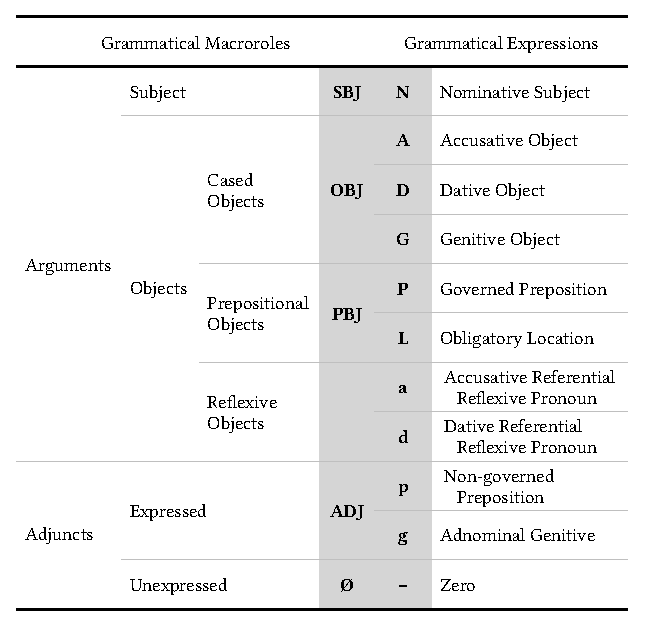
\includegraphics{figures/abbreviations.pdf}
\caption{Abbreviations used to describe role-remapping}\label{fig:abbreviations}
}
\end{figure}

Lower-cased\paragraphnumber{[2.40]} letters are used for non-argument
participants in the clause: `p' for non-governed prepositional phrases
and `g' for adnominal genitives. Adnominal genitives become relevant
because in some diatheses a newly introduced participant is inherently
the possessor of another participant (see
paragraph \hyperlink{par:possraising}{2.133} on page~\pageref{par:possraising}).
Absence of a specific role will be indicated by a dash. Lower-cased `a'
and `d' are only used in Sec­tion~\ref{sec:reflexive-no-diathesis} to
indicate accusative and dative reflexive pronouns in referential usage.
As described in much detail in that chapter, it is important to
distinguish between reflexive pronouns in German that refer to a lexical
role (i.e.~``referential'' or ``real'' reflexive constructions) and
reflexive pronouns that mark a diathesis without referring to a separate
role themselves. Only the former reflexive pronouns, those that are
(doubly) marking a role, are abbreviated by lowercased `a' or `d'.

Besides\paragraphnumber{[2.41]} single-letter abbreviations I will also
use capitalised three-letter abbreviations for a more abstract level of
analysis. As summarised at the left side of
Figure~\ref{fig:abbreviations}, the grammatical expressions are grouped
into sets of \textsc{grammatical macroroles}, mostly along familiar
lines. However, it is crucial to realise that these macroroles are
defined here as a superset of language-specific German grammatical
expressions. There is no abstract metalinguistic (universal) definition
assumed. The current grouping is not necessarily the best or most
optimal grouping, but this grouping has emerged to be useful to organise
the large diversity of diatheses in this book.

The\paragraphnumber{[2.42]} notion \textsc{subject (sbj)} is used for
nominative phrases that show agreement with the finite verb.\footnote{There
  are various other nominatively marked phrases in German grammar which
  are not included under this heading, e.g.~the nominative in nominal or
  equational predication like \emph{der Täter} in \emph{Er ist der
  Täter}.} The other case-marked governed phrases are combined as
\textsc{cased objects (obj)}. The cased objects together with the
\textsc{prepositional objects (pbj)} form a superclass of objects.
Non-governed phrases are separated in \textsc{overtly expressed adjuncts
(adj)} and unexpressed roles \textsc{omitted (ø)}. Although I will use
this five-way distinction throughout this book \textsc{(sbj, obj, pbj,
adj, ø)}, the five steps are not equidistant. The macroroles
\textsc{obj} and \textsc{pbj} are rather closely related, and likewise
are \textsc{adj} and \textsc{ø} intimately linked. Collapsing these
pairs results in the traditional subject-object-adjunct distinction.

\hypertarget{par:corecase}{
\paragraphnumber{[2.43]}\label{par:corecase}}There are some indications
that the group of cased objects \textsc{(obj)} might be fruitfully
separated into \textsc{core} (accusative) and \textsc{non-core}
(dative/genitive). This would simplify the analysis of case change in
object chains (Sec­tion~\ref{sec:intro-object-chains}), the antipassive
hierarchy (Sec­tion~\ref{sec:prepositions-demotion-of-object}) and the
case-marking of the reflexive pronoun
(Sec­tion~\ref{sec:reflexive-deponent}). However, in the majority of
diatheses all three cases seem to behave as a uniform group, so I did
not consistently pursue this separation.

It\paragraphnumber{[2.44]} is imperative to realise that the macroroles
are defined in a language-specific way for German grammar as groupings
of language-specific German expressions (e.g.~\textsc{adj} is defined as
being either a non-governed prepositional phrase or an adnominal
genitive). The names that are used (e.g.~``object'' or ``adjunct'')
deliberately conjure up general cross-linguistic associations, but it
remains to be seen whether similar definitions as used here are also
useful for other languages. I will refrain from any cross-linguistic
speculation in this context here.

\hypertarget{sec:intro-remapping}{%
\subsection{Remapping of roles}\label{sec:intro-remapping}}

All\paragraphnumber{[2.45]} diatheses in this book will be organised and
categorised in various levels of abstraction using the abbreviations as
summarised in Figure~\ref{fig:abbreviations}. The following levels of
abstraction will be used to arrange the diatheses in each chapter.

\textsc{level 1: diathesis}\paragraphnumber{[2.46]}. On the lowest
level, each diathesis is summarised in its own sub-subsection. The
establishment of an individual diathesis is not always obvious, and each
diathesis in this book is already a conscious categorisation (which
could be wrong). It has actually been a voyage of discovery in the
preparation of this book to decide when to consider a set of examples to
be a single diathesis. Very often erstwhile single diatheses turned out
to be better analysed by a separation into various different diatheses,
and vice versa. Although I am rather confident in the quality of the
current decisions, I expect that further refinements are necessary in
the future.

\textsc{level 2: remapping pattern}\paragraphnumber{[2.47]}. The
role-remapping of each diathesis is analysed using the single-letter
abbreviations (\textsc{nadgpl} pgad‑) from
Figure~\ref{fig:abbreviations}. A remapping is specified as an ordered
listing of grammatical expressions for roles, both before and after the
diathesis. For example, \textsc{{[}na\,\textbar\,‑n{]}} is a diathesis
that involves two roles that are marked N(ominative) and A(ccusative)
before the diathesis but unexpressed (``--'') and N(ominative) after the
diathesis, respectively. Because there are many diatheses with this same
pattern, this characterisation is already an (implicit) classification.

\textsc{level 3: local group}\paragraphnumber{[2.48]}. Groups of
diatheses with similar remapping and similar semantics within each
chapter can be grouped together as a local group. These groups are
rather ad-hoc and mainly represent a useful summary to streamline the
presentation. Local groups are indicated by similar names for the
diatheses.

\begin{sloppypar}
\textsc{level 4: macrorole pattern}\paragraphnumber{[2.49]}. The
remapping of each local group is structurally analysed in terms of the
three-letter macroroles \textsc{(sbj, obj, pbj, adj, ø)} from
Figure~\ref{fig:abbreviations}. For example, the remapping from above
\textsc{{[}na\,\textbar\,‑n{]}} includes both a change from \textsc{n}
to being omitted (i.e.~\textsc{sbj\,›\,ø}) and a change from \textsc{a}
to \textsc{n} (i.e.~\textsc{obj\,›\,sbj}). These two macrorole changes
can be combined into a single macrorole pattern
\textsc{obj\,›\,sbj\,›\,ø}.
\end{sloppypar}

\textsc{level 5: promotion/demotion}\paragraphnumber{[2.50]}. On the
most abstract level, all diatheses are separated into
chapter-subsections of either demotion or promotion (with only very few
diatheses being symmetrical exchanges). Basically, each remapping is
evaluated on the macrorole hierarchy (\ref{ex:macrorolehierarchy}) with
role-remapping upwards being promotion and role-remapping downward being
demotion. Note that there is a crucial additional criterion necessary,
because the majority of diatheses consist of chains of two coinciding
remappings (see Sec­tion~\ref{sec:intro-chaining} on the notion of
``chains''). In such chained remappings, the largest jump on the
macrorole hierarchy defines a diathesis as being demotion or promotion.
When both jumps are equally large, then the diathesis is
\textsc{symmetric}.\pagebreak

\ea \label{ex:macrorolehierarchy} Macrorole Hierarchy\\
  \textsc{sbj » obj » pbj » adj » ø}
\z

For\paragraphnumber{[2.51]} example, the diathesis in (\ref{ex2.30}) is
analysed as a \textsc{remapping pattern {[}na\,\textbar\,‑n{]}}, see
Sec­tion~\ref{sec:reflexive-anticausative}. This should be read as
follows: there is an alternation between a clause with \textsc{na}
arguments (nominative, accusative) and a clause with only \textsc{n}
marking (nominative). The relative order of these letters is crucial, as
the order of the roles remains fixed in this notation, e.g.~the second
letter on the left (\textsc{a} for accusative) corresponds to the second
letter on the right (\textsc{n} for nominative). The dash on the right
indicates that the corresponding \textsc{n} on the left is not
expressed. Note that the actual linear arrangement of the letters is
flexible, as long as both sides of the alternation remain in the same
order, i.e.~\textsc{{[}an\,\textbar\,n‑{]}} would be the same remapping
pattern as \textsc{{[}na\,\textbar\,‑n{]}}. The pattern
\textsc{{[}na\,\textbar\,‑n{]}} is an implicit categorisation, because
there are many other diatheses that have exactly the same pattern (see
e.g.
Sec­tions~\ref{sec:case-haben-anticausative}, \ref{sec:adverbial-reflexive-transitive-anticausative}, \ref{sec:participles-geben-reflexive-anticausative}).

\begin{samepage}
\ea \judgewidth{} \label{ex2.30} 
  \ea [] { Ich schließe die Tür. }
  \ex [] { Die Tür schließt sich. }
  \z
\z
\end{samepage}

Although\paragraphnumber{[2.52]} there is a reflexive pronoun in
(\ref{ex2.30}b), this pronoun is not included with a lower-cased `a' in
the remapping pattern \textsc{{[}na\,\textbar\,‑n{]}}, because this
reflexive pronoun does not refer to a separate role. The verb
\emph{schließen} `to close' implies at least two different roles, the
``closer'' and the ``closed object'', expressed as nominative and
accusative in (\ref{ex2.30}a), respectively. In (\ref{ex2.30}b) only the
role of ``closed object'' is expressed as nominative. The reflexive
pronoun does not refer to any other role. I interpret the reflexive
pronoun in (\ref{ex2.30}) as a marker of the diathesis itself (see
Chapter \ref{sec:reflexive} for an extensive discussion), so there is
actually an overt direction in the markedness from unmarked
(\ref{ex2.30}a) to reflexive-marked (\ref{ex2.30}b). The vertical bar
``\,\textbar\,'' in the middle of the remapping pattern
\textsc{{[}na\,\textbar\,‑n{]}} implies this direction in markedness
from left to right, i.e.~left side describes the unmarked alternant and
the right side the marked alternant. Reordering the remapping pattern
around the vertical bar would result in a completely reversed diathesis
\textsc{{[}‑n\,\textbar\,na{]}}.

The\paragraphnumber{[2.53]} diathesis in (\ref{ex2.30}) is one of
various examples of a \textsc{local group} that are all called
``reflexive antipassive''. Other diatheses in this group include
examples like (\ref{ex2.31}) with an additional governed preposition,
analysed here with the remapping pattern
\textsc{{[}nap\,\textbar\,‑np{]}}, see
Sec­tion~\ref{sec:reflexive-anticausative-governed-preposition}. All
diatheses in this local group have the same \textsc{macrorole pattern},
namely \textsc{obj\,›\,sbj\,›\,ø}, i.e a cased object is turned into
nominative subject, which is omitted (i.e.~unexpressed).\largerpage[2]

\ea \label{ex2.31} 
  \ea  Das Lied erinnert den Mann an den Krieg. 
  \ex  Der Mann erinnert sich an den Krieg. 
  \z
\z\pagebreak

\begin{sloppypar}
This\paragraphnumber{[2.54]} diathesis is a combination of two different
remappings \textsc{obj\,›\,sbj} and \textsc{sbj\,›\,ø}, with the first
being a promotion on the macrorole hierarchy and the second a demotion.
Crucially, because the demotion part \textsc{(sbj\,›\,ø)} is a larger
jump on the hierarchy than the promotion part \textsc{(obj\,›\,sbj)},
the complete combination is categorised as a \textsc{demotion}.
\end{sloppypar}

So,\paragraphnumber{[2.55]} in summary, the role-remapping of the
diathesis (\ref{ex2.31}) is categorised as summarised below. This
information also informs the place in the book where this diathesis will
be discussed: Reflexive voice is Chapter \ref{sec:reflexive}, demotion
that includes the subject in the macrorole pattern is always Section 5
within each chapter, and consequently, this diathesis can be found with
the heading \textsc{obj\,›\,sbj\,›\,ø} named ``reflexive antipassive''
in Sec­tion~\ref{sec:reflexive-anticausative-governed-preposition}.

\begin{enumerate}
\def\labelenumi{\arabic{enumi}.}

\item
  \textsc{diathesis}: reflexive antipassive+governed preposition
\item
  \textsc{remapping pattern}: \textsc{{[}nap\,\textbar\,‑np{]}}
\item
  \textsc{local group}: reflexive antipassive
\item
  \textsc{macrorole pattern}: \textsc{obj\,›\,sbj\,›\,ø}
\item
  \textsc{promotion/demotion}: demotion
\item
  \textsc{voice}: reflexive marking
\end{enumerate}

\hypertarget{sec:intro-stacking}{%
\section{Stacking}\label{sec:intro-stacking}}

\hypertarget{combining-diatheses}{%
\subsection{Combining diatheses}\label{combining-diatheses}}

Different\paragraphnumber{[2.56]} clause alternations (both diatheses
and epitheses) can be applied one after the other, forming
\textsc{stacks} of diatheses and/or epitheses. The term ``stacking'' is
introduced here explicitly in opposition to ``subordinating''.
Subordination leads to non-coherent multi-clause constructions, while
stacks always remain coherent and thus monoclausal. My impression is
that much of modern syntactic theory could be drastically simplified by
strictly distinguishing between stacking and subordinating.

Stacked\paragraphnumber{[2.57]} diatheses can lead to convoluted
role-remappings. A beautiful example of such stacking of diatheses is
given by Dixon (\citeyear*{dixon2014}: 252) for the
Amazonian language Paumarí. Here, the root \emph{noki‑} `to see' is
transparently related to the meaning `to show' through a series of
derivational diatheses, viz.~\emph{noki‑} `to see', \emph{noki-a‑} `to
be visible', \emph{na-noki-a‑} `to become visible', and finally
\emph{na-noki-a-hi‑} `to make become visible' i.e.~`to show'.

German\paragraphnumber{[2.58]} does not have that many morphologically
bound mechanisms for diathesis, though there are incidental examples
that come close. For example, the verb \emph{liegen} `to lie' changes
with ablaut to \emph{legen} `to lay' (see
Sec­tion~\ref{sec:case-umlaut-causative}), which in turn can take a
preverb to form \emph{be-legen} `to cover' (see
Sec­tion~\ref{sec:preverb-applicative-antipassive}). However, when the
perspective is broadened beyond bound morphology and all different kinds
of German diathesis are considered, then it turns out that stacking of
diatheses is extremely widespread.

In\paragraphnumber{[2.59]} many cases, the different steps in a stack
can be easily disentangled by carefully observing the formal marking of
the diathesis. For example, the construction in (\ref{ex9.57}c) includes
both a preverb \emph{be‑} and a reflexive pronoun \emph{sich} and it
turns out that these are applied in turn to make a stack of two
diatheses. Starting with the verb \emph{antworten} `to answer' with a
governed preposition \emph{auf} (\ref{ex2.32}a), the applicative preverb
\emph{be‑} changes the prepositional phrase to an accusative
(\ref{ex2.32}b), see Sec­tion~\ref{sec:preverb-applicative}.
Subsequently, the reflexive anticausative turns the accusative into a
nominative and drops the nominative agent (\ref{ex2.32}c), see
Sec­tion~\ref{sec:reflexive-anticausative}.

\begin{samepage}
\ea \judgewidth{} \label{ex2.32} 
  \ea [] { Der Lehrer antwortet auf deine Frage. }
  \ex [] { Der Lehrer beantwortet deine Frage. }
  \ex [] { Deine Frage beantwortet sich von selbst. }
  \z
\z
\end{samepage}

Clause\paragraphnumber{[2.60]} alternations are applied one after the
other, i.e.~the order of the alternations in a stack is of crucial
importance in most examples (unordered stacks exist, but are unusual,
see Sec­tion~\ref{sec:intro-disjunct-diatheses}). Basically, a stack is
just a list of clause alternations applied one after the other.
Syntactically this is just a linear sequence of application, i.e.~there
is no branching possible with stacking. Semantically this means that
each subsequent clause alternation has scope over the previous one.

A\paragraphnumber{[2.61]} stack can be written down using a symbol like
+\textgreater{} to indicate the additive (+) and sequential
(\textgreater) nature of the combination. The stack above (\ref{ex2.32})
can then be analysed as: (\ref{ex2.32}a) +\textgreater{} \emph{be‑}
applicative +\textgreater{} reflexive anticausative = (\ref{ex2.32}c).
This notation leads to concise analyses, as shown for example in
(\ref{ex9.60}) for the difference between the sentences
(\ref{ex2.33}a,b) and (\ref{ex2.33}c,d).

\begin{samepage}
\ea \judgewidth{} \label{ex2.33} 
  \ea [] { Der Lehrer hat die Aufgabe lösen wollen.\\
 }
  \ex [] { Basic clause: Der Lehrer löst die Aufgabe.\\
+\textgreater{} \emph{wollen} modal (cf. \ref{sec:infinitive-modals})\\
\hspace*{0.333em}\hspace*{0.333em}\hspace*{0.333em}\hspace*{0.333em}=
Der Lehrer will die Aufgabe lösen.\\
+\textgreater{} \emph{haben} perfect (cf.
\ref{sec:participles-haben-perfect})\\
\hspace*{0.333em}\hspace*{0.333em}\hspace*{0.333em}\hspace*{0.333em}=
Der Lehrer hat die Aufgabe lösen wollen.\\
 }
  \ex [] { Der Lehrer will die Aufgabe gelöst haben.\\
 }
  \ex [] { Basic clause: Jemand löst die Aufgabe für den Lehrer.\\
+\textgreater{} beneficiary dative (cf.
\ref{sec:prepositions-benefactive-dative})\\
\hspace*{0.333em}\hspace*{0.333em}\hspace*{0.333em}\hspace*{0.333em}=
Jemand löst dem Lehrer die Aufgabe.\\
+\textgreater{} \emph{haben} dative passive (cf.
\ref{sec:participles-haben-passive})\\
\hspace*{0.333em}\hspace*{0.333em}\hspace*{0.333em}\hspace*{0.333em}=
Der Lehrer hat die Aufgabe gelöst.\\
+\textgreater{} \emph{wollen} modal (cf. \ref{sec:infinitive-modals})\\
\hspace*{0.333em}\hspace*{0.333em}\hspace*{0.333em}\hspace*{0.333em}=
Der Lehrer will die Aufgabe gelöst haben. }
  \z
\z
\end{samepage}

With\paragraphnumber{[2.62]} unmarked (``covert'') diatheses such stacks
can sometimes be tricky to tease apart. As an example, consider the
arguably somewhat artificially constructed example in (\ref{ex2.34})
using the verb \emph{schneiden} `to cut'. It starts off in
(\ref{ex2.34}a) as a basic transitive construction with a nominative and
accusative argument. Yet, after various twists and turns it ends up on
(\ref{ex2.34}f) with a nominative, an accusative, a dative and an
obligatory location prepositional phrase, while the original agent
\emph{Arzt} is not even expressed.

\begin{samepage}
\ea \judgewidth{} \label{ex2.34} 
  \ea [] { Der Arzt schneidet den Nagel des Patienten. }
  \ex [] { Der Arzt schneidet in den Nagel des Patienten. }
  \ex [] { Der Arzt schneidet dem Patienten in den Nagel. }
  \ex [] { Der Arzt schneidet dem Patienten einen Schlitz in den
Nagel. }
  \ex [] { Der Arzt schneidet dem Patienten einen Schlitz in den Nagel
mit dem Fräser. }
  \ex [] { Der Fräser schneidet dem Patienten einen Schlitz in den
Nagel. }
  \z
\z
\end{samepage}

Teasing\paragraphnumber{[2.63]} this stack apart, there are five
different diatheses, concurrently showing that the verb \emph{schneiden}
has at least five different lexeme-specific roles. As defined in
Sec­tion~\ref{sec:intro-arguments-utterance-valency}, each role that
appears as a case-marked constituent in at least one diathesis is a
lexeme-specific role, and all of the following participants are
case-marked in the stack of diatheses (\ref{ex2.34}):

\begin{itemize}
\item
  the cutter \emph{Arzt} `physician'
\item
  the cut object \emph{Nagel} `nail'
\item
  the possessor of the cut object \emph{Patient} `patient'
\item
  the result of the cutting \emph{Schlitz} `groove, slit'
\item
  the instrument doing the cutting \emph{Fräser} `milling cutter'
\end{itemize}

The\paragraphnumber{[2.64]} five diatheses (and the corresponding
role-remappings) are the following:

\begin{itemize}
\item
  (\ref{ex2.34}b), \emph{in} antipassive: changing the cut object
  \emph{Nagel} from accusative to prepositional object, see
  Sec­tion~\ref{sec:prepositions-in-antipassive}.
\item
  (\ref{ex2.34}c), possessor raising: changing the possessor of the cut
  object \emph{Patient} from adnominal genitive into dative, see
  Sec­tion~\ref{sec:prepositions-possessor-of-location-to-dative-experiencer}.
\item
  (\ref{ex2.34}d), object exchange: adding a new accusative object
  \emph{Schlitz} as the result of the cutting, see
  Sec­tion~\ref{sec:prepositions-partitive-free}.
\item
  (\ref{ex2.34}e), adjunct addition: adding a syntacticaly optional
  instrument \emph{Fräser}, see
  Sec­tion~\ref{sec:prepositions-comitative-intrumental}.
\item
  (\ref{ex2.34}f), instrument anticausative: turning the instrument
  \emph{Fräser} from prepositional phrase to nominative, see
  Sec­tion~\ref{sec:prepositions-transitive-conciliative}.
\end{itemize}

\hypertarget{fixed-stacks}{%
\subsection{Fixed stacks}\label{fixed-stacks}}

There\paragraphnumber{[2.65]} are a few examples of diatheses that look
like stacks of two diatheses, but on closer inspection it turns out that
the intermediate construction does not exist. A few major examples of
such \textsc{fixed stacks} are exemplified below.

There\paragraphnumber{[2.66]} is an infamous anticausative diathesis
that needs a reflexive pronoun, which is attested for a large, but
restricted group of verbs like \emph{schließen} `to close'
(\ref{ex2.35}a,b), see Sec­tion~\ref{sec:reflexive-anticausative}. A
completely different group of verbs also has an anticausative diathesis
with a reflexive pronoun, but only with an additional evaluative
adverbial. This is for example attested with \emph{verkaufen} `to sell'
(\ref{ex2.35}c,d), see
Sec­tion~\ref{sec:adverbial-reflexive-transitive-anticausative}. In this
case, the diathesis is marked by both the reflexive pronoun and the
presence of an adverbial, and neither is possible without the other.
Such a combination of two obligatorily co-occurring formal marking
strategies is called a \textsc{fixed stack}.

\begin{samepage}
\ea \judgewidth{} \label{ex2.35} 
  \ea [] { Ich schließe die Tür. }
  \ex [] { Die Tür schließt sich. }
  \ex [] { Ich verkaufe das Buch. }
  \ex [] { Das Buch verkauft sich gut. }
  \z
\z
\end{samepage}

Various\paragraphnumber{[2.67]} diatheses between a verb, like
\emph{fassen} `to grasp' (\ref{ex2.36}a), and its pre­verb-alternant,
like \emph{befassen} `to be concerned with' (\ref{ex2.36}b),
additionally need a reflexive pronoun, see
Sec­tion~\ref{sec:preverb-reflexive-antipassive}. So here we have a fixed
stack of a reflexive pronoun and a preverb together that mark the
diathesis.

\begin{samepage}
\ea \judgewidth{} \label{ex2.36} 
  \ea [] { Ich fasse einen Entschluss. }
  \ex [] { Ich befasse mich mit dem Entschluss. }
  \z
\z
\end{samepage}

Also\paragraphnumber{[2.68]} some light verb alternations show fixed
stacks. For example, there is a very widespread causative diathesis
using the light verb \emph{lassen} with an infinitive (\ref{ex2.37}b),
see Sec­tion~\ref{sec:infinitive-lassen-causative}. Additionally, the
combination of \emph{lassen+In­fi­ni­tiv} and a reflexive pronoun leads to
a passive alternation (\ref{ex2.37}c), which does not make sense as
being derived from the causative (\ref{ex2.37}b). It seems better to
consider the combination of \emph{lassen+Infinitiv+Reflexiv} as a fixed
stack, see Sec­tion~\ref{sec:infinitive-lassen-reflexive-passive}.

\begin{samepage}
\ea \judgewidth{} \label{ex2.37} 
  \ea [] { Der Schüler löst die Aufgabe. }
  \ex [] { Der Lehrer lässt den Schüler die Aufgabe lösen. }
  \ex [] { Diese Aufgabe lässt sich (von den Schülern) lösen. }
  \z
\z
\end{samepage}

\hypertarget{sec:intro-chaining}{%
\section{Chaining}\label{sec:intro-chaining}}

\hypertarget{beyond-solitary-remapping}{%
\subsection{Beyond solitary remapping}\label{beyond-solitary-remapping}}

Many\paragraphnumber{[2.69]} diatheses just remap a single role. Such
diatheses are called \textsc{isolated diatheses} here. However, there
are also many diatheses in which more than one role is remapped. I
distinguish the following kinds of combined role-remappings, of which
only the first is frequently attested.

\begin{itemize}
\tightlist
\item
  \textsc{chained diathesis}
  (Sec­tion~\ref{sec:intro-chained-diatheses}): Two roles change their
  formal marking, forming a chain in which one role changes its form
  from X to Y, while the other role changes its form from Y to Z. This
  results in a chain \textsc{(x\,›\,y\,›\,z)}.
\item
  \textsc{multi-chained diathesis}
  (Sec­tion~\ref{sec:intro-multi-chained-diatheses}): Three (or possibly
  even more) roles change their formal marking, forming a longer chain
  of connected changes.
\item
  \textsc{disjunct diathesis}
  (Sec­tion~\ref{sec:intro-disjunct-diatheses}): Two or more roles change
  their formal marking, with no overlap between marking.
\end{itemize}

Chained\paragraphnumber{[2.70]} diatheses are surprisingly frequent in
German, and my impression is that this pervasiveness extends to many
other languages beyond German. In a chained diathesis the result of the
first remapping is the start of the second remapping. This can be
conceptualised as a ``push'' or ``pull'' chain in which one remapping
induces another. The prevalence of such chains is probably caused by two
general tendencies of language structure, namely \textsc{distinctness}
and \textsc{default marking}. These tendencies are formulated here as
hypotheses for language structure in general, beyond the specifics of
German.

First,\paragraphnumber{[2.71]} the tendency for distinctness causes
language to disprefer multiple constituents with the same structure in a
single clause. For example, the German languages tends to prevent two
accusatives in the same clause. In effect, if a diathesis would gives
rise to such a duplication, then the duplicated constituent is
preferably ``pushed'' out to another kind of marking. Second, the
principle of default marking induces languages to mark at least one of
its constituents as the ``default'' in each clause. For example, in
German the nominative subject has to be present in almost every clause.
As a result, if a diathesis removes this preferred constituent, then
another constituent is typically ``pulled'' into this kind of marking.
It remains to be further investigated whether these two forces really
exist, and whether the two tendencies can be teased apart.

\hypertarget{sec:intro-chained-diatheses}{%
\subsection{Chained diatheses}\label{sec:intro-chained-diatheses}}

In\paragraphnumber{[2.72]} German, chained diatheses typically occur
when the nominative subject is involved in the diathesis. There can only
be a single nominative subject in a German clause, and it is highly
unusual to have a sentence without a nominative subject. This implies
that any diathesis involving the nominative subject typically includes
two remappings, namely one from something else to nominative and a
second remapping of the erstwhile nominative to something else.

A\paragraphnumber{[2.73]} prototypical example of a chained diathesis
involving the nominative subject is the \emph{werden} passive
(\ref{ex2.38}). Here, the erstwhile accusative \emph{Kuchen} `cake' is
turned into a nominative, while the erstwhile nominative \emph{Lehrling}
`apprentice' is removed (or optionally retained as a \emph{von}
prepositional phrase). So, we have a chain consisting of the
role-remappings \textsc{obj\,›\,sbj} and \textsc{sbj\,›\,adj}.

\begin{samepage}
\ea \judgewidth{} \label{ex2.38} \textsc{chained diathesis
(obj\,›\,sbj\,›\,adj)}
  \ea [] { Der Lehrling backt den Kuchen. }
  \ex [] { Der Kuchen wird gebacken (von dem Lehrling). }
  \z
\z
\end{samepage}

Diatheses\paragraphnumber{[2.74]} without involvement of the nominative
subject are more flexible, in that both isolated and chained diatheses
are common. A typical example of a chained diathesis is an object
exchange induced by the preverb \emph{be‑} (\ref{ex2.39}). In this
example, a prepositional phrase \emph{für ihre Freundin} `for her
friend' is remapped to an accusative \textsc{(adj\,›\,obj)} while the
erstwhile accusative \emph{Essen} `food' is turned into a prepositional
phrase \textsc{(obj\,›\,adj)}.

\begin{samepage}
\ea \judgewidth{} \label{ex2.39} \textsc{chained diathesis
(adj\,›\,obj\,›\,adj)}
  \ea [] { Sie kocht kubanisches Essen für ihre Freundin. }
  \ex [] { Sie bekocht ihre Freundin mit kubanischem Essen. }
  \z
\z
\end{samepage}

Among\paragraphnumber{[2.75]} the chained diatheses there is a group of
frequently recurring remapping patterns. Because of their frequency, it
is highly useful to give them specific names. Such names are widespread
in the literature, e.g.~anticausative for \textsc{obj\,›\,sbj\,›\,ø} or
passive for \textsc{obj\,›\,sbj\,›\,adj}. A survey of the various names
used in this book will be pursued in Sec­tion~\ref{sec:intro-naming}.

\hypertarget{sec:intro-multi-chained-diatheses}{%
\subsection{Multi-chained
diatheses}\label{sec:intro-multi-chained-diatheses}}

\textsc{multi-chained diatheses}\paragraphnumber{[2.76]} consist of
combinations of more than two role-re­map­pings that occur in a sequence.
This occurs frequently as the result of a stack of multiple diatheses,
but only very rarely in a single diathesis. As an example arising from a
stack of multiple diatheses consider taking a verb like \emph{lesen} `to
read' (\ref{ex2.40}a) and applying a stack of two diatheses
(\ref{ex2.40}b,c). This leads to a chain of three role-remappings.
First, the preverb diathesis with \emph{vor‑} (\ref{ex2.40}b) leads to
the addition of a dative argument \emph{dem Jungen}, i.e.~a
role-remapping \textsc{ø\,›\,obj}, see
Sec­tion~\ref{sec:preverb-dative-addition-accusative}. On top of that,
the \emph{bekommen} dative passive (\ref{ex2.40}c) promotes this dative
to subject and removes the original subject, i.e.~a role-remapping
\textsc{obj\,›\,sbj\,›\,ø}, see
Sec­tion~\ref{sec:participles-bekommen-passive}. Combined, these two
diatheses lead to a multi-chained role-re­map­ping
\textsc{ø\,›\,obj\,›\,sbj\,›\,ø}.

\begin{samepage}
\ea \judgewidth{} \label{ex2.40} \textsc{multi-chained diathesis
(ø\,›\,obj\,›\,sbj\,›\,ø)}
  \ea [] { Der Vater hat ein Buch gelesen. }
  \ex [] { Der Vater hat dem Jungen ein Buch vorgelesen. }
  \ex [] { Der Junge bekommt ein Buch vorgelesen. }
  \z
\z
\end{samepage}

Such\paragraphnumber{[2.77]} multi-chained diatheses that are the result
of diathesis-stacking are widespread. However, I know of only two
diatheses with a multi-chain that cannot be decomposed into a stack of
separate diatheses. Both these ``fixed'' multi-chain diatheses appear to
occur with just a few idiosyncratic verbs, so this phenomenon really
seems to be dispreferred in German.

First,\paragraphnumber{[2.78]} the preverb diathesis from \emph{erben}
`to inherit' to \emph{enterben} `to disinherit' (\ref{ex2.41}), see
Sec­tion~\ref{sec:preverb-inverted-passive-accusative-loss}, contains
three linked role-remappings for (i) the originator of the inheritance
\emph{Vater} `father' \textsc{(adj\,›\,sbj)}, (ii) the receiver of the
inheritance \emph{Junge} `boy' \textsc{(sbj\,›\,obj)} and (iii) the
inheritance \emph{Schreibtisch} `desk' \textsc{(obj\,›\,ø)}.

\begin{samepage}
\ea \judgewidth{} \label{ex2.41} \textsc{multi-chained diathesis
(adj\,›\,sbj\,›\,obj\,›\,ø)}
  \ea [] { Der Junge erbt den Schreibtisch von seinem Vater. }
  \ex [] { Sein Vater enterbt den Jungen. }
  \z
\z
\end{samepage}

Second,\paragraphnumber{[2.79]} the verb \emph{schmecken} `to taste'
(\ref{ex10.77}), see
Sec­tion~\ref{sec:prepositions-ingredient-anticausative}, allows for two
different constructions with three linked role-remappings for (i) the
tasted substance \emph{Pfefferminze} `peppermint'
\textsc{(obj\,›\,adj)}, for (ii) the tasted dish \emph{Suppe} `soup'
\textsc{(adj\,›\,sbj)} and for (iii) the taster \emph{Koch} `cook'
\textsc{(sbj\,›\,ø)}.

\begin{samepage}
\ea \judgewidth{} \label{ex2.42} \textsc{multi-chained diathesis
(obj\,›\,adj\,›\,sbj\,›\,ø)}
  \ea [] { Der Koch schmeckt die Pfefferminze in der Suppe. }
  \ex [] { Die Suppe schmeckt nach Pfefferminze. }
  \z
\z
\end{samepage}

\hypertarget{sec:intro-disjunct-diatheses}{%
\subsection{Disjunct diatheses}\label{sec:intro-disjunct-diatheses}}

\textsc{disjunct diatheses}\paragraphnumber{[2.80]} consist of a
combination of multiple role-remappings that are not linked to each
other. Just as with the multi-chained diatheses from the previous
section, disjunct diatheses regularly occur as the result of stacking of
diatheses. In contrast, they are very rare in individual diatheses.

When\paragraphnumber{[2.81]} multiple diatheses are stacked, i.e.~when
they are applied sequentially on top of each other, they are sometimes
structurally independent (and thus unordered). For example, the verb
\emph{waschen} `to wash' (\ref{ex2.43}a) can be used in a
object-exchange diathesis (\ref{ex2.43}b) in which the role of washee
\emph{Hemd} `shirt' is turned from an accusative into a location
\textsc{(obj\,›\,pbj)} and a new accusative object is introduced for the
role of the object to be removed \emph{Fleck} `stain'
\textsc{(ø\,›\,obj)}, see Sec­tion~\ref{sec:prepositions-partitive-free}.
Independent of this chained diathesis, the possessor of the object
\emph{Nachbar} `neighbour' can be raised to genitive (\ref{ex2.43}c),
i.e.~a possessor applicative \textsc{(adj\,›\,obj)}, see
Sec­tion~\ref{sec:prepositions-possessor-of-location-to-dative-experiencer-accusative}.

\begin{samepage}
\ea \judgewidth{} \label{ex2.43} \textsc{disjunct diathesis
(ø\,›\,obj\,›\,pbj + adj\,›\,obj)}
  \ea [] { Ich wasche das Hemd des Nachbarn. }
  \ex [] { Ich wasche den Fleck aus dem Hemd des Nachbarn. }
  \ex [] { Ich wasche dem Nachbarn den Fleck aus dem Hemd. }
  \z
\z
\end{samepage}

There\paragraphnumber{[2.82]} are only a few incidental examples of such
disjunct diatheses without stacking. The following four examples all
only occur with a very limited number of verbs. First, the verb
\emph{deuten} can be used both to mean `interpret' (\ref{ex2.44}a) and
`forebode' (\ref{ex2.44}b) with a rather transparent connection between
the two. However, the role-remappings are quite complex, see
Sec­tion~\ref{sec:prepositions-anticausative-preposition-addition}.

\begin{samepage}
\ea \judgewidth{} \label{ex2.44} \textsc{disjunct diathesis (ø\,›\,pbj +
obj\,›\,sbj\,›\,ø)}
  \ea [] { Ich deute den Traum. }
  \ex [] { Der Traum deutet auf nichts Gutes. }
  \z
\z
\end{samepage}

Second,\paragraphnumber{[2.83]} some preverbs lead to disjunct
diatheses, like with \emph{schweigen} `to remain silent' and
\emph{verschweigen} `to conceal' (\ref{ex2.45}), see
Sec­tion~\ref{sec:preverb-double-applicative}.

\begin{samepage}
\ea \judgewidth{} \label{ex2.45} \textsc{disjunct diathesis (adj\,›\,obj
+ pbj\,›\,obj)}
  \ea [] { Ich schweige zu dir über meinen Besuch. }
  \ex [] { Ich verschweige dir meinen Besuch. }
  \z
\z
\end{samepage}

Further\paragraphnumber{[2.84]} examples are a few verbs of naming like
\emph{schimpfen} `to scold' (\ref{ex2.46}), see
Sec­tion~\ref{sec:prepositions-naming-result}. The disjunct diathesis in
(\ref{ex2.47}) is less clear, as it might be better analysed as a stack,
see Sec­tion~\ref{sec:prepositions-nominative-demotion-dative-addition}.

\begin{samepage}
\ea \judgewidth{} \label{ex2.46} \textsc{disjunct diathesis (ø\,›\,obj +
adj\,›\,obj)}
  \ea [] { Sie schimpft auf mich. }
  \ex [] { Sie schimpft mich einen Narren }
  \z
\z
\end{samepage}

\begin{samepage}
\ea \judgewidth{} \label{ex2.47} \textsc{disjunct diathesis (ø\,›\,obj +
sbj\,›\,adj)}
  \ea [] { Der Sommer ist kalt. }
  \ex [] { Mir ist kalt im Sommer. }
  \z
\z
\end{samepage}

The\paragraphnumber{[2.85]} only more widespread disjunct diathesis is
the caused-motion construction that can arise with some apparently
intransitive verbs like \emph{schwitzen} `to sweat' (\ref{ex2.48}). This
diathesis introduces two roles at once: a result of the sweating
\emph{Fleck} `stain' and an obligatory location of the result
\emph{Hemd} `shirt', see
Sec­tion~\ref{sec:prepositions-intransitive-location-as-result}.

\begin{samepage}
\ea \judgewidth{} \label{ex2.48} \textsc{disjunct diathesis (ø\,›\,obj +
ø\,›\,pbj)}
  \ea [] { Ich schwitze. }
  \ex [] { Ich schwitze einen Fleck in mein Hemd. }
  \z
\z
\end{samepage}

\hypertarget{sec:intro-naming}{%
\section{Naming}\label{sec:intro-naming}}

\hypertarget{names-for-macrorole-patterns}{%
\subsection{Names for macrorole
patterns}\label{names-for-macrorole-patterns}}

Throughout\paragraphnumber{[2.86]} the introductory chapters I have used
various names for diatheses, like passive, antipassive, applicative or
causative. These names have a long history in the typological
grammatical literature (cf. \citealt{melcuk1993}; \citealt{wunderlich1993};
\citealt{wunderlich2015};
\citealt{dixon2000a};
\citealt{dixon2014};
\citealt{haspelmath2004c}; \citealt{kulikov2011};
\citealt{malchukov2015}: 96ff.;
\citealt{zuniga2019}). Although I
have been using these terms as if their meaning is clear, this is often
far from the truth. Many different terms and definitions have been
proposed in the literature, and different terms have at times been used
for the same phenomena. For example, the original proposal for the term
``antipassive'' is already 50 years old
(\citealt{silverstein1972}: 395), but
the same phenomenon is also known as deaccusative
(\citealt{geniusiene1987}: 94) or
antiapplicative (\citealt{haspelmath2004c}: 1132; \citealt{scheibl2006}: 371). 
Conversely, the term antipassive is also attested referring
to a slightly different phenomenon of the drop of an object
(\citealt{scheibl2006}: 372--373).

In\paragraphnumber{[2.87]} this section I will describe in more detail
how these names are used and defined in the current book about German
diatheses. The names for diatheses will here always refer to a macrorole
pattern, i.e.~to the highly abstract classification of a diathesis in
terms of \textsc{sbj}, \textsc{obj}, etc. as defined in
Sec­tion~\ref{sec:intro-remapping}. For example, the term
``anticausative'' will be used as a name for the macrorole pattern
\textsc{obj\,›\,sbj\,›\,ø}. Such macrorole patterns are strictly defined
here in a language-specific way for German, so care should be taken when
applying the same names to different languages.

One\paragraphnumber{[2.88]} widespread term that I will avoid is the
term ``middle'' (and likewise the Latinate equivalent term ``medium'').
This term for a diathesis is already attested as \emph{μεσότης} in the
oldest known Greek grammatical text, the \emph{τέχνη γραμματική} of
Dionysius Thrax, and it has become a mainstay in the grammatical
literature ever since.\footnote{Thrax writes: \emph{διαθέσεις εἰσὶ
  τρεῖς, ἐνέργεια, πάθος, μεσότης} `there are three diatheses, active,
  passive and middle' (\citealt{uhlig1883}: 48).} 
The phenomena that are called ``middle'' in the literature are
highly variable, and there is no consensus about what kind of diathesis
this term is supposed to designate, other than something that is neither
active nor passive (see \citealt{zuniga2019}: 168--177 for a thorough summary 
of the complex
philological history of the term middle/medium). Such a broad and
ill-defined term is not useful for a detailed analysis of the large
variety of attested role-remappings in German.

The\paragraphnumber{[2.89]} discussion about the different names for
macrorole patterns will be split into four parts. First, the next two
sections will present names for diatheses involving the nominative
subject. Subsequent sections will discuss diatheses not involving the
subject. In both discussions, a central distinction will be made between
isolated diatheses and chained diatheses (cf.
Sec­tion~\ref{sec:intro-chaining}).

\hypertarget{sec:intro-isolated-subject-diathesis}{%
\subsection{Isolated subject
diatheses}\label{sec:intro-isolated-subject-diathesis}}

\hypertarget{par:insubjective}{
\paragraphnumber{[2.90]}\label{par:insubjective}}Isolated diatheses that
involve a nominative subject do not show much variation in German. The
most widespread kind is the drop of the subject \textsc{(sbj\,›\,ø)},
i.e.~the complete removal of the role marked as nominative subject
without any further accompanying role-remapping or reintroduction of a
new subject. This is typically attested with intransitive verbs: after
removing the single available role, there is no other role introduced to
fill the structural subject position. Semantically, such diatheses put
the focus on the activity as described by the verb itself, so I propose
to call them \textsc{insubjective} diatheses. Note that there is a
strong tendency for every German sentence to formally have a nominative
subject with verb agreement. Consequently, such insubjective diatheses
regularly (but not always) result in the presence of a
valency-simulating nominative pronoun \emph{es} (see
Sec­tion~\ref{sec:intro-es}).

An\paragraphnumber{[2.91]} \textsc{insubjective} diathesis is attested
with verbs like \emph{stinken} `to stink' (\ref{ex2.49}), see
Sec­tion~\ref{sec:case-nominative-drop}. In a sentence like \emph{es
stinkt} the pronoun \emph{es} can of course simply be an anaphor, like
in (\ref{ex2.49}b). In such a sentence, the role of ``stinker'' is still
present and there is no diathesis at all. However, in other contexts
(\ref{ex2.49}c) the verb \emph{stinken} is used without implied subject.
This is typically attested in contexts in which some odour is attested,
but the originator is not known.

\begin{samepage}
\ea \judgewidth{} \label{ex2.49} \textsc{insubjective (sbj\,›\,ø)}
  \ea [] { Der Müll stinkt. }
  \ex [] { Das schmutzige Tuch, es stinkt! }
  \ex [] { Hier stinkt es. }
  \z
\z
\end{samepage}

Another\paragraphnumber{[2.92]} example of a insubjective diathesis is
illustrated with the verb \emph{leben} `to live' (\ref{ex2.50}), see
Sec­tion~\ref{sec:adverbial-reflexive-drop}. Many such intransitive verbs
can be used without a subject in a habitual sense, but this is only
possible with an obligatory adverbial qualification like \emph{gut}
(\ref{ex2.50}b,c).

\begin{samepage}
\ea \judgewidth{*} \label{ex2.50} \textsc{insubjective (sbj\,›\,ø)}
  \ea [] { Ich lebe in diesem Haus. }
  \ex [] { In diesem Haus lebt es sich gut. }
  \ex [*] { In diesem Haus lebt es sich. }
  \z
\z
\end{samepage}

Also\paragraphnumber{[2.93]} the so-called impersonal passive consisting
of \emph{werden+Partizip} (\ref{ex2.51}), see
Sec­tion~\ref{sec:participles-werden-impersonal-passive}, is an example
of a insubjective diathesis, in this case even without any
valency-simulating \emph{es}.

\begin{samepage}
\ea \judgewidth{*} \label{ex2.51} \textsc{insubjective (sbj\,›\,ø)}
  \ea [] { Die Jungs tanzen hier. }
  \ex [] { Hier wird getanzt. }
  \ex [*] { Hier wird es getanzt. }
  \z
\z
\end{samepage}

\hypertarget{par:desubjective}{
\paragraphnumber{[2.94]}\label{par:desubjective}}A different kind of
isolated subject diathesis is subject demotion of the nominative subject
to a prepositional phrase. An example is the \emph{geben+zu‑In­fi­ni­tiv}
(\ref{ex2.52}), see Sec­tion~\ref{sec:zuinfinitive-geben-demotion}. In
this diathesis, the subject is demoted to an optional non-governed
prepositional phrase \textsc{(sbj\,›\,adj)}. The demotion is the only
role-remapping that is happening in this diathesis, so I propose to call
such a diathesis a \textsc{desubjective}.

\begin{samepage}
\ea \judgewidth{} \label{ex2.52} \textsc{desubjective (sbj\,›\,adj)}
  \ea [] { Wir gewinnen einen Preis. }
  \ex [] { es gibt (für uns) einen Preis zu gewinnen. }
  \z
\z
\end{samepage}

The\paragraphnumber{[2.95]} other isolated subject diatheses are only
attested in incidental examples in German, like a subject demotion to a
governed preposition \textsc{(sbj\,›\,pbj)} with \emph{fehlen} shown in
(\ref{ex2.53}), see Sec­tion~\ref{sec:prepositions-nominative-demotion}.

\begin{samepage}
\ea \judgewidth{} \label{ex2.53} \textsc{desubjective (sbj\,›\,pbj)}
  \ea [] { Das Geld fehlt ihm. }
  \ex [] { Ihm fehlt es an Geld. }
  \z
\z
\end{samepage}

Isolated\paragraphnumber{[2.96]} \textsc{subject addition (ø\,›\,sbj)}
is very rare in German, partly because it would need an unmarked
construction without any subject to start off with. A possible example
is the addition of a subject that seems possible with some weather verbs
like \emph{donnern} `to thunder' (\ref{ex2.54}), see
Sec­tion~\ref{sec:case-nominative-addition}.\largerpage

\begin{samepage}
\ea \judgewidth{} \label{ex2.54} \textsc{subject addition (ø\,›\,sbj)}
  \ea [] { Es donnert. }
  \ex [] { Die Motoren donnerten. }
  \z
\z
\end{samepage}

\hypertarget{chained-subject-diatheses}{%
\subsection{Chained subject diatheses}\label{chained-subject-diatheses}}

Chained\paragraphnumber{[2.97]} diatheses that involve the nominative
subject are widespread in German (in contrast to the infrequent
occurrence of isolated diatheses as discussed previously).
Figure~\ref{fig:subjectchains} presents an overview of the different
terms that I will use for these diatheses. The bold-faced terms are used
for widely attested diatheses, while the other kinds of diatheses are
only incidentally found. There is currently no evidence in German for
the existence of the remappings that are left empty in the figure. There
appears to be a preference for various kinds of demotion (i.e.~the upper
right corner of the figure), which fits nicely with the known
typological preference of German for anticausative constructions
(\citealt{haspelmath1993a}: 101;
\citealt{nichols2004}:
189).

\begin{figure}
\hypertarget{fig:subjectchains}{%
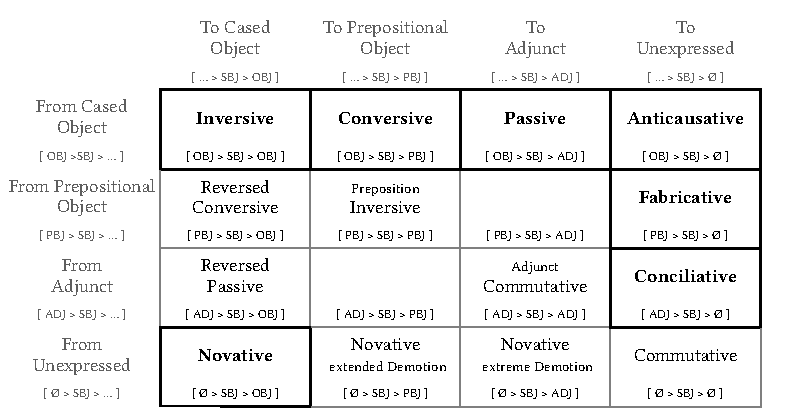
\includegraphics[width=\textwidth]{figures/subjectchains.pdf}
\caption{Names for chained macro-role remappings with the subject in the
middle of the chain}\label{fig:subjectchains}}
\end{figure}

The\paragraphnumber{[2.98]} upper right part of
Figure~\ref{fig:subjectchains} are demotions, the lower left part are
promotions, and on the diagonal are examples of symmetrical diatheses. I
will discuss all types in this order.\largerpage

\hypertarget{sec:intro-subject-demotions}{%
\subsubsection{Demotions}\label{sec:intro-subject-demotions}}

\hypertarget{par:anticausative}{
\paragraphnumber{[2.99]}\label{par:anticausative}}The most extreme kind
of demotion is an \textsc{anticausative (obj\,›\,sbj\,›\,ø)}. The
typical characteristic of an anticausative is the complete removal of
the nominative subject that is the causer of the action/state of the
clause. Filling the syntactic gap, a case-marked argument (typically the
accusative) is promoted to subject. This is a widespread kind of
diathesis. An example is the reflexive anticausative with verb like
\emph{schliessen} `to close' (\ref{ex2.55}), see
Sec­tion~\ref{sec:reflexive-anticausative}.

\begin{samepage}
\ea \judgewidth{} \label{ex2.55} \textsc{anticausative
(obj\,›\,sbj\,›\,ø)}
  \ea [] { Ich schließe die Tür. }
  \ex [] { Die Tür schließt sich (von alleine). }
  \z
\z
\end{samepage}

\hypertarget{par:passive}{
\paragraphnumber{[2.100]}\label{par:passive}}Very similar to an
anticausative is the \textsc{passive (obj\,›\,sbj\,›\,adj)}. The main
difference between the two (a distinction which is often difficult to
delimit) is that for a passive the original subject is still implied and
can optionally be overtly expressed (\ref{ex2.56}). In contrast, for an
anticausative the original subject is completely removed and a phrase
like \emph{by itself} can typically be added. As an example of a passive
diathesis in (\ref{ex2.56}) is the \emph{bekommen Rezipientenpassiv} in
which a dative is promoted to subject
Sec­tion~\ref{sec:participles-bekommen-passive}

\begin{samepage}
\ea \judgewidth{} \label{ex2.56} \textsc{passive (obj\,›\,sbj\,›\,adj)}
  \ea [] { Ihr Freund kocht ihr eine Suppe. }
  \ex [] { Sie bekommt von ihrem Freund eine Suppe gekocht. }
  \z
\z
\end{samepage}

\hypertarget{par:conversive}{
\paragraphnumber{[2.101]}\label{par:conversive}}A \textsc{conversive
(obj\,›\,sbj\,›\,pbj)} looks similar to a passive, except that the
prepositional phrase is a lexically governed preposition, so it has a
more object-like grammatical status. An example is the verb
\emph{empören} `to appall' (\ref{ex2.57}a) with the reflexive diathesis
\emph{sich empören über} `to be outraged about' (\ref{ex2.57}b,c), see
Sec­tion~\ref{sec:reflexive-preposition-passive}. The term conversive is
adapted from Kulikov (\citeyear*{kulikov2011}: 380).

\begin{samepage}
\ea \judgewidth{} \label{ex2.57} \textsc{conversive
(obj\,›\,sbj\,›\,pbj)}
  \ea [] { Der Preis empört den Kunden. }
  \ex [] { Der Kunde empört sich über den Preis. }
  \ex [] { Der Kunde empört sich darüber, dass der Preis schon wieder
gestiegen ist. }
  \z
\z
\end{samepage}

\hypertarget{par:fabricative}{
\paragraphnumber{[2.102]}\label{par:fabricative}}For the next diathesis,
I propose the term \textsc{fabricative (pbj\,›\,sbj\,›\,ø)} based on
Lat. \emph{fabrica} `plan, trick, workmanship'. This term is used for a
diathesis in German in which a fabricated product can be expressed
either as a governed prepositional phrase or as a nominative subject.
This diathesis occurs for example with various verbs of emotional
interactions like \emph{überraschen} `to surprise' (\ref{ex2.58}a), see
Sec­tion~\ref{sec:prepositions-fabricative-accusative}. To understand
this diathesis, a distinction is needed between the role of the
``fabricator'' (here: \emph{Lehrer}, `teacher') and the role of the
``fabricated product'', which induces the emotion (here: \emph{Aufgabe},
`assignment'). The \emph{mit} prepositional phrase that expresses the
fabricated product in (\ref{ex2.58}a) is a governed preposition
(\ref{ex2.58}c). The diathesis promotes this fabricated product to
nominative subject and the fabricator is removed from the expression
(\ref{ex2.58}b). The experiencer in the accusative \emph{mich} remains
unchanged.

\begin{samepage}
\ea \judgewidth{} \label{ex2.58} \textsc{fabricative
(pbj\,›\,sbj\,›\,ø)}
  \ea [] { Der Lehrer überrascht mich mit seiner Aufgabe. }
  \ex [] { Die Aufgabe überrascht mich. }
  \ex [] { Der Lehrer überrascht mich damit, dass er die Aufgabe schon
korrigiert hat. }
  \z
\z
\end{samepage}

\hypertarget{par:conciliative}{
\paragraphnumber{[2.103]}\label{par:conciliative}}A similar kind of
diathesis will be called \textsc{conciliative (adj\,›\,sbj\,›\,ø)} based
on Lat. \emph{conciliator} `intermediary, mediator'. In a conciliative
an external object (typically an instrument) is promoted to subject
(\ref{ex2.59}), see
Sec­tion~\ref{sec:prepositions-transitive-conciliative}. The conciliative
and fabricative in German both regularly use a prepositional phrase with
\emph{mit}, but the grammatical status is clearly different. The
\emph{mit} phrase in a conciliative is an optional adjunct
(\ref{ex2.59}), while the \emph{mit} phrase in a fabricative is a
governed preposition (\ref{ex2.58}). This grammatical difference is
paralleled by a functional difference in the role that is promoted to
subject: a conciliative concerns a (typically tangible) instrument that
is used by an agent, while a fabricative promotes a (typically
intangible) creation that is produced by the agent.

\begin{samepage}
\ea \judgewidth{} \label{ex2.59} \textsc{conciliative
(adj\,›\,sbj\,›\,ø)}
  \ea [] { Der Doktor heilt die Wunde mit einer Salbe. }
  \ex [] { Die Salbe heilt die Wunde. }
  \z
\z
\end{samepage}

\hypertarget{sec:intro-subject-promotions}{%
\subsubsection{Promotions}\label{sec:intro-subject-promotions}}

\hypertarget{par:novative}{
\paragraphnumber{[2.104]}\label{par:novative}}The most widespread
promotion to subject attested in German is the diathesis with
role-remapping \textsc{ø\,›\,sbj\,›\,obj}, called \textsc{novative} here
(based on Lat. \emph{novare} `renew, refresh'). This role-remapping is
best known as ``causative'', but this semantic characterisation does not
hold for all examples of this diathesis. Various other novative
diatheses exist in which the new nominative is not a causer but an
experiencer, opinionator, permitter or assistant.

Semantically,\paragraphnumber{[2.105]} the most widespread kind of
novative adds a new causer to the construction, like with the diatheses
between \emph{brennen} `to burn (intransitive)' and \emph{verbrennen}
`to burn (transitive)' (\ref{ex2.60}), see
Sec­tion~\ref{sec:preverb-causative}. Such a diathesis is aptly called a
\textsc{causative}.

\begin{samepage}
\ea \judgewidth{} \label{ex2.60} \textsc{causative novative
(ø\,›\,sbj\,›\,obj)}
  \ea [] { Der Tisch brennt. }
  \ex [] { Ich verbrenne den Tisch. }
  \z
\z
\end{samepage}

\hypertarget{par:experientive}{
\paragraphnumber{[2.106]}\label{par:experientive}}The
\emph{sehen+In­fi­ni­tiv} diathesis (\ref{ex2.61}), see
Sec­tion~\ref{sec:infinitive-sehen}, adds a new nominative subject and
the old nominative is turned into an accusative. This diathesis is thus
structurally an example of a novative \textsc{(ø\,›\,sbj\,›\,obj)}.
However, the newly added nominative is not a causer. The new role is
better described as an experiencer, so this diathesis can semantically
be called an \textsc{experientive}. Similar constructions are also
attested with light-verbs \emph{hören}, \emph{fühlen}, and
\emph{spüren}.

\begin{samepage}
\ea \judgewidth{} \label{ex2.61} \textsc{experientive novative
(ø\,›\,sbj\,›\,obj)}
  \ea [] { Der Junge putzt den Tisch. }
  \ex [] { Ich sehe den Jungen den Tisch putzen. }
  \z
\z
\end{samepage}

\hypertarget{par:opiniative}{
\paragraphnumber{[2.107]}\label{par:opiniative}}The
\emph{finden+Partizip} diathesis (\ref{ex2.62}), see
Sec­tion~\ref{sec:participles-finden-opinionator} also adds a new
nominative subject while the old nominative is turned into an
accusative. The role of the new nominative is best characterised as
somebody having an opinion, so this diathesis can semantically be called
an \textsc{opiniative}. The main verb is typically a patientive
intransitive predicate like \emph{scheitern}, `to fail', see
Sec­tion~\ref{sec:participles-restrictions}. Similar constructions also
exist with light verbs \emph{wissen}, \emph{sehen} and \emph{glauben}.

\begin{samepage}
\ea \judgewidth{} \label{ex2.62} \textsc{opiniative novative
(ø\,›\,sbj\,›\,obj)}
  \ea [] { Das Projekt scheitert. }
  \ex [] { Ich finde das Projekt gescheitert. }
  \z
\z
\end{samepage}

The\paragraphnumber{[2.108]} \emph{lassen+In­fi­ni­tiv} diathesis
(\ref{ex2.63}), see Sec­tion~\ref{sec:infinitive-lassen-causative} is
also structurally a novative \textsc{(ø\,›\,sbj\,›\,obj)}. This
diathesis has multiple possible interpretations, among them also a
causative reading (\ref{ex2.63}). However, in the example in
(\ref{ex2.64}) the newly added nominative is allowing the action to
happen, not causing it, so this diathesis can semantically be called a
\textsc{permissive}. This second interpretation typically happens with
agentive intransitive predicates like \emph{schlafen} `to sleep', see
Sec­tion~\ref{sec:participles-restrictions}. However, note that in both
examples the other interpretation is also possible, albeit only is
specially crafted contexts.\largerpage

\ea \judgewidth{} \label{ex2.63} \textsc{causative novative
(ø\,›\,sbj\,›\,obj)}
  \ea [] { Der Junge schläft ein. }
  \ex [] { Ich lasse den Jungen einschlafen.\\
(= Ich sorge dafür, dass der Junge einschläft.) }
  \z
\ex \judgewidth{} \label{ex2.64} \textsc{permissive novative
(ø\,›\,sbj\,›\,obj)}
  \ea [] { Der Junge schläft. }
  \ex [] { Ich lasse den Jungen schlafen.\\
(= Ich erlaube, dass der Junge weiter schläft.) }
  \z
\z

Finally,\paragraphnumber{[2.109]} the \emph{lehren/helfen+In­fi­ni­tiv}
diathesis (\ref{ex2.65}), see Sec­tion~\ref{sec:infinitive-lehren}, is a
novative in which the role of the new subject is more of an assistant
than a real causative. Therefor it is called here an \textsc{assistive}
novative. Note that both \emph{lehren} and \emph{helfen} can also be
used with \emph{zu‑In­fi­ni­tiv}, but then the constructions are not
coherent, so those constructions are not included among the diatheses.

\begin{samepage}
\ea \judgewidth{} \label{ex2.65} \textsc{assistive novative
(ø\,›\,sbj\,›\,obj)}
  \ea [] { Der Sohn faltet die Wäsche. }
  \ex [] { Der Vater lehrt seinem Sohn die Wäsche falten. }
  \z
\z
\end{samepage}

\hypertarget{par:novativedemotion}{
\paragraphnumber{[2.110]}\label{par:novativedemotion}}The
\textsc{novative with extended demotion (ø\,›\,sbj\,›\,pbj)} is
extremely rare in German. The name is adapted from Kulikov
(\citeyear*{kulikov2011}: 388) to denote a diathesis
in which the demotion accompanying the novative is not just
\textsc{sbj\,›\,obj} but \textsc{sbj\,›\,pbj}. The diathesis between
\emph{freuen} `to be pleased' and \emph{erfreuen} `to please'
(\ref{ex2.66}) might be an example because \emph{mit} is a governed
preposition (\ref{ex2.66}c), see
Sec­tion~\ref{sec:preverb-reversed-fabricative}.

\begin{samepage}
\ea \judgewidth{} \label{ex2.66} \textsc{novative with extended demotion
(ø\,›\,sbj\,›\,pbj)}
  \ea [] { Das Geschenk freut mich. }
  \ex [] { Er erfreut mich mit einem Geschenk. }
  \ex [] { Er erfreut mich damit, dass er mich besucht. }
  \z
\z
\end{samepage}

Slightly\paragraphnumber{[2.111]} more widespread, a \textsc{novative
with extreme demotion (ø\,›\,sbj\,›\,adj)} is a novative diathesis that
almost completely removes the erstwhile subject. This is attested in an
interesting group of constructions using light verbs like \emph{finden}
with a participle and a transitive main verb like \emph{aufheben} `to
preserve' (\ref{ex2.67}), see
Sec­tion~\ref{sec:participle-finden-transitive-opiniative}. With this
diathesis, there is a new opinionator introduced, just like with the
opiniative above (see
paragraph \hyperlink{par:opiniative}{2.107} on page~\pageref{par:opiniative}).
However, the erstwhile nominative subject is now demoted to an optional
prepositional phrase.

\begin{samepage}
\ea \judgewidth{} \label{ex2.67} \textsc{novative with extreme demotion
(ø\,›\,sbj\,›\,adj)}
  \ea [] { Das Archiv hebt den Nachlass auf. }
  \ex [] { Ich finde den Nachlass (im Archiv) gut aufgehoben. }
  \z
\z
\end{samepage}

The\paragraphnumber{[2.112]} remaining types of promotions are extremely
rare. A \textsc{reversed passive (adj\,›\,sbj\,›\,obj)} demotes the
subject to object and at the same time promotes a new subject from an
erstwhile adjunct role. An example in German is the diathesis from
\emph{erben} `to inherit' to \emph{enterben} `to disinherit'
(\ref{ex2.68}a,b), see
Sec­tion~\ref{sec:preverb-inverted-passive-accusative-loss}. This is
semantically very close to a causative \textsc{ø\,›\,sbj\,›\,obj} in
which the newly introduced causer can sometimes be expressed as an
adjunct (\ref{ex2.68}c,d). This affinity between a reversed passive and
a causative is reminiscent of the affinity between a passive and an
anticausative. In both pairs, the difference amounts to a switch between
the closely related macro-role of an optional adjunct \textsc{(adj)} and
being completely unexpressed \textsc{(ø)}.

\begin{samepage}
\ea \judgewidth{} \label{ex2.68} \textsc{reversed passive
(adj\,›\,sbj\,›\,obj)}
  \ea [] { Ich erbe den Schreibtisch von meinem Vater. }
  \ex [] { Mein Vater enterbt mich. }
  \ex [] { Der Wettkampf endet (durch den Gong). }
  \ex [] { Der Gong beendet den Wettkampf. }
  \z
\z
\end{samepage}

Finally,\paragraphnumber{[2.113]} a \textsc{reversed conversive
(pbj\,›\,sbj\,›\,obj)} differs from a reversed passive in that the
prepositional phrase is a lexically governed preposition, as can be
identified by a possible \emph{da(r)+Preposition, dass} paraphrase. This
is for example attested with the diatheses between \emph{staunen über}
`to marvel' and \emph{erstaunen} `to amaze' (\ref{ex2.69}), see
Sec­tion~\ref{sec:preverb-inverted-passives}.

\begin{samepage}
\ea \judgewidth{} \label{ex2.69} \textsc{reversed conversive
(pbj\,›\,sbj\,›\,obj)}
  \ea [] { Ich staune über deine Arbeit. }
  \ex [] { Deine Arbeit erstaunt mich. }
  \ex [] { Ich staune darüber, dass du schon fertig bist. }
  \z
\z
\end{samepage}

\hypertarget{sec:intro-symmetrical-subject}{%
\subsubsection{Symmetrical subject
diatheses}\label{sec:intro-symmetrical-subject}}

\hypertarget{par:inversive}{
\paragraphnumber{[2.114]}\label{par:inversive}}Completely symmetrical
diatheses involving the subject are rare in German. A perfectly
symmetrical \textsc{inversive (obj\,›\,sbj\,›\,obj)} is a diathesis that
switches subject and object. This term is proposed by Malchukov
(\citeyear*{malchukov2015}: 99--100) inspired by the
so-called ``inverse'' marking found in Algonquian languages. An
inversive diathesis is designated as a ``symmetric conversive'' by
Kulikov (\citeyear*{kulikov2011}: 380). An example of
an inversive is the diathesis between \emph{wundern} `to puzzle' and
\emph{bewundern} `to admire' (\ref{ex2.70}), see
Sec­tion~\ref{sec:preverb-accusative-inversive}.

\begin{samepage}
\ea \judgewidth{} \label{ex2.70} \textsc{inversive
(obj\,›\,sbj\,›\,obj)}
  \ea [] { Dein Verhalten wundert mich. }
  \ex [] { Ich bewundere dein Verhalten. }
  \z
\z
\end{samepage}

Much\paragraphnumber{[2.115]} more widespread in German are diatheses in
which a nominative/accusative construction is inverted into a
dative/nominative construction. This is for example attested for the
\emph{bleiben+zu‑In­fi­ni­tiv} diathesis (\ref{ex2.71}), see
Sec­tion~\ref{sec:zuinfinitive-bleiben}. Because dative and accusative
are both classified here as \textsc{obj}, this counts as an inversive
diathesis. However, when a separation between core case (accusative) and
non-core case (dative/genitive) would be pursued (see
paragraph \hyperlink{par:corecase}{2.43} on page~\pageref{par:corecase}),
then this diathesis would be an example of demotion. There are two
remappings, namely down from \textsc{sbj} to \textsc{non-core-obj} and
up from \textsc{core-obj} to \textsc{sbj}. When non-core is taken as
being lower on the macrorole hierarchy (\ref{ex:macrorolehierarchy})
then the biggest jump is the jump down, which is the definition of
demotion (see Sec­tion~\ref{sec:intro-remapping}). Instead of adding a
completely new set of categories I propose to simply split
\textsc{inversive} into two subtypes and call this phenomenon a
\textsc{demoted inversive}.

\begin{samepage}
\ea \judgewidth{} \label{ex2.71} \textsc{demoted inversive
(obj\,›\,sbj\,›\,obj)}
  \ea [] { Ich räume den letzten Schrank ein. }
  \ex [] { Dieser letzte Schrank bleibt mir noch einzuräumen. }
  \z
\z
\end{samepage}

The\paragraphnumber{[2.116]} opposite \textsc{promoted inversive}
promotes a dative/genitive into a nominative subject, and demotes the
erstwhile nominative to an accusative. This is illustrated with the
\emph{haben+In­fi­ni­tiv} diathesis in (\ref{ex2.72}), see
Sec­tion~\ref{sec:infinitive-haben}.

\begin{samepage}
\ea \judgewidth{} \label{ex2.72} \textsc{promoted inversive
(obj\,›\,sbj\,›\,obj)}
  \ea [] { Ein Tropfen hängt ihm an der Nase. }
  \ex [] { Er hat einen Tropfen an der Nase hängen. }
  \z
\z
\end{samepage}

At\paragraphnumber{[2.117]} the other extreme, a \textsc{commutative
(ø\,›\,sbj\,›\,ø)} completely removes the old subject and introduces a
completely new role as subject. I propose this term on the basis of Lat.
\emph{commutare} `exchange, replace'. A German example of such a
diathesis is the \emph{geben+Partizip} construction (\ref{ex5.10}), see
Sec­tion~\ref{sec:participles-geben-commutative}. Note that the subjects
in the two sentences do not have to be the same participant.

\begin{samepage}
\ea \judgewidth{} \label{ex2.73} \textsc{commutative (ø\,›\,sbj\,›\,ø)}
  \ea [] { Das Kind verliert den Ring. }
  \ex [] { Der Vater gibt den Ring verloren. }
  \z
\z
\end{samepage}

The\paragraphnumber{[2.118]} two other symmetrical diatheses in between
the two extremes are even rarer. A \textsc{preposition inversive
(pbj\,›\,sbj\,›\,pbj)} is similar to an inversive, but the exchange is
with a governed preposition. This is arguably attested in the diathesis
between \emph{strahlen} `to shine' and \emph{erstrahlen} `to gleam'
(\ref{ex2.74}), see Sec­tion~\ref{sec:preverb-location-inversive}.\pagebreak

\ea \judgewidth{} \label{ex2.74} \textsc{preposition inversive
(pbj\,›\,sbj\,›\,pbj)}
  \ea [] { Die Sonne strahlt auf das Haus. }
  \ex [] { Das Haus erstrahlt in der Sonne. }
  \z
\z

Finally,\paragraphnumber{[2.119]} an example of an \textsc{adjunct
commutative (adj\,›\,sbj\,›\,adj)} is possibly attested with the verb
\emph{wimmeln} `to swarm' (\ref{ex2.75}), see
Sec­tion~\ref{sec:prepositions-subject-switch}.

\begin{samepage}
\ea \judgewidth{} \label{ex2.75} \textsc{adjunct commutative
(adj\,›\,sbj\,›\,adj)}
  \ea [] { Die Kinder wimmeln auf den Platz. }
  \ex [] { Der Platz wimmelt von Kindern. }
  \z
\z
\end{samepage}

\hypertarget{isolated-object-diatheses}{%
\subsection{Isolated object diatheses}\label{isolated-object-diatheses}}

The\paragraphnumber{[2.120]} situation with object diatheses is reversed
from the previously discussed subject diatheses. With object diatheses,
isolated diatheses are much more widespread and they occur with a wide
variety of role-remappings, see Figure~\ref{fig:objectdiatheses}. In
contrast, chained object diatheses are less widespread and can mostly be
analysed as a combination of multiple isolated diatheses.

The\paragraphnumber{[2.121]} top right diatheses in
Figure~\ref{fig:objectdiatheses} are demotions, while the bottom left
ones are promotions. The bottom right of the figure is left completely
empty because these remappings are not diatheses anymore, but simply
optional marking. There is a strong tendency for object demotions in
German to be either unmarked, or marked by reflexive pronouns, while the
object promotions are typically marked by preverbs or resultative
preverbials.

The\paragraphnumber{[2.122]} exception to this generalisation are the
so-called locative and delocative diatheses. With those, promotions
(locatives) are formally unmarked, while demotions (delocatives) are
typically marked by preverbs or resultative preverbials. A possible
explanation for this apparent markedness reversal is that the adding or
removing of location phrases should not be seen as a change in valency
(``diathetical operation''), but as the marking of the diathesis itself
(``voice''). This would be a parallel to the addition/removal of
directionals (see Sec­tion~\ref{sec:adverbial-directionals}).

\begin{figure}
\hypertarget{fig:objectdiatheses}{%
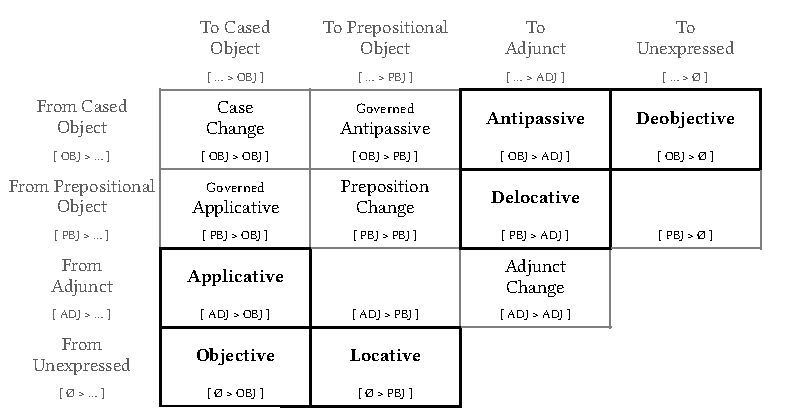
\includegraphics[width=\textwidth]{figures/objectdiatheses.pdf}
\caption{Names for isolated object remappings}\label{fig:objectdiatheses}}
\end{figure}

I\paragraphnumber{[2.123]} will discuss the different role-remappings
from Figure~\ref{fig:objectdiatheses} in four subsections. First, I will
summarise the various kinds of applicatives and antipassives (mid left
and mid top), then the objectives and deobjectives (top right and left
bottom), followed by locative and delocative diatheses (mid bottom and
mid right), and finally the symmetrical exchanges (on the diagonal).

\hypertarget{sec:intro-applicative-antipassive}{%
\subsubsection{Applicatives \&
antipassives}\label{sec:intro-applicative-antipassive}}

Applicatives\paragraphnumber{[2.124]} and antipassives are very similar,
though reversed. \textsc{applicatives (adj\,›\,obj)} change a
prepositional phrase into a case-marked phrase, while
\textsc{antipassives (obj\,›\,adj)} convert a case-marked phrase into a
prepositional phrase. Given this affinity, instead of antipassive it
might be better to call such remappings ``antiapplicative'' (e.g.
\citealt{haspelmath2004c}: 1132) or ``deapplicative'' (in line with the other names below).

By\paragraphnumber{[2.125]} removing or adding an object, applicatives
and antipassives change the transitivity of the sentence. However,
because case marking in German is nominative/accusative aligned, changes
in transitivity are not reflected in the marking of the subject. This is
crucially different from languages with ergatively aligned case marking,
in which antipassives also include a change in the marking of the
subject, namely from ergative to absolutive (and vice versa with
applicatives). Terminologically, these two situations might be
distinguished by using the term ``deapplicative'' for
nominative/accusative languages and reserve ``antipassive'' for
ergative/absolutive languages. I decided against that distinction and
the term ``antipassive'' will be used throughout in this book with this
explicit caveat.

Applicatives\paragraphnumber{[2.126]} occur frequently with the addition
of a preverb, like in the alternation between \emph{steigen auf} `to
climb' and \emph{besteigen} `to mount' (\ref{ex2.76}), see
Sec­tion~\ref{sec:preverb-applicative}.

\begin{samepage}
\ea \judgewidth{} \label{ex2.76} \textsc{applicative (adj\,›\,obj)}
  \ea [] { Sie steigt auf den Berg. }
  \ex [] { Sie besteigt den Berg. }
  \z
\z
\end{samepage}

Antipassives\paragraphnumber{[2.127]} in German are often unmarked (see
further below), but an example of an antipassive with a clear markedness
direction is the alternation between \emph{treffen} `to meet' and
reflexive \emph{sich treffen mit} 'to meet with (\ref{ex2.77}), see
Sec­tion~\ref{sec:reflexive-mit-antipassive}.

\begin{samepage}
\ea \judgewidth{} \label{ex2.77} \textsc{antipassive (obj\,›\,adj)}
  \ea [] { Ich treffe dich. }
  \ex [] { Ich treffe mich mit dir. }
  \z
\z
\end{samepage}

The\paragraphnumber{[2.128]} object of applicatives and antipassives is
typically an accusative, but datives can also be targeted. An example of
a dative applicative is the alternation between \emph{stammen aus} `to
hail from' and \emph{entstammen} `to be descended from' (\ref{ex2.78}),
see Sec­tion~\ref{sec:preverb-dative-applicative}. An example of a dative
antipassive is the covert alternation of \emph{berichten} `to report'
(\ref{ex2.79}), see
Sec­tion~\ref{sec:prepositions-dative-antipassive-accusative}.

\begin{samepage}
\ea \judgewidth{} \label{ex2.78} \textsc{dative applicative
(adj\,›\,obj)}
  \ea [] { Ich stamme aus einem Adelsgeschlecht. }
  \ex [] { Ich entstamme einem Adelsgeschlecht }
  \z
\z
\end{samepage}

\begin{samepage}
\ea \judgewidth{} \label{ex2.79} \textsc{dative antipassive
(obj\,›\,adj)}
  \ea [] { Er berichtet dem Vorstand alles. }
  \ex [] { Er berichtet alles an den Vorstand. }
  \z
\z
\end{samepage}

In\paragraphnumber{[2.129]} the discussion of diatheses in this book I
consistently distinguish \textsc{governed applicatives (pbj\,›\,obj)}
and \textsc{governed antipassives (obj\,›\,pbj)} when the prepositional
phrase is a governed preposition (see
Sec­tion~\ref{sec:prepositions-identifying-governed-prepositions}). An
example of a governed applicative is the diathesis between
\emph{arbeiten an} `to work on' (with a governed preposition \emph{an})
and \emph{bearbeiten} `to edit, adapt' (\ref{ex2.80}), see
Sec­tion~\ref{sec:preverb-governed-applicative}. An example of a governed
antipassive is the diathesis between \emph{beklagen} `to lament' and
\emph{sich beklagen} `to complain' (with a governed preposition
\emph{über}) (\ref{ex2.81}), see
Sec­tion~\ref{sec:reflexive-accusative-antipassive}. However, the
differentiation between the governed and non-governed
applicative/antipassive does not currently allow for any promising
semantic or structural generalisations, so this differentiation might
grammatically be unnecessary to explain German sentence structure.

\begin{samepage}
\ea \judgewidth{} \label{ex2.80} \textsc{governed applicative
(pbj\,›\,obj)}
  \ea [] { Ich arbeite an dem Text.\\
(Ich arbeite daran, dass der Text fertig wird.) }
  \ex [] { Ich bearbeite den Text. }
  \z
\z
\end{samepage}

\begin{samepage}
\ea \judgewidth{} \label{ex2.81} \textsc{governed antipassives
(obj\,›\,pbj)}
  \ea [] { Ich beklage den Lärm. }
  \ex [] { Ich beklage mich über den Lärm.\\
(Ich beklage mich darüber, dass es so laut ist.) }
  \z
\z
\end{samepage}

There\paragraphnumber{[2.130]} are a many diatheses with a
role-remapping between adjunct and object that do not have any overt
indication of a direction. Without explicit marking it is difficult to
decide whether such diatheses are cases of (applicative) promotion
\textsc{(adj\,›\,obj)} or (antipassive) demotion \textsc{(obj\,›\,adj)}.
For the sake of organisation in this book I classify such covert
alternations on the basis of (debatable) semantic intuitions and
parallels to other overtly marked diatheses.

Most\paragraphnumber{[2.131]} covert diatheses with an alternation
between prepositional phrases and case-marked arguments are classified
here as \textsc{antipassive}, like in the alternation between
\emph{schießen auf} `to aim at' and \emph{schießen} `to shoot'
(\ref{ex2.82}), see
Sec­tion~\ref{sec:prepositions-accusative-antipassive}. This is also
widespread with datives (\ref{ex2.83}), see
Sec­tion~\ref{sec:prepositions-dative-antipassive-accusative}. In such
examples, I judge the case-marking to be more basic than the
prepositional phrase.

\begin{samepage}
\ea \judgewidth{} \label{ex2.82} \textsc{covert antipassive
(obj\,›\,adj)}
  \ea [] { Ich schieße den Bären. }
  \ex [] { Ich schieße auf den Bären. }
  \z
\z
\end{samepage}

\begin{samepage}
\ea \judgewidth{} \label{ex2.83} \textsc{covert dative antipassive
(obj\,›\,adj)}
  \ea [] { Ich schreibe dir einen Brief.\\
 }
  \ex [] { Ich schreibe einen Brief an dich. }
  \z
\z
\end{samepage}

In\paragraphnumber{[2.132]} contrast, there is a widespread alternation
between datives and beneficiary \emph{für} prepositional phrases
(\ref{ex2.84}) that I classify as an \textsc{applicative}, see
Sec­tion~\ref{sec:prepositions-benefactive-dative}. In this example the
beneficiary dative seems to be the derived construction.

\begin{samepage}
\ea \judgewidth{} \label{ex2.84} \textsc{covert applicative: beneficiary
raising (adj\,›\,obj)}
  \ea [] { Er kocht eine Suppe für mich. }
  \ex [] { Er kocht mir eine Suppe. }
  \z
\z
\end{samepage}

\hypertarget{par:possraising}{
\paragraphnumber{[2.133]}\label{par:possraising}}There is a further kind
of covert diathesis with a dative object, conventionally called
\textsc{possessor raising}. In such diatheses there is an alternation
between a possessor (typically expressed as an adnominal genitive) and a
dative (\ref{ex2.85}). The dative can alternate with the possessor of a
nominative subject (see
Sec­tion~\ref{sec:case-possessor-of-nominative-to-dative-experiencer}),
an accusative object (see
Sec­tion~\ref{sec:case-possessor-accusative-to-dative}) or an obligatory
location (see
Sec­tion~\ref{sec:prepositions-possessor-of-location-to-dative-experiencer}).
Following widespread convention, I classify these diatheses as promotion
\textsc{(adj\,›\,obj)}

\begin{samepage}
\ea \judgewidth{} \label{ex2.85} \textsc{covert applicative: possessor
raising (adj\,›\,obj)}
  \ea [] { Er schneidet meine Haare. }
  \ex [] { Er schneidet mir die Haare. }
  \z
\z
\end{samepage}

These\paragraphnumber{[2.134]} two covert kinds of dative applicative
(viz.~beneficiary and possessor applicative) are semantically and
structurally clearly distinct. The datives that show a possessive
alternation (\ref{ex2.85}) are semantically experiencers. In contrast,
datives that alternate with \emph{für} prepositional phrases
(\ref{ex2.84}) are semantically beneficiaries. In especially crafted
context it might be possible to evoke either reading for the same
sentence (\ref{ex8.90}).

\begin{samepage}
\ea \judgewidth{?} \label{ex2.86} 
  \ea [\textsuperscript{?}] { Ich schneide dir (zuliebe) in den (meinen)
Finger.\\
(= Ich schneide für dich in meinen Finger.) }
  \ex [] { Ich schneide dir in den (deinen) Finger.\\
(= Ich schneide in deinen Finger.) }
  \z
\z
\end{samepage}

\hypertarget{sec:intro-objective-deobjective}{%
\subsubsection{Objectives \&
deobjectives}\label{sec:intro-objective-deobjective}}

A\paragraphnumber{[2.135]} \textsc{deobjective diathesis (obj\,›\,ø)} is
a diathesis that drops an object, i.e.~a role cannot be expressed
anymore (the term is taken from \citealt{haspelmath2004c}: 1131). 
A deobjective drop is illustrated in (\ref{ex2.87}) with
an alternation from \emph{kaufen} `to buy' to \emph{einkaufen} `to
shop', see Sec­tion~\ref{sec:preverb-accusative-drop} for an extensive
discussion.

\begin{samepage}
\ea \judgewidth{} \label{ex2.87} \textsc{deobjective (obj\,›\,ø)}
  \ea [] { Ich habe gestern ein Buch gekauft. }
  \ex [] { Ich habe gestern eingekauft. }
  \z
\z
\end{samepage}

A\paragraphnumber{[2.136]} special variant of a deobjective occurs with
verbs that apply to the body, like \emph{verbrennen} `to burn'
(\ref{ex2.88}). In such constructions, a reflexive pronoun is necessary.
This diathesis is called \textsc{endoreflexive}
(\citealt{haspelmath1987}: 27--28), see
Sec­tion~\ref{sec:reflexive-accusative-drop} for an extensive discussion.

\begin{samepage}
\ea \judgewidth{} \label{ex2.88} \textsc{deobjective (endoreflexive)
(obj\,›\,ø)}
  \ea [] { Er verbrennt das Buch. }
  \ex [] { Er verbrennt sich. }
  \z
\z
\end{samepage}

\hypertarget{par:objective}{
\paragraphnumber{[2.137]}\label{par:objective}}An \textsc{objective
diathesis (ø\,›\,obj)} is a diathesis that adds a new object, i.e.~a
completely new role is introduced in the form of an object. An example
of an overtly marked object addition is the alternation from
\emph{zaubern} `to perform magic' to \emph{verzaubern} `to enchant'
(\ref{ex2.89}). In this example the new object is simply an
\textsc{added patient} to an erstwhile intransitive action. Such object
additions are frequently attested with preverbs like \emph{ver-}, see
Sec­tion~\ref{sec:preverb-accusative-addition}.

\begin{samepage}
\ea \judgewidth{} \label{ex2.89} \textsc{objective: added patient
(ø\,›\,obj)}
  \ea [] { Sie zaubert. }
  \ex [] { Sie verzaubert mich. }
  \z
\z
\end{samepage}

A\paragraphnumber{[2.138]} semantically special kind of diathesis
introduces a new \textsc{added result} object. Such an objective
diathesis adds an object that is the result of performing the activity
described by the predicate. An overtly marked example is presented in
(\ref{ex2.90}) with the diathesis between \emph{arbeiten} `to work' and
the inherent reflexive \emph{sich etwas erarbeiten} `to acquire
something through work', see
Sec­tion~\ref{sec:preverb-reflexive-resultative}. The result of the work
is added as an object in (\ref{ex2.90}b).\footnote{Here I consciously
  avoid the term ``resultative'' for this phenomenon to avoid confusion.
  First, I already use the term ``resultative'' in this book for a
  special class of preverbial adjectives (see
  Sec­tion~\ref{sec:adverbial-resultative-predicates}). Second, the term
  ``resultative'' is also frequently used in the literature for an
  aspectual concept, namely to indicate a special kind of state induced
  as the result of performing the predicate (e.g.
  \citealt{nedjalkov1988a}).}

\begin{samepage}
\ea \judgewidth{} \label{ex2.90} \textsc{objective: added result
(ø\,›\,obj)}
  \ea [] { Ich arbeite. }
  \ex [] { Ich erarbeite mir ein Vermögen.\\
(= Ich arbeite, und das Resultat davon ist, dass ich ich ein Vermögen
besitze.) }
  \z
\z
\end{samepage}

Objectives\paragraphnumber{[2.139]} and deobjectives are frequently
attested without any overt marking (cf.~ambitransitive/labile verbs),
and in such ``covert'' diatheses it is difficult to establish a
direction. As already noted above, for the sake of organisation in this
book I classify such covert alternations on the basis of (often
debatable) semantic intuitions and parallels with other overtly marked
diatheses. For example, the verb \emph{stören} `to disturb'
(\ref{ex2.91}) can be used both with and without an accusative object,
see Sec­tion~\ref{sec:case-accusative-drop}. This is classified here as a
deobjective diathesis. Such unmarked object drops are also attested with
datives, see Sec­tion~\ref{sec:case-dative-drop}, and with governed
prepositions, see Sec­tion~\ref{sec:prepositions-demotion-of-object}. The
dropping of an object is also often used to put the focus on the action
itself, but then it is typically attested with an adverbial, see
Sec­tion~\ref{sec:adverbial-action-focus} for an extensive discussion.

\begin{samepage}
\ea \judgewidth{} \label{ex2.91} \textsc{covert deobjective (obj\,›\,ø)}
  \ea [] { Du störst die Veranstaltung. }
  \ex [] { Du störst. }
  \z
\z
\end{samepage}

In\paragraphnumber{[2.140]} contrast, the verb \emph{stottern} `to
stutter' is classified here as an example of a covert object addition
(\ref{ex2.92}), although there is no formal differentiation from the
previous example of a covert object drop (\ref{ex2.91}). The intuition
is that \emph{stottern} is basically intransitive (and any accusative
object is thus added), while \emph{stören} is basically transitive (and
any missing object is thus dropped). Correlated with this proposed
difference is the fact that covert object addition with \emph{stottern}
has an \textsc{added result} interpretation (\ref{ex2.92}b). However, it
remains to be seen whether there is really a substantive difference
between these two kinds of verbs (see
Sec­tion~\ref{sec:case-accusative-addition} for an extensive discussion).

\begin{samepage}
\ea \judgewidth{} \label{ex2.92} \textsc{covert objective: added result
(ø\,›\,obj)}
  \ea [] { Er stotterte. }
  \ex [] { Er stotterte eine Entschuldigung.\\
(= Er stotterte, und das Resultat davon ist eine Entschuldigung.) }
  \z
\z
\end{samepage}

\hypertarget{sec:intro-locative-delocative}{%
\subsubsection{Locatives \&
delocatives}\label{sec:intro-locative-delocative}}

A\paragraphnumber{[2.141]} \textsc{locative diathesis (ø\,›\,pbj)} is a
diatheses that adds an obligatory location phrase to the clause. For
example, the transitive \emph{befehlen} `to order' marks the ordered
person as an accusative (\ref{ex2.93}a). With a (directional) locative
phrase \emph{an die Front} `to the frontline' the sentence obtains a
caused-motion reading (\ref{ex2.93}b), see
Sec­tion~\ref{sec:prepositions-transitive-location-as-result}. Note that
there is no profound association between such a \emph{locative
diathesis} and the widespread phenomenon of a \emph{locative case}. Both
terms simply use the term ``locative'' to describe the fact that the
marking of location is concerned.

\begin{samepage}
\ea \judgewidth{} \label{ex2.93} \textsc{locative: caused motion
(ø\,›\,pbj)}
  \ea [] { Ich befehle eine Armee. }
  \ex [] { Ich befehle die Armee an die Front.\\
(= Ich befehle, und dadurch geht die Armee an die Front.) }
  \z
\z
\end{samepage}

Even\paragraphnumber{[2.142]} more noteworthy, such a caused-motion
diathesis is also possible with many intransitive verbs like
\emph{schwitzen} `to sweat' (\ref{ex2.94}a). With such verbs, a locative
diathesis not only adds a location, like \emph{in mein Hemd} `in my
shirt', but also an added-result accusative object, like \emph{einen
Fleck} `a stain' (\ref{ex2.94}b), see
Sec­tion~\ref{sec:prepositions-intransitive-location-as-result}.

\begin{samepage}
\ea \judgewidth{} \label{ex2.94} \textsc{locative: caused motion \&
added result (ø\,›\,pbj\,+\,ø\,›\,obj)}
  \ea [] { Ich schwitze. }
  \ex [] { Ich schwitze einen Fleck in mein Hemd.\\
(= Ich schwitze, und dadurch ist ein Fleck in meinem Hemd entstanden.) }
  \z
\z
\end{samepage}

\hypertarget{par:delocative}{
\paragraphnumber{[2.143]}\label{par:delocative}}The reversal of a
locative diathesis is a \textsc{delocative diathesis (pbj\,›\,adj)}. In
such a diathesis an obligatory location loses its obligatory status and
is often completely dropped. An example of such a diathesis is shown in
(\ref{ex2.95}) with the alternation between \emph{stecken} `to put into'
and \emph{verstecken} `to hide'. The verb \emph{stecken} needs an
obligatory location (\ref{ex2.95}a,b). Such an obligatory location is
classified here as a \textsc{pbj} prepositional object (see
Sec­tion~\ref{sec:intro-arguments-utterance-valency}). The situation is
different with the verb \emph{verstecken}. With this verb the location
is an \textsc{adj} optional adjunct and can be left out (see
Sec­tion~\ref{sec:preverb-transitive-antiresultative} for an extensive
discussion).

\begin{samepage}
\ea \judgewidth{*} \label{ex2.95} \textsc{delocative (pbj\,›\,adj)}
  \ea [] { Ich stecke das Geschenk in den Schrank. }
  \ex [*] { Ich stecke das Geschenk. }
  \ex [] { Ich verstecke das Geschenk in dem Schrank. }
  \ex [] { Ich verstecke das Geschenk. }
  \z
\z
\end{samepage}

\hypertarget{sec:intro-symmetrical-object}{%
\subsubsection{Symmetrical object
diatheses}\label{sec:intro-symmetrical-object}}

Symmetrical\paragraphnumber{[2.144]} object diatheses are rare in
German. A \textsc{case change (obj\,›\,obj)} is illustrated in
(\ref{ex2.96}) by the alternation between \emph{folgen} `to follow'
(with dative) and \emph{verfolgen} `to chase' (with accusative), see
Sec­tion~\ref{sec:preverb-dative-accusative}.

\begin{samepage}
\ea \judgewidth{} \label{ex2.96} \textsc{case change (obj\,›\,obj)}
  \ea [] { Ich folge dem Auto. }
  \ex [] { Ich verfolge das Auto. }
  \z
\z
\end{samepage}

A\paragraphnumber{[2.145]} \textsc{governed preposition change
(pbj\,›\,pbj)} does occur in German, but such diatheses have not been
explicitly collected in this book. Possible examples are \emph{arbeiten
an} `to work on' (\ref{ex2.97}a) changing into \emph{sich durcharbeiten}
`to work through' (\ref{ex2.97}b) or \emph{sorgen für} `take care of'
(\ref{ex2.97}c) changing into \emph{sich sorgen um} `to worry about'
(\ref{ex2.97}d).

\begin{samepage}
\ea \judgewidth{} \label{ex2.97} \textsc{governed preposition change
(pbj\,›\,pbj)}
  \ea [] { Er arbeitet an den Daten. }
  \ex [] { Er arbeitet sich durch die Daten. }
  \ex [] { Er sorgt für seine Mutter. }
  \ex [] { Er sorgt sich um seine Mutter. }
  \z
\z
\end{samepage}

An\paragraphnumber{[2.146]} \textsc{adjunct change (adj\,›\,adj)} is,
according to my definitions, not a diathesis at all, as adjuncts are not
lexically specific. However, the change between a possessor \emph{dein}
`your' (\ref{ex2.98}a) and a non-governed prepositional phrase \emph{von
dir} `from you' (\ref{ex2.98}b) can be seen as as a borderline examples,
see Sec­tion~\ref{sec:prepositions-possessor-to-preposition}.

\begin{samepage}
\ea \judgewidth{} \label{ex2.98} \textsc{adjunct change (adj\,›\,adj)}
  \ea [] { Ich erwarte dein Geschenk. }
  \ex [] { Ich erwarte ein Geschenk von dir. }
  \z
\z
\end{samepage}

\hypertarget{sec:intro-object-chains}{%
\subsection{Chained object diatheses}\label{sec:intro-object-chains}}

Chains\paragraphnumber{[2.147]} of object diatheses (i.e.~chains with
the object in the middle of the chain) can always be interpreted as a
combination of two isolated object diatheses from the previous section.
However, not all theoretically possible combinations are attested (see
Figure~\ref{fig:objectchains}). The most frequently attested chained
object diatheses are the highlighted variants of \textsc{object
exchange} (see
Sec­tions~\ref{sec:intro-object-exchange}, \ref{sec:intro-chained-other-object}).
A few incidental examples of \textsc{chained case change} are also
attested (see Sec­tion~\ref{sec:intro-chained-case-change}).

\begin{figure}
\hypertarget{fig:objectchains}{%
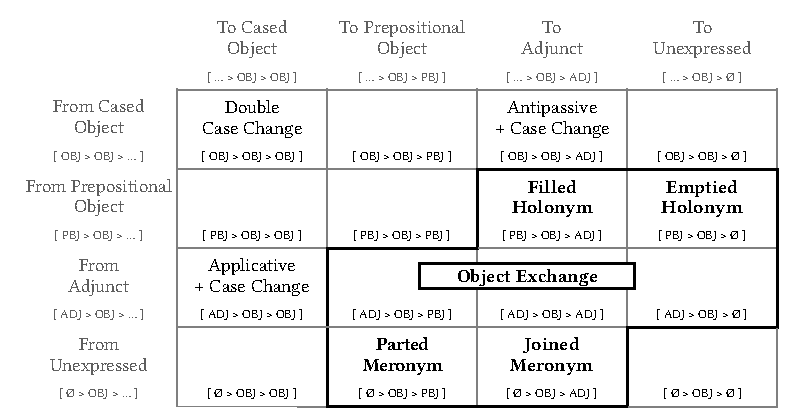
\includegraphics[width=\textwidth]{figures/objectchains2.pdf}
\caption{Names for chains of object diathesis}\label{fig:objectchains}}
\end{figure}

\hypertarget{sec:intro-object-exchange}{%
\subsubsection{Object exchange}\label{sec:intro-object-exchange}}

The\paragraphnumber{[2.148]} highlighted diatheses in
Figure~\ref{fig:objectchains} are collectively called \textsc{object
exchange} because as part of the role-remapping the accusative marking
is exchanged from one role to another. These diatheses are used with
verbs that involve some kind of part/whole relation between the two
roles involved. A typical example (\ref{ex2.99}) is the diathesis
between \emph{schmieren} `to smear' and \emph{beschmieren} `to spread'
(discussed in detail in
Sec­tion~\ref{sec:preverb-applicative-antipassive}). In this example an
\emph{auf} prepositional phrase turns into a new accusative, while the
old accusative is turned into a \emph{mit} prepositional phrase. So,
syntactically the role marked as an accusative object is exchanged from
\emph{Salbe} `ointment' to \emph{Wunde} `wound'. Semantically, the
\emph{Wunde} is the ``whole'' to which the \emph{Salbe} is applied.

\begin{samepage}
\ea \judgewidth{} \label{ex2.99} \textsc{object exchange}
  \ea [] { Ich schmiere die Salbe auf die Wunde. }
  \ex [] { Ich beschmiere die Wunde mit der Salbe. }
  \z
\z
\end{samepage}

Different\paragraphnumber{[2.149]} variants of such object exchange show
an astonishingly strong correlation between syntactic structure and
semantic interpretation. Basically, promotions have the effect that the
new object role is a part of the old object role (i.e.~the new object is
a \textsc{meronym}), while demotions have the reverse effect in that the
new object role encompasses the old object role (i.e.~the new object is
a \textsc{holonym}). To appreciate this generalisation it is important
to recall how demotions and promotions are defined for chained
diatheses. This definition is not trivial because chained diatheses are
always a combination of both a promotion and a demotion. So the question
is which of the two ``wins''.

By\paragraphnumber{[2.150]} definition (cf.
Sec­tion~\ref{sec:intro-remapping}), a chained diathesis is deemed to be
an overall demotion when the demotion-part is stronger than the
promotion-part, and vice versa. The strength is measured as the size of
the ``jump'' on the \textsc{macrorole hierarchy}, repeated here in
(\ref{ex2.100}). Additionally, the overall chain exhibits varying
intensity: the larger the difference in jump size between demotion-part
and promotion-part, the more extreme the overall chain.

\begin{samepage}
\ea \judgewidth{} \label{ex2.100} \textsc{macrorole hierarchy}\\
  \textsc{sbj » obj » pbj » adj » ø}
\z
\end{samepage}

Concretely,\paragraphnumber{[2.151]} the promotion of an object exchange
can be either an objective \textsc{(ø\,›\,obj)} (``three steps up''), an
applicative \textsc{(adj\,›\,obj)} (``two steps up'') or an
oblig­a­tory-loc­ation applicative \textsc{(pbj\,›\,obj)} (``one step
up''). In reverse, the demotion can be either a deobjective
\textsc{(obj\,›\,ø)} (``three steps down''), an antipassive
\textsc{(obj\,›\,adj)} (``two steps down'') or an oblig­a­tory-loc­ation
antipassive \textsc{(obj\,›\,pbj)} (``one step down''). Combining two of
these leads to an overall assessment of the chained diathesis. This
whole concept of chained demotions/promotions can be visualised by
considering the top-right to bottom-left diagonal in
Figure~\ref{fig:objectchains}. The top-right corner
\textsc{(obj\,›\,obj\,›\,ø)} is the most extreme demotion (``net four
down'') and the bottom-left corner \textsc{(ø\,›\,obj\,›\,obj)} is the
most extreme promotion (``net four up''). All other possibilities are
situated somewhere in between these extremes on this diagonal.

For\paragraphnumber{[2.152]} example, consider again the diathesis from
\emph{schmieren} to \emph{beschmieren}, repeated below in
(\ref{ex2.101}). It consist of a promotion from a prepositional phrase
\emph{auf die Wunde} to an accusative \emph{die Wunde} and a demotion
from an accusative \emph{die Salbe} to a prepositional phrase \emph{mit
der Salbe}. The promotion starts from an obligatory location
(\ref{ex2.101}a,b), i.e.~this is an oblig­a­tory-loc­ational applicative
\textsc{(pbj\,›\,obj)}. In contrast, the demotion ends in an optional
instrumental phrase (\ref{ex2.101}c,d), i.e.~this is an antipassive
diathesis \textsc{(obj\,›\,adj)}. Now, the antipassive demotion (``two
steps down'') is a bigger jump on the macrorole hierarchy than the
oblig­a­tory-loc­ation promotion (``one step up''), so the whole object
exchange \textsc{(pbj\,›\,obj\,›\,adj)} is classified as a demotion, be
it a minor one (``net one step down'').\largerpage

\begin{samepage}
\ea \judgewidth{*} \label{ex2.101} \textsc{demoted object exchange
(pbj\,›\,obj\,›\,adj)}
  \ea [] { Ich schmiere die Salbe auf die Wunde. }
  \ex [*] { Ich schmiere die Salbe. }
  \ex [] { Ich beschmiere die Wunde mit Salbe. }
  \ex [] { Ich beschmiere die Wunde. }
  \z
\z
\end{samepage}

According\paragraphnumber{[2.153]} to the above mentioned
generalisation, such an overall demotion coincides with the fact that
the new object \emph{Wunde} `wound' is a holonym to which the old
meronymic object \emph{Salbe} `ointment' is applied. To be precise, the
terms \textsc{meronym} and \textsc{holonym} are language-specific
classifications as observed in the structure of German. So, not all
examples necessarily correspond to any (universal) semantic
conceptualisation of the terms holonym/meronym. For example, German
verbs that describe an act of covering (e.g.~\emph{schmieren} `to
smear') or wrapping (e.g.~\emph{wickeln} `to wrap around') consistently
treat the cover/wrap alike to other meronyms and the covered/wrapped
object alike to other holonyms. That is no statement about what it
semantically means to be a meronym or holonym. It is just a statement
about the distribution of syntactic structures among German verbs as
they take part in object exchange.

\hypertarget{sec:intro-demoted-object-exchange}{%
\subsubsection{Demoted object
exchange}\label{sec:intro-demoted-object-exchange}}

There\paragraphnumber{[2.154]} are two different kinds of object
exchange with demotion, namely the \textsc{filled holonym} and the
\textsc{emptied holonym} object exchange. These two kinds of exchange
correlate with the intensity of the demotion. A minor demotion manifests
a fil­led-holo­nym object exchange, while a more extreme form of demotion
expresses an emptied-holonym object exchange.\largerpage

Typically,\paragraphnumber{[2.155]} a \textsc{filled holonym} diathesis
is expressed by a minor demotion (``net one step down''), as illustrated
with \emph{schmieren/beschmieren} above in (\ref{ex2.101}). Note that in
that example, the holonym \emph{Wunde} is not literally `filled with'
the meronym \emph{Salbe}. However, with many other examples, like
\emph{pflanzen/bepflanzen} `to plant' below (\ref{ex2.102}), the holonym
\emph{Garten} `garden' is literally filled with the meronym
\emph{Tulpen} `tulips'. In accordance with this being a minor overall
demotion (``net one step down''), the new accusative object after the
object exchange is a filled holonym.

Note\paragraphnumber{[2.156]} that with \emph{pflanzen/bepflanzen}
(\ref{ex2.102}) the pre-diathesis location phrase \emph{in den Garten}
is not obligatory (\ref{ex2.102}a,b), so the resulting diathesis is
symmetric \textsc{(adj\,›\,obj\,›\,adj)}. This is the kind of minor
syntactic variation that is indicated in Figure~\ref{fig:objectchains}
with the unnamed boxes in the centre of the highlighted object-exchange
domain. Still, this diathesis is clearly an example of a fil­led-holo­nym
object exchange because the change in prepositions from \emph{in} (with
unmarked \emph{pflanzen}) to \emph{mit} (with marked \emph{bepflanzen})
fits in perfectly with other fil­led-holo­nym examples (cf.
Sec­tion~\ref{sec:preverb-applicative-antipassive}).

\ea\label{ex2.102}\textsc{symmetric object exchange: filled holonym (adj\,›\,obj\,›\,adj)}
  \ea Ich pflanze Tulpen in den Garten.
  \ex Ich pflanze Tulpen.
  \ex Ich bepflanze den Garten mit Tulpen. 
  \ex Ich bepflanze den Garten. 
  \z
\z

The\paragraphnumber{[2.157]} second kind of demoted object exchange is
the \textsc{emptied holonym} diathesis, expressed with a more extreme
demotion (``net two steps down''). This is illustrated in
(\ref{ex2.103}) with the diathesis between the verb \emph{klopfen} `to
pound' and \emph{ausklopfen} `to beat out' (cf.
Sec­tion~\ref{sec:preverb-location-antiresultative}). The unmarked verb
\emph{klopfen} (\ref{ex2.103}a) takes an accusative object role that
expresses the result of the pounding (\emph{Staub} `dust'). The pounded
object role (\emph{Mantel} `coat') is expressed as an obligatory
location phrase (\ref{ex2.103}b). Crucially, the accusative object role
in this construction is a component part (meronym) of the locational
object role (holonym). The diathesis from \emph{klopfen} to
\emph{ausklopfen} (\ref{ex2.103}c) completely drops the meronym
\emph{Staub} from the sentence \textsc{(obj\,›\,ø)} and promotes the
holonym \emph{Mantel} to accusative \textsc{(pbj\,›\,obj)}. The
meronymic role \emph{Staub} cannot be expressed anymore at all after the
diathesis (\ref{ex2.103}d). In accordance with this large overall
demotion (``net two steps down''), the new holonymic accusative object
\emph{Mantel} is semantically ``emptied'' from its old meronymic
accusative object \emph{Staub} by the action \emph{klopfen}. So the new
accusative object after this object exchange is an emptied holonym.

\begin{samepage}
\ea \judgewidth{*} \label{ex2.103} \textsc{demoted object exchange:
emptied holonym (pbj\,›\,obj\,›\,ø)}
  \ea [] { Ich klopfe den Staub von meinem Mantel. }
  \ex [*] { Ich klopfe den Staub. }
  \ex [] { Ich klopfe meinen Mantel aus. }
  \ex [*] { Ich klopfe meinen Mantel von den Staub aus. }
  \z
\z
\end{samepage}

\hypertarget{sec:intro-promoted-object-exchange}{%
\subsubsection{Promoted object
exchange}\label{sec:intro-promoted-object-exchange}}

There\paragraphnumber{[2.158]} are also two different kinds of object
exchange with promotion, namely the \textsc{joined meronym} and the
\textsc{parted meronym} object exchange. These two kinds of object
exchange correlate with the intensity of the promotion. A minor
promotion manifests a joined-meronym object exchange, while a more
extreme form of promotion expresses a parted-meronym object exchange.
Basically, these diatheses are reversals of the two demoted object
exchanges discussed in the previous section.

The\paragraphnumber{[2.159]} \textsc{joined meronym} object exchange
occurs with less extreme promotions (``net one step up''). This is
illustrated here with the diathesis from \emph{nähen} `to sew' to
\emph{festnähen} `to fixate by sewing' (\ref{ex2.104}). The original
object role \emph{Bluse} `blouse' (\ref{ex2.104}a) turns into an
optional \emph{an} prepositional phrase (\ref{ex2.104}b,c). This part of
the chain is an antipassive diathesis \textsc{(obj\,›\,adj)}, i.e.~``two
steps down''. At the same time a new object role \emph{Knopf} `button'
is introduced. This role cannot be expressed in the construction before
the diathesis (\ref{ex2.104}a). So, this part of the chain is an
objective diathesis \textsc{(ø\,›\,obj)}, i.e.~``three steps up''. The
promotion is larger than the demotion, so the whole diathesis overall is
a promotion, although a minor one, i.e.~``net one step up''. As
predicted for promotions, the new object \emph{Knopf} semantically is a
meronymic part of the original object \emph{Bluse}. Further, in
accordance with the promotion being minor, the verb \emph{nähen}
describes a situation in which the new object \emph{Knopf} is physically
connected to the holonymic \emph{Bluse}. In summary, the new object is a
joined meronym.

\begin{samepage}
\ea \judgewidth{} \label{ex2.104} \textsc{promoted object exchange:
joined meronym (ø\,›\,obj\,›\,adj)}
  \ea [] { Ich habe eine Bluse genäht. }
  \ex [] { Ich habe den Knopf an die Bluse festgenäht. }
  \ex [] { Ich habe den Knopf festgenäht. }
  \z
\z
\end{samepage}

In\paragraphnumber{[2.160]} some examples the joined-meronym object
exchange allows for optional prepositional phrases at both sides of the
diathesis, resulting in a symmetric diathesis
\textsc{(adj\,›\,obj\,›\,adj)}. For example, this is attested with the
diathesis from \emph{massieren} `to massage' (\ref{ex2.105}a,b) to
\emph{einmassieren} `to massage in' (\ref{ex2.105}c,d). Still, this
diathesis is clearly an example of a joined-meronym object exchange
because the change in preposition from \emph{mit} (with unmarked
\emph{massieren}) to \emph{in} (with marked \emph{einmassieren}) is
completely parallel to all other joined-meronym examples (cf.
Sec­tion~\ref{sec:preverb-applicative-in-antipassive}). Semantically, the
new accusative object role (\emph{Balsam}, `balm') is a meronym of the
old object role (\emph{Muskeln} `muscles'), and this new object role is
applied to the old object role to become a part of it by the verb
\emph{massieren}. So, even though the diathesis is symmetric, the new
object is syntactically and semantically a joined meronym.

\begin{samepage}
\ea \judgewidth{} \label{ex2.105} \textsc{symmetric object exchange:
joined meronym (adj\,›\,obj\,›\,adj)}
  \ea [] { Ich habe die Muskeln mit Balsam massiert. }
  \ex [] { Ich habe die Muskeln massiert. }
  \ex [] { Ich habe den Balsam in die Muskeln einmassiert. }
  \ex [] { Ich habe den Balsam einmassiert. }
  \z
\z
\end{samepage}

The\paragraphnumber{[2.161]} \textsc{parted meronym} object exchange
occurs with more extreme promotions (``net two steps up''). For example,
the verb \emph{waschen} `to wash' normally takes an accusative object
role that is the washee, here \emph{Hose} `trousers' (\ref{ex2.106}a).
There is a covert diathesis that introduces a new object role that
cannot be expressed earlier, here \emph{Fleck} `stain' (\ref{ex2.106}b).
this addition is an objective promotion \textsc{(ø\,›\,obj)},
i.e.~``three steps up''. At the same time, the original accusative is
turned into a locational prepositional phrase and this location phrase
cannot be left out (\ref{ex2.106}c). This is an oblig­a­tory-loc­ation
antipassive \textsc{(obj\,›\,pbj)}, i.e ``one step down''. This
diathesis is thus an extreme promotion overall, i.e.~``net two steps
up''. Accordingly, the new meronymic object \emph{Fleck} is semantically
a component part of the original holonymic object \emph{Hose} and it is
removed from it by the action \emph{waschen}. In summary, the new object
is a parted meronym.

\begin{samepage}
\ea \judgewidth{*} \label{ex2.106} \textsc{promoted object exchange:
parted meronym (ø\,›\,obj\,›\,pbj)}
  \ea [] { Ich wasche meine Hose. }
  \ex [] { Ich wasche den Fleck aus meiner Hose. }
  \ex [*] { Ich wasche den Fleck. }
  \z
\z
\end{samepage}

\hypertarget{sec:intro-chained-other-object}{%
\subsubsection{Other kinds of object
exchange}\label{sec:intro-chained-other-object}}

There\paragraphnumber{[2.162]} are a few other examples of object
exchange that do not fit in with the general pattern described above,
for example with \emph{zwingen/erzwingen} `to force' (\ref{ex2.107}a,b).
This chained diathesis is a remapping of the form
\textsc{(pbj\,›\,obj\,›\,adj)} because the preposition \emph{zu} is a
governed preposition (\ref{ex2.107}c). This diathesis is attested with
various verbs of persuasion (cf.
Sec­tion~\ref{sec:preverb-applicative-von-antipassive}). The demotion is
more prominent than the promotion, so this chain is overall a demotion.
Consequently, because it is the person being persuaded that is demoted I
call this a \textsc{persuadee demotion object exchange}.

\begin{samepage}
\ea \judgewidth{} \label{ex2.107} \textsc{object exchange: persuadee
demotion (pbj\,›\,obj\,›\,adj)}
  \ea [] { Er zwingt ihn zu einem Geständnis. }
  \ex [] { Er zwingt ihn dazu, ein Geständnis abzulegen. }
  \ex [] { Er erzwingt ein Geständnis (von ihm). }
  \z
\z
\end{samepage}

Another\paragraphnumber{[2.163]} example of an object exchange is
illustrated here with the verb \emph{bewundern} `to admire'
(\ref{ex2.108}), see
Sec­tion~\ref{sec:prepositions-possessor-to-preposition}. This verb (and
others like it) show a combination of a possessor-raising applicative
promotion \textsc{(adj\,›\,obj)} and a governed antipassive demotion
\textsc{(obj\,›\,pbj)} leading to the object exchange
\textsc{(adj\,›\,obj\,›\,pbj)}. The promotion is more prominent than the
demotion, so this chain is overall a promotion. I propose to call this a
\textsc{possessor raising object exchange}.

\begin{samepage}
\ea \judgewidth{} \label{ex2.108} \textsc{object exchange: possessor
raising (adj\,›\,obj\,›\,pbj)}
  \ea [] { Ich bewundere seine Ehrlichkeit. }
  \ex [] { Ich bewundere ihn für seine Ehrlichkeit. }
  \ex [] { Ich bewundere ihn dafür, dass er ehrlich ist. }
  \z
\z
\end{samepage}

\hypertarget{sec:intro-chained-case-change}{%
\subsubsection{Chained case
changes}\label{sec:intro-chained-case-change}}

Finally,\paragraphnumber{[2.164]} there are a few object chains
involving a change of case, shown at the top and the left of
Figure~\ref{fig:objectchains}. Note that a case change of
dative/genitive to accusative can be interpreted as a promotion, and the
reverse as a demotion, cf.
paragraph \hyperlink{par:corecase}{2.43} on page~\pageref{par:corecase},
but that perspective will not be expanded upon here.

Example\paragraphnumber{[2.165]} (\ref{ex2.109}) shows a combination of
a dative-to-accusative case change with an antipassive, resulting in a
chain \textsc{(obj\,›\,obj\,›\,adj)}. The verb \emph{schenken} `to gift'
takes a recipient in the dative and a patient in the accusative, while
the derived \emph{beschenken} `to gift' turns the accusative into a
prepositional phrase (i.e.~antipassive) and changes the dative
\emph{dir} into an accusative \emph{dich} (see
Sec­tion~\ref{sec:preverb-antipassive-dative-accusative}).

\begin{samepage}
\ea \judgewidth{} \label{ex2.109} \textsc{antipassive+case change
(obj\,›\,obj\,›\,adj)}
  \ea [] { Ich schenke dir ein Buch. }
  \ex [] { Ich beschenke dich mit einem Buch. }
  \z
\z
\end{samepage}

The\paragraphnumber{[2.166]} reverse situation, i.e.~a chain
\textsc{(adj\,›\,obj\,›\,obj)}, is attested with the diathesis between
\emph{drängen} `to urge' and the derived \emph{aufdrängen} `to impose'
(\ref{ex2.110}), see
Sec­tion~\ref{sec:preverb-applicative-accusative-to-dative}. In this
example a prepositional phrase changes into an accusative
(i.e.~applicative), while the accusative \emph{dich} changes to dative
\emph{dir}.

\begin{samepage}
\ea \judgewidth{} \label{ex2.110} \textsc{applicative+case change
(adj\,›\,obj\,›\,obj)}
  \ea [] { Ich dränge dich zu einem Abo. }
  \ex [] { Ich dränge dir ein Abo auf. }
  \z
\z
\end{samepage}

Finally,\paragraphnumber{[2.167]} an idiosyncratic diathesis is attested
with the verb \emph{rauben} `to rob' (\ref{ex2.111}), see
Sec­tion~\ref{sec:preverb-dative-accusative-genitive}. When this verb is
changed to \emph{berauben} `to rob' then two case changes happen
simultaneously: first a dative-to-accusative change (\emph{dich} becomes
\emph{dir}) and second an accusative-to-genitive change (\emph{das Buch}
becomes \emph{des Buches}). This is thus an example of a remapping
pattern \textsc{(obj\,›\,obj\,›\,obj)}, here called \textsc{double case
change}.

\begin{samepage}
\ea \judgewidth{} \label{ex2.111} \textsc{double case change
(obj\,›\,obj\,›\,obj)}
  \ea [] { Ich raube dir das Buch. }
  \ex [] { Ich beraube dich des Buches. }
  \z
\z
\end{samepage}

\hypertarget{sec:summary}{%
\chapter{Summary of major diatheses}\label{sec:summary}}

\hypertarget{german-names-for-german-grammar}{%
\section{German names for German
grammar}\label{german-names-for-german-grammar}}

Among\paragraphnumber{[3.1]} the almost 250 diatheses that are
distinguished in this book there are many that are frequently attested
and that can be used with very many different verbs. In contrast, there
are also many diatheses that only occur in very specific circumstances
or that might otherwise be considered to be exceptions or incidental
instances. Only the major diatheses, those that are of central
importance to the grammatical structure of German, will be summarised in
this chapter. Such a summary would normally be presented at the end of a
book, but because of the often long-winding data-driven details of the
subsequent descriptive chapters, I decided to present this summary here
at the end of the introductory deliberations. Take it as a quick
appetiser of things to come, with ample links to the actual discussion
in later chapters. This chapter also provides a sketch of how diathesis
could be approached in practical grammars of the German language.

To\paragraphnumber{[3.2]} reiterate the basic premise of this book: in
the Chapters \ref{sec:case} to \ref{sec:zuminfinitive} I aim to present
a complete list of all coherent, and thus monoclausal, clause structures
in German (cf. Sec­tion~\ref{sec:intro-coherence} on defining
monoclausality). All in all, in those chapters there are more than 300
separate sub-subsections that describe (often minor) variations of
monoclausal structures. This diversity is condensed into about 120 major
clause alternations as summarised here. Of those, about 80 are diatheses
(i.e.~clause alternations with role-remapping, discussed in this
chapter), while only about 40 are epitheses (i.e.~clause alternations
without any change in role marking, discussed in the next chapter). So,
diathesis (``grammatical voice'') is a much more diverse grammatical
phenomenon than epithesis (``tense-aspect-mood marking''). All these
counts should be taken with some leeway, because a lot depends on
individual decisions about splitting or lumping structures into groups
(e.g.~how many \emph{lassen+In­fi­ni­tiv} constructions are counted
separately, cf. Sec­tion~\ref{sec:infinitive-guises-of-lassen}). Although
the analysis of German clause alternations might look cleaner when
lumping structures into larger groups, that would not reduce the
attested diversity, it would only hide the variation at the cost of
larger within-group complexity.

Besides\paragraphnumber{[3.3]} providing a basic summary, I also propose
German names (sometimes based on Latinate terms) for all 120 major
derived monoclausal sentence structures. Using suitable names is a
central aspect of (scientific) communication. In grammar, names are like
instruments that allow us to abstract away from individual details and
manipulate classes of utterances that show a specific abstract
structure. However, naming is hard and can also lead to
miscommunication. When re-using available terminology, the terms are
easily recognised and remembered, but they carry the weight of history.
Even when detailed definitions are given (as I have tried to do
throughout this book), unintended interpretations of previous usage
inevitably seep through. In contrast, inventing new names introduces
more precision, but the downside is often cumbersome terms that are
difficult to remember.

In\paragraphnumber{[3.4]} naming diatheses in this book I have tried to
strike a balance between precise naming and good readability. For the
English names in the detailed discussions in the coming chapters, I have
decided in favour of precision. Each phenomenon is newly named with
often long descriptive and unique names. In contrast, for the German
names in this chapter I try to reuse available terminology as much as
possible. When necessary, I propose new names that attempt to evoke a
functional description like \emph{Reziprokativ} or
\emph{Erlebniskonversiv}. However, the semantic characterisation has not
been the main focus of this book, so it might become necessary to rename
diatheses in the future once more detailed investigations have been
performed. In some cases I have not been able to find a suitable
semantic characterisation. For those diatheses I have resorted to using
formal characteristics in the name, always written as separate words,
like \emph{Reflexiv Erlebniskonversiv} (i.e an \emph{Erlebniskonversiv}
that needs a reflexive pronoun) or \emph{Resultativ Delokativ} (i.e.~a
\emph{Delokativ} that needs a resultative preverbial).

In\paragraphnumber{[3.5]} this chapter, the diatheses are organised in
sections according to the grammatical macro-role remapping patterns as
introduced in Sec­tion~\ref{sec:intro-naming}. The different diatheses in
each section are thus functionally highly similar, but they are
structurally different. Inversely, there are various diatheses that are
structurally highly similar, but are nonetheless repeated in separate
sections under different names. This is necessary because superficially
identical diatheses can have rather different structural repercussions
depending on the verbs to which they are applied. This happens for
example with different instantiations of the \emph{sein+Partizip} or the
\emph{lassen+In­fi­ni­tiv} constructions.

\hypertarget{naming-clause-types}{%
\section{Naming clause types}\label{naming-clause-types}}

Before\paragraphnumber{[3.6]} diving into the daunting diversity of
German diathesis, a short note on German names for different clause
types is in order (summarised in Table~\ref{tbl:clause-types}). The
distinction between sentence (German: \textsc{satz}) and clause (German:
\textsc{teilsatz}) is customary made in the German grammatical
literature when a precise description is needed. However, the term
\emph{Satz} is often used as a shorthand for both. When subdividing
clauses, there is of course a basic distinction between main clause
(German: \textsc{hauptsatz}, more precise would be \textsc{selbständiger
teilsatz}) and subordinate clause (German: \textsc{nebensatz} or
alternatively \textsc{untergeordneter teilsatz}).

Yet,\paragraphnumber{[3.7]} a central thesis of this book is that there
is a further subdivision for both main and subordinate clauses. First, a
``basic clause'' is a clause with a single finite verb in the
\emph{Präsens} or \emph{Präteritum}. For German I propose to use the
term \textsc{basissatz}, or, to be more precise, \textsc{grundlegender
teilsatz}. Various kinds of derived clauses can be constructed from a
basic clause. For German I propose to call such a derived clause a
\textsc{spezialsatz}, or, to be more precise, \textsc{abgeleiteter
teilsatz}.

There\paragraphnumber{[3.8]} are two kinds of derived clauses. First, an
epithesis is a clause alternation without role-remapping. For German I
propose to use either the neologism \textsc{übersatz} or the
Greek-inspired \textsc{epithese}, or, to be more precise,
\textsc{erweiterter teilsatz}. Second, a diathesis is a clause
alternation with role-remapping. For German I propose to use the
neologism \textsc{wechselsatz} or the Greek-inspired \textsc{diathese},
or, to be more precise, \textsc{umgestellter teilsatz}.

\begin{table}
\caption{\label{tbl:clause-types}German terminology for clause types}
\begin{tabular}{lll}
\lsptoprule
English Term       & German Term                     &  Short German Term\\\midrule
Main clause        & \emph{Selbständiger Teilsatz}   & \emph{Hauptsatz} \\
Subordinate clause & \emph{Untergeordneter Teilsatz} & \emph{Nebensatz} \\
Basic clause       & \emph{Grundlegender Teilsatz}   & \emph{Basissatz} \\
Derived clause     & \emph{Abgeleiteter Teilsatz}    & \emph{Spezialsatz} \\
Epithesis          & \emph{Erweiterter Teilsatz}     & \emph{Übersatz (Epithese)} \\
Diathesis          & \emph{Umgestellter Teilsatz}    & \emph{Wechselsatz (Diathese)} \\
\lspbottomrule
\end{tabular}
\end{table}

\hypertarget{insubjective-diatheses-sbj-o}{%
\section{\texorpdfstring{Insubjective diatheses
\textsc{(sbj\,›\,o)}}{Insubjective diatheses (sbj\,›\,o)}}\label{insubjective-diatheses-sbj-o}}

An\paragraphnumber{[3.9]} \textsc{insubjective} is a diathesis that
completely removes the role marked as nominative subject without
introducing a new subject. For details on the definition see
Sec­tion~\ref{sec:intro-isolated-subject-diathesis}, specifically
starting at
paragraph \hyperlink{par:insubjective}{2.90} on page~\pageref{par:insubjective}.

\hypertarget{sec:summary-verbativ}{%
\subsection{\texorpdfstring{\emph{Auslöserentfall}}{Auslöserentfall}}\label{sec:summary-verbativ}}

The\paragraphnumber{[3.10]} unmarked \textsc{auslöserentfall} (full
discussion in Sec­tion~\ref{sec:case-nominative-drop} and subsequent
sections) is typically found with dispersion verbs like \emph{stinken}
`to stink', \emph{klingeln} `to ring' or \emph{krachen} `to crunch'
(\ref{ex3.1}a). These verbs allow for a construction without explicit
nominative subject when describing a general situation with unknown
cause. An obligatory valency-simulating pronoun \emph{es} is used as a
replacement of the nominative subject (\ref{ex3.1}b).

\begin{samepage}
\ea \judgewidth{} \label{ex3.1} 
  \ea [] { Der Müll stinkt. }
  \ex [] { Hier stinkt es aber. }
  \z
\z
\end{samepage}

\hypertarget{sec:summary-wertungsverbativ}{%
\subsection{\texorpdfstring{\emph{Aktionsbewertung}}{Aktionsbewertung}}\label{sec:summary-wertungsverbativ}}

The\paragraphnumber{[3.11]} \textsc{aktionsbewertung} (full discussion
in Sec­tion~\ref{sec:adverbial-reflexive-drop}) similarly replaces the
nominative subject by a valency-simulating \emph{es}. Additionally, this
diathesis obligatorily needs a reflexive pronoun and an adverbial phrase
describing an evaluation, like \emph{gut} `well' or \emph{angenehm}
`pleasantly'. The \emph{Aktionsbewertung} is typically used with
agentive intransitive verbs like \emph{leben} `to live' or \emph{tanzen}
`to dance' and describes a habitual situation. This diathesis is closely
related to the \textsc{bewertungsantikausativ} for transitive verbs (see
Sec­tion~\ref{sec:summary-wertungsantikausativ}).

\begin{samepage}
\ea \judgewidth{} \label{ex3.2} 
  \ea [] { Wir leben in diesem Haus. }
  \ex [] { Hier lebt es sich gut. }
  \z
\z
\end{samepage}

\hypertarget{sec:summary-bewertungszustand}{%
\subsection{\texorpdfstring{\emph{Zustandsbewertung}
(\emph{sein+In­fi­ni­tiv})}{Zustandsbewertung (sein+In­fi­ni­tiv)}}\label{sec:summary-bewertungszustand}}

The\paragraphnumber{[3.12]} \textsc{zustandsbewertung} (full discussion
in Sec­tion~\ref{sec:infinitive-sein-adverbial}) is a somewhat formulaic
construction dropping the nominative subject of an intransitive verb.
This construction is constructed with \emph{sein} and an infinitive.
Additionally an adverbial phrase describing an evaluation is obligatory,
like \emph{gut} `well' or \emph{schlecht} `badly'. A valency-simulating
pronoun \emph{es} instead of the dropped nominative is mostly not
present. This construction expresses an evaluation and it typically used
with a location, like with \emph{sitzen} `to sit' (\ref{ex3.3}).

\begin{samepage}
\ea \judgewidth{} \label{ex3.3} 
  \ea [] { Ich sitze zwischen den Stühlen. }
  \ex [] { Zwischen den Stühlen ist schlecht sitzen. }
  \z
\z
\end{samepage}

\hypertarget{sec:summary-unpersonlicher-moglichkeitspassiv}{%
\subsection{\texorpdfstring{\emph{Möglichkeitsbewertung}
(\emph{lassen+In­fi­ni­tiv})}{Möglichkeitsbewertung (lassen+In­fi­ni­tiv)}}\label{sec:summary-unpersonlicher-moglichkeitspassiv}}

The\paragraphnumber{[3.13]} \textsc{möglichkeitsbewertung} (full
discussion in
Sec­tion~\ref{sec:infinitive-lassen-reflexive-intransitive}) consists of
the light verb \emph{lassen} with the infinitive of an intransitive
verb. This construction obligatory includes a reflexive pronoun and an
evaluating adverbial expression like \emph{gut} `fine'. A
valency-simulating pronoun \emph{es} appears to be optional
(\ref{ex3.4}). This construction gives an evaluation about a possible
situation. It is closely related to the \textsc{permissivpassiv} for
transitive verbs (see Sec­tion~\ref{sec:summary-permissivpassiv}).

\begin{samepage}
\ea \judgewidth{} \label{ex3.4} 
  \ea [] { Ich arbeite zuhause. }
  \ex [] { Zuhause lässt (es) sich gut arbeiten. }
  \z
\z
\end{samepage}

\hypertarget{sec:summary-unpersonlicher-vorgangspassiv}{%
\subsection{\texorpdfstring{\emph{Unpersönliches Vorgangspassiv}
(\emph{werden+Partizip})}{Unpersönliches Vorgangspassiv (werden+Partizip)}}\label{sec:summary-unpersonlicher-vorgangspassiv}}

The\paragraphnumber{[3.14]} \textsc{unpersönlicher vorgangspassiv} (full
discussion in Sec­tion~\ref{sec:participles-werden-impersonal-passive})
is a construction consisting of the light verb \emph{werden} with a
participle of an intransitive verb. Only \textsc{agentive}
(``unergative'') intransitive verbs like \emph{tanzen} `to dance'
(\ref{ex3.5}) or \emph{schlafen} `to sleep' allow for this construction
without any nominative subject (not even a valency-simulating \emph{es}
is needed). The name ``passive'' is rather unfitting for this diathesis,
but it is retained here because of widespread usage. This construction
is closely related to the \textsc{vorgangspassiv} for transitive verbs
(see Sec­tion~\ref{sec:summary-vorgangspassiv}).

\begin{samepage}
\ea \judgewidth{} \label{ex3.5} 
  \ea [] { Die Jungs tanzen. }
  \ex [] { Jetzt wird getanzt! }
  \z
\z
\end{samepage}

\hypertarget{sec:summary-unpersonlicher-modalpassiv}{%
\subsection{\texorpdfstring{\emph{Unpersönliches Modalpassiv}
(\emph{sein+zu‑In­fi­ni­tiv})}{Unpersönliches Modalpassiv (sein+zu‑In­fi­ni­tiv)}}\label{sec:summary-unpersonlicher-modalpassiv}}

The\paragraphnumber{[3.15]} \textsc{unpersönlicher modalpassiv} (full
discussion in Sec­tion~\ref{sec:zuinfinitive-sein-impersonal} and
subsequent sections) consists of a light verb \emph{sein} with \emph{zu}
and an infinitive. It is found with incidental intransitive verbs, but
more typically with verbs with a dative argument (but no accusative)
like \emph{helfen} `to help' or \emph{trauen} `to trust' (\ref{ex3.6}).
In this diathesis the nominative subject is dropped and cannot be
retained in any other form. There is also no valency-simulating
\emph{es} present. The name ``passive'' is actually beside the point for
this diathesis, but it is used here because this construction is closely
related to the \textsc{modalpassiv} (see
Sec­tion~\ref{sec:summary-modalpassiv}).

\begin{samepage}
\ea \judgewidth{} \label{ex3.6} 
  \ea [] { Ich traue ihm nicht. }
  \ex [] { Ihm ist nicht zu trauen. }
  \z
\z
\end{samepage}

\hypertarget{desubjective-diatheses-sbj-adj}{%
\section{\texorpdfstring{Desubjective diatheses
\textsc{(sbj\,›\,adj)}}{Desubjective diatheses (sbj\,›\,adj)}}\label{desubjective-diatheses-sbj-adj}}

A\paragraphnumber{[3.16]} \textsc{desubjective} is a diathesis that
removes the role marked as nominative subject, though this role can
still optionally be expressed as a prepositional phrase. For details on
the definition see Sec­tion~\ref{sec:intro-isolated-subject-diathesis},
specifically starting at
paragraph \hyperlink{par:desubjective}{2.94} on page~\pageref{par:desubjective}.

\hypertarget{sec:summary-moglichkeitsdesubjektiv}{%
\subsection{\texorpdfstring{\emph{Möglichkeitsdesubjektiv}
(\emph{geben+zu‑In­fi­ni­tiv})}{Möglichkeitsdesubjektiv (geben+zu‑In­fi­ni­tiv)}}\label{sec:summary-moglichkeitsdesubjektiv}}

The\paragraphnumber{[3.17]} \textsc{möglichkeitsdesubjektiv} (full
discussion in Sec­tion~\ref{sec:zuinfinitive-geben-demotion}) uses a
subjectless light verb \emph{geben} with \emph{zu} and an infinitive
(\ref{ex3.7}). The removed nominative subject is replaced by a
valency-simulating pronoun \emph{es}, so the light verbs are always in
the third person singular, resulting in a fixed expression \emph{es
gibt}. The removed subject can optionally be retained with a \emph{für}
prepositional phrase, though this is less frequent compared to the
\emph{gelten+zu‑In­fi­ni­tiv} diathesis (see
Sec­tion~\ref{sec:summary-notwendigkeitsdesubjektiv}). Any other argument
is simply preserved, like the accusative \emph{den Koffer} `the
suitcase' in the example below. The \emph{Möglichkeitsdesubjektiv}
semantically invokes an option that is available to the original
subject, i.e.~a modal-like `can' meaning. The same construction
\emph{geben+zu‑In­fi­ni­tiv} is also used in a semantically and
structurally quite different diathesis, namely the
\emph{Möglichkeitskausativ} (see
Sec­tion~\ref{sec:summary-moglichkeitskausativ}).

\begin{samepage}
\ea \judgewidth{} \label{ex3.7} 
  \ea [] { Wir kaufen den Koffer. }
  \ex [] { In dem Laden gibt es den Koffer \textsuperscript{?}(für uns)
zu kaufen. }
  \z
\z
\end{samepage}

\hypertarget{sec:summary-notwendigkeitsdesubjektiv}{%
\subsection{\texorpdfstring{\emph{Notwendigkeitsdesubjektiv}
(\emph{gelten+zu‑In­fi­ni­tiv})}{Notwendigkeitsdesubjektiv (gelten+zu‑In­fi­ni­tiv)}}\label{sec:summary-notwendigkeitsdesubjektiv}}

The\paragraphnumber{[3.18]} \textsc{notwendigkeitsdesubjektiv} (full
discussion in Sec­tion~\ref{sec:zuinfinitive-gelten-demotion}) uses a
subjectless light verb \emph{gelten} with \emph{zu} and an infinitive
(\ref{ex3.8}). The removed nominative subject is replaced by a
valency-simulating pronoun \emph{es}, so the light verb \emph{gelten} is
always in the third person singular, resulting in fixed expressions
\emph{es gilt}. The removed subject can optionally be retained with a
\emph{für} prepositional phrase. Any other argument is simply preserved,
like the accusative \emph{den Koffer} `the suitcase' in the example
below. This construction semantically invokes some kind of
(self‑)assignment that should be fulfilled, i.e.~a modal-like `must'
meaning.

\begin{samepage}
\ea \judgewidth{} \label{ex3.8} 
  \ea [] { Wir verlieren den Koffer nicht. }
  \ex [] { Jetzt gilt es (für uns) den Koffer nicht zu verlieren. }
  \z
\z
\end{samepage}

\hypertarget{sec:summary-intrans-notwendigkeitsdesubjektiv}{%
\subsection{\texorpdfstring{\emph{Aufforderungsdesubjektiv}
(\emph{heißen+In­fi­ni­tiv})}{Aufforderungsdesubjektiv (heißen+In­fi­ni­tiv)}}\label{sec:summary-intrans-notwendigkeitsdesubjektiv}}

The\paragraphnumber{[3.19]} \textsc{aufforderungsdesubjektiv} (full
discussion in Sec­tion~\ref{sec:infinitive-heiuxdfen-demotion}) consists
of the verb \emph{heißen} with an infinitive. The meaning of this
constructions is very close to the previous
\emph{Notwendigkeitsdesubjektiv} (see
Sec­tion~\ref{sec:summary-notwendigkeitsdesubjektiv}). The removed
nominative subject is replaced by a valency-simulating pronoun
\emph{es}, so the light verb \emph{heißen} is always in the third person
singular, resulting in fixed expressions \emph{es heißt}. The removed
subject can optionally be retained with a \emph{für} prepositional
phrase. However, different from \emph{gelten+zu‑In­fi­ni­tiv}, the
construction \emph{heißen+In­fi­ni­tiv} can only be applied to intransitive
verbs. Note that there also exists a completely separate causative usage
of \emph{heißen+In­fi­ni­tiv}, but that \emph{Aufforderungskausativ}
appears to be rather old-fashioned (see
Sec­tion~\ref{sec:summary-machenkausativ}).

\begin{samepage}
\ea \judgewidth{} \label{ex3.9} 
  \ea [] { Er redet weiter. }
  \ex [] { Dann heißt es für ihn weiter reden. }
  \z
\z
\end{samepage}

\hypertarget{conciliative-diatheses-adj-sbj-o}{%
\section{\texorpdfstring{Conciliative diatheses
\textsc{(adj\,›\,sbj\,›\,o)}}{Conciliative diatheses (adj\,›\,sbj\,›\,o)}}\label{conciliative-diatheses-adj-sbj-o}}

A\paragraphnumber{[3.20]} \textsc{conciliative} is a diathesis that
completely removes the role marked as subject and promotes an instrument
to be the new subject. For details on the definition see
Sec­tion~\ref{sec:intro-subject-demotions}, specifically starting at
paragraph \hyperlink{par:conciliative}{2.103} on page~\pageref{par:conciliative}.

\hypertarget{sec:summary-Instrumentsubjektiv}{%
\subsection{\texorpdfstring{\emph{Instrumentsubjektiv}}{Instrumentsubjektiv}}\label{sec:summary-Instrumentsubjektiv}}

The\paragraphnumber{[3.21]} \textsc{instrumentsubjektiv} (full
discussion in
Sec­tion~\ref{sec:prepositions-intransitive-preposition-anticausative}
and subsequent sections) promotes an instrument to nominative subject.
For example, the instrument \emph{Schlüssel} `key' of the verb
\emph{öffnen} `to open' is expressed with a \emph{mit} prepositional
phrase in (\ref{ex3.10}a). Alternatively, it can be expressed with a
nominative as in (\ref{ex3.10}b). In that construction, the original
agent cannot be expressed anymore. This diathesis looks very similar to
the \emph{Kreationsubjektiv} (see
Sec­tion~\ref{sec:summary-Kreationsubjektiv}), but there are crucial
semantic and structural differences (discussed below).

\begin{samepage}
\ea \judgewidth{} \label{ex3.10} 
  \ea [] { Ich öffne die Tür mit dem Schlüssel. }
  \ex [] { Der Schlüssel öffnet die Tür. }
  \z
\z
\end{samepage}

\hypertarget{fabricative-diatheses-pbj-sbj-uxf8}{%
\section{\texorpdfstring{Fabricative diatheses
\textsc{(pbj\,›\,sbj\,›\,ø)}}{Fabricative diatheses (pbj\,›\,sbj\,›\,ø)}}\label{fabricative-diatheses-pbj-sbj-uxf8}}

A\paragraphnumber{[3.22]} \textsc{fabricative} is a diathesis that
completely removes the role marked as subject and promotes an fabricated
entity to be the new subject. For details on the definition see
Sec­tion~\ref{sec:intro-subject-demotions}, specifically starting at
paragraph \hyperlink{par:fabricative}{2.102} on page~\pageref{par:fabricative}.

\hypertarget{sec:summary-Kreationsubjektiv}{%
\subsection{\texorpdfstring{\emph{Kreationsubjektiv}}{Kreationsubjektiv}}\label{sec:summary-Kreationsubjektiv}}

The\paragraphnumber{[3.23]} \textsc{kreationsubjektiv} (full discussion
in Sec­tion~\ref{sec:prepositions-fabricative-accusative}) superficially
looks very similar to the previous \emph{Instrumentsubjektiv}. In both
diatheses a \emph{mit} prepositional phrase is promoted to nominative
subject. However, with a verb like \emph{überraschen} `to surprise'
(\ref{ex3.11}) the noun in the prepositional phrase, \emph{Aufgabe}
`task', does not represent an instrument, but a fabrication by the
subject of the sentence, \emph{Lehrer} `teacher'. This semantic
difference is paralleled by a structural difference, namely that the
\emph{mit} prepositional phrase is a governed preposition
(\ref{ex3.11}c). Note that the verbs that allow for a
\emph{Kreationsubjektiv} show a substantial overlap with the verbs that
allow for the \emph{Reflexiv Erlebniskonversiv} (see
Sec­tion~\ref{sec:summary-reflexiv-erlebnispassiv}), though the two
groups are not identical.

\begin{samepage}
\ea \judgewidth{} \label{ex3.11} 
  \ea [] { Der Lehrer überrascht mich mit der Aufgabe. }
  \ex [] { Die Aufgabe überrascht mich. }
  \ex [] { Der Lehrer überrascht mich damit, dass er die Aufgabe schon
korrigiert hat. }
  \z
\z
\end{samepage}

\hypertarget{sec:summary-auslosersubjektivierung}{%
\subsection{\texorpdfstring{\emph{Auslösersubjektiv}
(\emph{sein+zum-In­fi­ni­tiv})}{Auslösersubjektiv (sein+zum-In­fi­ni­tiv)}}\label{sec:summary-auslosersubjektivierung}}

The\paragraphnumber{[3.24]} \textsc{auslösersubjektiv} (full discussion
in Sec­tion~\ref{sec:zuminfinitive-sein-zum}) is constructed with the
light verb \emph{sein} with a \emph{zum‑In­fi­ni­tiv}. This diathesis can
be applied to verbs of emotion with a governed preposition describing
the trigger of the emotion. For example, \emph{heulen} `to whine'
(\ref{ex3.12}a) uses the governed preposition \emph{über} to describe
the trigger, here \emph{Schaden} `damage' (\ref{ex3.12}b). The result of
the diathesis is that the trigger of the emotion is promoted to
nominative subject (\ref{ex3.12}c). The original subject, i.e.~the
perceiver of the emotion, cannot be expressed anymore.

\begin{samepage}
\ea \judgewidth{} \label{ex3.12} 
  \ea [] { Ich heule über den Schaden. }
  \ex [] { Ich heule darüber, dass der Schaden so groß ist. }
  \ex [] { Der Schaden ist zum Heulen. }
  \z
\z
\end{samepage}

\hypertarget{anticausative-diatheses-obj-sbj-uxf8}{%
\section{\texorpdfstring{Anticausative diatheses
\textsc{(obj\,›\,sbj\,›\,ø)}}{Anticausative diatheses (obj\,›\,sbj\,›\,ø)}}\label{anticausative-diatheses-obj-sbj-uxf8}}

An\paragraphnumber{[3.25]} \textsc{anticausative} is a diathesis that
completely removes the role marked as subject and promotes an object to
be the new subject. For details on the definition see
Sec­tion~\ref{sec:intro-subject-demotions}, specifically starting at
paragraph \hyperlink{par:anticausative}{2.99} on page~\pageref{par:anticausative}.

\hypertarget{sec:summary-antikausativ}{%
\subsection{\texorpdfstring{\emph{Antikausativ}}{Antikausativ}}\label{sec:summary-antikausativ}}

The\paragraphnumber{[3.26]} unmarked \textsc{antikausativ} (full
discussion in Sec­tion~\ref{sec:case-haben-anticausative} and subsequent
sections) is attested with verbs like \emph{öffnen} `to open' or
\emph{kochen} `to cook'. These verbs occur both as transitive
(\ref{ex3.13}a) and intransitive (\ref{ex3.13}b) without any further
grammatical marking. Crucially, the object of the transitive is the
subject of the intransitive. Because this diathesis is unmarked, there
is no formal indication of a direction. So, this diathesis could just as
well be interpreted as a causative. However, there is a formal
difference between verbs that allow for both a \emph{haben} and
\emph{sein} in the intransitive (\ref{ex3.13}c,d) and those that only
allow for a \emph{sein} in the intransitive. There seems to be an
interesting semantic correlate to this formal difference in that the
verbs that allow for both \emph{haben} and \emph{sein} seem primarily
transitiv. Consequentially this group is called \textsc{antikausativ}
(this section), while the second group with only \emph{sein} is called
\textsc{kausativ} (see Sec­tion~\ref{sec:summary-kausativ}).

\begin{samepage}
\ea \judgewidth{} \label{ex3.13} 
  \ea [] { Der Mitarbeiter öffnet den Laden. }
  \ex [] { Der Laden öffnet gleich. }
  \ex [] { Der Laden hat geöffnet. }
  \ex [] { Der Laden ist geöffnet. }
  \z
\z
\end{samepage}

\hypertarget{sec:summary-ortsantikausativ}{%
\subsection{\texorpdfstring{\emph{Ortsantikausativ}}{Ortsantikausativ}}\label{sec:summary-ortsantikausativ}}

The\paragraphnumber{[3.27]} unmarked \textsc{ortsantikausativ} (full
discussion in Sec­tion~\ref{sec:prepositions-haben-caused-location}) is
similar to the previous unmarked \textsc{antikausativ}. Verbs like
\emph{kleben} `to glue, to stick' or \emph{klappen} `to fold' occur both
as transitive and intransitive (\ref{ex3.14}a,b) with the object of the
transitive being the subject of the intransitive. Likewise, the
intransitive is possible with both \emph{haben} and \emph{sein}
(\ref{ex3.14}c,d). The only difference is the obligatory presence of a
location. Note that there is also a parallel \textsc{ortskausativ} (see
Sec­tion~\ref{sec:summary-ortskausativ}).

\begin{samepage}
\ea \judgewidth{} \label{ex3.14} 
  \ea [] { Ich habe den Zettel an die Wand geklebt. }
  \ex [] { Der Zettel klebt an der Wand. }
  \ex [] { Der Zettel hat an der Wand geklebt. }
  \ex [] { Der Zettel ist an die Wand geklebt. }
  \z
\z
\end{samepage}

\hypertarget{sec:summary-reflexiv-antikausativ}{%
\subsection{\texorpdfstring{\emph{Reflexiv
Antikausativ}}{Reflexiv Antikausativ}}\label{sec:summary-reflexiv-antikausativ}}

The\paragraphnumber{[3.28]} \textsc{reflexiv antikausativ} (full
discussion in Sec­tion~\ref{sec:reflexive-anticausative} and subsequent
sections) is attested with verbs like \emph{entscheiden} `to decide' or
\emph{beschränken} `to limit'. Again, these verbs occur both as
transitive and intransitive with the transitive object being the subject
of the intransitive (\ref{ex3.15}a,b). However, with these verbs the
intransitive needs an obligatory reflexive pronoun (\ref{ex3.15}b). The
intransitive with reflexive pronoun typically takes \emph{haben} in the
perfect (\ref{ex3.15}c). The intransitive perfect with \emph{sein}
(\ref{ex3.15}d) can now clearly be identified as a
\textsc{zustandspassiv} of the transitive (see
Sec­tion~\ref{sec:summary-zustandspassiv}).

\begin{samepage}
\ea \judgewidth{} \label{ex3.15} 
  \ea [] { Der Richter entscheidet den Fall. }
  \ex [] { Der Fall entscheidet sich. }
  \ex [] { Der Fall hat sich entschieden. }
  \ex [] { Der Fall ist entschieden. }
  \z
\z
\end{samepage}

\hypertarget{sec:summary-wertungsantikausativ}{%
\subsection{\texorpdfstring{\emph{Bewertungsantikausativ}}{Bewertungsantikausativ}}\label{sec:summary-wertungsantikausativ}}

The\paragraphnumber{[3.29]} \textsc{bewertungsantikausativ} (full
discussion in
Sec­tion~\ref{sec:adverbial-reflexive-transitive-anticausative} and
subsequent sections) is possible with many straightforward transitive
verbs, like with \emph{ver­kauf­en} `to sell' or \emph{lesen} `to read'
(\ref{ex3.16}a). The anticausative intransitive obligatorily needs a
reflexive pronoun, and additionally an obligatory manner adverbial is
needed (\ref{ex3.16}b). Just like the previous anticausatives, the
intransitive occurs both with \emph{haben} and \emph{sein} in the
perfect. However, \emph{haben} is clearly used with the reflexive
anticausative construction with obligatory adverbial (\ref{ex3.16}c),
while \emph{sein} is used with the \textsc{zustandspassiv} (see
Sec­tion~\ref{sec:summary-zustandspassiv}) of the original transitive,
without reflexive pronoun or obligatory adverbial evaluation
(\ref{ex3.16}d).

\begin{samepage}
\ea \judgewidth{} \label{ex3.16} 
  \ea [] { Ich verkaufe das Buch. }
  \ex [] { Das Buch verkauft sich gut. }
  \ex [] { Das Buch hat sich gut verkauft. }
  \ex [] { Das Buch ist verkauft. }
  \z
\z
\end{samepage}

\hypertarget{sec:summary-inferenzantikausativ}{%
\subsection{\texorpdfstring{\emph{Inferenzantikausativ}
(\emph{scheinen/erscheinen+Partizip})}{Inferenzantikausativ (scheinen/erscheinen+Partizip)}}\label{sec:summary-inferenzantikausativ}}

The\paragraphnumber{[3.30]} \textsc{inferenzantikausativ} (full
discussion in Sec­tion~\ref{sec:participles-scheinen-anticausative}) is
constructed with one of the light verbs \emph{scheinen} or
\emph{erscheinen} with a participle of a transitive verb (\ref{ex3.17}).
This construction expresses an evidential inference by the speaker that
something is the case. The retention of the original agent as a
prepositional phrase seems to be mostly not possible (\ref{ex3.17}b), so
this diathesis is classified as an anticausative here. With intransitive
verbs this construction does not show any diathesis and is consequently
called \textsc{perfektinferenz} (see
Sec­tion~\ref{sec:summary-perfektinferenz}).

\begin{samepage}
\ea \judgewidth{} \label{ex3.17} 
  \ea [] { Der Pförtner schließt die Tür. }
  \ex [] { Die Tür scheint *(von dem Pförtner) geschlossen. }
  \z
\z
\end{samepage}

\hypertarget{sec:summary-sinnesantikausativ}{%
\subsection{\texorpdfstring{\emph{Sinnesantikausativ}
(\emph{aussehen/wirken+Partizip})}{Sinnesantikausativ (aussehen/wirken+Partizip)}}\label{sec:summary-sinnesantikausativ}}

The\paragraphnumber{[3.31]} \textsc{sinnesantikausativ} (full discussion
in Sec­tion~\ref{sec:participles-wirken-anticausative}) uses the light
verbs \emph{aussehen} or \emph{wirken} together with a participle of a
transitive verb to form an anticausative diathesis (\ref{ex3.18}). This
construction expresses that the speaker has sensory evidence about the
state of affairs. The retention of the original subject is very rare,
though it might to be possible with verbs describing a mental state,
like \emph{entspannen} `to relax' (\ref{ex3.18}b). With intransitive
verbs this construction does not show any diathesis and is consequently
called \textsc{sinnesevidenz} (see
Sec­tion~\ref{sec:summary-sinnesevidenz}).

\begin{samepage}
\ea \judgewidth{} \label{ex3.18} 
  \ea [] { Die Renovierung verändert den Bahnhof.\\
Der Bahnhof sieht *(von der Renovierung) verändert aus. }
  \ex [] { Die Stille entspannt ihn.\\
Er wirkt \textsuperscript{?}(von der Stille) entspannt. }
  \z
\z
\end{samepage}

\hypertarget{sec:summary-prasentativantikausativ}{%
\subsection{\texorpdfstring{\emph{Darstellungsantikausativ}
(\emph{geben/zeigen+Partizip})}{Darstellungsantikausativ (geben/zeigen+Partizip)}}\label{sec:summary-prasentativantikausativ}}

The\paragraphnumber{[3.32]} \textsc{darstellungsantikausativ} (full
discussion in
Sec­tion~\ref{sec:participles-geben-reflexive-anticausative}) consists of
the light verb \emph{geben} with a participle and an obligatory
reflexive pronoun. It expresses a conscious performance to appear in a
certain way by the erstwhile accusative. The original nominative cannot
be retained. The light verb \emph{zeigen} can be used alternatively to
\emph{geben}. Any difference between these two light verbs needs more
investigation.

\begin{samepage}
\ea \judgewidth{} \label{ex3.19} 
  \ea [] { Die Stille entspannt ihn. }
  \ex [] { Er gibt sich *(durch die Stille) entspannt. }
  \z
\z
\end{samepage}

\hypertarget{sec:summary-erwartungsantikausativ}{%
\subsection{\texorpdfstring{\emph{Erwartungsantikausativ}
(\emph{stehen+zu‑In­fi­ni­tiv})}{Erwartungsantikausativ (stehen+zu‑In­fi­ni­tiv)}}\label{sec:summary-erwartungsantikausativ}}

The\paragraphnumber{[3.33]} \textsc{erwartungsantikausativ} (full
discussion in Sec­tion~\ref{sec:zuinfinitive-stehen}) uses a light verb
\emph{stehen} with \emph{zu} and an infinitive. The original accusative
object is promoted to subject and the erstwhile nominative subject
cannot be retained, so this clearly is an anticausative diathesis.
However, examples with an explicitly accusative noun phrase as in
(\ref{ex3.20}a) are actually rare. Typically, this diatheses is found
with cognitive predicates expressing an expectation, like
\emph{befürchten} `to fear', with a \emph{dass} complement clause
(\ref{ex3.20}b). Functionally, this complement clause has the same
status as an accusative object. Note that complement clauses typically
come towards the end of the sentence in German, and then the first
position of the sentence often has to be filled with a
position-simulating pronoun \emph{es} (which is removed when the first
position is filled otherwise).

\begin{samepage}
\ea \judgewidth{} \label{ex3.20} 
  \ea [] { Ich befürchte einen weiteren Beschäftigungsabbau.\\
Ein weiterer Beschäftigungsabbau steht zu befürchten. }
  \ex [] { Ich befürchte, dass er zu spät kommen wird.\\
Es steht zu befürchten, dass er zu spät kommen wird. }
  \z
\z
\end{samepage}

\hypertarget{sec:summary-unmoglichkeitsantikausativ}{%
\subsection{\texorpdfstring{\emph{Unmöglichkeitsantikausativ}
(\emph{gehen+zu‑In­fi­ni­tiv})}{Unmöglichkeitsantikausativ (gehen+zu‑In­fi­ni­tiv)}}\label{sec:summary-unmoglichkeitsantikausativ}}

The\paragraphnumber{[3.34]} \textsc{unmöglichkeitsantikausativ} (full
discussion in Sec­tion~\ref{sec:zuinfinitive-gehen}) uses a light verb
\emph{gehen} with \emph{zu} and an infinitive. This anticausative
diathesis is typical for an informal register, but written examples can
be found going back to the 19th century. The construction is typically
used with an additional negation (\ref{ex3.21}b), though in contemporary
online writing it is also attested without negation (\ref{ex3.21}c).
Because of the negation, the typical usage of the
\emph{Unmöglichkeitsantikausativ} is to express the impossibility to
change something.

\begin{samepage}
\ea \judgewidth{} \label{ex3.21} 
  \ea [] { Ich lösche die Datei. }
  \ex [] { Die Datei geht nicht zu löschen. }
  \ex [] { Die Datei geht zu löschen. }
  \z
\z
\end{samepage}

\hypertarget{passive-diatheses-obj-sbj-adj}{%
\section{\texorpdfstring{Passive diatheses
\textsc{(obj\,›\,sbj\,›\,adj)}}{Passive diatheses (obj\,›\,sbj\,›\,adj)}}\label{passive-diatheses-obj-sbj-adj}}

A\paragraphnumber{[3.35]} \textsc{passive} is a diathesis that removes
the role marked as subject and promotes an object to be the new subject.
The erstwhile subject can optionally be expressed as a prepositional
phrase. For details on the definition see
Sec­tion~\ref{sec:intro-subject-demotions}, specifically starting at
paragraph \hyperlink{par:passive}{2.100} on page~\pageref{par:passive}.

\hypertarget{sec:summary-vorgangspassiv}{%
\subsection{\texorpdfstring{\emph{Vorgangspassiv}
(\emph{werden+Partizip})}{Vorgangspassiv (werden+Partizip)}}\label{sec:summary-vorgangspassiv}}

The\paragraphnumber{[3.36]} \textsc{vorgangspassiv} (full discussion in
Sec­tion~\ref{sec:participles-werden-passive}) is the infamous diathesis
consisting of a light verb \emph{werden} with a participle. Passives are
very similar to anticausatives in that the transitive object is turned
into the intransitive subject (\ref{ex3.22}). The special characteristic
of a passive is that the transitive subject can be optionally retained,
typically as a prepositional \emph{von} or \emph{durch} phrase. However,
note that this prepositional phrase is normally not used. The same
\emph{werden+Partizip} construction leads to a different diathesis with
intransitive verbs, namely the \emph{unpersönlicher Passiv} (see
Sec­tion~\ref{sec:summary-unpersonlicher-vorgangspassiv}).

\begin{samepage}
\ea \judgewidth{} \label{ex3.22} 
  \ea [] { Ich verkaufe den Schrank. }
  \ex [] { Der Schrank wird verkauft (von mir). }
  \z
\z
\end{samepage}

\hypertarget{sec:summary-zustandspassiv}{%
\subsection{\texorpdfstring{\emph{Zustandspassiv}
(\emph{sein+Partizip})}{Zustandspassiv (sein+Partizip)}}\label{sec:summary-zustandspassiv}}

The\paragraphnumber{[3.37]} \textsc{zustandspassiv} (full discussion in
Sec­tion~\ref{sec:participles-sein-zustandspassiv}) consists of a light
verb \emph{sein} with a participle (\ref{ex3.23}). Although this
diathesis is traditionally called ``passive'' in German grammar, the
status of the retained agent is problematic and appears to be strongly
dependent on the verb (\ref{ex3.23}b,c). It might thus be better to
consider this diathesis to be an anticausative. However, because of the
long tradition I hold on to the term \emph{Zustandspassiv} and the
analysis of it being a passive. The closely related \emph{sein+Partizip}
\textsc{erlebniskonversiv} (see
Sec­tion~\ref{sec:summary-erlebnispassiv}) retains the subject with a
governed preposition. Also the \emph{sein+Partizip} \textsc{perfekt} as
attested with some intransitive verbs is arguably a similar
construction, though applied to different verbs (see
Sec­tion~\ref{sec:summary-perfekt}).

\begin{samepage}
\ea \judgewidth{} \label{ex3.23} 
  \ea [] { Ich verkaufe den Schrank. }
  \ex [] { Der Schrank ist \textsuperscript{?}(von mir) verkauft. }
  \ex [] { Der Schrank ist \textsuperscript{!}(vom Schreiner) gebaut. }
  \z
\z
\end{samepage}

\hypertarget{sec:summary-kontinuativantikausativ}{%
\subsection{\texorpdfstring{\emph{Fortsetzungspassiv}
(\emph{bleiben+Partizip})}{Fortsetzungspassiv (bleiben+Partizip)}}\label{sec:summary-kontinuativantikausativ}}

The\paragraphnumber{[3.38]} \textsc{fortsetzungspassiv} (full discussion
in Sec­tion~\ref{sec:participles-bleiben-transitive}) is closely related
to the \emph{sein-Zustandspassiv} (see
Sec­tion~\ref{sec:summary-zustandspassiv}), but now the light verb
\emph{bleiben} is used with a participle (\ref{ex3.24}). This
construction expresses that a reached state is maintained. Like with
\emph{sein}, the retention of the original agent with \emph{bleiben} is
possible, but often difficult (\ref{ex3.24}b,c). However, not all verbs
can be equally used with \emph{sein} and \emph{bleiben}. For example,
verbs like \emph{drucken} `to print' or \emph{schreiben} `to write' are
fine with the \emph{sein-Zustandspassiv} but not with the
\emph{bleiben-Fortsetzungspassiv}. This construction is only attested
with transitive verbs. The same \emph{bleiben+Parti­zip} construction can
be used with intransitive verbs, but then it does not induce a diathesis
and is called \textsc{perfektkontinuativ} (see
Sec­tion~\ref{sec:summary-perfektkontinuativ}).

\begin{samepage}
\ea \judgewidth{} \label{ex3.24} 
  \ea [] { Der Pförtner schließt die Tür. }
  \ex [] { Die Tür bleibt \textsuperscript{?}(durch den Pförtner)
geschlossen. }
  \ex [] { DIe Tür bleibt \textsuperscript{!}(durch einen Vorhang)
verborgen. }
  \z
\z
\end{samepage}

\hypertarget{sec:summary-modalpassiv}{%
\subsection{\texorpdfstring{\emph{Modalpassiv}
(\emph{sein+zu‑In­fi­ni­tiv})}{Modalpassiv (sein+zu‑In­fi­ni­tiv)}}\label{sec:summary-modalpassiv}}

The\paragraphnumber{[3.39]} \textsc{modalpassiv} (full discussion in
Sec­tion~\ref{sec:zuinfinitiv-sein-passive}) is constructed using the
light verb \emph{sein} with \emph{zu} and an infinitive. When applied to
transitive verbs like \emph{führen} `to lead' (\ref{ex3.25}a) or
\emph{lösen} `to solve' (\ref{ex3.25}b) this diathesis promotes the
accusative to nominative subject. The erstwhile nominative subject can
be retained as a prepositional phrase. This diathesis has two different
interpretations. It can indicate either an deontic modality (`must') as
in (\ref{ex3.25}a) or an ability (`can') as in (\ref{ex3.25}b). Note
that the subject retention with the preposition \emph{für} is only
possible in the ability-interpretation. The closely related
\emph{unpersönlicher Modalpassiv} is used with intransitives and only
allows for the deontic interpretation (see
Sec­tion~\ref{sec:summary-unpersonlicher-modalpassiv}).

\begin{samepage}
\ea \judgewidth{} \label{ex3.25} 
  \ea [] { Der Besitzer führt den Hund an der Leine.\\
Hunde sind an der Leine zu führen (von ihren Besitzern). }
  \ex [] { Die Schüler lösen die Aufgabe.\\
Die Aufgabe ist (für die Schüler) leicht zu lösen. }
  \z
\z
\end{samepage}

\hypertarget{sec:summary-normpassiv}{%
\subsection{\texorpdfstring{\emph{Normpassiv}
(\emph{gehören+Partizip})}{Normpassiv (gehören+Partizip)}}\label{sec:summary-normpassiv}}

The\paragraphnumber{[3.40]} \textsc{normpassiv} (full discussion in
Sec­tion~\ref{sec:participles-gehoren-anticausative}) consists of the
light verb \emph{gehören} with a participle. It is only attested with
verbs with accusative objects, like \emph{bestrafen} `to punish'
(\ref{ex3.26}). The diathesis expresses that the main verb ought to be
applied to the object. The original subject can optionally be retained
as a prepositional phrase.

\begin{samepage}
\ea \judgewidth{} \label{ex3.26} 
  \ea [] { Der Schiedsrichter bestraft den Spieler. }
  \ex [] { Der Spieler gehört bestraft (durch den Schiedsrichter) }
  \z
\z
\end{samepage}

\hypertarget{sec:summary-permissivpassiv}{%
\subsection{\texorpdfstring{\emph{Permissivpassiv}
(\emph{lassen+In­fi­ni­tiv})}{Permissivpassiv (lassen+In­fi­ni­tiv)}}\label{sec:summary-permissivpassiv}}

The\paragraphnumber{[3.41]} \textsc{permissivpassiv} (full discussion in
Sec­tion~\ref{sec:infinitive-lassen-reflexive-passive}) consists of the
light verb \emph{lassen} with infinitive and an obligatory reflexive
pronoun (\ref{ex3.27}). The agent can be retained with an optional
\emph{von} prepositional phrase, so this diathesis is a passive. This
diathesis expresses that something is permitted (\ref{ex3.27}a) or that
something is possible (\ref{ex3.27}b). A similar construction with
\emph{lassen+sich+In­fi­ni­tiv} can be applied to intransitive verbs, which
leads to a different diathesis, namely the \emph{Möglichkeitsbewertung}
(see Sec­tion~\ref{sec:summary-unpersonlicher-moglichkeitspassiv}). Also
the \emph{Permissivkonversiv} (see
Sec­tion~\ref{sec:summary-permissivkonversiv}) and the
\emph{Permissivinversiv} (see
Sec­tion~\ref{sec:summary-permissivinversiv}) use the same construction
with \emph{lassen}, but they also show different role-remappings.

\begin{samepage}
\ea \judgewidth{} \label{ex3.27} 
  \ea [] { Die Visagistin schminkt ihn.\\
Er lässt sich (von der Visagistin) schminken. }
  \ex [] { Der Pförtner schließt die Tür.\\
Die Tür lässt sich (von dem Pförtner) schließen. }
  \z
\z
\end{samepage}

\hypertarget{sec:summary-rezipientenpassiv}{%
\subsection{\texorpdfstring{\emph{Rezipientenpassiv}
(\emph{bekommen/kriegen/erhalten+Partizip})}{Rezipientenpassiv (bekommen/kriegen/erhalten+Partizip)}}\label{sec:summary-rezipientenpassiv}}

The\paragraphnumber{[3.42]} \textsc{rezipientenpassiv} (full discussion
in Sec­tion~\ref{sec:participles-bekommen-passive}) has become a mainstay
in the German grammatical literature. It consists of the light verb
\emph{bekommen} with a participle (alternatively, the light verbs
\emph{kriegen} or \emph{erhalten} can be used). With this diathesis, a
dative recipient is turned into the nominative subject. Again, the
erstwhile nominative can be retained as a prepositional phrase, though
it mostly is not used (as with all passives). Note that the same
construction can also be used in a different ``achievement''
interpretation without diathesis, called \emph{Effektiv} here (see
Sec­tion~\ref{sec:summary-effekativ}).

\begin{samepage}
\ea \judgewidth{} \label{ex3.28} 
  \ea [] { Der Friseur schneidet mir die Haare. }
  \ex [] { Ich bekomme die Haare geschnitten (vom Friseur). }
  \z
\z
\end{samepage}

\hypertarget{sec:summary-pertinenzpassiv}{%
\subsection{\texorpdfstring{\emph{Pertinenzpassiv}
(\emph{haben+Partizip})}{Pertinenzpassiv (haben+Partizip)}}\label{sec:summary-pertinenzpassiv}}

The\paragraphnumber{[3.43]} \textsc{pertinenzpassiv} (full discussion in
Sec­tion~\ref{sec:participles-haben-passive}) is a special construction
because it looks identical to the \emph{Perfekt} (see
Sec­tion~\ref{sec:summary-perfekt}), often even being ambiguous among the
two interpretations. However, the \emph{Pertinenzpassiv} is functionally
much closer to the \emph{Rezipientenpassiv}. The new nominative subject
\emph{der Minister} `the minister' (\ref{ex3.29}b) is the (dative)
experiencer/beneficiary of the cutting (\ref{ex3.29}a). The original
agent of the cutting \emph{Friseur} `barber' can only be retained with
difficulty, so this diathesis looks closer to an anticausative. However,
there is a well-known effect that this \emph{Pertinenzpassiv} becomes
much more common when stacked with a modal auxiliary like \emph{wollen}
`to want' (\ref{ex3.29}c). In such a stack, the original agent can
clearly be retained.

The\paragraphnumber{[3.44]} designation \emph{pertinenz} refers to the
fact that the new subject is necessarily the possessor of the accusative
object \emph{Haare} `hair'. Such inherent possessors turn up in various
diatheses, and all instances will be designated with the qualifier
\emph{pertinenz}. The most famous one is the \textsc{pertinenzdativ}
(see Sec­tion~\ref{sec:summary-pertinenzdativ}), but there are various
others, like the \textsc{pertinenzinversiv} (see
Sec­tion~\ref{sec:summary-pertinenzinversiv}) and the
\textsc{ortspertinenzinversiv} (see
Sec­tion~\ref{sec:summary-ortspertinenzinversiv}).

\begin{samepage}
\ea \judgewidth{} \label{ex3.29} 
  \ea [] { Der Friseur schneidet dem Minister die Haare. }
  \ex [] { Der Minister hat die Haare geschnitten
\textsuperscript{?}(durch den Friseur). }
  \ex [] { Der Minister will die Haare vom Friseur geschnitten haben. }
  \z
\z
\end{samepage}

\hypertarget{conversive-diatheses-obj-sbj-pbj}{%
\section{\texorpdfstring{Conversive diatheses
\textsc{(obj\,›\,sbj\,›\,pbj)}}{Conversive diatheses (obj\,›\,sbj\,›\,pbj)}}\label{conversive-diatheses-obj-sbj-pbj}}

A\paragraphnumber{[3.45]} \textsc{conversive} is a diathesis that
removes the role marked as subject and promotes an object to be the new
subject. The erstwhile subject can optionally be expressed as a governed
prepositional phrase. For details on the definition see
Sec­tion~\ref{sec:intro-subject-demotions}, specifically starting at
paragraph \hyperlink{par:conversive}{2.101} on page~\pageref{par:conversive}.

\hypertarget{sec:summary-reflexiv-erlebnispassiv}{%
\subsection{\texorpdfstring{\emph{Reflexiv
Erlebniskonversiv}}{Reflexiv Erlebniskonversiv}}\label{sec:summary-reflexiv-erlebnispassiv}}

The\paragraphnumber{[3.46]} \textsc{reflexiv erlebniskonversiv} (full
discussion in Sec­tion~\ref{sec:reflexive-preposition-passive}) is a
diathesis in which a verb, like \emph{empören} `to appall'
(\ref{ex3.30}a), can be used both with and without a reflexive pronoun.
The effect of adding the reflexive pronoun is a remapping of the
accusative to nominative and demoting the erstwhile nominative to a
prepositional phrase (\ref{ex3.30}b). The prepositional phrase is a
governed preposition (\ref{ex3.30}c). The verbs that allow this
diathesis are typically verbs that express an experience. This diathesis
is functionally similar to the \emph{sein-Erlebniskonversiv} (see
Sec­tion~\ref{sec:summary-erlebnispassiv}) and the
\emph{lassen-Permissivkonversiv} (see
Sec­tion~\ref{sec:summary-permissivkonversiv}). There are even many verbs
that allow for all three diatheses, like \emph{empören}
(\ref{ex3.30}d,e). However, not all verbs allow for both diatheses, like
\emph{verärgern} (\ref{ex3.31}d,e).

\begin{samepage}
\ea \judgewidth{} \label{ex3.30} 
  \ea [] { Der Preis empört den Kunden. }
  \ex [] { Der Kunde empört sich über den hohen Preis. }
  \ex [] { Der Kunde empört sich darüber, dass der Preis schon wieder
gestiegen ist. }
  \ex [] { Der Kunde ist empört über den hohen Preis. }
  \ex [] { Der Kunde lässt sich nicht empören vom hohen Preis. }
  \z
\z
\end{samepage}

\hypertarget{sec:summary-erlebnispassiv}{%
\subsection{\texorpdfstring{\emph{Erlebniskonversiv}
(\emph{sein+Partizip})}{Erlebniskonversiv (sein+Partizip)}}\label{sec:summary-erlebnispassiv}}

The\paragraphnumber{[3.47]} \textsc{erlebniskonversiv} (full discussion
in Sec­tion~\ref{sec:participles-sein-conversive}) is constructed with
the light verb \emph{sein} and a participle. The form of this diathesis
is identical to the \emph{Zustandspassiv} (see
Sec­tion~\ref{sec:summary-zustandspassiv}), but there is a crucial
difference in the remapping of the original nominative. Verbs that take
a \emph{Zustandspassiv}, like \emph{öffnen} `to open' only allow for the
retention of the nominative with a \emph{von} prepositional phrase, and
only in special circumstances. In contrast, the verbs that take the
\emph{Erlebniskonversiv} can regularly retain the agent with a governed
preposition. For example, with the verb \emph{verärgern} `to displease'
the original nominative can be expressed with an \emph{über}
prepositional phrase (\ref{ex3.31}b), which is a governed preposition
(\ref{ex3.31}c). Verbs that take the \emph{Erlebniskonversiv} are
typically verbs the express an experience, similar to the next other two
conversive diatheses, the \emph{Reflexiv Erlebniskonversiv}
(\ref{ex3.31}d), see Sec­tion~\ref{sec:summary-reflexiv-erlebnispassiv}
and the \emph{Permissivkonversiv} (\ref{ex9.71}e), see
Sec­tion~\ref{sec:summary-permissivkonversiv}.

\begin{samepage}
\ea \judgewidth{*} \label{ex3.31} 
  \ea [] { Die schlechte Nachricht verärgert mich. }
  \ex [] { Ich bin verärgert über die schlechte Nachricht. }
  \ex [] { Ich bin verärgert darüber, dass die schlechte Nachricht
verbreitet wurde. }
  \ex [*] { Ich verärgere mich über die schlechte Nachricht. }
  \ex [] { Ich lasse mich nicht durch die schlechte Nachricht
verärgern. }
  \z
\z
\end{samepage}

\hypertarget{sec:summary-permissivkonversiv}{%
\subsection{\texorpdfstring{\emph{Permissivkonversiv}
(\emph{lassen+In­fi­ni­tiv})}{Permissivkonversiv (lassen+In­fi­ni­tiv)}}\label{sec:summary-permissivkonversiv}}

The\paragraphnumber{[3.48]} \textsc{permissivkonversiv} (full discussion
in Sec­tion~\ref{sec:infinitive-lassen-reflexive-conversive}) uses a
light verb \emph{lassen} with an infinitive and an obligatory reflexive
pronoun. In this diathesis, the original dative is promoted to
nominative subject, while the original nominative is demoted to a
prepositional phrase, like with the verb \emph{begeistern} `to be
enthusiastic' (\ref{ex3.32}a,b). The preposition is a governed
preposition (\ref{ex3.32}c). The verbs that allow for this diathesis are
highly similar, but not identical, to the verbs that take the
\emph{Erlebniskonversiv} (\ref{ex3.32}d), see
Sec­tion~\ref{sec:summary-erlebnispassiv}, and the \emph{Reflexiv
Erlebniskonversiv} (\ref{ex3.32}e), see
Sec­tion~\ref{sec:summary-reflexiv-erlebnispassiv}. However, note the
different prepositions in these constructions, as illustrated below.

\begin{samepage}
\ea \judgewidth{} \label{ex3.32} 
  \ea [] { Der neue Aufsatz begeistert die Forscherin. }
  \ex [] { Die Forscherin lässt sich von dem Aufsatz begeistern. }
  \ex [] { Die Forscherin lässt sich davon begeistern, dass der Aufsatz
gut geschrieben ist. }
  \ex [] { Die Forscherin begeistert sich für den Aufsatz. }
  \ex [] { Die Forscherin ist begeistert über den Aufsatz. }
  \z
\z
\end{samepage}

\hypertarget{inversive-diatheses-obj-sbj-obj}{%
\section{\texorpdfstring{Inversive diatheses
\textsc{(obj\,›\,sbj\,›\,obj)}}{Inversive diatheses (obj\,›\,sbj\,›\,obj)}}\label{inversive-diatheses-obj-sbj-obj}}

An\paragraphnumber{[3.49]} \textsc{inversive} is a diathesis that
switches subject and object. For details on the definition see
Sec­tion~\ref{sec:intro-symmetrical-subject}, specifically starting at
paragraph \hyperlink{par:inversive}{2.114} on page~\pageref{par:inversive}.

\hypertarget{sec:summary-restinversiv}{%
\subsection{\texorpdfstring{\emph{Restinversiv}
(\emph{bleiben+zu‑In­fi­ni­tiv})}{Restinversiv (bleiben+zu‑In­fi­ni­tiv)}}\label{sec:summary-restinversiv}}

The\paragraphnumber{[3.50]} \textsc{restinversiv} (full discussion in
Sec­tion~\ref{sec:zuinfinitive-bleiben}) uses the light verb
\emph{bleiben} with \emph{zu} and an infinitive. This diathesis reverses
the expression of the subject and object roles, in that the accusative
is promoted to a nominative, while the original nominative is demoted to
an (optional) dative. Because the demotion is ``larger'' than the
promotion this diathesis can be interpreted as a demoted inversive.
Semantically, this diatheses expresses that (some part of) the patient
is still left over to be acted on.

\begin{samepage}
\ea \judgewidth{} \label{ex3.33} 
  \ea [] { Ich räume den letzten Schrank ein. }
  \ex [] { Dieser letzte Schrank bleibt (mir) noch einzuräumen. }
  \z
\z
\end{samepage}

\hypertarget{sec:summary-pertinenzinversiv}{%
\subsection{\texorpdfstring{\emph{Pertinenzinversiv}
(\emph{haben+am‑In­fi­ni­tiv})}{Pertinenzinversiv (haben+am‑In­fi­ni­tiv)}}\label{sec:summary-pertinenzinversiv}}

The\paragraphnumber{[3.51]} \textsc{pertinenzinversiv} (full discussion
in Sec­tion~\ref{sec:zuminfinitive-haben-am}) is constructed with the
light verb \emph{haben} with an \emph{am‑In­fi­ni­tiv}. This diathesis also
reverses the expression of the subject and object roles, though in the
different direction from the previous \emph{Restinversiv} (see
Sec­tion~\ref{sec:summary-restinversiv}). In this diathesis the dative is
promoted to nominative, while the nominative is demoted to accusative
(\ref{ex3.34}). Because the promotion is ``larger'' than the demotion
this can be called a promoted inversive. Further, the dative \emph{dem
Mieter} `tenant' is necessarily the possessor (\emph{pertinenz}) of the
nominative \emph{die Wohnung} `apartment', so it is a
\emph{Pertinenzdativ} (see Sec­tion~\ref{sec:summary-pertinenzdativ}).
Both in form and meaning this diathesis is strongly connected to the
ensuing \textsc{ortspertinenzinversiv} (see
Sec­tion~\ref{sec:summary-ortspertinenzinversiv}), in which the dative is
the possessor of the obligatory location.

\begin{samepage}
\ea \judgewidth{} \label{ex3.34} 
  \ea [] { Dem Mieter brennt die Wohnung. }
  \ex [] { Der Mieter hat die Wohnung am Brennen. }
  \z
\z
\end{samepage}

\hypertarget{sec:summary-ortspertinenzinversiv}{%
\subsection{\texorpdfstring{\emph{Ortspertinenzinversiv}
(\emph{haben+In­fi­ni­tiv})}{Ortspertinenzinversiv (haben+In­fi­ni­tiv)}}\label{sec:summary-ortspertinenzinversiv}}

The\paragraphnumber{[3.52]} \textsc{ortspertinenzinversiv} (full
discussion in Sec­tion~\ref{sec:infinitive-haben}) is closely related to
the previous \emph{Pertinenzinversiv} (see
Sec­tion~\ref{sec:summary-pertinenzinversiv}). Again, a dative is
promoted to nominative, while the nominative is demoted to accusative.
Also in both diatheses, the participant expressed by the dative is
necessarily the possessor (\emph{pertinenz}) of another participant. The
difference is that with the current \emph{Ortspertinenzinversiv} this
other participant is an obligatory location, e.g.~\emph{an der Nase} `on
the nose' in (\ref{ex3.35}). The dative in this diathesis is thus an
\emph{Ortspertinenzdativ} (see
Sec­tion~\ref{sec:summary-ortspertinenzdativ}). An further curious
difference to the otherwise highly similar \emph{Pertinenzinversiv} in
(\ref{ex3.34}b) is that the infinitive \emph{hängen} does not allow for
the preposition \emph{am} in this construction (\ref{ex3.35}c).

\begin{samepage}
\ea \judgewidth{*} \label{ex3.35} 
  \ea [] { Ein Tropfen hängt ihm an der Nase. }
  \ex [] { Er hat einen Tropfen an der Nase hängen. }
  \ex [*] { Er hat einen Tropfen an der Nase am Hängen. }
  \z
\z
\end{samepage}

\hypertarget{sec:summary-permissivinversiv}{%
\subsection{\texorpdfstring{\emph{Permissivinversiv}
(\emph{lassen+In­fi­ni­tiv})}{Permissivinversiv (lassen+In­fi­ni­tiv)}}\label{sec:summary-permissivinversiv}}

The\paragraphnumber{[3.53]} \textsc{permissivinversiv} (full discussion
in Sec­tion~\ref{sec:infinitive-lassen-dative-reflexive-inversive}) is
yet another diathesis using the construction \emph{lassen} with
obligatory reflexive and infinitive, this time with verbs that take a
dative, but no accusative, like \emph{schmecken} `to taste'
(\ref{ex3.36}). In this diatheses a dative is promoted to nominative
with an obligatory dative reflexive pronoun. The original nominative is
demoted to accusative. Because the promotion is ``larger'' than the
demotion this can considered to be a promoted inversive. Among the
various \emph{lassen} diatheses, this one is particularly close to the
\emph{Permissivpassiv} (see Sec­tion~\ref{sec:summary-permissivpassiv})
and the \emph{Permissivkonversiv} (see
Sec­tion~\ref{sec:summary-permissivkonversiv}).

\begin{samepage}
\ea \judgewidth{} \label{ex3.36} 
  \ea [] { Der Kuchen schmeckt ihr. }
  \ex [] { Sie lässt sich den Kuchen schmecken. }
  \z
\z
\end{samepage}

\hypertarget{novative-diatheses-uxf8-sbj-obj}{%
\section{\texorpdfstring{Novative diatheses
\textsc{(ø\,›\,sbj\,›\,obj)}}{Novative diatheses (ø\,›\,sbj\,›\,obj)}}\label{novative-diatheses-uxf8-sbj-obj}}

A\paragraphnumber{[3.54]} \textsc{novative} is a diathesis that
introduces a new subject, while demoting the erstwhile subject to an
object. For details on the definition see
Sec­tion~\ref{sec:intro-subject-promotions}, specifically starting at
paragraph \hyperlink{par:novative}{2.104} on page~\pageref{par:novative}.

\hypertarget{sec:summary-kausativ}{%
\subsection{\texorpdfstring{\emph{Kausativ}}{Kausativ}}\label{sec:summary-kausativ}}

The\paragraphnumber{[3.55]} unmarked \textsc{kausativ} (full discussion
in Sec­tion~\ref{sec:case-sein-causative}) is found with verbs like
\emph{schmelzen} `to melt', \emph{trocknen} `to dry' or
\emph{zerbrechen} `break' (\ref{ex3.37}a,b). These verbs both occur as
intransitive and as transitive with the intransitive subject being the
object of the transitive. The new nominative subject of the transitive
is a causer. Because this alternation is unmarked, it is not immediately
clear whether such a diathesis is an examples of a \emph{Kausativ} or an
\emph{Antikausativ}. There are various indications pointing in the
direction of causation (see full discussion). As a formal characteristic
for the identification of this category I propose to look at the
auxiliaries of the intransitive perfect: anticausatives allow for both
\emph{haben} and \emph{sein} (see
Sec­tion~\ref{sec:summary-antikausativ}), while causatives only allow for
\emph{sein} (\ref{ex3.37}c,d). Various umlaut-causatives like
\emph{fallen/fällen} and \emph{biegen/beugen} also belong in this
category (full discussion in Sec­tion~\ref{sec:case-umlaut-causative}).

\begin{samepage}
\ea \judgewidth{*} \label{ex3.37} 
  \ea [] { Der Krug zerbricht. }
  \ex [] { Der Junge zerbricht den Krug. }
  \ex [] { Der Krug ist zerbrochen. }
  \ex [*] { Der Krug hat zerbrochen. }
  \z
\z
\end{samepage}

\hypertarget{sec:summary-ortskausativ}{%
\subsection{\texorpdfstring{\emph{Ortskausativ}}{Ortskausativ}}\label{sec:summary-ortskausativ}}

The\paragraphnumber{[3.56]} \textsc{ortskausativ} (full discussion in
Sec­tion~\ref{sec:prepositions-sein-caused-location}) is similar to the
previous \emph{Kausativ} (see Sec­tion~\ref{sec:summary-kausativ}), only
that verbs like \emph{stürzen} `to fall/topple' (\ref{ex3.38}a,b)
obligatory need a location (especially in the caused transitive). Just
like the previous \emph{Kausativ}, the current \emph{Ortskausativ} only
allows for an intransitive perfect with \emph{sein} (\ref{ex3.38}c,d).
There is a parallel \emph{Ortsantikausativ} in which the intransitive
allows for both a \emph{sein} and a \emph{haben} perfect (see
Sec­tion~\ref{sec:summary-ortsantikausativ}). Various umlaut-causatives
like \emph{liegen/legen} `to lie/to lay' and \emph{sitzen/setzen} `to
sit/to put' also belong in this category (full discussion in
Sec­tion~\ref{sec:prepositions-umlaut-caused-location}).

\begin{samepage}
\ea \judgewidth{*} \label{ex3.38} 
  \ea [] { Der Elefant stürzt ins Wasser. }
  \ex [] { Ich stürze den Elefanten ins Wasser. }
  \ex [] { Der Elefant ist ins Wasser gestürzt. }
  \ex [*] { Der Elefant hat ins Wasser gestürzt. }
  \z
\z
\end{samepage}

\hypertarget{sec:summary-praverb-kausativ}{%
\subsection{\texorpdfstring{\emph{Präverb
Kausativ}}{Präverb Kausativ}}\label{sec:summary-praverb-kausativ}}

The\paragraphnumber{[3.57]} \textsc{präverb kausativ} (full discussion
in Sec­tion~\ref{sec:preverb-causative} and subsequent sections) overtly
marks the causative by a preverb (\ref{ex3.39}), i.e.~either by a verb
prefix (e.g.~\emph{enden/beenden} `to end') or by a verb particle
(e.g.~\emph{bruzeln/anbruzeln} `to sizzle/to fry'). Preverbs are also
frequently used with adjectival stems forming a causative transitive
verb, e.g \emph{matt/ermatten} `lacklustre/to tire' or
\emph{fähig/befähigen} `capable/to enable' (full discussion in
Sec­tion~\ref{sec:preverb-adjectival-causative}).

\begin{samepage}
\ea \judgewidth{} \label{ex3.39} 
  \ea [] { Der Wettkampf endet. }
  \ex [] { Ich beende den Wettkampf. }
  \z
\z
\end{samepage}

\hypertarget{sec:summary-direktivkausativ}{%
\subsection{\texorpdfstring{\emph{Direktivkausativ}
(\emph{schicken+In­fi­ni­tiv})}{Direktivkausativ (schicken+In­fi­ni­tiv)}}\label{sec:summary-direktivkausativ}}

The\paragraphnumber{[3.58]} \textsc{direktivkausativ} (full discussion
in Sec­tion~\ref{sec:infinitive-schicken}) is a novative in which the new
subject is gives orders rather than directly causing something to
happen. This diathesis is constructed with the light verb
\emph{schicken} with an infinitive. The meaning of the construction is
rather close to the full lexical meaning of \emph{schicken} `to send'.
However, this construction is coherent, and thus monoclausal
(\ref{ex3.40}c).

\begin{samepage}
\ea \judgewidth{} \label{ex3.40} 
  \ea [] { Er schläft }
  \ex [] { Ich schicke ihn schlafen. }
  \ex [] { (Es ist bekannt, dass) ich ihn schlafen schicke. }
  \z
\z
\end{samepage}

\hypertarget{sec:summary-permissivkausativ}{%
\subsection{\texorpdfstring{\emph{Permissivkausativ}
(\emph{lassen+In­fi­ni­tiv})}{Permissivkausativ (lassen+In­fi­ni­tiv)}}\label{sec:summary-permissivkausativ}}

The\paragraphnumber{[3.59]} \textsc{permissivkausativ} (full discussion
in Sec­tion~\ref{sec:infinitive-lassen-causative}) consists of the light
verb \emph{lassen} with an infinitive. This diathesis is widely
acknowledged in German grammar. It is often simply called a
\emph{Kausativ} but this construction has actually at least two
different interpretations, namely a causative (\ref{ex3.41}c) and a
permissive (\ref{ex3.41}d). It is widely used in German and there are
only few verbs that do not allow for this diathesis
(e.g.~\emph{gefallen} `to like' or \emph{interessieren} `to interest'
cannot be used).

\begin{samepage}
\ea \judgewidth{} \label{ex3.41} 
  \ea [] { Ich wasche die Kleider. }
  \ex [] { Sie lässt mich die Kleider waschen. }
  \ex [] { (= Sie verursacht, dass ich die Kleider wasche.) }
  \ex [] { (= Sie erlaubt, dass ich die Kleider wasche.) }
  \z
\z
\end{samepage}

\hypertarget{sec:summary-moglichkeitskausativ}{%
\subsection{\texorpdfstring{\emph{Möglichkeitskausativ}
(\emph{geben+zu‑In­fi­ni­tiv})}{Möglichkeitskausativ (geben+zu‑In­fi­ni­tiv)}}\label{sec:summary-moglichkeitskausativ}}

The\paragraphnumber{[3.60]} \textsc{möglichkeitskausativ} (full
discussion in Sec­tion~\ref{sec:zuinfinitive-geben-causative}) adds a new
subject by using the light verb \emph{geben} with a \emph{zu-In­fi­ni­tiv}.
In this diathesis the erstwhile subject becomes a dative and not an
accusative. In many examples the meaning of this diathesis is very close
to the meaning of the lexical verb \emph{geben} `to give'. For example
with the verb \emph{trinken} `to drink' (\ref{ex3.42}a) the construction
allows both for a literal interpretation ``he gives X to Y for
drinking'' and for a causative-permissive interpretation ``he
causes/offers Y to drink X''. The causative-permissive interpretation of
\emph{geben+zu‑In­fi­ni­tiv} is more clearly exemplified with verbs that
take clausal complements, like \emph{bedenken} `to consider'
(\ref{ex3.42}b).

This\paragraphnumber{[3.61]} construction is coherent, and thus
monoclausal (\ref{ex3.42}c), so, whatever the precise semantic
interpretation, this alternation is structurally clearly a diathesis.
Complicating things even more, the \emph{geben+zu‑In­fi­ni­tiv}
construction is also used for a semantically and structurally quite
different diathesis, namely the \emph{Möglichkeitsdesubjektiv} (see
Sec­tion~\ref{sec:summary-moglichkeitsdesubjektiv}).

\begin{samepage}
\ea \judgewidth{} \label{ex3.42} 
  \ea [] { Das Kind trinkt Milch.\\
Er gibt dem Kind Milch zu trinken. }
  \ex [] { Ich bedenke, dass es schon spät ist.\\
Er gibt mir zu bedenken, dass es schon spät ist. }
  \ex [] { (Es ist bekannt, dass) er dem Kind Milch zu trinken gibt.\\
(Es ist bekannt, dass) er mir zu bedenken gibt, dass es schon spät
ist. }
  \z
\z
\end{samepage}

\hypertarget{sec:summary-kontinuitatskausativ}{%
\subsection{\texorpdfstring{\emph{Fortsetzungskausativ}
(\emph{halten+am‑In­fi­ni­tiv})}{Fortsetzungskausativ (halten+am‑In­fi­ni­tiv)}}\label{sec:summary-kontinuitatskausativ}}

The\paragraphnumber{[3.62]} \textsc{fortsetzungskausativ} (full
discussion in Sec­tion~\ref{sec:zuminfinitive-halten-causative}) uses the
light verb \emph{halten} with an \emph{am‑In­fi­ni­tiv}. This diathesis
adds a causer to an intransitive verb. It is typically used with the
verb \emph{laufen} `to run' (\ref{ex3.43}a), but it is also attested
with other agentive intransitive verbs. However, the subject of the
intransitive is typically an inanimate object, like \emph{Laden} `shop'
in (\ref{ex3.43}a). Additionally, verbs describing heat production like
\emph{brennen} `to burn' (\ref{ex3.43}b) are frequently attested with
this diathesis. The \emph{halten+am‑In­fi­ni­tiv} diathesis expresses that
a process is kept ongoing by the newly added causer. The light verb
\emph{halten} is also used in the related \emph{Kausativkontinuativ}
epithesis (see Sec­tion~\ref{sec:summary-kausativkontinuativ}).

\begin{samepage}
\ea \judgewidth{} \label{ex3.43} 
  \ea [] { Der Laden läuft.\\
Er hält den Laden am Laufen. }
  \ex [] { Das Feuer brennt.\\
Der Wind hält das Feuer am Brennen. }
  \z
\z
\end{samepage}

\hypertarget{sec:summary-machenkausativ}{%
\subsection{\texorpdfstring{\emph{Aufforderungskausativ}
(\emph{machen/heißen+In­fi­ni­tiv})}{Aufforderungskausativ (machen/heißen+In­fi­ni­tiv)}}\label{sec:summary-machenkausativ}}

The\paragraphnumber{[3.63]} \textsc{aufforderungskausativ} (full
discussion in Sec­tion~\ref{sec:infinitive-machen}) is probably the most
pure causative of all the various novative diatheses. It uses the light
verb \emph{machen} `to make' and adds a causer (\ref{ex3.44}a). It is
not in widespread use and often sounds like an English calque (cf.~`he
makes me cry'), though it is probably an old Germanic construction. A
highly similar construction uses the light verb \emph{heißen}
(\ref{ex3.44}b), though this is old-fashioned (full discussion in
Sec­tion~\ref{sec:infinitive-heiuxdfen}).

\begin{samepage}
\ea \judgewidth{} \label{ex3.44} 
  \ea [] { Ich weine.\\
Deine Späße machen mich weinen. }
  \ex [] { Er kniete nieder.\\
Der Henker hieß ihn niederknien. }
  \z
\z
\end{samepage}

\hypertarget{sec:summary-sensativ}{%
\subsection{\texorpdfstring{\emph{Perzeptiv}
(\emph{sehen/hören/fühlen/spüren+In­fi­ni­tiv})}{Perzeptiv (sehen/hören/fühlen/spüren+In­fi­ni­tiv)}}\label{sec:summary-sensativ}}

The\paragraphnumber{[3.64]} \textsc{perzeptiv} (full discussion in
Sec­tion~\ref{sec:infinitive-sehen} and subsequent sections) is a
novative that consists of one of the verbs of sensation
\emph{sehen/hören/fühlen/spüren} with an infinitive. The new nominative
is an observer/experiencer of the main verb. The erstwhile nominative is
turned into an accusative. This diathesis sometimes results in a double
accusative construction, viz.~when there already was an accusative
present (\ref{ex3.45}a,b). This diathesis can be used with all verbs
that can be experienced as an observer. Note that these verbs of
perception can also be used with an explicit \emph{dass} complement
clause (\ref{ex3.45}c), but such constructions are not coherent, and
thus there is no diatheses in these constructions.

\begin{samepage}
\ea \judgewidth{} \label{ex3.45} 
  \ea [] { Der Bäcker backt einen Kuchen. }
  \ex [] { Ich sehe den Bäcker einen Kuchen backen. }
  \ex [] { Ich sehe, dass der Bäcker einen Kuchen backt. }
  \z
\z
\end{samepage}

\hypertarget{sec:summary-opiniativ}{%
\subsection{\texorpdfstring{\emph{Opiniativ}
(\emph{wissen/glauben/sehen/finden+Partizip})}{Opiniativ (wissen/glauben/sehen/finden+Partizip)}}\label{sec:summary-opiniativ}}

The\paragraphnumber{[3.65]} \textsc{opiniativ} (full discussion in
Sec­tion~\ref{sec:participles-promotion-to-subject} and subsequent
sections) is constructed with one of the light verbs
\emph{wissen/glauben/sehen/finden} with a participle. Applied to an
patientive intransitive verb like \emph{einschlafen} `to fall asleep' it
adds an opinionator who believes with more or less certainty (depending
on the light verb that is used) whether the \emph{einschlafen} has
occurred or not. The original nominative is changed into an accusative.

\begin{samepage}
\ea \judgewidth{} \label{ex3.46} 
  \ea [] { Der Säugling schläft ein. }
  \ex [] { Sie glaubt den Säugling eingeschlafen.\\
(= Sie glaubt, dass der Säugling eingeschlafen ist.) }
  \z
\z
\end{samepage}

\hypertarget{novative-with-demotion-diatheses-uxf8-sbj-adj}{%
\section{\texorpdfstring{Novative-with-demotion diatheses
\textsc{(ø\,›\,sbj\,›\,adj)}}{Novative-with-demotion diatheses (ø\,›\,sbj\,›\,adj)}}\label{novative-with-demotion-diatheses-uxf8-sbj-adj}}

A\paragraphnumber{[3.66]} \textsc{novative with demotion} is a diathesis
that introduces a new subject, while demoting the erstwhile subject to a
prepositional phrase. For details on the definition see
Sec­tion~\ref{sec:intro-subject-promotions}, specifically starting at
paragraph \hyperlink{par:novativedemotion}{2.110} on page~\pageref{par:novativedemotion}.

\hypertarget{sec:summary-transitiv-opiniativ}{%
\subsection{\texorpdfstring{\emph{Transitiv Opiniativ}
(\emph{wissen/glauben/sehen/finden+Partizip})}{Transitiv Opiniativ (wissen/glauben/sehen/finden+Partizip)}}\label{sec:summary-transitiv-opiniativ}}

The\paragraphnumber{[3.67]} \textsc{transitiv opiniativ} (full
discussion in Sec­tion~\ref{sec:participles-wissen-commutative} and
subsequent sections) is the same construction as the previous
\emph{Opiniativ} (see Sec­tion~\ref{sec:summary-opiniativ}) but applied
to transitive verbs. I have included this as a separate diathesis
because with transitive verbs it shows a rather different role-remapping
as with intransitive verbs. When used with a transitive verb like
\emph{aufheben} `to preserve' (\ref{ex3.47}a) the erstwhile nominative
\emph{Archiv} `archive' is demoted to a prepositional adjunct or
completely left out (\ref{ex3.47}b). The accusative \emph{Nachlass}
`inheritance' remains unchanged.

\ea \judgewidth{} \label{ex3.47} 
  \ea [] { Das Archiv hebt den Nachlass gut auf. }
  \ex [] { Sie weiß den Nachlass (im Archiv) gut aufgehoben.\\
(= Sie weiß, dass der Nachlass (im Archiv) gut aufgehoben ist.) }
  \z
\z

\begin{sloppypar}
This\paragraphnumber{[3.68]} \emph{Transitiv Opiniativ} can of course
easily be united with the previous \emph{Opiniativ} into a single
diathesis by noticing, for example, that both can be rephrased with a
complement clause with \emph{sein} and a participle, compare
(\ref{ex3.46}b) and (\ref{ex3.47}b). However, when both \emph{Opiniativ}
diatheses are united, this implies that the \emph{sein-Per\-fekt} in
(\ref{ex3.46}b), see Sec­tion~\ref{sec:summary-perfekt}, and the
\emph{Zustandspassiv} in (\ref{ex3.47}b), see
Sec­tion~\ref{sec:summary-zustandspassiv}, have to be united as well
(there is a perfect parallelism here). Now, there is nothing speaking
against both these unifications, but exactly the unification of
\emph{sein-Perfect} and \emph{Zustandspassiv} has been rather
controversially discussed in the German grammatical literature (see
Sec­tion~\ref{sec:participle-different-diatheses} for a discussion). So
either both are unified, or both are separated. Because I have separated
the \emph{Zustandspassiv} and the \emph{sein-Perfekt} in this summary, I
consequently also separate the two \emph{Opiniativ} diatheses.
\end{sloppypar}

\hypertarget{sec:summary-passivkausativ}{%
\subsection{\texorpdfstring{\emph{Passivkausativ}
(\emph{lassen+In­fi­ni­tiv})}{Passivkausativ (lassen+In­fi­ni­tiv)}}\label{sec:summary-passivkausativ}}

The\paragraphnumber{[3.69]} \textsc{passivkausativ} (full discussion in
Sec­tion~\ref{sec:infinitive-lassen-passive-causative}) can be seen as a
variant of the \emph{Permissivkausativ} (see
Sec­tion~\ref{sec:summary-permissivkausativ}). Both use the
\emph{lassen+In­fi­ni­tiv} construction to add a new causer to the
sentence. Additionally, in a \emph{Passivkausativ} (\ref{ex3.48}b) the
original nominative is demoted to a prepositional phrase (or it is left
out completely). Different from the \emph{Permissivkausativ}, the
current \emph{Passivkausativ} is only used to express causation. For a
complete discussion of all different \emph{lassen+In­fi­ni­tiv} diatheses,
see Sec­tion~\ref{sec:infinitive-guises-of-lassen}.

\begin{samepage}
\ea \judgewidth{} \label{ex3.48} 
  \ea [] { Die Wäscherei reinigt den Teppich. }
  \ex [] { Der neue Besitzer lässt den Teppich (von der Wäscherei)
reinigen. }
  \z
\z
\end{samepage}

\hypertarget{applicative-diatheses-adj-obj}{%
\section{\texorpdfstring{Applicative diatheses
\textsc{(adj\,›\,obj)}}{Applicative diatheses (adj\,›\,obj)}}\label{applicative-diatheses-adj-obj}}

An\paragraphnumber{[3.70]} \textsc{applicative} is a diathesis in which
a prepositional phrase is promoted to an object. For details on the
definition see Sec­tion~\ref{sec:intro-applicative-antipassive}.
Applicatives in German are typically marked by a preverb or an adverb,
though possessor and beneficiary datives are also included under this
heading.

\hypertarget{sec:summary-praverb-applikativ}{%
\subsection{\texorpdfstring{\emph{Präverb
Applikativ}}{Präverb Applikativ}}\label{sec:summary-praverb-applikativ}}

The\paragraphnumber{[3.71]} \textsc{präverb applikativ} (full discussion
in Sec­tion~\ref{sec:preverb-applicative} and subsequent sections) is a
diathesis in which a prepositional phrase of an intransitive verb is
turned into an accusative through the addition of a preverb. For
example, the alternation from \emph{steigen} to \emph{besteigen} `to
climb' additionally induces a change from a preposition phrase with
\emph{auf} to an accusative (\ref{ex3.49}a,b). There is a wide variety
in preverbs (both \emph{Verbpräfixe} and \emph{Verbpartikel}) and a wide
variety of prepositions that show such a diathesis. This diathesis is
also attested with governed prepositions, for example with \emph{an} as
used with the verb \emph{arbeiten} `to work' (\ref{ex3.49}c). The
prepositional phrase turns into an accusative with \emph{erarbeiten} `to
work something out' (full discussion in
Sec­tion~\ref{sec:preverb-governed-applicative}).

\begin{samepage}
\ea \judgewidth{} \label{ex3.49} 
  \ea [] { Ich steige auf den Berg. }
  \ex [] { Ich besteige den Berg. }
  \ex [] { Ich arbeite an einem Plan.\\
Ich arbeite daran, den Plan zu verbessern. }
  \ex [] { Ich erarbeite einen Plan. }
  \z
\z
\end{samepage}

\hypertarget{sec:summary-adverb-applikativ}{%
\subsection{\texorpdfstring{\emph{Resultativ
Applikativ}}{Resultativ Applikativ}}\label{sec:summary-adverb-applikativ}}

The\paragraphnumber{[3.72]} \textsc{resultativ applikativ} (full
discussion in Sec­tion~\ref{sec:adverbial-applicative}) is also an
alternation that turns a prepositional phrase into an accusative, though
in this instance the diathesis is induced by a resultative adjective,
like \emph{leer‑} `empty' or \emph{gesund‑} `healthy'. When used with an
intransitive verb like \emph{fischen} `to fish' (\ref{ex3.50}a) the
prepositional phrase is turned into an accusative. The effect of this
diathesis is that the new accusative \emph{Teich} `pond' is in the state
described by the resultative preverbial \emph{leer‑} `empty' as a result
of the verbal action \emph{fischen} `to fish' (\ref{ex3.50}b). This
diathesis is also attested with governed prepositions, for example with
the verb \emph{beten für} `to pray for' (\ref{ex3.50}c,d).

\begin{samepage}
\ea \judgewidth{} \label{ex3.50} 
  \ea [] { Ich fische im Teich. }
  \ex [] { Ich fische den Teich leer.\\
(= Ich fische, und dadurch ist der Teich leer.) }
  \ex [] { Ich bete für den Kranken.\\
Ich bete dafür, dass der Kranke gesund wird. }
  \ex [] { Ich bete den Kranken gesund.\\
(= Ich bete, und dadurch ist der Kranke gesund.) }
  \z
\z
\end{samepage}

\hypertarget{sec:summary-praverb-dativ-applikativ}{%
\subsection{\texorpdfstring{\emph{Präverb Dativ
Applikativ}}{Präverb Dativ Applikativ}}\label{sec:summary-praverb-dativ-applikativ}}

The\paragraphnumber{[3.73]} \textsc{präverb dativ applikativ} (full
discussion in Sec­tion~\ref{sec:preverb-dative-applicative} and
subsequent sections) is an alternation in which the prepositional phrase
is turned into a dative (as opposed to an accusative as in the previous
diatheses). Although the prepositions in this diathesis are often
strongly lexicalised, like \emph{stammen aus} `originate from'
(\ref{ex3.51}a), they do never allow for the \emph{daraus, dass\ldots{}}
reformulation that is considered definitional here for them to be
governed prepositions (\ref{ex3.51}c).

\begin{samepage}
\ea \judgewidth{*} \label{ex3.51} 
  \ea [] { Ich stamme aus einem Adelsgeschlecht. }
  \ex [] { Ich entstamme einem Adelsgeschlecht. }
  \ex [*] { Ich stamme daraus, dass ich dort geboren bin. }
  \z
\z
\end{samepage}

\hypertarget{sec:summary-pertinenzdativ}{%
\subsection{\texorpdfstring{\emph{Pertinenzdativ}}{Pertinenzdativ}}\label{sec:summary-pertinenzdativ}}

The\paragraphnumber{[3.74]} \textsc{pertinenzdativ} (full discussion in
Sec­tion~\ref{sec:case-possessor-of-nominative-to-dative-experiencer} and
subsequent sections) is a dative that is inherently the possessor of
another lexical role. The term \emph{Pertinenz} (from lat.
\emph{pertinere} `to belong to') was proposed by Polenz
(\citeyear*{polenz1969}: 160ff.)\footnote{In proposing
  the term \emph{pertinenz} Polenz was inspired by work by Isačenko
  using the term in the context of inalienable possession.} for this
phenomenon and for the closely connected \emph{Ortspertinenzdativ}, as
discussed in the next section. I have extended the usage of this term to
various other diatheses that involve a possessor of another role, see
\emph{Pertinenzpassiv} (Sec­tion~\ref{sec:summary-pertinenzpassiv}),
\emph{Pertinenzinversiv} (Sec­tion~\ref{sec:summary-pertinenzinversiv})
and \emph{Pertinenzakkusativ}
(Sec­tion~\ref{sec:summary-pertinenzakkusativ}). The
\emph{Pertinenzdativ} is attested both for the possessor of a nominative
subject of intransitives (\ref{ex3.52}a), see
Sec­tion~\ref{sec:case-possessor-of-nominative-to-dative-experiencer},
and for the possessor of the accusative object of transitives
(\ref{ex3.52}b), see
Sec­tion~\ref{sec:case-possessor-accusative-to-dative}. As for any
\emph{Pertinenz}-relation, it is crucial that the dative is necessarily
the possessor of another lexical role. The term ``possessor raising'' is
also often found in the literature to describe this phenomenon.

\begin{samepage}
\ea \judgewidth{} \label{ex3.52} 
  \ea [] { Meine Hände zittern.\\
Mir zittern die Hände. }
  \ex [] { Ich schneide seine Haare.\\
Ich schneide ihm die Haare. }
  \z
\z
\end{samepage}

\hypertarget{sec:summary-ortspertinenzdativ}{%
\subsection{\texorpdfstring{\emph{Ortspertinenzdativ}}{Ortspertinenzdativ}}\label{sec:summary-ortspertinenzdativ}}

The\paragraphnumber{[3.75]} \textsc{ortspertinenzdativ} (full discussion
in
Sec­tion~\ref{sec:prepositions-possessor-of-location-to-dative-experiencer}
and subsequent sections) is closely connected to the previous
\emph{Pertinenzdativ} (Sec­tion~\ref{sec:summary-pertinenzdativ}). The
dative in (\ref{ex3.53}) is likewise obligatorily a possessor of another
lexical role, though in this diathesis this other role is an obligatory
location. For example, the verb \emph{hängen} `to hang' (\ref{ex3.53}a)
necessarily needs a location where the hanging is taking place. The
possessor of this location can be replaced by a dative. The obligatory
location can also be introduced by another diathesis first, e.g.~by a
caused-movement diathesis (see
Sec­tion~\ref{sec:summary-verursachte-bewegung}). For example, the verb
\emph{wehen} `to blow (of wind)' can be used with a caused movement,
forcing the object (\emph{die Blätter} `the leaves') into an obligatory
direction (\emph{in mein Gesicht} `in my face'). The possessor of this
location can subsequently be turned into a dative by an
\emph{Ortspertinenzdativ} diathesis (\ref{ex10.137}b).

\begin{samepage}
\ea \judgewidth{} \label{ex3.53} 
  \ea [] { Das Hemd hing aus seiner Hose.\\
Das Hemd hing ihm aus der Hose. }
  \ex [] { Es weht.\\
Der Wind weht die Blätter in mein Gesicht.\\
Der Wind weht mir die Blätter ins Gesicht. }
  \z
\z
\end{samepage}

\hypertarget{sec:summary-benefaktivdativ}{%
\subsection{\texorpdfstring{\emph{Benefaktivdativ}}{Benefaktivdativ}}\label{sec:summary-benefaktivdativ}}

The\paragraphnumber{[3.76]} \textsc{benefaktivdativ} (full discussion in
Sec­tion~\ref{sec:prepositions-benefactive-dative}) is a dative that
alternates with a \emph{für} prepositional phrase describing the
beneficiary of an action. For example with the verb \emph{kochen} `to
cook' the beneficiary of the cooking can be expressed with a \emph{für}
prepositional phrase (\ref{ex3.54}a) or with a dative (\ref{ex3.54}b).
Not all beneficiary \emph{für} phrases can be turned into a dative. The
\emph{Benefaktivdativ} is only attested with transitive verbs. With
intransitives like \emph{arbeiten} `to work' a \emph{für} beneficiary is
possible (\ref{ex3.54}c), but a beneficiary dative is not
(\ref{ex3.54}d).

\begin{samepage}
\ea \judgewidth{*} \label{ex3.54} 
  \ea [] { Ich koche eine Suppe für dich. }
  \ex [] { Ich koche dir eine Suppe. }
  \ex [] { Ich arbeite für dich. }
  \ex [*] { Ich arbeite dir. }
  \z
\z
\end{samepage}

\hypertarget{sec:summary-beurteilerdativ}{%
\subsection{\texorpdfstring{\emph{Beurteilerdativ}}{Beurteilerdativ}}\label{sec:summary-beurteilerdativ}}

The\paragraphnumber{[3.77]} \textsc{beurteilerdativ} (full discussion in
Sec­tion~\ref{sec:prepositions-judgement-dative}) is a dative that
expresses an evaluator of an action. Such a dative can only be added
together with an evaluation in the form of an adverbial phrase with
\emph{zu} `too much' (\ref{ex3.55}a) or \emph{genug} `enough'
(\ref{ex3.55}b) and a gradable adjective like \emph{schnell} `quick' or
\emph{warm} `warm'.

\begin{samepage}
\ea \judgewidth{} \label{ex3.55} 
  \ea [] { Paul fuhr zu schnell (für den Geschmack von seiner Mutter).\\
Paul fuhr seiner Mutter zu schnell. }
  \ex [] { Das Zimmer war warm genug (für seinen Geschmack).\\
Das Zimmer war ihm warm genug. }
  \z
\z
\end{samepage}

\hypertarget{antipassive-diatheses-obj-adj}{%
\section{\texorpdfstring{Antipassive diatheses
\textsc{(obj\,›\,adj)}}{Antipassive diatheses (obj\,›\,adj)}}\label{antipassive-diatheses-obj-adj}}

An\paragraphnumber{[3.78]} \textsc{antipassive} is a diathesis in which
an object is demoted to a prepositional phrase. For details on the
definition see Sec­tion~\ref{sec:intro-applicative-antipassive}.
Antipassives in German are typically unmarked or marked by a reflexive
pronoun.

\hypertarget{sec:summary-akkusativ-antipassiv}{%
\subsection{\texorpdfstring{\emph{Antipassiv}}{Antipassiv}}\label{sec:summary-akkusativ-antipassiv}}

The\paragraphnumber{[3.79]} unmarked \textsc{antipassiv} (full
discussion in Sec­tion~\ref{sec:prepositions-accusative-antipassive} and
subsequent sections) is a diathesis in which an accusative argument
alternates with a prepositional phrase. This typically occurs without
any overt marking other than the antipassive alternation itself. For
example, the verb \emph{schießen} `to shoot' can be used both with an
accusative and with an \emph{auf} prepositional phrase (\ref{ex3.56}a).
The semantic effect of this diathesis is that the object is less
affected when marked as a prepositional phrase. In some instances, like
with \emph{glauben an} `to believe in' (\ref{ex3.56}b) the prepositional
phrase is a governed preposition (see
Sec­tion~\ref{sec:prepositions-governed-antipassive}).

\begin{samepage}
\ea \judgewidth{} \label{ex3.56} 
  \ea [] { Ich schieße den Bären.\\
Ich schieße auf den Bären. }
  \ex [] { Ich glaube deine Aussage.\\
Ich glaube an deine Aussage.\\
Ich glaube daran, dass deine Aussage stimmt. }
  \z
\z
\end{samepage}

\hypertarget{sec:summary-reflexiv-antipassiv}{%
\subsection{\texorpdfstring{\emph{Reflexiv
Antipassiv}}{Reflexiv Antipassiv}}\label{sec:summary-reflexiv-antipassiv}}

The\paragraphnumber{[3.80]} \textsc{reflexiv antipassiv} (full
discussion in Sec­tion~\ref{sec:reflexive-accusative-antipassive}) is an
antipassive in which additionally a reflexive pronoun is added. For
example, the verb \emph{beklagen} `to lament' (\ref{ex3.57}) has a
lamented object-role \emph{Lärm} `noise' that is expressed either as an
accusative (\ref{ex3.57}a) or as a prepositional phrase with \emph{über}
(\ref{ex3.57}b). The reflexive pronoun in (\ref{ex3.57}b) is not a
self-inflicting reflexive, i.e.~the lamenting is not about oneself.
These reflexive antipassives always have governed prepositional phrases
(\ref{ex3.57}c).

\begin{samepage}
\ea \judgewidth{} \label{ex3.57} 
  \ea [] { Ich beklage den Lärm. }
  \ex [] { Ich beklage mich über den Lärm. }
  \ex [] { Ich beklage mich darüber, dass es so laut ist }
  \z
\z
\end{samepage}

\hypertarget{sec:summary-praverb-reflexiv-antipassiv}{%
\subsection{\texorpdfstring{\emph{Präverb Reflexiv
Antipassiv}}{Präverb Reflexiv Antipassiv}}\label{sec:summary-praverb-reflexiv-antipassiv}}

The\paragraphnumber{[3.81]} \textsc{präverb reflexiv antipassiv} (full
discussion in Sec­tion~\ref{sec:preverb-reflexive-antipassive}) is an
antipassive with a reflexive pronoun and a preverb. For example, the
verb \emph{kalkulieren} `to calculate' (\ref{ex3.58}a) allows for an
antipassive diathesis in which an accusative argument is turned into an
(optional) prepositional phrase when adding a prefix \emph{ver‑} to form
\emph{verkalkulieren} `to miscalculate'. Additionally, an obligatory
accusative reflexive pronoun is part of this diathesis.

\begin{samepage}
\ea \judgewidth{} \label{ex3.58} 
  \ea [] { Ich kalkuliere die Miete. }
  \ex [] { Ich verkalkuliere mich bei der Miete. }
  \z
\z
\end{samepage}

\hypertarget{sec:summary-dativ-antipassiv}{%
\subsection{\texorpdfstring{\emph{Dativ
Antipassiv}}{Dativ Antipassiv}}\label{sec:summary-dativ-antipassiv}}

The\paragraphnumber{[3.82]} unmarked \textsc{dativ antipassiv} (full
discussion in Sec­tion~\ref{sec:prepositions-dative-antipassive} and
subsequent sections) is a diathesis in which a dative argument
alternates with a prepositional phrase. In a few instances this is
attested with a dative without accusative, like with \emph{entfliehen}
`to escape' (\ref{ex3.59}a). However, this diathesis is more widespread
with verbs like \emph{berichten} `to report' (\ref{ex3.59}b) that allow
for both an accusative and a dative argument.

\begin{samepage}
\ea \judgewidth{} \label{ex3.59} 
  \ea [] { Er entflieht dem Gefängnis.\\
Er entflieht aus dem Gefängnis. }
  \ex [] { Er berichtet dem Vorstand die Ergebnisse der Untersuchung.\\
Er berichtet die Ergebnisse an den Vorstand. }
  \z
\z
\end{samepage}

\hypertarget{sec:summary-praverb-dativ-antipassiv}{%
\subsection{\texorpdfstring{\emph{Präverb Dativ
Antipassiv}}{Präverb Dativ Antipassiv}}\label{sec:summary-praverb-dativ-antipassiv}}

The\paragraphnumber{[3.83]} \textsc{präverb dativ antipassiv} (full
discussion in Sec­tion~\ref{sec:preverb-dative-antipassive}) is a
diathesis in which a preverb induces the demotion of a dative argument.
For example, \emph{schenken} `to gift' (\ref{ex3.60}a) has a dative
recipient, while \emph{verschenken} `to give away' (\ref{ex3.60}b) has
no dative anymore. The dative can be retained as a prepositional phrase,
but it is typically omitted. Such antipassives marked by a preverb
mainly occur with verbs that take both a dative and an accusative
argument.

\begin{samepage}
\ea \judgewidth{} \label{ex3.60} 
  \ea [] { Ich schenke dem Kindergarten meine Bücher. }
  \ex [] { Ich verschenke meine Bücher (an den Kindergarten). }
  \z
\z
\end{samepage}

\hypertarget{sec:summary-reziprokativ}{%
\subsection{\texorpdfstring{\emph{Reziprokativ}}{Reziprokativ}}\label{sec:summary-reziprokativ}}

The\paragraphnumber{[3.84]} \textsc{reziprokativ} (full discussion in
Sec­tion~\ref{sec:reflexive-mit-antipassive}) is a special kind of
antipassive in which an accusative is replaced by a \emph{mit}
prepositional phrase and additionally a reflexive pronoun is added, as
shown for the verb \emph{treffen} `to meet' in (\ref{ex3.61}). This
reflexive pronoun does not have self-inflicting reference, i.e.~the
meeting is not with oneself. Semantically this diathesis is found with
verbs that can be construed as either reciprocal or non-reciprocal. For
example, the verb \emph{treffen} `to meet' can be used without reflexive
pronoun (\ref{ex3.61}a) meaning something like `to bump into someone',
while with a reflexive pronoun the meaning is clearly reciprocal `to
meet' (\ref{ex3.61}b).

\begin{samepage}
\ea \judgewidth{} \label{ex3.61} 
  \ea [] { Ich treffe dich. }
  \ex [] { Ich treffe mich mit dir. }
  \z
\z
\end{samepage}

\hypertarget{objective-diatheses-uxf8-obj}{%
\section{\texorpdfstring{Objective diatheses
\textsc{(ø\,›\,obj)}}{Objective diatheses (ø\,›\,obj)}}\label{objective-diatheses-uxf8-obj}}

An\paragraphnumber{[3.85]} \textsc{objective} is a diathesis in which a
new object is added. For details on the definition see
Sec­tion~\ref{sec:intro-objective-deobjective}, specifically starting at
paragraph \hyperlink{par:objective}{2.137} on page~\pageref{par:objective}.

\hypertarget{sec:summary-resultatakkusativ}{%
\subsection{\texorpdfstring{\emph{Ergebnisakkusativ}}{Ergebnisakkusativ}}\label{sec:summary-resultatakkusativ}}

The\paragraphnumber{[3.86]} unmarked \textsc{ergebnisakkusativ} (full
discussion in Sec­tion~\ref{sec:case-accusative-addition}) is highly
similar to the \textsc{optionaler akkusativ} diathesis
(Sec­tion~\ref{sec:summary-optionaler-akkusativ}), but in reverse. In
both diatheses, the same verb can be used with and without an accusative
argument (a phenomenon sometimes called ``labile'' or
``ambitransitive''). The special characteristics of the verbs in this
section, like \emph{laufen} `to walk, to run' (\ref{ex3.62}), is that
they are (a) basically intransitive and (b) the accusative represents
the added result of the intransitive action. The difference between such
an unmarked added accusative (\emph{Ergebnisakkusativ}, this section)
and an unmarked dropped accusative (\emph{Optionaler Akkusativ},
Sec­tion~\ref{sec:summary-optionaler-akkusativ}) is arguably small, and
it remains to be seen whether this separation can be backed up by
further distinguishing grammatical characteristics.

\begin{samepage}
\ea \judgewidth{} \label{ex3.62} 
  \ea [] { Er läuft. }
  \ex [] { Er läuft den Marathon. }
  \z
\z
\end{samepage}

\hypertarget{sec:summary-resultativ-akkusativ}{%
\subsection{\texorpdfstring{\emph{Resultativ
Akkusativ}}{Resultativ Akkusativ}}\label{sec:summary-resultativ-akkusativ}}

The\paragraphnumber{[3.87]} \textsc{resultativ akkusativ} (full
discussion in Sec­tion~\ref{sec:adverbial-object-addtion}) is a diathesis
in which the addition of a resultativ preverbial leads to an additional
accusative argument. For example, the intransitive \emph{bellen} `to
bark' (\ref{ex3.63}a) becomes a transitive \emph{wachbellen} `to wake by
barking' (\ref{ex3.63}b) with the addition of the resultative adjective
\emph{wach‑} `awake'. Crucially, the new accusative object
(\emph{Kinder} `children') is not expressible without a resultative
adjective (like \emph{wach-}) or a preverb (like \emph{an-}, see the
next Sec­tion~\ref{sec:summary-praverb-akkusativ}). Care has to be taken
to distinguish this diathesis from the highly similar \emph{Resultativ
Applikativ} (Sec­tion~\ref{sec:summary-adverb-applikativ}).

\begin{samepage}
\ea \judgewidth{} \label{ex3.63} 
  \ea [] { Der Hund bellt. }
  \ex [] { Der Hund bellt die Kinder wach. }
  \z
\z
\end{samepage}

\hypertarget{sec:summary-praverb-akkusativ}{%
\subsection{\texorpdfstring{\emph{Präverb
Akkusativ}}{Präverb Akkusativ}}\label{sec:summary-praverb-akkusativ}}

The\paragraphnumber{[3.88]} \textsc{präverb akkusativ} (full discussion
in Sec­tion~\ref{sec:preverb-accusative-addition} and subsequent
sections) is a diathesis in which the addition of a preverb leads to an
additional accusative argument. For example, the diathesis from
\emph{zaubern} `to perform magic' to \emph{verzaubern} `to enchant'
(\ref{ex3.64}) adds a completely new role in the accusative.

\begin{samepage}
\ea \judgewidth{} \label{ex3.64} 
  \ea [] { Sie zaubert. }
  \ex [] { Sie verzaubert mich. }
  \z
\z
\end{samepage}

\hypertarget{sec:summary-praverb-reflexiv-akkusativ}{%
\subsection{\texorpdfstring{\emph{Präverb Reflexiv
Akkusativ}}{Präverb Reflexiv Akkusativ}}\label{sec:summary-praverb-reflexiv-akkusativ}}

The\paragraphnumber{[3.89]} \textsc{präverb reflexiv akkusativ} (full
discussion in Sec­tion~\ref{sec:preverb-reflexive-resultative}) is a
special variant of an objective diathesis in that the addition of the
preverb leads to a new accusative argument, but also includes an
obligatory reflexive pronoun. The new accusative role is semantically
the result of the action of the main verb, which is actually similar to
the \emph{Ergebnisakkusativ}
(Sec­tion~\ref{sec:summary-resultatakkusativ}) and different from the
\emph{Präverb Akkusativ} (Sec­tion~\ref{sec:summary-praverb-akkusativ}).
For example, the diathesis from \emph{tanzen} `to dance' to
\emph{antanzen} `to incur from dancing' (\ref{ex3.65}) adds the
incurrence \emph{Muskelkater} `sore muscles' and a dative reflexive
pronoun \emph{mir}.

\begin{samepage}
\ea \judgewidth{} \label{ex3.65} 
  \ea [] { Ich habe gestern viel getanzt. }
  \ex [] { Ich habe mir gestern einen Muskelkater angetanzt. }
  \z
\z
\end{samepage}

\hypertarget{sec:summary-praverb-dativ}{%
\subsection{\texorpdfstring{\emph{Präverb
Dativ}}{Präverb Dativ}}\label{sec:summary-praverb-dativ}}

The\paragraphnumber{[3.90]} \textsc{präverb dativ} (full discussion in
Sec­tion~\ref{sec:preverb-dative-addition} and subsequent sections) is
similar to the previous \emph{Präverb Akkusativ} in that the addition of
the preverb also induces a new role, in this diathesis marked with a
dative case. This diathesis is attested both with intransitive verbs
like \emph{gehen} `to walk' when derived into preverbal \emph{entgehen}
`to evade' (\ref{ex3.66}a) and with transitive verbs like \emph{lesen}
`to read' when derived into preverbal \emph{vorlesen} `to read out'
(\ref{ex3.66}b).

\begin{samepage}
\ea \judgewidth{} \label{ex3.66} 
  \ea [] { Ich gehe (nach Hause).\\
Ich entgehe dem Urteil. }
  \ex [] { Ich lese ein Buch.\\
Ich lese dir ein Buch vor. }
  \z
\z
\end{samepage}

\hypertarget{deobjective-diatheses-obj-uxf8}{%
\section{\texorpdfstring{Deobjective diatheses
\textsc{(obj\,›\,ø)}}{Deobjective diatheses (obj\,›\,ø)}}\label{deobjective-diatheses-obj-uxf8}}

A\paragraphnumber{[3.91]} \textsc{deobjective} is a diathesis in which
an object is removed. For details on the definition see
Sec­tion~\ref{sec:intro-objective-deobjective}.

\hypertarget{sec:summary-optionaler-akkusativ}{%
\subsection{\texorpdfstring{\emph{Optionaler
Akkusativ}}{Optionaler Akkusativ}}\label{sec:summary-optionaler-akkusativ}}

An\paragraphnumber{[3.92]} unmarked \textsc{optionaler akkusativ} (full
discussion in Sec­tion~\ref{sec:case-accusative-drop}) is a diathesis in
which an accusative object can be left out without any further change in
the construction (often discussed under the heading of
``ambitransitive'' or ``labile'' verbs). This is for example attested
with the verb \emph{stören} `to disturb' (\ref{ex3.67}).

Various\paragraphnumber{[3.93]} different kinds of ``labile'' verbs have
to be distinguished and not all belong in the current category. First,
when the accusative object of a verb allows for an \emph{Antipassiv}
diathesis (Sec­tion~\ref{sec:summary-akkusativ-antipassiv}), then this
argument can also be dropped. However, such antipassives should not also
be included here. Second, in some examples the drop of an accusative is
induced by an adverbial, which leads to an action-oriented focus,
discussed below as the \emph{Aktionsfokus} diathesis
(Sec­tion~\ref{sec:summary-aktionsfokus}). Verbs with such a diathesis
should not also be included here. Finally, there is also a highly
similar \textsc{ergebnisakkusativ} diathesis
(Sec­tion~\ref{sec:summary-resultatakkusativ}) that should be
distinguished. Once all those diatheses are separated, there turn out to
be relatively few truly labile verbs with an \emph{Optionaler
Akkusativ}, mainly verbs that can be interpreted both as something one
can do as well as something one can be.

\begin{samepage}
\ea \judgewidth{} \label{ex3.67} 
  \ea [] { Du störst die Veranstaltung. }
  \ex [] { Du störst. }
  \z
\z
\end{samepage}

\hypertarget{sec:summary-optionaler-dativ}{%
\subsection{\texorpdfstring{\emph{Optionaler
Dativ}}{Optionaler Dativ}}\label{sec:summary-optionaler-dativ}}

The\paragraphnumber{[3.94]} unmarked \textsc{optionaler dativ}, i.e.~the
dropping of a dative argument without any further change in the
construction, is both attested with nominative-dative verbs like
\emph{entkommen} `to get away' (\ref{ex3.68}a), full discussion in
Sec­tion~\ref{sec:case-dative-drop}, and with
nominative-accusative-dative verbs like \emph{erzählen} `to tell'
(\ref{ex3.68}b), full discussion in
Sec­tion~\ref{sec:case-dative-drop-accusative}. Like with
\emph{Optionaler Akkusativ}
(Sec­tion~\ref{sec:summary-optionaler-akkusativ}), datives that allow for
a dative antipassive (Sec­tion~\ref{sec:summary-dativ-antipassiv}) should
not also be included here.

\begin{samepage}
\ea \judgewidth{} \label{ex3.68} 
  \ea [] { Er entkommt seinem Feind.\\
Er entkommt. }
  \ex [] { Ich erzähle dir eine Geschichte.\\
Ich erzähle eine Geschichte. }
  \z
\z
\end{samepage}

\hypertarget{sec:summary-aktionsfokus}{%
\subsection{\texorpdfstring{\emph{Aktionsfokus}}{Aktionsfokus}}\label{sec:summary-aktionsfokus}}

The\paragraphnumber{[3.95]} \textsc{aktionsfokus} (full discussion in
Sec­tion~\ref{sec:adverbial-action-focus}) is another diathesis in which
object arguments can be left out to put the focus on the action of the
verb itself, but only when also adding an adverbial to the sentence. For
example, a transitive verb like \emph{sehen} `to see' (\ref{ex3.69}a)
cannot be used without an object (\ref{ex3.69}b). The occurrence of a
dropped object is only possible here in combination with an adverbial
specification (\ref{ex3.69}c). The effect of such a diathesis is that
the focus of the utterance is put on the manner in which the action is
performed.

\begin{samepage}
\ea \judgewidth{*} \label{ex3.69} 
  \ea [] { Ich sehe das Haus. }
  \ex [*] { Ich sehe. }
  \ex [] { Ich sehe gut. }
  \z
\z
\end{samepage}

\hypertarget{sec:summary-endoreflexiv}{%
\subsection{\texorpdfstring{\emph{Endoreflexiv}}{Endoreflexiv}}\label{sec:summary-endoreflexiv}}

The\paragraphnumber{[3.96]} \textsc{endoreflexiv} (full discussion in
Sec­tion~\ref{sec:reflexive-accusative-drop} and subsequent sections) is
a special kind of object drop in which a reflexive pronoun is added.
Such a diathesis looks superficially very similar to a regular
self-inflicting reflexive (Sec­tion~\ref{sec:summary-reflexiv}), but
there is a crucial semantic difference. In a self-inflicting reflexive
(e.g.~`he washes himself') the agent is doing something to him/herself.
In contrast, an \emph{Endoreflexiv} describes an action that is
performed \emph{with} the body of the agent, not \emph{to} the body of
the agent. For example, the verb \emph{äußern} `to remark'
(\ref{ex3.70}a) can be used with a reflexive pronoun and without
accusative object in the meaning of `to express oneself'
(\ref{ex3.70}b).

\begin{samepage}
\ea \judgewidth{} \label{ex3.70} 
  \ea [] { Er äußert sein Bedauern über den Fall. }
  \ex [] { Er äußert sich über den Fall. }
  \z
\z
\end{samepage}

\hypertarget{sec:summary-praverb-endoreflexiv}{%
\subsection{\texorpdfstring{\emph{Präverb
Endoreflexiv}}{Präverb Endoreflexiv}}\label{sec:summary-praverb-endoreflexiv}}

The\paragraphnumber{[3.97]} \textsc{präverb endoreflexiv} (full
discussion in Sec­tion~\ref{sec:preverb-reflexive-accusative-drop}) is
similar to the previous \emph{Endoreflexiv}
(Sec­tion~\ref{sec:summary-endoreflexiv}) but with the addition of a
preverb. For example, the verb \emph{wählen} `to choose/to dial' shows a
diathesis with \emph{sich verwählen} `to misdial' (\ref{ex3.71}a) in
which the accusative object is dropped. There are also a few very
special endoreflexive verbs in which an adverbial is necessary instead
of a preverb, for example \emph{fühlen} `to feel' (\ref{ex3.71}b), see
Sec­tion~\ref{sec:adverbial-endoreflexive}.

\begin{samepage}
\ea \judgewidth{} \label{ex3.71} 
  \ea [] { Er wählt die falsche Nummer.\\
Er verwählt sich. }
  \ex [] { Ich fühle den Schmerz.\\
Ich fühle mich gut. }
  \z
\z
\end{samepage}

\hypertarget{locative-diatheses-uxf8-pbj}{%
\section{\texorpdfstring{Locative diatheses
\textsc{(ø\,›\,pbj)}}{Locative diatheses (ø\,›\,pbj)}}\label{locative-diatheses-uxf8-pbj}}

A\paragraphnumber{[3.98]} \textsc{locative diathesis} is a diathesis in
which an obligatory location phrase is added to the clause. For details
on the definition see Sec­tion~\ref{sec:intro-locative-delocative}. Note
that there is no di­rect grammatical connection between a locative
\emph{diathesis} and a locative \emph{case}. Both terms simply use the
same modifier because both are somehow related to the marking of
location.

\hypertarget{sec:summary-bewegungsart}{%
\subsection{\texorpdfstring{\emph{Bewegungsart}}{Bewegungsart}}\label{sec:summary-bewegungsart}}

The \paragraphnumber{[3.99]} \textsc{bewegungsart} diathesis (full
discussion in Sec­tion~\ref{sec:prepositions-manner-of-movement} and
subsequent sections) is a diathesis that is specifically attested with
verbs of movement like \emph{tanzen} `to dance' (\ref{ex3.72}). In some
contexts, movement verbs take an obligatory location phrase. This
obligatory location coincides with the choice of auxiliary in the
perfect, i.e.~\emph{haben} or \emph{sein}. There is a crucial difference
between these two options in that with \emph{sein} in the perfect there
is an additional directional phrase necessary (\ref{ex3.72}c,d).

Semantically,\paragraphnumber{[3.100]} this construction expresses
primarily a movement, here \emph{durch den Garten} `through the garden',
in which the main lexical verb \emph{tanzen} `to dance' designates what
kind of movement is performed. In a sense, the main lexical verb
functions more like an adverbial designation in such constructions,
i.e.~\emph{sich tanzend bewegen} `to move in a dancing manner'. The same
construction can also be used with non-movement verbs, but then an
additional reflexive pronoun is necessary (see
Sec­tion~\ref{sec:summary-reflexiv-bewegungsart}).

\begin{samepage}
\ea \judgewidth{*} \label{ex3.72} 
  \ea [] { Ich habe im Garten getanzt. }
  \ex [] { Ich habe getanzt. }
  \ex [] { Ich bin durch den Garten getanzt.\\
(= Ich habe mich tanzend durch den Garten bewegt.) }
  \ex [*] { Ich bin getanzt. }
  \z
\z
\end{samepage}

\hypertarget{sec:summary-reflexiv-bewegungsart}{%
\subsection{\texorpdfstring{\emph{Reflexiv
Bewegungsart}}{Reflexiv Bewegungsart}}\label{sec:summary-reflexiv-bewegungsart}}

The\paragraphnumber{[3.101]} \textsc{reflexiv bewegungsart} diathesis
(full discussion in Sec­tion~\ref{sec:reflexive-manner-of-movement}) is
the same diathesis as the non-reflexive \emph{Bewegungsart} diathesis in
Sec­tion~\ref{sec:summary-bewegungsart} but with an additional reflexive
pronoun. This extra reflexive pronoun has to be added for verbs like
\emph{zittern} `to shiver' that do not describe a change-of-location
(\ref{ex3.73}a,b). With the reflexive pronoun there needs to be an
obligatory movement phrase (\ref{ex3.73}c). Semantically, this
construction describes an movement (`making the playoffs') that is
achieved (metaphorically) by performing the intransitive verb (i.e.~by
shivering).

\begin{samepage}
\ea \judgewidth{*} \label{ex3.73} 
  \ea [] { Das Kind zittert. }
  \ex [] { Die Mannschaft zitterte sich in die Playoffs. }
  \ex [*] { Die Mannschaft zittert sich. }
  \z
\z
\end{samepage}

\hypertarget{sec:summary-verursachte-bewegung}{%
\subsection{\texorpdfstring{\emph{Verursachte
Bewegung}}{Verursachte Bewegung}}\label{sec:summary-verursachte-bewegung}}

The\paragraphnumber{[3.102]} \textsc{verursachte bewegung} diathesis is
attested in two variants. With intransitive verbs (full discussion in
Sec­tion~\ref{sec:prepositions-intransitive-location-as-result} and
subsequent sections) like \emph{schwitzen} `to sweat' (\ref{ex3.74}a)
this diathesis adds both an accusative and an obligatory location.
Semantically, this diathesis expresses that the verb causes the motion
of the new accusative object role to be in the location. With transitive
verbs (full discussion in
Sec­tion~\ref{sec:prepositions-transitive-location-as-result}) like
\emph{befehlen} `to command' the effect is similar, though there is no
new accusative added. With an added location the semantic effect is that
the verb causes the accusative object to move to the location
(\ref{ex3.74}b).

\begin{samepage}
\ea \judgewidth{} \label{ex3.74} 
  \ea [] { Ich schwitze.\\
Ich schwitze einen Fleck in mein Hemd.\\
(= Ich schwitze, und dadurch entsteht ein Fleck in meinem Hemd.) }
  \ex [] { Ich befehle eine Armee.\\
Ich befehle die Armee an die Front.\\
(= Ich befehle, und dadurch geht die Armee an die Front.) }
  \z
\z
\end{samepage}

\hypertarget{sec:summary-erganzende-wirkung}{%
\subsection{\texorpdfstring{\emph{Ergänzende
Wirkung}}{Ergänzende Wirkung}}\label{sec:summary-erganzende-wirkung}}

The\paragraphnumber{[3.103]} \textsc{ergänzende wirkung} diathesis (full
discussion in Sec­tion~\ref{sec:prepositions-performative-result})
expresses the result of performing the main verb. For example, a
transitive verb like \emph{machen} `to make' can either take an object
that is made, e.g.~\emph{Aufgaben} `tasks' (\ref{ex3.75}a), or it can be
used in a special construction (\ref{ex3.75}b) with an object, like
\emph{Wiese} `meadow', that is changed into something else, like
\emph{Garten} `garden', by performing the action. The term
\emph{Ergänzende Wirkung} originated in the influential educational
grammatical work of Karl Ferdinand Becker
(\citeyear*{becker1833}: 81) almost 200 years ago, but
never caught on in the German grammatical tradition.

\begin{samepage}
\ea \judgewidth{} \label{ex3.75} 
  \ea [] { Er macht seine Aufgaben. }
  \ex [] { Er macht die Wiese zu einem Garten.\\
(= Er macht etwas, und dadurch wird die Wiese zu einem Garten.) }
  \z
\z
\end{samepage}

\hypertarget{delocative-diatheses-pbj-adj}{%
\section{\texorpdfstring{Delocative diatheses
\textsc{(pbj\,›\,adj)}}{Delocative diatheses (pbj\,›\,adj)}}\label{delocative-diatheses-pbj-adj}}

A\paragraphnumber{[3.104]} \textsc{delocative diathesis} is a diathesis
in which an obligatory location phrase is made optional and is regularly
completely removed from the clause. For details on the definition see
Sec­tion~\ref{sec:intro-locative-delocative}, specifically starting at
paragraph \hyperlink{par:delocative}{2.143} on page~\pageref{par:delocative}.

\hypertarget{sec:summary-praverb-delokativ}{%
\subsection{\texorpdfstring{\emph{Präverb
Delokativ}}{Präverb Delokativ}}\label{sec:summary-praverb-delokativ}}

The\paragraphnumber{[3.105]} \textsc{präverb delokativ} (full discussion
in Sec­tion~\ref{sec:preverb-intransitive-antiresultative} and subsequent
sections) is a diathesis in which an obligatory location loses its
obligatoriness by adding a preverb. For example, the diathesis between
\emph{steigen aus} and \emph{aussteigen} `to get out' (\ref{ex3.76})
shows a small but crucial difference in that the prepositional phrase
\emph{aus dem Auto} loses its obligatory status.

\begin{samepage}
\ea \judgewidth{*} \label{ex3.76} 
  \ea [] { Der Man steigt aus dem Auto. }
  \ex [*] { Der Mann steigt. }
  \ex [] { Der Mann steigt aus dem Auto aus. }
  \ex [] { Der Mann steigt aus. }
  \z
\z
\end{samepage}

\hypertarget{sec:summary-adverb-delokativ}{%
\subsection{\texorpdfstring{\emph{Resultativ
Delokativ}}{Resultativ Delokativ}}\label{sec:summary-adverb-delokativ}}

The\paragraphnumber{[3.106]} \textsc{resultativ delokativ} (full
discussion in Sec­tion~\ref{sec:adverbial-antiresultative} and subsequent
sections) is a parallel diathesis to the previous \emph{Präverb
Delokativ} (Sec­tion~\ref{sec:summary-praverb-delokativ}). Instead of
adding a preverb, this diathesis adds an obligatory resultative
adjective, either \emph{los‑} `loose', \emph{fest‑} `tight' or
\emph{frei‑} `free'. For example, the diathesis between \emph{binden}
`to tie' (\ref{ex3.77}a,b) and \emph{festbinden} `to fixate'
(\ref{ex3.77}c,d) removes the obligatory status of the locative
prepositional phrase.

\begin{samepage}
\ea \judgewidth{*} \label{ex3.77} 
  \ea [] { Ich binde den Hund an die Leine. }
  \ex [*] { Ich binde den Hund. }
  \ex [] { Ich binde den Hund an der Leine fest. }
  \ex [] { Ich binde den Hund fest. }
  \z
\z
\end{samepage}

\hypertarget{promoted-object-exchanges-uxf8-obj-pbj}{%
\section{\texorpdfstring{Promoted object exchanges
\textsc{(ø\,›\,obj\,›\,pbj)}}{Promoted object exchanges (ø\,›\,obj\,›\,pbj)}}\label{promoted-object-exchanges-uxf8-obj-pbj}}

A\paragraphnumber{[3.107]} \textsc{promoted object exchange} is a
chained diathesis in which a new object is introduced, while at the same
time an existing object is demoted. The combination of these two changes
is an overall promotion. For details on the definition see
Sec­tion~\ref{sec:intro-object-exchange}. The newly introduced object is
always a component part (meronym) of the original encompassing object
(holonym).

\hypertarget{sec:summary-teil-weg}{%
\subsection{\texorpdfstring{\emph{Teil/weg-Objekttausch}}{Teil/weg-Objekttausch}}\label{sec:summary-teil-weg}}

\begin{sloppypar}
The\paragraphnumber{[3.108]} unmarked \textsc{teil/weg-objekttausch}
diathesis (full discussion in
Sec­tion~\ref{sec:prepositions-partitive-free}) is a chained diathesis. A
new role is introduced, marked as accusative, and the erstwhile role
marked as accusative is demoted to an obligatory \emph{aus} or
\emph{von} prepositional phrase. These two remappings are tightly
intertwined and have to occur together. Crucially, the new accusative
role is a part of the old accusative role (hence \emph{Teil} in the
German name). Additionally, this construction is used to express that
something is removed as a result of an action (hence \emph{weg} in the
German name). An example is shown in (\ref{ex3.78}) with the verb
\emph{waschen} `to wash'. This verb can be used with an accusative
argument describing the role of the washee, here \emph{Hose} `trousers'
(\ref{ex3.78}a). Alternatively, a different role can be introduced as
accusative, here \emph{Fleck} `stain' (\ref{ex3.78}b). This new
accusative role is necessarily a component part of the former
accusative. In this usage, a directional location \emph{aus meiner Hose}
`from my trousers' is obligatory present in the sentence
(\ref{ex3.78}c). This obligatory location represents the former
accusative role, i.e.~the washee. Semantically, the new object
(\emph{Fleck}) is a part that is removed from the encompassing old
object (\emph{Hose}).\end{sloppypar}

\begin{samepage}
\ea \judgewidth{*} \label{ex3.78} 
  \ea [] { Ich wasche meine Hose. }
  \ex [] { Ich wasche den Fleck aus meiner Hose. }
  \ex [*] { Ich wasche den Fleck. }
  \z
\z
\end{samepage}

\hypertarget{sec:summary-teil-fest}{%
\subsection{\texorpdfstring{\emph{Teil/fest-Objekttausch}}{Teil/fest-Objekttausch}}\label{sec:summary-teil-fest}}

The\paragraphnumber{[3.109]} \emph{Teil/fest-Objekttausch} exists in
three closely related variants, (i) as an unmarked ``covert'' diathesis
discussed in this section, (ii) with a preverb discussed in the next
section, and (iii) with a resultative adjective discussed in the section
after that. Syntactically, in all these diatheses the object is
exchanged. Crucially, the old object can be retained as an \emph{in} or
\emph{an} prepositional phrase. The new object is always a component
part (meronym) of the old encompassing object (holonym), hence the
German name \emph{Teil}. Additionally, the new object is physically
attached to the old object, hence the German name \emph{fest}.

The\paragraphnumber{[3.110]} unmarked \textsc{teil/fest-objekttausch}
(full discussion in Sec­tion~\ref{sec:prepositions-partitive-fixed}) is
exemplified with \emph{kleben} `to glue' (\ref{ex3.79}). This verb shows
a diathesis, but the direction of the alternation is not marked, viz.~it
is a ``covert'' diathesis. The verb takes either just an accusative
object (here \emph{Vase} `vase') that is glued together, or an
accusative object that is a component part (here \emph{Henkel}
`handle'), which is glued to the erstwhile accusative object
(\emph{Vase}). Thus, the new object after the diathesis \emph{Henkel} is
a meronym that is attached to the old holonymic object \emph{Vase}.
Completely independent from this diathesis, the verb \emph{kleben} also
allows for a covert anticausative (see
Sec­tion~\ref{sec:summary-ortsantikausativ}).

\begin{samepage}
\ea \judgewidth{} \label{ex3.79} 
  \ea [] { Ich klebe die zerbrochene Vase. }
  \ex [] { Ich klebe einen Henkel an die zerbrochene Vase. }
  \z
\z
\end{samepage}

\hypertarget{sec:summary-praverb-teil-fest}{%
\subsection{\texorpdfstring{\emph{Präverb
Teil/fest-Objekttausch}}{Präverb Teil/fest-Objekttausch}}\label{sec:summary-praverb-teil-fest}}

The\paragraphnumber{[3.111]} \textsc{präverb teil/fest-objekttausch}
(full discussion in
Sec­tion~\ref{sec:preverb-applicative-in-antipassive}) shows the same
diathesis as the previous unmarked one, but now marked with a preverb
\emph{ver-}, \emph{be‑} or \emph{ein-}. Without a preverb, the verb
\emph{massieren} `to massage' (\ref{ex3.80}a) has an accusative object
describing the massaged entity (here \emph{Muskel} `muscle'). Different
from the previous diathesis, the new object to be introduced by the
diathesis (here \emph{Salbe} `ointment') can already be expressed here
with an optional \emph{mit} prepositional phrase. After the diathesis,
the verb \emph{einmassieren} `to massage in' (\ref{ex3.80}b) has the
objects exchanged, optionally retaining the old object as a \emph{in}
prepositional phrase (\ref{ex3.80}c). The preposition thus changes from
\emph{mit} to \emph{in/an}, and this is exactly the reverse of the
\emph{Präverb Ganz/voll-Objekttausch} (see
Sec­tion~\ref{sec:summary-praverb-ganz-voll}). After this diathesis has
been applied, the new object \emph{Salbe} is a meronym that has become a
part of the old holonymic object \emph{Muskel}.

\begin{samepage}
\ea \judgewidth{} \label{ex3.80} 
  \ea [] { Ich massiere den Muskel (mit einer Salbe). }
  \ex [] { Ich massiere die Salbe in den Muskel ein. }
  \ex [] { Ich massiere die Salbe ein. }
  \z
\z
\end{samepage}

\hypertarget{sec:summary-resultativ-teil-fest}{%
\subsection{\texorpdfstring{\emph{Resultativ
Teil/fest-Objekttausch}}{Resultativ Teil/fest-Objekttausch}}\label{sec:summary-resultativ-teil-fest}}

The\paragraphnumber{[3.112]} \textsc{resultativ teil/fest objekttausch}
(full discussion in Sec­tion~\ref{sec:adverbial-fest}) is a parallel
diathesis to the previously discussed diatheses, but marked with the
addition of a resultative preverbial \emph{fest-}. For example, the
accusative object \emph{Bluse} `blouse' of the verb \emph{nähen} `to
sew' (\ref{ex3.81}a) is replaced with with another accusative object
\emph{Knopf} `button' with the verb \emph{festnähen} `to tie by sewing'
(\ref{ex3.81}b). The original object can be retained with an optional
\emph{an} prepositional phrase (\ref{ex3.81}c). Before the diathesis the
accusative object describes a whole (\emph{Bluse} `blouse'), while after
the diathesis the accusatives expresses a component part (\emph{Knopf}
`button') that is attached to the whole.

\begin{samepage}
\ea \judgewidth{} \label{ex3.81} 
  \ea [] { Ich nähe eine Bluse. }
  \ex [] { Ich nähe den Knopf an der Bluse fest. }
  \ex [] { Ich nähe den Knopf fest. }
  \z
\z
\end{samepage}

\hypertarget{demoted-object-exchanges-pbj-obj-uxf8}{%
\section{\texorpdfstring{Demoted object exchanges
\textsc{(pbj\,›\,obj\,›\,ø)}}{Demoted object exchanges (pbj\,›\,obj\,›\,ø)}}\label{demoted-object-exchanges-pbj-obj-uxf8}}

A\paragraphnumber{[3.113]} \textsc{demoted object exchange} is a chained
diathesis in which an obligatory location phrase is promoted to object,
while at the same time the existing object is demoted or even removed.
The combination of these two changes is an overall demotion. For details
on the definition see Sec­tion~\ref{sec:intro-object-exchange}. The new
object is always an encompassing entity (holonym) of which the old
object is a component part (meronym).

\hypertarget{sec:summary-praverb-ganz-leer}{%
\subsection{\texorpdfstring{\emph{Präverb
Ganz/leer-Objekttausch}}{Präverb Ganz/leer-Objekttausch}}\label{sec:summary-praverb-ganz-leer}}

The\paragraphnumber{[3.114]} \emph{Ganz/leer-Objekttausch} exists in two
closely related variants, with a preverb (this section) or with a
resultative preverbial (next section). Syntactically, in both variants
the object is exchanged and, crucially, the original object cannot be
retained after the diathesis. The prepositional phrase before the
diathesis takes the prepositions \emph{aus} or \emph{von}. Semantically,
the old object is a part of the new object and is removed from it. Both
structurally and semantically this is the reverse of the
\emph{Teil/weg-Objekttausch} (Sec­tion~\ref{sec:summary-teil-weg}).

The\paragraphnumber{[3.115]} \textsc{präverb ganz/leer-objekttausch}
(full discussion in Sec­tion~\ref{sec:preverb-location-antiresultative})
is marked by various different preverbs (typically, but not exclusively,
\emph{aus‑} or \emph{ab‑}). For example, the verb \emph{klopfen} `to
pound' (\ref{ex3.82}a) can take an accusative result, here \emph{Staub}
`dust', and then the verb also needs an obligatory location from which
the result originates, here \emph{von meinem Mantel} `from my coat'
(\ref{ex3.82}b). With a preverb \emph{aus-}, the verb \emph{ausklopfen}
`to pound thoroughly' (\ref{ex3.82}c) completely drops the accusative
\emph{Staub} and the prepositional object \emph{Mantel} is turned into a
new accusative role. Semantically, the old accusative object
\emph{Staub} is a component part (meronym) of the new accusative
\emph{Mantel} (holonym). Additionally, the old accusative \emph{Staub}
is removed from the new accusative \emph{Mantel}. The new accusative is
thus a holonym (hence the word \emph{Ganz} in the German name) that is
emptied (hence the word \emph{leer} in the German name).

\begin{samepage}
\ea \judgewidth{*} \label{ex3.82} 
  \ea [] { Ich klopfe den Staub von meinem Mantel. }
  \ex [*] { Ich klopfe den Staub. }
  \ex [] { Ich klopfe meinen Mantel aus. }
  \z
\z
\end{samepage}

\hypertarget{sec:summary-resultativ-ganz-leer}{%
\subsection{\texorpdfstring{\emph{Resultativ
Ganz/leer-Objekttausch}}{Resultativ Ganz/leer-Objekttausch}}\label{sec:summary-resultativ-ganz-leer}}

The\paragraphnumber{[3.116]} \textsc{resultativ ganz/leer-objekttausch}
(full discussion in Sec­tion~\ref{sec:adverbial-applicative-leer}) is
basically the same diathesis as the previous one, but marked with a
resultative preverbial \emph{leer‑} or \emph{frei‑} instead of with a
preverb. For example, the verb \emph{pumpen} `to pump' can be turned
into \emph{leerpumpen} `to pump until empty' (\ref{ex3.83}). Just as
above, the role marked as accusative (\emph{Wasser} `water') is
completely removed and the obligatory location phrase is promoted to
accusative (\emph{Keller} `cellar'). Also identically to the previous
diathesis, the new accusative object \emph{Keller} is semantically a
container from which the former accusative object \emph{Wasser} is
removed.

\begin{samepage}
\ea \judgewidth{*} \label{ex3.83} 
  \ea [] { Ich pumpe das Wasser aus dem Keller. }
  \ex [*] { Ich pumpe das Wasser. }
  \ex [] { Ich pumpe den Keller leer. }
  \z
\z
\end{samepage}

\hypertarget{sec:summary-praverb-ganz-voll}{%
\subsection{\texorpdfstring{\emph{Präverb
Ganz/voll-Objekttausch}}{Präverb Ganz/voll-Objekttausch}}\label{sec:summary-praverb-ganz-voll}}

The\paragraphnumber{[3.117]} \emph{Ganz/voll-Objekttausch} exists in two
closely related variants, with a preverb (this section) or with a
resultative preverbial (next section). Syntactically, in both variants
the object is exchanged. Different from the previous diatheses (see
Sec­tion~\ref{sec:summary-praverb-ganz-leer}), the old object can be
retained as an optional \emph{mit} prepositional phrase. The
prepositional phrase before the diathesis takes the prepositions
\emph{in, an} or \emph{auf}. Semantically, the new object is a holonym
(hence the word \emph{Ganz} in the German name) that is filled with the
meronymic old object (hence the word \emph{voll} in the German name).

The\paragraphnumber{[3.118]} \textsc{präverb ganz/voll-objekttausch}
(full discussion in Sec­tion~\ref{sec:preverb-applicative-antipassive})
is marked by various different preverbs. Almost all preverbs occur,
though \emph{be‑} and \emph{ver‑} are particularly frequent. For
example, \emph{laden} `to load' (\ref{ex3.84}a,b) takes an accusative
object that is loaded (here \emph{Gepäck} `luggage') and an obligatory
location onto which it is loaded (here \emph{in den Wagen} `into the
car'). The diathesis to \emph{beladen} `to load onto/into' turns the
locational object (\emph{Wagen}) into a new accusative, while the old
accusative (\emph{Gepäck}) is turned into an optional \emph{mit}
prepositional phrase (\ref{ex3.84}c,d). Note that the prepositional
change from \emph{in/an/auf/um} to \emph{mit} is the reverse of the
\emph{Präverb Teil/fest-Objekttausch} (see
Sec­tion~\ref{sec:summary-praverb-teil-fest}). Semantically, the new
object (\emph{Wagen}) is the holonym and it is filled with the old
object (\emph{Gepäck}).

\begin{samepage}
\ea \judgewidth{*} \label{ex3.84} 
  \ea [] { Ich lade das Gepäck in den Wagen. }
  \ex [*] { Ich lade das Gepäck. }
  \ex [] { Ich belade den Wagen mit dem Gepäck. }
  \ex [] { Ich belade den Wagen. }
  \z
\z
\end{samepage}

\hypertarget{sec:summary-resultativ-ganz-voll}{%
\subsection{\texorpdfstring{\emph{Resultativ
Ganz/voll-Objekttausch}}{Resultativ Ganz/voll-Objekttausch}}\label{sec:summary-resultativ-ganz-voll}}

The\paragraphnumber{[3.119]} \textsc{resultativ ganz/voll-objekttausch}
(full discussion in Sec­tion~\ref{sec:adverbial-applicative-voll}) is
basically the same diathesis as the one in the previous section, but
marked with a resultative preverbial \emph{voll‑} instead of a preverb.
For example, the verb \emph{pumpen} `to pump' can be turned in
\emph{vollpumpen} `to pump until full' (\ref{ex3.85}) with the same
object exchange. Starting from \emph{pumpen} (\ref{ex3.85}a,b) with an
accusative object (\emph{Luft} `air') and an obligatory prepositional
location (\emph{Reifen} `tire'), the diathesis to \emph{vollpumpen}
turns the prepositional phrase into an accusative and the accusative
into an optional \emph{mit} prepositional phrase (\ref{ex3.85}c,d).
Again, the semantics are such that the new object \emph{Reifen} is a
container that is filled with the old object \emph{Luft}.

\begin{samepage}
\ea \judgewidth{*} \label{ex3.85} 
  \ea [] { Ich pumpe Luft in den Reifen. }
  \ex [*] { Ich pumpe Luft. }
  \ex [] { Ich pumpe den Reifen mit Luft voll. }
  \ex [] { Ich pumpe den Reifen voll. }
  \z
\z
\end{samepage}

\hypertarget{other-object-exchanges-adj-obj-pbj}{%
\section{\texorpdfstring{Other object exchanges
\textsc{(adj\,›\,obj\,›\,pbj)}}{Other object exchanges (adj\,›\,obj\,›\,pbj)}}\label{other-object-exchanges-adj-obj-pbj}}

\hypertarget{sec:summary-pertinenzakkusativ}{%
\subsection{\texorpdfstring{\emph{Pertinenzakkusativ}}{Pertinenzakkusativ}}\label{sec:summary-pertinenzakkusativ}}

Completely\paragraphnumber{[3.120]} different from the various kinds of
\emph{Objekttausch} discussed previously, the
\textsc{pertinenzakkusativ} (full discussion in
Sec­tion~\ref{sec:perpositions-possessor-applicative}) is an accusative
that alternates with a possessor of another accusative. A verb like
\emph{bewundern} `to admire' marks the admired thing,
e.g.~\emph{Ehrlichkeit} `honesty' as an accusative (\ref{ex3.86}a).
After the diathesis, the possessor of this accusative \emph{seine} `his'
is raised to accusative \emph{ihn} `him' (\ref{ex3.86}b), at the same
time demoting the admired thing to a governed prepositional object with
\emph{für} (\ref{ex3.86}c).

\begin{samepage}
\ea \judgewidth{} \label{ex3.86} 
  \ea [] { Ich bewundere seine Ehrlichkeit. }
  \ex [] { Ich bewundere ihn für seine Ehrlichkeit. }
  \ex [] { Ich bewundere ihn dafür, dass er ehrlich ist. }
  \z
\z
\end{samepage}

\hypertarget{sec:epithesis}{%
\chapter{Summary of major epitheses}\label{sec:epithesis}}

\hypertarget{verbal-categories-reconsidered}{%
\section{Verbal categories
reconsidered}\label{verbal-categories-reconsidered}}

Browse\paragraphnumber{[4.1]} any grammatical description of verbal
categories in German and terms like \emph{Plusquamperfekt}
(\ref{ex4.1}a) or \emph{Futur II} (\ref{ex4.1}b) will surely pass by.
There is nothing wrong with those terms, but they just describe very
specific combinations of verbal markers that are mostly transparently
interpretable (e.g.~\emph{Plusquamperfekt} is just a perfect with a
past-tense finite verb). In contrast, there are many verbal
constructions that are only sparingly discussed in German grammars, if
at all. The \emph{pflegen+zu‑In­fi­ni­tiv} habitual (\ref{ex4.1}c) or the
\emph{sein+In­fi­ni­tiv} absentive (\ref{ex4.1}d) are probably the most
well-known among those, but they are still not widely acknowledged in
general grammars of German.

\begin{samepage}
\ea \judgewidth{} \label{ex4.1} 
  \ea [] { Wer hatte dir die Adresse gegeben? }
  \ex [] { Dann wird man Ihnen die Adresse gegeben haben. }
  \ex [] { Sie pflegt sonntags auszuschlafen. }
  \ex [] { Ich bin einkaufen. }
  \z
\z
\end{samepage}

As\paragraphnumber{[4.2]} a case in point, the Duden grammar spends 20
pages on details of tense marking
(\citeyear*{duden2009}: 496--516), while only a few
other verbal constructions are discussed in just four pages
(\citeyear*{duden2009}: 848--852) and some incidental
references scattered throughout. This chapter can be read as an attempt
at a complete survey of all those remaining German verbal categories,
besides tense.

This\paragraphnumber{[4.3]} chapter arose as a byproduct of the main
goal of this book, namely listing all German diatheses. To clearly
delimit what counts as a diathesis, I also collected constructions that
are structurally similar to diathesis, but that do not involve any role
remapping. Such a structure is called an \textsc{epithesis} and the
various instances are listed in-full in the respective .4 sections of
the following data chapters. These epitheses express various notions in
the grammatical domain commonly designated as \textsc{tame}, i.e.~the
marking of tense-aspect-mood-evidentiality. This chapter summarises and
organises the major epitheses that I have been able to find. I will also
propose Latinate-German names for all of these constructions. This
results in an all-encompassing but rather unconventional perspective on
the verbal categories of German.

Quickly\paragraphnumber{[4.4]} recapitulated, an \textsc{epithesis} is a
monoclausal construction in which the lexical roles are not remapped in
comparison to a basic clause (i.e.~a clause with just a single finite
lexical verb). For example, a basic clause with the finite verb
\emph{erzählen} `to tell' (\ref{ex4.2}a) might have the roles of
``teller'' (\emph{Großvater}, in the nominative), ``tellee''
(\emph{Enkelin}, in the dative) and ``story told'' (\emph{Witz}, in the
accusative). A construction like \emph{pflegen+zu‑In­fi­ni­tiv} is an
epithesis because when applied to \emph{erzählen} all these roles remain
encoded in exactly the same grammatical form (\ref{ex4.2}b).
Additionally, this construction is monoclausal because the finite
\emph{pflegte} is placed at the end when the sentence is used as a
subordinate clause (i.e.~the clause is coherent, see
Sec­tion~\ref{sec:intro-coherence}).

\begin{samepage}
\ea \judgewidth{} \label{ex4.2} 
  \ea [] { Der Großvater erzählt seiner Enkelin einen Witz. }
  \ex [] { Der Großvater pflegte seiner Enkelin einen Witz zu
erzählen. }
  \ex [] { (Es ist bekannt, dass) der Großvater seiner Enkelin einen
Witz zu erzählen pflegte. }
  \z
\z
\end{samepage}

The\paragraphnumber{[4.5]} constructions listed in this chapter are not
haphazardly collected out of some infinite pool of possible analytical
combinations of German verb forms. Quite to the contrary, the
constructions listed here are claimed to be an exhaustive list of all
epithetical German verb forms. Only a few rare and/or old-fashioned
constructions are left out from this summary (but they can still be
found in the following data chapters). The list of major epitheses in
this chapter is quite long (about 40 constructions), but manageable. Any
1000-plus-page grammar could easily add a few pages listing them all (or
at least the most commonly attested ones). This number of epitheses is
also quite a bit less than the number of major diatheses presented in
the previous chapter (about 80 constructions). This indicates that from
a purely grammatical perspective, diathesis (``grammatical voice'') is
about a two-times more elaborate topic than epithesis
(``tense-aspect-mood marking'').

\hypertarget{classifying-epitheses}{%
\section{Classifying epitheses}\label{classifying-epitheses}}

The\paragraphnumber{[4.6]} epitheses listed in this chapter map out all
grammaticalised verbal categories of the German language. However, it is
crucial to realise that not every lexical verb can be combined with each
of these constructions. Just as with diatheses, each epithesis has a
limited domain of applicability, i.e.~each epithesis has a specific set
of verbs to which it can be applied (cf.
Sec­tion~\ref{sec:intro-domain-of-application}). It is a very worthwhile
future endeavour to specify these domains in more detail than I have
been able to do here. Additionally, this restricted applicability means
that one cannot simply take a random lexical verb and paradigmatically
list all different epithetical forms for this verb, like traditional
grammars like to do with tense forms. Quite to the contrary, it becomes
a matter of lexicographic research to determine for each individual verb
which epitheses are possible.

Epitheses\paragraphnumber{[4.7]} mostly express a rather clear semantic
content, but they are not obligatorily used to express that content. For
example, the \emph{pflegen+In­fi­ni­tiv} epithesis, as mentioned above,
expresses a habitual aspect. However, this construction is far from the
only way to express a habitual aspect in German. Habitual aspect will
typically be expressed by a verb in the present tense with an adverbial
phrase expressing the habitual recurrence, like \emph{regelmäßig}
`regularly' or a concrete timeframe with \emph{jeden}, like \emph{jeden
Morgen} `every morning'. So, the characterisation of
\emph{pflegen+In­fi­ni­tiv} as a habitual verb form is actually only part
of the story. What needs to be added in future research is a more
detailed description of the kind of contexts in which this construction
is actually used, in contrast to other options that are available to the
speaker.

This\paragraphnumber{[4.8]} desideratum holds for all epitheses
discussed here: it is necessary to specify what determines their usage.
A famous case in point is the \emph{werden+In­fi­ni­tiv} construction,
which is called \emph{Futur} in the German grammatical tradition (see
Sec­tion~\ref{sec:infinitive-werden-modal}). This construction can indeed
express events in the future, so the name \emph{Futur} is not
necessarily wrong. However, future events are much more commonly
expressed with a verb in the present tense with a future time adverbial.
So, a more detailed characterisation of the \emph{werden+In­fi­ni­tiv} is
required to explain under what circumstances it is actually used. A
description like ``expectation/presumption'' is probably less flawed
than ``future''.

The\paragraphnumber{[4.9]} epithetical constructions listed in this
chapter are organised along the lines of the \textsc{tame}
categorisation (tense-aspect-modality-evidentiality). This subdivision
is not always clear-cut, it is more of a continuum. This means that the
placement of a specific construction in one or the other group is more a
matter of practical convenience than of strict definitional
categorisation.

\textsc{tense}\paragraphnumber{[4.10]} will almost not be mentioned
here, mainly because it does not play an important role in German
epithesis. The discussion of \textsc{aspect} is separated into two
kinds: temporal aspect (Sec­tion~\ref{sec:epithesis-temporal-aspect}) and
spatial aspect (Sec­tion~\ref{sec:epithesis-spatial-aspect}).
\textsc{modality} includes the well-described modal verbs, but also some
other less-widely discussed modal constructions
(Sec­tion~\ref{sec:epithesis-mood}). \textsc{evidentiality} deals with
the marking of the evidence available to the speaker for the statement
made in an utterance. This turns out to be a very useful category for
the analysis of various German epithetical constructions
(Sec­tion~\ref{sec:epithesis-evidentiality}).

Additionally,\paragraphnumber{[4.11]} I have added a section with
epithetical constructions that are functionally alike to a diathesis,
but there is no formal remapping of roles. These constructions are on
the boundary between epithesis and diathesis. Structurally they are
clearly epithetic, because there is no role-remapping. Yet, these
constructions express a change in the relation between the participants
and the lexical verb, so functionally they belong in the realm of
diathesis. For lack of a better term I will call such constructions
\textsc{diathetical epitheses}
(Sec­tion~\ref{sec:epithesis-diathetical}).

\hypertarget{sec:epithesis-temporal-aspect}{%
\section{Temporal aspect}\label{sec:epithesis-temporal-aspect}}

The\paragraphnumber{[4.12]} grammatical category of aspect is commonly
defined as linguistic marking that specifies the ``internal temporal
constituency of a situation'' (\citealt{comrie1976}: 3). In this sense, the 
title of this section, \textsc{temporal
aspect}, might appear to be tautological. However, this designation is
used here in opposition to a different set of constructions that specify
the spatial constituency of a situation, \textsc{spatial aspect},
described in the next Sec­tion~\ref{sec:epithesis-spatial-aspect}.
Temporal aspect in German includes a surprisingly large number of
continuative constructions, many of which express different facets of
the continuation of a state.

\hypertarget{sec:summary-perfekt}{%
\subsection{\texorpdfstring{\emph{Perfekt}
(\emph{haben/sein+Partizip})}{Perfekt (haben/sein+Partizip)}}\label{sec:summary-perfekt}}

The\paragraphnumber{[4.13]} \textsc{perfekt} (full discussion in
Sec­tion~\ref{sec:participles-haben-perfect} and subsequent sections) is
the name from the German tradition for the \emph{haben/sein+Partizip}
construction (\ref{ex9.89}). The light verbs \emph{haben} and
\emph{sein} are used in almost complete complementary distribution with
only few verbs that allow for both. The name \emph{Perfekt} is
developing into a misnomer because the \emph{haben/sein+Partizip}
construction is clearly not marking perfect aspect (see
Sec­tion~\ref{sec:participles-temporal-interpretation}). It appears to be
slowly taking over the function of past marking in contemporary German.

\begin{samepage}
\ea \judgewidth{} \label{ex4.3} 
  \ea [] { Das Kind schläft.\\
Das Kind hat geschlafen. }
  \ex [] { Das Kind schläft ein.\\
Das Kind ist eingeschlafen. }
  \z
\z
\end{samepage}

There\paragraphnumber{[4.14]} are two diathetical constructions that are
structurally similar to the \emph{Perfekt}, namely the
\emph{Zustandspassiv} (marked with \emph{sein+Partizip}, see
Sec­tion~\ref{sec:summary-zustandspassiv}) and the \emph{Pertinenzpassiv}
(marked with \emph{haben+Partizip}, see
Sec­tion~\ref{sec:summary-pertinenzpassiv}). From an aspectual point of
view, these passive constructions are perfects.

\hypertarget{inchoativ-los-}{%
\subsection{\texorpdfstring{\emph{Inchoativ}
(\emph{los-})}{Inchoativ (los-)}}\label{inchoativ-los-}}

The\paragraphnumber{[4.15]} \textsc{inchoativ} (full discussion in
Sec­tion~\ref{sec:adverbial-inchoative-los}) consists of the preverbial
adjective \emph{los-} added as a separable verb particle with
intransitive verbs, like \emph{losradeln} `to start biking'
(\ref{ex4.4}). This construction indicates that an activity starts. It
is typically used with manner-of-movement verbs and manner-of-speaking
verbs. However, it is in general applicable to all agentive
intransitives. Originally, the adjective \emph{los} means `loose' in
contemporary German. In that meaning it is used in the \emph{Resultativ
Delokativ} diathesis (see Sec­tion~\ref{sec:summary-adverb-delokativ}).
In contrast, the preverbial inchoative use of \emph{los‑} is derived
from an older usage meaning `free'.

\begin{samepage}
\ea \judgewidth{} \label{ex4.4} 
  \ea [] { Er radelt täglich zur Schule. }
  \ex [] { Er radelt früh los.\\
Er ist früh losgeradelt. }
  \z
\z
\end{samepage}

\hypertarget{kontinuativ-weiter-}{%
\subsection{\texorpdfstring{\emph{Kontinuativ}
(\emph{weiter-})}{Kontinuativ (weiter-)}}\label{kontinuativ-weiter-}}

The\paragraphnumber{[4.16]} \textsc{kontinuativ} (full discussion in
Sec­tion~\ref{sec:adverbial-continuative-weiter}) consists of the
preverbial adjective \emph{weiter-}, added as a separable verb particle
with intransitive and transitive verbs, like \emph{weiterentwickeln} `to
develop further' (\ref{ex4.5}). This construction indicates that an
activity is being continued. The stem \emph{weiter} is originally the
comparative form of the adjective \emph{weit} `far' and it has various
adverbial uses in contemporary German, meaning for example `spatially
further' or `still'. However, these adverbial uses can syntactically be
clearly separated from the preverbial continuative aspect marker
presented here.

\begin{samepage}
\ea \judgewidth{} \label{ex4.5} 
  \ea [] { Der Forscher entwickelt eine neue Technik. }
  \ex [] { Die Forscherin entwickelt die Technik weiter.\\
Sie hat die Technik weiterentwickelt. }
  \z
\z
\end{samepage}

\hypertarget{habituativ-pflegenzuinfinitiv}{%
\subsection{\texorpdfstring{\emph{Habituativ}
(\emph{pflegen+zu‑In­fi­ni­tiv})}{Habituativ (pflegen+zu‑In­fi­ni­tiv)}}\label{habituativ-pflegenzuinfinitiv}}

The\paragraphnumber{[4.17]} \textsc{habituativ} (full discussion in
Sec­tion~\ref{sec:zuinfinitive-pflegen}) is an aspectual category that
expresses an activity that is performed regularly as a habit. Such an
aspect is widespread among the world's language and in German it can be
expressed by using a light verb \emph{pflegen} with a
\emph{zu‑In­fi­ni­tiv} (\ref{ex4.6}a,b). The verb \emph{pflegen} has a
lexical meaning `to nurse, to maintain', but in this construction this
meaning has changed to a grammatical marker of aspect. This
grammaticalisation has not only happened semantically, but also
structurally. The \emph{pflegen+zu‑In­fi­ni­tiv} construction is clearly
monoclausal, as can be seen by the final position of the finite verb
when used as a subordinate clause (\ref{ex4.6}c). An archaic and
nowadays mostly ironical alternative to \emph{pflegen} is to use the
light verb \emph{belieben} (full discussion in
Sec­tion~\ref{sec:zuinfinitive-belieben}).

\begin{samepage}
\ea \judgewidth{} \label{ex4.6} 
  \ea [] { Sie lacht laut. }
  \ex [] { Sie pflegt laut zu lachen. }
  \ex [] { (Es ist bekannt, dass) sie laut zu lachen pflegte. }
  \z
\z
\end{samepage}

\hypertarget{sec:summary-progressiv}{%
\subsection{\texorpdfstring{\emph{Progressiv}
(\emph{sein+am‑In­fi­ni­tiv})}{Progressiv (sein+am‑In­fi­ni­tiv)}}\label{sec:summary-progressiv}}

The\paragraphnumber{[4.18]} \textsc{progressiv} (full discussion in
Sec­tion~\ref{sec:zuminfinitive-sein-am}) consists of \emph{sein} with
the prepositional \emph{am‑In­fi­ni­tiv}. In this construction the
infinitive is clearly a nominalised form of the verb, so it is regularly
(though not universally) written with a capital letter in German
orthography (\ref{ex4.7}). The \emph{sein+am‑In­fi­ni­tiv} expresses a
progressive aspect, though its usage is frowned upon in a formal written
register and a simple \emph{Präsens} is preferred, possibly using
adverbs for disambiguation of the aspectual structure. In spoken
language the \emph{sein+am‑In­fi­ni­tiv} appears to be pervasive, though.

\begin{samepage}
\ea \judgewidth{} \label{ex4.7} 
  \ea [] { Das Kind jammert. }
  \ex [] { Das Kind ist am Jammern. }
  \z
\z
\end{samepage}

\hypertarget{mutativprogressiv-seiniminfinitiv}{%
\subsection{\texorpdfstring{\emph{Mutativprogressiv}
(\emph{sein+im‑In­fi­ni­tiv})}{Mutativprogressiv (sein+im‑In­fi­ni­tiv)}}\label{mutativprogressiv-seiniminfinitiv}}

The\paragraphnumber{[4.19]} \textsc{mutativprogressiv} (full discussion
in Sec­tion~\ref{sec:zuminfinitive-sein-im}) is a variant of the
\emph{Progressiv} (see Sec­tion~\ref{sec:summary-progressiv}), using the
preposition \emph{im} instead of \emph{am}. The \emph{sein+im‑In­fi­ni­tiv}
is much less frequent than the \emph{am} progressive. However, the
available examples suggest a clear semantic characterisation. The
\emph{im} progressive is typically used with verbs that either describe
an ongoing process of expansion (\ref{ex4.8}a) or an ongoing process of
reduction (\ref{ex6.56}b).

\begin{samepage}
\ea \judgewidth{} \label{ex4.8} 
  \ea [] { Die eigene Fahrerflotte entsteht.\\
Die eigene Fahrerflotte ist im Entstehen }
  \ex [] { Die Schwellung klingt ab.\\
Die Schwellung ist im Abklingen. }
  \z
\z
\end{samepage}

\hypertarget{sec:epithesis-bleiben-am}{%
\subsection{\texorpdfstring{\emph{Kontinuativprogressiv}
(\emph{bleiben+am‑In­fi­ni­tiv})}{Kontinuativprogressiv (bleiben+am‑In­fi­ni­tiv)}}\label{sec:epithesis-bleiben-am}}

The\paragraphnumber{[4.20]} \textsc{kontinuativprogressiv} (full
discussion in Sec­tion~\ref{sec:zuminfinitive-bleiben-am}) is the first
of various continuative constructions that use the light verb
\emph{bleiben}. Parallel to the \emph{Progressiv} with the light verb
\emph{sein} (see Sec­tion~\ref{sec:summary-progressiv}), the
\emph{Kontinuativprogressiv} (\ref{ex4.9}) uses the light verb
\emph{bleiben} with the \emph{am‑In­fi­ni­tiv} to express that an activity
is ongoing (progressive) and remains ongoing (continuative).

\begin{samepage}
\ea \judgewidth{} \label{ex4.9} 
  \ea [] { Er lebt. }
  \ex [] { Er bleibt am Leben. }
  \z
\z
\end{samepage}

\hypertarget{zustandskontinuativ-bleibeninfinitiv}{%
\subsection{\texorpdfstring{\emph{Zustandskontinuativ}
(\emph{bleiben+In­fi­ni­tiv})}{Zustandskontinuativ (bleiben+In­fi­ni­tiv)}}\label{zustandskontinuativ-bleibeninfinitiv}}

The\paragraphnumber{[4.21]} \textsc{zustandskontinuativ} (full
discussion in Sec­tion~\ref{sec:infinitive-bleiben}) is constructed with
\emph{bleiben} and an infinitive. This construction and the next three
construction all express different ways in which a state is continued.
The current \emph{Zustandskontinuativ} is frequently used with state
verbs like \emph{stehen} `to stand', \emph{liegen} `to lie' or
\emph{sitzen} `to sit' (\ref{ex4.10}a,b). These combinations are so
prominent that their infinitives are usually written as single words in
German orthography, i.e.~\emph{stehenbleiben, liegenbleiben,
sitzenbleiben}. These constructions are often even listed as single
verbs in German dictionaries. Yet, there is no grammatical reason to
give these combinations a special status compared to other constructions
of \emph{bleiben+In­fi­ni­tiv} that are usually separated by a space, like
for example \emph{wohnen bleiben} `to remain living
somewhere'(\ref{ex4.10}c).

\begin{samepage}
\ea \judgewidth{} \label{ex4.10} 
  \ea [] { Er liegt im Bett. }
  \ex [] { Er bleibt im Bett liegen. }
  \ex [] { Er bleibt in München wohnen. }
  \z
\z
\end{samepage}

\hypertarget{sec:summary-perfektkontinuativ}{%
\subsection{\texorpdfstring{\emph{Perfektkontinuativ}
(\emph{bleiben+Partizip})}{Perfektkontinuativ (bleiben+Partizip)}}\label{sec:summary-perfektkontinuativ}}

The\paragraphnumber{[4.22]} \textsc{perfektkontinuativ} (full discussion
in Sec­tion~\ref{sec:participles-bleiben-intransitive}) is constructed
with \emph{bleiben} and a participle. It expresses simultaneously that a
process is finished (perfect) and that the resulting state continues
(continuative). Only participles of intransitive verbs can be used in
this construction. Additionally, applicable verbs need to have a
\emph{sein} perfect (see Sec­tion~\ref{sec:summary-perfekt}) and should
describe a potentially reversible event, like \emph{verschwinden} `to
vanish' (\ref{ex4.11}). When used with transitive verbs this
construction results in a passive diathesis, here called the
\emph{Fortsetzungspassiv} (see
Sec­tion~\ref{sec:summary-kontinuativantikausativ}).

\begin{samepage}
\ea \judgewidth{} \label{ex4.11} 
  \ea [] { Der Schlüssel verschwindet. }
  \ex [] { Der Schlüssel bleibt verschwunden. }
  \z
\z
\end{samepage}

\hypertarget{permissivkontinuativ-lassenpartizip}{%
\subsection{\texorpdfstring{\emph{Permissivkontinuativ}
(\emph{lassen+Partizip})}{Permissivkontinuativ (lassen+Partizip)}}\label{permissivkontinuativ-lassenpartizip}}

The\paragraphnumber{[4.23]} \textsc{permissivkontinuativ} (full
discussion in Sec­tion~\ref{sec:participles-lassen-durative}) uses the
light verb \emph{lassen} with a participle (\ref{ex4.12}). It expresses
the permission of the nominative subject for the result of a transitive
action to continue. The name establishes a connection to the
\emph{Permissiv­kau­sativ} diathesis (constructed as
\emph{lassen+In­fi­ni­tiv}, see
Sec­tion~\ref{sec:summary-permissivkausativ}), while highlighting the
fact that semantically this construction is one the various continuative
constructions.

\begin{samepage}
\ea \judgewidth{} \label{ex4.12} 
  \ea [] { Ich schalte den Fernseher ein. }
  \ex [] { Ich lasse den Fernseher eingeschaltet. }
  \z
\z
\end{samepage}

\hypertarget{sec:summary-kausativkontinuativ}{%
\subsection{\texorpdfstring{\emph{Kausativkontinuativ}
(\emph{halten+Partizip})}{Kausativkontinuativ (halten+Partizip)}}\label{sec:summary-kausativkontinuativ}}

The\paragraphnumber{[4.24]} \textsc{kausativkontinuativ} (full
discussion in Sec­tion~\ref{sec:participles-halten-durative}) uses the
light verb \emph{halten} with a participle (\ref{ex4.13}). It expresses
an explicit action by the nominative subject to keep a finished state in
place. The same light verb \emph{halten} is also used in the related
\emph{Kontinuitäts­kausativ} (constructed as \emph{halten+am‑In­fi­ni­tiv},
see Sec­tion~\ref{sec:summary-kontinuitatskausativ}).

\begin{samepage}
\ea \judgewidth{} \label{ex4.13} 
  \ea [] { Ich schließe die Tür. }
  \ex [] { Ich halte die Tür geschlossen. }
  \z
\z
\end{samepage}

\hypertarget{sec:epithesis-spatial-aspect}{%
\section{Spatial aspect}\label{sec:epithesis-spatial-aspect}}

The\paragraphnumber{[4.25]} grammatical marking of aspect is commonly
defined as linguistic expressions that specify the ``internal temporal
constituency of a situation'' (\citealt{comrie1976}: 3). In this sense, 
the term \textsc{spatial aspect} might seem
contradictory. However, spatial aspect simply expresses a change in the
spatial constituency of an event. In German, there are few ``pure''
examples of such spatial aspect, like the \emph{Absentiv}. However, most
categories described in this section actually combine spatial and
temporal aspects. The light verb \emph{gehen} and \emph{kommen} are used
here in a few different, but highly similar constructions.

\hypertarget{sec:summary-absentiv}{%
\subsection{\texorpdfstring{\emph{Absentiv}
(\emph{sein+In­fi­ni­tiv})}{Absentiv (sein+In­fi­ni­tiv)}}\label{sec:summary-absentiv}}

The\paragraphnumber{[4.26]} \textsc{absentiv} (full discussion in
Sec­tion~\ref{sec:infinitive-sein-absentive}) uses \emph{sein} with an
infinitive (\ref{ex4.14}b). This construction is a kind of progressiv
with the additional twist that the nominative participant is absent
because s/he is pursuing the activity as described by the verb. An
absentive is commonly classified as a kind of aspect. However, different
from most aspectual categories it is not the temporal structure of the
event that is crucial here, but the spatial structure.

\begin{samepage}
\ea \judgewidth{} \label{ex4.14} 
  \ea [] { Ich besuche meinen Freund. }
  \ex [] { Ich bin meinen Freund besuchen. }
  \z
\z
\end{samepage}

\hypertarget{sec:summary-abitiv}{%
\subsection{\texorpdfstring{\emph{Abitiv}
(\emph{gehen/fahren+In­fi­ni­tiv})}{Abitiv (gehen/fahren+In­fi­ni­tiv)}}\label{sec:summary-abitiv}}

The\paragraphnumber{[4.27]} \textsc{abitiv} (from Lat. \emph{abire} `to
depart', full discussion in Sec­tion~\ref{sec:infinitive-gehen-abitive})
consists of the light verbs \emph{gehen} or \emph{fahren} together with
an infinitive (\ref{ex4.15}). This construction express that the subject
is leaving to pursue the activity as described by the verb. It is
closely related to the \emph{Absentiv} (see
Sec­tion~\ref{sec:summary-absentiv}).

\begin{samepage}
\ea \judgewidth{} \label{ex4.15} 
  \ea [] { Ich besuche meinen Freund. }
  \ex [] { Ich gehe/fahre meinen Freund besuchen. }
  \z
\z
\end{samepage}

\hypertarget{sec:summary-aditiv}{%
\subsection{\texorpdfstring{\emph{Aditiv}
(\emph{kommen+In­fi­ni­tiv})}{Aditiv (kommen+In­fi­ni­tiv)}}\label{sec:summary-aditiv}}

The\paragraphnumber{[4.28]} \textsc{aditiv} (from Lat. \emph{adire} `to
approach', full discussion in
Sec­tion~\ref{sec:infinitive-kommen-aditive}) consists of the light verb
\emph{kommen} with an infinitive (\ref{ex4.16}). It conveys that the
subject is approaching to pursue an activity, i.e.~the reversal of the
\emph{Abitiv} (see Sec­tion~\ref{sec:summary-abitiv}).

\begin{samepage}
\ea \judgewidth{} \label{ex4.16} 
  \ea [] { Ich besuche meinen Freund. }
  \ex [] { Ich komme meinen Freund besuchen. }
  \z
\z
\end{samepage}

\hypertarget{sec:summary-absentivfrequentativ}{%
\subsection{\texorpdfstring{\emph{Absentivfrequentativ}
(\emph{sein+beim‑In­fi­ni­tiv})}{Absentivfrequentativ (sein+beim‑In­fi­ni­tiv)}}\label{sec:summary-absentivfrequentativ}}

The\paragraphnumber{[4.29]} \textsc{absentivfrequentativ} (full
discussion in Sec­tion~\ref{sec:zuminfinitiv-sein-beim}) is a variant of
the \emph{Absentiv} (see Sec­tion~\ref{sec:summary-absentiv}). It also
uses the verb \emph{sein}, but now with a \emph{beim‑In­fi­ni­tiv}
(\ref{ex4.17}). It still expresses that the subject is not present
(absentive), but there is a an extra semantic aspect added, namely that
the activity if performed regularly or habitually (frequentative).

Parallel\paragraphnumber{[4.30]} to the previous \emph{Absentiv},
\emph{Abitiv} and \emph{Aditiv} there also exist frequentative variants
of all these three constructions using different prepositions in each,
namely \emph{sein+beim}, \emph{gehen/fahren+zum} and \emph{kommen+vom}
(discussed subsequently).

\begin{samepage}
\ea \judgewidth{} \label{ex4.17} 
  \ea [] { Ich arbeite. }
  \ex [] { Ich bin beim Arbeiten. }
  \z
\z
\end{samepage}

\hypertarget{sec:summary-abitivfrequentativ}{%
\subsection{\texorpdfstring{\emph{Abitivfrequentativ}
(\emph{gehen/fahren+zum‑In­fi­ni­tiv})}{Abitivfrequentativ (gehen/fahren+zum‑In­fi­ni­tiv)}}\label{sec:summary-abitivfrequentativ}}

The\paragraphnumber{[4.31]} \textsc{abitivfrequentativ} (full discussion
in Sec­tion~\ref{sec:zuminfinitive-gehen}) uses \emph{gehen/fahren}, just
like the \emph{Abitiv} (see Sec­tion~\ref{sec:summary-abitiv}), but now
with a \emph{zum‑In­fi­ni­tiv} (\ref{ex4.18}). It expresses a movement away
(abitive) to pursue an activity that is frequently or habitually
performed (frequentative).

\begin{samepage}
\ea \judgewidth{} \label{ex4.18} 
  \ea [] { Sie schwimmt. }
  \ex [] { Sie geht zum Schwimmen. }
  \z
\z
\end{samepage}

\hypertarget{sec:summary-prasentiv}{%
\subsection{\texorpdfstring{\emph{Aditivfrequentativ}
(\emph{kommen+vom‑In­fi­ni­tiv})}{Aditivfrequentativ (kommen+vom‑In­fi­ni­tiv)}}\label{sec:summary-prasentiv}}

The\paragraphnumber{[4.32]} \textsc{aditivfrequentativ} (full discussion
in Sec­tion~\ref{sec:zuminfinitive-kommen-vom}) uses \emph{kommen} with a
\emph{vom‑In­fi­ni­tiv} (\ref{ex4.19}) to express the reversal of the
\emph{Abitivfrequentativ} (see
Sec­tion~\ref{sec:summary-abitivfrequentativ}). It conveys a movement
approaching a point of reference (aditive) coming from an activity that
is frequently or habitually performed (frequentative).

Note\paragraphnumber{[4.33]} that the preposition used with
\emph{kommen} is \emph{vom}. There exists also a construction using
\emph{kommen} with \emph{zum}, but that one has completely different
semantics (see Sec­tion~\ref{sec:summary-bewegungsende}).

\begin{samepage}
\ea \judgewidth{} \label{ex4.19} 
  \ea [] { Er ist einkaufen. }
  \ex [] { Er kommt vom Einkaufen. }
  \z
\z
\end{samepage}

\hypertarget{aditivprogressiv-kommenanpartizip}{%
\subsection{\texorpdfstring{\emph{Aditivprogressiv}
(\emph{kommen+(an‑)+Partizip})}{Aditivprogressiv (kommen+(an‑)+Partizip)}}\label{aditivprogressiv-kommenanpartizip}}

The\paragraphnumber{[4.34]} \textsc{aditivprogressiv} (full discussion
in Sec­tion~\ref{sec:participles-kommen}) expresses both a temporal
aspect (progressive) and a spatial aspect (aditive). It uses the light
verb \emph{kommen} with a participle (\ref{ex4.20}a) to convey that the
subject is approaching while performing a specific kind of movement. A
frequent variant uses a participle with the prefix \emph{an-}, even when
the finite verb with this prefix does not exist. For example, the verb
\emph{anrennen} does not exist, only the participle \emph{angerannt}
exist in the construction with the light verb \emph{kommen}
(\ref{ex4.20}b). Note that there does not exists any symmetrically
opposing abitive construction with \emph{gehen}.

\begin{samepage}
\ea \judgewidth{} \label{ex4.20} 
  \ea [] { Die Kinder laufen herbei.\\
Die Kinder kommen herbeigelaufen. }
  \ex [] { Die Kinder rennen.\\
Die Kinder kommen angerannt. }
  \z
\z
\end{samepage}

\hypertarget{sec:summary-bewegungsende}{%
\subsection{\texorpdfstring{\emph{Bewegungsende}
(\emph{kommen+zum‑In­fi­ni­tiv})}{Bewegungsende (kommen+zum‑In­fi­ni­tiv)}}\label{sec:summary-bewegungsende}}

The\paragraphnumber{[4.35]} \textsc{bewegungsende} (full discussion in
Sec­tion~\ref{sec:zuminfinitive-kommen-zum}) again uses the light verb
\emph{kommen} to express a spatial aspect, this time with a
\emph{zum‑In­fi­ni­tiv} (\ref{ex4.21}). However, in contrast the previous
uses of \emph{kommen}, this construction does not express an approaching
movement. The \emph{kommen+zum‑In­fi­ni­tiv} indicates that a movement has
come to an end. There does not exists any symmetrically opposing
construction with \emph{gehen}.

\begin{samepage}
\ea \judgewidth{} \label{ex4.21} 
  \ea [] { Das Auto steht vor der Ampel. }
  \ex [] { Das Auto kommt vor der Ampel zum Stehen. }
  \z
\z
\end{samepage}

\hypertarget{sec:epithesis-mood}{%
\section{Modality}\label{sec:epithesis-mood}}
\begin{sloppypar}
The\paragraphnumber{[4.36]} grammatical marking of \textsc{modality}
expresses a personal stance of the speaker towards the state-of-affairs.
In grammars of European languages it is commonly discussed in the
context of modal verbs, like \emph{können}, \emph{müssen} or
\emph{dürfen}. However, German has various other monoclausal structures
to express modality. This includes some categories from the less-trodden
paths of grammatical description like the (almost Caesarian) trinity of
\emph{Kogativ} `to intend', \emph{Konativ} `to try' and \emph{Effektiv}
`to succeed'.\end{sloppypar}

\hypertarget{sec:summary-modalverben}{%
\subsection{\texorpdfstring{\emph{Modalverben}}{Modalverben}}\label{sec:summary-modalverben}}

The\paragraphnumber{[4.37]} \textsc{modalverben} (full discussion in
Sec­tion~\ref{sec:infinitive-modals}) are \emph{dürfen}, \emph{können},
\emph{mögen}, \emph{müssen}, \emph{sollen} and \emph{wollen}. These
light verbs are combined with an infinitive (\ref{ex4.22}a).
Functionally, the light verbs \emph{brauchen} (\ref{ex4.22}b), see
Sec­tion~\ref{sec:infinitive-brauchen}, and \emph{werden}
(\ref{ex4.22}c), see Sec­tion~\ref{sec:infinitive-werden-modal}, should
probably also be included in this group. Especially the status of
\emph{werden+In­fi­ni­tiv} is widely discussed in the German grammatical
literature. It is traditionally analysed as a marker of future tense,
but future reference in German is mostly expressed without it. A modal
meaning of expectation and/or presumption seems to be a more suitable
analysis.

\begin{samepage}
\ea \judgewidth{} \label{ex4.22} 
  \ea [] { Ich baue ein Haus.\\
Ich will ein Haus bauen. }
  \ex [] { Du brauchst nicht kommen. }
  \ex [] { Ich werde ein Haus bauen. }
  \z
\z
\end{samepage}

\hypertarget{obligativ-habenbrauchenzuinfinitiv}{%
\subsection{\texorpdfstring{\emph{Obligativ}
(\emph{haben/brauchen+zu‑In­fi­ni­tiv})}{Obligativ (haben/brauchen+zu‑In­fi­ni­tiv)}}\label{obligativ-habenbrauchenzuinfinitiv}}

The\paragraphnumber{[4.38]} \textsc{obligativ} (full discussion in
Sec­tion~\ref{sec:zuinfinitive-haben}) consist of the light verb
\emph{haben} with a \emph{zu‑In­fi­ni­tiv} (\ref{ex4.23}a). This
construction is closely related to the English \emph{to have to}
construction, both in form and meaning. This epithesis expresses an
obligation to perform an activity (i.e.~similar to modal \emph{müssen}).
The German construction is clearly monoclausal, because the finite verb
is positioned at the end of the clause in subordinate position
(\ref{ex4.23}b).

\begin{samepage}
\ea \judgewidth{} \label{ex4.23} 
  \ea [] { Die Schüler lösen die Aufgaben.\\
Die Schüler haben die Aufgaben zu lösen. }
  \ex [] { (Es ist bekannt, dass) die Schüler die Aufgaben zu lösen
haben. }
  \z
\z
\end{samepage}

A\paragraphnumber{[4.39]} related construction uses the light verb
\emph{brauchen} `to need' (full discussion in
Sec­tion~\ref{sec:zuinfinitive-brauchen}). When \emph{brauchen} is used
with a \emph{zu‑In­fi­ni­tiv} a negative element (\ref{ex4.24}a) or a
particle like \emph{nur} or \emph{bloß} (\ref{ex4.24}b) has to be
present. This construction is monoclausal (\ref{ex4.24}c). Note that
\emph{brauchen} can also be used with a bare infinitive without
\emph{zu} without any obvious change in meaning (see
Sec­tion~\ref{sec:summary-modalverben}). The meaning of this construction
is similar to English \emph{need not}. It expresses `not be obliged',
but often it is quite close to `should not' or even `ought not'.

\begin{samepage}
\ea \judgewidth{} \label{ex4.24} 
  \ea [] { Du brauchst nicht zu schreien. }
  \ex [] { Du brauchst nur zu rufen. }
  \ex [] { (Es ist bekannt, dass) du nur (zu) rufen brauchst. }
  \z
\z
\end{samepage}

\hypertarget{abilitiv-wissenverstehenzuinfinitiv}{%
\subsection{\texorpdfstring{\emph{Abilitiv}
(\emph{wissen/verstehen+zu‑In­fi­ni­tiv})}{Abilitiv (wissen/verstehen+zu‑In­fi­ni­tiv)}}\label{abilitiv-wissenverstehenzuinfinitiv}}

The\paragraphnumber{[4.40]} \textsc{abilitiv} (full discussion in
Sec­tion~\ref{sec:zuinfinitive-wissen}) uses the verb \emph{wissen} with
a \emph{zu‑In­fi­ni­tiv} (\ref{ex4.25}a) in a coherent monoclausal
construction (\ref{ex4.25}b). The independent lexical verb \emph{wissen}
means `to know', but in this construction it expresses the ability to
perform an action (i.e.~similar to modal \emph{können}). Instead of
\emph{wissen} it is also possible to use the verb \emph{verstehen}.
Likewise, the verb \emph{verstehen} has a lexical meaning, namely `to
understand', but in a construction with \emph{zu‑In­fi­ni­tiv} it is
grammaticalised to express ability. There is no obvious difference
between \emph{wissen} and \emph{verstehen} when used in this
construction. A more formal variant exists with the light verb
\emph{vermögen} (full discussion in
Sec­tion~\ref{sec:zuinfinitive-vermogen}).

\begin{samepage}
\ea \judgewidth{} \label{ex4.25} 
  \ea [] { Der Lehrer begeistert die Schüler.\\
Der Lehrer weiß/versteht die Schüler zu begeistern. }
  \ex [] { (Es ist bekannt, dass) der Lehrer die Schüler zu begeistern
weiß/versteht. }
  \z
\z
\end{samepage}

\hypertarget{sec:summary-kogitativ}{%
\subsection{\texorpdfstring{\emph{Kogitativ}
(\emph{denken+zu‑In­fi­ni­tiv})}{Kogitativ (denken+zu‑In­fi­ni­tiv)}}\label{sec:summary-kogitativ}}

The\paragraphnumber{[4.41]} \textsc{kogitativ} (from Lat.
\emph{cogitare} `to consider, to intend', full discussion in
Sec­tion~\ref{sec:zuinfinitiv-denken}) uses the verb \emph{denken} with a
\emph{zu‑In­fi­ni­tiv} (\ref{ex4.26}a). In this old-fashioned or maybe just
slightly poetic construction the verb \emph{denken} has lost its lexical
meaning `to think'. Instead, it expresses an intention to perform a
certain action (i.e.~similar to modal \emph{wollen}). In this light-verb
usage it is coherent (\ref{ex4.26}b). In its lexical meaning `to think'
it is not coherent (\ref{ex4.26}c). This construction is used
infrequently.

\begin{samepage}
\ea \judgewidth{} \label{ex4.26} 
  \ea [] { Ich überrasche ihn.\\
Ich denke ihn zu überraschen. }
  \ex [] { (Es ist bekannt, dass) ich ihn zu überraschen denke. }
  \ex [] { Er denkt mich überraschen zu können.\\
(Es ist bekannt, dass) er denkt, mich überraschen zu können. }
  \z
\z
\end{samepage}

\hypertarget{sec:summary-konativ}{%
\subsection{\texorpdfstring{\emph{Konativ}
(\emph{suchen+zu‑In­fi­ni­tiv})}{Konativ (suchen+zu‑In­fi­ni­tiv)}}\label{sec:summary-konativ}}

The\paragraphnumber{[4.42]} \textsc{konativ} (from Lat. \emph{conor} `to
try', full discussion in Sec­tion~\ref{sec:zuinfinitive-suchen}) is a
category that expresses an attempt at an activity. In German it can be
expressed with \emph{suchen+zu‑In­fi­ni­tiv} (\ref{ex4.27}a). In this
construction, the meaning of \emph{suchen} is similar to
\emph{versuchen} `to try' and not to the lexical meaning of
\emph{suchen} `to search'. In the meaning of `to try' the construction
is coherent (\ref{ex4.27}b), while the semantically similar
\emph{versuchen} does not result in a coherent construction
(\ref{ex4.27}c). This construction is used infrequently.

\begin{samepage}
\ea \judgewidth{} \label{ex4.27} 
  \ea [] { Er hilft ihr.\\
Er suchte ihr zu helfen. }
  \ex [] { (Es ist bekannt, dass) er ihr zu helfen suchte. }
  \ex [] { (Es ist bekannt, dass) er versuchte, ihr zu helfen. }
  \z
\z
\end{samepage}

\hypertarget{sec:summary-effekativ}{%
\subsection{\texorpdfstring{\emph{Effektiv}
(\emph{bekommen/kriegen+Partizip})}{Effektiv (bekommen/kriegen+Partizip)}}\label{sec:summary-effekativ}}

The\paragraphnumber{[4.43]} aspired outcome when intending something
(\emph{Kogativ}, see Sec­tion~\ref{sec:summary-kogitativ}) or when trying
something (\emph{Konativ}, see Sec­tion~\ref{sec:summary-konativ}) is to
achieve something. This achievement can be expressed with the
\textsc{effektiv} (from Lat. \emph{effectus} `accomplishment', full
discussion in Sec­tion~\ref{sec:participles-bekommen-achievement}),
consisting of the light verbs \emph{bekommen} or \emph{kriegen} with a
participle (\ref{ex4.28}a). The same construction is also used for the
\emph{Rezipientenpassiv} (see
Sec­tion~\ref{sec:summary-rezipientenpassiv}). It is even possible to
construct ambiguous sentences that can both have an \emph{Effektiv} and
a \emph{Rezipientenpassiv} interpretation (\ref{ex4.28}b).

\begin{samepage}
\ea \judgewidth{} \label{ex4.28} 
  \ea [] { Der Eigentümer vermietet die Wohnung nicht.\\
Der Eigentümer kriegt die Wohnung nicht vermietet. }
  \ex [] { Der Zahnarzt kriegt den Zahn gezogen.\\
(\emph{Effektiv} = Der Zahnarzt schafft es, den Zahn zu ziehen.)\\
(\emph{Rezipientenpassiv} = Dem Zahnarzt wird der Zahn gezogen.) }
  \z
\z
\end{samepage}

\hypertarget{fortunativ-habengutleichtinfinitiv}{%
\subsection{\texorpdfstring{\emph{Fortunativ}
(\emph{haben+gut/leicht+In­fi­ni­tiv})}{Fortunativ (haben+gut/leicht+In­fi­ni­tiv)}}\label{fortunativ-habengutleichtinfinitiv}}

The\paragraphnumber{[4.44]} \textsc{fortunativ} (from Lat.
\emph{fortunatus} `blessed, lucky', full discussion in
Sec­tion~\ref{sec:infinitive-haben-adverbial}) consists of \emph{haben}
with an infinitive and an obligatory adverbial. It is only possible with
intransitive verbs. The adverbial is almost always positiv, usually
\emph{leicht} `easy' (\ref{ex4.29}a) or \emph{gut} `well'
(\ref{ex4.29}b). This construction expresses that the subject is in a
fortunate situation to perform the action described by the verb. This
contrasts to the closely related constructions with \emph{sein} (see
Sec­tion~\ref{sec:summary-bewertungszustand}) and \emph{lassen} (see
Sec­tion~\ref{sec:summary-unpersonlicher-moglichkeitspassiv}) that occur
both with positiv and negativ evaluations.

\begin{samepage}
\ea \judgewidth{} \label{ex4.29} 
  \ea [] { Er lacht.\\
Er hat gut lachen. }
  \ex [] { Er redet.\\
Er hat leicht reden. }
  \z
\z
\end{samepage}

\hypertarget{sec:epithesis-evidentiality}{%
\section{Evidentiality}\label{sec:epithesis-evidentiality}}

The\paragraphnumber{[4.45]} grammatical marking of
\textsc{evidentiality} is a linguistic structure by which the speaker
indicates the evidence for the stated utterance. It has been observed in
languages all over the world. In German, grammaticalised evidentials
exist in various variants. As for the German names for these categories,
I propose to distinguish between \emph{Inferenz} for inferential
evidentials and \emph{Evidenz} for direct evidentials.

\hypertarget{sec:summary-imperfektinferenz}{%
\subsection{\texorpdfstring{\emph{Imperfektinferenz}
(\emph{scheinen+zu‑In­fi­ni­tiv})}{Imperfektinferenz (scheinen+zu‑In­fi­ni­tiv)}}\label{sec:summary-imperfektinferenz}}

The\paragraphnumber{[4.46]} marking of \textsc{imperfektinferenz} (full
discussion in Sec­tion~\ref{sec:zuinfinitive-scheinen}) is expressed by
the verb \emph{scheinen} with a \emph{zu‑In­fi­ni­tiv} (\ref{ex4.30}a).
This construction conveys an inferential evidential, in which the
speaker expresses some confidence in the stated event based on a
deduction from available information. There is also a closely related
\emph{Perfektinferenz} as discussed in the next
Sec­tion~\ref{sec:summary-perfektinferenz}. The main difference between
the two is the perfectivity of the verb. By using the
\emph{zu‑In­fi­ni­tiv} the construction is marked as imperfect. The verb
\emph{scheinen} has various further uses, among them a lexical meaning
expressing `to shine'. Crucially, in its evidential usage with a
\emph{zu‑In­fi­ni­tiv} this construction is coherently monoclausal
(\ref{ex4.30}b).

\begin{samepage}
\ea \judgewidth{} \label{ex4.30} 
  \ea [] { Der Plan scheitert.\\
Der Plan scheint zu scheitern. }
  \ex [] { (Es ist bekannt, dass) der Plan zu scheitern scheint. }
  \z
\z
\end{samepage}

\hypertarget{sec:summary-perfektinferenz}{%
\subsection{\texorpdfstring{\emph{Perfektinferenz}
(\emph{scheinen/erscheinen+Partizip})}{Perfektinferenz (scheinen/erscheinen+Partizip)}}\label{sec:summary-perfektinferenz}}

The\paragraphnumber{[4.47]} marking of \textsc{perfektinferenz} (full
discussion in Sec­tion~\ref{sec:participles-scheinen-intransitive})
consists of the verbs \emph{scheinen} or \emph{erscheinen} with a
participle of an intransitive verb (\ref{ex4.31}a). Typical agentive
intransitive verbs like \emph{schlafen} `to sleep' do not allow for this
construction (\ref{ex4.31}b). Similar to the previous
\emph{Imperfektinferenz} (see
Sec­tion~\ref{sec:summary-imperfektinferenz}) it expresses an inferential
evidential, in which the speaker indicates confidence in the
state-of-affairs based on a deduction from available information. By
using the participle the event is marked as perfective. When used with a
transitive verb the \emph{(er)scheinen+Partizip} construction leads to
an anticausative diathesis called \emph{Inferenzantikausativ} (see
Sec­tion~\ref{sec:summary-inferenzantikausativ}).

\begin{samepage}
\ea \judgewidth{*} \label{ex4.31} 
  \ea [] { Der Plan scheitert.\\
Der Plan scheint gescheitert. }
  \ex [*] { Das Kind scheint geschlafen. }
  \z
\z
\end{samepage}

\hypertarget{sec:summary-sinnesevidenz}{%
\subsection{\texorpdfstring{\emph{Sinnesevidenz}
(\emph{aussehen/wirken+Partizip})}{Sinnesevidenz (aussehen/wirken+Partizip)}}\label{sec:summary-sinnesevidenz}}

\textsc{sinnesevidenz}\paragraphnumber{[4.48]} (full discussion in
Sec­tion~\ref{sec:participles-wirken-intransitive}) is marked by the
verbs \emph{aussehen} or \emph{wirken} with a participle of an
intransitive verb (\ref{ex4.32}). Typical agentive intransitive verbs
like \emph{schlafen} `to sleep' do not allow for this construction
(\ref{ex4.32}b). This structure expresses that the speaker has
first-hand knowledge based on sensory evidence that the state-of-affairs
holds. When used with a transitive verb this construction results in an
anticausative diathesis called \emph{Sinnesantikausativ} (see
Sec­tion~\ref{sec:summary-sinnesantikausativ}).

\begin{samepage}
\ea \judgewidth{*} \label{ex4.32} 
  \ea [] { Er schläft aus.\\
Er wirkt ausgeschlafen. }
  \ex [*] { Er wirkt geschlafen. }
  \z
\z
\end{samepage}

\hypertarget{negative-bewertungsevidenz-drohenzuinfinitiv}{%
\subsection{\texorpdfstring{\emph{Negative Bewertungsevidenz}
(\emph{drohen+zu‑In­fi­ni­tiv})}{Negative Bewertungsevidenz (drohen+zu‑In­fi­ni­tiv)}}\label{negative-bewertungsevidenz-drohenzuinfinitiv}}

\begin{sloppypar}
The\paragraphnumber{[4.49]} marking of \textsc{negative
bewertungsevidenz} (full discussion in
Sec­tion~\ref{sec:zuinfinitive-drohen}) consists of the verb
\emph{drohen} with a \emph{zu‑In­fi­ni­tiv} (\ref{ex4.33}a). This
construction conveys that the speaker of the utterance has direct
evidence for the proposition, while implying a negative evaluation from
the speaker's point of view. When used as a speech-act verb
\emph{drohen} means `to threaten' and can also be used with a
\emph{zu‑In­fi­ni­tiv}. However, only in its evidential usage will
\emph{drohen+zu‑In­fi­ni­tiv} construct coherently (\ref{ex4.33}b). The
meaning of `to threaten' does not result in a coherent construction
(\ref{ex4.33}c).\end{sloppypar}

\begin{samepage}
\ea \judgewidth{} \label{ex4.33} 
  \ea [] { Das Wetter droht schlecht zu werden. }
  \ex [] { (Es ist bekannt, dass) das Wetter schlecht zu werden droht. }
  \ex [] { (Es ist bekannt, dass) er droht, das Licht auszuschalten. }
  \z
\z
\end{samepage}

\hypertarget{positive-bewertungsevidenz-versprechenzuinfinitiv}{%
\subsection{\texorpdfstring{\emph{Positive Bewertungsevidenz}
(\emph{versprechen+zu‑In­fi­ni­tiv})}{Positive Bewertungsevidenz (versprechen+zu‑In­fi­ni­tiv)}}\label{positive-bewertungsevidenz-versprechenzuinfinitiv}}

The\paragraphnumber{[4.50]} marking of \textsc{positive
bewertungsevidenz} (full discussion in
Sec­tion~\ref{sec:zuinfinitive-drohen}) is composed of the verb
\emph{versprechen} with a \emph{zu‑In­fi­ni­tiv} (\ref{ex4.34}a). Similar
to the previous construction with \emph{drohen}, the verb
\emph{versprechen} with a \emph{zu‑In­fi­ni­tiv} also expresses a direct
evidential, though now with a positive evaluation. When used as a
speech-act verb \emph{versprechen} means `to promise' and is commonly
used with a \emph{zu‑In­fi­ni­tiv}. However, only in its evidential usage
will \emph{versprechen+zu‑In­fi­ni­tiv} construct coherently
(\ref{ex4.34}b). The meaning of `to promise' does not result in coherent
constructions (\ref{ex4.34}c).

\begin{samepage}
\ea \judgewidth{} \label{ex4.34} 
  \ea [] { Das Wetter verspricht gut zu werden. }
  \ex [] { (Es ist bekannt, dass) das Wetter gut zu werden verspricht. }
  \ex [] { (Es ist bekannt, dass) er verspricht, das Licht
auszuschalten. }
  \z
\z
\end{samepage}

\hypertarget{sec:epithesis-diathetical}{%
\section{Diathetical epithesis}\label{sec:epithesis-diathetical}}

By\paragraphnumber{[4.51]} definition (see
Sec­tion~\ref{sec:intro-basic-definition}), diathesis has to include
changes to the grammatical marking of the participants. The alternations
described in this section do not show any change in the marking of the
participants, so, again by definition, they are classified as examples
of epithesis. However, functionally these constructions are close to
diatheses in that the relation between the participants and the verb is
changed in some way. For lack of a better term I call such a
construction a \textsc{diathetical epithesis}.

\hypertarget{sec:epithesis-zustandskausativ}{%
\subsection{\texorpdfstring{\emph{Zustandskausativ}
(\emph{kommen+zu‑In­fi­ni­tiv})}{Zustandskausativ (kommen+zu‑In­fi­ni­tiv)}}\label{sec:epithesis-zustandskausativ}}

Covert\paragraphnumber{[4.52]} causatives exists in two variants. The
first kind, the \textsc{(verborgener) zustandskausativ} (full discussion
in Sec­tion~\ref{sec:zuinfinitive-kommen}), uses the light verb
\emph{kommen} with a \emph{zu‑In­fi­ni­tiv} (\ref{ex4.35}a,b). This
construction conveys that there is some unexpressed force or agent that
has caused a state to be reached. It can only used with intransitive
state verbs like \emph{stehen} and is obligatorily coherent
(\ref{ex4.35}c). This construction is no diathesis because the roles are
not remapped.

\begin{samepage}
\ea \judgewidth{} \label{ex4.35} 
  \ea [] { Sie stand neben mir. }
  \ex [] { Sie kam neben mir zu stehen. }
  \ex [] { (Es ist bekannt, dass) sie neben mir zu stehen kam. }
  \z
\z
\end{samepage}

\hypertarget{rezipientenkausativ-bekommenkriegenzuinfinitiv}{%
\subsection{\texorpdfstring{\emph{Rezipientenkausativ}
(\emph{bekommen/kriegen+zu‑In­fi­ni­tiv})}{Rezipientenkausativ (bekommen/kriegen+zu‑In­fi­ni­tiv)}}\label{rezipientenkausativ-bekommenkriegenzuinfinitiv}}
\begin{sloppypar}
The\paragraphnumber{[4.53]} \textsc{(verborgener) rezipientenkausativ}
(full discussion in Sec­tion~\ref{sec:zuinfinitive-bekommen}) consists of
the light verbs \emph{bekommen} or \emph{kriegen} with a
\emph{zu‑In­fi­ni­tiv} (\ref{ex4.36}a,b). Like with \emph{kommen} (see
Sec­tion~\ref{sec:epithesis-zustandskausativ}), there is an unnamed force
or agent that causes the situation to come about. The light verb
\emph{bekommen/kriegen} is typically combined with a transitive verb of
sensation, like \emph{sehen} `to see', or consumption, like \emph{essen}
`to eat'. By using this covert causative construction, the nominative
subject is semantically depicted as an experiencer of the verb. The
centrality of the experiencer role is reminiscent of the
\emph{Rezipientenpassiv} (see
Sec­tion~\ref{sec:summary-rezipientenpassiv}). However, in this
construction there is no role-remapping, so it is not a diathesis.
\end{sloppypar}

\begin{samepage}
\ea \judgewidth{} \label{ex4.36} 
  \ea [] { Die Schüler sehen einen Film. }
  \ex [] { Die Schüler bekommen/kriegen einen Film zu sehen. }
  \ex [] { (Es ist bekannt, dass) die Schüler einen Film zu sehen
bekommen/kriegen. }
  \z
\z
\end{samepage}

\hypertarget{sec:summary-reflexiv}{%
\subsection{\texorpdfstring{\emph{Selbstbezogenes
Reflexiv}}{Selbstbezogenes Reflexiv}}\label{sec:summary-reflexiv}}

The\paragraphnumber{[4.54]} \textsc{selbstbezogener reflexiv} (full
discussion in Sec­tion~\ref{sec:reflexive-self-inflicting-accusative} and
subsequent sections) is marked with a reflexive pronoun and can
optionally be reinforced by adding \emph{selbst}. This construction is
traditionally simply called \emph{Reflexiv} in German grammar (and
beyond). However, reflexive pronouns have a bewildering number of
different functions, including many diatheses, so a more precise naming
is necessary (see Chapter \ref{sec:reflexive} for an extensive
discussion). Crucially, the marking of roles do not change in a
\emph{Selbstbezogener Reflexiv}, so there is no diathesis.

The\paragraphnumber{[4.55]} \emph{Selbstbezogener Reflexiv} can be
identified by the following characteristics:

\begin{enumerate}
\def\labelenumi{(\roman{enumi})}

\item
  There is a reflexive pronoun that can be negated and stressed.
\item
  The pronoun \emph{selbst} can optionally be added.
\item
  The roles of the verb do not change, i.e. (\ref{ex4.37}b) still
  contains the roles of ``washer'' and ``washee''.
\item
  The reflexive pronoun references an object role (here ``washee'').
\item
  The participant who takes the role of subject (here ``washer'') is
  identical to the participant that is encoded by the reflexive pronoun.
\end{enumerate}

\begin{samepage}
\ea \judgewidth{} \label{ex4.37} 
  \ea [] { Der Vater wäscht das Kind. }
  \ex [] { Der Vater wäscht sich (selbst). }
  \z
\z
\end{samepage}

\hypertarget{reziprok}{%
\subsection{\texorpdfstring{\emph{Reziprok}}{Reziprok}}\label{reziprok}}

The\paragraphnumber{[4.56]} \textsc{reziprok} (full discussion in
Sec­tion~\ref{sec:reflexive-accusative-reciprocal} and subsequent
sections) often looks similar to the \emph{Selbstbezogener Reflexiv}.
However, there are various characteristics that clearly distinguish the
two. The \emph{Reziprok} can be identified by the following
characteristics:

\begin{enumerate}
\def\labelenumi{(\roman{enumi})}

\item
  There is a reflexive pronoun or \emph{einander} in the sentence.
\item
  When there is a reflexive pronoun, then \emph{gegenseitig} can be
  added optionally. In contrast, \emph{selbst} is not possible.
\item
  The roles of the verb do not change, i.e. (\ref{ex4.38}b) still
  contains the roles of ``crosser'' and ``crossee''.
\item
  The subject is obligatorily plural, as it references the participants
  of both roles simultaneously.
\item
  The reflexive pronoun/\emph{einander} marks that both participants
  take both roles simultaneously.
\end{enumerate}

\begin{samepage}
\ea \judgewidth{} \label{ex4.38} 
  \ea [] { Die Straßen kreuzen den Fluss. }
  \ex [] { Die Straßen kreuzen sich (gegenseitig). }
  \z
\z
\end{samepage}

\hypertarget{freies-reflexiv}{%
\subsection{\texorpdfstring{\emph{Freies
Reflexiv}}{Freies Reflexiv}}\label{freies-reflexiv}}

The\paragraphnumber{[4.57]} \textsc{freier reflexiv} (full discussion in
Sec­tion~\ref{sec:reflexive-free} and subsequent sections) is a somewhat
mysterious alternation in German in which a reflexive pronoun can be
added without any obvious change in meaning. For example, the verb
\emph{ansehen} `to look at' can be used both with reflexive pronoun
(\ref{ex4.39}a) and without reflexive pronoun (\ref{ex4.39}b). The
difference between these expressions needs more investigation, but
intuitively there appears to be a slight difference in the affectedness
of the subject-participant.

\begin{samepage}
\ea \judgewidth{} \label{ex4.39} 
  \ea [] { Ich habe mir das Haus angesehen. }
  \ex [] { Ich habe das Haus angesehen. }
  \z
\z
\end{samepage}

\hypertarget{sec:summary-reflexiv-resultativ}{%
\subsection{\texorpdfstring{\emph{Reflexiv
Resultativ}}{Reflexiv Resultativ}}\label{sec:summary-reflexiv-resultativ}}

\begin{sloppypar}
The\paragraphnumber{[4.58]} \textsc{reflexiv resultativ} (full
discussion in Sec­tion~\ref{sec:adverbial-intransitive-resultative}) is
an alternation that can be used with a subset of all intransitive verbs,
for example with \emph{schlafen} `to sleep' (\ref{ex4.40}a). By adding a
reflexive pronoun and a resultative preverbial, like \emph{gesund‑}
`healthy' (\ref{ex4.40}b), the sentence conveys that the subject
participant achieves a state (expressed by the preverbial) by performing
an action (expressed by the verb). In other words, (\ref{ex4.40}b) means
approximately `by sleeping I will become healthy'. The combination of
\emph{gesund‑} with the verb \emph{schlafen} arguably is a new separable
verb \emph{gesundschlafen} (\ref{ex4.40}c), syntactically similar to a
\emph{Partikelverb} like \emph{einschlafen}.
\end{sloppypar}

\begin{samepage}
\ea \judgewidth{} \label{ex4.40} 
  \ea [] { Ich schlafe. }
  \ex [] { Ich schlafe mich gesund.\\
(= Durch zu schlafen werde ich gesund.) }
  \ex [] { Ich werde mich gesundschlafen. }
  \z
\z
\end{samepage}

\hypertarget{transitiv-resultativ}{%
\subsection{\texorpdfstring{\emph{Transitiv
Resultativ}}{Transitiv Resultativ}}\label{transitiv-resultativ}}

The\paragraphnumber{[4.59]} \textsc{transitiv resultativ} (full
discussion in Sec­tion~\ref{sec:adverbial-transitive-resultative}) is the
transitive counterpart to the previous \emph{Reflexiv Resultativ} (see
Sec­tion~\ref{sec:summary-reflexiv-resultativ}). The only difference is
that no reflexive pronoun is necessary with transitive verbs. For
example, the verb \emph{pflegen} `to nurse' (\ref{ex4.41}a) can be
combined with a resultative \emph{gesund‑} `healthy' (\ref{ex4.41}b) to
form a new separable verb \emph{gesundpflegen} `to heal by nursing'
(\ref{ex4.41}c). The preverbial \emph{gesund‑} has a resultative
meaning, expressing the effect of the action (\emph{pflegen} `to nurse')
on the accusative object (\emph{Mutter} `mother'), i.e.~`by nursing my
mother will be healed'.

\begin{samepage}
\ea \judgewidth{} \label{ex4.41} 
  \ea [] { Ich pflege meine Mutter. }
  \ex [] { Ich pflege meine Mutter gesund.\\
(= Durch meine Pflege wird meine Mutter gesund.) }
  \ex [] { Ich werde meine Mutter gesundpflegen. }
  \z
\z
\end{samepage}

\hypertarget{summary-of-recurrent-light-verbs}{%
\section{Summary of recurrent light
verbs}\label{summary-of-recurrent-light-verbs}}

The\paragraphnumber{[4.60]} light verbs listed in
Table~\ref{tbl:light-verbs} occur in more than one derived clause
construction. Shown in the table is whether these constructions induce
epithesis (E) or diathesis (D). The ordering of the rows and columns in
the table reflects an approximate top-left to bottom-right cline of the
frequency of diathesis. More research is needed to establish whether
there is any deeper insights to be gained from this distribution.

\begin{table}
\caption{\label{tbl:light-verbs}Summary of light verbs that occur in
more than one derived clause construction (D = diathesis, E = epithesis)}
\begin{tabular}{l *4{c}}
\lsptoprule 
 & \emph{Partizip} & \emph{zu‑In­fi­ni­tiv} & \emph{In­fi­ni­tiv} & \emph{Präpositions­infinitiv}\\
\midrule
\emph{haben}    & D+E & E & D+E & D \\
\emph{sein}     & D+E & D & E & D+E \\
\emph{bleiben}  & D+E & D & E & E \\
\emph{gehen}    & D & D & E & E \\
\emph{geben}    & D & D & -- & -- \\
\emph{sehen}    & D & -- & D & -- \\
\emph{werden}   & D & -- & E & -- \\
\emph{scheinen} & D+E & E & -- & -- \\
\emph{bekommen} & D+E & E & -- & -- \\
\emph{wissen}   & D & E & -- & -- \\
\emph{halten}   & E & -- & -- & D \\
\emph{lassen}   & E & E & D & -- \\
\emph{kommen}   & E & E & E & E \\
\lspbottomrule
\end{tabular}
\end{table}

\hypertarget{sec:case}{%
\chapter{Case-marking alternations}\label{sec:case}}

\hypertarget{introduction}{%
\section{Introduction}\label{introduction}}

Diathesis\paragraphnumber{[5.1]} typically involves variation in the
marking of case as governed by the verb, including alternations between
case marked arguments and adpositional phrases. The notion of
``flagging'' was (re)introduced in Haspelmath
(\citeyear*{haspelmath2005d}: 2) as a cover term to
capture the intuition that case marking and adpositional marking express
very similar functions in linguistic marking. The first two data
chapters in this book discuss exactly those kind of marking, viz.~case
and adpositional marking as governed by a verb. This chapter discusses
diatheses involving case-marked constituents, and the next chapter
focusses on prepositional constituents.

All\paragraphnumber{[5.2]} diatheses in this chapter are \textsc{covert}
diatheses. Covert case-marking diatheses are characterised by (a) one
and the same verb that can be used with different case-marked roles and,
crucially, (b) the fact that there is no additional overt
morphosyntactic marking of the alternating constructions. Such
alternations include, for example, possessor raising like (\ref{ex5.1}a)
or anticausative alternations like (\ref{ex5.1}b).

\begin{samepage}
\ea \judgewidth{} \label{ex5.1} 
  \ea [] { Ich schneide seine Haare.\\
Ich schneide ihm die Haare. }
  \ex [] { Die Sonne verbrennt den Rasen.\\
Der Rasen verbrennt. }
  \z
\z
\end{samepage}

The\paragraphnumber{[5.3]} crucial (and somewhat problematic) aspect of
such alternations is that there is no formal indication of the presence
of a diathesis, except for the marking of the arguments themselves.
Prototypical examples of diathesis (as defined in
Sec­tion~\ref{sec:intro-basic-definition}) include some overt linguistic
marking that indicates that a diathesis has taken place (i.e.~some
affix, particle, light verb, or other morphosyntactic means). And
indeed, all diatheses that will be discussed in Chapters~\ref{sec:reflexive}--\ref{sec:zuminfinitive} 
will be of that kind. In contrast, the diatheses discussed in this chapter and the
next \chapref{sec:prepositions} are ``covert'' alternations, or ``zero marked''
alternations, in that there is no other indication of a diathesis,
except for the marking of the arguments themselves
(\citealt{zuniga2019} introduce
the term ``covert'' diathesis for this). The problem with such covert
diatheses is that there is no overt directionality in the alternation --
there is no way to distinguish between a base form and a derived form.
Both alternants have an equal status as far as the morphosyntax is
concerned. Still, I have attempted to infer a direction based on
parallels to other diatheses.

The\paragraphnumber{[5.4]} unmarked nature of covert diatheses implies
that there is some slight redundancy and fuzziness in presentation. This
redundancy arises because, for example, when a verb occurs in four
different constructions, then there are logically six different
alternations. I have nonetheless decided to approach the descriptive
organisation in this chapter from the perspective of such pairwise
alternations, because (i) it highlights the possible connections
attested between constructions, and (ii) very many verbs only occur in
just one or two alternations anyway (with only a smaller subset of verbs
appearing across many different constructions).

There\paragraphnumber{[5.5]} are seven diatheses that seem prominent
enough to be given a German name. I propose the following names for
these:

\begin{itemize}
\item
  \textsc{(sbj\,›\,ø) auslöserentfall} (see
  Sec­tion~\ref{sec:case-nominative-drop} ff.)
\item
  \textsc{(obj\,›\,sbj\,›\,ø) antikausativ} (see
  Sec­tion~\ref{sec:case-haben-anticausative} ff.)
\item
  \textsc{(ø\,›\,sbj\,›\,obj) kausativ} (see
  Sec­tion~\ref{sec:case-sein-causative} ff.)
\item
  \textsc{(ø\,›\,obj) ergebnisakkusativ} (see
  Sec­tion~\ref{sec:case-accusative-addition})
\item
  \textsc{(obj\,›\,ø) optionaler akkusativ} (see
  Sec­tion~\ref{sec:case-accusative-drop} ff.)
\item
  \textsc{(obj\,›\,ø) optionaler dativ} (see
  Sec­tion~\ref{sec:case-dative-drop} ff.)
\item
  \textsc{(adj\,›\,obj) pertinenzdativ} (see
  Sec­tion~\ref{sec:case-possessor-of-nominative-to-dative-experiencer}
  ff.)
\end{itemize}

\hypertarget{sec:case-delimiting-arguments}{%
\section{Delimiting case-marked
arguments}\label{sec:case-delimiting-arguments}}

\hypertarget{identifying-case-marking}{%
\subsection{Identifying case marking}\label{identifying-case-marking}}

The\paragraphnumber{[5.6]} German case marking system is rather
straightforward. Noun phrases in German occur in one of four case forms.
There are various syncretisms in the case paradigm, which conceal the
identity of the case in many sentences. For this reason, I will attempt
to use first/second person singular pronouns or masculine singular nouns
in constructed examples. These forms can easily be unambiguously
identified, as shown in Table~\ref{tbl:german-case}.


\begin{table}
\caption{\label{tbl:german-case}German marking of case}
\begin{tabular}{lllll}
\lsptoprule
Case & 1st & 2nd & 3rd Masc. & Masc. noun \\\midrule
Nominative & \emph{ich} & \emph{du} & \emph{er} & \emph{der Tisch} \\
Genitive & \emph{meiner} & \emph{deiner} & \emph{seiner} & \emph{des Tisches} \\
Dative & \emph{mir} & \emph{dir} & \emph{ihm} & \emph{dem Tisch} \\
Accusative & \emph{mich} & \emph{dich} & \emph{ihn} & \emph{den Tisch} \\
\lspbottomrule
\end{tabular}
\end{table}

Basically,\paragraphnumber{[5.7]} almost all case-marked constituents
are governed arguments. Yet, there are a few situations (to be discussed
in detail below) in which overtly case-marked constituents are not
arguments (or, alternatively, a very special type of arguments):
quantified objects (\ref{ex5.2}a), named objects (\ref{ex5.2}b), cognate
objects (\ref{ex5.2}c), lexicalised noun-verb combinations
(\ref{ex5.2}d) and adnominal constituents (\ref{ex5.2}e).

\begin{samepage}
\ea \judgewidth{} \label{ex5.2} 
  \ea [] { Er schläft {[}den ganzen Tag{]}. }
  \ex [] { Er nennt mich {[}einen Egoisten{]}. }
  \ex [] { Er hat {[}einen gesunden Schlaf{]} geschlafen. }
  \ex [] { Er stirbt {[}einen qualvollen Tod{]}. }
  \ex [] { Ich beschuldige den Verdächtigten {[}des Diebstahls{]} von
weiteren Gegenständen. }
  \z
\z
\end{samepage}

\hypertarget{quantified-object}{%
\subsection{Quantified object}\label{quantified-object}}

A\paragraphnumber{[5.8]} special kind of constituent is a quantified
object (cf.~``Mensuralergänzung'',
\citealt{eroms2000}: 203--204), exemplified in
(\ref{ex5.3}a–e). Quantified objects are overtly mark­ed accusative
objects that often contain numerals, like in (\ref{ex5.3}d) or
(\ref{ex5.3}e), in which \emph{einen} is not an article, but the numeral
\emph{one}. Except for numerals, the quantification can also be
instantiated by adjectives, e.g.~\emph{ganzen} `complete' in
(\ref{ex5.3}a), indefinites, e.g.~\emph{jeden} `each' in (\ref{ex5.3}b),
or measure phrases, e.g.~\emph{zu laut} `too noisy' in (\ref{ex5.3}c).

\ea \judgewidth{} \label{ex5.3} 
  \ea [] { Er schläft den ganzen Tag. (\emph{wie lange?} `how long') }
  \ex [] { Er fällt jeden Tag. (\emph{wann?} `when') }
  \ex [] { Er hustet einen Tick zu laut. (\emph{wie?} `how') }
  \ex [] { Er ist drei mal gefallen. (\emph{wie oft?} `how often') }
  \ex [] { Er steigt einen Stock höher. (\emph{wo?} `where') }
  \z
\z\pagebreak

These\paragraphnumber{[5.9]} quantified constituents are not governed
arguments. First, they can easily be left out (all verbs in the examples
are typical intransitive verbs). Second, and more importantly, they
cannot be replaced by a pronoun nor be questioned by a question pronoun
(viz.~\emph{wen/was}). Instead, they are questioned by adverbial
interrogative words as listed at the examples above, indicating that the
quantified constituents are adverbial phrases, not arguments. Still,
there are a few verbs that obligatorily require such a quantified
object, like \emph{kosten} `to cost' or \emph{dauern} `to last'. With
those verbs, quantified constituents can be considered to be arguments.
These verbs will be discussed in
Sec­tion~\ref{sec:case-quantified-objects}.

\hypertarget{named-objects}{%
\subsection{Named objects}\label{named-objects}}

A\paragraphnumber{[5.10]} special group of verbs can be used to
performatively name persons or things. When realised with proper names,
such arguments are arguably without case in standard German
(\ref{ex5.4}a), but with regular nouns these phrases are clearly
accusatives (\ref{ex5.4}b). The result of such accusatively marked names
are constructions with two accusative arguments. These arguments are
normally questioned by the manner interrogative \emph{wie} `how', though
in some situations \emph{was} `what' seems possible (\ref{ex5.4}c). The
small group of verbs like \emph{nennen} `to name' that obligatorily
takes such arguments will be discussed in
Sec­tion~\ref{sec:case-named-objects}.

\begin{samepage}
\ea \judgewidth{} \label{ex5.4} 
  \ea [] { Ich nenne dich {[}Lukas{]}. }
  \ex [] { Ich nenne dich {[}einen Egoisten{]}. }
  \ex [] { Was nennst du {[}dein Eigen{]}? }
  \z
\z
\end{samepage}

\hypertarget{cognate-objects}{%
\subsection{Cognate objects}\label{cognate-objects}}

There\paragraphnumber{[5.11]} is a special construction available for
many verbs to add an object that is a nominalisation of the verb itself,
exemplified here in (\ref{ex8.16}a,b).

\begin{samepage}
\ea \judgewidth{} \label{ex5.5} 
  \ea [] { Er hat einen gesunden Schlaf geschlafen. }
  \ex [] { Er hat viele Träume geträumt. }
  \z
\z
\end{samepage}

This\paragraphnumber{[5.12]} construction is known as a \textsc{cognate
object} construction (e.g. \citealt{levin1993}: 95--96), because the object is 
etymologically related to the
verb. In many cases, this cognate object is simply a zero nominalisation
(conversion) of the verb stem (e.g.~\emph{schlafen -- der Schlaf}, `to
sleep -- the sleep'), but in some cases different nominalisations like
the infinitive are used (e.g.~\emph{lächeln -- das Lächeln}, `to smile
-- the smile').

Examples\paragraphnumber{[5.13]} like (\ref{ex5.5}a,b) seem to suggest
that intransitive verbs like \emph{schlafen} `to sleep' and
\emph{träumen} `to dream' allow for accusative arguments. However,
besides these cognate objects there are no other accusative arguments
allowed with these verbs. Further, such cognate objects seem to be
theoretically possible for all verbs, though often quite some
imagination is needed to find a suitable context to use verb and
nominalised verb together. Because of their special status, such cognate
object nominalisations are not counted as regular arguments here.

\hypertarget{sec:case-incorporation}{%
\subsection{Lexicalised noun-verb
combinations}\label{sec:case-incorporation}}

There\paragraphnumber{[5.14]} is a common pattern in German in which
nouns are combined with a verb, like \emph{eislaufen} `ice skating'.
Such constructions are highly reminiscent of the typologically
widespread process of noun incorporation. However, in German such noun
incorporation only occurs with individual lexeme combinations, so they
are probably better interpreted as grammaticalised noun-verb
collocations (\citealt{eisenberg2006}:
339ff.; \citealt{gallmann1999}). For a
survey of different kinds of noun incorporation see Berik \& Gehrke
(\citeyear*{berik2015}). Using their terminology, the
German constructions might be analysed as ``pseudo'' incorporation.

Most\paragraphnumber{[5.15]} such combinations are written as separate
words in German orthography, e.g.~\emph{Wache stehen} `stand guard', so
they might look like nominal arguments. However, they normally do not
allow for any determiners or modifiers (\ref{ex5.6}a). Only very few
fixed combinations allow for an adjective (\ref{ex5.6}b) and/or a
determiner (\ref{ex5.6}c).

\begin{samepage}
\ea \judgewidth{} \label{ex5.6} 
  \ea [] { Er hat (*das) Blut gehustet. }
  \ex [] { Er hat bittere Tränen geweint. }
  \ex [] { Er stirbt einen qualvollen Tod. }
  \z
\z
\end{samepage}

The\paragraphnumber{[5.16]} typical examples like \emph{Blut} `blood' in
(\ref{ex5.6}a) do not show much indication of case-marking. It is
clearly not a genitive (because then it should be \emph{Blutes}), but
nominative, dative or accusative are all possible. The few examples with
determiners and/or adjectives seem to indicate that these constituents
are accusatives. However, even in undoubtedle accusative examples like
(\ref{ex5.6}c) the accusative is not an argument, because it is strange
(if not completely ungrammatical) to pronominalise (\ref{ex5.7}a) or
question (\ref{ex5.7}b) this accusative. Also, the accusative seems
unusable as an answer to a manner question (\ref{ex5.7}c). Just like
cognate objects, such nouns in lexicalised noun-verb combinations are
not counted as arguments here.

\begin{samepage}
\ea \judgewidth{*} \label{ex5.7} 
  \ea [*] { Er stirbt es. }
  \ex [*] { Was ist er gestorben? }
  \ex [] { Wie ist er gestorben? \textsuperscript{?} Einen qualvollen
Tod. }
  \z
\z
\end{samepage}

\hypertarget{adnominal-case-marked-constituents}{%
\subsection{Adnominal case-marked
constituents}\label{adnominal-case-marked-constituents}}

Semantically,\paragraphnumber{[5.17]} adnominal constituents can easily
be identified as modifiers inside a noun phrase. However, there is no
formal difference between adnominal and sentential case-marked
constituents, leading possibly to ambiguous sentences like
(\ref{ex5.8}a). In this sentence, both the accusative constituent for
the accusee \emph{den Verdächtigen} and the genitive constituent for the
accusation \emph{des Diebstahls} can be read as arguments being governed
by the verb \emph{beschuldigen} `to accuse' (\ref{ex5.8}b).
Alternatively, these two constituents can be interpreted as a single
complex noun phrase, as can be seen by the possibility to add a further
constituent describing a different accusation (\ref{ex5.8}c). Such
adnominal constituents are (obviously) not counted as arguments of the
main predicate.

\begin{samepage}
\ea \judgewidth{} \label{ex5.8} 
  \ea [] { Ich beschuldige den Verdächtigten des Diebstahls. }
  \ex [] { Ich beschuldige {[}den Verdächtigten{]} vor Gericht {[}des
Diebstahls{]}. }
  \ex [] { Ich beschuldige {[}den Verdächtigten des Diebstahls{]} auch
des Mordes. }
  \z
\z
\end{samepage}

\hypertarget{deponent-verbs}{%
\section{Deponent verbs}\label{deponent-verbs}}

Before\paragraphnumber{[5.18]} delving into the actual alternations, I
will first present an inventory of verbs that do not show alternation as
far as flagging is concerned. These verbs can, and many will, occur in
other diatheses as discussed in subsequent chapters, but for the
alternations discussed in this chapter (on case-marked arguments) and
the next chapter (on prepositional arguments) these verbs are
invariable. The most interesting insight from building this collection
is that it is not easy at all to find verbs that do not allow for at
least some kind of flagging variation.

\hypertarget{no-arguments}{%
\subsection{{[} -- {]} No arguments}\label{no-arguments}}

Some\paragraphnumber{[5.19]} verbs do not need any argument at all, not
even a nominative subject. These include the well-known weather verbs
like \emph{schneien} `to snow' (\ref{ex5.9}a). However, most weather
verb actually allow for some nominative subjects as well (\ref{ex5.9}b),
see Sec­tion~\ref{sec:case-nominative-addition}, or accusative arguments
(\ref{ex5.9}c), see
Sec­tion~\ref{sec:case-accusative-addition-without-nominative}. There do
not seem to be any verbs that only allow for constructions without any
arguments.

\begin{samepage}
\ea \judgewidth{} \label{ex5.9} 
  \ea [] { Heute schneit es. }
  \ex [] { Die Granaten regneten auf uns. }
  \ex [] { Gestern hat es riesengroße Körner gehagelt. }
  \z
\z
\end{samepage}

\hypertarget{sec:case-nominative}{%
\subsection{{[} N {]} Nominative}\label{sec:case-nominative}}

Some\paragraphnumber{[5.20]} verbs only allow a nominative argument,
which necessarily also shows agreement with the finite verb. Such verbs
are traditionally called ``intransitive''. The verbs discussed in this
section are strictly intransitive, in that they do not allow for any
other case marked arguments or governed prepositions (see
Sec­tion~\ref{sec:prepositions-delimiting-governed-prepositional-phrases}).
Intransitive verbs, of course, allow for additional non-governed
prepositional phrases, e.g.~locational (\ref{ex5.10}a) or temporal
(\ref{ex5.10}b), instrumental/comitative with \emph{mit}
(\ref{ex5.10}c,d), or beneficiary/goal with \emph{für}
(\ref{ex5.10}e,f).

\begin{samepage}
\ea \judgewidth{} \label{ex5.10} 
  \ea [] { Er reist immer in die Berge. }
  \ex [] { Er reist immer am Wochenende. }
  \ex [] { Er reist immer mit dem Bus. }
  \ex [] { Er reist immer mit seinem Freund. }
  \ex [] { Er reist immer für seinen Chef. }
  \ex [] { Er reist immer für seine Arbeit. }
  \z
\z
\end{samepage}

An\paragraphnumber{[5.21]} attempt has been made below to classify the
strictly intransitive verbs into broad semantic categories. However,
these categories are in no way intended to define the kind of verbs
allowed in this class. Yet, the semantic classes give a good indication
of the kind of verbs that tend to be strictly intransitive. Note that
this list is in no way intended to be exhaustive, but only illustrative.

\hypertarget{attested-verbs}{%
\subsubsection*{Attested verbs}\label{attested-verbs}}
\addcontentsline{toc}{subsubsection}{Attested verbs}

\begin{itemize}
\tightlist\sloppy
\item
  Movement: \emph{ankommen, ausgehen, eintreffen, rasen (schnell
  bewegen), reisen, untergehen, verreisen, verschwinden, schlendern,
  spazieren}
\item
  Bodily function: \emph{niesen, pinkeln, brechen (übergeben), husten}
\item
  Natural process: \emph{ertrinken, scheinen, sprießen, wachsen,
  schrumpfen}
\item
  Sleeping: \emph{aufstehen, aufwachen, einschlafen}
\item
  Housing: \emph{ausziehen, einziehen, umziehen, wegziehen}
\item
  Noun incorporation: \emph{fernsehen, autofahren, seiltanzen,
  bergsteigen, kopfrechnen, notlanden, brustschwimmen, bruchrechnen,
  eislaufen, kopfstehen, probefahren, radfahren, windsurfen}
\item
  Others: \emph{desertieren, enden, hupen, klingen}
\end{itemize}

\hypertarget{notes}{%
\subsubsection*{Notes}\label{notes}}
\addcontentsline{toc}{subsubsection}{Notes}

Some\paragraphnumber{[5.22]} of the verbs of housing allow for
accusative arguments in non-housing related meanings, like
\emph{ausziehen} `to undress' (\ref{ex5.11}a), \emph{einziehen} `to
build' (\ref{ex5.11}b), \emph{aufziehen} `to build' (\ref{ex5.11}c) or
\emph{wegziehen} `to pull away' (\ref{ex5.11}d).

\begin{samepage}
\ea \judgewidth{} \label{ex5.11} 
  \ea [] { Ich ziehe meine Hose aus. }
  \ex [] { Ich ziehe eine Wand ein. }
  \ex [] { Ich ziehe die Mauer auf. }
  \ex [] { Ich ziehe die Karre weg. }
  \z
\z
\end{samepage}

\hypertarget{na-nominativeaccusative}{%
\subsection{{[} NA {]}
Nominative+accusative}\label{na-nominativeaccusative}}

The\paragraphnumber{[5.23]} verbs in this class are strict transitives:
they need a nominative subject argument and an additional accusative
argument. Further arguments are not allowed, and no governed
prepositions are allowed either. It turns out that this group is not
very large, because very many verbs allow for dative arguments
(traditionally called ``free'' datives) or alternations with governed
prepositions. For example, an apparently typical transitive verb like
\emph{bauen} `to build' allows for a dative to mark the beneficiary of
the building, as in \emph{Ich baue dir ein Haus} `I will build a house
for you' (see Sec­tion~\ref{sec:prepositions-benefactive-dative}).
Conversely, there are also many apparently typical transitive verbs that
can just as well be used without accusative object, including well-known
ambitransitive verbs like \emph{essen} `to eat' (see
Sec­tion~\ref{sec:case-accusative-drop}). All such verbs are discussed in
their respective sections. Still, even with all those verbs removed, the
current set of ``pure'' transitive verbs can easily be extended and the
list given below is not at all intended to be complete.

The\paragraphnumber{[5.24]} number of monomorphemic ``strictly''
transitive verbs seems to be very limited. Preverbs (see Chapter
\ref{sec:preverbs}) regularly induce an applicative alternation and
subsequently often lexicalise, leading to transitive verbs
(\ref{ex5.12}a,b).

\begin{samepage}
\ea \judgewidth{} \label{ex5.12} 
  \ea [] { Ich schreite über den Teppich. }
  \ex [] { Ich schreite den Teppich ab. }
  \z
\z
\end{samepage}

\hypertarget{attested-verbs-1}{%
\subsubsection*{Attested verbs}\label{attested-verbs-1}}
\addcontentsline{toc}{subsubsection}{Attested verbs}

\begin{itemize}
\tightlist
\item
  Monomorphemic: \emph{bilden, brauchen, finden, freuen, grüßen, kennen,
  kriegen, merken, mögen, pflegen, tanken, wecken}
\item
  With preverbs: \emph{abmessen, abschreiten, abwiegen, angehen,
  ansehen, ansetzen, begrüßen, beängstigen, behalten, bekommen,
  beruhigen, beschäftigen, darstellen, entschuldigen, erreichen,
  umfassen, unterbrechen, verachten, verletzen, verschwenden, zerreißen,
  zerstören}
\end{itemize}

\hypertarget{further-examples}{%
\subsubsection*{Further examples}\label{further-examples}}
\addcontentsline{toc}{subsubsection}{Further examples}

\begin{itemize}
\tightlist
\item
  Die Schüler bilden eine Klasse.
\item
  Ich brauche einen Kaffee.
\item
  Der frische Kaffee freut mich.
\item
  Ich merke den Fehler zu spät.
\item
  Ich trenne die Gruppe.
\item
  Ich entschuldige dich (bei der Chorprobe).
\item
  Ich setze das Messer an.
\item
  Ich messe den Abstand ab.
\item
  Ich schreite den roten Teppich ab.
\item
  Ich wiege den Reis ab.
\item
  Ich tanke Benzin.
\end{itemize}

\hypertarget{sec:case-quantified-objects}{%
\subsection{{[} NA {]} Nominative+quantified
object}\label{sec:case-quantified-objects}}\largerpage

\begin{sloppypar}
A\paragraphnumber{[5.25]} special kind of arguments are quantified
objects (cf.~``Mensuralergänzung'',
\citealt{eroms2000}: 203--204), exemplified in
(\ref{ex5.13}a–e). Quantified objects are overtly mark­ed accusative
objects that often contain numerals (like in (\ref{ex5.13}d) or
(\ref{ex5.13}e), in which \emph{einen} is not an article, but the
numeral one). Except for numerals, the quantification can also be
instantiated by adjectives (like \emph{ganzen} in (\ref{ex5.13}a)),
indefinites (like \emph{jeden} in (\ref{ex5.13}b)) or measure phrases
(like \emph{zu laut} in (\ref{ex5.13}c)).
\end{sloppypar}

\begin{samepage}
\ea \judgewidth{} \label{ex5.13} 
  \ea [] { Er schläft den ganzen Tag. (\emph{wie lange?} `how long') }
  \ex [] { Er fällt jeden Tag. (\emph{wann?} `when') }
  \ex [] { Er hustet einen Tick zu laut. (\emph{wie?} `how') }
  \ex [] { Er ist drei mal gefallen. (\emph{wie oft?} `how often') }
  \ex [] { Er steigt einen Stock höher. (\emph{wo?} `where') }
  \z
\z
\end{samepage}

These\paragraphnumber{[5.26]} quantified constituents are mostly not
arguments. First, they can easily be left out (all verbs in the examples
above are typical intransitive verbs). Second, and more importantly,
they cannot be replaced by a pronoun, nor be questioned by a question
pronoun (viz.~\emph{wen/was}). Instead, they are questioned by adverbial
interrogative words as listed at the examples above, indicating that the
quantified constituents are adverbial phrases, not governed arguments.

Yet,\paragraphnumber{[5.27]} there is a special class of verbs that
appear to obligatorily need such a quantified object, like \emph{kosten}
`to cost' (\ref{ex5.14}a), called \textsc{measure stative dimensional
verbs} in Gamerschlag (\citeyear*{gamerschlag2014}:
318). These objects are interrogated by \emph{wie viel?} `how much'
(though interrogation with \emph{was} `what' seems also possible with
some of them). Though debatable, I tend to classify these accusative
constituents as arguments. Whatever the interpretation, whether they are
arguments or not, there is something special with these verbs.

A\paragraphnumber{[5.28]} further argument to consider these accusative
constituents as something special is that these verbs cannot be
passivised, just like typical intransitive verbs (\ref{ex5.14}a). Even
with non-quantified objects, these verbs still prohibit passivisation
(\ref{ex5.14}b).

\begin{samepage}
\ea \judgewidth{} \label{ex5.14} 
  \ea [] { Die Aussage kostet sie den Wahlsieg. }
  \ex [] { Ich bin der Herausforderung gewachsen. }
  \z
\z
\end{samepage}

An\paragraphnumber{[5.29]} exception to this rule blocking passivisation
for quantified objects are the verbs \emph{verdienen} `to earn' and
\emph{zahlen} `to pay'. They can be used with quantified objects
(\ref{ex5.15}b) and with non-quantified objects (\ref{ex11.83}a),
similarly to \emph{kosten} above. However, with these verbs
passivisation is possible (\ref{ex5.15}c,d), so these verbs are
considered to be taking regular accusative objects.

\begin{samepage}
\ea \judgewidth{} \label{ex5.15} 
  \ea [] { Er verdient 50 Euro. Er verdient den Nobelpreis. }
  \ex [] { Er zahlt (mir) 50 Euro. Er zahlt (mir) die Miete. }
  \ex [] { Praktisch der gesamte Umsatz wird mit Werbung verdient. }
  \ex [] { Die Miete wird monatlich gezahlt. }
  \z
\z
\end{samepage}

\hypertarget{attested-verbs-2}{%
\subsubsection*{Attested verbs}\label{attested-verbs-2}}
\addcontentsline{toc}{subsubsection}{Attested verbs}

\begin{itemize}
\tightlist\sloppy
\item
  Quantity: \emph{enthalten, fassen (`Fassungsvermögen haben'), kosten,
  rechnen, sparen, vorrücken, wachsen, wiegen, zunehmen}
\item
  Quantity of time: \emph{dauern}
\end{itemize}

\hypertarget{further-examples-1}{%
\subsubsection*{Further examples}\label{further-examples-1}}
\addcontentsline{toc}{subsubsection}{Further examples}\largerpage

\begin{itemize}
\tightlist
\item
  Der Laster wiegt einen Zentner.\\
  Wieviel/was wiegt der Laster?
\item
  Der Tisch kostet ein Jahresgehalt.\\
  Wieviel/was kostet der Tisch?
\item
  Der Knochen wächst einen Millimeter pro Tag.\\
  Wieviel/*was wächst der Knochen?
\item
  Ich rechne eine Flasche Wein pro Person.\\
  Wieviel/\textsuperscript{?}was rechnest du pro Person?
\item
  Er hat zehn Kilo zugenommen.\\
  Wieviel/*was hat er zugenommen?
\item
  Sie dürfen {[}\ldots{]} den eigenen Spielstein ein Feld
  vorrücken.\footnote{\textsc{dwds}: Berliner Zeitung, 15.01.2000.}
\end{itemize}

\hypertarget{sec:case-nominative-dative}{%
\subsection{{[} ND {]}
Nominative+dative}\label{sec:case-nominative-dative}}

The\paragraphnumber{[5.30]} verbs in this class need both a nominative
subject and a dative argument, like \emph{trauen} `to trust'
(\ref{ex5.16}a). Both arguments are obligatory and cannot be dropped
(except in extremely marked meta-linguistic contexts) and no other
case-marked arguments or governed prepositions are possible. A
noteworthy subset of such nominative+dative verbs are verbs like
\emph{unterlaufen} `to occur' (\ref{ex5.16}b), for which human
participants can only occur in the dative. Yet, there does not appear to
be any structural difference between verbs with (typically) human
participants in the nominative, like \emph{trauen}, and verbs with
(typically) human participants in the dative, like \emph{unterlaufen}.

\begin{samepage}
\ea \judgewidth{} \label{ex5.16} 
  \ea [] { Ich traue der Sache nicht. }
  \ex [] { Mir unterläuft ein Fehler. }
  \z
\z
\end{samepage}

There\paragraphnumber{[5.31]} are more nominative+dative verbs in which
the dative is not obligatory. Those verbs will be discussed in
subsequent sections. Some of these verbs allow for the dative to be
completely dropped (see Sec­tion~\ref{sec:case-dative-drop}) and a few
allow for the dative to be replaced by a prepositional phrase (see
Sec­tion~\ref{sec:prepositions-dative-antipassive}) or by a possessor
(see
Sec­tion~\ref{sec:case-possessor-of-nominative-to-dative-experiencer}).

\hypertarget{attested-verbs-3}{%
\subsubsection*{Attested verbs}\label{attested-verbs-3}}
\addcontentsline{toc}{subsubsection}{Attested verbs}

\begin{itemize}
\tightlist
\item
  Human participant only possible in the dative: \emph{bleiben (übrig
  sein), einfallen, entgehen, gefallen, gehören, gelten, glücken,
  einfallen, liegen (Begabung haben), missfallen, unterlaufen,
  widerfahren, zufallen, zustoßen}
\item
  Possible human participant in the nominative: \emph{ähneln, angehören,
  begegnen, beipflichten, entgegenkommen, entsprechen, gegenüber treten,
  glauben (vertrauen), gleichen, imponieren, nacheifern, schaden,
  stehen, trauen, unterliegen, unterstehen, verfallen, zureden,
  zuneigen}
\end{itemize}

\hypertarget{further-examples-2}{%
\subsubsection*{Further examples}\label{further-examples-2}}
\addcontentsline{toc}{subsubsection}{Further examples}

\begin{itemize}
\tightlist
\item
  Ich gehöre der Gruppe an.
\item
  Ich begegne einer Überraschung.
\item
  Ich bin dem Konservatismus zugeneigt.
\item
  Ich unterstehe einer Behörde.
\item
  Ich unterliege dem Gegner. (`besiegt werden')
\item
  Die Mode unterliegt dem Zwang der Zeit. (`bestimmt werden')
\item
  Ich glaube dir.
\item
  Der Notausgang entspricht den Vorschriften.
\item
  Die Stadt glich einem Trümmerfeld.
\item
  Die Feuchtigkeit schadete den Möbeln.
\item
  Mir gefällt das Buch.
\item
  Mir fällt eine Lösung ein.
\item
  Mir unterläuft ein Fehler.
\item
  Mir widerfährt ein Unrecht.
\item
  Diese Geister galten mir.
\item
  Ein Unglück ist mir zugestoßen.
\item
  Die Aufgabe ist mir zugefallen.
\end{itemize}

\hypertarget{notes-1}{%
\subsubsection*{Notes}\label{notes-1}}
\addcontentsline{toc}{subsubsection}{Notes}

The\paragraphnumber{[5.32]} following verbs also exist as intransitive
``only nominative'' verbs (see Sec­tion~\ref{sec:case-nominative}), but
in a clearly different lexical meanings.

\begin{samepage}
\ea \judgewidth{} \label{ex5.17} 
  \ea [] { Mir bleibt nur harte Arbeit. Ich bleibe noch eben. }
  \ex [] { Mir gehört die Schreibmaschine. Die Schreibmaschine gehört
auf den Tisch. }
  \ex [] { Mir liegt diese Sportart. Ich liege am Boden. }
  \ex [] { Mir steht der Mantel. Ich stehe um die Ecke. }
  \ex [] { Der Journalist verfiel dem Alkohol. Das Haus verfiel. }
  \z
\z
\end{samepage}

\hypertarget{sec:case-nominative-genitive}{%
\subsection{{[} NG {]}
Nominative+genitive}\label{sec:case-nominative-genitive}}

There\paragraphnumber{[5.33]} are a few verbs in German that have a
genitive argument. These verbs are slowly disappearing from the German
language, and many of the verbs that are still around are considered
old-fashioned. They are listed for comprehensiveness only, as they do
not play an important role in the current German language anymore. The
verbs listed here need a genitive argument and there seems to be no
possibility for alternations with other case or adpositional marking.

\hypertarget{attested-verbs-4}{%
\subsubsection*{Attested verbs}\label{attested-verbs-4}}
\addcontentsline{toc}{subsubsection}{Attested verbs}

\begin{itemize}
\tightlist
\item
  \emph{entraten, entübrigen, ermangeln, gedenken, harren, walten}
\end{itemize}

\hypertarget{further-examples-3}{%
\subsubsection*{Further examples}\label{further-examples-3}}
\addcontentsline{toc}{subsubsection}{Further examples}

\begin{itemize}
\tightlist
\item
  Ich muss leider seiner Mitarbeit entraten. (`verzichten')
\item
  Die Methode entübrigt des Putzens.
\item
  Der Versuch ermangelt jeglicher Vernunft.
\item
  Ich gedenke der Toten.
\item
  Er harrte seines Schicksals.
\item
  Er waltet seines Amtes.
\end{itemize}

\hypertarget{nad-nominativeaccusativedative}{%
\subsection{{[} NAD {]}
Nominative+accusative+dative}\label{nad-nominativeaccusativedative}}

This\paragraphnumber{[5.34]} class consists of the classical
ditransitive verbs with an obligatory nominative, accusative and dative
arguments. It turns out to be extremely hard to find good examples of
verbs that always, or at least in the large majority of their uses,
overtly show all three arguments. Most apparently ditransitive verbs,
like \emph{geben} `to give', easily allow for the dative to be dropped
or replaced by a prepositional phrase (for the verb \emph{geben}, see
\citealt{devaere2018} for an in-depth study). The few remaining obligatorily
ditransitive verbs seem to be semantically more specialised verbs, in
which a very specific meaning is forcing the overt marking of all three
roles, in contrast to the more broader semantic range of a verb like
\emph{geben}.

\hypertarget{attested-verbs-5}{%
\subsubsection*{Attested verbs}\label{attested-verbs-5}}
\addcontentsline{toc}{subsubsection}{Attested verbs}

\begin{itemize}
\tightlist
\item
  \emph{abgewöhnen, benehmen, bescheren, schulden, überlassen,
  verdanken, vorsagen, widmen, zutrauen, schenken}
\end{itemize}

\hypertarget{further-examples-4}{%
\subsubsection*{Further examples}\label{further-examples-4}}
\addcontentsline{toc}{subsubsection}{Further examples}

\begin{itemize}
\tightlist
\item
  Wir haben ihm die Unpünktlichkeit abgewöhnt.
\item
  Der Schreck benimmt ihm den Atem.
\item
  Das Konzert beschert ihm ein Comeback.
\item
  Ich schulde dir eine Antwort.
\item
  ich überlasse dir das Fahrrad.
\item
  Ich sage dir die Antwort vor.
\item
  Ich widme dir das Buch.
\item
  Ich traue dir die Reise zu.
\item
  Ich schenke dir das Auto.
\end{itemize}

\hypertarget{sec:case-nominative-accusative-genitive}{%
\subsection{{[} NAG {]}
Nominative+accusative+genitive}\label{sec:case-nominative-accusative-genitive}}

There\paragraphnumber{[5.35]} are also verbs that allow nominative,
accusative and genitive, but those verbs often have a possible
alternation dropping the genitive (see
Sec­tion~\ref{sec:case-accusative-genitive-drop}). In a few cases, the
genitive argument seems to be in a process of replacement by an
accusative (see
Sec­tions~\ref{sec:case-genitive-accusative-swap}, \ref{sec:case-genitive-accusative-dative-swap}).
I have only found a single verb that obligatorily requires case-marked
nominative, accusative and genitive arguments, viz.~\emph{bezichtigen}
`to accuse' (\ref{ex5.18}).

\begin{samepage}
\ea \judgewidth{*} \label{ex5.18} 
  \ea [] { Ich bezichtige dich des Diebstahls. }
  \ex [*] { Ich bezichtige dich. }
  \ex [*] { Ich bezichtige des Diebstahls. }
  \z
\z
\end{samepage}

\hypertarget{attested-verbs-6}{%
\subsubsection*{Attested verbs}\label{attested-verbs-6}}
\addcontentsline{toc}{subsubsection}{Attested verbs}

\begin{itemize}
\tightlist
\item
  \emph{bezichtigen}
\end{itemize}

\hypertarget{sec:case-double-accusative}{%
\subsection{{[} NAA {]}
Nominative+accusative+accusative}\label{sec:case-double-accusative}}

There\paragraphnumber{[5.36]} are a few verbs that allow for two
accusative objects, like with \emph{lehren} (\ref{ex5.19}a) or
\emph{abfragen} (\ref{ex5.19}b). However, all of these verbs also allow
for other constructions, either dropping one of the accusative arguments
(see Sec­tion~\ref{sec:case-double-accusative-drop}) or allowing an
alternation between an accusative and a dative (see
Sec­tion~\ref{sec:case-double-accusative-dative-swap}). There do not seem
to be any verbs that obligatorily need two accusative objects.

\begin{samepage}
\ea \judgewidth{} \label{ex5.19} 
  \ea [] { Er lehrt mich den Trick. }
  \ex [] { Er fragt mich den Stoff ab. }
  \z
\z
\end{samepage}

\begin{sloppypar}
Double\paragraphnumber{[5.37]} accusatives further appear with
quantified objects (\ref{ex5.20}a), see
Sec­tion~\ref{sec:case-quantified-objects}, and with named objects
(\ref{ex5.20}b), see Sec­tion~\ref{sec:case-named-objects}. Also these
verbs regularly allow for one of the accusatives to be dropped
(\ref{ex5.20}c,d).
\end{sloppypar}

\begin{samepage}
\ea \judgewidth{} \label{ex5.20} 
  \ea [] { Das Buch kostet mich keinen Pfennig. }
  \ex [] { Ich nenne dich einen Egoisten. }
  \ex [] { Das Buch kostet viel. }
  \ex [] { Er nennt den Namen des Kindes. }
  \z
\z
\end{samepage}

In\paragraphnumber{[5.38]} summary, there are only few verbs in German
with double accusatives. In general, there seems to be a strong
generalisation that the German language disprefers verbs that govern
multiple noun phrases in the same case. However, there are a few
diatheses that result in multiple accusatives in the same clause (see
Sec­tion~\ref{sec:infinitive-aci}).

\hypertarget{sec:case-named-objects}{%
\subsection{{[} NAA {]} Nominative+accusative+named
object}\label{sec:case-named-objects}}

A\paragraphnumber{[5.39]} special group of verbs can be used to
performatively name persons or things. As proper names, such arguments
are arguably without case in standard German (\ref{ex5.21}a), but with
regular nouns these phrases are clearly accusatives (\ref{ex5.21}b). The
effect are constructions with two accusative arguments. These arguments
are normally questioned by the manner interrogative \emph{wie} `how',
though in some situations \emph{was} `what' seems possible
(\ref{ex5.21}c).

\begin{samepage}
\ea \judgewidth{} \label{ex5.21} 
  \ea [] { Ich nenne dich {[}Lukas{]}. }
  \ex [] { Ich nenne dich {[}einen Egoisten{]}. }
  \ex [] { Was nennst du {[}dein Eigen{]}? }
  \z
\z
\end{samepage}

The\paragraphnumber{[5.40]} name in such naming constructions cannot be
passivised (\ref{ex5.22}a,b), which also indicates that these accusative
arguments have a special status in the grammar of the German language.

\begin{samepage}
\ea \judgewidth{*} \label{ex5.22} 
  \ea [] { Du wirst einen Egoisten genannt. }
  \ex [*] { Ein Egoist wird dich genannt. }
  \z
\z
\end{samepage}

\hypertarget{attested-verbs-7}{%
\subsubsection*{Attested verbs}\label{attested-verbs-7}}
\addcontentsline{toc}{subsubsection}{Attested verbs}

\begin{itemize}
\tightlist
\item
  \emph{heißen, nennen, schelten, schimpfen, schmähen, taufen}
\end{itemize}

\hypertarget{further-examples-5}{%
\subsubsection*{Further examples}\label{further-examples-5}}
\addcontentsline{toc}{subsubsection}{Further examples}

\begin{itemize}
\tightlist
\item
  UN-Beamte und internationale Medien heißen den 59-Jährigen weniger
  schmeichelhaft einen »Psychopathen« oder »Afrikas Miloevi«.\footnote{\textsc{dwds}:
    Die Zeit, 24.05.2007, Nr. 22.}
\item
  Er nennt den Gründer der Sowjetunion einen Verräter.\footnote{\textsc{dwds}:
    Die Zeit, 31.10.2017, online.}
\item
  Sie schelten den A380 schon vor dem ersten Linienflug einen
  Dinosaurier.\footnote{\textsc{dwds}: Die Zeit, 06.10.2005, Nr. 41.}
\item
  Konservative schimpfen den Präsidenten schon einen
  Sozialisten.\footnote{\textsc{dwds}: Die Zeit, 30.04.2009, Nr. 19.}
\end{itemize}

\hypertarget{alternations-without-diathesis}{%
\section{Alternations without
diathesis}\label{alternations-without-diathesis}}

This\paragraphnumber{[5.41]} section is empty. It is only added here for
the numbering to be parallel across chapters. By definition,
alternations without diathesis do not exist for covert alternations as
discussed in this chapter.

\hypertarget{diatheses-with-subject-demotion}{%
\section{Diatheses with subject
demotion}\label{diatheses-with-subject-demotion}}

\hypertarget{sec:case-nominative-drop}{%
\subsection{\texorpdfstring{\textsc{sbj › ø} : {[} N \textbar{} -- {]}
Nominative
drop}{sbj › ø : {[} N \textbar{} -- {]} Nominative drop}}\label{sec:case-nominative-drop}}

In\paragraphnumber{[5.42]} German it is typically not possible to have a
sentence in which the nominative subject is dropped. For the few verbs
that allow the nominative subject to be absent, a valency-simulating
pronoun \emph{es} has to be inserted (see Sec­tion~\ref{sec:intro-es} for
more details on this pronoun). For example, with some intransitive
dispersion verbs like \emph{stinken} `to stink' (\ref{ex5.23}a) it is
possible to leave out the origin of the dispersion (\ref{ex5.23}b) to
indicate the effect without knowledge of the cause. In German I propose
to use the term \textsc{auslöserentfall} for this diathesis.

\begin{samepage}
\ea \judgewidth{} \label{ex5.23} 
  \ea [] { Der Müll stinkt. }
  \ex [] { Hier stinkt es aber. }
  \z
\z
\end{samepage}

For\paragraphnumber{[5.43]} weather verbs like \emph{wehen} `to be
windy' (\ref{ex5.24}) it is arguably not a nominative that is dropped,
but a nominative that is optionally added. I will discuss such additions
separately (see Sec­tion~\ref{sec:case-nominative-addition}). However,
there does not appear to be a clear overt grammatical distinction
between a verb like \emph{stinken} that allows for an optional
nominative drop and a verb like \emph{wehen} an optional nominative
addition.

\begin{samepage}
\ea \judgewidth{} \label{ex5.24} 
  \ea [] { Es weht. }
  \ex [] { Der Wind weht. }
  \z
\z
\end{samepage}

\hypertarget{attested-verbs-8}{%
\subsubsection*{Attested verbs}\label{attested-verbs-8}}
\addcontentsline{toc}{subsubsection}{Attested verbs}

\begin{itemize}
\tightlist
\item
  Dispersion verbs: \emph{abkühlen, blühen, dampfen, duften, klingeln,
  knistern, krachen, riechen, spriessen, stinken}
\end{itemize}

\hypertarget{further-examples-6}{%
\subsubsection*{Further examples}\label{further-examples-6}}
\addcontentsline{toc}{subsubsection}{Further examples}

\begin{itemize}
\tightlist
\item
  Der Nachbar klingelt an der Tür.\\
  An der Tür klingelt es.
\item
  Der Müll riecht.\\
  Hier riecht es unangenehm.
\item
  Das Wasser kühlt ab.\\
  Morgen kühlt es ab.
\item
  Das Kochen klappt noch nicht so gut.\\
  Jetzt klappt es.
\end{itemize}

\hypertarget{sec:case-nominativ-drop-accusative}{%
\subsection{\texorpdfstring{\textsc{sbj › ø} : {[} NA \textbar{} --A {]}
Nominative
drop+accusative}{sbj › ø : {[} NA \textbar{} --A {]} Nominative drop+accusative}}\label{sec:case-nominativ-drop-accusative}}

A\paragraphnumber{[5.44]} few additinoal apparently dropped nominatives
are discussed here for completeness' sake. They appear to be highly
idiosyncratic. Both examples allow for the nominative to be dropped, but
an accusative argument is obligatorily present and cannot be dropped.
The first example is the drop of the nominative with the verb
\emph{geben} when used in the meaning of `to produce' (\ref{ex5.25}).
Note that there is close connection to another diathesis with a light
verb \emph{geben} `to give' (see
Sec­tion~\ref{sec:zuinfinitive-geben-demotion}). The second example of a
nominative drop with a retained object is with the verb \emph{brauchen}
`to need' (\ref{ex5.26}).

\begin{samepage}
\ea \judgewidth{} \label{ex5.25} 
  \ea [] { Die Trauben geben dieses Jahr einen guten Wein. }
  \ex [] { Dieses Jahr gibt es einen guten Wein. }
  \z
\z
\end{samepage}

\begin{samepage}
\ea \judgewidth{} \label{ex5.26} 
  \ea [] { Ich brauche euch alle. }
  \ex [] { Es braucht euch alle im Kampf gegen die Diktatur. }
  \z
\z
\end{samepage}

\hypertarget{attested-verbs-9}{%
\subsubsection*{Attested verbs}\label{attested-verbs-9}}
\addcontentsline{toc}{subsubsection}{Attested verbs}

\begin{itemize}
\tightlist
\item
  \emph{brauchen, geben}
\end{itemize}

\hypertarget{further-examples-7}{%
\subsubsection*{Further examples}\label{further-examples-7}}
\addcontentsline{toc}{subsubsection}{Further examples}

\begin{itemize}
\tightlist
\item
  Der Verkäufer gibt den Lutscher gratis dazu.\\
  Den Lutscher gibt es gratis dazu.
\end{itemize}

\hypertarget{sec:case-nominativ-drop-dative}{%
\subsection{\texorpdfstring{\textsc{sbj › ø} : {[} ND \textbar{} --D {]}
Nominative
drop+dative}{sbj › ø : {[} ND \textbar{} --D {]} Nominative drop+dative}}\label{sec:case-nominativ-drop-dative}}

In\paragraphnumber{[5.45]} a few exceptional examples a verb with a
nominative and a dative allows for the nominative to be dropped and
replaced by a valency-simulating pronoun \emph{es}, like with
\emph{gefallen} `to appeal' (\ref{ex5.27}a,b).

\begin{samepage}
\ea \judgewidth{} \label{ex5.27} 
  \ea [] { Das Buch gefällt mir. }
  \ex [] { Hier gefällt es mir gar nicht. }
  \z
\z
\end{samepage}

In\paragraphnumber{[5.46]} contrast, in most sentences with a pronoun
\emph{es} and a dative the pronoun \emph{es} is either phoric
(\ref{ex5.29}a) or position-simulating (\ref{ex5.29}b), both of which do
not count as the drop of an argument (cf. Sec­tion~\ref{sec:intro-es}).

\begin{samepage}
\ea \judgewidth{} \label{ex5.28} 
  \ea [] { Es galt mir. }
  \ex [] { Es ist mir ein Unfall widerfahren. }
  \z
\z
\end{samepage}

\hypertarget{attested-verbs-10}{%
\subsubsection*{Attested verbs}\label{attested-verbs-10}}
\addcontentsline{toc}{subsubsection}{Attested verbs}

\begin{itemize}
\tightlist
\item
  \emph{gefallen, langen}
\end{itemize}

\hypertarget{further-examples-8}{%
\subsubsection*{Further examples}\label{further-examples-8}}
\addcontentsline{toc}{subsubsection}{Further examples}

\begin{itemize}
\tightlist
\item
  Mein Gehalt langt mir nicht.\\
  Jetzt langt es mir aber!
\end{itemize}

\hypertarget{sec:case-nominativ-drop-genitive}{%
\subsection{\texorpdfstring{\textsc{sbj › ø} : {[} NG \textbar{} --G {]}
Nominative
drop+genitive}{sbj › ø : {[} NG \textbar{} --G {]} Nominative drop+genitive}}\label{sec:case-nominativ-drop-genitive}}

A\paragraphnumber{[5.47]} few verbs with nominative and genitive
arguments allow the nominative to be dropped, but the genitive to be
retained, like with \emph{bedürfen} `to require' (\ref{ex5.29}) and
\emph{entbehren} `to do without' (\ref{ex5.30}).

\begin{samepage}
\ea \judgewidth{} \label{ex5.29} 
  \ea [] { Der Kranke bedarf der Ruhe. }
  \ex [] { Hier bedarf es körperlicher Kraft. }
  \z
\z
\end{samepage}

\begin{samepage}
\ea \judgewidth{} \label{ex5.30} 
  \ea [] { Der Vorwurf entbehrt jeglichen Beweises. }
  \ex [] { Insofern entbehrt es jeglichen Beweises. }
  \z
\z
\end{samepage}

\hypertarget{attested-verbs-11}{%
\subsubsection*{Attested verbs}\label{attested-verbs-11}}
\addcontentsline{toc}{subsubsection}{Attested verbs}

\begin{itemize}
\tightlist
\item
  \emph{bedürfen, entbehren}
\end{itemize}

\hypertarget{sec:case-haben-anticausative}{%
\subsection{\texorpdfstring{\textsc{obj › sbj › ø} :
{[} NA \textbar{} --N {]} \emph{haben}
anticausative}{obj › sbj › ø : {[} NA \textbar{} --N {]} haben anticausative}}\label{sec:case-haben-anticausative}}

A\paragraphnumber{[5.48]} typical anticausative verb allows for both a
transitive (\ref{ex5.31}a) and an intransitive construction
(\ref{ex5.31}b) in which the intransitive nominative expresses the same
participant as the transitive accusative. This is attested in German
with verbs like \emph{beginnen} `to start' (\ref{ex5.31}). However,
because this diathesis is formally unmarked it is difficult to decide
whether this should be classified as an anticausative or as a causative
(cf. \citealt{scheibl2006}: 355).

Whatever\paragraphnumber{[5.49]} the ultimate best analysis will be, it
is important to realise that there are two different classes of verbs in
German. With verbs like \emph{beginnen} the perfect of the intransitive
exists with both auxiliaries \emph{sein} (\ref{ex6.4}c) and \emph{haben}
(\ref{ex5.31}d). In contrast, with verbs like \emph{zerbrechen} `to
break' the intransitive perfect only allows for \emph{sein} (see
Sec­tion~\ref{sec:case-sein-causative} for an extensive discussion).
These two classes of verbs should be distinguished and I propose to
consider the \emph{beginnen}-class as an anticausative diathesis (this
section) and interpret the \emph{zerbrechen}-class as a causative
diathesis (see Sec­tion~\ref{sec:case-sein-causative}).

Semantically,\paragraphnumber{[5.50]} the intransitive
\emph{haben}-construction in (\ref{ex5.31}d) seems to be the regular
perfect of the intransitive (\ref{ex5.31}b). The intransitive
\emph{sein}-construction in (\ref{ex5.31}c) is probably best analysed as
the \emph{Zustandspassiv} (see
Sec­tion~\ref{sec:participles-sein-zustandspassiv}) of the transitive
(\ref{ex5.31}a). The temporal structure of the two intransitive
participle constructions agrees with this proposal. As argued in
Sec­tion~\ref{sec:participles-temporal-interpretation}, the
\emph{Zustandspassiv} is result-oriented and as such not compatible with
gradual time specification, like \emph{schrittweise} `gradually'
(\ref{ex5.31}c,d). Note that the adverbial \emph{schrittweise} would be
possible in the \emph{ist begonnen worden} construction. However, though
superficially similar, that is clearly a different construction (see
Sec­tion~\ref{sec:participles-sein-zustandspassiv} for a detailed
discussion).

\begin{samepage}
\ea \judgewidth{} \label{ex5.31} 
  \ea [] { Er beginnt den Krieg. }
  \ex [] { Der Krieg beginnt. }
  \ex [] { Der Krieg ist (*schrittweise) begonnen. }
  \ex [] { Der Krieg hat (schrittweise) begonnen. }
  \z
\z
\end{samepage}

\hypertarget{attested-verbs-12}{%
\subsubsection*{Attested verbs}\label{attested-verbs-12}}
\addcontentsline{toc}{subsubsection}{Attested verbs}

\begin{itemize}
\tightlist
\item
  \emph{abnehmen, abreißen, abstoßen, anfangen, anhalten, aufmachen,
  backen, baden, beginnen, bewegen, braten, bremsen, duschen, fliegen,
  kochen, landen, läuten, öffnen, rauchen, schließen, spielen
  (Tonträger), starten, stoppen, umdrehen, umgeben, wiegen, zählen,
  zünden}
\end{itemize}

\hypertarget{further-examples-9}{%
\subsubsection*{Further examples}\label{further-examples-9}}
\addcontentsline{toc}{subsubsection}{Further examples}

\begin{itemize}
\tightlist
\item
  Ich koche den Kaffee.\\
  Der Kaffee hat gekocht.\\
  Der Kaffee ist gekocht.
\item
  Er landet das Flugzeug.\\
  Das Flugzeug hat gelandet.\\
  Das Flugzeug ist gelandet.
\item
  Ich habe die Bombe gezündet.\\
  Die Bombe hat gezündet.\\
  Die Bombe ist gezündet.
\item
  Der Mitarbeiter macht den Laden auf.\\
  Der Laden hat aufgemacht.\\
  Der Laden ist aufgemacht.
\item
  Ich rauche eine Zigarette.\\
  Das Feuer hat geraucht.\\
  Die Zigarette ist geraucht.
\item
  Ich wiege den Patienten vor und nach der Behandlung.\\
  Der Patient hat 50 Kilo gewogen.\\
  Der Patient ist schon gewogen.
\item
  Ich habe das Werk angefangen.\\
  Der Film hat angefangen.\\
  Das Werk ist angefangen, aber nicht vollendet.
\item
  Er zählt mich zu den Menschen.\\
  Ich habe zu den Menschen gezählt.\\
  Die Tage sind gezählt.
\item
  Ich habe das Boot umgedreht.\\
  Das Boot hat vor dem Hafen umgedreht.\\
  Das Boot ist umgedreht.
\item
  Ich habe das Boot abgestoßen.\\
  Die Fähre hat abgestoßen. Das Boot ist abgestoßen.\footnote{\textsc{dwds}:
    \url{https://www.dwds.de/wb/abstoßen}, accessed on 25 March 2022.}
\item
  Ich habe die Platte gespielt.\\
  Die Platte hat gespielt. Die Platte ist gespielt.
\end{itemize}

\hypertarget{notes-2}{%
\subsubsection*{Notes}\label{notes-2}}
\addcontentsline{toc}{subsubsection}{Notes}

A\paragraphnumber{[5.51]} causative reading seems to be available with
\emph{duschen} `to take a shower' (\ref{ex5.32}a). With an accusative
this verbs means `to give someone else a shower' (\ref{ex5.32}b).
However, both intransitive perfekt auxiliaries \emph{haben} and
\emph{sein} are possible (\ref{ex5.32}c,d), so I classify this
alternation here with the anticausatives (and not with the causatives).
A parallel situation arises with \emph{baden} `to bathe'.

\begin{samepage}
\ea \judgewidth{} \label{ex5.32} 
  \ea [] { Ich dusche. }
  \ex [] { Ich dusche den Elefanten. }
  \ex [] { Ich habe geduscht. }
  \ex [] { Der Elefant ist geduscht. }
  \z
\z
\end{samepage}

The\paragraphnumber{[5.52]} verb \emph{abnehmen} is possibly better
analysed as two different lexemes, either with the meaning `to take
away' (\ref{ex5.33}a) or `to reduce' (\ref{ex5.33}b).

\begin{samepage}
\ea \judgewidth{} \label{ex5.33} 
  \ea [] { Ich habe (dir) den Ausweis abgenommen.\\
Der Ausweis ist (dir) abgenommen. }
  \ex [] { Der Regen hat abgenommen. }
  \z
\z
\end{samepage}

Similarly,\paragraphnumber{[5.53]} the verb \emph{anhalten} has two
different meanings. In the meaning `to stop' this verb can clearly be
used both transitively and intransitively with a \emph{haben-Perfekt}
(\ref{ex5.34}a). However, the \emph{sein-Zustandspassiv} is not possible
(\ref{ex5.34}b). The lexeme \emph{anhalten} has another meaning,
viz.~`to admonish' which does allow for a \emph{sein-Zustandspassiv}
(\ref{ex5.34}c), but not for an intransitive \emph{haben-Perfekt}.

\begin{samepage}
\ea \judgewidth{*} \label{ex5.34} 
  \ea [] { Ich habe den Bus angehalten.\\
Der Bus hat angehalten. }
  \ex [*] { Der Bus ist angehalten. }
  \ex [] { Ich habe meinen Sohn angehalten, pünktlich zu sein.\\
Mein Sohn ist angehalten, pünktlich zu sein. }
  \z
\z
\end{samepage}

The\paragraphnumber{[5.54]} verbs \emph{öffnen} `to open' and
\emph{schließen} `to close' appear here in a special usage, for example
when related to the opening and closing of a \emph{Laden} `shop'
(\ref{ex5.35}a). In that context an unmarked anticausative can be used
(\ref{ex5.35}b). In contrast, with other objects like \emph{Tür} `door'
(\ref{ex5.35}c) the anticausative needs an obligatory reflexive pronoun
(\ref{ex5.35}d), see Sec­tion~\ref{sec:reflexive-anticausative}. The
exact conditions governing this difference need more research.

\begin{samepage}
\ea \judgewidth{} \label{ex5.35} 
  \ea [] { Der Mitarbeiter öffnet den Laden.\\
Der Laden ist geöffnet. }
  \ex [] { Der Laden öffnet.\\
Der Laden hat geöffnet. }
  \ex [] { Er öffnet die Tür.\\
Die Tür ist geöffnet. }
  \ex [] { Die Tür öffnet sich.\\
Die Tür hat sich geöffnet }
  \z
\z
\end{samepage}

\hypertarget{obj-sbj-uxf8-nad-nd-haben-anticausativedative}{%
\subsection{\texorpdfstring{\textsc{obj › sbj › ø} :
{[} NAD \textbar{} --ND {]} \emph{haben}
anticausative+dative}{obj › sbj › ø : {[} NAD \textbar{} --ND {]} haben anticausative+dative}}\label{obj-sbj-uxf8-nad-nd-haben-anticausativedative}}

The\paragraphnumber{[5.55]} verb \emph{anhängen} literally (but not
commonly) means `to attach to' (\ref{ex5.36}a). However, more widespread
is the metaphorical extension with a meaning of `to put a burden on
somebody' with the `somebody' encoded in the dative case
(\ref{ex5.36}b). In this meaning it can be used intransitively
(\ref{ex5.36}c) and the dative cannot be dropped (\ref{ex5.36}d). Note
that there is variation in the form of the participle (\emph{angehängt}
vs.~\emph{angehangen}), which is a vestige of causative morphology (see
paragraph \hyperlink{par:hängen}{6.52} on page~\pageref{par:hängen}).
Also note that the auxiliary \emph{sein} does not seem to be possible in
the intransitive (\ref{ex5.36}e), so this verb does not align with other
vestiges of causative morphology in German (see
Sec­tion~\ref{sec:case-umlaut-causative}).

\begin{samepage}
\ea \judgewidth{*} \label{ex5.36} 
  \ea [] { Das ist der Titel einer Abhandlung, die er dem ``ABC der
Anschauung'' angehängt hat.\footnote{\textsc{dwds}: Blättner, Fritz:
  Geschichte der Pädagogik, Heidelberg: Quelle \& Meyer 1961 {[}1951{]},
  S. 202.} }
  \ex [] { Ich habe meinem Widersacher einen Prozess angehängt. }
  \ex [] { Er hat einer Illusion angehangen. }
  \ex [*] { Ich habe angehangen. }
  \ex [*] { Er ist einer Illusion angehangen. }
  \z
\z
\end{samepage}

\hypertarget{attested-verbs-13}{%
\subsubsection*{Attested verbs}\label{attested-verbs-13}}
\addcontentsline{toc}{subsubsection}{Attested verbs}

\begin{itemize}
\tightlist
\item
  \emph{anhängen}
\end{itemize}

\hypertarget{diatheses-with-promotion-to-subject}{%
\section{Diatheses with promotion to
subject}\label{diatheses-with-promotion-to-subject}}

\hypertarget{sec:case-nominative-addition}{%
\subsection{\texorpdfstring{\textsc{ø › sbj} : {[} -- \textbar{} N {]}
Weather
agents}{ø › sbj : {[} -- \textbar{} N {]} Weather agents}}\label{sec:case-nominative-addition}}

With\paragraphnumber{[5.56]} some weather verbs like \emph{wehen} `to be
windy' it seems to be semantically rather obvious that the addition of
an agent (\ref{ex5.37}b) is an extension of a basically avalent verb
(\ref{ex5.37}a). However, formally there is no difference between an
unmark­ed ``nominative addition'' as discussed in this section and an
unmarked ``nominative drop'' as discussed in
Sec­tion~\ref{sec:case-nominative-drop}. One possible avenue to
distinguish these two classes is to consider the range of possible
nominative agents. For verbs like \emph{wehen} there appears to be only
a small closed class of options for the nominative.

\begin{samepage}
\ea \judgewidth{} \label{ex5.37} 
  \ea [] { Es weht. }
  \ex [] { Der Wind weht. }
  \z
\z
\end{samepage}

Such\paragraphnumber{[5.57]} additions of an agent like with
\emph{wehen} appear to be rare. It is crucial to distinguish agent-like
subjects that are the originators of the phenomenon expressed by the
verb, like \emph{Wind} `wind' in (\ref{ex5.37}b), from patient-like
subjects that are propelled by the phenomenon, like \emph{Blätter}
`leaves' (\ref{ex5.38}a). These patient-like nominatives can be easily
identified because a location phrase is necessary (\ref{ex5.38}b). These
constructions are discussed in
Sec­tion~\ref{sec:prepositions-weather-manner-movement}. Another
diathesis adding arguments to weather verbs is the addition of objects,
discussed in
Sec­tion~\ref{sec:case-accusative-addition-without-nominative}.

\begin{samepage}
\ea \judgewidth{*} \label{ex5.38} 
  \ea [] { Die Blätter wehen durch die Luft. }
  \ex [*] { Die Blätter wehen. }
  \z
\z
\end{samepage}

\hypertarget{attested-verbs-14}{%
\subsubsection*{Attested verbs}\label{attested-verbs-14}}
\addcontentsline{toc}{subsubsection}{Attested verbs}

\begin{itemize}
\tightlist
\item
  \emph{dunkeln, regnen, stürmen, tauen, wehen}
\end{itemize}

\hypertarget{further-examples-10}{%
\subsubsection*{Further examples}\label{further-examples-10}}
\addcontentsline{toc}{subsubsection}{Further examples}

\begin{itemize}
\tightlist
\item
  Der Regen regnet täglich.
\item
  Das Wetter stürmt.
\item
  Der Schnee taut.
\item
  Der Abend dunkelt.
\end{itemize}

\hypertarget{sec:case-sein-causative}{%
\subsection{\texorpdfstring{\textsc{ø › sbj › obj} :
{[} --N \textbar{} NA {]} \emph{sein}
causative}{ø › sbj › obj : {[} --N \textbar{} NA {]} sein causative}}\label{sec:case-sein-causative}}

A\paragraphnumber{[5.58]} typical causative verb like \emph{zerbrechen}
`to break' allows for both an intransitive (\ref{ex5.39}a) and a
transitive construction (\ref{ex5.39}d), in which the participant in the
intransitive nominative (here \emph{Krug} `jar') is the same as the
participant in the transitive accusative.

\begin{samepage}
\ea \judgewidth{*} \label{ex5.39} 
  \ea [] { Der Krug zerbricht. }
  \ex [] { Der Krug ist zerbrochen. }
  \ex [*] { Der Krug hat zerbrochen. }
  \ex [] { Der Junge zerbricht den Krug. }
  \z
\z
\end{samepage}

The\paragraphnumber{[5.59]} crucial characteristic of the causative
verbs discussed in this section is that they only allow for a perfect
with \emph{sein} in the intransitive (\ref{ex5.39}b,c). This
differentiates these verbs from verbs like \emph{kochen} `to cook' that
allow for both \emph{haben} and \emph{sein} in the intransitive perfect
(\ref{ex5.40}). I propose to analyse verbs like \emph{zerbrechen} with
only \emph{sein} in the intransitive as causatives (this section), while
verbs like \emph{kochen} with both \emph{haben} and \emph{sein} in the
intransitive are classified as anticausatives (see
Sec­tion~\ref{sec:case-haben-anticausative}).

\begin{samepage}
\ea \judgewidth{} \label{ex5.40} 
  \ea [] { Der Kaffee kocht. }
  \ex [] { Der Kaffee ist gekocht. }
  \ex [] { Der Kaffee hat gekocht. }
  \ex [] { Der Junge kocht den Kaffee. }
  \z
\z
\end{samepage}

Note\paragraphnumber{[5.60]} that the intransitive perfekt with
\emph{sein} is strongly reminiscent of an anticausative construction
known in German linguistics as the \emph{Zustandspassiv} (see
Sec­tion~\ref{sec:participles-sein-zustandspassiv}). However, that
construction is available for a much larger group of predicates like
\emph{bauen} `to build' (\ref{ex5.41}). Crucially different from
\emph{zerbrechen}, a verb like \emph{bauen} does not allow for the
anticausative to occur in the present tense (\ref{ex5.41}a). The
resulting three classes of verbs can be distinguished by comparing the
grammaticality judgements of the four constructions listed here for the
verbs \emph{zerbrechen} (\ref{ex5.39}), \emph{kochen} (\ref{ex9.15}) and
\emph{bauen} (\ref{ex5.41}).

\begin{samepage}
\ea \judgewidth{*} \label{ex5.41} 
  \ea [*] { Das Haus baut. }
  \ex [] { Das Haus ist gebaut. }
  \ex [*] { Das Haus hat gebaut. }
  \ex [] { Der Junge baut ein Haus. }
  \z
\z
\end{samepage}

Although\paragraphnumber{[5.61]} there is no overt derivational
direction in German between an unmarked anticausative like \emph{kochen}
and an unmarked causative like \emph{zerbrechen}, there are a few
indications substantiating this analysis. First, many verbs with only
\emph{sein} in the intransitive have preverbs like \emph{zer‑} and such
preverbal derivations are typically causatives, resulting in transitive
constructions (see Chapter \ref{sec:preverbs} on preverbal diatheses).
Crucially, almost all verbs in the current causative class are attested
both with and without preverb with often only minimal differences in
meaning, e.g.~compare \emph{brechen} `to break' in (\ref{ex5.42}) with
\emph{zerbrechen} `to break' in (\ref{ex5.40}).

\begin{samepage}
\ea \judgewidth{*} \label{ex5.42} 
  \ea [] { Der Stock bricht. }
  \ex [] { Ich breche den Stock. }
  \ex [] { Der Stock ist gebrochen. }
  \ex [*] { Der Stock hat gebrochen. }
  \z
\z
\end{samepage}

Second,\paragraphnumber{[5.62]} there are very many (though not
exclusively) verbs denoting natural processes in this class, like
\emph{altern} `to age' or \emph{verderben} `to rot', which can be argued
semantically to be basically intransitive.

\hypertarget{attested-verbs-15}{%
\subsubsection*{Attested verbs}\label{attested-verbs-15}}
\addcontentsline{toc}{subsubsection}{Attested verbs}

\begin{otherlanguage}{german}
\begin{itemize}
\tightlist
\item
  Verbs with likewise causative preverb variants: \emph{biegen
  (einbiegen), bleichen (erbleichen, verbleichen), bräunen (anbräunen),
  brechen (abbrechen, zerbrechen), brennen (abbrennen, niederbrennen,
  verbrennen), fahren (ǘberfahren), fliegen (einfliegen), frieren
  (einfrieren), klappen (aufklappen, zuklappen), knicken (abknicken,
  einknicken), reißen (abreißen, einreißen, zerreißen), rollen
  (ausrollen), staunen (erstaunen), stürzen (umstürzen), tauen
  (auftauen), treten (antreten, wegtreten), trocknen (austrocknen),
  wirbeln (aufwirbeln)}
\item
  Preverbal verbs from adjectival roots: \emph{abkühlen, ermatten,
  verrohen, abstumpfen}
\item
  Preverbal verbs from nominal roots: \emph{erzürnen, verdunsten,
  zersplittern}
\item
  Others: \emph{altern, ersticken, ertrinken, fliehen, heilen, reifen,
  schrumpfen, verderben, verqualmen, vorrücken, zuschneien}
\end{itemize}
\end{otherlanguage}

\hypertarget{further-examples-11}{%
\subsubsection*{Further examples}\label{further-examples-11}}
\addcontentsline{toc}{subsubsection}{Further examples}

\begin{itemize}
\tightlist
\item
  Die Regierung stürzt/ist gestürzt.\\
  Die Streitkräfte stürzen die Regierung.
\item
  Der Zug fährt/ist gefahren.\\
  Er fährt das Auto nach Hause.
\item
  Der Mast knickt/ist geknickt.\\
  Die Welle knickt den Mast des Bootes.
\item
  Der Schnee taut/ist getaut.\\
  Die Lava taut das Eis.
\item
  Die Eiswürfel schmelzen/sind geschmolzen.\\
  Die Arbeiter schmelzen 26,31 Tonnen Stahl je Stunde.
\item
  Die deutsche Gesellschaft altert/ist gealtert.\\
  Der Kummer altert sie.
\item
  Die Papiere verbrennen/sind verbrannt.\\
  Er verbrennt die Papiere.
\item
  Die Luft kühlt durch den Regen ab. Die Luft ist abgekühlt.\\
  Der Regen kühlt die Luft ab.
\item
  Der Stamm knickt ein/ist eingeknickt.\\
  Der Sturm knickt die Äste und Stämme ein.
\item
  Das Dorf brennt bis auf die Grundmauern nieder. Das Dorf ist
  niedergebrannt.\\
  Die Soldaten brennen das Dorf nieder.
\item
  Ich trete an. Ich bin zum Dienst angetreten.\\
  Ich trete den Urlaub an.
\item
  Er erzürnte sehr über die Nachricht. Er ist erzürnt.\\
  Die Rede erzürnt mich.
\item
  Wir fahren mit der Fähre über. Wir sind übergefahren.\\
  Die Fähre fährt uns über.
\item
  Die Wunde heilt/ist geheilt.\\
  Der Doktor heilt die Wunde.
\item
  Die Zigarren verqualmen den Raum.\\
  Der Raum verqualmt.
\item
  Der Handel schrumpft.\\
  Daewoo schrumpfte den Hubraum des alten 1,6-Liter-Kadett-Motors und
  erhielt ihm seine 75 PS.\footnote{\textsc{dwds}: Berliner Zeitung,
    18.03.1995.}
\end{itemize}

\hypertarget{notes-3}{%
\subsubsection*{Notes}\label{notes-3}}
\addcontentsline{toc}{subsubsection}{Notes}

The\paragraphnumber{[5.63]} verbs \emph{zuschneien} `to block by snow'
(\ref{ex5.43}a) and \emph{reifen} `to mature' (\ref{ex5.43}b) only
appear to be possible as transitives with weather agents (see
Sec­tion~\ref{sec:case-nominative-addition}).

\begin{samepage}
\ea \judgewidth{} \label{ex5.43} 
  \ea [] { Der Garten ist zugeschneit. Der Garten schneit zu.\\
Der Schnee hat den Garten zugeschneit. }
  \ex [] { Die Frucht reift. Die Frucht ist gereift.\\
Die Sonne hat die Frucht gereift. }
  \z
\z
\end{samepage}

The\paragraphnumber{[5.64]} verb \emph{fliehen} `to flee' can be used
transitively, but this seems to be unusual (\ref{ex5.44}a). The
intransitive and transitive uses of \emph{wegtreten} seem to be rather
far apart semantically, meaning `to step away' vs.~`to kick away'
(\ref{ex5.44}b).

\begin{samepage}
\ea \judgewidth{} \label{ex5.44} 
  \ea [] { Er floh vor dem Feind.\\
Er floh ihren Blick. }
  \ex [] { Ich bin (von der Tür) weggetreten.\\
Ich habe den Ball weggetreten. }
  \z
\z
\end{samepage}

\hypertarget{sec:case-umlaut-causative}{%
\subsection{\texorpdfstring{\textsc{ø › sbj › obj} :
{[} --N \textbar{} NA {]} \emph{Umlaut}
causative}{ø › sbj › obj : {[} --N \textbar{} NA {]} Umlaut causative}}\label{sec:case-umlaut-causative}}

Originally\paragraphnumber{[5.65]} based on the Germanic suffix
\emph{‑jan}, which turned into an umlaut, some verbs have an
intransitive (e.g.~\emph{fallen} `to fall') and a transitive causative
(e.g.~\emph{fällen} `to fell') only separated by a vowel-quality
difference (\ref{ex5.45}).

\begin{samepage}
\ea \judgewidth{} \label{ex5.45} 
  \ea [] { Der Baum ist gefallen. }
  \ex [] { Ich habe den Baum gefällt. }
  \z
\z
\end{samepage}

\hypertarget{attested-verbs-16}{%
\subsubsection*{Attested verbs}\label{attested-verbs-16}}
\addcontentsline{toc}{subsubsection}{Attested verbs}

\begin{itemize}
\tightlist
\item
  \emph{biegen/beugen, fallen/fällen, saugen/säugen, sinken/senken,
  springen/sprengen}
\end{itemize}

\hypertarget{further-examples-12}{%
\subsubsection*{Further examples}\label{further-examples-12}}
\addcontentsline{toc}{subsubsection}{Further examples}

\begin{itemize}
\tightlist
\item
  Das Schiff sinkt.\\
  Ich senke die Fahne.
\item
  Der Hund springt.\\
  Ich sprenge das Gebäude.
\item
  Das Kind saugt.\\
  Die Mutter säugt das Kind.
\end{itemize}

\hypertarget{sec:case-umlaut-adjectival-causative}{%
\subsection{\texorpdfstring{\textsc{ø › sbj › obj} :
{[} --N \textbar{} NA {]} \emph{Umlaut} adjectival
causative}{ø › sbj › obj : {[} --N \textbar{} NA {]} Umlaut adjectival causative}}\label{sec:case-umlaut-adjectival-causative}}

The\paragraphnumber{[5.66]} process to form a causative with the suffix
\emph{‑jan} also applied to adjectival predicates. There are still a few
remnants of such pairs found in contemporary German, in which the old
suffix is retained as an umlaut (\ref{ex5.46}). More cases are available
with additional preverbs, see
Sec­tion~\ref{sec:preverb-adjectival-causative}.

\begin{samepage}
\ea \judgewidth{} \label{ex5.46} 
  \ea [] { Die Kiste ist schwarz. }
  \ex [] { Ich schwärze den Text. }
  \z
\z
\end{samepage}

\hypertarget{attested-verbs-17}{%
\subsubsection*{Attested verbs}\label{attested-verbs-17}}
\addcontentsline{toc}{subsubsection}{Attested verbs}

\begin{itemize}
\tightlist
\item
  \emph{voll/füllen, glatt/glätten, hart/härten, kurz/kürzen,
  schwarz/schwärzen, warm/wärmen}
\end{itemize}

\hypertarget{obj-sbj-a-n-accusative-to-nominative-promotion}{%
\subsection{\texorpdfstring{\textsc{obj › sbj} : {[} A \textbar{} N {]}
Accusative-to-nominative
promotion}{obj › sbj : {[} A \textbar{} N {]} Accusative-to-nominative promotion}}\label{obj-sbj-a-n-accusative-to-nominative-promotion}}

\begin{sloppypar}
Some\paragraphnumber{[5.67]} verbs with experiencer subjects needed an
accusative subject in older stages of German (cf.
\citealt{nubling2006}: 103--104), but
these verbs either were completely lost, like \emph{dürsten} `to be
thirsty' (\ref{ex5.47}a), or the accusative tends to be replaced by a
nominative, like with \emph{frieren} `to be cold' (\ref{ex5.47}b,c). The
verb \emph{frieren} with a human experiencer is currently in the middle
of this transition, allowing for both constructions.
\end{sloppypar}

\begin{samepage}
\ea \judgewidth{} \label{ex5.47} 
  \ea [] { Mich dürstet. }
  \ex [] { Mich friert. }
  \ex [] { Ich friere. }
  \z
\z
\end{samepage}

\hypertarget{attested-verbs-18}{%
\subsubsection*{Attested verbs}\label{attested-verbs-18}}
\addcontentsline{toc}{subsubsection}{Attested verbs}

\begin{itemize}
\tightlist
\item
  \emph{frieren}
\end{itemize}

\hypertarget{sec:case-object-demotion}{%
\section{Diatheses with object
demotion}\label{sec:case-object-demotion}}

This\paragraphnumber{[5.68]} section concerns alternations in which a
non-nominative case-marked argument can be removed. When considered in
this direction (e.g.~``an accusative is removed''), then such
alternations are known as antipassives. Conversely, when this same
alternation is analysed reversely (e.g.~``an accusative is added'') then
such alternations are known as applicatives. Because this chapter deals
with unmarked ``covert'' alternations, there is no structural difference
between these two situations. Rather, they are two different ways to
look at at the same phenomenon. Still, I have tried to classify
diathesis into either of these two options based on (debatable) semantic
arguments and parallels to other diatheses with overt derivations. This
section lists the diathesis in which a case-marked argument is removed.
Examples of the reverse diathesis are discussed in
Sec­tion~\ref{sec:case-object-promotion}.

\hypertarget{sec:case-accusative-drop}{%
\subsection{\texorpdfstring{\textsc{obj › ø} : {[} NA \textbar{} N-- {]}
Accusative
drop}{obj › ø : {[} NA \textbar{} N-- {]} Accusative drop}}\label{sec:case-accusative-drop}}

Drops,\paragraphnumber{[5.69]} or covert antipassives, i.e.~the removal
of an accusative object, is a well-known phenomenon under the name of
ambitransitive or labile verbs, exemplified here with \emph{stören} `to
interrupt' (\ref{ex5.48}).

\begin{samepage}
\ea \judgewidth{} \label{ex5.48} 
  \ea [] { Du störst die Veranstaltung. }
  \ex [] { Du störst. }
  \z
\z
\end{samepage}

This\paragraphnumber{[5.70]} phenomenon is often exemplified with the
verb \emph{essen} `to eat' (\ref{ex5.49}a,b). However, \emph{essen} will
not be considered an example of a strict accusative drop here, because
the object can also be turned into a prepositional phrase
(\ref{ex5.49}c). All such prepositional antipassives also allow a bare
antipassive expression, so they will not be repeated here (see
Sec­tion~\ref{sec:prepositions-accusative-antipassive}).

\begin{samepage}
\ea \judgewidth{} \label{ex5.49} 
  \ea [] { Ich esse einen Apfel. }
  \ex [] { Ich esse. }
  \ex [] { Ich esse von dem Apfel. }
  \z
\z
\end{samepage}

Also,\paragraphnumber{[5.71]} there are verbs with an accusative and a
dative argument (\ref{ex5.50}a) that allow both to be dropped
(\ref{ex5.50}b,c). These are also discussed elsewhere and will not be
repeated here as examples of an accusative drop (see
Sec­tion~\ref{sec:prepositions-dative-antipassive-accusative}).

\begin{samepage}
\ea \judgewidth{} \label{ex5.50} 
  \ea [] { Ich backe dir einen Kuchen. }
  \ex [] { Ich backe einen Kuchen. }
  \ex [] { Ich backe. }
  \z
\z
\end{samepage}

Similarly,\paragraphnumber{[5.72]} dropping of an accusative argument is
very widespread when focus is placed on the action itself. In such
contexts the addition of an adverbial construction is necessary
(\ref{ex5.51}). Such verbs do not belong to the present group of
accusative drop verbs (see Sec­tion~\ref{sec:adverbial-action-focus}).

\begin{samepage}
\ea \judgewidth{} \label{ex5.51} 
  \ea [] { Ich sehe das Haus. }
  \ex [] { \textsuperscript{?}Ich sehe. }
  \ex [] { Ich sehe gut. }
  \z
\z
\end{samepage}

What\paragraphnumber{[5.73]} is left is an apparently small group of
transitive verbs that allow for the accusative to be dropped -- and that
neither allow for a (free) dative, nor for a prepositional antipassive.
These verbs are formally similar to verbs that allow for an accusative
to be added (see Sec­tion~\ref{sec:case-accusative-addition}). The only
difference between adding or removing an accusative is an (admittedly
rather vague) semantic intuition about whether the intransitive or the
transitive meaning is more ``basic''.

\hypertarget{attested-verbs-19}{%
\subsubsection*{Attested verbs}\label{attested-verbs-19}}
\addcontentsline{toc}{subsubsection}{Attested verbs}

\begin{itemize}
\tightlist
\item
  \emph{angreifen, feiern, nerven, regieren, stören, studieren, wählen}
\end{itemize}

\hypertarget{further-examples-13}{%
\subsubsection*{Further examples}\label{further-examples-13}}
\addcontentsline{toc}{subsubsection}{Further examples}

\begin{itemize}
\tightlist
\item
  Er regiert das Land.\\
  Die Vernunft regiert hier.
\item
  Er studiert den Fahrplan.\\
  Er studiert von früh bis abends.
\item
  Der deutsche Staatssekretär nervt den malischen Minister.\\
  Du nervst.
\end{itemize}

\hypertarget{sec:case-double-accusative-drop}{%
\subsection{\texorpdfstring{\textsc{obj › ø} :
{[} NAA \textbar{} NA-- {]} Accusative
drop+accusative}{obj › ø : {[} NAA \textbar{} NA-- {]} Accusative drop+accusative}}\label{sec:case-double-accusative-drop}}

Most\paragraphnumber{[5.74]} verbs that allow for two accusative
arguments allow for one of these arguments to be dropped
(\ref{ex5.52}a,b). In some situations even both can be dropped
(\ref{ex5.52}c).

\begin{samepage}
\ea \judgewidth{} \label{ex5.52} 
  \ea [] { Er lehrt mich den Trick. }
  \ex [] { Er lehrt den Koran. }
  \ex [] { Er lehrt an einer Hochschule. }
  \z
\z
\end{samepage}

Double\paragraphnumber{[5.75]} accusatives also regularly appear with
quantified objects (\ref{ex5.53}a), see
Sec­tion~\ref{sec:case-quantified-objects}, and named objects
(\ref{ex5.53}b), see Sec­tion~\ref{sec:case-named-objects}. Also these
verbs regularly allow for one of the accusatives to be dropped
(\ref{ex5.53}c,d).

\begin{samepage}
\ea \judgewidth{} \label{ex5.53} 
  \ea [] { Das Buch kostet mich keinen Pfennig. }
  \ex [] { Ich nenne dich einen Egoisten. }
  \ex [] { Das Buch kostet viel. }
  \ex [] { Er nennt den Namen des Kindes. }
  \z
\z
\end{samepage}

\hypertarget{attested-verbs-20}{%
\subsubsection*{Attested verbs}\label{attested-verbs-20}}
\addcontentsline{toc}{subsubsection}{Attested verbs}

\begin{itemize}
\tightlist
\item
  \emph{abfragen, lehren}
\end{itemize}

\hypertarget{further-examples-14}{%
\subsubsection*{Further examples}\label{further-examples-14}}
\addcontentsline{toc}{subsubsection}{Further examples}

\begin{itemize}
\tightlist
\item
  Die alte Dame fragt den Schüler Englischvokabeln ab.\footnote{\textsc{dwds}:
    Die Zeit, 19.11.2009, Nr. 48.}
\end{itemize}

\hypertarget{notes-4}{%
\subsubsection*{Notes}\label{notes-4}}
\addcontentsline{toc}{subsubsection}{Notes}

The\paragraphnumber{[5.76]} verb \emph{unterrichten} `to instruct' also
allows for two different accusative objects, either referring to the
recipient of the instruction (\ref{ex5.54}a) or the object of the
instruction (\ref{ex5.54}b). However, these two accusative objects do
not seem to occur together easily. When the recipient is in the
accusative, the object of instruction typically is encoded as a
prepositional phrase (\ref{ex5.54}c). When the object is in the
accusative, the recipient is normally not expressed. Interestingly, both
these accusative objects can be passivised (\ref{ex5.54}d,e). Note that
the verb \emph{unterrichten} can also mean `to notify'. However, that
meaning has different roles discussed in
Sec­tion~\ref{sec:prepositions-accusative}.

\begin{samepage}
\ea \judgewidth{} \label{ex5.54} 
  \ea [] { Ich unterrichte dich. }
  \ex [] { Ich unterrichte den Koran. }
  \ex [] { Ich unterrichte dich im Koran. }
  \ex [] { Du wirst (von mir) unterrichtet. }
  \ex [] { Der Koran wird (von mir) unterrichtet. }
  \z
\z
\end{samepage}

\hypertarget{obj-uxf8-nad-nd-accusative-dropdative}{%
\subsection{\texorpdfstring{\textsc{obj › ø} :
{[} NAD \textbar{} N--D {]} Accusative
drop+dative}{obj › ø : {[} NAD \textbar{} N--D {]} Accusative drop+dative}}\label{obj-uxf8-nad-nd-accusative-dropdative}}

This\paragraphnumber{[5.77]} is the pattern as attested with the verb
\emph{danken} `to thank' as exemplified in (\ref{ex5.55}a–c). The
accusative can be left out, but only when the dative is retained. The
dative cannot be dropped. This pattern seems to be extremely rare. There
seems to be a generalisation that the accusative can normally not be
dropped before also a governed dative is dropped (see also
Sec­tion~\ref{sec:prepositions-demotion-of-object}). From informal
discussion, it appears that the sentence in (\ref{ex5.55}a) is rejected
by many German speakers, but it is clearly attested.

\begin{samepage}
\ea \judgewidth{*} \label{ex5.55} 
  \ea [] { Ich danke dem Arzt mein Leben.\footnote{Adapted from
  \textsc{dwds} dictionary at \url{https://www.dwds.de/wb/danken},
  accessed 5 April 2022.} }
  \ex [] { Ich danke dem Arzt. }
  \ex [*] { Ich danke mein Leben. }
  \z
\z
\end{samepage}

This\paragraphnumber{[5.78]} pattern of \emph{danken} might have arisen
out of a confusion of \emph{danken} with \emph{verdanken}. The verb
\emph{danken} allows for a governed preposition \emph{für} instead of
the accusative (\ref{ex5.56}a). In contrast, \emph{verdanken} needs an
accusative and a dative (\ref{ex5.56}b–d).

\begin{samepage}
\ea \judgewidth{*} \label{ex5.56} 
  \ea [] { Ich danke dir für mein Leben. }
  \ex [] { Ich verdanke dir mein Leben. }
  \ex [*] { Ich verdanke dir. }
  \ex [*] { Ich verdanke mein Leben. }
  \z
\z
\end{samepage}

\hypertarget{attested-verbs-21}{%
\subsubsection*{Attested verbs}\label{attested-verbs-21}}
\addcontentsline{toc}{subsubsection}{Attested verbs}

\begin{itemize}
\tightlist
\item
  \emph{danken}
\end{itemize}

\hypertarget{sec:case-dative-drop}{%
\subsection{\texorpdfstring{\textsc{obj › ø} : {[} ND \textbar{} N-- {]}
Dative
drop}{obj › ø : {[} ND \textbar{} N-- {]} Dative drop}}\label{sec:case-dative-drop}}

Verbs\paragraphnumber{[5.79]} that take a dative, but do not allow for
an accusative, are well attested, though not very frequent in German.
Some of these verbs do not allow the dative to be dropped (see
Sec­tion~\ref{sec:case-nominative-dative}) and a few allow for the dative
to be replaced by a prepositional phrase (see
Sec­tion~\ref{sec:prepositions-dative-antipassive}) or by a possessor
(see
Sec­tion~\ref{sec:case-possessor-of-nominative-to-dative-experiencer}).

In\paragraphnumber{[5.80]} this section only verbs are listed for which
the only alternative for the dative is a complete drop, like
\emph{entkommen} `to escape' (\ref{ex5.57}a). Some of the verbs in this
class only allow for inanimate subjects, like \emph{gelingen} `to
succeed' (\ref{ex5.57}b).

\begin{samepage}
\ea \judgewidth{} \label{ex5.57} 
  \ea [] { Er entkommt (seinem Feind). }
  \ex [] { Die Torte gelingt (mir). }
  \z
\z
\end{samepage}

\hypertarget{attested-verbs-22}{%
\subsubsection*{Attested verbs}\label{attested-verbs-22}}
\addcontentsline{toc}{subsubsection}{Attested verbs}

\begin{itemize}
\tightlist
\item
  Obligatory inanimate subject: \emph{beiliegen, bevorstehen,
  einleuchten, gelingen, geschehen, passieren, schmecken, sitzen
  (passen)}
\item
  Possibly animate subject: \emph{auffallen, beitreten, entkommen,
  entwischen, erscheinen, fehlen, folgen, gratulieren, helfen,
  unterliegen, weglaufen, zuhören, zulaufen}
\end{itemize}

\hypertarget{further-examples-15}{%
\subsubsection*{Further examples}\label{further-examples-15}}
\addcontentsline{toc}{subsubsection}{Further examples}

\begin{itemize}
\tightlist
\item
  Ihre Fehler fallen (mir) auf.
\item
  Das Formular liegt (dem Schreiben) bei.
\item
  Ich trete (dem Verein) bei.
\item
  Das Spiel steht (mir) bevor.
\item
  Zwei Unterschriften fehlen (mir).
\item
  Der Hund folgt (mir).
\item
  Der Unfall geschieht (mir).
\item
  Er gratuliert (mir).
\item
  Er hilft (mir).
\item
  Der Pudding schmeckt (mir).
\item
  Er läuft (mir) weg.
\item
  Ich höre (dir) zu.
\item
  Die Katze ist (mir) zugelaufen.
\item
  Der Mantel sitzt (mir) gut.
\end{itemize}\largerpage[2]

\hypertarget{sec:case-dative-drop-accusative}{%
\subsection{\texorpdfstring{\textsc{obj › ø} :
{[} NAD \textbar{} NA-- {]} Dative
drop+accusative}{obj › ø : {[} NAD \textbar{} NA-- {]} Dative drop+accusative}}\label{sec:case-dative-drop-accusative}}

Ditransitive\paragraphnumber{[5.81]} verbs like \emph{verbieten} `to
prohibit' (\ref{ex5.58}a–c), that allow for the dative but not the
accusative to be dropped, are common. Semantically, this diathesis seems
to be restricted to performative verbs, typically verbs of verbal
communication.

\begin{samepage}
\ea \judgewidth{*} \label{ex5.58} 
  \ea [] { Ich verbiete dir das Rauchen. }
  \ex [*] { Ich verbiete dir. }
  \ex [] { Ich verbiete das Rauchen. }
  \z
\z
\end{samepage}

\hypertarget{attested-verbs-23}{%
\subsubsection*{Attested verbs}\label{attested-verbs-23}}
\addcontentsline{toc}{subsubsection}{Attested verbs}

\begin{itemize}
\tightlist
\item
  Verbal performatives: \emph{aussprechen, befehlen, beschreiben,
  beweisen, bieten, empfehlen, erlauben, erzählen, gestehen, gestatten,
  mitteilen, nahelegen, nennen, verbieten, verraten, verschreiben,
  versprechen, verweigern, vorschlagen, vorschreiben, wünschen}
\item
  Non-verbal performatives: \emph{reichen, vorführen, vormachen, zahlen}
\end{itemize}

\hypertarget{further-examples-16}{%
\subsubsection*{Further examples}\label{further-examples-16}}
\addcontentsline{toc}{subsubsection}{Further examples}

\begin{itemize}
\tightlist
\item
  Ich spreche (dir) den Dank aller Kollegen aus.
\item
  Ich erzähle (dir) eine Geschichte.
\item
  Ich nenne (dir) den Namen.
\item
  Ich verschreibe (dir) die Cortisontabletten.
\item
  Der Chef versprach (mir) eine Lösung.
\item
  Der Dompteur führt (mir) eine gemischte Raubtiergruppe vor.
\item
  Ich mache (dir) die Tanzschritte vor.
\item
  Die Gesetze schreiben (dir) eine solche Überprüfung vor.
\item
  Ich wünsche (dir) ein schönes Leben.
\item
  Ich befehle (dir) Gehorsamkeit.
\item
  Ich schlage (dir) ein Kompromiss vor.
\item
  Ich beweise (dir) meine Unschuld.
\item
  Ich lege dir den Rücktritt nahe.\\
  Das Foto legt seine Schuld nahe.
\end{itemize}

\hypertarget{notes-5}{%
\subsubsection*{Notes}\label{notes-5}}
\addcontentsline{toc}{subsubsection}{Notes}

The\paragraphnumber{[5.82]} verb \emph{nahelegen} is used without dative
in combination with an inanimate subject (\ref{ex5.59}a), but with
dative in case of an animate subject (\ref{ex5.59}b).

\begin{samepage}
\ea \judgewidth{} \label{ex5.59} 
  \ea [] { Das Foto hat seine Verwicklung in das Doping-System
nahegelegt. }
  \ex [] { Der Trainer hat ihm das Doping nahegelegt. }
  \z
\z
\end{samepage}

\hypertarget{obj-uxf8-nad-n-dative-dropaccusative-drop}{%
\subsection{\texorpdfstring{\textsc{obj › ø} :
{[} NAD \textbar{} N-- -- {]} Dative drop+accusative
drop}{obj › ø : {[} NAD \textbar{} N-- -- {]} Dative drop+accusative drop}}\label{obj-uxf8-nad-n-dative-dropaccusative-drop}}

Although\paragraphnumber{[5.83]} it is not impossible, it seems to be
rather unusual for ``real'' ditransitive verbs like \emph{vorlesen} `to
read aloud' (\ref{ex5.60}a) to allow for either the accusative
(\ref{ex5.60}b) or the dative (\ref{ex12.10}c) to be dropped.

\begin{samepage}
\ea \judgewidth{} \label{ex5.60} 
  \ea [] { Ich lese dir ein Buch vor. }
  \ex [] { Ich lese dir vor. }
  \ex [] { Ich lese ein Buch vor. }
  \z
\z
\end{samepage}

\hypertarget{attested-verbs-24}{%
\subsubsection*{Attested verbs}\label{attested-verbs-24}}
\addcontentsline{toc}{subsubsection}{Attested verbs}

\begin{itemize}
\tightlist
\item
  \emph{vorlesen}
\end{itemize}

\hypertarget{obj-uxf8-ng-n-genitive-drop}{%
\subsection{\texorpdfstring{\textsc{obj › ø} : {[} NG \textbar{} N-- {]}
Genitive
drop}{obj › ø : {[} NG \textbar{} N-- {]} Genitive drop}}\label{obj-uxf8-ng-n-genitive-drop}}

This\paragraphnumber{[5.84]} theoretically possible diathesis is listed
here only for the sake of completeness, as there do not seem to be any
genuine examples attested in contemporary German. Genitive arguments
without accusative are extremely unusual. They appear to be vanishing
from the German language (see
Sec­tion~\ref{sec:case-nominative-genitive}). Also genitive antipassives
are practically unattested (see
Sec­tion~\ref{sec:prepositions-genitive-antipassive}). Genitive arguments
with an additional accusative argument seem to be slightly more common
(see Sec­tion~\ref{sec:case-accusative-genitive-drop} and
\ref{sec:prepositions-genitive-antipassive-accusative}).

\hypertarget{sec:case-accusative-genitive-drop}{%
\subsection{\texorpdfstring{\textsc{obj › ø} :
{[} NAG \textbar{} NA-- {]} Genitive
drop+accusative}{obj › ø : {[} NAG \textbar{} NA-- {]} Genitive drop+accusative}}\label{sec:case-accusative-genitive-drop}}

Given\paragraphnumber{[5.85]} that there are already very few verbs with
genitive arguments in German, it is no surprise that there appear to be
only a handful of genitive ditransitives, i.e.~verbs that can occur with
nominative, accusative and genitive arguments. On closer inspection,
almost all such verbs allow for alternative constructions in which the
genitive argument is changed (for the only known exception, see
Sec­tion~\ref{sec:case-nominative-accusative-genitive}). The verbs listed
in the current class allow for the complete drop of the genitive
argument, like with \emph{würdigen} `to acknowledge' (\ref{ex5.61}).
Some further verbs with genitive and accusative arguments allow for a
\emph{von} prepositional phrase instead of a genitive (see
Sec­tion~\ref{sec:prepositions-genitive-antipassive-accusative}).

\begin{samepage}
\ea \judgewidth{} \label{ex5.61} 
  \ea [] { Er würdigte den Vorschlag einer eingehenden Prüfung. }
  \ex [] { Er würdigt den Vorschlag. }
  \z
\z
\end{samepage}

\hypertarget{attested-verbs-25}{%
\subsubsection*{Attested verbs}\label{attested-verbs-25}}
\addcontentsline{toc}{subsubsection}{Attested verbs}

\begin{itemize}
\tightlist
\item
  \emph{anklagen, belehren, berauben, besinnen, überführen, würdigen}
\end{itemize}

\hypertarget{further-examples-17}{%
\subsubsection*{Further examples}\label{further-examples-17}}
\addcontentsline{toc}{subsubsection}{Further examples}

\begin{itemize}
\tightlist
\item
  Ich klage dich des Diebstahls an.\\
  Ich klage dich an.
\item
  Ich belehre dich eines Besseren.\\
  Ich belehre dich.
\item
  Ich überführe den Mörder eines Verbrechens.\\
  Ich werde den Mörder überführen.
\item
  Ich beraube dich deiner Rechte.\\
  Er beraubt dich.
\end{itemize}

\hypertarget{sec:case-object-promotion}{%
\section{Diatheses with promotion to
object}\label{sec:case-object-promotion}}

In\paragraphnumber{[5.86]} this chapter, I have tried to distinguish
between the demotion of an object (antipassive or drop, see
Sec­tion~\ref{sec:case-object-demotion}) and the promotion of an
accusative (applicative or addition, this section). However, for
``covert'' diatheses I cannot find any substantial difference between
these phenomena, except for a faint semantic impression that covert
applicatives do not imply an accusative object (but allow it), while
bare antipassives imply an accusative object (but allow it to be
dropped). It remains a clear desideratum to put this intuitive
differentiation on stricter grammatical footing. This section discusses
those diathesis that I deem to be promotions, while demotions are
discussed in Sec­tion~\ref{sec:case-object-demotion}.

\hypertarget{sec:case-accusative-addition}{%
\subsection{\texorpdfstring{\textsc{ø › obj} : {[} N-- \textbar{} NA {]}
Added
result}{ø › obj : {[} N-- \textbar{} NA {]} Added result}}\label{sec:case-accusative-addition}}

There\paragraphnumber{[5.87]} are various kinds of objects that can be
added to (apparent) intransitives as the result of the activity. For
example: a competitive entity in sports (\ref{ex5.62}a), the result of
an action (\ref{ex5.62}b), the name of the result of an action
(\ref{ex5.62}c) and possibly many others (\ref{ex5.62}d,e). In German I
propose to call this diathesis \textsc{ergebnisakkusativ}.

\begin{samepage}
\ea \judgewidth{} \label{ex5.62} 
  \ea [] { Er ist/hat den Marathon gelaufen. }
  \ex [] { Er ist/hat den Salto gesprungen. }
  \ex [] { Er hat den Tango getanzt. }
  \ex [] { Er hat den Staub geatmet. }
  \ex [] { Er hat den Tatort geschaut. }
  \z
\z
\end{samepage}

A\paragraphnumber{[5.88]} similar phenomenon is attested with
manner-of-speaking verbs like \emph{stottern} `to stutter'
(\ref{ex5.63}a). Such verbs can take an accusative object with a meaning
like `to utter something in a stuttering manner' (\ref{ex5.63}b). Note
that by adding a possessed prepositional phrase (\ref{ex5.63}c), see
Sec­tion~\ref{sec:prepositions-intransitive-location-as-result}, it is
even possible to use a possessor-dative alternation (\ref{ex5.63}d), see
Sec­tion~\ref{sec:prepositions-possessor-of-location-to-dative-experiencer-accusative},
leading to an apparently ``intransitive'' verb with a dative, accusative
and an obligatory location argument.

\begin{samepage}
\ea \judgewidth{} \label{ex5.63} 
  \ea [] { Er stotterte vor Aufregung }
  \ex [] { Er stotterte eine Entschuldigung. }
  \ex [] { Ich flüsterte die Lösung in sein Ohr. }
  \ex [] { Ich flüsterte ihm die Lösung ins Ohr. }
  \z
\z
\end{samepage}

These\paragraphnumber{[5.89]} verbs are formally similar to verbs that
allow for an accusative to be dropped (see
Sec­tion~\ref{sec:case-accusative-drop}). The only difference between
these two classes is a (rather vague) semantic intuition about whether
the intransitive or the transitive meaning is more ``basic''. As a
rule-of-thumb the verbs in this section have an object that is the
result of the action as described by the verb (hence the German name
\textsc{ergebnisakkusativ}). Whether this is a useful separation has to
be determined by future research.

\hypertarget{attested-verbs-26}{%
\subsubsection*{Attested verbs}\label{attested-verbs-26}}
\addcontentsline{toc}{subsubsection}{Attested verbs}

\begin{itemize}
\tightlist
\item
  Manner-of-movement: \emph{fliehen, hetzen, laufen, schwimmen,
  springen, tanzen}
\item
  Manner-of-speaking: \emph{brüllen, flüstern, grölen, johlen, murmeln,
  schreien, singen, stottern}
\item
  Others: \emph{atmen, leben, schauen, spielen}
\end{itemize}

\hypertarget{further-examples-18}{%
\subsubsection*{Further examples}\label{further-examples-18}}
\addcontentsline{toc}{subsubsection}{Further examples}

\begin{itemize}
\tightlist
\item
  Er ist/hat die 400 Meter geschwommen.
\item
  Er hat ein Lied gesungen.
\item
  Er hat einen Walzer gespielt.
\item
  Ich lebe die Freiheit.
\item
  Die Fans grölen die Hymne.
\item
  Das Publikum johlte Beifall.
\item
  Ich flüstere die Lösung.
\item
  Er murmelt die Antwort.
\item
  Ich brüllte die Antwort.
\item
  Er floh ihren Blick.
\end{itemize}

\hypertarget{sec:case-accusative-addition-without-nominative}{%
\subsection{\texorpdfstring{\textsc{ø › obj} : {[} -- \textbar{} A {]}
Weather
result}{ø › obj : {[} -- \textbar{} A {]} Weather result}}\label{sec:case-accusative-addition-without-nominative}}

Some\paragraphnumber{[5.90]} verbs that allow for the nominative to be
absent (see Sec­tion~\ref{sec:case-nominative-addition}) can have an
accusative object without a nominative, although this possibility seems
to be strongly limited to weather phenomena (\ref{ex5.64}a) and is often
used metaphorically (\ref{ex5.64}b).

\begin{samepage}
\ea \judgewidth{} \label{ex5.64} 
  \ea [] { Gestern hat es riesengroße Körner gehagelt. }
  \ex [] { Im Jahre 1932 hagelte es einen Schauer neuer Gesetze.\\
Es schneit Absagen. }
  \z
\z
\end{samepage}

\hypertarget{attested-verbs-27}{%
\subsubsection*{Attested verbs}\label{attested-verbs-27}}
\addcontentsline{toc}{subsubsection}{Attested verbs}

\begin{itemize}
\tightlist
\item
  Weather verbs: \emph{schneien, hageln, regnen}
\end{itemize}

\hypertarget{further-examples-19}{%
\subsubsection*{Further examples}\label{further-examples-19}}
\addcontentsline{toc}{subsubsection}{Further examples}

\begin{itemize}
\tightlist
\item
  Es schneit.\\
  Gestern hat es dicke Flocken geschneit.
\item
  Es regnet.\\
  Gestern hat es nur einzelne Tropfen geregnet.
\end{itemize}

\hypertarget{sec:case-possessor-of-nominative-to-dative-experiencer}{%
\subsection{\texorpdfstring{\textsc{adj › obj} :
{[} Ng \textbar{} ND {]} Possessor-of-nominative
dative}{adj › obj : {[} Ng \textbar{} ND {]} Possessor-of-nominative dative}}\label{sec:case-possessor-of-nominative-to-dative-experiencer}}

For\paragraphnumber{[5.91]} some verbs, an experiencer dative
(\ref{ex5.65}a) is an alternative expression for the possessor of the
nominative (\ref{ex5.65}b). Crucially, the participant is the same
person in these two expressions, as can be seen by the possibility of
(\ref{ex5.65}c) but the impossibility of (\ref{ex5.65}d).

This\paragraphnumber{[5.92]} experiencer dative with intranstive verbs
is closely related to a similar dative with transitive verbs as
discussed in the next
Sec­tion~\ref{sec:case-possessor-accusative-to-dative}. In German I
propose to call both these diatheses \textsc{pertinenzdativ}. The German
term \emph{pertinenz} is used throughout this book when the remapped
role is necessarily a possessor of another rolel.

\begin{samepage}
\ea \judgewidth{*} \label{ex5.65} 
  \ea [] { Mir brennen die Füße. }
  \ex [] { Meine Füße brennen. }
  \ex [] { Meine Füße brennen mir. }
  \ex [*] { Meine Füße brennen dir. }
  \z
\z
\end{samepage}

\hypertarget{attested-verbs-28}{%
\subsubsection*{Attested verbs}\label{attested-verbs-28}}
\addcontentsline{toc}{subsubsection}{Attested verbs}

\begin{itemize}
\tightlist
\item
  Bodily sensations: \emph{bluten, brennen, frieren, drücken, jucken,
  klopfen, rasen (Emotion), schmerzen, schwellen, stechen, tränen,
  zittern, wachsen, weh tun}
\item
  Natural processes: \emph{anbrennen, blühen, brechen, rosten, stinken,
  überkochen, verblühen, verfaulen, verrosten, verwelken, zufrieren,
  rauchen}
\item
  Others: \emph{langen}
\end{itemize}

\hypertarget{further-examples-20}{%
\subsubsection*{Further examples}\label{further-examples-20}}
\addcontentsline{toc}{subsubsection}{Further examples}

\begin{itemize}
\tightlist
\item
  Meine Füße brennen. Mir brennen die Füße.
\item
  Meine Nase friert. Mir friert die Nase.
\item
  Mein Kopf juckt. Mir juckt der Kopf.
\item
  Mein Bein schmerzt. Mir schmerzt das Bein.
\item
  Meine Augen tränen. Mir tränen die Augen.
\item
  Meine Hände zittern. Mir zittern die Hände.
\item
  Mein Bein tut weh. Mir tut das Bein weh.
\item
  Meine Blumen blühen. Mir blühen die Blumen.
\item
  Mein Zaun rostet. Mir rostet der Zaun.
\item
  Meine Socken stinken. Mir stinken die Socken.
\item
  Meine Schuhe drücken. Mir drücken die Schuhe.
\item
  Mein Herz klopft. Mir klopft das Herz.
\item
  Mein Kopf rast. Mir rast der Kopf.
\item
  Meine Füße schwellen. Mir schwellen die Füße.
\item
  Mein Herz blutet. Mir blutet das Herz.
\item
  Mein Gehalt langt nicht. Mir langt das Gehalt nicht.
\item
  Mein Krug bricht. Mir bricht der Krug.
\item
  Mein Kopf raucht. Mir raucht der Kopf.
\item
  Mein Bart wächst. Mir wächst der Bart.
\end{itemize}

\hypertarget{notes-6}{%
\subsubsection*{Notes}\label{notes-6}}
\addcontentsline{toc}{subsubsection}{Notes}

Coreference\paragraphnumber{[5.93]} (i.e ``reflexive double marking'')
is possible (\ref{ex5.66}a), but in the third person this does not lead
to a reflexive pronoun \emph{sich} (\ref{ex5.66}b,c):

\begin{samepage}
\ea \judgewidth{*} \label{ex5.66} 
  \ea [] { Mir stinken meine Socken. }
  \ex [] { Ihm stinken seine Socken. }
  \ex [*] { Sich stinken seine Socken. }
  \z
\z
\end{samepage}

It\paragraphnumber{[5.94]} might seem that bare causative verbs like
\emph{abbrennen} `to burn down' (cf.
Sec­tion~\ref{sec:case-sein-causative}), also allow for this alternation
(\ref{ex5.67}a,b). However, there is no necessary coreference between
the dative and the possessor in these cases (\ref{ex5.67}c). This
characteristics is crucial for distinguishing different classes of
verbs.

\begin{samepage}
\ea \judgewidth{} \label{ex5.67} 
  \ea [] { Das Haus brennt mir ab. }
  \ex [] { Mein Haus brennt ab. }
  \ex [] { Mein Haus brennt dir ab. }
  \z
\z
\end{samepage}

\hypertarget{sec:case-possessor-accusative-to-dative}{%
\subsection{\texorpdfstring{\textsc{adj › obj} :
{[} NAg \textbar{} NAD {]} Possessor-of-accusative
dative}{adj › obj : {[} NAg \textbar{} NAD {]} Possessor-of-accusative dative}}\label{sec:case-possessor-accusative-to-dative}}

A\paragraphnumber{[5.95]} widespread dative alternation is the so-called
possessor-to-dative raising. Specifically, with some ditransitive
datives the experiencer dative can be reformulated as the possessor of
the accusative (\ref{ex5.68}a,b).

\begin{samepage}
\ea \judgewidth{} \label{ex5.68} 
  \ea [] { Ich schneide ihm die Haare. }
  \ex [] { Ich schneide seine Haare. }
  \z
\z
\end{samepage}

This\paragraphnumber{[5.96]} alternation occurs with all verbs with the
\emph{von} and \emph{für} dative antipassive (see
Sec­tion~\ref{sec:prepositions-dative-antipassive-accusative}).
Additionally, there are many verbs in the realm of destruction and
repair that allow for this diathesis.

For\paragraphnumber{[5.97]} some verbs there is a possible ambiguity of
the datives, like in (\ref{ex7.64}a) and (\ref{ex5.70}a). There is a
difference between the interpretation as a \emph{für} beneficiary
alternant `on your behalf' (\ref{ex5.69}b), (\ref{ex5.70}b), see
Sec­tion~\ref{sec:prepositions-benefactive-dative}, and the
interpretation as a possessive alternant (\ref{ex5.69}c),
(\ref{ex5.70}c), as discussed in this section.

\begin{samepage}
\ea \judgewidth{} \label{ex5.69} 
  \ea [] { Ich koche dir die Suppe. }
  \ex [] { Ich koche die Suppe für dich.\\
(Das ist mein Plan, vielleicht kriegst du die Suppe aber nie.) }
  \ex [] { Ich koche deine Suppe.\\
(d.h. die Suppe, die du bestellt hast) }
  \z
\z
\end{samepage}

\begin{samepage}
\ea \judgewidth{} \label{ex5.70} 
  \ea [] { Ich beantworte dir die Frage. }
  \ex [] { Ich beantworte die Frage für dich.\\
(weil du willst, dass ich das mache) }
  \ex [] { Ich beantworte deine Frage.\\
(d.h. die Frage, die du gestellt hast) }
  \z
\z
\end{samepage}

\hypertarget{attested-verbs-29}{%
\subsubsection*{Attested verbs}\label{attested-verbs-29}}
\addcontentsline{toc}{subsubsection}{Attested verbs}

\begin{itemize}
\tightlist
\item
  Body tending: \emph{heilen, kämmen, kratzen, küssen, maniküren,
  rasieren, streicheln, verbinden}
\item
  Injury: \emph{auskugeln, brechen, verdrehen, verrenken, zerquetschen}
\item
  Destruction: \emph{amputieren, beenden, beschädigen, kündigen,
  ruinieren, schneiden, unterbrechen, versalzen, zerbrechen,
  zerknittern, zertreten}
\item
  Repair: \emph{aktualisieren, korrigieren, reparieren}
\item
  Others: \emph{ausstellen, beantworten, dressieren, packen}
\end{itemize}

\hypertarget{further-examples-21}{%
\subsubsection*{Further examples}\label{further-examples-21}}
\addcontentsline{toc}{subsubsection}{Further examples}

\begin{itemize}
\tightlist
\item
  Ich beschädige dir das Auto.\\
  Ich beschädige dein Auto.
\item
  Ich versalze dir die Suppe.\\
  Ich versalze deine Suppe.
\item
  Ich habe mir das Bein gebrochen.\\
  Ich habe mein Bein gebrochen.
\item
  Ich ruiniere dir die Feier.\\
  Ich ruiniere deine Feier.
\item
  Ich beende/kündige dir den Vertrag.\\
  Ich beende/kündige deinen Vertrag.
\end{itemize}

\hypertarget{symmetrical-diatheses}{%
\section{Symmetrical diatheses}\label{symmetrical-diatheses}}

\hypertarget{obj-sbj-obj-na-an-accusativeaccusative-inversive}{%
\subsection{\texorpdfstring{\textsc{obj › sbj › obj} :
{[} NA \textbar{} AN {]} Accusative/accusative
inversive}{obj › sbj › obj : {[} NA \textbar{} AN {]} Accusative/accusative inversive}}\label{obj-sbj-obj-na-an-accusativeaccusative-inversive}}

The\paragraphnumber{[5.98]} verb \emph{erwarten} `to expect' has an
exceptional valency alternation in that the accusative and nominative
arguments can be reversed with a very similar meaning (\ref{ex5.71}a,b).
There is a slight difference in meaning between `to expect'
(\ref{ex5.71}a) and `to be imminent' (\ref{ex5.71}b).

\begin{samepage}
\ea \judgewidth{} \label{ex5.71} 
  \ea [] { Er erwartet einen Test. }
  \ex [] { Der Test erwartet ihn. }
  \z
\z
\end{samepage}

This\paragraphnumber{[5.99]} alternation is possibly best interpreted as
the effect of two different metaphorical extensions of \emph{warten} `to
wait for'. The first extension is from `to wait for' (\ref{ex5.72}a) to
`to expect' (\ref{ex5.72}b). The second usage of \emph{warten} is
typically found with inanimate subjects, meaning roughly `to be ready
for the object's arrival' (\ref{ex5.72}c). In this second meaning the
metaphorical extension leads to the meaning `to be imminent'
(\ref{ex5.72}d).

\begin{samepage}
\ea \judgewidth{} \label{ex5.72} 
  \ea [] { Ich warte auf den Test. }
  \ex [] { Ich erwarte den Test. }
  \ex [] { Zuhause wartet ein Geschenk auf dich. }
  \ex [] { Ein Geschenk erwartet dich. }
  \z
\z
\end{samepage}

\hypertarget{attested-verbs-30}{%
\subsubsection*{Attested verbs}\label{attested-verbs-30}}
\addcontentsline{toc}{subsubsection}{Attested verbs}

\begin{itemize}
\tightlist
\item
  \emph{erwarten}
\end{itemize}

\hypertarget{obj-sbj-obj-na-dn-accusativedative-inversive}{%
\subsection{\texorpdfstring{\textsc{obj › sbj › obj} :
{[} NA \textbar{} DN {]} Accusative/dative
inversive}{obj › sbj › obj : {[} NA \textbar{} DN {]} Accusative/dative inversive}}\label{obj-sbj-obj-na-dn-accusativedative-inversive}}

The\paragraphnumber{[5.100]} verb \emph{nutzen} either means `to use'
(\ref{ex5.73}a) or `to benefit' (\ref{ex5.73}b) with almost reversed
argument marking.

\begin{samepage}
\ea \judgewidth{} \label{ex5.73} 
  \ea [] { Der Arbeiter nutzt den Hebel. }
  \ex [] { Der Hebel nutzt dem Arbeiter wenig. }
  \z
\z
\end{samepage}

I\paragraphnumber{[5.101]} know of only a few verbs with this very
special passive-like diathesis. There are a few more cases of this
alternation with reflexive marking (cf.
Sec­tion~\ref{sec:reflexive-sich-dative-passive}). Note that the
alternant with the dative (\ref{ex5.73}b) needs a very special
adverbial, typically \emph{nichts}, \emph{was}, or \emph{wenig}
(i.e.~negative polarity).

\hypertarget{attested-verbs-31}{%
\subsubsection*{Attested verbs}\label{attested-verbs-31}}
\addcontentsline{toc}{subsubsection}{Attested verbs}

\begin{itemize}
\tightlist
\item
  \emph{nutzen, schmecken}
\end{itemize}

\hypertarget{further-examples-22}{%
\subsubsection*{Further examples}\label{further-examples-22}}
\addcontentsline{toc}{subsubsection}{Further examples}

\begin{itemize}
\tightlist
\item
  Ich schmecke den Knoblauch nicht.\\
  Knoblauch schmeckt mir nicht.
\end{itemize}

Some\paragraphnumber{[5.102]} verbs allow for the same role expressed
with different case marking. These seem to be all incidental cases,
mostly verbs in the midst of a diachronic change.

\hypertarget{sec:case-accusative-dative}{%
\subsection{\texorpdfstring{\textsc{obj › obj} : {[} A \textbar{} D {]}
Accusative-to-dative}{obj › obj : {[} A \textbar{} D {]} Accusative-to-dative}}\label{sec:case-accusative-dative}}

A\paragraphnumber{[5.103]} few experiencer verbs with an original
accusative argument are currently considered rather old-fashioned in
German (\ref{ex5.74}a). Instead of the original accusative they
sometimes are attested with a dative (\ref{ex5.74}b). Note that some of
these verbs also have a governed preposition (\ref{ex5.74}c) and a
reflexive alternation (\ref{ex5.74}d), see also
Sec­tion~\ref{sec:reflexive-accusative-to-nominative}.

\begin{samepage}
\ea \judgewidth{} \label{ex5.74} 
  \ea [] { Mich graut. }
  \ex [] { Mir graut. }
  \ex [] { Mich ekelt vor dem Spinat. }
  \ex [] { Ich ekle mich vor dem Essen. }
  \z
\z
\end{samepage}

\hypertarget{attested-verbs-32}{%
\subsubsection*{Attested verbs}\label{attested-verbs-32}}
\addcontentsline{toc}{subsubsection}{Attested verbs}

\begin{itemize}
\tightlist
\item
  \emph{ekeln, grauen, gruseln, schauern, schwindeln}
\end{itemize}

\hypertarget{sec:case-double-accusative-dative-swap}{%
\subsection{\texorpdfstring{\textsc{obj › obj} :
{[} NAA \textbar{} NAD {]}
Accusative-to-dative+accusative}{obj › obj : {[} NAA \textbar{} NAD {]} Accusative-to-dative+accusative}}\label{sec:case-double-accusative-dative-swap}}

Some\paragraphnumber{[5.104]} verbs that allow for two accusative
objects appear to disambiguate this situation by optionally changing one
of the accusative arguments to a dative (\ref{ex5.75}a,b).

\begin{samepage}
\ea \judgewidth{} \label{ex5.75} 
  \ea [] { Er lehrt mich den Trick. }
  \ex [] { Er lehrt mir den Trick. }
  \z
\z
\end{samepage}

\hypertarget{attested-verbs-33}{%
\subsubsection*{Attested verbs}\label{attested-verbs-33}}
\addcontentsline{toc}{subsubsection}{Attested verbs}

\begin{itemize}
\tightlist
\item
  \emph{kosten, lehren, nennen}
\end{itemize}

\hypertarget{further-examples-23}{%
\subsubsection*{Further examples}\label{further-examples-23}}
\addcontentsline{toc}{subsubsection}{Further examples}

\begin{itemize}
\tightlist
\item
  Ich nenne dich einen Egoisten.\\
  Ich nenne dir drei Möglichkeiten.
\item
  Das Buch kostet mich keinen Pfennig.\\
  Das wird mir noch viel kosten.
\end{itemize}

\hypertarget{notes-7}{%
\subsubsection*{Notes}\label{notes-7}}
\addcontentsline{toc}{subsubsection}{Notes}

The\paragraphnumber{[5.105]} verb \emph{nennen} seems to have a rather
clear semantic difference between `to name' (with two accusative
arguments) and `to mention' (with an accusative and a dative argument).

\hypertarget{sec:case-genitive-accusative-swap}{%
\subsection{\texorpdfstring{\textsc{obj › obj} :
{[} NG \textbar{} NA {]}
Genitive-to-accusative}{obj › obj : {[} NG \textbar{} NA {]} Genitive-to-accusative}}\label{sec:case-genitive-accusative-swap}}

The\paragraphnumber{[5.106]} verb \emph{achten} `to watch for, to
respect' has an old-fashioned alternative possibility to take a genitive
argument, but only as a negative polarity element. Most examples have an
explicit negation, but examples with \emph{niemand} `nobody' or
\emph{gering} `a bit' are also attested (see examples below). The more
widespread usage is with an accusative argument (also without negation).

\begin{samepage}
\ea \judgewidth{} \label{ex5.76} 
  \ea [] { Man achtete unser nicht.\footnote{\textsc{dwds}:
  \url{https://www.dwds.de/wb/achten}, accessed 14 April 2022.} }
  \ex [] { Man achtete uns nicht. }
  \z
\z
\end{samepage}

\hypertarget{attested-verbs-34}{%
\subsubsection*{Attested verbs}\label{attested-verbs-34}}
\addcontentsline{toc}{subsubsection}{Attested verbs}

\begin{itemize}
\tightlist
\item
  \emph{achten}
\end{itemize}

\hypertarget{further-examples-24}{%
\subsubsection*{Further examples}\label{further-examples-24}}
\addcontentsline{toc}{subsubsection}{Further examples}

\begin{itemize}
\tightlist
\item
  Es ist gut zu Markte zu gehen bei ihnen, denn sie achten des Reichtums
  und Goldbesitzes gar gering.\footnote{\textsc{dwds}: Perutz, Leo: Die
    dritte Kugel, Reinbek bei Hamburg: Rowohlt 1988 {[}1915{]}, S. 36.}
\item
  Niemand achtete des gähnenden Abgrundes.\footnote{\textsc{dwds}: May,
    Karl: Winnetou IV, Berlin: Neues Leben 1993 {[}1910{]}, S. 435.}
\end{itemize}

\hypertarget{sec:case-genitive-accusative-dative-swap}{%
\subsection{\texorpdfstring{\textsc{obj › obj › obj} :
{[} NGA \textbar{} NAD {]}
Genitive-to-accusative-to-dative}{obj › obj › obj : {[} NGA \textbar{} NAD {]} Genitive-to-accusative-to-dative}}\label{sec:case-genitive-accusative-dative-swap}}

The\paragraphnumber{[5.107]} verb \emph{versichern} `to assure' appears
to be a combination of the previous two alternations. The apparently
older usage with accusative and genitive (\ref{ex5.77}a) exists with an
alternative construction with dative and accusative (\ref{ex5.77}b).
This ``double swap'' was possible because most sentences with
\emph{versichern} have a subordinate clause instead of a clear
genitive/accusative (\ref{ex5.77}c,d). The theoretical intermediate
stages (with genitive/dative or double accusative) are unattested
(\ref{ex5.77}e,f).

\begin{samepage}
\ea \judgewidth{*} \label{ex5.77} 
  \ea [] { Ich versichere dich meines Vertrauens. }
  \ex [] { Ich versichere dir mein Vertrauen. }
  \ex [] { Ich versichere dich, dass ich dir vertraue. }
  \ex [] { Ich versichere dir, dass ich dir vertraue. }
  \ex [*] { Ich versichere dich mein Vertrauen. }
  \ex [*] { Ich versichere dir meines Vertrauens. }
  \z
\z
\end{samepage}

\hypertarget{attested-verbs-35}{%
\subsubsection*{Attested verbs}\label{attested-verbs-35}}
\addcontentsline{toc}{subsubsection}{Attested verbs}

\begin{itemize}
\tightlist
\item
  \emph{versichern}
\end{itemize}

\hypertarget{sec:prepositions}{%
\chapter{Prepositional alternations}\label{sec:prepositions}}

\hypertarget{introduction-1}{%
\section{Introduction}\label{introduction-1}}

Prepositional\paragraphnumber{[6.1]} phrases play a crucial role in many
diatheses throughout this book. This chapter catalogues only the covert
(``unmarked'') alternations that involve a change in pure flagging,
i.e.~between case-marked constituents and prepositional phrases. Many
more such diatheses will be discussed in subsequent chapters, but those
alternations display additional overt marking, like reflexive pronouns,
verb prefixes, or light verbs.

As\paragraphnumber{[6.2]} surveyed in this chapter, there are many
different covert alternations that involve prepositions, like
antipassives (\ref{ex6.1}a), see
Sec­tion~\ref{sec:prepositions-accusative-antipassive}, anticausatives
(\ref{ex6.1}b), see
Sec­tion~\ref{sec:prepositions-intransitive-preposition-anticausative},
applicatives (\ref{ex6.1}c), see
Sec­tion~\ref{sec:prepositions-instrument-applicative}, and many more.

\begin{samepage}
\ea \judgewidth{} \label{ex6.1} 
  \ea [] { Ich schlürfe meinen Tee.\\
Ich schlürfe an meinem Tee. }
  \ex [] { Er quietscht mit den Reifen.\\
Die Reifen quietschen. }
  \ex [] { Er füllt Schnaps in die Flasche.\\
Er füllt die Flasche mit Schnaps. }
  \z
\z
\end{samepage}

There\paragraphnumber{[6.3]} are also various diatheses that introduce
obligatory local prepositional phrases, like causatives (\ref{ex6.2}a),
see Sec­tion~\ref{sec:prepositions-haben-caused-location}, caused-motion
objectives (\ref{ex6.2}b), see
Sec­tion~\ref{sec:prepositions-intransitive-location-as-result}, and
raised possessors (\ref{ex6.2}c) see
Sec­tion~\ref{sec:prepositions-possessor-of-location-to-dative-experiencer}.

\begin{samepage}
\ea \judgewidth{} \label{ex6.2} 
  \ea [] { Der Pullover hängt im Schrank.\\
Ich hänge den Pullover in den Schrank. }
  \ex [] { Der Wind weht.\\
Der Wind weht die Blätter durch die Luft. }
  \ex [] { Er schaut über meine Schulter.\\
Er schaut mir über die Schulter. }
  \z
\z
\end{samepage}

Prepositional\paragraphnumber{[6.4]} phrases in German are partly
governed arguments and partly non-governed adverbial phrases. This
distinction is not overtly marked and leads to recurrent ambiguity,
e.g.~between \emph{warten auf} `to wait for something' and \emph{warten
auf} `to wait while being on top of something' (\ref{ex6.69}). It is of
central importance to clearly delimit governed from non-governed
prepositions, as discussed extensively in
Sec­tion~\ref{sec:prepositions-delimiting-governed-prepositional-phrases}.

\begin{samepage}
\ea \judgewidth{} \label{ex6.3} 
  Der König wartet auf seinem alten Thron auf seinen neuen Thron.
\z
\end{samepage}

There\paragraphnumber{[6.5]} are fifteen diatheses that seem prominent
enough to be given a German name. I propose the following names for
these:

\begin{itemize}
\item
  \textsc{(adj › sbj › ø) instrumentsubjektiv} (see
  Sec­tion~\ref{sec:prepositions-intransitive-preposition-anticausative}
  ff.)
\item
  \textsc{(pbj › sbj › ø) kreationsubjektiv} (see
  Sec­tion~\ref{sec:prepositions-fabricative-accusative} ff.)
\item
  \textsc{(obj › sbj › ø) ortsantikausativ} (see
  Sec­tion~\ref{sec:prepositions-haben-caused-location})
\item
  \textsc{(ø › sbj › obj) ortskausativ} (see
  Sec­tion~\ref{sec:prepositions-sein-caused-location} ff.)
\item
  \textsc{(ø › pbj) bewegungsart} (see
  Sec­tion~\ref{sec:prepositions-manner-of-movement} ff.)
\item
  \textsc{(ø › pbj) verursachte bewegung} (see
  Sec­tion~\ref{sec:prepositions-intransitive-location-as-result} ff.)
\item
  \textsc{(ø › pbj) ergänzende wirkung} (see
  Sec­tion~\ref{sec:prepositions-performative-result})
\item
  \textsc{(ø › obj › pbj) teil/weg-objekttausch} (see
  Sec­tion~\ref{sec:prepositions-partitive-free})
\item
  \textsc{(ø › obj › pbj) teil/fest-objekttausch} (see
  Sec­tion~\ref{sec:prepositions-partitive-fixed})
\item
  \textsc{(adj › obj) benefaktivdativ} (see
  Sec­tion~\ref{sec:prepositions-benefactive-dative})
\item
  \textsc{(adj › obj) beurteilerdativ} (see
  Sec­tion~\ref{sec:prepositions-judgement-dative})
\item
  \textsc{(adj › obj) ortspertinenzdativ} (see
  Sec­tion~\ref{sec:prepositions-possessor-of-location-to-dative-experiencer}
  ff.)
\item
  \textsc{(adj › obj › pbj) pertinenzakkusativ} (see
  Sec­tion~\ref{sec:perpositions-possessor-applicative})
\item
  \textsc{(obj › adj) antipassiv} (see
  Sec­tion~\ref{sec:prepositions-accusative-antipassive} ff.)
\item
  \textsc{(obj › adj) dativ antipassiv} (see
  Sec­tion~\ref{sec:prepositions-dative-antipassive} ff.)
\end{itemize}

\hypertarget{sec:prepositions-delimiting-governed-prepositional-phrases}{%
\section{Delimiting governed prepositional
phrases}\label{sec:prepositions-delimiting-governed-prepositional-phrases}}

\hypertarget{sec:prepositions-identifying-governed-prepositions}{%
\subsection{Identifying governed
prepositions}\label{sec:prepositions-identifying-governed-prepositions}}

As\paragraphnumber{[6.6]} a general rule (with only few exceptions, see
below) I propose to define prepositional phrases as lexically governed
arguments when they allow for a paraphrase of the form
\emph{da(r)-preposition, dass} \textsc{clause} (cf.
\citealt{engelen1986}: 110--112). For
example, the verb \emph{warten} `to await' has a possible governed
preposition \emph{auf} designating the object that is waited for
(\ref{ex6.4}a). In this reading, (\ref{ex6.4}a) can be paraphrased by
(\ref{ex13.38}b) with a \emph{darauf, dass} subordinate clause. This
combination \emph{warten auf} can best be considered a fixed
collocation, to be translated into English as `waiting for'. However,
the preposition \emph{auf} can also have its adverbial local meaning `on
top of' (\ref{ex6.4}c). This leads to another interpretation in which
the prepositional phrase is not a governed preposition but an adverbial
phrase with a local meaning, paraphrased in (\ref{ex6.4}d). These two
readings can even be combined (\ref{ex6.4}e), with an interesting
difference in case marking between the two prepositional phrases.

\begin{samepage}
\ea \judgewidth{} \label{ex6.4} 
  \ea [] { Der König wartet auf seinen neuen Thron. }
  \ex [] { Der König wartet darauf, dass sein neuer Thron kommt. }
  \ex [] { Der König wartet auf seinem alten Thron. }
  \ex [] { Der König wartet, während er auf seinem alten Thron sitzt. }
  \ex [] { Der König wartet auf seinem alten Thron auf seinen neuen Thron. }
  \z
\z
\end{samepage}

The\paragraphnumber{[6.7]} possibility of a \emph{da(r)+Präposition,
dass} paraphrase for governed prepositional phrases has a parallel in
question-constructions with \emph{wo(r)+Preposition} (\ref{ex6.5}a). In
contrast, the local interpretation of a prepositional phrase is
questioned with a bare question word \emph{wo} (\ref{ex6.5}b).

\begin{samepage}
\ea \judgewidth{} \label{ex6.5} 
  \ea [] { Worauf wartet der König? }
  \ex [] { Wo wartet der König? }
  \z
\z
\end{samepage}

Some\paragraphnumber{[6.8]} prepositional phrases without the option of
a \emph{da(r)+Präposition, dass} paraphrase still have a special status
as an argument-like role of a verb, namely when they can be substituted
by a case-marked constituent. This is typical for antipassive
alternations like (\ref{ex6.6}a), in which the accusative role \emph{den
Bären} can alternatively be expressed by a prepositional phrase
\emph{auf den Bären} with a difference in affectedness of the object,
see Sec­tion~\ref{sec:prepositions-accusative-antipassive}. In this
situation the prepositional phrase cannot be replaced by a \emph{darauf,
dass} phrase, so it is not a governed preposition. However, because of
the alternation with a case marked constituent, this participant
(viz.~\emph{Bär}) is still an argument. Not all prepositional phrases
allow such an alternation, notably most local expressions do not
(\ref{ex6.6}b). However, there are also some distinctly local
expressions that still allow for an antipassive alternation
(\ref{ex6.6}c). In general, the semantic content is not a suitable
definition of argument status.

\ea\label{ex6.6} 
  \begin{xlista}[a.] 
  \ex \begin{xlist}[]
       \sn[]{Ich schieße auf den Bären.}
       \sn[]{Ich schieße den Bären. }
      \end{xlist}
  \ex \begin{xlist}[]
       \sn[]{Ich sitze auf dem Stuhl.}
       \sn[*]{Ich sitze den Stuhl. }
       \end{xlist}
  \ex  \begin{xlist}[]
       \sn[]{Ich reite auf dem Pferd.}
       \sn[]{Ich reite das Pferd. }
       \end{xlist}
  \end{xlista}
\z

\hypertarget{sec:prepositions-definition-non-governed}{%
\subsection{Identifying non-governed
prepositions}\label{sec:prepositions-definition-non-governed}}

Non-governed\paragraphnumber{[6.9]} prepositional phrases are typically
adverbial phrases, describing either a local (\ref{ex6.7}a), temporal
(\ref{ex6.7}b), manner (\ref{ex6.7}c) or purpose/causal (\ref{ex6.7}d)
situation. In some contexts, such adverbial prepositional phrases do not
have an article after the preposition, like in \emph{gegen Abend} `early
evening', \emph{aus Gold} `golden', or \emph{mit größter Sorgfalt}
`carefully'.

\begin{samepage}
\ea \judgewidth{} \label{ex6.7} 
  \ea [] { Ich arbeite in dem Arbeitszimmer. }
  \ex [] { Ich arbeite vor dem Frühstück. }
  \ex [] { Ich arbeite aus Leidenschaft. }
  \ex [] { Ich arbeite wegen des Regens. }
  \z
\z
\end{samepage}

Adverbial\paragraphnumber{[6.10]} non-governed prepositional phrases can
easily be identified by considering (i) how this information can be
questioned and (ii) by which proforms or adverbs the information can be
replaced (\ref{ex6.8}). However, there are various special
considerations to be discussed in the following section. Specifically, a
few prepositional phrases allow for the question/replacement tests
listed below (so the tests suggest they are non-governed), but they also
allow for a \emph{da(r)+Präposition, dass} paraphrase (so the test
suggests they are governed). This happens with purposive \emph{für}, see
Sec­tion~\ref{sec:prepositions-fur}, and causal \emph{von/durch}, see
Sec­tion~\ref{sec:prepositions-durch}. It seems to make most sense to
consider these to be non-governed adverbial phrases.\pagebreak

\ea \judgewidth{} \label{ex6.8} Identifying non-governed prepositional
phrases
  \ea [] { Local prepositional phrases:\\
are questioned by \emph{wo/wohin/woher?} `where',\\
are replaceable by proforms \emph{hier/da/dort} `here/there',\\
are replaceable by local adverbs like \emph{zuhause} `at home' or
\emph{draußen} `outside'. }
  \ex [] { Temporal prepositional phrases:\\
are questioned by \emph{wann?} `when',\\
are replaceable by proforms \emph{dann/damals} `then',\\
are replaceable by temporal adverbs like \emph{gestern} `yesterday' or
\emph{morgen} `tomorrow'. }
  \ex [] { Manner prepositional phrases:\\
are questioned by \emph{wie?} `how',\\
are replaceable by proforms \emph{so} `thus',\\
are replaceable by manner adverbs like \emph{schnell} `quickly' or
\emph{viel} `a lot'. }
  \ex [] { Purpose/cause prepositional phrases:\\
are questioned by \emph{warum?} `why',\\
are replaceable by proforms \emph{deshalb/darum} `therefore'. }
  \z
\z

\hypertarget{location-prepositional-phrases}{%
\subsection{Location prepositional
phrases}\label{location-prepositional-phrases}}

As\paragraphnumber{[6.11]} a general rule, location prepositional
phrases are not governed by a verb. However, there are a few verbs that
obligatory need a local preposition (\ref{ex6.9}), see
Sec­tion~\ref{sec:prepositions-obligatory-local-accusative} and
\ref{sec:reflexive-obligatory-local}.

\begin{samepage}
\ea \judgewidth{*} \label{ex6.9} 
  \ea [] { Er steckt den Zettel in die Tasche. }
  \ex [*] { Er steckt den Zettel. }
  \ex [] { Ich befinde mich in dem Haus. }
  \ex [*] { Ich befinde mich. }
  \z
\z
\end{samepage}

Less\paragraphnumber{[6.12]} common are verbs that obligatory need a
local preposition (\ref{ex6.10}a,b) that alternatively can be exchanged
for a temporal one (\ref{ex6.10}c).

\ea \judgewidth{*} \label{ex6.10} 
  \ea [] { Der Unfall ereignete sich an der Kreuzung. }
  \ex [*] { Der Unfall ereignete sich. }
  \ex [] { Der Unfall ereignete sich vor Sonnenuntergang. }
  \z
\z\pagebreak

Some\paragraphnumber{[6.13]} locations become obligatory through
diatheses, for example with datives that are introduced by raising
possessors (\ref{ex6.11}), see
Sec­tion~\ref{sec:prepositions-possessor-of-location-to-dative-experiencer},
or dynamic manner-of movement prepositional phrases (\ref{ex6.12}), see
Sec­tion~\ref{sec:prepositions-manner-of-movement}.

\ea  \label{ex6.11} 
  \ea [] { Der Ball fällt (auf den Boden). }
  \ex [] { Der Ball fällt dem Spieler vor die Füße. }
  \ex [*] { Der Ball fällt dem Spieler. }
  \z
\ex  \label{ex6.12} 
  \ea [] { Ich habe (in dem Garten) getanzt. }
  \ex [] { Ich bin durch den Garten getanzt. }
  \ex [*] { Ich bin getanzt. }
  \z
\z

\hypertarget{sec:prepositions-comitative-intrumental}{%
\subsection{\texorpdfstring{Comitative/instrumental \emph{mit} and
\emph{ohne}}{Comitative/instrumental mit and ohne}}\label{sec:prepositions-comitative-intrumental}}

The\paragraphnumber{[6.14]} prepositions \emph{mit} `with' and its
negative counterpart \emph{ohne} `without' have a special status in
German. With human participants they have a \textsc{comitative}
interpretation (\ref{ex6.13}), These are questioned with \emph{mit wem}.
With non-human participants an \textsc{instrumental} reading is provoked
(\ref{ex6.14}). These are questioned with \emph{womit}. Except for this
different interrogative, the comitative interpretation can also be
identified by the possibility to add \emph{zusammen}, which is not
possible in the instrumental reading.

\ea \label{ex6.13} 
  \ea [] { Ich arbeite mit meinem Freund. }
  \ex [] { Mit wem arbeitest du? }
  \ex [] { Ich arbeite zusammen mit meinem Freund. }
  \z
\ex \label{ex6.14} 
  \ea [] { Ich arbeite mit einem Hammer. }
  \ex [] { Womit arbeitest du? }
  \ex [*] { Ich arbeite zusammen mit einem Hammer. }
  \z
\z

Both\paragraphnumber{[6.15]} of these reading are non-governed
prepositional phrases because the \emph{damit, dass} periphrasis is not
possible (\ref{ex6.15}). Another characteristic of such non-governed
\emph{mit} is that it can be replaced by the negative \emph{ohne}, of
course with a negated meaning (\ref{ex6.16}).

\ea \label{ex6.15} 
  \ea [*] {Ich arbeite damit, dass er hilft. }
  \ex [*] {Ich arbeite damit, dass es funktioniert. }
  \z
\ex \label{ex6.16} 
  \ea [] {Ich arbeite ohne meinen Freund. }
  \ex [] {Ich arbeite ohne einen Hammer. }
  \z
\z

The\paragraphnumber{[6.16]} non-governed comitative and instrumental
interpretation of \emph{mit} can be added to practically every verb,
given a sensible context. In those contexts, the comitative and
instrumental roles are not lexical roles, in the sense that they
describe a role that is not specific for the main verb of the sentence.
However, many verbs have a \emph{mit} prepositional phrase that
expresses a lexeme-specific role. With those verbs the \emph{mit} phrase
is an argument. This occurs in the following situations (with some verbs
allowing for multiple options):

\begin{itemize}
\item
  Verbs, like \emph{kämpfen} `to fight' (\ref{ex6.17}a), for which the
  \emph{mit} prepositional phrase is a governed preposition, i.e.~it can
  be replaced by a \emph{damit, dass} complement clause and it is
  difficult to drop, see
  Sec­tions~\ref{sec:prepositions-transitive-governed}, \ref{sec:prepositions-fabricative-accusative}, \ref{sec:prepositions-governed-antipassive}
  and with reflexive pronouns in
  Sec­tion~\ref{sec:reflexive-preposition-passive}.
\item
  Verbs, like \emph{überraschen} `to surprise' (\ref{ex6.17}b), for
  which the \emph{mit} prepositional phrase shows an alternation with a
  nominative subject, see
  Sec­tions~\ref{sec:prepositions-transitive-conciliative}, \ref{sec:prepositions-intransitive-preposition-anticausative}, \ref{sec:prepositions-fabricative-accusative}
  and with reflexive pronouns in
  Sec­tion~\ref{sec:reflexive-preposition-passive}.
\item
  Verbs, like \emph{füllen} `to fill' (\ref{ex6.17}c), for which the
  \emph{mit} prepositional phrase shows an alternation with an
  accusative object, see
  Sec­tions~\ref{sec:prepositions-governed-antipassive}, \ref{sec:prepositions-mit-antipassive}, \ref{sec:prepositions-mit-reciprocal-antipassive}, \ref{sec:prepositions-instrument-applicative},
  with reflexive pronouns in Sec­tion~\ref{sec:reflexive-mit-antipassive}
  and with preverbs in
  Sec­tions~\ref{sec:preverb-antipassive-dative-accusative}, \ref{sec:preverb-applicative}, \ref{sec:preverb-applicative-antipassive}
\item
  Verbs, like \emph{einigen} `to agree' (\ref{ex6.17}d), for which the
  \emph{mit} prepositional phrase expresses a lexical-specific
  reciprocal role as indicated by the option to use \emph{miteinander},
  see Sec­tion~\ref{sec:prepositions-bare-reciprocal},
  \ref{sec:prepositions-mit-reciprocal-antipassive} and with reflexive
  pronouns in Sec­tion~\ref{sec:reflexive-real-reciprocals},
  \ref{sec:reflexive-mit-antipassive}.
\end{itemize}

\begin{samepage}
\ea \judgewidth{} \label{ex6.17} 
  \ea [] { Ich kämpfe mit der Krankheit.\\
Ich kämpfe damit, dass ich dauernd krank bin. }
  \ex [] { Du überrascht mich mit dem Geschenk.\\
Das Geschenk überrascht mich. }
  \ex [] { Er füllt die Flasche mit Schnaps.\\
Er füllt den Schnaps in die Flasche. }
  \ex [] { Ich einige mich mit dir.\\
Wir einigen uns miteinander. }
  \z
\z
\end{samepage}

\hypertarget{sec:prepositions-fur}{%
\subsection{\texorpdfstring{Purposive/beneficiary
\emph{für}}{Purposive/beneficiary für}}\label{sec:prepositions-fur}}

The\paragraphnumber{[6.17]} preposition \emph{für} has a
\textsc{beneficiary} reading with human participants and a more general
\textsc{purposive} interpretation with non-human participants.
Beneficiary \emph{für} often appears in alternation with a dative
(\ref{ex6.18}a,b), see
Sec­tion~\ref{sec:prepositions-dative-antipassive-accusative}. However, a
beneficiary \emph{für} is possible with many more verbs as an adverbial
phrase (\ref{ex6.18}c), with such a dative alternation being impossible
(\ref{ex6.18}d).

\begin{samepage}
\ea \judgewidth{*} \label{ex6.18} 
  \ea [] { Ich kaufe ein Buch für dich. }
  \ex [] { Ich kaufe dir ein Buch. }
  \ex [] { Ich arbeite für dich. }
  \ex [*] { Ich arbeite dir }
  \z
\z
\end{samepage}

Adverbial\paragraphnumber{[6.18]} purposive \emph{für} can be used with
almost all verbs and can be identified by the possibility to be
paraphrased by an \emph{um zu-In­fi­ni­tiv} phrase (\ref{ex6.19}a,b). In
this usage, it is also possible to use the paraphrase \emph{dafür, dass}
(\ref{ex6.19}c). This is an obvious exception to the claim that this
paraphrase identifies governed prepositions.

\begin{samepage}
\ea \judgewidth{} \label{ex6.19} 
  \ea [] { Ich arbeite für ein besseres Leben. }
  \ex [] { Ich arbeite um ein besseres Leben zu bekommen. }
  \ex [] { Ich arbeite dafür, dass ich ein besseres Leben bekomme. }
  \z
\z
\end{samepage}

\hypertarget{sec:prepositions-durch}{%
\subsection{\texorpdfstring{Causal \emph{durch} and
\emph{von}}{Causal durch and von}}\label{sec:prepositions-durch}}

The\paragraphnumber{[6.19]} preposition \emph{durch}, roughly meaning
`through' in its spatial meaning (\ref{ex6.20}a), has a widespread
adverbial usage describing a \textsc{cause} (\ref{ex6.20}b). In this
non-governed adverbial usage it is often still possible to use the
paraphrase \emph{dadurch, dass} (\ref{ex6.20}c). Together with purposive
\emph{für} from the previous section, this is a second exception to the
claim that this \emph{da‑} paraphrase is an indication of governed
usage.

\begin{samepage}
\ea \judgewidth{} \label{ex6.20} 
  \ea [] { Ich laufe durch den Regen. }
  \ex [] { Ich verspäte mich durch den Regen. }
  \ex [] { Ich verspäte mich dadurch, dass es regnet. }
  \z
\z
\end{samepage}

The\paragraphnumber{[6.20]} preposition \emph{von}, roughly meaning
`from' in its spatial meaning (\ref{ex6.21}a), can also be used for a
cause (\ref{ex6.21}b). In this non-governed causal usage it is likewise
possible to use the paraphrase \emph{davon, dass} (\ref{ex6.21}c). This
is the third (and last) exception to the test that the \emph{da‑}
paraphrase is an indication of governed usage.

\begin{samepage}
\ea \judgewidth{} \label{ex6.21} 
  \ea [] { Sie kommt von dem Arzt. }
  \ex [] { Sie erwachte von dem Regen. }
  \ex [] { Sie erwachte davon, dass es regnete. }
  \z
\z
\end{samepage}

This\paragraphnumber{[6.21]} causal \emph{durch} and \emph{von} are also
found in passives (\ref{ex6.22}a) as a way to express the demoted agent.
Actually, this usage of \emph{von} and \emph{durch} in passives can be
seen as an instance of a regular causal usage (\ref{ex6.22}) and might
thus not be an integral part of the passive construction (see
Sec­tion~\ref{sec:participles-werden-passive} on the \emph{werden}
passive).

\begin{samepage}
\ea \judgewidth{} \label{ex6.22} 
  \ea [] { Der Sturm zerstörte das Haus. }
  \ex [] { Das Haus wurde zerstört durch den Sturm. }
  \ex [] { Das Haus wurde dadurch zerstört, dass es vernachlässigt
wurde. }
  \z
\z
\end{samepage}

\hypertarget{adnominal-prepositional-phrases}{%
\subsection{Adnominal prepositional
phrases}\label{adnominal-prepositional-phrases}}

Prepositional\paragraphnumber{[6.22]} phrases can of course also be used
adnominally, i.e.~they modify another noun phrase. In such situations
they are not governed by the verb. In some rare examples there is
potential ambiguity between a governed and an adnominal prepositional
phrase (\ref{ex6.23}a,b).

\begin{samepage}
\ea \judgewidth{} \label{ex6.23} 
  \ea [] { In seinem Korb knabbert {[}der Hund{]} {[}an der Leine{]}. }
  \ex [] { In seinem Korb knabbert {[}der Hund an der Leine{]}. }
  \z
\z
\end{samepage}

\hypertarget{deponent-verbs-1}{%
\section{Deponent verbs}\label{deponent-verbs-1}}

There\paragraphnumber{[6.23]} are a few verbs that necessarily need a
governed preposition. The number of such obligatory verb-preposition
combinations is surprisingly small in German. Most governed
prepositional phrases can easily be dropped or show other alternations
(as discussed in the remainder of this chapter). Most verbs that
obligatorily occur together with a preposition have developed a special
meaning for the verb+preposition combination, like \emph{kommen auf} `to
conceive' vs.~\emph{kommen} `to come' (\ref{ex11.64}a,b) and
\emph{brechen mit} `to cease relations' vs.~\emph{brechen} `to break'
(\ref{ex6.24}c,d).

\begin{samepage}
\ea \judgewidth{} \label{ex6.24} 
  \ea [] { Ich komme nicht auf die Lösung. }
  \ex [] { Ich komme gleich nach Hause. }
  \ex [] { Er bricht mit seiner Vergangenheit. }
  \ex [] { Er bricht das Brot. }
  \z
\z
\end{samepage}

Only\paragraphnumber{[6.24]} very few verbs seem to have an obligatory
preposition and no other meaning without the preposition, like
\emph{appellieren} `to appeal' (\ref{ex6.25}a,b) and \emph{gewöhnen} `to
accustom' (\ref{ex6.25}c,d).

\begin{samepage}
\ea \judgewidth{*} \label{ex6.25} 
  \ea [] { Er appelliert an dein Gewissen. }
  \ex [*] { Er appelliert. }
  \ex [] { Er gewöhnt seinen Sohn an den Geschmack. }
  \ex [*] { Er gewöhnt seinen Sohn. }
  \z
\z
\end{samepage}

\hypertarget{sec:prepositions-transitive-governed}{%
\subsection{{[} NP {]} Governed
preposition}\label{sec:prepositions-transitive-governed}}

This\paragraphnumber{[6.25]} section summarises verbs that obligatorily
need a governed preposition. Some examples, like \emph{bauen} `to build'
(\ref{ex6.26}a) have multiple meanings. When they are listed here, then
the claim is that the usage with a preposition induces a different
lexical meaning, like \emph{bauen auf} `to count on' (\ref{ex6.26}b).
This preposition is a governed preposition (\ref{ex6.26}c).

\begin{samepage}
\ea \judgewidth{} \label{ex6.26} 
  \ea [] { Ich baue ein Haus. }
  \ex [] { Ich baue auf deine Unterstützung. }
  \ex [] { Ich baue darauf, dass du mich unterstützt. }
  \z
\z
\end{samepage}

Not\paragraphnumber{[6.26]} all collocations of verbs with a preposition
are governed phrases. For example, \emph{stehen vor} (\ref{ex6.27}a) and
\emph{stehen zu} (\ref{ex6.27}b) are governed, while \emph{stehen zur
Diskussion} (\ref{ex6.27}c) is not.

\begin{samepage}
\ea \judgewidth{} \label{ex6.27} 
  \ea [] { Die Firma stand vor der Übergabe an einen Manager.\\
Der Planet Krypton steht kurz davor, zu explodieren. }
  \ex [] { Ich stehe zu meiner Zusage.\\
Ich stehe dazu, daß wir nicht statistikorientiert arbeiten.\footnote{\textsc{dwds}:
  Berliner Zeitung, 05.11.1996.} }
  \ex [] { Das Problem steht zur Diskussion.\\
* Das Problem steht dazu, daß \ldots{} }
  \z
\z
\end{samepage}

\hypertarget{attested-verbs-36}{%
\subsubsection*{Attested verbs}\label{attested-verbs-36}}
\addcontentsline{toc}{subsubsection}{Attested verbs}

\begin{itemize}
\tightlist
\item
  an: \emph{appellieren}
\item
  auf: \emph{achten (aufpassen), bauen, bestehen, hoffen, kommen,
  vertrauen}
\item
  aus: \emph{bestehen}
\item
  bei: \emph{bleiben}
\item
  für: \emph{sprechen}
\item
  mit: \emph{brechen (sich abwenden), kämpfen, spielen}
\item
  über: \emph{handeln}
\item
  von: \emph{handeln, kommen}
\item
  vor: \emph{stehen}
\item
  zu: \emph{kommen, neigen, passen, stehen}
\end{itemize}

\hypertarget{further-examples-25}{%
\subsubsection*{Further examples}\label{further-examples-25}}
\addcontentsline{toc}{subsubsection}{Further examples}

\begin{itemize}
\tightlist
\item
  Ich bestehe auf eine Hochzeit.
\item
  Ich achte auf die Kinder.
\item
  Sie bleibt bei ihrer Überzeugung.
\item
  Mein Körper besteht aus Knochen.
\item
  Die Verhältnisse sprechen für ein baldiges Ende.
\item
  Der Schaden kam von dem Sturm.
\item
  Ich kämpfe mit der Krankheit.
\item
  Ich spiele mit dem Gedanken.
\item
  Sie bricht mit ihrer Familie.
\item
  Die Farbe passt zu dir.
\end{itemize}

\hypertarget{notes-8}{%
\subsubsection*{Notes}\label{notes-8}}
\addcontentsline{toc}{subsubsection}{Notes}

The\paragraphnumber{[6.27]} combination \emph{handeln über} is attested
(\ref{ex6.28}a), but infrequent. Instead \emph{handeln von} seems to be
preferred (\ref{ex6.28}b). Seperately, the combination \emph{kommen zu}
`to achieve' has negative polarity (\ref{ex6.28}c).

\begin{samepage}
\ea \judgewidth{} \label{ex6.28} 
  \ea [] { Ihre Texte handeln über Dinge, die sie jetzt
beschäftigen.\footnote{\textsc{dwds}: Die Zeit, 21.12.2005, Nr. 51.} }
  \ex [] { Das Buch handelt von der Vergangenheit. }
  \ex [] { Wir kommen nicht zu einem Ergebnis. }
  \z
\z
\end{samepage}

\hypertarget{sec:prepositions-accusative}{%
\subsection{{[} NAP {]} Governed
preposition+accusative}\label{sec:prepositions-accusative}}

Some\paragraphnumber{[6.28]} verbs, like \emph{erinnern} `to remind'
(\ref{ex6.29}), combine a governed preposition with an accusative
argument.

\begin{samepage}
\ea \judgewidth{} \label{ex6.29} 
  \ea [] { Ich erinnere dich an den Termin. }
  \ex [] { Ich erinnere dich daran, dass du einen Termin hast. }
  \z
\z
\end{samepage}

\hypertarget{attested-verbs-37}{%
\subsubsection*{Attested verbs}\label{attested-verbs-37}}
\addcontentsline{toc}{subsubsection}{Attested verbs}

\begin{itemize}
\tightlist
\item
  an: \emph{erinnern, gewöhnen, wenden}
\item
  über: \emph{aufklären, unterrichten}
\item
  für: \emph{ausgeben (bezeichnen)}
\item
  mit: \emph{begründen}
\end{itemize}

\hypertarget{further-examples-26}{%
\subsubsection*{Further examples}\label{further-examples-26}}
\addcontentsline{toc}{subsubsection}{Further examples}

\begin{itemize}
\tightlist
\item
  Er gewöhnt seinen Sohn an den Geschmack.
\item
  Er hat viel Arbeit an das Haus gewandt.\footnote{Attested at
    \url{https://www.dwds.de/wb/wenden}, accessed 18 April 2022.}
\item
  Er hat mich über die Lage aufgeklärt.
\item
  Sie gab ihren Sohn für einen Künstler aus.
\item
  Ich begründe meine schlechte Leistung mit einer Krankheit.
\item
  Die Zeitung unterrichtet die Leser über die neuesten Ereignisse.
\end{itemize}

\hypertarget{sec:prepositions-obligatory-local}{%
\subsection{{[}NL{]} Obligatory local
preposition}\label{sec:prepositions-obligatory-local}}

Some\paragraphnumber{[6.29]} verbs appear to have an obligatory location
argument, like \emph{wohnen} `to live' (\ref{ex6.30}), cf.~also the
examples in the classes ``Extent'' and ``Location'' in Gamerschlag
(\citeyear*{gamerschlag2014}: 319--321).

\begin{samepage}
\ea \judgewidth{*} \label{ex6.30} 
  \ea [] { Sie wohnt in Berlin. }
  \ex [*] { Sie wohnt. }
  \z
\z
\end{samepage}

\hypertarget{attested-verbs-38}{%
\subsubsection*{Attested verbs}\label{attested-verbs-38}}
\addcontentsline{toc}{subsubsection}{Attested verbs}

\begin{itemize}
\tightlist
\item
  \emph{entspringen, münden, sein (sich befinden), spielen (zutragen),
  wohnen, übernachten, zeigen}
\end{itemize}

\hypertarget{further-examples-27}{%
\subsubsection*{Further examples}\label{further-examples-27}}
\addcontentsline{toc}{subsubsection}{Further examples}

\begin{itemize}
\tightlist
\item
  Der Wegweiser zeigt nach Norden.
\item
  Der Fluss entspringt aus den Bergen.
\item
  Der Rhein mündet in die Nordsee.
\item
  Der Film spielt in Italien.
\item
  Ich bin in der Küche.
\end{itemize}

\hypertarget{sec:prepositions-obligatory-local-accusative}{%
\subsection{{[}NAL{]} Obligatory local
preposition+accusative}\label{sec:prepositions-obligatory-local-accusative}}

The\paragraphnumber{[6.30]} most obvious verbs in this class are
historical ablaut causatives like \emph{legen} `to lay, to put down'
(\ref{ex6.31}b) of posture verbs like \emph{liegen} `to lie'
(\ref{ex6.31}a). More examples are attested with obligatory reflexive
pronoun, see Sec­tion~\ref{sec:reflexive-obligatory-local}.

\begin{samepage}
\ea \judgewidth{} \label{ex6.31} 
  \ea [] { Der Hund liegt im Korb. }
  \ex [] { Er legt den Hund in den Korb. }
  \z
\z
\end{samepage}

\hypertarget{attested-verbs-39}{%
\subsubsection*{Attested verbs}\label{attested-verbs-39}}
\addcontentsline{toc}{subsubsection}{Attested verbs}

\begin{itemize}
\tightlist
\item
  Verbs with ablaut causatives: \emph{legen, setzen, stellen}
\item
  Verbs forcing something away: \emph{drängen, scheuchen, schütten,
  treiben}
\item
  Others: \emph{ketten, schnallen, verbringen}
\end{itemize}

\hypertarget{further-examples-28}{%
\subsubsection*{Further examples}\label{further-examples-28}}
\addcontentsline{toc}{subsubsection}{Further examples}

\begin{itemize}
\tightlist
\item
  Ich stecke einen Schatz in ein Versteck.
\item
  Ich scheuche die Mücken aus dem Haus.
\item
  Ich rücke die Stühle zur Seite.
\item
  Ich treibe die Kühe auf die Wiese.
\item
  Ich dränge ihn in die Ecke.
\item
  Ich verbringe meine Ferien in Italien.
\item
  Ich kette den Hund an seiner Hütte.
\end{itemize}

\hypertarget{sec:prepositions-nominative-es-preposition}{%
\subsection{\texorpdfstring{{[} NP {]} Accusative \emph{es}+governed
preposition}{{[} NP {]} Accusative es+governed preposition}}\label{sec:prepositions-nominative-es-preposition}}

The\paragraphnumber{[6.31]} verb \emph{belassen bei} `to rest a matter
with' (\ref{ex6.32}) appears to have an obligatorily empty accusative
pronoun \emph{es}. Such non-phoric pronouns \emph{es} mostly appears as
a fall-back mechanism for missing subjects (see
Sec­tion~\ref{sec:intro-es}). However, with this verb it is used for a
missing object. It does not seem to be possible to use any phoric object
with this verb.

\begin{samepage}
\ea \judgewidth{} \label{ex6.32} 
  \ea [] { Die Polizistin belässt es bei einer Verwarnung. }
  \ex [] { Die Polizistin belässt es dabei, mich zu verwarnen. }
  \z
\z
\end{samepage}

\hypertarget{attested-verbs-40}{%
\subsubsection*{Attested verbs}\label{attested-verbs-40}}
\addcontentsline{toc}{subsubsection}{Attested verbs}

\begin{itemize}
\tightlist
\item
  auf: \emph{absehen}
\item
  bei: \emph{belassen}
\end{itemize}

\hypertarget{further-examples-29}{%
\subsubsection*{Further examples}\label{further-examples-29}}
\addcontentsline{toc}{subsubsection}{Further examples}

\begin{itemize}
\tightlist
\item
  Ich habe es auf ihn abgesehen.
\item
  Ich belasse es bei einer Warnung.
\end{itemize}

\hypertarget{sec:prepositions-bare-reciprocal}{%
\subsection{\texorpdfstring{{[} Np {]} Bare reciprocal
\emph{mit}}{{[} Np {]} Bare reciprocal mit}}\label{sec:prepositions-bare-reciprocal}}

A\paragraphnumber{[6.32]} few verbs have a special obligatory reciprocal
role marked with the preposition \emph{mit} (cf.
\citealt{wiemer2007}: 497),
e.g.~\emph{kooperieren} `to cooperate' (\ref{ex6.33}a). The verbs in
this section normally cannot be used with a singular subject without the
\emph{mit} phrase (\ref{ex6.33}b). Such verbs can be identified by the
alternative formulation with a plural subject and the reciprocal marker
\emph{miteinander} (\ref{ex6.33}c), but not with \emph{sich}
(\ref{ex6.33}d). It is possible to add an additional comitative
prepositional phrase \emph{zusammen mit}, but not as an alternative for
the reciprocal role (\ref{ex6.33}e).

\begin{samepage}
\ea \judgewidth{*} \label{ex6.33} 
  \ea [] { Karl kooperiert mit Anna. }
  \ex [*] { Karl kooperiert. }
  \ex [] { Karl und Anna kooperieren miteinander. }
  \ex [*] { Karl und Anna kooperieren sich. }
  \ex [] { Karl kooperiert mit Anna {[}zusammen mit seinem Freund{]}. }
  \z
\z
\end{samepage}

\hypertarget{attested-verbs-41}{%
\subsubsection*{Attested verbs}\label{attested-verbs-41}}
\addcontentsline{toc}{subsubsection}{Attested verbs}

\begin{itemize}
\tightlist
\item
  \emph{anstoßen (zuprosten), debattieren, diskutieren, fechten,
  kämpfen, kommunizieren, konkurrieren, kooperieren, korrespondieren,
  ringen, rivalisieren, spielen, streiten, unterhandeln, verhandeln,
  wetteifern}
\end{itemize}

\hypertarget{further-examples-30}{%
\subsubsection*{Further examples}\label{further-examples-30}}
\addcontentsline{toc}{subsubsection}{Further examples}

\begin{itemize}
\tightlist
\item
  Karl debattiert mit Anna.\\
  Karl und Anna debattieren miteinander.
\item
  Karl streitet mit Anna.\\
  Karl und Anna streiten miteinander.
\item
  Karl hat mit seinem Freund angestoßen.\\
  Karl und sein Freund haben miteinander angestoßen.
\end{itemize}

\hypertarget{alternations-without-diathesis-1}{%
\section{Alternations without
diathesis}\label{alternations-without-diathesis-1}}

This\paragraphnumber{[6.33]} section is empty. It is only added here for
the numbering to be parallel across chapters. By definition,
alternations without diathesis do not exist for covert alternations as
discussed in this chapter. In other chapters this section will be well
represented by many examples.

\hypertarget{diatheses-with-subject-demotion-1}{%
\section{Diatheses with subject
demotion}\label{diatheses-with-subject-demotion-1}}

\hypertarget{sec:prepositions-nominative-drop}{%
\subsection{\texorpdfstring{\textsc{sbj › ø} : {[} NP \textbar{} --P {]}
Nominative drop+governed
preposition}{sbj › ø : {[} NP \textbar{} --P {]} Nominative drop+governed preposition}}\label{sec:prepositions-nominative-drop}}

With\paragraphnumber{[6.34]} verbs like \emph{abhängen von} `depend on'
the nominative can be dropped, and a valency-simulating pronoun
\emph{es} is inserted (\ref{ex6.34}a,b). This pronoun \emph{es} is not
referential with verbs like this. For an apparently similar verb like
\emph{zeugen von} `to be evidence of' this is different
(\ref{ex6.34}c,d): with this verb the pronoun \emph{es} can only be
interpreted referentially (``phoric''), so it does not belong in this
class.

\begin{samepage}
\ea \judgewidth{} \label{ex6.34} 
  \ea [] { Mein Leben hängt von dir ab. }
  \ex [] { Jetzt hängt es ganz von dir ab. }
  \ex [] { Das Resultat zeugt von deinem Einsatz. }
  \ex [] { Es zeugt von deinem Einsatz. }
  \z
\z
\end{samepage}

\hypertarget{attested-verbs-42}{%
\subsubsection*{Attested verbs}\label{attested-verbs-42}}
\addcontentsline{toc}{subsubsection}{Attested verbs}

\begin{itemize}
\tightlist
\item
  von: \emph{abhängen, wimmeln}
\item
  zu: \emph{kommen}
\item
  an: \emph{hapern}
\item
  bei: \emph{hapern}
\end{itemize}

\hypertarget{further-examples-31}{%
\subsubsection*{Further examples}\label{further-examples-31}}
\addcontentsline{toc}{subsubsection}{Further examples}

\begin{itemize}
\tightlist
\item
  Der Platz wimmelt von Kindern.\\
  Hier wimmelt es von Kindern.
\item
  Ich komme zu einem harmlosen Ergebnis.\\
  Gestern kam es zu einem Streit.
\end{itemize}

\hypertarget{notes-9}{%
\subsubsection*{Notes}\label{notes-9}}
\addcontentsline{toc}{subsubsection}{Notes}

Some\paragraphnumber{[6.35]} dictionaries list \emph{hapern an} `to be
lacking' as having obligatory \emph{es} (\ref{ex6.35}a). However, in
corpora there are various examples with a nominative subject
(\ref{ex6.35}b,c).

\begin{samepage}
\ea \judgewidth{} \label{ex6.35} 
  \ea [] { Es hapert an der Versorgung.\footnote{Attested at
  \url{https://www.dwds.de/wb/hapern}, accessed 23 April 2022.} }
  \ex [] { Denn der Vergleich hapert immer.\footnote{\textsc{dwds}: Die
  Zeit, 29.12.2010, Nr. 52.} }
  \ex [] { Eine mögliche Wiedergeburt der Grünen {[}\ldots{]} hapert an
drei Stellen.\footnote{\textsc{dwds}: Der Tagesspiegel, 26.03.2001.} }
  \ex [] { Nur bei den Bässen hapert der Nachschub.\footnote{\textsc{dwds}:
  Die Zeit, 19.03.1993, Nr. 12.} }
  \z
\z
\end{samepage}

\hypertarget{sec:prepositions-nominative-demotion}{%
\subsection{\texorpdfstring{\textsc{sbj › adj} :
{[} ND \textbar{} pD {]} Nominative
demotion+dative}{sbj › adj : {[} ND \textbar{} pD {]} Nominative demotion+dative}}\label{sec:prepositions-nominative-demotion}}

Incidental\paragraphnumber{[6.36]} verbs with nominative and dative
arguments allow the nominative to be changed into a prepositional phrase
with \emph{an}, while at the same time the dative will be retained, like
with \emph{fehlen} `to lack' (\ref{ex6.36}a,b). The result is a
construction without nominative, so a pronoun \emph{es} is inserted.

\begin{samepage}
\ea \judgewidth{} \label{ex6.36} 
  \ea [] { Das Geld fehlt ihm. }
  \ex [] { Ihm fehlt es an Geld. }
  \z
\z
\end{samepage}

\hypertarget{attested-verbs-43}{%
\subsubsection*{Attested verbs}\label{attested-verbs-43}}
\addcontentsline{toc}{subsubsection}{Attested verbs}

\begin{itemize}
\tightlist
\item
  an: \emph{fehlen, mangeln}
\end{itemize}

\hypertarget{further-examples-32}{%
\subsubsection*{Further examples}\label{further-examples-32}}
\addcontentsline{toc}{subsubsection}{Further examples}

\begin{itemize}
\tightlist
\item
  Leider mangelt ihm jeglicher Stolz.\\
  Ihm mangelt es an Stolz.
\end{itemize}

\hypertarget{sec:prepositions-nominative-demotion-dative-addition}{%
\subsection{\texorpdfstring{\textsc{sbj › adj} :
{[} N-- \textbar{} pD {]} Nominative demotion+dative
addition}{sbj › adj : {[} N-- \textbar{} pD {]} Nominative demotion+dative addition}}\label{sec:prepositions-nominative-demotion-dative-addition}}

Some\paragraphnumber{[6.37]} verbs take a nominative argument with
non-sentient arguments (\ref{ex6.37}a), but a dative experiencer can
only be used with the nominative demoted (\ref{ex6.37}b). This only
seems to occur with predicative constructions with copula \emph{sein}.
Maybe this diathesis is better analysed as a stack of two separate
changes: a dropping of the nominative and an addition of the dative,
with (\ref{ex6.37}c) being an intermediate construction.

\begin{samepage}
\ea \judgewidth{} \label{ex6.37} 
  \ea [] { Der Sommer ist kalt. }
  \ex [] { Mir ist kalt (im Sommer). }
  \ex [] { Es ist kalt (im Sommer). }
  \z
\z
\end{samepage}

\hypertarget{attested-verbs-44}{%
\subsubsection*{Attested verbs}\label{attested-verbs-44}}
\addcontentsline{toc}{subsubsection}{Attested verbs}

\begin{itemize}
\tightlist
\item
  \emph{kalt sein, langweilig sein, zum Heulen sein}
\end{itemize}

\hypertarget{further-examples-33}{%
\subsubsection*{Further examples}\label{further-examples-33}}
\addcontentsline{toc}{subsubsection}{Further examples}

\begin{itemize}
\tightlist
\item
  Mir ist zum Heulen im Sommer.\\
  Der Sommer ist zum Heulen.
\item
  Mir ist langweilig im Sommer.\\
  Der Sommer ist langweilig.
\end{itemize}

\hypertarget{sec:prepositions-intransitive-preposition-anticausative}{%
\subsection{\texorpdfstring{\textsc{adj › sbj › ø} :
{[} Np \textbar{} --N {]} Intransitive
conciliative}{adj › sbj › ø : {[} Np \textbar{} --N {]} Intransitive conciliative}}\label{sec:prepositions-intransitive-preposition-anticausative}}

A\paragraphnumber{[6.38]} \textsc{conciliative} (from Lat.
\emph{conciliator}, `intermediary/mediator') is a diathesis in which an
instrument-like artefact is promoted to nominative subject. This
instrument is an intermediate that is used by an agent to reach a
certain goal, hence the latinate name. In German I propose to use the
term \textsc{instrumentsubjektiv}. This diathesis is attested both with
intransitive verbs (this section) and transitive verbs (see
Sec­tion~\ref{sec:prepositions-transitive-conciliative}). For
intransitive verbs a (non-governed) prepositional constituent alternates
with a nominative subject (\ref{ex6.38}a,b).

\begin{samepage}
\ea \judgewidth{} \label{ex6.38} 
  \ea [] { Er klappert mit der Tür. }
  \ex [] { Die Tür klappert. }
  \z
\z
\end{samepage}

With\paragraphnumber{[6.39]} some verbs the old nominative can be
retained as genitive possessor of the new nominative (\ref{ex6.39}b).
Because of this possessor, the alternation is referred to by Levin
(\citeyear*{levin1993}: 77) as ``Possessor Subject''.
However, the old nominative and genitive possessor need not be the same
participant (\ref{ex6.39}c), so this should not be seen as a
definitional characteristic. The possessor (if present) in turn can show
an alternation with a dative for some verbs (\ref{ex6.39}d), see
Sec­tion~\ref{sec:case-possessor-of-nominative-to-dative-experiencer}.

\begin{samepage}
\ea \judgewidth{} \label{ex6.39} 
  \ea [] { Ich passe in den Anzug. }
  \ex [] { Mein Anzug passt. }
  \ex [] { Ich passe in deinen Anzug. }
  \ex [] { Mir passt der Anzug. }
  \z
\z
\end{samepage}

\hypertarget{attested-verbs-45}{%
\subsubsection*{Attested verbs}\label{attested-verbs-45}}
\addcontentsline{toc}{subsubsection}{Attested verbs}

\begin{itemize}
\tightlist
\item
  mit: (noise production) \emph{klappern, klingeln, quietschen,
  rasseln, rattern}
\item
  an: \emph{zunehmen}
\item
  in: \emph{passen}
\end{itemize}

\hypertarget{further-examples-34}{%
\subsubsection*{Further examples}\label{further-examples-34}}
\addcontentsline{toc}{subsubsection}{Further examples}

\begin{itemize}
\tightlist
\item
  Er quietscht mit den Reifen.\\
  Die Reifen quietschen.
\item
  Er rasselt mit den Ketten.\\
  Die Ketten rasseln.
\item
  Wir ratterten mit dem Bus ins Inselinnere.\\
  Der Bus ratterte ins Inselinnere.
\item
  Der Sturm nimmt an Stärke zu.\\
  Die Stärke des Sturmes nimmt zu.
\end{itemize}

\hypertarget{sec:prepositions-transitive-conciliative}{%
\subsection{\texorpdfstring{\textsc{adj › sbj › ø} :
{[} NpA \textbar{} --NA {]} Transitive
conciliative}{adj › sbj › ø : {[} NpA \textbar{} --NA {]} Transitive conciliative}}\label{sec:prepositions-transitive-conciliative}}

This\paragraphnumber{[6.40]} diathesis removes the agent and promotes
the \emph{mit} instrument to a nominative (\ref{ex6.40}a,b). The
accusative argument remains unchanged. With some verbs the original
nominative can be retained as possessor of the new nominative. However,
just like with the previous alternation, this characteristic is not
definitional for this diathesis.

\begin{samepage}
\ea \judgewidth{} \label{ex6.40} 
  \ea [] { Der Doktor heilt die Wunde mit einer Salbe. }
  \ex [] { Die Salbe des Doktors heilt die Wunde. }
  \z
\z
\end{samepage}

The\paragraphnumber{[6.41]} instrumental \emph{mit} phrase is a real
non-governed instrument, i.e.~an inanimate artefact that is used by the
agent to achieve a certain goal. A further structural argument for the
status as instrument is that the preposition \emph{mit} can be replaced
by \emph{ohne}. This defines the differentiation between this diathesis
and a fabricative (see
Sec­tion~\ref{sec:prepositions-fabricative-accusative}). In a
fabricative, the \emph{mit} phrase (i) is a governed preposition,
i.e.~it can be replaced by a sentence starting with \emph{damit, dass},
(ii) designates something that the agent has fabricated, and (iii)
cannot be replaced by \emph{ohne}.

\hypertarget{attested-verbs-46}{%
\subsubsection*{Attested verbs}\label{attested-verbs-46}}
\addcontentsline{toc}{subsubsection}{Attested verbs}

\begin{itemize}
\tightlist\sloppy
\item
  Instruments of destruction: \emph{mahlen, schneiden, zerbrechen,
  zerschneiden, zerstören}
\item
  Instruments of killing and healing: \emph{ersticken, heilen, töten,
  umbringen}
\item
  Instruments of physical action: \emph{beladen, füllen, öffnen,
  schließen}
\item
  Instruments of adornment: \emph{anleuchten, bedecken, gliedern,
  schmücken, verschmutzen, verstopfen}
\end{itemize}

\hypertarget{further-examples-35}{%
\subsubsection*{Further examples}\label{further-examples-35}}
\addcontentsline{toc}{subsubsection}{Further examples}

\begin{itemize}
\tightlist
\item
  Ich treffe den Nagel mit einem Hammer.\\
  Der Hammer trifft einen Nagel.
\item
  Ich öffne die Tür mit dem Schlüssel.\\
  Der Schlüssel öffnet die Tür.
\item
  Ich zerstöre das Gebäude mit einer Bombe.\\
  Meine Bombe zerstört das Gebäude.
\item
  Ich fülle meinen Magen mit Reis.\\
  Der Reis füllt meinen Magen.
\item
  Ich schmücke den Baum mit Kugeln.\\
  Die Kugeln schmücken den Baum.
\item
  Ich verstopfe den Durchfluss mit Steinen.\\
  Die Steine verstopfen den Durchfluss.
\item
  Ich verschmutze die Küche mit dem Sand unter meinen Schuhen.\\
  Der Sand verschmutzt die Küche.
\item
  Der Mörder erstickt den Mann mit einem Kissen.\\
  Das Kissen erstickt den Mann.
\item
  Der Mörder tötet den Mann mit einem Messer.\\
  Das Messer tötet den Mann.
\item
  Du leuchtest mich an mit der Lampe.\\
  Die Lampe leuchtet mich an.
\item
  Ich bedecke den Tisch mit einem Tuch.\\
  Das Tuch bedeckt den Tisch.
\item
  Ich mahle die Kaffeebohnen mit der Maschine.\\
  Die Maschine mahlt die Kaffeebohnen.
\item
  Ich gliedere den Garten mit Baumreihen.\\
  Baumreihen gliedern den Garten.
\end{itemize}

\hypertarget{notes-10}{%
\subsubsection*{Notes}\label{notes-10}}
\addcontentsline{toc}{subsubsection}{Notes}

Not\paragraphnumber{[6.42]} all instruments allow for this diathesis
(\ref{ex6.41}). This difference suggests that there are at least two
different kinds of instruments (cf.
\citealt{hooste2018}).

\begin{samepage}
\ea \judgewidth{*} \label{ex6.41} 
  \ea [] { Ich belade den Laster mit einem Kran. }
  \ex [] { Der Kran belädt den Laster. }
  \ex [] { Ich belade den Laster mit meinen Händen. }
  \ex [*] { Meine Hände beladen den Laster. }
  \z
\z
\end{samepage}

\hypertarget{sec:prepositions-ingredient-anticausative}{%
\subsection{\texorpdfstring{\textsc{adj › sbj › ø} :
{[} NpA \textbar{} --Np {]} Ingredient
conciliative}{adj › sbj › ø : {[} NpA \textbar{} --Np {]} Ingredient conciliative}}\label{sec:prepositions-ingredient-anticausative}}

This\paragraphnumber{[6.43]} alternation takes a (non-governed)
prepositional phrase and turns it into a nominative. However, different
from the previous anticausatives, the original nominative agent cannot
be retained, and the original accusative is transformed into a
prepositional phrase with \emph{nach}.

\begin{samepage}
\ea \judgewidth{} \label{ex6.42} 
  \ea [] { Ich schmecke Pfefferminze in der Suppe. }
  \ex [] { Die Suppe schmeckt nach Pfefferminze. }
  \z
\z
\end{samepage}

\hypertarget{attested-verbs-47}{%
\subsubsection*{Attested verbs}\label{attested-verbs-47}}
\addcontentsline{toc}{subsubsection}{Attested verbs}

\begin{itemize}
\tightlist
\item
  \emph{riechen, schmecken}
\end{itemize}

\hypertarget{further-examples-36}{%
\subsubsection*{Further examples}\label{further-examples-36}}
\addcontentsline{toc}{subsubsection}{Further examples}

\begin{itemize}
\tightlist
\item
  Ich rieche Blume im Parfüm.\\
  Der Parfüm riecht nach Blume.
\end{itemize}

\hypertarget{sec:prepositions-fabricative-accusative}{%
\subsection{\texorpdfstring{\textsc{pbj › sbj › ø} :
{[} NPA \textbar{} --NA {]} Transitive
fabricative}{pbj › sbj › ø : {[} NPA \textbar{} --NA {]} Transitive fabricative}}\label{sec:prepositions-fabricative-accusative}}

A\paragraphnumber{[6.44]} \textsc{fabricative} (from Lat \emph{fabrica},
`plan, trick, workmanship') is a diathesis that superficially looks very
similar to a conciliative
(Sec­tion~\ref{sec:prepositions-intransitive-preposition-anticausative})
because in both diatheses a \emph{mit} prepositional phrase is promoted
to nominative subject. The central difference is that in a fabricative
diathesis the \emph{mit} prepositional phrase is a governed preposition.
This structural difference has a parallel semantic difference in that
the fabricative \emph{mit} phrase is an object that is produced by the
agent, while a conciliative \emph{mit} is an instrument. In German I
propose to use the term \textsc{kreationsubjektiv} for this fabricative
diathesis, in opposition to the \emph{Instrumentsubjektiv} for the
conciliative variant.

This\paragraphnumber{[6.45]} diathesis occurs (among others) with verbs
of emotional interactions like \emph{überraschen} `to surprise'
(\ref{ex6.43}a). To understand this diathesis, a distinction is needed
between the role of the ``fabricator'', who produces the thing that
evokes the emotion (here: \emph{Lehrer}, `teacher') and the role of the
``fabricated product'', which induces the emotion (here: \emph{Aufgabe},
`assignment'). The fabricator can be expressed with an adnominal
genitive (``possessor'') of the product (\ref{ex6.43}a,b). The
\emph{mit} prepositional phrase expressing the fabricated product in
(\ref{ex6.43}a) is a governed preposition (\ref{ex6.43}c). As a result
of the diathesis, the fabricated product is be promoted to nominative
subject and the fabricator is removed from the expression
(\ref{ex6.43}a,b). The experiencer in the accusative \emph{mich} remains
unchanged.

\begin{samepage}
\ea \judgewidth{} \label{ex6.43} 
  \ea [] { Der Lehrer überraschst mich mit seiner Aufgabe. }
  \ex [] { Die Aufgabe (des Lehrers) überrascht mich. }
  \ex [] { Der Lehrer überrascht mich damit, dass er die Aufgabe schon
korrigiert hat. }
  \z
\z
\end{samepage}

There\paragraphnumber{[6.46]} is a large overlap (but also an
interesting difference) between the verbs that allow for this diathesis
and the verbs that allow for a reflexive variant (\ref{ex6.44}c), see
Sec­tion~\ref{sec:reflexive-preposition-passive}. Some verbs, like
\emph{ärgern} `to irritate' in (\ref{ex6.44}) allow for both diatheses,
but other verbs only take part in one or the other diathesis.

\begin{samepage}
\ea \judgewidth{} \label{ex6.44} 
  \ea [] { Du ärgerst mich mit deinen Witzen. }
  \ex [] { Deine Witze ärgern mich. }
  \ex [] { Ich ärgere mich über deine Witze. }
  \z
\z
\end{samepage}

\hypertarget{attested-verbs-48}{%
\subsubsection*{Attested verbs}\label{attested-verbs-48}}
\addcontentsline{toc}{subsubsection}{Attested verbs}

\begin{itemize}
\tightlist
\item
  Verbs of emotional interaction: \emph{ärgern, belustigen, begeistern,
  empören, erfreuen, erheitern, erschrecken, erstaunen, stören, trösten,
  überraschen, unterhalten, verblüffen, verwirren, quälen}
\item
  Verbs of relaxation: \emph{beruhigen, entspannen}
\item
  Verbs of influence: \emph{beschäftigen, bewirken}
\item
  Verbs of proof: \emph{bestätigen, beweisen, erklären, rechtfertigen}
\end{itemize}

\hypertarget{further-examples-37}{%
\subsubsection*{Further examples}\label{further-examples-37}}
\addcontentsline{toc}{subsubsection}{Further examples}

\begin{itemize}
\tightlist
\item
  Die Späße des Komikers belustigten das Publikum.\\
  Der Komiker belustigte das Publikum mit seinen Späßen.
\item
  Der Blumenstrauß erfreut den Mann.\\
  Ich erfreue den Mann mit einem Blumenstrauß.
\item
  Deine Aussagen verwirren mich.\\
  Ich verwirre dich mit meinen Aussagen.
\item
  Der Lärm des Zuges ärgert mich.\\
  Der Zug ärgert mich mit seinem Lärm.
\item
  Deine Witze beschäftigen/entspannen mich.\\
  Du beschäftigst/entspannst mich mit deinen Witzen.
\item
  Der Brief des Entführers erschreckt mich.\\
  Der Entführer erschreckt mich mit einem Brief.
\item
  Der Brief beweist/bestätigt/erklärt/rechtfertigt meine Unschuld.\\
  Ich beweise/bestätige/erkläre/rechtfertige meine Unschuld mit dem
  Brief.
\end{itemize}

\hypertarget{notes-11}{%
\subsubsection*{Notes}\label{notes-11}}
\addcontentsline{toc}{subsubsection}{Notes}

For\paragraphnumber{[6.47]} a detailed discussion of the verb
\emph{erschrecken} and possible morphophonological differences between
the two alternants, see Plank \& Lahiri
(\citealt{plank2015}: 29--31).

\hypertarget{pbj-sbj-uxf8-np-n-intransitive-fabricative}{%
\subsection{\texorpdfstring{\textsc{pbj › sbj › ø} :
{[} NP \textbar{} --N {]} Intransitive
fabricative}{pbj › sbj › ø : {[} NP \textbar{} --N {]} Intransitive fabricative}}\label{pbj-sbj-uxf8-np-n-intransitive-fabricative}}

The\paragraphnumber{[6.48]} verb \emph{drängen} `to urge' (\ref{ex6.45})
shows a special diathesis which is a variant of the previous
fabricative. In this case, the role expressed with the governed
preposition \emph{auf} (\ref{ex6.45}a,b) is turned into a nominative
with a meaning of `to be urgent' (\ref{ex6.45}c).

\begin{samepage}
\ea \judgewidth{} \label{ex6.45} 
  \ea [] { Ich dränge auf eine Änderung. }
  \ex [] { Ich dränge darauf, dass die Regelung geändert wird. }
  \ex [] { Die Änderung drängt. }
  \z
\z
\end{samepage}

\hypertarget{attested-verbs-49}{%
\subsubsection*{Attested verbs}\label{attested-verbs-49}}
\addcontentsline{toc}{subsubsection}{Attested verbs}

\begin{itemize}
\tightlist
\item
  \emph{drängen}
\end{itemize}

\hypertarget{pbj-sbj-uxf8-npd-nd-fabricativedative}{%
\subsection{\texorpdfstring{\textsc{pbj › sbj › ø} :
{[} NPD \textbar{} --ND {]}
Fabricative+dative}{pbj › sbj › ø : {[} NPD \textbar{} --ND {]} Fabricative+dative}}\label{pbj-sbj-uxf8-npd-nd-fabricativedative}}

The\paragraphnumber{[6.49]} verb \emph{drohen} `to threaten'
(\ref{ex6.46}) exhibits a fabricative diathesis with an additional
dative argument. The governed preposition \emph{mit} (\ref{ex6.46}a.b)
can be turned into a nominative (\ref{ex6.46}c).

\begin{samepage}
\ea \judgewidth{} \label{ex6.46} 
  \ea [] { Er droht mir mit Entlassung. }
  \ex [] { Er droht mir damit, dass ich entlassen werde. }
  \ex [] { Die Entlassung droht mir. }
  \z
\z
\end{samepage}

\hypertarget{attested-verbs-50}{%
\subsubsection*{Attested verbs}\label{attested-verbs-50}}
\addcontentsline{toc}{subsubsection}{Attested verbs}

\begin{itemize}
\tightlist
\item
  \emph{drohen}
\end{itemize}

\hypertarget{sec:prepositions-haben-caused-location}{%
\subsection{\texorpdfstring{\textsc{obj › sbj › ø} :
{[} NAL \textbar{} --NL {]} \emph{haben}
Anticausative+location}{obj › sbj › ø : {[} NAL \textbar{} --NL {]} haben Anticausative+location}}\label{sec:prepositions-haben-caused-location}}

Some\paragraphnumber{[6.50]} verbs allow for both an intransitive
stative location (\ref{ex6.47}a) and caused location (\ref{ex8.62}b)
construction. I analyse these verbs as anticausatives (cf.
Sec­tion~\ref{sec:case-haben-anticausative} for a similar diathesis
without an obligatory location phrase). In German I propose to use the
term \textsc{ortsantikausativ} for this diathesis.

\begin{samepage}
\ea \judgewidth{} \label{ex6.47} 
  \ea [] { Ich hänge den Pullover in den Schrank. }
  \ex [] { Der Pullover hängt im Schrank. }
  \z
\z
\end{samepage}

These\paragraphnumber{[6.51]} verbs use a \emph{haben} perfect both in
the intransitive and transitive usage (\ref{ex6.48}a,b). The
\emph{Zustandspassiv} of the transitive is also possible, leading to
another intransitive construction with the auxiliary \emph{sein}
(\ref{ex6.48}c). This is clearly a \emph{Zustandspassiv} because it
cannot be combined with a gradual time specificiation like
\emph{allmählich} `gradually' (cf.
Sec­tion~\ref{sec:participles-temporal-interpretation}).

\begin{samepage}
\ea \judgewidth{} \label{ex6.48} 
  \ea [] { Ich habe den Teller an den Tisch geklebt. }
  \ex [] { Der Teller hat (allmählich) am Tisch geklebt. }
  \ex [] { Der Teller ist (*allmählich) am Tisch geklebt. }
  \z
\z
\end{samepage}

\hypertarget{attested-verbs-51}{%
\subsubsection*{Attested verbs}\label{attested-verbs-51}}
\addcontentsline{toc}{subsubsection}{Attested verbs}

\begin{itemize}
\tightlist
\item
  \emph{hängen, klappen, kleben, lehnen, stecken}
\end{itemize}

\hypertarget{further-examples-38}{%
\subsubsection*{Further examples}\label{further-examples-38}}
\addcontentsline{toc}{subsubsection}{Further examples}

\begin{itemize}
\tightlist
\item
  Ich habe das Buch in meine Tasche gesteckt.\\
  Das Buch steckt in meiner Tasche.
\item
  Ich klebe den Zettel an die Tür.\\
  Der Zettel klebt an der Tür.
\item
  Ich lehne den Besen an den Zaun.\\
  Der Besen lehnt am Zaun.
\item
  Ich stecke den Brief in den Briefkasten.\\
  Der Brief steckt im Briefkasten.
\item
  Er klappt den Sitz nach hinten.\\
  Der Sitz klappt nach hinten. Der Sitz ist nach hinten geklappt.
\end{itemize}

\hypertarget{notes-12}{%
\subsubsection*{Notes}\label{notes-12}}
\addcontentsline{toc}{subsubsection}{Notes}

\hypertarget{par:hängen}{
\paragraphnumber{[6.52]}\label{par:hängen}}The verb \emph{hängen} still
shows the difference between transitive causative and intransitive
stative usage through different forms of the past \emph{hing}
vs.~\emph{hängte} (\ref{ex6.49}a,b) and the participle \emph{gehangen}
vs.~\emph{gehängt} (\ref{ex6.49}c,d). Many speakers of German do not
appear to have clear intuitions about any difference between these two
inflectional alternatives anymore (see also
\citealt{plank2015}: 32--33).

\begin{samepage}
\ea \judgewidth{?} \label{ex6.49} 
  \ea [] { Der Pullover hing im Schrank. }
  \ex [\textsuperscript{?}] { Ich hängte den Pullover in den Schrank. }
  \ex [] { Der Pullover hat im Schrank gehangen. }
  \ex [] { Ich habe den Pullover in den Schrank gehängt. }
  \z
\z
\end{samepage}

\hypertarget{sec:prepositions-anticausative-preposition-addition}{%
\subsection{\texorpdfstring{\textsc{obj › sbj › ø} :
{[} NA-- \textbar{} --NP {]} \emph{haben}
Anticausative+preposition}{obj › sbj › ø : {[} NA-- \textbar{} --NP {]} haben Anticausative+preposition}}\label{sec:prepositions-anticausative-preposition-addition}}
\begin{sloppypar}
The\paragraphnumber{[6.53]} verb \emph{deuten} (\ref{ex6.50}) shows a
special diathesis in which the accusative is turned into a nominative,
but only with an additional obligatory \emph{auf} prepositional phrase
(\ref{ex6.50}a,b). The preposition \emph{auf} is a governed preposition
(\ref{ex6.50}b,c). Although clearly related, these two uses of
\emph{deuten} are semantically already quite far apart, meaning
approximately `to interpret' (\ref{ex6.50}a) vs.~`to forebode'
(\ref{ex6.50}b).
\end{sloppypar}

\begin{samepage}
\ea \judgewidth{} \label{ex6.50} 
  \ea [] { Ich deute den Traum. }
  \ex [] { Der Traum deutet auf nichts Gutes. }
  \ex [] { Der Traum deutet darauf, dass morgen alles wieder gut sein
wird. }
  \z
\z
\end{samepage}

\hypertarget{attested-verbs-52}{%
\subsubsection*{Attested verbs}\label{attested-verbs-52}}
\addcontentsline{toc}{subsubsection}{Attested verbs}

\begin{itemize}
\tightlist
\item
  \emph{deuten}
\end{itemize}

\hypertarget{diatheses-with-promotion-to-subject-1}{%
\section{Diatheses with promotion to
subject}\label{diatheses-with-promotion-to-subject-1}}

\hypertarget{sec:prepositions-sein-caused-location}{%
\subsection{\texorpdfstring{\textsc{ø › sbj › obj} :
{[} --NL \textbar{} NAL {]} \emph{sein}
Causative+location}{ø › sbj › obj : {[} --NL \textbar{} NAL {]} sein Causative+location}}\label{sec:prepositions-sein-caused-location}}

Though\paragraphnumber{[6.54]} superficially similar to the \emph{haben}
anticausatives (see
Sec­tion~\ref{sec:prepositions-haben-caused-location}), the verbs in this
section are different in that they only have the option of a \emph{sein}
perfect for the intransitive (\ref{ex6.51}a,b). The transitive causative
diathesis takes \emph{haben} in the perfect (\ref{ex6.51}c). In German I
propose the term \textsc{ortskausativ} for this diathesis.

\begin{samepage}
\ea \judgewidth{*} \label{ex6.51} 
  \ea [] { Der Elefant ist ins Wasser gestürzt. }
  \ex [*] { Der Elefant hat ins Wasser gestürzt. }
  \ex [] { Ich habe den Elefanten ins Wasser gestürzt. }
  \z
\z
\end{samepage}

\begin{sloppypar}
This\paragraphnumber{[6.55]} alternation is strongly reminiscent of the
\emph{Zustandspassiv} (see
Sec­tion~\ref{sec:participles-sein-zustandspassiv}), but there is a
crucial difference in that with \emph{stürzen} `to plunge' both the
transitive (\ref{ex6.52}a,b) and the intransitive (\ref{ex6.52}c,d) can
occur in the present tense. This is crucially different from regular
transitive verbs with a \emph{Zustandspassiv}, like \emph{putzen} `to
clean' (\ref{ex6.53}), for which an intransitive present is not possible
(\ref{ex6.53}d).
\end{sloppypar}

\ea \label{ex6.52} 
  \ea [] { Ich habe den Elefanten ins Wasser gestürzt. }
  \ex [] { Ich stürze den Elefanten ins Wasser. }
  \ex [] { Der Elefant ist ins Wasser gestürzt. }
  \ex [] { Der Elefant stürzt ins Wasser. }
  \z
\ex \label{ex6.53} 
  \ea [] { Ich habe den Tisch geputzt. }
  \ex [] { Ich putze den Tisch. }
  \ex [] { Der Tisch ist geputzt. }
  \ex [*] { Der Tisch putzt. }
  \z
\z

\hypertarget{attested-verbs-53}{%
\subsubsection*{Attested verbs}\label{attested-verbs-53}}
\addcontentsline{toc}{subsubsection}{Attested verbs}

\begin{itemize}
\tightlist
\item
  \emph{fahren, hetzen, rücken, stürzen, treiben, ziehen}
\end{itemize}

\hypertarget{further-examples-39}{%
\subsubsection*{Further examples}\label{further-examples-39}}
\addcontentsline{toc}{subsubsection}{Further examples}

\begin{itemize}
\tightlist
\item
  Der Hund ist durch den Wald gehetzt.\\
  Der Hund hat den Hasen durch den Wald gehetzt.
\item
  Er ist nach Australien gezogen.\\
  Das hohe Gehalt hat ihn nach Australien gezogen.
\item
  Wir sind nach Hause gefahren.\\
  Er hat uns nach Hause gefahren.
\item
  Der Ballon ist nach Westen getrieben.\\
  Ich habe ihn aus dem Haus getrieben.
\item
  Die Soldaten rücken in die Kaserne.\footnote{Attested on
    \url{https://www.dwds.de/wb/rücken}, accessed 23 April 2022.}\\
  Ich rücke den Tisch zur Seite.\\
\end{itemize}

\hypertarget{notes-13}{%
\subsubsection*{Notes}\label{notes-13}}
\addcontentsline{toc}{subsubsection}{Notes}

The\paragraphnumber{[6.56]} alternation with the verb \emph{rücken} `to
move over' and \emph{ziehen} `to pull' are rather idiosyncratic.
Possibly, these alternations constructions are better seen as different
verbs.

\hypertarget{sec:prepositions-umlaut-caused-location}{%
\subsection{\texorpdfstring{\textsc{ø › sbj › obj} :
{[} --NL \textbar{} NAL {]} \emph{Umlaut}
Causative+location}{ø › sbj › obj : {[} --NL \textbar{} NAL {]} Umlaut Causative+location}}\label{sec:prepositions-umlaut-caused-location}}

Vestiges\paragraphnumber{[6.57]} of the old Germanic causative suffix
\emph{‑jan} can still be found in some verb pairs in contemporary
German, as illustrated with the pair \emph{liegen/legen} `to lie/to lay'
(\ref{ex6.54}). The verbs in this section obligatorily need a location.
Similar causative verb pairs without obligatory location are discussion
in Sec­tion~\ref{sec:case-umlaut-causative}.

\begin{samepage}
\ea \judgewidth{} \label{ex6.54} 
  \ea [] { Der Hund liegt in dem Korb. }
  \ex [] { Ich lege den Hund in den Korb. }
  \z
\z
\end{samepage}

\hypertarget{attested-verbs-54}{%
\subsubsection*{Attested verbs}\label{attested-verbs-54}}
\addcontentsline{toc}{subsubsection}{Attested verbs}

\begin{itemize}
\tightlist
\item
  \emph{liegen/legen, schwimmen/schwemmen, sitzen/setzen,
  stehen/stellen}
\end{itemize}

\hypertarget{further-examples-40}{%
\subsubsection*{Further examples}\label{further-examples-40}}
\addcontentsline{toc}{subsubsection}{Further examples}

\begin{itemize}
\tightlist
\item
  Das Pferd schwimmt im Fluss.\\
  Er schwemmte die Pferde im Fluss.\footnote{Attested on
    \url{https://www.dwds.de/wb/schwemmen}, accessed 23 April 2022. This
    usage appears to be old-fashioned.}
\end{itemize}

\hypertarget{sec:prepositions-demotion-of-object}{%
\section{Diatheses with object
demotion}\label{sec:prepositions-demotion-of-object}}

There\paragraphnumber{[6.58]} are two different kinds of object
demotions that involve prepositional phrases. First, there are many
verbs with governed prepositions (\ref{ex6.55}a,b) that allow for the
governed prepositional phrase to be dropped (\ref{ex6.55}c).

\begin{samepage}
\ea \judgewidth{} \label{ex6.55} 
  \ea [] { Ich träume von dir. }
  \ex [] { Ich träume davon, dass ich dich treffe. }
  \ex [] { Ich träume. }
  \z
\z
\end{samepage}

Second,\paragraphnumber{[6.59]} there are prepositional antipassives in
which a case-marked argument alternates with a prepositional phrase
(\ref{ex6.56}a,b). Note that with antipassives this prepositional phrase
cannot be reformulated with a \emph{da(r)+preposition, dass} phrase
(\ref{ex6.56}c).

\begin{samepage}
\ea \judgewidth{*} \label{ex6.56} 
  \ea [] { Ich schieße den Bären. }
  \ex [] { Ich schieße auf den Bären. }
  \ex [*] { Ich schieße darauf, dass der Bär kommt. }
  \z
\z
\end{samepage}

There\paragraphnumber{[6.60]} are just a few deobjective
``drop''-alternations that are missing, and these missing alternations
suggest an interesting generalisation. Missing are the alternations
\textsc{{[} nap\,\textbar\,n--p {]}},
\textsc{{[} npd\,\textbar\,n--d {]}} and (from the previous chapter)
\textsc{{[} nad\,\textbar\,n--d {]}}. These apparently dispreferred
alternations suggest that a dative argument has to be dropped before a
governed preposition can be dropped, and likewise, a governed
preposition has to be dropped before an accusative argument can be
dropped, i.e there is a deobjective hierarchy (\ref{ex6.57}a).

\begin{samepage}
\ea \judgewidth{} \label{ex6.57} 
  Deobjective hierarchy: dative › preposition › accusative
\z
\end{samepage}

A\paragraphnumber{[6.61]} similar generalisation can be made for
antipassives. If a verb has various case marked objects, then dative and
genitive objects can have an antipassive alternation. In contrast, an
accusative can only have antipassive alternation when there are no
genitive or dative arguments. Note that the drop hierarchy and the
antipassive hierarchy are not contradictory, but there is currently
insufficient evidence to claim that they are the same hierarchy.

\begin{samepage}
\ea \judgewidth{} \label{ex6.58} 
  Antipassive hierarchy: dative/genitive › accusative
\z
\end{samepage}

Some\paragraphnumber{[6.62]} verbs allow for both a dative and an
accusative antipassive. There appears to be recurrent restrictions on
the co-occurrence of accusative and dative prepositional alternations,
with attested patterns as shown for \emph{schießen} `to shoot' in
(\ref{ex6.59}a–f) and \emph{schreiben} `to write' (\ref{ex6.59}a–f). The
generalisation seems to be (i) that the accusative cannot be demoted
into a preposition when there is still a dative around and (ii) dative
and accusative can only be both demoted to a preposition if one of the
prepositions is \emph{für} (this is a further indication that the
\emph{für}-to-dative diatheses are better analysed as promotions, see
Sec­tion~\ref{sec:prepositions-benefactive-dative}).

\begin{samepage}
\ea \judgewidth{*} \label{ex6.59} 
  \ea [] { Ich schieße dir den Bären. \textsc{{[} nad {]}} }
  \ex [] { Ich schieße für dich. \textsc{{[} n-p {]}} }
  \ex [] { Ich schieße auf den Bären. \textsc{{[} np- {]}} }
  \ex [] { Ich schieße den Bären für dich. \textsc{{[} nap {]}} }
  \ex [*] { Ich schieße dir auf den Bären. \textsc{{[} npd {]}} }
  \ex [] { Ich schieße für dich auf den Bären. \textsc{{[} npp {]}} }
  \z
\z
\end{samepage}

\begin{samepage}
\ea \judgewidth{*} \label{ex6.60} 
  \ea [] { Ich schreibe dir den Brief. \textsc{{[} nad {]}} }
  \ex [] { Ich schreibe an dich. \textsc{{[} n-p {]}} }
  \ex [] { Ich schreibe an dem Brief. \textsc{{[} np- {]}} }
  \ex [] { Ich schreibe den Brief an dich. \textsc{{[} nap {]}} }
  \ex [*] { Ich schreibe dir an dem Brief. \textsc{{[} npd {]}} }
  \ex [*] { Ich schreibe an dich an dem Brief. \textsc{{[} npp {]}} }
  \z
\z
\end{samepage}

\hypertarget{sec:prepositions-governed-drop}{%
\subsection{\texorpdfstring{\textsc{pbj › ø} : {[} NP \textbar{} N-- {]}
Governed preposition
drop}{pbj › ø : {[} NP \textbar{} N-- {]} Governed preposition drop}}\label{sec:prepositions-governed-drop}}

Governed\paragraphnumber{[6.63]} prepositions that can be dropped are
frequent. There are even various verbs that allow for different governed
prepositions, like \emph{sprechen über} and \emph{sprechen von} in
(\ref{ex6.61}a,b).

\begin{samepage}
\ea \judgewidth{} \label{ex6.61} 
  \ea [] { Die Leute sprechen über die Wahl.\\
Die Leute sprechen darüber, dass es einen neuen Präsidenten gibt. }
  \ex [] { Der Reporter spricht von einem historischen Ereignis.\\
Der Reporter spricht davon, dass es ein historisches Ereignis ist. }
  \z
\z
\end{samepage}

\hypertarget{attested-verbs-55}{%
\subsubsection*{Attested verbs}\label{attested-verbs-55}}
\addcontentsline{toc}{subsubsection}{Attested verbs}

\begin{itemize}
\tightlist
\item
  über: (object of control) \emph{siegen, triumphieren}
\item
  über: (content of report) \emph{lügen, reden, sprechen, schweigen}
\item
  über: (content of cognitive process) \emph{denken, meditieren,
  nachdenken}
\item
  über: (object of emotional reaction) \emph{klagen, lachen, schimpfen,
  staunen, streiten, weinen}
\item
  von: (content of report) \emph{reden, sprechen}
\item
  von: (content of cognitive process) \emph{träumen}
\item
  auf: (object of expectation) \emph{drängen, hoffen, rechnen,
  verzichten, warten}
\item
  auf: (object of emotional reaction) \emph{schimpfen}
\item
  nach: (object of smell/taste) \emph{duften, riechen, stinken,
  schnüffeln, schmecken}
\item
  vor: (object of emotional reaction) \emph{platzen, rasen (Emotion),
  schreien}
\item
  an: \emph{arbeiten, denken, scheitern, sterben, teilnehmen, zweifeln}
\item
  um: \emph{streiten}
\end{itemize}

\hypertarget{further-examples-41}{%
\subsubsection*{Further examples}\label{further-examples-41}}
\addcontentsline{toc}{subsubsection}{Further examples}

\begin{itemize}
\tightlist
\item
  Ich rede über die Angelegenheit.
\item
  Ich spreche von den Plänen.
\item
  Ich rede von den Plänen.
\item
  Ich träume von Ferien.
\item
  Ich höre von den Plänen.
\item
  Ich nehme an der Feier teil.
\item
  Ich sterbe an einer Grippe.
\item
  Ich zweifele an meinen Fähigkeiten.
\item
  Ich dränge auf eine Feier.
\item
  Ich hoffe auf deine Feier.
\item
  Ich rechne auf dich.
\item
  Ich verzichte auf eine Feier.
\item
  Ich warte auf eine Feier.
\item
  Ich schimpfe auf dich.
\item
  Der Müll stinkt nach Fisch.
\item
  Ich streite um meine Freiheit.
\item
  Ich rase vor Begeisterung.\\
  Mein Kopf rast.
\item
  Ich platze vor Neugier.\\
  Der Ballon platzt.
\end{itemize}

\hypertarget{pbj-uxf8-nap-na-governed-preposition-dropaccusative}{%
\subsection{\texorpdfstring{\textsc{pbj › ø} :
{[} NAP \textbar{} NA-- {]} Governed preposition
drop‌‌+accusative}{pbj › ø : {[} NAP \textbar{} NA-- {]} Governed preposition drop‌‌+accusative}}\label{pbj-uxf8-nap-na-governed-preposition-dropaccusative}}

Some\paragraphnumber{[6.64]} verbs allow for the governed preposition to
be dropped, but not the accusative argument (\ref{ex6.62}a–c).

\begin{samepage}
\ea \judgewidth{*} \label{ex6.62} 
  \ea [] { Ich bereite dich auf die Klausur vor. }
  \ex [] { Ich bereite dich vor. }
  \ex [*] { Ich bereite auf die Klausur vor. }
  \z
\z
\end{samepage}

\hypertarget{attested-verbs-56}{%
\subsubsection*{Attested verbs}\label{attested-verbs-56}}
\addcontentsline{toc}{subsubsection}{Attested verbs}

\begin{itemize}
\tightlist
\item
  über: \emph{behaupten, herrschen, erfahren}
\item
  an: \emph{beteiligen, erkennen, hindern, rächen}
\item
  zu: \emph{treffen}
\item
  auf: \emph{vorbereiten}
\item
  von: \emph{unterscheiden, verlangen}
\end{itemize}

\hypertarget{further-examples-42}{%
\subsubsection*{Further examples}\label{further-examples-42}}
\addcontentsline{toc}{subsubsection}{Further examples}

\begin{itemize}
\tightlist
\item
  Ich behaupte das Gegenteil über die Angelegenheit.
\item
  Ich hindere dich am Essen.
\item
  Ich beteilige dich an dem Gewinn.
\item
  Ich erkenne dich an dem Geruch.
\item
  Ich räche das Verbrechen an dir.
\item
  Ich bereite dich auf die Klausur vor.
\item
  Ich treffe dich zu einem Glas Wein.
\item
  Ich unterscheide A von B.
\item
  Ich verlange Gehorsamkeit von dir.
\item
  Ich erfahre Neuigkeiten über die Versammlung.
\item
  Es herrscht Übereinstimmung über die Frage.
\end{itemize}

\hypertarget{sec:prepositions-location-drop}{%
\subsection{\texorpdfstring{\textsc{pbj › ø} : {[} NL \textbar{} N-- {]}
Location preposition
drop}{pbj › ø : {[} NL \textbar{} N-- {]} Location preposition drop}}\label{sec:prepositions-location-drop}}

A\paragraphnumber{[6.65]} special variant of a dropped preposition of is
the removal of an obligatory location phrase. For example, the verb
\emph{steigen} `to mount' has an obligatory location phrase when used
with an agentive subject (\ref{ex6.63}a,b). The analysis that the
subject is agentive is reinforced by the impossibility for the
participle to be used attributively without the location phrase
(\ref{ex6.63}c,d), cf. Sec­tion~\ref{sec:participles-adnominal-usage}.

\begin{samepage}
\ea \judgewidth{*} \label{ex6.63} 
  \ea [] { Der Mann steigt aus dem Auto. }
  \ex [*] { Der Mann steigt. }
  \ex [] { Der aus dem Auto gestiegene Mann {[}\ldots{]}. }
  \ex [*] { Der gestiegene Mann {[}\ldots{]}. }
  \z
\z
\end{samepage}

Crucially,\paragraphnumber{[6.66]} the verb \emph{steigen} can also be
used without a location phrase in the meaning `to rise' (\ref{ex6.64}a)
with various inanimate subjects.\footnote{I thank Jens Fleischhauer for
  this observation.} In such uses the participle can be used
attributively (\ref{ex6.64}b).

\begin{samepage}
\ea \judgewidth{} \label{ex6.64} 
  \ea [] { Die Temperatur steigt. }
  \ex [] { Die gestiegene Temperatur {[}\ldots{]}. }
  \z
\z
\end{samepage}

The\paragraphnumber{[6.67]} verbs that allow for such a diathesis have a
clear difference in meaning between the two uses, one more agentive and
the other more patientive (cf.
Sec­tion~\ref{sec:participles-restrictions}).

\begin{itemize}
\tightlist
\item
  \emph{eilen}: `to hurry' vs.~`to be urgent'
\item
  \emph{laufen}: `to walk' vs.~`to be in progress'
\item
  \emph{steigen}: `to mount' vs.~`to rise'
\item
  \emph{stehen}: `to stand' vs.~`to be stopped'
\item
  \emph{ziehen}: `to pull' vs `to brew'
\end{itemize}

\hypertarget{attested-verbs-57}{%
\subsubsection*{Attested verbs}\label{attested-verbs-57}}
\addcontentsline{toc}{subsubsection}{Attested verbs}

\begin{itemize}
\tightlist
\item
  \emph{eilen, laufen, steigen, stehen, ziehen}
\end{itemize}

\hypertarget{further-examples-43}{%
\subsubsection*{Further examples}\label{further-examples-43}}
\addcontentsline{toc}{subsubsection}{Further examples}

\begin{itemize}
\tightlist
\item
  Ich ziehe am Seil.\\
  Der Tee zieht.
\item
  Ich stehe in der Wohnung.\\
  Die Uhr steht.
\item
  Ich bin nach Hause gelaufen.\\
  Das Spiel ist gelaufen.
\item
  Ich eile nach Hause. Der Brief eilt.
\end{itemize}

\hypertarget{pbj-uxf8-nal-na-location-preposition-dropaccusative}{%
\subsection{\texorpdfstring{\textsc{pbj › ø} :
{[} NAL \textbar{} NA-- {]} Location preposition
drop‌+accusative}{pbj › ø : {[} NAL \textbar{} NA-- {]} Location preposition drop‌+accusative}}\label{pbj-uxf8-nal-na-location-preposition-dropaccusative}}

The\paragraphnumber{[6.68]} verb \emph{durchziehen} needs a location
phrase when used in the meaning `to pull through' (\ref{ex6.65}a), but
not when it is used in the meaning `to see through' (\ref{ex6.65}b).

\begin{samepage}
\ea \judgewidth{?} \label{ex6.65} 
  \ea [] { Ich habe den Faden durch das Nadelöhr durchgezogen. }
  \ex [\textsuperscript{?}] { Ich habe den Faden durchgezogen. }
  \ex [] { Ich habe die Reform durchgezogen. }
  \z
\z
\end{samepage}

\hypertarget{attested-verbs-58}{%
\subsubsection*{Attested verbs}\label{attested-verbs-58}}
\addcontentsline{toc}{subsubsection}{Attested verbs}

\begin{itemize}
\tightlist
\item
  \emph{durchziehen}
\end{itemize}

\hypertarget{obj-uxf8-nap-np-accusative-droppreposition}{%
\subsection{\texorpdfstring{\textsc{obj › ø} :
{[} NAP \textbar{} N--P {]} Accusative
drop+preposition}{obj › ø : {[} NAP \textbar{} N--P {]} Accusative drop+preposition}}\label{obj-uxf8-nap-np-accusative-droppreposition}}

Different\paragraphnumber{[6.69]} from the previous alternation, these
verbs allow for both the preposition and the accusative to be dropped
(\ref{ex6.66}a–c).

\begin{samepage}
\ea \judgewidth{} \label{ex6.66} 
  \ea [] { Ich warne dich vor den Gefahren. }
  \ex [] { Ich warne dich. }
  \ex [] { Ich warne vor den Gefahren. }
  \z
\z
\end{samepage}

\hypertarget{attested-verbs-59}{%
\subsubsection*{Attested verbs}\label{attested-verbs-59}}
\addcontentsline{toc}{subsubsection}{Attested verbs}

\begin{itemize}
\tightlist
\item
  über: (Content of report) \emph{erzählen, hören, informieren,
  schreiben}
\item
  von: (Origin of report) \emph{erfahren, hören}
\item
  vor: (Protection) \emph{schützen, warnen}
\end{itemize}

\hypertarget{further-examples-44}{%
\subsubsection*{Further examples}\label{further-examples-44}}
\addcontentsline{toc}{subsubsection}{Further examples}

\begin{itemize}
\tightlist
\item
  Ich informiere (die Anwesenden) über die Angelegenheit.
\item
  Ich erzähle (die Geschichte) über die Angelegenheit.
\item
  Ich schütze (die Menschheit) vor den Gefahren.
\item
  Ich warne (dich) vor den Gefahren.
\end{itemize}

\hypertarget{obj-uxf8-ndp-np-dative-droppreposition}{%
\subsection{\texorpdfstring{\textsc{obj › ø} :
{[} NDP \textbar{} N--P {]} Dative
drop+preposition}{obj › ø : {[} NDP \textbar{} N--P {]} Dative drop+preposition}}\label{obj-uxf8-ndp-np-dative-droppreposition}}

With\paragraphnumber{[6.70]} a dative argument, some verbs allow for the
dative to be dropped, but the preposition to be retained
(\ref{ex6.67}a–c). This is the opposite structure as attested with
accusative drop, as discussed above.

\begin{samepage}
\ea \judgewidth{*} \label{ex6.67} 
  \ea [] { Ich rate dir zum Verkauf. }
  \ex [*] { Ich rate dir. }
  \ex [] { Ich rate zum Verkauf. }
  \z
\z
\end{samepage}

\hypertarget{attested-verbs-60}{%
\subsubsection*{Attested verbs}\label{attested-verbs-60}}
\addcontentsline{toc}{subsubsection}{Attested verbs}

\begin{itemize}
\tightlist
\item
  zu: \emph{raten}
\item
  über: \emph{berichten, erzählen}
\item
  von: \emph{berichten, erzählen}
\end{itemize}

\hypertarget{further-examples-45}{%
\subsubsection*{Further examples}\label{further-examples-45}}
\addcontentsline{toc}{subsubsection}{Further examples}

\begin{itemize}
\tightlist
\item
  Ich berichte/erzähle (dir) über die Angelegenheit.
\item
  Ich berichte/erzähle (dir) von der Versammlung.
\end{itemize}

\hypertarget{obj-uxf8-ndp-n-dative-droppreposition-drop}{%
\subsection{\texorpdfstring{\textsc{obj › ø} :
{[} NDP \textbar{} N-- -- {]} Dative drop+preposition
drop}{obj › ø : {[} NDP \textbar{} N-- -- {]} Dative drop+preposition drop}}\label{obj-uxf8-ndp-n-dative-droppreposition-drop}}

Some\paragraphnumber{[6.71]} verbs allow for both the dative and the
preposition to be dropped, though mostly not both at the same time
(\ref{ex6.68}). Also note that the dative appears to be always the
possessor of the referent in the prepositional phrase, so these drops
might alternatively be analysed as a stack of two different diatheses,
viz.~a possessor raising
\textsc{{[}np--\,\textbar\,np\textsubscript{g}\,\textbar\,npd {]}} and a
preposition drop \textsc{{[} npd\,\textbar\,n--d {]}}.

\begin{samepage}
\ea \judgewidth{?} \label{ex6.68} 
  \ea [] { Ich gratuliere dir zu deinem Geburtstag. }
  \ex [] { Ich gratuliere dir. }
  \ex [] { Ich gratuliere zu deinem Geburtstag. }
  \ex [\textsuperscript{?}] { Ich gratuliere. }
  \z
\z
\end{samepage}

\hypertarget{attested-verbs-61}{%
\subsubsection*{Attested verbs}\label{attested-verbs-61}}
\addcontentsline{toc}{subsubsection}{Attested verbs}

\begin{itemize}
\tightlist
\item
  zu: \emph{gratulieren}
\item
  bei: \emph{zuschauen}
\item
  für: \emph{danken}
\item
  auf: \emph{antworten}
\end{itemize}

\hypertarget{further-examples-46}{%
\subsubsection*{Further examples}\label{further-examples-46}}
\addcontentsline{toc}{subsubsection}{Further examples}

\begin{itemize}
\tightlist
\item
  Ich gratuliere (dir) zu deinem Geburtstag.
\item
  Ich schaue (dir) zu beim Kochen.
\item
  Er dankt (mir) für den Wein.
\item
  Er antwortet (dir) auf deine Frage.
\end{itemize}

\hypertarget{sec:prepositions-accusative-antipassive}{%
\subsection{\texorpdfstring{\textsc{obj › adj} :
{[} NA \textbar{} Np {]} Accusative
antipassive}{obj › adj : {[} NA \textbar{} Np {]} Accusative antipassive}}\label{sec:prepositions-accusative-antipassive}}

A\paragraphnumber{[6.72]} commonly occurring diathesis in German is an
\textsc{antipassive}, in which an accusative object can be reformulated
as a prepositional phrase. In such alternations, the construction with
the prepositional phrase typically indicates a less transitive
situation, e.g.~one in which the object is less affected (\ref{ex6.69}a)
or the action only partially completed (\ref{ex6.69}b). Note that this
alternation does not work in the other direction, i.e.~when a verb
occurs with a prepositional phrase, then it is mostly not the case that
it can be used with the same referent as an accusative (\ref{ex6.69}c).

\ea \label{ex6.69} 
  \begin{xlista}
    \ex
    \begin{xlist}[] 
    \sn [] {Ich schieße den Bären.}
    \sn [] {Ich schieße auf den Bären.}
    \end{xlist}
    \ex 
    \begin{xlist}[]
    \sn [] {Ich baue ein Haus.}
    \sn [] {Ich baue an einem Haus.}
    \end{xlist}
    \ex 
    \begin{xlist}[] 
    \sn[]{Ich sitze auf dem Stuhl.}
    \sn[*]{Ich sitze den Stuhl.}
    \end{xlist}
  \end{xlista}
\z
There\paragraphnumber{[6.73]} appear to be only a small selection of
prepositions that can be used in such alternations, which will be
discussed in turn in subsequent subsections.

\begin{itemize}
\item
  \emph{an}: Partially completed action and/or bodily contact with
  object
\item
  \emph{auf}: Action in the direction of object or object as musical
  instrument
\item
  \emph{aus}: Object of reading
\item
  \emph{in}: Partially completed action inside object
\item
  \emph{mit}: Object as instrument or reciprocal activity
\item
  \emph{nach}: Less affected object of action in the direction of
  object
\item
  \emph{von}: Partial usage of object
\item
  \emph{über}: Object of control, communication, or cognitive content
\item
  \emph{zu}: Direction
\end{itemize}

It\paragraphnumber{[6.74]} is important to realise that many verbs allow
for more than one of these alternations, depending on the reading of the
verb/object combination, illustrated here with the verb \emph{spielen},
`to play' (\ref{ex6.70}a,b). With the same verb, there might even be
readings that do not allow for any prepositional alternation
(\ref{ex6.70}c–e).

\begin{samepage}
\ea \judgewidth{} \label{ex6.70} 
  \ea [] { Er spielt die Geige.\\
Er spielt auf der Geige. }
  \ex [] { Er spielt den letzen Akt.\\
Er spielt in dem letzen Akt. }
  \ex [] { Er spielt Billard. }
  \ex [] { Er spielt einen Walzer. }
  \ex [] { Er spielt den Narren. }
  \z
\z
\end{samepage}

Some\paragraphnumber{[6.75]} verbs, like \emph{beklagen} `to complain'
(\ref{ex6.71}), additionally take a reflexive pronoun with an
antipassive alternation (see
Sec­tion~\ref{sec:reflexive-accusative-antipassive}). It is an open
question why some verbs need such an additional reflexive pronoun in an
antipassive diathesis.

\begin{samepage}
\ea \judgewidth{} \label{ex6.71} 
  \ea [] { Ich beklage den Lärm. }
  \ex [] { Ich beklage mich über den Lärm. }
  \z
\z
\end{samepage}

\begin{sloppypar}
An\paragraphnumber{[6.76]} antipassive diathesis has to be distinguished
from differential object marking. With differential object marking
(\textsc{dom}) the marking of the object is determined by the object
itself, typically by animacy. For example, the German verb \emph{beißen}
`to bite' takes an accusative object with animate objects
(\ref{ex6.72}a), while inanimate object need a prepositional phrase
(\ref{ex6.72}b). Similar effect are attested with \emph{zwicken} `to
pinch', \emph{schlagen} `to hit', \emph{treten} `to kick' and possibly
\emph{kratzen} `to scratch'
(\citealt{fleischhauer2018}). It seems
to be a promising avenue of research to explain differential object
marking as the result of a grammaticalised antipassive diathesis.
\end{sloppypar}

\ea \label{ex6.72} 
  \begin{xlista}
  \ex
  \begin{xlist}[]
  \sn [] { Der Hund biss den Jungen.}
  \sn[\textsuperscript{?}]{ Der Hund biss in den Jungen. }
  \end{xlist}
  \ex
  \begin{xlist}[]
  \sn [] { Der Hund biss in den Knochen.}
  \sn [*]{ Der Hund biss den Knochen. }
  \end{xlist}
  \end{xlista}
\z

\hypertarget{an-antipassive}{%
\subsubsection{\texorpdfstring{\emph{an}
Antipassive}{an Antipassive}}\label{an-antipassive}}

Accusative\paragraphnumber{[6.77]} objects that alternate with an
\emph{an} prepositional phrase indicate partially completed actions,
like with \emph{bauen an} `to be busy building' (\ref{ex6.73}a) and is
also typically used when there is bodily contact to the object, like
with \emph{schlecken an} `to lick' (\ref{ex6.73}b).

\begin{samepage}
\ea \judgewidth{} \label{ex6.73} 
  \ea [] { Ich baue ein Haus.\\
Ich baue an einem Haus. }
  \ex [] { Ich schlecke mein Eis.\\
Ich schlecke an meinem Eis. }
  \z
\z
\end{samepage}

\hypertarget{attested-verbs-62}{%
\subsubsection*{Attested verbs}\label{attested-verbs-62}}
\addcontentsline{toc}{subsubsection}{Attested verbs}

\begin{itemize}
\tightlist
\item
  Bodily contact: \emph{fühlen, knabbern, kratzen, lutschen, riechen,
  saugen, schnüffeln, schlecken, schlürfen, schnuppern, stoßen, üben,
  ziehen, zupfen}
\item
  Partial object construction: \emph{basteln, bauen, graben, malen,
  nähen, stricken, schreiben}
\item
  Gain/loss: \emph{gewinnen, verdienen, verlieren}
\end{itemize}

\hypertarget{further-examples-47}{%
\subsubsection*{Further examples}\label{further-examples-47}}
\addcontentsline{toc}{subsubsection}{Further examples}

\begin{itemize}
\tightlist
\item
  Ich knabbere meinen Keks.\\
  Ich knabbere an meinem Keks.
\item
  Ich schlürfe meinen Tee.\\
  Ich schlürfe an meinem Tee.
\item
  Ich fühle deinen heißen Kopf.\\
  Ich fühle an deinem heißen Kopf.
\item
  Ich rieche die Blume.\\
  Ich rieche an der Blume.
\item
  Ich zupfe die Saite.\\
  Ich zupfe an einer Saite
\item
  Ich male ein Bild.\\
  Ich male an einem Bild.
\item
  Ich schreibe einen Roman.\\
  Ich schreibe an einem Roman.
\item
  Ich grabe ein Loch.\\
  Ich grabe an einem Loch.
\item
  Wir schnuppern den guten Bratenduft.\\
  Der Hund schnuppert an den Abfällen.
\end{itemize}

\hypertarget{notes-14}{%
\subsubsection*{Notes}\label{notes-14}}
\addcontentsline{toc}{subsubsection}{Notes}

The\paragraphnumber{[6.78]} verb \emph{kratzen} `to scratch' appears to
loose the possibility to be used with an accusative inanimate object.
Examples with an accusative like (\ref{ex6.74}a) are only attested in
older German texts and sound strange in current German. It sounds much
better with a dative possessor (\ref{ex6.74}b), see
Sec­tion~\ref{sec:case-possessor-accusative-to-dative}. With animate
objects an accusative seems to be still possible (\ref{ex6.74}c), so
this verb appears to be developing in the direction of showing
differential object marking. With inanimate objects a prepositional
phrase with \emph{an} is preferred (\ref{ex6.74}d).

\begin{samepage}
\ea \judgewidth{} \label{ex6.74} 
  \ea [] { Er kratzte den Kopf.\footnote{\textsc{dwds}: Hauptmann,
  Gerhart: Der Narr in Christo Emanuel Quint, Berlin: Aufbau-Verl.
  1962(1910), S. 318.} }
  \ex [] { Ich kratze mir den Kopf. }
  \ex [] { Die Katze kratzt mich. }
  \ex [] { Die Katze kratzt an der Tür. }
  \z
\z
\end{samepage}

For\paragraphnumber{[6.79]} the verb \emph{verdienen} `to earn' it is
unclear whether these two uses should maybe better be categorised as
different meanings (\ref{ex6.75}a,b).

\begin{samepage}
\ea \judgewidth{} \label{ex6.75} 
  \ea [] { Er verdient den Nobelpreis. }
  \ex [] { Er verdient an dem Geschäft }
  \z
\z
\end{samepage}

Note\paragraphnumber{[6.80]} the absence of a determiner in the
following examples (\ref{ex6.76}).

\begin{samepage}
\ea \judgewidth{} \label{ex6.76} 
  \ea [] { Ich gewinne Sicherheit.\\
Ich gewinne an Sicherheit. }
  \ex [] { Wir verlieren Höhe.\\
Wir verlieren an Höhe. }
  \z
\z
\end{samepage}

\hypertarget{auf-antipassive}{%
\subsubsection{\texorpdfstring{\emph{auf}
Antipassive}{auf Antipassive}}\label{auf-antipassive}}

Accusative\paragraphnumber{[6.81]} objects that alternate with an
\emph{auf} prepositional phrase indicate partially affected objects,
either with actions on top of an object, like with \emph{reiten} `to
ride' (\ref{ex6.77}a), or with a finished action in the direction of an
object, like with \emph{schießen} `to shoot' (\ref{ex6.77}b). Also verbs
denoting the playing of musical instruments, like \emph{blasen} `to
blow' (\ref{ex6.77}c), show this alternation.

\begin{samepage}
\ea \judgewidth{} \label{ex6.77} 
  \ea [] { Er reitet das Pferd.\\
Er reitet auf dem Pferd. }
  \ex [] { Ich schieße den Bären.\\
Ich schieße auf den Bären. }
  \ex [] { Ich blase die Trompete.\\
Ich blase auf der Trompete. }
  \z
\z
\end{samepage}

\hypertarget{attested-verbs-63}{%
\subsubsection*{Attested verbs}\label{attested-verbs-63}}
\addcontentsline{toc}{subsubsection}{Attested verbs}

\begin{itemize}
\tightlist
\item
  Action on top of object: \emph{reiten}
\item
  Contact: \emph{jagen, kauen, schießen, treten}
\item
  Playing musical instruments: \emph{blasen, schlagen, spielen, üben}
\item
  Personal interaction: \emph{hören, sprechen, treffen (begegnen)}
\end{itemize}

\hypertarget{further-examples-48}{%
\subsubsection*{Further examples}\label{further-examples-48}}
\addcontentsline{toc}{subsubsection}{Further examples}

\begin{itemize}
\tightlist
\item
  Ich schlage die Trommel.\\
  Ich schlage auf die Trommel.
\item
  Ich spiele Klavier.\\
  Ich spiele auf dem Klavier.
\item
  Ich kaue mein Brot.\\
  Ich kaue auf meinem Brot.
\item
  Ich treffe Anna.\\
  Ich treffe auf Anna.
\end{itemize}

\hypertarget{notes-15}{%
\subsubsection*{Notes}\label{notes-15}}
\addcontentsline{toc}{subsubsection}{Notes}

The\paragraphnumber{[6.82]} following verbs show considerable semantic
shift in this alternation: \emph{hören} `to hear' vs.~`to obey'
(\ref{ex6.78}a), \emph{achten} `to respect' vs.~`to look after'
(\ref{ex6.78}b) and \emph{sprechen} `be able to speak a foreign
language' vs.~`to speak in a foreign language' (\ref{ex6.78}c).\pagebreak


\ea \judgewidth{} \label{ex6.78} 
  \ea [] { Ich habe sie gehört.\\
Ich habe auf sie gehört. }
  \ex [] { Ich achte dich.\\
Ich achte auf dich. c Ich spreche Englisch.\\
Ich spreche auf Englisch. }
  \z
\z

\hypertarget{aus-antipassive}{%
\subsubsection{\texorpdfstring{\emph{aus}
Antipassive}{aus Antipassive}}\label{aus-antipassive}}

This\paragraphnumber{[6.83]} alternation seems to be typical for objects
of reading, like \emph{vorlesen} `to read aloud' (\ref{ex6.79}).

\begin{samepage}
\ea \judgewidth{} \label{ex6.79} 
  \ea [] { Ich lese das Buch vor. }
  \ex [] { Ich lese aus dem Buch vor. }
  \z
\z
\end{samepage}

\hypertarget{attested-verbs-64}{%
\subsubsection*{Attested verbs}\label{attested-verbs-64}}
\addcontentsline{toc}{subsubsection}{Attested verbs}

\begin{itemize}
\tightlist
\item
  \emph{lesen, vorlesen, zitieren}
\end{itemize}

\hypertarget{sec:prepositions-in-antipassive}{%
\subsubsection{\texorpdfstring{\emph{in}
Antipassive}{in Antipassive}}\label{sec:prepositions-in-antipassive}}

Accusative\paragraphnumber{[6.84]} objects that alternate with an
\emph{in} prepositional phrase seem to be rather uncommon. It only
occurs when the action includes an aspect of occurring inside of an
object. The prepositional alternate indicates partial completion of the
action, like with \emph{lesen} `to read' (\ref{ex6.80}).

\begin{samepage}
\ea \judgewidth{} \label{ex6.80} 
  \ea [] { Ich lese das Buch. }
  \ex [] { Ich lese in dem Buch. }
  \z
\z
\end{samepage}

\hypertarget{attested-verbs-65}{%
\subsubsection*{Attested verbs}\label{attested-verbs-65}}
\addcontentsline{toc}{subsubsection}{Attested verbs}

\begin{itemize}
\tightlist
\item
  \emph{bestehen (Erfolg haben), entscheiden, lesen, gewinnen,
  korrigieren, schneiden, spielen, stürmen (Angriff), treffen (Ziel)}
\end{itemize}

\hypertarget{further-examples-49}{%
\subsubsection*{Further examples}\label{further-examples-49}}
\addcontentsline{toc}{subsubsection}{Further examples}

\begin{itemize}
\tightlist
\item
  Ich bestehe die Prüfung.\\
  Ich bestehe in der Prüfung.
\item
  Ich gewinne das Spiel.\\
  Ich gewinne in dem Spiel.
\item
  Ich treffe das Tor.\\
  Ich treffe in das Tor.
\item
  Er spielt den letzten Akt.\\
  Er spielt in dem letzten Akt.
\item
  Ich korrigiere die Arbeit.\\
  Ich korrigiere in der Arbeit.
\item
  Ich entscheide den Fall.\\
  Ich entscheide in dem Fall.
\item
  Ich schneide meinen Finger.\\
  Ich schneide in meinen Finger.
\end{itemize}

\hypertarget{notes-16}{%
\subsubsection*{Notes}\label{notes-16}}
\addcontentsline{toc}{subsubsection}{Notes}

With\paragraphnumber{[6.85]} the verb \emph{stürmen} in the meaning `to
attack' there is a good argument to be made for an applicative diathesis
instead of an antipassive. First, the verb \emph{stürmen} arguably is a
weather verb `to storm' (\ref{ex6.81}a) which can be used in a
manner-of-movement diathesis (\ref{ex6.81}b), see
Sec­tion~\ref{sec:prepositions-weather-manner-movement}. From this usage
it is only a small step to the meaning `to attack' with an accusative
(\ref{ex6.81}c). Second, this is probably the only verb among all the
antipassives listed here that changed the light verb in the perfect
between \emph{haben} and \emph{sein} (\ref{ex6.81}b,c). This verb is
still listed here among the antipassives because I do not have any other
verbs that show the same applicative-like diathesis to put it into a
completely new subsection.

\begin{samepage}
\ea \judgewidth{} \label{ex6.81} 
  \ea [] { Es stürmt draußen. }
  \ex [] { Die Soldaten sind in den Saal gestürmt. }
  \ex [] { Die Soldaten haben das Kastell gestürmt. }
  \z
\z
\end{samepage}

\hypertarget{sec:prepositions-mit-antipassive}{%
\subsubsection{\texorpdfstring{\emph{mit} Instrumental
antipassive}{mit Instrumental antipassive}}\label{sec:prepositions-mit-antipassive}}

Accusative\paragraphnumber{[6.86]} objects that alternate with a
\emph{mit} prepositional phrase indicate partially affected objects,
typically those that can be construed as an instrument, like with
\emph{schießen} `to shoot' (\ref{ex6.82}a), or an instrument of
transport, like with \emph{fliegen} `to fly' (\ref{ex6.82}b).

\begin{samepage}
\ea \judgewidth{} \label{ex6.82} 
  \ea [] { Ich schieße eine Kugel.\\
Ich schieße mit einer Kugel. }
  \ex [] { Ich fliege das Flugzeug.\\
Ich fliege mit dem Flugzeug. }
  \z
\z
\end{samepage}

\hypertarget{attested-verbs-66}{%
\subsubsection*{Attested verbs}\label{attested-verbs-66}}
\addcontentsline{toc}{subsubsection}{Attested verbs}

\begin{itemize}
\tightlist
\item
  Instrument: \emph{handeln, schießen, werfen}
\item
  Instrument of transport: \emph{fahren, fliegen, rangieren, segeln}
\end{itemize}

\hypertarget{further-examples-50}{%
\subsubsection*{Further examples}\label{further-examples-50}}
\addcontentsline{toc}{subsubsection}{Further examples}

\begin{itemize}
\tightlist
\item
  Ich werfe den Dreck.\\
  Ich werfe mit Dreck.
\item
  Ich handele Aktien.\\
  Ich handele mit Aktien.
\item
  Ich rangiere den Wagen.\\
  Ich rangiere mit dem Wagen.
\item
  Er segelt eine Jolle.\\
  Er segelt mit einer Jolle
\item
  Er fährt einen Laster.\\
  Er fährt mit seinem Laster in die Berge.
\end{itemize}

\hypertarget{sec:prepositions-mit-reciprocal-antipassive}{%
\subsubsection{\texorpdfstring{\emph{mit} Reciprocal
antipassive}{mit Reciprocal antipassive}}\label{sec:prepositions-mit-reciprocal-antipassive}}

A\paragraphnumber{[6.87]} very small group of verbs show an antipassive
in which the \emph{mit} prepositional phrase is a reciprocal role, like
with \emph{sprechen} `to speak' (\ref{ex6.83}). This role can be
identified by the possibility to add \emph{miteinander} (cf.
Sec­tion~\ref{sec:prepositions-bare-reciprocal} for verbs with a similar
role, but without the antipassive alternation).

\begin{samepage}
\ea \judgewidth{} \label{ex6.83} 
  \ea [] { Ich spreche den Abteilungsleiter. }
  \ex [] { Ich spreche mit dem Abteilungsleiter. }
  \ex [] { Der Abteilungsleiter und ich sprechen miteinander. }
  \z
\z
\end{samepage}

\hypertarget{attested-verbs-67}{%
\subsubsection*{Attested verbs}\label{attested-verbs-67}}
\addcontentsline{toc}{subsubsection}{Attested verbs}

\begin{itemize}
\tightlist
\item
  \emph{sprechen}
\end{itemize}

\hypertarget{nach-antipassive}{%
\subsubsection{\texorpdfstring{\emph{nach}
Antipassive}{nach Antipassive}}\label{nach-antipassive}}

Accusative\paragraphnumber{[6.88]} objects that alternate with a
\emph{nach} prepositional phrase indicate an uncompleted purposeful
action in the direction of an object (cf.
\citealt{proost2009}), like with
\emph{suchen} `to search' (\ref{ex6.84}).

\begin{samepage}
\ea \judgewidth{} \label{ex6.84} 
  \ea [] { Ich suche den Ring. }
  \ex [] { Ich suche nach dem Ring. }
  \z
\z
\end{samepage}

\hypertarget{attested-verbs-68}{%
\subsubsection*{Attested verbs}\label{attested-verbs-68}}
\addcontentsline{toc}{subsubsection}{Attested verbs}

\begin{itemize}
\tightlist
\item
  Attempted action towards: \emph{fühlen, greifen, schlagen, rufen,
  sehen, suchen, treten}
\item
  Object of hunting: \emph{angeln, fischen, jagen}
\end{itemize}

\hypertarget{further-examples-51}{%
\subsubsection*{Further examples}\label{further-examples-51}}
\addcontentsline{toc}{subsubsection}{Further examples}

\begin{itemize}
\tightlist
\item
  Ich sehe dich.\\
  Ich sehe nach dir.
\item
  Ich trete den Ball.\\
  Ich trete nach dem Ball.
\item
  Ich rufe dich.\\
  Ich rufe nach dir.
\item
  Er fühlt seine Brieftasche.\\
  Er fühlt nach seiner Brieftasche.
\end{itemize}

\hypertarget{von-antipassive}{%
\subsubsection{\texorpdfstring{\emph{von}
Antipassive}{von Antipassive}}\label{von-antipassive}}

Accusative\paragraphnumber{[6.89]} objects that alternate with a
\emph{von} prepositional phrase occur typically with consumption verbs,
indicating that the consumption is only partially completed, like with
\emph{essen} `to eat' (\ref{ex6.85}a). Also actions that designate a
transaction of an (part of an) object, like with \emph{stehlen} `to
steal' (\ref{ex6.85}b). In some contexts the verbs \emph{wissen} `to
know' (\ref{ex6.85}c) and \emph{hören} `to hear' (\ref{ex6.85}d) also
show this alternation.

\begin{samepage}
\ea \judgewidth{} \label{ex6.85} 
  \ea [] { Ich esse einen Apfel.\\
Ich esse von dem Apfel. }
  \ex [] { Ich stehle die Blumen.\\
Ich stehle von den Blumen. }
  \ex [] { Ich weiß deine Telefonnummer.\\
Ich weiß von dem Schmuck, der gestohlen wurde. }
  \ex [] { Ich höre den Kampf in der Ferne.\\
Ich höre von dem Kampf in den Nachrichten. }
  \z
\z
\end{samepage}

\hypertarget{attested-verbs-69}{%
\subsubsection*{Attested verbs}\label{attested-verbs-69}}
\addcontentsline{toc}{subsubsection}{Attested verbs}

\begin{itemize}
\tightlist
\item
  Eat a part of: \emph{essen, fressen, naschen, kosten, knabbern,
  probieren, trinken, versuchen}
\item
  Know a part of: \emph{hören, verstehen, wissen}
\item
  Hand over a part of: \emph{anbieten, aushändigen, besorgen, bringen,
  geben, liefern, schicken, schenken, senden, überreichen, überweisen,
  verkaufen}
\item
  Take away a part of: \emph{abknöpfen, abnehmen, ausspannen, enteignen,
  entfernen, entlehnen, entleihen, entnehmen, entwenden, entziehen,
  klauen, nehmen, rauben, stehlen, wegnehmen}
\end{itemize}

\hypertarget{further-examples-52}{%
\subsubsection*{Further examples}\label{further-examples-52}}
\addcontentsline{toc}{subsubsection}{Further examples}

\begin{itemize}
\tightlist
\item
  Ich nasche ein paar Beeren.\\
  Ich nasche von den Beeren.
\item
  Ich koste den Wein.\\
  Ich koste von dem Wein.
\item
  Ich trinke den Wein.\\
  Ich trinke von dem Wein.
\item
  Ich kaufe Trauben.\\
  Ich kaufe von den Trauben.
\item
  Ich verstehe Chemie gut.\\
  Ich verstehe viel von Chemie.
\item
  Er probiert/versucht die Torte.\\
  Er probiert/versucht von der Torte.
\end{itemize}

\hypertarget{uxfcber-antipassive}{%
\subsubsection{\texorpdfstring{\emph{über}
Antipassive}{über Antipassive}}\label{uxfcber-antipassive}}

The\paragraphnumber{[6.90]} \emph{über} antipassive is used with some
verbs of control, like \emph{bestimmen} `to decide' (\ref{ex6.86}).

\begin{samepage}
\ea \judgewidth{} \label{ex6.86} 
  \ea [] { Ich bestimme die Reihenfolge. }
  \ex [] { Ich bestimme über die Reihenfolge. }
  \z
\z
\end{samepage}

\hypertarget{attested-verbs-70}{%
\subsubsection*{Attested verbs}\label{attested-verbs-70}}
\addcontentsline{toc}{subsubsection}{Attested verbs}

\begin{itemize}
\tightlist
\item
  Object of control: \emph{bestimmen, entscheiden, verfügen}
\item
  Object of cognitive process: \emph{reflektieren}
\item
  Object of communication: \emph{diskutieren}
\end{itemize}

\hypertarget{further-examples-53}{%
\subsubsection*{Further examples}\label{further-examples-53}}
\addcontentsline{toc}{subsubsection}{Further examples}

\begin{itemize}
\tightlist
\item
  Wir diskutieren das Vorschlag.\\
  Wir diskutieren über den Vorschlag.
\item
  Diese Schlacht entschied den Ausgang des Krieges.\\
  Dieser Augenblick entschied über das ganze Leben\footnote{Attested at
    \url{https://www.dwds.de/wb/entscheiden}, accessed 27 April 2022.}
\end{itemize}

\hypertarget{notes-17}{%
\subsubsection*{Notes}\label{notes-17}}
\addcontentsline{toc}{subsubsection}{Notes}

The\paragraphnumber{[6.91]} verb \emph{verfügen} has two rather
different meanings in the antipassive diathesis, viz.~`to mandate' with
an accusative (\ref{ex6.87}a) and `to have control over' with a
prepositional phrase (\ref{ex6.87}b)

\begin{samepage}
\ea \judgewidth{} \label{ex6.87} 
  \ea [] { Ich verfüge einen Einreisestopp. }
  \ex [] { Ich verfüge über viel Geld. }
  \z
\z
\end{samepage}

\hypertarget{zu-antipassive}{%
\subsubsection{\texorpdfstring{\emph{zu}
Antipassive}{zu Antipassive}}\label{zu-antipassive}}

The\paragraphnumber{[6.92]} antipassive variant with \emph{zu} is
somewhat troublesome as all examples known to me are quite
idiosyncratic, like \emph{finden} `to find' (\ref{ex6.88}). Maybe it is
better to consider these diatheses as separate lexicalised
constructions. However, I think the examples listed here are interesting
enough to consider this as a possible diathesis.

\begin{samepage}
\ea \judgewidth{} \label{ex6.88} 
  \ea [] { Sie findet ihn. }
  \ex [] { Sie konnte blind und taub sein, aber sie fand zu
ihm.\footnote{\textsc{dwds}: Kopetzky, Steffen: Grand Tour, Frankfurt am
  Main: Eichborn 2002, S. 239.} }
  \z
\z
\end{samepage}

\hypertarget{attested-verbs-71}{%
\subsubsection*{Attested verbs}\label{attested-verbs-71}}
\addcontentsline{toc}{subsubsection}{Attested verbs}

\begin{itemize}
\tightlist
\item
  \emph{halten, werden, finden}
\end{itemize}

\hypertarget{further-examples-54}{%
\subsubsection*{Further examples}\label{further-examples-54}}
\addcontentsline{toc}{subsubsection}{Further examples}

\begin{itemize}
\tightlist
\item
  Ich halte dich.\\
  Ich halte zu dir.
\item
  Ich werde später Bäcker.\\
  Ich werde noch zum Bäcker.
\end{itemize}

\hypertarget{obj-adj-nla-nlp-accusative-antipassivelocation}{%
\subsection{\texorpdfstring{\textsc{obj › adj} :
{[} NLA \textbar{} NLp {]} Accusative
antipassive+location}{obj › adj : {[} NLA \textbar{} NLp {]} Accusative antipassive+location}}\label{obj-adj-nla-nlp-accusative-antipassivelocation}}

With\paragraphnumber{[6.93]} some verbs, like \emph{drücken} `to press'
(\ref{ex6.89}a), a locative prepositional phrase is obligatorily
present. The accusative instrument \emph{Finger} `finger' can be changed
to an optional \emph{mit} prepositional phrase (\ref{ex6.89}b), but the
location cannot be removed (\ref{ex6.89}c). A similar situation occurs
with \emph{stoßen} `to jab' (\ref{ex6.90}), though the \emph{mit}
instrument cannot (easily) be removed in this case either.

\begin{samepage}
\ea \judgewidth{*} \label{ex6.89} 
  \ea [] { Er drückt seinen Finger auf den Knopf. }
  \ex [] { Er drückt auf den Knopf (mit seinem Finger). }
  \ex [*] { Er drückt den Finger. }
  \z
\z
\end{samepage}

\begin{samepage}
\ea \judgewidth{*} \label{ex6.90} 
  \ea [] { Er stößt das Messer in die Wunde. }
  \ex [] { Er stößt in die Wunde mit dem Messer. }
  \ex [*] { Er stößt das Messer. }
  \z
\z
\end{samepage}

\hypertarget{attested-verbs-72}{%
\subsubsection*{Attested verbs}\label{attested-verbs-72}}
\addcontentsline{toc}{subsubsection}{Attested verbs}

\begin{itemize}
\tightlist
\item
  \emph{drücken, stoßen}
\end{itemize}

\hypertarget{sec:prepositions-dative-antipassive}{%
\subsection{\texorpdfstring{\textsc{obj › adj} :
{[} ND \textbar{} Np {]} Dative
antipassive}{obj › adj : {[} ND \textbar{} Np {]} Dative antipassive}}\label{sec:prepositions-dative-antipassive}}

It\paragraphnumber{[6.94]} seems to be somewhat unusual for verbs with
dative but without accusative to allow for a prepositional expression of
the dative, like with \emph{entfliehen} `to flee' (\ref{ex6.91}). There
are just a handful of cases with the prepositions as listed below. The
meaning of these prepositional phrases seem to be very close to the
locational meaning (e.g.~\emph{aus} is used for arguments moving out of
something, etc.). Note that such a dative antipassive is much more
common with verbs that also have an accusative argument (see
Sec­tion~\ref{sec:prepositions-dative-antipassive-accusative}).

\begin{samepage}
\ea \judgewidth{} \label{ex6.91} 
  \ea [] { Ich entfliehe dem Gefängnis. }
  \ex [] { Ich entfliehe aus dem Gefängnis. }
  \z
\z
\end{samepage}

\hypertarget{attested-verbs-73}{%
\subsubsection*{Attested verbs}\label{attested-verbs-73}}
\addcontentsline{toc}{subsubsection}{Attested verbs}

\begin{itemize}
\tightlist
\item
  auf: \emph{folgen}
\item
  aus: (movement out of) \emph{entkommen, entfliehen, entschlüpfen,
  entspringen, entwischen}
\item
  für: (on behalf of) \emph{bedeuten, bevorstehen, bleiben}
\item
  über: \emph{gebieten}
\item
  vor: (movement away from) \emph{fliehen, flüchten, weichen}
\item
  zu: (belonging to) \emph{dienen, gehören, passen}
\end{itemize}

\hypertarget{further-examples-55}{%
\subsubsection*{Further examples}\label{further-examples-55}}
\addcontentsline{toc}{subsubsection}{Further examples}

\begin{itemize}
\tightlist
\item
  Die Demonstranten wichen der Polizei.\\
  Und er wich vor keiner Drohung, keiner Gewalt.\footnote{\textsc{dwds}:
    Die Zeit, 15.05.1981, Nr. 21.}
\item
  Der Hut passt ihm.\\
  Der Hut passt zu ihm.
\item
  Unsere Arbeit dient dem Fortschritt.\\
  Unsere Arbeit dient zur Meinungsbildung.
\item
  Ich gebiete dir.\\
  Ich gebiete über dich.
\item
  Er bedeutet mir viel.\\
  Er bedeutet viel für mich.
\item
  Das Examen steht mir bevor.\\
  Das Examen steht für mich bevor.
\item
  Es blieben dem Bergsteiger noch zwei Schokoriegel.\\
  Da sie zu spät kamen, blieben für sie nur die hinteren Bänke
\item
  Ich folge dem Einbrecher.\\
  Sonnenschein folgt auf Regen.
\item
  Ich vertraue ihm.\\
  Ich vertraue auf seine Ehrlichkeit.
\item
  Die Bürger flohen dem Krieg.\\
  Sie flohen vor dem Krieg.
\item
  Der schnellfüßige Käfer ist lichtscheu und flieht dem
  Geräusch.\footnote{\textsc{dwds}: Die Landfrau, 12.09.1925.}
\end{itemize}

\hypertarget{sec:prepositions-dative-antipassive-accusative}{%
\subsection{\texorpdfstring{\textsc{obj › adj} :
{[} NAD \textbar{} NAp {]} Dative
antipassive+accusative}{obj › adj : {[} NAD \textbar{} NAp {]} Dative antipassive+accusative}}\label{sec:prepositions-dative-antipassive-accusative}}

With\paragraphnumber{[6.95]} an additional accusative argument it is
widespread for dative arguments to have an alternative expression in the
form of a prepositional phrase. However, it is rather difficult to
characterise the semantic difference between two such alternating
expressions (cf. \citealt{devaere2018}) for an investigation for the verb \emph{geben}
and the large literature on the English dative alternation). There are
only a few monosyllabic prepositions that can be used for this
alternation:

\begin{itemize}
\tightlist
\item
  \emph{an}: Moving towards
\item
  \emph{von}: Removing from
\item
  \emph{vor}: Hiding from
\item
  \emph{zu}: Moving towards
\end{itemize}

\hypertarget{an-ditransitive-dative-alternation}{%
\subsubsection{\texorpdfstring{\emph{an} Ditransitive dative
alternation}{an Ditransitive dative alternation}}\label{an-ditransitive-dative-alternation}}

The\paragraphnumber{[6.96]} replacement of a dative with an \emph{an}
prepositional phrase is a common alternation (cf.~Adler 2011). For a
detailed analysis of this alternation with the verb \emph{geben}, see De
Vaere et al. (\citeyear*{devaere2018}). In all cases
there is some kind of giving of the accusative object to the dative
object implied. Various verbs in this class also allow for a \emph{zu}
dative alternation (Sec­tion~\ref{sec:prepositions-zu-dative}).

\hypertarget{attested-verbs-74}{%
\subsubsection*{Attested verbs}\label{attested-verbs-74}}
\addcontentsline{toc}{subsubsection}{Attested verbs}

\begin{itemize}
\tightlist
\item
  Giving object to dative: \emph{abgeben, abtreten, anbieten,
  anvertrauen, aushändigen, borgen, geben, leihen, liefern, schicken,
  schenken, senden, spenden, übergeben, überreichen, überweisen,
  vergeben, vererben, verkaufen, vermachen, vermieten}
\item
  Giving message to dative: \emph{berichten, erklären, erteilen, faxen,
  mailen, schreiben, vorlegen, vorstellen}
\item
  Others: \emph{anpassen}
\end{itemize}

\hypertarget{further-examples-56}{%
\subsubsection*{Further examples}\label{further-examples-56}}
\addcontentsline{toc}{subsubsection}{Further examples}

\begin{itemize}
\tightlist
\item
  Er berichtet dem Vorstand alles.\\
  Er berichtet alles an den Vorstand.
\item
  Ich schicke meiner Mutter Blumen.\\
  Ich schicke Blumen an meine Mutter.
\item
  Ich schreibe dir einen Brief.\\
  Ich schreibe einen Brief an dich.
\item
  Er verkaufte dem Kunden das Auto.\\
  Er verkaufte das Auto an den Kunden.
\item
  Ich passe die Hose deinem Bein an.\\
  Ich passe die Hose an dein Bein an.
\end{itemize}

\hypertarget{von-ditransitive-dative-alternation}{%
\subsubsection{\texorpdfstring{\emph{von} Ditransitive dative
alternation}{von Ditransitive dative alternation}}\label{von-ditransitive-dative-alternation}}

The\paragraphnumber{[6.97]} \emph{von} dative antipassive is typically
used with verbs that express a removal of an accusative object from the
dative object, like with \emph{klauen} `to steel' (\ref{ex6.92}).

\begin{samepage}
\ea \judgewidth{} \label{ex6.92} 
  \ea [] { Ich klaue dir die Blumen. }
  \ex [] { Ich klaue die Blumen von dir. }
  \z
\z
\end{samepage}

\hypertarget{attested-verbs-75}{%
\subsubsection*{Attested verbs}\label{attested-verbs-75}}
\addcontentsline{toc}{subsubsection}{Attested verbs}

\begin{itemize}
\tightlist
\item
  Removing object from dative: \emph{abknöpfen, abnehmen, ausspannen,
  borgen, enteignen, entfernen, entlehnen, entleihen, entnehmen,
  entwenden, klauen, nehmen, rauben, stehlen, wegnehmen}
\end{itemize}

\hypertarget{vor-ditransitive-dative-alternation}{%
\subsubsection{\texorpdfstring{\emph{vor} Ditransitive dative
alternation}{vor Ditransitive dative alternation}}\label{vor-ditransitive-dative-alternation}}

The\paragraphnumber{[6.98]} \emph{vor} dative antipassive is typically
used with verbs expressing an action that hides the accusative object
from the dative object, like with \emph{verschweigen} `to conceal'
(\ref{ex6.93}). All examples known to me have the prefix \emph{ver-}.

\begin{samepage}
\ea \judgewidth{} \label{ex6.93} 
  \ea [] { Ich verschweige dir das Geheimnis. }
  \ex [] { Ich verschweige das Geheimnis vor dir. }
  \z
\z
\end{samepage}

\hypertarget{attested-verbs-76}{%
\subsubsection*{Attested verbs}\label{attested-verbs-76}}
\addcontentsline{toc}{subsubsection}{Attested verbs}

\begin{itemize}
\tightlist
\item
  Hiding object from dative: \emph{verbergen, verheimlichen,
  verschweigen}
\end{itemize}

\hypertarget{sec:prepositions-zu-dative}{%
\subsubsection{\texorpdfstring{\emph{zu} Ditransitive dative
alternation}{zu Ditransitive dative alternation}}\label{sec:prepositions-zu-dative}}

The\paragraphnumber{[6.99]} \emph{zu} dative antipassive is typically
used with verbs expressing the movement of the accusative object to the
dative object, like with \emph{bringen} `to bring' (\ref{ex6.94}).

\begin{samepage}
\ea \judgewidth{} \label{ex6.94} 
  \ea [] { Ich bringe dir die Waren. }
  \ex [] { Ich bringe die Waren zu dir. }
  \z
\z
\end{samepage}

\hypertarget{attested-verbs-77}{%
\subsubsection*{Attested verbs}\label{attested-verbs-77}}
\addcontentsline{toc}{subsubsection}{Attested verbs}

\begin{itemize}
\tightlist
\item
  Moving object towards dative: \emph{besorgen, bringen, liefern,
  schicken, schleudern, senden, werfen}
\item
  Imaginary object moving towards dative: \emph{sagen, zuordnen}
\end{itemize}

\hypertarget{further-examples-57}{%
\subsubsection*{Further examples}\label{further-examples-57}}
\addcontentsline{toc}{subsubsection}{Further examples}

\begin{itemize}
\tightlist
\item
  Ich liefere dir die Waren.\\
  Ich liefere die Waren zu dir.
\item
  Ich sage dir einen Satz.\\
  Ich sage einen Satz zu dir.
\item
  Ich ordne das Verb einer Gruppe zu.\\
  Ich ordne das Verb zu einer Gruppe zu.
\end{itemize}

\hypertarget{sec:prepositions-governed-antipassive}{%
\subsection{\texorpdfstring{\textsc{obj › pbj} :
{[} NA \textbar{} NP {]} Accusative governed
antipassive}{obj › pbj : {[} NA \textbar{} NP {]} Accusative governed antipassive}}\label{sec:prepositions-governed-antipassive}}

The\paragraphnumber{[6.100]} verb \emph{beginnen} `to begin' illustrates
an accusative antipassive (\ref{ex6.95}a,b). Different from the
previously discussed accusative antipassives (see
Sec­tion~\ref{sec:prepositions-accusative-antipassive}), in this example
the \emph{mit} prepositional phrase is a governed preposition
(\ref{ex6.95}c). All verbs in this section have antipassives with
governed prepositions. Note that the verb \emph{beginnen} also shows a
different, completely independent, anticausative diathesis (see
Sec­tion~\ref{sec:case-haben-anticausative}) in which the accusative is
promoted to nominative (\ref{ex6.95}d).

\begin{samepage}
\ea \judgewidth{} \label{ex6.95} 
  \ea [] { Ich beginne die Arbeit. }
  \ex [] { Ich beginne mit der Arbeit. }
  \ex [] { Ich beginne damit, dass ich die Stifte ordne. }
  \ex [] { Die Arbeit beginnt. }
  \z
\z
\end{samepage}

\hypertarget{attested-verbs-78}{%
\subsubsection*{Attested verbs}\label{attested-verbs-78}}
\addcontentsline{toc}{subsubsection}{Attested verbs}

\begin{itemize}
\tightlist
\item
  mit: \emph{anfangen, beginnen, rechnen, zögern}
\item
  an: \emph{glauben (für Wahr halten), leiden}
\item
  nach: \emph{verlangen}
\item
  für: \emph{büßen, garantieren, leben}
\end{itemize}

\hypertarget{further-examples-58}{%
\subsubsection*{Further examples}\label{further-examples-58}}
\addcontentsline{toc}{subsubsection}{Further examples}

\begin{itemize}
\tightlist
\item
  Ich fange mein Studium an.\\
  Ich fange mit meinem Studium an.
\item
  Ich rechne eine Flasche Wein pro Person.\\
  Ich rechne mit einer Flasche Wein pro Person
\item
  Ich zögere mit den Maßnahmen.\\
  Ich zögere damit, Maßnahmen zu ergreifen.
\item
  Ich büße meine Missetat.\\
  Ich büße für meine Missetat.
\item
  Ich garantiere den Erfolg.\\
  Ich garantiere für den Erfolg.
\item
  Ich lebe meinen Beruf.\\
  Ich lebe für meinen Beruf.
\item
  Ich glaube deine Aussage.\\
  Ich glaube an deiner Aussage.
\end{itemize}

\hypertarget{notes-18}{%
\subsubsection*{Notes}\label{notes-18}}
\addcontentsline{toc}{subsubsection}{Notes}

Note\paragraphnumber{[6.101]} the absence of a determiner for the
accusative with \emph{leiden} `to suffer' (\ref{ex6.96}).

\begin{samepage}
\ea \judgewidth{} \label{ex6.96} 
  \ea [] { Ich leide große Schmerzen. }
  \ex [] { Ich leide an einer Krankheit. }
  \z
\z
\end{samepage}

\hypertarget{obj-pbj-nd-np-dative-governed-antipassive}{%
\subsection{\texorpdfstring{\textsc{obj › pbj} :
{[} ND \textbar{} NP {]} Dative governed
antipassive}{obj › pbj : {[} ND \textbar{} NP {]} Dative governed antipassive}}\label{obj-pbj-nd-np-dative-governed-antipassive}}

The\paragraphnumber{[6.102]} verb \emph{vertrauen} `to trust'
(\ref{ex6.97}) is currently the only known example of a verb showing a
dative antipassive with a governed preposition.

\begin{samepage}
\ea \judgewidth{} \label{ex6.97} 
  \ea [] { Ich vertraue dir. }
  \ex [] { Ich vertraue auf dich. }
  \ex [] { Ich vertraue darauf, dass du die Arbeit machst. }
  \z
\z
\end{samepage}

\hypertarget{attested-verbs-79}{%
\subsubsection*{Attested verbs}\label{attested-verbs-79}}
\addcontentsline{toc}{subsubsection}{Attested verbs}

\begin{itemize}
\tightlist
\item
  auf: \emph{vertrauen}
\end{itemize}

\hypertarget{sec:prepositions-genitive-antipassive}{%
\subsection{\texorpdfstring{\textsc{obj › pbj} :
{[} NG \textbar{} NP {]} Genitive governed
antipassive}{obj › pbj : {[} NG \textbar{} NP {]} Genitive governed antipassive}}\label{sec:prepositions-genitive-antipassive}}

Some\paragraphnumber{[6.103]} old-fashioned genitive arguments can be
replaced by a governed preposition. Yet, this seems to be highly unusual
for genitives without accusatives. The only known case is \emph{denken}
`to remember' (\ref{ex6.98}a,b). Note that the prepositional phrase is
governed (\ref{ex6.98}c).

\begin{samepage}
\ea \judgewidth{} \label{ex6.98} 
  \ea [] { Ich denke der vergangenen Jahre. }
  \ex [] { Ich denke an die vergangenen Jahre. }
  \ex [] { Ich denke daran, dass ich Milch kaufen muss. }
  \z
\z
\end{samepage}

\hypertarget{attested-verbs-80}{%
\subsubsection*{Attested verbs}\label{attested-verbs-80}}
\addcontentsline{toc}{subsubsection}{Attested verbs}

\begin{itemize}
\tightlist
\item
  an: \emph{denken}
\end{itemize}

\hypertarget{sec:prepositions-genitive-antipassive-accusative}{%
\subsection{\texorpdfstring{\textsc{obj › pbj} :
{[} NAG \textbar{} NAP {]} Genitive governed
antipassive+accusative}{obj › pbj : {[} NAG \textbar{} NAP {]} Genitive governed antipassive+accusative}}\label{sec:prepositions-genitive-antipassive-accusative}}

The\paragraphnumber{[6.104]} genitive ditransitives in this group allow
for an alternative formulation of the genitive argument as a
prepositional phrase with \emph{von}. Given a suitable context, such
prepositional phrases can in most cases be left out.

As\paragraphnumber{[6.105]} genitive arguments are generally
disappearing in German, many verbs in this section are also losing the
possibility to occur with a genitive, leaving the antipassive alternant
as the only option. For example, the verb \emph{erinnern} `to remind'
could be used with a genitive until ±1850 (\ref{ex6.99}a). Today, the
prepositional \emph{an} antipassive seems to be only possibility
(\ref{ex6.99}b). Note that the prepositions with the verbs in this
section are governed prepositions (\ref{ex6.99}c).

\begin{samepage}
\ea \judgewidth{} \label{ex6.99} 
  \ea [] { Ich erinnere dich des Versprechens. }
  \ex [] { Ich erinnere dich an das Versprechen. }
  \ex [] { Ich erinnere dich daran, dass du Milch kaufen sollst. }
  \z
\z
\end{samepage}

\hypertarget{attested-verbs-81}{%
\subsubsection*{Attested verbs}\label{attested-verbs-81}}
\addcontentsline{toc}{subsubsection}{Attested verbs}

\begin{itemize}
\tightlist
\item
  Separate from: \emph{befreien, entbinden, entheben, verweisen}
\end{itemize}

\hypertarget{further-examples-59}{%
\subsubsection*{Further examples}\label{further-examples-59}}
\addcontentsline{toc}{subsubsection}{Further examples}

\begin{itemize}
\tightlist
\item
  Ich entbinde dich deiner Pflicht.\\
  Ich entbinde dich von deiner Pflicht.
\item
  Ich enthebe dich deines Amtes.\\
  Ich enthebe dich von deinem Amt.
\item
  Ich verweise dich des Spielfeldes.\\
  Ich verweise dich von dem Spielfeld.
\item
  Ich befreie dich des Regenten.\\
  Ich befreie dich von dem Regenten.
\end{itemize}

\hypertarget{notes-19}{%
\subsubsection*{Notes}\label{notes-19}}
\addcontentsline{toc}{subsubsection}{Notes}

The\paragraphnumber{[6.106]} verb \emph{entbinden} can be used as an
intransitive verb with a meaning of `to give birth'. However, in the
meaning `to absolve' as discussed here it seems not to be possible to
completely drop the genitive or \emph{von} phrase. This also seems to
hold for \emph{entheben} `to depose' and \emph{verweisen} `to expel'.
The usage of \emph{befreien} `to free' with a genitive seems to have
been lost in the 19th Century (\ref{ex6.100}).

\begin{samepage}
\ea \judgewidth{} \label{ex6.100} 
  Das allgemeine Völkerrecht befreit die Person des feindlichen
Regenten.\footnote{\textsc{dwds}: Klüber, Johann Ludwig: Europäisches
  Völkerrecht. Bd. 2. Stuttgart, 1821.}
\z
\end{samepage}

\hypertarget{diatheses-with-promotion-to-object}{%
\section{Diatheses with promotion to
object}\label{diatheses-with-promotion-to-object}}

\hypertarget{sec:prepositions-manner-of-movement}{%
\subsection{\texorpdfstring{\textsc{ø › pbj} : {[} N-- \textbar{} NL {]}
Manner of
movement}{ø › pbj : {[} N-- \textbar{} NL {]} Manner of movement}}\label{sec:prepositions-manner-of-movement}}

Many\paragraphnumber{[6.107]} movement verbs, like \emph{tanzen} `to
dance' (\ref{ex6.101}), allow for the following two kinds of
constructions. First, a regular intransitive construction expressing the
movement with an optional location (\ref{ex6.101}a) and, second, a
construction with an obligatory local prepositional phrase in which the
movement verb expresses the manner of movement (\ref{ex6.101}b).
Syntactically, there is a crucial difference between these two
constructions in that the perfect auxiliary changes between \emph{haben}
(\ref{ex6.101}a) and \emph{sein} (\ref{ex6.101}b), see also
Sec­tion~\ref{sec:participles-haben-sein-perfect}. The local
prepositional phrase cannot be left out in the construction with
\emph{sein} (\ref{ex6.101}c). In German I propose to use the term
\textsc{bewegungsart} for this diathesis.

\begin{samepage}
\ea \judgewidth{*} \label{ex6.101} 
  \ea [] { Ich habe (in dem Garten) getanzt. }
  \ex [] { Ich bin durch den Garten getanzt.\\
(= Ich habe mich tanzend durch den Garten bewegt.) }
  \ex [*] { Ich bin getanzt. }
  \z
\z
\end{samepage}

This\paragraphnumber{[6.108]} alternation is typically used to explain
the difference between using a dative or an accusative with the
so-called \emph{Wechselpräpositionen} like \emph{in} or \emph{auf}. For
example, the verb \emph{klettern} `to climb' can be used with
\emph{auf}+dative (\ref{ex6.102}a) and with \emph{auf}+accusative
(\ref{ex6.102}b). With the dative the action takes place at the location
(`climbing while being on top of the mountain'). In contrast, with the
accusative there is a movement that changes location (`climbing with the
goal to reach the mountain').

\begin{samepage}
\ea \judgewidth{} \label{ex6.102} 
  \ea [] { Ich klettere auf dem Berg.\\
Ich habe gestern (auf dem Berg) geklettert. }
  \ex [] { Ich klettere auf den Berg.\\
Ich bin gestern *(auf den Berg) geklettert. }
  \z
\z
\end{samepage}

However,\paragraphnumber{[6.109]} syntactically and semantically there
is much more going on than simply a difference in case marking with some
prepositions. As proposed here, there is a diathesis between using a
movement verb like \emph{schwanken} `to swing, to waver' in two
different ways:

\begin{enumerate}
\def\labelenumi{(\roman{enumi})}
\item
  either it is used to describe:

  \begin{itemize}
  \item
    the activity of performing a movement (\ref{ex6.103}a)
  \item
    with perfect auxiliary \emph{haben} (\ref{ex6.103}b)
  \item
    with an optional location phrase at which the activity is taking
    place (\ref{ex6.103}c).
  \item
    which cannot be used attributively (\ref{ex6.103}d)
  \item
    which allows for gradual time specification (\ref{ex6.103}e).
  \end{itemize}\pagebreak
\item
  or it is used to describe:

  \begin{itemize}
  \item
    the manner of movement that leads to a change of position
    (\ref{ex6.104}a)
  \item
    with a perfect auxiliary \emph{sein} (\ref{ex6.104}b)
  \item
    with an obligatory location phrase that describes the new position
    after the movement (\ref{ex6.104}c)
  \item
    which can be used attributively (\ref{ex6.103}d)
  \item
    which allows for gradual time specification (\ref{ex6.103}e).
  \end{itemize}
\end{enumerate}

With\paragraphnumber{[6.110]} regard to the (d) options: as expected for
an opposition between \emph{haben + Partizip} and \emph{sein+Partizip}
there is a correlation with the possibility to use the participle as an
attributive adjective (see
Sec­tion~\ref{sec:participles-adnominal-usage}). However, concerning the
(e) options, there is no correlation with the possibility to add gradual
time specification. This suggests that this \emph{sein+Partizip}
construction is a real perfect and not some kind of
\emph{Zustandspassiv} (see
Sec­tion~\ref{sec:participles-temporal-interpretation}).

\begin{samepage}
\ea \judgewidth{*} \label{ex6.103} 
  \ea [] { Das Boot schwankt im Wind. }
  \ex [] { Das Boot hat im Wind geschwankt. }
  \ex [] { Das Boot hat geschwankt. }
  \ex [*] { Das im Wind geschwankte Boot ist gesunken. }
  \ex [] { Das Boot hat allmählich im Wind geschwankt. }
  \z
\z
\end{samepage}

\begin{samepage}
\ea \judgewidth{*} \label{ex6.104} 
  \ea [] { Der Betrunkene schwankt in die Kneipe. }
  \ex [] { Der Betrunkene ist in die Kneipe geschwankt. }
  \ex [*] { Der Betrunkene ist geschwankt. }
  \ex [] { Der in die Kneipe geschwankte Betrunkene ist gestürzt. }
  \ex [] { Der Betrunkene ist allmählich in die Kneipe geschwankt. }
  \z
\z
\end{samepage}

This\paragraphnumber{[6.111]} diathesis is productively used with verbs
that describe some kind of movement. However, it is also attested with a
few non-movement verbs (or at least atypical movement verbs), like
\emph{triefen} `to drip' (\ref{ex6.105}a). This verb can also be used to
describe the manner of movement in the case of a liquid
(\ref{ex6.105}b).

\begin{samepage}
\ea \judgewidth{} \label{ex6.105} 
  \ea [] { Sein Mantel hat getrieft (vor Nässe). }
  \ex [] { Das Wasser ist vom Dach getrieft. }
  \z
\z
\end{samepage}

A\paragraphnumber{[6.112]} very similar, but crucially different
diathesis exists with other non-move\-ment verbs like \emph{schwitzen} `to
sweat' (\ref{ex6.106}). With such verbs an additional reflexive pronoun
is necessary (see Sec­tion~\ref{sec:reflexive-manner-of-movement} for an
extensive discussion).

\begin{samepage}
\ea \judgewidth{} \label{ex6.106} 
  \ea [] { Die Köche schwitzen. }
  \ex [] { Die herumwieselnden Köche schwitzen sich durch verschiedene
Runden.\footnote{\textsc{dwds}: Die Zeit, 20.04.2016 (online).} }
  \z
\z
\end{samepage}

\hypertarget{attested-verbs-82}{%
\subsubsection*{Attested verbs}\label{attested-verbs-82}}
\addcontentsline{toc}{subsubsection}{Attested verbs}

\begin{itemize}
\tightlist
\item
  Movement verbs: \emph{fahren, fliegen, hüpfen, klettern, kriechen,
  laufen, reisen, reiten, rennen, rutschen, schleichen, schlingern,
  schwanken, schweben, schwimmen, segeln, stampfen, tanzen, wackeln,
  wandern}, etc.
\item
  Atypical movement verbs: \emph{einbrechen, irren, triefen}
\end{itemize}

\hypertarget{further-examples-60}{%
\subsubsection*{Further examples}\label{further-examples-60}}
\addcontentsline{toc}{subsubsection}{Further examples}

\begin{itemize}
\tightlist
\item
  Ich habe gestampft.\\
  Ich bin durch den Garten gestampft/geschwankt/getanzt.
\item
  Der Pinguin hat mit dem Kopf gewackelt.\\
  Der Pinguin ist durch meine Beine gewackelt.
\item
  Die Diebe haben eingebrochen.\\
  Die Diebe sind in den Tresor eingebrochen.
\item
  Ich habe (mich) geirrt.\\
  Ich bin durch die dunkele Wohnung geirrt.
\end{itemize}

\hypertarget{sec:prepositions-weather-manner-movement}{%
\subsection{\texorpdfstring{\textsc{ø › pbj} :
{[} -- -- \textbar{} NL {]} Weather-like manner of
movement}{ø › pbj : {[} -- -- \textbar{} NL {]} Weather-like manner of movement}}\label{sec:prepositions-weather-manner-movement}}

Many\paragraphnumber{[6.113]} weather verbs like \emph{wehen} `to blow'
(\ref{ex6.107}) allow for a nominative subject that is moving in a
weather-like manner, often induced by a weather phenomenon. In such
constructions the location phrase seems obligatory.

\begin{samepage}
\ea \judgewidth{} \label{ex6.107} 
  \ea [] { Es weht. }
  \ex [] { Die Blätter wehen durch die Luft. }
  \z
\z
\end{samepage}

There\paragraphnumber{[6.114]} appears to be a slight semantic
difference between examples in which the nominative subject is a
patient-like argument of the weather phenomenon, like in
(\ref{ex6.107}), and examples in which an action is performed in a way
reminiscent of the weather phenomenon, like in (\ref{ex6.108}).

\begin{samepage}
\ea \judgewidth{} \label{ex6.108} 
  \ea [] { Es stürmt. }
  \ex [] { Sie stürmten in den Saal. }
  \z
\z
\end{samepage}

\hypertarget{attested-verbs-83}{%
\subsubsection*{Attested verbs}\label{attested-verbs-83}}
\addcontentsline{toc}{subsubsection}{Attested verbs}

\begin{itemize}
\tightlist
\item
  \emph{blitzen, donnern, hageln, regnen, stürmen, wehen}
\end{itemize}

\hypertarget{further-examples-61}{%
\subsubsection*{Further examples}\label{further-examples-61}}
\addcontentsline{toc}{subsubsection}{Further examples}

\begin{itemize}
\tightlist
\item
  Die Bomben hagelten auf die Stadt.
\item
  Seine Zähne blitzten in der Sonne.
\item
  Die Motoren donnerten durch die Stadt.
\end{itemize}

\hypertarget{sec:prepositions-intransitive-location-as-result}{%
\subsection{\texorpdfstring{\textsc{ø › pbj} :
{[} N-- -- \textbar{} NAL {]} Intransitive caused
motion}{ø › pbj : {[} N-- -- \textbar{} NAL {]} Intransitive caused motion}}\label{sec:prepositions-intransitive-location-as-result}}

In\paragraphnumber{[6.115]} the analysis of resultative constructions,
there is a recurrent suggestion in the literature to distinguish between
``cause to go'' and ``cause to become'' semantics (e.g.
\citealt{mcintyre2003}: 120). I will use
the designation \textsc{caused motion} (German \textsc{verursachte
bewegung}) for the former and \textsc{performative result} (German
\textsc{ergänzende wirkung}) for the latter here. Caused motion
diatheses are attested both with intransitive verbs (this section) and
transitive verbs (see the next
Sec­tion~\ref{sec:prepositions-transitive-location-as-result}).
Performative result diatheses are discussed in
Sec­tion~\ref{sec:prepositions-performative-result}.

With\paragraphnumber{[6.116]} some apparently intransitive verbs there
exist special constructions with an accusative argument and an
obligatorily present prepositional phrase. For example, the verb
\emph{klopfen} `to knock' is regularly used as an intransitive
(\ref{ex6.109}a) possibly with an \emph{an} prepositional phrase
(\ref{ex6.109}b). Accusative arguments are normally not possible, except
for a very few special nouns related to music (\ref{ex6.109}c).

However,\paragraphnumber{[6.117]} the verb \emph{klopfen} is very
regularly used in construction like (\ref{ex6.109}d) with an accusative
and a prepositional phrase. Both have to occur together, as leaving out
either the prepositional phrase (\ref{ex6.109}e) or the accusative
(\ref{ex6.109}f) is not possible. This prepositional phrase is a
locative and not a governed argument, because it cannot be replaced by a
\emph{davon, dass} phrase.

The\paragraphnumber{[6.118]} meaning of this special construction
(\ref{ex6.109}d) is also special. The meaning is something like: by
doing the action of the intransitive verb, nominative causes accusative
to move in the direction described by the prepositional phrase
(\ref{ex6.109}g), cf.~Goldberg's
(\citeyear*{goldberg2006}: 73) famous caused-motion
example \emph{She sneezed the foam off the cappuccino}.

Note\paragraphnumber{[6.119]} that with possessor raising (see
Sec­tion~\ref{sec:prepositions-possessor-of-location-to-dative-experiencer-accusative})
it is even possible to add an additional dative argument, leading to an
``intransitive'' verb \emph{klopfen} with an obligatory dative,
accusative and prepositional argument (\ref{ex6.109}h). This dative can
also be turned into a reflexive (\ref{ex6.109}i).

\begin{samepage}
\ea \judgewidth{*} \label{ex6.109} 
  \ea [] { Das Herz klopft ganz regelmäßig. }
  \ex [] { Er klopft an der Tür. }
  \ex [] { Er klopft den Takt. }
  \ex [] { Er klopft den Schnee von seinen Schuhen. }
  \ex [*] { Er klopft den Schnee. }
  \ex [*] { Er klopft von seinen Schuhen. }
  \ex [] { Durch klopfen sorgte er dafür, dass der Schnee von seinen
Schuhen ging. }
  \ex [] { Er klopft mir den Schnee von den (meinen) Schuhen. }
  \ex [] { Er klopft sich den Schnee von den Schuhen. }
  \z
\z
\end{samepage}

This\paragraphnumber{[6.120]} construction is closely related
constructions with resultative preverbial like \emph{leer‑} `empty' in
(\ref{ex6.110}), see also Sec­tion~\ref{sec:adverbial-object-addtion}.

\begin{samepage}
\ea \judgewidth{} \label{ex6.110} 
  Er klopft den Aschenbecher leer.
\z
\end{samepage}

\hypertarget{attested-verbs-84}{%
\subsubsection*{Attested verbs}\label{attested-verbs-84}}
\addcontentsline{toc}{subsubsection}{Attested verbs}

\begin{itemize}
\tightlist
\item
  Bodily process: \emph{heulen, husten, klopfen, pusten, pumpen,
  schlafen, schwitzen, spucken, stampfen}
\item
  Weather verbs: \emph{regnen, wehen}
\item
  Others: \emph{graben (aus), klingeln, schwindeln}
\end{itemize}

\hypertarget{further-examples-62}{%
\subsubsection*{Further examples}\label{further-examples-62}}
\addcontentsline{toc}{subsubsection}{Further examples}

\begin{itemize}
\tightlist
\item
  Er klopft den Schnee von seinen Schuhen.
\item
  Der Wind weht die Blätter durch die Luft.
\item
  Ich huste dir meine Schwindsucht ins Gesicht.
\item
  Der Sturm regnete den Schmutz von den Dächern.
\item
  Sie pustet den Staub vom Tisch.
\item
  Er spuckte die Kirschkerne ins Gras.
\item
  Ich schlafe den Rausch aus meinem Kopf.
\item
  Ich schwitze einen Fleck in mein Hemd.
\item
  Er klingelt mich aus dem Bett.
\item
  Er schwindelt ihn auf die Liste.
\item
  Sie gräbt die Kartoffeln aus dem Boden.
\item
  Das Herz pumpt das Blut durch den Körper.
\item
  Das allgemeine politische Klima weht den Illegalen ins
  Gesicht.\footnote{\textsc{dwds}: Die Zeit, 30.07.2010 (online).}
\item
  Der Zeitgeist weht den üblichen Akustikschrott in die
  Besucherohren.\footnote{\textsc{dwds}: Die Zeit, 08.03.1996 (online).}
\item
  Die frische Brise kämmt die Palmen und weht den Flugsand auf die
  Promenade.\footnote{\textsc{dwds}: Die Zeit, 04.05.1990 (online).}
\item
  Man rückt und rutscht nicht dauernd auf seinem Stuhl hin und her, man
  vermeidet es, die anderen Besucher mit seinen langen Beinen zu
  behelligen, oder hustet den in der nächsten Reihe Sitzenden nicht
  ungeniert in den Nacken.\footnote{\textsc{dwds}: Oheim, Gertrud:
    Einmaleins des guten Tons, Gütersloh: Bertelsmann 1957, S. 296.}
\item
  Ich huste den letzten Bissen Leberkäse auf den Rasen.\footnote{\textsc{dwds}:
    Lehner, Angela: Vater Unser, Berlin: Hanser 2019.}
\item
  Man taute in der Sauna seine durchfrorenen Glieder auf und schwitzte
  den Schmutz aus den Poren.\footnote{\textsc{dwds}: Fresenius, Hanna:
    Sauna, Reinbek bei Hamburg: Rowohlt 1987, S. 15.}
\item
  Der Meister war da, stampfte den Schnee von den Schuhen.\footnote{\textsc{dwds}:
    Weismantel, Leo: Die höllische Trinität, Berlin: Union-Verlag 1966,
    S. 54.}
\end{itemize}

\hypertarget{notes-20}{%
\subsubsection*{Notes}\label{notes-20}}
\addcontentsline{toc}{subsubsection}{Notes}

This\paragraphnumber{[6.121]} construction is also found in fixed
(metaphorical) expressions (\ref{ex6.111}).

\begin{samepage}
\ea \judgewidth{} \label{ex6.111} 
  \ea [] { Er trinkt seine Freunde unter den Tisch. }
  \ex [] { Er spielt den Gegner an die Wand. }
  \ex [] { Der Student im vierten Stock schläft mal wieder ein Loch in
den Tag.\footnote{Attested online at
  \url{https://universal_lexikon.de-academic.com/232141/Ein_Loch_in_den_Tag_schlafen},
  accessed 25 Juli 2022.} }
  \z
\z
\end{samepage}

\hypertarget{sec:prepositions-transitive-location-as-result}{%
\subsection{\texorpdfstring{\textsc{ø › pbj} :
{[} NA-- \textbar{} NAL {]} Transitive caused
motion}{ø › pbj : {[} NA-- \textbar{} NAL {]} Transitive caused motion}}\label{sec:prepositions-transitive-location-as-result}}

Similar\paragraphnumber{[6.122]} to intransitive caused movement (see
Sec­tion~\ref{sec:prepositions-intransitive-location-as-result}), some
transitive verbs like \emph{befehlen} `to order' (\ref{ex6.112}a)
alternate with a caused motion construction (\ref{ex6.112}b). Note that
there also exists a slightly different construction (without diathesis)
with a dative after the preposition \emph{an} (\ref{ex6.112}c). In this
example the prepositional phrase simply expresses the location in which
the action is taking place, or, alternatively it is an adnominal phrase.
In both these interpretations there is no valency alternation.

\begin{samepage}
\ea \judgewidth{} \label{ex6.112} 
  \ea [] { Ich befehle eine Armee. }
  \ex [] { Ich befehle die Armee an die Front.\\
(= Ich befehle, und das Resultat ist: die Armee ist an der Front.) }
  \ex [] { Ich befehle die Armee an der Front.\\
(= Ich befehle die Armee, während ich an der Front bin.)\\
(= Ich befehle die Armee, die an der Front ist.) }
  \z
\z
\end{samepage}

\hypertarget{attested-verbs-85}{%
\subsubsection*{Attested verbs}\label{attested-verbs-85}}
\addcontentsline{toc}{subsubsection}{Attested verbs}

\begin{itemize}
\tightlist
\item
  \emph{befehlen, dirigieren, graben, hetzen, jagen, peitschen,
  schneiden, ziehen}
\end{itemize}

\hypertarget{further-examples-63}{%
\subsubsection*{Further examples}\label{further-examples-63}}
\addcontentsline{toc}{subsubsection}{Further examples}

\begin{itemize}
\tightlist
\item
  Ich dirigiere das Orchester.\\
  Ich dirigiere den Wagen zum Bahnhof
\item
  Der Bauer hat den Pflug gezogen.\\
  Ich habe den Faden durch das Nadelöhr gezogen.
\item
  Ich jage den Hund.\\
  Ich jage den Hund aus dem Zimmer.
\item
  Ich hetze den Hund.\\
  Ich hetze den Hund auf dich.
\item
  Ich grabe ein Loch.\\
  Die Skifahrer gruben Spuren in den Schnee.
\item
  Ich schneide meine Nägel.\\
  Ich schneide den Apfel in Stücke.
\item
  Der Kutscher peitschte das Pferd.\\
  Ein Tornado peitscht Tausende von Haien aus dem Meer.
\end{itemize}

\hypertarget{sec:prepositions-performative-result}{%
\subsection{\texorpdfstring{\textsc{ø › pbj} :
{[} NA-- \textbar{} NAP {]} Performative
result}{ø › pbj : {[} NA-- \textbar{} NAP {]} Performative result}}\label{sec:prepositions-performative-result}}

A\paragraphnumber{[6.123]} slightly different variant of a diathesis
describing a result is attested with various performative verbs that
take a regular accusative, like \emph{machen} `to make/create'
(\ref{ex6.113}a). As an alternative structure, these verbs also allow
for a construction with an accusative and a prepositional phrase
(\ref{ex6.113}b). Note that the prepositional phrase cannot be left out
in these constructions. The meaning of such constructions is parallel to
the previous diathesis in that the performative verb causes the result.
Such constructions were named quite aptly ``Ergänzende Wirkung'' all the
way back in the influential educational grammatical work of Karl
Ferdinand Becker (\citeyear*{becker1833}: 81) almost
200 years ago.

\begin{samepage}
\ea \judgewidth{} \label{ex6.113} 
  \ea [] { Er macht die Aufgaben. }
  \ex [] { Er macht die Wiese zu einem Garten.\\
(= Er macht etwas, und das Ergebnis ist: Die Wiese ist ein Garten.) }
  \z
\z
\end{samepage}

\hypertarget{attested-verbs-86}{%
\subsubsection*{Attested verbs}\label{attested-verbs-86}}
\addcontentsline{toc}{subsubsection}{Attested verbs}

\begin{itemize}
\tightlist
\item
  zu: \emph{erklären, machen}
\item
  für: \emph{halten, erklären}
\item
  als: \emph{ansehen, benennen, betrachten, bezeichnen, empfinden,
  empfehlen, vorschlagen, wünschen}
\end{itemize}

\hypertarget{further-examples-64}{%
\subsubsection*{Further examples}\label{further-examples-64}}
\addcontentsline{toc}{subsubsection}{Further examples}

\begin{itemize}
\tightlist
\item
  Sie erklärte das Problem.\\
  Sie erklärte die Behauptung für eine Lüge.
\item
  Ich betrachte dich.\\
  Ich betrachte dich als einen Freund.
\item
  Ich sehe dich an.\\
  Ich sehe dich als einen Freund an.
\item
  Ich schlage einen Kompromiss vor.\\
  Er schlug den Abgeordneten Kai Wegner als Generalsekretär
  vor.\footnote{\textsc{dwds}: Berliner Zeitung, 26.05.2003.}
\item
  Ich empfehle diese Kandidatin.\\
  Andrea Fischer empfahl sich den Delegierten als
  Politikerin.\footnote{\textsc{dwds}: Der Tagesspiegel, 19.01.2002.}
\end{itemize}

\hypertarget{notes-21}{%
\subsubsection*{Notes}\label{notes-21}}
\addcontentsline{toc}{subsubsection}{Notes}

For\paragraphnumber{[6.124]} some verbs there appears to be a rather
clear lexicalisation of the meaning of the verb between the two
alternants, i.e.~it is questionable, whether the alternant should still
be considered to be the same verb with \emph{halten}, meaning either `to
hold' or `to consider' (\ref{ex6.114}a) and \emph{erklären}, meaning
either `to explain' or `to declare' (\ref{ex6.114}b).

\ea \label{ex6.114} 
  \ea [] { Ich halte das Schwert.\\
Ich halte dich für einen Scharlatan. }
  \ex [] { Sie erklärte die Lösung.\\
Sie erklärte den Kandidaten zum Geschäftsführer. }
  \z
\z

The\paragraphnumber{[6.125]} verb \emph{wünschen} `to wish' can be used
in a construction with \emph{als} (\ref{ex6.115}a) and it was possible
with \emph{zu} (\ref{ex6.115}b). However, both options seem to be much
more common with an additional reflexive pronoun (\ref{ex6.115}c,d).

\begin{samepage}
\ea \judgewidth{} \label{ex6.115} 
  \ea [] { Kaum etwas wünscht die Fraktionsspitze mehr als Ruhe an der
fraktionsinternen Gesundheitsfront.\footnote{\textsc{dwds}: Berliner
  Zeitung, 25.11.2004.} }
  \ex [] { Ihre Majestät wünscht den Freiherrn von Stein zum Rathgeber
des Königs?\footnote{\textsc{dwds}: Alexis, Willibald: Ruhe ist die
  erste Bürgerpflicht oder Vor fünfzig Jahren. Bd. 5. Berlin, 1852.} }
  \ex [] { Nur 36 Prozent wünschen sich den SPD-Parteichef als
Kanzler.\footnote{\textsc{dwds}: Die Zeit, 09.03.2016 (online).} }
  \ex [] { Dr.~Malan wünschte sich den vierundsiebzigjährigen Meneer
Havenga zum Nachfolger.\footnote{\textsc{dwds}: Die Zeit, 16.12.1954,
  Nr. 50.} }
  \z
\z
\end{samepage}

\hypertarget{sec:prepositions-naming-result}{%
\subsection{\texorpdfstring{\textsc{ø › obj} :
{[} Np-- \textbar{} NAA {]} Naming
result}{ø › obj : {[} Np-- \textbar{} NAA {]} Naming result}}\label{sec:prepositions-naming-result}}

This\paragraphnumber{[6.126]} alternation appears as a parallel to the
double accusative of \emph{nennen} `to name' (see
Sec­tion~\ref{sec:case-named-objects}) for other naming verbs.

\begin{samepage}
\ea \judgewidth{} \label{ex6.116} 
  \ea [] { Sie schimpft auf mich. }
  \ex [] { Sie schimpft mich einen Narren }
  \z
\z
\end{samepage}

\hypertarget{attested-verbs-87}{%
\subsubsection*{Attested verbs}\label{attested-verbs-87}}
\addcontentsline{toc}{subsubsection}{Attested verbs}

\begin{itemize}
\tightlist
\item
  \emph{schimpfen, fluchen}
\end{itemize}

\hypertarget{further-examples-65}{%
\subsubsection*{Further examples}\label{further-examples-65}}
\addcontentsline{toc}{subsubsection}{Further examples}

\begin{itemize}
\tightlist
\item
  Er sitzt immer am selben Platz bei Bier und Schnaps, flucht mich einen
  Tagedieb, einen Affen, Bananenfresser, einen, der schon längstens in
  eine Arbeitserziehungsanstalt gehöre.\footnote{Attested online at
    \url{http://www.gruppe-4-w.de/forum/viewtopic.php?f=21\&t=2047\#p19030},
    accessed 29 July 2019.}
\end{itemize}

\hypertarget{uxf8-obj-p-dp-dative-additiongoverned-preposition}{%
\subsection{\texorpdfstring{\textsc{ø › obj} : {[} --P \textbar{} DP {]}
Dative addition+governed
preposition}{ø › obj : {[} --P \textbar{} DP {]} Dative addition+governed preposition}}\label{uxf8-obj-p-dp-dative-additiongoverned-preposition}}

This\paragraphnumber{[6.127]} alternation allows for either a dative to
be present or not with verbs that have no nominative argument, but with
a governed preposition, like \emph{liegen an} `to depend on'
(\ref{ex6.117}). Consequently, a valency-simulating pronoun \emph{es} is
present in all alternants. The only example sentence I have been able to
find without a valency-simulating \emph{es} is (\ref{ex6.117}d).

\begin{samepage}
\ea \judgewidth{} \label{ex6.117} 
  \ea [] { Es liegt am Geld. }
  \ex [] { Es liegt mir viel am Geld. }
  \ex [] { Es liegt mir viel daran, dass du es erfährst. }
  \ex [] { Mir liegt viel an deiner Anwesenheit. }
  \z
\z
\end{samepage}

\hypertarget{attested-verbs-88}{%
\subsubsection*{Attested verbs}\label{attested-verbs-88}}
\addcontentsline{toc}{subsubsection}{Attested verbs}

\begin{itemize}
\tightlist
\item
  auf: \emph{ankommen}
\item
  um: \emph{gehen}
\item
  an: \emph{fehlen, liegen}
\end{itemize}

\hypertarget{further-examples-66}{%
\subsubsection*{Further examples}\label{further-examples-66}}
\addcontentsline{toc}{subsubsection}{Further examples}

\begin{itemize}
\tightlist
\item
  Es kommt auf die Eleganz an.\\
  Mir kommt es auf die Eleganz an.
\item
  Es geht um ihre Identität.\\
  Den Polen geht es um ihre Identität.
\item
  Es fehlt an Geld.\\
  Ihm fehlt es an Geld.
\end{itemize}

\hypertarget{sec:prepositions-partitive-free}{%
\subsection{\texorpdfstring{\textsc{ø › obj › pbj} :
{[} NA-- \textbar{} NLA {]} Partitive separated
object}{ø › obj › pbj : {[} NA-- \textbar{} NLA {]} Partitive separated object}}\label{sec:prepositions-partitive-free}}

This\paragraphnumber{[6.128]} alternation (German \textsc{teil/weg
objekttausch}) occurs with some transitive verbs like \emph{waschen} `to
wash' (\ref{ex6.118}a,b), cf.~the ``wipe'' alternation in English from
Levin (\citeyear*{levin1993}: 53). Crucially, the
accusatives at both sides of the alternation do not refer to the same
roles: there is a new object introduced with this diathesis. The
original accusative \emph{Hose} `trousers' (\ref{ex6.118}a) is recast as
a location (\ref{ex6.118}b), which is obligatory (\ref{ex6.118}c). A new
accusative \emph{Fleck} `stain' is introduced as the result of the
action. Typically the result is actually the removal of something, like
\emph{Fleck} `stain' in (\ref{ex6.118}), hence the term \emph{weg} in
the German name.

\begin{samepage}
\ea \judgewidth{*} \label{ex6.118} 
  \ea [] { Ich wasche meine Hose. }
  \ex [] { Ich wasche den Fleck aus meiner Hose.\\
(= Durch das Waschen meiner Hose sorge ich dafür, dass der Fleck heraus
kommt.) }
  \ex [*] { Ich wasche den Fleck. }
  \z
\z
\end{samepage}

The\paragraphnumber{[6.129]} result of this diathesis (\ref{ex6.118}b)
is a caused-motion construction, similar to the diatheses as described
in
Sec­tions~\ref{sec:prepositions-intransitive-location-as-result}, \ref{sec:prepositions-transitive-location-as-result}.
However, this is a completely different diathesis because the object is
changed. The new accusative object always is a part of the original
object (called a ``partitive'' interpretation in
\citealt{levin1993}: 53), hence the term
\emph{Teil} in the German name. The exact reverse diathesis is attested
with preverbs (see Sec­tion~\ref{sec:preverb-location-antiresultative}).

These\paragraphnumber{[6.130]} verbs, like \emph{kämmen} `to comb'
(\ref{ex6.119}a,b) also allow for subsequent alternation, namely
(\ref{ex6.119}c) to raise a possessor from the prepositional phrase to a
dative (see
Sec­tion~\ref{sec:prepositions-possessor-of-location-to-dative-experiencer-accusative}),
and then even make this dative self-inflicting reflexive
(\ref{ex6.119}d)

\begin{samepage}
\ea \judgewidth{} \label{ex6.119} 
  \ea [] { Er kämmt deine Haare. }
  \ex [] { Er kämmt die Läuse aus deinen Haaren. }
  \ex [] { Er kämmt dir die Läuse aus den Haaren. }
  \ex [] { Er kämmt sich die Läuse aus den Haaren. }
  \z
\z
\end{samepage}

Some\paragraphnumber{[6.131]} verbs of dissection, like \emph{schneiden}
`to cut' (\ref{ex6.120}a) allow for an unmarked exchange of the object
to be dissected, \emph{Blatt} `sheet', with the parts that are the
result of the dissection, \emph{Streifen} `bands' (\ref{ex6.120}b).
These verbs can occur both with and without the prefix \emph{zer-}, see
Sec­tion~\ref{sec:preverb-transitive-antiresultative}. Note that these
verbs allow for another highly similar diathesis that introduces another
kind of new object that is a part of the whole object, \emph{Loch}
`hole' (\ref{ex6.120}c), see
Sec­tion~\ref{sec:prepositions-partitive-free}.

\begin{samepage}
\ea \judgewidth{} \label{ex6.120} 
  \ea [] { Ich schneide das Blatt zu Streifen. }
  \ex [] { Ich schneide Streifen aus dem Blatt. }
  \ex [] { Ich schneide ein Loch in dem Blatt. }
  \z
\z
\end{samepage}

\hypertarget{attested-verbs-89}{%
\subsubsection*{Attested verbs}\label{attested-verbs-89}}
\addcontentsline{toc}{subsubsection}{Attested verbs}

\begin{itemize}
\tightlist\sloppy
\item
  cleaning: \emph{bügeln, bürsten, filtern, kämmen, polieren, putzen,
  reiben, schrubben, spülen, waschen, wischen}
\item
  dissection: \emph{brechen, hacken, lesen (aussortieren), quetschen,
  rupfen, sägen, schneiden, sieben}
\end{itemize}

\hypertarget{further-examples-67}{%
\subsubsection*{Further examples}\label{further-examples-67}}
\addcontentsline{toc}{subsubsection}{Further examples}

\begin{itemize}
\tightlist
\item
  Er polierte die Gabel.\\
  Er polierte den Fleck von der Gabel.
\item
  Er wischte den Tisch.\\
  Er wischte das Wasser von dem Tisch.
\item
  Er filterte das Wasser.\\
  Er filterte den Schmutz aus dem Wasser.
\item
  Ich bügle das Hemd.\\
  Ich bügle die Falten aus dem Hemd.
\item
  Er schrubbt den Rinnstein.\\
  Nur eine Kehrmaschine schrubbt den Schmutz aus dem
  Rinnstein.\footnote{\textsc{dwds}: Berliner Zeitung, 21.07.1999.}
\item
  Er rupft die Enten.\\
  Er rupft die Federn von den Enten.
\item
  Ich breche Stücke aus der Wand.\\
  Ich breche die Wand in Stücke.
\item
  Ich säge Bretter aus dem Baum.\\
  Ich säge den Baum zu Brettern.
\item
  Sie putzt seine Lippen.\\
  Leo W. heult und hustet, Melanie putzt den Schleim von seinen
  Lippen.\footnote{\textsc{dwds}: Zeit Magazin, 04.12.2008, Nr. 50.}
\end{itemize}

\hypertarget{sec:prepositions-partitive-fixed}{%
\subsection{\texorpdfstring{\textsc{ø › obj › pbj} :
{[} NA-- \textbar{} NLA {]} Partitive joined
object}{ø › obj › pbj : {[} NA-- \textbar{} NLA {]} Partitive joined object}}\label{sec:prepositions-partitive-fixed}}

Similar\paragraphnumber{[6.132]} to the previous diathesis, but somewhat
less common, some verbs allow for an unmarked partitive construction
with a reversed semantics (German \textsc{teil/fest-objekttausch}).
Instead of removing a part, a new part is fixated to a whole, hence the
terms \emph{Teil/fest} in the German name. For example, with
\emph{nähen} `to sew' the accusative object is either the thing being
sewn, \emph{Hose} `trousers' (\ref{ex6.121}a), or a part being attached
to something else, \emph{Knopf} `button' (\ref{ex6.121}b). The original
object can be retained as a prepositional phrase with \emph{an}.

\begin{samepage}
\ea \judgewidth{} \label{ex6.121} 
  \ea [] { Er näht eine Hose. }
  \ex [] { Er näht einen Knopf an seine Hose. }
  \z
\z
\end{samepage}

\begin{sloppypar}
This\paragraphnumber{[6.133]} diathesis is closely related to a similar
diathesis with preverbs (see
Sec­tion~\ref{sec:preverb-applicative-in-antipassive}) and to the
diathesis with the resultative preverbial \emph{fest‑} (see
Sec­tion~\ref{sec:adverbial-fest}), exemplified here with the verb
\emph{kitten} `to cement' (\ref{ex6.122}).
\end{sloppypar}

\begin{samepage}
\ea \judgewidth{} \label{ex6.122} 
  \ea [] { Ich kitte die zerbrochene Tasse. }
  \ex [] { Ich kitte den Henkel fest. }
  \z
\z
\end{samepage}

\hypertarget{attested-verbs-90}{%
\subsubsection*{Attested verbs}\label{attested-verbs-90}}
\addcontentsline{toc}{subsubsection}{Attested verbs}

\begin{itemize}
\tightlist
\item
  Attachment: \emph{kitten, kleben, leimen, nähen}
\item
  Insertion: \emph{brechen, hacken, sägen, schneiden}
\end{itemize}

\hypertarget{further-examples-68}{%
\subsubsection*{Further examples}\label{further-examples-68}}
\addcontentsline{toc}{subsubsection}{Further examples}

\begin{itemize}
\tightlist
\item
  Er klebt die zerbrochene Vase.\\
  Er klebt ein Aufkleber an die Vase.
\item
  Sie leimt die zerbrochene Spielsachen.\\
  Nun begann sie die Arbeit wieder, leimte das Türmlein an die Kirche
  und suchte die Hölzchen für das Dach zusammen.\footnote{\textsc{dwds}:
    Ganghofer, Ludwig: Der Dorfapostel, Stuttgart: Adolf Bonz 1917
    (1900), S. 42.}
\item
  Ich schneide den Teppich.\\
  Ich schneide ein Loch in den Teppich.
\item
  Ich breche den Felsen.\\
  Ich breche einen Durchgang in den Felsen.
\item
  Er hackt das Holz.\\
  Er hackt ein Loch in das Eis.
\end{itemize}

\hypertarget{sec:prepositions-benefactive-dative}{%
\subsection{\texorpdfstring{\textsc{adj › obj} :
{[} NAp \textbar{} NAD {]} Beneficiary
dative}{adj › obj : {[} NAp \textbar{} NAD {]} Beneficiary dative}}\label{sec:prepositions-benefactive-dative}}

The\paragraphnumber{[6.134]} alternation of a dative with a \emph{für}
prepositional phrase is very widespread (\ref{ex6.123}a,b). It can be
used with verbs that can be performed on behalf of somebody else (i.e.~a
\textsc{beneficiary}, sometimes called \textsc{dativus commodi}). In
German grammar it is sometimes referred to as a ``free dative'' because
it can be easily dropped completely. However, a more precise term in
German would be \textsc{benefaktivdativ}. As Eisenberg
(\citeyear*{eisenberg2006a}: 298) remarks, such
datives are widespread, but cannot be used with all verbs and are thus a
phenomenon that can be used for the sub-classification of verbs. Also
note that this diathesis should be strongly differentiated from other
``free datives'', specifically possessor datives (see especially
Sec­tion~\ref{sec:case-possessor-accusative-to-dative}, but also
\ref{sec:prepositions-possessor-of-location-to-dative-experiencer})

\ea \judgewidth{} \label{ex6.123} 
  \ea [] { Ich koche dir eine Suppe. }
  \ex [] { Ich koche eine Suppe für dich. }
  \z
\z

Note\paragraphnumber{[6.135]} that it almost always possible to add a
\emph{für} beneficiary phrase to a sentence (\ref{ex6.124}a), but these
do not always have a dative alternant (\ref{ex6.124}b). With transitive
verbs it turns out not so easy to find good examples where this
alternation is impossible, because with most verbs datives seem to be
possible though often only with some creative freedom, e.g.
(\ref{ex6.124}c–e). Only those verbs that clearly allow for both
alternatives are of interest here.

\begin{samepage}
\ea \judgewidth{*} \label{ex6.124} 
  \ea [] { Ich arbeite für den Chef. }
  \ex [*] { Ich arbeite dem Chef. }
  \ex [] { Ich gewinne das Geld für dich. }
  \ex [\textsuperscript{?}] { Ich gewinne dir das Geld. }
  \ex [] { Gib mir eine Waffe und ich gewinne dir jeden
Krieg.\footnote{Attested online at
  \url{http://www.kriegssinfonie.ch/2018/08/paradox/}, accessed 10
  January 2019.} }
  \z
\z
\end{samepage}

\hypertarget{attested-verbs-91}{%
\subsubsection*{Attested verbs}\label{attested-verbs-91}}
\addcontentsline{toc}{subsubsection}{Attested verbs}

\begin{itemize}
\tightlist\sloppy
\item
  Holding object: \emph{abholen, halten, holen, mitnehmen, tragen}
\item
  Object production: \emph{aufzeichnen, ausstellen, bauen, beschaffen,
  besorgen, brechen, einblenden, erobern, garantieren, graben, kaufen,
  malen, mieten, suchen}
\item
  Object manipulation: \emph{abbrechen, abreissen, aktualisieren,
  anhalten, aufstellen, einbauen, korrigieren, kürzen, messen, öffnen,
  reparieren, schließen, stimmen, stoppen, versperren, zukleben}
\item
  Food production: \emph{angeln, fischen, jagen, kauen, schießen, töten}
\item
  Household tending: \emph{aufwärmen, ausbessern, bleichen, erneuern,
  backen, bügeln, gießen, kochen, nähen, ordnen, packen, pflegen,
  putzen, reinigen, reparieren, waschen, wischen}
\end{itemize}

\hypertarget{further-examples-69}{%
\subsubsection*{Further examples}\label{further-examples-69}}
\addcontentsline{toc}{subsubsection}{Further examples}

\begin{itemize}
\tightlist
\item
  Ich stelle dir einen Pass aus.\\
  Ich stelle für dich einen Pass aus.
\item
  Ich halte dir den Kaffee.\\
  Ich halte den Kaffee für dich.
\item
  Er stimmt mir den Kontrabass.\\
  Er stimmt den Kontrabass für mich.\footnote{The verb \emph{stimmen}
    here means `to tune an instrument', a different meaning from
    \emph{stimmen} `to vote' that does not allow for this diathesis.}
\item
  Ich töte dir den Hasen.\\
  Ich töte den Hasen für dich.
\item
  Ich garantiere dir den Erfolg.\\
  Ich garantiere den Erfolg für dich.
\end{itemize}

\hypertarget{sec:prepositions-judgement-dative}{%
\subsection{\texorpdfstring{\textsc{adj › obj} :
{[} Np \textbar{} ND {]} Judgement
dative}{adj › obj : {[} Np \textbar{} ND {]} Judgement dative}}\label{sec:prepositions-judgement-dative}}

A\paragraphnumber{[6.136]} dative can be introduced together with an
obligatory \emph{zu/genug} phrase in the interpretation of an evaluator
\emph{für den Geschmack von} (also known as \emph{dativus iudicantis},
e.g. \citealt{hole2014}: 6--7, 172--176). I
propose to use the term \textsc{beurteilerdativ} in German. This
diathesis is typically used with intransitive verbs (\ref{ex6.125}a),
though transitive construction seem possible (\ref{ex6.125}b). More
research is needed to establish any restrictions for the kind of verbs
with which this dative can be used.

\begin{samepage}
\ea \judgewidth{} \label{ex6.125} 
  \ea [] { Paul fuhr zu schnell für den Geschmack von seiner Mutter.\\
Paul fuhr seiner Mutter zu schnell. }
  \ex [] { Der Student beantwortete die Frage nicht schnell genug für
den Geschmack der Professorin.\\
Der Student beantwortete der Professorin die Frage nicht schnell
genug. }
  \z
\z
\end{samepage}

\hypertarget{further-examples-70}{%
\subsubsection*{Further examples}\label{further-examples-70}}
\addcontentsline{toc}{subsubsection}{Further examples}

\begin{itemize}
\tightlist
\item
  Der Zug kommt dir zu früh an.\\
  Der Zug kommt zu früh an für deinen Geschmack.
\item
  Ich lüge dir zu viel.\\
  Ich lüge zu viel für deinen Geschmack.
\end{itemize}

\hypertarget{sec:prepositions-possessor-of-location-to-dative-experiencer}{%
\subsection{\texorpdfstring{\textsc{adj › obj} :
{[} NLg \textbar{} NLD {]} Possessor-of-location
dative}{adj › obj : {[} NLg \textbar{} NLD {]} Possessor-of-location dative}}\label{sec:prepositions-possessor-of-location-to-dative-experiencer}}

Some\paragraphnumber{[6.137]} datives can be expressed alternatively as
a possessor inside a prepositional phrase. This happens with some verbs
that can be used either intransitively (\ref{ex6.126}a) or with a dative
(\ref{ex6.126}b). However, this dative cannot be used without an
additional prepositional phrase (\ref{ex6.126}c). In these cases, the
dative can be alternatively expressed as the possessor of the
prepositional object (\ref{ex6.126}d). In German I propose to call this
diathesis \textsc{ortspertinenzdativ}.

\begin{samepage}
\ea \judgewidth{*} \label{ex6.126} 
  \ea [] { Der Affe saß ruhig. }
  \ex [] { Der Affe saß ihm auf der Schulter. }
  \ex [*] { Der Affe saß ihm ruhig. }
  \ex [] { Der Affe saß auf seiner Schulter. }
  \z
\z
\end{samepage}

\hypertarget{attested-verbs-92}{%
\subsubsection*{Attested verbs}\label{attested-verbs-92}}
\addcontentsline{toc}{subsubsection}{Attested verbs}

\begin{itemize}
\tightlist
\item
  Bodily contact: \emph{beißen, boxen, fallen, klopfen, laufen, schauen,
  stechen, steigen, zwicken}
\item
  Position: \emph{hängen, liegen, stehen, stecken, sitzen}
\end{itemize}

\hypertarget{further-examples-71}{%
\subsubsection*{Further examples}\label{further-examples-71}}
\addcontentsline{toc}{subsubsection}{Further examples}

\begin{itemize}
\tightlist
\item
  Der Regen läuft mir in die Schuhe.\\
  Der Regen läuft in meine Schuhe.
\item
  Das Wasser steht mir bis zum Bauch.\\
  Das Wasser steht bis zu meinem Bauch.
\item
  Er schaut mir über die Schulter.\\
  Er schaut über meine Schulter
\item
  Das Hemd hing ihm aus der Hose.\\
  Das Hemd hing aus seiner Hose.
\item
  Ich steige dir auf die Füße.\\
  Ich steige auf deine Füße.
\item
  Ich falle dir vor die Füße.\\
  Ich falle vor deine Füßen.
\item
  Ich klopfe dir auf die Schulter.\\
  Ich klopfe auf deine Schulter.
\item
  Die Biene sticht mir in den Arm.\\
  Die Biene sticht in meinen Arm.
\item
  Ich zwicke dir in die Wange.\\
  Ich zwicke in deine Wange.
\end{itemize}

\hypertarget{notes-22}{%
\subsubsection*{Notes}\label{notes-22}}
\addcontentsline{toc}{subsubsection}{Notes}

The\paragraphnumber{[6.138]} verb \emph{beißen} `to bite' can be used
transitively with an animate accusative argument (\ref{ex6.127}a), or
with the dative alternation (\ref{ex6.127}b), leading to two different
options to encode the object of the biting, cf.~accusative \emph{ihn}
(\ref{ex6.127}a) with dative \emph{ihm} (\ref{ex6.127}b).

\begin{samepage}
\ea \judgewidth{} \label{ex6.127} 
  \ea [] { Der Hund hat ihn gebissen.\\
Der Hund hat \emph{ihn} ins Bein gebissen. }
  \ex [] { Der Hund hat in sein Bein gebissen.\\
Der Hund hat \emph{ihm} ins Bein gebissen. }
  \z
\z
\end{samepage}

\hypertarget{sec:prepositions-possessor-of-location-to-dative-experiencer-accusative}{%
\subsection{\texorpdfstring{\textsc{adj › obj} :
{[} NALg \textbar{} NALD {]} Possessor-of-location
dative‌+accusative}{adj › obj : {[} NALg \textbar{} NALD {]} Possessor-of-location dative‌+accusative}}\label{sec:prepositions-possessor-of-location-to-dative-experiencer-accusative}}

Similar\paragraphnumber{[6.139]} to the previous alternation, the verbs
in this group also alternate the possessor of the prepositional phrase
with a dative. However, differently from the previous group, these verbs
also have an accusative argument. These verbs are either causative
alternants of the verbs from the previous group or verbs that already
have had a caused-motion diathesis (see
Sec­tion~\ref{sec:prepositions-intransitive-location-as-result}).

\begin{samepage}
\ea \judgewidth{} \label{ex6.128} 
  \ea [] { Ich lege den Brief auf deinen Schreibtisch. }
  \ex [] { Ich lege dir den Brief auf den Schreibtisch. }
  \z
\z
\end{samepage}

\hypertarget{attested-verbs-93}{%
\subsubsection*{Attested verbs}\label{attested-verbs-93}}
\addcontentsline{toc}{subsubsection}{Attested verbs}

\begin{itemize}
\tightlist
\item
  Causative position verbs: \emph{hängen, häufen, kleben, klopfen,
  lehnen, legen, stellen, stecken, setzen}
\item
  Bodily actions: \emph{flüstern, husten, spucken}
\item
  Transitive caused location: \emph{brechen, bügeln, erwarten, filtern,
  jagen, kämmen, polieren, schneiden, waschen, wischen}
\end{itemize}

\hypertarget{further-examples-72}{%
\subsubsection*{Further examples}\label{further-examples-72}}
\addcontentsline{toc}{subsubsection}{Further examples}

\begin{itemize}
\tightlist
\item
  Ich setze das Kind auf deinen Schoß.\\
  Ich setze dir das Kind auf den Schoß.
\item
  Ich hänge den Pullover in deinen Schrank.\\
  Ich hänge dir den Pullover in den Schrank.
\item
  Ich klebe einen Zettel auf deine Tür.\\
  Ich klebe dir einen Zettel auf die Tür.
\item
  Ich lehne den Besen an deinen Zaun.\\
  Ich lehne dir den Besen an den Zaun.
\item
  Ich klopfe den Schnee von deinem Mantel.\\
  Ich klopfe dir den Schnee von dem Mantel.
\item
  Ich huste meine Schwindsucht in dein Gesicht.\\
  Ich huste dir meine Schwindsucht ins Gesicht.
\item
  Ich spucke den Kern in deine Suppe.\\
  Ich spucke dir den Kern in die Suppe.
\item
  Er poliert den Fleck von deiner Gabel.\\
  Er poliert dir den Fleck von der Gabel.
\item
  Er filtert den Schmutz aus deinem Wasser.\\
  Er filtert dir den Schmutz aus dem Wasser.
\item
  Er wischt das Wasser von deinem Tisch.\\
  Er wischte dir das Wasser von dem Tisch.
\item
  Er kämmt die Läuse aus deinen Haaren.\\
  Er kämmt dir die Läuse aus den Haaren.
\item
  Ich schneide ein Loch in deinen Teppich.\\
  Ich schneide dir ein Loch in den Teppich.
\item
  Ich bügle die Falten aus deinem Hemd.\\
  Ich bügle dir die Falten aus dem Hemd.
\item
  Ich breche eine Tür in deine Wand.\\
  Ich breche dir eine Tür in die Wand.
\item
  Ich wasche den Fleck aus deiner Hose.\\
  Ich wasche dir den Fleck aus der Hose.
\item
  Er flüstert den Code in mein Ohr.\\
  Er flüstert mir den Code ins Ohr.
\item
  Er häufte mir das ganze Kleingeld in die Hand.\footnote{\textsc{dwds}:
    Böll, Wort 133.}
\end{itemize}

\hypertarget{notes-23}{%
\subsubsection*{Notes}\label{notes-23}}
\addcontentsline{toc}{subsubsection}{Notes}

This\paragraphnumber{[6.140]} construction is frequently used
metaphorically (\ref{ex6.129}).

\begin{samepage}
\ea \judgewidth{} \label{ex6.129} 
  \ea [] { Er fragt mir ein Loch in den Bauch. }
  \ex [] { Ich jage dir den Anwalt auf den Hals. }
  \z
\z
\end{samepage}

\hypertarget{sec:perpositions-possessor-applicative}{%
\subsection{\texorpdfstring{\textsc{adj › obj › pbj} :
{[} NAg \textbar{} NPA {]} Possessor-of-accusative
applicative}{adj › obj › pbj : {[} NAg \textbar{} NPA {]} Possessor-of-accusative applicative}}\label{sec:perpositions-possessor-applicative}}

This\paragraphnumber{[6.141]} alternation is the German equivalent of
the ``Possessor Object'' alternation in English from Levin
(\citeyear*{levin1993}: 73). The possessor of an
accusative becomes an accusative and the erstwhile accusative is demoted
to a prepositional phrase. The preposition (typically \emph{für})
appears to be a governed preposition. In German I propose to call this
diathesis \textsc{pertinenzakkusativ}.

\begin{samepage}
\ea \judgewidth{} \label{ex6.130} 
  \ea [] { Ich bewundere seine Ehrlichkeit. }
  \ex [] { Ich bewundere ihn für/wegen seine/r Ehrlichkeit. }
  \ex [] { Ich bewundere ihn dafür, dass er ehrlich ist. }
  \z
\z
\end{samepage}

\hypertarget{attested-verbs-94}{%
\subsubsection*{Attested verbs}\label{attested-verbs-94}}
\addcontentsline{toc}{subsubsection}{Attested verbs}

\begin{itemize}
\tightlist
\item
  Emotional stance: \emph{achten (Respekt), bewundern, feiern, lieben,
  loben, hassen, unterstützen, verurteilen}
\end{itemize}

\hypertarget{further-examples-73}{%
\subsubsection*{Further examples}\label{further-examples-73}}
\addcontentsline{toc}{subsubsection}{Further examples}

\begin{itemize}
\tightlist
\item
  Ich lobe den Schüler für seinen Fleiß.\\
  Ich lobe den Fleiß des Schülers.
\item
  Ich entschuldige den Dieb für seine Tat.\\
  Ich entschuldige die Tat des Diebes.
\item
  Die Delegierten feiern ihn für sein Nein zum Irak-Krieg.\\
  Die Delegierten feiern sein Nein zum Irak-Krieg.
\end{itemize}

\hypertarget{symmetrical-diatheses-1}{%
\section{Symmetrical diatheses}\label{symmetrical-diatheses-1}}

\hypertarget{sec:prepositions-subject-switch}{%
\subsection{\texorpdfstring{\textsc{adj › sbj › adj} :
{[} Np \textbar{} pN {]}
Commutative}{adj › sbj › adj : {[} Np \textbar{} pN {]} Commutative}}\label{sec:prepositions-subject-switch}}

The\paragraphnumber{[6.142]} verb \emph{wimmeln} `to swarm/teem'
(\ref{ex6.131}) has two different constructional possibilities that seem
structurally completely reversed without any overt marking.

\begin{samepage}
\ea \judgewidth{} \label{ex6.131} 
  \ea [] { Die Kinder wimmeln auf den Platz. }
  \ex [] { Der Platz wimmelt von Kindern. }
  \z
\z
\end{samepage}

\hypertarget{attested-verbs-95}{%
\subsubsection*{Attested verbs}\label{attested-verbs-95}}
\addcontentsline{toc}{subsubsection}{Attested verbs}

\begin{itemize}
\tightlist
\item
  \emph{wimmeln}
\end{itemize}

\hypertarget{sec:prepositions-instrument-applicative}{%
\subsection{\texorpdfstring{\textsc{adj › obj › adj} :
{[} NAp \textbar{} NpA {]} Applicative‌+\emph{mit}
antipassive}{adj › obj › adj : {[} NAp \textbar{} NpA {]} Applicative‌+mit antipassive}}\label{sec:prepositions-instrument-applicative}}

Typically,\paragraphnumber{[6.143]} this alternation is attested with a
verbal prefix (see Sec­tion~\ref{sec:preverb-applicative-antipassive}),
but a few examples without any marking are also attested. With some
verbs of filling, like with \emph{füllen} `to fill' (\ref{ex6.132}a)
this unmarked diathesis is completely parallel to the \emph{befüllen},
but without any overt marking. An accusative object, here \emph{Schnaps}
`liquor' (\ref{ex6.132}a) is replaced with an optional \emph{mit}
prepositional phrase (\ref{ex6.132}c), cf.~the English ``spray/load''
alternation from Levin (\citeyear*{levin1993}:
50--51). This alternation is closely related to the \emph{mit}
antipassive (see Sec­tion~\ref{sec:prepositions-mit-antipassive}). In
addition to this \emph{mit} antipassive, there is an applicative
diathesis that turns an obligatory location into an accusative, here
\emph{Flasche} `bottle'.

\begin{samepage}
\ea \judgewidth{*} \label{ex6.132} 
  \ea [] { Er füllt den Schnaps in die Flasche. }
  \ex [*] { Er füllt den Schnaps. }
  \ex [] { Er füllt die Flasche mit Schnaps. }
  \ex [] { Er füllt die Flasche. }
  \z
\z
\end{samepage}

\hypertarget{attested-verbs-96}{%
\subsubsection*{Attested verbs}\label{attested-verbs-96}}
\addcontentsline{toc}{subsubsection}{Attested verbs}

\begin{itemize}
\tightlist
\item
  filling: \emph{füllen, gießen, stopfen}
\item
  others: \emph{schießen, vergleichen}
\end{itemize}

\hypertarget{further-examples-74}{%
\subsubsection*{Further examples}\label{further-examples-74}}
\addcontentsline{toc}{subsubsection}{Further examples}

\begin{itemize}
\tightlist
\item
  Er stopft Federn in die Kissen.\\
  Er stopft die Kissen (mit Federn).
\item
  Er gießt Wasser auf die Blumen.\\
  Er gießt die Blumen (mit Wasser).
\end{itemize}

\hypertarget{notes-24}{%
\subsubsection*{Notes}\label{notes-24}}
\addcontentsline{toc}{subsubsection}{Notes}

For\paragraphnumber{[6.144]} the verb \emph{schießen} `to shoot' this
alternation (\ref{ex6.133}a,b) is possible better analysed as a
combination of two accusative antipassives. It is also possible to
express both roles as prepositional phrases (\ref{ex6.133}c). This is
not possible with the other verbs in this group.

\begin{samepage}
\ea \judgewidth{} \label{ex6.133} 
  \ea [] { Ich schieße eine Kugel auf den Bären. }
  \ex [] { Ich schieße den Bären mit einer Kugel. }
  \ex [] { Ich schieße mit einer Kugel auf den Bären }
  \z
\z
\end{samepage}

The\paragraphnumber{[6.145]} verb \emph{vergleichen} `to compare' allows
for the flipping of roles (\ref{ex6.134}a,b). This alternation is
slightly different from the other verbs in this class as there is no
location involved.

\begin{samepage}
\ea \judgewidth{} \label{ex6.134} 
  \ea [] { Er vergleicht mich mit einem Affen. }
  \ex [] { Er vergleicht einen Affen mit mir. }
  \z
\z
\end{samepage}

\hypertarget{sec:prepositions-possessor-to-preposition}{%
\subsection{\texorpdfstring{\textsc{adj › adj} :
{[} NAg \textbar{} NAp {]} Possessor-of-accusative to
preposition}{adj › adj : {[} NAg \textbar{} NAp {]} Possessor-of-accusative to preposition}}\label{sec:prepositions-possessor-to-preposition}}

Another\paragraphnumber{[6.146]} raised possessor is the alternation in
which the possessor of an accusative can be expressed alternatively with
a prepositional phrase (\ref{ex6.135}a,b). This is called an ``Attribute
Object Alternation'' in Levin (\citeyear*{levin1993}:
74).

\begin{samepage}
\ea \judgewidth{} \label{ex6.135} 
  \ea [] { Ich bewundere seine Ehrlichkeit. }
  \ex [] { Ich bewundere die Ehrlichkeit bei ihm. }
  \z
\z
\end{samepage}

\hypertarget{attested-verbs-97}{%
\subsubsection*{Attested verbs}\label{attested-verbs-97}}
\addcontentsline{toc}{subsubsection}{Attested verbs}

\begin{itemize}
\tightlist
\item
  \emph{bekämpfen, bemerken, bewundern, erwarten}
\end{itemize}

\hypertarget{further-examples-75}{%
\subsubsection*{Further examples}\label{further-examples-75}}
\addcontentsline{toc}{subsubsection}{Further examples}

\begin{itemize}
\tightlist
\item
  Ich bemerke bei ihm eine Langeweile.\\
  Ich bemerke seine Langeweile.
\item
  Ich bekämpfe bei ihm den Schmerz.\\
  Ich bekämpfe seinen Schmerz.
\item
  Ich erwarte von dir einen Besuch.\\
  Ich erwarte deinen Besuch.
\end{itemize}

\hypertarget{sec:reflexive}{%
\chapter{Reflexive pronoun alternations}\label{sec:reflexive}}

\hypertarget{introduction-2}{%
\section{Introduction}\label{introduction-2}}

In\paragraphnumber{[7.1]} German, reflexive pronouns are easily
identified in the third person as \emph{sich}. One of the functions of
reflexive pronouns is to indicate reflexive reference, i.e.~to mark the
identity of two different roles of the verb. But reflexive pronouns have
many other functions in German. When using the grammatical term
``reflexive'' a distinction has to be made between self-inflicting
\textsc{reflexive reference} and other uses of \textsc{reflexive
pronouns}.

Reflexive\paragraphnumber{[7.2]} reference is typically illustrated with
a verb like \emph{waschen} `to wash' (\ref{ex7.1}a). This verb has two
roles, the ``washer'' and the ``washee''. Crucially, with
self-inflicting reflexive reference using \emph{sich} (\ref{ex7.1}b)
these two different roles are still expressed in the sentence. The
reflexive pronoun \emph{sich} in (\ref{ex7.1}b) only indicates that the
two roles are performed by the same participant, opposing it \emph{ihn}
to (\ref{ex7.1}a) in which the two roles are performed by different
participants. With the reflexive pronoun in (\ref{ex7.1}b), both roles
are still overtly present, so there is no reduction of the valency and
there is no grammatical remapping of roles, and thus there is no
diathesis in German.

\begin{samepage}
\ea \judgewidth{} \label{ex7.1} 
  \ea [] { Er wäscht ihn. }
  \ex [] { Er wäscht sich. }
  \z
\z
\end{samepage}

From\paragraphnumber{[7.3]} a typological perspective, there is arguably
a difference in this respect between languages with a reflexive pronoun
strategy, like German, and languages that use a verbal derivation
technique for marking self-inflicting reflexive reference (cf.
\citealt{dixon2014}: 172ff.). For such
languages with a derivational strategy, the verb is being marked as
``self-inflicting'' and one role is completely dropped. In such
languages, it is probably better to analyse self-inflicting reflexive
reference as a kind of diathesis.

In\paragraphnumber{[7.4]} German, the reflexive pronoun is also used in
many other constructions, and most of those show some kind of diathesis,
for example an anticausative \emph{sich} in (\ref{ex7.2}a), see
Sec­tion~\ref{sec:reflexive-anticausative} or an antipassive \emph{sich}
in (\ref{ex7.2}b), see
Sec­tion~\ref{sec:reflexive-accusative-antipassive}. In these examples,
the reflexive pronoun \emph{sich} is not filling any role, but it is
marking the valency alternation itself. There is a long tradition to
call such constructions \textsc{middle/medium} or
\emph{Medialkonstruktion} in German. However, there turns out to be very
many different kinds of ``middle'' alternations, so I prefer to be more
precise in separating and naming them here in this chapter (see also
\citealt{kunze1997}). To prevent confusion, I
will simply not use the term ``middle'' at all.

\begin{samepage}
\ea \judgewidth{} \label{ex7.2} 
  \ea [] { Ich schließe den Schrank.\\
Der Schrank schließt sich. }
  \ex [] { Ich beklage den Lärm.\\
Ich beklage mich über den Lärm. }
  \z
\z
\end{samepage}

There\paragraphnumber{[7.5]} exist various verbs that do not have a
reflexive alternation, but they always obligatorily need a reflexive
pronoun, for example \emph{sich verspäten} `to be late' (\ref{ex7.3}a)
and \emph{sich aneignen} `to appropriate' (\ref{ex7.3}b). Such
obligatorily reflexive verbs are astonishingly common, as discussed in
Sec­tion~\ref{sec:reflexive-deponent}.

\begin{samepage}
\ea \judgewidth{} \label{ex7.3} 
  \ea [] { Die S-Bahn hat sich wieder einmal verspätet. }
  \ex [] { Ich habe mir eine neue Sprache angeeignet. }
  \z
\z
\end{samepage}

In\paragraphnumber{[7.6]} this chapter, only diatheses are discussed
that exclusively differ as to the addition of a reflexive pronoun. There
are actually even more diatheses involving reflexive pronouns that will
be discussed in subsequent chapters. In those diatheses there is more
than one morphosyntactic change. For example, with some verbs the
addition of a preverb also induces the addition of a reflexive pronouns
(\ref{ex7.4}a), see
Sec­tion~\ref{sec:preverb-reflexive-intransitive-antiresultative}. There
is also the famous German anticausative diatheses that combines a
reflexive pronoun with a manner adverbial (\ref{ex7.4}b), see
Sec­tion~\ref{sec:adverbial-reflexive-transitive-anticausative}. Also
widely discussed in German grammar is the combination of a reflexive
pronoun with the light verb \emph{lassen} (\ref{ex7.4}c), see
Sec­tion~\ref{sec:infinitive-guises-of-lassen}. Less widely discussed is
a diathesis that combines a reflexive pronoun with the light verbs
\emph{geben} (\ref{ex7.4}d), see
Sec­tion~\ref{sec:participles-geben-reflexive-anticausative}.

\begin{samepage}
\ea \judgewidth{} \label{ex7.4} 
  \ea [] { Der Hund ist nach Hause gelaufen.\\
Der Hund hat sich im Wald verlaufen. }
  \ex [] { Ich verkaufe das Buch.\\
Das Buch verkauft sich gut. }
  \ex [] { Ich schließe den Schrank.\\
Der Schrank schließt sich leicht. }
  \ex [] { Er schlug seine Mitbewerber.\\
Seine Mitbewerber geben sich geschlagen. }
  \z
\z
\end{samepage}

\hypertarget{par:reflexive-generalisations}{
\paragraphnumber{[7.7]}\label{par:reflexive-generalisations}}Amidst the
large variety of diatheses with reflexive pronouns, there are a few
generalisations that stand out:

\begin{itemize}
\sloppy
\item
  Diatheses with reflexive pronouns are valency-reducing alternations
  (main counterexamples in
  Sec­tion~\ref{sec:reflexive-manner-of-movement}, idiosyncratic
  counterexamples in
  Sec­tion~\ref{sec:reflexive-accusative-to-nominative}).
\item
  Diatheses with reflexive pronouns exclusively use the accusative
  reflexive pronoun, never the dative (idiosyncratic counterexamples in
  Sec­tion~\ref{sec:reflexive-genitive-passive-dative}, and there is a
  productive dative reflexive pattern with \emph{lassen}, see
  Sec­tion~\ref{sec:infinitive-lassen-dative-reflexive-inversive}).
\item
  For obligatory reflexive verbs, dative reflexive pronouns are only
  possible when an accusative argument is present (idiosyncratic
  counterexamples in Sec­tion~\ref{sec:reflexive-obligatory-dative}).
\item
  For self-inflicting reflexive reference, dative reflexive pronouns are
  only possible when an accusative argument is present (counterexamples
  in Sec­tion~\ref{sec:reflexive-self-dative} and
  \ref{sec:reflexive-self-dative-location}).
\end{itemize}

There\paragraphnumber{[7.8]} are six diatheses in this chapter that seem
prominent enough to be given a German name. I propose the following
names for these:

\begin{itemize}
\sloppy
\item
  \textsc{(obj\,›\,ø) endoreflexiv} (see
  Sec­tion~\ref{sec:reflexive-accusative-drop} ff.)
\item
  \textsc{(obj\,›\,adj) reziprokativ} (see
  Sec­tion~\ref{sec:reflexive-mit-antipassive})
\item
  \textsc{(obj\,›\,pbj) reflexiv antipassiv} (see
  Sec­tion~\ref{sec:reflexive-accusative-antipassive})
\item
  \textsc{(obj\,›\,sbj\,›\,ø) reflexiv antikausativ} (see
  Sec­tion~\ref{sec:reflexive-anticausative} ff.)
\item
  \textsc{(obj\,›\,sbj\,›\,pbj) reflexiv erlebniskonversiv} (see
  Sec­tion~\ref{sec:reflexive-preposition-passive})
\item
  \textsc{(ø\,›\,pbj) reflexiv bewegungsart} (see
  Sec­tion~\ref{sec:reflexive-manner-of-movement})
\end{itemize}

As\paragraphnumber{[7.9]} noted above, there are many more prominent
diatheses that involve a reflexive pronoun, but these are fixed stacks
together with other marking (preverbs, adverbials or light verbs). They
will be discussed in later chapters. For convenience, the main reflexive
fixed stacks are listed here with reference to their full discussion:\largerpage

\begin{itemize}
\sloppy
\item
  \textsc{(obj\,›\,ø) präverb endoreflexiv} (see
  Sec­tion~\ref{sec:preverb-reflexive-accusative-drop})
\item
  \textsc{(sbj\,›\,ø) aktionsbewertung} (see
  Sec­tion~\ref{sec:adverbial-reflexive-drop})
\item
  \textsc{(sbj\,›\,ø) möglichkeitsbewertung} (see
  Sec­tion~\ref{sec:infinitive-lassen-reflexive-intransitive})
\item
  \textsc{(obj\,›\,sbj\,›\,ø) darstellungsantikausativ} (see
  Sec­tion~\ref{sec:participles-geben-reflexive-anticausative})
\item
  \textsc{(obj\,›\,sbj\,›\,adj) permissivpassiv} (see
  Sec­tion~\ref{sec:infinitive-lassen-reflexive-passive})
\item
  \textsc{(obj\,›\,sbj\,›\,pbj) permissivkonversiv} (see
  Sec­tion~\ref{sec:infinitive-lassen-reflexive-conversive})
\item
  \textsc{(obj\,›\,sbj\,›\,obj) permissivinversiv} (see
  Sec­tion~\ref{sec:infinitive-lassen-dative-reflexive-inversive})
\item
  \textsc{(obj\,›\,adj) präverb reflexiv antipassiv} (see
  Sec­tion~\ref{sec:preverb-reflexive-antipassive})
\item
  \textsc{(ø\,›\,obj) präverb reflexiv akkusativ} (see
  Sec­tion~\ref{sec:preverb-reflexive-resultative} ff.)
\end{itemize}

\hypertarget{characteristics-of-reflexive-pronouns}{%
\section{Characteristics of reflexive
pronouns}\label{characteristics-of-reflexive-pronouns}}

\hypertarget{identifying-reflexive-pronouns}{%
\subsection{Identifying reflexive
pronouns}\label{identifying-reflexive-pronouns}}

In\paragraphnumber{[7.10]} most situations, the German reflexive
pronouns are identical to the regular pronouns as shown in
Table~\ref{tbl:reflexive-pronouns}. Only in the 3rd person there exists
a special reflexive pronoun \emph{sich}, both for the singular and the
plural. For this reason, I will illustrate reflexive constructions
mostly using 3rd person masculine nouns or pronouns with the overtly
reflexive pronoun \emph{sich}. As a shorthand, I will often use the word
\emph{sich} as a technical term in the meaning ``reflexive pronoun''.

\begin{table}
\caption{\label{tbl:reflexive-pronouns}German reflexive pronouns}
\begin{tabular}{ *7{l} }
  \lsptoprule
  Case&  1 Sing. & 2 Sing. & 3 Sing.& 1 Plur.& 2 Plur. & 3 Plur.\\\midrule
  Dative & \emph{mir} & \emph{dir} & \textbf{\emph{sich}} & \emph{uns} & \emph{euch} & \textbf{\emph{sich}} \\
  Accusative & \emph{mich} & \emph{dich} & \textbf{\emph{sich}} & \emph{uns} & \emph{euch} & \textbf{\emph{sich}} \\
  \lspbottomrule
\end{tabular}
\end{table}

In\paragraphnumber{[7.11]} contrast, the difference between a dative and
an accusative reflexive pronoun is only visible in the 1st and 2nd
person singular, so to show the case marking I will use examples with
such subjects. In general, the accusative \emph{sich} is much more
common than the dative \emph{sich}. There seems to be a very strong
tendency (though not without exceptions) for the dative reflexive
pronoun only to be possible when there is a further accusative argument
present in the sentence. Further, the dative reflexive pronoun does not
occur in any of the diatheses discussed in this chapter. All
non-self-inflicting uses of \emph{sich} are in the accusative.

\hypertarget{coreference-always-with-nominative}{%
\subsection{Coreference always with
nominative}\label{coreference-always-with-nominative}}

The\paragraphnumber{[7.12]} pronoun \emph{sich} always refers to the
nominative subject (\ref{ex7.5}a), except in some situations embedded
inside another diathesis (\ref{ex7.5}b,c).

\begin{samepage}
\ea \judgewidth{} \label{ex7.5} 
  \ea [] { Ich wasche mich. }
  \ex [] { Er lässt mich mich waschen. }
  \ex [] { Laß mich mich an dir ergetzen.\footnote{\textsc{dwds}:
  Tucholsky, Kurt: Zwischen den Schlachten. In: Kurt Tucholsky, Werke -
  Briefe - Materialien, Berlin: Directmedia Publ. 2000 {[}1919{]}.} }
  \z
\z
\end{samepage}

With\paragraphnumber{[7.13]} light-verb constructions, intended
coreference with the nominative subject cannot be marked with
\emph{sich} anymore. For example, (\ref{ex7.6}a) is ambiguous in that
the pronoun \emph{ihn} could both be coreferential with the nominative
\emph{er} or not. The intended meaning of the reflexive \emph{sich} in
(\ref{ex7.6}b) is an attempt to force a coreferential reading, which
seems impossible to me.

\begin{samepage}
\ea \judgewidth{*} \label{ex7.6} 
  \ea [] { Er lässt mich ihn waschen. }
  \ex [*] { Er lässt mich sich waschen. }
  \z
\z
\end{samepage}

There\paragraphnumber{[7.14]} are a few verbs that seem to allow for
coreference with a non-nom\-i\-na\-tive argument (cf.
\citealt{duden2009}: 273--274).
These are very unusual, with (\ref{ex7.7}b) being strange, though not
impossible. Example (\ref{ex7.8}) clearly shows the problematic status
of such reflexive pronouns. The word order in (\ref{ex7.8}a) only leaves
the possibility of \emph{sich} referring to the nominative subject. In
contrast, the unusual word order in (\ref{ex7.8}b) makes it difficult to
interpret the sentence, with both referential options of \emph{sich}
being possible: \emph{sich} can refer here both to the nominative
\emph{sie} and to the dative \emph{ihrem Freund}.

\begin{samepage}
\ea \judgewidth{?} \label{ex7.7} 
  \ea [] { Ich habe ihn über den Zustand aufgeklärt. }
  \ex [\textsuperscript{?}] { Ich habe ihn über sich (selbst)
aufgeklärt. }
  \z
\z
\end{samepage}

\begin{samepage}
\ea \judgewidth{?} \label{ex7.8} 
  \ea [] { Sie zeigt sich ihrem Freund. }
  \ex [\textsuperscript{?}] { Sie zeigt ihrem Freund sich (selbst). }
  \z
\z
\end{samepage}

\hypertarget{coreference-without-reflexive-pronoun}{%
\subsection{Coreference without reflexive
pronoun}\label{coreference-without-reflexive-pronoun}}

The\paragraphnumber{[7.15]} reflexive pronoun \emph{sich} undoubtedly
plays a role in disambiguating reference in the third person. However,
ambiguity remains with genitives (\ref{ex7.9}a), which do not have a
lexicalised reflexive pronoun in German. As a result, (\ref{ex7.9}a) can
both be interpreted as disjoined reference (\ref{ex7.9}b) and as
coreference (\ref{ex7.9}c).

\begin{samepage}
\ea \judgewidth{} \label{ex7.9} 
  \ea [] { Er wäscht seine Haare. }
  \ex [] { Er wäscht ihm die Haare. }
  \ex [] { Er wäscht sich die Haare. }
  \z
\z
\end{samepage}

Genitive\paragraphnumber{[7.16]} arguments are vanishing from the German
language, so it is difficult to find examples of a proper genitive
argument coreferent with the nominative subject. An old-fashioned
sounding example is given in (\ref{ex7.10}).

\begin{samepage}
\ea \judgewidth{} \label{ex7.10} 
  Ich erinnre mich meiner, wie ich, Dich liebend.\footnote{\textsc{dwds}:
  Die Zeit, 09.06.1961, Nr. 24.}
\z
\end{samepage}

\hypertarget{double-coreference}{%
\subsection{Double coreference}\label{double-coreference}}

As\paragraphnumber{[7.17]} already seen in the previous example
(\ref{ex7.10}), three coreferents are also possible (\ref{ex7.11}a).
With both an accusative and a dative coreferent (\ref{ex7.11}b) things
get really interesting in the third person, as both will turn into
\emph{sich}, leading to a confusing sequence of two \emph{sich}
reflexive pronouns (\ref{ex7.11}c).

\begin{samepage}
\ea \judgewidth{} \label{ex7.11} 
  \ea [] { Morgen putze ich mir meine Schuhe. }
  \ex [] { Ich schreibe Gedichte, weil ich mich mir (selbst) erklären will. }
  \ex [] { Sie will sich sich selbst erklären. }
  \z
\z
\end{samepage}

\hypertarget{sec:reflexive-deponent}{%
\section{Deponent verbs}\label{sec:reflexive-deponent}}

A\paragraphnumber{[7.18]} small group of verbs obligatorily needs a
reflexive pronoun coreferencing the nominative subject. My best guess is
that such verbs originally also allowed constructions without this
obligatory coreferencing \emph{sich} pronoun, but for some reason that
usage without \emph{sich} got out-of-use. In various cases this ongoing
development can be observed in current German. For example, coreferent
usage with \emph{bemühen} `to bother' (\ref{ex7.12}a) or \emph{beziehen}
`to relate to' (\ref{ex7.13}a) appear to be more frequent compared to
their non-coreferencing usage in (\ref{ex7.12}b,c) and (\ref{ex7.13}b),
respectively.

\begin{samepage}
\ea \judgewidth{?} \label{ex7.12} 
  \ea [] { Ich bemühe mich. }
  \ex [\textsuperscript{?}] { Ich bemühe dich. }
  \ex [] { Leider kann ich es nicht ganz auswendig, sonst brauchte ich
dich nicht zu bemühen.\footnote{\textsc{dwds}: E. Strauß Spiegel 45.} }
  \z
\z
\end{samepage}

\begin{samepage}
\ea \judgewidth{} \label{ex7.13} 
  \ea [] { Ich beziehe mich auf das Gespräch. }
  \ex [] { Er bezieht die Verdächtigung auf sein ungewöhnliches
Benehmen. }
  \z
\z
\end{samepage}

Among\paragraphnumber{[7.19]} the verbs with obligatory \emph{sich}, the
following valency patterns are commonly attested:

\begin{itemize}
\item
  Nominative+accusative \emph{sich}
  (Sec­tion~\ref{sec:reflexive-obligatory-accusative-reflexive})
\item
  Nominative+accusative \emph{sich}+governed preposition
  (Sec­tion~\ref{sec:reflexive-obligatory-reflexive-preposition})
\item
  Nominative+accusative \emph{sich}+genitive
  (Sec­tion~\ref{sec:reflexive-obligatory-accusative-genitive})
\item
  Nominative+dative \emph{sich}+accusative
  (Sec­tion~\ref{sec:reflexive-obligatory-dative-accusative})
\end{itemize}

In\paragraphnumber{[7.20]} contrast, verbs with the following valency
patterns are unattested, or only attested rarely in special
collocations:

\begin{itemize}
\item
  Nominative+dative \emph{sich}
  (Sec­tion~\ref{sec:reflexive-obligatory-dative})
\item
  Nominative+dative \emph{sich}+governed preposition (no known examples)
\item
  Nominative+dative \emph{sich}+genitive (no known examples)
\item
  Nominative+accusative \emph{sich}+dative
  (Sec­tion~\ref{sec:reflexive-obligatory-accusative-sich-dative})
\end{itemize}

Comparing\paragraphnumber{[7.21]} these two groups, the generalisation
can be formulated that obligatory dative \emph{sich} is only possible
when there is an accusative argument present and an obligatory
accusative \emph{sich} is not possible with a dative argument present.

\hypertarget{sec:reflexive-obligatory-accusative-reflexive}{%
\subsection{{[} N {]} Accusative
reflexive}\label{sec:reflexive-obligatory-accusative-reflexive}}

Various\paragraphnumber{[7.22]} verbs describing behaviour, like
\emph{verirren} `to get lost' (\ref{ex7.14}a), need an obligatory
reflexive pronoun. Depending on the analysis, a large group of
intransitive verbs with a resultative preverbial, like \emph{totlachen}
`to laugh extremely' (\ref{ex7.14}b), can also be included here (cf.
Sec­tion~\ref{sec:adverbial-intransitive-resultative}).

\begin{samepage}
\ea \judgewidth{} \label{ex7.14} 
  \ea [] { Vier Wanderer haben sich im Gebirge verirrt. }
  \ex [] { Sie haben sich totgelacht. }
  \z
\z
\end{samepage}

\hypertarget{attested-verbs-98}{%
\subsubsection*{Attested verbs}\label{attested-verbs-98}}
\addcontentsline{toc}{subsubsection}{Attested verbs}

\begin{itemize}
\tightlist\sloppy
\item
  Behaviour: \emph{abmühen, abrackern, abstrampeln, aufführen,
  aufrappeln, beeilen, benehmen, betrinken, besaufen, bücken,
  daranmachen, davonstehlen, durchlavieren, durchmogeln, durchwursteln,
  echauffieren, einigeln, erhängen, ermannen, fortbilden, gedulden,
  herausreden, hervortun, hinauswagen, sputen}
\item
  (Erratic) behaviour with \emph{ver-}: \emph{verfahren, verhalten,
  verhaspeln, verirren, verkalkulieren, verlaufen, verplappern,
  verschreiben (falsch schreiben), verspäten, verspekulieren,
  versprechen (falsch sprechen), verrennen, vertun, verwählen,
  verzählen}
\item
  Bodily process: \emph{akklimatisieren, erkälten, räuspern, verkühlen,
  übergeben, wohlfühlen}
\item
  Natural process: \emph{abregnen, anfinden, bauchen, behaaren,
  bewahrheiten, bewölken, eintrüben, entspinnen, ereignen,
  herauskristallisieren, jähren, rentieren, verästeln, verfärben,
  verpuppen, verzweigen, zutragen}
\end{itemize}

\hypertarget{further-examples-76}{%
\subsubsection*{Further examples}\label{further-examples-76}}
\addcontentsline{toc}{subsubsection}{Further examples}

\begin{itemize}
\tightlist
\item
  Die Autofahrer, die im Stau stehen, müssen sich gedulden.
\item
  Die S-Bahn hat sich wieder einmal verspätet.
\item
  Die Wolken haben sich abgeregnet.
\item
  Die Segel bauchen sich im Winde.\footnote{\textsc{dwds} dictionary,
    attested online at \url{https://www.dwds.de/wb/bauchen}, accessed 25
    December 2022.}
\item
  Auf der A8 hat sich ein Unfall ereignet.
\item
  Die neugeborenen Katzen behaaren sich allmählich.\footnote{\textsc{dwds}
    dictionary, attested online at
    \url{https://www.dwds.de/wb/behaaren}, accessed 27 July 2022.}
\end{itemize}

\hypertarget{sec:reflexive-obligatory-reflexive-preposition}{%
\subsection{{[} NP {]} Accusative reflexive+governed
preposition}\label{sec:reflexive-obligatory-reflexive-preposition}}

A\paragraphnumber{[7.23]} widespread phenomenon are verbs with an
obligatory accusative \emph{sich} with a governed preposition (see
Sec­tion~\ref{sec:prepositions-delimiting-governed-prepositional-phrases}
on defining governed prepositions), like \emph{entschließen zu} `to
decide' (\ref{ex7.15}a,b). The verbs are listed below according to the
preposition they govern.

\begin{samepage}
\ea \judgewidth{} \label{ex7.15} 
  \ea [] { Ich entschließe mich zu einer Reise. }
  \ex [] { Ich entschließe mich dazu, eine Reise zu machen. }
  \z
\z
\end{samepage}

\hypertarget{attested-verbs-99}{%
\subsubsection*{Attested verbs}\label{attested-verbs-99}}
\addcontentsline{toc}{subsubsection}{Attested verbs}

\begin{itemize}
\tightlist
\item
  an: \emph{anpirschen, anschmiegen, beteiligen, festbeißen, halten}
\item
  auf: \emph{beziehen, freuen, konzentrieren, verlassen}
\item
  durch: \emph{äussern}
\item
  für: \emph{aussprechen, bedanken, eignen, entschuldigen,
  revanchieren, schämen}
\item
  gegen: \emph{sträuben, verschwören}
\item
  in: \emph{einfühlen, einhören, einkuscheln, einleben, einlesen,
  fügen, hineindenken, hineinversetzen, schicken (fügen), vergucken,
  verlieben, versuchen}
\item
  mit: \emph{abfinden, abgeben, abmühen, abquälen, auskennen, beeilen,
  befassen, begnügen, behelfen, beschäftigen, schwertun, zufriedengeben}
\item
  nach: \emph{erkundigen, sehnen, umsehen}
\item
  über: \emph{beschweren, einig sein, erkundigen, ereifern,
  kaputtlachen, mokieren}
\item
  um: \emph{balgen, bemühen, bewerben, mühen}
\item
  von: \emph{drücken, erholen, lossagen}
\item
  vor: \emph{schämen, verbeugen, verneigen}
\item
  zu: \emph{bequemen, eignen, entscheiden, entschließen, gesellen,
  versteigen}
\end{itemize}

\hypertarget{further-examples-77}{%
\subsubsection*{Further examples}\label{further-examples-77}}
\addcontentsline{toc}{subsubsection}{Further examples}

\begin{itemize}
\tightlist
\item
  Das Parlament befasst sich mit dem neuen Gesetz.
\item
  Ich erhole mich von der Anstrengung.
\item
  Der Tourist erkundigt sich bei der Information nach dem Weg.
\item
  Er fügte sich in sein Schicksal.
\item
  Die Studenten sträuben sich gegen die Erhöhung der Studiengebühren.
\item
  Das Brett eignet sich nicht zu/für diese Arbeit.
\item
  Er versuchte sich in dieser Rolle.
\item
  Ich habe mich mit der Arbeit abgequält.
\item
  Ich begebe mich an die Arbeit
\item
  Ich beeile mich mit dem Brief.
\item
  Ich halte mich an die Abmachungen.
\item
  Die Krankheit äußert sich durch den Ausschlag.
\item
  Mit dieser Aufgabe tue ich mich schwer.
\item
  Erst auf Medienanfragen bequemte sie sich zu einer Antwort.\footnote{\textsc{dwds}:
    Die Zeit, 17.11.2010, Nr. 46.}
\end{itemize}

\hypertarget{notes-25}{%
\subsubsection*{Notes}\label{notes-25}}
\addcontentsline{toc}{subsubsection}{Notes}

The\paragraphnumber{[7.24]} verb \emph{sich verlassen} `to rely on'
(\ref{ex7.16}a) has a completely different meaning from \emph{verlassen}
ohne \emph{sich}, which means `to leave' (\ref{ex7.16}b).

\begin{samepage}
\ea \judgewidth{} \label{ex7.16} 
  \ea [] { Ich verlasse mich auf dich. }
  \ex [] { Ich verlasse dich. }
  \z
\z
\end{samepage}

The\paragraphnumber{[7.25]} verb \emph{aussprechen} `to pronounce'
(\ref{ex7.17}a) has a rather different meaning from \emph{sich
aussprechen}, which can mean `to argue for' with a preposition
\emph{für} (\ref{ex7.17}b) or `speak about disagreements' with a
comitative \emph{mit} (\ref{ex7.17}c)

\begin{samepage}
\ea \judgewidth{} \label{ex7.17} 
  \ea [] { Ich spreche die Worte aus. }
  \ex [] { Ich spreche mich für Erneuerungen aus. }
  \ex [] { Ich spreche mich mit dir aus. }
  \z
\z
\end{samepage}

Although\paragraphnumber{[7.26]} they are clearly cognates, the verb
\emph{abgeben} `to give away' (\ref{ex7.18}a) has a rather different
meaning from \emph{sich abgeben mit} `to mess around' (\ref{ex7.18}b).
Likewise, \emph{drücken} `to encumber' (\ref{ex7.18}c) is semantically
rather far away from the cognate \emph{sich drücken vor} `to duck out of
something' (\ref{ex7.18}d).

\begin{samepage}
\ea \judgewidth{} \label{ex7.18} 
  \ea [] { Ich habe den Brief abgegeben. }
  \ex [] { Ich habe mich mit ihm abgegeben. }
  \ex [] { Sorgen drücken mich. }
  \ex [] { Ich drücke mich vor der Gefahr. }
  \z
\z
\end{samepage}

The\paragraphnumber{[7.27]} verb \emph{sich schicken} `to acquiesce' is
an old-fashioned meaning of \emph{schicken} `to send'. Another usage of
the same verb stem typically occurs with \emph{es} and negative
polarity, \emph{es schickt sich nicht} meaning 'to be not suitable*.

\hypertarget{sec:reflexive-real-reciprocals}{%
\subsection{\texorpdfstring{{[} Np {]} Accusative reflexive+\emph{mit}
(\emph{reciproca
tantum})}{{[} Np {]} Accusative reflexive+mit (reciproca tantum)}}\label{sec:reflexive-real-reciprocals}}

A\paragraphnumber{[7.28]} special group of verbs in this class are verbs
with an reciprocal \emph{mit} preposition, like with \emph{einigen} `to
reach an agreement' in (\ref{ex7.19}). On first notice, the \emph{mit}
phrase might look like a comitative argument as used with
\emph{betrinken} `to get drunk' in (\ref{ex7.20}). However, as shown by
the grammaticality judgements in those two examples, the \emph{mit}
phrases with both verbs have different characteristics.

Just\paragraphnumber{[7.29]} like comitative phrases, reciprocal
\emph{mit} phrases are not governed prepositions, compare
(\ref{ex7.19}b) and (\ref{ex7.20}b), see also
Sec­tion~\ref{sec:prepositions-comitative-intrumental}. However,
different from comitative phrases, reciprocal \emph{mit} phrases do not
allow for the addition of \emph{zusammen} (\ref{ex7.19}c), nor can
\emph{with} be replaced by \emph{ohne} (\ref{ex7.19}d). The addition of
\emph{zusammen} and the replacement with \emph{ohne} is possible with
comitative \emph{mit} (\ref{ex7.20}c,d).

\begin{samepage}
\ea \judgewidth{*} \label{ex7.19} 
  \ea [] { Ich habe mich mit meinem Nachbarn geeinigt. }
  \ex [*] { Ich habe mich damit geeinigt, dass der Nachbar geht. }
  \ex [*] { Ich habe mich zusammen mit meinem Nachbarn geeinigt. }
  \ex [*] { Ich habe mich ohne meinen Nachbarn geeignet. }
  \z
\z
\end{samepage}

\begin{samepage}
\ea \judgewidth{*} \label{ex7.20} 
  \ea [] { Ich habe mich mit meinem Nachbarn betrunken. }
  \ex [*] { Ich habe mich damit betrunken, dass der Nachbarn geht. }
  \ex [] { Ich habe mich zusammen mit meinem Nachbarn betrunken. }
  \ex [] { Ich habe mich ohne meinen Nachbar betrunken. }
  \z
\z
\end{samepage}

Verbs\paragraphnumber{[7.30]} with reciprocal \emph{mit} are sometimes
called ``real'' reciprocals (or \textsc{reciproca tantum},
\citealt{wiemer2007}: 467--468)
because they can be considered to be inherently reciprocal, although
they still can have a singular subject (see
Sec­tion~\ref{sec:reflexive-accusative-reciprocal} for the reciprocal
constructions with plural subjects).

There\paragraphnumber{[7.31]} are many verbs with the prefix \emph{ver‑}
in this class. Interestingly, many are derived from nominal stems,
e.g.~\emph{sich verbrüdern} `to fraternise' is derived from the noun
\emph{Bruder} `brother', see
Sec­tion~\ref{sec:preverb-nominal-causative}.

\hypertarget{attested-verbs-100}{%
\subsubsection*{Attested verbs}\label{attested-verbs-100}}
\addcontentsline{toc}{subsubsection}{Attested verbs}

\begin{itemize}
\tightlist\sloppy
\item
  Obtain agreement: \emph{alliieren, anfreunden, aussprechen,
  beratschlagen, bereden, einigen, solidarisieren, unterhalten
  (sprechen), verabreden, verbrüdern, verbünden, verklemmen, verloben,
  verschwören, vertragen}
\item
  Obtain disagreement: \emph{anlegen, duellieren, überwerfen,
  verfeinden, verkrachen}
\end{itemize}

\hypertarget{further-examples-78}{%
\subsubsection*{Further examples}\label{further-examples-78}}
\addcontentsline{toc}{subsubsection}{Further examples}

\begin{itemize}
\tightlist
\item
  Sie hat sich mit ihrem Mann überworfen.
\item
  Ich lege mich mit ihm an. (`Ich streite mit ihm')
\item
  Das große rechte Speichenrad meines Wagens verklemmte sich mit dem
  linken des Nachbarwagens.\footnote{\textsc{dwds}: Die Zeit,
    14.08.1958, Nr. 33.}
\end{itemize}

\hypertarget{notes-26}{%
\subsubsection*{Notes}\label{notes-26}}
\addcontentsline{toc}{subsubsection}{Notes}

Various\paragraphnumber{[7.32]} reciprocal \emph{mit} verbs also exist
without reflexive pronoun, but only in a different lexical meaning,
e.g.~\emph{vertragen} means `to tolerate something inanimate' without a
reflexive pronoun, but `to get along with a human' with a reflexive
pronoun.

\hypertarget{sec:reflexive-obligatory-local}{%
\subsection{{[}NL{]} Accusative reflexive+local
preposition}\label{sec:reflexive-obligatory-local}}

A\paragraphnumber{[7.33]} few verbs with obligatory \emph{sich}
additionally need an obligatory local prepositional phrase, like
\emph{sich befinden} `to be located' (\ref{ex7.21}).

\begin{samepage}
\ea \judgewidth{*} \label{ex7.21} 
  \ea [] { Das Rathaus befindet sich am Marktplatz. }
  \ex [*] { Das Rathaus befindet sich. }
  \z
\z
\end{samepage}

\hypertarget{attested-verbs-101}{%
\subsubsection*{Attested verbs}\label{attested-verbs-101}}
\addcontentsline{toc}{subsubsection}{Attested verbs}

\begin{itemize}
\tightlist
\item
  \emph{aalen, ansiedeln, anstellen, aufhalten (befinden), befinden,
  begeben, einfressen, einschleichen, ergießen, fläzen, fressen,
  niederlassen, scheren, suhlen, umsehen, verkriechen, verschanzen,
  zubewegen, zurechtfinden}
\end{itemize}

\hypertarget{further-examples-79}{%
\subsubsection*{Further examples}\label{further-examples-79}}
\addcontentsline{toc}{subsubsection}{Further examples}

\begin{itemize}
\tightlist
\item
  Ich halte mich in der Vestibule auf.
\item
  Ich aale mich in der Sonne.
\item
  Der Schmutz hatte sich tief in die bröckligen Wände eingefressen.
\item
  Er schert sich nach Hause.
\item
  Die Reifen fressen sich in den Schnee.
\end{itemize}

\hypertarget{notes-27}{%
\subsubsection*{Notes}\label{notes-27}}
\addcontentsline{toc}{subsubsection}{Notes}

The\paragraphnumber{[7.34]} obligatory reflexive verb \emph{sich
aufhalten} `to be located' is possibly distantly related in meaning to
the non-reflexive verb \emph{aufhalten} `to stop something' discussed in
Sec­tion~\ref{sec:reflexive-preposition-passive}.

\hypertarget{sec:reflexive-obligatory-accusative-sich-dative}{%
\subsection{{[} ND {]} Accusative
reflexive+dative}\label{sec:reflexive-obligatory-accusative-sich-dative}}

This\paragraphnumber{[7.35]} pattern with an obligatory accusative
reflexive with a dative is exceedingly rare. The attested example appear
somewhat old-fashioned, like \emph{sich hingeben} `to indulge oneself'
(\ref{ex7.22}). There are a few more verbs in which the dative is
optional (see
Sec­tion~\ref{sec:reflexive-accusative-sich-dative-addition}).
Semantically, these verbs are closely related to the verbs showing a
dative passive diathesis (see
Sec­tion~\ref{sec:reflexive-sich-dative-passive}).

\begin{samepage}
\ea \judgewidth{} \label{ex7.22} 
  Ich hab mich der Aufgabe hingegeben.
\z
\end{samepage}

\hypertarget{attested-verbs-102}{%
\subsubsection*{Attested verbs}\label{attested-verbs-102}}
\addcontentsline{toc}{subsubsection}{Attested verbs}

\begin{itemize}
\tightlist
\item
  \emph{anschließen, beugen (fügen), fügen, hingeben (eifrig widmen),
  unterwerfen, widersetzen, zugesellen}
\end{itemize}

\hypertarget{further-examples-80}{%
\subsubsection*{Further examples}\label{further-examples-80}}
\addcontentsline{toc}{subsubsection}{Further examples}

\begin{itemize}
\tightlist
\item
  Europa beugt sich dem Willen der USA.
\item
  Ich widersetze mich dem Befehl.
\item
  Ich werde mich deinem Vorschlag anschließen.
\item
  In Scharen gesellt sie sich häufig dem Hausgeflügel zu.\footnote{\textsc{dwds}:
    Natzmer, Gert von: Tierstaaten und Tiergesellschaften, Berlin:
    Safari-Verl. 1967, S. 209.}
\end{itemize}

\hypertarget{sec:reflexive-obligatory-accusative-genitive}{%
\subsection{{[} NG {]} Accusative
reflexive+genitive}\label{sec:reflexive-obligatory-accusative-genitive}}

Accusative\paragraphnumber{[7.36]} \emph{sich} combined with an
obligatory genitive argument is clearly attested, although all these
uses are rather old-fashioned, like with \emph{sich entledigen} `to
ditch' (\ref{ex7.23}).

\begin{samepage}
\ea \judgewidth{} \label{ex7.23} 
  Ich entledige mich meines Gegners.
\z
\end{samepage}

\hypertarget{attested-verbs-103}{%
\subsubsection*{Attested verbs}\label{attested-verbs-103}}
\addcontentsline{toc}{subsubsection}{Attested verbs}

\begin{itemize}
\tightlist\sloppy
\item
  \emph{bedienen, befleißigen, bemächtigen, bemüßigen, berauben,
  entäußern, enthalten, entledigen, entsinnen, erfreuen, erwehren}
\end{itemize}

\hypertarget{further-examples-81}{%
\subsubsection*{Further examples}\label{further-examples-81}}
\addcontentsline{toc}{subsubsection}{Further examples}

\begin{itemize}
\tightlist
\item
  Ich habe mich des Sparens befleißigt.
\item
  Ich habe mich der Herrschaft bemächtigt.
\item
  Ich habe mich des Alkohols enthalten.
\item
  Ich habe mich dieser Methode bedient.
\item
  Ich erfreue mich bester Gesundheit.
\end{itemize}

\hypertarget{sec:reflexive-obligatory-dative}{%
\subsection{{[} N {]} Dative
reflexive}\label{sec:reflexive-obligatory-dative}}

It\paragraphnumber{[7.37]} is exceedingly rare to have a dative
\emph{sich} without other arguments. A possible example is the (arguably
lexicalised) collocation \emph{sich Mühe geben} `to make an effort'
(\ref{ex7.24}a). Also, the verb \emph{behelfen} `to manage' is
apparently becoming acceptable with a dative reflexive pronoun in online
communication (\citealt{strecker2017}).

\begin{samepage}
\ea \judgewidth{} \label{ex7.24} 
  \ea [] { Ich gebe mir Mühe. }
  \ex [] { Ich behelfe mich (mir). }
  \z
\z
\end{samepage}

\hypertarget{attested-verbs-104}{%
\subsubsection*{Attested verbs}\label{attested-verbs-104}}
\addcontentsline{toc}{subsubsection}{Attested verbs}

\begin{itemize}
\tightlist
\item
  \emph{behelfen, Mühe geben}
\end{itemize}

\hypertarget{sec:reflexive-obligatory-dative-accusative}{%
\subsection{{[} NA {]} Dative
reflexive+accusative}\label{sec:reflexive-obligatory-dative-accusative}}

A\paragraphnumber{[7.38]} dative \emph{sich} with an obligatory
accusative appear to be reasonably frequent. Note that the meaning of
almost all these verbs include some kind of (cognitive) appropriation,
like with \emph{vorstellen} `to image' (\ref{ex7.25}a). The prefix
\emph{er‑} occurs recurrently with the meaning `to appropriate something
successfully', like with \emph{erspielen} `to win by playing'
(\ref{ex7.25}b).

\begin{samepage}
\ea \judgewidth{} \label{ex7.25} 
  \ea [] { Ich stelle mir das Ergebnis vor. }
  \ex [] { Ich erspiele mir einen Gewinn. }
  \z
\z
\end{samepage}

\hypertarget{attested-verbs-105}{%
\subsubsection*{Attested verbs}\label{attested-verbs-105}}
\addcontentsline{toc}{subsubsection}{Attested verbs}

\begin{itemize}
\tightlist
\item
  Appropriation verbs: \emph{aneignen, anmaßen, ertanzen, ergeigen,
  erkämpfen, ermalen, ersingen, erspielen, langen}
\item
  Verbs of cognitive appropriation: \emph{abgewöhnen, abquälen
  (erarbeiten), aneignen, angewöhnen, ausdenken, denken, einbilden,
  merken, vorstellen (denken)}
\item
  Others: \emph{verbitten, vornehmen}
\end{itemize}

\hypertarget{further-examples-82}{%
\subsubsection*{Further examples}\label{further-examples-82}}
\addcontentsline{toc}{subsubsection}{Further examples}

\begin{itemize}
\tightlist
\item
  Ich denke mir das Ergebnis aus.
\item
  Er langte sich ein Glas.\footnote{\textsc{dwds} attested at
    \url{https://www.dwds.de/wb/langen}, accessed 28 July 2022.}
\item
  Ich muss mir jede Zeile abquälen.
\end{itemize}

\hypertarget{notes-28}{%
\subsubsection*{Notes}\label{notes-28}}
\addcontentsline{toc}{subsubsection}{Notes}

The\paragraphnumber{[7.39]} verb \emph{denken} only occurs in this
structure in the rather old-fashioned usage with the meaning `to
imagine' (\ref{ex7.26}).

\begin{samepage}
\ea \judgewidth{} \label{ex7.26} 
  Ich denke mir den Vorgang in folgender Weise.\footnote{\textsc{dwds}:
  Weismann, August: Das Keimplasma. Eine Theorie der Vererbung. Jena,
  1892.}
\z
\end{samepage}

The\paragraphnumber{[7.40]} verb \emph{merken} only occurs in this
structure in the meaning `to remember' (\ref{ex7.27}a), and not in the
usage of \emph{bemerken} (\ref{ex7.27}b) or \emph{anmerken}
(\ref{ex7.27}c).

\begin{samepage}
\ea \judgewidth{} \label{ex7.27} 
  \ea [] { Ich merke mir deine Telefonnummer. }
  \ex [] { Ich (be)merke seine Absicht. }
  \ex [] { Du darfst dir das nicht (an)merken lassen. }
  \z
\z
\end{samepage}

The\paragraphnumber{[7.41]} verb \emph{vorstellen} also has two rather
different meanings. In this construction with an obligatory dative
\emph{sich} it means `to imagine' (\ref{ex7.28}a). The other meaning `to
introduce' (\ref{ex7.28}b,c) has a possible accusative reflexive (see
Sec­tion~\ref{sec:reflexive-self-inflicting-accusative}).

\begin{samepage}
\ea \judgewidth{} \label{ex7.28} 
  \ea [] { Ich stelle mir den Konsul vor. }
  \ex [] { Ich stelle mich dem Konsul vor. }
  \ex [] { Ich stelle dich dem Konsul vor. }
  \z
\z
\end{samepage}

The\paragraphnumber{[7.42]} verb \emph{abquälen} has two rather
different meanings. Only the meaning `to work hard for something'
(\ref{ex7.29}a) shows this construction with an obligatory dative
\emph{sich}.

\begin{samepage}
\ea \judgewidth{} \label{ex7.29} 
  \ea [] { Ich muss mir jede Zeile abquälen. (`erarbeiten') }
  \ex [] { Ich habe mich mit der Arbeit abgequält. (`plagen') }
  \z
\z
\end{samepage}

\hypertarget{np-p-accusative-reflexivenominative-drop}{%
\subsection{{[} NP \textbar{} --P {]} Accusative reflexive+nominative
drop}\label{np-p-accusative-reflexivenominative-drop}}

The\paragraphnumber{[7.43]} collocation \emph{sich drehen um} `to
concern' can be used both with a regular nominative subject
(\ref{ex7.30}a) and without (\ref{ex7.30}b). This usage of this verb is
clearly metaphorically derived from the local meaning `to revolve
around' (\ref{ex7.30}c), but in that usage the dropping of the
nominative is not possible. This diathesis is the same as the drop
described in Sec­tion~\ref{sec:prepositions-nominative-drop}.

\begin{samepage}
\ea \judgewidth{*} \label{ex7.30} 
  \ea [] { Der Streit dreht sich um das 1998 erworbene Firmengelände. }
  \ex [] { In diesem Streit dreht es sich um das 1998 erworbene
Firmengelände. }
  \ex [] { Der Mond dreht sich um die Erde. }
  \ex [*] { Bei dem Mond dreht es sich um die Erde. }
  \z
\z
\end{samepage}

\hypertarget{attested-verbs-106}{%
\subsubsection*{Attested verbs}\label{attested-verbs-106}}
\addcontentsline{toc}{subsubsection}{Attested verbs}

\begin{itemize}
\tightlist
\item
  \emph{drehen}
\end{itemize}

\hypertarget{sec:reflexive-accusative-sich-dative-addition}{%
\subsection{{[} ND \textbar{} N-- {]} Accusative reflexive+dative
drop}\label{sec:reflexive-accusative-sich-dative-addition}}

Verbs\paragraphnumber{[7.44]} with obligatory \emph{sich} can be seen as
just regular lexicalised verbs, which in turn are applicable to any of
the alternations discussed in the previous two chapters. Curiously, such
alternations seem to be rather rare. The attested cases will be
discussed in this chapter. Arguably, these diatheses belong together
with the parallel diatheses from the previous two chapters.

A\paragraphnumber{[7.45]} small group of obligatorily intransitive
\emph{sich} verbs allow for a dative to be dropped, like with
\emph{ergeben} `to capitulate' (\ref{ex11.52}). This diathesis is the
same as the drop described in Sec­tion~\ref{sec:case-dative-drop} but
with an additional reflexive pronoun in both alternants. The verbs in
this class establish some further examples of the unusual situation of
an accusative \emph{sich} with a dative argument (see also
Sec­tion~\ref{sec:reflexive-obligatory-accusative-sich-dative}).

\begin{samepage}
\ea \judgewidth{} \label{ex7.31} 
  \ea [] { Die Rebellen ergeben sich. }
  \ex [] { Die Rebellen ergeben sich der Polizei. }
  \z
\z
\end{samepage}

\hypertarget{attested-verbs-107}{%
\subsubsection*{Attested verbs}\label{attested-verbs-107}}
\addcontentsline{toc}{subsubsection}{Attested verbs}

\begin{itemize}
\tightlist
\item
  Subordinate: \emph{ergeben, fügen}
\item
  Oppose: \emph{emanzipieren, widersetzen}
\end{itemize}

\hypertarget{further-examples-83}{%
\subsubsection*{Further examples}\label{further-examples-83}}
\addcontentsline{toc}{subsubsection}{Further examples}

\begin{itemize}
\tightlist
\item
  Er widersetzte sich.\\
  Er widersetzte sich dem Vater.
\item
  Er fügte sich (trotz vieler Bedenken).\\
  Er fügte sich dem Willen seines Vaters.
\end{itemize}

\hypertarget{notes-29}{%
\subsubsection*{Notes}\label{notes-29}}
\addcontentsline{toc}{subsubsection}{Notes}

The\paragraphnumber{[7.46]} verb \emph{ergeben} `to capitulate' is
different from the prepositional passive \emph{ergeben} `to result in'.
The meaning \emph{ergeben} `to capitulate' used to allow a regular
(non-reflexive) accusative argument with a meaning similar to modern
\emph{übergeben} `turn over' (\ref{ex7.32}). In contemporary German this
is not possible anymore.

\begin{samepage}
\ea \judgewidth{} \label{ex7.32} 
  Ich ergebe ihn der süssen Gnade unsers Herrn Jesu Christi.\footnote{\textsc{dwds}:
  Scriver, Christian: Das Verlohrne und wiedergefundene Schäfflein.
  Magdeburg, 1672.}
\z
\end{samepage}

\hypertarget{nd-np-accusative-reflexivedative-antipassive}{%
\subsection{{[} ND \textbar{} NP {]} Accusative reflexive+dative
antipassive}\label{nd-np-accusative-reflexivedative-antipassive}}

In\paragraphnumber{[7.47]} some of the verbs with an accusative
\emph{sich} and dative argument (\ref{ex7.33}a), the dative can be
replaced by a (governed) prepositional phrase (\ref{ex7.33}b,c). This
diathesis is the same as described in
Sec­tion~\ref{sec:prepositions-dative-antipassive} for verbs without
reflexive marking.

\begin{samepage}
\ea \judgewidth{} \label{ex7.33} 
  \ea [] { Ich füge mich dem Gesetz. }
  \ex [] { Ich füge mich in mein Schicksal. }
  \ex [] { Die machistische Gesellschaft hat sich nicht geändert und die
meisten Frauen fügen sich darin.\footnote{\textsc{dwds}: Die Zeit,
  07.11.2013, Nr. 44.} }
  \z
\z
\end{samepage}

\hypertarget{attested-verbs-108}{%
\subsubsection*{Attested verbs}\label{attested-verbs-108}}
\addcontentsline{toc}{subsubsection}{Attested verbs}

\begin{itemize}
\tightlist
\item
  Submission: \emph{anbiedern, anschmeicheln, beugen, fügen}
\end{itemize}

\hypertarget{further-examples-84}{%
\subsubsection*{Further examples}\label{further-examples-84}}
\addcontentsline{toc}{subsubsection}{Further examples}

\begin{itemize}
\tightlist
\item
  Ich beuge mich seinem Willen.\\
  Ich beuge mich vor seinem Willen.
\item
  Ich füge mich deinem Willen.\\
  Ich füge mich nach deinem Willen.
\item
  Er hatte sich (bei) ihm angebiedert.
\item
  {[}\ldots{]} wie sich die politische Klasse (bei) der
  fußballbegeisterten Masse anzuschmeicheln versucht.\footnote{\textsc{dwds}:
    Die Zeit, 04.07.2010, Nr. 27.}
\end{itemize}

\hypertarget{ng-np-accusative-reflexivegenitive-antipassive}{%
\subsection{{[} NG \textbar{} NP {]} Accusative reflexive+genitive
antipassive}\label{ng-np-accusative-reflexivegenitive-antipassive}}

Some\paragraphnumber{[7.48]} obligatorily \emph{sich} verbs with a
genitive argument allow for the genitive argument to be replaced by a
(governed) prepositional phrase, like with \emph{erinnern} `to remember'
(\ref{ex7.34}a,b), just like the antipassives in
Sec­tion~\ref{sec:prepositions-genitive-antipassive-accusative}. Most of
these constructions with a genitive are old-fashioned or even completely
out of use.

\begin{samepage}
\ea \judgewidth{} \label{ex7.34} 
  \ea [] { Ich erinnere dich des Versprechens. (until ±1850 with
genitive) }
  \ex [] { Ich erinnere dich an das Versprechen. }
  \z
\z
\end{samepage}

\hypertarget{attested-verbs-109}{%
\subsubsection*{Attested verbs}\label{attested-verbs-109}}
\addcontentsline{toc}{subsubsection}{Attested verbs}

\begin{itemize}
\tightlist
\item
  \emph{über}: \emph{erfreuen, freuen, schämen, vergewissern}
\item
  \emph{mit}: \emph{brüsten}
\item
  \emph{auf}: \emph{besinnen}
\item
  \emph{zu}: \emph{erreisen, erfrechen}
\end{itemize}

\hypertarget{further-examples-85}{%
\subsubsection*{Further examples}\label{further-examples-85}}
\addcontentsline{toc}{subsubsection}{Further examples}

\begin{itemize}
\tightlist
\item
  Ich schäme mich meines Vergehens.\\
  Ich schäme mich für mein Vergehen.
\item
  Sie brüstet sich ihrer Vergangenheit.\\
  Sie brüstet sich mit ihrem großen Freundeskreis.
\item
  Ich besinne mich eines Besseren.\\
  Das Volk muss sich auf seine Kraft besinnen.
\item
  Sie besann sich ihrer Aufgabe.\\
  Sie besann sich auf ihre Aufgabe.
\item
  Er erfrechte sich der Beleidigung des Vaters.\\
  Er erfrechte sich zu einer solchen Beleidigung.
\item
  Er erdreistet sich der Lüge.\\
  Mit welchem Ziel denn hätten wir uns dazu erdreisten
  können?\footnote{\textsc{dwds}: Die Zeit, 23.09.1977, Nr. 39.}
\item
  Sie hat sich seiner Zuverlässigkeit vergewissert.\\
  Sie hat sich über seine Zuverlässigkeit vergewissert.
\end{itemize}

\hypertarget{sec:reflexive-no-diathesis}{%
\section{Alternations without
diathesis}\label{sec:reflexive-no-diathesis}}\largerpage
\begin{sloppypar}
There\paragraphnumber{[7.49]} are three different kinds of alternations
involving reflexive pronouns that do not involve any changing of roles
(i.e.~there is no diathesis). The well-known reflexive constructions
(Sec­tion~\ref{sec:reflexive-self-inflicting-accusative}ff.) and
reciprocal constructions
(Sec­tion~\ref{sec:reflexive-accusative-reciprocal}ff.) are among them.
Less widely acknowledged, there are also some verbs that allow for a
``free'' reflexive pronoun, to which I will turn first.
\end{sloppypar}

Some\paragraphnumber{[7.50]} verbs allow for both a construction with
and without \emph{sich}, but there is no difference in the valency
between these two constructions. The difference in meaning between the
two alternants is small and is in need for more in-depth study in all
cases presented below. The name ``free'' as used here is probably a
misnomer, as the choice is not a completely free choice. However, the
difference is small enough to be extremely difficult to determine. Note
also that for these verbs a ``free'' dative reflexive pronoun only
occurs when a full accusative argument is present.

This\paragraphnumber{[7.51]} alternation is almost completely ignored in
the German grammatical literature. An early discussion of the phenomenon
is found in Stötzel (\citeyear*{stotzel1970}:
174--177) and a short note is presented in Wiemer \& Nedjalkov
(\citeyear*{wiemer2007}: 498). It is also possible
that the occurrence of a ``free'' reflexive is a dialectal phenomenon,
see e.g.~the apparent extension of reflexive usage in Austrian German as
observed in Ziegler (\citeyear*{ziegler2010}).

\hypertarget{sec:reflexive-free}{%
\subsection{\texorpdfstring{\textsc{free}: {[} N \textbar{} N {]}
Accusative free
reflexive}{free: {[} N \textbar{} N {]} Accusative free reflexive}}\label{sec:reflexive-free}}\largerpage

The\paragraphnumber{[7.52]} semantic difference between these two
alternants of the verbs in this group deserves further investigation.
The verb \emph{knien} `to knee' in (\ref{ex7.35}) suggests that there
might be a difference in dynamics: the construction without reflexive
pronoun is more typical for a state, while the construction with
reflexive pronoun is used typically to describe a change of state.
However, this difference does not seem to hold for all examples. The
reflexive pronoun clearly is not part of a reflexive construction as the
verb is intransitive (\ref{ex7.35}c).

\begin{samepage}
\ea \judgewidth{*} \label{ex7.35} 
  \ea [] { Er kniet auf dem Kissen. }
  \ex [] { Er kniet sich auf das Kissen. }
  \ex [*] { Er kniet ihn auf das Kissen. }
  \z
\z
\end{samepage}

Covert\paragraphnumber{[7.53]} anticausatives, like with \emph{duschen}
`to shower' (see Sec­tion~\ref{sec:case-haben-anticausative}), might seem
to have a ``free'' reflexive (\ref{ex7.36}a,b). However, the
construction with \emph{sich} in (\ref{ex7.36}b) is just a
self-inflicting reflexive of the transitive (\ref{ex7.36}c).

\begin{samepage}
\ea \judgewidth{} \label{ex7.36} 
  \ea [] { Ich habe geduscht. }
  \ex [] { Ich habe mich geduscht. }
  \ex [] { Ich habe den Elefanten geduscht. }
  \z
\z
\end{samepage}

Similarly,\paragraphnumber{[7.54]} reflexive anticausatives, like
\emph{abkühlen} `to cool' (see
Sec­tion~\ref{sec:reflexive-anticausative}), might seem to have a
``free'' reflexive (\ref{ex7.37}a). However, the two possibilities are
clearly distinguished by a different perfect auxiliary (\ref{ex7.37}b).
Also a transitive variant is possible (\ref{ex7.37}c). This all
indicates that a verb like \emph{abkühlen} is a reflexive anticausative,
and the intransitive construction without \emph{sich} is an
anticausative of the transitive (see
Sec­tion~\ref{sec:participles-sein-zustandspassiv}).

\begin{samepage}
\ea \judgewidth{} \label{ex7.37} 
  \ea [] { Die Luft kühlt (sich) ab. }
  \ex [] { Die Luft ist abgekühlt.\\
Die Luft hat sich abgekühlt. }
  \ex [] { Der Regen hat die Luft abgekühlt. }
  \z
\z
\end{samepage}

\hypertarget{attested-verbs-110}{%
\subsubsection*{Attested verbs}\label{attested-verbs-110}}
\addcontentsline{toc}{subsubsection}{Attested verbs}

\begin{itemize}
\tightlist
\item
  \emph{ausruhen, ausschlafen, drehen, erbrechen, halten (Zustand),
  hinknien, irren, knien, lohnen}
\end{itemize}

\hypertarget{further-examples-86}{%
\subsubsection*{Further examples}\label{further-examples-86}}
\addcontentsline{toc}{subsubsection}{Further examples}

\begin{itemize}
\tightlist
\item
  Ich ruhe aus.\\
  Ich ruhe mich aus.
\item
  Ich habe geirrt.\\
  Ich habe mich geirrt.
\item
  Ich habe hingekniet.\\
  Ich habe mich hingekniet.
\item
  Er hat ausgeschlafen.\\
  Er hat sich ausgeschlafen.
\item
  Der Kranke hat mehrmals erbrochen.\\
  Der Betrunkene hat sich erbrochen.
\item
  Die Arbeit lohnt.\\
  Die Arbeit lohnt sich.
\item
  Geheimnisse halten sich lange.\footnote{\textsc{dwds}: Berliner
    Zeitung, 06.05.1995.}\\
  Denn Bronzeskulpturen halten lange.\footnote{\textsc{dwds}: Berliner
    Zeitung, 26.11.1994.}
\end{itemize}

\hypertarget{notes-30}{%
\subsubsection*{Notes}\label{notes-30}}
\addcontentsline{toc}{subsubsection}{Notes}

The\paragraphnumber{[7.55]} verb \emph{ausruhen} `to rest' until very
recently was commonly used without \emph{sich}, but this is slightly
awkward in contemporary German (\ref{ex7.38}a). Constructions without
\emph{sich} are still widespread in non-finite and subordinate uses
(\ref{ex7.38}b–d).

\begin{samepage}
\ea \judgewidth{?} \label{ex7.38} 
  \ea [\textsuperscript{?}] { Sie ruht aus. }
  \ex [] { Sie blieb stehen um auszuruhen. }
  \ex [] { Sie musste ausruhen. }
  \ex [] { Ich sehe, dass sie ausruht. }
  \z
\z
\end{samepage}

The\paragraphnumber{[7.56]} verb \emph{irren} `to be wrong' without
reflexive pronoun also seems to be old-fashioned (\ref{ex7.39}).

\begin{samepage}
\ea \judgewidth{} \label{ex7.39} 
  Es irrt der Mensch so lang er strebt.\footnote{\textsc{dwds}: Goethe,
  Faust: Prolog 317.}
\z
\end{samepage}

The\paragraphnumber{[7.57]} verb \emph{drehen} `to turn' is an
interesting case that needs more research. It can be used transitively
(\ref{ex7.40}a) and with a reflexive anticausative diathesis
(\ref{ex7.40}b), see Sec­tion~\ref{sec:reflexive-anticausative}. However,
there are also various contexts in which the anticausative can be used
without a reflexive (\ref{ex7.40}c). In my experience, many German
speakers consider such examples without reflexive to be wrong, but they
are clearly attested. Something similar happens with \emph{hinknien} `to
kneel down' (\ref{ex7.40}d)

\begin{samepage}
\ea \judgewidth{} \label{ex7.40} 
  \ea [] { Ich drehe die Kurbel. }
  \ex [] { Die Räder drehen sich wieder.\footnote{\textsc{dwds}: Die
  Zeit, 09.02.2011 (online).} }
  \ex [] { Die beiden Räder drehen dann gleichmäßig.\footnote{\textsc{dwds}:
  Die Zeit, 07.01.2016, Nr. 02.} }
  \ex [] { Jedes Mal, wenn man etwas Böses gemacht hatte, musste man für
eine gewisse Zeit auf eine Bank hinknien.\footnote{\textsc{dwds}: Der
  Tagesspiegel, 01.06.2001.} }
  \z
\z
\end{samepage}

\hypertarget{sec:reflexive-free-preposition}{%
\subsection{\texorpdfstring{\textsc{free}: {[} NP \textbar{} NP {]}
Accusative free
reflexive+preposition}{free: {[} NP \textbar{} NP {]} Accusative free reflexive+preposition}}\label{sec:reflexive-free-preposition}}

Although\paragraphnumber{[7.58]} there is definitively a different
``feel'' between \emph{streiten} `to quarrel' with and without
\emph{sich} (\ref{ex7.41}), the difference is difficult to pin down. The
sentence without \emph{sich} seems to be more static, describing a fixed
situation (\ref{ex7.41}a), while the variant with \emph{sich} is more
dynamic (\ref{ex7.41}b). However, whether this is not an accurate
description of the (fine) difference between these alternants for all
verbs listed below.

\begin{samepage}
\ea \judgewidth{} \label{ex7.41} 
  \ea [] { Ich streite mit dir um die Wurst. }
  \ex [] { Ich streite mich mit dir um die Wurst. }
  \z
\z
\end{samepage}

Covert\paragraphnumber{[7.59]} causatives (see
Sec­tion~\ref{sec:prepositions-haben-caused-location} and
\ref{sec:prepositions-sein-caused-location}) might seem to have a
``free'' \emph{sich}, like with \emph{stürzen} `to tumble'
(\ref{ex7.42}a,b). However, this is not the case, because the
construction with \emph{sich} (\ref{ex7.42}b) is just the
self-inflicting reflexive construction of the transitive
(\ref{ex7.42}c).

\begin{samepage}
\ea \judgewidth{} \label{ex7.42} 
  \ea [] { Ich stürze ins Wasser. }
  \ex [] { Ich stürze mich ins Wasser. }
  \ex [] { Ich stürze den Elefanten ins Wasser. }
  \z
\z
\end{samepage}

\hypertarget{attested-verbs-111}{%
\subsubsection*{Attested verbs}\label{attested-verbs-111}}
\addcontentsline{toc}{subsubsection}{Attested verbs}

\begin{itemize}
\tightlist
\item
  Verbs of quarrel: \emph{balgen, boxen, raufen, streiten, zanken}
\item
  Others: \emph{abwechseln, beraten, entscheiden, erstaunen, sorgen,
  überlappen}
\end{itemize}

\hypertarget{further-examples-87}{%
\subsubsection*{Further examples}\label{further-examples-87}}
\addcontentsline{toc}{subsubsection}{Further examples}

\begin{itemize}
\tightlist
\item
  Ich bin über das IOC baff erstaunt.\footnote{\textsc{dwds}: Die Zeit,
    23.11.2017 (online).}\\
  {[}Er{]} erstaunt sich über den langen Anreiseweg.\footnote{\textsc{dwds}:
    Die Zeit, 18.10.1985, Nr. 43.}
\item
  Ein Großteil der Norweger entscheidet für einen solchen
  Stromtarif.\footnote{\textsc{dwds}: Die Zeit, 11.09.2012, Nr. 37.}\\
  Ich entscheide mich für den Angriff.
\item
  M.P. boxt sich mit einem alten Weggefährten.\footnote{\textsc{dwds}:
    Die Zeit, 24.10.1997, Nr. 44.}
\item
  Die Zone überlappt mit dem eigenen Überwachungsgürtel.\footnote{\textsc{dwds}:
    Die Zeit, 08.12.2013, Nr. 50.}\\
  Die Zone überlappt sich mit schon lange bestehenden
  Luftüberwachungsgebieten Japans.\footnote{\textsc{dwds}: Die Zeit,
    03.12.2013 (online).}
\end{itemize}

\hypertarget{notes-31}{%
\subsubsection*{Notes}\label{notes-31}}
\addcontentsline{toc}{subsubsection}{Notes}

The\paragraphnumber{[7.60]} verb \emph{sorgen} has a different meaning
in the two alternants: without reflexive it means `to take care of'
(\ref{ex7.43}a) and with reflexive `to worry' (\ref{ex7.43}b). The verb
also changes preposition with the addition of \emph{sich}
(\ref{ex7.43}a,b), Both prepositions are governed prepositions
(\ref{ex7.43}c,d). Such an alternation between different governed
prepositions might be considered a whole new class of diatheses not yet
consequently acknowledged in this study.

\begin{samepage}
\ea \judgewidth{} \label{ex7.43} 
  \ea [] { Er sorgt für seine Mutter. }
  \ex [] { Er sorgt sich um seine Mutter. }
  \ex [] { Er sorgt dafür, dass es seiner Mutter gut geht. }
  \ex [] { Er sorgt sich darum, dass es seiner Mutter gut geht. }
  \z
\z
\end{samepage}

\hypertarget{free-nd-nd-accusative-free-reflexivedative}{%
\subsection{\texorpdfstring{\textsc{free}: {[} ND \textbar{} ND {]}
Accusative free
reflexive+dative}{free: {[} ND \textbar{} ND {]} Accusative free reflexive+dative}}\label{free-nd-nd-accusative-free-reflexivedative}}

The\paragraphnumber{[7.61]} verb \emph{zuneigen} `to tend towards'
(\ref{ex7.44}) is the only known example of a free reflexive with an
additional dative argument.

\begin{samepage}
\ea \judgewidth{} \label{ex7.44} 
  \ea [] { Ich neige dieser Ansicht seit langem zu. }
  \ex [] { Später hat er sich dem Sozialismus zugeneigt.\footnote{Attested
  online at \url{https://www.dwds.de/wb/zuneigen}, accessed 2 August
  2022.} }
  \z
\z
\end{samepage}

\hypertarget{attested-verbs-112}{%
\subsubsection*{Attested verbs}\label{attested-verbs-112}}
\addcontentsline{toc}{subsubsection}{Attested verbs}

\begin{itemize}
\tightlist
\item
  \emph{zuneigen}
\end{itemize}

\hypertarget{sec:reflexive-free-dative-sich-accusative}{%
\subsection{\texorpdfstring{\textsc{free}: {[} NA \textbar{} NA {]}Dative free reflexive+accusative}{free: {[} NA \textbar{} NA {]} Dative free reflexive+accusative}}\label{sec:reflexive-free-dative-sich-accusative}}
\begin{sloppypar}
So-called\paragraphnumber{[7.62]} beneficiary datives (\ref{ex7.45}a,b)
are widespread in German (see
Sec­tion~\ref{sec:prepositions-benefactive-dative}). Such a dative can in
most cases also be used reflexively (\ref{ex7.45}c). Comparing
(\ref{ex7.45}a) with (\ref{ex7.45}c) seems to suggest a free reflexive
\emph{sich} in the dative. However, this example is just a combination
of a beneficiary dative and the regular self-inflicting reflexive usage.
\end{sloppypar}

\begin{samepage}
\ea \judgewidth{} \label{ex7.45} 
  \ea [] { Ich habe ein Haus gebaut. }
  \ex [] { Ich habe ihm (= für ihn) ein Haus gebaut. }
  \ex [] { Ich habe mir ein Haus gebaut. }
  \z
\z
\end{samepage}

In\paragraphnumber{[7.63]} contrast, the verb \emph{ansehen} `observe'
also allows for a construction with and without reflexive pronoun
(\ref{ex7.46}a,c), but it is not possible to use a non-coreferential
dative (\ref{ex7.46}b). Such verbs are much less common and will be
listed here. All these verbs currently known to me have preverbs, with
\emph{er‑} being particularly frequent (see Chapter \ref{sec:preverbs}).

\begin{samepage}
\ea \judgewidth{*} \label{ex7.46} 
  \ea [] { Ich habe das Haus angesehen. }
  \ex [*] { Ich habe ihm das Haus angesehen. }
  \ex [] { Ich habe mir das Haus angesehen. }
  \z
\z
\end{samepage}

\hypertarget{attested-verbs-113}{%
\subsubsection*{Attested verbs}\label{attested-verbs-113}}
\addcontentsline{toc}{subsubsection}{Attested verbs}

\begin{itemize}
\tightlist
\item
  \emph{anhören, ansehen, ausdenken, erbetteln, erdenken, erhandeln,
  erkämpfen, erschwimmen, ersehnen, ersparen (Geld), erspielen,
  erwandern, überlegen, verdienen, wünschen}
\end{itemize}

\hypertarget{further-examples-88}{%
\subsubsection*{Further examples}\label{further-examples-88}}
\addcontentsline{toc}{subsubsection}{Further examples}

\begin{itemize}
\tightlist
\item
  Ich verdiene ein Vermögen mit Werbung.\\
  Ich verdiene mir ein Vermögen mit Werbung.
\item
  Ich höre die Musik an.\\
  Ich höre mir deinen Vorschlag an.
\item
  Er überlegte die Wirkung.\\
  Er überlegte sich eine Lösung.
\item
  Die Mannschaft hat den Sieg erspielt.\\
  Die Mannschaft hat sich den Sieg erspielt
\item
  Ich erhandele ein Vorrecht.\\
  Ich erhandele mir ein Vorrecht.
\item
  Die USA wünschen ein europäisches Fluggastdaten-Register.\footnote{\textsc{dwds}:
    Die Zeit, 08.09.2015 (online).}\\
  Ich wünsche mir ein Fahrrad.
\item
  Könnte ja sein, dass gerade niemand etwas Neues erdenkt und
  erfindet.\footnote{\textsc{dwds}: Die Zeit, 07.09.2017, Nr. 37.}\\
  Das genügt den Theoretikern jedoch, sich vier Arten von schwarzen
  Löchern zu erdenken.\footnote{\textsc{dwds}: Die Zeit, 27.08.1971, Nr.
    35.}
\item
  Schwerkranke ersehnen solche Botschaften.\footnote{\textsc{dwds}: Die
    Zeit, 07.04.2017, Nr. 10.}\\
  Sie ersehnen sich menschlich zugewandte und gerechte Gesten der
  Erkenntnis.\footnote{\textsc{dwds}: Berliner Zeitung, 19.03.1999.}
\item
  Das erste EM-Gold für die Gastgeber erschwamm Adam Peaty.\footnote{\textsc{dwds}:
    Die Zeit, 17.05.2016 (online).}\\
  Zumindest Völker erschwimmt sich jährlich einen fünfstelligen
  Betrag.\footnote{\textsc{dwds}: Berliner Zeitung, 16.03.2000.}
\item
  Er erwanderte seine neue Heimat.\footnote{\textsc{dwds}: Zeit Magazin,
    20.09.2012, Nr. 39.}\\
  Sie erwandert sich die Atlantikküste.\footnote{\textsc{dwds}: Die
    Zeit, 24.05.2007, Nr. 22.}
\item
  Die Armee hat den Sieg erkämpft.\\
  Der Sportler hat sich den ersten Platz erkämpft.
\end{itemize}

\hypertarget{notes-32}{%
\subsubsection*{Notes}\label{notes-32}}
\addcontentsline{toc}{subsubsection}{Notes}

The\paragraphnumber{[7.64]} verb \emph{ausdenken} `to contrive' without
reflexive pronoun appears to be old-fashioned (\ref{ex7.47}).

\begin{samepage}
\ea \judgewidth{} \label{ex7.47} 
  Da dachte er eine List aus.\footnote{\textsc{dwds}: Grimm
  \emph{Simeliberg}.}
\z
\end{samepage}

The\paragraphnumber{[7.65]} verb \emph{ersparen} `to save money' has a
free reflexive (\ref{ex7.48}a,b). The same verb can also mean `to spare
somebody something'. In that meaning it takes dative and accusative
arguments (\ref{ex7.48}c).

\begin{samepage}
\ea \judgewidth{} \label{ex7.48} 
  \ea [] { Er hat viel von seinem Verdienst erspart.\footnote{Attested
  online at \url{https://www.dwds.de/wb/ersparen}, accessed 29 July
  2022.} }
  \ex [] { Ich habe mir etwas erspart.\footnote{Attested online at
  \url{https://www.dwds.de/wb/ersparen}, accessed 29 July 2022.} }
  \ex [] { Er hat mir jede Menge Arbeit erspart. }
  \z
\z
\end{samepage}

\hypertarget{sec:reflexive-self-inflicting-accusative}{%
\subsection{\texorpdfstring{\textsc{self}: {[} NA \textbar{} Na {]}
Accusative self
reflexive}{self: {[} NA \textbar{} Na {]} Accusative self reflexive}}\label{sec:reflexive-self-inflicting-accusative}}

\hypertarget{par:reflexive-test}{
\paragraphnumber{[7.66]}\label{par:reflexive-test}}To test for the
presence of the self-inflicting reflexive construction, there are
various syntactic characteristics to look out for. First, it is always
possible to add the intensifier \emph{selbst} to the reflexive pronoun
(\ref{ex7.49}a). Further, the pronoun \emph{sich} can be negated
(\ref{ex7.49}b) and stressed (\ref{ex7.49}c). These characteristics do
not hold for any of the diatheses marked by \emph{sich} as discussed
later in this chapter.

\begin{samepage}
\ea \judgewidth{} \label{ex7.49} 
  \ea [] { Er sieht sich (selbst). }
  \ex [] { Er sieht nicht sich selbst. }
  \ex [] { Er sieht nur sich selbst. }
  \z
\z
\end{samepage}

The\paragraphnumber{[7.67]} nominative-accusative construction is often
seen as the prototypical self-inflicting reflexive: a transitive verb
with a nominative and an accusative argument allows for the accusative
to be replaced by a reflexive pronoun, indicating that the action is
performed on the nominative subject itself (\ref{ex7.50}a,b). This
alternation is possible for very many verbs that can have both an
animate nominative and accusative argument.

\begin{samepage}
\ea \judgewidth{} \label{ex7.50} 
  \ea [] { Ich wasche das Auto. }
  \ex [] { Ich wasche mich (selbst). }
  \z
\z
\end{samepage}

The\paragraphnumber{[7.68]} list of verbs presented here can easily be
extended with more examples. However, care has to be taken not to
include verbs with highly similar antipassive alternations (see
Sec­tion~\ref{sec:reflexive-accusative-antipassive}) like with
\emph{fürchten} `to fear' (\ref{ex7.51}a,b) or anticausative
alternations (see Sec­tion~\ref{sec:reflexive-anticausative}) like with
\emph{freuen} `to be happy' (\ref{ex7.51}c,d).

\begin{samepage}
\ea \judgewidth{} \label{ex7.51} 
  \ea [] { Er fürchtet den Ausgang des Verfahrens. }
  \ex [] { Er fürchtet sich vor dem Ausgang des Verfahrens. }
  \ex [] { Dein Erfolg freut ihn. }
  \ex [] { Er freut sich über deinen Erfolg }
  \z
\z
\end{samepage}

The\paragraphnumber{[7.69]} crucial difference between a self-inflicting
reflexive construction and these other alternations is that with
self-inflicting reflexives the argument is simply replaced by the
reflexive pronoun, or, in other words, the reflexive pronoun \emph{sich}
itself is the argument. So, with verbs like \emph{waschen} `to wash' in
(\ref{ex8.28}a,b) above, there is both an agent (the ``washer'') and a
patient (the ``washee'') of the verb. These two roles can be filled by
one and the same participant, as marked by the reflexive pronoun. This
is not the case with antipassive and anticausative in (\ref{ex7.51}b,d).
This can be seen by the possibility to retain the original argument as a
prepositional phrase in these cases. The pronoun \emph{sich} does not
replace any argument here (for more discussion about these alternations,
see the respective sections below).

\hypertarget{attested-verbs-114}{%
\subsubsection*{Attested verbs}\label{attested-verbs-114}}
\addcontentsline{toc}{subsubsection}{Attested verbs}

\begin{itemize}
\tightlist
\item
  Emotions: \emph{hassen, kennen, loben, mögen, rühmen, verachten}
\item
  Bodily care: \emph{abmessen, abwiegen, anziehen, ausziehen, baden,
  bürsten, duschen, kämmen, kratzen, pflegen, rasieren, schminken,
  verletzen, waschen, wiegen}
\item
  Body position: \emph{aufrichten, beugen, hinlegen, hinsetzen,
  hinstellen, strecken, stoßen, umdrehen, wenden}
\item
  Perception: \emph{ansehen, fühlen, hören, sehen}
\item
  Work: \emph{beschäftigen, bewerben, vorstellen}
\item
  Others: \emph{aufhängen, erschießen, schützen}
\end{itemize}

\hypertarget{further-examples-89}{%
\subsubsection*{Further examples}\label{further-examples-89}}
\addcontentsline{toc}{subsubsection}{Further examples}

\begin{itemize}
\tightlist
\item
  Ich bewerbe den Wein bei den Kunden.\\
  Der Student bewirbt sich (selbst) bei vielen Universitäten.
\item
  Er hat den Teilnehmer hingesetzt/hingelegt/hingestellt.\\
  Sie hat sich (selbst) hingesetzt/hingelegt/hingestellt.
\item
  Ich schütze die Menschheit vor den Gefahren.\\
  Ich schütze mich (selbst) vor den Gefahren.
\end{itemize}

\hypertarget{notes-33}{%
\subsubsection*{Notes}\label{notes-33}}
\addcontentsline{toc}{subsubsection}{Notes}

The\paragraphnumber{[7.70]} verb \emph{stoßen} `to push' has an
interesting change in preferred prepositional adjunct between
non-reflexive (\ref{ex7.52}a) and reflexive usage (\ref{ex7.52}b), in
accordance to the change in verb semantics. Pushing something else will
normally result in a movement, e.g.~into or out of somewhere.
Conversely, pushing oneself will typically be against something. The
\emph{Zustandspassiv} (see
Sec­tion~\ref{sec:participles-sein-zustandspassiv}) again changes the
direction of movement and accordingly the preposition (\ref{ex7.52}c).
However, these conventional implicatures can be overridden by a suitable
context (\ref{ex7.52}d,e).

\begin{samepage}
\ea \judgewidth{} \label{ex7.52} 
  \ea [] { Er stößt mich in den Teich. }
  \ex [] { Ich stoße mich am Tisch. }
  \ex [] { Ich bin auf ihn gestoßen. }
  \ex [] { Er stößt mich an die Wand. }
  \ex [] { Ich stosse mich in die Tiefe meiner Finsternis, um meine
Finsternis zu erkennen\footnote{Attested online at
  \url{http://bluemountain.princeton.edu/bluemtn/?a=d\&d=bmtnabg19231201-01.2.2\&},
  accessed 10 January 2019.} }
  \z
\z
\end{samepage}

\hypertarget{sec:reflexive-self-dative}{%
\subsection{\texorpdfstring{\textsc{self}: {[} ND \textbar{} Nd {]}
Dative self
reflexive}{self: {[} ND \textbar{} Nd {]} Dative self reflexive}}\label{sec:reflexive-self-dative}}

Verbs\paragraphnumber{[7.71]} with a dative argument can be used
reflexively, although such usage often has a rather poetic or humorous
touch to it (\ref{ex7.53}a–c). The verbs listed here can surely be
extended when (even) more poetic freedom is allowed. However, this
construction does not appear to be very frequent.

\begin{samepage}
\ea \judgewidth{} \label{ex7.53} 
  \ea [] { Ich begegne mir selbst mit größter Achtung. }
  \ex [] { Ich antworte mir dann mal selber. }
  \ex [] { Ich gleiche mir nicht einen Augenblick.\footnote{\textsc{dwds}:
  Goethe: Schertz, List und Rache. Note that the accusative \emph{einen
  Augenblick} is not a governed argument, but a temporal quantified
  object, see Sec­tion~\ref{sec:case-quantified-objects}.} }
  \z
\z
\end{samepage}

\hypertarget{attested-verbs-115}{%
\subsubsection*{Attested verbs}\label{attested-verbs-115}}
\addcontentsline{toc}{subsubsection}{Attested verbs}

\begin{itemize}
\tightlist
\item
  \emph{antworten, begegnen, gefallen, gleichen, helfen, missfallen,
  schaden}, etc.
\end{itemize}

\hypertarget{further-examples-90}{%
\subsubsection*{Further examples}\label{further-examples-90}}
\addcontentsline{toc}{subsubsection}{Further examples}

\begin{itemize}
\tightlist
\item
  Ich gefalle dir.\\
  Ich gefalle mir.
\item
  Ich schade dir.\\
  Ich schade mir.
\item
  Ich helfe dir.\\
  Ich helfe mir.
\end{itemize}

\hypertarget{self-np-np-prepositional-self-reflexive}{%
\subsection{\texorpdfstring{\textsc{self}: {[} NP \textbar{} Np {]}
Prepositional self
reflexive}{self: {[} NP \textbar{} Np {]} Prepositional self reflexive}}\label{self-np-np-prepositional-self-reflexive}}

Self-inflicting\paragraphnumber{[7.72]} \emph{sich} is widespread in
governed prepositional phrases (\ref{ex7.54}a,b). Probably, all governed
prepositional phrases that can have a human participant allow for such a
reflexive pronouns. Note that the accusative vs.~dative case of the
reflexive pronoun is governed by the preposition.

\begin{samepage}
\ea \judgewidth{} \label{ex7.54} 
  \ea [] { Karl kämpft mit dem Hund. }
  \ex [] { Karl kämpft mit sich. }
  \z
\z
\end{samepage}

\begin{samepage}
\ea \judgewidth{} \label{ex7.55} 
  \ea [] { Ich spreche von dir. }
  \ex [] { Ich spreche von mir. }
  \ex [] { Er spricht von sich. }
  \z
\z
\end{samepage}

\hypertarget{attested-verbs-116}{%
\subsubsection*{Attested verbs}\label{attested-verbs-116}}
\addcontentsline{toc}{subsubsection}{Attested verbs}

\begin{itemize}
\tightlist
\item
  \emph{kämpfen, sprechen}, etc.
\end{itemize}

\hypertarget{sec:reflexive-dative-accusative}{%
\subsection{\texorpdfstring{\textsc{self}: {[} NAD \textbar{} NAd {]}
Dative self
reflexive+accusative}{self: {[} NAD \textbar{} NAd {]} Dative self reflexive+accusative}}\label{sec:reflexive-dative-accusative}}

For\paragraphnumber{[7.73]} ditransitive verbs that allow for a
nominative, accusative and dative argument it is extremely common to
allow for a self-inflicting reflexive pronoun in the dative, like with
\emph{schenken} `to gift' (\ref{ex7.56}a,b). Only an illustrative
selection of such verbs are listed in this section.\largerpage

\begin{samepage}
\ea \judgewidth{} \label{ex7.56} 
  \ea [] { Ich schenke ihm eine Tafel Schokolade. }
  \ex [] { Ich schenke mir (selbst) eine Tafel Schokolade. }
  \z
\z
\end{samepage}

With\paragraphnumber{[7.74]} verbs that allow for the
possessor-of-accusative dative alternation (`possessor datives', see
Sec­tion~\ref{sec:case-possessor-accusative-to-dative}) this dative
reflexive can lead to sentences with three coreferent words, like with
\emph{putzen} `to clean' (\ref{ex7.57}a) or \emph{zerbrechen} `to break'
(\ref{ex7.57}b).

\begin{samepage}
\ea \judgewidth{} \label{ex7.57} 
  \ea [] { Ich putze mir meine Schuhe. }
  \ex [] { Er versalzt sich seine Suppe. }
  \z
\z
\end{samepage}

There\paragraphnumber{[7.75]} is also a crucial opposition between an
accusative (\ref{ex7.58}c) and dative reflexive (\ref{ex7.58}d) in such
examples. This opposition is attested with verbs like \emph{waschen}
that allow both for an animate accusative (\ref{ex7.58}a) and for the
possessor-of-ac\-cu\-sa\-tive dative alternation (\ref{ex7.58}b). Both the
accusative and the dative argument can be replaced by a reflexive
pronoun. Care has to be taken not to confuse these two alternations in
the third person, because the same pronoun \emph{sich} is used for both
accusative (\ref{ex7.58}e) and dative (\ref{ex7.58}f).\largerpage

\begin{samepage}
\ea \judgewidth{} \label{ex7.58} 
  \ea [] { Ich wasche dich. }
  \ex [] { Ich wasche dir den Rücken. }
  \ex [] { Ich wasche mich. }
  \ex [] { Ich wasche mir den Rücken. }
  \ex [] { Er wäscht sich. (= accusative \emph{sich}) }
  \ex [] { Er wäscht sich den Rücken. (= dative \emph{sich}) }
  \z
\z
\end{samepage}

\hypertarget{attested-verbs-117}{%
\subsubsection*{Attested verbs}\label{attested-verbs-117}}
\addcontentsline{toc}{subsubsection}{Attested verbs}

\begin{itemize}
\tightlist
\item
  Granting: \emph{beweisen, erlauben, gestatten, gönnen, verbieten,
  verschreiben, versprechen, wünschen}
\item
  Giving: \emph{geben, kaufen, holen, schenken, schicken, senden,
  ˈüberlegen, ˈüberwerfen}
\item
  Messaging: \emph{erklären, erzählen, mailen, sagen, schreiben}
\item
  Others: \emph{einprägen}
\item
  Verbs with \emph{für} beneficiary dative alternation (see
  Sec­tion~\ref{sec:prepositions-benefactive-dative}, e.g.~\emph{backen,
  putzen})
\item
  Verbs with possessor-of-accusative dative alternation (see
  Sec­tion~\ref{sec:case-possessor-accusative-to-dative},
  e.g.~\emph{versalzen, zerbrechen})
\end{itemize}

\hypertarget{further-examples-91}{%
\subsubsection*{Further examples}\label{further-examples-91}}
\addcontentsline{toc}{subsubsection}{Further examples}

\begin{itemize}
\tightlist
\item
  Ich gestatte mir noch einen Keks.
\item
  Ich sage es mir immer wieder.
\item
  Ich präge mir diese Lektion ein.
\item
  Ich habe mir eine Decke übergelegt/übergeworfen.
\item
  Ich drücke mir den Hörer ans Ohr.
\item
  Ich putze mir meine Schuhe.
\end{itemize}

\hypertarget{sec:reflexive-self-inflicting-accusative-dative}{%
\subsection{\texorpdfstring{\textsc{self}: {[} NAD \textbar{} NaD {]}
Accusative self
reflexive+dative}{self: {[} NAD \textbar{} NaD {]} Accusative self reflexive+dative}}\label{sec:reflexive-self-inflicting-accusative-dative}}

In\paragraphnumber{[7.76]} contrast to the previous dative reflexive
construction, it is possible, but uncommon for ditransitive verbs to
allow for an accusative reflexive, like with \emph{unterordnen} `to
subordinate' (\ref{ex7.59}a,b). The verbs listed below are surely not
all that allow for this construction, but it is a rather restricted
phenomenon and there do not seem to be very many more verbs of this
kind. Note the close similarity of these verbs to verbs with a
ditransitive anticausative reflexives in
Sec­tion~\ref{sec:reflexive-anticausative-dative}, which are easily
confused.

\begin{samepage}
\ea \judgewidth{} \label{ex7.59} 
  \ea [] { Ich ordne meine Pläne deinen Wünschen unter. }
  \ex [] { Ich ordne mich dem Kollektiv unter. }
  \z
\z
\end{samepage}

In\paragraphnumber{[7.77]} specific contexts, some ditransitive verbs
allow for either a dative reflexive (\ref{ex7.60}a) or an accusative
reflexive (\ref{ex7.60}b), or even both (\ref{ex7.60}c). Theoretically,
this should lead to a quite astonishing constructions with two times
\emph{sich} in the third person (\ref{ex7.60}d), which seem to be mostly
incomprehensible. However, note the attested example in (\ref{ex7.60}e).

\begin{samepage}
\ea \judgewidth{} \label{ex7.60} 
  \ea [] { Ich erkläre es mir so. }
  \ex [] { Ich erkläre mich dir. }
  \ex [] { Ich schreibe Gedichte, denn ich will mich mir selbst
erklären. }
  \ex [] { (Es ist bekannt, dass) sie sich sich selbst erklären will. }
  \ex [] { Objektivität und eigenständiges Weltbewußtsein erlangt der
Mensch nicht dadurch, daß er seinen Willen zum Handeln aufgibt und seine
Wertungen suspendiert, sondern dadurch, daß er sich sich selbst
gegenüberstellt und prüft.\footnote{\textsc{dwds}: Mannheim, Karl:
  Ideologie und Utopie, Frankfurt a.M.: Klostermann 1929, S. 43.} }
  \z
\z
\end{samepage}

Many\paragraphnumber{[7.78]} of these verbs seem to have a rather
special meaning with a reflexive pronoun. They also seem to be close to
the verbs with an endoreflexive diathesis (see
Sec­tion~\ref{sec:reflexive-accusative-drop}).

\hypertarget{attested-verbs-118}{%
\subsubsection*{Attested verbs}\label{attested-verbs-118}}
\addcontentsline{toc}{subsubsection}{Attested verbs}

\begin{itemize}
\tightlist
\item
  Subordinate: \emph{anpassen, anschließen, aufdrängen, hingeben,
  unterordnen, unterwerfen, verschreiben, weihen, widmen, zuneigen}
\item
  Oppose: \emph{entgegensetzen, entgegenstellen, gegenüberstellen,
  verweigern}
\item
  Disclose: \emph{anschließen, anvertrauen, aussetzen, erklären,
  präsentieren, vorstellen (präsentieren), zeigen}
\end{itemize}

\hypertarget{further-examples-92}{%
\subsubsection*{Further examples}\label{further-examples-92}}
\addcontentsline{toc}{subsubsection}{Further examples}

\begin{itemize}
\tightlist
\item
  Das Land gibt seine besten Männer dem Kriege hin.\\
  Ich gebe mich dem Geliebten hin.
\item
  Ich wende dem Nachbar den Rücken zu.\\
  Ich wende mich dem Nachbar zu.
\item
  Ich habe dich der Gefahr ausgesetzt.\\
  Ich setze mich einer Gefahr aus.
\item
  Er zeigte dem Boten den Brief.\\
  Er zeigte sich dem Boten.
\item
  Ich passe den Bürgersteig dem Plan an.\\
  Ich passe mich dem Plan an.
\item
  Er setzte dem Unglück etwas hingegen.\\
  Er setzte sich dem Unglück entgegen.
\item
  Er hatte seinen Kopf ihr zugeneigt.\\
  Er hatte sich ihr in Liebe zugeneigt.
\item
  Ich stelle ihr meine Lebensauffassung entgegen.\\
  Ich stelle mich dem Streben entgegen.
\item
  Er hat der alten Interpretation eine neue Wendung entgegengesetzt.\\
  Er hat sich der traditionellen Interpretation entgegengesetzt.
\item
  Ich verschreibe dir die Medikamente.\\
  Ich verschreibe mich dem Teufel.
\item
  Er widmet den heutigen Tag der Arbeit.\\
  Er widmet sich der Arbeit.
\item
  Ich schließe der Schule ein Internat an.\\
  Ich schließe mich dem Trauerzug an.
\item
  Ich verweigere ihm die Einreise.\\
  Ich verweigere mich ihm.
\end{itemize}

\hypertarget{notes-34}{%
\subsubsection*{Notes}\label{notes-34}}
\addcontentsline{toc}{subsubsection}{Notes}

The\paragraphnumber{[7.79]} verb \emph{vorstellen} has two different
meanings. In this alternation it means `to introduce' (\ref{ex7.61}a,b).
The other meaning `to imagine' (\ref{ex7.61}c) has an obligatory dative
reflexive (see
Sec­tion~\ref{sec:reflexive-obligatory-dative-accusative}).

\begin{samepage}
\ea \judgewidth{} \label{ex7.61} 
  \ea [] { Ich stelle ihn dem Konsul vor. }
  \ex [] { Ich stelle mich dem Konsul vor. }
  \ex [] { Ich stelle mir den Konsul vor. }
  \z
\z
\end{samepage}

\hypertarget{self-nag-nag-accusative-self-reflexivegenitive}{%
\subsection{\texorpdfstring{\textsc{self}: {[} NAG \textbar{} NaG {]}
Accusative self
reflexive+genitive}{self: {[} NAG \textbar{} NaG {]} Accusative self reflexive+genitive}}\label{self-nag-nag-accusative-self-reflexivegenitive}}

Genitive\paragraphnumber{[7.80]} arguments are rare overall, so
consequently there are also only very few examples of reflexive
alternations, like with \emph{bezichtigen} `to accuse' (\ref{ex7.62}).
Note that it does not seem to be possible for the genitive argument to
be reflexive.

\begin{samepage}
\ea \judgewidth{} \label{ex7.62} 
  \ea [] { Er bezichtigt mich des Mordes. }
  \ex [] { Ich bezichtigte mich erfundener phantastischer
Staatsverbrechen. }
  \z
\z
\end{samepage}

\hypertarget{attested-verbs-119}{%
\subsubsection*{Attested verbs}\label{attested-verbs-119}}
\addcontentsline{toc}{subsubsection}{Attested verbs}

\begin{itemize}
\tightlist
\item
  \emph{bezichtigen}, etc.
\end{itemize}

\hypertarget{self-nap-nap-prepositional-self-reflexiveaccusative}{%
\subsection{\texorpdfstring{\textsc{self}: {[} NAP \textbar{} NAp {]}
Prepositional self
reflexive+accusative}{self: {[} NAP \textbar{} NAp {]} Prepositional self reflexive+accusative}}\label{self-nap-nap-prepositional-self-reflexiveaccusative}}

Just\paragraphnumber{[7.81]} for completeness sake, reflexive pronouns
are possible inside prepositional arguments with verbs that also take an
accusative argument, like \emph{hinstellen} `to put down'
(\ref{ex7.63}).

\begin{samepage}
\ea \judgewidth{} \label{ex7.63} 
  \ea [] { Er hat einen Topf neben ihm hingestellt. }
  \ex [] { Er hat einen Topf neben sich hingestellt. }
  \z
\z
\end{samepage}

\hypertarget{attested-verbs-120}{%
\subsubsection*{Attested verbs}\label{attested-verbs-120}}
\addcontentsline{toc}{subsubsection}{Attested verbs}

\begin{itemize}
\tightlist
\item
  \emph{hinstellen}, etc.
\end{itemize}

\hypertarget{sec:reflexive-self-dative-location}{%
\subsection{\texorpdfstring{\textsc{self}: {[} NLD \textbar{} NLd {]}
Dative self
reflexive+location}{self: {[} NLD \textbar{} NLd {]} Dative self reflexive+location}}\label{sec:reflexive-self-dative-location}}

Dative\paragraphnumber{[7.82]} experiencers stemming from possessor
raising (see
Sec­tion~\ref{sec:prepositions-possessor-of-location-to-dative-experiencer})
can also be self-inflicting (\ref{ex7.64}a,b), leading to possible
dative reflexive pronouns with an obligatory location phrase, like with
\emph{klopfen} `to pound' (\ref{ex7.64}c,d).

\begin{samepage}
\ea \judgewidth{*} \label{ex7.64} 
  \ea [] { Ich klopfe dir auf die Schulter. }
  \ex [] { Ich klopfe mir auf die Schulter. }
  \ex [] { Er klopft sich auf die Schulter. }
  \ex [*] { Er klopft sich. }
  \z
\z
\end{samepage}

\hypertarget{attested-verbs-121}{%
\subsubsection*{Attested verbs}\label{attested-verbs-121}}
\addcontentsline{toc}{subsubsection}{Attested verbs}

\begin{itemize}
\tightlist
\item
  \emph{klopfen}, etc.
\end{itemize}

\hypertarget{sec:reflexive-dative-accusative-location}{%
\subsection{\texorpdfstring{\textsc{self}: {[} NALD \textbar{} NALd {]}
Dative self
reflexive+accusative+location}{self: {[} NALD \textbar{} NALd {]} Dative self reflexive+accusative+location}}\label{sec:reflexive-dative-accusative-location}}

The\paragraphnumber{[7.83]} verbs in this section are intransitive verbs
(\ref{ex7.65}a) that allow for both a caused-motion diathesis
(\ref{ex7.65}b), see
Sec­tion~\ref{sec:prepositions-intransitive-location-as-result} and a
possessor-to-dative alternation (\ref{ex7.65}c), see
Sec­tion~\ref{sec:prepositions-possessor-of-location-to-dative-experiencer-accusative},
leading possibly to a dative reflexive \emph{sich} pronoun
(\ref{ex7.65}d).

Although\paragraphnumber{[7.84]} this diathesis does appear to be a
regular stack of different diatheses, the intermediate caused-motion
construction (\ref{ex7.65}b) seems odd. Also, the resulting construction
appears to be frequently taking an \emph{aus} prepositional phrase
(\ref{ex7.65}d), though there does not seem to be any syntactic reason
for this preference. In summary, there appears to be something idiomatic
going on in this construction warranting more research.

\begin{samepage}
\ea \judgewidth{?} \label{ex7.65} 
  \ea [] { Ich heule. }
  \ex [\textsuperscript{?}] { Ich heule die Augen aus meinem Kopf. }
  \ex [] { Ich heule mir die Augen aus dem Kopf. }
  \ex [] { Das Kind heult sich die Augen aus dem Kopf. }
  \z
\z
\end{samepage}

\hypertarget{attested-verbs-122}{%
\subsubsection*{Attested verbs}\label{attested-verbs-122}}
\addcontentsline{toc}{subsubsection}{Attested verbs}

\begin{itemize}
\tightlist
\item
  \emph{heulen, husten, jagen rempeln, schreien, tanzen, trinken}, etc.
\end{itemize}

\hypertarget{further-examples-93}{%
\subsubsection*{Further examples}\label{further-examples-93}}
\addcontentsline{toc}{subsubsection}{Further examples}

\begin{itemize}
\tightlist
\item
  Unkontrollierbar von einer Seite zur anderen schaukelte das Kleinkind
  und heulte sich die Augen aus dem Kopf, als Rupa Joshi den Raum
  betrat.\footnote{\textsc{dwds}: Die Zeit, 11.05.2015, Nr. 19.}
\item
  Sven Hannawald schreit sich die Seele aus dem Leib.\footnote{\textsc{dwds}:
    Die Zeit, 07.01.2018 (online).}
\item
  An einem Abend in Davos sitzt ein Amerikaner chinesischer Herkunft in
  einem dunklen Pub und trinkt sich die Sorgen von der Seele.\footnote{\textsc{dwds}:
    Die Zeit, 20.01.2017 (online).}
\item
  Er jagte sich den ganzen Scheiß in den Arm.\footnote{\textsc{dwds}:
    Berliner Zeitung, 01.03.1997.}
\item
  Sie tanzen/schreien sich die Seele aus dem Leib.
\item
  Sie rempeln sich die Pakete aus der Hand.
\item
  Er trank sich den Stress aus dem Körper.
\item
  Er hustet sich die Seele aus dem Leib.
\end{itemize}

\hypertarget{sec:reflexive-accusative-reciprocal}{%
\subsection{\texorpdfstring{\textsc{mutual}: {[} NA \textbar{} Na {]}
Accusative
reciprocal}{mutual: {[} NA \textbar{} Na {]} Accusative reciprocal}}\label{sec:reflexive-accusative-reciprocal}}

The\paragraphnumber{[7.85]} pronoun \emph{sich} also has a potential
reciprocal reading in which two participants perform an action mutually,
like with \emph{anfeuern} `to encourage' (\ref{ex7.66}). An extensive
discussion of this phenomenon in German can be found in Wiemer \&
Nedjalkov (\citeyear*{wiemer2007}).

\begin{samepage}
\ea \judgewidth{} \label{ex7.66} 
  \ea [] { Karl feuert Anna an. }
  \ex [] { Karl und Anna feuern sich (gegenseitig) an. }
  \ex [] { Karl und Anna feuern einander an. }
  \z
\z
\end{samepage}

Such\paragraphnumber{[7.86]} a reciprocal construction necessarily needs
a plural subject and can be identified by the possibility to add
\emph{gegenseitig} (\ref{ex7.66}b). There is an older construction to
express reciprocity in German by using \emph{einander} (\ref{ex9.76}c)
instead of \emph{sich gegenseitig} (see
\citealt{wiemer2007}: 478ff. for
an in depth discussion). This construction with \emph{einander}
typically does not use \emph{sich}, though the combination \emph{sich
{[}\ldots{]} miteinander} is possible, but very rare
(\citealt{wiemer2007}:
476--477). Note that reciprocity inside a prepositional phrase can only
be expressed by using \emph{einander}
(\citealt{wiemer2007}:
482--485).

The\paragraphnumber{[7.87]} most typical reciprocal construction arises
from a regular transitive verb with a human object, like \emph{achten}
`to respect' (\ref{ex7.67}a). Such a reciprocal construction is called
``canonical'' by Wiemer \& Nedjalkov
(\citeyear*{wiemer2007}: 468--470). Almost all such
verbs are in principle ambiguous between a reciprocal and a reflexive
reading. The intended reciprocal reading can be forced by adding
\emph{gegenseitig} (\ref{ex7.67}c). Some verbs, like \emph{achten}, seem
to prefer a reciprocal reading. Such verbs typically do not allow for a
singular subject (\ref{ex7.67}b) and \emph{gegenseitig} seems
superfluous here (\ref{ex7.67}c).

\begin{samepage}
\ea \judgewidth{?} \label{ex7.67} 
  \ea [] { Karl achtet Anna. }
  \ex [\textsuperscript{?}] { Karl achtet sich. }
  \ex [] { Karl und Anna achten sich (gegenseitig). }
  \z
\z
\end{samepage}

Other\paragraphnumber{[7.88]} verbs, like \emph{pflegen} `to care for'
(\ref{ex7.68}a), prefer a reflexive reading, so a singular subject is
fine (\ref{ex7.68}b) and \emph{gegenseitig} is necessary to get a
reciprocal reading (\ref{ex7.68}c).

\begin{samepage}
\ea \judgewidth{} \label{ex7.68} 
  \ea [] { Karl pflegt Anna. }
  \ex [] { Karl pflegt sich. }
  \ex [] { Karl und Anna pflegen sich gegenseitig. }
  \z
\z
\end{samepage}

\hypertarget{attested-verbs-123}{%
\subsubsection*{Attested verbs}\label{attested-verbs-123}}
\addcontentsline{toc}{subsubsection}{Attested verbs}

\begin{itemize}
\tightlist
\item
  \emph{achten, anfeuern, begrüßen, bekämpfen, belügen, bemerken,
  beruhigen, beschäftigen, brauchen, erwarten, finden, grüßen, glauben,
  hassen, hören, kennen, kreuzen, lieben, loben, mögen, pflegen,
  prügeln, schlagen, sehen, stören, suchen, treffen, treten, verachten,
  verdächtigen, verstehen, vertragen, wecken}, etc.
\end{itemize}

\hypertarget{further-examples-94}{%
\subsubsection*{Further examples}\label{further-examples-94}}
\addcontentsline{toc}{subsubsection}{Further examples}

\begin{itemize}
\tightlist
\item
  Der Weg kreuzt die Landstraße.\\
  Die Straßen kreuzen sich.
\item
  Karl glaubt Anna.\\
  Karl und Anna glauben sich.
\end{itemize}

\hypertarget{notes-35}{%
\subsubsection*{Notes}\label{notes-35}}
\addcontentsline{toc}{subsubsection}{Notes}

The\paragraphnumber{[7.89]} verb \emph{beschäftigen} is used here in the
meaning of `to employ' (\ref{ex7.69}a) not `to engage' (\ref{ex7.69}b).

\begin{samepage}
\ea \judgewidth{} \label{ex7.69} 
  \ea [] { Karl und Anna beschäftigen sich gegenseitig in ihren
jeweiligen Firmen. }
  \ex [] { Karl und Anna beschäftigen sich miteinander. }
  \z
\z
\end{samepage}

\hypertarget{mutual-nag-nag-accusative-reciprocalgenitive}{%
\subsection{\texorpdfstring{\textsc{mutual}: {[} NAG \textbar{} NaG {]}
Accusative
reciprocal+genitive}{mutual: {[} NAG \textbar{} NaG {]} Accusative reciprocal+genitive}}\label{mutual-nag-nag-accusative-reciprocalgenitive}}

Just\paragraphnumber{[7.90]} for completeness sake, let it be noted that
there are also accusative reciprocal constructions with a further
genitive argument, like with \emph{anklagen} `to accuse' (\ref{ex7.70}).
In contrast, accusative reciprocals with an additional dative argument
are not attested; only the reverse, see
Sec­tion~\ref{sec:reflexive-dative-reciprocal-accusative}.

\begin{samepage}
\ea \judgewidth{} \label{ex7.70} 
  \ea [] { Karl klagt Anna des Diebstahls an. }
  \ex [] { Karl und Anna klagen sich (gegenseitig) des Diebstahls an. }
  \z
\z
\end{samepage}

\hypertarget{attested-verbs-124}{%
\subsubsection*{Attested verbs}\label{attested-verbs-124}}
\addcontentsline{toc}{subsubsection}{Attested verbs}

\begin{itemize}
\tightlist
\item
  \emph{anklagen}, etc.
\end{itemize}

\hypertarget{mutual-nap-nap-accusative-reciprocalpreposition}{%
\subsection{\texorpdfstring{\textsc{mutual}: {[} NAP \textbar{} NaP {]}
Accusative
reciprocal+preposition}{mutual: {[} NAP \textbar{} NaP {]} Accusative reciprocal+preposition}}\label{mutual-nap-nap-accusative-reciprocalpreposition}}

Likewise,\paragraphnumber{[7.91]} accusative reciprocals with a governed
preposition are also possible, like with \emph{vorbereiten auf} `to
prepare for' (\ref{ex7.71}).

\begin{samepage}
\ea \judgewidth{} \label{ex7.71} 
  \ea [] { Karl bereitet Anna auf den Auftritt vor. }
  \ex [] { Karl und Anna bereiten sich (gegenseitig) auf den Auftritt
vor. }
  \z
\z
\end{samepage}

\hypertarget{attested-verbs-125}{%
\subsubsection*{Attested verbs}\label{attested-verbs-125}}
\addcontentsline{toc}{subsubsection}{Attested verbs}

\begin{itemize}
\tightlist
\item
  \emph{vorbereiten}, etc.
\end{itemize}

\hypertarget{mutual-nd-nd-dative-reciprocal}{%
\subsection{\texorpdfstring{\textsc{mutual}: {[} ND \textbar{} Nd {]}
Dative
reciprocal}{mutual: {[} ND \textbar{} Nd {]} Dative reciprocal}}\label{mutual-nd-nd-dative-reciprocal}}

Because\paragraphnumber{[7.92]} a reciprocal is necessary plural
subject, the difference between an accusative or dative reciprocal
\emph{sich} is never visible. Although there are verbs with dative
arguments that can be used reciprocally, this cannot occur in the 1st or
2nd person singular, which are the only circumstances in which a
difference between dative and accusative is overtly marked. There seems
to be only a limited set of dative verbs that allow for a reciprocal
construction, though the preverb \emph{zu‑} rather productively results
in new examples (\citealt{wiemer2007}: 470).

\begin{samepage}
\ea \judgewidth{} \label{ex7.72} 
  \ea [] { Karl vertraut dem Jungen. }
  \ex [] { Karl und der Junge vertrauen sich (gegenseitig). }
  \ex [] { Wir vertrauen uns (gegenseitig). }
  \z
\z
\end{samepage}

\hypertarget{attested-verbs-126}{%
\subsubsection*{Attested verbs}\label{attested-verbs-126}}
\addcontentsline{toc}{subsubsection}{Attested verbs}

\begin{itemize}
\tightlist\sloppy
\item
  \emph{ähneln, antworten, beistehen, begegnen, danken, entgegen kommen,
  entgehen, entsprechen, folgen, gefallen, gegenüber treten, gleichen,
  gratulieren, helfen, imponieren, missfallen, nacheifern, schaden,
  vertrauen}
\item
  Preverb \emph{zu}: \emph{zuarbeiten, zuhören, zulachen, zulächeln,
  zunicken, zuprosten, zusehen, zuschauen, zustimmen, zutrinken,
  zuwinken, zuzwinkern}
\end{itemize}

\hypertarget{further-examples-95}{%
\subsubsection*{Further examples}\label{further-examples-95}}
\addcontentsline{toc}{subsubsection}{Further examples}

\begin{itemize}
\tightlist
\item
  Ich stehe dir bei.\\
  Wir stehen uns bei.
\item
  Ich lache dir zu.\\
  Wir lachen uns zu.
\end{itemize}

\hypertarget{sec:reflexive-dative-reciprocal-accusative}{%
\subsection{\texorpdfstring{\textsc{mutual}: {[} NAD \textbar{} NAd {]}
Dative
reciprocal+accusative}{mutual: {[} NAD \textbar{} NAd {]} Dative reciprocal+accusative}}\label{sec:reflexive-dative-reciprocal-accusative}}

Verbs\paragraphnumber{[7.93]} with a dative and an accusative argument
typically have a human dative argument, like with \emph{schenken} `to
gift' (\ref{ex7.73}). With such verbs a dative reflexive \emph{sich} can
both have a reciprocal reading (\ref{ex7.73}b) and a reflexive reading
(\ref{ex7.73}c).

\begin{samepage}
\ea \judgewidth{} \label{ex7.73} 
  \ea [] { Karl schenkt seinem Freund einen Kuchen. }
  \ex [] { Karl und sein Freund schenken sich gegenseitig einen
Kuchen. }
  \ex [] { Karl und sein Freund schenken sich selbst einen Kuchen. }
  \z
\z
\end{samepage}

There\paragraphnumber{[7.94]} also are ditransitive verbs with an
accusative reflexive, like \emph{entziehen} `to withdraw'
(\ref{ex7.74}), see
Sec­tion~\ref{sec:reflexive-self-inflicting-accusative-dative}. However,
with such verbs a reciprocal reading seems to be impossible. So, there
do not seem to be ditransitive verbs with an accusative reciprocal.

\begin{samepage}
\ea \judgewidth{*} \label{ex7.74} 
  \ea [] { Karl entzieht Anna das Wort. }
  \ex [] { Karl und Anna entziehen sich (selbst) der Verfolgung. }
  \ex [*] { Karl und Anna entziehen sich gegenseitig der Verfolgung. }
  \z
\z
\end{samepage}

\hypertarget{attested-verbs-127}{%
\subsubsection*{Attested verbs}\label{attested-verbs-127}}
\addcontentsline{toc}{subsubsection}{Attested verbs}

\begin{itemize}
\tightlist
\item
  \emph{schenken, backen}, etc.
\end{itemize}

\hypertarget{further-examples-96}{%
\subsubsection*{Further examples}\label{further-examples-96}}
\addcontentsline{toc}{subsubsection}{Further examples}

\begin{itemize}
\tightlist
\item
  Karl backt dem Jungen einen Kuchen.\\
  Karl und der Junge backen sich (gegenseitig) einen Kuchen.
\end{itemize}

\hypertarget{sec:reflexive-preposition-reciprocal}{%
\subsection{\texorpdfstring{\textsc{mutual}: {[} Np \textbar{} Np {]}
\emph{einander} prepositional
reciprocal}{mutual: {[} Np \textbar{} Np {]} einander prepositional reciprocal}}\label{sec:reflexive-preposition-reciprocal}}

Reciprocal\paragraphnumber{[7.95]} construction can be marked both by
\emph{sich (gegenseitig)} or \emph{einander}. However, when the
reciprocal argument is inside a prepositional phrase then only
\emph{einander} is possible. For example, the verb \emph{warten auf} `to
wait for' (\ref{ex7.75}a) can be used reciprocally by combining
\emph{auf} with \emph{einander}, which is written as one word
\emph{aufeinander} in German orthography (\ref{ex7.75}b).

\begin{samepage}
\ea \judgewidth{} \label{ex7.75} 
  \ea [] { Karl wartet auf Anna. }
  \ex [] { Karl und Anna warten aufeinander. }
  \z
\z
\end{samepage}

It\paragraphnumber{[7.96]} is possible to combine \emph{sich} with a
preposition and \emph{einander}, but only with verbs that already
require \emph{sich} like \emph{sich einigen mit} `to reach an agreement'
(\ref{ex7.76}).

\begin{samepage}
\ea \judgewidth{} \label{ex7.76} 
  \ea [] { Karl einigt sich mit Anna. }
  \ex [] { Karl und Anna einigen sich miteinander. }
  \z
\z
\end{samepage}

\hypertarget{attested-verbs-128}{%
\subsubsection*{Attested verbs}\label{attested-verbs-128}}
\addcontentsline{toc}{subsubsection}{Attested verbs}

\begin{itemize}
\tightlist
\item
  Possibly all verbs with a human participant inside a prepositional
  phrase, both governed and non-governed: e.g.~\emph{warten auf, zugehen
  auf, sich einigen mit, sich verlieben in, sich trennen von}, etc.
\end{itemize}

\hypertarget{further-examples-97}{%
\subsubsection*{Further examples}\label{further-examples-97}}
\addcontentsline{toc}{subsubsection}{Further examples}

\begin{itemize}
\tightlist
\item
  Karl geht auf Anna zu.\\
  Karl und Anna gehen aufeinander zu.
\item
  Karl verliebt sich in Anna.\\
  Karl und Anna verlieben sich ineinander.
\item
  Karl trennt sich von Anna.\\
  Karl und Anna trennen sich voneinander.
\end{itemize}

\hypertarget{diatheses-with-subject-demotion-2}{%
\section{Diatheses with subject
demotion}\label{diatheses-with-subject-demotion-2}}

\hypertarget{sbj-uxf8-np-p-reflexive-nominative-drop}{%
\subsection{\texorpdfstring{\textsc{sbj › ø} : {[} NP \textbar{} --P {]}
Reflexive nominative
drop}{sbj › ø : {[} NP \textbar{} --P {]} Reflexive nominative drop}}\label{sbj-uxf8-np-p-reflexive-nominative-drop}}

This\paragraphnumber{[7.97]} idiosyncratic diathesis with the verb
\emph{handeln} `to treat of' (\ref{ex7.77}a,b) drops the nominative and
consequently a non-phoric \emph{es} is inserted. Note that the
preposition changes from \emph{von} to \emph{um}, but they are both
governed prepositions (\ref{ex7.77}c,d).

\begin{samepage}
\ea \judgewidth{} \label{ex7.77} 
  \ea [] { Das Buch handelt von Linguistik. }
  \ex [] { Bei diesem Buch handelt es sich um ein Linguistikbuch. }
  \ex [] { Das Buch handelt davon, dass er eine Weltreise macht. }
  \ex [] { In diesem Buch handelt es sich darum, dass er eine Weltreise
macht. }
  \z
\z
\end{samepage}

\hypertarget{attested-verbs-129}{%
\subsubsection*{Attested verbs}\label{attested-verbs-129}}
\addcontentsline{toc}{subsubsection}{Attested verbs}

\begin{itemize}
\tightlist
\item
  \emph{handeln}
\end{itemize}

\hypertarget{further-examples-98}{%
\subsubsection*{Further examples}\label{further-examples-98}}
\addcontentsline{toc}{subsubsection}{Further examples}

\begin{itemize}
\tightlist
\item
  In beiden Fällen handelt es sich um Briefromane.\footnote{\textsc{dwds}:
    Schwanitz, Dietrich: Bildung, Frankfurt a. M.: Eichborn 1999, S. 17.}
\end{itemize}

\hypertarget{sec:reflexive-anticausative}{%
\subsection{\texorpdfstring{\textsc{obj › sbj › ø} :
{[} NA \textbar{} --N {]} Reflexive
anticausative}{obj › sbj › ø : {[} NA \textbar{} --N {]} Reflexive anticausative}}\label{sec:reflexive-anticausative}}

A\paragraphnumber{[7.98]} widespread phenomenon is the use of reflexive
pronouns to mark an anticausative diathesis. For example, when a
reflexive pronoun is used with a verb like \emph{schließen} `to close'
(\ref{ex7.78}a) then it does not have a self-inflicting meaning. This
can be shown by the impossibility to add \emph{selbst} (\ref{ex7.78}b).
This reflexive pronoun induces an ``invisible hand'' reading, expressing
that the event happened by itself. This can be shown by the sensibility
of adding a phrase like \emph{von alleine} `by itself' (\ref{ex7.78}c).
The pronoun \emph{sich} is always in the accusative in this diathesis.
This alternation appears to be more frequent in the perfect
(\ref{ex7.78}d), because then there is no focus on the action, but on
the resulting state.

\begin{samepage}
\ea \judgewidth{*} \label{ex7.78} 
  \ea [] { Ich schließe die Tür.\\
Die Tür schließt sich. }
  \ex [*] { Die Tür schließt sich selbst. }
  \ex [] { Die Tür schließt sich von alleine. }
  \ex [] { Die Tür hat sich von alleine geschlossen. }
  \z
\z
\end{samepage}

A\paragraphnumber{[7.99]} \emph{durch} phrase seems sometimes possible
to retain the agent, showing a similarity to a passive diathesis
(\citealt{zifonun2003}: 72). However, this
only seems to be possible in special contexts (\ref{ex7.79}a,b). Most
verbs with a reflexive anticausative do not allow for a retention of the
subject (\ref{ex7.79}c,d).

\begin{samepage}
\ea \judgewidth{*} \label{ex7.79} 
  \ea [] { Der Preisverfall erhöhte den Warenabsatz. }
  \ex [] { Der Warenabsatz erhöhte sich durch den Preisverfall. }
  \ex [] { Der Mann zeigte seine Wut. }
  \ex [*] { Seine Wut zeigte sich durch den Mann. }
  \z
\z
\end{samepage}

There\paragraphnumber{[7.100]} is some discussion in the literature
(\citealt{schafer2007}: 35ff.;
\citealt{kurogo2016}) about the difference
between verbs that use an unmarked anticausative, like \emph{landen} `to
land' (\ref{ex7.80}), see Sec­tion~\ref{sec:case-haben-anticausative},
and those that take a reflexive anticausative, like \emph{schließen} `to
close' as discussed in this section (\ref{ex7.78}). The answer to this
question remains open, in my opinion. By providing long lists of verbs
for each category, I hope to invigorate more research into this
direction that goes beyond just incidental examples.

\begin{samepage}
\ea \judgewidth{} \label{ex7.80} 
  \ea [] { Der Pilot landet das Flugzeug. }
  \ex [] { Das Flugzeug landet (*sich). }
  \z
\z
\end{samepage}

\hypertarget{attested-verbs-130}{%
\subsubsection*{Attested verbs}\label{attested-verbs-130}}
\addcontentsline{toc}{subsubsection}{Attested verbs}

\begin{itemize}
\tightlist\sloppy
\item
  Change of position: \emph{ändern, auftun, bewegen, drehen, lockern,
  öffnen, schließen, senken, spalten, teilen, umgeben, verschieben,
  versammeln}
\item
  Change of dimension: \emph{abschwächen, ansammeln, ansparen,
  ausbreiten, ausdehnen, beschleunigen, beschränken, entfalten, erhöhen,
  erweitern, steigern, verändern, verbessern, verbreiten, verdoppeln,
  verengen, vergrößern, verkleinern, verkürzen, verlangsamen,
  verlängern, vermehren, verringern, verstärken, verteuern}
\item
  Change of physical state: \emph{abkühlen, ablagern, ablösen, abnutzen,
  abschalten, abschwächen, abseilen, auflösen, aufwärmen, ausschalten,
  beziehen, brechen (Wellen), erleuchten, einfügen, einschalten,
  eindrücken, entzünden, erwärmen, färben, festigen, festhaken,
  festfahren, füllen, gliedern, komplizieren, leeren, runden, röten,
  verändern, verbessern, vereinfachen, verhaken, verkomplizieren,
  verschlechtern, verwandeln, wärmen}
\item
  Others: \emph{aufklären, befriedigen, bessern, bestätigen,
  konstituieren, lohnen, wiederholen, zeigen}
\end{itemize}

\hypertarget{further-examples-99}{%
\subsubsection*{Further examples}\label{further-examples-99}}
\addcontentsline{toc}{subsubsection}{Further examples}

\begin{itemize}
\tightlist
\item
  Ich schließe den Schrank.\\
  Der Schrank schließt sich.
\item
  Sie hat ein neues Kapitel in dem Buch eingefügt.\\
  Das Kapitel hat sich harmonisch in das Buch eingefügt.
\item
  Das Ergebnis lohnt den Aufwand.\\
  Der Aufwand lohnt sich.
\item
  Ich beschränke seinen Einfluss.\\
  Sein Einfluss beschränkt sich auf Deutschland.
\item
  Der Frühling verwandelt die Landschaft.\\
  Die Landschaft verwandelt sich.
\item
  Ich konstituiere eine neue Disziplin.\\
  Die neue Disziplin konstituiert sich.
\item
  Der Vertrag festigt unsere Beziehung.\\
  Unsere Beziehung hat sich gefestigt.
\item
  Ich entscheide den Fall.\\
  Der Fall entscheidet sich.
\item
  Die Polizei hat die Tür eingedrückt.\\
  Mit hörbarem Krach drückte sich der gewölbte Zinkdeckel unter Herrn
  Kortüms Gewicht ein.\footnote{\textsc{dwds}: Kluge, Kurt: Der Herr
    Kortüm. Leinfelden b. Stuttgart: Engelhornverlag Adolf Spemann.
    {[}o. J.{]} {[}1955{]}.}
\item
  Der Sturm hat den Wald verändert.\\
  Der Wald hat sich verändert.
\item
  Wir haben (im Laufe der Jahre) etwas Geld angespart.\\
  Etwas Geld hat sich (im Laufe der Jahre) angespart.
\item
  Ich habe das Tuch abgenutzt.\\
  Der Besen hat sich abgenutzt.
\item
  Das Kind verhakt seine Finger.\\
  Seine Finger verhaken sich.
\item
  Man kann Lebensmittel ansammeln, Werkzeuge, Waffen, Kapital und
  politische Gefolgschaften.\footnote{\textsc{dwds}: Weizsäcker, Carl
    Friedrich von: Bewußtseinswandel, München: Hanser 1988, S. 37.}\\
  Die Lebensmittel sammelten sich an.
\item
  Er bestätigt die Nachricht.\\
  Die Nachricht bestätigt sich.
\item
  Wir wollen das Problem nicht (noch mehr) (ver)komplizieren.\\
  Die Lage hat sich in den letzten Tagen (ver)kompliziert.
\item
  Er erfüllt meine Wünsche.\\
  Meine Wünsche erfüllen sich.
\item
  Ich drehe die Kurbel.\\
  Die Kurbel dreht sich.
\item
  Die Felsenküste bricht die Wellen.\\
  Die Wellen brechen sich an der Felsenküste.
\item
  Die Flammen röteten die Gesichter der Umstehenden. Im Herbst rötet
  sich das Laub der Bäume.
\item
  Ein Blick auf die Tabelle besserte seine Laune zusätzlich
  auf.\footnote{\textsc{dwds}: Die Zeit, 15.02.2016 (online).}\\
  Seine Laune bessert sich zusehends.
\item
  Er rundet seine Lippen.\\
  Seine Lippen runden sich.
\item
  Er hat sich mit einem Mitarbeiterstab umgeben.
\item
  Hohe Transportkosten verteuern die Preise. Die Preise verteuern sich.
\item
  Ich erleuchte die Bühne.\\
  Die Bühne erleuchtet sich.
\end{itemize}

\hypertarget{notes-36}{%
\subsubsection*{Notes}\label{notes-36}}
\addcontentsline{toc}{subsubsection}{Notes}

The\paragraphnumber{[7.101]} verb \emph{beziehen} has various rather
different meanings. For the anticausative alternation it means `to
cover' (\ref{ex7.81}a), with the anticausative having a specific meaning
concerning the weather (\ref{ex7.81}b).

\begin{samepage}
\ea \judgewidth{} \label{ex7.81} 
  \ea [] { Ich beziehe das Bett mit einem Laken. }
  \ex [] { Der Himmel hat sich mit Wolken bezogen. }
  \z
\z
\end{samepage}

The\paragraphnumber{[7.102]} verb \emph{wärmen} `to heat' shows two
different diatheses. First an anticausative diathesis, leading to an
accusative reflexive pronoun (\ref{ex7.82}a). Second, a possessor
raising diathesis that, which is additionally used self-inflicting,
leading to a dative reflexive pronoun (\ref{ex7.82}b).

\begin{samepage}
\ea \judgewidth{} \label{ex7.82} 
  \ea [] { Der Pullover wärmt mich.\\
Ich wärme mich (mit dem Pullover). }
  \ex [] { Ich wärme deine Finger.\\
Ich wärme dir die Finger.\\
Ich wärme mir die Finger. }
  \z
\z
\end{samepage}

\hypertarget{sec:reflexive-anticausative-dative}{%
\subsection{\texorpdfstring{\textsc{obj › sbj › ø} :
{[} NAD \textbar{} --ND {]} Reflexive
anticausative+dative}{obj › sbj › ø : {[} NAD \textbar{} --ND {]} Reflexive anticausative+dative}}\label{sec:reflexive-anticausative-dative}}

Some\paragraphnumber{[7.103]} ditransitives allow for an anticausative
marked with an accusative reflexive pronoun (\ref{ex7.83}).

\begin{samepage}
\ea \judgewidth{} \label{ex7.83} 
  \ea [] { Er bietet mir neue Perspektiven. }
  \ex [] { Neue Perspektiven bieten sich mir. }
  \z
\z
\end{samepage}

This\paragraphnumber{[7.104]} diathesis is not possible for reflexive
anticausative verbs (see Sec­tion~\ref{sec:reflexive-anticausative}) that
have an additional beneficiary dative (see
Sec­tion~\ref{sec:prepositions-benefactive-dative}), like with
\emph{schließen} `to close' (\ref{ex7.84}a,b) or \emph{erfüllen} `to
satisfy' (\ref{ex7.84}c,d).

\begin{samepage}
\ea \judgewidth{*} \label{ex7.84} 
  \ea [] { Ich schließe dir (= für dich) den Schrank. }
  \ex [*] { Der Schrank schließt sich dir. }
  \ex [] { Er erfüllt mir (= für mich) meine Wünsche. }
  \ex [*] { Meine Wünsche erfüllen sich mir. }
  \z
\z
\end{samepage}

\hypertarget{attested-verbs-131}{%
\subsubsection*{Attested verbs}\label{attested-verbs-131}}
\addcontentsline{toc}{subsubsection}{Attested verbs}

\begin{itemize}
\tightlist
\item
  \emph{anbieten, aufdrängen, bieten, einprägen, entziehen, empfehlen,
  erklären, erschließen, eröffnen, nähern}
\end{itemize}

\hypertarget{further-examples-100}{%
\subsubsection*{Further examples}\label{further-examples-100}}
\addcontentsline{toc}{subsubsection}{Further examples}

\begin{itemize}
\tightlist
\item
  Er näherte seine Hand dem Lichtschalter.\\
  Seine Hand näherte sich dem Lichtschalter.
\item
  Die Anleitung erklärt dem Benutzer den Bauplan.\\
  Der Bauplan erklärt sich dem Benutzer ganz von alleine.
\item
  Ich empfehle dem Gast die Teilnahme nicht.\\
  Die Teilnahme empfiehlt sich dem Gast nicht unbedingt.
\item
  Ich präge dem Kind diese Lektion ein.\\
  Diese Lektion prägt sich dem Kind ein.
\item
  Er drängt mir eine Theorie auf.\\
  Die Überzeugung drängt sich mir auf.
\item
  Ich eröffnete ihm die Ausstellung.\\
  Beste Aussichten eröffneten sich ihm.
\item
  Das Register erschließt ihm den Inhalt.\\
  Der Inhalt hat sich ihm erschlossen.
\item
  Ich biete dir eine Lösung an.\\
  Eine Lösung bietet sich dir an.
\item
  Er entzieht mir das Wort.\\
  Ich entziehe mich meiner Pflicht.
\end{itemize}

\hypertarget{sec:reflexive-anticausative-location}{%
\subsection{\texorpdfstring{\textsc{obj › sbj › ø} :
{[} NAL \textbar{} --NL {]} Reflexive
anticausative+location}{obj › sbj › ø : {[} NAL \textbar{} --NL {]} Reflexive anticausative+location}}\label{sec:reflexive-anticausative-location}}

Some\paragraphnumber{[7.105]} (but not all) verbs with a caused-motion
alternation
(Sec­tion~\ref{sec:prepositions-transitive-location-as-result}), like
\emph{ziehen} `to pull' (\ref{ex7.85}a,b) allow for a reflexive
anticausative (\ref{ex7.86}c). This results in an accusative reflexive
pronoun with an obligatory location phrase. Leaving out the location is
ungrammatical (\ref{ex7.85}d).

\begin{samepage}
\ea \judgewidth{*} \label{ex7.85} 
  \ea [] { Der Bauer hat den Pflug gezogen. }
  \ex [] { Ich habe den Faden durch das Nadelöhr gezogen. }
  \ex [] { Die Straße hat sich früher durch das Dorf gezogen. }
  \ex [*] { Die Straße hat sich gezogen. }
  \z
\z
\end{samepage}

\hypertarget{attested-verbs-132}{%
\subsubsection*{Attested verbs}\label{attested-verbs-132}}
\addcontentsline{toc}{subsubsection}{Attested verbs}

\begin{itemize}
\tightlist
\item
  \emph{bohren, eingraben, gliedern, häufen, saugen, ziehen}
\end{itemize}

\hypertarget{further-examples-101}{%
\subsubsection*{Further examples}\label{further-examples-101}}
\addcontentsline{toc}{subsubsection}{Further examples}

\begin{itemize}
\tightlist
\item
  Er häufte die Geschenke auf den Tisch.\\
  Die Geschenke häuften sich auf den Tisch.
\item
  Er hat einen Strauch ins Erdreich eingegraben.\\
  Die Frösche graben sich in den Schlamm ein.
\item
  Der Bauarbeiter bohrt den Presslufthammer in den Asphalt.\\
  Der Pressluftbohrer bohrt sich in den Asphalt.
\item
  Er hatte das Buch in einzelne Kapitel gegliedert.\\
  Das Buch gliedert sich in drei Kapitel.
\item
  Er saugt den Rauch in seine Lunge.\\
  Der Wein saugt sich in das Taschentuch.
\end{itemize}

\hypertarget{sec:reflexive-anticausative-governed-preposition}{%
\subsection{\texorpdfstring{\textsc{obj › sbj › ø} : {[} NAp \textbar{}
--Np {]} Reflexive
anticausative+preposition}{obj › sbj › ø : {[} NAp \textbar{} --Np {]} Reflexive anticausative+preposition}}\label{sec:reflexive-anticausative-governed-preposition}}

Verbs\paragraphnumber{[7.106]} in this section, like \emph{verbinden}
`to connect', allow for an anticausative diathesis (\ref{ex7.86}a,b).
However, they additionally need a prepositional phrase, either with
\emph{mit} or \emph{von}. Some of these prepositional phrases are not
governed, but can not (easily) be left out (\ref{ex7.86}c,d). There is a
close affinity with \emph{miteinander} reciprocals (\ref{ex7.86}e), see
Sec­tion~\ref{sec:reflexive-preposition-reciprocal}.

\begin{samepage}
\ea \judgewidth{*} \label{ex7.86} 
  \ea [] { Ich verbinde die Lampe mit dem Stromnetz. }
  \ex [] { Die Lampe verbindet sich nicht mit dem Stromnetz. }
  \ex [*] { Ich verbinde die Lampe. }
  \ex [*] { Die Lampe verbindet sich. }
  \ex [] { Die Lampe und das Stromnetz verbinden sich nicht
miteinander. }
  \z
\z
\end{samepage}

Less\paragraphnumber{[7.107]} widespread, some verbs with an accusative
and a governed preposition, like \emph{erinnern} `to remind'
(\ref{ex12.24}a) allow for an anticausative marked with a reflexive
pronoun (\ref{ex7.87}b). With these verbs the prepositions are governed
prepositions (\ref{ex7.87}c).

:::\paragraphnumber{[7.108]} ex a. Das Lied erinnert den Mann an den
Krieg. b. Der Mann erinnert sich an den Krieg. c.~Der Mann erinnert sich
daran, dass er einen Termin beim Arzt hat.

\hypertarget{attested-verbs-133}{%
\subsubsection*{Attested verbs}\label{attested-verbs-133}}
\addcontentsline{toc}{subsubsection}{Attested verbs}

\begin{itemize}
\tightlist
\item
  \emph{mit}: \emph{verbinden, vermischen, versöhnen}
\item
  \emph{mit/von}: \emph{ernähren, nähren}
\item
  \emph{von}: \emph{trennen, unterscheiden}
\item
  \emph{an}: \emph{erinnern, gewöhnen}
\item
  \emph{auf}: \emph{lenken}
\end{itemize}

\hypertarget{further-examples-102}{%
\subsubsection*{Further examples}\label{further-examples-102}}
\addcontentsline{toc}{subsubsection}{Further examples}

\begin{itemize}
\tightlist
\item
  Meine Mutter nährt mich mit Milch.\\
  Ich nähre mich mit (von) Milch.
\item
  Meine Mutter ernährt mich mit Früchten.\\
  Ich ernähre mich mit (von) den Früchten.
\item
  Ich vermische das Wasser mit dem Saft.\\
  Das Wasser vermischt sich mit dem Saft.
\item
  Ich trenne die Lampe vom Stromnetz.\\
  Die Lampe trennt sich dauernd vom Stromnetz.
\item
  Die Liebe verbindet Karl mit Anna.\\
  Karl verbindet sich mit Anna.
\item
  Seine Haarfarbe unterscheidet ihn von seinem Bruder.\\
  Er unterscheidet sich von seinem Bruder (durch seine Haarfarbe).
\item
  Ich habe die Kinder an Ordnung gewöhnt.\\
  Die Kinder haben sich an Ordnung gewöhnt.
\item
  Der Zeuge lenkt den Verdacht auf den Ehemann.\\
  Der Verdacht lenkte sich auf den Ehemann.
\end{itemize}

\hypertarget{sec:reflexive-preposition-passive}{%
\subsection{\texorpdfstring{\textsc{obj › sbj › pbj} :
{[} NA \textbar{} PN {]} Reflexive
conversive}{obj › sbj › pbj : {[} NA \textbar{} PN {]} Reflexive conversive}}\label{sec:reflexive-preposition-passive}}

These\paragraphnumber{[7.109]} verbs are similar to previous reflexive
anticausatives, but the \emph{von alleine} reading is not possible.
Additionally, the original nominative can be retained as a prepositional
phrase (\ref{ex7.87}a,b). All these prepositional phrases are governed
prepositions (\ref{ex7.87}c). Interestingly, there appears to be a wide
variety of prepositions that are governed by the various verbs that
allow for this diathesis.

\begin{samepage}
\ea \judgewidth{} \label{ex7.87} 
  \ea [] { Der Preis empört den Kunden. }
  \ex [] { Der Kunde empört sich über den Preis. }
  \ex [] { Der Kunde empört sich darüber, dass der Preis schon wieder
gestiegen ist. }
  \z
\z
\end{samepage}

With\paragraphnumber{[7.110]} many of these verbs the role of the
reflexive argument appears to be more of an experiencer than a real
agent, typically with the prepositions \emph{an, bei, für, um} and
\emph{über}. A German name like \textsc{reflexiv erlebniskonversiv}
might thus be suitable for this diathesis (cf.
Sec­tion~\ref{sec:participles-sein-conversive} for the
\textsc{erlebniskonversiv} without reflexive pronouns). Although there
are many experiencer verbs in this category, this pattern cannot be
reversed: far from all verbs that semantically have an experiencer
exhibit this diathesis, e.g.~\emph{frustrieren} `to frustrate' or
\emph{nerven} `to annoy' do not allow this diathesis (\ref{ex7.88}).
Wiskandt (\citeyear*{wiskandt2022}: 253--255) proposes
that the experiencer verbs with this diathesis imply some kind of
consciousness and have less affected experiencers. However, such
semantic explanations are probably always post-hoc and never causal (cf.
Sec­tion~\ref{sec:intro-domain-of-application}).

\begin{samepage}
\ea \judgewidth{*} \label{ex7.88} 
  \ea [] { Die Verspätung frustriert/nervt ihn. }
  \ex [*] { Er frustriert/nervt sich über die Verspätung. }
  \z
\z
\end{samepage}

Note\paragraphnumber{[7.111]} that the \emph{werden} passive is not
possible for some of these verbs (\ref{ex11.82}a), though an impersonal
passive of the reflexive conversive is mostly possible (\ref{ex7.89}b).

\begin{samepage}
\ea \judgewidth{*} \label{ex7.89} 
  \ea [*] { Der Kunde wird empört durch den Preis. }
  \ex [] { Über die Zerstörung der Schöpfung {[}\ldots{]} wird sich
empört.\footnote{\textsc{dwds}: Berliner Zeitung, 24.11.2003.} }
  \z
\z
\end{samepage}

For\paragraphnumber{[7.112]} the verbs with a \emph{durch} alternation,
like \emph{lösen} `to release' (\ref{ex7.90}), there exist an
interesting opposition between the reflexive conversive (\ref{ex7.90}b)
and the \emph{werden} passive (\ref{ex7.90}c).

\begin{samepage}
\ea \judgewidth{} \label{ex7.90} 
  \ea [] { Dieser Saft hat den Schleim gelöst. }
  \ex [] { Der Schleim hat sich durch diesen Saft gelöst. }
  \ex [] { Der Schleim wird durch diesen Saft gelöst. }
  \z
\z
\end{samepage}

\hypertarget{attested-verbs-134}{%
\subsubsection*{Attested verbs}\label{attested-verbs-134}}
\addcontentsline{toc}{subsubsection}{Attested verbs}

\begin{itemize}
\tightlist
\item
  Experiencer verbs:

  \begin{itemize}
  \tightlist
  \item
    an: \emph{belustigen, stören, erfreuen, erheitern}
  \item
    bei: \emph{anstrengen, beruhigen, entspannen, langweilen, quälen,
    unterhalten}
  \item
    für: \emph{faszinieren, motivieren, interessieren}
  \item
    um: \emph{bekümmern, kümmern}
  \item
    über: \emph{amüsieren, aufregen, ärgern, begeistern, beschweren,
    beunruhigen, empören, entsetzen, erschrecken, erstaunen, erzürnen,
    freuen, grämen, wundern}
  \end{itemize}
\item
  Other verbs:

  \begin{itemize}
  \tightlist
  \item
    aus: \emph{bilden, entwickeln, ergeben, speisen}
  \item
    durch: \emph{auszeichnen, entspannen, lösen, mildern, verraten}
  \item
    in: \emph{spiegeln, widerspiegeln}
  \item
    mit: \emph{aufhalten, beschäftigen, schmücken, überlagern}
  \item
    von: \emph{nähren, verabschieden}
  \end{itemize}
\end{itemize}

\hypertarget{further-examples-103}{%
\subsubsection*{Further examples}\label{further-examples-103}}
\addcontentsline{toc}{subsubsection}{Further examples}

\begin{itemize}
\tightlist
\item
  Sein Benehmen amüsiert mich.\\
  Ich habe mich amüsiert über sein Benehmen.
\item
  Der Klang freut den Komponisten.\\
  Der Komponist freut sich über den Klang.
\item
  Der Anblick entsetzt mich.\\
  Ich entsetze mich über dem Anblick.
\item
  Die Musik erfreut mich.\\
  Ich habe mich an der Musik erfreut.
\item
  Der Lärm ärgert mich.\\
  Ich ärgere mich über den Lärm.
\item
  Der Lärm regt mich auf.\\
  Ich rege mich über den Lärm auf.
\item
  Die gute Note freut mich.\\
  Ich freue mich über die gute Note.
\item
  Sein Verschwinden wundert mich gar nicht.\\
  Ich wundere mich gar nicht über sein Verschwinden.
\item
  Mathematik interessiert mich.\\
  Ich interessiere mich für Mathematik.
\item
  Die Leute kümmern mich nicht.\\
  Ich kümmere mich nicht um die Leute.
\item
  Sein Benehmen stört mich.\\
  Ich störe mich an seinem Benehmen.
\item
  Die Band unterhaltet das Publikum.\\
  Der Autor Holger Kreitling fühlte sich gut unterhalten beim Auftritt
  der Band tags darauf in Berlin.\footnote{\textsc{dwds}: Die Zeit,
    18.02.2008, Nr. 08.}
\item
  Diese Musik beruhigt mich.\\
  Ich beruhige mich bei dieser Musik.
\item
  Das Sprechen strengt ihn an.\\
  Er strengt sich an bei dem Sprechen.
\item
  Die Gedanken trösten mich.\\
  Ich tröste mich mit den Gedanken.
\item
  Die Einzelheiten halten mich auf.\\
  Ich halte mich auf mit den Einzelheiten.
\item
  Die Transaktionen ergaben einen hohen Gewinn.\\
  Ein hoher Gewinn ergab sich bei den Transaktionen.
\item
  Die Frage ergab interessante Probleme.\\
  Interessante Probleme ergaben sich aus der Frage.
\item
  Vier Ecken bilden ein Viereck.\\
  Ein Viereck bildet sich aus vier Ecken.
\item
  Das Holz entwickelt einen starken Qualm.\\
  Der Qualm entwickelt sich aus dem Holz.
\item
  Die Nachricht hat mich erschreckt.\\
  Ich habe mich über die Nachricht erschreckt.
\item
  Die Vorstellung belustigt das Publikum.\\
  Das Publikum belustigt sich an der Vorstellung.
\item
  Der Tee entspannt mich.\\
  Ich entspanne mich durch/bei den Tee.
\item
  Der Dialekt verrät dich.\\
  Du verrätst dich durch deinen Dialekt.
\item
  Das Problem beschäftigt mich.\\
  Ich beschäftige mich mit dem Problem.
\item
  Große Selbstständigkeit zeichnet ihn aus.\\
  Er zeichnet sich aus durch große Selbstständigkeit.
\item
  Die Milch nährt mich.\\
  Ich nähre mich von Milch.
\item
  Das Wasser spiegelt den Baum.\\
  Der Baum spiegelt sich im Wasser.
\item
  Die Kette schmückt den Baum.\\
  Er schmückt sich mit einer Kette.
\item
  Die Frage ergibt interessante Probleme.\\
  Interessante Probleme ergeben sich aus der Frage.
\item
  Der Referenzstrahl überlagert den Pulslaser.\\
  Der Pulslaser überlagert sich dabei mit einem Referenzstrahl.
\item
  Der Anblick entsetzte sie.\\
  Bei diesem Anblick entsetzte sie sich.
\item
  Leichte Fragen langweilen mich.\\
  Ich langweile mich bei leichte Fragen.
\item
  Die Rede erzürnt mich.\\
  Ich erzürne mich über die Rede.
\item
  Die gute Nachricht erheitert mich.\\
  Ich erheitere mich an dem Anblick.
\item
  Das Geld speist seine Macht.\\
  Seine Macht speist sich daraus, dass er Dinge erledigt.
\end{itemize}

\hypertarget{notes-37}{%
\subsubsection*{Notes}\label{notes-37}}
\addcontentsline{toc}{subsubsection}{Notes}

The\paragraphnumber{[7.113]} verb \emph{sich verabschieden}
(\ref{ex7.91}a) might also be thought of as an antipassive
(\ref{ex7.91}b). However, it possibly better seen as an anticausative,
related to (\ref{ex7.91}c). The reason is that the agent of
(\ref{ex7.91}a) and the patient of (\ref{ex7.91}c) are both typically
the participant who is leaving.

\begin{samepage}
\ea \judgewidth{} \label{ex7.91} 
  \ea [] { Ich verabschiede mich von ihm. }
  \ex [] { Ich verabschiede ihn. }
  \ex [] { Er verabschiedet mich. }
  \z
\z
\end{samepage}

The\paragraphnumber{[7.114]} verb \emph{beschweren} has slight different
meanings: in the transitive it means `to burden' (\ref{ex7.92}a), while
the reflexive conversive means `to complain' (\ref{ex7.92}b).

\begin{samepage}
\ea \judgewidth{} \label{ex7.92} 
  \ea [] { Heimweh beschwert mein Gemüt. }
  \ex [] { Ich beschwere mich über das Alter. }
  \z
\z
\end{samepage}

\hypertarget{pbj-sbj-adj-np-pn-reflexive-prepositional-passive}{%
\subsection{\texorpdfstring{\textsc{pbj › sbj › adj} :
{[} NP \textbar{} pN {]} Reflexive prepositional
passive}{pbj › sbj › adj : {[} NP \textbar{} pN {]} Reflexive prepositional passive}}\label{pbj-sbj-adj-np-pn-reflexive-prepositional-passive}}

This\paragraphnumber{[7.115]} diathesis with \emph{rechnen} `to
calculate' (\ref{ex7.93}) appears to be an idiosyncratic pattern. The
governed preposition \emph{mit} (\ref{ex7.93}a,b) is turned into a
reflexive nominative subject, while the erstwhile subject is turned into
an optional \emph{für} phrase (\ref{ex7.93}c).

\begin{samepage}
\ea \judgewidth{} \label{ex7.93} 
  \ea [] { Ich rechne mit einem guten Ergebnis. }
  \ex [] { Ich rechne damit, dass alles gut wird. }
  \ex [] { Das Ergebnis rechnet sich (für mich). }
  \z
\z
\end{samepage}

\hypertarget{attested-verbs-135}{%
\subsubsection*{Attested verbs}\label{attested-verbs-135}}
\addcontentsline{toc}{subsubsection}{Attested verbs}

\begin{itemize}
\tightlist
\item
  \emph{rechnen}
\end{itemize}

\hypertarget{diatheses-with-promotion-to-subject-2}{%
\section{Diatheses with promotion to
subject}\label{diatheses-with-promotion-to-subject-2}}

\hypertarget{sec:reflexive-accusative-to-nominative}{%
\subsection{\texorpdfstring{\textsc{obj › sbj} :
{[} AP \textbar{} NP {]} Reflexive
accusative-to-nominative}{obj › sbj : {[} AP \textbar{} NP {]} Reflexive accusative-to-nominative}}\label{sec:reflexive-accusative-to-nominative}}

Reflexive\paragraphnumber{[7.116]} diatheses are generally not used for
promotion of arguments. The diathesis presented here is probably best be
seen as a diachronic quirk, showing that every linguistic generalisation
can be overruled by incidental developments of language change.

These\paragraphnumber{[7.117]} accusative-to-nominative alternations are
ongoing replacements of old-fashioned constructions, like with
\emph{ekeln} `to disgust' (\ref{ex7.94}). The presence of a reflexive
pronoun can probably best be interpreted as a side-effect of the old
accusative being supplemented by a new nominative. Note that a dative is
also attested instead of an accusative (see
Sec­tion~\ref{sec:case-accusative-dative}).

\begin{samepage}
\ea \judgewidth{} \label{ex7.94} 
  \ea [] { Mich ekelt (es) vor dem Spinat. }
  \ex [] { Ich ekele mich vor dem Spinat. }
  \z
\z
\end{samepage}

\hypertarget{attested-verbs-136}{%
\subsubsection*{Attested verbs}\label{attested-verbs-136}}
\addcontentsline{toc}{subsubsection}{Attested verbs}

\begin{itemize}
\tightlist
\item
  \emph{ekeln, grauen}
\end{itemize}

\hypertarget{further-examples-104}{%
\subsubsection*{Further examples}\label{further-examples-104}}
\addcontentsline{toc}{subsubsection}{Further examples}

\begin{itemize}
\tightlist
\item
  Mich graut es vor der Kälte.\\
  Ich graue mich vor der Kälte.
\end{itemize}

\hypertarget{diatheses-with-object-demotion}{%
\section{Diatheses with object
demotion}\label{diatheses-with-object-demotion}}

\hypertarget{sec:reflexive-accusative-drop}{%
\subsection{\texorpdfstring{\textsc{obj › ø} : {[} NA \textbar{} N-- {]}
Reflexive accusative
drop}{obj › ø : {[} NA \textbar{} N-- {]} Reflexive accusative drop}}\label{sec:reflexive-accusative-drop}}

On\paragraphnumber{[7.118]} first notice, examples like \emph{sich
äußern} `to speak out' (\ref{ex7.95}a,b) look very much like a
self-inflicted (``reflexive'') alternation (see
Sec­tion~\ref{sec:reflexive-self-inflicting-accusative}). However, in
this case the reflexive \emph{sich} pronoun in (\ref{ex7.95}b) does not
have the same role as the accusative argument in (\ref{ex7.95}a). This
can be shown syntactically by the impossibility of the coordination in
(\ref{ex7.95}c).

\begin{samepage}
\ea \judgewidth{*} \label{ex7.95} 
  \ea [] { Er äußert sein Bedauern über den Fall. }
  \ex [] { Er äußert sich über den Fall. }
  \ex [*] { Er äußert sich und sein Bedauern über den Fall. }
  \z
\z
\end{samepage}

The\paragraphnumber{[7.119]} term \textsc{autocausative} is used by
Geniušiené (\citeyear*{geniusiene1987}: 183--184,
198--200; see also \citealt{wiemer2007}: 464) to describe this particular 
usage of a reflexive
pronoun. Haspelmath (\citeyear*{haspelmath1987}:
27--28) calls it \textsc{endoreflexive}. I prefer the term endoreflexive
as it mnemonically includes the term ``reflexive''.
Cross-lin\-guis\-tic\-al\-ly, endoreflexives are typically found with verbs that
describe an action that is performed with the body, like
\emph{verstecken} `to hide' (\ref{ex7.96}). However, for the German verb
\emph{verstecken} it remains an open question whether these
constructions are really different from self-inflicted reflexive
constructions. Specifically, the coordination seems to be perfectly
possible (\ref{ex7.96}c–e).

\begin{samepage}
\ea \judgewidth{} \label{ex7.96} 
  \ea [] { Er versteckt das Geschenk. }
  \ex [] { Er versteckt sich. }
  \ex [] { Er versteckt sich und das Geschenk. }
  \ex [] { Politiker verstecken sich und ihre Botschaften hinter
verschwurbelten Sätzen.\footnote{\textsc{dwds}: Die Zeit, 30.11.2009,
  Nr. 49.} }
  \ex [] { Sie verstecken sich und ihre Waffen.\footnote{\textsc{dwds}:
  Die Zeit, 31.10.2001, Nr. 45.} }
  \z
\z
\end{samepage}

The\paragraphnumber{[7.120]} endoreflexive diathesis most clearly
emerges with verbs that describe hurting the body, like
\emph{verbrennen} `to burn' (\ref{ex7.97}) or \emph{schneiden} `to cut'.
The usage of these verbs with a reflexive pronoun normally implies that
the body is partially inflicted, i.e.~only a part of the body is burned
or cut. For this reason, the conjunction in (\ref{ex7.97}c) is strange
and would only make sense in a context in which somebody would burn
himself completely (cf.~Elias Canetti's novel \emph{Die Blendung}).

\begin{samepage}
\ea \judgewidth{*} \label{ex7.97} 
  \ea [] { Er verbrennt das Buch. }
  \ex [] { Er verbrennt sich. }
  \ex [*] { Er verbrennt sich und das Buch. }
  \z
\z
\end{samepage}

\hypertarget{attested-verbs-137}{%
\subsubsection*{Attested verbs}\label{attested-verbs-137}}
\addcontentsline{toc}{subsubsection}{Attested verbs}

\begin{itemize}
\tightlist\sloppy
\item
  \emph{abduschen, abhetzen, abwenden, anlehnen, anziehen, aufrichten,
  ausziehen, äußern, bewegen, entblößen, erheben, hinlegen, hinsetzen,
  hinstellen, neigen, recken, räkeln, schneiden, strecken, täuschen,
  verbrennen, verkleiden, verschlafen, verschlucken, zuneigen}
\end{itemize}

\hypertarget{further-examples-105}{%
\subsubsection*{Further examples}\label{further-examples-105}}
\addcontentsline{toc}{subsubsection}{Further examples}

\begin{itemize}
\tightlist
\item
  Er verschluckt die Tabletten.\\
  Er verschluckt sich.
\item
  Er zieht seine Schuhe an.\\
  Er zieht sich an.
\item
  Er neigt den Kopf zur Seite.\\
  Er neigt sich zur Seite.
\item
  Er streckt seine Arme.\\
  Er streckt sich.
\item
  Er wendet die Augen ab.\\
  Er hat sich von der Welt abgewandt.
\item
  Er richtet den Stuhl auf.\\
  Er richtet sich auf.
\item
  Er duscht das Salz ab.\\
  Er duscht sich ab.
\item
  Er hetzte das Pferd ab.\\
  Er hetzte sich ab.
\item
  Er täuscht mich.\\
  Er täuscht sich.
\item
  Er hatte seinen Kopf ihr zugeneigt.\\
  Er hatte sich ihr zugeneigt
\end{itemize}

\hypertarget{notes-38}{%
\subsubsection*{Notes}\label{notes-38}}
\addcontentsline{toc}{subsubsection}{Notes}

The\paragraphnumber{[7.121]} verb \emph{äußern} `to express' has a
slightly different meaning depending on the animacy of the subject. With
a human subject it normally signifies a verbal utterance
(\ref{ex7.98}a,b), while with non-human subjects (who cannot speak) it
more generally means `to show' (\ref{ex7.98}c). Crucially, with
non-human subjects the reflexive diathesis is obligatory
(\ref{ex7.98}d).

\begin{samepage}
\ea \judgewidth{*} \label{ex7.98} 
  \ea [] { Er äußert sein Bedauern über den Unfall. }
  \ex [] { Er äußert sich über den Unfall. }
  \ex [] { Die Krankheit äußert sich durch das Fieber. }
  \ex [*] { Die Krankheit äußert den Fieber. }
  \z
\z
\end{samepage}

It\paragraphnumber{[7.122]} appears that the reflexive \emph{sich
verschlafen} (\ref{ex7.99}) is getting old-fashioned. Many German
speakers reject such a construction.

\begin{samepage}
\ea \judgewidth{} \label{ex7.99} 
  Ach, Johanna, ich glaube, ich habe mich verschlafen.\footnote{\textsc{dwds}:
  Fontane, Theodor: Effi Briest. Berlin, 1896.}
\z
\end{samepage}

\hypertarget{obj-uxf8-nal-nl-reflexive-accusative-droplocative}{%
\subsection{\texorpdfstring{\textsc{obj › ø} :
{[} NAL \textbar{} N--L {]} Reflexive accusative
drop+locative}{obj › ø : {[} NAL \textbar{} N--L {]} Reflexive accusative drop+locative}}\label{obj-uxf8-nal-nl-reflexive-accusative-droplocative}}

Similar\paragraphnumber{[7.123]} to the previous endoreflexive
alternation, the alternation with \emph{werfen} `to throw'
(\ref{ex7.100}a,b) acts on the body. However, additionally a location
phrase needs to be present (\ref{ex7.100}c). However, the reflexive
construction (\ref{ex7.100}b) looks very much like self-inflicted
reflexive reference in this example. Indeed, the conjunction test
proposed in the previous section seems to be perfectly possible here
(\ref{ex7.100}d). It needs more research to decide whether this
alternation is to be considered as a separate diathesis, or whether this
is just regular self-inflicting reflexive reference.

\begin{samepage}
\ea \judgewidth{*} \label{ex7.100} 
  \ea [] { Er wirft die Kleider aufs Bett. }
  \ex [] { Er wirft sich aufs Bett. }
  \ex [*] { Er wirft sich. }
  \ex [] { Die Frauen warfen sich und ihre Kinder vor mein Pferd und
baten um Hilfe.\footnote{\textsc{dwds}: Die Zeit, 23.03.2005, Nr. 13.} }
  \z
\z
\end{samepage}

\hypertarget{attested-verbs-138}{%
\subsubsection*{Attested verbs}\label{attested-verbs-138}}
\addcontentsline{toc}{subsubsection}{Attested verbs}

\begin{itemize}
\tightlist
\item
  \emph{fokussieren, konzentrieren, pressen, legen, setzen, stellen,
  werfen}
\end{itemize}

\hypertarget{further-examples-106}{%
\subsubsection*{Further examples}\label{further-examples-106}}
\addcontentsline{toc}{subsubsection}{Further examples}

\begin{itemize}
\tightlist
\item
  Sie presste die Hand auf das Herz.\\
  Sie presste sich an die Hauswand.
\end{itemize}

\hypertarget{notes-39}{%
\subsubsection*{Notes}\label{notes-39}}
\addcontentsline{toc}{subsubsection}{Notes}

The\paragraphnumber{[7.124]} verbs \emph{fokussieren} and
\emph{konzentrieren} `to concentrate, to focus' are slightly
out-of-place among the other verbs in this group. They also have an
\emph{auf} prepositional phrase, but they do not have a locative
meaning. It still is a governed preposition though (\ref{ex7.101}).

\begin{samepage}
\ea \judgewidth{} \label{ex7.101} 
  \ea [] { Ich konzentriere meine Energie auf das Spiel. }
  \ex [] { Ich konzentriere mich auf das Spiel. }
  \ex [] { Ich konzentriere mich darauf, das Spiel zu gewinnen. }
  \z
\z
\end{samepage}

\hypertarget{sec:reflexive-mit-antipassive}{%
\subsection{\texorpdfstring{\textsc{obj › adj} : {[} NA \textbar{}
Np {]} Reciprocal
antipassive}{obj › adj : {[} NA \textbar{} Np {]} Reciprocal antipassive}}\label{sec:reflexive-mit-antipassive}}

Reflexive\paragraphnumber{[7.125]} antipassive verbs like \emph{treffen}
`to meet' (\ref{ex7.102}a,b) change an accusative argument to a
non-governed prepositional phrase with \emph{mit} (\ref{ex7.102}c).
Semantically, this diathesis changes the action from a one-sided
perspective towards a more reciprocal perspective. The resulting
construction of this diathesis is reminiscent of the ``real reciprocal''
construction (see Sec­tion~\ref{sec:reflexive-real-reciprocals}). In
German I propose to use the term \textsc{reziprokativ} for this
diathesis.

\begin{samepage}
\ea \judgewidth{*} \label{ex7.102} 
  \ea [] { Ich treffe dich. }
  \ex [] { Ich treffe mich mit dir. }
  \ex [*] { Ich treffe mich damit, dass du krank bist. }
  \z
\z
\end{samepage}

\hypertarget{attested-verbs-139}{%
\subsubsection*{Attested verbs}\label{attested-verbs-139}}
\addcontentsline{toc}{subsubsection}{Attested verbs}

\begin{itemize}
\tightlist
\item
  \emph{befreunden, prügeln, schlagen, treffen, verstehen}
\end{itemize}

\hypertarget{further-examples-107}{%
\subsubsection*{Further examples}\label{further-examples-107}}
\addcontentsline{toc}{subsubsection}{Further examples}

\begin{itemize}
\tightlist
\item
  Ich schlage dich.\\
  Ich schlage mich mit dir.
\item
  Ich verstehe dich.\\
  Ich verstehe mich gut mit dir.
\item
  Ich prügle ihn.\\
  Ich prügle mich mit ihm.
\end{itemize}

\hypertarget{notes-40}{%
\subsubsection*{Notes}\label{notes-40}}
\addcontentsline{toc}{subsubsection}{Notes}

The\paragraphnumber{[7.126]} verb \emph{befreunden} `to become friends'
(\ref{ex7.103}a) seems to habe become acceptable with a bare accusative
only recently in the context of social media, probably as a direct
calque from English `to befriend' (\ref{ex7.103}b). Semantically, the
difference between a one-sided and two-sided perspective found with the
other verbs in this class is not relevant here.

\begin{samepage}
\ea \judgewidth{} \label{ex7.103} 
  \ea [] { Ich befreunde mich mit ihm. }
  \ex [] { Du befreundest ihn.\footnote{Attested online at
  \url{http://hundewelt.info/affenpinscher/}, accessed 2 August 2022.} }
  \z
\z
\end{samepage}

\hypertarget{sec:reflexive-accusative-antipassive}{%
\subsection{\texorpdfstring{\textsc{obj › pbj} :
{[} NA \textbar{} NP {]} Reflexive governed
antipassive}{obj › pbj : {[} NA \textbar{} NP {]} Reflexive governed antipassive}}\label{sec:reflexive-accusative-antipassive}}

The\paragraphnumber{[7.127]} \emph{sich} counterpart of the transitive
\emph{beklagen} `to lament' (\ref{ex7.104}a,b) is somewhat alike to an
intransitive action that has a reflexive pronoun attached. There is no
semantic ``self-inflicting'' reflexivity whatsoever in the expression,
i.e.~the complaining in (\ref{ex7.104}b) does not mean `I complain about
myself' (i.e.~adding \emph{selbst} is not possible). The complaint is
still about \emph{Lärm} `noise'.

Formally,\paragraphnumber{[7.128]} the object of the complaint is
demoted from an accusative (\ref{ex7.104}a), which is obligatory
(\ref{ex7.104}c), to a prepositional phrase (\ref{ex7.104}b) that can be
dropped (\ref{ex7.104}d). Note that without the prepositional phrase
(\ref{ex7.104}d) the expression is indeed ambiguous between a real
reflexive meaning (`I complain about myself') and a non-reflexive
reading (`I am complaining'). All prepositional phrases of the verbs in
this section are governed prepositions (\ref{ex7.104}e).

Wiemer\paragraphnumber{[7.129]} and Nedjalkov
(\citeyear*{wiemer2007}: 464--465) call such verbs
``deaccusatives'' and consider them to be ``extremely rare'' in German
(which they are not). It is an open question why some verbs take such a
reflexive antipassive, while other take a simple antipassive without
reflexive pronoun (as discussed in
Sec­tion~\ref{sec:prepositions-accusative-antipassive}). For a
typological survey of such antipassive uses of reflexive markers, see
Janic (\citeyear*{janic2010}).

\begin{samepage}
\ea \judgewidth{*} \label{ex7.104} 
  \ea [] { Ich beklage den Lärm. }
  \ex [] { Ich beklage mich (*selbst) über den Lärm. }
  \ex [*] { Ich beklage. }
  \ex [] { Ich beklage mich. }
  \ex [] { Ich beklage mich darüber, dass es so laut ist. }
  \z
\z
\end{samepage}

\hypertarget{attested-verbs-140}{%
\subsubsection*{Attested verbs}\label{attested-verbs-140}}
\addcontentsline{toc}{subsubsection}{Attested verbs}

\begin{itemize}
\tightlist
\item
  an: \emph{verschlucken, wagen}
\item
  bei: \emph{entscheiden, überstürzen}
\item
  für: \emph{entscheiden, entschuldigen, rechtfertigen, verantworten,
  verbürgen}
\item
  in: \emph{behaupten, üben, versuchen, vertiefen}
\item
  über: \emph{beklagen, besprechen}
\item
  von: \emph{trennen}
\item
  vor: \emph{distanzieren, fürchten, scheuen}
\item
  zu: \emph{bekennen}
\end{itemize}

\hypertarget{further-examples-108}{%
\subsubsection*{Further examples}\label{further-examples-108}}
\addcontentsline{toc}{subsubsection}{Further examples}

\begin{itemize}
\tightlist
\item
  Ich fürchte den Ausgang des Verfahrens.\\
  Ich fürchte mich vor dem Ausgang des Verfahrens.
\item
  Ich entschuldige den Vorfall.\\
  Ich entschuldige mich für den Vorfall.
\item
  Ich verantworte mein Vorgehen.\\
  Ich verantworte mich für mein Vorgehen.
\item
  Ich rechtfertige mein Vorgehen.\\
  Ich rechtfertige mich für mein Vorgehen.
\item
  Ich bespreche die Angelegenheit (mit dir).\\
  Ich bespreche mich (mit dir) über die Angelegenheit.
\item
  Ich wage den Sprung.\\
  Ich wage mich an die Aufgabe.
\item
  Der Schauspieler versucht die neue Rolle.\\
  Der Schauspieler versucht sich in der neuen Rolle.
\item
  Er übt die Kunst des Zeichnens.\\
  Er übt sich in der Kunst des Zeichnens.
\item
  Er überstürzte seine Abreise.\\
  Er überstürzte sich bei seiner Abreise.
\item
  Ich bekenne die Tat.\\
  Ich bekenne mich zu der Tat.
\item
  Ich behaupte den ersten Platz.\\
  Ich behaupte mich in meiner neuen Stelle.
\item
  Ich trenne die Gruppe.\\
  Ich trenne mich von der Gruppe.
\item
  Er distanzierte den Gegner.\\
  Er distanzierte sich von seinem Gegner.
\item
  Ich verbürge die Zuverlässigkeit dieser Aussagen.\\
  Ich verbürge mich für die Zuverlässigkeit dieser Aussagen.
\end{itemize}

\hypertarget{notes-41}{%
\subsubsection*{Notes}\label{notes-41}}
\addcontentsline{toc}{subsubsection}{Notes}

There\paragraphnumber{[7.130]} are two different roles with
\emph{entscheiden} that both allow for an antipassive alternation with a
reflexive pronoun, both for the roles of the ``problem'', alternating
with \emph{bei} (\ref{ex7.105}a) and for the role of the ``solution'',
alternating with \emph{für} (\ref{ex7.105}b).

\begin{samepage}
\ea \judgewidth{} \label{ex7.105} 
  \ea [] { Der Richter entschied den Streit.\\
Der Richter entschied sich bei dem Streit (für eine Strafe). }
  \ex [] { Ich entscheide die Reihenfolge.\\
Ich entscheide mich für diese Reihenfolge. }
  \z
\z
\end{samepage}

The\paragraphnumber{[7.131]} verb \emph{beklagen} seems to have two
different meanings: without \emph{sich} it means `to lament' while with
\emph{sich} it means `to complain' (\ref{ex7.106}a). Likewise, the verb
\emph{verschlucken} shows a major semantic shift with this antipassive
diathesis from `to swallow' to `to choke' (\ref{ex7.106}b). The verb
\emph{vertiefen} shows a minor semantic restriction, changing from `to
engross' to `to delve into' (\ref{ex7.106}c).

\ea \judgewidth{} \label{ex7.106} 
  \ea [] { Ich beklage den Tod.\\
Ich beklage mich über den Lärm. }
  \ex [] { Ich verschlucke die Pille.\\
Ich verschlucke mich an der Pille. }
  \ex [] { Ich vertiefe meine Kenntnisse.\\
Ich vertiefe mich in mein Buch. }
  \z
\z

\hypertarget{diatheses-with-promotion-to-object-1}{%
\section{Diatheses with promotion to
object}\label{diatheses-with-promotion-to-object-1}}

\hypertarget{sec:reflexive-manner-of-movement}{%
\subsection{\texorpdfstring{\textsc{ø › pbj} : {[} N-- \textbar{} NL {]}
Reflexive
manner-of-movement}{ø › pbj : {[} N-- \textbar{} NL {]} Reflexive manner-of-movement}}\label{sec:reflexive-manner-of-movement}}

Intransitive\paragraphnumber{[7.132]} verbs that describe a movement,
like \emph{tanzen} `to dance' (\ref{ex7.107}a) can be used in
manner-of-movement construction that includes an obligatory path
describing the movement (\ref{ex7.107}b,c). This diathesis is discussed
in detail in Sec­tion~\ref{sec:prepositions-manner-of-movement}.

\begin{samepage}
\ea \judgewidth{*} \label{ex7.107} 
  \ea [] { Ich habe getanzt. }
  \ex [] { Ich bin durch den Garten getanzt. }
  \ex [*] { Ich bin getanzt. }
  \z
\z
\end{samepage}

The\paragraphnumber{[7.133]} same diathesis is also attested with
non-movement verbs, like \emph{träumen} `to dream' (\ref{ex7.108}a,b),
but then an additional reflexive pronoun is obligatory (\ref{ex7.108}c),
next to the obligatory location phrase (\ref{ex7.108}d). This
construction expresses that by performing the verb (i.e.~by dreaming) a
movement is performed as described in the location phrase (i.e.~moving
to New York). In German I propose to call this diathesis
\textsc{reflexiv bewegungsart}

\begin{samepage}
\ea \judgewidth{*} \label{ex7.108} 
  \ea [] { Ich träume. }
  \ex [] { Ich träume mich nach New York.\\
(= Ich träume, und im Traum gehe ich nach New York.) }
  \ex [*] { Ich träume nach New York. }
  \ex [*] { Ich träume mich. }
  \z
\z
\end{samepage}

The\paragraphnumber{[7.134]} location always describes a movement, with
\emph{durch} (\ref{ex7.109}a) `through' and \emph{in} `into'
(\ref{ex7.109}b) being the most productive. Incidental examples with
\emph{aus} and \emph{nach} are also attested (see the further examples
below).

\ea \judgewidth{} \label{ex7.109} 
  \ea [] { Ich esse und trinke.\\
Ich aß und trank mich durch Deutschland.\footnote{\textsc{dwds}: Die
  Zeit, 16.04.1998, Nr. 17.} }
  \ex [] { Das Kind zittert.\\
Würzburg zitterte sich am Ende in die Playoffs.\footnote{\textsc{dwds}:
  Die Zeit, 07.05.2016 (online).} }
  \z
\z

This\paragraphnumber{[7.135]} diathesis is exceptional, because an extra
obligatory argument is introduced together with the reflexive pronoun.
This is a clear counterexample to the generalisation that reflexive
diatheses are demoting. A possible solution to this apparent markedness
reversal is that the added obligatory location is maybe better
interpreted as a marker of the diathesis. In other words, the obligatory
location is not a part of the diathetical operation, but a part of the
voice of the diathesis. This analysis is similar to the addition of
directionals (see Sec­tion~\ref{sec:adverbial-directionals}). Adding
directionals regularly leads to transitive constructions, and then an
intransitive verb needs an extra reflexive pronoun. This effect is also
observed in the reflexive usage of intransitive verbs with an obligatory
resultative preverbial, like with \emph{gesundschlafen} `to get healthy
by sleeping' (\ref{ex7.110}). That diathesis is discussed in more detail
in Sec­tion~\ref{sec:adverbial-intransitive-resultative}.

\begin{samepage}
\ea \judgewidth{} \label{ex7.110} 
  \ea [] { Ich schlafe. }
  \ex [] { Ich schlafe mich gesund. }
  \z
\z
\end{samepage}

Although\paragraphnumber{[7.136]} not all verbs listed below are
strictly intransitive (e.g.~\emph{essen, trinken} can take an accusative
and \emph{arbeiten an, träumen von} take a governed preposition) I
consider this to be an alternation of the intransitive usage describing
the basic action without object argument.

\hypertarget{attested-verbs-141}{%
\subsubsection*{Attested verbs}\label{attested-verbs-141}}
\addcontentsline{toc}{subsubsection}{Attested verbs}

\begin{itemize}
\tightlist
\item
  Food processing: \emph{essen, fressen, trinken}
\item
  Bodily processes: \emph{denken, dösen, schlafen, schwitzen, träumen,
  zittern}
\item
  Intransitive actions: \emph{arbeiten, fallen, kämpfen, liegen, lügen,
  schießen}
\item
  Movement verbs: \emph{schleichen, schwimmen}
\end{itemize}

\hypertarget{further-examples-109}{%
\subsubsection*{Further examples}\label{further-examples-109}}
\addcontentsline{toc}{subsubsection}{Further examples}

\begin{itemize}
\tightlist
\item
  Heute aber döst sich das Viertel durch den Sabbat.\footnote{\textsc{dwds}:
    Die Zeit, 21.04.2005, Nr. 17.}
\item
  Die herumwieselnden Köche schwitzen sich durch verschiedene
  Runden.\footnote{\textsc{dwds}: Die Zeit, 20.04.2016 (online).}
\item
  Sie schläft sich in ihren Tod.\footnote{\textsc{dwds}: Berliner
    Zeitung, 05.04.1997.}
\item
  Die Motten fressen sich durch den Pullover.
\item
  Die Städte fraßen sich ins Umland.\footnote{\textsc{dwds}: Die Zeit,
    23.01.2017, Nr. 02.}
\item
  Schalke schießt sich aus der Krise.\footnote{Attested online at
    \url{https://www.faz.net/aktuell/sport/2-0-gegen-hannover-schalke-schiesst-sich-aus-der-krise-1258798.html},
    accessed 30 March 2021.}
\item
  Bevor ich auf das Eis gehe, muss ich meine Kür exakt im Kopf haben,
  ich denke mich quasi durch meinen Trick.\footnote{\textsc{dwds}: Die
    Zeit, 16.06.2009, Nr. 25.}
\item
  Er arbeitet sich durch die Daten.
\item
  Ich kämpfe mich durch die Wellen.
\item
  Ich lüge mich durch mein Leben.
\item
  Sie fallen/liegen sich in die Arme.
\end{itemize}

\hypertarget{notes-42}{%
\subsubsection*{Notes}\label{notes-42}}
\addcontentsline{toc}{subsubsection}{Notes}

The\paragraphnumber{[7.137]} movement verb \emph{schleichen} `to sneak'
(\ref{ex7.111}a) allows for a regular non-reflexive manner-of-movement
diathesis (\ref{ex7.111}b), see
Sec­tion~\ref{sec:prepositions-manner-of-movement}. However, curiously,
it also allows for a reflexive manner-of-movement diathesis as discussed
in this section (\ref{ex7.111}c). There is a subtle difference in
meaning between these two uses that is not trivial to pin down. The
example with the movement verb \emph{schwimmen} `to swim'
(\ref{ex7.112}) suggests that with a reflexive pronoun the ``movement''
can be more metaphorical.

\ea \label{ex7.111} 
  \ea [] { Ich habe geschlichen. }
  \ex [] { Ich bin nach Hause geschlichen. }
  \ex [] { Ich habe mich nach Hause geschlichen. }
  \z
\ex \label{ex7.112} 
  \ea [] { Er ist zum anderen Ufer geschwommen. }
  \ex [] { Am Dienstag schwamm sich Phelps dann schon wieder selbst in
die Schlagzeilen.\footnote{\textsc{dwds}: Der Tagesspiegel, 19.08.2004.} }
  \z
\z

\hypertarget{sec:reflexive-forced-movement}{%
\subsection{\texorpdfstring{\textsc{ø › pbj} :
{[} NA-- \textbar{} NAL {]} Reflexive forced
movement}{ø › pbj : {[} NA-- \textbar{} NAL {]} Reflexive forced movement}}\label{sec:reflexive-forced-movement}}\largerpage

The\paragraphnumber{[7.138]} forced movement diathesis (see
Sec­tion~\ref{sec:prepositions-transitive-location-as-result}) is
typically found without a reflexive pronoun, like with \emph{jagen} `to
hunt' (\ref{ex7.113}).

\ea \judgewidth{} \label{ex7.113} 
  \ea [] { Ich jage den Hund. }
  \ex [] { Ich jage den Hund aus dem Zimmer.\\
(= Ich jage den Hund und dadurch geht der aus dem Zimmer.) }
  \z
\z

However,\paragraphnumber{[7.139]} there are a few example in which
additionally a dative reflexive pronoun is added, like with
\emph{graben} `to dig' (\ref{ex7.114}a) and \emph{wünschen} `to wish'
(\ref{ex7.114}b). Note that the dative reflexive pronoun is not a raised
possessor with a self-inflicting reflexive. Such examples are discussed
in Sec­tion~\ref{sec:reflexive-dative-accusative-location}. These dative
reflexive pronouns are probably best analyses as beneficiary datives
(Sec­tion~\ref{sec:prepositions-benefactive-dative}) with a stacked
self-inflicting reflexive. When that analysis holds for all examples,
then this diathesis is just a transparent combination of other
alternations and this section can be removed.

\begin{samepage}
\ea \judgewidth{} \label{ex7.114} 
  \ea [] { Ich grabe mir einen Weg durch den Schnee. }
  \ex [] { Ich wünsche mir den Stuhl in die Sonne. }
  \z
\z
\end{samepage}

\hypertarget{attested-verbs-142}{%
\subsubsection*{Attested verbs}\label{attested-verbs-142}}
\addcontentsline{toc}{subsubsection}{Attested verbs}

\begin{itemize}
\tightlist
\item
  \emph{graben, wünschen}
\end{itemize}

\hypertarget{further-examples-110}{%
\subsubsection*{Further examples}\label{further-examples-110}}
\addcontentsline{toc}{subsubsection}{Further examples}

\begin{itemize}
\tightlist
\item
  {[}Sie{]} gruben sich einen Weg durch den Schutt.\footnote{\textsc{dwds}:
    Berliner Zeitung, 15.11.1999.}
\item
  Er wünschte sich seine Eltern in Sicherheit.
\item
  BP wünscht sich den Prozess deshalb nach Houston.\footnote{\textsc{dwds}:
    Die Zeit, 23.05.2017, Nr. 33.}
\item
  Man muss kein St.-Pauli-Fan sein, um sich den HSV aus der Liga zu
  wünschen.\footnote{\textsc{dwds}: Die Zeit, 24.03.2015, Nr. 12.}
\end{itemize}

\hypertarget{notes-43}{%
\subsubsection*{Notes}\label{notes-43}}
\addcontentsline{toc}{subsubsection}{Notes}

The\paragraphnumber{[7.140]} verb \emph{bahnen} `to make a path'
(\ref{ex7.115}) idiosyncratically is always used with a reflexive
pronoun and the accusative \emph{den Weg} `the path'. The resulting
construction is like the other verbs in this section, but there is no
diathesis.

\ea \judgewidth{} \label{ex7.115} 
  Er bahnt sich einen Weg durch die Menschenmenge.
\z

\hypertarget{symmetrical-diatheses-2}{%
\section{Symmetrical diatheses}\label{symmetrical-diatheses-2}}

\hypertarget{sec:reflexive-sich-dative-passive}{%
\subsection{\texorpdfstring{\textsc{obj › sbj › obj} :
{[} NA \textbar{} DN {]} Reflexive accusative/dative
inversive}{obj › sbj › obj : {[} NA \textbar{} DN {]} Reflexive accusative/dative inversive}}\label{sec:reflexive-sich-dative-passive}}\largerpage

Some\paragraphnumber{[7.141]} verbs, like \emph{erobern} `to conquer',
allow for both a regular transitive construction (\ref{ex7.116}a) and a
reflexive inversive in which the former nominative turns into a dative
(\ref{ex7.116}b). This diathesis appears to be rare.

\begin{samepage}
\ea \judgewidth{} \label{ex7.116} 
  \ea [] { Der Eroberer unterwarf den Volksstamm. }
  \ex [] { Der Volksstamm unterwarf sich dem Eroberer. }
  \z
\z
\end{samepage}

\hypertarget{attested-verbs-143}{%
\subsubsection*{Attested verbs}\label{attested-verbs-143}}
\addcontentsline{toc}{subsubsection}{Attested verbs}

\begin{itemize}
\tightlist
\item
  \emph{stellen, unterwerfen}
\end{itemize}

\hypertarget{further-examples-111}{%
\subsubsection*{Further examples}\label{further-examples-111}}
\addcontentsline{toc}{subsubsection}{Further examples}

\begin{itemize}
\tightlist
\item
  Der Polizist stellte den Einbrecher.\\
  Der Einbrecher stellte sich dem Polizisten.
\end{itemize}

\hypertarget{obj-sbj-obj-na-gn-reflexive-accusativegenitive-inversive}{%
\subsection{\texorpdfstring{\textsc{obj › sbj › obj} :
{[} NA \textbar{} GN {]} Reflexive accusative/genitive
inversive}{obj › sbj › obj : {[} NA \textbar{} GN {]} Reflexive accusative/genitive inversive}}\label{obj-sbj-obj-na-gn-reflexive-accusativegenitive-inversive}}

Both\paragraphnumber{[7.142]} the alternants of \emph{erbarmen} `to have
pity' (\ref{ex7.117}) are very old-fashioned. This inversive diathesis
appears to be very rare.

\begin{samepage}
\ea \judgewidth{} \label{ex7.117} 
  \ea [] { Der Kranke erbarmt mich.\\
(= Der Kranke erregte mein Mitleid.) }
  \ex [] { Ich erbarmte mich des Kranken.\\
(= Aus Mitleid kümmerte ich mich um den Kranken.) }
  \z
\z
\end{samepage}

\hypertarget{attested-verbs-144}{%
\subsubsection*{Attested verbs}\label{attested-verbs-144}}
\addcontentsline{toc}{subsubsection}{Attested verbs}

\begin{itemize}
\tightlist
\item
  \emph{erbarmen, erfreuen}
\end{itemize}

\hypertarget{further-examples-112}{%
\subsubsection*{Further examples}\label{further-examples-112}}
\addcontentsline{toc}{subsubsection}{Further examples}

\begin{itemize}
\tightlist
\item
  Das Geschenk erfreut mich.\\
  Ich erfreue mich bester Gesundheit.
\end{itemize}

\hypertarget{sec:reflexive-genitive-passive-dative}{%
\subsection{\texorpdfstring{\textsc{obj › sbj › obj} :
{[} ND \textbar{} GN {]} Reflexive dative/genitive
inversive}{obj › sbj › obj : {[} ND \textbar{} GN {]} Reflexive dative/genitive inversive}}\label{sec:reflexive-genitive-passive-dative}}

There\paragraphnumber{[7.143]} used to be a reflexive verb
\emph{bewissen} `to know about' in Early New High German
(\citealt{pfeiffer1993})\footnote{Entry
  \emph{wissen} at \url{https://www.dwds.de/wb/etymwb/wissen} accessed 2
  August 2022.}. but only the construction with the participle
\emph{bewusst} is still in contemporary use. The non-reflexive
construction (\ref{ex7.118}a) is probably a later addition. As a
synchronic diathesis this alternation is a rare example of a dative
reflexive without accusative.

\begin{samepage}
\ea \judgewidth{} \label{ex7.118} 
  \ea [] { Das Problem ist mir bewusst. }
  \ex [] { Ich bin mir keiner Schuld bewusst. }
  \z
\z
\end{samepage}

\hypertarget{attested-verbs-145}{%
\subsubsection*{Attested verbs}\label{attested-verbs-145}}
\addcontentsline{toc}{subsubsection}{Attested verbs}

\begin{itemize}
\tightlist
\item
  \emph{bewusst sein}
\end{itemize}

\hypertarget{obj-obj-na-ng-reflexive-accusative-to-genitive}{%
\subsection{\texorpdfstring{\textsc{obj › obj} :
{[} NA \textbar{} NG {]} Reflexive
accusative-to-genitive}{obj › obj : {[} NA \textbar{} NG {]} Reflexive accusative-to-genitive}}\label{obj-obj-na-ng-reflexive-accusative-to-genitive}}

Only\paragraphnumber{[7.144]} a few examples of an
accusative-to-genitive diathesis with additional reflexive pronoun are
attested. All examples show substantial semantic drift. However, I
consider the semantics of both counterparts to be close enough to be
included here as a special kind of diathesis. For example, the verb
\emph{annehmen} means `to accept' with an accusative (\ref{ex7.119}a),
but `to take care of' with a genitive and a reflexive pronoun
(\ref{ex7.119}b).

\begin{samepage}
\ea \judgewidth{} \label{ex7.119} 
  \ea [] { Er nimmt das Problem an. (= `akzeptieren') }
  \ex [] { Er nimmt sich des Problems an. (= `kümmern') }
  \z
\z
\end{samepage}

The\paragraphnumber{[7.145]} verb \emph{bedenken} `to consider' takes an
accusative (\ref{ex7.120}a). There is an archaic usage meaning `to
bethink' with a reflexive pronoun and a genitive, still attested in the
19th Century (\ref{ex7.120}b).

\begin{samepage}
\ea \judgewidth{} \label{ex7.120} 
  \ea [] { Man bedenke den Aufwand.\footnote{\textsc{dwds}: Der
  Tagesspiegel, 18.04.2001.} (= `beachten') }
  \ex [] { Ich bedenke mich eines Besseren.\footnote{Attested examples
  on Google books from 1800
  (\url{https://books.google.de/books?id=WZNKAAAAcAAJ&pg=PA393}) and 1848
  (\url{https://books.google.de/books?id=RD8gAAAAYAAJ&pg=PA665}), accessed 3
  August 2022.} (= `besinnen') }
  \z
\z
\end{samepage}

\hypertarget{attested-verbs-146}{%
\subsubsection*{Attested verbs}\label{attested-verbs-146}}
\addcontentsline{toc}{subsubsection}{Attested verbs}

\begin{itemize}
\tightlist
\item
  \emph{annehmen, bedenken}
\end{itemize}

\hypertarget{sec:preverbs}{%
\chapter{Preverb alternations}\label{sec:preverbs}}

\hypertarget{introduction-3}{%
\section{Introduction}\label{introduction-3}}

Under\paragraphnumber{[8.1]} the heading \textsc{preverb} I will subsume
two different constructions, known in the German linguistic tradition as
\emph{Verbpräfixe} `verb prefixes' (\ref{ex8.1}a) and
\emph{Verbpartikel} `verb particles' (\ref{ex8.1}b). These constructions
have clearly different syntactic characteristics (see
Sec­tion~\ref{sec:preverbs-prefixes-particles}), but from the perspective
of valency alternations they appear to function highly similar. For a
discussion of the term ``preverb'' as a cover term for both
constructions, see Booij \& van Kemenade
(\citeyear*{booij2003b}).

\begin{samepage}
\ea \judgewidth{} \label{ex8.1} 
  \ea [] { Ich umfahre den Polizisten. }
  \ex [] { Ich fahre den Polizisten um. }
  \z
\z
\end{samepage}

There\paragraphnumber{[8.2]} is a massive literature on the German
alternations induced by verb prefixes and verb particles, including
complete monographs on individual preverbs, for example Felfe
(\citeyear*{felfe2012}) on the many different
alternations with the particle \emph{an-}. However, most of this
literature focusses on the semantic difference between a bare verb and a
verb with a preverb. Changes in valency are mostly discussed only as an
aside. In contrast, in this chapter the meaning of the preverbs will
only play a secondary role. The focus will be on the valency change
induced by the preverbs (for similar approaches see
\citealt{eroms1980};
\citealt{kim1983};
\citealt{gunther1987};
\citealt{wunderlich1987};
\citealt{stiebels1996};
\citealt{wunderlich1997};
\citealt{geist2016}).

The\paragraphnumber{[8.3]} central generalisation that can be extracted
from the numerous examples in this chapter is that the structural effect
of a preverb diathesis is to produce a verb with an accusative argument.
This generalisation does not hold without special definitional
stipulations (e.g.~accusative reflexive pronouns have to be included)
and there are various counterexamples (e.g.~diatheses resulting in
dative arguments), but overall the generalisation seems to be
exceptionally strong (see Sec­tion~\ref{sec:preverbs-always-accusative}).
In a very broad sense, preverb diatheses can be seen as a kind of
counterpart to reflexive diatheses as discussed in the previous chapter.
Reflexive diatheses generally reduce the valency, while preverb
diatheses tend to increase the valency.

As\paragraphnumber{[8.4]} is customary in German grammar, I will
restrict the class of verb particles to morphemes that are related to
prepositions. There are very many other morphemes that behave
syntactically rather similar to preverbs, but which are related to
adverbials/adjectives. These adverbial/adjectival preverbs are much more
limited in the kind of diatheses that they induce, so I have decided to
discuss them separately in the next chapter under the heading of
adverbial alternations.

There\paragraphnumber{[8.5]} are thirteen diatheses that are
sufficiently prominent to be given a German name. I propose the
following names for these:

\begin{itemize}
\item
  \textsc{(ø\,›\,sbj\,›\,obj) präverb kausativ} (see
  Sec­tion~\ref{sec:preverb-causative} ff.)
\item
  \textsc{(ø\,›\,obj) präverb akkusativ} (see
  Sec­tion~\ref{sec:preverb-accusative-addition} ff.)
\item
  \textsc{(ø\,›\,obj) präverb reflexiv akkusativ} (see
  Sec­tion~\ref{sec:preverb-reflexive-resultative} ff.)
\item
  \textsc{(ø\,›\,obj) präverb dativ} (see
  Sec­tion~\ref{sec:preverb-dative-addition} ff.)
\item
  \textsc{(adj\,›\,obj) präverb applikativ} (see
  Sec­tion~\ref{sec:preverb-applicative})
\item
  \textsc{(adj\,›\,obj) präverb dativ applikativ} (see
  Sec­tion~\ref{sec:preverb-dative-applicative})
\item
  \textsc{(adj\,›\,obj\,›\,adj) präverb teil/fest-objekttausch} (see
  Sec­tion~\ref{sec:preverb-applicative-in-antipassive})
\item
  \textsc{(pbj\,›\,obj\,›\,adj) präverb ganz/voll-objekttausch} (see
  Sec­tion~\ref{sec:preverb-applicative-antipassive})
\item
  \textsc{(pbj\,›\,obj\,›\,ø) präverb ganz/leer-objekttausch} (see
  Sec­tion~\ref{sec:preverb-location-antiresultative})
\item
  \textsc{(pbj\,›\,adj) präverb delokativ} (see
  Sec­tion~\ref{sec:preverb-intransitive-antiresultative} ff.)
\item
  \textsc{(obj\,›\,adj) präverb reflexiv antipassiv} (see
  Sec­tion~\ref{sec:preverb-reflexive-antipassive})
\item
  \textsc{(obj\,›\,adj) präverb dativ antipassiv} (see
  Sec­tion~\ref{sec:preverb-dative-antipassive})
\item
  \textsc{(obj\,›\,ø) präverb endoreflexiv} (see
  Sec­tion~\ref{sec:preverb-reflexive-accusative-drop})
\end{itemize}

\hypertarget{characterising-preverbs}{%
\section{Characterising preverbs}\label{characterising-preverbs}}

\hypertarget{sec:preverbs-prefixes-particles}{%
\subsection{Prefixes and
particles}\label{sec:preverbs-prefixes-particles}}

The\paragraphnumber{[8.6]} central morphosyntactic difference between
verb prefixes and verb particles is their morphological bond to the
lexical root. As implied by the name, verb prefixes like \emph{be‑} are
prefixed to the root and are never separated from it (\ref{ex8.2}a). In
contrast, verb particles like \emph{ein‑} are in many constructions
separated from the root (\ref{ex8.2}b), namely (i) in finite uses, (ii)
by participle prefix \emph{ge‑} (see
Sec­tion~\ref{sec:participles-identifying-participles}), and (iii) by
infinitive ``prefix'' \emph{zu} (see
Sec­tion~\ref{sec:zuinfinitive-morphology}). Additionally, verb prefixes
are unstressed, while verb particles are stressed. To indicate whether a
preverb is a prefix or particle, I will add a stress mark after (prefix)
or before (particle).

\begin{samepage}
\ea \judgewidth{} \label{ex8.2} 
  \ea [] { Ich \emph{beˈtrete} den Saal.\\
Ich habe den Saal \emph{beˈtreten}.\\
Ich hoffe den Saal zu \emph{beˈtreten}. }
  \ex [] { Ich \emph{trete} die Tür \emph{ˈein}.\\
Ich habe die Tür \emph{ˈeingetreten}.\\
Ich hoffe die Tür \emph{ˈeinzutreten}. }
  \z
\z
\end{samepage}

The\paragraphnumber{[8.7]} following elements can only be used as
\textsc{verb prefixes} in German (see \citealt{los2016}: 177; 
\citealt{pfeiffer1993} for the diachronic origin):

\begin{itemize}
\item
  \emph{geˈ-}, originally meaning `with', probably cognate with Latin
  \emph{com}
\item
  \emph{beˈ-}, originally meaning `by, around', cognate to modern German
  \emph{bei}
\item
  \emph{erˈ-}, originally meaning `out', cognate both to modern German
  \emph{aus} and \emph{ur-}
\item
  \emph{verˈ-}, originally meaning `before', probably cognate with both
  Latin \emph{pro} and \emph{per}
\item
  \emph{zerˈ-}, originally meaning `in two', cognate with Latin
  \emph{dis-}
\item
  \emph{entˈ-}, originally meaning `against', cognate with Greek
  \emph{anti}
\item
  \emph{missˈ-}, originally meaning `missing', still transparently
  cognate with modern German verb root \emph{(ver)miss(en)}
\item
  \emph{widerˈ-}, originally meaning `against', still transparently
  cognate with modern German \emph{wieder}
\end{itemize}

The\paragraphnumber{[8.8]} prefix \emph{geˈ‑} only occurs in completely
grammaticalised combinations, i.e. there are no verbs (anymore) in which
the root is still transparently related to the \emph{geˈ‑} prefixed
wordform (cf. Sec­tion~\ref{sec:intro-lexical-meanings}). Pairs like
\emph{bieten} `to offer' and \emph{gebieten} `to order' are thus simply
treated here as two completely separate lexemes, and will consequently
not occur among any of the diatheses discussed below (examples in
Sec­tion~\ref{sec:preverb-deponent}). In contrast, the addition of the
prefix \emph{missˈ‑} is always completely transparent and never results
in a diathesis, e.g.~\emph{achten} `to respect' and \emph{missachten}
`to disrespect' (examples in
Sec­tions~\ref{sec:preverb-intranstive-without-diathesis}, \ref{sec:preverb-transitive-without-diathesis}).
The prefix \emph{widerˈ‑} only occurs in a few fixed combinations (see
Sec­tion~\ref{sec:preverb-dative-applicative}). That leaves the prefixes
\emph{beˈ-, erˈ-, verˈ-, zerˈ‑} and \emph{entˈ-}, and these all occur
frequently. They induce various diathesis as discussed throughout this
chapter and they do not appear to have any preference for a special kind
of diathesis.

Turning\paragraphnumber{[8.9]} now to the \textsc{verb particles}, the
following prepositions can be used as preverbs:

\begin{itemize}
\item
  The four prepositions \emph{durch, über, um} and \emph{unter} can be
  used both as verb prefixes and as verb particles leading to diathesis.
\item
  The nine prepositions \emph{ab, an, auf, aus, bei, in (=ein), nach,
  vor} and \emph{zu} are frequently used as verb particles leading to
  diathesis.
\item
  The preposition \emph{mit} only occurs as a verb particle in
  completely transparent derivation that never result in a diathesis,
  e.g.~\emph{arbeiten} `to work' becomes \emph{mitarbeiten} `to work
  along' (see
  Sec­tions~\ref{sec:preverb-intranstive-without-diathesis}, \ref{sec:preverb-transitive-without-diathesis}).
\item
  A few polysyllabic prepositions are used sporadically as verb
  particles, namely \emph{entlang, entgegen, gegenüber, hinter, neben}
  and \emph{zwischen}. Verbs with these preverbs have not (yet) been
  included here.
\item
  Crucially, the remaining prepositions are never used as verb particles
  with a verb root, namely \emph{außer, bis, für, gegen, ohne, seit} and
  \emph{von}. There exist only incidental examples like
  \emph{fürsprechen} or \emph{gegensteuern}. It is unclear to me whether
  there is any deeper reason for the absence of such derivations.
\end{itemize}

The\paragraphnumber{[8.10]} two main groups of prepositional preverbs
that are involved in diathesis show an intriguing semantic structure.
Note that this semantic structure involves their prepositional meaning,
not their function as preverbs:

\begin{itemize}
\item
  the prefix/particle prepositions \emph{durch, über, unter} and
  \emph{um} describe a movement along an object, i.e.~`through, over,
  under' and `around', respectively.
\item
  the particle-only prepositions come in semantic pairs describing
  either a directional movement (\emph{zu/ab} `to/from' and
  \emph{ein/aus} `in/out') or a stative position (\emph{vor/nach}
  `before/after' and \emph{bei/an/auf} `near/on/on top').
\end{itemize}

When\paragraphnumber{[8.11]} used as a preverb, the meaning of these
elements is highly variable. For example, the verb \emph{antanzen} (cf.
\citealt{felfe2012}: 1) has at least the
following possible interpretations (\ref{ex8.3}). In this chapter, I
will only sporadically comment on such semantic details.

\begin{samepage}
\ea \judgewidth{} \label{ex8.3} 
  \ea [] { Der Rüpel hat mich angetanzt.\\
(= anstoßen beim tanzen) }
  \ex [] { Angetanzt wurde recht spät, gegen zehn.\footnote{Attested
  online at
  \url{https://www.tagesspiegel.de/berlin/vbki-ball-so-tanzte-berlins-wirtschaft-durch-die-nacht/21000986.html},
  accessed 4 August 2022.}\\
(= durch tanzen den Ball anfangen) }
  \ex [] { Der Junge kam angetanzt.\\
(= tanzend irgendwo hinbewegen) }
  \ex [] { Ich habe mir ein kaputtes Knie angetanzt.\\
(= durch tanzen etwas erreichen) }
  \ex [] { Ich haben gegen die Resignation angetanzt.\\
(= sich gegen etwas stemmen) }
  \ex [] { Er ist beim Chef angetanzt.\\
(= herbei zitiert werden) }
  \ex [] { Bewegungsfolgen werden nur angetanzt und immer wieder
abgebrochen.\footnote{\textsc{dwds}: Neue Zürcher Zeitung, 30.09.2000.}\\
(= nicht vollständig ausführen) }
  \z
\z
\end{samepage}

\hypertarget{sec:preverbs-always-accusative}{%
\subsection{Preverb-verbs prefer an accusative argument}\label{sec:preverbs-always-accusative}}

The\paragraphnumber{[8.12]} central generalisation that can be extracted
from the numerous examples in this chapter is that the structural effect
of a preverb diathesis (by verb prefixes or verb particles) is to
produce a verb with an accusative argument. This idea is for example
foreshadowed by Kim (1983) ``Die \emph{be}-Verben fordern immer eine
E\_akk außer bei der Funktionsgruppe der `Intensivierung', deren
Basisverben durch Präfigierung sich reflexivieren''
(\citeyear*{kim1983}: 54).

Various\paragraphnumber{[8.13]} different diatheses have to be
distinguished though. First, many verbs without an accusative argument
before the diathesis are turned into a verb with an accusative argument
by the preverb diathesis:

\begin{itemize}
\item
  With some verbs an accusative argument is added to a verb when it is
  prefixed. This is for example attested with the diathesis from
  \emph{schlafen} `to sleep' to \emph{verschlafen} `to oversleep' in
  (\ref{ex8.4}a), see Sec­tion~\ref{sec:preverb-accusative-addition}.
\item
  Similarly, another constituent, like a prepositional phrase, can be
  promoted to an accusative argument. This is for example attested with
  the diathesis from \emph{steigen} `to mount' to \emph{besteigen} `to
  climb' in (\ref{ex8.4}b), see Sec­tion~\ref{sec:preverb-applicative}.
\item
  Alternatively, the diathesis can turn the nominative subject into an
  accusative argument, combined with the addition of a new causative
  nominative subject. This is for example attested with the diathesis
  from \emph{brennen} `to burn' to \emph{verbrennen} `to burn something'
  in (\ref{ex8.4}c), see Sec­tion~\ref{sec:preverb-causative}.
\end{itemize}

\begin{samepage}
\ea \judgewidth{} \label{ex8.4} 
  \ea [] { Der Student schläft.\\
Der Student verschläft den Vortrag. }
  \ex [] { Ich steige auf den Berg.\\
Ich besteige den Berg. }
  \ex [] { Der Stuhl brennt.\\
Ich verbrenne den Stuhl. }
  \z
\z
\end{samepage}

Second,\paragraphnumber{[8.14]} verbs that already have an accusative
argument show various different kinds of preverb diathesis. Yet,
whatever happens, in almost all examples there is still an accusative
argument present after the diathesis:

\begin{itemize}
\item
  When there is already an accusative argument, this argument can be
  retained while other participants in the sentence are marked
  differently. This is for example attested with the diathesis from
  \emph{kaufen} `to buy' to \emph{verkaufen} `to sell' in
  (\ref{ex8.5}a), see Sec­tion~\ref{sec:preverb-dative-causative}.
\item
  Most frequently, the accusative argument is demoted, and another
  participant is promoted to accusative. This is for example attested
  with the diathesis from \emph{hängen} `to hang' to \emph{behängen} `to
  drape' in (\ref{ex8.5}b), see
  Sec­tion~\ref{sec:preverb-applicative-antipassive}.
\item
  Similarly, with some caused-motion constructions a prepositional
  location can be promoted to an accusative argument while the original
  accusative cannot be expressed anymore. This is for example attested
  with the diathesis from \emph{schütten} `to pour' to
  \emph{ausschütten} `to spill' in (\ref{ex8.5}c), see
  Sec­tion~\ref{sec:preverb-location-antiresultative}.
\end{itemize}

\begin{samepage}
\ea \judgewidth{} \label{ex8.5} 
  \ea [] { Ich kaufe das Haus von ihm.\\
Er verkauft mir das Haus. }
  \ex [] { Ich hänge die Bilder an die Wand.\\
Ich behänge die Wand mit Bildern. }
  \ex [] { Ich schütte das Wasser aus dem Eimer.\\
Ich schütte den Eimer aus. }
  \z
\z
\end{samepage}

Third,\paragraphnumber{[8.15]} some verbs appear to be counterexamples
to the generalisation of accusative arguments with preverb diathesis
because they do not have a full accusative argument after the
application of the diathesis. However, they still have an accusative
reflexive pronoun as a kind of formal substitute for the accusative.
Note that functionally this reflexive pronoun is never coding a
``self-inflicting'' reflexive construction, but only substituting for
the ``missing'' accusative argument.

\begin{itemize}
\item
  Some transitive verbs with an accusative lose the accusative argument
  after the diathesis, but formally an ``empty'' accusative is retained
  in the form of a reflexive pronoun. This is for example attested with
  the diathesis from \emph{schreiben} `to write' to \emph{verschreiben}
  `to misspell' in (\ref{ex8.6}a), see
  Sec­tion~\ref{sec:preverb-reflexive-accusative-drop}.
\item
  Some intransitive verbs remain intransitive after the diathesis, but
  formally an ``empty'' accusative is added in the form of a reflexive
  pronoun. This is for example attested with the diathesis from
  \emph{arbeiten} `to work' to \emph{überarbeiten} `to overwork' in
  (\ref{ex8.6}b), see Sec­tion~\ref{sec:preverb-reflexive}.
\item
  Similarly, some intransitives (typically movement verbs) show even
  more indications that the prefixed verb with reflexive pronoun is
  alike to a transitive verb. This is for example attested with the
  diathesis from \emph{laufen} `to walk' to \emph{verlaufen} `to be
  lost' in (\ref{ex8.6}c), see
  Sec­tion~\ref{sec:preverb-reflexive-intransitive-antiresultative}. Some
  typical ``agentive'' characteristics are attested with
  \emph{verlaufen}, e.g.~a perfect auxiliary \emph{haben}.
\end{itemize}

\begin{samepage}
\ea \judgewidth{} \label{ex8.6} 
  \ea [] { Er schreibt einen Brief.\\
Er verschreibt sich. }
  \ex [] { Der Mitarbeiter arbeitet zu viel.\\
Der Mitarbeiter überarbeitet sich. }
  \ex [] { Der Hund ist nach Hause gelaufen.\\
Der Hund hat sich im Wald verlaufen. }
  \z
\z
\end{samepage}

Finally,\paragraphnumber{[8.16]} there are a few exceptions to the
generalisation that preverb alternations always have an accusative
argument:

\begin{itemize}
\item
  A very small group of verbs (± 3 examples) appear to lose the
  accusative argument completely after the preverb diathesis. This is
  for example attested with the diathesis from \emph{kaufen} `to buy' to
  \emph{einkaufen} `to go shopping' in (\ref{ex10.12}a), see
  Sec­tion~\ref{sec:preverb-accusative-drop}.
\item
  A small number of intransitive verbs (± 7 examples) remain
  intransitive after a preverb diathesis. This is for example attested
  with the diathesis from \emph{blühen} `to blossom' to \emph{verblühen}
  `to wither' in (\ref{ex8.7}b), see
  Sec­tion~\ref{sec:preverb-intransitive-with-unaccusative}. However,
  note that these verbs can be used as a nominal attribute
  (``patientive'') after the diathesis, suggesting that that argument is
  more object-like after the diathesis.
\item
  The most frequent exception (dozens of examples) are intransitive
  verbs that show a prepositional phrase turning into a dative argument
  with a preverb diathesis. This is for example attested with the
  diathesis from \emph{jagen} `to hunt' to \emph{nachjagen} `to chase'
  in (\ref{ex8.7}c), see Sec­tion~\ref{sec:preverb-dative-applicative}.
\end{itemize}

\begin{samepage}
\ea \judgewidth{} \label{ex8.7} 
  \ea [] { Ich habe gestern ein Buch gekauft.\\
Ich habe gestern eingekauft. }
  \ex [] { Die Blume blüht. *Die geblühte Blume stinkt.\\
Die Blume verblüht. Die verblühte Blume stinkt. }
  \ex [] { Die Polizei jagte einen Verbrecher.\\
Die Polizei jagte dem Verbrecher nach. }
  \z
\z
\end{samepage}

\hypertarget{sec:preverbs-other-stems}{%
\subsection{Preverbs with non-verbal
stems}\label{sec:preverbs-other-stems}}

Preverbs\paragraphnumber{[8.17]} typically are added to verbal roots.
However, there are a few examples in which preverbs are added to
non-verbal roots, constructing a verb in the process. For examples, from
adjectival roots like \emph{frei} `free' it is possible to derive a verb
\emph{befreien} `to free' (\ref{ex11.8}). This derivation typically has
a causative function with the subject causing the object to become the
adjectival predicate, see
Sec­tion~\ref{sec:preverb-adjectival-causative}. However, in a few
incidental cases, the semantics are slightly different, like with
\emph{lustig} `funny' and \emph{belustigen} `to amuse' (\ref{ex8.9}),
see Sec­tion~\ref{sec:preverb-adjectival-addition}.

\begin{samepage}
\ea \judgewidth{} \label{ex8.8} 
  \ea [] { Du bist frei. }
  \ex [] { Ich befreie dich.\\
(= Ich verursache, dass du frei bist.) }
  \z
\z
\end{samepage}

\begin{samepage}
\ea \judgewidth{} \label{ex8.9} 
  \ea [] { Der Clown ist lustig. }
  \ex [] { Der Clown belustigt mich. }
  \z
\z
\end{samepage}

Preverbs\paragraphnumber{[8.18]} are also sometimes used with a nominal
root to derive a verb (see Sec­tion~\ref{sec:preverb-nominal-causative}).
This derivation likewise has a causative semantics in that the subject
causes the object to have something, e.g.~\emph{Gift} `poison' leads to
\emph{vergiften}, which means `to cause something to have poison'
(\ref{ex8.10}). With the prefix \emph{ent‑} a negation is added,
e.g.~\emph{Waffe} `weapon' leads to \emph{entwaffnen}, which means `to
cause somebody to not have a weapon' (\ref{ex8.11}).

\begin{samepage}
\ea \judgewidth{} \label{ex8.10} 
  \ea [] { Zucker ist Gift für die Zähne }
  \ex [] { Ich vergifte die Suppe.\\
(= Ich verursache, dass die Suppe Gift enthält.) }
  \z
\z
\end{samepage}

\begin{samepage}
\ea \judgewidth{} \label{ex8.11} 
  \ea [] { Der Dieb hat eine Waffe. }
  \ex [] { Ich entwaffne den Dieb.\\
(= Ich verursache, dass der Dieb keine Waffe hat.) }
  \z
\z
\end{samepage}

There\paragraphnumber{[8.19]} are some examples for which an
intermediate verb exists. For example, the verbs \emph{freien} `to
court' (\ref{ex8.12}a) or \emph{giften} `to rile' (\ref{ex8.12}b) are
also based on the adjective \emph{frei} and the noun \emph{Gift},
respectively. However, these verbs are clearly independent developments
from \emph{befreien} (\ref{ex8.8}) and \emph{vergiften} (\ref{ex8.10}).

\begin{samepage}
\ea \judgewidth{} \label{ex8.12} 
  \ea [] { Der junge Herr freite um seine jetzige Frau. }
  \ex [] { Er giftet lauthals gegen die feindliche Übernahme. }
  \z
\z
\end{samepage}

Finally,\paragraphnumber{[8.20]} there are a few incidental examples of
preverbs added to a prepositional root, but they will not further be
discussed here (e.g.~\emph{begegnen} `to meet' from \emph{gegen}
`against', \emph{erobern} `to conquer' from \emph{ober‑} `higher up', or
\emph{erwidern} `to reply' from \emph{wider} `against').

\hypertarget{sec:preverb-deponent}{%
\section{Deponent verbs}\label{sec:preverb-deponent}}

Verbs\paragraphnumber{[8.21]} with preverbs frequently grammaticalise
into a more specific meaning. For example, the verb \emph{graben} `to
dig' and \emph{begraben} `to bury' are still semantically related and
show a symmetrical applicative diathesis (see
Sec­tion~\ref{sec:preverb-applicative-in-antipassive}). However, the
meaning of the prefixed verb \emph{begraben} has become semantically
restricted to the digging of a grave (\ref{ex8.13}). As a general rule,
it seems to be the preverbal variant that shows more semantic drift.

\begin{samepage}
\ea \judgewidth{} \label{ex8.13} 
  \ea [] { Ich grabe ein Loch (für meinen Hund). }
  \ex [] { Ich begrabe meinen Hund (in einem Loch). }
  \z
\z
\end{samepage}

It\paragraphnumber{[8.22]} is common that such diachronic developments
lead to pairs of verbs that semantically are not related anymore
(\ref{ex8.14}). In the extreme case, the original root of the preverbal
verb does not exist (anymore) in contemporary German (\ref{ex8.15}).

\begin{samepage}
\ea \judgewidth{} \label{ex8.14} Preverbal verbs with existing roots,
but without semantic relationship to this root
  \ea [] { \emph{gefallen, gehören, geraten} }
  \ex [] { \emph{bekommen, benehmen, berichten, beschaffen, bestehen,
bestimmen, bevorstehen, beweisen} }
  \ex [] { \emph{entsprechen, entwischen} }
  \ex [] { \emph{ereignen, ereilen, erfahren, erhalten, erpressen,
errichten, ersparen, erstehen, ertragen, ertrinken, erwischen, erzählen,
erziehen} }
  \ex [] { \emph{zergehen, zerlassen, zersetzen} }
  \z
\z
\end{samepage}

\begin{samepage}
\ea \judgewidth{} \label{ex8.15} Preverbal verbs with non-existing
verbal roots in contemporary German
  \ea [] { \emph{gebären, gebieten, gebühren, gedeihen, gelingen,
genesen, geschehen, gestehen, gewähren, gewinnen, gewöhnen} }
  \ex [] { \emph{beginnen. bescheren. beschäftigen. beteiligen.
bezichtigen} }
  \ex [] { \emph{erbarmen, ergattern, erinnern, erklimmen, erkunden,
erlauben, erläutern, erledigen, erstatten, ersticken} }
  \z
\z
\end{samepage}

\hypertarget{alternations-without-diathesis-2}{%
\section{Alternations without
diathesis}\label{alternations-without-diathesis-2}}

There\paragraphnumber{[8.23]} are many preverb alternations without
diathesis. I distinguish three different kinds, to be discussed in
detail in subsequent sections.

\begin{enumerate}
\def\labelenumi{(\roman{enumi})}
\item
  Verbs (with adjectival predicates as a subclass) that do not show any
  diathesis when a preverb is added.
\item
  Verbs that show no difference in argument marking, but that show
  differences in the attributive usage of participles.
\item
  Verbs that show no difference in argument marking, but the prefixed
  verb has an obligatory reflexive pronoun.
\end{enumerate}

Regarding\paragraphnumber{[8.24]} the first kind, it is very common for
a verb not to show any change in valency when a preverb is added. The
most widespread kind is for nominative-accusative verb to not show a
change in valency, like \emph{essen} `to eat' and \emph{aufessen} `to
eat completely' (\ref{ex8.16}), see
Sec­tion~\ref{sec:preverb-transitive-without-diathesis}.

\ea \label{ex8.16} 
  \ea [] { Ich esse den Apfel. }
  \ex [] { Ich esse den Apfel auf. }
  \z
\z

In\paragraphnumber{[8.25]} contrast, it is rather uncommon for
intransitive verbs to remain intransitive when a preverb is added.
However, it is attested, like with \emph{sinken} `to sink' and
\emph{versinken} `to sink' (\ref{ex8.17}), see
Sec­tion~\ref{sec:preverb-intranstive-without-diathesis}.

\begin{samepage}
\ea \judgewidth{} \label{ex8.17} 
  \ea [] { Das Schifft sinkt auf hoher See. }
  \ex [] { Das Schiff versinkt im Meer. }
  \z
\z
\end{samepage}

Some\paragraphnumber{[8.26]} intransitives show a peculiar phenomenon
when prefixed: they are still intransitive but the subject becomes more
patient-like in that the participle can be used attributively (one of
the characteristics often discussed under the heading of the
``unaccusative hypothesis'', see
Sec­tion~\ref{sec:participles-restrictions}). For example, the verbs
\emph{schlafen} `to sleep' (\ref{ex8.18}a) and \emph{einschlafen} `to
fall asleep' (\ref{ex8.18}b) are both intransitive. However, only
\emph{eingeschlafen} can be used attributively (\ref{ex8.18}c,d). These
examples are discussed in
Sec­tion~\ref{sec:preverb-intransitive-with-unaccusative}.

\begin{samepage}
\ea \judgewidth{*} \label{ex8.18} 
  \ea [] { Der Junge schläft. }
  \ex [] { Der Junge schläft ein. }
  \ex [*] { Der geschlafene Junge schnarcht. }
  \ex [] { Der eingeschlafene Junge schnarcht. }
  \z
\z
\end{samepage}

Similarly,\paragraphnumber{[8.27]} there is a small group of transitive
nominative-accusative verbs that show the same effect with attributive
participles. These verbs, like \emph{merken} vs.~\emph{bemerken} `to
become aware of' (\ref{ex8.19}a,b), do not show a valency difference.
Yet, there is a difference in that the participle of the prefixed
\emph{bemerken} can be used as attributive adjective, while the
participle of the non-prefixed \emph{merken} cannot (\ref{ex8.19}c,d).
These examples are discussed in
Sec­tion~\ref{sec:preverb-transitive-with-unaccusative}.

\begin{samepage}
\ea \judgewidth{*} \label{ex8.19} 
  \ea [] { Ich merke den Wind. }
  \ex [] { Ich bemerke den Fehler. }
  \ex [*] { Der gemerkte Wind war schlimm. }
  \ex [] { Der bemerkte Fehler war schlimm. }
  \z
\z
\end{samepage}

Finally,\paragraphnumber{[8.28]} some verbs need an extra reflexive
pronoun when they get a preverb, though the valency of the construction
does not change. The reflexive pronoun is thus neither a self-inflicting
reflexive construction, nor a marker of the diathesis itself. The
reflexive pronouns in these cases seem to be mostly ``empty'', except
for putting a slight emphasis on the agency of the nominative subject
(cf.~``free'' reflexives in Sec­tion~\ref{sec:reflexive-no-diathesis}).
Such ``empty'' reflexives occurring with preverbs are attested both with
intransitive verbs (see Sec­tion~\ref{sec:preverb-reflexive}) and
transitive verbs (see Sec­tion~\ref{sec:preverb-dative-reflexive}).

\hypertarget{sec:preverb-intranstive-without-diathesis}{%
\subsection{{[} N \textbar{} N {]} Preverb intransitives without
diathesis}\label{sec:preverb-intranstive-without-diathesis}}

It\paragraphnumber{[8.29]} is rather unusual for the preverbal version
of intransitive verbs to not show any valency change (\ref{ex8.20}a,b),
not even a difference between the usage of the attributive participles
(\ref{ex8.20}c,d). It seems to be slightly more common for only the
preverb-marked participle to be open for attributive usage (see
Sec­tion~\ref{sec:preverb-intransitive-with-unaccusative}).

\begin{samepage}
\ea \judgewidth{} \label{ex8.20} 
  \ea [] { Die Milch kocht. }
  \ex [] { Die Milch kocht über. }
  \ex [] { Die gekochte Milch schmeckt nicht. }
  \ex [] { Die übergekochte Milch ist eine Sauerei. }
  \z
\z
\end{samepage}

The\paragraphnumber{[8.30]} verb \emph{kochen} also exhibits a bare
anticausative diathesis (\ref{ex8.21}a,b), see
Sec­tion~\ref{sec:case-haben-anticausative}. The preverb \emph{über‑}
could thus also be interpreted as inducing an anticausative diathesis,
when (\ref{ex8.21}c) is opposed to (\ref{ex8.21}a). However, because
(\ref{ex8.21}b) is both structurally and semantically closer to
(\ref{ex8.21}c), I have decided to take this pair as the preverb
diathesis. Note that there also exist verbs that are unequivocal
examples of a preverb anticausative alternation, as discussed in
Sec­tion~\ref{sec:preverb-subject-demotion}.

\begin{samepage}
\ea \judgewidth{} \label{ex8.21} 
  \ea [] { Ich koche die Milch. }
  \ex [] { Die Milch kocht. }
  \ex [] { Die Milch kocht über. }
  \z
\z
\end{samepage}

The\paragraphnumber{[8.31]} preverb \emph{ˈmit‑} is typically used with
verbs that do not allow for an attributive participle, neither without
preverb, nor with preverb (but see
Sec­tion~\ref{sec:preverb-intransitive-with-unaccusative} for a few
exceptions with movement verbs).

\begin{samepage}
\ea \judgewidth{*} \label{ex8.22} 
  \ea [] { Der Student hat an dem Projekt gearbeitet. }
  \ex [] { Der Student hat an dem Projekt mitgearbeitet. }
  \ex [*] { Der gearbeitete Student ist fertig. }
  \ex [*] { Der mitgearbeitete Student ist fertig. }
  \z
\z
\end{samepage}

\hypertarget{attested-verbs-147}{%
\subsubsection*{Attested verbs}\label{attested-verbs-147}}
\addcontentsline{toc}{subsubsection}{Attested verbs}

\begin{itemize}
\tightlist
\item
  verˈ-: \emph{sinken, sterben, trocknen}
\item
  ˈüber-: \emph{kochen}
\item
  missˈ-: \emph{klingen}
\item
  ˈmit-: \emph{arbeiten, brüllen, denken, essen, fühlen, heulen, hören,
  kämpfen, lachen, leiden, lächeln, reden, schwingen, singen}
\end{itemize}

\hypertarget{further-examples-113}{%
\subsubsection*{Further examples}\label{further-examples-113}}
\addcontentsline{toc}{subsubsection}{Further examples}

\begin{itemize}
\tightlist
\item
  Das Schiff sinkt.\\
  Das Schiff versinkt.\\
  Das gesunkene/versunkene Schiff {[}\ldots{]}.
\item
  Die Blumen trocknen im Keller.\\
  Die Blumen vertrocknen im Keller.\\
  Die getrockneten/vertrockneten Blumen {[}\ldots{]}.
\end{itemize}

\hypertarget{sec:preverb-adjectives-without-diathesis}{%
\subsection{{[} N \textbar{} N {]} Preverb adjectives without
diathesis}\label{sec:preverb-adjectives-without-diathesis}}

Adjectives\paragraphnumber{[8.32]} are in many ways similar to
intransitive verbs, being basically one-place predicates. There are
various adjectives that remain intransitive when combined with a
preverb, like \emph{kühl} `cool' and \emph{abkühlen} `to cool down'
(\ref{ex8.23}a). Similar to the intransitive verbs from the previous
section, both adjectival predicates can be used as attributive adjective
(\ref{ex8.23}b). Note, however, that it is more common for preverbal
adjectives to have a causative diathesis (see
Sec­tion~\ref{sec:preverb-adjectival-causative}).

\begin{samepage}
\ea \judgewidth{} \label{ex8.23} 
  \ea [] { Das Wasser ist kühl.\\
Das Wasser ist abgekühlt. }
  \ex [] { Das kühle Wasser schmeckt.\\
Das abgekühlte Wasser schmeckt. }
  \z
\z
\end{samepage}

There\paragraphnumber{[8.33]} is a recurring question whether these
verbs are directly derived from an adjective, or via an intermediate
``plain'' verb, e.g.~\emph{kühlen} (cf.
Sec­tion~\ref{sec:preverb-adjectival-causative}). Such intermediate verbs
might also be independent developments, i.e.~the plain verb
\emph{kühlen} and the preverbal variant \emph{abkühlen} are both derived
from the adjective \emph{kühl}. One argument in favour of independent
developments is that the ``plain'' verbs have varying semantics: either
stative, like \emph{kranken} `to be sick' or \emph{wachen} `to be
awake'; or causative, like \emph{kühlen} `to make cold' or \emph{röten}
`to become red'. Another argument is that not all such intermediate
verbs exist, e.g.~the verb \emph{magern} does not exist. Likewise,
\emph{späten} and \emph{frühen} do not exist.

\hypertarget{attested-verbs-148}{%
\subsubsection*{Attested verbs}\label{attested-verbs-148}}
\addcontentsline{toc}{subsubsection}{Attested verbs}

\begin{itemize}
\tightlist
\item
  erˈ-: \emph{rot, krank, wach}
\item
  ˈab-: \emph{kühl, mager}
\end{itemize}

\hypertarget{further-examples-114}{%
\subsubsection*{Further examples}\label{further-examples-114}}
\addcontentsline{toc}{subsubsection}{Further examples}

\begin{itemize}
\tightlist
\item
  Der Hund ist wach.\\
  Der Hund erwacht.\\
  Der wache/erwachte Hund {[}\ldots{]}.
\item
  Der Junge ist rot.\\
  Der Junge errötet.\\
  Der rote/errötete Junge {[}\ldots{]}.
\item
  Der Junge ist krank.\\
  Der Junge erkrankt.\\
  Der kranke/erkrankte Junge {[}\ldots{]}.
\end{itemize}

\hypertarget{sec:preverb-transitive-without-diathesis}{%
\subsection{{[} NA \textbar{} NA {]} Preverb transitives without
diathesis}\label{sec:preverb-transitive-without-diathesis}}

In\paragraphnumber{[8.34]} contrast to intransitive verbs, it is very
common for transitive nominative-accusative verbs to remain transitive
when prefixed (\ref{ex8.24}a). The participles of both verbs can be used
attributively (\ref{ex8.24}b). The examples presented in this section
are in no way intended to be a complete listing, but only serve as an
illustration for this phenomenon. This group of preverb alternations
without valency change appears to be very large.

\begin{samepage}
\ea \judgewidth{} \label{ex8.24} 
  \ea [] { Ich lagere die Kartoffeln im Keller.\\
Ich verlagere die Kartoffeln in den Keller. }
  \ex [] { Die gelagerten Kartoffeln {[}\ldots{]}.\\
Die verlagerten Kartoffeln {[}\ldots{]}. }
  \z
\z
\end{samepage}

\hypertarget{attested-verbs-149}{%
\subsubsection*{Attested verbs}\label{attested-verbs-149}}
\addcontentsline{toc}{subsubsection}{Attested verbs}

\begin{itemize}
\tightlist
\item
  verˈ-: \emph{jagen, lagern}
\item
  beˈ-: \emph{fürchten, grüßen}
\item
  missˈ-: \emph{achten, billigen, blicken, brauchen, deuten, gönnen,
  handeln, hören, interpretieren, trauen, verstehen}
\item
  ˈan-: \emph{sehen}
\item
  ˈauf-: \emph{essen, trinken}
\item
  ˈdurch-: \emph{halten}
\item
  ˈmit-: \emph{ansehen, benutzen, bezahlen, bieten, bringen, erleben,
  feiern, garen, geben, gestalten, kochen, lesen, liefern, nehmen,
  nutzen, planen, regieren, schicken, schreiben}
\item
  ˈunter-: \emph{bringen}
\end{itemize}

\hypertarget{further-examples-115}{%
\subsubsection*{Further examples}\label{further-examples-115}}
\addcontentsline{toc}{subsubsection}{Further examples}

\begin{itemize}
\tightlist
\item
  Ich halte die Stellung.\\
  Ich halte den Kampf durch.
\item
  Ich bringe dich nach Hause.\\
  Ich bringe dich in dem Haus unter.
\item
  Ich sehe dich.\\
  Ich sehe dich an.
\item
  Ich fürchte das Prüfungsergebnis.\\
  Ich befürchte ein schlechtes Prüfungsergebnis.
\item
  Ich grüße dich.\\
  Ich begrüße dich.
\item
  Ich achte ihn.\\
  Ich missachte ihn.
\item
  Ich billige den Plan.\\
  Ich missbillige den Plan.
\end{itemize}

\hypertarget{sec:preverb-intransitive-with-unaccusative}{%
\subsection{{[} N \textbar{} N {]} Preverb intransitives with
patient-like subject}\label{sec:preverb-intransitive-with-unaccusative}}

Many\paragraphnumber{[8.35]} verbs describing natural processes remain
intransitive when prefixed, like \emph{blühen} `to blossom' and
\emph{verblühen} `to wither' (\ref{ex8.25}a,b). The participle of these
verbs can be used attributively when prefixed (\ref{ex8.25}d), but not
without prefix (\ref{ex8.25}c). Also note that the auxiliary in the
perfekt changes between \emph{sein} and \emph{haben} for these verbs.

\begin{samepage}
\ea \judgewidth{*} \label{ex8.25} 
  \ea [] { Die Blume hat geblüht. }
  \ex [] { Die Blume ist verblüht. }
  \ex [*] { Die geblühte Blume ist immer noch schön. }
  \ex [] { Die verblühte Blume ist immer noch schön. }
  \z
\z
\end{samepage}

Note\paragraphnumber{[8.36]} that there is a fascinating phenomenon
going on here that is in need of more investigation. Many of the
``ungrammatical'' attributively used participles are actually attested,
but only when they are themselves modified (\ref{ex8.26}). My intuition
is that in such examples the participle is actually a non-finite
embedded relative clause (e.g.~\emph{Mauersteine, die grau schimmeln}).
However, whether there really is a difference between verbs that allow
for a usage as ``isolated'' attributive participles, like
\emph{verblüht} (\ref{ex8.25}d), vs.~``modified'' attributive
participles, like \emph{geblüht} (\ref{ex8.26}a), is an open question in
need of more research.

\begin{samepage}
\ea \judgewidth{} \label{ex8.26} 
  \ea [] { grau geschimmelte Mauersteine\footnote{\textsc{dwds}:
  Neutsch, Erik: Spur der Steine, Halle: Mitteldeutscher Verl. 1964
  {[}1964{]}, S. 387.} }
  \ex [] { eine schlecht geschlafene Nacht\footnote{\textsc{dwds}: Die
  Zeit, 16.06.1989, Nr. 25.} }
  \ex [] { eine braun gerostete Fußgängerbrücke\footnote{\textsc{dwds}:
  Die Zeit, 30.08.2007, Nr. 36.} }
  \ex [] { die dabei verloren gegangene regionale Identität\footnote{\textsc{dwds}:
  Die Zeit, 09.11.2017 (online).} }
  \z
\z
\end{samepage}

\hypertarget{attested-verbs-150}{%
\subsubsection*{Attested verbs}\label{attested-verbs-150}}
\addcontentsline{toc}{subsubsection}{Attested verbs}

\begin{itemize}
\tightlist
\item
  verˈ-: \emph{blühen, bluten, faulen, dampfen, rosten, schimmeln,
  welken, zweifeln}
\item
  ˈein-: \emph{rosten, schlafen}
\item
  ˈab-: \emph{bröckeln, faulen, reisen, rosten}
\item
  ˈmit-: \emph{fahren, fliegen, gehen, kommen, laufen, segeln}
\end{itemize}

\hypertarget{notes-44}{%
\subsubsection*{Notes}\label{notes-44}}
\addcontentsline{toc}{subsubsection}{Notes}

Adjectival\paragraphnumber{[8.37]} \emph{gewelkte} (\ref{ex8.27}a) and
\emph{gefaulte} (\ref{ex8.27}b) seem to have been possible up to ±1850.
Note that there is a dish called \emph{gefaulte Erdäpfel}
(\ref{ex8.27}c), which appears to be a back-translation from Bavarian
\emph{dafeide Erdäpfel}, which has a prefix.

\begin{samepage}
\ea \judgewidth{} \label{ex8.27} 
  \ea [] { Er, der alles zerbricht, was ihm von Anfang her verschrieben
war, der die zarte Blüthe wie die gewelkte Frucht mit gleicher
Unerbittlichkeit abstreift.\footnote{\textsc{dwds}: Fouqué, Caroline de
  La Motte-: Die Frauen in der großen Welt. Berlin, 1826.} }
  \ex [] { {[}\ldots{]} oder andre vielfach verdorbne, gefaulte,
verschimmelte Nahrungsmittel.\footnote{\textsc{dwds}: Hahnemann, Samuel:
  Organon der rationellen Heilkunde. Dresden, 1810..} }
  \ex [] { Auf eben diese Weise nimmt eine gefaulte Galle {[}\ldots{]}
einen gefälligern Geruch an sich.\footnote{\textsc{dwds}: Haller,
  Albrecht von: Anfangsgründe der Phisiologie des menschlichen Körpers.
  Bd. 2. Berlin, 1762.} }
  \z
\z
\end{samepage}

\hypertarget{sec:preverb-transitive-with-unaccusative}{%
\subsection{{[} NA \textbar{} NA {]} Preverb transitives with
patient-like object}\label{sec:preverb-transitive-with-unaccusative}}

Some\paragraphnumber{[8.38]} transitive verbs like \emph{ärgern} and the
preverbal variant \emph{verärgern} `to irritate' are almost identical in
meaning (\ref{ex8.28}a,b). However, they show the same differentiation
in attributive participle usage as the patientive intransitives in the
previous section (\ref{ex8.28}c,d), though without a difference in
perfect auxiliary (both use \emph{haben}). There is a connected
difference in the possibility of the \emph{Zustandspassiv} with
\emph{sein}, cf. Sec­tion~\ref{sec:participles-sein-zustandspassiv}. Note
the somewhat older attested example of attributive \emph{geärgert} in
(\ref{ex8.28}e).

\begin{samepage}
\ea \judgewidth{*} \label{ex8.28} 
  \ea [] { Die Verzögerung hat den Reisenden geärgert. }
  \ex [] { Die Verzögerung hat den Reisenden verärgert. }
  \ex [*] { Der geärgerte Reisende. *Der Reisende ist geärgert. }
  \ex [] { Der verärgerte Reisende. Der Reisende ist verärgert. }
  \ex [] { Der geärgerte Schulkamerad schrieb: {[}\ldots{]}\footnote{\textsc{dwds}:
  Büchner, Georg: Sämmtliche Werke und handschriftlicher Nachlaß.
  Frankfurt (Main.), 1879.} }
  \z
\z
\end{samepage}

\hypertarget{attested-verbs-151}{%
\subsubsection*{Attested verbs}\label{attested-verbs-151}}
\addcontentsline{toc}{subsubsection}{Attested verbs}

\begin{itemize}
\tightlist
\item
  verˈ-: \emph{ärgern, brauchen, hassen, heiraten, wundern}
\item
  beˈ-: \emph{drücken, kennen, merken}
\item
  erˈ-: \emph{freuen}
\item
  zerˈ-: \emph{kratzen}
\item
  ˈan-: \emph{ekeln}
\end{itemize}

\hypertarget{further-examples-116}{%
\subsubsection*{Further examples}\label{further-examples-116}}
\addcontentsline{toc}{subsubsection}{Further examples}

\begin{itemize}
\tightlist
\item
  Spinnen ekeln den Mann.\\
  Spinnen ekeln den Mann an.\\
  Der angeekelte/*geekelte Mann.
\item
  Der Regen wundert den Mann.\\
  Der Regen verwundert den Mann.\\
  Der verwunderte/*gewunderte Mann.
\item
  Das Geschenk freut den Mann.\\
  Das Geschenk erfreut den Mann.\\
  Der erfreute/*gefreute Mann.
\end{itemize}

\hypertarget{sec:preverb-reflexive}{%
\subsection{{[} N \textbar{} N {]} Preverb reflexive intransitive
alternations}\label{sec:preverb-reflexive}}

The\paragraphnumber{[8.39]} verb \emph{überarbeiten} is transparently
derived from the verb \emph{arbeiten} `to work', but in two semantically
different directions. In one sense \emph{überarbeiten} means `to
revise', i.e.~`to work on something again', which shows an applicative
diathesis (\ref{ex8.29}a,b), see Sec­tion~\ref{sec:preverb-applicative}.
In another sense \emph{überarbeiten} means `to work too hard'
(\ref{ex8.29}c,d). In this sense an obligatory, but `empty', accusative
reflexive pronoun is present.

\begin{samepage}
\ea \judgewidth{} \label{ex8.29} 
  \ea [] { Ich arbeite am Text. }
  \ex [] { Ich überarbeite den Text. }
  \ex [] { Ich arbeite zu viel. }
  \ex [] { Ich überarbeite mich. }
  \z
\z
\end{samepage}

Movement\paragraphnumber{[8.40]} verbs, like \emph{tanzen} `to dance'
(\ref{ex8.30}) quite productively can take the prefix \emph{ver‑} to
describe a movement made erroneously, without any change in valency (cf.
\citealt{stiebels1996}: 143--151). The same
semantic effect is also attested with some transitive verbs, but then
the accusative object is dropped (see
Sec­tion~\ref{sec:preverb-reflexive-accusative-drop}).

\begin{samepage}
\ea \judgewidth{} \label{ex8.30} 
  \ea [] { Ich laufe. }
  \ex [] { Ich verlaufe mich. }
  \z
\z
\end{samepage}

\hypertarget{attested-verbs-152}{%
\subsubsection*{Attested verbs}\label{attested-verbs-152}}
\addcontentsline{toc}{subsubsection}{Attested verbs}

\begin{itemize}
\tightlist
\item
  verˈ-: \emph{fahren, fliegen, laufen, tanzen}
\item
  überˈ-: \emph{arbeiten}
\item
  ˈdurch-: \emph{lügen, mogeln}
\item
  ˈein-: \emph{arbeiten, singen}
\end{itemize}

\hypertarget{further-examples-117}{%
\subsubsection*{Further examples}\label{further-examples-117}}
\addcontentsline{toc}{subsubsection}{Further examples}

\begin{itemize}
\tightlist
\item
  Ich lüge.\\
  Ich lüge mich durch.
\item
  Ich arbeite.\\
  Ich arbeite mich ein.
\item
  Ich singe.\\
  Ich singe mich ein.
\end{itemize}

\hypertarget{n-n-preverb-reflexive-adjectives-alternations}{%
\subsection{{[} N \textbar{} N {]} Preverb reflexive adjectives
alternations}\label{n-n-preverb-reflexive-adjectives-alternations}}

Some\paragraphnumber{[8.41]} adjectives that are turned into verbs
through preverbs obligatorily need a reflexive pronoun, like with
\emph{sich verspäten} `to be late' derived from \emph{spät} `late'
(\ref{ex8.31}).

\begin{samepage}
\ea \judgewidth{} \label{ex8.31} 
  \ea [] { Die späte Vorstellung. }
  \ex [] { Die Vorstellung verspätet sich. }
  \z
\z
\end{samepage}

\hypertarget{attested-verbs-153}{%
\subsubsection*{Attested verbs}\label{attested-verbs-153}}
\addcontentsline{toc}{subsubsection}{Attested verbs}

\begin{itemize}
\tightlist
\item
  verˈ-: \emph{spät, früh}
\end{itemize}

\hypertarget{sec:preverb-dative-reflexive}{%
\subsection{{[} NA \textbar{} NA {]} Preverb reflexive transitive
alternations}\label{sec:preverb-dative-reflexive}}

The\paragraphnumber{[8.42]} difference between the verbs \emph{sehen}
(\ref{ex8.32}a) and \emph{ansehen} (\ref{ex8.32}b) is very delicate,
maybe best summarised by comparing it to the English verbs \emph{to see}
and \emph{to watch}. The preverbal verb \emph{ansehen} `to watch'
implies slightly more agency of the nominative subject. In German this
difference is additionally marked by a dative reflexive pronouns.
However, note that this reflexive might be optional (cf.
Sec­tion~\ref{sec:reflexive-free-dative-sich-accusative}).

\begin{samepage}
\ea \judgewidth{} \label{ex8.32} 
  \ea [] { Ich sehe das Haus. }
  \ex [] { Ich sehe mir das Haus an. }
  \z
\z
\end{samepage}

Note\paragraphnumber{[8.43]} that there is a second, highly similar,
construction with \emph{ansehen} and a non-reflexive dative argument
(\ref{ex8.33}a). This dative has a completely different semantics,
meaning something like `to notice'. This diathesis is further discussed
under the heading of possessor raising in
Sec­tion~\ref{sec:preverb-possessor-raising}. Finally, \emph{ansehen} can
also simply mean `to look at' (\ref{ex8.33}b), in which sense there is
no diathesis at all, as discussed in
Sec­tion~\ref{sec:preverb-transitive-without-diathesis}.

\begin{samepage}
\ea \judgewidth{} \label{ex8.33} 
  \ea [] { Ich sehe ihm die Müdigkeit an. }
  \ex [] { Ich sehe dich an. }
  \z
\z
\end{samepage}

\hypertarget{attested-verbs-154}{%
\subsubsection*{Attested verbs}\label{attested-verbs-154}}
\addcontentsline{toc}{subsubsection}{Attested verbs}

\begin{itemize}
\tightlist
\item
  erˈ-: \emph{kaufen}
\item
  ˈan-: \emph{hören, sehen, trainieren, üben}
\end{itemize}

\hypertarget{further-examples-118}{%
\subsubsection*{Further examples}\label{further-examples-118}}
\addcontentsline{toc}{subsubsection}{Further examples}

\begin{itemize}
\tightlist
\item
  Ich habe den Tango trainiert.\\
  Ich habe mir den Tango antrainiert.
\item
  Ich kaufe dein Vertrauen.\\
  Ich erkaufe mir dein Vertrauen.
\end{itemize}

\hypertarget{notes-45}{%
\subsubsection*{Notes}\label{notes-45}}
\addcontentsline{toc}{subsubsection}{Notes}

The\paragraphnumber{[8.44]} verb \emph{anüben} appears to be
old-fashioned (\ref{ex8.34}a), though more recent examples can be found
(\ref{ex8.34}b). It has an entry in the DWB, explaining ``seit Anfang
des 19. Jhs. gebräuchlich i.s.v. `sich etwas durch ständiges üben (mit
mühe) aneignen, antrainieren'.''\footnote{Attested online at
  \url{https://www.dwds.de/wb/dwb2/anüben}, accessed 5 August 2022.}

\begin{samepage}
\ea \judgewidth{} \label{ex8.34} 
  \ea [] { Ein derartiges Schauen müssten wir uns nun
anüben.\footnote{\textsc{dwds}: Chamberlain, Houston Stewart: Die
  Grundlagen des Neunzehnten Jahrhunderts. Bd. 1. München 1899.} }
  \ex [] { Wer ständig gegen die wachsende Konkurrenz anüben muss
{[}\ldots{]}.\footnote{\textsc{dwds}: Der Tagesspiegel, 11.08.1999.} }
  \z
\z
\end{samepage}

\hypertarget{sec:preverb-subject-demotion}{%
\section{Diatheses with subject
demotion}\label{sec:preverb-subject-demotion}}

All\paragraphnumber{[8.45]} examples in the following subsections show
subject demotion which results in intransitive verbs. Keeping with the
observation that preverb alternations tend to produce
nominative/accusative constructions (see
Sec­tion~\ref{sec:preverbs-always-accusative}), preverb diatheses with
subject demotion are exceedingly rare. Almost all the attested examples
use verb prefixes. Examples with verb particles are almost non-existing
for subject demotion.

\hypertarget{sec:preverb-anticausative}{%
\subsection{\texorpdfstring{\textsc{obj › sbj › ø} :
{[} NA \textbar{} --N {]} Preverb
anticausative}{obj › sbj › ø : {[} NA \textbar{} --N {]} Preverb anticausative}}\label{sec:preverb-anticausative}}

Although\paragraphnumber{[8.46]} there is a transparent relation between
the transitive \emph{löschen} `to extinguish' (\ref{ex8.35}a) and the
intransitive \emph{erlöschen} `to go out' (\ref{ex8.35}b), they show
different inflectional patterns, illustrated below with different
participles. Historically, the transitive (\ref{ex8.35}a) is a
causative, but synchronically the prefixed \emph{erlöschen} is probably
better analysed as an anticausative.

\begin{samepage}
\ea \judgewidth{} \label{ex8.35} 
  \ea [] { Sie hat das Feuer gelöscht. }
  \ex [] { Das Feuer ist erloschen. }
  \z
\z
\end{samepage}

\hypertarget{attested-verbs-155}{%
\subsubsection*{Attested verbs}\label{attested-verbs-155}}
\addcontentsline{toc}{subsubsection}{Attested verbs}

\begin{itemize}
\tightlist
\item
  erˈ-: \emph{löschen}
\end{itemize}

\hypertarget{obj-sbj-uxf8-na-n-preverb-reflexive-anticausative}{%
\subsection{\texorpdfstring{\textsc{obj › sbj › ø} :
{[} NA \textbar{} --N {]} Preverb reflexive
anticausative}{obj › sbj › ø : {[} NA \textbar{} --N {]} Preverb reflexive anticausative}}\label{obj-sbj-uxf8-na-n-preverb-reflexive-anticausative}}

Some\paragraphnumber{[8.47]} further anticausatives need an additional
reflexive pronoun, like with \emph{fangen} `to catch' (\ref{ex8.36}a)
and \emph{verfangen} `to entangle oneself' (\ref{ex8.36}b). Note that
the intransitive \emph{verfangen} seems to additionally require a
location phrase (\ref{ex8.36}c).

\begin{samepage}
\ea \judgewidth{?} \label{ex8.36} 
  \ea [] { Ich fange den Vogel mit einem Netz. }
  \ex [] { Der Vogel verfängt sich im Netz. }
  \ex [\textsuperscript{?}] { Der Vogel verfängt sich. }
  \z
\z
\end{samepage}

\hypertarget{attested-verbs-156}{%
\subsubsection*{Attested verbs}\label{attested-verbs-156}}
\addcontentsline{toc}{subsubsection}{Attested verbs}

\begin{itemize}
\tightlist
\item
  erˈ-: \emph{strecken}
\item
  verˈ-: \emph{fangen}
\end{itemize}

\hypertarget{further-examples-119}{%
\subsubsection*{Further examples}\label{further-examples-119}}
\addcontentsline{toc}{subsubsection}{Further examples}

\begin{itemize}
\tightlist
\item
  Der Schuster streckt die Stiefel.\\
  Der Wald erstreckt sich bis zum Gebirge.
\end{itemize}

\hypertarget{sec:preverb-preposition-anticausative}{%
\subsection{\texorpdfstring{\textsc{pbj › sbj › ø} :
{[} NL \textbar{} --N {]} Preverb location
anticausative}{pbj › sbj › ø : {[} NL \textbar{} --N {]} Preverb location anticausative}}\label{sec:preverb-preposition-anticausative}}

\begin{sloppypar}
Lipka\paragraphnumber{[8.48]} (\citeyear*{lipka1972}:
93--94) calls this phenomenon \emph{Subjektvertauschung}, which he
claims is ``quite frequent in German''. However, I do not know of any
other examples of this diathesis except for the example given by Lipka,
namely the diathesis between \emph{laufen+aus} and \emph{auslaufen},
both meaning approximately `to empty' (\ref{ex8.37}a,b). It might be
that Lipka intended to use this term for anticausatives in general
(which indeed are quite common in German), but then his example using a
preverb was ill-chosen. Hundsnurscher
(\citeyear*{hundsnurscher1968}: 130ff.) discusses many
examples that might be semantically similar, but do not show diathesis
(e.g.~\emph{tröpfeln/auströpfeln}). For historical context, see Carlberg
(\citeyear*{carlberg1948}) for more about the history
of the terminology and the relation to metonymy. For Lipka's counterpart
\emph{Objektvertauschung}, see
Sec­tion~\ref{sec:preverb-location-antiresultative}.
\end{sloppypar}

\ea \judgewidth{} \label{ex8.37} 
  \ea [] { Das Wasser ist aus der Flasche gelaufen. }
  \ex [] { Die Flasche ist ausgelaufen. }
  \z
\z

\hypertarget{attested-verbs-157}{%
\subsubsection*{Attested verbs}\label{attested-verbs-157}}
\addcontentsline{toc}{subsubsection}{Attested verbs}

\begin{itemize}
\tightlist
\item
  ˈaus-: \emph{laufen}
\end{itemize}

\hypertarget{pbj-sbj-uxf8-np-n-preverb-preposition-anticausativereflexive-loss}{%
\subsection{\texorpdfstring{\textsc{pbj › sbj › ø} :
{[} NP \textbar{} --N {]} Preverb preposition anticausative+reflexive
loss}{pbj › sbj › ø : {[} NP \textbar{} --N {]} Preverb preposition anticausative+reflexive loss}}\label{pbj-sbj-uxf8-np-n-preverb-preposition-anticausativereflexive-loss}}

When\paragraphnumber{[8.49]} combined with the prefix \emph{ver-}, the
verb \emph{kümmern} `to look after' (\ref{ex8.38}a) shows a clear
anticausative diathesis in that the agent of the care is removed,
leading to \emph{verkümmern} `to atrophy' (\ref{ex8.38}c). However,
there are two further idiosyncratic characteristics of this diathesis,
namely that (i) an obligatory reflexive pronoun is removed and (ii) the
cared-for object (\emph{Pflanze} `plant' in the example below) starts
out being in a governed prepositional phrase with \emph{um}
(\ref{ex8.38}a,b).

\begin{samepage}
\ea \judgewidth{} \label{ex8.38} 
  \ea [] { Ich kümmere mich nicht um die Pflanze. }
  \ex [] { Ich kümmere mich nicht darum, ob die Pflanze verkümmert. }
  \ex [] { Die Pflanze verkümmert. }
  \z
\z
\end{samepage}

\hypertarget{attested-verbs-158}{%
\subsubsection*{Attested verbs}\label{attested-verbs-158}}
\addcontentsline{toc}{subsubsection}{Attested verbs}

\begin{itemize}
\tightlist
\item
  verˈ-: \emph{kümmern}
\end{itemize}

\hypertarget{diatheses-with-promotion-to-subject-3}{%
\section{Diatheses with promotion to
subject}\label{diatheses-with-promotion-to-subject-3}}

Promotion\paragraphnumber{[8.50]} to subject is somewhat more widespread
compared to subject demotion discussed previously. Like with demotion,
promotion to subject occurs preferably with verb prefixes and almost
never with verb particles.

\hypertarget{sec:preverb-causative}{%
\subsection{\texorpdfstring{\textsc{ø › sbj › obj} :
{[} --N \textbar{} NA {]} Preverb
causative}{ø › sbj › obj : {[} --N \textbar{} NA {]} Preverb causative}}\label{sec:preverb-causative}}

By\paragraphnumber{[8.51]} adding a preverb, some intransitive verbs
like \emph{enden} `to end' obtain an extra causer argument
(\ref{ex8.39}).

\begin{samepage}
\ea \judgewidth{} \label{ex8.39} 
  \ea [] { Der Wettkampf endet. }
  \ex [] { Ich beende den Wettkampf. }
  \z
\z
\end{samepage}

With\paragraphnumber{[8.52]} some of the verbs, the causer might occur
as a prepositional phrase with \emph{durch} in the intransitive
(\ref{ex8.40}), similar to inverted passives, see
Sec­tion~\ref{sec:preverb-inverted-passives}. However, this \emph{durch}
phrase could also be interpreted as a regular causal phrase, as
discussed in Sec­tion~\ref{sec:prepositions-durch}.

\begin{samepage}
\ea \judgewidth{} \label{ex8.40} 
  \ea [] { Ich lebe durch den Eingriff des Arztes. }
  \ex [] { Der Eingriff des Arztes belebt mich. }
  \z
\z
\end{samepage}

\hypertarget{attested-verbs-159}{%
\subsubsection*{Attested verbs}\label{attested-verbs-159}}
\addcontentsline{toc}{subsubsection}{Attested verbs}

\begin{itemize}
\tightlist
\item
  beˈ-: \emph{atmen, leben, enden}
\item
  verˈ-: \emph{ankern, heiraten, brennen}
\item
  zerˈ-: \emph{knirschen}
\item
  ˈan-: \emph{brutzeln, treiben}
\end{itemize}

\hypertarget{further-examples-120}{%
\subsubsection*{Further examples}\label{further-examples-120}}
\addcontentsline{toc}{subsubsection}{Further examples}

\begin{itemize}
\tightlist
\item
  Paul und Marie heiraten.\\
  Ich verheirate Paul und Marie.
\item
  Das Holz brennt.\\
  Ich verbrenne das Holz.
\item
  Die Bremsen knirschen.\\
  Ich zerknirsche die Steine.
\item
  Der Braten brutzelt im Ofen.\\
  Ich habe den Braten angebrutzelt.
\item
  Die Wrackteile treiben im Wasser.\\
  Der Sturm treibt die Wrackteile an.
\item
  Das Kind atmet.\\
  Ich beatme das Kind.
\end{itemize}

\hypertarget{uxf8-sbj-obj-n-na-preverb-causativereflexive-loss}{%
\subsection{\texorpdfstring{\textsc{ø › sbj › obj} :
{[} --N \textbar{} NA {]} Preverb causative+reflexive
loss}{ø › sbj › obj : {[} --N \textbar{} NA {]} Preverb causative+reflexive loss}}\label{uxf8-sbj-obj-n-na-preverb-causativereflexive-loss}}

An\paragraphnumber{[8.53]} apparently idiosyncratic example is the verb
\emph{schämen} `to be ashamed' that takes an obligatory reflexive
pronoun (\ref{ex8.41}a). With the preverb \emph{beˈ-}, the verb
\emph{beschämen} `to shame' is clearly a causative, but without a
reflexive pronoun (\ref{ex8.41}b).

\begin{samepage}
\ea \judgewidth{} \label{ex8.41} 
  \ea [] { Ich schäme mich. }
  \ex [] { Sie beschämt mich. }
  \z
\z
\end{samepage}

\hypertarget{attested-verbs-160}{%
\subsubsection*{Attested verbs}\label{attested-verbs-160}}
\addcontentsline{toc}{subsubsection}{Attested verbs}

\begin{itemize}
\tightlist
\item
  beˈ-: \emph{schämen}
\end{itemize}

\hypertarget{sec:preverb-adjectival-causative}{%
\subsection{\texorpdfstring{\textsc{ø › sbj › obj} :
{[} --N \textbar{} NA {]} Preverb adjectival
causative}{ø › sbj › obj : {[} --N \textbar{} NA {]} Preverb adjectival causative}}\label{sec:preverb-adjectival-causative}}

Many\paragraphnumber{[8.54]} adjectives can be turned into verbs by
adding a prefix. The most widespread semantic effect is to turn a state,
like \emph{frei sein} `to be free' (\ref{ex8.42}a) into a causative
process \emph{befreien} `to free somebody' (\ref{ex8.42}b).

\begin{samepage}
\ea \judgewidth{} \label{ex8.42} 
  \ea [] { Du bist frei. }
  \ex [] { Ich befreie dich. }
  \z
\z
\end{samepage}

Note\paragraphnumber{[8.55]} that in a few examples an intermediate verb
exists. For example, the verb \emph{begrünen} `to plant greenery'
(\ref{ex8.43}b) is transparently related to the adjective \emph{grün}
`green' (\ref{ex8.43}a). Now, the intermediate verb \emph{grünen} `to
become green (of plants)' also exists (\ref{ex8.43}c). However, the
verbs in this section consist of examples in which such an intermediate
non-preverbal verb is not, or only very rarely, attested. And even if
the intermediate verb exists (e.g.~\emph{breiten, dunkeln, härten,
kürzen, mehren, wärmen}), then the semantic relation between the
adjective and the preverbal verb is still completely transparent,
begging the question whether the intermediate verb is really an
intermediate step in the derivation or a separate development.

\begin{samepage}
\ea \judgewidth{} \label{ex8.43} 
  \ea [] { Der Balkon ist grün. }
  \ex [] { Ich begrüne den Balkon. }
  \ex [] { Die Rasenstücke {[}\ldots{]} waren angewachsen und grünten
lustig.\footnote{From Viebig, Clara: Das tägliche Brot. (Berlin 1952).
  Attested on \url{https://www.dwds.de/wb/grünen}, accessed 5 August
  2022.} }
  \z
\z
\end{samepage}

With\paragraphnumber{[8.56]} a few adjectives, the causer can be
expressed with a regular agentive \emph{durch} or \emph{von}
prepositional phrase in the intransitive alternant. This sounds most
natural with inanimate causers (\ref{ex8.44}). See also
Sec­tion~\ref{sec:preverb-inverted-passives} on inverted passives.

\begin{samepage}
\ea \judgewidth{} \label{ex8.44} 
  \ea [] { Er ist matt vom Sport. }
  \ex [] { Der Sport ermattet ihn. }
  \z
\z
\end{samepage}

With\paragraphnumber{[8.57]} some verbs the causative also needs an
umlaut (cf. \citealt{plank2015}),
e.g.~with \emph{kurz} `short' and \emph{verkürzen} `to shorten'
(\ref{ex8.45}a,b). This might be an argument that the preverbal
\emph{verkürzen} is derived via the intermediate verb \emph{kürzen}.
Conversely, sometimes an umlaut is lost in the causative, e.g.~with
\emph{böse} `angry' and \emph{erbosen} `to make angry'
(\ref{ex11.10}c,d). For more examples of umlaut with verb-to-adjective
derivation, see Sec­tion~\ref{sec:case-umlaut-adjectival-causative}.

\begin{samepage}
\ea \judgewidth{} \label{ex8.45} 
  \ea [] { Die Frist ist kurz. }
  \ex [] { Ich verkürze die Frist. }
  \ex [] { Er ist böse. }
  \ex [] { Die Bemerkung erbost ihn. }
  \z
\z
\end{samepage}

Not\paragraphnumber{[8.58]} all verbs derived from adjectives with a
preverb have a different argument structure, e.g.~\emph{erwachen} `to
wake up' as derived from \emph{wach} `be awake' (\ref{ex8.46}). There is
a difference in meaning of the predicate without preverb (i.e.~stative)
`to be awake' (\ref{ex8.46}a) and with preverb (i.e.~be caused) `to
become awake' (\ref{ex8.46}b), but there is no added causer. These
examples are further discussed in
Sec­tion~\ref{sec:preverb-adjectives-without-diathesis}.

\begin{samepage}
\ea \judgewidth{} \label{ex8.46} 
  \ea [] { Die Kinder sind wach. }
  \ex [] { Die Kinder erwachen. }
  \z
\z
\end{samepage}

There\paragraphnumber{[8.59]} are also a few examples of preverbal
adjectives in which an accusative object is added, like with
\emph{lustig} `funny' and \emph{belustigen} `to amuse' (\ref{ex8.47}).
These examples are further discussed in
Sec­tion~\ref{sec:preverb-adjectival-addition}.

\begin{samepage}
\ea \judgewidth{} \label{ex8.47} 
  \ea [] { Der Clown ist lustig. }
  \ex [] { Der Clown belustigt mich. }
  \z
\z
\end{samepage}

\hypertarget{attested-verbs-161}{%
\subsubsection*{Attested verbs}\label{attested-verbs-161}}
\addcontentsline{toc}{subsubsection}{Attested verbs}

\begin{itemize}
\tightlist
\item
  beˈ-: \emph{ängstig, fähig, frei, günstig, grün, ruhig, schuldig,
  schwer, unruhig}
\item
  erˈ-: \emph{bitter, böse, hart, hell, hoch, kalt, leichter, matt,
  müde, munter, mutig, neu, niedrig, rege, schlaff, warm, weich}
\item
  verˈ-: \emph{besser, breit, breiter, deutlich, dunkel, edel, einfach,
  eng, größer, harmlos, herrlich, länger, niedlich, klein, kurz, kürzer,
  langsam, mehr, schön, schöner, start}
\item
  zerˈ-: \emph{mürbe}
\end{itemize}

\hypertarget{further-examples-121}{%
\subsubsection*{Further examples}\label{further-examples-121}}
\addcontentsline{toc}{subsubsection}{Further examples}

\begin{itemize}
\tightlist
\item
  Die Frist ist länger als sonst.\\
  Ich verlängere die Frist.
\item
  Die Stadt ist schön.\\
  Parks verschönen die Stadt.
\item
  Mein Haus ist schöner.\\
  Ich verschönere mein Haus.
\item
  Er ist niedriger Herkunft.\\
  Ich erniedrige ihn.
\item
  Der Tee ist bitter.\\
  Seine Misserfolge erbitterten ihn.
\item
  Er ist mürbe vor Sorgen.\\
  Die Sorgen zermürben ihn.
\item
  Die Straße ist jetzt breiter.\\
  Die Arbeiterinnen verbreitern die Straße.
\end{itemize}

\hypertarget{notes-46}{%
\subsubsection*{Notes}\label{notes-46}}
\addcontentsline{toc}{subsubsection}{Notes}

Comparatives\paragraphnumber{[8.60]} like \emph{besser} `better'
(\ref{ex8.48}) are considered as adjectives here and can likewise be the
basis for a derived verb \emph{verbessern} `to improve' (\ref{ex8.48}).
Note that there is also a potentially intermediate verb \emph{bessern}
`to improve' (\ref{ex8.48}c). Similar adjectival roots are
\emph{breiter, größer, länger, kürzer} and \emph{schöner}.

\begin{samepage}
\ea \judgewidth{} \label{ex8.48} 
  \ea [] { Die Lebensbedingungen sind heutzutage besser. }
  \ex [] { Ich verbessere die Lebensbedingungen. }
  \ex [] { Der Bericht bessert meine Lauen. }
  \z
\z
\end{samepage}

The\paragraphnumber{[8.61]} verb \emph{erbittern} `to make bitter' is
probably derived from a verb \emph{bittern} `to become bitter', which
does not exist anymore in contemporary German
(\citealt{pfeiffer1993}).\footnote{Entry
  \emph{bitter} at \url{https://www.dwds.de/wb/etymwb/bitter}, accessed
  6 August 2022.} Both are of course related to the adjective
\emph{bitter} `bitter'.

\hypertarget{sec:preverb-nominal-causative}{%
\subsection{\texorpdfstring{\textsc{ø › sbj › obj} :
{[} --N \textbar{} NA {]} Preverb nominal
causative}{ø › sbj › obj : {[} --N \textbar{} NA {]} Preverb nominal causative}}\label{sec:preverb-nominal-causative}}

Preverbs\paragraphnumber{[8.62]} can also be added to nominal roots,
deriving a causative verb in the process. For example, the verb
\emph{vergiften} `to poison' is derived from \emph{Gift} `the poison'
(\ref{ex8.49}a). The meaning of such verbs is that the accusative object
is caused to have the nominal property (i.e.~`to cause to have poison').
In a few examples the derivation also includes an umlaut (like with
\emph{ergründen} `to ascertain' from \emph{Grund} `cause'). Nominal
roots are most frequently attested with verb prefixes, though incidental
verb particles are also attested, like \emph{ˈein‑} in \emph{einbürgern}
`to naturalise' (\ref{ex8.49}b).

\ea \judgewidth{} \label{ex8.49} 
  \ea [] { Ich vergifte die Suppe.\\
(= Ich verursache, dass die Suppe giftig ist.) }
  \ex [] { Der Beamte bürgert den Flüchtling ein.\\
(= Der Beamte verursacht, dass der Flüchtling zum Bürger wird.) }
  \z
\z

The\paragraphnumber{[8.63]} prefix \emph{entˈ‑} includes an inherent
negation, leading to verbs that express that the object does not have
the nominal property, like \emph{entwalden} `to deforest', i.e.~`to
cause not to have a forest' (\ref{ex8.50}b). The prefix \emph{erˈ‑}
seems to have a slightly different semantic structure in that there is
an experiencer involved, either as the nominative subject, like in
\emph{erbeuten} `to loot' (\ref{ex8.50}b), or as the accusative object,
like in \emph{erdolchen} `to stab with a dagger' (\ref{ex8.50}b).

\ea \judgewidth{} \label{ex8.50} 
  \ea [] { Die Arbeiter entwaldeten den Hügel.\\
(= Die Arbeiter verursachten, dass der Hügel keinen Wald mehr hat.) }
  \ex [] { Die Piraten erbeuteten den Schatz.\\
(= Die Piraten verursachten, dass sie den Schatz haben.) }
  \ex [] { Die Piraten erdolchen den Kapitän.\\
(= Die Piraten verursachen, dass der Kapitän einen Dolch in sich hat.) }
  \z
\z

Some\paragraphnumber{[8.64]} of these noun-based verbs listed below
could also be interpreted as being derived from a verbal stem (which in
turn is derived from a nominal stem). For example, verbs like
\emph{salzen}, \emph{wassern}, \emph{pfeffern}, \emph{gaunern},
\emph{kalken} and \emph{thronen} are listed in the \textsc{dwds}
dictionary.\footnote{Available online at \textless https://www.dwds.de.}\textgreater{}
So, a verb like \emph{entsalzen} is maybe not derived from the noun stem
\emph{Salz} directly (as claimed here), but through an intermediate verb
\emph{salzen}. Whatever diachronic pathway is correct, the semantic
relation between the noun \emph{Salz} and the verb \emph{entsalzen} is
extremely transparent. For that reason I have still listed these
examples here.

In\paragraphnumber{[8.65]} contrast, some intermediate verb stems exist,
but they clearly do not have a direct relation to the preverbal verbs
listed here. For example, \emph{gründen} `to establish' is clearly
derived from \emph{Grund} `ground'. However, \emph{begründen} `to
justify' does not seem to be derived from \emph{gründen}, but is
directly derived from \emph{Grund} in a separate development. Similarly,
\emph{giften} can be used with the meaning `to be annoyed' and is
clearly derived from \emph{Gift} `poison'. However, \emph{vergiften} `to
poison' is not derived from this verb \emph{giften} but directly from
the noun \emph{Gift}.

\hypertarget{attested-verbs-162}{%
\subsubsection*{Attested verbs}\label{attested-verbs-162}}
\addcontentsline{toc}{subsubsection}{Attested verbs}

\begin{itemize}
\tightlist\sloppy
\item
  beˈ-: \emph{begrenzen (Grenze), begründen (Grund), behaupten (Haupt)}
\item
  verˈ-: \emph{verchromen (Chrome), vergiften (Gift), vergolden (Gold),
  verkohlen (Kohle), vermüllen (Müll), verpfeffern (Pfeffer), versalzen
  (Salz)}
\item
  erˈ-: \emph{erbeuten (Beute), erdolchen (Dolch), ergaunern (Gauner),
  ergründen (Grund)}
\item
  entˈ-: \emph{entkalken (Kalk), entthronen (Thron), entrinden (Rinde),
  entsalzen (Salz), entschlüsseln (Schlüssel), entwalden (Wald),
  entwassern (Wasser), entziffern (Ziffer)}
\item
  ˈein-: \emph{einbürgern (Bürger), eingemeinden (Gemeinde)}
\item
  ˈab-: \emph{abgrenzen (Grenze)}
\item
  ˈauf-: \emph{auftischen (Tisch)}
\end{itemize}

\hypertarget{notes-47}{%
\subsubsection*{Notes}\label{notes-47}}
\addcontentsline{toc}{subsubsection}{Notes}

The\paragraphnumber{[8.66]} relation between \emph{Haupt} `head' and
\emph{behaupten} `to claim' is diachronically clear
(viz.~\emph{behaupten} means `to establish oneself as the principal
about something'), but synchronically this relation is not transparent
anymore. Likewise, \emph{entziffern} `to decipher' is diachronically
related to \emph{Ziffer} `number' but in a rather roundabout way.
However, intuitively most German speakers do not seem to have a problem
to make this semantic jump.

\hypertarget{uxf8-sbj-obj-n-na-preverb-nominal-reciprocal-causative}{%
\subsection{\texorpdfstring{\textsc{ø › sbj › obj} :
{[} --N \textbar{} NA {]} Preverb nominal reciprocal
causative}{ø › sbj › obj : {[} --N \textbar{} NA {]} Preverb nominal reciprocal causative}}\label{uxf8-sbj-obj-n-na-preverb-nominal-reciprocal-causative}}

A\paragraphnumber{[8.67]} special subclass of nouns produce an
inherently reciprocal verb when combined with a preverb. It appears that
all these verbs are derived from a plural noun. For example, the plural
\emph{Brüder} `brother' is the basis of the verb \emph{verbrüdern} `to
fraternise', i.e.~`to become brothers' (\ref{ex8.51}). This verb is
inherently reciprocal, cf.~\textsc{reciproca tantum} as discussed in
Sec­tion~\ref{sec:reflexive-real-reciprocals}.

\begin{samepage}
\ea \judgewidth{} \label{ex8.51} 
  Wir verbrüdern uns (miteinander).\\
(= Wir machen uns zu Brüdern.)
\z
\end{samepage}

\hypertarget{attested-verbs-163}{%
\subsubsection*{Attested verbs}\label{attested-verbs-163}}
\addcontentsline{toc}{subsubsection}{Attested verbs}

\begin{itemize}
\tightlist
\item
  ˈan-: \emph{anfreunden (Freunde)}
\item
  verˈ-: \emph{verbrüdern (Brüder), verbünden (Bünde), verfeinden
  (Feinde)}
\end{itemize}

\hypertarget{uxf8-sbj-obj-np-nap-preverb-causativepreposition}{%
\subsection{\texorpdfstring{\textsc{ø › sbj › obj} :
{[} --NP \textbar{} NAP {]} Preverb
causative+preposition}{ø › sbj › obj : {[} --NP \textbar{} NAP {]} Preverb causative+preposition}}\label{uxf8-sbj-obj-np-nap-preverb-causativepreposition}}

Some\paragraphnumber{[8.68]} causative alternations have a governed
preposition, like with \emph{haften} `to be liable' (\ref{ex8.52}a). The
preposition becomes optional in the causative counterpart
\emph{verhaften} `to arrest' (\ref{ex8.52}b). Note that there is quite
some semantic leeway in this derivation.

\begin{samepage}
\ea \judgewidth{} \label{ex8.52} 
  \ea [] { Eltern haften für ihre Kinder. }
  \ex [] { Die Polizisten verhaften die Eltern (für ihre Taten). }
  \z
\z
\end{samepage}

\hypertarget{attested-verbs-164}{%
\subsubsection*{Attested verbs}\label{attested-verbs-164}}
\addcontentsline{toc}{subsubsection}{Attested verbs}

\begin{itemize}
\tightlist
\item
  verˈ-: \emph{haften}
\item
  ˈaus-: \emph{fahren}
\end{itemize}

\hypertarget{further-examples-122}{%
\subsubsection*{Further examples}\label{further-examples-122}}
\addcontentsline{toc}{subsubsection}{Further examples}

\begin{itemize}
\tightlist
\item
  Die Landeklappen fahren aus dem Flügel.\\
  Der Pilot fährt die Landeklappen (aus dem Flügel) aus.
\item
  Der Kunde fährt in der Kutsche.\\
  Ich fahre den Kunden (in der Kutsche) aus.
\end{itemize}

\hypertarget{uxf8-sbj-obj-nd-nad-preverb-causativedative}{%
\subsection{\texorpdfstring{\textsc{ø › sbj › obj} :
{[} --ND \textbar{} NAD {]} Preverb
causative+dative}{ø › sbj › obj : {[} --ND \textbar{} NAD {]} Preverb causative+dative}}\label{uxf8-sbj-obj-nd-nad-preverb-causativedative}}

The\paragraphnumber{[8.69]} verb \emph{gleichen} `to be alike'
(\ref{ex8.53}a) takes a dative argument, which is retained in the
causative diathesis \emph{angleichen} `to adapt' (\ref{ex8.53}b).

\begin{samepage}
\ea \judgewidth{} \label{ex8.53} 
  \ea [] { Seine Aussprache gleicht meinem Dialekt. }
  \ex [] { Er gleicht seine Aussprache meinem Dialekt an. }
  \z
\z
\end{samepage}

\hypertarget{attested-verbs-165}{%
\subsubsection*{Attested verbs}\label{attested-verbs-165}}
\addcontentsline{toc}{subsubsection}{Attested verbs}

\begin{itemize}
\tightlist
\item
  ˈan-: \emph{gleichen}
\item
  verˈ-: \emph{passen}
\end{itemize}

\hypertarget{further-examples-123}{%
\subsubsection*{Further examples}\label{further-examples-123}}
\addcontentsline{toc}{subsubsection}{Further examples}

\begin{itemize}
\tightlist
\item
  Die Brille passt mir.\\
  Der Arzt hat mir eine Brille verpasst.
\end{itemize}

\hypertarget{uxf8-sbj-obj-nd-nap-preverb-causativedative-antipassive}{%
\subsection{\texorpdfstring{\textsc{ø › sbj › obj} :
{[} --ND \textbar{} NAP {]} Preverb causative+dative
antipassive}{ø › sbj › obj : {[} --ND \textbar{} NAP {]} Preverb causative+dative antipassive}}\label{uxf8-sbj-obj-nd-nap-preverb-causativedative-antipassive}}

In\paragraphnumber{[8.70]} the special case of the causative diathesis
between \emph{gleichen} `to resemble' (\ref{ex8.54}a) and the prefixed
form \emph{vergleichen} `to compare' (\ref{ex8.54}b), the original
dative argument is turned into a governed preposition (\ref{ex8.54}c).

\begin{samepage}
\ea \judgewidth{} \label{ex8.54} 
  \ea [] { Ich gleiche einem Affen. }
  \ex [] { Er vergleicht mich mit einem Affen. }
  \ex [] { Er vergleicht es damit, dass Affen Bananen essen. }
  \z
\z
\end{samepage}

\hypertarget{attested-verbs-166}{%
\subsubsection*{Attested verbs}\label{attested-verbs-166}}
\addcontentsline{toc}{subsubsection}{Attested verbs}

\begin{itemize}
\tightlist
\item
  verˈ-: \emph{gleichen}
\end{itemize}

\hypertarget{sec:preverb-dative-causative}{%
\subsection{\texorpdfstring{\textsc{ø › sbj › obj} :
{[} --NA \textbar{} NDA {]} Preverb dative
causative+accusative}{ø › sbj › obj : {[} --NA \textbar{} NDA {]} Preverb dative causative+accusative}}\label{sec:preverb-dative-causative}}

Different\paragraphnumber{[8.71]} from most causatives, the original
nominative of \emph{mieten} `to rent' (\ref{ex8.55}a) turns into a
dative in the prefixed form \emph{vermieten} `to lend' (\ref{ex8.55}b).
The more typical diathesis (as illustrated previously) is a causative in
which the original nominative turns into an accusative. However, with
verbs like \emph{vermieten} there is already an accusative present
before the diathesis, which is retained. In general, there seems to be a
strong generalisation (with only few exceptions) that verbs in German do
not govern multiple accusatives (cf.
Sec­tion~\ref{sec:case-double-accusative}).

\begin{samepage}
\ea \judgewidth{} \label{ex8.55} 
  \ea [] { Ich miete die Wohnung (von ihm). }
  \ex [] { Er vermietet mir die Wohnung. }
  \z
\z
\end{samepage}

\hypertarget{attested-verbs-167}{%
\subsubsection*{Attested verbs}\label{attested-verbs-167}}
\addcontentsline{toc}{subsubsection}{Attested verbs}

\begin{itemize}
\tightlist
\item
  verˈ-: \emph{erben, futtern, kaufen, leihen, mieten, pachten,
  pfänden}
\item
  beˈ-: \emph{kennen}
\end{itemize}

\hypertarget{further-examples-124}{%
\subsubsection*{Further examples}\label{further-examples-124}}
\addcontentsline{toc}{subsubsection}{Further examples}

\begin{itemize}
\tightlist
\item
  Die Pferde futtern das Tiermehl.\\
  Er verfüttert den Pferden das Tiermehl.
\item
  Ich kaufe das Haus.\\
  Er verkauft mir das Haus.
\item
  Die Polizei pfändet mein Vermögen.\\
  Ich verpfände dir mein Vermögen.
\item
  Du kennst meine Absicht.\\
  Ich bekenne dir meine Absicht.
\end{itemize}

\hypertarget{sec:preverb-reversed-fabricative}{%
\subsection{\texorpdfstring{\textsc{ø › sbj › pbj} :
{[} --NA \textbar{} NPA {]} Preverb reversed
fabricative+accusative}{ø › sbj › pbj : {[} --NA \textbar{} NPA {]} Preverb reversed fabricative+accusative}}\label{sec:preverb-reversed-fabricative}}

Different\paragraphnumber{[8.72]} from the previously discussed
causatives, the original nominative of \emph{freuen} `to enjoy'
(\ref{ex8.56}a) turns into a governed preposition with the prefixed
\emph{erfreuen} `to delight somebody' (\ref{ex8.56}b,c). The more
typical diathesis is a causative in which the original nominative turns
into an accusative.

\begin{samepage}
\ea \judgewidth{} \label{ex8.56} 
  \ea [] { Das Geschenk freut mich. }
  \ex [] { Er erfreut mich mit einem Geschenk. }
  \ex [] { Er erfreut mich damit, dass er vorbei kommt. }
  \z
\z
\end{samepage}

\hypertarget{attested-verbs-168}{%
\subsubsection*{Attested verbs}\label{attested-verbs-168}}
\addcontentsline{toc}{subsubsection}{Attested verbs}

\begin{itemize}
\tightlist
\item
  erˈ-: \emph{freuen}
\end{itemize}

The\paragraphnumber{[8.73]} following diatheses can be seen as passives
``in reverse''. On first notice everything just looks like a passive:
(i) the accusative argument of the (prefixed) transitive verb turns into
a nominative of the (non-prefixed) intransitive verb and (ii) the
causer/agent of the (prefixed) transitive verb is expressed as a
(governed) prepositional phrase with the (non-prefixed) intransitive
verb. However, the direction of an alternation is by definition from the
unmarked (non-prefixed) to the marked (prefixed) verb. So, these
diatheses are ``reversed'' passives. Although it would make sense to
call such diatheses ``antipassives'', this term is already taken by
another kind of diatheses. Because the prepositional phrases are
governed prepositions, these diatheses are examples of a
\textsc{reversed conversive} diathesis, as defined in
Sec­tion~\ref{sec:intro-subject-promotions}.

\hypertarget{sec:preverb-inverted-passives}{%
\subsection{\texorpdfstring{\textsc{pbj › sbj › obj} :
{[} PN \textbar{} NA {]} Preverb reversed
conversive}{pbj › sbj › obj : {[} PN \textbar{} NA {]} Preverb reversed conversive}}\label{sec:preverb-inverted-passives}}

The\paragraphnumber{[8.74]} causer of \emph{erstaunen} `to amaze' is
expressed as a governed preposition \emph{über} with the non-prefixed
verb \emph{staunen} `to be amazed'.

\begin{samepage}
\ea \judgewidth{} \label{ex8.57} 
  \ea [] { Ich staune über deine Arbeit. }
  \ex [] { Ich staune darüber, dass du schon fertig bist. }
  \ex [] { Deine Arbeit erstaunt mich. }
  \z
\z
\end{samepage}

\hypertarget{attested-verbs-169}{%
\subsubsection*{Attested verbs}\label{attested-verbs-169}}
\addcontentsline{toc}{subsubsection}{Attested verbs}

\begin{itemize}
\tightlist
\item
  erˈ-: \emph{staunen, warten}
\end{itemize}

\hypertarget{further-examples-125}{%
\subsubsection*{Further examples}\label{further-examples-125}}
\addcontentsline{toc}{subsubsection}{Further examples}

\begin{itemize}
\tightlist
\item
  Ich warte auf den Test.\\
  Der Test erwartet mich.
\end{itemize}

\hypertarget{pbj-sbj-obj-pn-na-preverb-reversed-conversivereflexive-loss}{%
\subsection{\texorpdfstring{\textsc{pbj › sbj › obj} :
{[} PN \textbar{} NA {]} Preverb reversed conversive+reflexive
loss}{pbj › sbj › obj : {[} PN \textbar{} NA {]} Preverb reversed conversive+reflexive loss}}\label{pbj-sbj-obj-pn-na-preverb-reversed-conversivereflexive-loss}}

With\paragraphnumber{[8.75]} the addition of the prefix, the verbs in
this section lose their reflexive pronoun, like with \emph{sich schämen}
`to be ashamed' (\ref{ex8.58}a) to \emph{beschämen} `to shame'
(\ref{ex8.58}c). Further note that the causer of the transitive is
expressed as a governed preposition (\ref{ex8.58}b). So, there is both a
``reversed'' conversive and a ``reversed'' reflexive marking in these
diatheses.

\begin{samepage}
\ea \judgewidth{} \label{ex8.58} 
  \ea [] { Ich schäme mich für meine Taten. }
  \ex [] { Ich schäme mich dafür, dass ich das gemacht habe. }
  \ex [] { Meine Taten beschämen mich }
  \z
\z
\end{samepage}

The\paragraphnumber{[8.76]} second examples of this diathesis with
\emph{wundern} `to wonder' (\ref{ex8.59}) is less clear, because this
verb has also a reflexive passive alternation, see
Sec­tion~\ref{sec:reflexive-preposition-passive}. Comparing
(\ref{ex8.59}a,c) shows an alternation of an inverted conversive with
reflexive loss. But comparing (\ref{ex8.59}b,c) shows an alternation
without diathesis.

\begin{samepage}
\ea \judgewidth{} \label{ex8.59} 
  \ea [] { Ich wundere mich über dein Verhalten. }
  \ex [] { Dein Verhalten wundert mich. }
  \ex [] { Dein Verhalten verwundert mich. }
  \z
\z
\end{samepage}

\hypertarget{attested-verbs-170}{%
\subsubsection*{Attested verbs}\label{attested-verbs-170}}
\addcontentsline{toc}{subsubsection}{Attested verbs}

\begin{itemize}
\tightlist
\item
  beˈ-: \emph{schämen}
\item
  verˈ-: \emph{wundern}
\end{itemize}

% % % % \#~~~~~---\paragraphnumber{[8.77]} {[} ADJ › SBJ › OBJ {]} ---
% % % % \{.unnumbered\}

\hypertarget{sec:preverb-inverted-passive-accusative-loss}{%
\subsection{\texorpdfstring{\textsc{adj › sbj › obj} :
{[} pNA \textbar{} NA-- {]} Preverb reversed passive+accusative
loss}{adj › sbj › obj : {[} pNA \textbar{} NA-- {]} Preverb reversed passive+accusative loss}}\label{sec:preverb-inverted-passive-accusative-loss}}

The\paragraphnumber{[8.77]} relation between \emph{erben} `inherit' and
\emph{enterben} `disinherit' is peculiar, because the accusative
argument \emph{Schreibtisch} of the verb \emph{erben} in (\ref{ex8.60}a)
cannot be expressed in any way with the prefixed verb \emph{enterben}
(\ref{ex8.60}b).

\begin{samepage}
\ea \judgewidth{} \label{ex8.60} 
  \ea [] { Ich erbe den Schreibtisch von meinem Vater. }
  \ex [] { Mein Vater enterbt mich. }
  \z
\z
\end{samepage}

\hypertarget{attested-verbs-171}{%
\subsubsection*{Attested verbs}\label{attested-verbs-171}}
\addcontentsline{toc}{subsubsection}{Attested verbs}

\begin{itemize}
\tightlist
\item
  entˈ-: \emph{erben}
\end{itemize}

\hypertarget{diatheses-with-object-demotion-1}{%
\section{Diatheses with object
demotion}\label{diatheses-with-object-demotion-1}}

\hypertarget{sec:preverb-reflexive-accusative-drop}{%
\subsection{\texorpdfstring{\textsc{obj › ø} : {[} NA \textbar{} N-- {]}
Preverb reflexive accusative
drop}{obj › ø : {[} NA \textbar{} N-- {]} Preverb reflexive accusative drop}}\label{sec:preverb-reflexive-accusative-drop}}

Some\paragraphnumber{[8.78]} preverbs induce the loss of an accusative
with a coincidental obligatory reflexive pronoun, like the diathesis
between \emph{wählen} `to choose' and \emph{sich verwählen} `to misdial'
(\ref{ex8.61}). The examples of this diathesis mostly appear to relate
to using your body in a certain way, which is reminiscent of the
endoreflexive diathesis (see
Sec­tion~\ref{sec:reflexive-accusative-drop}). Because of the
similarities between the two, I propose to call this diathesis the
\emph{Präverb Endoreflexiv}.

\begin{samepage}
\ea \judgewidth{} \label{ex8.61} 
  \ea [] { Er wählt die falsche Nummer. }
  \ex [] { Er verwählt sich. }
  \z
\z
\end{samepage}

The\paragraphnumber{[8.79]} examples with the prefix \emph{ver‑} quite
productively result in verbs that describe an activity that is performed
erroneously (cf. \citealt{stiebels1996}:
143--151). The same semantic effect with \emph{ver‑} (but with different
diatheses) is also attested with intransitive movement verbs, see
Sec­tion~\ref{sec:preverb-reflexive}, and with measurement verbs, see
Sec­tion~\ref{sec:preverb-reflexive-antipassive}.

\hypertarget{attested-verbs-172}{%
\subsubsection*{Attested verbs}\label{attested-verbs-172}}
\addcontentsline{toc}{subsubsection}{Attested verbs}

\begin{itemize}
\tightlist
\item
  beˈ-: \emph{trinken, saufen}
\item
  verˈ-: \emph{greifen, hören, lesen, plappern, sprechen, schlucken,
  schreiben, spielen (Instrument), tippen, wählen}
\item
  überˈ-: \emph{essen, heben, strecken}
\end{itemize}

\hypertarget{further-examples-126}{%
\subsubsection*{Further examples}\label{further-examples-126}}
\addcontentsline{toc}{subsubsection}{Further examples}

\begin{itemize}
\tightlist
\item
  Ich schlucke die Tablette.\\
  Ich habe mich verschluckt.
\item
  Er schreibt einen Brief.\\
  Er verschreibt sich.
\item
  Ich spreche drei Sätze.\\
  Ich verspreche mich.
\item
  Ich greife den Zucker.\\
  Ich habe mich vergriffen.
\item
  Ich hebe die schwere Kiste.\\
  Ich überhebe mich.
\item
  Ich trinke Bier.\\
  Ich betrinke mich (mit Bier).
\item
  Ich esse einen Kuchen.\\
  Ich überesse mich.
\item
  Ich spiele die Sonate (auf der Geige).\\
  Ich habe mich verspielt.
\end{itemize}

\hypertarget{sec:preverb-accusative-drop}{%
\subsection{\texorpdfstring{\textsc{obj › ø} : {[} NA \textbar{} N-- {]}
Preverb accusative
drop}{obj › ø : {[} NA \textbar{} N-- {]} Preverb accusative drop}}\label{sec:preverb-accusative-drop}}

These\paragraphnumber{[8.80]} verbs are counterexamples to the
predominant pattern that preverbs induce an accusative argument (see
Sec­tion~\ref{sec:preverbs-always-accusative}). In contrast, in the
diathesis from \emph{kaufen} `to buy' (\ref{ex8.62}a) to
\emph{einkaufen} `to shop' (\ref{ex8.62}b) an accusative argument is
completely dropped. Comparing this diathesis to the other diatheses in
this section, it would be expected for a reflexive pronoun to be
necessary here. However, that is not the case.

\begin{samepage}
\ea \judgewidth{} \label{ex8.62} 
  \ea [] { Ich habe gestern ein Buch gekauft. }
  \ex [] { Ich habe gestern eingekauft. }
  \z
\z
\end{samepage}

\hypertarget{attested-verbs-173}{%
\subsubsection*{Attested verbs}\label{attested-verbs-173}}
\addcontentsline{toc}{subsubsection}{Attested verbs}

\begin{itemize}
\tightlist
\item
  erˈ-: \emph{trinken}
\item
  ˈein-: \emph{kaufen, greifen}
\end{itemize}

\hypertarget{notes-48}{%
\subsubsection*{Notes}\label{notes-48}}
\addcontentsline{toc}{subsubsection}{Notes}

Various\paragraphnumber{[8.81]} examples of this diathesis show a strong
semantic change, so it is debatable whether these should still be
considered diatheses or simply different lexemes. The problematic
examples are (i) \emph{greifen} `to grasp (\ref{ex8.63}a)
vs.~\emph{eingreifen} 'to intervene' (\ref{ex8.63}b) and (ii)
\emph{trinken} `to drink' (\ref{ex8.63}c) vs.~\emph{ertrinken} `to
drown' (\ref{ex8.63}d).

\begin{samepage}
\ea \judgewidth{} \label{ex8.63} 
  \ea [] { Der Polizist hat den Stock gegriffen. }
  \ex [] { Der Polizist hat eingegriffen. }
  \ex [] { Ich trinke das Wasser. }
  \ex [] { Ich ertrinke. }
  \z
\z
\end{samepage}

\hypertarget{obj-uxf8-nd-n-preverb-reflexive-dative-drop}{%
\subsection{\texorpdfstring{\textsc{obj › ø} : {[} ND \textbar{} N-- {]}
Preverb reflexive dative
drop}{obj › ø : {[} ND \textbar{} N-- {]} Preverb reflexive dative drop}}\label{obj-uxf8-nd-n-preverb-reflexive-dative-drop}}

There\paragraphnumber{[8.82]} is quite some uncertainty among German
speakers as to the case of the reflexive pronoun of \emph{behelfen} `to
manage' (\ref{ex8.64}). Based on a preliminary corpus search, the
\emph{Grammatisches Informationssystem}
(\citealt{strecker2017}) concludes that
accusative \emph{mich} is clearly favoured, though in Google search
results the dative \emph{mir} seems to be preferred. This might suggest
that there is an ongoing language change from reflexive accusative to
dative with \emph{behelfen}. Note that it is highly unusual for a dative
reflexive to occur without an accusative argument being present as well
(see
paragraph \hyperlink{par:reflexive-generalisations}{7.7} on page~\pageref{par:reflexive-generalisations}).

\begin{samepage}
\ea \judgewidth{} \label{ex8.64} 
  \ea [] { Ich helfe dir. }
  \ex [] { Ich behelfe mich (mir). }
  \z
\z
\end{samepage}

\hypertarget{attested-verbs-174}{%
\subsubsection*{Attested verbs}\label{attested-verbs-174}}
\addcontentsline{toc}{subsubsection}{Attested verbs}

\begin{itemize}
\tightlist
\item
  beˈ-: \emph{helfen}
\end{itemize}

\hypertarget{sec:preverb-reflexive-antipassive}{%
\subsection{\texorpdfstring{\textsc{obj › adj} :
{[} NA \textbar{} Np {]} Preverb reflexive
antipassive}{obj › adj : {[} NA \textbar{} Np {]} Preverb reflexive antipassive}}\label{sec:preverb-reflexive-antipassive}}

The\paragraphnumber{[8.83]} verb \emph{kalkulieren} `to calculate'
(\ref{ex8.65}a) allows for an antipassive diathesis in which an
accusative argument is turned into an (optional) prepositional phrase by
adding a prefix \emph{verkalkulieren} `to miscalculate'. Additionally,
an obligatory accusative reflexive pronoun is part of this diathesis,
probably because a preverb diathesis needs an accusative constituent.

\begin{samepage}
\ea \judgewidth{} \label{ex8.65} 
  \ea [] { Ich kalkuliere die Miete. }
  \ex [] { Ich verkalkuliere mich bei der Miete. }
  \z
\z
\end{samepage}

There\paragraphnumber{[8.84]} are various further verbs of measurement
in this class, like \emph{schätzen} `to estimate' and \emph{rechnen} `to
calculate', but this semantic characteristic is not exhaustive. The
prefix \emph{ver‑} indicates that the action is performed erroneously,
which is also attested in various other diathesis (e.g.
Sec­tion~\ref{sec:preverb-reflexive-accusative-drop}.)

\hypertarget{attested-verbs-175}{%
\subsubsection*{Attested verbs}\label{attested-verbs-175}}
\addcontentsline{toc}{subsubsection}{Attested verbs}

\begin{itemize}
\tightlist
\item
  verˈ-: \emph{kalkulieren, messen, rechnen, schätzen, spekulieren,
  zählen, tun}
\item
  beˈ-: \emph{fassen}
\end{itemize}

\hypertarget{further-examples-127}{%
\subsubsection*{Further examples}\label{further-examples-127}}
\addcontentsline{toc}{subsubsection}{Further examples}

\begin{itemize}
\tightlist
\item
  Ich fasse einen Entschluss.\\
  Ich befasse mich mit dem Entschluss.
\item
  Er hat seine Abrechnungen getan.\\
  Er hat sich bei seinen Abrechnungen nie vertan.
\end{itemize}

\hypertarget{obj-adj-naa-nap-preverb-antipassiveaccusative}{%
\subsection{\texorpdfstring{\textsc{obj › adj} :
{[} NAA \textbar{} NAp {]} Preverb
antipassive+accusative}{obj › adj : {[} NAA \textbar{} NAp {]} Preverb antipassive+accusative}}\label{obj-adj-naa-nap-preverb-antipassiveaccusative}}

The\paragraphnumber{[8.85]} verb \emph{lehren} `to teach'
(\ref{ex8.66}a) shows a slight variant of the previous antipassive. By
adding the preverb, \emph{belehren} `to instruct' turns the inanimate
accusative (\emph{Regeln} `rules') into a prepositional phrase
(\ref{ex8.66}b) while retaining the other animate accusative
(\emph{dich} `you'). Because there is an accusative constituent in the
sentence, this preverb diathesis does not necessitate a reflexive
pronoun.

\begin{samepage}
\ea \judgewidth{} \label{ex8.66} 
  \ea [] { Ich lehre dich die Regeln. }
  \ex [] { Ich belehre dich über die Regeln. }
  \z
\z
\end{samepage}

\hypertarget{attested-verbs-176}{%
\subsubsection*{Attested verbs}\label{attested-verbs-176}}
\addcontentsline{toc}{subsubsection}{Attested verbs}

\begin{itemize}
\tightlist
\item
  beˈ-: \emph{lehren}
\end{itemize}

\hypertarget{sec:preverb-dative-antipassive}{%
\subsection{\texorpdfstring{\textsc{obj › adj} :
{[} NAD \textbar{} NAp {]} Preverb dative
antipassive+accusative}{obj › adj : {[} NAD \textbar{} NAp {]} Preverb dative antipassive+accusative}}\label{sec:preverb-dative-antipassive}}

Adding\paragraphnumber{[8.86]} a preverb to various ditransitive verbs
with dative and accusative arguments, like \emph{schenken} `to gift'
(\ref{ex8.67}a), frequently results in the omission of the dative, like
\emph{verschenken} `to give away' (\ref{ex8.67}b). The dative can be
retained as a prepositional phrase, but is typically omitted. This
diathesis appears to be widespread with ditransitive verbs. Because
there is an accusative constituent in the sentence, this preverb
diathesis does not necessitate a reflexive pronoun.

\begin{samepage}
\ea \judgewidth{} \label{ex8.67} 
  \ea [] { Ich schenke dem Kindergarten meine Bücher. }
  \ex [] { Ich verschenke meine Bücher (an den Kindergarten). }
  \z
\z
\end{samepage}

\hypertarget{attested-verbs-177}{%
\subsubsection*{Attested verbs}\label{attested-verbs-177}}
\addcontentsline{toc}{subsubsection}{Attested verbs}

\begin{itemize}
\tightlist
\item
  erˈ-: \emph{bringen}
\item
  verˈ-: \emph{geben, leihen, senden, schenken, schicken}
\item
  unterˈ-: \emph{schreiben}
\item
  ˈab-: \emph{geben, senden, schicken}
\item
  ˈdurch-: \emph{reichen}
\end{itemize}

\hypertarget{further-examples-128}{%
\subsubsection*{Further examples}\label{further-examples-128}}
\addcontentsline{toc}{subsubsection}{Further examples}

\begin{itemize}
\tightlist
\item
  Er hat dem Lehrer die Arbeit gebracht.\\
  Er hat die Leistung erbracht (für den Lehrer).
\item
  Ich schenke dir ein Buch.\\
  Ich verschenke das Buch an dich.
\item
  Ich schreibe dir einen Brief.\\
  Ich unterschreibe einen Brief (an dich).
\item
  Ich gebe dem Handwerker den Auftrag.\\
  Ich vergebe den Auftrag an den Handwerker.
\item
  Ich schicke dir den Brief.\\
  Ich habe den Brief abgeschickt.
\item
  Ich reiche dir das Essen.\\
  Ich habe das Essen durchgereicht.
\end{itemize}

\hypertarget{obj-adj-nd-np-preverb-reflexive-dative-antipassive}{%
\subsection{\texorpdfstring{\textsc{obj › adj} :
{[} ND \textbar{} Np {]} Preverb reflexive dative
antipassive}{obj › adj : {[} ND \textbar{} Np {]} Preverb reflexive dative antipassive}}\label{obj-adj-nd-np-preverb-reflexive-dative-antipassive}}

The\paragraphnumber{[8.87]} diathesis between \emph{danken} and
\emph{bedanken}, both meaning `to thank' (\ref{ex8.68}), is a dative
antipassive. The dative is turned into a prepositional phrase.
Additionally, an obligatory accusative reflexiv pronoun is introduced.

\begin{samepage}
\ea \judgewidth{} \label{ex8.68} 
  \ea [] { Ich danke dir. }
  \ex [] { Ich bedanke mich bei dir. }
  \z
\z
\end{samepage}

\hypertarget{attested-verbs-178}{%
\subsubsection*{Attested verbs}\label{attested-verbs-178}}
\addcontentsline{toc}{subsubsection}{Attested verbs}

\begin{itemize}
\tightlist
\item
  beˈ-: \emph{danken}
\end{itemize}

\hypertarget{sec:preverb-antipassive-dative-accusative}{%
\subsection{\texorpdfstring{\textsc{obj › obj › adj} :
{[} NDA \textbar{} NAp {]} Preverb
antipassive+dative-to-accusative}{obj › obj › adj : {[} NDA \textbar{} NAp {]} Preverb antipassive+dative-to-accusative}}\label{sec:preverb-antipassive-dative-accusative}}

Like\paragraphnumber{[8.88]} the previously discussed diathesis (see
Sec­tion~\ref{sec:preverb-dative-antipassive}), this diathesis takes a
ditransitive verb with an accusative and a dative argument, like
\emph{schenken} `to gift' (\ref{ex8.69}a). Then, by adding the preverb
\emph{beˈ-}, the accusative argument (\emph{Buch} `book') is turned into
an optional prepositional phrase (i.e.~accusative antipassive) with
\emph{beschenken} `to give a present' (\ref{ex8.69}b). At the same time,
the dative argument is turned into an accusative (\emph{dir} becomes
\emph{dich}).

Compare\paragraphnumber{[8.89]} this to the diathesis with \emph{ver‑}
as discussed in the previous section: \emph{verschenken} `to give away'
takes the dative von \emph{schenken} and turns it into a prepositional
phrase (i.e.~dative antipassive). The accusative is unaffected
(\ref{ex8.69}c).

\begin{samepage}
\ea \judgewidth{} \label{ex8.69} 
  \ea [] { Ich schenke dir ein Buch. }
  \ex [] { Ich beschenke dich mit einem Buch. }
  \ex [] { Ich verschenke das Buch an dich. }
  \z
\z
\end{samepage}

\hypertarget{attested-verbs-179}{%
\subsubsection*{Attested verbs}\label{attested-verbs-179}}
\addcontentsline{toc}{subsubsection}{Attested verbs}

\begin{itemize}
\tightlist
\item
  beˈ-: \emph{kochen, liefern, lohnen, schenken, singen}
\end{itemize}

\hypertarget{further-examples-129}{%
\subsubsection*{Further examples}\label{further-examples-129}}
\addcontentsline{toc}{subsubsection}{Further examples}

\begin{itemize}
\tightlist
\item
  Ich lohne dir deine Treue.\\
  Ich belohne dich für deine Treue.
\item
  Ich liefere dem Bäcker das Mehl.\\
  Ich beliefere den Bäcker mit dem Mehl.
\item
  Ich singe dir ein Lied.\\
  Ich besinge dich in einem Lied.
\item
  Ich koche dir eine Suppe.\\
  Ich bekoche dich (mit einer Suppe).
\end{itemize}

\hypertarget{sec:preverb-intransitive-antiresultative}{%
\subsection{\texorpdfstring{\textsc{pbj › adj} :
{[} NL \textbar{} Np {]} Preverb intransitive
delocative}{pbj › adj : {[} NL \textbar{} Np {]} Preverb intransitive delocative}}\label{sec:preverb-intransitive-antiresultative}}

The\paragraphnumber{[8.90]} non-preverbal \emph{steigen} `to mount'
needs an obligatory location describing the endpoint of the action
(\ref{ex8.70}a). This location cannot be left out (\ref{ex8.70}b) and,
crucially for this diathesis, the participle cannot be used
attributively without the location (\ref{ex8.70}c,d).

\begin{samepage}
\ea \judgewidth{*} \label{ex8.70} 
  \ea [] { Der Mann steigt aus dem Auto. }
  \ex [*] { Der Mann steigt. }
  \ex [] { Der aus dem Auto gestiegene Mann rutscht aus. }
  \ex [*] { Der gestiegene Mann rutscht aus. }
  \z
\z
\end{samepage}

In\paragraphnumber{[8.91]} contrast, with the preverbal
\emph{aussteigen} both previously ungrammatical options are possible
(\ref{ex8.71}). In effect that means that by adding the preverb, the
verb loses the obligation to have a location phrase. Such a
\textsc{delocative} diathesis is the reverse of a \textsc{locative}
diathesis in which an obligatory location phrase is added, see e.g.
Sec­tion~\ref{sec:prepositions-manner-of-movement}.

\begin{samepage}
\ea \judgewidth{} \label{ex8.71} 
  \ea [] { Der Mann steigt aus dem Auto aus. }
  \ex [] { Der Mann steigt aus. }
  \ex [] { Der aus dem Auto ausgestiegene Mann rutscht aus. }
  \ex [] { Der ausgestiegene Mann rutscht aus. }
  \z
\z
\end{samepage}

Note\paragraphnumber{[8.92]} that there is another usage of the verb
\emph{steigen} in the meaning `to rise' that behaves differently (see
Sec­tion~\ref{sec:prepositions-location-drop}).

\hypertarget{attested-verbs-180}{%
\subsubsection*{Attested verbs}\label{attested-verbs-180}}
\addcontentsline{toc}{subsubsection}{Attested verbs}

\begin{itemize}
\tightlist
\item
  verˈ-: \emph{reisen, rutschen}
\item
  zerˈ-: \emph{rinnen}
\item
  ˈdurch-: \emph{laufen, sickern}
\item
  ˈaus-: \emph{brechen (herauskommen), gehen, steigen, ziehen}
\item
  ˈum-: \emph{ziehen}
\item
  ˈunter-: \emph{gehen}
\item
  ˈan-: \emph{kommen}
\item
  ˈauf-: \emph{stehen}
\end{itemize}

\hypertarget{further-examples-130}{%
\subsubsection*{Further examples}\label{further-examples-130}}
\addcontentsline{toc}{subsubsection}{Further examples}

\begin{itemize}
\tightlist
\item
  Das Kind steht im Zimmer.\\
  Das Kind steht auf.\\
  Das aufgestandene/*gestandene Kind {[}\ldots{]}.
\item
  Der Zug kommt zum Bahnhof.\\
  Der Zug kommt an.\\
  Der angekommene/*gekommene Zug {[}\ldots{]}.
\item
  Die Brille rutscht von meiner Nase.\\
  Die Brille verrutscht auf meiner Nase.\\
  Die verrutschte/*gerutschte Brille {[}\ldots{]}.
\item
  Der Junge reist nach Japan.\\
  Der Junge verreist.\\
  Der verreiste/\textsuperscript{?}gereiste Junge {[}\ldots{]}.
\item
  Das Blut ist durch den Verband gesickert.\\
  Das Blut ist durchgesickert.
\item
  Ich bin durch den Wald gelaufen.\\
  Der Kaffee ist durchgelaufen.
\item
  Die Quelle bricht aus dem Gestein.\\
  Der Gefangene ist ausgebrochen.
\item
  Ich ziehe nach München.\\
  Ich ziehe aus.
\item
  Ich gehe zur Disko.\\
  Ich gehe aus.
\item
  Das Schiff geht nach Italien.\\
  Das Schiff geht unter.
\end{itemize}

\hypertarget{sec:preverb-reflexive-intransitive-antiresultative}{%
\subsection{\texorpdfstring{\textsc{pbj › adj} :
{[} NL \textbar{} Np {]} Preverb reflexive intransitive
delocative}{pbj › adj : {[} NL \textbar{} Np {]} Preverb reflexive intransitive delocative}}\label{sec:preverb-reflexive-intransitive-antiresultative}}

This\paragraphnumber{[8.93]} diathesis is similar to the previous
diathesis (see Sec­tion~\ref{sec:preverb-intransitive-antiresultative})
with the additional characteristics that the prefixed verbs like
\emph{beeilen} `to hurry' also need a reflexive pronoun (\ref{ex8.72}).
Note that, contrary to (\ref{ex8.72}b), the verb \emph{eilen} `to hurry'
can be used without a location phrase, but only in the meaning `to be
urgent' (cf. Sec­tion~\ref{sec:prepositions-location-drop}).

\begin{samepage}
\ea \judgewidth{*} \label{ex8.72} 
  \ea [] { Ich eile nach Hause. }
  \ex [*] { Ich eile. }
  \ex [] { Ich beeile mich. }
  \z
\z
\end{samepage}

\hypertarget{attested-verbs-181}{%
\subsubsection*{Attested verbs}\label{attested-verbs-181}}
\addcontentsline{toc}{subsubsection}{Attested verbs}

\begin{itemize}
\tightlist
\item
  verˈ-: \emph{fahren, irren, laufen, spekulieren}
\item
  erˈ-: \emph{hängen}
\item
  beˈ-: \emph{eilen}
\end{itemize}

\hypertarget{further-examples-131}{%
\subsubsection*{Further examples}\label{further-examples-131}}
\addcontentsline{toc}{subsubsection}{Further examples}

\begin{itemize}
\tightlist
\item
  Ich fahre nach Dresden.\\
  Ich verfahre mich (auf dem Weg nach Dresden).
\item
  Ich irre durch den Garten.\\
  Ich verirre mich (im Garten).
\item
  Ich laufe in den Garten.\\
  Ich verlaufe mich (im Garten).
\item
  Ich spekuliere auf einen Gewinn.\\
  Ich verspekuliere mich.
\item
  Er hängt an dem Balken.\\
  Er erhängt sich (an dem Balken).
\end{itemize}

\hypertarget{sec:preverb-transitive-antiresultative}{%
\subsection{\texorpdfstring{\textsc{pbj › adj} :
{[} NAL \textbar{} NAp {]} Preverb transitive
delocative}{pbj › adj : {[} NAL \textbar{} NAp {]} Preverb transitive delocative}}\label{sec:preverb-transitive-antiresultative}}

Verbs\paragraphnumber{[8.94]} of caused location (see
Sec­tion~\ref{sec:prepositions-haben-caused-location}) like
\emph{stecken} `to put into' (\ref{ex8.73}a) cannot be used without a
locative prepositional phrase (\ref{ex8.73}b). In contrast, with the
prefix \emph{ver‑} the verb \emph{verstecken} `to hide' can be used both
with and without the location (\ref{ex8.73}c,d).

\begin{samepage}
\ea \judgewidth{*} \label{ex8.73} 
  \ea [] { Ich stecke das Geschenk in den Schrank. }
  \ex [*] { Ich stecke das Geschenk. }
  \ex [] { Ich verstecke das Geschenk in dem Schrank. }
  \ex [] { Ich verstecke das Geschenk. }
  \z
\z
\end{samepage}

The\paragraphnumber{[8.95]} diathesis is quite widespread stacked on top
of a forced movement diathesis as discussed in
Sec­tion~\ref{sec:prepositions-intransitive-location-as-result}, for
example with \emph{wehen} `to blow' (\ref{ex8.74}).

\begin{samepage}
\ea \judgewidth{*} \label{ex8.74} 
  \ea [] { Der Wind weht hart. }
  \ex [] { Der Wind weht die Blätter von den Dächern. }
  \ex [*] { Der Wind weht die Blätter. }
  \ex [] { Der Wind verweht die Blätter. }
  \z
\z
\end{samepage}

\hypertarget{attested-verbs-182}{%
\subsubsection*{Attested verbs}\label{attested-verbs-182}}
\addcontentsline{toc}{subsubsection}{Attested verbs}

\begin{itemize}
\tightlist
\item
  verˈ-: \emph{drängen, gießen, jagen, legen, rücken, scheuchen,
  schütten, schieben, sprühen, stecken, stoßen, streichen, treiben,
  wehen}
\item
  zerˈ-: \emph{hacken, reißen, sägen, schneiden, teilen}
\item
  ˈdurch-: \emph{bringen, setzen}
\item
  ˈum-: \emph{setzen}
\item
  ˈunter-: \emph{binden}
\item
  ˈab-: \emph{hängen, legen, pumpen, reißen, schlagen, streichen,
  trennen, waschen, werfen}
\item
  ˈein-: \emph{packen, räumen, schenken, stecken}
\item
  ˈaus-: \emph{graben, pusten, reißen, spucken, ziehen}
\item
  ˈzu-: \emph{stellen}
\item
  ˈauf-: \emph{setzen}
\item
  ˈan-: \emph{kleben, treiben, spülen}
\end{itemize}

\hypertarget{further-examples-132}{%
\subsubsection*{Further examples}\label{further-examples-132}}
\addcontentsline{toc}{subsubsection}{Further examples}

\begin{itemize}
\tightlist
\item
  Ich treibe die Mücken aus dem Haus.\\
  Ich vertreibe die Mücken.
\item
  Ich lege meine Brille auf den Tisch.\\
  Ich verlegen meine Brille.
\item
  Ich reiße die Blätter von dem Strauch.\\
  Ich reiße die Blätter ab.
\item
  Er hängt die Wäsche an die Leine.\\
  Er hängt die Wäsche ab.
\item
  Ich stecke das Taschentuch in meine Tasche.\\
  Ich stecke das Taschentuch ein.
\item
  Ich bringe den Antrag zur Sitzung.\\
  Ich bringe den Antrag durch.
\item
  Ich setze die Forderung auf die Tagesordnung.\\
  Ich setze die Forderung durch.
\item
  Der Lehrer setzt den Schüler in die Ecke.\\
  Der Lehre setzt den Schüler um.
\item
  Ich binde die Skier an meine Schuhe.\\
  Ich binde die Skier unter.
\item
  Ich spucke die Kerne ins Gras.\\
  Ich spucke die Kerne aus.
\item
  Ich ziehe den Anzug über meinen Pullover.\\
  Ich ziehe meinen Anzug aus.
\item
  Ich reiße das Blatt aus dem Heft.\\
  Ich reiße das Blatt aus.
\item
  Ich puste den Staub vom Tisch.\\
  Ich puste die Kerze aus.
\item
  Ich lege die Akten ins Regal.\\
  Ich lege die Akten ab.
\item
  Der Postbote stellt das Paket vor die Tür.\\
  Der Postbote stellt das Paket zu.
\item
  Ich hacke den Stuhl in Stücke.\\
  Ich zerhacke den Stuhl.
\item
  Ich streiche die Butter auf das Brot.\\
  Ich verstreiche die Butter.
\item
  Ich setze den Hut auf meinen Kopf.\\
  Ich setzt den Hut auf.
\item
  Ich klebe den Zettel an die Wand.\\
  Ich klebe den Zettel an.
\item
  Ich treibe die Pferde auf die Wiese.\\
  Ich treibe die Pferde an.
\item
  Die Wellen spülen Muscheln auf den Strand.\\
  Die Wellen spülen Muscheln an.
\item
  Ich grabe den Schatz aus den Boden.\\
  Ich grabe den Schatz aus.
\item
  Der Kommissar schüttelte den Kopf und schenkte Tee in drei
  Becher.\footnote{\textsc{dwds}: Die Zeit, 30.12.2014, Nr. 01.} Der
  Kommissar schenkte Tee ein.
\item
  Ich packe den Pullover in meinen Koffer.\\
  Ich packe den Pullover (in Papier) ein.
\item
  Ich räume meine Sachen in die neue Wohnung.\\
  Ich räume die Sachen (in den Schrank) ein.
\item
  Ich wasche den Schmutz von den Händen.\\
  Ich wasche den (von den Händen) ab.
\end{itemize}

\hypertarget{notes-49}{%
\subsubsection*{Notes}\label{notes-49}}
\addcontentsline{toc}{subsubsection}{Notes}

The\paragraphnumber{[8.96]} verb \emph{schenken} `to pour' used to be
common in a context of pouring a drink (\ref{ex8.75}a), but this is
considered old-fashioned in German. The verb \emph{einschenken} is
taking over this usage (\ref{ex8.75}b).

\begin{samepage}
\ea \judgewidth{} \label{ex8.75} 
  \ea [] { Frau Anna schenkte den Wein in die Becher.\footnote{\textsc{dwds}:
  Weismantel, Leo: Die höllische Trinität, Berlin: Union-Verl.1966
  (1943), S. 428.} }
  \ex [] { Sie schenkten Wein ein. }
  \z
\z
\end{samepage}

\hypertarget{sec:preverb-location-antiresultative}{%
\subsection{\texorpdfstring{\textsc{pbj › obj › ø} :
{[} NLA \textbar{} NA-- {]} Preverb applicative+accusative
drop}{pbj › obj › ø : {[} NLA \textbar{} NA-- {]} Preverb applicative+accusative drop}}\label{sec:preverb-location-antiresultative}}

The\paragraphnumber{[8.97]} result of a verb like \emph{pressen} `to
squeeze' is \emph{Saft} `juice' (\ref{ex8.76}a). This verb needs an
obligatory local phrase for the original container of the juice,
\emph{aus der Zitrone} `from the citron' (\ref{ex8.76}b). Verbs in this
category either use the preposition \emph{aus} or \emph{von}. With a
preverb, the verb \emph{auspressen} `to squeeze' drops this accusative
result and promotes the container of the result \emph{Zitrone} to
accusative (\ref{ex8.76}c). In effect, the role marked as object is
exchanged. The new object (here \emph{Zitrone}) is always a holonymic
``whole'' containing the original meronymic content (here \emph{Saft}).
This diathesis applies to verbs in which the meronymic content is
removed out of the holonymic container, hence I propose the German name
\textsc{präverb ganz/leer-objekttausch} for this diathesis.

\begin{samepage}
\ea \judgewidth{*} \label{ex8.76} 
  \ea [] { Ich presse den Saft aus der Zitrone. }
  \ex [*] { Ich presse den Saft. }
  \ex [] { Ich presse die Zitrone aus. }
  \z
\z
\end{samepage}

Most\paragraphnumber{[8.98]} examples have an obligatory local phrase
before the diathesis, but a few verbs allow for this local phrase to be
dropped, like with \emph{rauben} `to rob' (\ref{ex8.77}). Other examples
of this slightly different diathesis with an optional location are
\emph{erben, trinken} and \emph{stehlen}.

\begin{samepage}
\ea \judgewidth{} \label{ex8.77} 
  \ea [] { Ich raube das Gemälde (aus der Wohnung). }
  \ex [] { Ich raube die Wohnung aus. }
  \z
\z
\end{samepage}

There\paragraphnumber{[8.99]} is a parallel diathesis with the
resultative preverbials \emph{leer‑} and \emph{frei-}, which is
discussed in detail in Sec­tion~\ref{sec:adverbial-applicative-leer}. The
reversal of this diathesis is the unmarked \textsc{partitive separated
object} diathesis (see Sec­tion~\ref{sec:prepositions-partitive-free}).
Lipka (\citeyear*{lipka1972}: 93, 173) calls this
diathesis \emph{Objektvertauschung} and McIntyre
(\citeyear*{mcintyre2001}: 275--277) ``landmark
flexibility''. For historical context on this diathesis, see Carlberg
(\citeyear*{carlberg1948}) and Hundsnurscher
(\citeyear*{hundsnurscher1968}: 127). Lipka opposes
this diathesis to \emph{Subjektvertauschung}, which is discussed in
Sec­tion~\ref{sec:preverb-preposition-anticausative}. However, that
opposition does not seems to be a fruitful approach.

\hypertarget{attested-verbs-183}{%
\subsubsection*{Attested verbs}\label{attested-verbs-183}}
\addcontentsline{toc}{subsubsection}{Attested verbs}

\begin{itemize}
\tightlist
\item
  beˈ-: \emph{erben, rauben, stehlen}
\item
  ˈaus-: \emph{klopfen, lecken, packen, pressen, pumpen, quetschen,
  räumen, rauben, schütten, trinken}
\item
  ˈab-: \emph{bürsten, schrubben, stauben, tragen, tupfen, waschen,
  wischen, ziehen}
\end{itemize}

\hypertarget{further-examples-133}{%
\subsubsection*{Further examples}\label{further-examples-133}}
\addcontentsline{toc}{subsubsection}{Further examples}

\begin{otherlanguage}{ngerman}
\begin{itemize}
\tightlist
\item
  Ich klopfe den Staub von dem Mantel.\\
  Ich klopfe den Mantel aus.
\item
  Ich bürste den Staub von dem Rock.\\
  Ich bürste den Rock ab.
\item
  Ich ziehe das Laken von dem Bett.\\
  Ich ziehe das Bett ab.
\item
  Ich wasche den Schmutz von dem Geschirr.\\
  Ich wasche das Geschirr ab.
\item
  Ich trage die Dachziegel von dem Dach.\\
  Ich trage das Dach ab.
\item
  Ich schrubbe den Schmutz von meiner Hand. Ich schrubbe meine Hand ab.
\item
  Ich pumpe das Wasser aus dem Keller.\\
  Ich pumpe den Keller aus.
\item
  Ich schütte das Wasser aus dem Eimer.\\
  Ich schütte den Eimer aus.
\item
  Ich erbe die Uhr (von meinem Vater).\\
  Ich beerbe meinen Vater.
\item
  Ich trinke Wasser (aus meiner Tasse).\\
  Ich trinke meine Tasse aus.
\item
  Ich tupfe das Blut von der Wunde.\\
  Ich tupfe die Wunde ab.
\item
  Mit seinem Taschentuch staubte er von seinen Ärmeln die
  Spinnengewebe\footnote{\textsc{dwds}: H. Mann9,42.}\\
  Er staubt seine Ärmel ab.
\end{itemize}
\end{otherlanguage}

\hypertarget{sec:preverb-applicative-antipassive}{%
\subsection{\texorpdfstring{\textsc{pbj › obj › adj} :
{[} NLA \textbar{} NAp {]} Preverb applicative+\emph{mit}
antipassive}{pbj › obj › adj : {[} NLA \textbar{} NAp {]} Preverb applicative+mit antipassive}}\label{sec:preverb-applicative-antipassive}}

This\paragraphnumber{[8.100]} diathesis is a combination of an
applicative promotion and an antipassive demotion. Such an object
exchange is a very widespread diathesis, exemplified here with
\emph{drücken} `to press' (\ref{ex8.78}a). This verb needs both an
accusative object (here \emph{Finger} `finger') and an obligatory
location (here \emph{auf die Wunde} `on the wound'). This location
cannot be left out (\ref{ex8.78}b). With the preverb \emph{zu‑} the verb
\emph{zudrücken} `to press shut' (\ref{ex8.78}c) promotes the locational
object to accusative (\emph{Wunde}) and demotes the original object to
an optional prepositional phrase (\emph{Finger}). Semantically, the new
accusative object (\emph{Wunde}) is covered by the old accusative object
(\emph{Finger}). This is an example of the \textsc{filled holonym}
object exchange (see Sec­tion~\ref{sec:intro-demoted-object-exchange}),
or in German a \textsc{präverb ganz/voll-objekttausch}. The reverse
diathesis is the \textsc{joined meronym} object exchange, discussed
below in Sec­tion~\ref{sec:preverb-applicative-in-antipassive}.

\begin{samepage}
\ea \judgewidth{*} \label{ex8.78} 
  \ea [] { Ich habe meinen Finger auf die Wunde gedrückt. }
  \ex [*] { Ich habe meinen Finger gedrückt. }
  \ex [] { Ich habe die Wunde mit meinem Finger zugedrückt. }
  \ex [] { Ich habe die Wunde zugedrückt. }
  \z
\z
\end{samepage}

The\paragraphnumber{[8.101]} antipassive demotion in this section always
takes the preposition \emph{mit}. There is more variation in the
prepositions that take part in the applicative promotion part of the
diathesis, e.g.~\emph{auf} in (\ref{ex8.78}). The prepositions \emph{an,
auf, in} or \emph{um} are attested. All examples of this diathesis will
be surveyed in the following subsections according to this applicative
preposition.

\hypertarget{anmit-preverb-object-exchange}{%
\subsubsection{\texorpdfstring{\emph{an/mit} Preverb object
exchange}{an/mit Preverb object exchange}}\label{anmit-preverb-object-exchange}}

\begin{samepage}
\ea \judgewidth{*} \label{ex8.79} 
  \ea [] { Ich hänge die Bilder an die Wand. }
  \ex [*] { Ich hänge die Bilder. }
  \ex [] { Ich behänge die Wand mit Bildern. }
  \ex [] { Ich behänge die Wand. }
  \z
\z
\end{samepage}

\hypertarget{attested-verbs-184}{%
\subsubsection*{Attested verbs}\label{attested-verbs-184}}
\addcontentsline{toc}{subsubsection}{Attested verbs}

\begin{itemize}
\tightlist
\item
  beˈ-: \emph{hängen, liefern}
\item
  verˈ-: \emph{nageln}
\item
  überˈ-: \emph{schwemmen}
\item
  ˈan-: \emph{malen}
\end{itemize}

\hypertarget{further-examples-134}{%
\subsubsection*{Further examples}\label{further-examples-134}}
\addcontentsline{toc}{subsubsection}{Further examples}

\begin{itemize}
\tightlist
\item
  Der Händler liefert die Waren (an den Kaufmann).\\
  Der Händler beliefert den Kaufmann (mit den Waren).
\item
  Ich male ein Gemälde an die Wand.\\
  Ich male die Wand (mit Farbe) an.
\item
  Die Welle hat das Holz an Land geschwemmt.\\
  Deutsche Exporteure überschwemmen die Welt mit Gütern.
\item
  Er nagelt die Bretter an die Tür. Er hat die Tür (mit Brettern)
  vernagelt.
\end{itemize}

\hypertarget{aufmit-preverb-object-exchange}{%
\subsubsection{\texorpdfstring{\emph{auf/mit} Preverb object
exchange}{auf/mit Preverb object exchange}}\label{aufmit-preverb-object-exchange}}

\begin{samepage}
\ea \judgewidth{*} \label{ex8.80} 
  \ea [] { Ich schmiere Salbe auf die Wunde. }
  \ex [*] { Ich schmiere Salbe. }
  \ex [] { Ich beschmiere die Wunde mit Salbe. }
  \ex [] { Ich beschmiere die Wunde. }
  \z
\z
\end{samepage}

\hypertarget{attested-verbs-185}{%
\subsubsection*{Attested verbs}\label{attested-verbs-185}}
\addcontentsline{toc}{subsubsection}{Attested verbs}

\begin{itemize}
\tightlist
\item
  beˈ-: (fill a container) \emph{bauen, gießen, laden, legen, packen,
  schmieren, schmeißen, schütten, spritzen, streuen, werfen}
\item
  beˈ-: (fill a canvas) \emph{kleben, kleckern, kritzeln, schreiben,
  spannen, sprühen, streichen}
\item
  überˈ-: \emph{bauen, gießen, kleben, malen, pinseln, schütten,
  streichen, streuen, ziehen}
\item
  verˈ-: \emph{kleben}
\item
  durchˈ-: \emph{setzen}
\item
  ˈein-: \emph{werfen}
\item
  ˈauf-: \emph{gießen}
\item
  ˈzu-: \emph{bauen, drücken, kleben}
\end{itemize}

\hypertarget{further-examples-135}{%
\subsubsection*{Further examples}\label{further-examples-135}}
\addcontentsline{toc}{subsubsection}{Further examples}

\begin{itemize}
\tightlist
\item
  Ich gieße Wasser auf den Tee.\\
  Ich gieße den Tee (mit Wasser) auf.
\item
  Ich kleckere die Tinte auf die Bluse.\\
  Ich bekleckere meine Bluse (mit Tinte).
\item
  Ich setze meine Leute auf die wichtigen Stellen im Betrieb.\\
  Ich durchsetze den Betrieb mit meinen Leuten.
\item
  Ich werfe den Stein auf das Fenster.\\
  Ich werfe das Fenster ein (mit einem Stein).
\item
  Ich klebe den Zettel auf die Tür.\\
  Ich verklebe die Tür (mit dem Zettel).
\item
  Ich klebe ein Pflaster auf die Lücke.\\
  Ich klebe die Lücke (mit einem Pflaster) zu.
\item
  Die Baufirma baut neue Häuser auf die Freifläche.\\
  Die Baufirma baut die Freifläche (mit Häusern) zu.
\item
  Ich drücke meinen Finger auf die Wunde.\\
  Ich drücke die Wunde (mit meinem Finger) zu.
\item
  Ich lege Fliesen auf den Boden.\\
  Ich belege den Boden mit Fliesen.
\item
  Ich streiche Farbe auf die Wand.\\
  Ich überstreiche die Wand (mit Farbe).
\item
  Ich gieße Wasser auf die Blumen.\\
  Ich übergieße die Blumen mit Wasser.
\item
  Ich streue Zucker auf den Kuchen.\\
  Ich überstreue den Kuchen mit Zucker.
\item
  Ich spanne Stoff auf den Rahmen.\\
  Ich bespanne den Rahmen (mit Stoff).
\end{itemize}

\hypertarget{inmit-preverb-object-exchange}{%
\subsubsection{\texorpdfstring{\emph{in/mit} Preverb object
exchange}{in/mit Preverb object exchange}}\label{inmit-preverb-object-exchange}}

\begin{samepage}
\ea \judgewidth{*} \label{ex8.81} 
  \ea [] { Ich reibe die Salbe in den Muskel. }
  \ex [*] { Ich reibe die Salbe. }
  \ex [] { Ich reibe den Muskel mit Salbe ein. }
  \ex [] { Ich reibe den Muskel ein. }
  \z
\z
\end{samepage}

\hypertarget{attested-verbs-186}{%
\subsubsection*{Attested verbs}\label{attested-verbs-186}}
\addcontentsline{toc}{subsubsection}{Attested verbs}

\begin{itemize}
\tightlist
\item
  beˈ-: \emph{füllen, pflanzen}
\item
  erˈ-: \emph{stechen}
\item
  verˈ-: \emph{bauen, rauchen, stellen, stopfen}
\item
  ˈein-: \emph{reiben}
\item
  ˈzu-: \emph{mauern, schaufeln, schütten}
\end{itemize}

\hypertarget{further-examples-136}{%
\subsubsection*{Further examples}\label{further-examples-136}}
\addcontentsline{toc}{subsubsection}{Further examples}

\begin{itemize}
\tightlist
\item
  Ich pflanze Tulpen in das Beet.\\
  Ich bepflanze das Beet (mit Tulpen).
\item
  Ich steche das Messer in den Mann.\\
  Ich ersteche den Mann (mit dem Messer).
\item
  Er mauert das Fundament in dem Loch.\\
  Er mauert das Loch (mit dem Fundament) zu.
\item
  Ich habe die Kohle in den Keller geschaufelt.\\
  Ich habe den Keller (mit Kohle) zugeschaufelt.
\item
  Ich stelle den Schrank im Korridor.\\
  Ich verstelle den Korridor (mit dem Schrank).
\item
  Sie haben ein Hochhaus in der Aussicht gebaut. Sie haben die Aussicht
  (mit einem Hochhaus) verbaut.
\item
  Ich rauche eine Zigarette im Schlafzimmer.\\
  Früher hatte er ihr die Zimmer stets mit schlechten Zigarren
  verraucht.\footnote{Attested online at
    \url{https://www.dwds.de/wb/verrauchen}, accessed 9 August 2022.}
\end{itemize}

\hypertarget{ummit-preverb-object-exchange}{%
\subsubsection{\texorpdfstring{\emph{um/mit} Preverb object
exchange}{um/mit Preverb object exchange}}\label{ummit-preverb-object-exchange}}

These\paragraphnumber{[8.102]} verbs are illustrated with the diathesis
between \emph{binden} `to tie' and \emph{zubinden} `tie up'
(\ref{ex8.82}). With these verbs, the new object after the diathesis
(\emph{Paket} `parcel') is surrounded by the old object (\emph{Faden}
`thread'). Because of the parallels to the previously discussed examples
of this diathesis, this implies that the surrounded object is treated
alike to a holonym and the surrounding as a meronym, and ``being
surrounded'' is treated alike to ``being full''.

\begin{samepage}
\ea \judgewidth{*} \label{ex8.82} 
  \ea [] { Ich binde einen Faden um das Paket. }
  \ex [*] { Ich binde einen Faden. }
  \ex [] { Ich binde das Paket mit dem Faden zu. }
  \ex [] { Ich bind das Paket zu. }
  \z
\z
\end{samepage}

\hypertarget{attested-verbs-187}{%
\subsubsection*{Attested verbs}\label{attested-verbs-187}}
\addcontentsline{toc}{subsubsection}{Attested verbs}

\begin{itemize}
\tightlist
\item
  verˈ-: \emph{binden}
\item
  umˈ-: \emph{stellen, wickeln}
\item
  ˈein-: \emph{wickeln}
\item
  ˈzu-: \emph{binden}
\end{itemize}

\hypertarget{further-examples-137}{%
\subsubsection*{Further examples}\label{further-examples-137}}
\addcontentsline{toc}{subsubsection}{Further examples}

\begin{itemize}
\tightlist
\item
  Ich binde einen Verband um den Arm.\\
  Ich verbinde den Arm mit einem Verband.
\item
  Ich stelle Kerzen um das Grab.\\
  Ich umstelle das Grab mit Kerzen.
\item
  Ich wickele ein Tuch um dich.\\
  Ich umwickele dich mit einem Tuch.
\item
  Ich wickle das Tuch um den Arm.\\
  Ich wickle den Arm in dem Tuch ein.
\end{itemize}

\hypertarget{sec:preverb-applicative-von-antipassive}{%
\subsection{\texorpdfstring{\textsc{pbj › obj › adj} :
{[} NPA \textbar{} NAp {]} Preverb applicative+\emph{von}
antipassive}{pbj › obj › adj : {[} NPA \textbar{} NAp {]} Preverb applicative+von antipassive}}\label{sec:preverb-applicative-von-antipassive}}

This\paragraphnumber{[8.103]} chained applicative+antipassive diathesis
uses a \emph{von} antipassive. All examples currently known to me use
the preverb \emph{erˈ-}. The applicative side of the diathesis uses
different prepositions, but they are all governed prepositions. For
example, the verb \emph{zwingen} `to compel' (\ref{ex8.83}a) takes a
governed preposition \emph{zu} (\ref{ex8.83}b). The prefixed
\emph{erzwingen} promotes the \emph{zu} argument to accusative and
demotes the erstwhile accusative to an optional \emph{von} prepositional
phrase (\ref{ex8.83}c). The few attested verbs all concern some kind of
persuasion of another person.

\begin{samepage}
\ea \judgewidth{} \label{ex8.83} 
  \ea [] { Er zwingt ihn zu einem Geständnis. }
  \ex [] { Er zwingt ihn dazu, ein Geständnis abzulegen. }
  \ex [] { Er erzwingt ein Geständnis (von ihm). }
  \z
\z
\end{samepage}

Exceptionally,\paragraphnumber{[8.104]} the object exchange from
\emph{bitten} `to ask' (\ref{ex8.84}a) to \emph{verbitten} `to not
tolerate' (\ref{ex8.84}b) additionally needs a dative reflexive pronoun.

\begin{samepage}
\ea \judgewidth{} \label{ex8.84} 
  \ea [] { Ich bitte dich um einen Kommentar. }
  \ex [] { Ich verbitte mir einen Kommentar von dir. }
  \z
\z
\end{samepage}

\hypertarget{attested-verbs-188}{%
\subsubsection*{Attested verbs}\label{attested-verbs-188}}
\addcontentsline{toc}{subsubsection}{Attested verbs}

\begin{itemize}
\tightlist
\item
  verˈ- (um): \emph{bitten}
\item
  erˈ- (um): \emph{bitten}
\item
  erˈ- (nach): \emph{fragen}
\item
  erˈ- (zu): \emph{pressen, zwingen}
\end{itemize}

\hypertarget{further-examples-138}{%
\subsubsection*{Further examples}\label{further-examples-138}}
\addcontentsline{toc}{subsubsection}{Further examples}

\begin{itemize}
\tightlist
\item
  Ich bitte dich um einen Gefallen.\\
  Ich erbitte einen Gefallen (von dir).
\item
  Ich frage dich nach dem Weg zum Bahnhof.\\
  Ich erfrage den Weg zum Bahnhof (von dir).
\end{itemize}

\hypertarget{sec:preverb-promotion-to-object}{%
\section{Diatheses with promotion to
object}\label{sec:preverb-promotion-to-object}}

\hypertarget{sec:preverb-accusative-addition}{%
\subsection{\texorpdfstring{\textsc{ø › obj} : {[} N-- \textbar{} NA {]}
Preverb accusative
addition}{ø › obj : {[} N-- \textbar{} NA {]} Preverb accusative addition}}\label{sec:preverb-accusative-addition}}

A\paragraphnumber{[8.105]} relatively widespread effect of the addition
of a preverb is that an accusative object is added, like with the
diathesis from \emph{zaubern} `to perform magic' to \emph{verzaubern}
`to enchant' (\ref{ex8.85}).

\begin{samepage}
\ea \judgewidth{} \label{ex8.85} 
  \ea [] { Sie zaubert. }
  \ex [] { Sie verzaubert mich. }
  \z
\z
\end{samepage}

There\paragraphnumber{[8.106]} are two other highly similar diatheses
that likewise add an accusative object when a preverb is added. First,
some verbs additionally need a dative reflexive pronoun, like when
\emph{arbeiten} `to work' is turned into \emph{erarbeiten} `to work for
something' (\ref{ex8.86}a). These verbs are discussed in detail in
Sec­tion~\ref{sec:preverb-reflexive-resultative}. Second, many verbs can
express the new object as a prepositional phrase before the diathesis.
For example, \emph{klettern auf} `to climb onto X' is turned into
\emph{erklettern} `to climb X' (\ref{ex8.86}b). This applicative
diathesis is by far the most frequently attested variant of these three
diatheses. It is discussed in detail in
Sec­tion~\ref{sec:preverb-applicative}.

\begin{samepage}
\ea \judgewidth{} \label{ex8.86} 
  \ea [] { Ich arbeite viel.\\
Ich erarbeite mir ein Vermögen.\\
 }
  \ex [] { Sie kletterten auf die Mauer.\\
Sie erkletterten die Mauer der Botschaft.\footnote{\textsc{dwds}: Die
  Zeit, 12.09.2012, Nr. 37.} }
  \z
\z
\end{samepage}

\hypertarget{attested-verbs-189}{%
\subsubsection*{Attested verbs}\label{attested-verbs-189}}
\addcontentsline{toc}{subsubsection}{Attested verbs}

\begin{itemize}
\tightlist
\item
  beˈ-: \emph{lügen, schummeln, zaubern}
\item
  erˈ-: \emph{kämpfen, leben, leuchten, lügen, morden, schnüffeln,
  schwimmen}
\item
  verˈ-: \emph{dösen, gammeln, pennen, petzen, qualmen, schlafen,
  schweigen, schwitzen, speisen, träumen, trödeln, wackeln, zaubern}
\item
  entˈ-: \emph{zaubern}
\item
  ˈan-: \emph{bellen, blinzeln, fauchen, hupen, leuchten, schwindeln}
\item
  ˈab-: \emph{schreiten}
\item
  ˈdurch-: \emph{boxen}
\item
  ˈvor-: \emph{flunkern, heulen, lügen, rechnen}
\end{itemize}

\hypertarget{further-examples-139}{%
\subsubsection*{Further examples}\label{further-examples-139}}
\addcontentsline{toc}{subsubsection}{Further examples}

\begin{itemize}
\tightlist
\item
  Der Fotograf wackelt.\\
  Der Fotograf verwackelt das Foto.
\item
  Sie petzt.\\
  Sie verpetzt den Jungen.
\item
  Sie mordet.\\
  Sie ermordet ihn.
\item
  Die Kerzen leuchten.\\
  Die Kerzen erleuchten den Saal.
\item
  Ich habe gehupt.\\
  Ich habe dich angehupt.
\item
  Ich lebe.\\
  Ich erlebe eine Überraschung.
\item
  Der Mond leuchtet.\\
  Der Mond leuchtet uns an.
\item
  Ich boxe.\\
  Ich boxe den Vorschlag durch.
\item
  Die Zigarre qualmt.\\
  Die Zigarren verqualmen den Raum.
\item
  Ich blinzelte (in die Sonne).\\
  Ich blinzelte dich an.
\item
  Ich schlafe (während der Vorlesung).\\
  Ich verschlafe die Vorlesung
\item
  Die Armee hat gekämpft.\\
  Die Armee hat den Sieg erkämpft.
\end{itemize}

\hypertarget{notes-50}{%
\subsubsection*{Notes}\label{notes-50}}
\addcontentsline{toc}{subsubsection}{Notes}

The\paragraphnumber{[8.107]} verbs with the prefix \emph{vor‑} typically
also take a dative argument (cf.
Sec­tion~\ref{sec:preverb-dative-addition-accusative}).

\begin{samepage}
\ea \judgewidth{} \label{ex8.87} 
  \ea [] { Er lügt.\\
Er lügt (mir) etwas vor. }
  \ex [] { Er flunkert.\\
Er flunkert (mir) die Erfahrung nur vor. }
  \ex [] { Der Lehrer rechnet.\\
Der Lehrer rechnet (den Schülern) die Aufgabe vor. }
  \z
\z
\end{samepage}

\hypertarget{sec:preverb-adjectival-addition}{%
\subsection{\texorpdfstring{\textsc{ø › obj} : {[} N-- \textbar{} NA {]}
Preverb adjectival accusative
addition}{ø › obj : {[} N-- \textbar{} NA {]} Preverb adjectival accusative addition}}\label{sec:preverb-adjectival-addition}}

Typically,\paragraphnumber{[8.108]} preverbal adjectives lead to
causative semantics by adding a new nominative subject (see
Sec­tion~\ref{sec:preverb-adjectival-causative}). In contrast, the
adjective \emph{lustig} `funny' is the root of the derived verb
\emph{belustigen} `to amuse' and this verb adds a new accusative object
(\ref{ex8.88}).

\begin{samepage}
\ea \judgewidth{} \label{ex8.88} 
  \ea [] { Der Clown ist lustig. }
  \ex [] { Der Clown belustigt mich. }
  \z
\z
\end{samepage}

\hypertarget{attested-verbs-190}{%
\subsubsection*{Attested verbs}\label{attested-verbs-190}}
\addcontentsline{toc}{subsubsection}{Attested verbs}

\begin{itemize}
\tightlist
\item
  beˈ-: \emph{lustig, lästig}
\end{itemize}

\hypertarget{further-examples-140}{%
\subsubsection*{Further examples}\label{further-examples-140}}
\addcontentsline{toc}{subsubsection}{Further examples}

\begin{itemize}
\tightlist
\item
  Die Mücken sind lästig.\\
  Die Mücken belästigen mich.
\end{itemize}

\hypertarget{uxf8-obj-np-npa-preverb-accusative-additionpreposition}{%
\subsection{\texorpdfstring{\textsc{ø › obj} :
{[} NP-- \textbar{} NPA {]} Preverb accusative
addition+preposition}{ø › obj : {[} NP-- \textbar{} NPA {]} Preverb accusative addition+preposition}}\label{uxf8-obj-np-npa-preverb-accusative-additionpreposition}}

The\paragraphnumber{[8.109]} verb \emph{büßen} `to pay for something'
needs a governed preposition (\ref{ex8.89}a). This prepositional phrase
is optionally retained when the verb is prefixed, leading to
\emph{verbüßen} `to serve a sentence' (\ref{ex8.89}b). Additionally, it
obtains an accusative argument in the process.

\begin{samepage}
\ea \judgewidth{} \label{ex8.89} 
  \ea [] { Sie büßt für ihre Tat. }
  \ex [] { Sie verbüßt ihre Strafe für die Tat. }
  \z
\z
\end{samepage}

\hypertarget{attested-verbs-191}{%
\subsubsection*{Attested verbs}\label{attested-verbs-191}}
\addcontentsline{toc}{subsubsection}{Attested verbs}

\begin{itemize}
\tightlist
\item
  erˈ-: \emph{blicken}
\item
  verˈ-: \emph{büßen}
\end{itemize}

\hypertarget{further-examples-141}{%
\subsubsection*{Further examples}\label{further-examples-141}}
\addcontentsline{toc}{subsubsection}{Further examples}

\begin{itemize}
\tightlist
\item
  Ich blicke in die Ferne.\\
  Ich erblicke ein Schiff (in der Ferne).
\end{itemize}

\hypertarget{uxf8-obj-nd-nda-preverb-accusative-additiondative}{%
\subsection{\texorpdfstring{\textsc{ø › obj} :
{[} ND-- \textbar{} NDA {]} Preverb accusative
addition+dative}{ø › obj : {[} ND-- \textbar{} NDA {]} Preverb accusative addition+dative}}\label{uxf8-obj-nd-nda-preverb-accusative-additiondative}}

The\paragraphnumber{[8.110]} verb \emph{vertrauen} `to trust'
(\ref{ex8.90}a) takes a dative argument. The preverbal
\emph{anvertrauen} `to entrust' (\ref{ex8.90}b) retains this dative and
additionally includes a new accusative argument.

\begin{samepage}
\ea \judgewidth{} \label{ex8.90} 
  \ea [] { Sie vertraut mir. }
  \ex [] { Sie vertraut mir ein Geheimnis an. }
  \z
\z
\end{samepage}

\hypertarget{attested-verbs-192}{%
\subsubsection*{Attested verbs}\label{attested-verbs-192}}
\addcontentsline{toc}{subsubsection}{Attested verbs}

\begin{itemize}
\tightlist
\item
  ˈan-: \emph{vertrauen}
\end{itemize}

\hypertarget{sec:preverb-reflexive-resultative}{%
\subsection{\texorpdfstring{\textsc{ø › obj} : {[} N-- \textbar{} NA {]}
Preverb reflexive
accusative}{ø › obj : {[} N-- \textbar{} NA {]} Preverb reflexive accusative}}\label{sec:preverb-reflexive-resultative}}

Some\paragraphnumber{[8.111]} intransitive verbs like \emph{tanzen} `to
dance' (\ref{ex8.91}a) allow for a added-result diathesis
\emph{antanzen} `to achieve something through dancing' (\ref{ex8.91}b).
With this diathesis, the result of the dancing is expressed as a new
accusative argument. A special characteristic of this diathesis is that
a dative reflexive pronoun is obligatory (see also
\citealt{wunderlich1997}: 105--106).

\begin{samepage}
\ea \judgewidth{} \label{ex8.91} 
  \ea [] { Ich habe gestern viel getanzt. }
  \ex [] { Ich habe mir gestern einen Muskelkater angetanzt. }
  \z
\z
\end{samepage}

This\paragraphnumber{[8.112]} diathesis contrasts with a highly similar
diathesis that also introduces an accusative, but without the additional
reflexive pronoun, like with \emph{morden} `to murder' (\ref{ex8.92}).
This diathesis is discussed in detail in
Sec­tion~\ref{sec:preverb-accusative-addition}. A possible avenue to
explain this difference is that verbs with reflexive, like
\emph{antanzen}, typically have an accusative object that is the result
of the action. In contrast, verbs without reflexive, like
\emph{ermorden}, typically have an object that is the patient of the
action. However, this semantic difference does not seem to hold for all
examples.

\begin{samepage}
\ea \judgewidth{*} \label{ex8.92} 
  \ea [] { Sie mordet. }
  \ex [] { Sie ermordet ihn. }
  \ex [*] { Sie ermordet sich ihn. }
  \z
\z
\end{samepage}

Some\paragraphnumber{[8.113]} verbs, like \emph{erschwimmen} `to achieve
by swimming' (\ref{ex8.93}), even allow for both constructions, either
with reflexive pronoun (\ref{ex8.93}a) or without reflexive pronoun
(\ref{ex8.93}b). More examples of such ``free'' reflexive pronouns are
discussed in Sec­tion~\ref{sec:reflexive-free-dative-sich-accusative}.
Note that the semantic difference between these examples does not easily
fit the opposition result vs.~patient as proposed above. It remains
unclear to me how exactly to explain these two options.

\begin{samepage}
\ea \judgewidth{} \label{ex8.93} 
  \ea [] { Zumindest Völker erschwimmt sich jährlich einen fünfstelligen
Betrag.\footnote{\textsc{dwds}: Berliner Zeitung, 16.03.2000.} }
  \ex [] { Das erste EM-Gold für die Gastgeber erschwamm Adam
Peaty.\footnote{\textsc{dwds}: Die Zeit, 17.05.2016 (online).}\\
 }
  \z
\z
\end{samepage}

\hypertarget{attested-verbs-193}{%
\subsubsection*{Attested verbs}\label{attested-verbs-193}}
\addcontentsline{toc}{subsubsection}{Attested verbs}

\begin{otherlanguage}{ngerman}
\begin{sloppypar}
\begin{itemize}
\tightlist
\item
  erˈ-: \emph{arbeiten, boxen, kämpfen, laufen, schlafen, schreiben,
  schwimmen, schwindeln, tanzen, wandern}
\item
  ˈan-: \emph{essen, lesen, tanzen, trinken}
\end{itemize}
\end{sloppypar}
\end{otherlanguage}

\hypertarget{further-examples-142}{%
\subsubsection*{Further examples}\label{further-examples-142}}
\addcontentsline{toc}{subsubsection}{Further examples}

\begin{itemize}
\tightlist
\item
  Ich erarbeite mir ein Vermögen.\\
  (= Ich arbeite, und am Ende habe ich dadurch ein Vermögen.)
\item
  Ich esse mir einen Bauch an.\\
  (= Ich esse, und am Ende habe ich dadurch einen dicken Bauch.)
\item
  Diese Haltung will ich mir auch antrinken.\footnote{\textsc{dwds}: Die
    Zeit, 07.01.2018, Nr. 02.}
\item
  Es hatte sich feuerrothe Backen erschlafen.\footnote{\textsc{dwds}:
    Spyri, Johanna: Heidi's Lehr- und Wanderjahre. Gotha, 1880.}
\item
  Sie erwandert sich die Atlantikküste.\footnote{\textsc{dwds}: Die
    Zeit, 24.05.2007, Nr. 22.}
\item
  Der Sportler hat sich den ersten Platz erkämpft.
\item
  Schwergewichtler Witali Klitschko hat sich den Titel des Weltverbandes
  WBC erboxt.\footnote{\textsc{dwds}: Berliner Zeitung, 26.04.2004.}
\end{itemize}

\hypertarget{notes-51}{%
\subsubsection*{Notes}\label{notes-51}}
\addcontentsline{toc}{subsubsection}{Notes}

A\paragraphnumber{[8.114]} few of these verbs are transitive, like
\emph{lesen, schreiben} (\ref{ex8.94}a,b), ambitransitive, like
\emph{essen, trinken} (\ref{ex8.94}c,d), and various others allow for an
accusative addition, like \emph{laufen} (\ref{ex8.94}e). In effect, this
leads to some kind of reflexive object exchange.

\begin{samepage}
\ea \judgewidth{} \label{ex8.94} 
  \ea [] { Ich habe ein Buch gelesen.\\
Ich habe mir das Wissen (aus einem Buch) angelesen. }
  \ex [] { Er schrieb Miniaturen.\\
Sein Alltag lieferte ihm Stoff zu kleinen Miniaturen, mit denen er sich
eine Kolumne erschrieb.\footnote{\textsc{dwds}: Zeit Magazin,
  20.04.2011, Nr. 17.} }
  \ex [] { Ich esse viel Fleisch.\\
Ich habe mir (mit dem vielen Fleisch) einen Bauch angegessen. }
  \ex [] { Sie trinken Glühwein.\\
{[}\ldots{]} rotnasigen Menschen, die sich mit klebrigem Glühwein den
nächsten Kaufrausch antrinken.\footnote{\textsc{dwds}: Die Zeit,
  20.12.2006, Nr. 52.} }
  \ex [] { Ich habe gestern einen Marathon gelaufen.\\
Ich habe mir (im Marathon) eine Medaille erlaufen. }
  \z
\z
\end{samepage}

\hypertarget{sec:preverb-dative-addition}{%
\subsection{\texorpdfstring{\textsc{ø › obj} : {[} N-- \textbar{} ND {]}
Preverb dative
addition}{ø › obj : {[} N-- \textbar{} ND {]} Preverb dative addition}}\label{sec:preverb-dative-addition}}

The\paragraphnumber{[8.115]} verbs in this section are intransitive
verbs, like \emph{gehen} `to walk' (\ref{ex8.95}a), that when prefixed
by \emph{entˈ‑} obtain a new dative argument, like with \emph{entgehen}
`to evade' (\ref{ex8.95}b). This is not very common. More widespread,
the prefixation of \emph{entˈ‑} induces a dative applicative diathesis,
turning a prepositional phrase into a dative argument, as discussed
extensively in Sec­tion~\ref{sec:preverb-dative-applicative}.

\begin{samepage}
\ea \judgewidth{} \label{ex8.95} 
  \ea [] { Ich gehe (nach Hause). }
  \ex [] { Ich entgehe dem Urteil. }
  \z
\z
\end{samepage}

\hypertarget{attested-verbs-194}{%
\subsubsection*{Attested verbs}\label{attested-verbs-194}}
\addcontentsline{toc}{subsubsection}{Attested verbs}

\begin{itemize}
\tightlist
\item
  entˈ-: \emph{gehen, kommen, wachsen, zaubern}
\end{itemize}

\hypertarget{further-examples-143}{%
\subsubsection*{Further examples}\label{further-examples-143}}
\addcontentsline{toc}{subsubsection}{Further examples}

\begin{itemize}
\tightlist
\item
  Ich komme gleich.\\
  Ich entkomme einer Gefahr.
\item
  Das Kind wächst.\\
  Das Kind entwächst den Windeln.
\end{itemize}

\hypertarget{sec:preverb-dative-addition-accusative}{%
\subsection{\texorpdfstring{\textsc{ø › obj} :
{[} NA-- \textbar{} NAD {]} Preverb dative
addition+accusative}{ø › obj : {[} NA-- \textbar{} NAD {]} Preverb dative addition+accusative}}\label{sec:preverb-dative-addition-accusative}}

The\paragraphnumber{[8.116]} verbs in this section are transitive verbs,
like \emph{lesen} `to read' (\ref{ex8.96}a). When used with a preverb
they obtain an additional dative argument, like with \emph{vorlesen} `to
read to somebody' (\ref{ex8.96}b). Most prominently, the prefix
\emph{vor‑} quite productively produces ditransitive verbs with
accusative and dative arguments.

\begin{samepage}
\ea \judgewidth{} \label{ex8.96} 
  \ea [] { Ich lese ein Buch. }
  \ex [] { Ich lese dir ein Buch vor. }
  \z
\z
\end{samepage}

\hypertarget{attested-verbs-195}{%
\subsubsection*{Attested verbs}\label{attested-verbs-195}}
\addcontentsline{toc}{subsubsection}{Attested verbs}

\begin{itemize}
\tightlist
\item
  ˈab-: \emph{nehmen}
\item
  ˈvor-: \emph{führen, legen, lesen, machen, sagen, schreiben, singen,
  spielen, stellen, zaubern}
\item
  ˈzu-: \emph{werfen}
\item
  ˈüber-: \emph{werfen}
\end{itemize}

\hypertarget{further-examples-144}{%
\subsubsection*{Further examples}\label{further-examples-144}}
\addcontentsline{toc}{subsubsection}{Further examples}

\begin{itemize}
\tightlist
\item
  Ich nehme die Einkäufe (in die Hand).\\
  Ich nehme ihr die Einkäufe ab.
\item
  Ich habe den Ball geworfen.\\
  Ich habe dir den Ball zugeworfen.
\item
  Ich habe den Schal geworfen.\\
  Ich habe dir den Schal übergeworfen.
\end{itemize}

\hypertarget{sec:preverb-applicative}{%
\subsection{\texorpdfstring{\textsc{adj › obj} :
{[} Np \textbar{} NA {]} Preverb
applicative}{adj › obj : {[} Np \textbar{} NA {]} Preverb applicative}}\label{sec:preverb-applicative}}

A\paragraphnumber{[8.117]} widespread diathesis induced by a preverb is
the change of a prepositional phrase into an accusative, i.e.~an
\textsc{applicative} diathesis. An example is the alternation between
\emph{grenzen} `to border' and \emph{begrenzen} `to limit'
(\ref{ex8.97}), see e.g.~Eroms (\citealt{eroms1980}: §1b/III/IV; 
\citealt{kim1983}: §1.1). The
different subsections below are organised by the prepositions that
alternate with the accusatives.

\begin{samepage}
\ea \judgewidth{} \label{ex8.97} 
  \ea [] { Die Mauer grenzt an den Garten. }
  \ex [] { Die Mauer begrenzt den Garten. }
  \z
\z
\end{samepage}

Note\paragraphnumber{[8.118]} that the prepositions \emph{über, unter,
um} and \emph{durch} appear to have a special status. These prepositions
always alternate with exactly the same preverbs, viz.~\emph{über-,
unter-, um‑} and \emph{durch-}. These prepositions are exactly those
that can function both as verbal prefix and as verbal particle (see
Sec­tion~\ref{sec:preverbs-prefixes-particles}). Both kinds of preverbs
are attested in these alternations.

\hypertarget{an-preverb-applicative}{%
\subsubsection{\texorpdfstring{\emph{an} Preverb
applicative}{an Preverb applicative}}\label{an-preverb-applicative}}

\begin{samepage}
\ea \judgewidth{} \label{ex8.98} 
  \ea [] { Der Efeu wuchert an der Mauer. }
  \ex [] { Der Efeu bewuchert die Mauer. }
  \z
\z
\end{samepage}

\hypertarget{attested-verbs-196}{%
\subsubsection*{Attested verbs}\label{attested-verbs-196}}
\addcontentsline{toc}{subsubsection}{Attested verbs}

\begin{itemize}
\tightlist
\item
  beˈ-: \emph{fummeln, grenzen, knabbern, riechen, schnuppern, wuchern}
\item
  zerˈ-: \emph{nagen, fressen, kratzen, reiben, reißen}
\item
  ˈan-: \emph{fahren, fassen, knabbern}
\item
  ˈab-: \emph{ziehen, zupfen}
\end{itemize}

\hypertarget{further-examples-145}{%
\subsubsection*{Further examples}\label{further-examples-145}}
\addcontentsline{toc}{subsubsection}{Further examples}

\begin{itemize}
\tightlist
\item
  Der Hund kratzt an der Tür.\\
  Der Hund zerkratzt die Tür.
\item
  Ich fahre an den Bodensee.\\
  Ich fahre den Bodensee an.
\item
  Ich fasse an die Wand.\\
  Ich fasse die Wand an.
\item
  Die Motten fressen an den Pullover.\\
  Die Motten zerfressen den Pullover.
\end{itemize}

\hypertarget{auf-preverb-applicative}{%
\subsubsection{\texorpdfstring{\emph{auf} Preverb
applicative}{auf Preverb applicative}}\label{auf-preverb-applicative}}

\begin{samepage}
\ea \judgewidth{} \label{ex8.99} 
  \ea [] { Ich steige auf den Berg. }
  \ex [] { Ich besteige den Berg. }
  \z
\z
\end{samepage}

\hypertarget{attested-verbs-197}{%
\subsubsection*{Attested verbs}\label{attested-verbs-197}}
\addcontentsline{toc}{subsubsection}{Attested verbs}

\begin{otherlanguage}{german}
\begin{itemize}
\tightlist\sloppy
\item
  beˈ-: \emph{brüten, glotzen, hauchen, legen, leuchten, pinkeln,
  reiten, scheinen, segeln, spucken, springen, steigen, treffen, treten,
  wandern}
\item
  erˈ-: \emph{blicken, drücken, klettern, schießen, steigen, zielen}
\item
  zerˈ-: \emph{beißen, drücken, hauen, kauen, klopfen, schießen,
  schlagen, trampeln, treten}
\item
  ˈein-: \emph{drücken, hämmern, klagen, reiten, schlagen, schießen,
  treten}
\item
  ˈan-: \emph{spucken, stampfen}
\end{itemize}
\end{otherlanguage}

\hypertarget{further-examples-146}{%
\subsubsection*{Further examples}\label{further-examples-146}}
\addcontentsline{toc}{subsubsection}{Further examples}

\begin{itemize}
\tightlist
\item
  Ich blicke auf meinen Freund.\\
  Ich erblicke meinen Freund.
\item
  Ich steige auf den Berg.\\
  Ich ersteige den Berg.
\item
  Ich schlage auf den Schrank.\\
  Ich zerschlage den Schrank.
\item
  Ich drücke auf den Knopf.\\
  Ich drücke den Knopf ein.
\item
  Ich klage auf Schadensersatz.\\
  Ich klage das Geld ein.
\item
  Ich reite auf einem Pferd.\\
  Ich reite das Pferd ein.
\item
  Ich segele auf den See.\\
  Ich besegle den See.
\end{itemize}

\hypertarget{durch-preverb-applicative}{%
\subsubsection{\texorpdfstring{\emph{durch} Preverb
applicative}{durch Preverb applicative}}\label{durch-preverb-applicative}}

The\paragraphnumber{[8.119]} preposition \emph{durch} only alternates
with the preverb \emph{durch-}, either as a verb prefix (\ref{ex8.100}b)
or a verb particle (\ref{ex8.100}c).

\begin{samepage}
\ea \judgewidth{} \label{ex8.100} 
  \ea [] { Der Fluß fließt durch das Tal. }
  \ex [] { Der Fluß durchfließt das Tal. }
  \ex [] { Der Fluß fließt das Tal durch. }
  \z
\z
\end{samepage}

\hypertarget{attested-verbs-198}{%
\subsubsection*{Attested verbs}\label{attested-verbs-198}}
\addcontentsline{toc}{subsubsection}{Attested verbs}

\begin{itemize}
\tightlist
\item
  durchˈ-: \emph{dringen, fahren, fließen, laufen, schauen, schlagen,
  streifen, ziehen}
\item
  ˈdurch-: \emph{beißen, blättern, bohren, fahren, fließen, laufen,
  schlagen}
\end{itemize}

\hypertarget{further-examples-147}{%
\subsubsection*{Further examples}\label{further-examples-147}}
\addcontentsline{toc}{subsubsection}{Further examples}

\begin{itemize}
\tightlist
\item
  Ich fahre durch das Dorf.\\
  Ich durchfahre das Dorf.\\
  Ich fahre das Dorf durch.
\item
  Ich laufe durch den Wald.\\
  Ich durchlaufe den Wald.\\
  Ich laufe den Wald durch.
\item
  Ich schlage durch die Scheibe.\\
  Ich durchschlage die Scheibe.\\
  Ich schlage die Scheibe durch.
\item
  Der Regen dringt durch den Vorhang.\\
  Der Regen durchdringt den Vorhang.
\item
  Die Horden ziehen durch das Land.\\
  Die Horden durchzogen das Land.
\item
  Ich streife durch die Stadt.\\
  Ich durchstreife die Stadt.
\item
  Ich schaue durch das Mikroskop.\\
  Ich durchschaue deine List.
\item
  Ich blättere durch das Buch.\\
  Ich blättere das Buch durch.
\item
  Ich bohre durch das Brett.\\
  Ich bohre das Brett durch.
\item
  Ich beiße durch den Apfel.\\
  Ich beiße den Apfel durch.
\end{itemize}

\hypertarget{notes-52}{%
\subsubsection*{Notes}\label{notes-52}}
\addcontentsline{toc}{subsubsection}{Notes}

There\paragraphnumber{[8.120]} are various still transparent derivations
in which there is a rather strong semantic difference (\ref{ex8.101}).

\begin{samepage}
\ea \judgewidth{} \label{ex8.101} 
  \ea [] { Ich drücke auf den Knopf.\\
Ich drücke den Plan durch. }
  \ex [] { Ich stehe in dem Garten während des Rückschlages.\\
Ich stehe einen Rückschlag durch. }
  \z
\z
\end{samepage}

\hypertarget{gegen-preverb-applicative}{%
\subsubsection{\texorpdfstring{\emph{gegen} Preverb
applicative}{gegen Preverb applicative}}\label{gegen-preverb-applicative}}

\begin{samepage}
\ea \judgewidth{} \label{ex8.102} 
  \ea [] { Ich fahre gegen den Stein. }
  \ex [] { Ich fahre den Stein um. }
  \z
\z
\end{samepage}

\hypertarget{attested-verbs-199}{%
\subsubsection*{Attested verbs}\label{attested-verbs-199}}
\addcontentsline{toc}{subsubsection}{Attested verbs}

\begin{itemize}
\tightlist
\item
  ˈan-: \emph{fahren, hüpfen, klagen, springen, tanzen}
\item
  ˈum-: \emph{fahren, stoßen}
\item
  ˈauf-: \emph{stoßen}
\end{itemize}

\hypertarget{further-examples-148}{%
\subsubsection*{Further examples}\label{further-examples-148}}
\addcontentsline{toc}{subsubsection}{Further examples}

\begin{itemize}
\tightlist
\item
  Ich fahre gegen das Auto.\\
  Ich fahre das Auto an.
\item
  Ich stoße gegen die Tür.\\
  Ich stoße die Tür auf.
\item
  Der Rüpel tanzt gegen mich.\\
  Der Rüpel hat mich angetanzt.
\item
  Ich klage gegen dich.\\
  Ich klage dich an.
\end{itemize}

\hypertarget{in-preverb-applicative}{%
\subsubsection{\texorpdfstring{\emph{in} Preverb
applicative}{in Preverb applicative}}\label{in-preverb-applicative}}

\begin{samepage}
\ea \judgewidth{} \label{ex8.103} 
  \ea [] { Ich bohre in das Brett. }
  \ex [] { Ich zerbohre das Brett. }
  \z
\z
\end{samepage}

\hypertarget{attested-verbs-200}{%
\subsubsection*{Attested verbs}\label{attested-verbs-200}}
\addcontentsline{toc}{subsubsection}{Attested verbs}

\begin{itemize}
\tightlist
\item
  beˈ-: \emph{fischen, siedeln, wohnen}
\item
  erˈ-: \emph{wandern}
\item
  zerˈ-: \emph{bohren, stechen, wühlen}
\item
  durchˈ-: \emph{bohren, leuchten, suchen}
\item
  ˈein-: \emph{laufen}
\item
  ˈab-: \emph{zwicken}
\end{itemize}

\hypertarget{further-examples-149}{%
\subsubsection*{Further examples}\label{further-examples-149}}
\addcontentsline{toc}{subsubsection}{Further examples}

\begin{itemize}
\tightlist
\item
  Er sticht (mit der Nadel) in den Finger.\\
  Er zersticht den Finger (mit der Nadel).
\item
  Ich wühle im Haar.\\
  Ich zerwühle das Haar.
\item
  Ich leuchte in jeden Winkel.\\
  Ich durchleuchte jeden Winkel.
\item
  Ich bohre in das Brett.\\
  Ich durchbohre das Brett.
\item
  Ich suche in der Wohnung.\\
  Ich durchsuche die Wohnung.
\item
  Ich laufe in meinen neuen Schuhen.\\
  Ich laufe meine neue Schuhe ein.
\item
  Er wandert in seiner neuen Heimat.\\
  Er erwanderte seine neue Heimat.\footnote{\textsc{dwds}: Zeit Magazin,
    20.09.2012, Nr. 39.}
\end{itemize}

\hypertarget{mit-preverb-applicative}{%
\subsubsection{\texorpdfstring{\emph{mit} Preverb
applicative}{mit Preverb applicative}}\label{mit-preverb-applicative}}

\begin{samepage}
\ea \judgewidth{} \label{ex8.104} 
  \ea [] { Ich rede mit dir. }
  \ex [] { Ich überrede dich. }
  \z
\z
\end{samepage}

\hypertarget{attested-verbs-201}{%
\subsubsection*{Attested verbs}\label{attested-verbs-201}}
\addcontentsline{toc}{subsubsection}{Attested verbs}

\begin{itemize}
\tightlist
\item
  verˈ-: \emph{fahren (Benzin), heizen, schießen, schlampen, schludern,
  spekulieren, spielen (Glücksspiel), spritzen, sprühen, zögern}
\item
  erˈ-: \emph{schwindeln}
\item
  überˈ-: \emph{reden}
\end{itemize}

\hypertarget{further-examples-150}{%
\subsubsection*{Further examples}\label{further-examples-150}}
\addcontentsline{toc}{subsubsection}{Further examples}

\begin{itemize}
\tightlist
\item
  Ich verheize das Holz.\\
  Ich heize mit Holz.
\item
  Ich schlampe mit meinen Aufgaben.\\
  Ich verschlampe meine Aufgaben.
\item
  Ich zögere mit den Maßnahmen.\\
  Ich verzögere die Maßnahmen.
\item
  Ich zögere mit der Abreise.\\
  Ich verzögere die Abreise.
\item
  Ich schwindele mit meinem Darlehen.\\
  Ich erschwindele (mir) mein Darlehen.
\item
  Ich spiele mit meiner Glaubwürdigkeit.\\
  Ich verspiele meine Glaubwürdigkeit.
\item
  Ich fahre mit Benzin.\\
  Ich verfahre mein letztes Benzin.
\end{itemize}

\hypertarget{nach-preverb-applicative}{%
\subsubsection{\texorpdfstring{\emph{nach} Preverb
applicative}{nach Preverb applicative}}\label{nach-preverb-applicative}}

\begin{samepage}
\ea \judgewidth{} \label{ex8.105} 
  \ea [] { Ich reiche nach der Flasche. }
  \ex [] { Ich erreiche die Flasche nicht. }
  \z
\z
\end{samepage}

\hypertarget{attested-verbs-202}{%
\subsubsection*{Attested verbs}\label{attested-verbs-202}}
\addcontentsline{toc}{subsubsection}{Attested verbs}

\begin{itemize}
\tightlist
\item
  beˈ-: \emph{fliegen, reisen}
\item
  erˈ-: \emph{bohren, fragen, jagen, greifen, lauschen, reichen,
  schauen, spähen, tasten}
\item
  ˈaus-: \emph{graben}
\end{itemize}

\hypertarget{further-examples-151}{%
\subsubsection*{Further examples}\label{further-examples-151}}
\addcontentsline{toc}{subsubsection}{Further examples}

\begin{itemize}
\tightlist
\item
  Ich grabe nach dem Schatz.\\
  Ich grabe den Schatz aus.
\end{itemize}

\hypertarget{uxfcber-preverb-applicative}{%
\subsubsection{\texorpdfstring{\emph{über} Preverb
applicative}{über Preverb applicative}}\label{uxfcber-preverb-applicative}}

\begin{samepage}
\ea \judgewidth{} \label{ex8.106} 
  \ea [] { Ich schreite über die Schwelle. }
  \ex [] { Ich überschreite die Schwelle. }
  \z
\z
\end{samepage}

\hypertarget{attested-verbs-203}{%
\subsubsection*{Attested verbs}\label{attested-verbs-203}}
\addcontentsline{toc}{subsubsection}{Attested verbs}

\begin{itemize}
\tightlist
\item
  überˈ-: \emph{fahren, fliegen, rollen, schreiten, springen}
\end{itemize}

\hypertarget{further-examples-152}{%
\subsubsection*{Further examples}\label{further-examples-152}}
\addcontentsline{toc}{subsubsection}{Further examples}

\begin{itemize}
\tightlist
\item
  Ich fahre über den Polizisten.\\
  Ich überfahre den Polizisten.
\end{itemize}

\hypertarget{um-preverb-applicative}{%
\subsubsection{\texorpdfstring{\emph{um} Preverb
applicative}{um Preverb applicative}}\label{um-preverb-applicative}}

\begin{samepage}
\ea \judgewidth{} \label{ex8.107} 
  \ea [] { Ich fahre um den Polizisten. }
  \ex [] { Ich umfahre den Polizisten. }
  \z
\z
\end{samepage}

\hypertarget{attested-verbs-204}{%
\subsubsection*{Attested verbs}\label{attested-verbs-204}}
\addcontentsline{toc}{subsubsection}{Attested verbs}

\begin{itemize}
\tightlist
\item
  umˈ-: \emph{fahren, kreisen}
\item
  ˈein-: \emph{kreisen}
\end{itemize}

\hypertarget{further-examples-153}{%
\subsubsection*{Further examples}\label{further-examples-153}}
\addcontentsline{toc}{subsubsection}{Further examples}

\begin{itemize}
\tightlist
\item
  Die Truppen kreisen um das Dorf.\\
  Die Truppen umkreisen das Dorf.\\
  Die Truppen kreisen das Dorf ein.
\end{itemize}

\hypertarget{unter-preverb-applicative}{%
\subsubsection{\texorpdfstring{\emph{unter} Preverb
applicative}{unter Preverb applicative}}\label{unter-preverb-applicative}}

\begin{samepage}
\ea \judgewidth{} \label{ex8.108} 
  \ea [] { Der Tunnel führt unter die Bahnstrecke hindurch. }
  \ex [] { Der Tunnel unterführt die Bahnstrecke. }
  \z
\z
\end{samepage}

\hypertarget{attested-verbs-205}{%
\subsubsection*{Attested verbs}\label{attested-verbs-205}}
\addcontentsline{toc}{subsubsection}{Attested verbs}

\begin{itemize}
\tightlist
\item
  unterˈ-: \emph{führen}
\end{itemize}

\hypertarget{zu-preverb-applicative}{%
\subsubsection{\texorpdfstring{\emph{zu} Preverb
applicative}{zu Preverb applicative}}\label{zu-preverb-applicative}}

\begin{samepage}
\ea \judgewidth{} \label{ex8.109} 
  \ea [] { Ich spreche zu dem Mann. }
  \ex [] { Ich spreche den Mann an. }
  \z
\z
\end{samepage}

\hypertarget{attested-verbs-206}{%
\subsubsection*{Attested verbs}\label{attested-verbs-206}}
\addcontentsline{toc}{subsubsection}{Attested verbs}

\begin{itemize}
\tightlist
\item
  erˈ-: \emph{blicken, greifen, reichen}
\item
  ˈan-: \emph{beten, blicken, brüllen, grinsen, lachen, lächeln, reden,
  schauen, schreien, singen, sprechen, winken}
\end{itemize}

\hypertarget{further-examples-154}{%
\subsubsection*{Further examples}\label{further-examples-154}}
\addcontentsline{toc}{subsubsection}{Further examples}

\begin{itemize}
\tightlist
\item
  Der Mantel reicht bis zu meinen Füßen.\\
  Der Mantel erreicht meine Füße.
\item
  Ich rede zu dir.\\
  Ich rede dich an.
\item
  Ich singe zu meiner Geliebten.\\
  Ich singe meine Geliebte an.
\end{itemize}

\hypertarget{sec:preverb-governed-applicative}{%
\subsection{\texorpdfstring{\textsc{pbj › obj} :
{[} NP \textbar{} NA {]} Preverb governed
applicative}{pbj › obj : {[} NP \textbar{} NA {]} Preverb governed applicative}}\label{sec:preverb-governed-applicative}}

A\paragraphnumber{[8.121]} preverb applicative diathesis turns a
prepositional phrase into an accusative argument. This is a widespread
diathesis (see the previous Sec­tion~\ref{sec:preverb-applicative}). In
this section a few special verbs are listed in which the prepositional
phrase is a governed preposition (see
Sec­tion~\ref{sec:prepositions-delimiting-governed-prepositional-phrases}
on the definition of governed prepositions). For example, the
preposition \emph{an} used with the verb \emph{arbeiten} `to work' is a
governed preposition (\ref{ex8.110}a,b). This role is turned into an
accusative with the verb \emph{überarbeiten} `to revise'
(\ref{ex8.110}c). This kind of diathesis appears not to be very common,
and it might not be very useful to separate these governed prepositions
from the previously discussed non-governed prepositions. However, I have
kept them separate here for future in-detail comparisons.

\begin{samepage}
\ea \judgewidth{} \label{ex8.110} 
  \ea [] { Ich arbeite an dem Text. }
  \ex [] { Ich arbeite daran den Text rechtzeitig fertig zu schreiben. }
  \ex [] { Ich überarbeite den Text. }
  \z
\z
\end{samepage}

\hypertarget{an-preverb-governed-applicative}{%
\subsubsection{\texorpdfstring{\emph{an} Preverb governed
applicative}{an Preverb governed applicative}}\label{an-preverb-governed-applicative}}

\begin{samepage}
\ea \judgewidth{} \label{ex8.111} 
  \ea [] { Ich leide an Kopfschmerzen. }
  \ex [] { Ich erleide Kopfschmerzen. }
  \z
\z
\end{samepage}

\hypertarget{attested-verbs-207}{%
\subsubsection*{Attested verbs}\label{attested-verbs-207}}
\addcontentsline{toc}{subsubsection}{Attested verbs}

\begin{itemize}
\tightlist
\item
  beˈ-: \emph{arbeiten, denken}
\item
  erˈ-: \emph{arbeiten, denken, leiden}
\item
  überˈ-: \emph{arbeiten, denken}
\item
  durchˈ-: \emph{denken}
\item
  ˈaus-: \emph{arbeiten}
\end{itemize}

\hypertarget{further-examples-155}{%
\subsubsection*{Further examples}\label{further-examples-155}}
\addcontentsline{toc}{subsubsection}{Further examples}

\begin{itemize}
\tightlist
\item
  Ich arbeite an dem Plan.\\
  Ich arbeite den Plan aus.
\item
  Die Klasse arbeitet an dem Begriff ``Realismus''.\\
  Die Klasse erarbeitet den Begriff ``Realismus''.
\item
  Ich denke an den Plan.\\
  Ich durchdenke den Plan.
\end{itemize}

\hypertarget{auf-preverb-governed-applicative}{%
\subsubsection{\texorpdfstring{\emph{auf} Preverb governed
applicative}{auf Preverb governed applicative}}\label{auf-preverb-governed-applicative}}

\begin{samepage}
\ea \judgewidth{} \label{ex8.112} 
  \ea [] { Ich antworte auf deine Frage. }
  \ex [] { Ich beantworte deine Frage. }
  \z
\z
\end{samepage}

\hypertarget{attested-verbs-208}{%
\subsubsection*{Attested verbs}\label{attested-verbs-208}}
\addcontentsline{toc}{subsubsection}{Attested verbs}

\begin{itemize}
\tightlist
\item
  beˈ-: \emph{achten, antworten, deuten}
\item
  erˈ-: \emph{sinnen, warten}
\end{itemize}

\hypertarget{further-examples-156}{%
\subsubsection*{Further examples}\label{further-examples-156}}
\addcontentsline{toc}{subsubsection}{Further examples}

\begin{itemize}
\tightlist
\item
  Die Weltausstellung deutet auf den Frieden.\\
  Das Gesetz bedeutet das Ende für Dieselautos.
\end{itemize}

\hypertarget{gegen-preverb-governed-applicative}{%
\subsubsection{\texorpdfstring{\emph{gegen} Preverb governed
applicative}{gegen Preverb governed applicative}}\label{gegen-preverb-governed-applicative}}

\begin{samepage}
\ea \judgewidth{} \label{ex8.113} 
  \ea [] { Ich kämpfe gegen das Unrecht. }
  \ex [] { Ich bekämpfe das Unrecht. }
  \z
\z
\end{samepage}

\hypertarget{attested-verbs-209}{%
\subsubsection*{Attested verbs}\label{attested-verbs-209}}
\addcontentsline{toc}{subsubsection}{Attested verbs}

\begin{itemize}
\tightlist
\item
  beˈ-: \emph{geifern, kämpfen}
\end{itemize}

\hypertarget{mit-preverb-governed-applicative}{%
\subsubsection{\texorpdfstring{\emph{mit} Preverb governed
applicative}{mit Preverb governed applicative}}\label{mit-preverb-governed-applicative}}

\begin{samepage}
\ea \judgewidth{} \label{ex8.114} 
  \ea [] { Ich rechne mit einem Verlust. }
  \ex [] { Ich rechne den Verlust ein. }
  \z
\z
\end{samepage}

\hypertarget{attested-verbs-210}{%
\subsubsection*{Attested verbs}\label{attested-verbs-210}}
\addcontentsline{toc}{subsubsection}{Attested verbs}

\begin{itemize}
\tightlist
\item
  beˈ-: \emph{kämpfen}
\item
  ˈein-: \emph{kalkulieren, rechnen}
\end{itemize}

\hypertarget{nach-preverb-governed-applicative}{%
\subsubsection{\texorpdfstring{\emph{nach} Preverb governed
applicative}{nach Preverb governed applicative}}\label{nach-preverb-governed-applicative}}

\begin{samepage}
\ea \judgewidth{} \label{ex8.115} 
  \ea [] { Ich strebe nach einem hohen Amt. }
  \ex [] { Ich strebe ein hohes Amt an. }
  \z
\z
\end{samepage}

\hypertarget{attested-verbs-211}{%
\subsubsection*{Attested verbs}\label{attested-verbs-211}}
\addcontentsline{toc}{subsubsection}{Attested verbs}

\begin{itemize}
\tightlist
\item
  erˈ-: \emph{langen, sehnen}
\item
  ˈan-: \emph{streben}
\end{itemize}

\hypertarget{further-examples-157}{%
\subsubsection*{Further examples}\label{further-examples-157}}
\addcontentsline{toc}{subsubsection}{Further examples}

\begin{itemize}
\tightlist
\item
  Ich sehne nach etwas Ruhe.\\
  Ich ersehne etwas Ruhe.
\end{itemize}

\hypertarget{uxfcber-preverb-governed-applicative}{%
\subsubsection{\texorpdfstring{\emph{über} Preverb governed
applicative}{über Preverb governed applicative}}\label{uxfcber-preverb-governed-applicative}}

\begin{samepage}
\ea \judgewidth{} \label{ex8.116} 
  \ea [] { Ich klage über den Lärm. }
  \ex [] { Ich beklage den Lärm }
  \z
\z
\end{samepage}

\hypertarget{attested-verbs-212}{%
\subsubsection*{Attested verbs}\label{attested-verbs-212}}
\addcontentsline{toc}{subsubsection}{Attested verbs}

\begin{itemize}
\tightlist
\item
  beˈ-: \emph{gutachten, herrschen, jammern, jubeln, klagen, lachen,
  lächeln, reden, schmunzeln, spotten, sprechen, staunen, trauern,
  urteilen, weinen, zweifeln}
\item
  erˈ-: \emph{forschen, lesen, lügen}
\item
  verˈ-: \emph{fluchen, klagen, spotten, schweigen}
\item
  ˈaus-: \emph{plaudern, lachen}
\end{itemize}

\hypertarget{further-examples-158}{%
\subsubsection*{Further examples}\label{further-examples-158}}
\addcontentsline{toc}{subsubsection}{Further examples}

\begin{itemize}
\tightlist
\item
  Ich plauderte über mein Geheimnis.\\
  Ich plauderte das Geheimnis aus.
\item
  Ich lache über dich.\\
  Ich lache dich aus.
\end{itemize}

\hypertarget{um-preverb-governed-applicative}{%
\subsubsection{\texorpdfstring{\emph{um} Preverb governed
applicative}{um Preverb governed applicative}}\label{um-preverb-governed-applicative}}

\begin{samepage}
\ea \judgewidth{} \label{ex8.117} 
  \ea [] { Ich verspiele mein Haus. }
  \ex [] { Ich spiele um mein Haus. }
  \z
\z
\end{samepage}

\hypertarget{attested-verbs-213}{%
\subsubsection*{Attested verbs}\label{attested-verbs-213}}
\addcontentsline{toc}{subsubsection}{Attested verbs}

\begin{itemize}
\tightlist
\item
  verˈ-: \emph{spielen, wetten}
\item
  erˈ-: \emph{betteln, bitten, fechten, flehen, kämpfen, mogeln,
  spielen, streiten, tanzen}
\end{itemize}

\hypertarget{pbj-obj-np-na-preverb-reflexive-governed-applicative}{%
\subsection{\texorpdfstring{\textsc{pbj › obj} :
{[} NP \textbar{} NA {]} Preverb reflexive governed
applicative}{pbj › obj : {[} NP \textbar{} NA {]} Preverb reflexive governed applicative}}\label{pbj-obj-np-na-preverb-reflexive-governed-applicative}}

The\paragraphnumber{[8.122]} diathesis from \emph{betteln}
(\ref{ex8.118}a) to \emph{erbetteln} (\ref{ex8.118}b), both meaning `to
beg', shows an additional reflexive marking on top of the accusative
applicative.

\begin{samepage}
\ea \judgewidth{} \label{ex8.118} 
  \ea [] { Ich bettele um ein Stück Brot. }
  \ex [] { Ich erbettele mir ein Stück Brot. }
  \z
\z
\end{samepage}

When\paragraphnumber{[8.123]} using the prefix \emph{ver‑} the meaning
of this diathesis includes some kind of implicit negation, like with
\emph{bitten} `to ask' vs.~\emph{verbitten} `to not tolerate'
(\ref{ex8.119}).

\begin{samepage}
\ea \judgewidth{} \label{ex8.119} 
  \ea [] { Ich bitte um ein besseres Verhalten. }
  \ex [] { Ich verbitte mir dein Verhalten. }
  \z
\z
\end{samepage}

However,\paragraphnumber{[8.124]} the datives in many of these examples
can be interpreted as a beneficiary, so it might be better to interpret
them as a kind of \emph{für} beneficiary dative, see
Sec­tion~\ref{sec:prepositions-benefactive-dative}. The reflexive marking
might also not be necessary, i.e.~the action could also be performed in
favour of somebody else. When both these possibilities come together,
then this diathesis would be a transparent stack of applicative
+\textgreater{} beneficiary dative +\textgreater{} self-inflicting
reflexive (\ref{ex8.120}) and would not warrant a separate subsection
(for the notion ``stack'' see Sec­tion~\ref{sec:intro-stacking}).

\begin{samepage}
\ea \judgewidth{} \label{ex8.120} 
  Ich bettele um ein Stück Brot für dich.\\
(+\textgreater{} applicative) Ich erbettele ein Stück Brot für dich.\\
(+\textgreater{} beneficiary dative) Ich erbettele dir ein Stück Brot.\\
(+\textgreater{} self-inflicting reflexive) Ich erbettele mir ein Stück
Brot.
\z
\end{samepage}

\hypertarget{attested-verbs-214}{%
\subsubsection*{Attested verbs}\label{attested-verbs-214}}
\addcontentsline{toc}{subsubsection}{Attested verbs}

\begin{itemize}
\tightlist
\item
  erˈ-: \emph{betteln, hoffen, sehnen, spielen, träumen}
\item
  verˈ-: \emph{bitten}
\item
  ˈaus-: \emph{denken}
\end{itemize}

\hypertarget{further-examples-159}{%
\subsubsection*{Further examples}\label{further-examples-159}}
\addcontentsline{toc}{subsubsection}{Further examples}

\begin{itemize}
\tightlist
\item
  Ich hoffe auf einen schönen Geburtstag.\\
  Ich erhoffe mir einen schönen Geburtstag.
\item
  Ich spiele um den Sieg.\\
  Ich habe mir den Sieg erspielt.
\item
  Ich denke an den Plan.\\
  Ich denke mir den Plan aus.
\end{itemize}

\hypertarget{pbj-obj-ndp-nda-preverb-governed-applicativedative}{%
\subsection{\texorpdfstring{\textsc{pbj › obj} :
{[} NDP \textbar{} NDA {]} Preverb governed
applicative+dative}{pbj › obj : {[} NDP \textbar{} NDA {]} Preverb governed applicative+dative}}\label{pbj-obj-ndp-nda-preverb-governed-applicativedative}}

An\paragraphnumber{[8.125]} unusual variant of a governed applicative is
illustrated with the diathesis between \emph{drohen} (\ref{ex8.121}a)
and \emph{androhen} (\ref{ex8.121}b), both meaning `to threaten'.
Additional to the change from a prepositional phrase to an accusative
there is a dative that does not change in this diathesis. Such unchanged
datives are highly unusual together with an applicative. Note that the
reversal, i.e.~a dative applicative with an unchanged accusative, is
much more widespread (see
Sec­tion~\ref{sec:preverb-dative-applicative-accusative}). This asymmetry
is yet another example of the dative-accusative asymmetry as also
observed with reflexive pronouns
(paragraph \hyperlink{par:reflexive-generalisations}{7.7} on page~\pageref{par:reflexive-generalisations}),
the drop hierarchy (Sec­tion~\ref{sec:case-object-demotion}) and the
antipassive hierarchy
(Sec­tion~\ref{sec:prepositions-demotion-of-object}).

\begin{samepage}
\ea \judgewidth{} \label{ex8.121} 
  \ea [] { Er droht mir mit Entlassung. }
  \ex [] { Er droht mir die Entlassung an. }
  \z
\z
\end{samepage}

\hypertarget{attested-verbs-215}{%
\subsubsection*{Attested verbs}\label{attested-verbs-215}}
\addcontentsline{toc}{subsubsection}{Attested verbs}

\begin{itemize}
\tightlist
\item
  verˈ-: \emph{danken}
\item
  ˈan-: \emph{drohen}
\end{itemize}

\hypertarget{further-examples-160}{%
\subsubsection*{Further examples}\label{further-examples-160}}
\addcontentsline{toc}{subsubsection}{Further examples}

\begin{itemize}
\tightlist
\item
  Ich danke dir für deinen Einsatz.\\
  Ich verdanke dir mein Leben.
\end{itemize}

\hypertarget{sec:preverb-applicative-accusative-to-dative}{%
\subsection{\texorpdfstring{\textsc{pbj › obj} :
{[} NAP \textbar{} NDA {]} Preverb governed applicative+case
change}{pbj › obj : {[} NAP \textbar{} NDA {]} Preverb governed applicative+case change}}\label{sec:preverb-applicative-accusative-to-dative}}

A\paragraphnumber{[8.126]} peculiar diathesis is attested with
\emph{drängen zu} `to urge' (\ref{ex8.122}a) and \emph{aufdrängen} `to
force' (\ref{ex8.122}b). The \emph{zu} governed prepositional phrase is
turned into an accusative, which is a regular applicative. However,
additionally the accusative \emph{dich} is turned into a dative
\emph{dir}.

\begin{samepage}
\ea \judgewidth{} \label{ex8.122} 
  \ea [] { Ich dränge dich zu einem Abo.\\
Ich dränge dich dazu ein Abo zu nehmen. }
  \ex [] { Ich dränge dir ein Abo auf. }
  \z
\z
\end{samepage}

\hypertarget{attested-verbs-216}{%
\subsubsection*{Attested verbs}\label{attested-verbs-216}}
\addcontentsline{toc}{subsubsection}{Attested verbs}

\begin{itemize}
\tightlist
\item
  ˈab-: \emph{gewöhnen}
\item
  ˈauf-: \emph{drängen}
\end{itemize}

\hypertarget{further-examples-161}{%
\subsubsection*{Further examples}\label{further-examples-161}}
\addcontentsline{toc}{subsubsection}{Further examples}

\begin{itemize}
\tightlist
\item
  Ich gewöhne die Kinder an Sauberkeit.\\
  Sie gewöhnt mir das Rauchen ab.
\end{itemize}

\hypertarget{sec:preverb-dative-applicative}{%
\subsection{\texorpdfstring{\textsc{adj › obj} :
{[} Np \textbar{} ND {]} Preverb dative
applicative}{adj › obj : {[} Np \textbar{} ND {]} Preverb dative applicative}}\label{sec:preverb-dative-applicative}}

The\paragraphnumber{[8.127]} following applicatives turn a prepositional
phrase into a dative. For example, \emph{stammen} `to descent from' is
used with a preposition \emph{aus} (\ref{ex8.123}a). This role is turned
into a dative with the preverb \emph{entstammen} `to be descended from'.
Note that these prepositions are never governed prepositions (for
\emph{ent-}, see also \citealt{eisenberg2006}: 263--264).

\begin{samepage}
\ea \judgewidth{} \label{ex8.123} 
  \ea [] { Ich stamme aus einem Adelsgeschlecht. }
  \ex [] { Ich entstamme einem Adelsgeschlecht. }
  \z
\z
\end{samepage}

\hypertarget{attested-verbs-217}{%
\subsubsection*{Attested verbs}\label{attested-verbs-217}}
\addcontentsline{toc}{subsubsection}{Attested verbs}

\begin{otherlanguage}{german}
\begin{itemize}
\tightlist\sloppy
\item
  erˈ-: \emph{mangeln}
\item
  entˈ-: \emph{eilen, fliegen, fliehen, fließen, gehen, gleiten,
  kommen, laufen, springen, sprießen, steigen, stammen, strömen,
  wachsen, weichen}
\item
  widerˈ-: \emph{reden, rufen, sprechen, stehen, streben, streiten}
\item
  ˈan-: \emph{hängen (gehangen)}
\item
  ˈnach-: \emph{fahren, gehen, hinken, laufen, reiten, rennen,
  schwimmen, rufen, schreien, schauen, sehen, weinen}
\item
  ˈzu-: \emph{arbeiten, hören, lachen, lächeln, laufen, nicken,
  prosten, reden, sich wenden, schauen, trinken, winken, zwinkern}
\item
  ˈbei-: \emph{liegen, stehen, stimmen}
\end{itemize}
\end{otherlanguage}

\hypertarget{further-examples-162}{%
\subsubsection*{Further examples}\label{further-examples-162}}
\addcontentsline{toc}{subsubsection}{Further examples}

\begin{itemize}
\tightlist
\item
  Ich lache freundlich zu dir.\\
  Ich lache dir freundlich zu.
\item
  Der Wagen fuhr zu mir.\\
  Der Wagen fuhr auf mich zu.
\item
  Er arbeitet für mich.\\
  Er arbeitet mir zu.
\item
  Meine Freunde haben zu mir geredet.\\
  Meine Freunde haben mir zugeredet.
\item
  Sein Referat mangelt an jeglicher Sachkenntnis.\\
  Sein Referat ermangelt jeglicher Sachkenntnis.
\item
  Die Kinder haben immer mit Liebe an ihren Eltern gehangen.\\
  Seine Vergangenheit hat ihm noch angehangen.
\item
  Ich rufe nach dir.\\
  Ich rufe dir nach.
\item
  Ich gehe hinter dir.\\
  Ich gehe dir nach.
\item
  Er fährt in ihrer Spur.\\
  Er ist ihrer Spur nachgefahren.
\item
  Die Rechnung liegt in dem Brief.\\
  Die Rechnung liegt dem Brief bei.
\item
  Ich rede mit ihm.\\
  Ich rede ihm zu.
\item
  Ich nicke zu dem Kind.\\
  Ich nicke dem Kind zu.
\item
  Er floh vor dem Feind.\\
  Er entfloh der Gefahr.
\item
  Ich wende mich zu dir.\\
  Ich wende mich dir zu.
\item
  Ich weine über die alte Zeit.\\
  Ich weine der alten Zeit nach.
\item
  Sie spricht mit ihm.\\
  Sie widerspricht ihn.
\item
  Diese Beobachtung spricht gegen die Theorie.\\
  Diese Beobachtung widerspricht der Theorie.
\item
  Er strebt nach Ruhm.\\
  Er widerstrebt den Anweisungen.
\end{itemize}

\hypertarget{sec:preverb-dative-applicative-accusative}{%
\subsection{\texorpdfstring{\textsc{adj › obj} :
{[} NAp \textbar{} NAD {]} Preverb dative
applicative+accusative}{adj › obj : {[} NAp \textbar{} NAD {]} Preverb dative applicative+accusative}}\label{sec:preverb-dative-applicative-accusative}}

Some\paragraphnumber{[8.128]} verbs allow for an additional accusative
argument alongside a dative applicative diathesis. For example, the verb
\emph{flüstern} `to whisper' (\ref{ex8.124}a) has an additional
accusative argument in the form of reported speech. This argument is
retained in the diathesis \emph{zuflüstern} `to whisper to somebody'
(\ref{ex8.124}b). The \emph{zu‑} diathesis appears to be rather
productive with verbs of communication (cf.
\citealt{wiemer2007}: 472).

\begin{samepage}
\ea \judgewidth{} \label{ex8.124} 
  \ea [] { ``Jesses Maria {[}\ldots{]}'', flüsterte ich zu dem Russen
{[}\ldots{]}.\footnote{\textsc{dwds}: Die Zeit, 29.05.2012, Nr. 19.} }
  \ex [] { ``Jesses Maria'', flüsterte ich dem Russen zu. }
  \z
\z
\end{samepage}

\hypertarget{attested-verbs-218}{%
\subsubsection*{Attested verbs}\label{attested-verbs-218}}
\addcontentsline{toc}{subsubsection}{Attested verbs}

\begin{itemize}
\tightlist
\item
  erˈ-: \emph{klären}
\item
  entˈ-: \emph{locken, nehmen, reißen, ziehen}
\item
  ˈan-: \emph{hängen (gehängt), kleben, stecken}
\item
  ˈab-: \emph{gewinnen, handeln, nehmen}
\item
  ˈauf-: \emph{packen}
\item
  ˈaus-: \emph{setzen, treiben, ziehen}
\item
  ˈbei-: \emph{fügen, legen, mischen}
\item
  ˈüber-: \emph{legen, werfen}
\item
  ˈum-: \emph{wickeln}
\item
  ˈunter-: \emph{schieben}
\item
  ˈzu-: \emph{flüstern, pfeifen, rufen, schreien, spielen, tuscheln,
  treiben}
\end{itemize}

\hypertarget{further-examples-163}{%
\subsubsection*{Further examples}\label{further-examples-163}}
\addcontentsline{toc}{subsubsection}{Further examples}

\begin{itemize}
\tightlist
\item
  Ich kläre die Frage mit dir.\\
  Ich erkläre dir die Antwort.
\item
  Ich habe ein Schild an die Wand gehängt.\\
  Ich habe meinem Widersacher einen Prozess angehängt.
\item
  Ich nehme das Geld von dir.\\
  Ich nehme dir das Geld ab.
\item
  Zu dem Paket füge ich eine Zollerklärung.\\
  Ich füge dem Paket eine Zollerklärung bei.
\item
  Ich ziehe eine Feder aus dem Vogel.\\
  Ich ziehe dem Vogel eine Feder aus.
\item
  Ich schiebe den Stuhl unter den Tisch.\\
  Ich schiebe dir ein Kissen unter.
\item
  Ich treibe den Eigensinn aus dem Kind.\\
  Ich treibe dem Kind den Eigensinn aus.
\item
  Ich habe den Hund in seine Hütte gesetzt.\\
  Ich habe den Hund der Kälte ausgesetzt.
\item
  Ich nehme das Geld aus der Brieftasche.\\
  Ich entnehme der Brieftasche das Geld.
\item
  Ich locke Töne aus dem Instrument.\\
  Ich entlocke dem Instrument einige Töne.
\item
  Ich packe noch weitere Lasten auf den Esel.\\
  Ich packe dem Esel noch weitere Lasten auf.
\item
  Ich wickele ein Tuch um dich.\\
  Ich wickele dir ein Tuch um.
\item
  Sie klebt einen Bart an ihn.\\
  Sie klebt ihm einen Bart an.
\end{itemize}

\hypertarget{sec:preverb-double-applicative}{%
\subsection{\texorpdfstring{\textsc{adj › obj} :
{[} NPp \textbar{} NAD {]} Preverb dative+preposition
applicative}{adj › obj : {[} NPp \textbar{} NAD {]} Preverb dative+preposition applicative}}\label{sec:preverb-double-applicative}}

An\paragraphnumber{[8.129]} example of a ``double'' applicative is found
with the diathesis from \emph{schweigen} `to be silent' (\ref{ex8.125}a)
and \emph{verschweigen} `to conceal' (\ref{ex8.125}b). With the addition
of the preverb \emph{ver‑} both a dative and an accusative applicative
are induced.

\begin{samepage}
\ea \judgewidth{} \label{ex8.125} 
  \ea [] { Ich schweige zu dir über meinen Besuch. }
  \ex [] { Ich verschweige dir meinen Besuch. }
  \z
\z
\end{samepage}

\hypertarget{attested-verbs-219}{%
\subsubsection*{Attested verbs}\label{attested-verbs-219}}
\addcontentsline{toc}{subsubsection}{Attested verbs}

\begin{itemize}
\tightlist
\item
  verˈ-: \emph{schweigen, sprechen}
\item
  ˈab-: \emph{schwatzen}
\end{itemize}

\hypertarget{further-examples-164}{%
\subsubsection*{Further examples}\label{further-examples-164}}
\addcontentsline{toc}{subsubsection}{Further examples}

\begin{itemize}
\tightlist
\item
  Ich spreche (mit dir) über das Buch.\\
  Ich verspreche dir das Buch.
\item
  Ich schwatze (mit dir) über dein Geld.\\
  Ich schwatze dir dein Geld ab.
\end{itemize}

\hypertarget{sec:preverb-possessor-raising}{%
\subsection{\texorpdfstring{\textsc{adj › obj} :
{[} NAg \textbar{} NAD {]} Preverb possessor-of-accusative to
dative}{adj › obj : {[} NAg \textbar{} NAD {]} Preverb possessor-of-accusative to dative}}\label{sec:preverb-possessor-raising}}

The\paragraphnumber{[8.130]} verb \emph{ansehen} has various different
meanings, as summarised in Sec­tion~\ref{sec:preverb-dative-reflexive}.
One of these can approximately be translated into English as `to notice'
(\ref{ex8.127}). In this sense of \emph{ansehen}, the possessor of the
accusative argument from \emph{sehen} is obligatorily expressed as a
dative with \emph{ansehen}.

\begin{samepage}
\ea \judgewidth{} \label{ex8.126} 
  \ea [] { Ich sehe seine Müdigkeit. }
  \ex [] { Ich sehe ihm die Müdigkeit an. }
  \z
\z
\end{samepage}

\hypertarget{attested-verbs-220}{%
\subsubsection*{Attested verbs}\label{attested-verbs-220}}
\addcontentsline{toc}{subsubsection}{Attested verbs}

\begin{itemize}
\tightlist
\item
  ˈan-: \emph{hören, sehen}
\end{itemize}

\hypertarget{further-examples-165}{%
\subsubsection*{Further examples}\label{further-examples-165}}
\addcontentsline{toc}{subsubsection}{Further examples}

\begin{itemize}
\tightlist
\item
  Ich höre seine Müdigkeit.\\
  Ich höre ihm die Müdigkeit an.
\end{itemize}

\hypertarget{symmetrical-diatheses-3}{%
\section{Symmetrical diatheses}\label{symmetrical-diatheses-3}}

\hypertarget{sec:preverb-applicative-in-antipassive}{%
\subsection{\texorpdfstring{\textsc{adj › obj › adj} :
{[} NpA \textbar{} NAp {]} Preverb applicative+\emph{in}
antipassive}{adj › obj › adj : {[} NpA \textbar{} NAp {]} Preverb applicative+in antipassive}}\label{sec:preverb-applicative-in-antipassive}}

The\paragraphnumber{[8.131]} diathesis from \emph{füllen} `to fill'
(\ref{ex8.127}a) to \emph{einfüllen} `to fill into' (\ref{ex8.127}b) is
an example of a \textsc{joined meronym} object exchange (cf.
Sec­tion~\ref{sec:intro-promoted-object-exchange}). The original
accusative object (\emph{Flasche} `bottle') is changed into an optional
\emph{in} prepositional phrase, while an optional \emph{mit}
prepositional phrase (\emph{Schnaps} `liquor') is changed to accusative
object. Semantically, the role of new accusative object (i.e.~the
liquid, \emph{Schnaps}) is always a part (``meronym'') of the old object
role (i.e.~the container, \emph{Flasche}). Additionally, the verb
describes a process in which the meronym is connected to the holonym. So
the new object in this diathesis is always a ``joined'' meronym'. In
German I propose to call this diathesis \textsc{präverb
teil/fest-objekttausch} because it is an object exchange in which the
new object is a part (\emph{Teil} `part') of original object that is
connected to it (\emph{fest} `fixed').

\begin{samepage}
\ea \judgewidth{} \label{ex8.127} 
  \ea [] { Er hat die Flasche (mit Schnaps) gefüllt. }
  \ex [] { Er hat den Schnaps (in die Flasche) eingefüllt. }
  \z
\z
\end{samepage}

All\paragraphnumber{[8.132]} examples of this diathesis have an
\emph{in} demotion. There is a bit more variation in the promotion, but
not much. Most examples have a \emph{mit/in} exchange, while just very
few examples of a \emph{für/in} exchange are attested. Both these
patterns are discussed separately below.

\hypertarget{mitin-preverb-object-exchange}{%
\subsubsection{\texorpdfstring{\emph{mit/in} Preverb object
exchange}{mit/in Preverb object exchange}}\label{mitin-preverb-object-exchange}}

The\paragraphnumber{[8.133]} current \emph{mit/in} object exchange is
the reversal of the \emph{in/mit} object exchange, discussed previously
in detail in Sec­tion~\ref{sec:preverb-applicative-antipassive}. There
are even nice close examples. For example, the diathesis
\emph{massieren/einmassieren} is an example of the current \emph{mit/in}
exchange (\ref{ex8.128}a). In contrast, the diathesis
\emph{reiben/einreiben} is a reversed example of an \emph{in/mit} object
exchange (\ref{ex8.128}b).

\begin{samepage}
\ea \judgewidth{} \label{ex8.128} 
  \ea [] { Ich habe den Muskel mit einer Salbe massiert.\\
Ich habe die Salbe in den Muskel einmassiert. }
  \ex [] { Ich habe die Salbe in den Muskel gerieben.\\
Ich habe den Muskel mit einer Salbe eingerieben. }
  \z
\z
\end{samepage}

\hypertarget{attested-verbs-221}{%
\subsubsection*{Attested verbs}\label{attested-verbs-221}}
\addcontentsline{toc}{subsubsection}{Attested verbs}

\begin{itemize}
\tightlist
\item
  beˈ-: \emph{schreiben}
\item
  verˈ-: \emph{bauen, backen, heizen}
\item
  ˈein-: \emph{füllen, massieren}
\item
  ˈab-: \emph{füllen}
\item
  ˈein-: \emph{schließen}
\end{itemize}

\hypertarget{further-examples-166}{%
\subsubsection*{Further examples}\label{further-examples-166}}
\addcontentsline{toc}{subsubsection}{Further examples}

\begin{itemize}
\tightlist
\item
  Ich schreibe einen Brief (mit meinen Erlebnissen).\\
  Ich beschreibe meine Erlebnisse (in einem Brief).
\item
  Ich baue ein Haus (mit Steinen).\\
  Ich verbaue die Steine (in dem Haus).
\item
  Ich backe einen Kuchen (mit einem Kilo Mehl).\\
  Ich verbacke ein Kilo Mehl (in dem Kuchen).
\item
  Ich heize die Wohnung (mit Kohle).\\
  Ich verheize alle Kohle (in der Wohnung).
\item
  Ich fülle die Flaschen (mit Milch).\\
  Ich fülle die Milch (in Flaschen) ab.
\end{itemize}

\hypertarget{notes-53}{%
\subsubsection*{Notes}\label{notes-53}}
\addcontentsline{toc}{subsubsection}{Notes}

The\paragraphnumber{[8.134]} diathesis from \emph{schließen} `to close'
(\ref{ex8.129}a) to \emph{einschließen} `to close away' (\ref{ex8.129}b)
introduces a new accusative object (\emph{Schmuck} `jewellery') and
turns the original accusative (\emph{Safe} `safe') into an optional
prepositional phrase. However, the special characteristic of this
diathesis is that the new accusative object (\emph{Schmuck}) is
impossible to express with the non-prefixed verb \emph{schließen}.

\begin{samepage}
\ea \judgewidth{} \label{ex8.129} 
  \ea [] { Ich schließe den Safe. }
  \ex [] { Ich schließe den Schmuck (in den Safe) ein. }
  \z
\z
\end{samepage}

\hypertarget{fuxfcrin-preverb-object-exchange}{%
\subsubsection{\texorpdfstring{\emph{für/in} Preverb object
exchange}{für/in Preverb object exchange}}\label{fuxfcrin-preverb-object-exchange}}

\begin{samepage}
\ea \judgewidth{} \label{ex8.130} 
  \ea [] { Ich grabe ein Loch (für meinen Hund). }
  \ex [] { Ich begrabe meinen Hund (in dem Loch). }
  \z
\z
\end{samepage}

\hypertarget{attested-verbs-222}{%
\subsubsection*{Attested verbs}\label{attested-verbs-222}}
\addcontentsline{toc}{subsubsection}{Attested verbs}

\begin{itemize}
\tightlist
\item
  beˈ-: \emph{graben}
\item
  verˈ-: \emph{graben, buddeln}
\item
  ˈein-: \emph{graben}
\end{itemize}

\hypertarget{further-examples-167}{%
\subsubsection*{Further examples}\label{further-examples-167}}
\addcontentsline{toc}{subsubsection}{Further examples}

\begin{itemize}
\tightlist
\item
  Ich grabe/buddele ein Loch (für den Schatz).\\
  Ich vergrabe/verbuddele den Schatz (im Loch).
\item
  Ich grabe ein Loch (für den Baum).\\
  Ich grabe den Baum (ins Erdreich) ein.
\end{itemize}

\hypertarget{sec:preverb-dative-accusative}{%
\subsection{\texorpdfstring{\textsc{obj › obj} :
{[} ND \textbar{} NA {]} Preverb
dative-to-accusative}{obj › obj : {[} ND \textbar{} NA {]} Preverb dative-to-accusative}}\label{sec:preverb-dative-accusative}}

\begin{sloppypar}
A\paragraphnumber{[8.135]} few examples exist of a preverb diathesis in
which a dative argument is changed into an accusative argument. For
example, \emph{folgen} `to follow' (\ref{ex8.131}a) takes a dative,
while \emph{verfolgen} `to pursue' (\ref{ex8.131}b) takes an accusative.
\end{sloppypar}

\begin{samepage}
\ea \judgewidth{} \label{ex8.131} 
  \ea [] { Ich folge dem Auto. }
  \ex [] { Ich verfolge das Auto. }
  \z
\z
\end{samepage}

\hypertarget{attested-verbs-223}{%
\subsubsection*{Attested verbs}\label{attested-verbs-223}}
\addcontentsline{toc}{subsubsection}{Attested verbs}

\begin{itemize}
\tightlist
\item
  beˈ-: \emph{dienen, drohen, folgen, lauschen, raten}
\item
  verˈ-: \emph{dienen, folgen}
\item
  ˈan-: \emph{schreiben}
\end{itemize}

\hypertarget{further-examples-168}{%
\subsubsection*{Further examples}\label{further-examples-168}}
\addcontentsline{toc}{subsubsection}{Further examples}

\begin{itemize}
\tightlist
\item
  Ich rate dir (zum Plan).\\
  Ich berate dich (in dem Fall).
\item
  Ich folge dem Rat.\\
  Ich befolge den Rat.
\item
  Ich habe dir geschrieben.\\
  Ich habe dich angeschrieben.
\end{itemize}

\hypertarget{obj-obj-na-nd-preverb-accusative-to-dative}{%
\subsection{\texorpdfstring{\textsc{obj › obj} :
{[} NA \textbar{} ND {]} Preverb
accusative-to-dative}{obj › obj : {[} NA \textbar{} ND {]} Preverb accusative-to-dative}}\label{obj-obj-na-nd-preverb-accusative-to-dative}}

Conversely,\paragraphnumber{[8.136]} the diathesis from \emph{jagen} `to
hunt' (\ref{ex8.132}a) to \emph{nachjagen} `to chase' (\ref{ex8.132}b)
changes an accusative argument into a dative argument. This seems to be
less frequent than the reverse, as discussed in the previous section.

\begin{samepage}
\ea \judgewidth{} \label{ex8.132} 
  \ea [] { Die Polizei jagt den Verbrecher. }
  \ex [] { Die Polizei jagt dem Verbrecher nach. }
  \z
\z
\end{samepage}

\hypertarget{attested-verbs-224}{%
\subsubsection*{Attested verbs}\label{attested-verbs-224}}
\addcontentsline{toc}{subsubsection}{Attested verbs}

\begin{itemize}
\tightlist
\item
  ˈnach-: \emph{jagen}
\end{itemize}

\hypertarget{sec:preverb-dative-accusative-genitive}{%
\subsection{\texorpdfstring{\textsc{obj › obj › obj} :
{[} NDA \textbar{} NAG {]} Preverb
dative-to-accusative-to-genitive}{obj › obj › obj : {[} NDA \textbar{} NAG {]} Preverb dative-to-accusative-to-genitive}}\label{sec:preverb-dative-accusative-genitive}}

Even\paragraphnumber{[8.137]} more intricate, the diathesis from
\emph{rauben} (\ref{ex8.133}a) to \emph{berauben} (\ref{ex8.133}b), both
meaning `to rob', includes both a case change from dative to accusative
and one from accusative to genitive. The usage of the genitive sounds
rather old-fashioned.

\begin{samepage}
\ea \judgewidth{} \label{ex8.133} 
  \ea [] { Ich raube dir das Buch. }
  \ex [] { Ich beraube dich des Buches. }
  \z
\z
\end{samepage}

\hypertarget{attested-verbs-225}{%
\subsubsection*{Attested verbs}\label{attested-verbs-225}}
\addcontentsline{toc}{subsubsection}{Attested verbs}

\begin{itemize}
\tightlist
\item
  beˈ-: \emph{rauben}
\end{itemize}

\hypertarget{sec:preverb-accusative-inversive}{%
\subsection{\texorpdfstring{\textsc{obj › sbj › obj} :
{[} NA \textbar{} AN {]} Preverb accusative
inversive}{obj › sbj › obj : {[} NA \textbar{} AN {]} Preverb accusative inversive}}\label{sec:preverb-accusative-inversive}}

The\paragraphnumber{[8.138]} alternation between \emph{wundern} `to
amaze' (\ref{ex8.134}a) and \emph{bewundern} `to be in awe'
(\ref{ex8.134}b) reverses the nominative and accusative arguments. Note
that the verb \emph{wundern} also allows for a reflexive conversive
diathesis (\ref{ex8.134}c), see
Sec­tion~\ref{sec:reflexive-preposition-passive}, but that construction
cannot function as an intermediate step in this diathesis.

\begin{samepage}
\ea \judgewidth{} \label{ex8.134} 
  \ea [] { Dein Verhalten wundert mich. }
  \ex [] { Ich bewundere dein Verhalten. }
  \ex [] { Ich wundere mich über dein Verhalten. }
  \z
\z
\end{samepage}

\hypertarget{attested-verbs-226}{%
\subsubsection*{Attested verbs}\label{attested-verbs-226}}
\addcontentsline{toc}{subsubsection}{Attested verbs}

\begin{itemize}
\tightlist
\item
  beˈ-: \emph{wundern}
\end{itemize}

\hypertarget{sec:preverb-location-inversive}{%
\subsection{\texorpdfstring{\textsc{pbj › sbj › pbj} :
{[} NL \textbar{} LN {]} Preverb location
inversive}{pbj › sbj › pbj : {[} NL \textbar{} LN {]} Preverb location inversive}}\label{sec:preverb-location-inversive}}

The\paragraphnumber{[8.139]} alternation between \emph{strahlen} `to
shine' (\ref{ex8.135}a) and \emph{erstrahlen} `to gleam'
(\ref{ex8.135}b) involves a reversal of nominative and locational
arguments.

\begin{samepage}
\ea \judgewidth{} \label{ex8.135} 
  \ea [] { Die Sonne strahlt auf das Haus. }
  \ex [] { Das Haus erstrahlt in der Sonne. }
  \z
\z
\end{samepage}

\hypertarget{attested-verbs-227}{%
\subsubsection*{Attested verbs}\label{attested-verbs-227}}
\addcontentsline{toc}{subsubsection}{Attested verbs}

\begin{itemize}
\tightlist
\item
  erˈ-: \emph{strahlen}
\item
  ˈzu-: \emph{wachsen}
\end{itemize}

\hypertarget{further-examples-169}{%
\subsubsection*{Further examples}\label{further-examples-169}}
\addcontentsline{toc}{subsubsection}{Further examples}

\begin{itemize}
\tightlist
\item
  Der Efeu wächst an der Hauswand.\\
  Die Hauswand wächst durch den Efeu zu.
\end{itemize}

\hypertarget{sec:adverbial}{%
\chapter{Adverbial alternations}\label{sec:adverbial}}

\hypertarget{introduction-4}{%
\section{Introduction}\label{introduction-4}}

It\paragraphnumber{[9.1]} might come as a surprise that adverbials play
a role in valency and diathesis. However, on closer inspection it is
evident that there are various verbs that obligatorily need a manner
adverbial, like \emph{sich verhalten} `to behave' (\ref{ex9.1}). Such
verbs show that adverbials have to be considered when determining the
valency of verbs.

\begin{samepage}
\ea \judgewidth{*} \label{ex9.1} 
  \ea [] { Ich verhalte mich tapfer. }
  \ex [*] { Ich verhalte mich. }
  \z
\z
\end{samepage}

Yet,\paragraphnumber{[9.2]} adverbials cast an even wider net. There are
various diatheses in which an obligatory adverbial is introduced, like
anticausatives (\ref{ex9.2}b), see
Sec­tion~\ref{sec:adverbial-reflexive-transitive-anticausative},
applicatives (\ref{ex9.2}c), see
Sec­tion~\ref{sec:adverbial-applicative}, and even a few incidental
antipassives (\ref{ex9.2}d), see
Sec­tion~\ref{sec:adverbial-antipassive-reflexive}.

\begin{samepage}
\ea \judgewidth{} \label{ex9.2} 
  \ea [] { Ich fahre den Lastwagen.\\
Der Lastwagen fährt sich gut. }
  \ex [] { Ich fische in dem Teich.\\
Ich fische den Teich leer. }
  \ex [] { Ich sehe das Gemälde.\\
Ich sehe mich satt an dem Gemälde. }
  \z
\z
\end{samepage}

The\paragraphnumber{[9.3]} diatheses discussed in this chapter involve
two superficially highly similar, but syntactically and semantically
clearly different kinds of constructions, namely evaluative
constructions, like with \emph{gut} `good' in (\ref{ex9.3}a), or
resultative constructions, like with \emph{leer} `empty' in
(\ref{ex9.3}b). The syntactic structures and the valency alternations in
which they appear turn out to be rather different, ideally warranting
two separate chapters. However, the current combination of these
superficially very similar German constructions into a single chapter
allows me to sharpen their distinction and investigate similarities and
differences between the two.

\begin{samepage}
\ea \judgewidth{} \label{ex9.3} 
  \ea [] { Das Buch verkauft sich gut. }
  \ex [] { Die Leser kaufen den Buchladen leer. }
  \z
\z
\end{samepage}

Quickly\paragraphnumber{[9.4]} summarised, \textsc{evaluatives} (see
Sec­tion~\ref{sec:adverbial-depictive-predicates}) are basically manner
adverbials using an adjectival stem, like \emph{gut} `good' in
(\ref{ex9.3}a). They appear in valency-reducing diatheses, often with
reflexive pronouns, typically resulting in intransitive constructions
after the diathesis. In contrast, \textsc{resultatives} (see
Sec­tion~\ref{sec:adverbial-resultative-predicates}) are adjectives that
arguably make up a new verb together with the main predicate. For
example, \emph{leer} and \emph{kaufen} form a new verb \emph{leerkaufen}
in which the first part \emph{leer‑} is separable (\ref{ex9.3}b). This
is reminiscent of verbs with preverbs like \emph{an‑} in \emph{ankaufen}
(cf. Sec­tion~\ref{sec:preverbs-prefixes-particles}). Similar to
preverbs, diatheses with resultatives almost always lead to a transitive
construction with a nominative and an accusative argument (cf.
Sec­tion~\ref{sec:preverbs-always-accusative}). This parallelism
reinforces the widespread impression that resultatives should be
considered together with preverbs (cf.
\citealt{wunderlich1997};
\citealt{chang2007}).\footnote{The Duden
  grammar (\citeyear*{duden2009}: 790) presents
  \emph{Er hält/macht den Tisch sauber} as examples of resultative
  constructions. However, these examples are probably better analysed as
  adjectival predicates with light verbs \emph{halten} and
  \emph{machen}, see the full discussion in
  Sec­tion~\ref{sec:participles-adjectives-light-verb-constructions}.}

There\paragraphnumber{[9.5]} are nine diatheses in this chapter that
seem prominent enough to be given a German name. I propose the following
names for these:

\begin{itemize}
\item
  \textsc{(sbj\,›\,ø) aktionsbewertung} (see
  Sec­tion~\ref{sec:adverbial-reflexive-drop})
\item
  \textsc{(obj\,›\,sbj\,›\,ø) bewertungsantikausativ} (see
  Sec­tion~\ref{sec:adverbial-reflexive-transitive-anticausative} ff.)
\item
  \textsc{(obj\,›\,ø) aktionsfokus} (see
  Sec­tion~\ref{sec:adverbial-action-focus})
\item
  \textsc{(pbj\,›\,obj\,›\,ø) resultativ ganz/leer-objekttausch} (see
  Sec­tion~\ref{sec:adverbial-applicative-leer})
\item
  \textsc{(pbj\,›\,obj\,›\,adj) resultativ ganz/voll-objekttausch} (see
  Sec­tion~\ref{sec:adverbial-applicative-voll})
\item
  \textsc{(ø\,›\,obj\,›\,adj) resultativ teil/fest-objekttausch} (see
  Sec­tion~\ref{sec:adverbial-fest})
\item
  \textsc{(ø\,›\,obj) resultativ akkusativ} (see
  Sec­tion~\ref{sec:adverbial-object-addtion})
\item
  \textsc{(adj\,›\,obj) resultativ applikativ} (see
  Sec­tion~\ref{sec:adverbial-applicative})
\item
  \textsc{(pbj\,›\,adj) resultativ delokativ} (see
  Sec­tion~\ref{sec:adverbial-antiresultative} ff.)
\end{itemize}

\hypertarget{sec:adverbial-differences}{%
\section{Disentangling adverbial
expressions}\label{sec:adverbial-differences}}

\hypertarget{terminology}{%
\subsection{Terminology}\label{terminology}}

The\paragraphnumber{[9.6]} term \textsc{adverbial} is commonly used in
grammatical descriptions of German (or any other language, for that
matter). However, it normally describes a wide range of rather disparate
linguistic phenomena that will be distinguished here for a better
insight into German sentence structure. When needed for clarification, I
will use the term \textsc{adverbials-at-large} for the whole domain
commonly called ``adverbial'' and the term \textsc{adverbials (proper)}
for the more restricted definition used here. However, in the main body
of this chapter, whenever I use the unmodified term ``adverbials'' this
is supposed to simply mean ``adverbials (proper)''.

Within\paragraphnumber{[9.7]} the German adverbials-at-large domain
there are three different syntactic functions that have to be separated.
I will call these three syntactic functions \textsc{adverbial},
\textsc{preverbial} and \textsc{secondary predication}. Basically,
adverbials are syntactically free elements that modify verbs,
preverbials are syntactically bound to the verbs they modify, and
secondary predicates modify noun phrases, not verbs.

Cross-secting\paragraphnumber{[9.8]} these syntactic functions are
classes of morphemes that are potentially used in more than one of these
syntactic functions. First, there are morphemes that only have adverbial
function, and they are called \textsc{adverbs}. Second, there are
morphemes that only have preverbial function, and they are called
\textsc{preverbs} (discussed in the previous chapter). Third, adjectives
can be used in all three of the functions mentioned above, leading to
(i) adjectival adverbials, called \textsc{evaluatives} here, (ii)
adjectival preverbials, called \textsc{resultatives} here, and (iii)
adjectival secondary predicates, called \textsc{depictives} here.
Finally, there is also a closed set of preverbial morphemes with a wide
variety of origins that I will call \textsc{directionals}.

\hypertarget{adverbials}{%
\subsection{Adverbials}\label{adverbials}}

\textsc{adverbials}\paragraphnumber{[9.9]} (proper) in German are
defined here strictly syntactically as a word or phrase that modifies
the main predicate of a sentence (and as such often modifies the whole
sentence). When such an adverbial consists of a single word that cannot
be used in any other syntactic function, then such a word is called a
(pure) \textsc{adverb}. There exists an arguably rather small class of
such purely adverbial words in German with restricted semantic
possibilities, typically local, e.g.~\emph{hier, oben, dort}
(\ref{ex9.4}a), temporal, e.g.~\emph{gestern, später, immer}
(\ref{ex9.4}b), causal, e.g.~\emph{deshalb, dennoch, folglich}
(\ref{ex9.4}c) and modal, e.g.~\emph{ebenfalls, fast, ganz}
(\ref{ex9.4}d).

\begin{samepage}
\ea \judgewidth{} \label{ex9.4} 
  \ea [] { Das Flugzeug ist dort gelandet. }
  \ex [] { Das Flugzeug ist gestern gelandet. }
  \ex [] { Deshalb ist das Flugzeug gelandet. }
  \ex [] { Das Flugzeug ist ebenfalls gelandet. }
  \z
\z
\end{samepage}

As\paragraphnumber{[9.10]} an aside, note that there are special
contexts in which some of these adverbs can be used to modify noun
phrases, but apparently only post-nominal (\ref{ex9.5}a,b). This
position cannot be taken by adjectives (\ref{ex9.5}c), but seems to be
related to the position of modifying prepositional phrases
(\ref{ex9.5}d).

\begin{samepage}
\ea \judgewidth{*} \label{ex9.5} 
  \ea [] { Das Flugzeug \emph{dort} finde ich schöner. }
  \ex [] { Das Flugzeug \emph{gestern} fand ich schöner. }
  \ex [*] { Das Flugzeug \emph{große} fand ich schöner. }
  \ex [] { Das Flugzeug \emph{mit dem großen Fenster} finde ich
schöner. }
  \z
\z
\end{samepage}

Except\paragraphnumber{[9.11]} for (pure) adverbs, there are many other
kinds of expressions that can fill the syntactic role of an adverbial,
like prepositional phrases (\ref{ex9.6}a), quantified objects
(\ref{ex9.6}b), see Sec­tion~\ref{sec:case-quantified-objects}, or
adverbial clauses (\ref{ex9.6}c). Also negation (\ref{ex9.6}d) and
equative phrases (\ref{ex9.6}e) are syntactically highly similar to
adverbials. For example, various verbs that obligatorily need an
adverbial allow for a negation or equative phrase to fill the necessary
adverbial slot (see Sec­tion~\ref{sec:adverbial-nominative} ff.).

\begin{samepage}
\ea \judgewidth{} \label{ex9.6} 
  \ea [] { Das Flugzeug ist \emph{auf der Wiese} gelandet. }
  \ex [] { Das Flugzeug ist \emph{jeden Tag} gelandet. }
  \ex [] { Das Flugzeug ist gelandet, \emph{weil der Tank leer war}. }
  \ex [] { Das Flugzeug ist \emph{nicht} gelandet. }
  \ex [] { Das Flugzeug ist \emph{wie eine Feder} gelandet. }
  \z
\z
\end{samepage}

\hypertarget{sec:adverbial-depictive-predicates}{%
\subsection{Evaluatives
vs.~depictives}\label{sec:adverbial-depictive-predicates}}

Moreover,\paragraphnumber{[9.12]} German \textsc{adjectives} are also
frequently used in adverbial syntactic function. German adjectives are
here strictly defined as stems that can be used as a noun modifier and
that are placed in front of that noun, like \emph{sicher} `safe' in
(\ref{ex9.7}a). As an adjective, such stems show agreement with the
noun, as indicated by the suffix \emph{‑e} in \emph{sichere}
(\ref{ex9.7}a). Given a suitable context, all German adjectives can be
used syntactically as adverbials. When they fulfil this function, they
are unmarked in German (in contrast to English, in which the suffix
\emph{‑ly} is necessary) and they never show any agreement
(\ref{ex9.7}b).

\begin{samepage}
\ea \judgewidth{} \label{ex9.7} 
  \ea [] { Das \emph{sichere} Flugzeug ist teuer. }
  \ex [] { Das Flugzeug ist \emph{sicher} gelandet. }
  \z
\z
\end{samepage}

Depending\paragraphnumber{[9.13]} on the context and their placement
inside the sentence, German adjectival adverbials can ascribe a
characteristic to different constituents in the sentence. Typically,
they modify the main predicate (and often implicitly the whole
sentence), like with \emph{sicher} `safe' in (\ref{ex9.7}b). In this
sentence, the adjective evaluates the manner in which the action
\emph{landen} `to land' is executed. Such an event-oriented adjectival
adverbial is called an \textsc{evaluative} here.

Evaluatives\paragraphnumber{[9.14]} (i.e.~event-oriented adjectival
adverbials, typically describing manner), appear in valency-reducing
diatheses, commonly combined with reflexive pronouns. The two most
widespread diatheses are (i) a nominative drop with intransitives, like
with \emph{leben} `to live' (\ref{ex9.8}a), see
Sec­tion~\ref{sec:adverbial-reflexive-drop}, and (ii) a closely related
anticausative diathesis with transitive verbs, like with
\emph{verkaufen} `to sell' (\ref{ex9.8}b), see
Sec­tion~\ref{sec:adverbial-reflexive-transitive-anticausative}.

\begin{samepage}
\ea \judgewidth{} \label{ex9.8} 
  \ea [] { Ich lebe hier.\\
Hier lebt es sich gut. }
  \ex [] { Ich verkaufe mein Buch.\\
Mein Buch verkauft sich gut. }
  \z
\z
\end{samepage}

Besides\paragraphnumber{[9.15]} modifying the verb (\ref{ex9.9}a),
adjectival adverbials can also modify an argument, like an accusative
object (\ref{ex9.9}b) or a nominative subject (\ref{ex9.9}c).
Modification of other arguments does not seem to be possible. Strictly
speaking, such modification of an argument is not properly ``adverbial''
anymore but really adnominal. It is commonly called ``depictive
secondary predication'', but I will simply use the term
\textsc{depictive} here (see
\citealt{himmelmann2005b} for a survey). Depictives do not seem to play any role in
diathesis and are only introduced here to distinguish them from
evaluatives (this section) and resultatives
(Sec­tion~\ref{sec:adverbial-resultative-predicates}).

\begin{samepage}
\ea \judgewidth{} \label{ex9.9} 
  \ea [] { Ich habe meine Hose schnell gekauft. }
  \ex [] { Ich habe meine Hose eng gekauft. }
  \ex [] { Ich habe meine Hose müde gekauft. }
  \z
\z
\end{samepage}

Pure\paragraphnumber{[9.16]} adverbs only allow for the modification of
the predicate (or the complete event, for that matter). A pure adverb
like \emph{gestern} `yesterday' cannot be a depictive, i.e.~it cannot
ascribe any characteristic to an argument (but see (\ref{ex9.5}) for
some possibilities). For example, the adverb \emph{gestern} in
(\ref{ex9.10}a) can only modify to the verb \emph{kaufen}, not the
subject \emph{Ich} nor the object \emph{Hose}. In contrast, adverbially
used participles like \emph{gebügelt} `ironed' (\ref{ex9.10}b) can only
be a depictive, i.e.~they never modify the main verb, but only specify
the subject or the object (see
Sec­tion~\ref{sec:participles-secondary-predicates}).

\begin{samepage}
\ea \judgewidth{} \label{ex9.10} 
  \ea [] { Ich habe meine Hose gestern gekauft. }
  \ex [] { Ich habe meine Hose gebügelt gekauft. }
  \z
\z
\end{samepage}

\hypertarget{sec:adverbial-preverbial}{%
\subsection{Preverbials}\label{sec:adverbial-preverbial}}

Syntactically,\paragraphnumber{[9.17]} adverbials (proper) have to be
distinguished from a superficially highly similar phenomenon, which I
will call \textsc{preverbials} (see
\citealt{broschart2000} for a similar use
of this term in Tongan, a completely unrelated language). A preverbial
is an adverbial-like element that syntactically behaves just like a
preverb (cf.~the previous Chapter \ref{sec:preverbs}). Preverbials
combine with a verb to form a new verb, either as a non-separable prefix
(\emph{Verb­präfix}), like \emph{voll} in \emph{vollenden} `to finalise'
(\ref{ex9.11}a), or as a separable particle (\emph{Verbpartikel}), like
\emph{voll} in \emph{vollschenken} `to fill up' (\ref{ex9.11}b). The
syntactic differences between such separable verb prefixes and
non-separable verb particles are described in detail in
Sec­tion~\ref{sec:preverbs-prefixes-particles}. Non-separable preverbials
(other than preverbs) are extremely rare. The only examples known to me
are \emph{vollbringen, vollenden, vollführen} and \emph{wiederholen}.

\begin{samepage}
\ea \judgewidth{} \label{ex9.11} 
  \ea [] { Ich vollende das Buch.\\
Ich will das Buch vollenden.\\
Ich versuche das Buch zu vollenden. }
  \ex [] { Ich schenke das Glas voll.\\
Ich werde das Glas vollschenken.\\
Ich versuche das Glas vollzuschenken. }
  \z
\z
\end{samepage}

The\paragraphnumber{[9.18]} \textsc{preverbs} as discussed in the
previous chapter are just one of the three different kinds of
preverbials. Other than preverbs, a preverbial is either a directional
or a resultative. \textsc{directionals} are a closed class of
preverbials that express a direction, like \emph{hin‑} or \emph{her-}.
They are concisely discussed in
Sec­tion~\ref{sec:adverbial-directionals}, but they deserve more in-depth
investigation. \textsc{resultatives} are adjectival stems that are
combined with verbs, like \emph{voll} in (\ref{ex9.11}) above. For
conceptual clarity, they are opposed to depictives in
Sec­tion~\ref{sec:adverbial-resultative-predicates}. The different
diatheses that are induced by resultatives are discussed in more detail
throughout this chapter. Sec­tion~\ref{sec:adverbial-resultative-summary}
gives a basic summary of those constructions.

\hypertarget{sec:adverbial-directionals}{%
\subsection{Directionals}\label{sec:adverbial-directionals}}

The\paragraphnumber{[9.19]} thirteen \textsc{directionals} in
(\ref{ex9.12}) have a special status in German grammar. They have wide
variety of different origins, for example \emph{wieder‑} from
preposition \emph{wider} `against', \emph{heim‑} from noun \emph{Heim}
`home' or \emph{hoch‑} from adjective \emph{hoch} `high, tall'.
Semantically they occur in pairs, with \emph{empor‑} being an additional
old-fashioned variant of contemporary \emph{hoch-}.

\begin{samepage}
\ea \judgewidth{} \label{ex9.12} Directionals
  \ea [] { \emph{hin/her-} }
  \ex [] { \emph{weg/zurück} }
  \ex [] { \emph{fort/heim-} }
  \ex [] { \emph{hoch/empor/nieder-} }
  \ex [] { \emph{da(r)/wieder-} }
  \ex [] { \emph{zusammen/auseinander-} }
  \z
\z
\end{samepage}

These\paragraphnumber{[9.20]} directionals are frequently used as
preverbials with a wide range of semantic interpretations and
diathetical remappings. The detailed survey of their syntax is left for
future research. As preverbials they are typically used in a delocative
diathesis, replacing a locative phrase (\ref{ex9.13}).

\begin{samepage}
\ea \judgewidth{} \label{ex9.13} 
  \ea [] { Er schickte die Kinder in die Schule.\\
Er schickte die Kinder her/hin/weg/zurück/fort/heim. }
  \ex [] { Ich klettere auf den Berg.\\
Ich klettere hoch/empor/hinunter. }
  \ex [] { Er prügelt ihn von der Treppe.\\
Er prügelt ihn nieder. }
  \ex [] { Der schwarze Koffer bleibt im Keller.\\
Der schwarze Koffer bliebt da. }
  \ex [] { Ich höre das Lied im Radio.\\
Ich höre das Lied wieder. }
  \ex [] { Ich fege die Scherben in die Ecke.\\
Ich fege die Scherben zusammen/auseinander. }
  \z
\z
\end{samepage}

The\paragraphnumber{[9.21]} directionals \emph{hin‑} and \emph{her‑} are
frequently combined with local prepositions, mostly as prefixes (except
for \emph{nebenher-}, \emph{hinterher‑} and \emph{vorher-}). In
colloquial usage the first syllables are often dropped and with
\emph{her‑} this drop is also sometimes acceptable in written German.
There are some interesting differences as to which prepositions are
combined with \emph{hin‑} and which with \emph{her‑} (\ref{ex9.14}), but
I will not further delve into these differences here.

\begin{samepage}
\ea \judgewidth{} \label{ex9.14} Attested combinations of \emph{her/hin}
with prepositions:
  \ea [] { both with \emph{hin‑} and \emph{her-}:\\
\emph{herab/(he)rauf-, (he)raus/(he)rein-, (he)rüber/(he)runter‑}\\
\emph{hinab/hinauf-, hinaus/hinein-, hinüber/hinunter‑} }
  \ex [] { only with \emph{her}:\\
\emph{(he)ran-, herbei-, (he)rum-, hervor-, nebenher-, hinterher-} }
  \ex [] { only with \emph{hin-}:\\
\emph{hindurch-, hinzu-} }
  \z
\z
\end{samepage}

Combinations\paragraphnumber{[9.22]} of \emph{da(r)‑} with prepositions
mostly concern so-called correlative \emph{da(r)-}, i.e.~the element
\emph{da(r)‑} refers to some concrete entity mentioned earlier in the
discourse (\ref{ex9.15}a). There are also some fixed combinations of
\emph{da(r)‑} with prepositions, like \emph{davon} in (\ref{ex9.15}b)
and \emph{dazwischen} in (\ref{ex9.15}c). The precise possibilities and
functions of \emph{da(r)‑} will not be further investigated here.

\begin{samepage}
\ea \judgewidth{} \label{ex9.15} 
  \ea [] { Ich schreibe meinen Namen unter den Brief.\\
Ich schreibe meinen Namen darunter. }
  \ex [] { Ich laufe davon.\\
(= Ich laufe ``von Zuhause''.) }
  \ex [] { Ich rede dazwischen.\\
(= Ich rede ``zwischen den Anderen''.) }
  \z
\z
\end{samepage}

There\paragraphnumber{[9.23]} are also various preverbials that are
combinations of \emph{vor‑} with prepositions (e.g.~\emph{voran-,
voraus-, vorbei-}) that need a more details investigation.

\hypertarget{sec:adverbial-resultative-predicates}{%
\subsection{Resultatives
vs.~depictives}\label{sec:adverbial-resultative-predicates}}

There\paragraphnumber{[9.24]} is a wide variety of adjectives that can
be used as \textsc{resultative} preverbials. Highly productive
resultatives in German are \emph{leer-, voll-, tot‑} and \emph{fest‑}
(according to \citealt{fuhrhop2012}:
79--80), e.g.~\emph{vollniesen} `to sneeze full' (\ref{ex9.16}a).
However, many others are also attested, e.g.~\emph{still‑} `silent' in
\emph{stillschweigen} `to silence something', \emph{platt‑} `flat' in
\emph{plattwalzen} `to flatten' or \emph{schön‑} `beautiful' in
\emph{schönreden} `to whitewash' (\ref{ex9.16}b). Additionally, datives
from raised possessors are often possible (\ref{ex9.16}b), see
Sec­tion~\ref{sec:case-possessor-accusative-to-dative}, including
subsequent reflexive constructions (\ref{ex9.16}c).

\begin{samepage}
\ea \judgewidth{} \label{ex9.16} 
  \ea [] { Er niest das Taschentuch voll. }
  \ex [] { Er redet mir das Leben schön. }
  \ex [] { Ich rede mir mein Benehmen gut. }
  \z
\z
\end{samepage}

Such\paragraphnumber{[9.25]} adjectival preverbials have a resultative
object-oriented meaning. For example, in \emph{vollschenken} `to fill
up' (\ref{ex9.17}), the adjective (\emph{voll} `full') indicates that
the object of the verb (\emph{Glas} `glass') is full as a result of the
action (\emph{schenken} `to pour'). Note that there are exactly two
adjectival preverbials that are not resultative and not object-oriented,
namely inchoative \emph{los‑}
(Sec­tion~\ref{sec:adverbial-inchoative-los}) and continuative
\emph{weiter‑} (Sec­tion~\ref{sec:adverbial-continuative-weiter}).

\begin{samepage}
\ea \judgewidth{} \label{ex9.17} 
  \ea [] { Ich schenke Wein in das Glas. }
  \ex [] { Ich schenke das Glas voll. }
  \z
\z
\end{samepage}

Superficially,\paragraphnumber{[9.26]} resultatives look highly similar
to constructions with depictive secondary predicates (see
Sec­tion~\ref{sec:adverbial-depictive-predicates}) as both influence the
interpretation of an argument. However, the resultative turns out to be
a radically different construction from the depictive. There exist even
sentences that can be interpreted in both ways. For example, the
adjective \emph{leer} `empty' in (\ref{ex9.18}) can be interpreted as a
depictive, stating that the store is empty. In this interpretation the
sentence has the meaning `I have bought the store, which was empty when
I bought it' (\ref{ex9.18}a). Alternatively, it can be interpreted as a
resultative with the meaning `I have bought everything that was in the
store, with the result that the store was empty afterwards'
(\ref{ex9.18}b).

\begin{samepage}
\ea \judgewidth{} \label{ex9.18} 
  \ea [] { Ich habe den Laden leer gekauft.\\
(= Ich habe den Laden, der ganz leer war, gekauft.) }
  \ex [] { Ich habe den Laden leergekauft.\\
(= Ich habe alle Produkte im Laden gekauft mit dem Resultat, dass der
Laden leer ist.) }
  \z
\z
\end{samepage}

This\paragraphnumber{[9.27]} semantic difference is typically, though
not consistently, reflected in German orthography by separating the
depictive from the verb with a space. However, German authors are far
from consistent in this respect. For example, a quick search for
resultative \emph{trockenschleudern} `to spin until dry' in the
\textsc{dwds} corpus resulted in five examples with a space
(\emph{trocken schleudern}) and eight examples without a space
(\emph{trockenschleudern}) without any obvious difference in meaning
between the two groups.

There\paragraphnumber{[9.28]} are various diagnostic differences between
the depictive (\ref{ex9.18}a) and the resultative (\ref{ex9.18}b)
interpretation. First, the widespread orthographic separation for
depictives (and the orthographic univerbation of resultatives) is
actually a consequence of differences in the prosodic structure, as
depictive \emph{ˈleer ˈkaufen} (\ref{ex9.18}a) has two separate stress
domains, while resultative \emph{ˈleerˌkaufen} (\ref{ex9.18}b) has only
a single stress domain. For linguistically naive speakers of German this
feels like there is a litte pause after depictives, but not after
resultatives.

Second,\paragraphnumber{[9.29]} with some verbs the accusative object in
the resultative interpretation is a completely new role for the main
lexical verb, like with \emph{leerkaufen} `to buy' (\ref{ex9.18}). To be
precise, in the depictive interpretation (\ref{ex9.18}a), the
\emph{Laden} `shop' is the buyee (i.e.~the object of the buying). In
this interpretation it is the shop itself that is being bought. In
contrast, in the resultative interpretation (\ref{ex9.18}b) it is not
the \emph{Laden} `shop' that is being bought, but the items inside the
shop. The accusative object \emph{den Laden} `shop' is the encompassing
location where the buying is taking place (see
Sec­tion~\ref{sec:adverbial-applicative-leer}). The addition of such a
new role can lead to the introduction of accusative constituents for
otherwise intransitive verbs, like \emph{fischen} `to fish'
(\ref{ex9.19}a) or \emph{niesen} `to sneeze' (\ref{ex9.19}b), see
Sec­tion~\ref{sec:adverbial-applicative}. A diagnostic corollary to this
semantic interpretation for intransitive verbs is the fact that those
resultatives cannot be left out (\ref{ex9.19}c,d).

\begin{samepage}
\ea \judgewidth{*} \label{ex9.19} 
  \ea [] { Ich habe den Teich leergefischt. }
  \ex [] { Ich habe das Taschentuch vollgeniest. }
  \ex [*] { Ich habe den Teich gefischt. }
  \ex [*] { Ich habe das Taschentuch geniest. }
  \z
\z
\end{samepage}

\hypertarget{par:preverb-incompatability}{
\paragraphnumber{[9.30]}\label{par:preverb-incompatability}}Third,
resultative adverbials cannot occur together with verb particles. This
is not just a semantic incompatibility, but also a syntactic one. The
resultative adverbials take the same place in the syntax as the verb
particles. For example, dictionaries of German typically include
resultative constructions as complex predicates, i.e.~\emph{totschießen}
`to kill by shooting' (\ref{ex9.20}a)\footnote{Attested at
  \url{https://www.dwds.de/wb/totschießen}, accessed 8 September 2022.},
parallel to verbs with particles like \emph{abschießen} `to shoot down'
(\ref{ex9.20}b)\footnote{Attested at
  \url{https://www.dwds.de/wb/abschießen}, accessed 8 September 2022.}.
Trying to combine both resultative adverbials and verb particles is not
possible (\ref{ex9.20}c). In contrast, with evaluatives (\ref{ex9.20}d)
and depictives (\ref{ex9.20}e) there is no problem combining them with
verb particles.

\begin{samepage}
\ea \judgewidth{*} \label{ex9.20} 
  \ea [] { Der Jäger hat den Wolf totgeschossen. }
  \ex [] { Der Jäger hat den Wolf abgeschossen. }
  \ex [*] { Der Jäger hat den Wolf tot abgeschossen. }
  \ex [] { Der Jäger hat den Wolf schnell abgeschossen. (= Das
Abschießen war schnell.) }
  \ex [] { Der Jäger hat den Wolf verletzt abgeschossen. (= Der Jäger
war verletzt.) }
  \z
\z
\end{samepage}

Fourth,\paragraphnumber{[9.31]} depictives can both refer to nominative
subjects (\ref{ex9.21}a) and to accusative objects (\ref{ex9.21}b), but
apparently not to any other kind of objects. In contrast, resultatives
always refer to accusative objects (\ref{ex9.21}c). Resultatives can
only refer to (intransitive) nominative subjects with an additional
accusative reflexive pronoun (\ref{ex9.21}d), see
Sec­tion~\ref{sec:adverbial-intransitive-resultative}.

\begin{samepage}
\ea \judgewidth{} \label{ex9.21} 
  \ea [] { Ich habe die Hose gesund gekauft.\\
(= Ich war gesund.) }
  \ex [] { Der Zoo hat den Pinguin gesund gekauft.\\
(= Der Pinguin war gesund.) }
  \ex [] { Der Zoowärter hat den Pinguin gesundgepflegt.\\
(= Der Pinguin ist wieder gesund.) }
  \ex [] { Ich habe mich gesundgeschlafen.\\
(= Ich bin wieder gesund.) }
  \z
\z
\end{samepage}

Finally,\paragraphnumber{[9.32]} participles like \emph{gereinigt}
`cleaned' are an adjectival from of a verb. As such they can be used as
depictives (\ref{ex9.22}a,b), see
Sec­tion~\ref{sec:participles-secondary-predicates}. In contrast,
participles never function as resultatives (\ref{ex9.22}c).

\begin{samepage}
\ea \judgewidth{} \label{ex9.22} 
  \ea [] { Ich habe den Laden gereinigt gekauft. }
  \ex [] { = Ich habe den Laden gekauft als der gereinigt war. }
  \ex [] { ≠ Ich habe etwas im Laden gekauft mit dem Resultat, dass der
Laden gereinigt ist. }
  \z
\z
\end{samepage}

\hypertarget{sec:adverbial-resultative-summary}{%
\subsection{Summary of resultative
constructions}\label{sec:adverbial-resultative-summary}}

In\paragraphnumber{[9.33]} this chapter I will discuss examples with the
resultatives \emph{fest, fern, fertig, frei, gesund, glücklich, gut,
heiß, kaputt, klein, leer, los, nass, platt, reich, sauber, satt,
schlapp, schön, still, tot, trocken, voll, wach} and \emph{wund}.
However, this list is by no means supposed to be exhaustive. Quite to
the contrary, there does not appear to be any syntactic restriction on
which adjectives can be used as resultative preverbials, although
semantical restrictions clearly exist. For example, colour resultatives
appear to be rare (though note \emph{schwarzmalen} `doomsaying').

There\paragraphnumber{[9.34]} a four major resultative constructions.
These ``major four'' constructions occur frequently and they are
attested with a wide variety of resultative adjectives. All other
resultative constructions (as discussed below) only allow for just a few
special resultative adjectives. Not so with the ``major four''. The
``major four'' resultative constructions are the following:

\begin{itemize}
\item
  \emph{Reflexiv Resultativ}, a reflexive alternation without diathesis
  \textsc{{[}n\,\textbar\,n{]}}\\
  (Sec­tion~\ref{sec:adverbial-intransitive-resultative}),
  e.g.~\emph{sich gesundschlafen} `to heal by sleeping' (\ref{ex9.23}a).
\item
  \emph{Transitiv Resultativ}, a transitive alternation without
  diathesis \textsc{{[}na\,\textbar\,na{]}}\\
  (Sec­tion~\ref{sec:adverbial-transitive-resultative}),
  e.g.~\emph{gesundpflegen} `to heal by nursing' (\ref{ex9.23}b).
\item
  \emph{Resultativ Applikativ}, an alternation with an applicative
  diathesis \textsc{{[}n\textsubscript{p}\,\textbar\,na{]}}\\
  (Sec­tion~\ref{sec:adverbial-applicative}), e.g.~\emph{gesundbeten} `to
  heal by praying' (\ref{ex9.23}c).
\item
  \emph{Resultativ Akkusativ}, an alternation with an objective
  diathesis \textsc{{[}n--\,\textbar\,na{]}}\\
  (Sec­tion~\ref{sec:adverbial-object-addtion}), e.g.~\emph{gesundhexen}
  `to heal by magic' (\ref{ex9.23}d).
\end{itemize}

\ea \judgewidth{} \label{ex9.23} 
  \ea [] { Sie schläft.\\
Sie schläft sich gesund. }
  \ex [] { Sie pflegt ihre Mutter.\\
Sie pflegt ihre Mutter gesund. }
  \ex [] { Sie betet für ihre Mutter.\\
Sie betet ihre Mutter gesund. }
  \ex [] { Er hext.\\
Milingo wird vorgeworfen, {[}\ldots{]} Kranke gesundgehext zu
haben.\footnote{Attested online at
  \url{https://www.spiegel.de/politik/giftige-blume-a-003fa8d4-0002-0001-0000--000014353984},
  accessed 8 September 2022.} }
  \z
\z\largerpage

There\paragraphnumber{[9.35]} are six special resultative adjectives, in
alphabetical order: \emph{fest‑} `firm', \emph{frei‑} `free',
\emph{leer‑} `empty', \emph{los‑} `loose', \emph{voll‑} `full' and
\emph{weiter‑} `further'. Of all the dozens (possibly hundreds) of
German adjectives that can be used in resultative constructions, it is
only these six adjectives that can be used to create constructions other
than the ``major four''. These ``special six'' resultatives also occur
regularly in the ``major four'' constructions, but besides those
occurrences there is a long list of further resultative constructions
that are all put together with just these six resultative adjectives.
Note that there are also idiosyncratic diatheses with \emph{satt‑}
`well-fed' (Sec­tion~\ref{sec:adverbial-antipassive-reflexive}) and
\emph{wund‑} `wounded'
(Sec­tion~\ref{sec:adverbial-reflexive-location-drop}). However, these do
not (yet) seem to be as productive as the ``special six''. The ``special
six'' appear to become more like directionals and less like regular
adjectival resultatives (cf. Sec­tion~\ref{sec:adverbial-directionals}).
They occur in the following constructions:\largerpage[2]

\begin{itemize}
\item
  \emph{los/fest‑} in the meaning `to detach/to attach' is used with
  remapping:

  \begin{itemize}
  \tightlist
  \item
    \textsc{{[}n\,\textbar\,n{]}} no diathesis with verbs describing a
    natural process\\
    e.g.~\emph{festrosten} `to rust into'
    (Sec­tion~\ref{sec:adverbial-natural-process}).
  \item
    \textsc{{[}nal\,\textbar\,na\textsubscript{p}{]}} a delocative
    diathesis with verbs of attachment\\
    e.g.~\emph{losbinden} `to untie'
    (Sec­tion~\ref{sec:adverbial-antiresultative}).
  \end{itemize}
\item
  \emph{fest‑} in the meaning `to fixate' is used with remapping:

  \begin{itemize}
  \tightlist
  \item
    \textsc{{[}nl\,\textbar\,n\textsubscript{p}{]}} a delocative
    diathesis with verbs of position\\
    e.g.~\emph{festsitzen} `to be stuck'
    (Sec­tion~\ref{sec:adverbial-location-drop}).
  \item
    \textsc{{[}na--\,\textbar\,n\textsubscript{p}a{]}} an object
    exchange with verbs of fixation\\
    e.g.~\emph{festnähen} `to attach by stitching'
    (Sec­tion~\ref{sec:adverbial-fest}).
  \end{itemize}
\item
  \emph{voll/leer‑} in the meaning `to fill/to empty' is used with
  remapping:

  \begin{itemize}
  \tightlist
  \item
    \textsc{{[}nl\,\textbar\,\textsubscript{p}n{]}} a locational-passive
    diathesis with alluvial verbs\\
    e.g.~\emph{vollsickern} `to trickle full'
    (Sec­tion~\ref{sec:adverbial-location-anticausative}).
  \item
    \textsc{{[}nla\,\textbar\,nap{]}} with \emph{voll-}: an object
    exchange with verbs of filling\\
    e.g.~\emph{vollschenken} `to pour until full'
    (Sec­tion~\ref{sec:adverbial-applicative-voll}).
  \item
    \textsc{{[}nla\,\textbar\,na--{]}} with \emph{leer-}: an object
    exchange with verbs of emptying\\
    e.g.~\emph{leerpumpen} `to pump until empty'
    (Sec­tion~\ref{sec:adverbial-applicative-leer}).
  \end{itemize}
\item
  \emph{frei‑} in the meaning `to uncover' is used with remapping:

  \begin{itemize}
  \tightlist
  \item
    \textsc{{[}nla\,\textbar\,na--{]}} an object exchange with verbs of
    uncovering\\
    e.g.~\emph{freifegen} `to uncover by brushing'
    (Sec­tion~\ref{sec:adverbial-applicative-leer}).
  \item
    \textsc{{[}nal\,\textbar\,na\textsubscript{p}{]}} a delocative
    diathesis with verbs of excavating\\
    e.g.~\emph{freigraben} `to uncover by digging'
    (Sec­tion~\ref{sec:adverbial-antiresultative}).
  \end{itemize}
\item
  \emph{los/weiter‑} in the meaning `to start/to continue' is used with
  remapping:

  \begin{itemize}
  \tightlist
  \item
    \textsc{{[}n\,\textbar\,n{]}} no diathesis with intransitive verbs\\
    e.g.~\emph{losrennen} `to start running'
    (Sec­tion~\ref{sec:adverbial-inchoative-los})\\
    e.g.~\emph{weiterrennen} `to continue running'
    (Sec­tion~\ref{sec:adverbial-continuative-weiter}).
  \item
    \textsc{{[}na\,\textbar\,na{]}} with \emph{weiter-}: no diathesis
    with transitive verbs\\
    e.g.~\emph{weiterbauen} `to proceed building'
    (Sec­tion~\ref{sec:adverbial-continuative-weiter}).
  \item
    \textsc{{[}na\,\textbar\,n\textsubscript{p}{]}} with \emph{los-}: an
    antipassive diathesis with verbs of attacking\\
    e.g.~\emph{loshauen} `to start bashing'
    (Sec­tion~\ref{sec:adverbial-antipassive}).
  \end{itemize}
\item
  \emph{los‑} in the meaning `to cause to start moving' is used with
  remapping:

  \begin{itemize}
  \tightlist
  \item
    \textsc{{[}nal\,\textbar\,na\textsubscript{p}{]}} a delocative
    diathesis with verbs of sending\\
    e.g.~\emph{losschicken} `to send off'
    (Sec­tion~\ref{sec:adverbial-antiresultative}).
  \end{itemize}
\item
  \emph{weiter‑} in the meaning `to pass on' is used with remapping:

  \begin{itemize}
  \tightlist
  \item
    \textsc{{[}nad\,\textbar\,na\textsubscript{p}{]}} a dative
    antipassive diathesis with verbs with a recipient\\
    e.g.~\emph{weitererzählen} `to pass on'
    (Sec­tion~\ref{sec:adverbial-dative-antipassive}).
  \end{itemize}
\end{itemize}

There\paragraphnumber{[9.36]} are various syntactic parallels between
resultative constructions and other diatheses discussed previously in
this book. These parallels come in two different guises. First,
resultative adjectives are closely related to directionals, like
\emph{weg‑} `away' or \emph{zurück‑} `back', which are in turn closely
related to local prepositional phrases (see
Sec­tion~\ref{sec:adverbial-directionals}). Accordingly, some
resultatives take the same syntactic position as local prepositional
phrases. The most important parallels are listed in
Table~\ref{tbl:resultative-local}. Note that it is exactly the ``L'' in
the locational remapping on the right side of the table that is absent
in the resultative remapping on left side of the table.

\begin{table}
\caption{\label{tbl:resultative-local}Resultativ adjective is syntactically like a local preposition.}
\begin{tabularx}{\textwidth}{ lQlQ }
\lsptoprule
& Resultative & & Compare to\\\midrule
\textsc{{[}n\,\textbar\,n{]}} & \emph{Inchoativ}~(§\ref{sec:adverbial-inchoative-los}) & \textsc{{[}n--\,\textbar\,nl{]}} & \emph{Bewegungsart}~(§\ref{sec:prepositions-manner-of-movement}) \\
\textsc{{[}n\,\textbar\,n{]}} & \emph{Kontinuativ}~(§\ref{sec:adverbial-continuative-weiter}) & \textsc{{[}n--\,\textbar\,nl{]}} & \emph{Bewegungsart}~(§\ref{sec:prepositions-manner-of-movement}) \\
\textsc{{[}n\,\textbar\,n{]}} & \emph{Reflexiv Resultativ}~(§\ref{sec:adverbial-intransitive-resultative}) & \textsc{{[}n--\,\textbar\,nl{]}} & \emph{Reflexiv Bewegungsart}~(§\ref{sec:reflexive-manner-of-movement}) \\
\textsc{{[}na\,\textbar\,na{]}} & \emph{Transitiv Resultativ}~(§\ref{sec:adverbial-transitive-resultative}) & \textsc{{[}na--\,\textbar\,nal{]}} & \emph{Transitiv Verursachte Bewegung}~(§\ref{sec:prepositions-transitive-location-as-result}) \\
\textsc{{[}n--\,\textbar\,na{]}} & \emph{Resultativ Akkusativ}~(§\ref{sec:adverbial-object-addtion}) & \textsc{{[}n----\,\textbar\,nal{]}} & \emph{Intransitiv Verursachte Bewegung}~(§\ref{sec:prepositions-intransitive-location-as-result}) \\
\lspbottomrule
\end{tabularx}
\end{table}

Second,\paragraphnumber{[9.37]} resultative adjectives are closely
related to preverbs, like \emph{ver‑} or \emph{an‑} (see Chapter
\ref{sec:preverbs}). Accordingly, some resultatives take the same
syntactic position as preverbs, as summarised in
Table~\ref{tbl:resultative-preverb}. Note that these parallels concern
the structure of the diathesis in general. It is not necessarily the
case that each resultative+verb combination has a parallel preverb+verb
combination.

\begin{table}
\caption{\label{tbl:resultative-preverb}Resultativ adjective is syntactically like a preverb.}
\begin{tabularx}{\textwidth}{ lQlQ }
\lsptoprule & Resultative & & Compare to\\\midrule
\textsc{{[}n\textsubscript{p}\,\textbar\,na{]}} & \emph{Resultativ Applikativ}~(§\ref{sec:adverbial-applicative}) & \textsc{{[}n\textsubscript{p}\,\textbar\,na{]}} & \emph{Präverb Applikativ}~(§\ref{sec:preverb-applicative}) \\
\textsc{{[}nal\,\textbar\,na\textsubscript{p}{]}} & \emph{Resultativ Delokativ}~(§\ref{sec:adverbial-antiresultative}) & \textsc{{[}nal\,\textbar\,na\textsubscript{p}{]}} & \emph{Präverb Delokativ}~(§\ref{sec:preverb-transitive-antiresultative}) \\
\textsc{{[}nla\,\textbar\,na\textsubscript{p}{]}} & \emph{Resultativ Ganz/voll-Objekttausch}~(§\ref{sec:adverbial-applicative-voll}) & \textsc{{[}nla\,\textbar\,na\textsubscript{p}{]}} & \emph{Präverb Ganz/voll-Objekttausch}~(§\ref{sec:preverb-applicative-antipassive}) \\
\textsc{{[}nla\,\textbar\,na--{]}} & \emph{Resultativ Ganz/leer-Objekttausch}~(§\ref{sec:adverbial-applicative-leer}) & \textsc{{[}nla\,\textbar\,na--{]}} & \emph{Präverb Ganz/leer-Objekttausch}~(§\ref{sec:preverb-location-antiresultative}) \\
\textsc{{[}n--a\,\textbar\,na\textsubscript{p}{]}} & \emph{Resultativ Teil/fest-Objekttausch}~(§\ref{sec:adverbial-fest}) & \textsc{{[}n\textsubscript{p}a\,\textbar\,na\textsubscript{p}{]}} & \emph{Präverb Teil/fest-Objekttausch}~(§\ref{sec:preverb-applicative-in-antipassive}) \\
\lspbottomrule
\end{tabularx}
\end{table}

\hypertarget{deponent-verbs-2}{%
\section{Deponent verbs}\label{deponent-verbs-2}}

This\paragraphnumber{[9.38]} section summarises the various German verbs
that require adverbials. All examples discussed in this section concern
verbs with obligatory \textsc{evaluatives}. Although I see no reason why
obligatory \textsc{resultatives} would be impossible, I have not been
able to find any examples. The phenomenon to look out for are verbs with
a resultative preverbial (like \emph{leerkaufen}) in which the verb stem
(i.e.~\emph{kaufen}) is not attested as an individual verb, but only
occurs in combination with the resultative.

\hypertarget{sec:adverbial-nominative}{%
\subsection{{[} N {]}
Nominative+evaluative}\label{sec:adverbial-nominative}}

Some\paragraphnumber{[9.39]} verbs have obligatory manner adverbials,
called ``\emph{Artergänzung}'' by Engelen
(\citeyear*{engelen1986}: 140). In some special
situations the adverbial can be left out, but only with a subsequent
strong evaluative implication. For example, with \emph{aussehen} `to
look/appear' (\ref{ex9.24}a,b) without an adverbial (\ref{ex9.24}c)
there is a strong negative implicature that somebody looks bad. In
contrast, with a verb like \emph{sitzen} `to fit' (\ref{ex9.25}a), the
omission of the manner adverb implies a positive fit (\ref{ex9.25}b).
Note that negation also can function syntactically as a manner adverbial
in this context (\ref{ex9.25}c).

\begin{samepage}
\ea \judgewidth{?} \label{ex9.24} 
  \ea [] { Er sieht gut aus. }
  \ex [\textsuperscript{?}] { Er sieht aus. }
  \ex [] { Er sieht aber aus! }
  \z
\z
\end{samepage}

\begin{samepage}
\ea \judgewidth{} \label{ex9.25} 
  \ea [] { Der Mantel sitzt gut. }
  \ex [] { Der Mantel sitzt. }
  \ex [] { Der Mantel sitzt nicht. }
  \z
\z
\end{samepage}

\hypertarget{attested-verbs-228}{%
\subsubsection*{Attested verbs}\label{attested-verbs-228}}
\addcontentsline{toc}{subsubsection}{Attested verbs}

\begin{itemize}
\tightlist
\item
  Manner: \emph{ausfallen, aussehen, bleiben, gelaunt sein, klingen,
  riechen, sitzen (passen), wirken (erscheinen)}
\item
  Quantity: \emph{kosten, wiegen}
\end{itemize}

\hypertarget{further-examples-170}{%
\subsubsection*{Further examples}\label{further-examples-170}}
\addcontentsline{toc}{subsubsection}{Further examples}

\begin{itemize}
\tightlist
\item
  Ich bleibe wachsam/ruhig.
\item
  Sein Zeugnis ist schlecht ausgefallen.
\item
  Der Vortragende wirkte nervös.
\end{itemize}

\hypertarget{notes-54}{%
\subsubsection*{Notes}\label{notes-54}}
\addcontentsline{toc}{subsubsection}{Notes}

The\paragraphnumber{[9.40]} verb \emph{klingen} has two slightly
different, but clearly related meanings. In the literal meaning `to
ring' it can only be used with a highly restricted set of nominative
subjects that can actually ring, like \emph{Glocken} `bells'
(\ref{ex9.26}a). In the more general meaning `to sound' it can be used
with a wide variety of subjects, but in this meaning an adverbial is
obligatory (\ref{ex9.26}b,c).

\begin{samepage}
\ea \judgewidth{*} \label{ex9.26} 
  \ea [] { Die Glocken klingen. }
  \ex [] { Die Musik klingt gut. }
  \ex [*] { Die Musik klingt. }
  \z
\z
\end{samepage}

\hypertarget{n-reflexive-nominativeevaluative}{%
\subsection{{[} N {]} Reflexive
nominative+evaluative}\label{n-reflexive-nominativeevaluative}}

The\paragraphnumber{[9.41]} obligatory reflexive verb \emph{sich
benehmen} `to behave' preferably needs an adverbial constituent that
describes how to behave (\ref{ex9.27}a,b), except in imperatives
(\ref{ex9.27}c) and in some light verb constructions (\ref{ex9.27}d).
Without an adverbial this verb has a conversational implicature of good
behaviour. Note that there is a completely different meaning of
\emph{benehmen} without reflexive \emph{sich} meaning `to deprive of'
(\ref{ex9.27}e) that does not need an adverbial.

\begin{samepage}
\ea \judgewidth{?} \label{ex9.27} 
  \ea [] { Ich benehme mich anständig. }
  \ex [\textsuperscript{?}] { Ich benehme mich. }
  \ex [] { Benimm dich! }
  \ex [] { Ich weiß mich zu benehmen. }
  \ex [] { Und trotzdem benimmt es mir fast den Atem.\footnote{\textsc{dwds}:
  Die Zeit, 06.03.1992, Nr. 11.} }
  \z
\z
\end{samepage}

The\paragraphnumber{[9.42]} verbs \emph{sich verhalten} and \emph{sich
aufführen} `to behave' similarly always need an adverbial that indicates
the kind of behaviour (\ref{ex9.28}a–d). All such examples currently
known to me describe some kind of behaviour. As always, leaving out the
adverbial is sometimes possible with a strong conversational
implicature, e.g.~`bad' behaviour with \emph{sich aufführen}
(\ref{ex9.28}e).

\begin{samepage}
\ea \judgewidth{*} \label{ex9.28} 
  \ea [*] { Ich verhalte mich. }
  \ex [] { Ich verhalte mich tapfer. }
  \ex [*] { Ich führe mich auf. }
  \ex [] { Ich führe mich wie ein Holzklotz auf. }
  \ex [] { Du führst dich aber mal wieder auf! }
  \z
\z
\end{samepage}

\hypertarget{attested-verbs-229}{%
\subsubsection*{Attested verbs}\label{attested-verbs-229}}
\addcontentsline{toc}{subsubsection}{Attested verbs}

\begin{itemize}
\tightlist
\item
  \emph{anfühlen, aufführen, benehmen, geben (vorzeigen), gebärden,
  verhalten}
\end{itemize}

\hypertarget{further-examples-171}{%
\subsubsection*{Further examples}\label{further-examples-171}}
\addcontentsline{toc}{subsubsection}{Further examples}

\begin{itemize}
\tightlist
\item
  Er gibt sich jovial.
\item
  Ich verhalte mich abwartend.
\item
  Diese Musik kann man sich gut anhören.
\end{itemize}

\hypertarget{notes-55}{%
\subsubsection*{Notes}\label{notes-55}}
\addcontentsline{toc}{subsubsection}{Notes}

The\paragraphnumber{[9.43]} verb \emph{anfühlen} `to sense by touching'
is typically used intransitively with a reflexive pronoun and a manner
adverbial (\ref{ex9.29}a). However, there are also attested uses of a
causative alternant, though these are rare and seem old-fashioned
(\ref{ex9.29}b). As an alternation, the pair in (\ref{ex9.29}) would
belong in
Sec­tion~\ref{sec:adverbial-reflexive-transitive-anticausative}. When
(\ref{ex9.29}b) is ignored, the verb \emph{anfühlen} belongs in this
section.

\begin{samepage}
\ea \judgewidth{} \label{ex9.29} 
  \ea [] { Seine Nase fühlt sich kalt an. }
  \ex [] { Sie fühlte Juliettens erfrorene Füße an.\footnote{\textsc{dwds}:
  Werfel, Franz: Die Vierzig Tage des Musa Dagh II, Stockholm: Bermann -
  Fischer 1947 (1933), S. 383.} }
  \z
\z
\end{samepage}

\hypertarget{n-nominativelocal-adverb}{%
\subsection{{[} N {]} Nominative+local
adverb}\label{n-nominativelocal-adverb}}

Verbs\paragraphnumber{[9.44]} with an obligatory local prepositional
phrase (Sec­tion~\ref{sec:prepositions-obligatory-local}), like
\emph{übernachten} `to sleep over' (\ref{ex9.30}a), can of course be
used with an obligatory local adverb instead (\ref{ex9.30}b).

\begin{samepage}
\ea \judgewidth{} \label{ex9.30} 
  \ea [] { Er übernachtet bei Freunden. }
  \ex [] { Er übernachtet hier/dort/draußen. }
  \z
\z
\end{samepage}

\hypertarget{attested-verbs-230}{%
\subsubsection*{Attested verbs}\label{attested-verbs-230}}
\addcontentsline{toc}{subsubsection}{Attested verbs}

\begin{itemize}
\tightlist
\item
  \emph{entspringen, münden, sein (sich befinden), spielen (zutragen),
  wohnen, übernachten, zeigen}
\end{itemize}

\hypertarget{further-examples-172}{%
\subsubsection*{Further examples}\label{further-examples-172}}
\addcontentsline{toc}{subsubsection}{Further examples}

\begin{itemize}
\tightlist
\item
  Der Garten ist dort.
\item
  Der Film spielt in Egypten.
\end{itemize}

\hypertarget{n-reflexive-nominativelocal-adverb}{%
\subsection{{[} N {]} Reflexive nominative+local
adverb}\label{n-reflexive-nominativelocal-adverb}}

Obligatory\paragraphnumber{[9.45]} reflexive verbs with an obligatory
local prepositional phrase
(Sec­tion~\ref{sec:reflexive-obligatory-local}), like \emph{befinden} `to
be located' (\ref{ex9.31}a), can of course also be used with an
obligatory local adverb instead (\ref{ex9.31}b).

\begin{samepage}
\ea \judgewidth{} \label{ex9.31} 
  \ea [] { Das Geschäft befindet sich in der Stadt. }
  \ex [] { Das Geschäft befindet sich außerhalb. }
  \z
\z
\end{samepage}

\hypertarget{attested-verbs-231}{%
\subsubsection*{Attested verbs}\label{attested-verbs-231}}
\addcontentsline{toc}{subsubsection}{Attested verbs}

\begin{itemize}
\tightlist
\item
  \emph{aalen, ansiedeln, anstellen, aufhalten (befinden), befinden,
  begeben, einfressen, einschleichen, ergießen, fläzen, niederlassen,
  scheren, suhlen, umsehen, verkriechen, verschanzen, zubewegen,
  zurechtfinden}
\end{itemize}

\hypertarget{np-nominativegoverned-prepositionevaluative}{%
\subsection{{[} NP {]} Nominative+governed
preposition+evaluative}\label{np-nominativegoverned-prepositionevaluative}}

Both\paragraphnumber{[9.46]} the manner adverbial and the governed
preposition cannot be left out with \emph{halten von} `to think of'
(\ref{ex9.32}).

\begin{samepage}
\ea \judgewidth{*} \label{ex9.32} 
  \ea [] { Ich halte viel von dir. }
  \ex [*] { Ich halte viel. }
  \ex [*] { Ich halte von dir. }
  \z
\z
\end{samepage}

\hypertarget{attested-verbs-232}{%
\subsubsection*{Attested verbs}\label{attested-verbs-232}}
\addcontentsline{toc}{subsubsection}{Attested verbs}

\begin{itemize}
\tightlist
\item
  \emph{halten}
\end{itemize}

\hypertarget{sec:adverbial-nominative-accusative}{%
\subsection{{[} NA {]}
Nominative+accusative+evaluative}\label{sec:adverbial-nominative-accusative}}

Both\paragraphnumber{[9.47]} the manner adverbial and the accusative
argument cannot be left out with \emph{stimmen} in the meaning `to raise
the atmosphere' (\ref{ex9.33}).

\begin{samepage}
\ea \judgewidth{*} \label{ex9.33} 
  \ea [] { Die Musik stimmt die Leute freundlich. }
  \ex [*] { Die Musik stimmt die Leute. }
  \ex [*] { Die Musik stimmt freundlich. }
  \z
\z
\end{samepage}

\hypertarget{attested-verbs-233}{%
\subsubsection*{Attested verbs}\label{attested-verbs-233}}
\addcontentsline{toc}{subsubsection}{Attested verbs}

\begin{itemize}
\tightlist
\item
  \emph{finden, stimmen}
\end{itemize}

\hypertarget{further-examples-173}{%
\subsubsection*{Further examples}\label{further-examples-173}}
\addcontentsline{toc}{subsubsection}{Further examples}

\begin{itemize}
\tightlist
\item
  Sie findet den Stuhl gut.
\end{itemize}

\hypertarget{nd-nominativedativeevaluative}{%
\subsection{{[} ND {]}
Nominative+dative+evaluative}\label{nd-nominativedativeevaluative}}

The\paragraphnumber{[9.48]} verb \emph{bekommen} in the meaning
`something agrees with someone's health' needs a dative and cannot be
used without an adverbial (\ref{ex9.34}a,b). With a negation the
adverbial can be left out, though with the obvious implicature that the
agreement is `bad' (\ref{ex9.34}c).

\begin{samepage}
\ea \judgewidth{*} \label{ex9.34} 
  \ea [] { Das Essen bekommt mir schlecht. }
  \ex [*] { Das Essen bekommt mir. }
  \ex [] { Das Essen bekommt mir nicht. }
  \z
\z
\end{samepage}

The\paragraphnumber{[9.49]} verb \emph{fallen} in the meaning `to be
difficult/easy' can be used with either \emph{schwer} or \emph{leicht},
but apparently with no other adverbials (\ref{ex10.16}).

\ea \judgewidth{*} \label{ex9.35} 
  \ea [] { Die Aufgabe fällt mir schwer/leicht. }
  \ex [*] { Die Aufgabe fällt mir. }
  \z
\z

\hypertarget{attested-verbs-234}{%
\subsubsection*{Attested verbs}\label{attested-verbs-234}}
\addcontentsline{toc}{subsubsection}{Attested verbs}

\begin{itemize}
\tightlist
\item
  \emph{bekommen, fallen}
\end{itemize}

\hypertarget{sec:adverbial-dative}{%
\subsection{{[} D {]} Dative+evaluative}\label{sec:adverbial-dative}}

Because\paragraphnumber{[9.50]} there is no nominative argument in this
special construction with \emph{gehen}, meaning approximately `to cope
with life' (\ref{ex9.36}a), a non-phoric \emph{es} pronoun is necessary.
Note that the same meaning of \emph{gehen} also occurs in other
impersonal constructions, see
Sec­tion~\ref{sec:adverbial-nominative-drop}. Without the adverbial there
is a conversational implicature that one is coping ``so-so'' with life
(\ref{ex9.36}b). Without the dative it seems like the pronoun \emph{es}
is always referential, though the reference is often implicit. For
example, in (\ref{ex9.36}c) the pronoun \emph{es} seems to refer to
something like ``the using of the foot'' (see also
Sec­tion~\ref{sec:adverbial-nominative-drop}).

\begin{samepage}
\ea \judgewidth{} \label{ex9.36} 
  \ea [] { Mir geht es gut. }
  \ex [] { (Wie geht es dir?) Es geht. }
  \ex [] { Mein Fuß ist nicht mehr eingeschränkt, es geht
besser.\footnote{\textsc{dwds}: Die Zeit, 27.07.2012 (online).} }
  \z
\z
\end{samepage}

\hypertarget{attested-verbs-235}{%
\subsubsection*{Attested verbs}\label{attested-verbs-235}}
\addcontentsline{toc}{subsubsection}{Attested verbs}

\begin{itemize}
\tightlist
\item
  \emph{gehen}
\end{itemize}

\hypertarget{sec:adverbial-nominative-drop}{%
\subsection{{[} N \textbar{} -- {]} Nominative
drop+evaluative}\label{sec:adverbial-nominative-drop}}

Some\paragraphnumber{[9.51]} verbs with an obligatory adverbial allow
for the presence or absence of a nominative subject, like with
\emph{aussehen} `to appear' (\ref{ex9.37}a,b). The pronoun \emph{es} is
valency-simulating for the nominative subject (see
Sec­tion~\ref{sec:intro-es}). Whether this is better interpreted as the
loss or the addition of an agent is unclear. These verbs need an
additional manner adverbial, negation, or \emph{wie} comparison clause.

\begin{samepage}
\ea \judgewidth{} \label{ex9.37} 
  \ea [] { Er sieht gut aus. }
  \ex [] { Hier sieht es gut aus. }
  \z
\z
\end{samepage}

\hypertarget{attested-verbs-236}{%
\subsubsection*{Attested verbs}\label{attested-verbs-236}}
\addcontentsline{toc}{subsubsection}{Attested verbs}

\begin{itemize}
\tightlist
\item
  \emph{aussehen, funktionieren, gehen, klappen}
\end{itemize}

\hypertarget{further-examples-174}{%
\subsubsection*{Further examples}\label{further-examples-174}}
\addcontentsline{toc}{subsubsection}{Further examples}

\begin{itemize}
\tightlist
\item
  Die Lampe funktioniert einwandfrei.\\
  Jetzt funktioniert es wieder gut.
\item
  Das Radeln geht gut.\\
  So geht es jahrelang, bis es 1982 dann gar nicht mehr geht.\footnote{\textsc{dwds}:
    Die Zeit, 03.01.2018, Nr. 01.}
\end{itemize}

\hypertarget{sec:adverbial-no-diathesis}{%
\section{Alternations without
diathesis}\label{sec:adverbial-no-diathesis}}

Adverbials\paragraphnumber{[9.52]} are a regular part of German grammar.
There are many different possibilities to add such adverbials to all
German sentences, and it is of course extremely common for such an
adverbial to be added without any change in valency. That is actually
the regular situation with adverbials as illustrated with \emph{schnell}
`quickly' in (\ref{ex9.38}). This will not further be considered here.

\begin{samepage}
\ea \judgewidth{} \label{ex9.38} 
  \ea [] { Ich fahre nach Hause. }
  \ex [] { Ich fahre schnell nach Hause. }
  \z
\z
\end{samepage}

The\paragraphnumber{[9.53]} situation is more interesting with
preverbials. First, there are two special adjectival preverbials that
are not resultatives, namely \emph{los‑}
(Sec­tion~\ref{sec:adverbial-inchoative-los}) and \emph{weiter‑}
(Sec­tion~\ref{sec:adverbial-continuative-weiter}). Interestingly, these
two appear to be the only adjectival preverbials that are not
resultatives. These non-resultative preverbials have an temporal
aspectual interpretation.

Second,\paragraphnumber{[9.54]} the addition of a resultative preverbial
regularly leads to a diathesis (see the summary in
Sec­tion~\ref{sec:adverbial-resultative-summary}). However there are also
two highly productive patterns in which the addition of a resultative
does not trigger a diathesis. With intransitive verbs an additional
reflexive pronoun is needed
(Sec­tion~\ref{sec:adverbial-intransitive-resultative}). In contrast,
with transitive verbs there is no reflexive pronoun. With those verbs
the addition of a resultative does not have any syntactic repercussions
(Sec­tion~\ref{sec:adverbial-transitive-resultative}).

\hypertarget{sec:adverbial-inchoative-los}{%
\subsection{\texorpdfstring{{[} N \textbar{} N {]} \emph{los‑}
Inchoative}{{[} N \textbar{} N {]} los‑ Inchoative}}\label{sec:adverbial-inchoative-los}}

The\paragraphnumber{[9.55]} preverbial \emph{los‑} can be used without
any diathesis. In that usage \emph{los‑} is a preverbial, but it is not
a resultative preverbial (cf.
Sec­tion~\ref{sec:adverbial-resultative-predicates}). As a
non-resultative preverbial \emph{los‑} indicates that an activity is
starting, i.e.~it marks an inchoative aspect, like with \emph{losrennen}
`to start running' (\ref{ex9.39}a). An early discussion of this
inchoative aspect of \emph{los‑} is presented by Storch
(\citeyear*{storch1978}: 113--126).

This\paragraphnumber{[9.56]} inchoative \emph{los‑} is clearly different
from a diathesis marking ``detachment'' that is also marked with
\emph{los‑} (\ref{ex9.39}b), as discussed in detail in
Sec­tion~\ref{sec:adverbial-antiresultative}. Diachronically, both uses
of the preverbial \emph{los‑} are related to an older meaning of the
adjective \emph{los}, namely `free'. In contemporary German the
adjective \emph{los} basically means `loose', which is not transparently
related anymore to the inchoative meaning (\ref{ex9.39}a), only to the
detachment meaning (\ref{ex9.39}b).

\ea \judgewidth{} \label{ex9.39} 
  \ea [] { Der Junge rennt.\\
Der Junge rennt los. }
  \ex [] { Der Junge bindet den Hund los. }
  \z
\z

The\paragraphnumber{[9.57]} inchoative \emph{los‑} occurs typically with
intransitive verbs. To obtain a better indication of the kind of verbs
with which the continuative \emph{los‑} is used, I classified the
examples listed in the \textsc{dwds} dictionary to obtain the list of
attested verbs below (with only a few haphazard additions of my
own).\footnote{Attested on \url{https://www.dwds.de/wb/los-}, accessed 3
  September 2022.} One central generalisation is that \emph{los‑} cannot
be combined with preverbs (like \emph{ver‑} or \emph{auf‑}). This
incompatibility is consistent with the general complementary
distribution of adjectival preverbials and preverbs (see
paragraph \hyperlink{par:preverb-incompatability}{9.30} on page~\pageref{par:preverb-incompatability}).

\begin{sloppypar}
Further,\paragraphnumber{[9.58]} it is astonishing how many
manner-of-movement verbs (like \emph{hetzen, krabbeln, marschieren}) and
manner-of-speaking verbs (like \emph{brüllen, kichern, schwatzen}) are
mentioned in the dictionary. The \emph{los‑} inchoative is surely not
limited to these kinds of verbs, as other intransitives are clearly
attested as well (like \emph{lachen, arbeiten, spucken}). However, for
some reason acts of movement and speaking stand out to a lexicographer
collecting data about \emph{los‑}.
\end{sloppypar}

There\paragraphnumber{[9.59]} appears to be a strong overlap between the
intransitive verbs that allow for \emph{los‑} and agentive intransitives
(``unergative verbs'', see Sec­tion~\ref{sec:participles-restrictions}).
The overlap is not perfect but robust. Contradicting this generalisation
are various verbs have a \emph{sein} perfect (see
Sec­tion~\ref{sec:participles-sein-perfect}), e.g.~\emph{fliehen,
fließen, gehen, gleiten, schreiten, steigen, stolpern, strömen, traben}.
However, only very few of them allow for an attributive participle (see
Sec­tion~\ref{sec:participles-adnominal-usage}), namely \emph{fliehen,
fließen, stolpern}, and even fewer do not allow an impersonal passive
(see Sec­tion~\ref{sec:participles-werden-impersonal-passive}), namely
only \emph{fließen} and \emph{strömen}.

Additionally,\paragraphnumber{[9.60]} for the manner-of-movement verbs
only, the inchoative \emph{los‑} converts an agentive intransitive like
\emph{rennen} `to run' into a patientive \emph{losrennen} `to start
running' (cf. Sec­tion~\ref{sec:participles-restrictions}). For example,
\emph{rennen} (without directional modification) takes a \emph{haben}
perfect and the participle cannot be used attributively (\ref{ex9.40}a).
A \emph{sein} perfect and an attributive participle are only possible
after a manner-of-movement diathesis (\ref{ex9.40}b), see
Sec­tion~\ref{sec:prepositions-manner-of-movement}. Similarly,
\emph{losrennen} takes a \emph{sein} perfect and allows for an
attributive participle (\ref{ex9.40}c).

\begin{samepage}
\ea \judgewidth{} \label{ex9.40} 
  \ea [] { Der Junge hat gerannt.\\
*Der gerannte Junge {[}\ldots{]}. }
  \ex [] { Der Junge ist nach Hause gerannt.\\
Der nach Hause gerannte Junge {[}\ldots{]}. }
  \ex [] { Der Junge ist losgerannt.\\
Der losgerannte Junge {[}\ldots{]}. }
  \z
\z
\end{samepage}

With\paragraphnumber{[9.61]} transitive verbs, like \emph{schreiben} `to
write' (\ref{ex9.41}a), \emph{lesen} `to read' (\ref{ex9.41}b) or
\emph{bauen} `to build' (\ref{ex9.41}c), the inchoative \emph{los‑} is
only possible in constructions without any accusative object present. In
such contexts these verbs basically function as intransitive verbs.

\begin{samepage}
\ea \judgewidth{} \label{ex9.41} 
  \ea [] { Dark schreibt los, das Klappern der Maschine erfüllt das
Dachgeschoss.\footnote{\textsc{dwds}: Der Tagesspiegel, 15.12.2004.} }
  \ex [] { Nathalie kramt flink in der Bücherkiste, zieht ein Buch
heraus, schlägt es auf und liest los.\footnote{\textsc{dwds}: Der
  Tagesspiegel, 03.06.2003.} }
  \ex [] { Gleich als der nächste Tag graute, baute er los.\footnote{\textsc{dwds}:
  Berliner Zeitung, 22.06.1996.} }
  \z
\z
\end{samepage}

Further,\paragraphnumber{[9.62]} there are a two kinds of transitive
verbs that allow for continuative \emph{los‑}, but they additionally
induce a diathesis. First, with transitive manner-of-attack verbs, like
\emph{hauen} `to bash' (\ref{ex9.42}a), the addition of a \emph{los‑} is
clearly continuative: \emph{loshauen} means `starting to bash'
(\ref{ex9.42}b). However, the addition of \emph{los‑} with these verbs
results in an antipassive diathesis, as the accusative \emph{ihn}
(\ref{ex9.42}a) becomes an optional \emph{auf} prepositional phrase
(\ref{ex9.42}b). The result is that \emph{loshauen} is basically an
intransitive verb. These examples are discussed in detail in
Sec­tion~\ref{sec:adverbial-antipassive}.

\begin{samepage}
\ea \judgewidth{} \label{ex9.42} 
  \ea [] { Er haut ihn. }
  \ex [] { Er haut auf ihn los. }
  \z
\z
\end{samepage}

Second,\paragraphnumber{[9.63]} transitive verbs that cause an object to
move can be combined with inchoative \emph{los‑}, like with
\emph{schicken} `to send' (\ref{ex9.43}a). The preverbial \emph{los‑}
replaces a directional location phrase in such examples (\ref{ex9.43}b).
This delocative diathesis is discussed in detail in
Sec­tion~\ref{sec:adverbial-antiresultative}. Crucially, it is the
accusative object that is affected by the inchoative aspect. So in the
example below it is the accusative object (\emph{Brief} `letter') that
starts moving, not the nominative subject (\emph{Mädchen} `girl').

\begin{samepage}
\ea \judgewidth{} \label{ex9.43} 
  \ea [] { Das Mädchen schickt den Brief nach Amerika. }
  \ex [] { Das Mädchen schickt den Brief los. }
  \z
\z
\end{samepage}

The\paragraphnumber{[9.64]} same ``object-inchoative'' effect can be
observed with some intransitive verbs after a caused-movement diathesis
(see Sec­tion~\ref{sec:prepositions-intransitive-location-as-result}).
For example, the intransitive \emph{hetzen} `to rush' can be used with a
regular intransitive inchoative \emph{los‑}, resulting in
\emph{loshetzen} meaning `to start rushing' (\ref{ex9.44}a). However, a
caused-movement diathesis with \emph{hetzen} leads to a meaning `to rush
somebody' (\ref{ex9.44}b). The verb \emph{loshetzen} then means `to
cause somebody to start rushing' (\ref{ex9.44}c,d).

\begin{samepage}
\ea \judgewidth{} \label{ex9.44} 
  \ea [] { Die Tiere hetzen los.\footnote{\textsc{dwds}: Die Zeit,
  19.02.2011, Nr. 7.}\\
 }
  \ex [] { Ich hetze die Tiere in den Wald. }
  \ex [] { Ich hetze die Tiere los. }
  \ex [] { Die serbische Spezialpolizei {[}\ldots{]} hetzte uns dann
los, niemand wußte, wohin.\footnote{\textsc{dwds}: Der Tagesspiegel,
  10.08.1999.} }
  \z
\z
\end{samepage}

The\paragraphnumber{[9.65]} effect of these two meanings of \emph{los‑}
is that there are two syntactic patterns for the verb \emph{loshetzen}.
The intransitive use has a perfect with \emph{sein} and the transitive
has a perfect with \emph{haben}. This alternation is completely parallel
to the unmarked causative diathesis as discussed in detail in
Sec­tion~\ref{sec:case-sein-causative}.\largerpage

\begin{samepage}
\ea \judgewidth{} \label{ex9.45} 
  \ea [] { Die Tiere sind losgehetzt. }
  \ex [] { Ich habe die Tiere losgehetzt. }
  \z
\z
\end{samepage}

\hypertarget{attested-verbs-237}{%
\subsubsection*{Attested verbs}\label{attested-verbs-237}}
\addcontentsline{toc}{subsubsection}{Attested verbs}

\begin{itemize}
\tightlist
\item
  Manner of movement: \emph{düsen, gehen, fliegen, fließen, flitzen,
  gleiten, hetzen, krabbeln, krähen, laufen, marschieren, pesen,
  preschen, radeln, rasen, reiten, rennen, sausen, schreiten, schwimmen,
  schwirren, schnellen, segeln, spazieren, springen, stampfen, stolpern,
  strömen, stürmen, tanzen, tigern, traben}
\item
  Manner of speaking: \emph{bellen, brüllen, donnern, feuern, fluchen,
  grölen, heulen, keifen, kichern, knurren, platzen, posaunen, prasseln,
  prusten, rattern, reden, schießen, schimpfen, schnattern, schreien,
  schwatzen, sprechen, sprudeln, wettern, wetzen, zetern}
\item
  Bodily process: \emph{husten, lachen, pinkeln, spucken, stinken,
  weinen}
\item
  Intransitive activity: \emph{arbeiten, ballern, hämmern, knattern,
  schmettern}
\item
  Transitives without accusatives: \emph{bauen, lesen, schreiben}, etc.
\end{itemize}

\hypertarget{further-examples-175}{%
\subsubsection*{Further examples}\label{further-examples-175}}
\addcontentsline{toc}{subsubsection}{Further examples}

\begin{otherlanguage}{german}
\begin{itemize}
\tightlist\sloppy
\item
  Endlich hustet er los.\footnote{\textsc{dwds}: Johnson, Uwe:
    Jahrestage, Bd. 1, Frankfurt a. M.: Suhrkamp 1970, S. 132.}
\item
  Ein Schauspieler holt seinen Pimmel raus und pinkelt los,
  echt.\footnote{\textsc{dwds}: Die Zeit, 17.12.2009, Nr. 52.}
\item
  Da spuckt die Maschine wieder los.\footnote{\textsc{dwds}: Die Zeit,
    25.05.2009 (online).}
\item
  Der Blonde zuckte die Achseln und stieg los.\footnote{\textsc{dwds}:
    Die Zeit, 26.04.1951, Nr. 17.}
\item
  Und dann fließt der Autoverkehr los.\footnote{\textsc{dwds}: Die Zeit,
    03.11.2005, Nr. 45.}
\item
  Was kann ich aber machen damit {[}die Mäuse{]} nicht gleich wieder
  losstinken?\footnote{Attested online at
    \url{https://forum.mausebande.com/index.php?threads/nasen-stinken-d.25969/},
    accessed 9 September 2022.}
\item
  Alarmanlagen sorgen dafür, dass Einbrecher losfliehen.\footnote{Attested
    online at
    \url{https://www.heimwerk24.de/effektiv-vor-einbruch-schuetzen-12-wertvolle-tipps-tricks/},
    accessed 9 September 2022.}
\end{itemize}
\end{otherlanguage}

\hypertarget{sec:adverbial-continuative-weiter}{%
\subsection{\texorpdfstring{{[} N \textbar{} N {]} \emph{weiter‑}
Continuative}{{[} N \textbar{} N {]} weiter‑ Continuative}}\label{sec:adverbial-continuative-weiter}}\largerpage

The\paragraphnumber{[9.66]} word \emph{weiter} in German has a wide
range of uses. This section deals with its non-resultative preverbial
usage that has a temporal meaning `to continue an activity', like in
\emph{weitergehen} `to continue on walking'. However, before discussing
this continuative usage of \emph{weiter-}, the preverbial structure
first has to be separated from the various highly similar adverbial uses
of \emph{weiter}.

The\paragraphnumber{[9.67]} word \emph{weiter} originates as a
comparative form of the adjective \emph{weit} `far, wide'
(\ref{ex9.46}a). Its local meaning of `further' (\ref{ex9.46}b) has been
extended to also include a sense `additional' (\ref{ex9.46}c) when used
as an adjective. Like all adjectives in German, \emph{weiter} can also
be used unchanged as an adverbial (\ref{ex9.46}d).

\begin{samepage}
\ea \judgewidth{} \label{ex9.46} 
  \ea [] { Er macht einen weiten Sprung. }
  \ex [] { Der Athlet will einen noch weiteren Sprung machen. }
  \ex [] { Zwei weitere Teilnehmer treten ein. }
  \ex [] { Sie werden noch weiter springen. }
  \z
\z
\end{samepage}

As\paragraphnumber{[9.68]} an adverbial, \emph{weiter} has extended its
local meaning to also include a more general sense of `to an even larger
extent' (\ref{ex9.47}a). Both the local meaning and this more general
usage can be identified by the possibility to add \emph{noch} and become
\emph{noch weiter}. Furthermore, adverbial \emph{weiter} can also mean
approximately `still' in a temporal sense (\ref{ex9.47}b). In that usage
it can be replaced by \emph{weiterhin}. In contrast, the preverbial
\emph{weiter‑} that will be the focus of the rest of this section cannot
be replaced by either \emph{noch weiter} nor by \emph{weiterhin}. So,
the impossibility of these paraphrases can be used as a test to separate
preverbial \emph{weiter‑} from adverbial \emph{weiter}.

\ea \judgewidth{} \label{ex9.47} 
  \ea [] { Tim und Kolja hätten die Zeitung im Unterricht gerne weiter
gelesen.\footnote{\textsc{dwds}: Berliner Zeitung, 07.09.1996.}\\
(= Sie hätten die Zeitung gerne \emph{noch weiter} gelesen.) }
  \ex [] { Ja, natürlich, Bücher werden weiter gelesen.\footnote{\textsc{dwds}:
  Die Zeit, 08.01.2009, Nr. 03.}\\
(= Bücher werden \emph{weiterhin} gelesen.) }
  \z
\z

There\paragraphnumber{[9.69]} are additional differences between
adverbial \emph{weiter} `further' (\ref{ex9.48}a) and preverbial
\emph{weiter‑} `to continue' (\ref{ex9.48}b). Syntactically,
\emph{weiter} in adverbial usage can be separated from a nonfinite verb
by other parts of the sentence (\ref{ex9.48}c). In contrast, when used
as a marker of continuation then \emph{weiter‑} is a preverbial that
cannot be separated from its nonfinite verb (\ref{ex9.48}d). This
difference is typically mirrored in German orthography by writing two
words (\ref{ex9.48}e) versus one word (\ref{ex9.48}f). The prosodic
structure also supports this analysis, because adverbial \emph{ˈweiter
ˈspringen} (\ref{ex9.48}e) has two separate stress domains, while
preverbial \emph{ˈweiterˌspringen} (\ref{ex9.48}f) only has a single
stress domain.

\begin{samepage}
\ea \judgewidth{} \label{ex9.48} 
  \ea [] { Sie springt weiter als alle anderen Teilnehmer. }
  \ex [] { Sie springt weiter, bis sie ihr Ziel geschafft hat. }
  \ex [] { Sie will weiter bis zur roten Linie springen. }
  \ex [] { Sie will bis zur Erschöpfung weiterspringen. }
  \ex [] { Sie will weiter springen.\\
(= Sie will eine größere Distanz springen.) }
  \ex [] { Sie will weiterspringen.\\
(= Sie will fortfahren mit dem Springen.) }
  \z
\z
\end{samepage}

In\paragraphnumber{[9.70]} many sentences the adverbial and preverbial
uses are quite similar, and care has to be taken not to confuse them.
However, the various syntactic tests (paraphrasing, separation, prosodic
structure) and of course the obvious difference in meaning should be
sufficient to clearly identify adverbial \emph{weiter} (\ref{ex9.49}a)
from preverbial \emph{weiter‑} (\ref{ex9.49}b).

\begin{samepage}
\ea \judgewidth{} \label{ex9.49} 
  \ea [] { Sie werden den Kahn weiter in den Hafen schleppen.\\
(= Sie werden den Kahn noch weiter in den Hafen hinein schleppen.) }
  \ex [] { Sie werden den Kahn im Hafen weiterschleppen.\\
(= Im Hafen werden sie fortfahren mit dem Schleppen des Kahns.) }
  \z
\z
\end{samepage}

To\paragraphnumber{[9.71]} obtain an indication of the kind of verbs
with which the continuative preverbial \emph{weiter‑} is used, I
classified many examples from the \textsc{dwds} dictionary.\footnote{Attested
  on \url{https://www.dwds.de/wb/weiter-}, accessed 3 September 2022.} I
extended these examples with some haphazard examples of my own to obtain
the list of attested verbs below. Manner-of-movement verbs are again
quite frequent, just as with \emph{los‑} in
Sec­tion~\ref{sec:adverbial-inchoative-los}. Many other intransitives are
also attested and it appears that continuative \emph{weiter‑} is
basically used with agentive intransitives (``unergative verbs'', see
Sec­tion~\ref{sec:participles-restrictions}), again similar to inchoative
\emph{los‑}.

However,\paragraphnumber{[9.72]} \emph{weiter‑} also is used with other
kinds of verbs, crucially including many transitive verbs, which is
quite different from \emph{los‑}. Among the transitive verbs listed
below there are various verbs that also have preverbs, like \emph{ver‑}
in \emph{weiterverfolgen} `to continue pursuing' or
\emph{weiterverarbeiten} `to continue processing'. Resultative
preverbials cannot be used together with preverbs (see
paragraph \hyperlink{par:preverb-incompatability}{9.30} on page~\pageref{par:preverb-incompatability}),
so this indicates that \emph{weiter‑} is grammaticalising into an aspect
marker. However, there are still strong restrictions on such
\emph{weiter}+preverb combinations. First, only verb prefixes appear to
be possible (e.g.~\emph{be‑} or \emph{ver‑}). Verb particles are not
attested (e.g.~no \emph{an‑} or \emph{auf‑}). Second, most attested
examples are strongly lexicalised, like \emph{weiterverwenden} `to
continue using', which is not transparently related anymore to
\emph{wenden} `to turn'.

With\paragraphnumber{[9.73]} ditransitive verbs, like \emph{empfehlen}
`to recommend' (\ref{ex9.50}a), the preverbial \emph{weiterempfehlen}
(\ref{ex9.50}b) has a slightly different semantics. It means
approximately `to repeat the recommendation to somebody else'. Also, the
dative recipient is remapped to an \emph{an} prepositional phrase
(i.e.~dative antipassive). For these reasons I consider this to be a
different construction that will be discussed in
Sec­tion~\ref{sec:adverbial-dative-antipassive}.

\begin{samepage}
\ea \judgewidth{} \label{ex9.50} 
  \ea [] { Ich empfehle dir diesen Kuchen. }
  \ex [] { Ich empfehle diesen Kuchen an meine Freunde weiter. }
  \z
\z
\end{samepage}

\hypertarget{attested-verbs-238}{%
\subsubsection*{Attested verbs}\label{attested-verbs-238}}
\addcontentsline{toc}{subsubsection}{Attested verbs}

\begin{itemize}
\tightlist
\item
  Manner of movement: \emph{fahren, fliegen, fließen, gehen, gondeln,
  hasten, hetzen, irren, kommen, laufen, marschieren, rasen, reisen,
  reiten, rollen, schlurfen, schreiten, schwimmen, segeln, spazieren,
  tanzen, tasten, traben, trotten, trödeln, wandern, waten, ziehen,
  zockeln}
\item
  Manner of speaking: \emph{brausen, brummen, brüllen, flüstern,
  plappern, schwatzen, sprechen, tratschen}
\item
  Bodily and natural process: \emph{bestehen, bluten, brüten,
  existieren, leben, pennen, schlafen, schlummern, sprudeln, träumen,
  wachsen}
\item
  Intransitive activity: \emph{arbeiten, blättern, bohren, denken,
  drehen, essen, feiern, forschen, kramen, kämpfen, qualifizieren,
  qualmen, rauchen, reden, regieren, saufen, schießen, singen, spielen,
  streiken, studieren, trinken, verhandeln, winken, zechen}
\item
  Transitive: \emph{bauen, bearbeiten, befördern (transportieren),
  beschäftigen, betreiben, bewegen, braten, bringen, entwickeln, fragen,
  fressen, führen, helfen, lesen, schieben, schleppen, schreiben, sehen,
  verarbeiten, verbreiten, verfolgen, verwenden, verwerten, zahlen}
\end{itemize}

\hypertarget{sec:adverbial-intransitive-resultative}{%
\subsection{{[} N \textbar{} N {]} Reflexive intransitive
resultative}\label{sec:adverbial-intransitive-resultative}}

There\paragraphnumber{[9.74]} is a special construction that apparently
only exists for some intransitive verbs, like \emph{schlafen} `to sleep'
(\ref{ex9.51}a). The verb is combined with a reflexive pronoun and a
resultative adjectival preverbial. The meaning of this construction
approximately amounts to `by performing the verb, the adjectival
characteristic is achieved' (\ref{ex9.51}b). There is no role-remapping
in this alternation, so this is no diathesis. The alternation is clearly
related to the reflexive manner-of-movement diathesis (\ref{ex9.51}c),
see Sec­tion~\ref{sec:reflexive-manner-of-movement}. Instead of a
location phrase (\emph{nach New York}), the current construction uses a
resultative (\emph{gesund}).

\begin{samepage}
\ea \judgewidth{} \label{ex9.51} 
  \ea [] { Ich schlafe. }
  \ex [] { Ich schlafe mich gesund.\\
(= Ich schlafe, und dadurch bin ich gesund.) }
  \ex [] { Ich träume.\\
Ich träume mich nach New York. }
  \z
\z
\end{samepage}

There\paragraphnumber{[9.75]} are many different adjectives attested in
this construction. The few examples listed below are only illustrative
and are in no way intended to be an exhaustive survey. It seems like
possible adjectives are only bound by a speaker's imagination. In
contrast, the intransitive verbs that allow for this construction are
clearly restricted. They are strongly related to the agentive class of
intransitive (see Sec­tion~\ref{sec:participles-restrictions}). Typical
patientive intransitives are not possible in this construction, like
\emph{scheitern} `to fail' (\ref{ex9.52}a) or \emph{wachsen} `to grow'
(\ref{ex9.52}b), though note constructions like (\ref{ex9.52}c,d).

\begin{samepage}
\ea \judgewidth{*} \label{ex9.52} 
  \ea [*] { Ich scheitere mich glücklich. }
  \ex [*] { Ich wachse mich groß. }
  \ex [] { Jens Spahn scheitert sich in der Gunst der Deutschen ganz
nach oben.\footnote{Attested online at
  \url{https://www.tichyseinblick.de/daili-es-sentials/spahn-beliebtheit-impfstart/},
  accessed 27 August 2022.} }
  \ex [] { Der Wald wächst sich zu Tode.\footnote{\textsc{dwds}:
  Berliner Zeitung, 30.12.1998.} }
  \z
\z
\end{samepage}

The\paragraphnumber{[9.76]} same reflexive+resultative alternation is
attested with some verbs that take a governed preposition, like
\emph{totlachen} `to laugh extremely' (\ref{ex9.53}a). In this
alternation the governed prepositional phrase can be retained. This is
crucially different from a resultative applicative (see
Sec­tion~\ref{sec:adverbial-applicative}). In that diathesis there is no
reflexive pronoun and the prepositional phrase is promoted to accusative
with the addition of a resultative, like with \emph{kleinlachen} `to
diminish something by laughing' (\ref{ex9.53}b).

\begin{samepage}
\ea \judgewidth{} \label{ex9.53} 
  \ea [] { Ich lache (über den Witz).\\
Ich lache mich tot (über den Witz). }
  \ex [] { Ich lache über die Politik.\\
{[}Die{]} große Politik wird kleingelacht.\footnote{Attested online at
  \url{https://www.antennebrandenburg.de/service/veranstaltungen/praesentationen/regionalstudios-praesentationen/frankfurt/2022/hunde--die-pellen--beissen-nicht.html},
  accessed 16 September 2022.} }
  \z
\z
\end{samepage}

When\paragraphnumber{[9.77]} the combination of resultative and verb is
considered to be a new lexicalised predicate (i.e.~\emph{totlachen,
festbeißen}, etc.), then all these verbs would be obligatorily
reflexive, alike to the verbs in
Sec­tion~\ref{sec:reflexive-obligatory-accusative-reflexive}.

\hypertarget{attested-verbs-239}{%
\subsubsection*{Attested verbs}\label{attested-verbs-239}}
\addcontentsline{toc}{subsubsection}{Attested verbs}

\begin{itemize}
\tightlist
\item
  fest-: \emph{beißen, lesen, rennen, saugen}
\item
  frei-: \emph{schwimmen, singen}
\item
  gesund-: \emph{schlafen, sparen}
\item
  glücklich-: \emph{laufen}
\item
  kaputt-: \emph{arbeiten, lachen, schreien}
\item
  locker-: \emph{laufen}
\item
  los-: \emph{lügen}
\item
  reich-: \emph{sparen}
\item
  schief-: \emph{lachen}
\item
  schlapp-: \emph{lachen}
\item
  tot-: \emph{ärgern, arbeiten, fressen, hungern, lachen, laufen,
  malochen, rackern, saufen, schämen, trinken, weinen}
\end{itemize}

\hypertarget{further-examples-176}{%
\subsubsection*{Further examples}\label{further-examples-176}}
\addcontentsline{toc}{subsubsection}{Further examples}

\begin{itemize}
\tightlist
\item
  Ich lache mich tot/kaputt/schlapp.
\item
  Ich laufe mich glücklich.
\item
  Ich spare mich reich.
\item
  Der Hund beißt sich (in meinem Bein) fest.
\item
  Ich arbeite an einem Buch.\\
  Ich arbeite mich tot.
\item
  Die Jungen saugen an den Zitzen.\\
  Die Jungen saugen sich an den Zitzen des Muttertieres fest.
\item
  Hier blättert man gern herum und liest sich fest.\footnote{\textsc{dwds}:
    Berliner Zeitung, 06.10.2001.}
\item
  Die Zuschauer, seine Mannschaftskameraden schrieen sich die Kehle
  kaputt.\footnote{\textsc{dwds}: Die Zeit, 30.07.1976, Nr. 32.}
\item
  Zwei Strassenmädchen flogen mit wirbelnden Rocken einem Mann entgegen,
  der sich losgelogen hatte.\footnote{Attested online at
    \url{https://www.amazon.de/dp/1235151247}, accessed 9 September
    2022.}
\end{itemize}

\hypertarget{sec:adverbial-natural-process}{%
\subsection{\texorpdfstring{{[} N \textbar{} N {]} \emph{los/fest}
Natural
process}{{[} N \textbar{} N {]} los/fest Natural process}}\label{sec:adverbial-natural-process}}

In\paragraphnumber{[9.78]} contrast to the verbs in the previous
section, intransitive verbs with a resultative preverbial without a
reflexive pronoun appear to be extremely rare. I know of only a few
examples describing natural processes, like \emph{rosten} `to rust'
(\ref{ex9.54}a). With this verb, no reflexive pronoun is added with a
resultative preverbial, like \emph{festrosten} `to fixate into something
by rusting' (\ref{ex9.54}b). This is clearly different from the more
common intransitive construction with a reflexive pronoun discussed
previously (Sec­tion~\ref{sec:adverbial-intransitive-resultative}). The
verbs with \emph{fest‑} listed below are typically (but not
obligatorily) used with an additional location (\ref{ex9.54}c).

\begin{samepage}
\ea \judgewidth{} \label{ex9.54} 
  \ea [] { Die Züge rosten. }
  \ex [] { Die Züge rosten fest. }
  \ex [] { Züge rosten an ihren Gleisen fest.\footnote{\textsc{dwds}:
  Die Zeit, 08.05.2002, Nr. 20.} }
  \z
\z
\end{samepage}

This\paragraphnumber{[9.79]} construction only seems to occur with the
resultatives \emph{fest‑} and \emph{los-}, similar to the delocative
diathesis that is discussed in
Sec­tion~\ref{sec:adverbial-antiresultative}. The example of
\emph{warmlaufen} seems to be an idiosyncrasy.

\hypertarget{attested-verbs-240}{%
\subsubsection*{Attested verbs}\label{attested-verbs-240}}
\addcontentsline{toc}{subsubsection}{Attested verbs}

\begin{itemize}
\tightlist
\item
  fest-: \emph{frieren, laufen, rosten, wachsen}
\item
  los-: \emph{frieren, rosten, tauen}
\item
  warm-: \emph{laufen}
\end{itemize}

\hypertarget{further-examples-177}{%
\subsubsection*{Further examples}\label{further-examples-177}}
\addcontentsline{toc}{subsubsection}{Further examples}

\begin{itemize}
\tightlist
\item
  Die Verhandlungen laufen fest.
\item
  Der Motor läuft warm.
\item
  Rostende Fahrzeuge wachsen im Gras fest.\footnote{\textsc{dwds}: Die
    Zeit, 20.09.2001, Nr. 39.}
\item
  Oder ein Zipfel meiner Decke friert am Fenster fest.\footnote{\textsc{dwds}:
    Die Zeit, 08.02.2014, Nr. 7.}
\item
  Doch am Ende eines fünfstündigen Diskussionsmarathons hagelten
  Zwischenrufe auf ihn nieder.\footnote{\textsc{dwds}: Die Welt,
    24.09.1999.}
\item
  Mutter, die Fenster wollen heute nicht lostauen!\footnote{\textsc{dwds}:
    Bergg, Franz: Ein Proletarierleben. In: Simons, Oliver (Hg.)
    Deutsche Autobiographien 1690--1930, Berlin: Directmedia Publ. 2004
    (1913), S. 4996.}
\item
  Das Auspuff Endrohr ist losgerostet.\footnote{Attested online at
    \url{https://www.bulliforum.com/viewtopic.php?t=66958}, accessed 8
    September 2022.}
\item
  Dann besteht die Gefahr, dass die Steine losfrieren.\footnote{Attested
    online at
    \url{https://www.come-on.de/lennetal/nachrodt-wiblingwerde/nachrodt-wiblingwerdehangsicherungserpentinenbewehrte-erde-8639613.html},
    accessed 8 September 2022.}
\end{itemize}

\hypertarget{sec:adverbial-transitive-resultative}{%
\subsection{{[} NA \textbar{} NA {]} Transitive
resultative}\label{sec:adverbial-transitive-resultative}}

The\paragraphnumber{[9.80]} addition of a resultative preverbial to
transitive verbs (i.e.~basic nominative+accusative verbs) does not lead
to any role remapping. For example, \emph{prügeln} `to beat'
(\ref{ex9.55}a) and \emph{totprügeln} `to beat to death' (\ref{ex9.55}b)
show exactly the same valency. Such resultative transitive verbs without
diathesis appear to be frequent and the examples given below are just a
few illustrative verbs. It is unclear to me whether there is any
restriction on which adjectives or verbs can occur in this construction.

\begin{samepage}
\ea \judgewidth{} \label{ex9.55} 
  \ea [] { Der Vater prügelt den Sohn. }
  \ex [] { Der Vater prügelt den Sohn tot. }
  \z
\z
\end{samepage}

\hypertarget{attested-verbs-241}{%
\subsubsection*{Attested verbs}\label{attested-verbs-241}}
\addcontentsline{toc}{subsubsection}{Attested verbs}

\begin{itemize}
\tightlist
\item
  fern-: \emph{lenken}
\item
  fertig-: \emph{bauen, schreiben}
\item
  frei-: \emph{legen, kaufen}
\item
  gesund-: \emph{pflegen}
\item
  gut-: \emph{machen}
\item
  kaputt-: \emph{fahren, kochen}
\item
  leer-: \emph{fegen}
\item
  platt-: \emph{walzen}
\item
  sauber-: \emph{bürsten}
\item
  schön-: \emph{schreiben}
\item
  tot-: \emph{beißen, hetzen, kitzeln, peitschen, prügeln, schießen,
  schlagen, spritzen, stechen, treten}
\item
  trocken-: \emph{bügeln, reiben, schleudern, wischen}
\item
  wach-: \emph{kitzeln, küssen, rufen}
\end{itemize}

\hypertarget{further-examples-178}{%
\subsubsection*{Further examples}\label{further-examples-178}}
\addcontentsline{toc}{subsubsection}{Further examples}

\begin{itemize}
\tightlist
\item
  Ich schieße den Bären.\\
  Ich schieße den Bären tot.
\item
  Ich koche den Reis.\\
  Ich koche den Reis kaputt.
\item
  Er macht einen Fehler.\\
  Er macht seinen Fehler gut.
\item
  Ich fahre das Auto.\\
  Ich fahre das Auto kaputt.
\item
  Die Arbeiter legen ein neues Kabel.\\
  Die Arbeiter legen das alte Kabel frei.
\item
  Ich kaufe die Sklaven.\\
  Ich kaufe die Sklaven frei.
\end{itemize}

\hypertarget{diatheses-with-subject-demotion-3}{%
\section{Diatheses with subject
demotion}\label{diatheses-with-subject-demotion-3}}

\hypertarget{sec:adverbial-reflexive-drop}{%
\subsection{\texorpdfstring{\textsc{sbj › ø} : {[} N \textbar{} -- {]}
Reflexive intransitive
drop+evaluative}{sbj › ø : {[} N \textbar{} -- {]} Reflexive intransitive drop+evaluative}}\label{sec:adverbial-reflexive-drop}}

Many\paragraphnumber{[9.81]} intransitives allow for a dropping of the
nominative with an obligatory reflexive pronoun \emph{sich} and an
obligatory adjectival manner adverbial. Because of the dropped
nominative there is an obligatory non-phoric \emph{es} in such sentences
(\ref{ex9.56}a). Such constructions seem to be possible with very many
intransitive verbs, though with some, like \emph{aufstehen} `rise'
(\ref{ex9.56}b), it is of debatable grammaticality. More research is
needed into the question which intransitive verbs do not allow this
diathesis. I propose to use the German name \textsc{aktionsbewertung}
for this diathesis.

\begin{samepage}
\ea \judgewidth{?} \label{ex9.56} 
  \ea [] { In der Gruppe lacht es sich besser. }
  \ex [\textsuperscript{?}] { Am frühen morgen steht es sich schlecht
auf. }
  \z
\z
\end{samepage}

A\paragraphnumber{[9.82]} very similar diathesis is attested with
transitives, see
Sec­tion~\ref{sec:adverbial-reflexive-transitive-anticausative}, but in
that case the accusative is retained as a nominative
(i.e.~anticausative). Also note that the connection between an
intransitive subject drop and a transitive anticausative is strongly
reminiscent of the unaccusative hypothesis, see
Sec­tion~\ref{sec:participles-restrictions}. However, there does not seem
to be an obvious match between patientive (``unaccusative'') verbs and
the verbs that allow for the current diathesis (cf.
\citealt{steinbach1998}: 15--18).

\hypertarget{attested-verbs-242}{%
\subsubsection*{Attested verbs}\label{attested-verbs-242}}
\addcontentsline{toc}{subsubsection}{Attested verbs}

\begin{otherlanguage}{german}
\begin{itemize}
\tightlist\sloppy
\item
  Very many intransitives allow for this construction, like \emph{leben,
  tanzen, lachen, ertrinken}, etc.
\item
  However, there are many exceptions that do not seem to allow this
  construction, like \emph{aufstehen, beginnen, stinken}, etc.
\end{itemize}
\end{otherlanguage}

\hypertarget{further-examples-179}{%
\subsubsection*{Further examples}\label{further-examples-179}}
\addcontentsline{toc}{subsubsection}{Further examples}

\begin{itemize}
\tightlist
\item
  Hier lebt es sich gut.
\item
  In diesem Saal tanzt es sich gut.
\item
  Beim Kanufahren ertrinkt es sich leichter als bei der Aquarellmalerei.
\end{itemize}

\hypertarget{sec:adverbial-reflexive-transitive-anticausative}{%
\subsection{\texorpdfstring{\textsc{obj › sbj › ø} :
{[} NA \textbar{} --N {]} Reflexive
anticausative+evaluative}{obj › sbj › ø : {[} NA \textbar{} --N {]} Reflexive anticausative+evaluative}}\label{sec:adverbial-reflexive-transitive-anticausative}}

With\paragraphnumber{[9.83]} many transitive verbs an anticausative is
only possible with an evaluative manner adjective and a reflexive
pronoun (\ref{ex12.25}). There is a clear parallel to the diathesis for
intransitives described in Sec­tion~\ref{sec:adverbial-reflexive-drop}.
The semantically highly similar \emph{lassen+In­fi­ni­tiv} construction
(\ref{ex9.57}c) does not need the adverbial (see
Sec­tion~\ref{sec:infinitive-lassen-reflexive-passive}). I propose to use
the German name \textsc{bewertungsantikausativ} for this diathesis.

\begin{samepage}
\ea \judgewidth{} \label{ex9.57} 
  \ea [] { Ich schneide die Wurst mit diesem Messer. }
  \ex [] { Die Wurst schneidet sich schwer mit diesem Messer. }
  \ex [] { Die Wurst lässt sich mit diesem Messer schneiden. }
  \z
\z
\end{samepage}

Kunze\paragraphnumber{[9.84]} (\citeyear*{kunze1996}:
647) and Steinbach (\citeyear*{steinbach1998}) call
this ``middle'', Zifonun (\citeyear*{zifonun2003})
``fazilitives Medium'', Wiemer \& Nedjalkov
(\citeyear*{wiemer2007}: 465--466) classify it as a
``passive-like meaning of reflexive'' and Kulikov
(\citeyear*{kulikov2011}: 375--376) talks about a
``potential agentless passive''. Steinbach
(\citeyear*{steinbach1998}: 25ff.) argues that the
adverbial is not necessary in the ``middle'' construction, but this is
because he combines different constructions under the heading of
``middle''. His examples without adverbial are discussed here as a
separate construction in Sec­tion~\ref{sec:reflexive-anticausative}.

\hypertarget{attested-verbs-243}{%
\subsubsection*{Attested verbs}\label{attested-verbs-243}}
\addcontentsline{toc}{subsubsection}{Attested verbs}

\begin{itemize}
\tightlist
\item
  \emph{fahren, finden, gehen, laufen, lesen, lernen, malen, schneiden,
  schreiben, spielen, springen, tanzen, verdienen, verkaufen}, etc.
\end{itemize}

\hypertarget{further-examples-180}{%
\subsubsection*{Further examples}\label{further-examples-180}}
\addcontentsline{toc}{subsubsection}{Further examples}

\begin{itemize}
\tightlist
\item
  Ich fahre einen Lastwagen.\\
  Der Lastwagen fährt sich gut.
\item
  Ich verkaufe das Buch.\\
  Das Buch verkauft sich gut.
\item
  Ich schreibe Briefe mit einem Bleistift.\\
  Briefe schreiben sich schlecht mit einem Bleistift.
\item
  Ich finde neue Freunde.\\
  Neue Freunde finden sich nur schwer.
\item
  Ich male ein Bild.\\
  Das Bild hat sich wie von alleine gemalt.
\item
  Ich spiele Klavier.\\
  Das Klavier spielt sich angenehm.
\item
  Er hat den Marathon gelaufen.\\
  Ein Marathon läuft sich nicht einfach so.
\item
  Er hat den Salto gesprungen.\\
  Ein Salto springt sich nicht einfach so.
\item
  Er hat den Tango getanzt.\\
  Ein Tango tanzt sich ganz leicht.
\item
  Ich lese den Roman.\\
  Der neue Roman liest sich mühelos.
\end{itemize}

\hypertarget{notes-56}{%
\subsubsection*{Notes}\label{notes-56}}
\addcontentsline{toc}{subsubsection}{Notes}

Some\paragraphnumber{[9.85]} of these verbs can also occur with a
``free'' reflexive, see
Sec­tion~\ref{sec:reflexive-free-dative-sich-accusative}.

\begin{samepage}
\ea \judgewidth{} \label{ex9.58} 
  \ea [] { Ich höre (mir) deinen Vorschlag an.\\
Dein Vorschlag hört sich gut an. }
  \ex [] { Ich verdiene (mir) ein Vermögen.\\
Ein Vermögen verdient sich leicht. }
  \z
\z
\end{samepage}

\hypertarget{obj-sbj-uxf8-na-n-anticausativeevaluative}{%
\subsection{\texorpdfstring{\textsc{obj › sbj › ø} :
{[} NA \textbar{} --N {]}
Anticausative+evaluative}{obj › sbj › ø : {[} NA \textbar{} --N {]} Anticausative+evaluative}}\label{obj-sbj-uxf8-na-n-anticausativeevaluative}}

The\paragraphnumber{[9.86]} verb \emph{riechen} `to smell' allows for an
anticausative alternation (\ref{ex9.59}a,b), but the intransitive
obligatorily needs an evaluative adverbial. It is possible to leave out
the adverbial, but then a strong negative conversational implicature
arises, i.e.~without an adverbial the smell is bad (\ref{ex9.59}c).
Interestingly, with \emph{schmecken} `to taste' the absence of an
adverbial leads to a positive implicature (\ref{ex9.59}d).

\begin{samepage}
\ea \judgewidth{} \label{ex9.59} 
  \ea [] { Ich rieche den Duft. }
  \ex [] { Der Duft riecht gut. }
  \ex [] { Der Müll riecht (schlecht). }
  \ex [] { Das Essen schmeckt (gut). }
  \z
\z
\end{samepage}

\hypertarget{attested-verbs-244}{%
\subsubsection*{Attested verbs}\label{attested-verbs-244}}
\addcontentsline{toc}{subsubsection}{Attested verbs}

\begin{itemize}
\tightlist
\item
  \emph{riechen, schmecken}
\end{itemize}

\hypertarget{further-examples-181}{%
\subsubsection*{Further examples}\label{further-examples-181}}
\addcontentsline{toc}{subsubsection}{Further examples}

\begin{itemize}
\tightlist
\item
  Ich schmecke den Rotwein in der Soße.\\
  Der Rotwein schmeckt (mir) gut.
\end{itemize}

\hypertarget{adj-sbj-uxf8-np-n-conciliativeevaluative}{%
\subsection{\texorpdfstring{\textsc{adj › sbj › ø} :
{[} Np \textbar{} --N {]}
Conciliative+evaluative}{adj › sbj › ø : {[} Np \textbar{} --N {]} Conciliative+evaluative}}\label{adj-sbj-uxf8-np-n-conciliativeevaluative}}

Some\paragraphnumber{[9.87]} verbs that have a prototypical instrument
connected to the action allow for the instrument to be turned into the
nominative subject, but only with the addition of an evaluative
adverbial, like with \emph{schneiden} `to cut' (\ref{ex9.60}).

\begin{samepage}
\ea \judgewidth{?} \label{ex9.60} 
  \ea [] { Ich schneide das Brot mit einem Messer. }
  \ex [\textsuperscript{?}] { Das Messer schneidet. }
  \ex [] { Das Messer schneidet gut. }
  \z
\z
\end{samepage}

\hypertarget{attested-verbs-245}{%
\subsubsection*{Attested verbs}\label{attested-verbs-245}}
\addcontentsline{toc}{subsubsection}{Attested verbs}

\begin{itemize}
\tightlist
\item
  \emph{schneiden, schreiben}
\end{itemize}

\hypertarget{further-examples-182}{%
\subsubsection*{Further examples}\label{further-examples-182}}
\addcontentsline{toc}{subsubsection}{Further examples}

\begin{itemize}
\tightlist
\item
  Ich schreibe den Brief mit einem Füller.\\
  Der Füller schreibt gut/nicht/angenehm.
\end{itemize}

\hypertarget{pbj-sbj-uxf8-nl-n-reflexive-location-anticausativeevaluative}{%
\subsection{\texorpdfstring{\textsc{pbj › sbj › ø} :
{[} NL \textbar{} --N {]} Reflexive location
anticausative+evaluative}{pbj › sbj › ø : {[} NL \textbar{} --N {]} Reflexive location anticausative+evaluative}}\label{pbj-sbj-uxf8-nl-n-reflexive-location-anticausativeevaluative}}

With\paragraphnumber{[9.88]} some intransitive verbs, like \emph{sitzen}
`to sit' (\ref{ex9.61}a) a locational argument can be promoted to
subject, but only with an additional reflexive pronoun and a manner
adverbial (\ref{ex9.61}b). This might be interpreted as a variant of the
\emph{Aktionsbewertung} (\ref{ex9.61}c), see
Sec­tion~\ref{sec:adverbial-reflexive-drop}.

\begin{samepage}
\ea \judgewidth{} \label{ex9.61} 
  \ea [] { Ich sitze auf der Bank. }
  \ex [] { Die Bänke sitzen sich gut.\footnote{\textsc{dwds}: Berliner
  Zeitung, 24.02.2005.} }
  \ex [] { Es sitzt sich gut auf der Bank. }
  \z
\z
\end{samepage}

\hypertarget{attested-verbs-246}{%
\subsubsection*{Attested verbs}\label{attested-verbs-246}}
\addcontentsline{toc}{subsubsection}{Attested verbs}

\begin{itemize}
\tightlist
\item
  \emph{klettern, liegen, sitzen, schwimmen}
\end{itemize}

\hypertarget{further-examples-183}{%
\subsubsection*{Further examples}\label{further-examples-183}}
\addcontentsline{toc}{subsubsection}{Further examples}

\begin{itemize}
\tightlist
\item
  Ich schwimme im Becken.\\
  Das Becken an sich schwimmt sich gut.\footnote{Attested online at
    \url{https://chlorhuhn.wordpress.com/2017/11/28/jetzt-tatsaechlich-umbau-in-der-olympiaschwimmhalle/},
    accessed 21 August 2022.}
\item
  Die Matratze liegt sich gut.\footnote{Attested online at
    \url{http://www.hans-struve.de/richtiges-lueften-im-schlafzimmer-eine-tuecke-der-physik/},
    accessed 21 August 2022.}
\item
  Die Route klettert sich wirklich sehr schön.
\end{itemize}

\hypertarget{sec:adverbial-location-anticausative}{%
\subsection{\texorpdfstring{\textsc{pbj › sbj › adj} :
{[} NL \textbar{} pN {]} \emph{voll/leer‑} Location
passive}{pbj › sbj › adj : {[} NL \textbar{} pN {]} voll/leer‑ Location passive}}\label{sec:adverbial-location-anticausative}}

A\paragraphnumber{[9.89]} very peculiar diathesis is attested with
alluvial verbs like \emph{laufen} in the meaning `to pour'
(\ref{ex9.62}a). In this meaning, the location phrase is obligatory. By
adding the resultative preverbial \emph{voll‑} (possibly also
\emph{leer-}) a passive-like diathesis arises (\ref{ex9.62}b). The
obligatory location is promoted to nominative subject. The original
nominative can optionally be retained as a \emph{mit} prepositional
phrase with the resultative \emph{voll-}. This diathesis is clearly
related to the transitive diathesis with \emph{voll} and \emph{leer‑}
described in Sec­tion~\ref{sec:adverbial-applicative-voll} and
Sec­tion~\ref{sec:adverbial-applicative-leer}, respectively.

\begin{samepage}
\ea \judgewidth{} \label{ex9.62} 
  \ea [] { Das Wasser läuft in die Badewanne. }
  \ex [] { Die Badewanne läuft voll (mit Wasser). }
  \z
\z
\end{samepage}

\hypertarget{attested-verbs-247}{%
\subsubsection*{Attested verbs}\label{attested-verbs-247}}
\addcontentsline{toc}{subsubsection}{Attested verbs}

\begin{itemize}
\tightlist
\item
  voll-: \emph{laufen, fließen, sich saugen, sickern, strömen}
\item
  leer-: \emph{laufen, fließen, strömen}
\end{itemize}

\hypertarget{further-examples-184}{%
\subsubsection*{Further examples}\label{further-examples-184}}
\addcontentsline{toc}{subsubsection}{Further examples}

\begin{itemize}
\tightlist
\item
  Die DDR lief leer.\footnote{\textsc{dwds}: Die Zeit, 09.08.2001, Nr.
    33.}
\item
  Heute nacht ist unsre große Schale \textbar{} Bis zu ihrem Rande
  vollgeflossen.\footnote{Emanuel von Bodman, Erfüllung, attested online
    at
    \url{https://gedichte.xbib.de/Bodman\%2C+Emanuel+von_gedicht_0826.+Erf\%FCllung.htm},
    accessed 31 August 2022.}
\item
  Die Kirche strömt voll.\footnote{\textsc{dwds}: Zeit Magazin,
    14.03.2013, Nr. 12.}
\item
  Die Aushöhlung ist mit Grubenwasser vollgesickert.\footnote{Attested
    online at
    \url{https://www.gamepro.de/artikel/unmechanical-im-test-mechanischer-herzchirurg},3010962.html,
    accessed 2 September 2022.}
\end{itemize}

\hypertarget{notes-57}{%
\subsubsection*{Notes}\label{notes-57}}
\addcontentsline{toc}{subsubsection}{Notes}

The\paragraphnumber{[9.90]} verb \emph{saugen} `to suck' (\ref{ex9.63})
shows an interesting stack of diatheses (see
Sec­tion~\ref{sec:intro-stacking} on the notion of a ``stack''). There
are three roles involved, (i) the ``sucker'' agent (\emph{Kind} `child')
that does the sucking, (ii) the ``suckee'' liquid (\emph{Milch} `milk')
that is being absorbed and (iii) the container, \emph{Tuch} `cloth' that
holds the liquid. Note that the choice of container in this example is
slightly unusual to make the stack of diatheses clearer. The stack
starts off with a basic intransitive construction (\ref{ex9.63}a), which
leads via a caused motion diathesis (\ref{ex9.63}b) and a reflexive
anticausative diathesis (\ref{ex9.63}c) to the current resultative
location anticausative diathesis (\ref{ex9.63}d).

\begin{samepage}
\ea \judgewidth{} \label{ex9.63} 
  \ea [] { Das Kind saugt an dem Tuch. }
  \ex [] { +\textgreater{} Caused motion
(Sec­tion~\ref{sec:prepositions-intransitive-location-as-result})\\
= Das Kind saugt Milch aus dem Tuch. }
  \ex [] { +\textgreater{} Reflexive anticausative
(Sec­tion~\ref{sec:reflexive-anticausative-location})\\
= Die Milch saugt sich in das Tuch. }
  \ex [] { +\textgreater{} Resultative location passive (this section)\\
= Das Tuch saugt sich voll (mit Milch). }
  \z
\z
\end{samepage}

\hypertarget{diatheses-with-promotion-to-subject-4}{%
\section{Diatheses with promotion to
subject}\label{diatheses-with-promotion-to-subject-4}}

\hypertarget{adj-sbj-p-n-voll-weather-location}{%
\subsection{\texorpdfstring{\textsc{adj › sbj} : {[} p \textbar{} N {]}
\emph{voll‑} Weather
location}{adj › sbj : {[} p \textbar{} N {]} voll‑ Weather location}}\label{adj-sbj-p-n-voll-weather-location}}

The\paragraphnumber{[9.91]} diathesis in (\ref{ex9.64}) with weather
verbs like \emph{schneien} `to snow' is a rare example of a
promotion-to-subject induced by a resultative preverbial. However, this
idiosyncrasy can of course easily be explained as a slight variant of
the previously discussed passive-like diathesis, but used here with
verbs without a subject (see
Sec­tion~\ref{sec:adverbial-location-anticausative}).

\begin{samepage}
\ea \judgewidth{} \label{ex9.64} 
  \ea [] { Es schneit auf den Trainingsplatz. }
  \ex [] { Der Trainingsplatz schneit voll. }
  \z
\z
\end{samepage}

\hypertarget{attested-verbs-248}{%
\subsubsection*{Attested verbs}\label{attested-verbs-248}}
\addcontentsline{toc}{subsubsection}{Attested verbs}

\begin{itemize}
\tightlist
\item
  voll-: \emph{regnen, schneien}
\end{itemize}

\hypertarget{diatheses-with-object-demotion-2}{%
\section{Diatheses with object
demotion}\label{diatheses-with-object-demotion-2}}

\hypertarget{sec:adverbial-action-focus}{%
\subsection{\texorpdfstring{\textsc{obj › ø} : {[} NA \textbar{} N-- {]}
Accusative
drop+evaluative}{obj › ø : {[} NA \textbar{} N-- {]} Accusative drop+evaluative}}\label{sec:adverbial-action-focus}}

Many\paragraphnumber{[9.92]} transitive verbs can be used without an
accusative object. However, with some verbs such a deaccusative comes
easier than for others. Real ambitransitive verbs that occur both as
transitive and as intransitive, but without needing any extra marking in
the intransitive, are discussed in
Sec­tion~\ref{sec:case-accusative-drop}. In contrast, for many other
transitive verbs, like \emph{sehen} `to see' (\ref{ex9.65}a), the drop
of the accusative is highly restricted. It might be possible in an
ability setting, meaning something like `I am able to see'
(\ref{ex9.65}b). In such an intended meaning, what seems to happen is
that the focus of the utterance becomes the action itself, i.e.~the
seeing. However, this makes much more sense with the addition of a
specification of the action by an adverbial (\ref{ex9.65}c). It is
currently unclear to me, whether this is simply a pragmatic effect or
whether this amounts to a real diathesis. In German I propose the term
\textsc{aktionsfokus} for this alternation.\largerpage

\ea \judgewidth{?} \label{ex9.65} 
  \ea [] { Ich sehe das Haus. }
  \ex [\textsuperscript{?}] { Ich sehe.\\
(= Ich kann sehen.) }
  \ex [] { Ich sehe gut. }
  \z
\z

\hypertarget{attested-verbs-249}{%
\subsubsection*{Attested verbs}\label{attested-verbs-249}}
\addcontentsline{toc}{subsubsection}{Attested verbs}

\begin{itemize}
\tightlist
\item
  \emph{kaufen, schenken, sehen, treffen, werfen}, etc.
\end{itemize}

\hypertarget{further-examples-185}{%
\subsubsection*{Further examples}\label{further-examples-185}}
\addcontentsline{toc}{subsubsection}{Further examples}

\begin{itemize}
\tightlist
\item
  Ich schenke immer viel zu viel.\\
  *Ich schenke.
\item
  Hunderttausende guckten viel und kauften wenig.\footnote{\textsc{dwds}:
    Berliner Zeitung, 16.08.1999.}
\item
  Aber nicht nur er hatte Probleme, auch James (24 Punkte) und Wade (22)
  warfen viel und trafen wenig.\footnote{\textsc{dwds}: Die Zeit,
    01.06.2011 (online).}
\end{itemize}

\hypertarget{sec:adverbial-endoreflexive}{%
\subsection{\texorpdfstring{\textsc{obj › ø} : {[} NA \textbar{} N-- {]}
Endoreflexive+evaluative}{obj › ø : {[} NA \textbar{} N-- {]} Endoreflexive+evaluative}}\label{sec:adverbial-endoreflexive}}

The\paragraphnumber{[9.93]} verb \emph{fühlen} `to feel' (\ref{ex9.66}a)
is similar to endoreflexive verbs (see
Sec­tion~\ref{sec:reflexive-accusative-drop}), but with an obligatory
evaluative adverbial (\ref{ex9.66}b,c). Without the evaluation, a
sentence like (\ref{ex9.66}c) might still be possible, but only when it
is interpreted with self-inflicting reflexive reference, viz.~`I touch
myself'.

\begin{samepage}
\ea \judgewidth{*} \label{ex9.66} 
  \ea [] { Ich fühle die Schmerzen. }
  \ex [] { Ich fühle mich schlecht. }
  \ex [*] { Ich fühle mich. }
  \z
\z
\end{samepage}

\hypertarget{attested-verbs-250}{%
\subsubsection*{Attested verbs}\label{attested-verbs-250}}
\addcontentsline{toc}{subsubsection}{Attested verbs}

\begin{itemize}
\tightlist
\item
  \emph{fühlen}
\end{itemize}

\hypertarget{sec:adverbial-accusative-es}{%
\subsection{\texorpdfstring{\textsc{obj › ø} : {[} NA \textbar{} N-- {]}
Accusative
\emph{es}+evaluative}{obj › ø : {[} NA \textbar{} N-- {]} Accusative es+evaluative}}\label{sec:adverbial-accusative-es}}

Some\paragraphnumber{[9.94]} verbs allow for constructions with a
non-phoric pronoun \emph{es} apparently in the accusative case (see
Sec­tion~\ref{sec:prepositions-nominative-es-preposition}). With some
verbs in this construction an evaluative manner adverbial is also
necessarily present, like with \emph{meinen} `to deem'
(\ref{ex9.67}a,b). Without the manner adverbial the only possible
interpretation of the pronoun \emph{es} is phoric (\ref{ex9.67}d).

\ea \judgewidth{*} \label{ex9.67} 
  \ea [] { Ich meine deinen Bruder. }
  \ex [] { Ich meine es ernst. }
  \ex [*] { Ich meine ernst. }
  \ex [\textsuperscript{?}] { Ich meine es.\\
(= Ich meine das, was ich vorher behauptet habe.)\\
 }
  \z
\z

\hypertarget{attested-verbs-251}{%
\subsubsection*{Attested verbs}\label{attested-verbs-251}}
\addcontentsline{toc}{subsubsection}{Attested verbs}

\begin{itemize}
\tightlist
\item
  \emph{haben, meinen}
\end{itemize}

\hypertarget{further-examples-186}{%
\subsubsection*{Further examples}\label{further-examples-186}}
\addcontentsline{toc}{subsubsection}{Further examples}

\begin{itemize}
\tightlist
\item
  Wir haben viel Geld.\\
  Wir haben es gut.
\end{itemize}

\hypertarget{sec:adverbial-applicative-leer}{%
\subsection{\texorpdfstring{\textsc{pbj › obj › ø} :
{[} NLA \textbar{} NA-- {]} \emph{leer/frei‑} Object
exchange}{pbj › obj › ø : {[} NLA \textbar{} NA-- {]} leer/frei‑ Object exchange}}\label{sec:adverbial-applicative-leer}}

This\paragraphnumber{[9.95]} diathesis is one of the various kinds of
object exchange, i.e.~the role marked as accusative is exchanged between
the alternants. The current variant is an example of the \textsc{emptied
holonym} object exchange (cf.
Sec­tion~\ref{sec:intro-demoted-object-exchange}). The new object after
the exchange is a holonym (``whole'') that is emptied from the original
meronymic object (``part''). The preposition used with the holonym is
either \emph{aus} or \emph{von}. In German I propose the term
\textsc{resultativ ganz/leer-objekttausch} for this diathesis. There is
a parallel diathesis with preverbs discussed in detail in
Sec­tion~\ref{sec:preverb-location-antiresultative}.

The\paragraphnumber{[9.96]} primary group of verbs that allow for this
diathesis consists of verbs that describe emptying a container, marked
by the preverbial \emph{leer‑}. For example, \emph{räumen} `to clear'
(\ref{ex9.68}a) can be used to describing removing the contents (here
\emph{Geschirr} `cutlery') out of a container (here \emph{Spülmaschine}
`dish washer'). In this usage, the container is expressed with an
obligatory \emph{aus} prepositional phrase (\ref{ex9.68}a,b). In
contrast, the resultative verb \emph{leerräumen} `to empty'
(\ref{ex9.68}c) marks the container as the accusative object, and the
contents cannot be expressed anymore (\ref{ex9.68}d).

\begin{samepage}
\ea \judgewidth{*} \label{ex9.68} 
  \ea [] { Ich räume das Geschirr aus der Spülmaschine. }
  \ex [*] { Ich räume das Geschirr. }
  \ex [] { Ich räume die Spülmaschine leer. }
  \ex [*] { Ich räume die Spülmaschine vom Geschirr leer. }
  \z
\z
\end{samepage}

A\paragraphnumber{[9.97]} second group of verbs that allow for this
diathesis consists of consumption verbs like \emph{trinken} `to drink'
(\ref{ex9.69}). With these verbs a container is emptied by eating or
drinking the contents. Interestingly, the verb \emph{kaufen} `to buy'
syntactically fits in perfectly with this group (\ref{ex9.69}b).
Slightly different from the previous group, the container is not
obligatory with consumption verbs, cf.~the prepositional phrases with
\emph{Flasche} `bottle' in (\ref{ex9.69}a) and \emph{Laden} `shop' in
(\ref{ex9.69}b) can be left out.

\begin{samepage}
\ea \judgewidth{} \label{ex9.69} 
  \ea [] { Ich trinke Wasser (aus der Flasche).\\
Ich trinke die Flasche leer. }
  \ex [] { Ich kaufe Karotten (im Laden).\\
Ich kaufe den Laden leer. }
  \z
\z
\end{samepage}

The\paragraphnumber{[9.98]} same diathesis is also attested with the
resultative \emph{frei‑} `free'. This is used with verbs that describe
some kind of uncovering. For example, the verb \emph{wischen} `to wipe'
(\ref{ex9.70}a,b) obligatorily needs an accusative (here \emph{Blätter}
`leaves') and a location (here \emph{Auto} `car'). In contrast,
\emph{freiwischen} `to wipe clean' normally only takes an accusative
describing the object that is being cleaned (\ref{ex9.70}c). Different
from \emph{leer‑} above, it might be possible to retain the old
accusative with \emph{freiwischen}, but this seems to be very uncommon
(\ref{ex9.70}d). Semantically, the roles that are effected by the
\emph{frei‑} diathesis are a cover (\emph{Blätter}) and a covered object
(\emph{Auto}). The fact that this diathesis is possible implies that the
German language treats a cover as a meronym and the covered object as
the holonym.

\ea \judgewidth{*} \label{ex9.70} 
  \ea [] { Ich wische die Blätter vom Auto. }
  \ex [*] { Ich wische die Blätter. }
  \ex [] { Ich wische das Auto frei. }
  \ex [\textsuperscript{?}] { Ich wische das Auto von den Blätter
frei. }
  \z
\z

\hypertarget{attested-verbs-252}{%
\subsubsection*{Attested verbs}\label{attested-verbs-252}}
\addcontentsline{toc}{subsubsection}{Attested verbs}

\begin{otherlanguage}{german}
\begin{itemize}
\tightlist\sloppy
\item
  leer-: (empty a container) \emph{buddeln, kratzen, pumpen, rauben,
  räumen, saugen, schaufeln, stehlen}
\item
  leer-: (empty by consumption) \emph{bestellen, essen, kaufen,
  knabbern, löffeln, nippen, nuckeln, saufen, schlürfen, trinken}
\item
  frei-: (uncover) \emph{arbeiten, fegen, klopfen, räumen, schaufeln,
  schneiden, wischen}
\end{itemize}
\end{otherlanguage}\largerpage

\hypertarget{further-examples-187}{%
\subsubsection*{Further examples}\label{further-examples-187}}
\addcontentsline{toc}{subsubsection}{Further examples}

\begin{itemize}
\tightlist
\item
  Er schaufelt den Sand aus den Waggon.\\
  Er schaufelt den Waggon leer.
\item
  Die Gäste kratzen die Reste aus den Topf.\\
  Die Gäste haben den Topf leergekratzt.
\item
  Ich schlürfe den Tee (aus meiner Tasse).\\
  Ich schlürfe die Tasse leer.
\item
  Ich esse die Kartoffel (von dem Teller).\\
  Ich esse den Teller leer.
\item
  {[}\ldots{]} weil die Menschen uns das Lager leerbestellt
  haben.\footnote{Attested online at
    \url{https://twitter.com/aufgeteet/status/1246679437053235201},
    accessed 9 September 20022.}
\item
  Mein Mann hatte im Nullkommanix die ersten Tüte
  leergeknabbert.\footnote{Attested online at
    \url{https://www.brandsyoulove.de/project/pausencracker/Super-leckerer-Snack.BUHx/detail.html},
    accessed 9 September 2022.}
\item
  Zufrieden löffelt er seinen Sorbet-Becher leer.\footnote{\textsc{dwds}:
    Der Tagesspiegel, 11.02.2002.}
\item
  Entlang der Totenhalle wurde fast das komplette Beet leer
  gestohlen.\footnote{Attested online at
    \url{https://mags.de/presse-detail/diebstahl-auf-dem-friedhof-holt},
    accessed 10 September 2022.}
\item
  Ich schaufele den Schnee von den Gleisen.\\
  Ich schaufele die Gleise frei.
\item
  Die Arbeiter haben die Wrackteile von den Gleisen geräumt.\\
  Die Arbeiter haben die Gleise freigeräumt.
\item
  Ich arbeite die Papiere von meinem Schreibtisch.\\
  Ich arbeite den Schreibtisch frei.
\item
  Ich klopfe viele Farbschichten von dem Fachwerk.\\
  Ich klopfe das Fachwerk frei.
\item
  Ich fege den Sand von der Terrasse.\\
  Ich fege die Terrasse frei.
\item
  Ich schneide die Zweige vom überwucherten Pfad. Ich schneide den
  überwucherten Pfad frei. Feuerwehrleute schnitten die Eingeklemmten
  frei.\footnote{\textsc{dwds}: Die Zeit, 03.06.2015 (online).}
\end{itemize}

\hypertarget{sec:adverbial-applicative-voll}{%
\subsection{\texorpdfstring{\textsc{pbj › obj › adj} :
{[} NLA \textbar{} NAp {]} \emph{voll‑} Object
exchange}{pbj › obj › adj : {[} NLA \textbar{} NAp {]} voll‑ Object exchange}}\label{sec:adverbial-applicative-voll}}

This\paragraphnumber{[9.99]} diathesis is yet another kind of object
exchange, i.e.~it is a diathesis in which the role marked as accusative
is changed between the alternants. The current variant is always marked
with the resultative preverb \emph{voll‑} and is an example of the
\textsc{filled holonym} object exchange (cf.
Sec­tion~\ref{sec:intro-demoted-object-exchange}). The new object after
the diathesis is a holonym (``whole'') that is filled with the original
meronymic object (``part''). When not marked as accusative, the
preposition used with the holonym is either \emph{in, an} or \emph{auf}.
The preposition for the meronym is always \emph{mit}. In German I
propose to use the term \textsc{resultativ ganz/voll-objekttausch}.
There is a parallel diathesis the preverbs, discussed in detail in
Sec­tion~\ref{sec:preverb-applicative-antipassive}.

An\paragraphnumber{[9.100]} example is the verb \emph{schenken} `to
pour' and the alternant \emph{vollschenken} `to pour until full'. Before
the diathesis, the moved substance (here \emph{Wein} `wine') is marked
as an accusative object and the container (here \emph{Glas} `glass') is
expressed as an obligatory prepositional phrase (\ref{ex9.71}a,b). After
the diathesis, the verb \emph{vollschenken} (\ref{ex9.71}c) marks the
container as the accusative object (\emph{Glas}) and the moved substance
(\emph{Wein}) is expressed with a \emph{mit} prepositional phrase, or
dropped completely. The verbs that allow for this diathesis describe an
action in which a container is filled with a moved substance, so the new
accusative after the diathesis is the filled holonym. This diathesis is
typically stacked with a subsequent possessor-of-accusative dative
(\ref{ex9.71}c), see
Sec­tion~\ref{sec:case-possessor-accusative-to-dative}, which can also be
a self-inflicting reflexive pronoun (\ref{ex9.71}d), see
Sec­tion~\ref{sec:reflexive-dative-accusative}.

\begin{samepage}
\ea \judgewidth{*} \label{ex9.71} 
  \ea [] { Ich schenke den Wein in das Glas. }
  \ex [*] { Ich schenke den Wein. }
  \ex [] { Ich schenke das Glas voll (mit Wein). }
  \ex [] { Ich schenke ihm das (`sein') Glas voll. }
  \ex [] { Er schenkt sich das (`sein') Glas voll. }
  \z
\z
\end{samepage}

A\paragraphnumber{[9.101]} second group of verbs that allow for this
object exchange are verbs that describe filling some kind of canvas,
i.e.~writing, painting, etc. For example, the verb \emph{malen} `to
paint' (\ref{ex9.72}a) marks the role of the painting as an accusative
object (here \emph{Porträt} `portrait'), and the role of the canvas is
expressed with an \emph{auf} prepositional phrase (here \emph{Leinwand}
`canvas'). The preverbial \emph{vollmalen} `to paint out completely'
(\ref{ex9.72}b) reverses the marking of these two roles. Different from
the previous verb of filling a container, the prepositional phrase for
the canvas in (\ref{ex9.72}a) is not obligatory.

\ea \judgewidth{} \label{ex9.72} 
  \ea [] { Ich habe ein Porträt (auf eine Leinwand) gemalt. }
  \ex [] { Ich habe die Leinwand (mit einem Porträt) vollgemalt. }
  \z
\z

\hypertarget{attested-verbs-253}{%
\subsubsection*{Attested verbs}\label{attested-verbs-253}}
\addcontentsline{toc}{subsubsection}{Attested verbs}

\begin{otherlanguage}{german}
\begin{itemize}
\tightlist\sloppy
\item
  voll-: (fill a container) \emph{bauen, füllen, gießen, häufen,
  kleben, laden, packen, pflanzen, pumpen, säen, schenken, schöpfen,
  schmieren, stecken, stellen, tanken}
\item
  voll-: (fill a canvas) \emph{drucken, kritzeln, malen, schreiben,
  sprühen, tippen, zeichnen}
\end{itemize}
\end{otherlanguage}

\hypertarget{further-examples-188}{%
\subsubsection*{Further examples}\label{further-examples-188}}
\addcontentsline{toc}{subsubsection}{Further examples}

\begin{itemize}
\tightlist
\item
  Ich lade Heu auf den Wagen.\\
  Ich lade den Wagen voll (mit Heu).
\item
  Ich packe die Einkäufe in den Wagen.\\
  Ich packe den Wagen voll (mit Einkäufe).
\item
  Ich pumpe Luft in den Reifen.\\
  Ich pumpe den Reifen voll (mit Luft).
\item
  Ich tanke Benzin in das Auto.\\
  Ich tanke das Auto voll (mit Benzin).
\item
  Ich stelle Möbel in die Stube.\\
  Ich stelle die Stube voll (mit Möbel).
\item
  Die Kinder stecken Rosen in den Kranz.\\
  Die Kinder haben den Kranz (mit Rosen) vollgesteckt.
\item
  Der Bauer sät Hafer auf dem Feld.\\
  Der Bauer hat das Feld (mit Hafer) vollgesät.
\item
  Tobias häuft das Essen auf seinen Teller.\\
  Auch Tobias häufte sich den Teller voll.\footnote{\textsc{dwds}: Die
    Zeit, 18.07.2008, Nr. 06.}
\item
  Ich schreibe Buchstaben (in das Buch).\\
  Ich schreibe das Buch voll (mit Buchstaben).
\item
  Ich kritzele mein Namen an die Wand.\\
  Ich kritzele die Wand (mit meinen Namen) voll.
\end{itemize}

\hypertarget{sec:adverbial-antiresultative}{%
\subsection{\texorpdfstring{\textsc{pbj › adj} :
{[} NAL \textbar{} NAp {]} \emph{los/fest/frei‑} Resultative
delocative}{pbj › adj : {[} NAL \textbar{} NAp {]} los/fest/frei‑ Resultative delocative}}\label{sec:adverbial-antiresultative}}

A\paragraphnumber{[9.102]} location prepositional phrase is obligatory
present with verbs that describe making a connection between two
entities, like \emph{binden} `to tie' (\ref{ex9.73}a,b). In contrast,
when adding the resultative \emph{los‑} `loose' in \emph{losbinden} `to
untie' (\ref{ex9.73}c,d), then the location phrase is not obligatory
anymore. This delocative diathesis is attested both with the preverbial
\emph{los‑} `loose' for detachment and \emph{fest‑} `tight' for
attachment. For the parallel diathesis with preverbs, see
Sec­tion~\ref{sec:preverb-transitive-antiresultative}. The preverbial
\emph{fest‑} is also used for a different diathesis, see
Sec­tion~\ref{sec:adverbial-fest}.

\begin{samepage}
\ea \judgewidth{*} \label{ex9.73} 
  \ea [] { Ich binde den Hund an die Leine. }
  \ex [*] { Ich binde den Hund. }
  \ex [] { Ich binde den Hund von der Leine los. }
  \ex [] { Ich binde den Hund los. }
  \z
\z
\end{samepage}

A\paragraphnumber{[9.103]} different group of ``excavation'' verbs can
be combined with the resultative \emph{frei-}. They show syntactically
exactly the same delocative diathesis as before. For example, the verb
\emph{bohren} `to drill' can be used in a caused-movement construction
with an obligatory accusative and location (\ref{ex9.74}a,b). In
contrast, with the resultative \emph{freibohren} `to drill free' the
location is not obligatory anymore (\ref{ex9.74}c,d).

\begin{samepage}
\ea \judgewidth{*} \label{ex9.74} 
  \ea [] { Sie haben die Bergleute aus der Höhle gebohrt. }
  \ex [*] { Sie haben die Bergleute gebohrt. }
  \ex [] { Sie haben die Bergleute aus der Höhle freigebohrt. }
  \ex [] { Sie haben die Bergleute freigebohrt. }
  \z
\z
\end{samepage}

The\paragraphnumber{[9.104]} preverbial \emph{los‑} is also attested
with some verbs that cause something else to move. Although this
diathesis is syntactically the same delocative diathesis as with
\emph{binden} above, semantically this ``cause to move'' construction is
closer to the inchoative usage of \emph{los‑} (see
Sec­tion~\ref{sec:adverbial-inchoative-los}). This typically applies to
verbs of sending, like \emph{schicken} `to send' (\ref{ex9.75}a).
However, also verbs with a caused-movement diathesis, like
\emph{klopfen} `to knock' (\ref{ex9.75}b) allow for this inchoative
usage of \emph{los‑} (cf.
Sec­tion~\ref{sec:prepositions-intransitive-location-as-result}).

\begin{samepage}
\ea \judgewidth{} \label{ex9.75} 
  \ea [] { Ich schicke den Brief nach Amerika.\\
Ich schicke den Brief los. }
  \ex [] { Ich klopfe die Rinde von dem Baum.\\
Ich klopfe die Rinde los. }
  \z
\z
\end{samepage}

The\paragraphnumber{[9.105]} example with \emph{werfen} `to throw'
(\ref{ex9.76}a) illustrates the close relationship between these two
uses of \emph{los-}, i.e.~`loose' and `onwards'. By throwing, the
\emph{Leine} `rope' is detached (from the ship), but at the same time
the rope is also caused to move (towards the shore). Similarly with
\emph{lostreten} (\ref{ex9.76}b), which can be used locationally in the
meaning `to unfasten by trampling' but also temporally `to set in
motion'.

\begin{samepage}
\ea \judgewidth{} \label{ex9.76} 
  \ea [] { Der Kapitän wirft die Leine los.\footnote{\textsc{dwds}: Die
  Zeit, 23.10.2003, Nr. 44.} }
  \ex [] { Der Wanderer trat einen Felsen los.\\
Die Entscheidung trat eine Protestwelle los. }
  \z
\z
\end{samepage}

\hypertarget{attested-verbs-254}{%
\subsubsection*{Attested verbs}\label{attested-verbs-254}}
\addcontentsline{toc}{subsubsection}{Attested verbs}

\begin{itemize}
\tightlist
\item
  los-: (detachment) \emph{binden, ketten, klopfen, koppeln, sägen,
  schnallen, schneiden, schrauben, treten}
\item
  fest-: (attachment) \emph{binden, haken, hämmern, heften, klammern,
  kleben, klopfen, knoten, nageln, schnallen, schnüren, schrauben}
\item
  frei-: (uncovering by excavation) \emph{bohren, graben, präparieren}
\item
  los-: (causing to move) \emph{bringen, hetzen, jagen, schicken,
  senden, treten, werfen}
\end{itemize}

\hypertarget{further-examples-189}{%
\subsubsection*{Further examples}\label{further-examples-189}}
\addcontentsline{toc}{subsubsection}{Further examples}

\begin{otherlanguage}{german}
\begin{itemize}
\tightlist\sloppy
\item
  Die Arbeiter klopfen die Pflastersteine in den Bürgersteig.\\
  Die Arbeiter klopfen die letzten Pflastersteine fest.\footnote{\textsc{dwds}:
    Bild, 28.04.2005.}
\item
  Ich klammere die Wäsche an die Leine.\\
  Ich klammere die Wäsche (an der Leine) fest.
\item
  Der Geheimagent schraubt den Schallschutzdämpfer auf die Pistole.\\
  Er schraubt den Schallschutzdämpfer fest.
\item
  Frauen und Kinder klopfen die Rinde los und verpacken sie in Körbe und
  Säcke.\footnote{\textsc{dwds}: Welt und Wissen, 1929, Nr. 3, Bd. 18.}
\item
  Augenzeugen berichteten, die Polizei habe angekettete Ordensleute
  losgeschnitten und fortgetragen.\footnote{\textsc{dwds}: Süddeutsche
    Zeitung, 05.06.1993.}
\item
  Er schickt einen Testballon los.\footnote{\textsc{dwds}: Die Zeit,
    11.08.2016 (online).}
\item
  Festgehalten ist, wie er die Begleiter loshetzt und sie zum Killen
  auffordert.\footnote{\textsc{dwds}: Süddeutsche Zeitung, 26.10.2001.}
\item
  Zwischendurch stoppt Lienen das Spiel und korrigiert Positionen, dann
  jagt er die Spieler wieder los.\footnote{\textsc{dwds}: Die Zeit,
    22.10.1993, Nr. 43.}
\item
  Ich habe die Räder aus dem Sand gegraben.\\
  Ich habe die Räder freigegraben.
\item
  Der Arzt präpariert die Arterie aus dem Arm.\\
  Der Arzt präpariert die Arterie frei.
\end{itemize}
\end{otherlanguage}

\hypertarget{sec:adverbial-location-drop}{%
\subsection{\texorpdfstring{\textsc{pbj › adj} :
{[} NL \textbar{} Np {]} \emph{fest/frei‑} Intransitive
delocative}{pbj › adj : {[} NL \textbar{} Np {]} fest/frei‑ Intransitive delocative}}\label{sec:adverbial-location-drop}}

A\paragraphnumber{[9.106]} delocative diathesis is also attested with a
few posture verbs that obligatorily need a location, like \emph{stecken}
`be positioned' (\ref{ex9.77}a), cf.
Sec­tion~\ref{sec:prepositions-umlaut-caused-location}. By adding the
resultative \emph{fest‑} or \emph{frei‑} the location is not obligatory
anymore (\ref{ex9.77}b).

\begin{samepage}
\ea \judgewidth{} \label{ex9.77} 
  \ea [] { Der Nagel steckt in der Wand. }
  \ex [] { Der Nagel steckt (in der Wand) fest. }
  \z
\z
\end{samepage}

\hypertarget{attested-verbs-255}{%
\subsubsection*{Attested verbs}\label{attested-verbs-255}}
\addcontentsline{toc}{subsubsection}{Attested verbs}

\begin{itemize}
\tightlist
\item
  fest-: \emph{sitzen, sich fressen, stecken}
\item
  frei-: \emph{stehen, liegen}
\end{itemize}

\hypertarget{further-examples-190}{%
\subsubsection*{Further examples}\label{further-examples-190}}
\addcontentsline{toc}{subsubsection}{Further examples}

\begin{itemize}
\tightlist
\item
  Die Reifen fressen sich in den Schnee.\\
  Die Reifen fressen sich (in den Schnee) fest.
\item
  Der Hut sitzt auf ihrem Kopf.\\
  Der Hut sitzt fest.
\item
  Die Kabel liegen auf den Boden.\\
  Die Kabel liegen frei.
\item
  Das Haus steht neben der Kirche. Das Haus steht frei.
\end{itemize}

\hypertarget{sec:adverbial-reflexive-location-drop}{%
\subsection{\texorpdfstring{\textsc{pbj › adj} :
{[} NL \textbar{} Np {]} \emph{wund‑} Reflexive intransitive
delocative}{pbj › adj : {[} NL \textbar{} Np {]} wund‑ Reflexive intransitive delocative}}\label{sec:adverbial-reflexive-location-drop}}

Some\paragraphnumber{[9.107]} intransitives with obligatory location,
like \emph{liegen} `to lie' (\ref{ex9.78}a,b) can be used without this
location when a resultative is added (\ref{ex9.78}c). However, this
delocative needs an additional reflexive pronoun (\ref{ex9.78}d). This
diathesis is only attested with the resultative \emph{wund‑} `sore'.

\begin{samepage}
\ea \judgewidth{?} \label{ex9.78} 
  \ea [] { Der Patient liegt auf dem Bett. }
  \ex [\textsuperscript{?}] { Der Patient liegt. }
  \ex [] { Der Patient liegt sich wund. }
  \ex [*] { Der Patient liegt wund. }
  \z
\z
\end{samepage}

\hypertarget{attested-verbs-256}{%
\subsubsection*{Attested verbs}\label{attested-verbs-256}}
\addcontentsline{toc}{subsubsection}{Attested verbs}

\begin{itemize}
\tightlist
\item
  wund-: \emph{liegen, sitzen}
\end{itemize}

\hypertarget{sec:adverbial-antipassive-reflexive}{%
\subsection{\texorpdfstring{\textsc{obj › adj} :
{[} NA \textbar{} Np {]} \emph{satt‑} Reflexive
antipassive}{obj › adj : {[} NA \textbar{} Np {]} satt‑ Reflexive antipassive}}\label{sec:adverbial-antipassive-reflexive}}

The\paragraphnumber{[9.108]} accusative object of \emph{sehen} `to see'
is transformed into a prepositional phrase when adding the resultative
\emph{satt‑} `well-fed' to form \emph{sattsehen} `to see until
satisfied' (\ref{ex9.79}). This diathesis obligatorily introduces a
reflexive pronoun. Such a reflexive antipassive diathesis is currently
only attested with verbs of consumption with the resultative
\emph{satt-}. See Sec­tion~\ref{sec:preverb-reflexive-antipassive} for
similar examples with preverbs.

\begin{samepage}
\ea \judgewidth{} \label{ex9.79} 
  \ea [] { Ich sehe das Gemälde. }
  \ex [] { Ich sehe mich satt an dem Gemälde. }
  \z
\z
\end{samepage}

\hypertarget{attested-verbs-257}{%
\subsubsection*{Attested verbs}\label{attested-verbs-257}}
\addcontentsline{toc}{subsubsection}{Attested verbs}

\begin{itemize}
\tightlist
\item
  satt-: (verbs of consumption) \emph{essen, fressen, sehen, lesen,
  trinken}
\end{itemize}

\hypertarget{further-examples-191}{%
\subsubsection*{Further examples}\label{further-examples-191}}
\addcontentsline{toc}{subsubsection}{Further examples}

\begin{itemize}
\tightlist
\item
  Ich esse die Bouletten.\\
  Ich esse mich satt an den Bouletten.
\item
  Ich lese die Artikel.\\
  Die Bergleute drehen sich und lesen sich an unserer Spruchleiste
  satt.\footnote{\textsc{dwds}: Strittmatter, Erwin: Der Laden, Berlin:
    Aufbau-Verl. 1983, S. 108.}
\item
  Im Tierheim fraßen sich die Welpen erstmal satt.\footnote{\textsc{dwds}:
    Der Tagesspiegel, 09.01.2003.}
\item
  Sie tranken sich erst tüchtig satt.\footnote{\textsc{dwds}: May, Karl:
    Winnetou IV, Berlin: Neues Leben 1993 (1910), S. 123.}
\end{itemize}

\hypertarget{sec:adverbial-antipassive}{%
\subsection{\texorpdfstring{\textsc{obj › adj} :
{[} NA \textbar{} Np {]} \emph{los‑}
Antipassive}{obj › adj : {[} NA \textbar{} Np {]} los‑ Antipassive}}\label{sec:adverbial-antipassive}}

The\paragraphnumber{[9.109]} preverbial \emph{los‑} is used frequently
without any diathesis as a marker of inchoative aspect with intransitive
verbs (see Sec­tion~\ref{sec:adverbial-inchoative-los}). With transitive
verbs of attack, like \emph{hauen} `to bash' (\ref{ex9.80}a), the
inchoative \emph{loshauen} `starting to bash' shows an antipassive
diathesis. The accusative \emph{ihn} is changed to an optional
\emph{auf} prepositional phrase (\ref{ex9.80}b). In effect, this
diathesis produces an intransitive verb, compatible with the
generalisation that inchoative \emph{los‑} is only used with
intransitives.

\begin{samepage}
\ea \judgewidth{} \label{ex9.80} 
  \ea [] { Er haut ihn. }
  \ex [] { Er haut auf ihn los. }
  \z
\z
\end{samepage}

\hypertarget{attested-verbs-258}{%
\subsubsection*{Attested verbs}\label{attested-verbs-258}}
\addcontentsline{toc}{subsubsection}{Attested verbs}

\begin{itemize}
\tightlist
\item
  los-: (verbs of attack) \emph{dreschen, hacken, hauen, knallen,
  prügeln, schießen, schlagen, stechen, stürzen}
\end{itemize}

\hypertarget{further-examples-192}{%
\subsubsection*{Further examples}\label{further-examples-192}}
\addcontentsline{toc}{subsubsection}{Further examples}

\begin{otherlanguage}{german}
\begin{itemize}
\tightlist\sloppy
\item
  Einige werden überritten, andere hauen und stechen auf die
  Anstürmenden los.\footnote{\textsc{dwds}: Völkischer Beobachter
    (Reichsausgabe), 04.03.1932.}
\end{itemize}
\end{otherlanguage}

\hypertarget{sec:adverbial-dative-antipassive}{%
\subsection{\texorpdfstring{\textsc{obj › adj} :
{[} NAD \textbar{} NAp {]} \emph{weiter‑} Dative
antipassive}{obj › adj : {[} NAD \textbar{} NAp {]} weiter‑ Dative antipassive}}\label{sec:adverbial-dative-antipassive}}

Ditransitive\paragraphnumber{[9.110]} verbs like \emph{empfehlen} `to
recommend' (\ref{ex9.81}a) can be used with a preverbial \emph{weiter‑}
to form \emph{weiterempfehlen} `to recommend on' (\ref{ex9.81}b). With
this preverbial it does not seem to be possible anymore to use a dative
(\ref{ex9.81}a). Instead, an \emph{an} prepositional phrase is used, or
the recipient is completely left out, which appears to be even more
common. There is some overlap between the verbs in this section with
verbs allowing for an unmarked \emph{an} antipassive (see
Sec­tion~\ref{sec:prepositions-dative-antipassive-accusative}).

This\paragraphnumber{[9.111]} diathesis is only attested with the
preverbial \emph{weiter-}. With non-di\-tran\-si\-tive verbs, this preverbial
does not induce any diathesis and it has a continuative aspectual
meaning `to continue', as discussed in
Sec­tion~\ref{sec:adverbial-continuative-weiter}. In contrast, with these
ditransitive verbs the meaning of \emph{weiter‑} is more like `to pass
something on'.

\begin{samepage}
\ea \judgewidth{?} \label{ex9.81} 
  \ea [] { Ich empfehle dir diesen Kuchen. }
  \ex [] { Ich empfehle diesen Kuchen an meine Freunde weiter. }
  \ex [\textsuperscript{?}] { Ich empfehle dir diesen Kuchen weiter. }
  \z
\z
\end{samepage}

\hypertarget{attested-verbs-259}{%
\subsubsection*{Attested verbs}\label{attested-verbs-259}}
\addcontentsline{toc}{subsubsection}{Attested verbs}

\begin{itemize}
\tightlist
\item
  weiter-: \emph{empfehlen, erzählen, geben, leiten, melden, reichen,
  sagen, schenken, schicken, vererben, verkaufen, vermieten, vermitteln,
  verschenken}
\end{itemize}

\hypertarget{diatheses-with-promotion-to-object-2}{%
\section{Diatheses with promotion to
object}\label{diatheses-with-promotion-to-object-2}}

\hypertarget{sec:adverbial-applicative}{%
\subsection{\texorpdfstring{\textsc{adj › obj} :
{[} Np \textbar{} NA {]} Resultative
applicative}{adj › obj : {[} Np \textbar{} NA {]} Resultative applicative}}\label{sec:adverbial-applicative}}

The\paragraphnumber{[9.112]} resultative applicative appears to be one
of the most productive kind of diathesis with a resultative preverbial.
In this diathesis, a prepositional phrase of an intransitive verb, like
with \emph{niesen} `to sneeze' (\ref{ex9.82}a), is reformulated as an
accusative, like with \emph{vollniesen} `to fill by sneezing'
(\ref{ex9.82}b). There are many different resultatives that induce this
diatheses. The list presented below is in no way complete, but should
just be seen as a set of random illustrative examples. This diathesis is
also attested with governed prepositions, like with \emph{reden über}
`to talk about' (\ref{ex9.83}).

\begin{samepage}
\ea \judgewidth{} \label{ex9.82} 
  \ea [] { Ich niese (in das Taschentuch). }
  \ex [] { Ich niese das Taschentuch voll. }
  \z
\z
\end{samepage}

\begin{samepage}
\ea \judgewidth{} \label{ex9.83} 
  \ea [] { Ich rede über dein Benehmen. }
  \ex [] { Ich rede darüber, dass du dich gut benommen hast. }
  \ex [] { Ich rede dein Benehmen gut. }
  \z
\z
\end{samepage}

Many\paragraphnumber{[9.113]} verbs occur with different resultative
preverbials. However, the new accusative object always relates to the
same prepositionally marked role. For example, the verb \emph{reden} `to
talk' (\ref{ex9.84}a) can be combined with many different resultatives,
like \emph{gutreden, kleinreden, schönreden} and \emph{totreden}.
However, all these verbs promote the role marked by \emph{über} in the
intransitive (i.e.~the content of the talk). Similarly, with
\emph{drücken} `to press' (\ref{ex9.84}b) there are resultatives like
\emph{festdrücken, kaputtdrücken, plattdrücken} that all promote the
\emph{auf} prepositional role (i.e.~the object to which the pressure is
applied). A final example is \emph{beten} `to pray' (\ref{ex9.84}c), for
which both \emph{freibeten} and \emph{gesundbeten} promote the
\emph{für} prepositional role (i.e.~the addressee of the prayer). These
examples suggest that each verb has a preferred role for the resultative
applicative diathesis. This concept of a preferred prepositional role is
highly reminiscent of the notion ``governed prepositions'' as defined in
Sec­tion~\ref{sec:prepositions-identifying-governed-prepositions}.
However, the current set of examples does not suggest any clear
connection between the two concepts.

\begin{samepage}
\ea \judgewidth{} \label{ex9.84} 
  \ea [] { Ich rede über dein Benehmen.\\
Ich rede dein Benehmen gut/klein/schön }
  \ex [] { Ich drücke auf den Deckel.\\
Ich drücke den Deckel fest/kaputt/platt }
  \ex [] { Ich bete für den Gefangenen.\\
Ich bete den Gefangenen frei/gesund. }
  \z
\z
\end{samepage}

A\paragraphnumber{[9.114]} counterexample to this preferred-role
generalisation is \emph{tanzen} `to dance'. First, there is a
resultative \emph{kaputttanzen} (\ref{ex9.85}a) that promoted the
\emph{auf} prepositional role (i.e.~the surface on which the dancing is
taking place). Second, there is \emph{schwindligtanzen} (\ref{ex9.85}b)
that promoted the \emph{with} prepositional role (i.e.~the parter of the
dancing). This is currently the only example known to me that allows for
an applicative for two different prepositional roles.

\begin{samepage}
\ea \judgewidth{} \label{ex9.85} 
  \ea [] { Sie tanzt auf dem Parkett.\\
Sie tanzt das Parkett kaputt. }
  \ex [] { Sie tanzt mit mir.\\
Sie tanzt mich schwindlig. }
  \z
\z
\end{samepage}

\hypertarget{attested-verbs-260}{%
\subsubsection*{Attested verbs}\label{attested-verbs-260}}
\addcontentsline{toc}{subsubsection}{Attested verbs}

\begin{itemize}
\tightlist
\item
  fest-: \emph{drücken, klopfen, stampfen, treten}
\item
  frei-: \emph{beten, boxen, kämpfen, strömen}
\item
  gesund-: \emph{beten, quatschen, reden}
\item
  gut-: \emph{reden}
\item
  kaputt-: \emph{blättern, drücken, fallen, hämmern, laufen, schlagen,
  sparen, stoßen, tanzen}
\item
  leer-: \emph{fischen, grasen, klopfen}
\item
  klein-: \emph{kauen, reden}
\item
  nass-: \emph{heulen, schwitzen, weinen}
\item
  platt-: \emph{drücken, laufen}
\item
  schön-: \emph{jubeln, reden}
\item
  still-: \emph{schweigen}
\item
  tot-: \emph{reden, schweigen, trampeln}
\item
  trocken-: \emph{pusten, tupfen}
\item
  voll-: \emph{heulen, kotzen, lästern, niesen, quatschen, rauchen,
  spucken, tratschen, weinen}
\item
  wund-: \emph{beißen, sitzen}
\end{itemize}

\hypertarget{further-examples-193}{%
\subsubsection*{Further examples}\label{further-examples-193}}
\addcontentsline{toc}{subsubsection}{Further examples}

\begin{otherlanguage}{german}
\begin{itemize}
\tightlist\sloppy
\item
  Ich fische in dem Teich.\\
  Ich fische den Teich leer.
\item
  Ich weine in das Taschentuch.\\
  Ich weine das Taschentuch nass.
\item
  Ich heule in das Kissen.\\
  Ich heule das Kissen voll.
\item
  Ich beiße auf meine Lippe.\\
  Ich beiße meine Lippe wund.
\item
  Ich sitze auf den Po.\\
  Ich sitze den Po wund.
\item
  Er spuckt auf den Boden.\\
  Er spuckt mich voll.
\item
  Die Gäste rauchen in der Wohnung.\\
  Die Gäste rauchen die Wohnung voll.
\item
  Er hämmert auf die Tastatur.\\
  Er hämmert die Tastatur kaputt.
\item
  Ich klopfe auf den Aschenbecher.\\
  Ich klopfe den Aschenbecher leer.
\item
  Die Flüssigkeit strömt durch das Rohr.\\
  Dort werden sie von der zuerst durch die {[}\ldots{]} einströmende
  Rückspülflüssigkeit aufgewirbelt und freigeströmt.\footnote{Attested
    online at \url{https://patents.google.com/patent/EP0104307A2/},
    accessed 8 September 2022.}
\item
  Die Truppen kämpfen um die Stadt.\\
  Die Truppen kämpfen die Stadt frei.
\item
  Die Anwältin hat für ihren Mandanten `geboxt'.\\
  Die Anwältin hat ihren Mandanten freigeboxt.
\item
  Die Tiere grasen auf der Weide.\\
  Die Tiere grasen die Weide leer.
\item
  Die anderen sagen: Parkett, das tanzen wir nur kaputt mit unseren
  Springerstiefeln.\footnote{\textsc{dwds}: Der Tagesspiegel,
    23.08.2003.}
\item
  Er schwitzte sein Hemd naß.\footnote{\textsc{dwds}: Berliner Zeitung,
    21.04.1997.}
\item
  {[}Er{]} heult dabei eine ganze Kleenex-Packung nass.\footnote{\textsc{dwds}:
    Berliner Zeitung, 17.08.2004.}
\item
  Bund und Länder hätten die Polizei systematisch
  kaputtgespart.\footnote{\textsc{dwds}: Die Zeit, 20.08.2016 (online).}
\item
  Aus Ratskreisen verlautete, es sollte der Eindruck vermieden werden,
  man rede den Euro gesund.\footnote{\textsc{dwds}: Der Tagesspiegel,
    04.06.1999.}
\item
  Statt dessen {[}\ldots{]} werden unerträgliche Lösungsvorschläge vom
  Stadtentwicklungssenator schöngejubelt.\footnote{\textsc{dwds}:
    Berliner Zeitung, 10.08.1995.}
\item
  Er baggerte am Haus, stieß dabei die Dachrinne kaputt.\footnote{\textsc{dwds}:
    Die Zeit, 22.07.1999, Nr. 30.}
\item
  Hierzu müssen die Körner, Salatblätter und Fasern aber sehr gut
  kleingekaut werden.\footnote{Attested online at
    \url{https://www.ihre-kfo.de/verbesserung-des-kauverhaltens-durch-zahnspange},
    accessed 31 August 2022.}\largerpage[-1]
\item
  Du hast mich gesund gequatscht.\footnote{Attested online at
    \url{https://books.google.de/books?id=fJN7DwAAQBAJ\&pg=PT133},
    accessed 31 August 2022.}
\item
  {[}Er hat{]} eine Zeitung kaputt geblättert {[}\ldots{]}.\footnote{Attested
    online at
    \url{https://www.urbia.de/forum/3-kleinkind/4331874-kind-drosseln-ruhiger-werden-so-erschoepft},
    accessed 31 August 2022.}
\end{itemize}
\end{otherlanguage}

\hypertarget{notes-58}{%
\subsubsection*{Notes}\label{notes-58}}
\addcontentsline{toc}{subsubsection}{Notes}

With\paragraphnumber{[9.115]} some verbs, like \emph{fallen} `to fall'
(\ref{ex9.86}a), this diathesis appears to be more colloquial with the
addition of a possessor-of-accusative dative (see
Sec­tion~\ref{sec:case-possessor-accusative-to-dative}). Note that the
few attested examples suggest that this possessor dative is a reflexive
pronoun, coreferencing the subject.

\begin{samepage}
\ea \judgewidth{?} \label{ex9.86} 
  \ea [] { Ich falle. }
  \ex [\textsuperscript{?}] { Ich falle meine Hose kaputt. }
  \ex [] { Ich falle mir die (`meine') Hose kaputt. }
  \ex [] { Als jemand der sich Handgelenk und insbesondere das Knie mit
dem Rad kaputt gefallen hat: ich bin extrem froh, dass der Kopf heile
geblieben ist.\footnote{Attested online at
  \url{https://www.reddit.com/r/Fahrrad/comments/vtyxw7/wie_haltet_ihr_das_durch/},
  accessed 13 August 2022.} }
  \z
\z
\end{samepage}

The\paragraphnumber{[9.116]} resultative verb \emph{freiboxen} `to box
somebody free' is also typically used with an additional reflexive
pronoun (\ref{ex9.87}a), but it can also be used with an
non-coreferential accusative (\ref{ex9.87}b).

\begin{samepage}
\ea \judgewidth{} \label{ex9.87} 
  \ea [] { Dass sich Fischer den Weg zum großen Auftritt mit der Energie
des Straßenkämpfers freiboxen wird, ist unwahrscheinlich.\footnote{\textsc{dwds}:
  Die Zeit, 04.12.2000, Nr. 49.} }
  \ex [] { Denn in Chicago gibt es den Star‑Anwalt Flynn, der mit
Riesen‑Publicity‑Shows vor Gericht Frauen freiboxt, die ihren Kerl
erschossen haben.\footnote{\textsc{dwds}: Der Tagesspiegel, 06.02.2003.} }
  \z
\z
\end{samepage}

Some\paragraphnumber{[9.117]} of these verbs, like \emph{laufen} `to
run' (\ref{ex9.88}a) allow for the addition of an accusative result
(\ref{ex9.88}b), see Sec­tion~\ref{sec:case-accusative-addition}. The
diathesis between (\ref{ex9.88}b) and (\ref{ex9.88}c) then becomes an
example of a object exchange, cf.
Sec­tion~\ref{sec:intro-object-exchange}.

\begin{samepage}
\ea \judgewidth{} \label{ex9.88} 
  \ea [] { Ich laufe in meinen neuen Schuhen. }
  \ex [] { Ich laufe den Marathon in meinen neuen Schuhen. }
  \ex [] { Ich laufe meine Schuhe beim Marathon platt/kaputt. }
  \z
\z
\end{samepage}

\hypertarget{sec:adverbial-object-addtion}{%
\subsection{\texorpdfstring{\textsc{ø › obj} : {[} N-- \textbar{} NA {]}
Resultative object
addition}{ø › obj : {[} N-- \textbar{} NA {]} Resultative object addition}}\label{sec:adverbial-object-addtion}}

With\paragraphnumber{[9.118]} the addition of an resultative preverbial,
some intransitive verbs obtain a completely new role in the accusative,
like \emph{bellen} `to bark' (\ref{ex9.89}a) when combined with the
resultative \emph{wach‑} `awake' (\ref{ex9.89}b). There is no
prepositional alternative like with the much more frequent applicatives
as discussed in the previous Sec­tion~\ref{sec:adverbial-applicative}.
Instead, this construction is more closely related to the intransitive
caused-motion diathesis (\ref{ex9.89}c), see
Sec­tion~\ref{sec:prepositions-intransitive-location-as-result}. The new
object is a clear example of an \textsc{added result}. The new object is
not a patient of the verb, but a result.

\begin{samepage}
\ea \judgewidth{} \label{ex9.89} 
  \ea [] { Der Hund bellt. }
  \ex [] { Der Hund bellt die Kinder wach. }
  \ex [] { Der Hund bellt die Kinder aus dem Bett. }
  \z
\z
\end{samepage}

\hypertarget{attested-verbs-261}{%
\subsubsection*{Attested verbs}\label{attested-verbs-261}}
\addcontentsline{toc}{subsubsection}{Attested verbs}

\begin{itemize}
\tightlist
\item
  gesund-: \emph{hexen}
\item
  heiß-: \emph{reden}
\item
  leer-: \emph{fahren}
\item
  sauber-: \emph{schwitzen}
\item
  schön-: \emph{schwindeln}
\item
  tot-: \emph{fahren, rasen}
\item
  voll-: \emph{jammern, rauchen, schreien, schwärmen}
\item
  wach-: \emph{bellen, klingeln, schreien}
\end{itemize}

\hypertarget{further-examples-194}{%
\subsubsection*{Further examples}\label{further-examples-194}}
\addcontentsline{toc}{subsubsection}{Further examples}

\begin{otherlanguage}{german}
\begin{itemize}
\tightlist\sloppy
\item
  Ich fahre den Tank leer.
\item
  Der Mann fährt das Kind tot.
\item
  Er raucht den Aschenbecher voll.
\item
  Bevor ich jedenfalls meine Karriere voranzaubern kann, muss erst der
  Rechner gesundgehext werden.\footnote{\textsc{dwds}: Die Zeit,
    23.11.2007, Nr. 06.}
\item
  Die Feuerwächter stürmten aber durch die Straßen, stießen mit ihren
  eisenbeschlagenen Stöcken an die Hausthüren und schrieen die Leute
  wach.\footnote{\textsc{dwds}: Pfeiffer, Ida: Eine Frauenfahrt um die
    Welt, Band 3. Wien, 1850.}
\item
  Sie hätte unabsichtlich nordstream zum `reinen wirdschaftsprojekt'
  schöngeschwindelt.\footnote{Attested online at
    \url{https://www.zeit.de/2022/27/angela-merkel-aussenpolitik-russland-wladimir-putin\#comments},
    accessed 31 August 2022.}
\item
  In den Dampfbädern wird jede Pore sauber geschwitzt.\footnote{Attested
    online at
    \url{https://www.fti.de/themenreisen/wellnessurlaub-harz.html},
    accessed 31 August 2022.}
\item
  Vielleicht kann man Theater tatsächlich vollschreien.\footnote{\textsc{dwds}:
    Die Welt, 18.03.1999.}
\item
  Ich schwärme dir die Ohren voll.
\end{itemize}
\end{otherlanguage}

\hypertarget{notes-59}{%
\subsubsection*{Notes}\label{notes-59}}
\addcontentsline{toc}{subsubsection}{Notes}

The\paragraphnumber{[9.119]} verb \emph{reden} `to talk' is listed here
in a special variant, namely \emph{heißreden} `to arouse'. This verb is
frequently used in collocation with an accusative \emph{Kopf} `head' and
a reflexive possessor dative (\ref{ex9.90}a). However, it is also
attested with other objects (\ref{ex9.90}b). Also note that there are
various other resultative combinations with \emph{reden} with a
different diathesis (e.g.~\emph{gutreden, kleinreden, schönreden}).
These all refer to the topic of the talk (discussed in the previous
Sec­tion~\ref{sec:adverbial-applicative}), different from
\emph{heißreden}.

\begin{samepage}
\ea \judgewidth{} \label{ex9.90} 
  \ea [] { Draußen schneit es, und drinnen reden sich 100 Leute die
Köpfe heiß.\footnote{\textsc{dwds}: Die Zeit, 18.01.2017 (online).} }
  \ex [] { Er redete die Spieler heiß.\footnote{\textsc{dwds}: Der
  Tagesspiegel, 11.05.2001.} }
  \z
\z
\end{samepage}

\hypertarget{sec:adverbial-fest}{%
\subsection{\texorpdfstring{\textsc{ø › obj › adj} :
{[} NA-- \textbar{} NpA {]} \emph{fest‑} Object
exchange}{ø › obj › adj : {[} NA-- \textbar{} NpA {]} fest‑ Object exchange}}\label{sec:adverbial-fest}}

This\paragraphnumber{[9.120]} diathesis is yet another kind of object
exchange, namely a \textsc{joined meronym}. This is basically the
reversal of the filled-holonym object exchange in
Sec­tion~\ref{sec:adverbial-applicative-voll}. This diathesis applies to
verbs of connection. After the diathesis the new accusative object is a
component part (``meronym'') that is attached to the old accusative
object (``holonym''). In German I propose to use the term
\textsc{resultativ teil/fest-objekttausch} for this diathesis.

For\paragraphnumber{[9.121]} example, the verb \emph{nähen} `to sew'
takes an accusative object in the role of ``sewee'' (i.e.~the thing that
is being sewn together). However, there is a resultative diathesis
\emph{festnähen} `to attach by sewing' (\ref{ex9.91}b) that produces a
sentence in which the accusative encodes another role, namely the
attached object (here \emph{Knopf} `button') that is joined to something
else by sewing (here \emph{Hose} `trousers'). This attachment location
is marked by an \emph{an} or \emph{in} prepositional phrase, and it is
optional (\ref{ex9.91}c). This joined-meronym diathesis is similar to
the diatheses discussed in
Sec­tions~\ref{sec:prepositions-partitive-free}, \ref{sec:preverb-applicative-in-antipassive}.

\begin{samepage}
\ea \judgewidth{} \label{ex9.91} 
  \ea [] { Er näht eine Hose. }
  \ex [] { Er näht den Knopf an seiner Hose fest. }
  \ex [] { Er näht den Knopf fest. }
  \z
\z
\end{samepage}

\hypertarget{attested-verbs-262}{%
\subsubsection*{Attested verbs}\label{attested-verbs-262}}
\addcontentsline{toc}{subsubsection}{Attested verbs}

\begin{itemize}
\tightlist
\item
  fest-: (verbs of connection) \emph{kitten, kleben, leimen, löten,
  nähen, schweißen}
\item
  fest-: (other verbs) \emph{bügeln, schreiben}
\end{itemize}

\hypertarget{further-examples-195}{%
\subsubsection*{Further examples}\label{further-examples-195}}
\addcontentsline{toc}{subsubsection}{Further examples}

\begin{itemize}
\tightlist
\item
  Ich nähe eine Bluse.\\
  Ich nähe den Knopf (an die Bluse) fest.
\item
  Ich bügle ein Hemd.\\
  Ich bügle die Falten (in dem Hemd) fest.
\item
  Ich klebe die Vase.\\
  Ich klebe ein Etikett (an der Vase) fest.
\item
  Die Regierung schreibt eine Richtlinie.\\
  Die Regierung schreibt eine Obergrenze (in der Richtlinie) fest.
\item
  Ich kitte die zerbrochene Tasse.\\
  Ich kitte den Henkel (an die Tasse) fest.
\end{itemize}

\hypertarget{symmetrical-diatheses-4}{%
\section{Symmetrical diatheses}\label{symmetrical-diatheses-4}}

This\paragraphnumber{[9.122]} section is currently empty. It is only
included here to keep the numbering parallel in all chapters.

\hypertarget{sec:participle}{%
\chapter{\texorpdfstring{Light-verb alternations with
\emph{Partizip}}{Light-verb alternations with Partizip}}\label{sec:participle}}

\hypertarget{introduction-5}{%
\section{Introduction}\label{introduction-5}}

In\paragraphnumber{[10.1]} German there are many different constructions
that consist of a participle combined with an auxiliary-like light verb
(i.e.~a verb with limited lexical meaning). These include constructions
without diathesis like the \emph{haben+Partizip} \textsc{perfekt}
(\ref{ex10.1}a) and constructions with diathesis like the
\emph{werden+Partizip} \textsc{vorgangspassiv} (\ref{ex10.1}b).

\begin{samepage}
\ea \judgewidth{} \label{ex10.1} 
  \ea [] { Ich habe einen Brief geschrieben. }
  \ex [] { Der Brief wurde geschrieben. }
  \z
\z
\end{samepage}

The\paragraphnumber{[10.2]} term ``participle'' (German \emph{Partizip})
is used here as the name for a verbform known in German grammar as
\emph{Partizip II} (e.g.~\emph{geschrieben} `written'). There is another
participle, known in German grammar as \emph{Partizip I}
(e.g.~\emph{schreibend} `while writing'), but this wordform does not
play any role in the marking of diathesis and will not be further
discussed here. In consequence, the terms ``participle'' and
\emph{Partizip} as used in this book only refer to the \emph{Partizip
II}.

Diatheses\paragraphnumber{[10.3]} consisting of a light verb with a
participle are widely acknowledged as crucial constructions of German
grammar. Most prominently, the \emph{werden+Partizip} passive is often
seen as the quintessential example of a diathesis. Other similar
constructions are also repeatedly discussed in grammatical descriptions
of German, like the \emph{sein+Partizip} passive (\ref{ex10.2}a), known
as \textsc{zustandspassiv} (see
Sec­tion~\ref{sec:participles-sein-zustandspassiv}), and the
\emph{bekommen+Partizip} passive (\ref{ex10.2}b), known as
\textsc{rezipientenpassiv} (see
Sec­tion~\ref{sec:participles-bekommen-passive}). Many others are only
sporadically discussed, like the \emph{gehören+Partizip} passive
(\ref{ex10.2}c), here called \textsc{normpassiv} (see
Sec­tion~\ref{sec:participles-gehoren-anticausative}).

\begin{samepage}
\ea \judgewidth{} \label{ex10.2} 
  \ea [] { Der Brief ist schon fertig geschrieben. }
  \ex [] { Er bekommt einen Brief geschrieben. }
  \ex [] { Dieser Brief gehört geschrieben. }
  \z
\z
\end{samepage}

This\paragraphnumber{[10.4]} chapter is an attempt to provide a complete
survey of all light-verb constructions with participles in German. Care
has to be taken to distinguish light-verb constructions (\ref{ex10.3}a)
from constructions in which the participle is used adverbially as a
depictive secondary predicate (\ref{ex10.3}b). Both constructions
superficially look very similar, but can be distinguished by various
syntactic characteristics (see
Sec­tion~\ref{sec:participles-secondary-predicates}).

\begin{samepage}
\ea \judgewidth{} \label{ex10.3} 
  \ea [] { Er hält das Haus verschlossen. }
  \ex [] { Er hinterlässt das Haus verschlossen. }
  \z
\z
\end{samepage}

After\paragraphnumber{[10.5]} all depictive uses are discarded, there
remain many auxiliary-like light verbs that can be combined with a
participle into a grammaticalised monoclausal construction. All these
light verbs are summarised below, classified by their literal meaning.
However, it is crucial to realise that these literal meanings are mostly
lost in the grammaticalised constructions with participles. Also note
that some of these verbs only infrequently occur as light verbs with
participles. All light-verb constructions will be discussed in separate
subsections throughout this chapter.

\begin{itemize}
\item
  Existential verbs: \emph{bleiben, lassen, machen, sein, werden}
\item
  Movement/Posture verbs: \emph{gehen, kommen, liegen, setzen, stehen}
\item
  Give/Take verbs: \emph{bekommen, erhalten, geben, kriegen, nehmen,
  zeigen}
\item
  Possession verbs: \emph{finden, gehören, haben, halten}
\item
  Appearance verbs: \emph{aussehen, erscheinen, scheinen, wirken}
\item
  Experience verbs: \emph{glauben, sehen, wissen}
\end{itemize}

The\paragraphnumber{[10.6]} following twelve diatheses seem prominent
enough to grant them a German name. I propose the following names:

\begin{itemize}\sloppy
\item
  \textsc{(sbj\,›\,ø)} \emph{werden} \textsc{unpersönliches
  vorgangspassiv} (see
  Sec­tion~\ref{sec:participles-werden-impersonal-passive} ff.)
\item
  \textsc{(obj\,›\,sbj\,›\,ø)} \emph{scheinen/erscheinen}
  \textsc{inferenzantikausativ} (see
  Sec­tion~\ref{sec:participles-scheinen-anticausative})
\item
  \textsc{(obj\,›\,sbj\,›\,ø)} \emph{aussehen/wirken}
  \textsc{sinnesantikausativ} (see
  Sec­tion~\ref{sec:participles-wirken-anticausative})
\item
  \textsc{(obj\,›\,sbj\,›\,ø)} \emph{geben/zeigen}
  \textsc{darstellungsantikausativ} (see
  Sec­tion~\ref{sec:participles-geben-reflexive-anticausative})
\item
  \textsc{(obj\,›\,sbj\,›\,adj)} \emph{werden} \textsc{vorgangspassiv}
  (see Sec­tion~\ref{sec:participles-werden-passive})
\item
  \textsc{(obj\,›\,sbj\,›\,adj)} \emph{sein} \textsc{zustandspassiv}
  (see Sec­tion~\ref{sec:participles-sein-zustandspassiv})
\item
  \textsc{(obj\,›\,sbj\,›\,adj)} \emph{bleiben}
  \textsc{fortsetzungspassiv} (see
  Sec­tion~\ref{sec:participles-bleiben-transitive})
\item
  \textsc{(obj\,›\,sbj\,›\,adj)} \emph{gehören} \textsc{normpassiv} (see
  Sec­tion~\ref{sec:participles-gehoren-anticausative})
\item
  \textsc{(obj\,›\,sbj\,›\,adj)} \emph{bekommen/kriegen}
  \textsc{rezipientenpassiv} (see
  Sec­tion~\ref{sec:participles-bekommen-passive})
\item
  \textsc{(obj\,›\,sbj\,›\,adj)} \emph{haben} \textsc{pertinenzpassiv}
  (see Sec­tion~\ref{sec:participles-haben-passive})
\item
  \textsc{(obj\,›\,sbj\,›\,pbj)} \emph{sein} \textsc{erlebniskonversiv}
  (see Sec­tion~\ref{sec:participles-sein-conversive})
\item
  \textsc{(ø\,›\,sbj\,›\,obj/adj)} \emph{wissen/glauben/sehen/finden}
  \textsc{opiniativ} (see
  Sec­tion~\ref{sec:participles-promotion-to-subject} ff.)
\end{itemize}

\hypertarget{characterising-participle-constructions}{%
\section{Characterising participle
constructions}\label{characterising-participle-constructions}}

\hypertarget{sec:participles-identifying-participles}{%
\subsection{Identifying
participles}\label{sec:participles-identifying-participles}}

German\paragraphnumber{[10.7]} participles -- in German grammar
idiosyncratically known as \emph{Partizip II} -- can rather
straightforwardly be identified by their morphology. This identification
is complicated by the existence of a wide range of allomorphy, which
will only be succinctly summarised here (cf.
\citealt{duden2009}: 440, §613--614; \citealt{eisenberg2006}: 201--202):

\begin{itemize}
\item
  Typically, participles have a prefix \emph{ge-}, like in
  \emph{ge-kauf-t}, except when the stem already contains one of the
  unstressed verb prefixes \emph{ge-, be-, er-, ver-, zer‑} or
  \emph{ent-}, like in \emph{verkauf-t}, and in general when the verb
  stem has an unstressed first syllable, like \emph{schmarotz-t} or
  \emph{karier-t} (cf. \citealt{wiese1996}:
  92). The prefix will appear between the stem and the stressed verb
  particles \emph{an-, ein-, vor}, etc., like in \emph{ein-ge-kauf-t}
  (see Sec­tion~\ref{sec:preverbs-prefixes-particles} for a summary of
  verb prefixes and verb particles).
\item
  Typically, participles have a suffix \emph{‑t}, like in
  \emph{ge-kauf-t}. In some phonological surroundings this suffix has an
  epenthetic schwa, like in \emph{ge-wart-et}. In a large but closed
  class of verbs the suffix is \emph{‑en}, like in \emph{ge-lauf-en},
  often combined with ablaut of the stem vowel, like in
  \emph{ge-fund-en} (stem \emph{find}).
\end{itemize}

The\paragraphnumber{[10.8]} allomorphs without prefix \emph{ge‑} exhibit
syncretism, because such participles are identical to either a third
person singular finite verb (when ending in \emph{‑t}) or a first/third
person plural finite verb (when ending in \emph{‑en}). For example, in
(\ref{ex10.4}a) the wordform \emph{verkauft} is a finite third person
singular, while in (\ref{ex10.4}b) it is a participle. Given that finite
verbs show agreement with the subject, checking a different subject
easily differentiates between these two homonyms, e.g.~in the first
person singular the finite verb changes to \emph{verkaufe}
(\ref{ex10.4}c), while the participle remains unchanged (\ref{ex10.4}d).

\begin{samepage}
\ea \judgewidth{} \label{ex10.4} 
  \ea [] { Er verkauft das Haus. }
  \ex [] { Er hat das Haus verkauft. }
  \ex [] { Ich verkaufe das Haus. }
  \ex [] { Ich habe das Haus verkauft. }
  \z
\z
\end{samepage}

The\paragraphnumber{[10.9]} formation of participles is highly
productive in German. It is so productive that speakers have no problem
producing participles for newly invented pseudo-words. As a result,
every verb (i.e.~every stem that can have finite person inflection) also
allows for the formation of a participle.\footnote{Latzel
  (\citeyear*{latzel1977}: 73--76, citing and
  discussing data from Mater 1969) lists various verbs that do not allow
  for a participle. However, many examples are very unusual verbs
  (e.g.~\emph{ornamentieren, leiben}), and many others clearly have
  participles (e.g.~\emph{ankeuchen: er kommt angekeucht; gutachten: ich
  habe gegutachtet; worthalten: ich habe wortgehalten}). The best
  examples of verbs without participles appear to be verbs with
  incorporated objects (e.g.~\emph{bausparen, wettlaufen}) that neither
  can be used in finite forms, nor as participle, but only as an
  infinitive. In these examples it is even questionable whether these
  words should be classified as verbs at all. Still, some participles
  indeed appear to be very rare, like with \emph{stammen,
  \textsuperscript{?}gestammt} `to originate from' or \emph{wogen,
  \textsuperscript{?}gewogt} `to undulate'. However, examples are
  attested in corpora, e.g.~\emph{Wir haben keinen Hinweis darauf, woher
  der Geruch gestammt haben könnte} (\textsc{dwds}: Die Zeit, 29.12.2014
  online) or \emph{Getanzt wird auch im Stehen nicht, nur gewogt.}
  (\textsc{dwds}: Die Zeit, 16.04.2015, Nr. 16).} The reversal is not
true though, as there exist many participles that do not have
corresponding finite verb forms (see
Sec­tion~\ref{sec:participles-no-alternation}).

\hypertarget{sec:participles-functions}{%
\subsection{Syntactic functions of
participles}\label{sec:participles-functions}}

Participles,\paragraphnumber{[10.10]} like \emph{geputzt} `cleaned' in
(\ref{ex10.5}), can be used in three different syntactic functions in
the grammar of German, namely as (i) an adnominal adjective
(\ref{ex10.5}a), see Sec­tion~\ref{sec:participles-restrictions}, as (ii)
a depictive secondary predicate (\ref{ex10.5}b), see
Sec­tion~\ref{sec:participles-secondary-predicates}, and as (iii) a part
of light-verb construction (\ref{ex10.5}c,d) to be discussed extensively
throughout this chapter.

\begin{samepage}
\ea \judgewidth{} \label{ex10.5} 
  \ea [] { Das geputzte Haus erstrahlt im Sonnenlicht. }
  \ex [] { Er verkauft das Haus geputzt. }
  \ex [] { Er hat das Haus geputzt. }
  \ex [] { Das Haus wird geputzt. }
  \z
\z
\end{samepage}

Arguably,\paragraphnumber{[10.11]} these three functions are part of the
spectrum of uses that are also available to German adjectives, like
\emph{leer} `empty' in (\ref{ex10.6}). Basically then, participles are
morphologically derived verb forms that are syntactically alike to
adjectives.

\begin{samepage}
\ea \judgewidth{} \label{ex10.6} 
  \ea [] { Das leere Haus erstrahlt im Sonnenlicht. }
  \ex [] { Er verkauft das Haus leer. }
  \ex [] { Er macht das Haus leer. }
  \ex [] { Das Haus ist leer. }
  \z
\z
\end{samepage}

Not\paragraphnumber{[10.12]} all participles can be used in all three
syntactic functions, however. For example, the participle
\emph{geschlafen} `slept' (\ref{ex10.7}) only allows for one of the
contexts exemplified with \emph{geputzt} in (\ref{ex10.5}) above.
Central to the discussion in this chapter is the fact that participles
differ as to the kind of constructions in which they can occur.

\begin{samepage}
\ea \judgewidth{*} \label{ex10.7} 
  \ea [*] { Das geschlafene Kind liegt im Bett. }
  \ex [*] { Er beobachtet das Kind geschlafen. }
  \ex [] { Das Kind hat geschlafen. }
  \ex [*] { Das Kind wird geschlafen. }
  \z
\z
\end{samepage}

Crucially,\paragraphnumber{[10.13]} the adnominal (\ref{ex10.5}a) and
the depictive (\ref{ex10.5}b) usage of participles are not monoclausal.
Both can be seen as alternative expressions of a relative subordinate
clause. In contrast, the light-verb constructions with participles
(\ref{ex10.5}c,d) are monoclausal.

\hypertarget{sec:participles-secondary-predicates}{%
\subsection{Depictively used
participles}\label{sec:participles-secondary-predicates}}

Participles\paragraphnumber{[10.14]} can be used adverbially, or, to be
more precise, they can be used as so-called depictive secondary
predicates. A depictive (for short) is an adverbial-like element that
modifies an argument of a sentence (see
Sec­tion~\ref{sec:adverbial-depictive-predicates} for a detailed
discussion of depictives).\footnote{The depictive usage is only
  adverbial in the sense ``adverbial-at-large'', not in the sense
  ``adverbial-proper'' (cf.
  Sec­tion~\ref{sec:adverbial-depictive-predicates}). Actually,
  participles (i.e.~\emph{Partizip II}) do not appear to be possible in
  adverbial-proper function. In contrast, to so-called ``present''
  participles (i.e.~\emph{Partizip I}, ending in \emph{‑end}) can be
  used as an adverbial-proper, but that is a topic for another book.}
For example in (\ref{ex10.8}a) the participle \emph{gebogen} `to bend'
functions syntactically like a modifier of the argument \emph{Nägel}
`nails'. So this sentence is about `bent nails' and not about doing
something so that the nails are bent.\footnote{Not all verbs seem to be
  possible in this depictive participle construction, but I currently do
  not have any deeper insights into these restrictions. That seems to be
  a promising topic for further research.} A crucial problem is that
constructions with such modifying depictive participles (\ref{ex10.8}a)
are superficially highly similar to light-verb constructions
(\ref{ex10.8}b).

\begin{samepage}
\ea \judgewidth{} \label{ex10.8} 
  \ea [] { Er verkauft die Nägel gebogen. }
  \ex [] { Er hat die Nägel gebogen. }
  \z
\z
\end{samepage}

Diachronically,\paragraphnumber{[10.15]} the depictive usage of
participles is likely to be the origin of light-verb constructions.
Various light-verb constructions appear to be only partially
grammaticalised. For example, the participle of \emph{geschenkt} in
(\ref{ex10.9}a) can both be interpreted as a depictive predicate with
the meaning as in (\ref{ex10.9}b) and as part of a light-verb
construction with meaning as in (\ref{ex10.9}c), see
Sec­tion~\ref{sec:participles-bekommen-passive}.

\begin{samepage}
\ea \judgewidth{} \label{ex10.9} 
  \ea [] { Er bekommt ein Buch geschenkt. }
  \ex [] { (= Er bekommt ein Buch als Geschenk.) }
  \ex [] { (= Ihm wird ein Buch geschenkt.) }
  \z
\z
\end{samepage}

Despite\paragraphnumber{[10.16]} these superficial similarities,
participles as depictive secondary predicates and participles in
light-verb constructions can be clearly separated synchronically. In the
remainder of this section I will present five criteria for this
separation:

\begin{enumerate}
\def\labelenumi{\roman{enumi}.}
\item Leaving out the participle.
\item Word order in subordinate clauses.
\item Adding negation to the participle.
\item The semantic scope of the participle.
\item Retention of arguments with the participle.
\end{enumerate}

First,\paragraphnumber{[10.17]} a participle used as a secondary
predicate (\ref{ex10.10}a) can in most cases easily be identified by
trying to leave it out of the sentence (\ref{ex10.10}b) or replace it
with an adverb (\ref{ex10.10}c). The main predicate of the sentence
(here \emph{verkaufen} `to sell') should not change its meaning, and in
general the meaning of the sentence will remain almost identical (except
of course for the meaning of the missing or replaced participle). With
light-verb constructions this is not the case: leaving out the
participle is either ungrammatical or leads to a radically different
interpretation of the light verb (\ref{ex10.11}).

\begin{samepage}
\ea \judgewidth{} \label{ex10.10} 
  \ea [] { Er verkauft die Nägel gebogen. }
  \ex [] { Er verkauft die Nägel. }
  \ex [] { Er verkauft die Nägel jetzt. }
  \z
\z
\end{samepage}

\begin{samepage}
\ea \judgewidth{*} \label{ex10.11} 
  \ea [] { Er bekommt die Haare geschnitten. }
  \ex [*] { Er bekommt die Haare. }
  \ex [*] { Er bekommt die Haare jetzt. }
  \z
\z
\end{samepage}

Second,\paragraphnumber{[10.18]} depictive participles can be
distinguished from light-verb constructions by investigating the word
order in subordinate constructions. Light-verb constructions
(\ref{ex10.12}a) obligatorily place the participle \emph{geputzt}
`cleaned' directly in front of the finite light verb \emph{bekommen} in
a subordinate clause (\ref{ex10.12}b). They cannot be separated
(\ref{ex10.12}c). In contrast, a depictive participle \emph{geputzt}
(\ref{ex10.13}a) can occur adjacent to (\ref{ex10.13}b) or separated
from (\ref{ex10.13}c) the main verb \emph{kaufen} in a subordinate
clause.

\begin{samepage}
\ea \judgewidth{*} \label{ex10.12} 
  \ea [] { Er bekommt die Schuhe im Geschäft immer geputzt.\\
(= Ihm werden die Schuhe im Geschäft immer geputzt.) }
  \ex [] { (Es ist bekannt, dass) er die Schuhe im Geschäft immer
geputzt bekommt. }
  \ex [*] { (Es ist bekannt, dass) er die Schuhe immer geputzt im
Geschäft bekommt. }
  \z
\z
\end{samepage}

\begin{samepage}
\ea \judgewidth{} \label{ex10.13} 
  \ea [] { Er kauft die Schuhe im Geschäft immer geputzt.\\
(= Er kauft die Schuhe, die immer geputzt sein müssen, im Geschäft.) }
  \ex [] { (Es ist bekannt, dass) er die Schuhe im Geschäft immer
geputzt kauft. }
  \ex [] { (Es ist bekannt, dass) er die Schuhe immer geputzt im
Geschäft kauft. }
  \z
\z
\end{samepage}

Third,\paragraphnumber{[10.19]} secondary predication with participles
can also be distinguished from light-verb constructions by considering
negation. Negation in sentences with a participle as a secondary
predicate normally negates this secondary predicate itself (lexical
scope), just like negation of adverbs (\ref{ex10.14}a,b). With secondary
predicates it is often even possible to use the prefix \emph{un‑} to
mark the lexical scope of the negation over the participle
(\ref{ex10.14}c). When the prefix \emph{un‑} can be added, this is an
easy test for secondary-predicate usage
(\citealt{rothstein2007a}: 161--162).
However, this test does not work in reverse (i.e.~the impossibility to
add \emph{un‑} is not necessarily a sign of a light-verb construction),
because many participles simply do not exist with the \emph{un‑} prefix.

\begin{samepage}
\ea \judgewidth{} \label{ex10.14} 
  \ea [] { Er kauft die Schuhe nicht jetzt. }
  \ex [] { Er kauft die Schuhe nicht geputzt. }
  \ex [] { Er kauft die Schuhe ungeputzt. }
  \z
\z
\end{samepage}

In\paragraphnumber{[10.20]} contrast, negation in a monoclausal
light-verb construction with a participle has a wide scope reading over
the whole sentence. For example, in (\ref{ex10.15}a) the verb
\emph{bekommen} has two different readings. Either, as in
(\ref{ex10.15}b), the verb \emph{bekommen} is a full lexical verb with
the meaning `to get as a gift' and a narrow scope negation over the
participle \emph{nicht geputzt} (which is almost equivalent to
\emph{ungeputzt} `uncleaned'), resulting in a meaning of `he gets a gift
of uncleaned shoes'. In this interpretation, the participle is a
secondary predicate. Alternatively (\ref{ex10.15}c), \emph{bekommen} can
be interpreted as a light verb with a meaning `to get something done for
you' with a full verb as participle \emph{geputzt} `cleaned'. Together
with the wide scope negation the meaning of the sentence then becomes
`he doesn't manage to get his shoes cleaned'. In this interpretation,
the participle is part of a light-verb construction
\emph{bekommen+Partizip}, see
Sec­tion~\ref{sec:participles-bekommen-passive}.

\begin{samepage}
\ea \judgewidth{} \label{ex10.15} 
  \ea [] { Er bekommt die Schuhe nicht geputzt. }
  \ex [] { (= Er kriegt ein Geschenk, nämlich ungeputzte Schuhe.) }
  \ex [] { (= Er schafft es nicht seine Schuhe putzen zu lassen.) }
  \z
\z
\end{samepage}

Note\paragraphnumber{[10.21]} further that the sentence stress in
(\ref{ex10.15}a) differs for both readings. With the reading as in
(\ref{ex10.15}b), the first sentence has stress on the negation
\emph{nicht} (as is usually the case for lexical scope), while in the
reading as in (\ref{ex10.16}c) the first sentence has stress on the
participle \emph{geputzt} (which is the regular stress placement for a
wide-scope negation of the indicative main clause).

Fourth,\paragraphnumber{[10.22]} a further difference between
participles as secondary predicates (\ref{ex10.16}a) and in light-verb
constructions (\ref{ex10.16}b) is that secondary predicates are in many
contexts ambiguous as to the scope of the predicate. For example, in
(\ref{ex10.16}a) the secondary predicate \emph{angekleidet} `dressed'
can be interpreted both as referring to the accusative object
\emph{Patienten} `patients' and (in this infamous example with a
humorous undertone) to the nominative subject \emph{Doktor} `doctor'.
With light-verb constructions (\ref{ex10.16}b) there is never any such
ambiguity, because the participle does not directly modify an argument.

\begin{samepage}
\ea \judgewidth{} \label{ex10.16} 
  \ea [] { Der Doktor untersucht seine Patienten immer angekleidet. }
  \ex [] { Der Doktor wird von seinem Assistenten immer angekleidet. }
  \z
\z
\end{samepage}

Fifth\paragraphnumber{[10.23]} and finally, in some circumstances
arguments can be retained when participles are used as secondary
predicate, but this is not possible in light-verb constructions. For
example, the syntactic function of the adverb \emph{kaputt} `broken' in
(\ref{ex10.17}a) can be replaced by a participle \emph{überlassen} `to
abandon', but only when the dative \emph{dem Wetter} is retained
(\ref{ex10.17}b,c). This dative is not governed by the main verb
\emph{aussehen} `to appear' but by the embedded participle
\emph{überlassen} used as an depictive secondary predicate.

\begin{samepage}
\ea \judgewidth{*} \label{ex10.17} 
  \ea [] { Der Balkon sieht \emph{kaputt} aus. }
  \ex [] { (replacing \emph{kaputt} with \emph{Irgendjemand überlässt
den Balkon dem Wetter}:)\\
Der Balkon sieht \emph{dem Wetter überlassen} aus. }
  \ex [*] { Der Balkon sieht überlassen aus. }
  \z
\z
\end{samepage}

Some\paragraphnumber{[10.24]} more examples of such retained arguments
are shown in (\ref{ex10.18}) with intransitive (\emph{quälen}) and
reflexive (\emph{sich fühlen}) main verbs, and prepositional (\emph{von
Schmerzen}) and dative (\emph{dem Gericht}) retained arguments,
respectively.

\begin{samepage}
\ea \judgewidth{} \label{ex10.18} 
  \ea [] { Er hustete \emph{plötzlich}.\\
(replacing \emph{plötzlich} with \emph{Schmerzen quälen ihn}:)\\
Er hustete \emph{von Schmerzen gequält}. }
  \ex [] { Der Beschuldigte fühlt sich \emph{schlecht}.\\
(replacing \emph{schlecht} with \emph{Er ist dem Militär eng
verbunden}:)\\
Der Beschuldigte fühlt sich \emph{dem Militär eng verbunden}. }
  \z
\z
\end{samepage}

\hypertarget{sec:participles-adnominal-usage}{%
\subsection{Adnominally used
participles}\label{sec:participles-adnominal-usage}}

The\paragraphnumber{[10.25]} first known observation of a restriction on
German adnominal participle usage goes back to the \emph{Sprachlehre} of
Carl Friedrich Aichinger (\citeyear*{aichinger1754}:
282ff.). He reserves the term \textsc{participium} for those stems that
allow for an adnominal usage of their participles, like with
\emph{eingeschlafen} in (\ref{ex10.19}a). His rationale for this
restriction is that ``real'' participles should allow for declension
(like in Latin) and in German only the adnominal usage shows declension,
be it minimal (viz.~the suffix \emph{‑e} in \emph{eingeschlafene}). In
contrast, participles that never occur adnominally, like
\emph{geschlafen} in (\ref{ex10.19}b) are morphologically immutable in
German. Inflected word forms like \emph{geschlafene},
\emph{geschlafenes} or \emph{geschlafenen} do not exist in German.

\begin{samepage}
\ea \judgewidth{*} \label{ex10.19} 
  \ea [] { Das eingeschlafene Kind schnarcht. }
  \ex [*] { Das geschlafene Kind schnarcht. }
  \z
\z
\end{samepage}

Aichinger\paragraphnumber{[10.26]} proposes a separate name for such
immutable participles like \emph{geschlafen}, namely \textsc{supinum}.
This nomenclature is unfortunate, because the German participle has no
relation at all to the Latin supine, neither formally nor functionally.
Being criticised for this terminology, Aichinger in a later reply
explains that he uses the term \emph{Supinum} solely because the Latin
supine is also an immutable verb from
(\citealt{aichinger1776}: 627). Although
there are many unfortunate terminological confusions in the history of
linguistics, this usage of the term \emph{Supinum} is regrettably still
around in German grammatical literature to this day (with a history of
transmission that deserves more in-depth study), most forcefully
reinforced by the usage of this term in Bech
(\citeyear*{bech1955}) and the large literature
building on that influential work.

The\paragraphnumber{[10.27]} basic observation of Aichinger, though, is
sound. There is clearly a group of verbs in German that do not allow for
an adnominal usage of their participle. The impossibility of participles
to function adnominally is nowadays often included as one of the
characteristics of so-called unaccusative intransitives (here called
``agentive''). Basically (and strongly simplified), the claim is that
the verbs without adnominal participles are intransitive verbs that take
the auxiliary \emph{haben} in the perfect (see
Sec­tion~\ref{sec:participles-restrictions}). Empirically, this
correlation appears to be rather strong, though it is not without
exceptions. For example, the verb \emph{schmerzen} `to hurt' (participle
\emph{geschmerzt}) and the verb \emph{lügen} `to lie' (participle
\emph{gelogen}) both have a perfect with the auxiliary \emph{haben} and
their participles are typically not used adnominally. However,
exceptions can be found (\ref{ex10.20}), though semantically these
examples suggest a ``patientive'' relation between the participle and
the noun.

\begin{samepage}
\ea \judgewidth{} \label{ex10.20} 
  \ea [] { Sein Körper hat geschmerzt.\\
Ähnlich ekstatisch \emph{geschmerzte Körper} zeichneten der junge
Kokoschka und Egon Schiele, als das Jahrhundert gerade begonnen
hatte.\footnote{\textsc{dwds}: Die Zeit, 19.02.1988, Nr. 08.} }
  \ex [] { Er hat über die Geschichte gelogen.\\
Die offizielle, aber \emph{gelogene Variante der Geschichte} hat ihn
selber mehr ergriffen.\footnote{\textsc{dwds}: Berliner Zeitung,
  08.05.2001.} }
  \z
\z
\end{samepage}

Further,\paragraphnumber{[10.28]} many intransitive verbs with a
\emph{haben} perfect can be used with an added-result accusative, for
example verbs like \emph{weinen} `to cry' or \emph{tanzen} `to dance'
(see Sec­tion~\ref{sec:case-accusative-addition}). With such an added
accusative these verbs are transitives, and then the participle can be
used adnominally with the new accusative object (\ref{ex10.21}).

\begin{samepage}
\ea \judgewidth{} \label{ex10.21} 
  \ea [] { Er hat (die Worte) geweint.\\
Ich höre laute Schreie und unverständlich \emph{geweinte Worte} aus dem
Nebenzimmer.\footnote{\textsc{dwds}: Die Zeit, 11.01.2006, Nr. 02.} }
  \ex [] { Er hat (den Tanz) getanzt.\\
Besonders der im Biedermeierkostüm \emph{getanzte Aschenbrödeltanz} mit
Vertonung von Zepler ergab wirkungsvolle Bilder.\footnote{\textsc{dwds}:
  Berliner Tageblatt (Abend-Ausgabe), 12.03.1918.} }
  \z
\z
\end{samepage}

An\paragraphnumber{[10.29]} even more intricate detail occurs with some
movement verbs like \emph{laufen} `to walk' that allow for a
manner-of-movement diathesis (cf.
Sec­tion~\ref{sec:prepositions-manner-of-movement}). When used with a
directional phrase like \emph{nach Hause} `home' such verbs take the
auxiliary \emph{sein} (\ref{ex10.22}a) and then the participle together
with the directional phrase can be used adnominally (\ref{ex10.22}b). In
contrast, the auxiliary \emph{haben} seems incompatible with a
directional phrase (\ref{ex10.22}c) and the participle without the
directional phrase cannot be used adnominally (\ref{ex10.22}d).

\begin{samepage}
\ea \judgewidth{*} \label{ex10.22} 
  \ea [] { Der Schüler ist nach Hause gelaufen. }
  \ex [] { Der nach Hause gelaufene Schüler weint. }
  \ex [] { Der Schüler hat *(nach Hause) gelaufen. }
  \ex [*] { Der gelaufene Schüler weint. }
  \z
\z
\end{samepage}

\hypertarget{sec:participles-restrictions}{%
\subsection{Lexical restrictions on participle
constructions}\label{sec:participles-restrictions}}

In\paragraphnumber{[10.30]} recent years there has been an extensive
discussion about two classes of intransitive verbs depending on their
light-verb possibilities. This discussion originated with the discussion
on the impersonal \emph{werden} passive (see
Sec­tion~\ref{sec:participles-werden-impersonal-passive}) in Perlmutter
(\citeyear*{perlmutter1978}). He introduced the terms
\textsc{unergative/unaccusative} for intransitive verbs that do
(unergative) or do not (unaccusative) allow for such impersonal passives
(see \citealt{pullum1988} for a discussion of
the origin of the term and scholarly predecessors; for an early
discussions in German, see
\citealt{wunderlich1985}). The most
extensive discussion of the grammatical possibilities of intransitives
in German can be found in Grewendorf
(\citeyear*{grewendorf1989}), though unfortunately
(and confusingly) using the term ``ergative'' for what Perlmutter calls
``unaccusative''.

Similar\paragraphnumber{[10.31]} phenomena of splits in intransitives
have long been recognised in the typological literature under various
names. Instead of unergative/unaccusative one can find active/inactive
(\citealt{sapir1917}: 85),
S\textsubscript{a}/S\textsubscript{o}
(\citealt{dixon1979}: 70) or more mnemonic
\textsc{agentive/patientive} (cf.
\citealt{mithun1991}). These last terms will
be used here. The term \textsc{agentive} is used here because the sole
argument of an agentive intransitive verb is syntactically treated
similar to the agent of a transitive verb. Likewise, The name
\textsc{patientive} is used because the sole argument of patientive
intransitive verb is syntactically treated similar to the patient of a
transitive verb.

The\paragraphnumber{[10.32]} basic proposal from Perlmutter
(\citeyear*{perlmutter1978}) is the
\textsc{unaccusative hypothesis}. This hypothesis proposes that the sole
argument of certain intransitive verbs is underlyingly alike to a
transitive object (i.e.~patientive). Such verbs can be identified by
various syntactic characteristics. For example, a patientive verb like
\emph{einschlafen} `to fall asleep' combines with \emph{sein} to form
the perfect (\ref{ex10.23}a) and not with \emph{haben} (\ref{ex10.23}b).
Further, patientives do not allow for an impersonal \emph{werden}
passive (\ref{ex10.23}c), but they can be used adnominally
(\ref{ex10.23}d). In contrast, an agentive intransitive verb like
\emph{schlafen} `to sleep' has the reversed distribution
(\ref{ex10.24}).

\begin{samepage}
\ea \judgewidth{*} \label{ex10.23} 
  \ea [] { Das Kind ist eingeschlafen. }
  \ex [*] { Das Kind hat eingeschlafen. }
  \ex [*] { Jetzt wird eingeschlafen. }
  \ex [] { Das eingeschlafene Kind schnarcht. }
  \z
\z
\end{samepage}

\begin{samepage}
\ea \judgewidth{*} \label{ex10.24} 
  \ea [*] { Das Kind ist geschlafen. }
  \ex [] { Das Kind hat geschlafen. }
  \ex [] { Jetzt wird geschlafen. }
  \ex [*] { Das geschlafene Kind schnarcht. }
  \z
\z
\end{samepage}

However,\paragraphnumber{[10.33]} there is much more variation in the
distribution of light-verb constructions besides just agentive
participles (e.g.~\emph{geschlafen}) and patientive participles
(e.g.~\emph{eingeschlafen}), as summarised in
Table~\ref{tbl:light-verb-constructions}. Basically, every theoretical
possibility of light verb with a participle is attested (except for the
combination of neither \emph{sein} nor \emph{haben}). The real challenge
concealed behind the unaccusative hypothesis is the question how
widespread all of these possibilities are. The \emph{einschlafen}-class
(\textsc{patientive}) and the \emph{schlafen}-class (\textsc{agentive})
are undoubtedly large classes of intransitive verbs in German. In
contrast, the \emph{rosten} class seems to be very small (see
Sec­tion~\ref{sec:participles-haben-sein-perfect}). It is a clear
desideratum for more research in corpus-based lexicology to exhaustively
classify verbs in this way. Only then will it be possible to judge which
classes are significant for German grammar and which classes, if any,
consist of only incidental exceptional examples.

\begin{table}
\caption{\label{tbl:light-verb-constructions}Possible combinations of light-verbs with participles}
\begin{tabular}{lccc}
\lsptoprule Participle & \emph{sein} & \emph{haben} & \emph{werden} \\\midrule
\emph{eingeschlafen} & + & -- & -- \\
\emph{gefallen} & + & -- & + \\
\emph{gerostet} & + & + & -- \\
\emph{geklettert} & + & + & + \\
\emph{geblutet} & -- & + & -- \\
\emph{geschlafen} & -- & + & + \\
\lspbottomrule
\end{tabular}
\end{table}

Looking\paragraphnumber{[10.34]} even further, there are many more
light-verb constructions besides \emph{sein}, \emph{haben} and
\emph{werden} that can be included. For example, \emph{bleiben+Partizip}
(see Sec­tion~\ref{sec:participles-bleiben-intransitive}) only seems
possible with \emph{einschlafen}, while \emph{scheinen+Partizip} (see
Sec­tion~\ref{sec:participles-scheinen-intransitive}) seems possible with
\emph{einschlafen} and \emph{fallen}, and \emph{kommen+Partizip} (see
Sec­tion~\ref{sec:participles-kommen}) only applies to \emph{fallen} and
\emph{klettern}. Also of interest in this context is the possibility of
various impersonal diatheses (see e.g.
Sec­tion~\ref{sec:adverbial-reflexive-drop} and
Sec­tion~\ref{sec:infinitive-lassen-reflexive-intransitive}). This
chapter will not attempts to answer the question how many different such
verb classes have to be distinguished in German, but only takes the
first step of presenting a list of relevant constructions to be
investigated further in future research.

\hypertarget{sec:participles-temporal-interpretation}{%
\subsection{Temporal interpretation of participle
constructions}\label{sec:participles-temporal-interpretation}}
\begin{sloppypar}
The\paragraphnumber{[10.35]} temporal interpretation of
light-verb-plus-participle constructions is a widely discussed topic
(cf. \citealt{hohle1978}: 42;
\citealt{nedjalkov1988a}: 412;
\citealt{maienborn2007}: 88;
\citealt{businger2017}: 162, among many
others). Using my own terms here, there is a recurrent observation of a
difference between \textsc{process-orientation}
(\emph{Vorgangsausrichtung}) and \textsc{result-orientation}
(\emph{Zustandsausrichtung}). What is called ``result-orientation'' here
is basically ``perfect'' in the sense of Comrie
(\citeyear*{comrie1976}: Ch. 3;
cf.~``perfect-resultative'' in
\citealt{nedjalkov1988a}: 415). However, I
will avoid the term ``perfect'' because in the German grammatical
tradition there is a verbform called the \emph{Perfekt} that,
confusingly, is process-oriented and not perfect/result-oriented (see
the end of this section).
\end{sloppypar}

Basically,\paragraphnumber{[10.36]} a construction is
\textsc{process-oriented} when the action (as described by the verb)
starts at the time reference as expressed in the sentence. Such
constructions revolve around the process of the ongoing action. In
contrast, a construction is \textsc{result-oriented} when the action is
finished at the specified time reference. Such constructions focus on
the result of the finished action. Before syntactically distinguishing
these two options, a brief digression is needed to summarise the
expression of \textsc{time} and \textsc{tense} in German.

German\paragraphnumber{[10.37]} \textsc{tense} is marked obligatorily on
all finite verbs. There are just two possibilities, namely an opposition
between \textsc{non-past} (i.e.~present/future, called \emph{Präsens} in
the German tradition) and \textsc{past} (called \emph{Präteritum} in
German). Basically, these tenses are used according to their names.
There is a conversational implicature (but no necessity) for past tense
to indicate that an action has ended. Many further details about the use
of these tenses are described in great length in every decent German
grammar and will not be repeated here. All finite verbs are marked
obligatorily as to tense, so with participle constructions tense is
marked obligatorily on the finite light verb.

German\paragraphnumber{[10.38]} \textsc{time} reference is marked by
optional adverbial expressions. Although syntactically optional, each
sentence can be assumed to have such a time reference, either expressed
explicitly or otherwise deducible from context. Such adverbial time is
crucial for the current discussion, so I will give a slightly excessive
summary of the different possibilities below. Time reference can be one
of the following:

\begin{itemize}
\tightlist
\item
  \textsc{point} time reference:

  \begin{itemize}
  \tightlist
  \item
    past, e.g.~\emph{gestern, vor drei Tage}
  \item
    present, e.g.~\emph{jetzt, heute, im Moment}
  \item
    future, e.g.~\emph{morgen, in drei Tage, um drei Uhr}
  \end{itemize}
\item
  \textsc{period} time reference:

  \begin{itemize}
  \tightlist
  \item
    unbound, e.g.~\emph{immer, dauernd}
  \item
    bound (one-sided start), e.g.~\emph{seitdem, weiterhin, ab Freitag}
  \item
    bound (one-sided end), e.g.~\emph{bisher, bis in drei Stunden, immer
    noch}
  \item
    bound (two sided), e.g.~\emph{den ganzen Tag, drei Stunden lang}
  \end{itemize}
\item
  \textsc{process} time reference:

  \begin{itemize}
  \tightlist
  \item
    sudden, e.g.~\emph{plötzlich, schlagartig, auf einmal}
  \item
    gradual, e.g.~\emph{allmählich, schrittweise, nach und nach, in
    Zeitlupe}
  \item
    recurring, e.g.~\emph{regelmäßig, immer wieder, jeden Tag}
  \end{itemize}
\end{itemize}

Now,\paragraphnumber{[10.39]} for the following discussion I will ignore
the \emph{haben/sein Perfekt} because it is exceptional in various ways.
With that out of the way, the temporal structure of German participle
construction is really very simple. Namely: everything goes, except:

\begin{samepage}
\ea \judgewidth{} \label{ex10.25} \textsc{participle time/tense rules}
  \ea [] { \textsc{if:} non-past time, \textsc{then:} non-past tense. }
  \ex [] { \textsc{if:} past time, \textsc{then:} past tense. }
  \ex [] { \textsc{if:} gradual time, \textsc{then not:}
result-orientation. }
  \z
\z
\end{samepage}

The\paragraphnumber{[10.40]} first two rules (\ref{ex10.25}a,b) are
rather obvious (again, remember to ignore the \emph{haben/sein Perfekt}
for now), but they crucially work in one direction only. When there is
some explicit point-time reference, then inflectional tense has to
follow suit. However, for any of the other kinds of time reference (any
of the ``period'' or ``process'' options), tense can be either
\emph{Präsens} or \emph{Präteritum} with no restrictions.

As\paragraphnumber{[10.41]} an illustration, consider the following
\emph{werden}-passive examples. The sentences in (\ref{ex10.26}a) show
the restrictions with point time, while (\ref{ex10.26}b) and
(\ref{ex10.26}c) show the independence of period/process time and
paste/non-past tense. Note that the independence of time and tense
entails that both kinds of marking add some facet to the overall meaning
of the sentence. So different choices of tense really mean something
different.

\begin{samepage}
\ea \judgewidth{} \label{ex10.26} 
  \ea [] { Die Scheune wird/*wurde morgen gebaut.\\
Die Scheune *wird/wurde vor drei Tage gebaut. }
  \ex [] { Sie wird/wurde dauernd verbessert.\\
Sie wird/wurde seitdem zerstört.\\
Sie wird/wurde bis jetzt nicht wieder repariert.\\
Sie wird/wurde den ganzen Tag dem Wetter überlassen. }
  \ex [] { Sie wird/wurde plötzlich neu errichtet.\\
Sie wird/wurde allmählich wieder wahrgenommen.\\
Sie wird/wurde jeden Tag bewundert. }
  \z
\z
\end{samepage}

Returning\paragraphnumber{[10.42]} now to the temporal structure of
participle construction, a construction like the \emph{werden+Partizip}
passive above in (\ref{ex10.26}) is a process-oriented construction
because there are no further restrictions (except for the
point-time/tense coupling). In contrast, the \emph{bleiben+Partizip}
construction as illustrated below in (\ref{ex10.27}) is a
result-oriented construction. The crucial difference is embodied by the
restriction as stated above (\ref{ex10.25}c): gradual time reference
(here \emph{allmählich} `gradually') is incompatible with a
result-oriented construction, as illustrated below in (\ref{ex10.27}c).

\begin{samepage}
\ea \judgewidth{} \label{ex10.27} 
  \ea [] { Der Eingang bleibt/*blieb morgen geöffnet.\\
Der Eingang *bleibt/blieb vor drei Tage geöffnet. }
  \ex [] { Er bleibt/blieb dauernd geöffnet\\
Er bleibt/blieb seitdem geöffnet.\\
Er bleibt/blieb bis jetzt geöffnet.\\
Er bleibt/blieb den ganzen Tag geöffnet. }
  \ex [] { Er bleibt/blieb plötzlich geschlossen.\\
*Er bleibt/blieb allmählich geschlossen.\\
Er bleibt/blieb jeden Tag geschlossen. }
  \z
\z
\end{samepage}

This\paragraphnumber{[10.43]} might look like a minor and somewhat
random difference. Yet, although it is indeed minor, it surely is not
random. I have specifically selected this minor difference because it
can be used as an indicator to distinguish the two classes. It is a
\textsc{graduality test}, so to speak.\footnote{This test was inspired
  by a different usage of gradual time by Latzel
  (\citeyear*{latzel1977}: 180).} The rationale
behind this test is that with result-oriented constructions the action
as described by the main verb is already finished at the start of the
time reference. Being finished is incompatible with performing the
action in a gradual way. In contrast, with process-oriented
constructions the action starts at the specified time reference. Such an
ongoing action can readily be combined with gradual time reference. As
an aside, note that period-time reference is compatible with
result-orientation (\ref{ex10.27}b) because the expressed period
(e.g.~\emph{seitdem} `since') refers to the period that the finished
result is kept in place and not to the period leading up to the finished
result.

This\paragraphnumber{[10.44]} graduality test has a minor issue with
punctual verbs like \emph{treten} `to kick' or \emph{verwarnen} `to
reprimand'. The problem is that these actions are of a very short
duration (hence ``punctual''), so the start of the action practically
coincides with the end of the action. Because it is rather hard to
conceive of such a short action as gradual, adding a gradual time
adverbial feels very artificial. The best solution I can offer for such
verbs is to use the gradual adverbial \emph{in Zeitlupe} `in slow
motion' to stretch out the perceived duration of the action. This is
compatible with \emph{werden+Partizip} (\ref{ex10.28}a) but not with
\emph{bleiben+Partizip} (\ref{ex10.28}b).

\begin{samepage}
\ea \judgewidth{*} \label{ex10.28} 
  \ea [] { Der Spieler wurde in Zeitlupe verwarnt. }
  \ex [*] { Der Spieler bleibt in Zeitlupe verwarnt. }
  \z
\z
\end{samepage}

The\paragraphnumber{[10.45]} process-oriented constructions, that are
compatible with gradual time, are listed in (\ref{ex10.29}). The
result-oriented constructions, incompatible with gradual time, are
listed in (\ref{ex10.30}).

\begin{samepage}
\ea \judgewidth{} \label{ex10.29} \textsc{process-oriented
constructions}\\
  • \emph{haben/sein} perfect
(Sec­tion~\ref{sec:participles-no-diathesis})\\
• \emph{kommen} movement (Sec­tion~\ref{sec:participles-kommen})\\
• \emph{werden} passive (Sec­tion~\ref{sec:participles-werden-passive})\\
• \emph{gehören} passive
(Sec­tion~\ref{sec:participles-gehoren-anticausative})\\
• \emph{bekommen/kriegen} passive
(Sec­tion~\ref{sec:participles-bekommen-passive})\\
• \emph{(er)scheinen/aussehen/wirken} anticausative
(Sec­tion~\ref{sec:participles-scheinen-anticausative})\\
• \emph{geben/zeigen} anticausative
(Sec­tion~\ref{sec:participles-geben-reflexive-anticausative})\\
• \emph{wissen/glauben/sehen/finden} novative
(Sec­tion~\ref{sec:participles-promotion-to-subject})
\z
\end{samepage}

\begin{samepage}
\ea \judgewidth{} \label{ex10.30} \textsc{result-oriented
constructions}\\
  • \emph{sein} passive
(Sec­tions~\ref{sec:participles-sein-zustandspassiv}, \ref{sec:participles-sein-conversive})\\
• \emph{haben} passive (Sec­tion~\ref{sec:participles-haben-passive})\\
• \emph{bleiben} anticausative
(Sec­tion~\ref{sec:participles-bleiben-transitive})\\
• \emph{halten} continuative
(Sec­tion~\ref{sec:participles-halten-durative})\\
• \emph{lassen} continuative
(Sec­tion~\ref{sec:participles-lassen-durative})
\z
\end{samepage}

Finally\paragraphnumber{[10.46]} now, let me return to the
\emph{haben+Partizip} and \emph{sein+Partizip} constructions. First,
these constructions are used for various different kinds of passives:
the \emph{Zustandspassiv}
(Sec­tion~\ref{sec:participles-sein-zustandspassiv}), the
\emph{Erlebniskonversiv} (Sec­tion~\ref{sec:participles-sein-conversive})
and the \emph{Pertinenzpassiv}
(Sec­tion~\ref{sec:participles-haben-passive}). These passives follow the
general time/tense rules for participle constructions as discussed
above, and these passives are all result-oriented.

In\paragraphnumber{[10.47]} contrast, the \emph{haben/sein+Partizip
Perfekt} (see also the next Sec­tion~\ref{sec:participles-haben-sein}) is
process-oriented, because it is compatible with a gradual time
specification like \emph{nach und nach} `gradually' (\ref{ex10.31}a).
Additionally, the \emph{Perfekt} has completely different time/tense
rules from all other participle constructions. It cannot be used with
future time reference (\ref{ex10.31}b), and tense marking is not
correlated with time reference. As a result, the \emph{Perfekt} can be
used with a combination of past time and \emph{Präsens} tense marking
(\ref{ex10.31}c). This combination is otherwise completely unattested in
German participle constructions, and it is thus reliable indicator of a
\emph{Perfekt} construction.

\begin{samepage}
\ea \judgewidth{*} \label{ex10.31} 
  \ea [] { Ich habe das Haus nach und nach gekauft. }
  \ex [*] { Ich habe das Haus morgen gekauft. }
  \ex [] { Ich habe das Haus gestern gekauft. }
  \z
\z
\end{samepage}

\hypertarget{sec:participles-haben-sein}{%
\subsection{\texorpdfstring{\emph{haben+Partizip} and
\emph{sein+Partizip} as a unified
construction}{haben+Partizip and sein+Partizip as a unified construction}}\label{sec:participles-haben-sein}}

The\paragraphnumber{[10.48]} combination of the light verbs \emph{haben}
and \emph{sein} with a participle is traditionally considered to be a
single tense/aspect construction, called \textsc{perfekt} in the German
grammatical terminology. Given the latinate origin of much of modern
grammatical theory, the wish for a unified German equivalent of the
inflectional Latin \textsc{perfectum} is perfectly understandable.
However, it is far from obvious that this German \emph{Perfekt} is a
unified construction. It is mostly simply assumed ``from tradition''
that both \emph{haben+Partizip} and \emph{sein+Partizip} are a single
construction. In this section I will present some arguments in favour of
this analysis. The detailed discussion of the distrubution of
\emph{haben} vs.~\emph{sein} is presented in
Sec­tion~\ref{sec:participles-haben-perfect} and subsequent sections.

The\paragraphnumber{[10.49]} first argument in favour of a unified
German \emph{Perfekt} construction is that the light verbs \emph{haben}
and \emph{sein} occur in almost complete complementary distribution.
Only very few verbs are attested that allow for both. However, for this
generalisation to work, various diatheses have to be excluded (see
Sec­tions~\ref{sec:participles-haben-sein-perfect}, \ref{sec:participles-haben-sein-perfect-reflexive-drop}).
Also the \emph{haben/sein+Partizip} passives have to be separated (see
Sec­tions~\ref{sec:participles-sein-zustandspassiv}, \ref{sec:participles-haben-passive}, \ref{sec:participles-sein-conversive}).

A\paragraphnumber{[10.50]} second intriguing argument is that all German
verbs have a \emph{Perfekt}. In other words, every stem that allows for
finite inflection also has at least one of the two constructions
\emph{haben+Partizip} or \emph{sein+Partizip} without any role mapping
(i.e.~without diathesis). Such an universal applicability of a
construction to all verbs is otherwise only attested (arguably) with
\emph{Modalverben} (see Sec­tion~\ref{sec:infinitive-werden-modal} and
subsequent sections). This universal applicability of the \emph{Perfekt}
and the \emph{Modalverben} is reflected in the widespread practice of
the German grammatical tradition to consider the \emph{haben+Partizip},
\emph{sein+Partizip} and \emph{werden+In­fi­ni­tiv} as part of the
inflectional paradigm of a verb. In contrast, all the hundreds of other
constructions discussed in this book always have a restricted domain of
application, i.e.~they do not apply to all verbs (cf.
Sec­tion~\ref{sec:intro-domain-of-application}).

The\paragraphnumber{[10.51]} universal applicability of the
\emph{Perfekt} is known to have been developed in the late Middle Ages
and was only completed in the 16th century with the development of a
\emph{haben+Partizip} construction for the \emph{Modalverben}
(\citealt{fischer2020}: 258).\footnote{Fischer
  writes: ``Ab 1300 und häufiger erst ab 1400 bildet auch das Verb
  \emph{haben} Perfektformen (\emph{hat gehabt}). Perfektbildungen der
  Modalverben sind erst ab Anfang des 16. Jahrhunderts belegt, wobei
  diese im Mittelhochdeutschen noch verschiedene Konkurrenzformen haben
  {[}\ldots{]}. Erst dann hat die Perfektgrammatikalisierung alle Verben
  des Deutschen erfasst und ist vollständig vollzogen.''
  (\citealt{fischer2020})} However,
examples of a \emph{Perfekt} with various \emph{Modalverben} are still
really rare in German. For example, only a few examples of \emph{haben
gedurft} are attested in the \textsc{dwds} corpus, almost exclusively
with \emph{haben} in the \emph{Konjunktiv}.\footnote{For example, the
  search ``@gedurft haben'' gives 60 hits in the \emph{Referenz- und
  Zeitungskorpora} (available at
  \url{https://www.dwds.de/d/korpora/public).} Only three of those are
  not in the \emph{Konjunktiv}, and one of those appears to be an error.
  Similarly, the search ``haben \#4 @gedurft'' gives 64 hits with only 5
  not in the \emph{Konjunktiv}. All searcher were performed on 21
  September 2022.}

There\paragraphnumber{[10.52]} is a lot of fluidity in the temporal
interpretation of the \emph{Perfekt}, with much dialectal variation,
ongoing change, and idiosyncratic diversity
(\citealt{fischer2020}). Basically, the
\emph{Perfekt} in contemporary German is very close to the simple past
(\emph{Präteritum}) and seems to replace it in various contexts. Also,
while this constructions is called \emph{Perfekt}, it is clearly not
marking a grammatical perfect aspect (see
Sec­tion~\ref{sec:participles-temporal-interpretation}). Additionally,
the temporal structure of the \emph{Perfekt} is completely exceptional
compared to all other participle constructions. First, it cannot be used
with point-time reference to the future, e.g.~\emph{morgen} `tomorrow'
(\ref{ex10.32}a) and, second, any inflectional tense marking is
independent from time reference. As a result, the \emph{Perfekt} can be
used with a combination of past time reference (e.g.~\emph{gestern}
`yesterday') and \emph{Präsens} tense marking (\ref{ex10.32}b). These
characteristics are otherwise completely unattested in German participle
constructions, and it is thus reliable indicator of a \emph{Perfekt}
construction.

\begin{samepage}
\ea \judgewidth{*} \label{ex10.32} 
  \ea [*] { Ich habe das Haus morgen gekauft. }
  \ex [] { Ich habe das Haus gestern gekauft. }
  \z
\z
\end{samepage}

\hypertarget{sec:participle-different-diatheses}{%
\subsection{Different diatheses with the same light
verb}\label{sec:participle-different-diatheses}}

Many\paragraphnumber{[10.53]} light-verb constructions with participles
will be discussed in more than one subsection in this chapter. This is
necessary because many light-verb constructions show different sentence
alternations for verbs with different valency. Typically, participles of
intransitive and participles of transitive verbs will lead to different
alternations. For example, some intransitive verbs, like \emph{schlafen}
`to sleep' (\ref{ex10.33}a), allow for an \emph{werden} impersonal
passive in which the nominative argument is dropped (see
Sec­tion~\ref{sec:participles-werden-impersonal-passive}). In contrast,
with many transitive verbs, like \emph{putzen} `to clean'
(\ref{ex10.33}b), the \emph{werden} passive shows a different diathesis
in which the accusative is turned into a nominative (see
Sec­tion~\ref{sec:participles-werden-passive}).

\begin{samepage}
\ea \judgewidth{} \label{ex10.33} 
  \ea [] { Das Kind schläft.\\
Jetzt wird geschlafen. }
  \ex [] { Irgendjemand putzt das Haus.\\
Das Haus wird geputzt. }
  \z
\z
\end{samepage}

There\paragraphnumber{[10.54]} are many different such ``repeated''
light-verb constructions. A recurring phenomenon, exemplified here with
the light-verb construction with \emph{bleiben}, is one in which
intransitives show no diathesis (\ref{ex10.34}a), see
Sec­tion~\ref{sec:participles-bleiben-intransitive}, while transitives
display an anticausative diathesis (\ref{ex10.34}b), see
Sec­tion~\ref{sec:participles-bleiben-transitive}. This combination will
be called \textsc{absolutive} here, calling on the
``ergative/absolutive'' terminology as used in linguistic typology. This
affinity of intransitive subjects to transitive objects is also
reminiscent of the unaccusative hypothesis discussed previously, which
proposes that some intransitive subjects are underlyingly objects.
However, these absolutive phenomena are not uniform in German grammar.
Exactly which verbs are amenable for which constructions appears to be
rather unpredictable (or maybe better: ``lexically dependent''), and the
survey in this chapter is proposed to be a step towards a more precise
understanding the such constructional distributions.

\begin{samepage}
\ea \judgewidth{} \label{ex10.34} 
  \ea [] { Der Schlüssel verschwindet.\\
Der Schlüssel bleibt verschwunden. }
  \ex [] { Irgendjemand schließt den Schrank.\\
Der Schrank bleibt geschlossen. }
  \z
\z
\end{samepage}

A\paragraphnumber{[10.55]} recurrent topic of debate in German grammar
is the question whether the different constructions with the auxiliary
\emph{sein} should be considered to be a single construction or not (cf.
\citealt{thieroff2007} for a summary of the
debate). I will here distinguish four different constructions with
\emph{sein} that are all in complementary distribution (i.e.~a specific
predicate can only occur in one of these):

\begin{enumerate}
\def\labelenumi{\roman{enumi}.}
\tightlist
\item
  the \emph{sein-Perfekt} (\ref{ex10.35}a) with some intransitives like
  \emph{einschlafen} `to fall asleep', see
  Sec­tion~\ref{sec:participles-sein-perfect},
\item
  the \emph{sein-Zustandspassiv} (\ref{ex10.35}b) with some transitives
  like \emph{waschen} `to wash', see
  Sec­tion~\ref{sec:participles-sein-zustandspassiv},
\item
  the \emph{sein-Erlebniskonversiv} (\ref{ex10.35}c) with a restricted
  set of experiencer transitives like \emph{erstaunen} `to astonish',
  see Sec­tion~\ref{sec:participles-sein-conversive} and
\item
  \emph{sein} adjectival predication, like with \emph{wach} `awake'
  (\ref{ex10.35}d), see
  Sec­tion~\ref{sec:participles-adjectives-light-verb-constructions}.
\end{enumerate}

Because\paragraphnumber{[10.56]} these constructions are in
complementary distribution, I see no objection to consider them as one
construction. However, there are also obvious differences, so splitting
them up is likewise sensible. Whether one of these points of view is
better than the other seems like a moot question to me. Both
perspectives are useful.

\begin{samepage}
\ea \judgewidth{} \label{ex10.35} 
  \ea [] { Der Junge schläft ein.\\
Der Junge ist eingeschlafen. }
  \ex [] { Irgendjemand wäscht den Jungen.\\
Der Junge ist gewaschen. }
  \ex [] { Die Strafe erstaunt den Jungen.\\
Der Junge ist erstaunt (über die Strafe). }
  \ex [] { Der wache Junge läuft.\\
Der Junge ist wach. }
  \z
\z
\end{samepage}

Similarly,\paragraphnumber{[10.57]} with opiniative light verbs
\emph{wissen, glauben, sehen} and \emph{finden} there exist different
diatheses depending on the valency of the main verb. These different
constructions are clearly related, and I tend to consider them all to be
special cases of the same underlying construction. First, intransitives
like \emph{einschlafen} `to fall asleep' (\ref{ex10.36}a) obtain a new
role as subject (the opinionator), see
Sec­tion~\ref{sec:participles-wissen-experiencer}. Second, transitive
verbs like \emph{aufheben} `to preserve' (\ref{ex10.36}b) are passivised
before the opinionator is added as subject
Sec­tion~\ref{sec:participles-wissen-commutative}.

\begin{samepage}
\ea \judgewidth{} \label{ex10.36} 
  \ea [] { Der Junge schläft ein.\\
Der Großvater wusste den Jungen eingeschlafen. }
  \ex [] { Das Archiv hebt den Nachlass auf.\\
Der Großvater wusste den Nachlass im Archiv gut aufgehoben. }
  \z
\z
\end{samepage}

In\paragraphnumber{[10.58]} contrast to the previous examples, the
separation between structurally similar constructions becomes critical
when there is no complementary distribution, but possible ambiguity. For
example, there are two clearly different constructions of \emph{haben}
with a participle, and some verbs can occur in both constructions,
leading to possibly ambiguous sentences, exemplified here with
\emph{schneiden} `to cut'. First, there is the \emph{haben-Perfekt}
(\ref{ex10.37}a), see Sec­tion~\ref{sec:participles-no-diathesis} and
second the \emph{haben-Pertinenzdativ} (\ref{ex10.37}b), see
Sec­tion~\ref{sec:participles-haben-passive}. There is a crucial
difference here in who is doing the cutting, as disambiguated by the
words in brackets.

\begin{samepage}
\ea \judgewidth{} \label{ex10.37} 
  \ea [] { Der Friseur hat (mir) die Haare geschnitten. }
  \ex [] { Der Friseur hat die Haare geschnitten (bekommen). }
  \z
\z
\end{samepage}

\hypertarget{par:machen}{
\paragraphnumber{[10.59]}\label{par:machen}}An exceedingly complex
situation occurs with the light verb \emph{machen}, which induces many
different diatheses depending on the main verb. Fehrmann
(\citeyear*{fehrmann2018}) extensively describes
\emph{machen} constructions with adjectives, but he seems to have
completely ignored the complex situation with participles. There appear
to be at least the following five different possibilities:

\begin{enumerate}
\def\labelenumi{\roman{enumi}.}
\item
  No diathesis, leading to a resultative/stative interpretation\\
  For example (\ref{ex10.38}a), see
  Sec­tion~\ref{sec:participles-machen-resultative}.
\item
  A conciliative diathesis\\
  For example (\ref{ex10.38}b), see
  Sec­tion~\ref{sec:participles-machen-conciliative}.
\item
  A passive diathesis with an additional reflexive pronoun\\
  For example (\ref{ex10.38}c), see
  Sec­tion~\ref{sec:participles-machen-reflexive-passive}.
\item
  An inverted passive diathesis with an additional reflexive pronoun\\
  For example (\ref{ex10.38}d), see
  Sec­tion~\ref{sec:participles-machen-inverted-passive}.
\item
  A subject switch, i.e.~a commutative diathesis\\
  For example (\ref{ex10.38}e), see
  Sec­tion~\ref{sec:participles-machen-commutative}.
\end{enumerate}

\begin{samepage}
\ea \judgewidth{} \label{ex10.38} 
  \ea [] { Der Verlust betrifft mich.\\
Der Verlust macht mich betroffen. }
  \ex [] { Ich begehre den Job wegen der Bezahlung.\\
Die Bezahlung macht den Job begehrt. }
  \ex [] { Die Polizei verdächtigt ihn.\\
Er macht sich bei der Polizei verdächtigt. }
  \ex [] { Ich eigne mich durch meine Qualifikation für den Job.\\
Die Qualifikation macht mich geeignet für den Job. }
  \ex [] { Er vergisst den Verlust.\\
Ich mache den Verlust (bei ihm) vergessen. }
  \z
\z
\end{samepage}

\hypertarget{sec:participles-adjectives-light-verb-constructions}{%
\subsection{Adjectives in light-verb
constructions}\label{sec:participles-adjectives-light-verb-constructions}}

Because\paragraphnumber{[10.60]} of the similarity between participles
and adjectives, it is instructive to turn the tables and investigate
light-verb constructions with predicatively used adjectives like
\emph{schmutzig} `dirty' or \emph{offen} `open'. Most light verbs are
used identically with adjective and participle constructions, but there
are few interesting differences.

The\paragraphnumber{[10.61]} verbs \emph{sein, werden, bleiben}, known
as \textsc{kopulaverben} in German grammar (e.g.
\citealt{duden2009}: 416), can be
used both with participles and adjectives (\ref{ex10.39}). Note that
this parallelism implies that \emph{werden+Adjektiv} is similar to a
passive. The \emph{werden} construction with adjectives (\ref{ex10.39}c)
might appear to be more of a \emph{werden+In­fi­ni­tiv} future (see
Sec­tion~\ref{sec:infinitive-werden-modal}) than a \emph{werden+Partizip}
passive (see Sec­tion~\ref{sec:participles-werden-passive}). However,
this is not the case. For example, the nominative subject in
(\ref{ex10.39}c) is not an agent.

\begin{samepage}
\ea \judgewidth{} \label{ex10.39} 
  \ea [] { Mein Fahrrad ist schmutzig. }
  \ex [] { Mein Fahrrad bleibt schmutzig. }
  \ex [] { Mein Fahrrad wird schmutzig. }
  \z
\z
\end{samepage}

The\paragraphnumber{[10.62]} appearance verbs \emph{wirken},
\emph{(er)scheinen} and \emph{aussehen} likewise can be used both with
participles (see
Sec­tions~\ref{sec:participles-scheinen-anticausative}, \ref{sec:participles-wirken-anticausative})
and adjectives (\ref{ex10.40}) with no apparent differences between the
two.

\begin{samepage}
\ea \judgewidth{} \label{ex10.40} 
  \ea [] { Mein Fahrrad wirkt schmutzig. }
  \ex [] { Mein Fahrrad scheint schmutzig. }
  \ex [] { Mein Fahrrad erscheint schmutzig. }
  \ex [] { Mein Fahrrad sieht schmutzig aus. }
  \z
\z
\end{samepage}

The\paragraphnumber{[10.63]} light verb \emph{geben} (with obligatory
reflexive pronoun) can be used with participles (see
Sec­tion~\ref{sec:participles-geben-reflexive-anticausative}) and
adjectives (\ref{ex10.41}) without any apparent differences.

\begin{samepage}
\ea \judgewidth{} \label{ex10.41} 
  \ea [] { Er ist weltoffen. }
  \ex [] { Er gibt sich weltoffen. }
  \z
\z
\end{samepage}

The\paragraphnumber{[10.64]} light verbs \emph{machen}, \emph{lassen},
\emph{halten} and \emph{finden} are both used with adjectives and
participles. With adjectives they all induce a novative alternation,
i.e.~a new subject role is added (see
Sec­tion~\ref{sec:intro-subject-promotions}). However, with participles
they lead to different kinds of diatheses.

\begin{enumerate}
\def\labelenumi{\roman{enumi}.}
\tightlist
\item
  The light verb \emph{finden} adds an opinionator, both with adjectives
  and participles (see
  Sec­tion~\ref{sec:participles-finden-opinionator}).
\item
  The subject of the light verb \emph{lassen} has a permissive meaning
  with adjectives (\ref{ex10.42}b), but an additional continuative
  meaning with participles (see
  Sec­tion~\ref{sec:participles-lassen-durative}).
\item
  Similarly, the subject of \emph{halten} has a causative meaning with
  adjectives (\ref{ex10.42}c) but like \emph{lassen} it has an added
  continuative meaning when combined with participles (see
  Sec­tion~\ref{sec:participles-halten-durative}).
\item
  Finally, \emph{machen} has many different uses with adjectives
  (\citealt{fehrmann2018}: 218), among them
  a causative reading (\ref{ex10.42}d). With participles, \emph{machen}
  likewise induces various different kinds of constructions, which need
  a similarly in-depth study as Fehrmann's study of adjectives (see
  paragraph \hyperlink{par:machen}{10.59} on page~\pageref{par:machen}).
\end{enumerate}

\begin{samepage}
\ea \judgewidth{} \label{ex10.42} 
  \ea [] { Ich finde mein Fahrrad schmutzig.\\
Ich finde das Projekt gescheitert. }
  \ex [] { Ich lasse die Tür offen.\\
Ich lasse die Tür geschlossen. }
  \ex [] { Ich halte den Kaffee warm.\\
Ich halte die Tür geschlossen. }
  \ex [] { Ich mache mein Fahrrad schmutzig.\\
Der Verlust macht mich betroffen. }
  \z
\z
\end{samepage}

The\paragraphnumber{[10.65]} combination of \emph{haben} with
predicative adjectives (\ref{ex10.43}) does not show any relationship to
the \emph{haben+Partizip} \textsc{perfect}, see
Sec­tion~\ref{sec:participles-haben-perfect}. However, it is possible to
draw a connection to the other \emph{haben+Partizip} construction,
namely the \textsc{dative passive} (\ref{ex10.43}b), see
Sec­tion~\ref{sec:participles-haben-passive}. In both constructions the
new subject is an experiencer, who is also the possessor of the object
(\emph{Rechnung, Haare}).

\begin{samepage}
\ea \judgewidth{} \label{ex10.43} 
  \ea [] { Sie hat noch eine Rechnung offen.\\
(= Ihre Rechnung ist noch offen.) }
  \ex [] { Sie hat die Haare geschnitten.\\
(= Ihre Haare sind geschnitten.) }
  \z
\z
\end{samepage}

Finally,\paragraphnumber{[10.66]} the light verbs \emph{gehören},
\emph{sehen}, \emph{wissen} and \emph{glauben} can be combined with
participles, but they do not seem to occur with predicative adjectives.

\hypertarget{sec:participles-no-alternation}{%
\section{Deponent verbs}\label{sec:participles-no-alternation}}

Most\paragraphnumber{[10.67]} participles are regularly derived from
verb stems that also have finite inflection. However, there are various
participles that are not directly related to a finite verb, but that
still occur in light-verb constructions. Such a participle is sometimes
called a \emph{Scheinpartizip} in German (cf.
\citealt{haig2005}). However, this name is
somewhat of a misnomer as there is nothing `apparent' (\emph{schein})
about these participles. In contrast, it is the finite verb that is
missing. A name like \emph{Scheinverbpartizip} `participle of an
apparent verb' would be more accurate, but of course rather cumbersome.
In this section, I will discuss the following kinds of participles
without finite counterpart (cf. \citealt{rapp1997}: 220ff.; \citealt{haig2005}):

\begin{itemize}
\tightlist
\item
  Some participles have an idiomatic meaning that is not transparently
  related to the meaning of the morphologically corresponding finite
  verb (see Sec­tion~\ref{sec:participles-idiomatic-meaning}).
\item
  Some participles are derived from loanwords, but the corresponding
  finite verb does not exist (see
  Sec­tion~\ref{sec:participles-loanwords}).
\item
  Some participles are derived from nouns, and the corresponding finite
  verb does not exist (see Sec­tion~\ref{sec:participles-nouns}).
\item
  Some participles might seem to be regular participles of verbs with a
  preverb, but the corresponding verb does not exist as a finite verb --
  only the verb without the preverb exists in finite form (see
  Sec­tion~\ref{sec:participles-preverbs}).
\end{itemize}

\hypertarget{sec:participles-idiomatic-meaning}{%
\subsection{Idiomatic meaning of
participles}\label{sec:participles-idiomatic-meaning}}

Some\paragraphnumber{[10.68]} participles have obtained a specialised
idiomatic meaning, different from the finite use of the verb. For
example \emph{verwenden} `to plead for' with participle \emph{verwandt}
(\ref{ex10.44}a) has given rise to a completely separate participle
\emph{verwandt} `to be related' (\ref{ex10.44}b).\footnote{Unrelated,
  there is also a separate verb \emph{verwenden} meaning `to utilise'
  with a different participle \emph{verwendet}.} Similarly idiomatic are
the participles \emph{verrückt} `crazy' from \emph{verrücken} `to
relocate' (\ref{ex10.45}a), \emph{verklemmt} `prudish' from
\emph{verklemmen} `to get jammed' (\ref{ex10.45}b) and
\emph{abgestanden} `flat, stale' from \emph{abstehen} `to stand out'
(\ref{ex10.45}c). The extreme consequence of such an idiomatic meaning
of a participle would be a participle without any finite corresponding
verb, which could arise when the original verb is lost. I have not been
able to find any convincing examples of this in contemporary German.

\begin{samepage}
\ea \judgewidth{} \label{ex10.44} 
  \ea [] { Er hat sich sehr für die Einrichtung eines Spielplatzes
verwandt. }
  \ex [] { Wir sind verwandt. }
  \z
\z
\end{samepage}

\begin{samepage}
\ea \judgewidth{} \label{ex10.45} 
  \ea [] { Er ist verrückt. }
  \ex [] { Er ist verklemmt. }
  \ex [] { Das Bier ist abgestanden. }
  \z
\z
\end{samepage}

The\paragraphnumber{[10.69]} verb \emph{regnen} `to rain' is of course a
completely normal finite verb in German, typically used with a
non-phoric pronoun \emph{es} (\ref{ex10.46}a). However, there is a
special usage of this verb with an animate subject and an obligatory
manner adverbial (cf. Sec­tion~\ref{sec:adverbial-nominative}) that can
be used as a participle \emph{geregnet} (\ref{ex10.46}b), but not as a
finite verb (\ref{ex10.46}c). This special usage could be a participle
derived from the noun \emph{Regen} `rain' instead, as discussed in
Sec­tion~\ref{sec:participles-nouns} below.

\begin{samepage}
\ea \judgewidth{*} \label{ex10.46} 
  \ea [] { Es regnet. }
  \ex [] { Ich bin nass geregnet. }
  \ex [*] { Ich regne nass. }
  \z
\z
\end{samepage}

The\paragraphnumber{[10.70]} participle \emph{bekannt} `well-known'
appears to be morphologically derived from \emph{bekennen} `to confess',
although the meaning of the participle is related to \emph{kennen} `to
know', which has a participle \emph{gekannt}. Such examples are
discussed in Sec­tion~\ref{sec:participles-preverbs} below.

\begin{samepage}
\ea \judgewidth{} \label{ex10.47} 
  \ea [] { Jeder kennt den Schauspieler. }
  \ex [] { Der Schauspieler ist bekannt/*gekannt. }
  \z
\z
\end{samepage}

\hypertarget{attested-verbs-263}{%
\subsubsection*{Attested verbs}\label{attested-verbs-263}}
\addcontentsline{toc}{subsubsection}{Attested verbs}

\begin{itemize}
\tightlist
\item
  \emph{geregnet, verdutzt, verrückt, verklemmt, verwandt}
\end{itemize}

\hypertarget{notes-60}{%
\subsubsection*{Notes}\label{notes-60}}
\addcontentsline{toc}{subsubsection}{Notes}

Eisenberg\paragraphnumber{[10.71]}
(\citeyear*{eisenberg2006}: 201) also mentions
\emph{entsetzt} `appalled' as an idiomatic participle, but the verb
\emph{entsetzen} `to appall' seems to be perfectly possible as a finite
verb (\ref{ex10.48}a). The intended meaning from Eisenberg is then
simply the anticausative \emph{Zustandspassiv} (\ref{ex10.48}b).
Likewise, the \textsc{dwds} mentions \emph{verfroren} as an idiomatic
participle,\footnote{Attested at \url{https://www.dwds.de/wb/verfroren},
  accessed 21 September 2022.} but the verb \emph{verfrieren} `to
freeze' is attested, though rare (\ref{ex10.48}c,d).

\begin{samepage}
\ea \judgewidth{} \label{ex10.48} 
  \ea [] { Der Anblick entsetzt ihn. Der Anblick hat ihn entsetzt. }
  \ex [] { Er ist entsetzt. }
  \ex [] { Bei Wind verfrieren die Wangen in kürzester
Zeit.\footnote{\textsc{dwds}: Die Zeit, 10.01.1997, Nr. 03.} }
  \ex [] { Meine Wangen sind verfroren. }
  \z
\z
\end{samepage}

\hypertarget{sec:participles-loanwords}{%
\subsection{Deponent participles from
loanwords}\label{sec:participles-loanwords}}

There\paragraphnumber{[10.72]} are some participles ending in
\emph{‑iert} that do not have any finite counterparts. These are build
using a widespread German suffix \emph{‑ier} to turn loanwords into
German verbs, like with \emph{montieren} `to assemble'. This verb
clearly has finite and non-finite forms, among them a participle
\emph{montiert}.\footnote{This participle has no prefix \emph{ge‑}
  because of the general German rule that verbs with non-initial stress
  do not get a prefix (\citealt{wiese1996}:
  92). With these loan verbs, the suffix \emph{‑ier} is always stressed,
  so there is never any prefix.}

However,\paragraphnumber{[10.73]} there are various participle-like
forms ending in \emph{‑iert} that do not appear to be have finite forms,
like \emph{alkoholisiert} `to be full of alcohol'
(\citealt{haig2005}: 117). Although many German
dictionaries mention this verb, including sometimes listing finite
forms, I have been unable to find any finite example of this verb. Only
the infinitive \emph{alkoholisieren} and the participle
\emph{alkoholisiert} are attested. It is unclear to me whether the
finite forms have simply been lost, or whether they have never existed
at all.

\hypertarget{attested-verbs-264}{%
\subsubsection*{Attested verbs}\label{attested-verbs-264}}
\addcontentsline{toc}{subsubsection}{Attested verbs}

\begin{itemize}
\tightlist
\item
  \emph{alkoholisiert, motorisiert, dezidiert, deplatziert, detailliert,
  kariert, versiert, pointiert}
\end{itemize}

\hypertarget{sec:participles-nouns}{%
\subsection{Deponent participles from
nouns}\label{sec:participles-nouns}}

There\paragraphnumber{[10.74]} exist various German words that are
clearly participles in form, but their stems are nouns and not finite
verbs (cf. \citealt{haig2005}: 119). This might
look like conversion, but it is not. The wholesale (zero-marked)
conversion of nouns into finite verbs is clearly attested in German
(e.g.~\emph{ölen} `to apply oil' from the noun \emph{Öl}, `oil'), but
this is far from as productive as in English.

In\paragraphnumber{[10.75]} contrast, the participles that are of
interest here do not exist as finite verbs, i.e.~there are no German
verbs \emph{blumen} `to put flowers on something' or \emph{flügeln} `to
put wings on something, but the participles \emph{geblümt} 'flowered'
(from noun \emph{Blume} `flower') and \emph{geflügelt} `winged' (from
noun \emph{Flügel} `wing') are perfectly possible. Semantically, the
noun-based participles express a kind of possessive relationship
``subject exists with noun''. For example, \emph{geblümt} means `to
exist with flowers applied to it'.

Further,\paragraphnumber{[10.76]} various participles are derived from
nouns using verb prefixes \emph{be‑} and \emph{ver-}. As discussed
earlier, it is a relatively widespread phenomenon for finite verbs to be
derived from nominal stems using these prefixes (see
Sec­tion~\ref{sec:preverbs-other-stems}). For example, the verb
\emph{vergiften} `to poison' is derived from the noun \emph{Gift}
`poison' without any verb like \emph{giften} in between
(\ref{ex10.49}a,b). As a consequence, the participle \emph{vergiftet}
also exist (\ref{ex10.49}c).

\begin{samepage}
\ea \judgewidth{*} \label{ex10.49} 
  \ea [*] { Sie giftet ihn. }
  \ex [] { Sie vergiftet ihn. }
  \ex [] { Er ist vergiftet. }
  \z
\z
\end{samepage}

Differently,\paragraphnumber{[10.77]} the participle \emph{verhasst}
`hated' appears to be derived from the noun \emph{Hass} `hate', but
actually both are derived from the verb \emph{hassen} `to hate'
(\ref{ex10.51}a). However, the verb \emph{verhassen} cannot be used as a
finite verb (\ref{ex10.51}b), only as a participle (\ref{ex10.51}c).
These examples are discussed in Sec­tion~\ref{sec:participles-preverbs}
below.

\begin{samepage}
\ea \judgewidth{*} \label{ex10.50} 
  \ea [] { Sie hasst ihn. }
  \ex [*] { Sie verhasst ihn. }
  \ex [] { Er ist verhasst. }
  \z
\z
\end{samepage}

\hypertarget{attested-verbs-265}{%
\subsubsection*{Attested verbs}\label{attested-verbs-265}}
\addcontentsline{toc}{subsubsection}{Attested verbs}

\begin{itemize}
\tightlist\sloppy
\item
  ge-: \emph{geädert, geblümt, gebrandmarkt, gebuchtet, gefenstert,
  gefiedert, gefleckt, geflügelt, gehandikapt, gehenkelt, gehörnt,
  gelaunt, gemustert, genarbt, genoppt, gepunktet, gerädert, gerahmt,
  gerippt, geschweift, gesittet, gestreift, gewitzt, gewürfelt, gezackt}
\item
  be-: \emph{bebartet, beblümt, bebrillt, befrackt, begabt, begnadet,
  behaart, behämmert, beheimatet, behelmt, beherzt, beknackt, beleibt,
  bemittelt, bemoost, bereift, berindet, beschilft, beschürzt, besternt,
  betagt, bezopft}
\item
  ver-: \emph{veraltet, verblümt, verkorst, verwitwet}
\item
  zer-: \emph{zerfurcht, zerklüftet}
\end{itemize}

\hypertarget{notes-61}{%
\subsubsection*{Notes}\label{notes-61}}
\addcontentsline{toc}{subsubsection}{Notes}

The\paragraphnumber{[10.78]} finite verb \emph{zacken} `to produce
indentation' is also attested, though rare (\ref{ex10.51}a), so
\emph{gezackt} might not be a good example of a participle without
finite usage. In contrast, the verb \emph{schweifen} `to ramble' exists
(\ref{ex10.51}b), but is semantically not directly related to the
participle \emph{geschweift} `curled'. Both seem independently derived
from the noun \emph{Schweif} `bushy tail'. The same holds for the
participle \emph{gestreift} `striped' and the verb \emph{streifen} `to
roam, to streak', which are probably both independently related to the
noun \emph{Streifen} `strip, band'.

\begin{samepage}
\ea \judgewidth{} \label{ex10.51} 
  \ea [] { Die Streifen zackten sich über Schuhe, Bänke, Tische, Mäntel,
Bettgitter.\footnote{\textsc{dwds}: Fichte, Hubert: Das Waisenhaus,
  Frankfurt a. M.: Fischer-Taschenbuch-Verl. 1988 {[}1965{]}, S. 139.} }
  \ex [] { Man schweifte wie auf einem riesigen Schuttplatz jenseits der
Ränder der bekannten Welt.\footnote{\textsc{dwds}: Jünger, Ernst: In
  Stahlgewittern, Stuttgart: Klett-Cotta 1994 {[}1920{]}, S. 110.} }
  \z
\z
\end{samepage}

The\paragraphnumber{[10.79]} participle \emph{gelaunt} (from noun
\emph{Laune} `mood') needs a manner adverbial (cf.
Sec­tion~\ref{sec:adverbial-nominative}).

\begin{samepage}
\ea \judgewidth{*} \label{ex10.52} 
  \ea [] { Ich bin gut gelaunt. }
  \ex [*] { Ich laune gut. }
  \z
\z
\end{samepage}

\hypertarget{sec:participles-preverbs}{%
\subsection{Deponent participles with
preverbs}\label{sec:participles-preverbs}}

Words\paragraphnumber{[10.80]} like \emph{einverstanden} `agreed'
(\ref{ex10.53}a) look morphologically like a regular participle from a
verb \emph{einverstehen}. However, that verb does not exist
(\ref{ex10.53}b), only the non-prefixed verb \emph{verstehen} exists.
Latzel (\citeyear*{latzel1977}: 79--80) discussed
various examples with the preverb \emph{aus‑} and Rothstein
(\citeyear*{rothstein2007a}: 162) lists examples with
the preverb \emph{an‑} that only occur in construction with light verb
\emph{kommen} (see Sec­tion~\ref{sec:participles-kommen}). Participles
with preverbs that do not have a corresponding finite verb appear to be
a common phenomenon and the participles listed here should only to be
taken as illustrative examples.

\begin{samepage}
\ea \judgewidth{*} \label{ex10.53} 
  \ea [] { Ich bin einverstanden. }
  \ex [*] { Ich verstehe ein. }
  \z
\z
\end{samepage}

\hypertarget{attested-verbs-266}{%
\subsubsection*{Attested verbs}\label{attested-verbs-266}}
\addcontentsline{toc}{subsubsection}{Attested verbs}

\begin{otherlanguage}{german}
\begin{itemize}
\tightlist
\item
  an-: \emph{angedampft, angedonnert, angeflitzt, angeheiratet,
  angehetzt, angeheult, angekeucht, angekrochen, angelatscht,
  angelaufen, angeprescht, angerast, angerasselt, angerauscht,
  angeritten, angerannt}
\item
  aus-: \emph{ausgeblufft, ausgedient, ausgekämpft, ausgeknabbert,
  ausgelitten, ausgepredigt, ausgeschätzelt, ausgesorgt, ausgespielt,
  ausgeträumt, ausgezaubert, ausstudiert, ausverkauft}
\item
  Other preverbs: \emph{abgeneigt, befangen, bekannt, bescheuert,
  bewusst, einverstanden, erlesen, verfressen, verhasst, verrotzt,
  verschämt, verträumt, zerschunden}
\end{itemize}
\end{otherlanguage}

\hypertarget{sec:participles-no-diathesis}{%
\section{Alternations without diathesis}\label{sec:participles-no-diathesis}}

\hypertarget{sec:participles-haben-perfect}{%
\subsection{\texorpdfstring{{[} N \textbar{} N {]} \emph{haben+Partizip}
Intransitive
perfect}{{[} N \textbar{} N {]} haben+Partizip Intransitive perfect}}\label{sec:participles-haben-perfect}}

Many\paragraphnumber{[10.81]} intransitive verbs have a perfect with the
auxiliary \emph{haben}, like \emph{lachen} `to laugh' (\ref{ex10.54}a).
Typically, the participle of such verbs cannot be used adnominally
(\ref{ex10.54}b), see Sec­tion~\ref{sec:participles-adnominal-usage}, but
the impersonal \emph{werden} passive is possible (\ref{ex10.54}c), see
Sec­tion~\ref{sec:participles-werden-impersonal-passive}.

\begin{samepage}
\ea \judgewidth{*} \label{ex10.54} 
  \ea [] { Die Schüler lachen.\\
Die Schüler haben gelacht. }
  \ex [*] { Die gelachte Schüler sind froh. }
  \ex [] { Heute wurde viel gelacht. }
  \z
\z
\end{samepage}

Although\paragraphnumber{[10.82]} verbs with a \emph{haben} perfect are
often though of as ``agentive'' verbs, there are many semantically
non-agentive verbs, for example describing bodily processes (like
\emph{bluten} `to bleed') or bodily sensations (like \emph{jucken} `to
itch') that also take \emph{haben} in the perfect.

\hypertarget{attested-verbs-267}{%
\subsubsection*{Attested verbs}\label{attested-verbs-267}}
\addcontentsline{toc}{subsubsection}{Attested verbs}

\begin{itemize}
\tightlist
\item
  Agentive verbs: \emph{arbeiten, lügen, schwindeln (betrügen), hupen,
  stehen, sitzen, tun}
\item
  Bodily processes: \emph{atmen, bluten, husten, lachen, weinen, niesen,
  pinkeln, schlafen, schwitzen, träumen}
\item
  Bodily sensations (cf.
  Sec­tion~\ref{sec:case-possessor-of-nominative-to-dative-experiencer}):
  \emph{brennen, frieren, drücken, jucken, klopfen, rasen (Emotion),
  schmerzen, tränen, zittern}
\item
  Natural processes (cf.
  Sec­tion~\ref{sec:case-possessor-of-nominative-to-dative-experiencer}):
  \emph{blühen, dampfen, modern (faulen), stinken}
\item
  Accusative addition (cf. Sec­tion~\ref{sec:case-accusative-addition}):
  \emph{leben, schauen, singen, spielen, springen, tanzen}
\item
  Manner-of-speaking (cf. Sec­tion~\ref{sec:case-accusative-addition}):
  \emph{brüllen, flüstern, grölen, johlen, murmeln, schreien, stottern}
\end{itemize}

\hypertarget{sec:participles-sein-perfect}{%
\subsection{\texorpdfstring{{[} N \textbar{} N {]} \emph{sein+Partizip}
Intransitive
perfect}{{[} N \textbar{} N {]} sein+Partizip Intransitive perfect}}\label{sec:participles-sein-perfect}}

A\paragraphnumber{[10.83]} large group of intransitive verbs only allow
for a perfect with the auxiliary \emph{sein}, like \emph{flüchten} `to
flee' (\ref{ex10.55}a). In contrast to the intransitives with
\emph{haben}, the verbs with \emph{sein} allow for an adnominal usage of
the participle (\ref{ex10.55}b), but do not (easily) allow for an
impersonal passive (\ref{ex10.55}c). There appear to be only a
restricted set of monomorphemic verbs with a \emph{sein} perfect, but a
much larger number of such verbs with preverbs (cf.
Sec­tion~\ref{sec:preverb-intransitive-with-unaccusative}).

\begin{samepage}
\ea \judgewidth{?} \label{ex10.55} 
  \ea [] { Der Gefangene flüchtet.\\
Der Gefangene ist geflüchtet. }
  \ex [] { Der geflüchtete Gefangene wurde wieder gefasst. }
  \ex [\textsuperscript{?}] { Heute wird geflüchtet. }
  \z
\z
\end{samepage}

There\paragraphnumber{[10.84]} is a strong semantic tendency for the
nominative subject of intransitives with \emph{sein} to be more like a
patient. Many of the verbs describe actions that are not performed
deliberately, but more or less happen to the subject
(e.g.~\emph{sterben} `to die', \emph{fallen} `to fall' or
\emph{scheitern} `to fail'). However, there are also many verbs that do
not fit into this semantic characterisation (e.g.~\emph{flüchten} `to
flee', \emph{gehen} `to go' or \emph{abreisen} `to depart'). Note that
the characterisation ``change-of-location/state'' verbs
(\citealt{keller2003}: 65) likewise
does not fit to describe the semantics of the verbs as listed below.

\hypertarget{attested-verbs-268}{%
\subsubsection*{Attested verbs}\label{attested-verbs-268}}
\addcontentsline{toc}{subsubsection}{Attested verbs}

\begin{itemize}
\tightlist
\item
  Monomorphemic verbs: \emph{bersten, beuteln, bleiben, fallen, fliehen,
  fließen, flüchten, gehen, gleiten, kentern, kommen, krepieren,
  platzen, prallen, quellen, reifen, schlüpfen, scheitern, schreiten,
  schrumpfen, sein, sinken, sprießen, steigen, sterben, stolpern,
  strömen, traben, wachsen, weichen, werden}
\item
  Verbs with a lexicalised prefix: \emph{degenerieren, detonieren,
  emigrieren, gedeihen, gelangen, genesen, geschehen, explodieren}
\item
  Verbs with a preverb: \emph{abbiegen, abhauen (weglaufen), abmagern,
  abreisen, absaufen, absteigen, abstürzen, anbrennen, ankommen,
  anschwellen, ansteigen, auffallen, aufstehen, aufsteigen, auftreten,
  aufwachen, aufwachsen, ausbleiben, ausbrechen, ausfallen, ausgehen,
  auslaufen, aussteigen, auswandern, ausweichen, ausziehen (wohnen),
  beitreten, ˈdurchlaufen, ˈdurchsickern, ˈdurchfallen, ˈdurchgehen,
  eindringen, einfließen, einfrieren, einkehren, einreisen, einrosten,
  einschlafen, einsteigen, einstürzen, eintauchen, eintreffen,
  eintreten, entbrennen, entfliehen, entkommen, entstehen, erfrieren,
  erkranken, erlöschen, ermüden, erschallen, erscheinen, ertrinken,
  fehlschlagen, herumgehen, hinfallen, mitgehen, mitkommen, nachkommen,
  stehenbleiben, ˈumfallen, ˈumsiedeln, ˈumziehen, ˈuntergehen,
  ˈuntertauchen, ˈüberkochen, verbleiben, verblühen, verbluten,
  verdampfen, verfaulen, verfallen, verhungern, verreisen, verrosten,
  verrutschen, verschimmeln, verschwinden, versinken, versterben,
  vertrocknen, verwelken, vorgehen, vorkommen, wegfallen, weggehen,
  weglaufen, wegrennen, zerfallen, zerrinnen, zufrieren, zuwachsen,
  zurückbleiben, zurückfahren, zurückgehen, zurückkommen, zurücklaufen,
  zurückrennen}
\end{itemize}

\hypertarget{further-examples-196}{%
\subsubsection*{Further examples}\label{further-examples-196}}
\addcontentsline{toc}{subsubsection}{Further examples}

\begin{itemize}
\tightlist
\item
  Er ist ertrunken/verstorben/gestorben/gescheitert.
\item
  Er ist ausgebrochen/ausgegangen/ausgestiegen/ausgezogen.
\item
  Ich bin aufgestanden/durchgelaufen/umgezogen/verreist.
\item
  Der Junge ist gewachsen.
\item
  Der Baum ist gefallen.
\item
  Der Ballon ist geplatzt.
\item
  Meine Hoffnung ist geschwunden.
\item
  Der Wasserpegel ist gesunken/gestiegen.
\item
  Die Flasche ist ausgelaufen.
\item
  Die Prophezeiung ist eingetroffen.
\item
  Die Kerze ist erloschen.
\item
  Die Milch ist übergekocht.
\item
  Das Schiff ist versunken.
\item
  Das Kind ist eingeschlafen.
\item
  Die Blumen sind vertrocknet/verblüht.
\item
  Die Wunde ist zugewachsen.
\item
  Der Zug ist angekommen.
\item
  Der Regen ist durchgesickert.
\item
  Die Sonne ist untergegangen.
\item
  Die Ladung ist verrutscht.
\item
  Der Schnee ist zerronnen.
\end{itemize}

\hypertarget{sec:participles-haben-sein-perfect}{%
\subsection{\texorpdfstring{{[} N \textbar{} N {]}
\emph{haben/sein+Partizip} Intransitive
perfect}{{[} N \textbar{} N {]} haben/sein+Partizip Intransitive perfect}}\label{sec:participles-haben-sein-perfect}}

There\paragraphnumber{[10.85]} is a surprisingly large group of
intransitive verbs that allow for both a \emph{haben} and a \emph{sein}
perfect. However, most turn out to be the result of some diathesis
productively applied to these verb. Besides those productive diatheses
there is only a very small group of intransitive verbs that alternate
between \emph{haben} and \emph{sein}. In this section I have collected
all those different kinds of intransitive verbs that allow for both
auxiliaries (see also \citealt{hinze2007}; \citealt{gillmann2016}: Ch. 5).
Additionally, the next
Sec­tion~\ref{sec:participles-haben-sein-perfect-reflexive-drop}
discusses verbs that allow for an intransitive \emph{haben} perfect with
a reflexive pronoun and an intransitive \emph{sein} perfect without a
reflexive pronoun.

The\paragraphnumber{[10.86]} main group of intransitive verbs that are
attested with both \emph{haben} and \emph{sein} (without the involvement
of a diathesis) are verbs that describe a natural process, like
\emph{splittern} `to splinter' (\ref{ex10.56}a) or \emph{faulen} `to
rot' (\ref{ex10.56}b). These verbs can both be used to describe the
process (with a \emph{haben} perfect) and the result of this process
(taking a \emph{sein} perfect), though these semantic differences are
very faint. Curiously, almost all verbs that show this phenomenon also
have as \emph{ver/zer‑} prefixed variant with minimal semantic change
(cf. Sec­tion~\ref{sec:preverb-intransitive-with-unaccusative}). These
prefixed variants, e.g.~\emph{zersplittern, verfaulen, verrosten},
consistently take \emph{sein} in the perfect.

\begin{samepage}
\ea \judgewidth{} \label{ex10.56} 
  \ea [] { Das Holz war nicht brauchbar, es hat zu sehr
gesplittert.\footnote{Attested online at the \textsc{dwds} dictionary at
  \url{https://www.dwds.de/wb/splittern}, accessed 21 September 2022.}\\
Die Fensterscheibe ist in tausend Scherben gesplittert.\footnote{Attested
  online at the \textsc{dwds} dictionary at
  \url{https://www.dwds.de/wb/splittern}, accessed 21 September 2022.} }
  \ex [] { Blut und Fleischinfus, das längere Zeit gefault hat, scheint
weniger schädlich zu wirken.\footnote{\textsc{dwds}: Koch, Robert:
  Untersuchung über die Aetiologie der Wundinfectionskrankheiten.
  Leipzig, 1878.}\\
Und wir haben gehungert, so gehungert, daß mir das Fleisch am Leibe
gefault ist.\footnote{\textsc{dwds}: Die Zeit, 30.09.1988, Nr. 40.} }
  \z
\z
\end{samepage}

The\paragraphnumber{[10.87]} faint semantic difference indicates that
the \emph{sein} perfect with these verbs is closely related to the
\emph{sein} passive, which also is used to express a result (cf.
Sec­tion~\ref{sec:participles-sein-zustandspassiv}). And indeed, the
graduality test also seems to apply (cf.
Sec­tion~\ref{sec:participles-temporal-interpretation}), namely the
\emph{sein+Partizip} construction is incompatible with a gradual time
specification like \emph{langsam} `slowly', as illustrated with
\emph{rosten} `to rust' in (\ref{ex10.57}).

\begin{samepage}
\ea \judgewidth{*} \label{ex10.57} 
  \ea [] { Die Fässer hätten viel zu lange nahezu unbeobachtet vor sich
hin gerostet.\footnote{\textsc{dwds}: Die Zeit, 09.02.2015 (online).} }
  \ex [] { Die Fässer sind mittlerweile so stark gerostet, daß
Giftdämpfe entweichen.\footnote{\textsc{dwds}: Die Zeit, 03.06.1988, Nr.
  23.} }
  \ex [] { Die Fässer haben langsam gerostet. }
  \ex [*] { Die Fässer sind langsam gerostet. }
  \z
\z
\end{samepage}

A\paragraphnumber{[10.88]} similar situation is attested with a few
incidental verbs describing mental states, like \emph{verzweifeln} `to
despair'. Interpreted as a state, this verb takes a \emph{sein} perfect
(\ref{ex10.58}a). However, when interpreted as a process leading to this
state, this verb takes a \emph{haben} perfect (\ref{ex10.58}b).

\begin{samepage}
\ea \judgewidth{} \label{ex10.58} 
  \ea [] { Sie ist ganz verzweifelt. }
  \ex [] { Und ich steh hier am teuflischen 17. Loch, wo so viele
verzweifelt haben.\footnote{\textsc{dwds}: Die Zeit, 04.01.2001, Nr. 02.} }
  \z
\z
\end{samepage}

Other\paragraphnumber{[10.89]} than these, all examples of intransitive
verbs with both a \emph{haben} and a \emph{sein} perfect exist because
of a diathesis that is productively applied to these verbs. There are
two diatheses involved, namely the manner-of-movement diathesis
(Sec­tion~\ref{sec:prepositions-manner-of-movement}) and the unmarked
anticausative diathesis (Sec­tion~\ref{sec:case-haben-anticausative}).
These two phenomena will briefly be summarised here.

First,\paragraphnumber{[10.90]} and most famously, both \emph{haben} and
\emph{sein} perfects are attested with movement verbs. This is mainly
due to the manner-of-movement diathesis (see
Sec­tion~\ref{sec:prepositions-manner-of-movement}).\footnote{There also
  seems to be some dialectal and idiolectal variation as to the choice
  of \emph{haben} vs.~\emph{sein} with movement verbs. This needs more
  in-depth investigation.} For example, a verb like \emph{wackeln} `to
shake, to wiggle' can be used as a verb performing the action, and then
it takes a \emph{haben} perfect (\ref{ex10.59}a). Alternatively, it can
be used to describe a manner of motion to reach a new position, and then
it takes a \emph{sein} perfect (\ref{ex10.59}b). Various semantic and
syntactic phenomena go along with this diathesis, as described in detail
in Sec­tion~\ref{sec:prepositions-manner-of-movement}.

\begin{samepage}
\ea \judgewidth{} \label{ex10.59} 
  \ea [] { Er wackelt mit dem Schwanz.\\
Er hat mit dem Schwanz gewackelt. }
  \ex [] { Er wackelt durch den Garten.\\
Er ist durch den Garten gewackelt. }
  \z
\z
\end{samepage}

A\paragraphnumber{[10.91]} similar phenomenon can be observed with some
weather verbs, like \emph{stürmen} `to storm' (see
Sec­tion~\ref{sec:prepositions-weather-manner-movement}). When used as a
description of a type of weather it takes a \emph{haben} perfect
(\ref{ex10.60}a). However, when used (metaphorically) as a
manner-of-movement description it takes a \emph{sein} perfect
(\ref{ex10.60}b).

\begin{samepage}
\ea \judgewidth{} \label{ex10.60} 
  \ea [] { Es stürmt.\\
Es hat gestürmt. }
  \ex [] { Sie stürmen in den Saal.\\
Sie sind in den Saal gestürmt. }
  \z
\z
\end{samepage}

Second,\paragraphnumber{[10.92]} anticausative verbs like \emph{kochen}
`to cook' (see Sec­tion~\ref{sec:case-haben-anticausative}) allow for
both an intransitive \emph{sein} passive of the transitive \emph{kochen}
(\ref{ex10.61}a) and a \emph{haben} perfect of the intransitive
\emph{kochen} (\ref{ex10.61}b). In effect, this results in verbs with
two intransitive constructions, one with \emph{haben+Partizip} and one
with \emph{sein+Partizip}. However, the \emph{sein+Partizip}
construction is actually a \emph{Zustandspassiv} in such examples, with
all semantic and syntactic characteristics that go along with that (see
Sec­tion~\ref{sec:participles-sein-zustandspassiv}).

\begin{samepage}
\ea \judgewidth{} \label{ex10.61} 
  \ea [] { Die Oma kocht eine Suppe.\\
Die Oma hat eine Suppe gekocht.\\
Die Suppe ist gekocht. }
  \ex [] { Die Suppe kocht.\\
Die Suppe hat gekocht. }
  \z
\z
\end{samepage}

A\paragraphnumber{[10.93]} similar diathesis is attested with some of
the anticausative verbs with obligatory location like \emph{kleben} `to
stick to' (\ref{ex10.62}), see
Sec­tion~\ref{sec:prepositions-haben-caused-location}.

\begin{samepage}
\ea \judgewidth{} \label{ex10.62} 
  \ea [] { Ich klebe den Teller an den Tisch.\\
Ich habe den Teller an den Tisch geklebt.\\
Der Teller ist am Tisch geklebt. }
  \ex [] { Der Teller klebt am Tisch.\\
Der Teller hat am Tisch geklebt. }
  \z
\z
\end{samepage}

\hypertarget{attested-verbs-269}{%
\subsubsection*{Attested verbs}\label{attested-verbs-269}}
\addcontentsline{toc}{subsubsection}{Attested verbs}

\begin{itemize}
\tightlist
\item
  Natural process verbs with \emph{ver‑} alternation: \emph{altern,
  dorren, faulen, frieren, gären, rosten, schimmeln, splittern, welken}
\item
  Natural process verbs without \emph{ver‑} alternation: \emph{keimen,
  münden}
\item
  Mental states: \emph{resignieren, verzweifeln}
\item
  Manner-of-motion verbs (see
  Sec­tion~\ref{sec:prepositions-manner-of-movement}): \emph{fahren,
  fliegen, hüpfen}, etc.
\item
  Weather manner-of-motion verbs (see
  Sec­tion~\ref{sec:prepositions-weather-manner-movement}):
  \emph{blitzen, donnern, hageln}, etc.
\item
  Anticausative verbs (see Sec­tion~\ref{sec:case-haben-anticausative}):
  \emph{abnehmen, abreißen, abstoßen}, etc.
\item
  Location anticausative verbs (see
  Sec­tion~\ref{sec:prepositions-haben-caused-location}): \emph{hängen,
  kleben, lehnen}, etc.
\end{itemize}

\hypertarget{further-examples-197}{%
\subsubsection*{Further examples}\label{further-examples-197}}
\addcontentsline{toc}{subsubsection}{Further examples}

\begin{itemize}
\tightlist
\item
  Das Kind hat gefroren.\\
  Das Wasser ist gefroren.
\item
  Die Diebe sind in den Tresor eingebrochen.\\
  Die Diebe haben im Tresor eingebrochen.
\item
  Ich weiss nicht, warum dies Brot geschimmelt ist.\footnote{\textsc{dwds}:
    Wander, Karl Friedrich Wilhelm (Hrsg.): Deutsches
    Sprichwörter-Lexikon. Bd. 5. Leipzig, 1880.}
\item
  Nach Medienberichten soll dies in einem erpresserischen System
  gemündet haben.\footnote{\textsc{dwds}: Die Zeit, 08.11.2015 (online).}\\
  Es ist die monatelange Stimmungsmache gegen Flüchtlinge, die den Hass
  säte, der in Tröglitz nun in Flammen gemündet ist.\footnote{\textsc{dwds}:
    Die Zeit, 04.04.2015 (online).}
\end{itemize}

\hypertarget{notes-62}{%
\subsubsection*{Notes}\label{notes-62}}
\addcontentsline{toc}{subsubsection}{Notes}

Intransitive\paragraphnumber{[10.94]} \emph{altern} with
\emph{haben+Partizip} is not in current use anymore (\ref{ex10.63}a).
The verb \emph{dorren} is typically listed as having only a \emph{sein}
perfect, but note examples like (\ref{ex10.63}b) with \emph{haben}.

\begin{samepage}
\ea \judgewidth{} \label{ex10.63} 
  \ea [] { Sie fand, daß er in der letzten Zeit stark gealtert
hatte.\footnote{\textsc{dwds}: Die Grenzboten. Jg. 70, 1911, Viertes
  Vierteljahr.} }
  \ex [] { Denn der eigentliche Zauber einer Oase erschließt sich nur
demjenigen, der zuvor einige Stunden in der Sonne gedorrt
hat.\footnote{\textsc{dwds}: Der Tagesspiegel, 19.04.1997.} }
  \z
\z
\end{samepage}

\hypertarget{sec:participles-haben-sein-perfect-reflexive-drop}{%
\subsection{\texorpdfstring{{[} N \textbar{} N {]}
\emph{haben/sein+Partizip} Reflexive intransitive
perfect}{{[} N \textbar{} N {]} haben/sein+Partizip Reflexive intransitive perfect}}\label{sec:participles-haben-sein-perfect-reflexive-drop}}

There\paragraphnumber{[10.95]} is a further group of verbs that occur
both with an intransitive \emph{haben+Partizip} and with an intransitive
\emph{sein+Partizip} construction, but with a special twist. These verbs
also have a reflexive pronoun in the \emph{haben} construction, like
with \emph{sich verspäten} `to be late' (\ref{ex10.64}). With such verbs
it looks like there are two different intransitive perfects, one with
\emph{haben} and a reflexive pronoun (\ref{ex10.64}a) and one with
\emph{sein} without a reflexive pronoun (\ref{ex10.64}b). However, this
last construction is probably best analysed as a special kind of
\emph{Zustandspassiv} (see
Sec­tion~\ref{sec:participles-sein-zustandspassiv}).

\begin{samepage}
\ea \judgewidth{} \label{ex10.64} 
  \ea [] { Der Zug hat sich verspätet. }
  \ex [] { Der Zug ist verspätet. }
  \z
\z
\end{samepage}

There\paragraphnumber{[10.96]} is a difference in the temporal
interpretation of the two participle constructions (cf.
Sec­tion~\ref{sec:participles-temporal-interpretation}). The \emph{haben}
construction is process-oriented and has no temporal restrictions
(\ref{ex10.65}a). In contrast, the \emph{sein} construction is
result-oriented and cannot be combined with gradual time specification,
like \emph{schrittweise} `gradually' (\ref{ex10.65}b). So, to be clear,
the verbs in this section do not have two different perfects. There only
is a single reflexive \emph{Perfekt} with \emph{haben}. The
non-reflexive construction with \emph{sein} is a \emph{Zustandspassiv}.
The interesting aspects of the verbs in this section is that both these
options occur in the intransitive.

\begin{samepage}
\ea \judgewidth{*} \label{ex10.65} 
  \ea [] { Der Zug hat sich schrittweise immer mehr verspätet. }
  \ex [*] { Der Zug ist schrittweise immer mehr verspätet. }
  \z
\z
\end{samepage}

This\paragraphnumber{[10.97]} phenomenon is found with many verbs with
an obligatory reflexive pronoun (see
Sec­tion~\ref{sec:reflexive-obligatory-accusative-reflexive} ff.), like
the previous example \emph{sich verspäten}. A similar situation arises
with reflexive anticausative verbs like \emph{schließen} `to close' (see
Sec­tion~\ref{sec:reflexive-anticausative}). Such verbs occur in
transitive constructions, which allow for an intransitive
\emph{Zustandspassiv} with \emph{sein} (\ref{ex10.66}a). Alternatively,
such verbs have an intransitive usage with a reflexive pronoun with a
\emph{haben} perfect (\ref{ex10.66}b). In effect, there are two
different intransitive participle constructions, one with \emph{haben}
and a reflexive pronoun (\ref{ex10.66}b) and one with \emph{sein}
without a reflexive pronoun (\ref{ex10.66}a). Again, gradual time
(\emph{schrittweise}) is not possible with \emph{sein+Partizip}. Note
that gradual time is possible with the addition of \emph{worden}, but
that is a completely different construction (see
Sec­tion~\ref{sec:participles-sein-zustandspassiv} for a discussion of
the difference).

\begin{samepage}
\ea \judgewidth{} \label{ex10.66} 
  \ea [] { Ich schließe den Schrank.\\
Der Schrank ist (*schrittweise) geschlossen. }
  \ex [] { Der Schrank schließt sich.\\
Der Schrank hat sich (schrittweise) geschlossen }
  \z
\z
\end{samepage}

A\paragraphnumber{[10.98]} similar situation also occurs with many
(though not all) endoreflexive verbs (cf.
Sec­tion~\ref{sec:reflexive-accusative-drop}) like \emph{entblößen} `to
undress' (\ref{ex10.67}a), resulting in both an intransitive reflexive
\emph{haben} perfect (\ref{ex10.67}b) and an intransitive non-reflexive
\emph{sein} construction (\ref{ex10.67}c). The \emph{sein} construction
is not compatible with gradual time specification, so it is similar to a
\emph{Zustandspassiv}.

\begin{samepage}
\ea \judgewidth{} \label{ex10.67} 
  \ea [] { Der Patient entblößt den Oberkörper.\\
Der Patient entblößt sich. }
  \ex [] { Der Patient hat sich (allmählich) entblößt. }
  \ex [] { Der Patient ist (*allmählich) entblößt. }
  \z
\z
\end{samepage}

Likewise,\paragraphnumber{[10.99]} some verbs allow for both a reflexive
conversive (\emph{Reflexiv Erlebniskonversiv}, see
Sec­tion~\ref{sec:reflexive-preposition-passive}) and also a
\emph{sein+Partizip} passive (\emph{Zustandspassiv}, see
Sec­tion~\ref{sec:participles-sein-zustandspassiv}). When both are
possible, then such verbs have both a \emph{sein} and a \emph{haben}
intransitive construction. For example \emph{aufregen} `to upset' is
such a verb (\ref{ex10.68}a). This verb allows for a conversive
diathesis with a reflexive pronoun, which in turn takes a \emph{haben}
perfect (\ref{ex10.68}b). However, there is also a \emph{sein} passive
without reflexive pronoun (\ref{ex10.68}c), which is best analysed as
the \emph{Zustandspassiv} of the original transitive construction
(\ref{ex10.68}a) because it does not allow for gradual time.

\begin{samepage}
\ea \judgewidth{} \label{ex10.68} 
  \ea [] { Der Lärm regt ihn auf.\\
Der Lärm hat ihn aufgeregt. }
  \ex [] { Er regt sich auf (über den Lärm).\\
Er hat sich aufgeregt (über den Lärm). }
  \ex [] { Er ist (*schrittweise) aufgeregt (wegen des Lärms). }
  \z
\z
\end{samepage}

The\paragraphnumber{[10.100]} verbs below are repeated from the previous
sections in which the various phenomena are discussed in detail.
However, only those verb are listed here that actually allow for both
the intransitive \emph{haben} reflexive participle construction and the
intransitive \emph{sein} participle construction. It remains an
interested topic for more research why not all verbs from the relevant
sections allow for both.

\hypertarget{attested-verbs-270}{%
\subsubsection*{Attested verbs}\label{attested-verbs-270}}
\addcontentsline{toc}{subsubsection}{Attested verbs}

\begin{itemize}
\tightlist
\item
  Obligatory reflexive verbs (cf.
  Sec­tion~\ref{sec:reflexive-obligatory-accusative-reflexive} ff.):
  \emph{ausruhen, ausschlafen, bemühen, befreunden, beteiligen,
  betrinken, beschäftigen, drehen, eignen, entscheiden, entschließen,
  erholen, erkälten, erstaunen, konzentrieren, üben, verabreden,
  verbrüdern, verirren, verkrachen, verloben, verlieben, versuchen,
  verspäten, vertiefen}
\item
  Reflexive anticausative verbs (cf.
  Sec­tion~\ref{sec:reflexive-anticausative} ff.): \emph{abduschen,
  abkühlen, ablagern, ablösen, abnutzen, abschalten, abschwächen,
  abseilen, ändern, ansammeln, ansparen, auflösen, aufwärmen,
  ausbreiten, ausdehnen, ausschalten, beschleunigen, beschränken,
  bessern, bestätigen, bewegen, beziehen, drehen, eindrücken, einfügen,
  einschalten, entfalten, entscheiden, entzünden, erfüllen, erhöhen,
  erwärmen, erweitern, färben, festigen, füllen, gliedern, komplizieren,
  konstituieren, leeren, lockern, lohnen, mildern, öffnen, quälen,
  schließen, senken, spalten, steigern, stürzen, teilen, unterwerfen,
  verändern, verändern, verbessern, verbreiten, verdoppeln,
  vereinfachen, verengen, vergrößern, verhaken, verkleinern, verkürzen,
  verlängern, verlangsamen, vermehren, verringern, versammeln,
  verschieben, verschlechtern, verstärken, verwandeln, wärmen,
  wiederholen, zeigen}
\item
  Reflexive conversive verbs (cf.
  Sec­tion~\ref{sec:reflexive-preposition-passive}): \emph{anstrengen,
  aufregen, begeistern, beschäftigen, empören, entspannen, entwickeln,
  erfreuen, erschrecken, erstaunen, erzürnen, interessieren, langweilen}
\item
  Endoreflexive verbs (cf. Sec­tion~\ref{sec:reflexive-accusative-drop}):
  \emph{abhetzen, anziehen, ausziehen, bewegen, entblößen, neigen,
  täuschen, verkleiden, verschlafen, zuneigen}
\item
  Quasi-endoreflexive verbs: \emph{fokussieren, konzentrieren,
  organisieren}
\end{itemize}

\hypertarget{further-examples-198}{%
\subsubsection*{Further examples}\label{further-examples-198}}
\addcontentsline{toc}{subsubsection}{Further examples}

\begin{itemize}
\tightlist
\item
  Ich habe mich betrunken.\\
  Ich bin betrunken.
\item
  Er hat sich erkältet.\\
  Er ist erkältet.
\item
  Er hat sich entschlossen zu reisen.\\
  Er ist entschlossen zu reisen.
\item
  Er hat sich erholt von der Krankheit.\\
  Er ist erholt von der Reise.
\item
  Ich habe mich auf die Arbeit fokussiert. Ich bin auf die Arbeit
  fokussiert.
\end{itemize}

\hypertarget{sec:participle-haben-perfect-dative}{%
\subsection{\texorpdfstring{{[} ND \textbar{} ND {]}
\emph{haben+Partizip} Dative
perfect}{{[} ND \textbar{} ND {]} haben+Partizip Dative perfect}}\label{sec:participle-haben-perfect-dative}}

Verbs\paragraphnumber{[10.101]} with a dative argument are strictly
split between \emph{sein} and \emph{haben}. There do not appear to be
any verbs that allow for both. The grammatical status of the datives is
slightly different among these verbs (see
Sec­tions~\ref{sec:case-nominative-dative}, \ref{sec:case-dative-drop}, \ref{sec:prepositions-dative-antipassive}, \ref{sec:preverb-dative-applicative}
for detailed discussion). Similar to intransitives, the dative verbs
with a \emph{haben} perfect, like \emph{antworten} `to answer'
(\ref{ex10.69}a), do not allow for a construction with an adnominal
participle (\ref{ex10.69}b), but the impersonal \emph{werden} passive is
possible (\ref{ex10.69}c).

\begin{samepage}
\ea \judgewidth{*} \label{ex10.69} 
  \ea [] { Die Professorin hat dem Studenten geantwortet. }
  \ex [*] { Der geantwortete Student ist zufrieden. }
  \ex [] { Heute wird dem Studenten geantwortet. }
  \z
\z
\end{samepage}

\hypertarget{attested-verbs-271}{%
\subsubsection*{Attested verbs}\label{attested-verbs-271}}
\addcontentsline{toc}{subsubsection}{Attested verbs}

\begin{itemize}
\tightlist
\item
  \emph{ähneln, angehören, antworten, beiliegen, beipflichten,
  bevorstehen, dienen, einleuchten, entsprechen, fehlen, gefallen,
  gehören, gelten, gleichen, gratulieren, helfen, imponieren, kündigen,
  liegen (natürliche Begabung), missfallen, nacheifern, passen, schaden,
  schmecken, sitzen (passen), trauen, vertrauen, zuhören, zureden}
\end{itemize}

\hypertarget{sec:participle-sein-perfect-dative}{%
\subsection{\texorpdfstring{{[} ND \textbar{} ND {]}
\emph{sein+Partizip} Dative
perfect}{{[} ND \textbar{} ND {]} sein+Partizip Dative perfect}}\label{sec:participle-sein-perfect-dative}}

Similar\paragraphnumber{[10.102]} to intransitives, the dative-verbs
with a \emph{sein+Partizip} perfekt, like \emph{gelingen} `to succeed'
(\ref{ex10.70}a), all appear to allow for a construction with an
adnominal participle (\ref{ex10.70}b), while the impersonal
\emph{werden} passive is not possible (\ref{ex10.70}c). Among these
verbs, there are very many with the \emph{ent‑} prefix. Other than that
special group, there does not appear to be any obvious semantic
differentiation between the nominative+dative verbs that take
\emph{sein+Partizip} vs.~those that take \emph{haben+Partizip} (as
discussed in the previous section).

\begin{samepage}
\ea \judgewidth{*} \label{ex10.70} 
  \ea [] { Das Gemälde ist mir gelungen. }
  \ex [] { Das gelungene Gemälde ist schön. }
  \ex [*] { Heute wird mir gelungen. }
  \z
\z
\end{samepage}

\hypertarget{attested-verbs-272}{%
\subsubsection*{Attested verbs}\label{attested-verbs-272}}
\addcontentsline{toc}{subsubsection}{Attested verbs}

\begin{itemize}
\tightlist
\item
  \emph{auffallen, begegnen, bleiben, einfallen, beitreten, entgegen
  kommen, erscheinen, folgen, gegenüber treten, gelingen, geschehen,
  glücken, misslingen, nachgehen, nachlaufen, passieren, unterlaufen,
  unterliegen, unterstehen, verfallen, weglaufen, weichen, widerfahren,
  zufallen, zulaufen, zustoßen}
\item
  Prefix \emph{ent-}: \emph{enteilen, entfliegen, entfliehen,
  entfließen, entgehen, entgleiten, entkommen, entlaufen, entspringen,
  entsprießen, entsteigen, entstammen, entströmen, entwachsen,
  entweichen, entschlüpfen, entspringen, entwischen}
\end{itemize}

\hypertarget{notes-63}{%
\subsubsection*{Notes}\label{notes-63}}
\addcontentsline{toc}{subsubsection}{Notes}

The\paragraphnumber{[10.103]} verb \emph{folgen} `to follow' typically
takes \emph{sein}, but there are incidental instances of \emph{haben}
(\ref{ex10.71}a) connected to a slightly different meaning `to obey'
(\ref{ex10.71}b). This usage seems to be old-fashioned. Similarly, the
verb \emph{begegnen} `to meet' typically takes \emph{sein}, but
\emph{haben} is attested (\ref{ex10.71}c).

\begin{samepage}
\ea \judgewidth{} \label{ex10.71} 
  \ea [] { {[}\ldots{]} wenn China und Nordkorea den Empfehlungen der
Kommission gefolgt hätte.\footnote{\textsc{dwds}: Archiv der Gegenwart,
  2001 {[}1953{]}. Note the error in the verb agreement, which is like
  this in the original.} }
  \ex [] { {[}Sie{]} hätten nur Befehlen gefolgt.\footnote{\textsc{dwds}:
  Die Zeit, 27.10.2017 (online).} }
  \ex [] { Er nannte Beispiele, wie er während seiner Präsidentschaft
Notständen begegnen mußte und begegnet habe.\footnote{\textsc{dwds}:
  Archiv der Gegenwart, 2001 {[}1952{]}.} }
  \z
\z
\end{samepage}

\hypertarget{np-np-seinpartizip-governed-preposition-perfect}{%
\subsection{\texorpdfstring{{[} NP \textbar{} NP {]}
\emph{sein+Partizip} Governed preposition
perfect}{{[} NP \textbar{} NP {]} sein+Partizip Governed preposition perfect}}\label{np-np-seinpartizip-governed-preposition-perfect}}

Almost\paragraphnumber{[10.104]} all verbs with governed prepositions
take a \emph{haben} perfect, and these will not be separately listed
here. Only a small group take a \emph{sein+Partizip} perfect, for
example \emph{scheitern an} `to fail' (\ref{ex10.72}a). Only very few
examples of obligatory local prepositions belong in this category, like
\emph{einziehen} `enter' (\ref{ex10.72}b).

\begin{samepage}
\ea \judgewidth{} \label{ex10.72} 
  \ea [] { Ich scheitere an der Aufgabe.\\
Ich bin an der Aufgabe gescheitert. }
  \ex [] { Die Sportler zogen in das Stadion ein.\\
Die Sportler sind in das Stadion eingezogen. }
  \z
\z
\end{samepage}

\hypertarget{attested-verbs-273}{%
\subsubsection*{Attested verbs}\label{attested-verbs-273}}
\addcontentsline{toc}{subsubsection}{Attested verbs}

\begin{itemize}
\tightlist
\item
  an: \emph{scheitern, sterben}
\item
  auf: \emph{kommen (einfallen)}
\item
  aus: \emph{entkommen, entfliehen, entschlüpfen, entspringen,
  entwischen}
\item
  bei: \emph{bleiben}
\item
  in: \emph{einziehen, geraten}
\item
  vor: \emph{fliehen, flüchten, weichen}
\end{itemize}

\hypertarget{further-examples-199}{%
\subsubsection*{Further examples}\label{further-examples-199}}
\addcontentsline{toc}{subsubsection}{Further examples}

\begin{itemize}
\tightlist
\item
  Ich bin nicht darauf gekommen.
\item
  Ich bin dabei geblieben.
\item
  Er ist in eine prekäre Situation geraten.
\item
  Die Sportler sind in das Stadion eingezogen.
\end{itemize}

\hypertarget{sec:participles-sein-transitive-perfect}{%
\subsection{\texorpdfstring{{[} NA \textbar{} NA {]}
\emph{sein+Partizip} Transitive
perfect}{{[} NA \textbar{} NA {]} sein+Partizip Transitive perfect}}\label{sec:participles-sein-transitive-perfect}}

Almost\paragraphnumber{[10.105]} all transitive (nominative+accusative)
verbs take a \emph{haben} perfect, and these will not be separately
listed here. There is only a small group of transitive verbs that use
\emph{sein} in the perfect, like \emph{angehen} `to tackle' or
\emph{loswerden} `to get rid of' (cf.
\citealt{grewendorf1989}: 9;
\citealt{strobl2007}: 102, 107ff.).

\begin{samepage}
\ea \judgewidth{} \label{ex10.73} 
  \ea [] { Ich bin die Prüfung ruhig angegangen. }
  \ex [] { Ich bin den Verfolger losgeworden. }
  \z
\z
\end{samepage}

Movement\paragraphnumber{[10.106]} verbs with the separable preverbs
\emph{ab‑} (in the meaning `along') and \emph{durch‑} (with the meaning
`through') appear to be quite productive in producing transitive verbs
with a \emph{sein} Perfect. For example, a verb like \emph{abkriechen}
`to crawl along' does not appear in regular German lexical resources,
but can productively be created and seems to take quite naturally a
perfect with \emph{sein} (\ref{ex10.74}a). Similarly, the somewhat more
widespread verb \emph{durchkriechen} `to crawl through' also takes
\emph{sein} in the perfect (\ref{ex10.74}b).

\begin{samepage}
\ea \judgewidth{} \label{ex10.74} 
  \ea [] { Ich bin dann mit dem Messgerät auch nochmal das gesamte
Fahrzeug abgekrochen.\footnote{Attested online at
  \url{https://www.wohnmobilforum.de/w-t88559,start,45.html}, accessed
  23 April 2021.} }
  \ex [] { Sobald man das Loch durchgekrochen ist, hat man einen
grandiosen Blick auf das schöne Gletscherpanorama.\footnote{Attested
  online at \url{https://sac-saas.ch/24-02-2020-hangende-gletscher/},
  accessed 23 April 2021.} }
  \z
\z
\end{samepage}

Likewise,\paragraphnumber{[10.107]} directional preverbials (see
Sec­tion~\ref{sec:adverbial-directionals}) quite productively turn
movement verbs into transitive verbs with a \emph{sein+Partizip}
perfect. This is particularly frequent with vertical movement, for
example with \emph{hoch-}, e.g.~\emph{hochkriechen} `to crawl up'
(\ref{ex10.75}a), and with \emph{hin/her-}, e.g.~\emph{hinunterrennen}
`to run down' (\ref{ex10.75}b) and \emph{hinaufgehen} `to walk up'
(\ref{ex10.75}c).

\begin{samepage}
\ea \judgewidth{} \label{ex10.75} 
  \ea [] { Deinen Hals ist es hochgekrochen.\footnote{\textsc{dwds}: Die
  Zeit, 12.02.2013, Nr. 6.} }
  \ex [] { Der Kleine war aufgestanden und die Stiege
hinuntergerannt.\footnote{\textsc{dwds}: Die Zeit, 07.04.2004, Nr. 16.} }
  \ex [] { Schließlich waren sie einen Hügel hinaufgegangen ins
Iglu-Dorf.\footnote{\textsc{dwds}: Die Zeit, 15.10.2009, Nr. 43.} }
  \z
\z
\end{samepage}

Finally,\paragraphnumber{[10.108]} the verb \emph{laufen} allows for
both \emph{sein} and \emph{haben} in the intransitive (see
Sec­tion~\ref{sec:participles-haben-sein-perfect}), while also allowing
for an added-result accusative (see
Sec­tion~\ref{sec:case-accusative-addition}). Because of this
combination, both \emph{haben} and \emph{sein} appear possible in
transitive constructions (\ref{ex10.76}a). The same is also attested
with \emph{springen} `to jump' (\ref{ex10.76}b).

\begin{samepage}
\ea \judgewidth{} \label{ex10.76} 
  \ea [] { Ich habe den Marathon gelaufen.\\
Ich bin den Marathon gelaufen. }
  \ex [] { Ich habe einen Salto gesprungen.\\
Daß ich den Weltrekord nicht gesprungen bin, ist nicht so
schlimm.\footnote{\textsc{dwds}: Berliner Zeitung, 26.01.1998.} }
  \z
\z
\end{samepage}

\hypertarget{attested-verbs-274}{%
\subsubsection*{Attested verbs}\label{attested-verbs-274}}
\addcontentsline{toc}{subsubsection}{Attested verbs}

\begin{itemize}
\tightlist
\item
  ab-: \emph{abfahren, abkriechen, ablaufen, abschreiten}
\item
  durch-: \emph{durchfahren, durchgehen, durchklettern (Alpinismus),
  durchkriechen}
\item
  hoch-: \emph{hochgehen, hochkriechen, hochlaufen, hochrennen,
  hochschleichen, hochsteigen}
\item
  hin/her-: \emph{herabsteigen, heruntergehen, hinabgehen, hinabtraben,
  hinabtrotten, hinaufgehen}
\item
  Others: \emph{angehen, eingehen, laufen, loswerden, springen}
\end{itemize}

\hypertarget{further-examples-200}{%
\subsubsection*{Further examples}\label{further-examples-200}}
\addcontentsline{toc}{subsubsection}{Further examples}

\begin{itemize}
\tightlist
\item
  Wir sind die Papiere durchgegangen.
\item
  Wir sind den Vertrag eingegangen.
\item
  Ich bin die Piste abgefahren.
\item
  Ich bin den Weg abgelaufen.
\item
  Ich bin die Treppe hinaufgegangen.
\item
  Ich bin den Hang hinabgetrottet.
\item
  Das Pferd ist den Hang hinabgetrabt.
\item
  Ich hob meinen schicken Flieger hoch und ging den langen Hang singend
  herunter.\footnote{\textsc{dwds}: Berliner Zeitung, 28.07.2001.}
\item
  Während Guerrero dies berichtete, war Guatemoc den Hügel
  herabgestiegen.\footnote{\textsc{dwds}: Stucken, Eduard: Die weißen
    Götter, Stuttgart: Stuttgarter Hausbücherei (1960, 1919), S. 223.}
\item
  Und eine Bewertung kann man ja sowieso erst auswerfen, wenn man eine
  Route durchgeklettert ist.\footnote{Attested online at
    \url{https://www.frankenjura.com/klettern/kommentare/poi/13198},
    accessed 18 September 2022.}
\item
  Ich konnte es bereits riechen, als ich vor Stunden die steilen Treppen
  in mein Zimmer hochgeschlichen bin.\footnote{Attested online at
    \url{https://www.harpercollins.de/products/feels-like-love-9783745752526},
    accessed 20 September 2022.}
\end{itemize}

\hypertarget{sec:participles-kommen}{%
\subsection{\texorpdfstring{{[} N \textbar{} N {]}
\emph{kommen+(an-)+Partizip} Movement
towards}{{[} N \textbar{} N {]} kommen+(an-)+Partizip Movement towards}}\label{sec:participles-kommen}}

The\paragraphnumber{[10.109]} \emph{kommen+Partizip} construction
(\ref{ex10.77}) is used to convey that the subject is approaching while
performing a specific kind of movement. It is very similar to a main
verb \emph{kommen} `to come' with a secondary adverbial predicate
(\ref{ex10.78}). Rothstein
(\citeyear*{rothstein2007a};
\citeyear*{rothstein2011}) observed various structural
differences between these constructions (see also the general discussion
about participles as secondary predicates in
Sec­tion~\ref{sec:participles-secondary-predicates}). The
\emph{kommen+Partizip} construction, like with \emph{hüpfen} `to hop',
can be identified by the impossibility of adding the negating \emph{un‑}
prefix to the participle (\ref{ex10.77}b) and by the clause-final
position of the participle (\ref{ex10.77}c,d). With secondary predicates
like \emph{verkleidet} `dressed up' these syntactic characteristics are
reversed (\ref{ex10.78}b–d).

\begin{samepage}
\ea \judgewidth{*} \label{ex10.77} 
  \ea [] { Er kommt gehüpft. }
  \ex [*] { Er kommt ungehüpft. }
  \ex [] { Er kommt aus seinem Zimmer gehüpft. }
  \ex [*] { Er kommt gehüpft aus seinem Zimmer. }
  \z
\z
\end{samepage}

\begin{samepage}
\ea \judgewidth{*} \label{ex10.78} 
  \ea [] { Er kommt verkleidet. }
  \ex [] { Er kommt unverkleidet. }
  \ex [*] { Er kommt aus seinem Zimmer verkleidet. }
  \ex [] { Er kommt verkleidet aus seinem Zimmer. }
  \z
\z
\end{samepage}

Rothstein\paragraphnumber{[10.110]} also observes that these two
different kinds of participles cannot be conjoined. A secondary
predicate like \emph{verkleidet} can be conjoined with adverbials like
\emph{froh} or \emph{springend} (\ref{ex10.79}a). In contrast, this is
not possible with \emph{gehüpft} (\ref{ex10.79}b). Likewise
\emph{verkleidet} and \emph{gehüpft} cannot be conjoined in a
\emph{kommen+Partizip} construction (\ref{ex10.79}c).

\begin{samepage}
\ea \judgewidth{*} \label{ex10.79} 
  \ea [] { Er kommt froh, springend und verkleidet. }
  \ex [*] { Er kommt froh, springend und gehüpft. }
  \ex [*] { Er kommt verkleidet und gehüpft. }
  \z
\z
\end{samepage}

The\paragraphnumber{[10.111]} \emph{kommen+Partizip} construction is
typically attested with intransitive verbs of movement, like
\emph{hüpfen}. However, there are also examples of movement verbs with
additional accusative (\ref{ex10.80}a) or dative (\ref{ex10.80}b)
arguments. These possibilities need more in-depth investigation.

\begin{samepage}
\ea \judgewidth{} \label{ex10.80} 
  \ea [] { Er kommt den Berg herabgelaufen. }
  \ex [] { Er kam mir nachgelaufen. }
  \z
\z
\end{samepage}

A\paragraphnumber{[10.112]} widely discussed special variant is the
construction with participles with a preverb \emph{an‑} (see
\citealt{eisenberg2006}: 266;
\citealt{rothstein2007a}: 162;
\citealt{felfe2012}: 194, 241). Many of these
\emph{an‑} verbs are only possible in this construction, i.e.~they do
not occur in finite clauses
(\citealt{rothstein2007a}: 162), see also
Sec­tion~\ref{sec:participles-preverbs}. Besides with movement verbs,
like \emph{reiten} `to ride on horseback' (\ref{ex10.81}a), the
\emph{an‑} construction also occurs with sound-production verbs, like
\emph{keuchen} `to pant' (\ref{ex10.81}b). These two possibilities are
related to the manner-of-movement construction, see
Sec­tion~\ref{sec:prepositions-manner-of-movement}, and the
manner-of-speaking construction, see
Sec­tion~\ref{sec:case-accusative-addition}.

\begin{samepage}
\ea \judgewidth{} \label{ex10.81} 
  \ea [] { Er kommt angeritten.\\
(= Er geht reitend irgendwohin.) }
  \ex [] { Er kommt angekeucht.\\
(= Er geht keuchend irgendwohin.) }
  \z
\z
\end{samepage}

The\paragraphnumber{[10.113]} secondary predicate usage is also possible
with transitive verbs, but then typically with an anticausative argument
reversal (\ref{ex10.82}).

\begin{samepage}
\ea \judgewidth{} \label{ex10.82} 
  \ea [] { Er packt das Geschenk ein.\\
Das Geschenk kommt (un)eingepackt. }
  \ex [] { Er kocht die Rüben.\\
Die Rüben kommen (un)gekocht. }
  \ex [] { Er schreibt einen Brief.\\
Sein Brief kam schon fertig geschrieben bei mir auf den Tisch. }
  \z
\z
\end{samepage}

\hypertarget{attested-verbs-275}{%
\subsubsection*{Attested Verbs}\label{attested-verbs-275}}
\addcontentsline{toc}{subsubsection}{Attested Verbs}

\begin{itemize}
\tightlist
\item
  Movement verbs: \emph{fliegen, hüpfen, laufen, schwimmen, zufliegen},
  etc.
\item
  \emph{an‑} verbs only attested in the \emph{kommen+Partizip}
  construction: \emph{andampfen, andonnern, anfliegen, anflitzen,
  anhetzen, anheulen, ankeuchen, ankriechen, anlatschen, anlaufen,
  anpreschen, anrasen, anrasseln, anrauschen, anreisen, anreiten,
  anrennen, anrücken}
\end{itemize}

\hypertarget{further-example}{%
\subsubsection*{Further Example}\label{further-example}}
\addcontentsline{toc}{subsubsection}{Further Example}

\begin{itemize}
\tightlist
\item
  Er kam aus dem Haus gelaufen.
\item
  Er kam zum Ufer geschwommen.
\item
  Eine Kugel kommt geflogen.
\item
  Ein Vogel ist auf mich zugeflogen gekommen.
\item
  Er kam geschmückt, erregt, und gespannt zu Tische.\footnote{Thomas
    Mann, cited from (\citealt{rothstein2007a}: 161).}
\end{itemize}

\hypertarget{sec:participles-bleiben-intransitive}{%
\subsection{\texorpdfstring{{[} N \textbar{} N {]}
\emph{bleiben+Partizip}
Continuative}{{[} N \textbar{} N {]} bleiben+Partizip Continuative}}\label{sec:participles-bleiben-intransitive}}

The\paragraphnumber{[10.114]} \emph{bleiben+Partizip} construction can
be used with transitive verbs leading to a passive diathesis (see
Sec­tion~\ref{sec:participles-bleiben-transitive}), and with intransitive
verbs, but then without any diathesis (this section). For example,
intransitive verbs like \emph{verschwinden} `to vanish, to go missing'
(\ref{ex10.83}a) or \emph{zufrieren} `to freeze over' (\ref{ex10.83}b)
allow for this epithesis. There is a close connection to the
\emph{sein+Partizip} passive construction, though with an added notion
of continuation.

\begin{samepage}
\ea \judgewidth{} \label{ex10.83} 
  \ea [] { Der Schlüssel verschwindet.\\
Der Schlüssel bleibt verschwunden. }
  \ex [] { Der Binnensee ist zugefroren.\\
Weihnachten rückt näher, und der Binnensee bleibt
zugefroren.\footnote{Attested online at
  \url{https://www.haz.de/Umland/Wunstorf/Nachrichten/Inselvogt-Zobel-von-Feuerwehr-gerettet},
  accessed 16 July 2021.} }
  \z
\z
\end{samepage}

The\paragraphnumber{[10.115]} \emph{bleiben+Partizip} construction is
only possible with intransitive verbs that also allow for a
\emph{sein+Partizip} perfect
(Sec­tion~\ref{sec:participles-sein-perfect}), though far from all verbs
allow for both. In general, it turns out to be not easy to find many
examples of \emph{bleiben+Partizip} with intransitive verbs, suggesting
that there are restrictions on the application of this construction.
There is a strong semantic intuition that only reversible events allow
for a \emph{bleiben+Partizip} construction
(\citealt{helbig2001}: 163;
\citealt{schlucker2007}: 152). However,
examples are attested with clearly irreversible events like
\emph{verbrennen} `to burn' (\ref{ex10.84}a) or punctual events like
\emph{einschlafen} `to fall asleep' (\ref{ex10.84}b). The notion
``reversibility'' is thus clearly not the whole explanation.

\begin{samepage}
\ea \judgewidth{?} \label{ex10.84} 
  \ea [\textsuperscript{?}] { Das Buch bleibt verbrannt.\\
Die Haut bleibt verbrannt, egal wieviel Sonnenmilch sie dann
auftragen.\footnote{Attested online at
  \url{https://www.leben-mit-ms.de/expertenrat/ms-kortison}, accessed 16
  July 2021.} }
  \ex [\textsuperscript{?}] { Das Kind bleibt eingeschlafen.\\
Alex rührt sich, aber bleibt eingeschlafen.\footnote{Attested online at
  \url{https://blogs.cornell.edu/glp-spr58/2014/05/07/jesus-christus-und-ikea-in-wolfgang-beckers-goodbye-lenin/},
  accessed 16 July 2021.} }
  \z
\z
\end{samepage}

\hypertarget{attested-verbs-276}{%
\subsubsection*{Attested Verbs}\label{attested-verbs-276}}
\addcontentsline{toc}{subsubsection}{Attested Verbs}

\begin{itemize}
\tightlist
\item
  \emph{erkranken, verbrennen, verrosten, verschimmeln, verschwinden,
  vertrocknen, verwelken, zufrieren}
\end{itemize}

\hypertarget{further-examples-201}{%
\subsubsection*{Further Examples}\label{further-examples-201}}
\addcontentsline{toc}{subsubsection}{Further Examples}

\begin{itemize}
\tightlist
\item
  Die Blume bleibt verwelkt (verblüht).
\item
  Das Schloss bleibt verrostet.
\item
  Das Geschirr wurde gewaschen, aber selbst der Fach wo das Geschirr
  reinkommt, ist verschimmelt geblieben.\footnote{Attested online at
    \url{https://www.holidaycheck.de/hrd/hl-miraflor-suites-hotel-sehr-viel-verbesserungspotenzial/2e0be7a4-3803-4fe7-a19a-910d17de92b8},
    accessed 16 July 2021.}
\item
  Nur von 4000 Personen ist aktenkundig bekannt, daß sie verschwunden
  geblieben sind.\footnote{Attested online at
    \url{https://www.zeit.de/1975/46/spurlos-verschwunden/seite-4},
    accessed 16 July 2021.}
\item
  Die Köpfchen vertrockneten immer wieder, aber sie rappelte sich immer
  wieder auf. Seit 4 Wochen sind die Köpfchen vertrocknet
  geblieben.\footnote{Attested online at
    \url{https://www.hausgarten.net/gartenforum/threads/carnivoren-winterruhe.32314},
    accessed 16 July 2021.}
\item
  Ich bin auch nach der Schwangerschaft weiter an Diabetes erkrankt
  geblieben.\footnote{Attested online at
    \url{https://www.hipp.de/forum/viewtopic.php?t=17551}, accessed 16
    July 2021.}
\end{itemize}

\hypertarget{sec:participles-lassen-durative}{%
\subsection{\texorpdfstring{{[} NA \textbar{} NA {]}
\emph{lassen+Partizip} Permissive
continuative}{{[} NA \textbar{} NA {]} lassen+Partizip Permissive continuative}}\label{sec:participles-lassen-durative}}

Similar\paragraphnumber{[10.116]} to the previous construction, the
\emph{lassen+Partizip} construction also can be used to express the
continuation of a state, like with \emph{einschalten} `to turn on'
(\ref{ex10.85}). Although this construction can be used with many
different verbs, it turns out to be much more difficult to find suitable
examples, which suggests that there are some additional constraints of
the applicability of this construction. Semantically,
\emph{lassen+Partizip} expresses permissive continuative (cf.~the
permissive reading of \emph{lassen} with infinitive, see
Sec­tion~\ref{sec:infinitive-guises-of-lassen}).

\begin{samepage}
\ea \judgewidth{} \label{ex10.85} 
  \ea [] { Ich schalte den Fernseher ein. }
  \ex [] { Ich lasse den Fernseher eingeschaltet. }
  \z
\z
\end{samepage}

\begin{itemize}
\tightlist
\item
  \emph{anlehnen, ausklammern, einschalten, öffnen, zudecken}
\end{itemize}

\hypertarget{further-examples-202}{%
\subsubsection*{Further examples}\label{further-examples-202}}
\addcontentsline{toc}{subsubsection}{Further examples}

\begin{itemize}
\tightlist
\item
  Der Mann hatte den Zuleitungsschlauch ohne Zusatzsicherung mehrere
  Jahre hindurch geöffnet gelassen.\footnote{\textsc{dwds}: Der
    Tagesspiegel, 12.07.2004.}
\item
  Die Tür hatte sie angelehnt gelassen, jetzt stand sie sperrangelweit
  offen.\footnote{\textsc{dwds}: Die Zeit, 23.03.1990, Nr. 13.}
\item
  Hätte man die Streitfragen wirklich ausgeklammert gelassen, dann wäre
  das Berlin-Abkommen ein großer Erfolg gewesen.\footnote{\textsc{dwds}:
    Die Zeit, 08.03.1974, Nr. 11.}
\end{itemize}

\hypertarget{sec:participles-halten-durative}{%
\subsection{\texorpdfstring{{[} NA \textbar{} NA {]}
\emph{halten+Partizip} Caused
continuative}{{[} NA \textbar{} NA {]} halten+Partizip Caused continuative}}\label{sec:participles-halten-durative}}

A\paragraphnumber{[10.117]} widespread option for transitive verbs is to
use the \emph{halten+Partizip} construction to express the conscious
decision by the subject to prolong a reached state, like with
\emph{schließen} `to close' (\ref{ex10.86}). Semantically, the
nominative subject of the \emph{halten+Partizip} construction is a
causative agent. The attested verbs listed below are only a few
exemplary lexemes. This construction is applicable to a much wider group
of verbs.

\begin{samepage}
\ea \judgewidth{} \label{ex10.86} 
  \ea [] { Er schließt die Tür. }
  \ex [] { Er hält die Tür geschlossen. }
  \z
\z
\end{samepage}

\hypertarget{attested-verbs-277}{%
\subsubsection*{Attested verbs}\label{attested-verbs-277}}
\addcontentsline{toc}{subsubsection}{Attested verbs}

\begin{itemize}
\tightlist
\item
  \emph{ausstrecken, besetzen, drücken, fangen, richten, schließen,
  verbergen, verstecken}, etc.
\end{itemize}

\hypertarget{further-examples-203}{%
\subsubsection*{Further examples}\label{further-examples-203}}
\addcontentsline{toc}{subsubsection}{Further examples}

\begin{itemize}
\tightlist
\item
  Er hält seine Augen auf sie gerichtet.
\item
  Er hält den Brief verborgen.
\item
  Er hält das Personal gefangen.
\item
  Er hält den Raum besetzt.
\item
  Er hält die Taste gedrückt.
\item
  Er hält den Arm ausgestreckt.
\end{itemize}

\hypertarget{sec:participles-bekommen-achievement}{%
\subsection{\texorpdfstring{{[} NA \textbar{} NA {]}
\emph{bekommen/kriegen+Partizip}
Achievement}{{[} NA \textbar{} NA {]} bekommen/kriegen+Partizip Achievement}}\label{sec:participles-bekommen-achievement}}

The\paragraphnumber{[10.118]} construction of the light verbs
\emph{bekommen/kriegen+Partizip} is widely discussed as a dative passive
(\emph{Rezipientenpassiv}, see
Sec­tion~\ref{sec:participles-bekommen-passive}). However, transitive
verbs without dative arguments can also occur in this construction with
a completely different `to be able to' interpretation (\ref{ex10.87}).
This usage is discussed as the ``\emph{bekommen}-Konstruktion 2''
(\citealt{leirbukt1997}: 15--16) or as the
``resultative usage'' of \emph{bekommen/kriegen}
(\citealt{lenz2013}: 86, 238--239). Different
from the dative passive, the light verb \emph{erhalten} is not possible
in this construction. I propose the German name \textsc{effektiv} (from
Lat. \emph{effectus} `accomplishment') for this construction. In some
situations it is even possible to construct ambiguous sentences, that
can either have an \emph{Effektiv} (\ref{ex10.87}b) or a
\emph{Rezipientenpassiv} (\ref{ex10.87}c) interpretation.

\begin{samepage}
\ea \judgewidth{} \label{ex10.87} 
  \ea [] { Ich koche einen Tee. }
  \ex [] { Ich bekomme (schon noch) einen Tee gekocht!\\
(= Ich schaffe es, einen Tee zu kochen.) }
  \ex [] { Ich bekomme (von meiner Mutter) einen Tee gekocht.\\
(= Meine Mutter kocht einen Tee für mich.) }
  \z
\z
\end{samepage}

The\paragraphnumber{[10.119]} light verb \emph{kriegen} is also
frequently used with resultative preverbials (see
Sec­tion~\ref{sec:adverbial-resultative-predicates}) instead of the
participle, e.g.~\emph{flottkriegen, kaputtkriegen, kleinkriegen,
loskriegen, totkriegen, vollkriegen}. This seems somewhat less
productive with \emph{bekommen}, e.g.~\emph{fertigbekommen,
kleinbekommen, losbekommen}.

\hypertarget{attested-verbs-278}{%
\subsubsection*{Attested verbs}\label{attested-verbs-278}}
\addcontentsline{toc}{subsubsection}{Attested verbs}

\begin{itemize}
\tightlist
\item
  \emph{kochen, öffnen, schließen, trocknen, vermieten, verschieben,
  zerbrechen}, etc.
\end{itemize}

\hypertarget{further-examples-204}{%
\subsubsection*{Further examples}\label{further-examples-204}}
\addcontentsline{toc}{subsubsection}{Further examples}

\begin{itemize}
\tightlist
\item
  Wenn wir die Pforte geschlossen bekommen, verfassen wir nachträglich
  einen Bericht.\footnote{Regnier, Sandra. 2017. \emph{Die magische
    Pforte der Anderwelt}, p.~122. Available online at
    \url{https://books.google.de/books?id=Lhm1DgAAQBAJ\&pg=122},
    accessed 16 July 2021.}
\item
  Er kriegt den Stock zerbrochen.
\item
  Ich kriege den Schrank geöffnet.
\item
  Er kriegt seine Kleider noch rechtzeitig getrocknet.
\item
  Er kriegt den schweren Schrank auch alleine verschoben.
\item
  Er kriegt die Wohnung vermietet.
\end{itemize}

\hypertarget{sec:participles-scheinen-intransitive}{%
\subsection{\texorpdfstring{{[} N \textbar{} N {]}
\emph{scheinen/erscheinen+Partizip} Inferred
evidence}{{[} N \textbar{} N {]} scheinen/erscheinen+Partizip Inferred evidence}}\label{sec:participles-scheinen-intransitive}}

The\paragraphnumber{[10.120]} light verbs \emph{scheinen} and
\emph{erscheinen} are used with participles of some intransitive verbs
to describe an inference being made by the speaker. The intransitive
verbs that are used in this construction are patientive verbs that have
a \emph{sein} perfect, like \emph{einschlafen} `to fall asleep'
(\ref{ex10.88}a). Agentive intransitives, like \emph{schlafen} `to
sleep' are not possible (\ref{ex10.88}b). With transitive verbs this
construction leads to an anticausative diathesis (see
Sec­tion~\ref{sec:participles-scheinen-anticausative}).

\begin{samepage}
\ea \judgewidth{*} \label{ex10.88} 
  \ea [] { Das Kind schläft endlich ein.\\
Das Kind scheint endlich eingeschlafen. }
  \ex [*] { Das Kind scheint geschlafen. }
  \z
\z
\end{samepage}

An\paragraphnumber{[10.121]} additional experiencer dative is sometimes
attested to express the role of the person making the inference. When
this dative is not present, then the speaker is making the inference
(\ref{ex10.89}a). The dative can be used to express that somebody else
is making the inference (\ref{ex10.89}b).

\begin{samepage}
\ea \judgewidth{} \label{ex10.89} 
  \ea [] { Das Kind scheint mir endlich eingeschlafen.\\
(= Das Kind scheint endlich eingeschlafen.) }
  \ex [] { Der jüdische Publizist Julius Rodenberg schien ihm als
Namenspatron geeignet.\footnote{\textsc{dwds}: Berliner Zeitung,
  24.06.1999.} }
  \z
\z
\end{samepage}

These\paragraphnumber{[10.122]} constructions are analysed by Lasch
(\citeyear*{lasch2016}: 253ff.) as \emph{Askription
mit modaler Relation}. However, I propose to categorise these
construction as a kind of evidential, following the proposal by Diewald
\& Smirnova (\citeyear*{diewald2010}: 177--191). Diewald and Smirnova present 
an extensive discussion
of the meaning of \emph{scheinen} in various constructions, but,
inexplicably, they did not include the construction with a participle.
Still, their proposal that \emph{scheinen} can express an inferential
evidential also seems fitting for the participle construction. The
German name \textsc{perfektinferenz} is proposed here because of the
perfectivity of the main verb. It stands in opposition to the
\emph{Imperfektinferenz} construction, which uses a \emph{zu‑In­fi­ni­tiv}
(see Sec­tion~\ref{sec:zuinfinitive-scheinen}).

\hypertarget{attested-verbs-279}{%
\subsubsection*{Attested verbs}\label{attested-verbs-279}}
\addcontentsline{toc}{subsubsection}{Attested verbs}

The\paragraphnumber{[10.123]} following attested verbs are only
illustrative examples taken from the data analysed by Lasch
(2016).\footnote{Data accessed on 24 May 2012, available online at
  \url{https://goo.gl/xUng8v} for \emph{aussehen},
  \url{https://goo.gl/Xj7EW6} for \emph{erscheinen},
  \url{https://goo.gl/5YvKiw} for \emph{scheinen} and
  \url{https://goo.gl/yCai8B} for \emph{wirken}.} There are many more
verbs possible in these constructions, but these lists present a good
sample of the kind of verbs that are actually attested.

\begin{itemize}
\tightlist
\item
  scheinen: \emph{abreisen, brechen, entstehen, gefrieren, gelingen,
  geschehen, kommen, rücken, verlorengehen, verschwinden, versinken,
  werden, zerbrechen, zurückziehen}
\item
  erscheinen: \emph{ausbrennen, ausdehnen, ausformen, ausreifen,
  bräunen, eignen, einbilden, hervorsteigen, verblühen, verdicken,
  vertrocknen, wachsen}
\end{itemize}

\hypertarget{sec:participles-wirken-intransitive}{%
\subsection{\texorpdfstring{{[} N \textbar{} N {]}
\emph{aussehen/wirken+Partizip} Sensory
evidence}{{[} N \textbar{} N {]} aussehen/wirken+Partizip Sensory evidence}}\label{sec:participles-wirken-intransitive}}

The\paragraphnumber{[10.124]} light verbs \emph{aussehen} and
\emph{wirken} can be used with participles of intransitive verbs to
describe an evaluation of an event based on sensory evidence by the
speaker. It is typically used with patientive verbs that have a
\emph{sein} perfect, like \emph{ausschlafen} `to sleep in'
(\ref{ex10.90}a). Agentive verbs with a \emph{haben} perfect are not
possible, like \emph{arbeiten} `to work' (\ref{ex10.90}b).

\begin{samepage}
\ea \judgewidth{*} \label{ex10.90} 
  \ea [] { Er schläft aus.\\
Er wirkt ausgeschlafen. }
  \ex [*] { Er wirkt gearbeitet. }
  \z
\z
\end{samepage}

These\paragraphnumber{[10.125]} constructions are analysed by Lasch
(\citeyear*{lasch2016}: 253ff.) as \emph{Askription
mit modaler Relation}, but an evidential analysis seems more suitable
(cf.~the discussion in
Sec­tion~\ref{sec:participles-scheinen-intransitive}). For
\emph{aussehen/wirken} I propose to categorise the participle
constructions as a direkt evidential based on sensory evidence by the
speaker (\emph{Sinnesevidenz}). With transitive verbs these
constructions evoke an anticausative diathesis (see
Sec­tion~\ref{sec:participles-wirken-anticausative}).

\hypertarget{attested-verbs-280}{%
\subsubsection*{Attested verbs}\label{attested-verbs-280}}
\addcontentsline{toc}{subsubsection}{Attested verbs}

The\paragraphnumber{[10.126]} following attested verbs are only
illustrative examples taken from the data analysed by Lasch
(2016).\footnote{Data accessed on 24 May 2012, available online at
  \url{https://goo.gl/xUng8v} for \emph{aussehen},
  \url{https://goo.gl/Xj7EW6} for \emph{erscheinen},
  \url{https://goo.gl/5YvKiw} for \emph{scheinen} and
  \url{https://goo.gl/yCai8B} for \emph{wirken}.} There are many more
verbs possible in these constructions, but these lists present a sample
of the kind of verbs that are actually attested.

\begin{itemize}
\tightlist
\item
  aussehen: \emph{abstürzen, einbilden, brechen, sterben, verkleiden,
  verkümmern, verregnen, verwildern}
\item
  wirken: \emph{ausschlafen, aussterben, brechen, schwellen, verirren,
  versinken}
\end{itemize}

\hypertarget{sec:participles-machen-resultative}{%
\subsection{\texorpdfstring{{[} NA \textbar{} NA {]}
\emph{machen+Partizip}
Resultative}{{[} NA \textbar{} NA {]} machen+Partizip Resultative}}\label{sec:participles-machen-resultative}}

This\paragraphnumber{[10.127]} is one of the various alternations that
occur with \emph{machen+Partizip} (see
Sec­tion~\ref{sec:participle-different-diatheses}). With some experiencer
verbs like \emph{betreffen} `to concern' this alternation does not
induce any role-remapping, i.e.~there is no diathesis.

\begin{samepage}
\ea \judgewidth{} \label{ex10.91} 
  \ea [] { Der Verlust betrifft mich. }
  \ex [] { Der Verlust macht mich betroffen. }
  \z
\z
\end{samepage}

There\paragraphnumber{[10.128]} are various highly frequent examples of
\emph{machen+Partizip} in which the participle is not directly derived
from a finite verb (see Sec­tion~\ref{sec:participles-preverbs}).

\begin{samepage}
\ea \judgewidth{} \label{ex10.92} 
  \ea [] { Das Geschäft macht mich angesehen. }
  \ex [] { Die Arbeit macht mich erfahren. }
  \ex [] { Der Film macht ihn beliebt. }
  \ex [] { Der Rauch macht mich benommen. }
  \z
\z
\end{samepage}

\hypertarget{attested-verbs-281}{%
\subsubsection*{Attested verbs}\label{attested-verbs-281}}
\addcontentsline{toc}{subsubsection}{Attested verbs}

\begin{itemize}
\tightlist
\item
  \emph{betreffen, verbittern, verstören, verzagen}
\end{itemize}

\hypertarget{further-examples-205}{%
\subsubsection*{Further examples}\label{further-examples-205}}
\addcontentsline{toc}{subsubsection}{Further examples}

\begin{itemize}
\tightlist
\item
  Das Geschehen macht mich verbittert.
\item
  Der Bericht hat mich verstört gemacht.
\item
  Den Jäcklein hatte der getrunkene Wein verzagt und verstört
  gemacht.\footnote{\textsc{dwds}: Perutz, Leo: Die dritte Kugel,
    Reinbek bei Hamburg: Rowohlt 1988 {[}1915{]}, S. 217.}
\end{itemize}

\hypertarget{na-na-nehmenpartizip-imprisonment}{%
\subsection{\texorpdfstring{{[} NA \textbar{} NA {]}
\emph{nehmen+Partizip}
Imprisonment}{{[} NA \textbar{} NA {]} nehmen+Partizip Imprisonment}}\label{na-na-nehmenpartizip-imprisonment}}

The\paragraphnumber{[10.129]} \emph{nehmen+Partizip} construction
frequently occurs with \emph{fangen} `to catch' in the context of
imprisonment (\ref{ex10.93}). Incidental cases with other verbs are
attested, but these seem to be highly unusual.

\begin{samepage}
\ea \judgewidth{} \label{ex10.93} 
  \ea [] { Er fängt den Dieb. }
  \ex [] { Er nimmt den Dieb gefangen. }
  \z
\z
\end{samepage}

\hypertarget{attested-verbs-282}{%
\subsubsection*{Attested verbs}\label{attested-verbs-282}}
\addcontentsline{toc}{subsubsection}{Attested verbs}

\begin{itemize}
\tightlist
\item
  \emph{fangen, festnehmen, schenken}
\end{itemize}

\hypertarget{further-examples-206}{%
\subsubsection*{Further examples}\label{further-examples-206}}
\addcontentsline{toc}{subsubsection}{Further examples}

\begin{itemize}
\tightlist
\item
  Der mutmaßliche zweite Terrorverdächtige von Boston ist nach
  Polizeiangaben festgenommen genommen.\footnote{\textsc{dwds}: Die
    Zeit, 20.04.2013 (online).}
\item
  Ich habe mich übrigens nie als Miteigentümer der Leuna-Werke
  verstanden und hätte sie 1990 nicht geschenkt genommen.\footnote{\textsc{dwds}:
    Die Zeit, 12.05.2005, Nr. 20.}
\end{itemize}

\hypertarget{na-na-setzenpartizip-imprisonment}{%
\subsection{\texorpdfstring{{[} NA \textbar{} NA {]}
\emph{setzen+Partizip}
Imprisonment}{{[} NA \textbar{} NA {]} setzen+Partizip Imprisonment}}\label{na-na-setzenpartizip-imprisonment}}

The\paragraphnumber{[10.130]} \emph{setzen+Partizip} construction
appears to be only possible with the verb \emph{fangen} `to catch' in
the context of imprisonment (\ref{ex10.94}).

\begin{samepage}
\ea \judgewidth{} \label{ex10.94} 
  \ea [] { Er fängt den Dieb. }
  \ex [] { Er setzt den Dieb gefangen. }
  \z
\z
\end{samepage}

\hypertarget{attested-verbs-283}{%
\subsubsection*{Attested verbs}\label{attested-verbs-283}}
\addcontentsline{toc}{subsubsection}{Attested verbs}

\begin{itemize}
\tightlist
\item
  \emph{fangen}
\end{itemize}

\hypertarget{diatheses-with-subject-demotion-4}{%
\section{Diatheses with subject
demotion}\label{diatheses-with-subject-demotion-4}}

\hypertarget{sec:participles-werden-impersonal-passive}{%
\subsection{\texorpdfstring{\textsc{sbj › ø} : {[} N \textbar{} -- {]}
\emph{werden+Partizip}
Impersonal}{sbj › ø : {[} N \textbar{} -- {]} werden+Partizip Impersonal}}\label{sec:participles-werden-impersonal-passive}}

This\paragraphnumber{[10.131]} and the following \textsc{{[}sbj › ø{]}}
diatheses are widely referred to as \emph{unpersönliches Passiv} in the
German grammatical tradition, because the actual constructions (using
light verbs like \emph{werden}, \emph{sein} or \emph{gehören}) show a
parallel to the real passives. However, to call this and the following
\textsc{{[}sbj › ø{]}} diatheses ``passive'' is actually a misnomer,
because there is no promotion of an argument to subject status. Also the
retention of the original subject is mostly not possible. According to
the categorisation of diatheses as used in this book a term like
\emph{Insubjektiv} would be a more suitable name (see
Sec­tion~\ref{sec:intro-isolated-subject-diathesis}).

The\paragraphnumber{[10.132]} \emph{werden+Partizip} impersonal passive
is a widely discussed phenomenon in German grammar (cf.
\citealt{primus2011} and the references
therein) that occurs with some intransitive verbs like \emph{schlafen}
`to sleep' (\ref{ex10.95}). A special and very atypical characteristic
of this diathesis is that there is no grammatical subject expressed.
Typically in German, when a nominative subject is dropped, then a
valency-simulating pronoun \emph{es} is inserted (see
Sec­tion~\ref{sec:intro-es}). However, in this diathesis the pronoun
\emph{es} is only position-simulating (i.e.~it occurs when the first
position of the sentence is empty). In contrast, when the first position
is filled, the pronoun \emph{es} is absent (\ref{ex10.95}b).

\begin{samepage}
\ea \judgewidth{} \label{ex10.95} 
  \ea [] { Das kleine Kind schläft im Bett.\\
Das kleine Kind hat im Bett geschlafen. }
  \ex [] { Es wird im Bett geschlafen.\\
Im Bett wird (*es) geschlafen. }
  \z
\z
\end{samepage}

This\paragraphnumber{[10.133]} diathesis has become famous in
grammatical discussions because of the claimed correlation with
unaccusative verbs (here called ``agentive verbs'', see
Sec­tion~\ref{sec:participles-restrictions}). Basically, the claim is
that there is a correlation between the \emph{sein/haben} selection in
the perfect and the possibility of the \emph{werden} impersonal passive.
Concretely, the claim is that (agentive) intransitive verbs with
\emph{haben} allow for the impersonal passive (\ref{ex10.95}), while
(patientive) intransitive verbs with \emph{sein} do not (\ref{ex10.96}).

\begin{samepage}
\ea \judgewidth{*} \label{ex10.96} 
  \ea [] { Das kleine Kind schläft im Bett ein.\\
Das kleine Kind ist im Bett eingeschlafen. }
  \ex [*] { Im Bett wird eingeschlafen. }
  \z
\z
\end{samepage}

Although\paragraphnumber{[10.134]} there indeed seems to be a tendency
here, there are many counterexamples. For example, with verbs with
\emph{haben+Partizip} like \emph{lügen} `to lie', \emph{jucken} `to
itch' or \emph{blühen} `to blossom' it appears to be neigh impossible to
use an impersonal passive. Possible examples are attested only with
additional modal verbs like \emph{können} or \emph{dürfen}
(\ref{ex10.97}).

\begin{samepage}
\ea \judgewidth{} \label{ex10.97} 
  \ea [] { In den Rieselfeldern kann ungehemmt gestunken und gelärmt
werden.\footnote{\textsc{dwds}: Die Zeit, 16.12.1983, Nr. 51.} }
  \ex [] { Im Gericht gibt es Fragen, bei denen gelogen werden
darf.\footnote{Attested online at
  \url{http://www.rhetorik.ch/Aktuell/11/01_27/index.html}, accessed 4
  June 2021.} }
  \z
\z
\end{samepage}

In\paragraphnumber{[10.135]} contrast, intransitive verbs with
\emph{sein} mostly do not allow for the impersonal passive, though
examples can be found rather easily in corpora (\ref{ex10.98}). Primus
(\citeyear*{primus2011}: 289--290) observes that this
typically induces a repetitive interpretation. The examples below
suggest a habitual reading as a further possible interpretation.

\begin{samepage}
\ea \judgewidth{} \label{ex10.98} 
  \ea [] { Lange Zeit weiß niemand - Patrick eingeschlossen - wovor hier
eigentlich geflohen wird.\footnote{\textsc{dwds}: Der Tagesspiegel,
  05.01.2002.} }
  \ex [] { Außerdem: Wie brutal ist das Betrachten eines Regenbogens,
wenn nebenan krepiert wird?\footnote{\textsc{dwds}: Arjouni, Jakob: Chez
  Max, Zürich: Diogenes 2006, S. 61.} }
  \ex [] { Auch 2001 soll mit zweistelliger Rate weiter gewachsen
werden.\footnote{\textsc{dwds}: Berliner Zeitung, 30.05.2001.} }
  \ex [] { In meiner Umgebung wird nicht gestorben.\footnote{\textsc{dwds}:
  Die Zeit, 05.03.2017 (online).} }
  \z
\z
\end{samepage}

In\paragraphnumber{[10.136]} some specific contexts this impersonal
construction also seems possible for transitive verbs like
\emph{überarbeiten} `to rework' (\ref{ex10.99}a) or even ditransitive
verbs like \emph{geben} `to give' (\ref{ex10.99}b). However, note that
in all such cases it appears to be impossible to retain any of the
non-subject arguments (\ref{ex10.99}c), so these impersonal passives can
be analysed as being stacked on top of an action focus diathesis (see
Sec­tion~\ref{sec:adverbial-action-focus}) dropping the accusative role
and leading to an intransitive verb.

\begin{samepage}
\ea \judgewidth{*} \label{ex10.99} 
  \ea [] { Ich überarbeite den Aufsatz.\\
Morgen wird dann weiter überarbeitet. }
  \ex [] { Ich schenke dir die Bücher.\\
Geschenkt wird erst morgen wieder. }
  \ex [*] { Erst morgen wird dir wieder geschenkt. }
  \z
\z
\end{samepage}

Related\paragraphnumber{[10.137]} to impersonal passives, there is a
recurrent proposal for a special \emph{Reflexivpassiv} in the German
grammatical literature (e.g.
\citealt{eisenberg2006a}: 131;
\citealt{lasch2016}: 119). This does not
appear to be a special diathesis, but rather an effect of an impersonal
passive stacked on top of any construction with a reflexive pronoun. For
example, verbs with obligatory reflexive pronouns retain this reflexive
pronoun in an impersonal passive, like \emph{konzentrieren} `to
concentrate' (\ref{ex10.100}a), see
Sec­tion~\ref{sec:reflexive-obligatory-accusative-reflexive}. Also,
sentence constructions that include a reflexive pronoun because of
another diathesis can be stacked with an impersonal passive on top. For
example \emph{kümmern} `to worry, to take care' shows a conversive
diathesis with an reflexive pronoun (see
Sec­tion~\ref{sec:reflexive-preposition-passive}) and retains this
reflexive pronoun in an impersonal passive (\ref{ex10.100}b). Similarly,
regular ``self-inflicting'' reflexive constructions retain the reflexive
pronoun in an impersonal passive (\ref{ex10.100}c). In summary, the
\emph{Reflexivpassiv} is not a separate phenomenon, but a combination of
two separate diatheses. The term should preferably not be used.

\begin{samepage}
\ea \judgewidth{} \label{ex10.100} 
  \ea [] { Die Regierung hat sich konzentriert auf die systemrelevanten
Banken.\\
Zunächst solle sich auf die systemrelevanten Banken konzentriert
werden.\footnote{\textsc{dwds}: Die Zeit, 11.09.2012, Nr. 37} }
  \ex [] { Ich kümmere mich darum.\\
Es wird sich jetzt endlich darum gekümmert. }
  \ex [] { Ich rasiere mich.\\
Heute wird sich rasiert. }
  \z
\z
\end{samepage}

\hypertarget{sec:participles-impersonal-passive-preposition}{%
\subsection{\texorpdfstring{\textsc{sbj › ø} : {[} NP \textbar{} --P {]}
\emph{werden+Partizip}
Impersonal+preposition}{sbj › ø : {[} NP \textbar{} --P {]} werden+Partizip Impersonal+preposition}}\label{sec:participles-impersonal-passive-preposition}}

Many,\paragraphnumber{[10.138]} but not all, verbs with governed
prepositions (but without accusative argument, cf.
Sec­tion~\ref{sec:prepositions-governed-drop}) appear to allow for an
impersonal passive, like \emph{warten auf} `to wait for' or
\emph{arbeiten an} `to work on' (\ref{ex10.101}). Note that these verbs
all take a \emph{haben+Partizip} perfekt. Although it seems possible to
retain the original subject as a \emph{von} prepositional phrase, I have
not been able to find good examples of such subject retention in
corpora.

\begin{samepage}
\ea \judgewidth{} \label{ex10.101} 
  \ea [] { Auf den Professor wurde gewartet. }
  \ex [] { An den Aufsatz wurde gearbeitet. }
  \z
\z
\end{samepage}

Many,\paragraphnumber{[10.139]} but not all, verbs that allow for a
reflexive conversive diathesis, like \emph{empören} `to appal' or
\emph{aufregen} `to upset' (\ref{ex10.102}), see
Sec­tion~\ref{sec:reflexive-preposition-passive}, also allow for an
impersonal passive in the reflexive usage with a governed preposition.

\begin{samepage}
\ea \judgewidth{} \label{ex10.102} 
  \ea [] { Über die Zerstörung der Schöpfung {[}\ldots{]} wird sich
empört.\footnote{\textsc{dwds}: Berliner Zeitung, 24.11.2003} }
  \ex [] { In braver Einigkeit wird sich darüber aufgeregt, dass die
Debattenkultur in Deutschland zu lahm, zu konsensuell, zu träge geworden
sei.\footnote{\textsc{dwds}: Die Zeit, 12.09.2017 (online).} }
  \z
\z
\end{samepage}

\hypertarget{attested-verbs-284}{%
\subsubsection*{Attested verbs}\label{attested-verbs-284}}
\addcontentsline{toc}{subsubsection}{Attested verbs}

\begin{itemize}
\tightlist
\item
  Governed preposition verbs (see
  Sec­tion~\ref{sec:prepositions-governed-drop})

  \begin{itemize}
  \tightlist
  \item
    über: \emph{herrschen, siegen, triumphieren, lügen, reden,
    sprechen, schweigen, denken, diskutieren, meditieren, nachdenken,
    klagen, lachen, schimpfen, staunen, streiten, weinen}
  \item
    auf: \emph{abfahren (mögen), drängen, hoffen, rechnen, verzichten,
    warten, schimpfen}
  \item
    an: \emph{arbeiten, denken, klopfen, teilnehmen, zweifeln}
  \item
    um: \emph{streiten}
  \end{itemize}
\item
  Reflexive conversive verbs (see
  Sec­tion~\ref{sec:reflexive-preposition-passive})

  \begin{itemize}
  \tightlist
  \item
    über: \emph{aufregen, ärgern, begeistern, beschweren, empören,
    freuen, wundern}
  \item
    um: \emph{kümmern}
  \end{itemize}
\end{itemize}

\hypertarget{further-examples-207}{%
\subsubsection*{Further examples}\label{further-examples-207}}
\addcontentsline{toc}{subsubsection}{Further examples}

\begin{itemize}
\tightlist
\item
  Als Erstes wird sich allgemein darüber gewundert, wie anders man doch
  aussehe und dass man sich dennoch wieder erkannt habe.\footnote{\textsc{dwds}:
    Berliner Zeitung, 01.12.2004.}
\item
  Wenn du etwas falsch machst, wird sich um dich gekümmert.\footnote{\textsc{dwds}:
    Die Zeit, 24.09.2015 (online).}
\end{itemize}

\hypertarget{sec:participles-impersonal-passive-dative}{%
\subsection{\texorpdfstring{\textsc{sbj › ø} : {[} ND \textbar{} --D {]}
\emph{werden+Partizip}
Impersonal+dative}{sbj › ø : {[} ND \textbar{} --D {]} werden+Partizip Impersonal+dative}}\label{sec:participles-impersonal-passive-dative}}

Only\paragraphnumber{[10.140]} a small subset of all verbs with a dative
argument allow for an impersonal passive. Although this appears to be
slightly more common for verbs with a \emph{haben} perfect, like
\emph{entsprechen} `to conform' or \emph{helfen} `to help'
(\ref{ex10.103}a), cf.
Sec­tion~\ref{sec:participle-haben-perfect-dative}, there are also verbs
with a \emph{sein} perfect that allow for an impersonal passive, like
\emph{entfliehen} `to flee' or \emph{beitreten} `to join'
(\ref{ex10.103}b), cf. Sec­tion~\ref{sec:participle-sein-perfect-dative}.

\begin{samepage}
\ea \judgewidth{} \label{ex10.103} 
  \ea [] { Seiner Bitte wird entsprochen.\\
Den Eltern wurde geholfen. }
  \ex [] { Dem Gefängnis wird entflohen.\\
Dem Verein wird beigetreten. }
  \z
\z
\end{samepage}

\hypertarget{attested-verbs-285}{%
\subsubsection*{Attested verbs}\label{attested-verbs-285}}
\addcontentsline{toc}{subsubsection}{Attested verbs}

\begin{itemize}
\tightlist
\item
  With \emph{haben} perfect: \emph{antworten, beipflichten, bevorstehen,
  entsprechen, gratulieren, helfen, nacheifern, trauen, vertrauen,
  zuhören, zureden}
\item
  With \emph{sein} perfect: \emph{beitreten, folgen, nachgehen}
\end{itemize}

\hypertarget{further-examples-208}{%
\subsubsection*{Further examples}\label{further-examples-208}}
\addcontentsline{toc}{subsubsection}{Further examples}

\begin{itemize}
\tightlist
\item
  Auch in diesem Fall wird dem Gesprächspartner zuerst
  beigepflichtet.\footnote{Attested online at
    \url{https://wortwuchs.net/stilmittel/concessio/}, accessed 6 Juni
    2021.}
\item
  Ich weiß nicht, wie weit dem Zola-Roman gefolgt wird.\footnote{\textsc{dwds}:
    Klemperer, Victor: {[}Tagebuch{]} 1928. In: ``Leben sammeln, nicht
    fragen wozu und warum'', Berlin: Aufbau-Taschenbuch-Verl. 2000, S.
    258.}
\item
  Ich habe angeordnet, daß allen Spuren {[}\ldots{]} nachgegangen
  wird.\footnote{\textsc{dwds}: Der Spiegel, 16.01.1989.}
\end{itemize}

\hypertarget{sec:participles-impersonal-sein}{%
\subsection{\texorpdfstring{\textsc{sbj › ø} : {[} N \textbar{} -- {]}
\emph{sein+Partizip}
Impersonal}{sbj › ø : {[} N \textbar{} -- {]} sein+Partizip Impersonal}}\label{sec:participles-impersonal-sein}}

It\paragraphnumber{[10.141]} appears to be impossible for intransitives
to be used in a \emph{sein+Partizip} impersonal passive. This section is
only included to discuss the theoretical possibility of this
construction, because there is a curious parallel with the other
impersonal constructions, which makes it noteworthy that this diathesis
does not exist. Impersonal constructions with light verbs \emph{werden},
\emph{sein} and \emph{gehören} occur with additional governed
prepositions and with additional datives (see the next sections), but a
parallel construction with \emph{sein} is (apparently) not attested for
``real'' intransitives (\ref{ex10.104}).

\begin{samepage}
\ea \judgewidth{*} \label{ex10.104} 
  \ea [*] { Es ist geschlafen. }
  \ex [*] { Während des Protests ist viel gehupt. }
  \z
\z
\end{samepage}

Such\paragraphnumber{[10.142]} constructions only seem to be possible
with an additional \emph{worden} (\ref{ex10.105}), which is effectively
a stack of an impersonal \emph{werden+Partizip} passive with a
\emph{sein+Partizip} perfect as discussed in detail in
Sec­tion~\ref{sec:participles-sein-zustandspassiv} (with the participle
of \emph{werden} showing up as the idiosyncratic form \emph{worden}).

\begin{samepage}
\ea \judgewidth{} \label{ex10.105} 
  \ea [] { Da ist geschrien worden. }
  \ex [] { Vier Jahre ist geschlafen worden, jetzt sollen wir alles in
vier Tagen machen.\footnote{Attested online at
  \url{https://www.sueddeutsche.de/muenchen/dachau/brandschutz-karlsfeld-wohnhaeuser-kritik-1.5250267},
  accessed 17 June 2021.} }
  \z
\z
\end{samepage}

\hypertarget{sbj-uxf8-np-p-seinpartizip-impersonalpreposition}{%
\subsection{\texorpdfstring{\textsc{sbj › ø} : {[} NP \textbar{} --P {]}
\emph{sein+Partizip}
Impersonal+preposition}{sbj › ø : {[} NP \textbar{} --P {]} sein+Partizip Impersonal+preposition}}\label{sbj-uxf8-np-p-seinpartizip-impersonalpreposition}}

It\paragraphnumber{[10.143]} turns out to be astonishingly hard, but not
impossible, to find examples of a \emph{sein} impersonal passive with a
governed preposition, like with \emph{denken} (\ref{ex10.106}a).
Constructions with an additional \emph{worden} are more widespread
(\ref{ex10.106}b), but those are stacks of \emph{werden} passive with a
\emph{sein} perfect (\ref{ex10.106}c). See
Sec­tion~\ref{sec:participles-sein-zustandspassiv} for a more in-depth
discussion of this difference.

\begin{samepage}
\ea \judgewidth{} \label{ex10.106} 
  \ea [] { Aber auch daran ist gedacht. }
  \ex [] { An nichts ist gearbeitet worden. }
  \ex [] { Jemand arbeitet an nichts.\\
+\textgreater{} \emph{werden+Partizip} impersonal passive\\
= An nichts wird gearbeitet.\\
+\textgreater{} \emph{sein+Partizip} perfect\\
= An nichts ist gearbeitet worden. }
  \z
\z
\end{samepage}

\hypertarget{attested-verbs-286}{%
\subsubsection*{Attested verbs}\label{attested-verbs-286}}
\addcontentsline{toc}{subsubsection}{Attested verbs}

\begin{itemize}
\tightlist
\item
  \emph{denken}
\end{itemize}

\hypertarget{sec:participles-impersonal-sein-dative}{%
\subsection{\texorpdfstring{\textsc{sbj › ø} : {[} ND \textbar{} --D {]}
\emph{sein+Partizip}
Impersonal+dative}{sbj › ø : {[} ND \textbar{} --D {]} sein+Partizip Impersonal+dative}}\label{sec:participles-impersonal-sein-dative}}

In\paragraphnumber{[10.144]} contrast, \emph{sein} impersonal passives
with nominative+dative verbs are easy to find. All nominative+dative
verbs that allow for a \emph{werden} impersonal passive (see
Sec­tion~\ref{sec:participles-impersonal-passive-dative}) also are
possible with \emph{sein} (\ref{ex10.107}).

\begin{samepage}
\ea \judgewidth{} \label{ex10.107} 
  \ea [] { Dem Entschluss ist entsprochen.\\
„Es gibt kein Zurück``, sagte Metzger, „ganz gleich, ob dem Willen des
Haushaltsausschusses entsprochen ist oder nicht.``\footnote{\textsc{dwds}:
  Der Tagesspiegel, 27.04.2002.} }
  \ex [] { Ihm ist geholfen.\\
Ich glaube nicht, dass den Jungs damit geholfen ist.\footnote{\textsc{dwds}:
  Der Tagesspiegel, 17.05.2003.} }
  \ex [] { Ihm ist gekündigt.\\
Schon gar nicht, bevor dem Mieter dort wirksam gekündigt
ist.\footnote{\textsc{dwds}: Berliner Zeitung, 03.05.2003.} }
  \z
\z
\end{samepage}

\hypertarget{attested-verbs-287}{%
\subsubsection*{Attested verbs}\label{attested-verbs-287}}
\addcontentsline{toc}{subsubsection}{Attested verbs}

\begin{itemize}
\tightlist
\item
  \emph{antworten, entsprechen, helfen, kündigen}, etc.
\end{itemize}

\hypertarget{sec:participles-impersonal-gehoren}{%
\subsection{\texorpdfstring{\textsc{sbj › ø} : {[} N \textbar{} -- {]}
\emph{gehören+Partizip}
Impersonal}{sbj › ø : {[} N \textbar{} -- {]} gehören+Partizip Impersonal}}\label{sec:participles-impersonal-gehoren}}

The\paragraphnumber{[10.145]} \emph{gehören+Partizip} passive occurs in
some examples with intransitive verbs, resulting in an impersonal
constructions. An in-depth introduction to the \emph{gehören+Partizip}
passive for transitive verbs can be found in
Sec­tion~\ref{sec:participles-gehoren-anticausative}. The usage of this
construction with intransitive verbs needs more in-depth study, as many
examples seem doubtful (\ref{ex10.108}a,b). However, they are sparingly
attested (\ref{ex10.108}c).

\begin{samepage}
\ea \judgewidth{?} \label{ex10.108} 
  \ea [\textsuperscript{?}] { In der Sauna gehört geschwitzt. }
  \ex [\textsuperscript{?}] { In der Nacht gehört geschlafen. }
  \ex [] { Um die Uhrzeit gehört geschlafen.\footnote{Attested online at
  \url{https://www.motor-talk.de/forum/empire-bikes-und-klaus-huelsmann-t3208043.html?page=7},
  accessed 16 June 2021.} }
  \z
\z
\end{samepage}

\hypertarget{sbj-uxf8-np-p-gehuxf6renpartizip-impersonalpreposition}{%
\subsection{\texorpdfstring{\textsc{sbj › ø} : {[} NP \textbar{} --P {]}
\emph{gehören+Partizip}
Impersonal+preposition}{sbj › ø : {[} NP \textbar{} --P {]} gehören+Partizip Impersonal+preposition}}\label{sbj-uxf8-np-p-gehuxf6renpartizip-impersonalpreposition}}

Impersonal\paragraphnumber{[10.146]} passive constructions with a
governed preposition are attested with the light verb \emph{gehören}
(\ref{ex10.109}). Basically the same verbs that occur with
\emph{werden+Partizip} (see
Sec­tion~\ref{sec:participles-impersonal-passive-preposition}) can also
occur with \emph{gehören+Partizip}, though a more detailed study into
this construction is necessary.

\begin{samepage}
\ea \judgewidth{} \label{ex10.109} 
  \ea [] { Ich kämpfe gegen den Feind.\\
Gegen den Feind gehört gekämpft. }
  \ex [] { Darüber gehört diskutiert, darüber gehört
gestritten.\footnote{Attested online at
  \url{https://katharina-schulze.de/zukunft-wird-aus-mut-gemacht/},
  accessed 17 June 2021.} }
  \z
\z
\end{samepage}

\hypertarget{attested-verbs-288}{%
\subsubsection*{Attested verbs}\label{attested-verbs-288}}
\addcontentsline{toc}{subsubsection}{Attested verbs}

\begin{itemize}
\tightlist
\item
  \emph{diskutieren, kämpfen, streiten}
\end{itemize}

\hypertarget{sec:participles-impersonal-gehoren-dative}{%
\subsection{\texorpdfstring{\textsc{sbj › ø} : {[} ND \textbar{} --D {]}
\emph{gehören+Partizip}
Impersonal+dative}{sbj › ø : {[} ND \textbar{} --D {]} gehören+Partizip Impersonal+dative}}\label{sec:participles-impersonal-gehoren-dative}}

Impersonal\paragraphnumber{[10.147]} passives with a dative are
widespread with the light verb \emph{gehören} (\ref{ex10.110}). Such
examples were already included in one of the first discussions of the
\emph{gehören+Partizip} passive (\citealt{reis1976}: 70).

\begin{samepage}
\ea \judgewidth{} \label{ex10.110} 
  \ea [] { Ich helfe dem Studenten.\\
Dem Studenten gehört geholfen. }
  \ex [] { Ich kündige ihm.\\
Ihm gehört gekündigt. }
  \z
\z
\end{samepage}

\hypertarget{attested-verbs-289}{%
\subsubsection*{Attested verbs}\label{attested-verbs-289}}
\addcontentsline{toc}{subsubsection}{Attested verbs}

\begin{itemize}
\tightlist
\item
  \emph{antworten, entsprechen, helfen, kündigen}
\end{itemize}

\hypertarget{sec:participles-scheinen-anticausative}{%
\subsection{\texorpdfstring{\textsc{obj › sbj › ø} :
{[} NA \textbar{} --N {]} \emph{scheinen/erscheinen+Partizip}
Anticausative}{obj › sbj › ø : {[} NA \textbar{} --N {]} scheinen/erscheinen+Partizip Anticausative}}\label{sec:participles-scheinen-anticausative}}

The\paragraphnumber{[10.148]} light verbs \emph{scheinen} and
\emph{erscheinen} can be used with participles in monoclausal
constructions. With intransitive verbs these light verbs do not induce
any diathesis (see Sec­tion~\ref{sec:participles-scheinen-intransitive}).
In contrast, with transitive verbs these constructions result in an
anticausative diathesis (\ref{ex10.111}). Such constructions are
analysed by Lasch (\citeyear*{lasch2016}: 253ff.) as
\emph{Askription mit modaler Relation}. However, inspired by the
analysis by Diewald \& Smirnova
(\citealt{diewald2010}:
177--191) it seems better to consider these expression as marking
inferential evidence. As a German name I propose to use the term
\textsc{inferenzantikausativ}.

\begin{samepage}
\ea \judgewidth{} \label{ex10.111} 
  \ea [] { Die Polizei hat die Straßensperre aufgehoben.\\
Die Straßensperre scheint aufgehoben. }
  \ex [] { Die Spekulation hat die Aktienkurse aufgeblasen.\\
Die Aktienkurse erscheinen aufgeblasen. }
  \z
\z
\end{samepage}

The\paragraphnumber{[10.149]} retention of the agent using a \emph{von}
prepositional phrase appears to be possible, though examples are very
rare (\ref{ex10.112}). Note that examples with \emph{wie von} phrases
have to be discarded as such phrases do not instantiate an agent.
Because of the very rare attestation of retained agents I consider these
diatheses to be anticausatives, not passives.

\begin{samepage}
\ea \judgewidth{} \label{ex10.112} 
  \ea [] { Im Längsschnitt erscheint der helle Innenraum von zwei
dunklen Linien begrenzt.\footnote{Lasch 2016, citing \textsc{dwds}:
  Nultsch, Wilhelm, Allgemeine Botanik, Stuttgart: Thieme 1964, S. 52.} }
  \ex [] { Zuletzt scheinen von diesem Prozeß die biblischen Gleichnisse
betroffen.\footnote{Lasch 2016, citing \textsc{dwds}: Busch, Werner, Das
  sentimentalische Bild, München: Beck 1993, S. 284.} }
  \z
\z
\end{samepage}

Other\paragraphnumber{[10.150]} arguments, like datives
(\ref{ex10.113}a) or governed prepositions (\ref{ex10.113}b), are simply
retained as such with this diathesis.

\begin{samepage}
\ea \judgewidth{} \label{ex10.113} 
  \ea [] { Jemand hat das Dorf dem Erdboden gleichgemacht.\\
Das Dorf scheint dem Erdboden gleichgemacht.\footnote{\textsc{dwds}: Die
  Zeit, 01.11.2016 (online).} }
  \ex [] { Die Mannschaft wappnet sich für die Aufgabe.\\
Deutschlands U 21 scheint für anspruchsvollere Aufgaben
gewappnet.\footnote{\textsc{dwds}: Die Zeit, 10.09.2013 (online).} }
  \z
\z
\end{samepage}

These\paragraphnumber{[10.151]} constructions are regularly attested
with an additional experiencer dative (\ref{ex10.114}). This dative
expresses the role of the person making the inference. This role is not
a lexical role of the main verb, but an additional role that is part of
this evidential diathesis. Without this dative, the person making the
inference is assumed to be the speaker, so the first person pronoun
\emph{mir} is mostly superfluous (\ref{ex10.114}a,b). By using an
explicit non-first person dative the inference can be assigned to
another person (\ref{ex10.114}c). Combined with a retained dative (as
illustrated above) such an inferential dative can result in a sentence
with two datives (\ref{ex10.114}d).

\begin{samepage}
\ea \judgewidth{} \label{ex10.114} 
  \ea [] { Der Titel {[}\ldots{]} scheint mir unglücklich
gewählt.\footnote{Lasch 2016, citing \textsc{dwds}: Der Spiegel
  23.02.1987.} }
  \ex [] { Sein Gesicht erschien mir vertrocknet.\footnote{Lasch 2016,
  citing \textsc{dwds}: Blos, Wilhelm, Denkwürdigkeiten eines
  Sozialdemokraten, Band 1, München: G. Birk, 1914., S. 9306.} }
  \ex [] { Aber der Streit {[}\ldots{]} schien ihm längst
beigelegt.\footnote{\textsc{dwds}: Die Zeit, 11.02.2010, Nr. 07.} }
  \ex [] { Alles scheint mir dem sowjetischen Vorbild
nachgeformt.\footnote{\textsc{dwds}: Berliner Zeitung, 20.03.1999.} }
  \z
\z
\end{samepage}

The\paragraphnumber{[10.152]} light verb \emph{scheinen} can also occur
with a \emph{zu sein} construction (\ref{ex10.115}), which is analysed
here as a stack of a \emph{sein+Partizip} perfect (see
Sec­tion~\ref{sec:participles-sein-perfect}) with a
\emph{scheinen+zu‑In­fi­ni­tiv} construction (see
Sec­tion~\ref{sec:zuinfinitive-scheinen}). The two examples in
(\ref{ex10.115}a,b) are thus two different constructions, though the
semantic difference needs a more in-depth investigation.

\begin{samepage}
\ea \judgewidth{} \label{ex10.115} 
  \ea [] { Der Gast scheint abgereist. }
  \ex [] { Der Gast scheint abgereist zu sein. }
  \ex [] { Der Gast reist ab.\\
+\textgreater{} \emph{sein+Partizip} perfect\\
= Der Gast is abgereist.\\
+\textgreater{} \emph{scheinen+zu‑In­fi­ni­tiv} evidential\\
= Der Gast scheint abgereist zu sein. }
  \z
\z
\end{samepage}

\hypertarget{attested-verbs-290}{%
\subsubsection*{Attested verbs}\label{attested-verbs-290}}
\addcontentsline{toc}{subsubsection}{Attested verbs}

The\paragraphnumber{[10.153]} following attested verbs are only
illustrative examples taken from the data analysed by Lasch
(2016).\footnote{Data accessed on 24 May 2012, available online at
  \url{https://goo.gl/xUng8v} for \emph{aussehen},
  \url{https://goo.gl/Xj7EW6} for \emph{erscheinen},
  \url{https://goo.gl/5YvKiw} for \emph{scheinen} and
  \url{https://goo.gl/yCai8B} for \emph{wirken}.} There are many more
verbs possible in these constructions, but these lists present a good
sample of the kind of verbs that are actually attested.

\begin{itemize}
\tightlist
\item
  scheinen: \emph{abschließen, andeuten, anordnen, aufführen, aufgeben,
  aufheben, auflösen, aufrufen, aufzeichnen, ausschalten, ausschließen,
  beabsichtigen, beenden, begeistern, begründen, beseitigen, bestehlen,
  bestimmen, betreffen, einbetten, entfernen, entleihen, entscheiden,
  enttäuschen, erfinden, erledigen, erlöschen, erreichen, erschöpfen,
  falsifizieren, fassen, gebieten, hüllen, klären, lösen, machen,
  niederdrücken, retten, schließen, sichern, stützen, treffen, treiben,
  überfordern, überstehen, überwinden, überzeugen, umwittern, verbinden,
  verbreiten, verlieren, verstören, verwirklichen, vorzeichnen, wagen,
  wählen, würdigen, ziehen}
\item
  erscheinen: \emph{abschließen, anpassen, anzeigen, aufhängen,
  ausschalten, ausschließen, bedrohen, begrenzen, belasten, beziehen,
  binden, färben, geben, gefährden, kompromittieren, machen,
  rechtfertigen, sichern, verändern, verbinden}
\end{itemize}

\hypertarget{sec:participles-wirken-anticausative}{%
\subsection{\texorpdfstring{\textsc{obj › sbj › ø} :
{[} NA \textbar{} --N {]} \emph{aussehen/wirken+Partizip}
Anticausative}{obj › sbj › ø : {[} NA \textbar{} --N {]} aussehen/wirken+Partizip Anticausative}}\label{sec:participles-wirken-anticausative}}

The\paragraphnumber{[10.154]} verbs \emph{aussehen} `to appear' and
\emph{wirken} `to have an effect' can be used as light verbs with
participles in monoclausal constructions. With intransitive verbs such
constructions do not induce a diathesis (see
Sec­tion~\ref{sec:participles-wirken-intransitive}). In contrast, with
transitive verbs like \emph{quälen} `to agonise' (\ref{ex10.116}a) or
\emph{verändern} `to change' (\ref{ex10.116}b) these constructions
result in an anticausative diathesis. Inspired by the analysis by
Diewald \& Smirnova (\citeyear*{diewald2010}: 177--191) 
I consider these expression as evidentials
that mark direct evidence by sensory experience. As a German name I
propose to use the term \textsc{sinnesantikausativ}.

\begin{samepage}
\ea \judgewidth{} \label{ex10.116} 
  \ea [] { Die Erinnerung quält ihn.\\
Er wirkt gequält. }
  \ex [] { Die Renovierung verändert den Bahnhof.\\
Der Bahnhof sieht verändert aus. }
  \z
\z
\end{samepage}

The\paragraphnumber{[10.155]} retention of the agent using a \emph{von}
phrase appears to be possible, though examples are rare
(\ref{ex10.117}). Note that the frequently occurring \emph{wie von}
phrases do not instantiate an agent. It seems like the retention of an
agent is more acceptable with verbs describing a mental state, like
\emph{quälen} (\ref{ex10.116}a), in contrast to verbs that describe a
change of state, like \emph{verändern} (\ref{ex10.116}b). Because of the
very rare attestation of such agents I consider these diatheses to be
anticausatives, and not passives.

\begin{samepage}
\ea \judgewidth{} \label{ex10.117} 
  \ea [] { {[}\ldots{]} deren Zweige übrigens schon von der Sonnenhitze
schnell verdorrt aussahen.\footnote{\textsc{dwds}: Keil, Ernst (Hrsg.):
  Die Gartenlaube. Jg. 2 (1854).} }
  \ex [] { Auch bei der Messe in Györ {[}\ldots{]} wirkte der Papst
{[}\ldots{]} von Strapazen gezeichnet.\footnote{Lasch 2016, citing
  \textsc{dwds}: Archiv der Gegenwart, 2001.} }
  \z
\z
\end{samepage}

Like\paragraphnumber{[10.156]} the \emph{(er)scheinen} evidential
construction discussed previously (see
Sec­tion~\ref{sec:participles-scheinen-anticausative}), the
\emph{aussehen/wirken} construction is sometimes attested with an
additional experiencer dative, expressing the role of the person making
the evidential inference. However, with \emph{aussehen/wirken} this is
very rare (\ref{ex10.118}). With \emph{aussehen} (\ref{ex10.118}a) it is
only and very rarely attested in older examples and with \emph{wirken}
it seems to be more common to use an \emph{auf} prepositional phrase
instead of a dative (\ref{ex10.118}b).

\begin{samepage}
\ea \judgewidth{} \label{ex10.118} 
  \ea [] { {[}\ldots{]} der alte Kriegsheld sieht mir sehr determinirt
aus {[}\ldots{]}.\footnote{\textsc{dwds}: Wallenrodt, Johanna Isabella
  Eleonore von: Fritz, der Mann wie er nicht seyn sollte oder die Folgen
  einer übeln Erziehung. Bd. 2. Gera, 1800.} }
  \ex [] { Der Herr Assauer wirkte mir doch leicht
angesäuselt.\footnote{\textsc{dwds}: Der Tagesspiegel, 30.05.2003.}\\
Der Herr Assauer wirkte auf mich doch leicht angesäuselt. }
  \z
\z
\end{samepage}

\hypertarget{attested-verbs-291}{%
\subsubsection*{Attested verbs}\label{attested-verbs-291}}
\addcontentsline{toc}{subsubsection}{Attested verbs}

The\paragraphnumber{[10.157]} following attested verbs are only
illustrative examples taken from the data analysed by Lasch
(2016).\footnote{Data accessed on 24 May 2012, available online at
  \url{https://goo.gl/xUng8v} for \emph{aussehen},
  \url{https://goo.gl/Xj7EW6} for \emph{erscheinen},
  \url{https://goo.gl/5YvKiw} for \emph{scheinen} and
  \url{https://goo.gl/yCai8B} for \emph{wirken}.} There are many more
verbs possible in these constructions, but these lists present a good
sample of the kind of verbs that are actually attested.

\begin{itemize}
\tightlist
\item
  aussehen: \emph{absperren, abtragen, angreifen, anregen, anstrengen,
  ausschlagen, ausstopfen, begehen, bekümmern, beschädigen, besetzen,
  drucken, durchleiden, einengen, einrichten, enttäuschen, entzücken,
  erhitzen, erschöpfen, handhaben, herstellen, improvisieren, knicken,
  marmorieren, niederschlagen, mitnehmen, möblieren, nähren,
  narkotisieren, pflegen, stechen, überwachen, verändern, verarbeiten,
  verbrennen, verjüngen, verlieren, vernichten, verschmutzen, verstören,
  verwüsten, vollenden, zerkratzen, zerrupfen, zerstreuen, zerzausen,
  zwingen}
\item
  wirken: \emph{ankleben, ankreiden, anspannen, aufmalen, auszeichnen,
  blockieren, darstellen, deplatzieren, deprimieren, entkrampfen,
  erleichtern, ermatten, hacken, kalkulieren, konstruieren, machen,
  pflegen, planen, quälen, rupfen, schreiben, stressen, überladen,
  übertreiben, verändern, verbergen, verfehlen, verkümmern, verlieren,
  verschließen, verstören, verzerren, zeichnen, zerfetzen, zersplittern,
  zurechtstützen, zusammenhauen, zusammensuchen}
\end{itemize}

\hypertarget{sec:participles-geben-reflexive-anticausative}{%
\subsection{\texorpdfstring{\textsc{obj › sbj › ø} :
{[} NA \textbar{} --N {]} \emph{geben/zeigen+Partizip}
Anticausative+reflexive}{obj › sbj › ø : {[} NA \textbar{} --N {]} geben/zeigen+Partizip Anticausative+reflexive}}\label{sec:participles-geben-reflexive-anticausative}}

The\paragraphnumber{[10.158]} diatheses with \emph{geben+Partizip}
(\ref{ex10.119}a) and \emph{zeigen+Partizip} (\ref{ex10.119}b)
obligatorily need a reflexive pronoun. These two constructions are
semantically rather similar as they both express an observable
presentation of a state-of-mind. In German I propose to use the term
\textsc{darstellungsantikausativ} for this diathesis.

\begin{samepage}
\ea \judgewidth{} \label{ex10.119} 
  \ea [] { Die Musik entspannt ihn.\\
Er gibt sich entspannt. }
  \ex [] { Das kommende Konzert motiviert das Orchester.\\
Auch das Orchester zeigte sich motiviert.\footnote{\textsc{dwds}: Die
  Zeit, 08.04.1999, Nr. 15.} }
  \z
\z
\end{samepage}

With\paragraphnumber{[10.159]} some verbs it is possible to retain the
original nominative subject (\ref{ex10.120}). However, this seems to be
relatively uncommon, so I classify this construction as anticausative
and not as passive.

\begin{samepage}
\ea \judgewidth{} \label{ex10.120} 
  \ea [] { Das Ergebnis beeindruckt sie.\\
Selbst Rot-Grün gab sich von dem Ergebnis beeindruckt.\footnote{\textsc{dwds}:
  Die Zeit, 04.03.2016 (online).} }
  \ex [] { Der Unfall erschüttert sie.\\
Das Hotelmanagement zeigte sich von dem tragischen Unfall
erschüttert.\footnote{\textsc{dwds}: Die Zeit, 15.06.2016 (online).} }
  \z
\z
\end{samepage}

This\paragraphnumber{[10.160]} construction frequently occurs with
participles that are not transparently related to their meaning as
finite verbs. For example, the verbs \emph{reservieren} `to reserve' and
\emph{aufräumen} `to clean up' are only metaphorically related to their
usage as states-of-mind participles in this construction
(\ref{ex10.121}).

\begin{samepage}
\ea \judgewidth{} \label{ex10.121} 
  \ea [] { Er gibt sich reserviert. }
  \ex [] { Er gibt sich aufgeräumt. }
  \z
\z
\end{samepage}

\hypertarget{attested-verbs-292}{%
\subsubsection*{Attested verbs}\label{attested-verbs-292}}
\addcontentsline{toc}{subsubsection}{Attested verbs}

\begin{itemize}
\tightlist
\item
  \emph{aufklären, beeindrucken, besiegen, entspannen, erfüllen,
  ermutigen, erschüttern, lösen, motivieren, schlagen, überzeugen}, etc.
\end{itemize}

\hypertarget{obj-sbj-uxf8-na-n-stehenpartizip-anticausative}{%
\subsection{\texorpdfstring{\textsc{obj › sbj › ø} :
{[} NA \textbar{} --N {]} \emph{stehen+Partizip}
Anticausative}{obj › sbj › ø : {[} NA \textbar{} --N {]} stehen+Partizip Anticausative}}\label{obj-sbj-uxf8-na-n-stehenpartizip-anticausative}}

Some\paragraphnumber{[10.161]} instances of \emph{stehen} with a
participle appear to have an anticausative effect. However, such
examples are quite rare and also rather idiomatic (\ref{ex10.122}). They
are also close to depictive secondary predication (see
Sec­tion~\ref{sec:participles-secondary-predicates}). So, maybe this
construction should not be treated as a grammaticalised diathesis.

\begin{samepage}
\ea \judgewidth{} \label{ex10.122} 
  \ea [] { Irgendjemand hat das Fenster geöffnet. }
  \ex [] { Das kleine Fenster steht geöffnet.\footnote{\textasciitilde{}\textsubscript{DWDS}:
  Die Zeit, 11.08.1955, Nr. 32.} }
  \z
\z
\end{samepage}

Most\paragraphnumber{[10.162]} examples of finite \emph{stehen} with a
participle are no diathesis. Typically, the verb \emph{stehen} is used
in its literal meaning `to stand' and the participle is a depictive
secondary predicate describing the manner of the position
(\ref{ex10.123}a). Another frequent use of \emph{stehen} with a
participle is attested with text-manipulation verbs, like
\emph{schreiben, erwähnen, nennen, eintragen, vermerken}, etc.
(\ref{ex10.123}b,c). This seems to be a metaphorical usage of
\emph{stehen}, in the sense that letters ``stand'' on a page. The
participle in these constructions is likewise a depictive secondary
predicate.

\begin{samepage}
\ea \judgewidth{} \label{ex10.123} 
  \ea [] { Das Planschbecken stand im Garten aufgebaut. }
  \ex [] { Die Worte stehen auf der Titelseite geschrieben. }
  \ex [] { Ein Erzählwettbewerb stand ausgeschrieben.\footnote{\textsc{dwds}:
  Der Tagesspiegel, 08.12.1999.} }
  \z
\z
\end{samepage}

\hypertarget{attested-verbs-293}{%
\subsubsection*{Attested verbs}\label{attested-verbs-293}}
\addcontentsline{toc}{subsubsection}{Attested verbs}

\begin{itemize}
\tightlist
\item
  \emph{öffnen, schließen}
\end{itemize}

\hypertarget{further-examples-209}{%
\subsubsection*{Further examples}\label{further-examples-209}}
\addcontentsline{toc}{subsubsection}{Further examples}

\begin{itemize}
\tightlist
\item
  Vielleicht auch, weil er weiß, dass die Truppen hinter ihm nicht
  geschlossen stehen.\footnote{\textsc{dwds}: Berliner Zeitung,
    12.10.2004.}
\item
  Wenn die SPD nicht geschlossen stehe, werde es schwierig, den
  Wahlkampf durchzustehen.\footnote{\textsc{dwds}: Die Zeit, 29.09.2012,
    Nr. 40.}
\end{itemize}

\hypertarget{obj-sbj-uxf8-na-n-gehenpartizip-anticausative}{%
\subsection{\texorpdfstring{\textsc{obj › sbj › ø} :
{[} NA \textbar{} --N {]} \emph{gehen+Partizip}
Anticausative}{obj › sbj › ø : {[} NA \textbar{} --N {]} gehen+Partizip Anticausative}}\label{obj-sbj-uxf8-na-n-gehenpartizip-anticausative}}

The\paragraphnumber{[10.163]} construction \emph{gehen+Partizip} appears
to be only possible in very few examples, like with \emph{verlieren} `to
lose' (\ref{ex10.124}). The retention of the agent as a dative is
sometimes possible (\ref{ex10.124}b).

\begin{samepage}
\ea \judgewidth{} \label{ex10.124} 
  \ea [] { Ich verliere den Ring. }
  \ex [] { Der Ring geht (mir) verloren. }
  \z
\z
\end{samepage}

The\paragraphnumber{[10.164]} verb \emph{gehen} is attested with various
other participles, but these are different constructions. First, the
construction (\ref{ex10.125}a) is a fixed construction \emph{es geht}
with a dative experiencer and an adverb describing a personal feeling
(see Sec­tion~\ref{sec:adverbial-dative}). This adverb can sometimes look
like a participle, like \emph{ausgezeichnet} `fine' or \emph{beschissen}
`crappy', but these are idiomatic and their meaning is only
metaphorically related to their finite verbs, e.g.~\emph{auszeichnen}
`to stand out' and \emph{bescheißen} `to screw somebody'. Second, the
construction in (\ref{ex10.125}b) has a participle as a depictive
secondary predicate (see
Sec­tion~\ref{sec:participles-secondary-predicates}). In this sentence
the verb \emph{gehen} is the independent verb meaning `to walk'.

\begin{samepage}
\ea \judgewidth{} \label{ex10.125} 
  \ea [] { Mir geht es ausgezeichnet/gut. }
  \ex [] { Er geht gebückt. }
  \z
\z
\end{samepage}

\hypertarget{attested-verbs-294}{%
\subsubsection*{Attested verbs}\label{attested-verbs-294}}
\addcontentsline{toc}{subsubsection}{Attested verbs}

\begin{itemize}
\tightlist
\item
  \emph{gewinnen, vergessen, verlieren}
\end{itemize}

\hypertarget{further-examples-210}{%
\subsubsection*{Further examples}\label{further-examples-210}}
\addcontentsline{toc}{subsubsection}{Further examples}

\begin{itemize}
\tightlist
\item
  Und mit ein wenig Glück hätte das Spiel auch gewonnen gehen
  können.\footnote{\textsc{dwds}: Die Zeit, 16.11.2013, Nr. 47.}
\item
  ``Natürlich denke ich darüber nach, weshalb ich das tue'', sagt sie
  jetzt, den Blick auf die Straße gerichtet, ``wie viel Lebensqualität
  mir verloren geht, was das überhaupt bringt.''\footnote{\textsc{dwds}:
    Die Zeit, 09.07.2017, Nr. 28.}
\item
  ``Sehen Sie,'' rief der Prinz mit Verdrusse, wie Sie sich von der
  Oberfläche hintergehen lassen, und wie leicht Sie mir gewonnen
  gehen!\footnote{\textsc{dwds}: Schiller, Friedrich: Der Geisterseher.
    Leipzig, 1789.}
\item
  Moderne Stiftungen {[}\ldots{]} bringen Themen aufs Tapet, die sonst
  vergessen gehen.\footnote{\textsc{dwds}: Die Zeit, 30.04.2014, Nr. 19.}
\end{itemize}

\hypertarget{sec:participles-werden-passive}{%
\subsection{\texorpdfstring{\textsc{obj › sbj › adj} :
{[} NA \textbar{} pN {]} \emph{werden+Partizip}
Passive}{obj › sbj › adj : {[} NA \textbar{} pN {]} werden+Partizip Passive}}\label{sec:participles-werden-passive}}

The\paragraphnumber{[10.165]} \emph{werden+Partizip}
\textsc{vorgangspassiv} is the quintessential diathesis according to
textbooks on German grammar. This diathesis promotes an accusative to
nominative and (optionally) retains the original nominative, typically
as a prepositional \emph{durch} or \emph{von} phrase (\ref{ex10.126}),
but see Sec­tion~\ref{sec:prepositions-durch} for a discussion of the
status of these prepositions. Pape-Müller
(\citeyear*{papemuller1980}: 77--85) discusses various
other grammatical possibilities to express the agent. Any further
arguments, like datives or governed prepositions, are simply retained
(\ref{ex10.126}c,d).

\begin{samepage}
\ea \judgewidth{} \label{ex10.126} 
  \ea [] { Der Handwerker hat das Haus angemalt. }
  \ex [] { Das Haus wird angemalt (durch den Handwerker). }
  \ex [] { Er schenkt mir den Schrank. }
  \ex [] { Der Schrank wird mir (von ihm) geschenkt. }
  \z
\z
\end{samepage}

A\paragraphnumber{[10.166]} very peculiar construction occurs when a
perfect ist stacked on top of a \emph{werden} passive. The verb
\emph{werden} takes a \emph{sein+Partizip} perfect (see
Sec­tion~\ref{sec:participles-sein-perfect}) with a participle
\emph{geworden} when used as an independent verb meaning `to become'
(\ref{ex10.127}a). However, as a light verb of the
\emph{Vorgangspassiv}, the participle of \emph{werden} in the perfect
construction is the idiosyncratic wordform \emph{worden} and not the
expected \emph{geworden} (\ref{ex10.127}b). This seems to be the only
use of the wordform \emph{worden} in German, so any occurrence of
\emph{worden} is a definitive sign of a passive+perfect stack. Note that
it is easy to find examples of \emph{geworden} as well in this situation
(\ref{ex10.127}c,d), but the constructions with \emph{worden} seems to
be much more frequent. It is unclear to me whether there is any
difference between the use of \emph{worden} and \emph{geworden} in such
contexts.

\begin{samepage}
\ea \judgewidth{} \label{ex10.127} 
  \ea [] { Du bist aber groß geworden. }
  \ex [] { Die Tür ist geschlossen worden. }
  \ex [] { Tsipras schloss einen Rücktritt aus, der diskutiert geworden
war, {[}\ldots{]}.\footnote{\textsc{dwds}: Die Zeit, 23.07.2015
  (online).} }
  \ex [] { Als die Krise in ihrer ganzen Dimension erkannt geworden sei,
habe die Regierung gut reagiert.\footnote{\textsc{dwds}: Die Zeit,
  06.04.2015, Nr. 13.} }
  \z
\z
\end{samepage}

This\paragraphnumber{[10.167]} \emph{werden} passive typically occurs
with transitive verbs with an accusative argument, though it is also
frequently attested as an impersonal passive with intransitive verbs
(see Sec­tion~\ref{sec:participles-werden-impersonal-passive}). Also some
nominative+dative verbs allow for such an impersonal passive (see
Sec­tion~\ref{sec:participles-impersonal-passive-dative}). Reflexive
pronouns in the accusative case do not count as an accusative argument,
as they will never be promoted to nominative subject. However, some
verbs with an accusative reflexive pronoun allow for an impersonal
passive (see Sec­tion~\ref{sec:participles-werden-impersonal-passive}).

Not\paragraphnumber{[10.168]} all transitive verbs allow for this
\emph{werden+Partizip} passive diathesis. For example, this diathesis is
not possible for various verbs that also have a reflexive conversive
diathesis (see Sec­tion~\ref{sec:reflexive-preposition-passive}), like
\emph{wundern} `to wonder' (\ref{ex10.128}a,b) or a non-reflexive
conversive diathesis (Sec­tion~\ref{sec:participles-sein-conversive}),
like \emph{entsetzen} `to appall' (\ref{ex10.128}c,d). The passive is
also not possible with verbs with obligatory quantified object (see
Sec­tion~\ref{sec:case-quantified-objects}), like \emph{wiegen} `to
weight' (\ref{ex10.129}a,b). Also verbs of possession, like
\emph{besitzen} `to possess' (\ref{ex10.129}c,d) do not allow for a
passive.

\begin{samepage}
\ea \judgewidth{*} \label{ex10.128} 
  \ea [] { Sein Verhalten wundert mich. }
  \ex [*] { Ich werde gewundert durch sein Verhalten. }
  \ex [] { Sein Verhalten entsetzt mich. }
  \ex [*] { Ich werde entsetzt durch sein Verhalten. }
  \z
\z
\end{samepage}

\begin{samepage}
\ea \judgewidth{*} \label{ex10.129} 
  \ea [] { Der Lastwagen wiegt einen Zentner. }
  \ex [*] { Ein Zentner wird von dem Lastwagen gewogen. }
  \ex [] { Ich besitze einen Hund. }
  \ex [*] { Ein Hund wird von mir besessen. }
  \z
\z
\end{samepage}

\hypertarget{attested-verbs-295}{%
\subsubsection*{Attested verbs}\label{attested-verbs-295}}
\addcontentsline{toc}{subsubsection}{Attested verbs}

The\paragraphnumber{[10.169]} \emph{werden+Partizip} passive is possible
with almost all verbs that take an accusative argument, except for the
following:

\begin{itemize}
\tightlist
\item
  Verbs with obligatory quantified objects
  (Sec­tion~\ref{sec:case-quantified-objects}): \emph{dauern, enthalten,
  kosten, messen, rechnen, sparen, umfassen, wachsen, wiegen, zunehmen}
\item
  Some verbs with reflexive conversive
  (Sec­tion~\ref{sec:reflexive-preposition-passive}): \emph{bekümmern,
  entwickeln, ergeben, empören, erstaunen, interessieren, freuen,
  kümmern, wundern}
\item
  Some verbs with non-reflexive conversive
  (Sec­tion~\ref{sec:participles-sein-conversive}): \emph{anstrengen,
  entsetzen, erbosen, erzürnen, verwundern}
\item
  Some verbs of possession: \emph{bekommen, besitzen, erhalten, kriegen}
\item
  Other verbs without passive: \emph{kennen, schmerzen (traurig machen)}
\end{itemize}

\hypertarget{sec:participles-sein-zustandspassiv}{%
\subsection{\texorpdfstring{\textsc{obj › sbj › adj} :
{[} NA \textbar{} pN {]} \emph{sein+Partizip}
Passive}{obj › sbj › adj : {[} NA \textbar{} pN {]} sein+Partizip Passive}}\label{sec:participles-sein-zustandspassiv}}

The\paragraphnumber{[10.170]} second most widely discussed diathesis in
the German grammatical literature (closely after the
\emph{werden+Partizip} passive) is the \emph{sein+Partizip}
\textsc{zustandspassiv}
(\citealt{nedjalkov1988a};
\citealt{rapp1996};
\citealt{maienborn2007}, just to cite a
few major contributions to this topic). There is a long and ongoing
discussion whether this construction should be considered a separate
construction in its own right or not (see
Sec­tion~\ref{sec:participle-different-diatheses}). Following the
discussion by Maienborn (\citeyear*{maienborn2007}) I
will treat it as a separate construction here.

Most\paragraphnumber{[10.171]} verbs with an accusative argument seem to
allow for a \emph{Zustandspassiv}, like for example with \emph{öffnen}
`to open' (\ref{ex10.130}a). The agent can optionally be retained,
though often only with difficulty (\ref{ex10.130}b). Inanimate agents
appear to be most amenable to such retention (\ref{ex10.130}c).
Different from the other passives discussed here, the
\emph{Zustandspassiv} cannot by used as an impersonal passive with
intransitive verbs (see Sec­tion~\ref{sec:participles-impersonal-sein}).
However, an impersonal variant for nominative+dative verbs is clearly
attested (see Sec­tion~\ref{sec:participles-impersonal-sein-dative}).

\begin{samepage}
\ea \judgewidth{} \label{ex10.130} 
  \ea [] { Der Pförtner öffnet die Tür. }
  \ex [] { Die Tür ist \textsuperscript{?}(durch den Pförtner)
geöffnet. }
  \ex [] { Das Kronendach sei durch Holzeinschlag geöffnet, so daß mehr
Sonnenlicht durchdringen und den Boden austrocknen könne.\footnote{\textsc{dwds}:
  Berliner Zeitung, 29.09.1997.} }
  \z
\z
\end{samepage}

There\paragraphnumber{[10.172]} are some transitive verbs that do not
appear to allow a \emph{Zustandspassiv}, like \emph{ärgern} `to
irritate' (\ref{ex10.131}a,b). Among those verbs without a
\emph{Zustandspassiv} there is a recurrent alternative to use a preverb
to attain the expected meaning, like \emph{verärgern} `to irritate'
(\ref{ex10.131}c), see also
Sec­tion~\ref{sec:preverb-transitive-with-unaccusative}. Maienborn
(\citeyear*{maienborn2007}: 102--103) also discusses
the claims in the literature that some verbs do not allow for a
\emph{Zustandspassiv}, but she dismisses such claims as the effect of
pragmatic restrictions on their usage. At the end of this section I will
list some verbs that appear to be at least problematic, if not
completely impossible. However, the extent of applicability of the
\emph{Zustandspassiv} needs more in-depth corpus investigation.

\begin{samepage}
\ea \judgewidth{*} \label{ex10.131} 
  \ea [] { Die Schüler ärgern den Lehrer. }
  \ex [*] { Der Lehrer ist geärgert. }
  \ex [] { Der Lehrer ist verärgert. }
  \z
\z
\end{samepage}

Some\paragraphnumber{[10.173]} transitive verbs have a
\emph{sein+Partizip} diathesis, but only with a rather strong semantic
shift in the meaning of the verb. For example, \emph{anhalten} means `to
stop', but \emph{angehalten sein} means `to be admonished'
(\ref{ex10.132}a). Likewise, \emph{stören} means `to disturb', but
\emph{gestört sein} means `to be crazy' (\ref{ex10.132}b) and
\emph{ergeben} means `to yield', but \emph{ergeben sein} means \emph{to
be devoted to} (\ref{ex10.132}c).

\begin{samepage}
\ea \judgewidth{} \label{ex10.132} 
  \ea [] { Ich halte den Bus an.\\
Die Botschaften sind angehalten, Visa nicht auszustellen.\footnote{\textsc{dwds}:
  Beförderungsverbot. In: Aktuelles Lexikon 1974--2000, München: DIZ
  2000.} }
  \ex [] { Der Lärm stört den Mann.\\
Der Mann ist gestört. }
  \ex [] { Die Transaktionen ergaben einen hohen Gewinn.\\
Ich weiß aber, daß Herr Dulles dem Frieden ergeben ist.\footnote{\textsc{dwds}:
  Archiv der Gegenwart, 2001 {[}1956{]}.} }
  \z
\z
\end{samepage}

Crucially,\paragraphnumber{[10.174]} there is an important difference
between the \emph{Zustandspassiv} (with \emph{sein+Partizip}) and the
highly similar \emph{sein+Partizip+worden} construction. These are
sometimes seen as free-choice alternatives, but they are clearly not
interchangeable. There is a classical test in the literature to
distinguish between the two
(\citealt{nedjalkov1988a}: 412;
\citealt{maienborn2007}: 88). This test
proposes to compare point-time and period-time adverbials. I repeat the
examples from Maienborn here in (\ref{ex10.133}). The claim is that
period-time reference (\emph{seit zwei Stunden}) is only compatible with
\emph{sein+Partizip} (\ref{ex10.133}a,b), while point-time reference
(\emph{vor zwei Stunden}) is only compatible with
\emph{sein+Partizip+worden} (\ref{ex10.133}c,d).

\begin{samepage}
\ea \judgewidth{*} \label{ex10.133} 
  \ea [] { Das Fenster ist seit zwei Stunden geöffnet. }
  \ex [*] { Das Fenster ist seit zwei Stunden geöffnet worden. }
  \ex [*] { Das Fenster ist vor zwei Stunden geöffnet. }
  \ex [] { Das Fenster ist vor zwei Stunden geöffnet worden. }
  \z
\z
\end{samepage}

Unfortunately,\paragraphnumber{[10.175]} this test does not work. I will
lay out the problems with this test and then propose an alternative test
based on gradual-time reference. The first problem concerns the claimed
ungrammaticality of (\ref{ex10.133}b). The problem is that I have no
problem finding examples of such constructions. The combination of
period-time reference with \emph{sein+Partizip+worden} is mostly not
ungrammatical at all (\ref{ex10.134}).

\begin{samepage}
\ea \judgewidth{} \label{ex10.134} 
  \ea [] { Der Inhalt dieser Akte, die seit 1928 nicht mehr geöffnet
worden war, erhellt plötzlich Grete Marksteins Leben.\footnote{\textsc{dwds}:
  Berliner Zeitung, 02.10.1999.} }
  \ex [] { Der Schatz war in einer von zwei Tempelkammern aufbewahrt,
die zuvor rund 150 Jahre lang nicht geöffnet worden waren.\footnote{\textsc{dwds}:
  Die Zeit, 08.07.2011 (online).} }
  \z
\z
\end{samepage}

The\paragraphnumber{[10.176]} second problem concerns the
ungrammaticality of (\ref{ex10.133}c). This sentence is indeed
ungrammatical, but for a different reason. The sentence is ungrammatical
because the past-time reference \emph{vor zwei Stunden} is not
compatible with the present tense of the light verb \emph{ist} (see
Sec­tion~\ref{sec:participles-temporal-interpretation}). Simply replacing
the present tense (\emph{ist}) with the past tense (\emph{war}) resolves
the ungrammaticality. So, in contrast to the claimed ungrammaticality,
it is actually no problem to combine point-time reference with the
\emph{sein+Partizip} passive, as long as the tense agrees with the time
(\ref{ex10.135}).

\begin{samepage}
\ea \judgewidth{} \label{ex10.135} 
  \ea [] { Das Munch-Museum in Oslo war gestern wieder
geöffnet.\footnote{\textsc{dwds}: Der Tagesspiegel, 25.08.2004.} }
  \ex [] { Die Fachmesse ist heute und morgen geöffnet.\footnote{\textsc{dwds}:
  Berliner Zeitung, 27.02.2002.} }
  \z
\z
\end{samepage}

Third,\paragraphnumber{[10.177]} the really peculiar observation in the
proposed test is the grammaticality of example (\ref{ex10.133}d),
repeated here as (\ref{ex10.136}a). This sentence has present tense
(\emph{ist}) but past time reference (\emph{vor zwei Stunden}). This
combination should not be possible, but the sentence is definitively
grammatical. The solution to this conundrum is that this sentence is a
stack of two different constructions: first a \emph{werden+Partizip}
passiv and then a \emph{sein+Partizip} perfect applied on top
(\ref{ex13.24}b). Note that the \emph{sein+Partizip} perfect of
\emph{werden} leads to the idiosyncratic participle \emph{worden} (see
Sec­tion~\ref{sec:participles-werden-passive}). Crucially, the
\emph{sein+Partizip} perfekt is the culprit, as this \emph{Perfekt} is
the only German participle construction that allows for the combination
of present tense with past time (see
Sec­tion~\ref{sec:participles-temporal-interpretation}).

\begin{samepage}
\ea \judgewidth{} \label{ex10.136} 
  \ea [] { Das Fenster ist vor zwei Stunden geöffnet worden. }
  \ex [] { Jemand öffnete das Fenster vor zwei Stunden.\\
+\textgreater{} \emph{werden+Partizip Vorgangspassiv}\\
= Das Fenster wurde vor zwei Stunden geöffnet.\\
+\textgreater{} \emph{sein+Partizip Perfekt}\\
= Das Fenster ist vor zwei Stunden geöffnet worden. }
  \z
\z
\end{samepage}

This\paragraphnumber{[10.178]} analysis of the
\emph{sein+Partizip+worden} construction as a stack of two constructions
suggests a much easier test to differentiate that construction from the
\emph{sein+Partizip} passiv. The important observation (see
Sec­tion~\ref{sec:participles-temporal-interpretation}) is that the two
stacked constructions (\emph{werden} passive and \emph{sein} perfect)
are both process-oriented, i.e.~the action starts at the specified time
reference. In contrast, the \emph{sein+Partizip} passiv is
result-oriented, i.e.~the action is finished at the specified time
reference. As proposed in
Sec­tion~\ref{sec:participles-temporal-interpretation}, gradual time
adverbials (e.g.~\emph{allmählich, schrittweise, in Zeitlupe}) are not
compatible with an action that has already finished. And indeed, the
combination of gradual time reference with the \emph{sein+Partizip} is
ungrammatical (\ref{ex10.137}a), while there is no problem for the
\emph{sein+Partizip+worden} construction (\ref{ex10.137}b).

\begin{samepage}
\ea \judgewidth{*} \label{ex10.137} 
  \ea [*] { Das Fenster ist in Zeitlupe geöffnet. }
  \ex [] { Das Fenster ist in Zeitlupe geöffnet worden. }
  \z
\z
\end{samepage}

\hypertarget{attested-verbs-296}{%
\subsubsection*{Attested verbs}\label{attested-verbs-296}}
\addcontentsline{toc}{subsubsection}{Attested verbs}

Almost\paragraphnumber{[10.179]} all transitive verbs allow for a
\emph{Zustandspassive}. The following verbs with accusative arguments do
not seem to allow for this \emph{sein+Partizip} passive construction:

\begin{itemize}
\tightlist
\item
  Impossible: \emph{drücken (sorgen machen), feiern, fühlen, hören,
  kennen, kümmern, legen, loben, lohnen, merken, mögen, quälen, riechen,
  schmecken, schätzen (hochachten), sehen, setzen, stecken, verlangen,
  wissen, zeigen, zwicken}
\item
  Impossible, but alternation with a preverb available: \emph{ärgern
  (verärgern), ekeln (anekeln), freuen (erfreuen), hassen (verhasst
  sein), heiraten (verheiraten), kratzen (zerkratzen), prügeln
  (verprügeln), wundern (verwundern)}
\item
  Different meaning of participle: \emph{anhalten, ergeben, stören}
\end{itemize}

\hypertarget{further-examples-211}{%
\subsubsection*{Further examples}\label{further-examples-211}}
\addcontentsline{toc}{subsubsection}{Further examples}

\begin{itemize}
\tightlist
\item
  The following are examples in which the \emph{Zustandspassiv} does not
  seem to be possible:

  \begin{itemize}
  \tightlist
  \item
    Er feiert seinen Geburtstag.\\
    *Der Geburtstag ist gefeiert.
  \item
    Er fühlt den Stich.\\
    *Der Stich ist gefühlt.
  \item
    Er hört das Geräusch.\\
    *Das Geräusch ist gehört.
  \item
    Das Leid der Armen kümmert mich.\\
    *Ich bin gekümmert.
  \item
    Ich lege/setze/stecke das Kind unter die Decke.\\
    *Das Kind ist unter die Decke gelegt/gesetzt/gesteckt.
  \item
    Das Ergebnis lohnt den Aufwand.\\
    *Der Aufwand ist gelohnt.
  \item
    Ich merke den Schmerz.\\
    *Der Schmerz ist gemerkt.
  \item
    Ich mag den Mann.\\
    *Der Mann ist gemocht.
  \item
    Die Schuldgefühle quälen ihn.\\
    *Er ist gequält.
  \item
    Ich rieche/schmecke den Braten.\\
    *Der Braten ist gerochen/geschmeckt.
  \item
    Er schätz seinen Mitarbeiter.\\
    \textsuperscript{?}Sein Mitarbeiter ist geschätzt.
  \item
    Er sieht das Haus.\\
    *Das Haus ist gesehen.
  \item
    Ich weiß die Antwort.\\
    *Die Antwort ist gewusst.
  \item
    Ich zeige dir meine Schätze.\\
    *Meine Schätze sind gezeigt.\footnote{Note the possibility of `Meine
      Schätze sind schnell gezeigt.' This sentence appears to have a
      possible prospective interpretation.}
  \item
    Ich zwicke deinen Arm.\\
    *Dein Arm ist gezwickt.
  \item
    Ich verlange eine Erklärung.\\
    *Eine Erklärung ist verlangt.
  \end{itemize}
\item
  The following are further examples with verbs with which the
  \emph{Zustandspassiv} is impossible, but with these verbs an
  alternation with a preverb is available:

  \begin{itemize}
  \tightlist
  \item
    Sorgen drücken mich.\\
    Ich bin (*gedrückt) bedrückt.
  \item
    Das Essen ekelt mich.\\
    Ich bin (*geekelt) angeekelt.
  \item
    Die Aussicht freut mich.\\
    Ich bin (*gefreut) erfreut.
  \item
    Er hasst seinen Nachbarn.\\
    Der Nachbar ist (*gehasst) verhasst.
  \item
    Ich heirate meinen Freund.\\
    Mein Freund ist (*geheiratet) verheiratet.
  \item
    Ich kenne den Mann.\\
    Der Mann ist (*gekannt) bekannt.
  \item
    Er kratzt seinen Arm.\\
    Der Arm ist (*gekratzt) zerkratzt.
  \item
    Sein Verhalten wundert mich.\\
    Ich bin (*gewundert) verwundert.
  \item
    Er prügelt seine Kinder.\\
    Seine Kinder sind (*geprügelt) verprügelt.
  \end{itemize}
\end{itemize}

\hypertarget{sec:participles-bleiben-transitive}{%
\subsection{\texorpdfstring{\textsc{obj › sbj › adj} :
{[} NA \textbar{} pN {]} \emph{bleiben+Partizip}
Passive}{obj › sbj › adj : {[} NA \textbar{} pN {]} bleiben+Partizip Passive}}\label{sec:participles-bleiben-transitive}}

The\paragraphnumber{[10.180]} construction \emph{bleiben+Partizip} is
both used with intransitive verbs (see
Sec­tion~\ref{sec:participles-bleiben-intransitive}) and with transitive
verbs (this section). The verb \emph{bleiben} has even more uses as a
light verb (see Sec­tion~\ref{sec:infinitive-bleiben},
\ref{sec:zuinfinitive-bleiben}) and it can also be used as a main verb
with a meaning `to remain'. This wide variety of uses has lead to quite
some discussion in the German grammatical literature about the unity of
all these constructions (\citealt{eroms2000}:
404; \citealt{helbig2001}: 163;
\citealt{kramer2004};
\citealt{schlucker2007}: 152;
\citealt{lasch2016}: 72). Following the
general approach in this book, all constructions are discussed
separately. However, this is no way precludes any underlying connection
between them (see Sec­tion~\ref{sec:epithesis-bleiben-am} and the
subsequent sections for a quick summary of the similarities and
differences). I propose to use the German name \emph{Fortsetzungspassiv}
for the transitive \emph{bleiben+Partizip} construction, adapted from
Helbig \& Buscha (\citeyear*{helbig2001}: 163).

This\paragraphnumber{[10.181]} construction is closely related to the
\emph{sein+Partizip} passive (see
Sec­tion~\ref{sec:participles-sein-zustandspassiv}), but adds a notion of
continuation of the resulting state (\ref{ex10.138}a). Like with the
\emph{sein} passive, it is often difficult to retain the agent with a
\emph{bleiben} passive (\ref{ex10.138}b). However, many examples of
retained agents can be found (\ref{ex10.139}). The factors governing the
possible retention of the agent need more research. Like with
\emph{sein} inanimate agents seem more receptive for retention.

\begin{samepage}
\ea \judgewidth{?} \label{ex10.138} 
  \ea [] { Die Tür ist geöffnet.\\
Die Tür bleibt geöffnet. }
  \ex [\textsuperscript{?}] { Die Tür bleibt durch den Wind geöffnet. }
  \z
\z
\end{samepage}

\begin{samepage}
\ea \judgewidth{} \label{ex10.139} 
  \ea [] { Der Platz, inzwischen mit hohem Baumbestand, bleibt durch die
Oranienstraße geteilt.\footnote{\textsc{dwds}: Berliner Zeitung,
  02.08.2005.} }
  \ex [] { Die Raumtiefe bleibt durch einen Vorhang
verborgen.\footnote{\textsc{dwds}: Die Zeit, 06.04.2005, Nr. 15.} }
  \ex [] { Und die Mieter bleiben durch Gesetze und Verträge geschützt,
auch wenn ihre Wohnungen kein öffentliches Gut mehr sind.\footnote{\textsc{dwds}:
  Der Tagesspiegel, 26.05.2004.} }
  \z
\z
\end{samepage}

The\paragraphnumber{[10.182]} \emph{bleiben+Partizip} is only possible
with a small subset of all verbs that allow for \emph{sein+Partizip}.
For example, it seems at least odd (if not impossible) to use it with
\emph{schreiben} `to write' (\ref{ex10.140}a) or \emph{waschen} `to
wash' (\ref{ex10.140}b). Helbig \& Buscha
(\citeyear*{helbig2001}: 163) offer an explanation for
the restricted applicability of this construction. They propose that
only verbs that describe reversible events allow for this diathesis.

\begin{samepage}
\ea \judgewidth{*} \label{ex10.140} 
  \ea [*] { Das Buch bleibt geschrieben. }
  \ex [*] { Das Auto bleibt gewaschen. }
  \z
\z
\end{samepage}

\hypertarget{attested-verbs-297}{%
\subsubsection*{Attested verbs}\label{attested-verbs-297}}
\addcontentsline{toc}{subsubsection}{Attested verbs}

\begin{itemize}
\tightlist
\item
  \emph{fangen, füllen, öffnen, schließen, schützen, teilen, verbergen,
  verwarnen}, etc.
\end{itemize}

\hypertarget{further-examples-212}{%
\subsubsection*{Further examples}\label{further-examples-212}}
\addcontentsline{toc}{subsubsection}{Further examples}

\begin{itemize}
\tightlist
\item
  Die Tür bleibt geschlossen.
\item
  Der Betrüger bleibt gefangen.
\item
  Der Fußballer bleibt verwarnt.
\item
  Das Fass bleibt gefüllt.
\end{itemize}

\hypertarget{sec:participles-gehoren-anticausative}{%
\subsection{\texorpdfstring{\textsc{obj › sbj › adj} :
{[} NA \textbar{} pN {]} \emph{gehören+Partizip}
Passive}{obj › sbj › adj : {[} NA \textbar{} pN {]} gehören+Partizip Passive}}\label{sec:participles-gehoren-anticausative}}

The\paragraphnumber{[10.183]} \emph{gehören+Partizip} passive adds a
normative aspect to the meaning of the passive. It expresses that
something ought to happen. I propose to use the German term
\textsc{normpassiv} for this diathesis. Early (short) discussions of
this construction are given by Reis
(\citeyear*{reis1976}: 70) and Höhle
(\citeyear*{hohle1978}: 50--51), with slightly more
elaboration later in Engel (\citeyear*{engel1996}:
458), Eroms (\citeyear*{eroms2000}: 405--412) and
Szátmari (\citeyear*{szatmari2002}: 179--182). More
recent discussions are found in Stathi
(\citeyear*{stathi2010}) and Lasch
(\citeyear*{lasch2016}: 84ff.).

This\paragraphnumber{[10.184]} construction is widespread for transitive
verbs like \emph{verbrennen} `to burn something' (\ref{ex10.141}a). Any
further arguments can be retained, like the dative \emph{ihm} `to him'
with the verb \emph{sagen} `to say' (\ref{ex10.141}b). The retention of
the agent with a \emph{durch} prepositional phrase seems to be perfectly
possible (\ref{ex10.141}c), although not frequent.\footnote{There are no
  examples of \emph{gehören+Partizip} with a retained agent in the
  corpus compiled by Lasch (\citeyear*{lasch2016}),
  see \url{https://goo.gl/VPJbAb}. Höhle claims that the retention of
  the agent ist not possible (\citeyear*{hohle1978}:
  50--51), though his examples seem perfectly acceptable to me.}

\begin{samepage}
\ea \judgewidth{} \label{ex10.141} 
  \ea [] { Er verbrennt dieses Buch.\\
Dieses Buch gehört verbrannt. }
  \ex [] { Hanna sagt ihm die Meinung.\\
Ihm gehört die Meinung gesagt. }
  \ex [] { Der Schiedsrichter verwarnt den Spieler.\\
Der Spieler gehört verwarnt (durch den Schiedsrichter). }
  \z
\z
\end{samepage}

This\paragraphnumber{[10.185]} construction is also attested with
intransitive verbs as an impersonal passive, but that seems to be rare
(see Sec­tion~\ref{sec:participles-impersonal-gehoren}). However,
impersonal passive are widespread for nominative+dative verbs (see
Sec­tion~\ref{sec:participles-impersonal-gehoren-dative}).

\hypertarget{attested-verbs-298}{%
\subsubsection*{Attested verbs}\label{attested-verbs-298}}
\addcontentsline{toc}{subsubsection}{Attested verbs}

Various\paragraphnumber{[10.186]} authors have listed verbs that allow
for this construction. I have reproduced those lists here to illustrate
the kind of verbs that can be used in this construction.

\begin{itemize}
\tightlist
\item
  Examples from (\citealt{szatmari2002}:
  180): \emph{abnehmen, abnehmen (wegnehmen), abschaffen, abstellen,
  auftauen, ausmisten, behandeln, bestrafen, entsorgen, feiern,
  legalisieren, machen, reformieren, stoppen, trennen, überprüfen,
  verfilmen, verhängen}
\item
  Examples from (\citealt{stathi2010}: 335):
  \emph{ablösen, abreißen, abschaffen, abschieben, abwählen, aufhängen,
  auflösen, ausmerzen, ausmustern, auspeitschen, aussortieren,
  austauschen, auswechseln, ausweisen, ausrotten, bedrohen, bestrafen,
  beschränken, beseitigen, bombardieren, diffamieren, disqualifizieren,
  einsperren, einschränken, eliminieren, entlassen, erschießen,
  hinrichten, kontrollieren, kritisieren, rausschmeißen, rauswerfen,
  schlachten, schlagen, schließen, steinigen, überwachen, umbringen,
  verbannen, verbieten, verhaften, vernichten, verprügeln, wegjagen,
  wegsperren}
\item
  Examples from (\citealt{lasch2016}: 452):
  \emph{abbauen, ablösen, anreichern, absagen, abschaffen, abschneiden,
  abwählen, ändern, aufarbeiten, aufhängen, auflösen, aufnehmen,
  ausbauen, ausmerzen, ausschließen, aussortieren, beenden, begründen,
  beseitigen, besiegen, besteuern, bestrafen, diskutieren, eindämmen,
  einsperren, entkriminalisieren, entlassen, erschießen, ersetzen,
  erzählen, hauen, jäten, kappen, melken, nehmen, privatisieren,
  reformieren, schicken, schließen, schnallen, schützen, setzen,
  sprengen, stellen, streichen, testen, therapieren, trennen,
  überprüfen, übersetzen, umwenden, untersagen, verbieten, verbrennen,
  vergasen, verlachen, vertiefen, vertreiben, verweisen, ziehen}
\end{itemize}

\hypertarget{sec:participles-machen-reflexive-passive}{%
\subsection{\texorpdfstring{\textsc{obj › sbj › adj} :
{[} NA \textbar{} pN {]} \emph{machen+Partizip}
Passive+reflexive}{obj › sbj › adj : {[} NA \textbar{} pN {]} machen+Partizip Passive+reflexive}}\label{sec:participles-machen-reflexive-passive}}

This\paragraphnumber{[10.187]} is yet another diathesis involving the
light verb \emph{machen}, this time with an obligatory reflexive
pronoun. A summary of the various other possibilities of
\emph{machen+Partizip} is presented in
paragraph \hyperlink{par:machen}{10.59} on page~\pageref{par:machen}.

\begin{samepage}
\ea \judgewidth{} \label{ex10.142} 
  \ea [] { Die Polizei verdächtigt ihn. }
  \ex [] { Er macht sich bei der Polizei verdächtigt. }
  \z
\z
\end{samepage}

There\paragraphnumber{[10.188]} are various more such
\emph{machen+sich+Partizip} constructions that do not appear to be
transparently related anymore to the finite usage of the main verb
(\ref{ex10.143}). These appear to be lexicalised collocations that are
rather frequent in German.

\begin{samepage}
\ea \judgewidth{} \label{ex10.143} 
  \ea [] { Ich mache mich auf alles gefasst. }
  \ex [] { Ich mache mich um etwas verdient. }
  \ex [] { Die Loyalität macht sich bezahlt. }
  \z
\z
\end{samepage}

\hypertarget{attested-verbs-299}{%
\subsubsection*{Attested verbs}\label{attested-verbs-299}}
\addcontentsline{toc}{subsubsection}{Attested verbs}

\begin{itemize}
\tightlist
\item
  \emph{fürchten, verdächtigen}
\end{itemize}

\hypertarget{further-examples-213}{%
\subsubsection*{Further examples}\label{further-examples-213}}
\addcontentsline{toc}{subsubsection}{Further examples}

\begin{itemize}
\tightlist
\item
  Alle fürchten die Hethiter.\\
  Ihre energische Expansion {[}\ldots{]} hatte die Hethiter {[}\ldots{]}
  gefürchtet gemacht.\footnote{\textsc{dwds}: Berliner Zeitung,
    16.02.2002.}
\end{itemize}

\hypertarget{sec:participles-intransitive-bekommen-passive}{%
\subsection{\texorpdfstring{\textsc{obj › sbj › adj} :
{[} ND \textbar{} pN {]} \emph{bekommen+Partizip} Intransitive dative
passive}{obj › sbj › adj : {[} ND \textbar{} pN {]} bekommen+Partizip Intransitive dative passive}}\label{sec:participles-intransitive-bekommen-passive}}

The\paragraphnumber{[10.189]} \emph{bekommen} dative passive is
typically found with verbs with a dative and an accusative argument (see
the next Sec­tion~\ref{sec:participles-bekommen-passive}). Leirbukt
(\citeyear*{leirbukt1997}: 64--67) only finds a single
example without an accusative in his corpus, but he lists various
examples as presented by other authors. Examples with verbs like
\emph{helfen} `to help' are questionable (\ref{ex10.144}a,b), but are
widely attested inside a modal constructions (\ref{ex10.144}c). The
light verbs \emph{kriegen} and \emph{erhalten} also occur in the same
construction instead of \emph{bekommen}.

\begin{samepage}
\ea \judgewidth{?} \label{ex10.144} 
  \ea [] { Die Ärztin hilft mir. }
  \ex [\textsuperscript{?}] { Ich bekomme geholfen (von der Ärztin). }
  \ex [] { Ich bin krank und will geholfen bekommen!\footnote{\textsc{dwds}:
  Berliner Zeitung, 12.01.2002.} }
  \z
\z
\end{samepage}

\hypertarget{attested-verbs-300}{%
\subsubsection*{Attested verbs}\label{attested-verbs-300}}
\addcontentsline{toc}{subsubsection}{Attested verbs}

\begin{itemize}
\tightlist
\item
  Examples from Leirbukt (\citeyear*{leirbukt1997}:
  64): \emph{applaudieren, assistieren, beipflichten, danken, drohen,
  gratulieren, heimleuchten, pfeifen, schmeicheln, widersprechen,
  zuarbeiten, zujubeln, zuwinken}
\end{itemize}

\hypertarget{further-examples-214}{%
\subsubsection*{Further examples}\label{further-examples-214}}
\addcontentsline{toc}{subsubsection}{Further examples}

\begin{itemize}
\tightlist
\item
  Er bekommt zugearbeitet/beigepflichtet/gedankt.
\item
  Auf diesem Wege möchte man gerne zum Geburtstag gratuliert
  bekommen.\footnote{Attested online at
    \url{https://www.tafeldeko.de/news/geburtstagsgruesse-viele-moeglichkeiten-zu-gratulieren/},
    accessed 16 July 2021.}
\item
  Besonders aber hat Madame Lortzing die Schmeichelscenen mit dem Vater
  so schön und gut gespielt, daß sie bei jeder Scene hat applaudirt
  bekommen.\footnote{Gräf, Hans Gerhard (ed.) \emph{Goethes Ehe in
    Briefen} p.~401, available online
    \url{https://books.google.de/books?id=vehYBQAAQBAJ\&pg=PA401-IA2},
    accessed 16 July 2021.}
\end{itemize}

\hypertarget{sec:participles-bekommen-passive}{%
\subsection{\texorpdfstring{\textsc{obj › sbj › adj} :
{[} NDA \textbar{} pNA {]} \emph{bekommen+Partizip} Dative
passive}{obj › sbj › adj : {[} NDA \textbar{} pNA {]} bekommen+Partizip Dative passive}}\label{sec:participles-bekommen-passive}}

The\paragraphnumber{[10.190]} dative passive is widely discussed in the
German grammatical literature under the name \emph{Rezipientenpassiv}.
Leirbukt (\citeyear*{leirbukt1997}) presents a major
monograph-sized investigation of this construction. This diathesis
promotes the dative argument to nominative subject. For example, the
dative \emph{dem Schüler} of the verb \emph{abnehmen} `to take away'
(\ref{ex10.145}a) is remapped to nominative \emph{der Schüler}
(\ref{ex10.145}b). As with all passives, the original agent can be
expressed with a \emph{von} or \emph{durch} prepositional phrase, though
this is uncommon. Leirbukt (\citeyear*{leirbukt1997}:
130) finds 10–20\% expressed agents, most using \emph{von}, and almost
all being semantically animate.

\begin{samepage}
\ea \judgewidth{} \label{ex10.145} 
  \ea [] { Der Lehrer nimmt dem Schüler das Handy ab. }
  \ex [] { Der Schüler bekommt das Handy (von dem Lehrer) abgenommen. }
  \z
\z
\end{samepage}

The\paragraphnumber{[10.191]} light verbs \emph{kriegen} and
\emph{erhalten} also occur in the same construction instead of
\emph{bekommen}. The choice between the light verbs \emph{bekommen},
\emph{kriegen} and \emph{erhalten} does not seem to have any clear
semantic impact, but is mainly determined stylistically and dialectally
(\citealt{leirbukt1997}: Ch. 4;
\citealt{lenz2013}: 427ff.).

\hypertarget{attested-verbs-301}{%
\subsubsection*{Attested verbs}\label{attested-verbs-301}}
\addcontentsline{toc}{subsubsection}{Attested verbs}

Leirbukt\paragraphnumber{[10.192]}
(\citeyear*{leirbukt1997}: 68--99) lists hundreds of
verbs organised in many semantic classes, which will not be repeated
here.

\hypertarget{further-examples-215}{%
\subsubsection*{Further examples}\label{further-examples-215}}
\addcontentsline{toc}{subsubsection}{Further examples}

\begin{itemize}
\tightlist
\item
  Ich baue dir ein Haus.\\
  Du bekommst (von mir) ein Haus gebaut.
\item
  Sie schneidet ihm die Haare.\\
  Er bekommt die Haare geschnitten.
\end{itemize}

\hypertarget{sec:participles-haben-passive}{%
\subsection{\texorpdfstring{\textsc{obj › sbj › adj} :
{[} NDA \textbar{} pNA {]} \emph{haben+Partizip} Possessor
passive}{obj › sbj › adj : {[} NDA \textbar{} pNA {]} haben+Partizip Possessor passive}}\label{sec:participles-haben-passive}}

Transitive\paragraphnumber{[10.193]} verbs that allow for a
possessor-dative alternation (see
Sec­tion~\ref{sec:case-possessor-accusative-to-dative}) can be used in a
very special \emph{haben+Partizip} diathesis. For example, the possessor
of the object of \emph{reparieren} `to repair' (\ref{ex10.146}a) can
alternatively be expressed as a dative (\ref{ex10.146}b). In the
\emph{sein+Partizip} diathesis this dative is retained
(\ref{ex10.146}c). But this dative can also be promoted to subject in a
special \emph{haben+Partizip} construction (\ref{ex10.146}d). In
isolation, the resulting sentence (\ref{ex10.146}d) is highly ambiguous
and has a strong preference for the plain reading `I have repaired the
computer'. A special context is needed for this sentence to be
understood in the intended beneficiary meaning `The computer has been
repaired on my behalf'.

\begin{samepage}
\ea \judgewidth{} \label{ex10.146} 
  \ea [] { Der erfahrene Techniker hat meinen Rechner repariert. }
  \ex [] { Der erfahrene Techniker hat mir den Rechner repariert. }
  \ex [] { Mir ist der Rechner repariert }
  \ex [] { Ich habe den Rechner repariert.\\
(= Der Rechner ist für mich repariert worden.) }
  \z
\z
\end{samepage}

As\paragraphnumber{[10.194]} extensively discussed by Leirbukt
(\citeyear*{leirbukt2000}) the beneficiary reading is
preferred with an additional modal, for example with \emph{wollen} `to
want' (\ref{ex10.147}a). Further, the beneficiary interpretation is most
easily obtained with verbs that are typically outsourced, i.e.~verbs
that describe actions that are often performed by somebody else, for
example \emph{die Haare schneiden} `to cut the hair' (\ref{ex10.147}b)
or \emph{das Bein brechen} `to break a leg' (\ref{ex10.147}c).

\begin{samepage}
\ea \judgewidth{} \label{ex10.147} 
  \ea [] { Ich will den Rechner repariert haben.\\
(= Ich will, dass mein Rechner repariert wird.) }
  \ex [] { Er hat die Haare geschnitten.\\
(= Ihm sind die Haare geschnitten worden.) }
  \ex [] { Ich habe das Bein gebrochen.\\
(= Mein Bein ist gebrochen.) }
  \z
\z
\end{samepage}

The\paragraphnumber{[10.195]} retention of the original agent is only
possible in very few situations (\ref{ex10.148}a). However, retention is
widespread with the light verb in the \emph{Konjunktiv}
(\ref{ex10.148}b) and with the stacked modal construction
(\ref{ex10.148}c). Because of these possibilities I decided to classify
this construction as a passive and not as an anticausative.

\begin{samepage}
\ea \judgewidth{} \label{ex10.148} 
  \ea [] { Er hat das Gesicht von tiefen Falten
durchfurcht.\footnote{Example from Latzel
  (\citeyear*{latzel1977a}: 301).} }
  \ex [] { Ich hätte den Rechner gerne von dem erfahrenen Techniker
repariert. }
  \ex [] { Ich will den Rechner von dem erfahrenen Techniker repariert
haben. }
  \z
\z
\end{samepage}

The\paragraphnumber{[10.196]} possibility of this construction with
intransitives is discussed by Rothstein
(\citeyear*{rothstein2007}: 295--296), but his
examples (\emph{öffnen, schließen}) are not applicable, because they are
covert anticausatives (see Sec­tion~\ref{sec:case-haben-anticausative}).
There are a few other intriguing examples without an accusative object,
but they show a rather different remapping of roles as discussed in
detail in Sec­tion~\ref{sec:participles-intransitive-haben-passive}.

There\paragraphnumber{[10.197]} is a long scholarly history describing
this beneficiary reading of the \emph{haben+Partizip} construction (e.g.
\citealt{kruisinga1935}: 122;
\citealt{bech1955}: 20--21;
\citealt{stopp1957}: 278;
\citealt{seiler1973}: 842--843;
\citealt{latzel1977a}: 289;
\citealt{helbig1978}: 42--43;
\citealt{hohle1978}: 46;
\citealt{eroms2000}: 395--396, 420--421). The
first more in-depth discussion is by Leirbukt
(\citeyear*{leirbukt1981};
\citeyear*{leirbukt2000}), followed by Hole
(\citeyear*{hole2002}), Rothstein
(\citeyear*{rothstein2007}), and most recently Lasch
(\citeyear*{lasch2016}: 87ff.) and Businger
(\citeyear*{businger2017}: Ch. 4). In the recent
literature following Hole (\citeyear*{hole2002}), this
construction is known as the ``Partizipiale \emph{haben}-Konfiguration
(PHK)''. I find this name rather cumbersome and uninformative. I propose
to call this construction \textsc{pertinenzpassiv} as there is a strong
connection to the \emph{Pertinenzdativ} (see
Sec­tion~\ref{sec:case-possessor-accusative-to-dative}) and the
\emph{Rezipientenpassiv} (see
Sec­tion~\ref{sec:participles-bekommen-passive}).

There\paragraphnumber{[10.198]} are various tests to disentangle the two
\emph{haben+Partizip} constructions (i.e.~\emph{Perfekt} and
\emph{Pertinenzpassiv}). Businger
(\citeyear*{businger2017}: 160--171) presents an
extensive discussion of such criteria. I will describe only a few
criteria here. In general, it is rather easy to force a \emph{Perfect}
interpretation, but much harder to force a \emph{Pertinenzpassiv}
reading.

\begin{itemize}
\item
  First, the two interpretations of the \emph{haben+Partizip}
  construction have different temporal structures (see
  Sec­tion~\ref{sec:participles-temporal-interpretation}). The
  \emph{Perfekt} is process-ori\-ent\-ed and thus compatible with a gradual
  adverb like \emph{allmählich}. In contrast, the \emph{Pertinenzpassiv}
  is result-oriented and does not allow for such adverbs
  (\ref{ex10.149}a).
\item
  Second, the \emph{Pertinenzpassiv} is incompatible with an explicit
  possessor, either as an adnominal genitive (\ref{ex10.149}b) or as a
  dative (\ref{ex10.149}c). Such examples can only be interpreted as a
  \emph{Perfekt}.
\item
  Third, the the addition of \emph{bekommen} at the end is only possible
  for the \emph{Pertinenzpassiv} (\ref{ex10.149}d).
\item
  Finally, adding an explicit agent forces a passive reading. However,
  as noted above, the original agent cannot easily be retained in a
  \emph{Pertinenzpassiv}, but an inanimate agent is sometimes possible
  (\ref{ex10.149}e).
\end{itemize}

\begin{samepage}
\ea \judgewidth{} \label{ex10.149} 
  \ea [] { Ich habe den Rechner (allmählich) repariert.\\
(= \emph{Perfekt}: Allmählich repariere ich den Rechner.) }
  \ex [] { Ich habe meinen Rechner repariert.\\
(= \emph{Perfekt}: Ich repariere meinen Rechner.) }
  \ex [] { Ich habe mir den Rechner repariert.\\
(= \emph{Perfekt}: Ich repariere meinen Rechner.) }
  \ex [] { Ich habe den Rechner repariert (bekommen).\\
(= \emph{Pertinenzpassiv}: Jemand repariert meinen Rechner.) }
  \ex [] { Ich habe den Rechner (durch seinen Einsatz) repariert .\\
(= \emph{Pertinenzpassiv}: Er hat meinen Rechner repariert.) }
  \z
\z
\end{samepage}

A\paragraphnumber{[10.199]} connection between the
\emph{Pertinenzpassiv} and the \emph{bekommen} passive
(Sec­tion~\ref{sec:participles-bekommen-passive}) is repeatedly proposed
(e.g.~already in \citealt{kruisinga1935}:
122) and regularly criticised (e.g.
\citealt{hole2002}: 172--173;
\citealt{businger2017}: 176--184). The
basic observation is the parallel as shown in (\ref{ex10.150}) with
\emph{haben+Partizip+bekommen} playing a similar role as
\emph{sein+Partizip+worden} (cf.
Sec­tion~\ref{sec:participles-sein-zustandspassiv}). Although there is
undoubtedly a similarity between (\ref{ex10.150}a) and
(\ref{ex10.150}b), these two sentences are clearly different
constructions. For example, both constructions have different temporal
structures. The \emph{Pertinenzpassiv} is result-oriented and not
compatible with gradual time adverbs like \emph{langsam}
(\ref{ex10.151}a). In contrast, the \emph{bekommen+Partizip}
construction is process-oriented and can easily be combined with such
adverbs (\ref{ex10.150}b).

\begin{samepage}
\ea \judgewidth{} \label{ex10.150} 
  \ea [] { Ich habe den Arm verbunden.\\
(= Mir ist der Arm verbunden.) }
  \ex [] { Ich habe den Arm verbunden bekommen.\\
(= Mir ist der Arm verbunden worden.) }
  \z
\z
\end{samepage}

\begin{samepage}
\ea \judgewidth{} \label{ex10.151} 
  \ea [] { Ich habe den Arm langsam verbunden.\\
(≠ Mir ist der Arm verbunden.) }
  \ex [] { Ich habe den Arm langsam verbunden bekommen.\\
(= Mir ist der Arm verbunden worden.) }
  \z
\z
\end{samepage}

It\paragraphnumber{[10.200]} is crucial for the \emph{Pertinenzpassiv}
that the possessor of the accusative can also be expressed as a dative.
It is neither verbs with just datives, nor with just accusative
possessors, that allow for a \emph{Pertinenzpassiv}
(\citealt{hole2002}: 175--177). The
\emph{Pertinenzpassiv}-interpretation is only available when both dative
and possessor expressions are possible for the role of the beneficiary
(cf. Sec­tion~\ref{sec:case-possessor-accusative-to-dative}). More
general, there is a curious and extremely fascinating parallel between
different kinds of possessor-datives and different constructions with
the light verb \emph{haben}:

\begin{itemize}
\tightlist
\item
  (\ref{ex10.152}a): Subject-possessor
  (Sec­tion~\ref{sec:case-possessor-of-nominative-to-dative-experiencer})
  \textasciitilde{} \emph{haben+am‑In­fi­ni­tiv}
  (Sec­tion~\ref{sec:zuminfinitive-haben-am})
\item
  (\ref{ex10.152}b): Object-possessor
  (Sec­tion~\ref{sec:case-possessor-accusative-to-dative})
  \textasciitilde{} \emph{haben+Partizip} (this section)
\item
  (\ref{ex10.152}c): Location-possessor
  (Sec­tion~\ref{sec:prepositions-possessor-of-location-to-dative-experiencer})
  \textasciitilde{} \emph{haben+In­fi­ni­tiv}
  (Sec­tion~\ref{sec:infinitive-haben})
\end{itemize}

\begin{samepage}
\ea \judgewidth{} \label{ex10.152} 
  \ea [] { Mein Haus brennt.\\
Mir brennt das Haus.\\
Ich habe das Haus am brennen. }
  \ex [] { Der Friseur schneidet meine Haare.\\
Mir schneidet der Friseur die Haare.\\
Ich habe die Haare geschnitten. }
  \ex [] { Der Affe sitzt auf meiner Schulter.\\
Mir sitzt der Affe auf der Schulter.\\
Ich habe den Affen auf der Schulter sitzen. }
  \z
\z
\end{samepage}

\hypertarget{attested-verbs-302}{%
\subsubsection*{Attested verbs}\label{attested-verbs-302}}
\addcontentsline{toc}{subsubsection}{Attested verbs}

\begin{itemize}
\tightlist
\item
  Body tending: \emph{kämmen, maniküren, ondulieren (Haare), rasieren,
  schneiden (Haare), streicheln, verbinden}
\item
  Injury: \emph{amputieren, auskugeln, brechen, verdrehen, verrenken,
  zerquetschen}
\item
  Repair: \emph{aktualisieren, korrigieren, reparieren, verbinden}
\item
  Manipulation: \emph{aufstellen, einbauen, einrüsten, versperren}
\end{itemize}

\hypertarget{further-examples-216}{%
\subsubsection*{Further examples}\label{further-examples-216}}
\addcontentsline{toc}{subsubsection}{Further examples}

\begin{itemize}
\tightlist
\item
  Während der Brexit-Kampagne wetterte Boris Johnson unermüdlich gegen
  die Europäische Union - jetzt nimmt er als britischer Außenminister
  erstmals an einer Sitzung mit Amtskollegen in Brüssel teil. Erste
  Beobachtung: Er hat die Haare geschnitten.\footnote{Attested online at
    \url{https://www.n-tv.de/der_tag/Boris-Johnson-in-Bruessel-ganz-handzahm-article18215036.html},
    accessed 15 July 2021.}
\item
  Bei der zweiten Attacke, die wieder in ihrem Haus stattfindet, reißt
  sie ihm die Ski-Maske vom Gesicht, erkennt ihn und jagt ihm eine
  Schere durch die Hand, die sie von ihrem Schreibtisch ergattern
  konnte, woraufhin er flüchtet. Am nächsten Tag begegnen sie sich auf
  der Straße vor ihren Häusern. Er hat die Hand verbunden.\footnote{Attested
    online at
    \url{https://andreas-huckele.de/elle-ein-film-von-paul-verhoeven-mit-isabelle-huppert-ein-kinoabend-zum-selberdenken/},
    accessed 15 July 2021.}
\end{itemize}

\hypertarget{sec:participles-sein-conversive}{%
\subsection{\texorpdfstring{\textsc{obj › sbj › pbj} :
{[} NA \textbar{} PN {]} \emph{sein+Partizip}
Conversive}{obj › sbj › pbj : {[} NA \textbar{} PN {]} sein+Partizip Conversive}}\label{sec:participles-sein-conversive}}

Some\paragraphnumber{[10.201]} emotional verbs like \emph{verärgern} `to
irritate' (\ref{ex10.153}a) evoke a special conversive diathesis with
the light verb \emph{sein}
(\citealt{nedjalkov1988a}: 422 calls these
``emotive quasi-resultatives''). When used with a \emph{sein+Partizip}
construction, the original nominative subject (i.e.~the cause of the
emotional reaction, here \emph{Nachricht} `notice') can be retained as a
governed preposition. This preposition differs between the various verbs
that allow for such a diathesis. For example, the verb \emph{verärgern}
induces the preposition \emph{über} (\ref{ex10.153}b). The governed
status of this preposition can be shown by using the
\emph{da(r)+Preposition, dass} paraphrase (\ref{ex10.153}c), see
Sec­tion~\ref{sec:prepositions-identifying-governed-prepositions}.

\begin{samepage}
\ea \judgewidth{} \label{ex10.153} 
  \ea [] { Die Nachricht verärgert mich. }
  \ex [] { Ich bin verärgert über die Nachricht. }
  \ex [] { Ich bin verärgert darüber, dass die Nachricht verbreitet
wurde. }
  \z
\z
\end{samepage}

Some\paragraphnumber{[10.202]} verbs that allow for this
\emph{sein+Partizip} conversive diathesis (see
Sec­tion~\ref{sec:intro-subject-demotions} for the term ``conversive'')
also allow for a reflexive conversive diathesis, as discussed in
Sec­tion~\ref{sec:reflexive-preposition-passive}. For example,
\emph{amüsieren} `to amuse' (\ref{ex10.154}a) allows for both
\emph{sein+Partizip} (\ref{ex10.154}b) and \emph{haben+sich+Partizip}
(\ref{ex10.154}c). However, not all verbs allow for both diatheses. For
example \emph{ärgern} `to irritate' does not allow the
\emph{sein+Partizip} conversive, but does allow the reflexive conversive
(\ref{ex10.155}). In contrast, the verb \emph{anwidern} `to nauseate'
shows the reverse distribution (\ref{ex10.156}).

\begin{samepage}
\ea \judgewidth{} \label{ex10.154} 
  \ea [] { Der Witz amüsiert mich. }
  \ex [] { Ich bin von dem Witz amüsiert. }
  \ex [] { Ich habe mich über den Witz amüsiert. }
  \z
\z
\end{samepage}

\begin{samepage}
\ea \judgewidth{*} \label{ex10.155} 
  \ea [] { Der Witz ärgert mich. }
  \ex [*] { Ich bin geärgert von dem Witz. }
  \ex [] { Ich habe mich über den Witz geärgert. }
  \z
\z
\end{samepage}

\begin{samepage}
\ea \judgewidth{*} \label{ex10.156} 
  \ea [] { Der Witz widert mich an. }
  \ex [] { Ich bin angewidert von dem Witz. }
  \ex [*] { Ich habe mich von dem Witz angewidert. }
  \z
\z
\end{samepage}

\hypertarget{attested-verbs-303}{%
\subsubsection*{Attested verbs}\label{attested-verbs-303}}
\addcontentsline{toc}{subsubsection}{Attested verbs}

\begin{itemize}
\tightlist
\item
  in: \emph{begründen, faszinieren, interessieren}
\item
  mit: \emph{beschäftigen, schmücken}
\item
  über: \emph{aufregen, begeistern, beunruhigen, empören, entsetzen,
  erbosen, erfreuen, erstaunen, erzürnen, überraschen, verärgern,
  verblüffen, verstören, verwundern}
\item
  von: \emph{amüsieren, anekeln, anstrengen, anwidern, beruhigen,
  entspannen, enttäuschen, erschöpfen, langweilen, quälen}
\end{itemize}

\hypertarget{further-examples-217}{%
\subsubsection*{Further examples}\label{further-examples-217}}
\addcontentsline{toc}{subsubsection}{Further examples}

\begin{itemize}
\tightlist
\item
  Der Geruch hat ihn angewidert.\\
  Er ist angewidert von dem Geruch.
\item
  Der Witz hat ihn amüsiert.\\
  Er ist amüsiert von dem Witz.
\item
  Dein Benehmen hat ihn enttäuscht.\\
  Er ist enttäuscht von deinem Benehmen.
\item
  Das Problem beschäftigt den Schüler.\\
  Der Schüler ist mit dem Problem beschäftigt.
\item
  Die Nachricht verärgert mich.\\
  Ich bin verärgert über die Nachricht.
\item
  Die Nachricht verstört mich.\\
  Ich bin verstört über die Nachricht.
\item
  Die Schule langweilt mich.\\
  Ich bin gelangweilt von der Schule.
\item
  Deine Massage entspannt mich.\\
  Ich bin entspannt durch deine Massage.
\item
  Deine Leistung entsetzt mich.\\
  Ich bin entsetzt über deine Leistung.
\item
  Die Rede erzürnt mich.\\
  Ich bin erzürnt über die Rede.
\item
  Ein Desaster begründet die Hoffnung.\\
  Die Hoffnung ist im Desaster begründet.
\end{itemize}

\hypertarget{obj-sbj-pbj-na-pn-liegenpartizip-conversive}{%
\subsection{\texorpdfstring{\textsc{obj › sbj › pbj} :
{[} NA \textbar{} PN {]} \emph{liegen+Partizip}
Conversive}{obj › sbj › pbj : {[} NA \textbar{} PN {]} liegen+Partizip Conversive}}\label{obj-sbj-pbj-na-pn-liegenpartizip-conversive}}

The\paragraphnumber{[10.203]} few examples that exist with the
\emph{liegen+Partizip} diathesis (\ref{ex10.157}a,b) all have a governed
preposition \emph{in} (\ref{ex10.157}c).

\begin{samepage}
\ea \judgewidth{} \label{ex10.157} 
  \ea [] { Das Desaster begründet die Hoffnung. }
  \ex [] { Im Desaster liegt immer auch die Hoffnung begründet. }
  \ex [] { Die Hoffnung liegt darin begründet, dass ein Desaster
Änderung verursacht. }
  \z
\z
\end{samepage}

Most\paragraphnumber{[10.204]} examples with a finite verb \emph{liegen}
and a participle have a different structure, like (\ref{ex10.158}). In
these examples the verb \emph{liegen} has the literal meaning `to lie'
and the participle is a depictive secondary predicate (see
Sec­tion~\ref{sec:participles-secondary-predicates}).

\begin{samepage}
\ea \judgewidth{} \label{ex10.158} 
  \ea [] { Er liegt in der Kirche aufgebahrt. }
  \ex [] { Das Geschenk liegt in der Schublade versteckt. }
  \z
\z
\end{samepage}

\hypertarget{attested-verbs-304}{%
\subsubsection*{Attested verbs}\label{attested-verbs-304}}
\addcontentsline{toc}{subsubsection}{Attested verbs}

\begin{itemize}
\tightlist
\item
  \emph{begründen, beschließen, verbergen}
\end{itemize}

\hypertarget{further-examples-218}{%
\subsubsection*{Further examples}\label{further-examples-218}}
\addcontentsline{toc}{subsubsection}{Further examples}

\begin{itemize}
\tightlist
\item
  Trotz aller Fehltritte und Peinlichkeiten, die sich Hannah und
  Co.~leisteten, vergaß Girls nicht, dass im größten Desaster immer auch
  die Hoffnung auf einen Neustart begründet liegt.\footnote{\textsc{dwds}:
    Die Zeit, 13.02.2017 (online).}
\item
  Die Tatsachen aber sind hart, wie die Wahrheit, die in ihnen
  beschlossen liegt.\footnote{\textsc{dwds}: Die Zeit, 18.09.1964, Nr.
    38.}
\item
  Radinsky begriff, welche Macht in Datenmassen verborgen
  liegt.\footnote{\textsc{dwds}: Die Zeit, 26.01.2017, Nr. 03.}
\end{itemize}

\hypertarget{sec:participles-machen-conciliative}{%
\subsection{\texorpdfstring{\textsc{adj › sbj › ø} :
{[} NpA \textbar{} --NA {]} \emph{machen+Partizip}
Conciliative}{adj › sbj › ø : {[} NpA \textbar{} --NA {]} machen+Partizip Conciliative}}\label{sec:participles-machen-conciliative}}

This\paragraphnumber{[10.205]} is yet another diathesis involving the
light verb \emph{machen} (see
paragraph \hyperlink{par:machen}{10.59} on page~\pageref{par:machen}),
for example attested with the verb \emph{begehren} `to desire'
(\ref{ex10.159}). The example with \emph{beschämen} `to make ashamed' is
somewhat contrived (\ref{ex10.160}). It is unclear, whether this
alternation really should be classified as a separate diathesis. In the
form as presented here, it is a nice example of a conciliative diathesis
(see
paragraph \hyperlink{par:conciliative}{2.103} on page~\pageref{par:conciliative}
for the term ``conciliative'').

\begin{samepage}
\ea \judgewidth{} \label{ex10.159} 
  \ea [] { Ich begehre den Job (wegen der Bezahlung). }
  \ex [] { Die Bezahlung macht den Job begehrt. }
  \z
\z
\end{samepage}

\begin{samepage}
\ea \judgewidth{} \label{ex10.160} 
  \ea [] { Sie beschämt mich (durch ihre Großmut).\footnote{Adapted from
  the \textsc{dwds} dictionary available at
  \url{https://www.dwds.de/wb/beschämen}, accessed 23 September 2022.} }
  \ex [] { Ihre Großmut macht mich beschämt.\\
Dieser Verweis machte den General sehr beschämt.\footnote{Bruce, Peter
  Henry: Des Herrn Peter Heinrich Bruce Nachrichten von seinen Reisen in
  Deutschland, Rußland, die Tartarey, Türkey, Westindien u.s.f. Leipzig,
  1784.} }
  \z
\z
\end{samepage}

\hypertarget{attested-verbs-305}{%
\subsubsection*{Attested verbs}\label{attested-verbs-305}}
\addcontentsline{toc}{subsubsection}{Attested verbs}

\begin{itemize}
\tightlist
\item
  \emph{begehren, beschämen}
\end{itemize}

\hypertarget{sec:participles-promotion-to-subject}{%
\section{Diathesis with promotion to
subject}\label{sec:participles-promotion-to-subject}}

The\paragraphnumber{[10.206]} four verbs \emph{wissen} `to know',
\emph{glauben} `to believe', \emph{sehen} `to see' and \emph{finden} `to
find' (and apparently only those four) allow for a construction with a
participle, reminiscent of the Latin \emph{accusativus cum participio}.
This construction describes an opinion by somebody (expressed as a newly
added nominative subject) about the veracity of a statement (of which
the verb is expressed as a participle). Consequently, such a diathesis
will be called an \textsc{opiniative} here. This opinion is marked as
either more certain (\emph{wissen, finden}) or less certain
(\emph{glauben, sehen}).

Such\paragraphnumber{[10.207]} opiniatives with \emph{glauben}
(\ref{ex10.161}a) and \emph{wissen} (\ref{ex10.161}b) can be
syntactically be identified by the possibility to paraphrase them with a
\emph{dass} finite complement clause. In contrast, the participle
constructions with \emph{finden} (\ref{ex10.162}a) and \emph{sehen}
(\ref{ex10.162}b) cannot directly be reformulated with a \emph{dass}
finite complement clause. The meanings of these verbs have been
grammaticalised in this construction to mean something like
\emph{überzeugt sein} `to be sure' (\ref{ex10.162}a) and \emph{glauben}
`to believe' (\ref{ex10.162}b), respectively.

\begin{samepage}
\ea \judgewidth{} \label{ex10.161} 
  \ea [] { Sie glaubt ihn eingeschlafen.\\
(= Sie glaubt, dass er eingeschlafen ist.) }
  \ex [] { Sie weiß den Nachlass im Archiv gut aufgehoben.\\
(= Sie weiß, dass der Nachlass im Archiv gut aufgehoben ist.) }
  \z
\z
\end{samepage}

\begin{samepage}
\ea \judgewidth{} \label{ex10.162} 
  \ea [] { Er findet das Kunstwerk gelungen.\\
(= Er ist überzeugt, dass das Kunstwerk gelungen ist.) }
  \ex [] { Er sieht seinen Erfolg bedroht.\\
(= Er glaubt, dass sein Erfolg bedroht ist.) }
  \z
\z
\end{samepage}

The\paragraphnumber{[10.208]} participles in such constructions are
either derived from patientive intransitive verbs, like
\emph{einschlafen} `to fall asleep' (\ref{ex10.161}a) or \emph{gelingen}
(\ref{ex10.162}a), or transitive verbs, like \emph{aufheben} `to take
care' (\ref{ex10.161}b) or \emph{bedrohen} (\ref{ex10.162}b). These two
possibilities lead to quite different diatheses. With intransitive
clauses, like \emph{er schläft ein} (\ref{ex10.161}a), the erstwhile
nominative turns into an accusative and a new nominative opinionator is
introduced, i.e.~a remapping pattern \textsc{{[}--n\,\textbar\,na{]}}.
In contrast, with transitive clauses like \emph{das Archiv hebt den
Nachlass auf} (\ref{ex10.161}b), the accusative does not change and the
erstwhile nominative is dropped or can optionally be expressed with a
prepositional phrase. Together with the newly introduced opinionator
this leads to a remapping pattern
\textsc{{[}--na\,\textbar\,n\textsubscript{p}a{]}}. These two remapping
patterns will be discussed separately below.

In\paragraphnumber{[10.209]} identifying these constructions, care has
to be taken (again) with the verbs \emph{finden} and \emph{sehen}. These
verbs occur in superficially similar constructions, as exemplified in
(\ref{ex10.163}), which actually have a completely different underlying
structure. In these examples the verbs \emph{finden} and \emph{sehen}
are used in their literal transitive meaning of finding/seeing an
object. Additionally, these sentences are modified by a depictive
secondary predicate in the form of a participle, as introduced in
Sec­tion~\ref{sec:participles-secondary-predicates}.\footnote{The verb
  \emph{finden} can also be combined with a regular adverb like in
  \emph{das finde ich gut}, see
  Sec­tion~\ref{sec:adverbial-nominative-accusative}. This does not
  appear to be possible with the other opiniative verbs \emph{wissen},
  \emph{glauben} and \emph{sehen}.} In these constructions, it is not
possible to paraphrase the participle with a \emph{dass} complement
clause.

\begin{samepage}
\ea \judgewidth{} \label{ex10.163} 
  \ea [] { Sie findet ihn am Schreibtisch eingeschlafen.\\
(= Sie findet ihn, während er am Schreibtisch eingeschlafen ist.)\\
(≠ Sie findet, dass er am Schreibtisch eingeschlafen ist.) }
  \ex [] { Er sieht die Buchstaben verzerrt.\\
(= Er sieht die Buchstaben, aber die Buchstaben sind verzerrt.)\\
(≠ Er sieht, dass die Buchstaben verzerrt sind.) }
  \z
\z
\end{samepage}

As\paragraphnumber{[10.210]} originally observed by Leirbukt
(\citeyear*{leirbukt2000}), all these constructions
appear to be much more acceptable (and much more frequent) when they are
stacked inside a modal verb like \emph{wollen} (see
Sec­tion~\ref{sec:intro-stacking} for the term ``stacking''). Leirbukt
only discusses \emph{sehen} (\ref{ex10.164}) and \emph{wissen}
(\ref{ex10.165}) and seems to have missed the constructions with
\emph{glauben} and \emph{finden}. He also discussed constructions with
\emph{haben}, but these are separated here as a completely different
diathesis in Sec­tion~\ref{sec:participles-haben-passive}.

\begin{samepage}
\ea \judgewidth{?} \label{ex10.164} 
  \ea [\textsuperscript{?}] { Sie sahen in dem Interview ihre Namen
nicht genannt. }
  \ex [] { Sie wollten in dem Interview ihre Namen nicht genannt
sehen. }
  \z
\z
\end{samepage}

\begin{samepage}
\ea \judgewidth{?} \label{ex10.165} 
  \ea [\textsuperscript{?}] { Die Belegschaft weiß das Wahlergebnis
keinesfalls als Zustimmung verstanden. }
  \ex [] { Die Belegschaft möchte das Wahlergebnis keinesfalls als
Zustimmung verstanden wissen. }
  \z
\z
\end{samepage}

Similarly,\paragraphnumber{[10.211]} these opiniatives are much more
acceptable (and much more frequent) when they form a stack in
combination with a self-inflicting reflexive pronoun alternation (see
Sec­tion~\ref{sec:reflexive-self-inflicting-accusative}). The reflexive
marking indicates that the opinionator and the opined object are the
same participant. This is possible both with intransitives
(\ref{ex10.166}) and transitives (\ref{ex10.167}).

\begin{samepage}
\ea \judgewidth{?} \label{ex10.166} 
  \ea [] { Ich scheitere. }
  \ex [\textsuperscript{?}] { Der Lehrer sieht mich gescheitert. }
  \ex [] { Ich sehe mich gescheitert. }
  \z
\z
\end{samepage}

\begin{samepage}
\ea \judgewidth{?} \label{ex10.167} 
  \ea [] { Die Polizei verfolgt den Dieb. }
  \ex [\textsuperscript{?}] { Ich weiß den Dieb von der Polizei
verfolgt. }
  \ex [] { Der Dieb weiß sich von der Polizei verfolgt. }
  \z
\z
\end{samepage}

\hypertarget{sec:participles-wissen-experiencer}{%
\subsection{\texorpdfstring{\textsc{ø › sbj › obj} :
{[} --N \textbar{} NA {]} \emph{wissen+Partizip} Intransitive
opiniative}{ø › sbj › obj : {[} --N \textbar{} NA {]} wissen+Partizip Intransitive opiniative}}\label{sec:participles-wissen-experiencer}}

\begin{samepage}
\ea \judgewidth{} \label{ex10.168} 
  \ea [] { Das Kind schläft ein. }
  \ex [] { Sie weiß das Kind eingeschlafen. }
  \z
\z
\end{samepage}

\hypertarget{attested-verbs-306}{%
\subsubsection*{Attested verbs}\label{attested-verbs-306}}
\addcontentsline{toc}{subsubsection}{Attested verbs}

\begin{itemize}
\tightlist
\item
  \emph{einschlafen}
\end{itemize}

\hypertarget{sec:participles-glauben-opinionator}{%
\subsection{\texorpdfstring{\textsc{ø › sbj › obj} :
{[} --N \textbar{} NA {]} \emph{glauben+Partizip} Intransitive
opiniative}{ø › sbj › obj : {[} --N \textbar{} NA {]} glauben+Partizip Intransitive opiniative}}\label{sec:participles-glauben-opinionator}}

\begin{samepage}
\ea \judgewidth{} \label{ex10.169} 
  \ea [] { Der Sieg kommt. }
  \ex [] { Er glaubte den Sieg gekommen. }
  \z
\z
\end{samepage}

\hypertarget{attested-verbs-307}{%
\subsubsection*{Attested verbs}\label{attested-verbs-307}}
\addcontentsline{toc}{subsubsection}{Attested verbs}

\begin{itemize}
\tightlist
\item
  \emph{einschlafen, kommen, verirren}
\end{itemize}

\hypertarget{further-examples-219}{%
\subsubsection*{Further examples}\label{further-examples-219}}
\addcontentsline{toc}{subsubsection}{Further examples}

\begin{itemize}
\tightlist
\item
  Als man die Band schon fast eingeschlafen glaubt kommt der Song zurück
  und kann mich diesmal sogar richtig begeistern.\footnote{Attested
    online at
    \url{https://www.metal1.info/metal-reviews/code-nouveau-gloaming/},
    accessed 11 March 2022.}
\item
  Als die Tochter des Hauses, die schon längst für Jean Pauls Romane
  schwärmte, ihn sicher eingeschlafen glaubte, trat sie leise ins
  Zimmer, um ihn recht nach Herzenslust zu betrachten.\footnote{\textsc{dwds}:
    Parthey, Gustav: Jugenderinnerungen. Bd. 2. Berlin, {[}1871{]}.}
\item
  Erbarmen wir uns derer, die wir verirrt glauben.\footnote{Heinrich
    Böll, \emph{Für Alexander S. zum 65. Geburtstag}.}
\end{itemize}

\hypertarget{uxf8-sbj-obj-n-na-sehenpartizip-intransitive-opiniative}{%
\subsection{\texorpdfstring{\textsc{ø › sbj › obj} :
{[} --N \textbar{} NA {]} \emph{sehen+Partizip} Intransitive
opiniative}{ø › sbj › obj : {[} --N \textbar{} NA {]} sehen+Partizip Intransitive opiniative}}\label{uxf8-sbj-obj-n-na-sehenpartizip-intransitive-opiniative}}

\begin{samepage}
\ea \judgewidth{} \label{ex10.170} 
  \ea [] { Die UN scheitert. }
  \ex [] { Viele Menschen sehen die UN bereits gescheitert.\\
(= Viele Menschen glauben, dass die UN bereits gescheitert ist.) }
  \z
\z
\end{samepage}

\hypertarget{attested-verbs-308}{%
\subsubsection*{Attested verbs}\label{attested-verbs-308}}
\addcontentsline{toc}{subsubsection}{Attested verbs}

\begin{itemize}
\tightlist
\item
  \emph{scheitern}
\end{itemize}

\hypertarget{further-examples-220}{%
\subsubsection*{Further examples}\label{further-examples-220}}
\addcontentsline{toc}{subsubsection}{Further examples}

\begin{itemize}
\tightlist
\item
  Während viele Nichtregierungsorganisationen die UN bereits gescheitert
  sehen, hat Weltbank-Präsident James Wolfensohn noch
  Hoffnung.\footnote{\textsc{dwds}: Berliner Zeitung, 26.01.2005.}
\end{itemize}

\hypertarget{sec:participles-finden-opinionator}{%
\subsection{\texorpdfstring{\textsc{ø › sbj › obj} :
{[} --N \textbar{} NA {]} \emph{finden+Partizip} Intransitive
opiniative}{ø › sbj › obj : {[} --N \textbar{} NA {]} finden+Partizip Intransitive opiniative}}\label{sec:participles-finden-opinionator}}

\begin{samepage}
\ea \judgewidth{} \label{ex10.171} 
  \ea [] { Das Projekt scheitert. }
  \ex [] { Ich finde das Projekt gescheitert. }
  \z
\z
\end{samepage}

\hypertarget{attested-verbs-309}{%
\subsubsection*{Attested verbs}\label{attested-verbs-309}}
\addcontentsline{toc}{subsubsection}{Attested verbs}

\begin{itemize}
\tightlist
\item
  \emph{gelingen, scheitern}
\end{itemize}

\hypertarget{further-examples-221}{%
\subsubsection*{Further examples}\label{further-examples-221}}
\addcontentsline{toc}{subsubsection}{Further examples}

\begin{itemize}
\tightlist
\item
  Ich finde das Kunstwerk sehr gelungen.
\end{itemize}

\hypertarget{sec:participles-wissen-commutative}{%
\subsection{\texorpdfstring{\textsc{ø › sbj › adj} :
{[} --NA \textbar{} NpA {]} \emph{wissen+Partizip} Transitive
opiniative}{ø › sbj › adj : {[} --NA \textbar{} NpA {]} wissen+Partizip Transitive opiniative}}\label{sec:participles-wissen-commutative}}

\begin{samepage}
\ea \judgewidth{} \label{ex10.172} 
  \ea [] { Das Archiv hebt den Nachlass auf. }
  \ex [] { Ich weiß den Nachlass im Archiv gut aufgehoben. }
  \z
\z
\end{samepage}

The\paragraphnumber{[10.212]} following example (\ref{ex10.173}) from
Leirbukt (2000) shows that any additional dative arguments are simply
retained.

\begin{samepage}
\ea \judgewidth{} \label{ex10.173} 
  \ea [] { Jemand unterstellt die Ostgebiete dem Kontrollrat. }
  \ex [] { Ich weiß die Ostgebiete dem Kontrollrat unterstellt. }
  \z
\z
\end{samepage}

\hypertarget{attested-verbs-310}{%
\subsubsection*{Attested verbs}\label{attested-verbs-310}}
\addcontentsline{toc}{subsubsection}{Attested verbs}

\begin{itemize}
\tightlist
\item
  \emph{aufheben, lieben, regeln, unterstellen, verstehen}
\end{itemize}

\hypertarget{further-examples-222}{%
\subsubsection*{Further examples}\label{further-examples-222}}
\addcontentsline{toc}{subsubsection}{Further examples}

\begin{itemize}
\tightlist
\item
  \ldots{} wenn er die materiellen Fragen vor der Eheschließung geregelt
  weiß.\footnote{\textsc{dwds}: Gerling, Reinhold: Was muß man vor der
    Ehe von der Ehe wissen? In: ders., Das große Aufklärungswerk für
    Braut- und Eheleute, Dresden: Buchversand Gutenberg 1933 {[}1901{]},
    S. 207.}
\item
  Sie schob den Hausarzt vor, den sie von dem Jungen wie einen Freund
  geliebt wußte.\footnote{\textsc{dwds}: Bodenreuth, Friedrich {[}d.i.
    Jaksch, Friedrich{]}: Alle Wasser Böhmens fließen nach Deutschland,
    Berlin: Büchergilde Gutenberg 1938 {[}1937{]}, S. 22.}
\end{itemize}

Examples\paragraphnumber{[10.213]} stacked with a modal verb:

\begin{itemize}
\tightlist
\item
  Mancher Regierungsvertreter möchte es so verstanden wissen.\footnote{\textsc{dwds}:
    Die Zeit, 17.09.2017 (online).}
\item
  Wenn ich dich nicht so gut aufgehoben gewußt hätte, wäre ich Dir
  nachgefahren.\footnote{\textsc{dwds}: Müller-Jahnke, Clara: Ich
    bekenne. In: Deutsche Literatur von Frauen, Berlin: Directmedia
    Publ. 2001 {[}1904{]}, S. 52626.}
\end{itemize}

Examples\paragraphnumber{[10.214]} stacked with a self-inflicting
reflexive alternation:

\begin{itemize}
\tightlist
\item
  Er wusste sich verstanden.
\item
  Hugo wusste sich geliebt.
\item
  Er wusste sich von Gott geschaffen.
\item
  Sie wusste sich umstellt.
\item
  Er weiß sich verfolgt und beobachtet.
\item
  Man {[}\ldots{]} weiß sich dabei auch nicht gesichert vor der
  Mißdeutung der Fremden.\footnote{\textsc{dwds}: Freud, Sigmund: Die
    Traumdeutung, Leipzig u. a.: Deuticke 1914 {[}1900{]}, S. 80.}
\item
  Sie wußten sich durch ihn gewahrt.\footnote{\textsc{dwds}: Baeck, Leo:
    Das Wesen des Judentums, Frankfurt a. M.: Kauffmann 1932 {[}1905{]},
    S. 17.}
\item
  Bei seinen Taten und Reisen {[}\ldots{]} weiß sich Dvorák beschützt
  vom ``lieben Gott''.\footnote{\textsc{dwds}: Die Zeit, 25.09.2003, Nr.
    40.}
\end{itemize}

\hypertarget{uxf8-sbj-adj-na-npa-glaubenpartizip-transitive-opiniative}{%
\subsection{\texorpdfstring{\textsc{ø › sbj › adj} :
{[} --NA \textbar{} NpA {]} \emph{glauben+Partizip} Transitive
opiniative}{ø › sbj › adj : {[} --NA \textbar{} NpA {]} glauben+Partizip Transitive opiniative}}\label{uxf8-sbj-adj-na-npa-glaubenpartizip-transitive-opiniative}}

\begin{samepage}
\ea \judgewidth{} \label{ex10.174} 
  \ea [] { Der Wind zerreist das Seil. }
  \ex [] { Er glaubt das Seil vom Wind zerrissen.\\
(= Er glaubt, dass das Seil vom Wind zerrissen ist.) }
  \z
\z
\end{samepage}

\hypertarget{attested-verbs-311}{%
\subsubsection*{Attested verbs}\label{attested-verbs-311}}
\addcontentsline{toc}{subsubsection}{Attested verbs}

\begin{itemize}
\tightlist
\item
  \emph{benachteiligen, entschuldigen, erreichen, lieben, verfolgen,
  verlieren, verraten, zerreißen}
\end{itemize}

\hypertarget{further-examples-223}{%
\subsubsection*{Further examples}\label{further-examples-223}}
\addcontentsline{toc}{subsubsection}{Further examples}

\begin{itemize}
\tightlist
\item
  Er glaubte den Ring verloren.
\item
  Er glaubte den Sieg erreicht.
\item
  Hörte man ihn, man wunderte sich und glaubt ihn entschuldigt, Ja er
  hatte noch übriges Recht und vieles zu klagen.\footnote{\textsc{dwds}:
    Goethe, Johann Wolfgang von: Reinecke Fuchs. In zwölf Gesängen.
    Berlin, 1794.}
\end{itemize}

Examples\paragraphnumber{[10.215]} stacked with a self-inflicting
reflexive alternation:

\begin{itemize}
\tightlist
\item
  Er glaubte sich verraten/zurückversetzt/verfolgt/benachteiligt.
\item
  Weil sie sich von ihrem Vater nicht geliebt glaubte, flüchtete Irmgard
  mit 17 Jahren trotzig zu den Diakonissinnen, um Krankenschwester zu
  werden.\footnote{\textsc{dwds}: Leinemann, Jürgen, Dr Spiegel
    09.05.1988, S.140.}
\end{itemize}

\hypertarget{uxf8-sbj-adj-na-npa-sehenpartizip-transitive-opiniative}{%
\subsection{\texorpdfstring{\textsc{ø › sbj › adj} :
{[} --NA \textbar{} NpA {]} \emph{sehen+Partizip} Transitive
opiniative}{ø › sbj › adj : {[} --NA \textbar{} NpA {]} sehen+Partizip Transitive opiniative}}\label{uxf8-sbj-adj-na-npa-sehenpartizip-transitive-opiniative}}

\begin{samepage}
\ea \judgewidth{} \label{ex10.175} 
  \ea [] { Der Autor bricht das Vertrauen. }
  \ex [] { Die Zeitung sieht das Vertrauen durch den Autor gebrochen. }
  \z
\z
\end{samepage}

\hypertarget{attested-verbs-312}{%
\subsubsection*{Attested verbs}\label{attested-verbs-312}}
\addcontentsline{toc}{subsubsection}{Attested verbs}

\begin{itemize}
\tightlist
\item
  \emph{bestärken, bestätigen, brechen, nötigen, verpflichten, zwingen}
\end{itemize}

\hypertarget{further-examples-224}{%
\subsubsection*{Further examples}\label{further-examples-224}}
\addcontentsline{toc}{subsubsection}{Further examples}

\begin{itemize}
\tightlist
\item
  Während die WAZ das Vertrauen und den Gesellschaftervertrag gebrochen
  sieht und juristisch gegen Dichand vorgeht, wehrt sich Dichand
  publizistisch.\footnote{\textsc{dwds}: Der Tagesspiegel, 24.01.2003.}
\end{itemize}

Examples\paragraphnumber{[10.216]} stacked with a self-inflicting
reflexive alternation:

\begin{itemize}
\tightlist
\item
  Ich sehe mich bestätigt.
\item
  Ich sehe mich gezwungen/genötigt/verpflichtet {[}\ldots{]}.
\item
  Ich sehe mich bestärkt durch viele Diskussionen und Privatmeinungen.
\item
  Auch der Verwaltungsrath der »Steyrermühl« hat sich bemüssigt gesehen,
  einen Rechtfertigungsversuch wegen der von ihm begangenen
  Stempelentwendung zu unternehmen.\footnote{\textsc{dwds}: Kraus, Karl,
    Die Fackel, 20.03.1900, S.9.}
\end{itemize}

\hypertarget{sec:participle-finden-transitive-opiniative}{%
\subsection{\texorpdfstring{\textsc{ø › sbj › adj} :
{[} --NA \textbar{} NpA {]} \emph{finden+Partizip} Transitive
opiniative}{ø › sbj › adj : {[} --NA \textbar{} NpA {]} finden+Partizip Transitive opiniative}}\label{sec:participle-finden-transitive-opiniative}}

\begin{samepage}
\ea \judgewidth{} \label{ex10.176} 
  \ea [] { Das Alter verändert mich. }
  \ex [] { Du findest mich vom Alter verändert? }
  \z
\z
\end{samepage}

\hypertarget{attested-verbs-313}{%
\subsubsection*{Attested verbs}\label{attested-verbs-313}}
\addcontentsline{toc}{subsubsection}{Attested verbs}

\begin{itemize}
\tightlist
\item
  \emph{bestätigen, nötigen, verändern}
\end{itemize}

\hypertarget{further-examples-225}{%
\subsubsection*{Further examples}\label{further-examples-225}}
\addcontentsline{toc}{subsubsection}{Further examples}

\begin{itemize}
\tightlist
\item
  Um die Sache zu prüfen, habe er im Urlaub mal einen Nacktbadestrand
  aufgesucht - und dort das Bild aus der Sauna bestätigt
  gefunden.\footnote{\textsc{dwds}: Die Zeit, 15.02.2016 (online).}
\end{itemize}

Examples\paragraphnumber{[10.217]} stacked with a self-inflicting
reflexive alternation:

\begin{itemize}
\tightlist
\item
  Er fand sich bestätigt.
\item
  Sie fand sich genötigt, ja zu sagen.
\item
  Es heißt, sie habe sich damals in einem Interview falsch zitiert
  gefunden.\footnote{\textsc{dwds}: Die Zeit, 14.06.2010 (online).}
\end{itemize}

\hypertarget{sec:participles-machen-inverted-passive}{%
\subsection{\texorpdfstring{\textsc{adj › sbj › obj} :
{[} pN \textbar{} NA {]} \emph{machen+Partizip} Inverted
passive+reflexive
drop}{adj › sbj › obj : {[} pN \textbar{} NA {]} machen+Partizip Inverted passive+reflexive drop}}\label{sec:participles-machen-inverted-passive}}

One\paragraphnumber{[10.218]} of the many different diathesis with the
light verb \emph{machen} (cf.
paragraph \hyperlink{par:machen}{10.59} on page~\pageref{par:machen}).
With the addition of the \emph{machen+Partizip} diathesis, the reflexive
pronoun is lost.

\begin{samepage}
\ea \judgewidth{} \label{ex10.177} 
  \ea [] { Ich eigne mich durch meine Qualifikation für den Job. }
  \ex [] { Die Qualifikation macht mich geeignet für den Job. }
  \z
\z
\end{samepage}

\hypertarget{attested-verbs-314}{%
\subsubsection*{Attested verbs}\label{attested-verbs-314}}
\addcontentsline{toc}{subsubsection}{Attested verbs}

\begin{itemize}
\tightlist
\item
  \emph{besaufen, eignen, konzentrieren}
\end{itemize}

\hypertarget{further-examples-226}{%
\subsubsection*{Further examples}\label{further-examples-226}}
\addcontentsline{toc}{subsubsection}{Further examples}

\begin{itemize}
\tightlist
\item
  Ich konzentriere mich (durch den Kaffee).\\
  Der Kaffee macht mich konzentriert.
\item
  Ich besaufe mich (mit Wein).\\
  Der Wein macht mich besoffen.
\end{itemize}

\hypertarget{diatheses-with-object-demotion-3}{%
\section{Diatheses with object
demotion}\label{diatheses-with-object-demotion-3}}

Not\paragraphnumber{[10.219]} attested.

\hypertarget{diatheses-with-promotion-to-object-3}{%
\section{Diatheses with promotion to
object}\label{diatheses-with-promotion-to-object-3}}

Not\paragraphnumber{[10.220]} attested.

\hypertarget{symmetrical-diatheses-5}{%
\section{Symmetrical diatheses}\label{symmetrical-diatheses-5}}

\hypertarget{sec:participles-intransitive-haben-passive}{%
\subsection{\texorpdfstring{\textsc{obj › sbj › obj} :
{[} DN \textbar{} NA {]} \emph{haben+Partizip} Intransitive possessor
passive}{obj › sbj › obj : {[} DN \textbar{} NA {]} haben+Partizip Intransitive possessor passive}}\label{sec:participles-intransitive-haben-passive}}

A\paragraphnumber{[10.221]} few incidental intransitive verbs allow for
a special variant of the possessor passive diathesis
Sec­tion~\ref{sec:participles-haben-passive}. In the possessor passive
(\emph{Pertinenzpassiv}), the possessor of an accusative object
(\ref{ex10.178}a) is remapped to nominative subject (\ref{ex10.178}c).
This is only possible with possessors that can alternatively be
expressed as a dative (\ref{ex10.178}b).

\begin{samepage}
\ea \judgewidth{} \label{ex10.178} 
  \ea [] { Der Friseur schneidet meine Haare. }
  \ex [] { Der Friseur schneidet mir die Haare. }
  \ex [] { Ich habe die Haare geschnitten. }
  \z
\z
\end{samepage}

A\paragraphnumber{[10.222]} similar diathesis for the possessor of an
intransitive subject is also attested, though it is very rare (cf.
\citealt{businger2017}: 162--163). An
example is the verb \emph{anschwellen} `to swell', for which the
possessor of the subject (\ref{ex10.179}a) can be expressed as a dative
(\ref{ex10.179}b) and as a subject in a \emph{haben+Partizip}
construction (\ref{ex10.179}c).

\begin{samepage}
\ea \judgewidth{} \label{ex10.179} 
  \ea [] { Sein Arm schwillt an. }
  \ex [] { Ihm schwillt der Arm an. }
  \ex [] { Er hat den Arm angeschwollen. }
  \z
\z
\end{samepage}

A\paragraphnumber{[10.223]} related, but different, diathesis with
intransitive verbs uses the \emph{haben+am‑In­fi­ni­tiv} constructions
(\ref{ex10.180}), discussed extensively in
Sec­tion~\ref{sec:zuminfinitive-haben-am}. This seems to be more
widespread than the \emph{haben+Partizip} diathesis with intransitives.

\begin{samepage}
\ea \judgewidth{} \label{ex10.180} 
  \ea [] { Meine Holzkohle glüht. }
  \ex [] { Mir glüht die Holzkohle. }
  \ex [] { Ich habe die Holzkohle am Glühen. }
  \z
\z
\end{samepage}

\hypertarget{attested-verbs-315}{%
\subsubsection*{Attested verbs}\label{attested-verbs-315}}
\addcontentsline{toc}{subsubsection}{Attested verbs}

\begin{itemize}
\tightlist
\item
  \emph{einwachsen, schwellen, zufrieren}
\end{itemize}

\hypertarget{further-examples-227}{%
\subsubsection*{Further examples}\label{further-examples-227}}
\addcontentsline{toc}{subsubsection}{Further examples}

\begin{itemize}
\tightlist
\item
  Ihm sind Haare im Auge eingewachsen.\\
  Er hatte Haare im Auge eingewachsen.
\item
  Wenn Sie bemerken, dass Sie Ihr Bein oder sogar zwei Beine geschwollen
  haben, dann die Frage: ``Was tun?''.\footnote{Attested online at
    \url{https://clione.ru/de/treatment/treatment-has-swelled-up-the-leg-what-to-do-if-swelling-and-redness-of-the-feet},
    accessed 13 Mai 2017.}
\item
  Wenn Sie Ihre Lippen geschwollen haben, müssen Sie behandelt
  werden.\footnote{Attested online at
    \url{https://de.iliveok.com/health/warum-ist-die-lippe-geschwollen_106329i16005.html},
    accessed 16 July 2021.}
\end{itemize}

\hypertarget{sec:participles-machen-commutative}{%
\subsection{\texorpdfstring{\textsc{ø › sbj › ø} :
{[} --NA \textbar{} N--A {]} \emph{machen+Partizip}
Commutative}{ø › sbj › ø : {[} --NA \textbar{} N--A {]} machen+Partizip Commutative}}\label{sec:participles-machen-commutative}}

One\paragraphnumber{[10.224]} of the many different diathesis with the
light verb \emph{machen} (cf.
paragraph \hyperlink{par:machen}{10.59} on page~\pageref{par:machen}).
This diathesis is only attested with the verb \emph{vergessen} `to
forget' (\ref{ex10.181}). Crucially, the person forgetting something,
i.e.~the nominative in (\ref{ex10.181}a), is no the same participant as
the person causing the forgetting, i.e.~the nominative in
(\ref{ex10.181}b).

\begin{samepage}
\ea \judgewidth{} \label{ex10.181} 
  \ea [] { Er vergisst den Verlust. }
  \ex [] { Ich mache den Verlust vergessen. }
  \z
\z
\end{samepage}

\hypertarget{attested-verbs-316}{%
\subsubsection*{Attested verbs}\label{attested-verbs-316}}
\addcontentsline{toc}{subsubsection}{Attested verbs}

\begin{itemize}
\tightlist
\item
  \emph{vergessen}
\end{itemize}

\hypertarget{sec:participles-geben-commutative}{%
\subsection{\texorpdfstring{\textsc{ø › sbj › ø} :
{[} --NA \textbar{} N--A {]} \emph{geben+Partizip}
Commutative}{ø › sbj › ø : {[} --NA \textbar{} N--A {]} geben+Partizip Commutative}}\label{sec:participles-geben-commutative}}

This\paragraphnumber{[10.225]} diathesis with \emph{geben+Partizip} is
apparently only possible with the main verb \emph{verlieren} `to lose
something'. Crucially, the person losing something (\ref{ex10.182}a) is
not necessarily the same person as the person declaring the loss
(\ref{ex10.182}b).

\begin{samepage}
\ea \judgewidth{} \label{ex10.182} 
  \ea [] { Irgendjemand verliert den Ring. }
  \ex [] { Ich gebe den Ring verloren. }
  \z
\z
\end{samepage}

\hypertarget{attested-verbs-317}{%
\subsubsection*{Attested verbs}\label{attested-verbs-317}}
\addcontentsline{toc}{subsubsection}{Attested verbs}

\begin{itemize}
\tightlist
\item
  \emph{verlieren}
\end{itemize}

\hypertarget{sec:infinitive}{%
\chapter{\texorpdfstring{Light-verb alternations with
\emph{Infinitiv}}{Light-verb alternations with Infinitiv}}\label{sec:infinitive}}

\hypertarget{introduction-6}{%
\section{Introduction}\label{introduction-6}}

Constructions\paragraphnumber{[11.1]} with a light verb and an
infinitive are common in German. Most familiar to German speakers are
infinitives used in combination with modal verbs like \emph{müssen} or
\emph{wollen} (\ref{ex11.1}a), see Sec­tion~\ref{sec:infinitive-modals}.
More intriguingly, infinitives can be used with \emph{sein} to express
the rationale for the absence of the subject (\ref{ex11.1}b), see
Sec­tion~\ref{sec:infinitive-sein-absentive}. Less widely discussed is a
construction of \emph{haben} with an infinitive and an adverbial to
express the fortunate circumstances in which the nominative subject
finds itself (\ref{ex11.1}c), see
Sec­tion~\ref{sec:infinitive-haben-adverbial}.

\begin{samepage}
\ea \judgewidth{} \label{ex11.1} 
  \ea [] { Die Schülerin muss/darf/will/kann die Pflanzen gießen. }
  \ex [] { Die Schülerin ist die Pflanzen gießen. }
  \ex [] { Die Schülerin hat gut reden. }
  \z
\z
\end{samepage}

All\paragraphnumber{[11.2]} these examples mentioned above are
constructions that do not show any role-remapping, i.e.~they exhibit
epithesis. In contrast, there are also various light verbs that induce a
diathesis when used together with an infinitive. For example,
\emph{lassen} induces a causative/permissive diathesis (\ref{ex11.2}a),
see Sec­tion~\ref{sec:infinitive-lassen-causative}. Likewise widely
acknowledged are verbs of perception like \emph{sehen} that give rise to
an experiencer construction (\ref{ex11.2}b), see
Sec­tion~\ref{sec:infinitive-sehen}. Less widely discussed is the
diathesis of \emph{haben} with an infinitive of a position verb,
expressing that the nominative subject is some kind of agent/experiencer
mixture (\ref{ex11.2}c), see Sec­tion~\ref{sec:infinitive-haben}.

\begin{samepage}
\ea \judgewidth{} \label{ex11.2} 
  \ea [] { Die Lehrerin lässt den Schüler ihre Pflanzen gießen. }
  \ex [] { Die Lehrerin sieht den Direktor ihre Pflanzen gießen. }
  \ex [] { Die Lehrerin hat ihre Pflanzen auf der Fensterbank stehen. }
  \z
\z
\end{samepage}

Following\paragraphnumber{[11.3]} Bech
(\citeyear*{bech1955}) such constructions are often
designated as \emph{Erster Status} in the German grammatical literature.
However, this name is not very transparent nor particularly mnemonic, so
I prefer to use the more descriptive designation
``light-verb+infinitive'' construction, often simply abbreviated to
\textsc{infinitive} construction.

There\paragraphnumber{[11.4]} are twelve frequently occurring diatheses
that use a light-verb+infinitive construction and for which I propose a
German name, as listed below. Note that the \emph{lassen+In­fi­ni­tiv}
construction occurs in many different guises. A discussion comparing and
distinguishing them can be found in
Sec­tion~\ref{sec:infinitive-guises-of-lassen}.

\begin{itemize}
\item
  \textsc{(sbj\,›\,ø)} \emph{lassen} \textsc{möglichkeitsbewertung} (see
  Sec­tion~\ref{sec:infinitive-lassen-reflexive-intransitive})
\item
  \textsc{(sbj\,›\,ø)} \emph{sein} \textsc{zustandsbewertung} (see
  Sec­tion~\ref{sec:infinitive-sein-adverbial})
\item
  \textsc{(sbj\,›\,adj)} \emph{heißen} \textsc{aufforderungsdesubjektiv}
  (see Sec­tion~\ref{sec:infinitive-heiuxdfen-demotion})
\item
  \textsc{(obj\,›\,sbj\,›\,adj)} \emph{lassen} \textsc{permissivpassiv}
  (see Sec­tion~\ref{sec:infinitive-lassen-reflexive-passive})
\item
  \textsc{(obj\,›\,sbj\,›\,pbj)} \emph{lassen}
  \textsc{permissivkonversiv} (see
  Sec­tion~\ref{sec:infinitive-lassen-reflexive-conversive})
\item
  \textsc{(obj\,›\,sbj\,›\,obj)} \emph{lassen}
  \textsc{permissivinversiv} (see
  Sec­tion~\ref{sec:infinitive-lassen-dative-reflexive-inversive})
\item
  \textsc{(obj\,›\,sbj\,›\,obj)} \emph{haben}
  \textsc{ortspertinenzinversiv} (see
  Sec­tion~\ref{sec:infinitive-haben})
\item
  \textsc{(ø\,›\,sbj\,›\,adj)} \emph{lassen} \textsc{passivkausativ}
  (see Sec­tion~\ref{sec:infinitive-lassen-passive-causative})
\item
  \textsc{(ø\,›\,sbj\,›\,obj)} \emph{lassen} \textsc{permissivkausativ}
  (see Sec­tion~\ref{sec:infinitive-lassen-causative})
\item
  \textsc{(ø\,›\,sbj\,›\,obj)} \emph{schicken} \textsc{direktivkausativ}
  (see Sec­tion~\ref{sec:infinitive-schicken})
\item
  \textsc{(ø\,›\,sbj\,›\,obj)} \emph{machen}
  \textsc{aufforderungskausativ} (see
  Sec­tion~\ref{sec:infinitive-machen})
\item
  \textsc{(ø\,›\,sbj\,›\,obj)} \emph{sehen/hören/fühlen/spüren}
  \textsc{perzeptiv} (see Sec­tion~\ref{sec:infinitive-sehen} ff.)
\end{itemize}

\hypertarget{characterising-infinitive-constructions}{%
\section{Characterising infinitive
constructions}\label{characterising-infinitive-constructions}}

\hypertarget{identifying-the-infinitive}{%
\subsection{Identifying the
infinitive}\label{identifying-the-infinitive}}

The\paragraphnumber{[11.5]} German \textsc{infinitiv} (cf.
\citealt{duden2009}: 443) is
straightforwardly identified as a wordform ending in \emph{‑en}
(\ref{ex11.3}a) with an allomorph \emph{‑n} after stems ending in
\emph{‑el/er} (\ref{ex11.3}b). This infinitive is used as the citation
form of a verb in German, for example occurring as the index entry in
dictionaries. Note that there is widespread syncretism between the
infinitive and the finite 1st and 3rd person plural of most verbs. For
example, the wordform \emph{werden} in (\ref{ex11.3}c) is a finite 1st
person plural, while \emph{laufen} is an infinitive. This can be
ascertained by changing the subject to the singular (\ref{ex11.3}d),
which shows the different agreement of the finite form \emph{werde},
while the infinitive \emph{laufen} does not change.

\begin{samepage}
\ea \judgewidth{} \label{ex11.3} 
  \ea [] { lauf-en, versteh-en, werd-en }
  \ex [] { sammel-n, bedauer-n, änder-n }
  \ex [] { Wir werden laufen. }
  \ex [] { Ich werde laufen. }
  \z
\z
\end{samepage}

\hypertarget{sec:infinitive-nominal-predication}{%
\subsection{Nominal
predication}\label{sec:infinitive-nominal-predication}}

Functionally,\paragraphnumber{[11.6]} the \textsc{infinitiv} is a
nominal form of the verb. Consequently, it regularly occurs preceded by
a determiner. In such usage, German orthography urges for the
capitalisation of the infinitive, e.g.~\emph{das Laufen} `the running'
(\ref{ex11.4}a). This nominal nature of the infinitive contrasts nicely
to the adjectival nature of the participle, e.g.~\emph{gelaufene}
(\ref{ex11.4}b), as discussed in the previous chapter (see especially
Sec­tion~\ref{sec:participles-adjectives-light-verb-constructions}).

\begin{samepage}
\ea \judgewidth{} \label{ex11.4} 
  \ea [] { Das Laufen fällt mir schwer. }
  \ex [] { Die selten gelaufene Distanz fällt mir schwer. }
  \z
\z
\end{samepage}

Given\paragraphnumber{[11.7]} the nominal nature of the infinitive,
there is a close connection between light-verb+infinitive constructions
and nominal predication, i.e.~constructions of a light verb with a bare
noun. Nominal predication in German is typically constructed with the
light verbs \emph{werden}, \emph{sein} or \emph{bleiben}
(\citealt{duden2009}: 812--813). The
parallel between infinitives and nouns is obvious with the future
meaning of \emph{werden} (\ref{ex11.5}a), see
Sec­tion~\ref{sec:infinitive-werden-modal}, and the continuative meaning
of \emph{bleiben} (\ref{ex11.5}b), see
Sec­tion~\ref{sec:infinitive-bleiben}. However, as illustrated in
(\ref{ex11.5}c), the meaning of \emph{sein}+noun (``identification'') is
quite different from \emph{sein}+infinitive (``absentive''), see
Sec­tion~\ref{sec:infinitive-sein-absentive}.

\begin{samepage}
\ea \judgewidth{} \label{ex11.5} 
  \ea [] { Ich werde Vater.\\
Ich werde wenig schlafen. }
  \ex [] { Ich bleibe Vater.\\
Ich bleibe lieber sitzen. }
  \ex [] { Ich bin Vater.\\
Ich bin dann mal einkaufen. }
  \z
\z
\end{samepage}

Modal\paragraphnumber{[11.8]} verbs (see
Sec­tion~\ref{sec:infinitive-modals}) are normally not used for nominal
predication. However, in recent political framing the nominal
predication \emph{Kanzler können} `to know how to be a chancellor' has
become famous (\ref{ex11.6}a), even leading to other modal verbs being
used in the same construction, like \emph{dürfen} (\ref{ex11.6}b).
Kubczak (\citeyear*{kubczak2016}) investigates the
parallels between such usage of modal verbs and nominal constructions of
ability (\ref{ex11.6}c).

\begin{samepage}
\ea \judgewidth{} \label{ex11.6} 
  \ea [] { Kurt Beck, der kann Kanzler.\footnote{Nürnberger Nachrichten,
  30.04.2007: 3, cited from Kubczak
  (\citeyear*{kubczak2016}: 128).} }
  \ex [] { Rosier darf Kanzler!\footnote{Süddeutsche Zeitung,
  03.08.2011, cited from Kubczak
  (\citeyear*{kubczak2016}: 129).} }
  \ex [] { Er kann den Dialekt dieser Gegend. }
  \z
\z
\end{samepage}

\hypertarget{par:heißen-nominal}{
\paragraphnumber{[11.9]}\label{par:heißen-nominal}}A further kind of
nominal predication uses the verb \emph{heißen} `to be called'
(\citealt{duden2009}: 813),
indicating that the subject has a particular name (\ref{ex11.7}a).
Instead of a noun it is also possible to use infinitives, either without
\emph{zu} (\ref{ex11.7}b) or with \emph{zu} (\ref{ex11.7}c). Both these
constructions indicate equation, and it is unclear whether there is any
difference between the equations with or without \emph{zu}.
Interestingly, both the subject and the predicate in such sentences need
to be infinitives (and both either with or without \emph{zu}). Note that
the light verb \emph{heißen} can also be used in a (somewhat
old-fashioned) causative construction (\ref{ex11.7}d), which seems to be
completely separate from the equational usage (see
Sec­tion~\ref{sec:infinitive-heiuxdfen}).

\begin{samepage}
\ea \judgewidth{} \label{ex11.7} 
  \ea [] { Dieses Sternbild heißt Großer Bär.\footnote{Duden-Grammatik
  (\citeyear*{duden2009}): 813} }
  \ex [] { Die Symbole abschaffen heißt die Freimaurerei
abschaffen.\footnote{\textsc{dwds}: Die Zeit, 20.11.2017, Nr. 47.}\\
Von den Erwachsenen lernen, heißt Reife beweisen.\footnote{In:
  Leibniz-Institut für Deutsche Sprache: \emph{Wörterbuch zur
  Verbvalenz}. Grammatisches Informationssystem grammis.
  \url{https://grammis.ids-mannheim.de/verbs/view/400556/1}, accessed 27
  September 2021.} }
  \ex [] { Diese Wahrheit zu akzeptieren, hieße zu
resignieren.\footnote{\textsc{dwds}: Berliner Zeitung, 25.07.2005.}\\
Eine Katze zu haben, heißt, sich um ein Lebewesen kümmern zu
müssen.\footnote{Duden-Grammatik
  (\citeyear*{duden2009}): 813} }
  \ex [] { Der Henker hieß ihn niederknien. }
  \z
\z
\end{samepage}

Structurally\paragraphnumber{[11.10]} similar to nominal predication,
possession can be indicated by using the verb \emph{haben} with a noun
phrase. In this construction the possessed nouns typically need a
determiner (\ref{ex11.8}a). With mental states like \emph{Schmerzen}
`pain' or \emph{Geduld} `patience' it is possible to use the same
\emph{haben} construction with bare nouns (\ref{ex11.8}b). Compare that
possessive use of \emph{haben} to the two different constructions using
\emph{haben} with an infinitive. The \emph{Ortspertinenzinversiv}
construction (\ref{ex11.8}c) still includes a sense of possession, see
Sec­tion~\ref{sec:infinitive-haben}. The subject of this construction
(here \emph{Sportler} `sportsman') is necessarily the possessor of the
object in the prepositional phrase (here \emph{Nase} `nose'). In
contrast, the \emph{Fortunativ} construction (\ref{ex11.8}d) has no
relation to possession at all, see
Sec­tion~\ref{sec:infinitive-haben-adverbial} .

\begin{samepage}
\ea \judgewidth{} \label{ex11.8} 
  \ea [] { Ich habe eine Tasse. }
  \ex [] { Ich habe Geduld/Schmerzen. }
  \ex [] { Der Sportler hat einen Tropfen an seiner Nase hängen. }
  \ex [] { Er hat leicht reden. }
  \z
\z
\end{samepage}

\hypertarget{sec:infinitive-aci}{%
\subsection{\texorpdfstring{ACI \emph{accusativus cum
infinitivo}}{ACI accusativus cum infinitivo}}\label{sec:infinitive-aci}}

Given\paragraphnumber{[11.11]} the immense influence of Latin grammar on
grammatical theory, it is no surprise that the classical Latin concept
of an \emph{accusativus cum infinitivo} (\textsc{aci}) is often used to
describe a similar phenomenon in German. The term \textsc{aci} describes
a sentence structure that is the result of a clause alternation in which
an originally nominative subject ends up as an accusative, while the
verb is expressed as an infinitive.

This\paragraphnumber{[11.12]} \textsc{aci} is very widespread in Latin,
but in German it is only attested with a few light-verb+infinitive
diatheses that add a new subject (see
Sec­tion~\ref{sec:infinitive-promotion-to-subject}), namely causative
light verbs like \emph{schicken} `to send' (\ref{ex11.9}a) and
perception light verbs like \emph{sehen} `to see' (\ref{ex11.9}b). As a
cover term for all diatheses adding a new subject I have proposed the
term \textsc{novative} (see Sec­tion~\ref{sec:intro-subject-promotions}).
So, in the terminology as used in this book, an \textsc{aci} sentence
structure is the result of a novative diathesis expressed with a
light-verb+infinitive voice.

\begin{samepage}
\ea \judgewidth{} \label{ex11.9} 
  \ea [] { Er kauft den Tisch.\\
Sie schickt ihn den Tisch kaufen. }
  \ex [] { Der Mann putzt den Tisch.\\
Sie sieht den Mann den Tisch putzen. }
  \z
\z
\end{samepage}

Such\paragraphnumber{[11.13]} diatheses regularly result in sentences
with two separate noun phrases in the accusative, namely when an
accusative argument was already present before the diathesis. Such
double accusatives are highly unusual in German outside of these
constructions (see Sec­tion~\ref{sec:case-double-accusative}).

Although\paragraphnumber{[11.14]} the surface structure of all these
constructions in German is clearly monoclausal, underlyingly there might
be differences (see \citealt{harbert1977}
for a discussion). For example, light verbs like \emph{schicken} only
allow for a monoclausal infinitive construction (\ref{ex11.10}a,b),
while light verbs like \emph{sehen} additionally allow for a biclausal
\emph{dass} alternative (\ref{ex11.10}c,d) .

\begin{samepage}
\ea \judgewidth{*} \label{ex11.10} 
  \ea [] { Sie schickt ihn den Tisch kaufen. }
  \ex [*] { Sie schickt, dass er einen Tisch kauft. }
  \ex [] { Sie sieht ihn den Tisch kaufen. }
  \ex [] { Sie sieht, dass er den Tisch kaufen. }
  \z
\z
\end{samepage}

Speyer\paragraphnumber{[11.15]}
(\citeyear*{speyer2018a}) discusses the history of
\textsc{aci} constructions in German, arguing that they are originally
Germanic (and possibly even proto-Indo-European) and not calques from
Latin.

\hypertarget{ipp-ersatzinfinitiv}{%
\subsection{\texorpdfstring{IPP
\emph{Ersatzin­fi­ni­tiv}}{IPP Ersatzin­fi­ni­tiv}}\label{ipp-ersatzinfinitiv}}

The\paragraphnumber{[11.16]} \emph{ErsatzIn­fi­ni­tiv} is a special
syntactic phenomenon attested in West-Germanic languages
(\citealt{schmid2005};
\citealt{schallert2014}). It concerns the
participle of some of the light verbs that are used with infinitives,
like \emph{können, sehen} or \emph{lassen}. For example, the verb
\emph{sehen} has a regular perfect with \emph{haben} and a participle
\emph{gesehen} (\ref{ex11.11}a). However, when \emph{sehen} is used as a
light verb with an infinitive, then the perfect can alternatively
consists of \emph{haben} with an infinitive \emph{sehen}
(\ref{ex11.11}b). Because the infinitive is used instead of the expected
participle, this phenomenon is known as an \emph{ErsatzIn­fi­ni­tiv} or
``infinitive instead of a participle'' (Lat. \emph{infinitivus pro
participium}, \textsc{ipp}). Diachronically this is a relatively recent
development, probably starting in the 14th/15th century
(\citealt{jager2018}; see also
\citealt{coupe2015}: Ch. 7 for a detailed
diachronic study of \textsc{ipp} in Dutch).

\begin{samepage}
\ea \judgewidth{} \label{ex11.11} 
  \ea [] { Sie sieht, dass er den Tisch putzt.\\
Sie \emph{hat gesehen}, dass er den Tisch putzt. }
  \ex [] { Sie sieht ihn den Tisch putzen.\\
Sie \emph{hat} ihn den Tisch putzen \emph{gesehen}.\\
Sie \emph{hat} ihn den Tisch putzen \emph{sehen}. }
  \z
\z
\end{samepage}

Based\paragraphnumber{[11.17]} on data from various West-Germanic
languages and dialects, Schmid
(\citeyear*{schmid2005}: 32--33, 106) proposes a
hierarchy of verb types that show this phenomenon (\ref{ex11.12}).
German fits nicely in this hierarchy (almost by definition, because
German was used to propose the hierarchy in the first place). The German
verbs inducing an \textsc{ipp} are causative \emph{lassen}, modals
\emph{dürfen/können/mögen/müssen/sollen/wollen} and also
\emph{brauchen}, perception verbs \emph{hören, sehen} and benefactive
\emph{helfen}.

\begin{samepage}
\ea \judgewidth{} \label{ex11.12} Implicational scale of \textsc{ipp}
\emph{ErsatzIn­fi­ni­tiv} verbs\\
  causatives \textless{} modals \textless{} perception verbs \textless{}
benefactives \textless{} duratives \textless{} inchoatives \textless{}
control verbs
\z
\end{samepage}

However,\paragraphnumber{[11.18]} this hierarchy should be interpreted
rather loosely. The designation ``causative'' on the hierarchy is a
misnomer. The verb \emph{lassen} also induces the \textsc{ipp} in its
other uses, viz.~possibility and permission (see the next
Sec­tion~\ref{sec:infinitive-guises-of-lassen}). Conversely, other
causative constructions do not induce an \textsc{ipp}, namely those with
\emph{schicken} (see Sec­tion~\ref{sec:infinitive-schicken}) and
\emph{machen} (see Sec­tion~\ref{sec:infinitive-machen}). Likewise, while
the perception verbs \emph{hören} and \emph{sehen} allow for an
\textsc{ipp}, the syntactically similar perception verbs \emph{fühlen}
and \emph{spüren} do not (see Sec­tion~\ref{sec:infinitive-sehen} ff.).

Further,\paragraphnumber{[11.19]} the \textsc{ipp}
\emph{ErsatzIn­fi­ni­tiv} is not obligatory for benefactive \emph{helfen}
and neither for the perception verbs \emph{sehen} and \emph{hören}, but
it is obligatory for modal verbs. This would actually nicely correspond
to a connected region on the hierarchy, were it not for the verb
\emph{lassen}, which also allows for both infinitive and participle
(\ref{ex11.13}). However, according to Enzinger
(\citeyear*{enzinger2012}: 34) the construction with
the participle \emph{gelassen} only allows for a permissive reading
(\ref{ex11.13}b). If this is confirmed, then the hierarchy could be
extended by adding ``permissives'' close to ``benefactives'' to again
obtain a connected region on the hierarchy for optional \textsc{ipp}.

\begin{samepage}
\ea \judgewidth{} \label{ex11.13} 
  \ea [] { Sie hat mich die Kleider waschen \emph{lassen}.\\
(causative = Sie verursacht, dass ich die Kleider wasche.)\\
(permissive = Sie erlaubt, dass ich die Kleider wasche.) }
  \ex [] { Sie hat mich die Kleider waschen \emph{gelassen}.\\
(only permissive = Sie hat erlaubt, dass ich die Kleider wasche.) }
  \z
\z
\end{samepage}

\hypertarget{sec:infinitive-guises-of-lassen}{%
\subsection{\texorpdfstring{The many guises of
\emph{lassen+In­fi­ni­tiv}}{The many guises of lassen+In­fi­ni­tiv}}\label{sec:infinitive-guises-of-lassen}}

It\paragraphnumber{[11.20]} has been widely observed that there is a
large variety of uses of the \emph{lassen+In­fi­ni­tiv} construction in
German (e.g. \citealt{eisenberg2006a}:
369--371; \citealt{kotulkova2010a};
\citealt{pitteroff2014}). In this chapter
I will distinguish six different diatheses that all use the
\emph{lassen+In­fi­ni­tiv} construction, as summarised in
Table~\ref{tbl:lassen}. These six constructions are clearly
diachronically related, and also synchronically they are very similar.
However, they cannot be reduced to a single (abstract) construction with
transparent and productive derivations leading to these six different
diatheses as distinguished here. I will succinctly summarise these
different options here. For a detailed discussion, see the sections as
indicated in the table. Note that there is an additional usage of
\emph{lassen} with a participle that is discussed in
Sec­tion~\ref{sec:participles-lassen-durative}.

\begin{table}
\caption{\label{tbl:lassen}Different diatheses with a \emph{lassen+In­fi­ni­tiv} construction}
\begin{tabularx}{\textwidth}{ *4{l}Q }
\lsptoprule
Section & Remapping & German Name & Reflexive & Interpretation \\\midrule
\ref{sec:infinitive-lassen-reflexive-intransitive} & \textsc{{[}n\,\textbar\,--{]}} & \emph{Möglichkeitsbewertung} & yes & possibility \\
\ref{sec:infinitive-lassen-reflexive-passive} & \textsc{{[}na\,\textbar\,\textsubscript{p}n{]}} & \emph{Permissivpassiv} & yes & possibility\slash permission \\
\ref{sec:infinitive-lassen-reflexive-conversive} & \textsc{{[}na\,\textbar\,pn{]}} & \emph{Permissivkonversiv} & yes & permission \\
\ref{sec:infinitive-lassen-dative-reflexive-inversive} & \textsc{{[}nd\,\textbar\,an{]}} & \emph{Permissivinversiv} & yes & permission \\
\ref{sec:infinitive-lassen-causative} & \textsc{{[}--n\,\textbar\,na{]}} & \emph{Permissivkausativ} & no & causation\slash permission \\
\ref{sec:infinitive-lassen-passive-causative} & \textsc{{[}--na\,\textbar\,n\textsubscript{p}a{]}} & \emph{Passivkausativ} & no & causation \\
\lspbottomrule
\end{tabularx}
\end{table}

The\paragraphnumber{[11.21]} six diatheses can be divided into two major
groups depending on the use of the reflexive pronoun. The first four
diatheses in Table~\ref{tbl:lassen} (with interpretation
permission/possibility) obligatorily have a reflexive pronoun. The last
two variants (with interpretation causation/permission) do not have a
reflexive pronoun, although they can optionally have one. Basically,
when the reflexive pronoun can be removed by a paraphrase, then the
construction is of the latter causation/permission type. Note that the
possibility of removal is often context-dependent, because exactly the
same sentence can have differing structures (and correspondingly
differing interpretations) depending on the context in which it occurs.

Quickly\paragraphnumber{[11.22]} summarised, there are three
possibilities of removable reflexive pronouns. First, the reflexive can
be a possessor dative, like \emph{mir} in (\ref{ex11.14}a). In such
sentences, the participant to which the reflexive pronoun refers is
necessarily the possessor of another role, here of the accusative
\emph{Haare} `hair'. This can be easily tested as the reflexive pronoun
can be paraphrased as a possessive pronoun \emph{meine} (cf.
Sec­tion~\ref{sec:case-possessor-accusative-to-dative}). Second, the
reflexive can be a beneficiary dative (\ref{ex11.14}b), which can easily
be tested because the reflexive pronoun can be paraphrased by a
\emph{für} phrase (cf.
Sec­tion~\ref{sec:prepositions-benefactive-dative})

\begin{samepage}
\ea \judgewidth{} \label{ex11.14} 
  \ea [] { Ich lasse mir die Haare schneiden.\\
Ich lasse meine Haare schneiden. }
  \ex [] { Ich lasse mir eine Suppe kochen.\\
Ich lasse für mich eine Suppe kochen. }
  \z
\z
\end{samepage}

Third,\paragraphnumber{[11.23]} a reflexive pronoun, like \emph{sich} in
(\ref{ex11.15}a), can have self-inflicting reflexive reference replacing
a noun phrase. To test for this option, it should be possible to replace
the reflexive pronoun by another participant, like \emph{seine Katze}
`his cats' (\ref{ex11.15}b). Further tests for such self-inflicting
reflexive reference are illustrated in (\ref{ex11.15}c), viz.~the
possibility of (i) negation of the reflexive (\emph{nicht sich}) and
(ii) syntactic emphasis of the reflexive (\emph{nur sich selbst}), see
also Chapter \ref{sec:reflexive}, especially
paragraph \hyperlink{par:reflexive-test}{7.66} on page~\pageref{par:reflexive-test}.

\begin{samepage}
\ea \judgewidth{} \label{ex11.15} 
  \ea [] { Der König lässt sich durch die Stadt tragen. }
  \ex [] { Der König lässt seine Katze durch die Stadt tragen. }
  \ex [] { Der König lässt nicht sich, sondern seine Katze durch die
Stadt tragen.\\
Der König lässt nur sich selbst durch die Stadt tragen. }
  \z
\z
\end{samepage}

Returning\paragraphnumber{[11.24]} to the classification of the
\emph{lassen} constructions in Table~\ref{tbl:lassen}, the last two
diatheses (i.e.~those without obligatory reflexive pronouns and with
causation/permission interpretation) are both promotions. They are
novative diatheses that introduce a completely new role into the
sentence as a nominative subject. In contrast, the first four diatheses
in Table~\ref{tbl:lassen} (i.e.~those with obligatory reflexive pronouns
and permission/possibility interpretation) are all demotions. They are
closely related, but can be differentiated by their specific remapping
of roles.

So,\paragraphnumber{[11.25]} there are the two closely related
\emph{lassen+In­fi­ni­tiv} diatheses with promotion, which will be called
\emph{Permissivkausativ} and \emph{Passivkausativ}. Although both are
similar, there are various differences between these two causative
diatheses. First, the erstwhile nominative is demoted to an accusative
in the \emph{Permissivkausativ} (\ref{ex11.16}), while it is demoted to
an optional \emph{von} prepositional phrase in the \emph{Passivkausativ}
(\ref{ex11.17}). Second, there are various verbs that allow for a
\emph{Permissivkausativ} but not for a \emph{Passivkausativ}. For
examples, the verb \emph{antworten} `to answer' (\ref{ex11.17}c,d) is
not compatible with a \emph{Passivkausativ}. Finally, the
\emph{Permissivkausativ} can both have a causative (\ref{ex11.16}a) and
a permissive (\ref{ex11.16}b) reading, while the \emph{Passivkausativ}
cannot have a permissive interpretation, only the causative
interpretation is possible (\ref{ex11.17}b).

\begin{samepage}
\ea \judgewidth{} \label{ex11.16} \textsc{permissivkausativ}
  \ea [] { Die Schüler schreiben einen Test.\\
Der Lehrer lässt die Schüler einen Test schreiben.\\
(= Der Lehrer sorgt dafür, dass die Schüler einen Test schreiben.) }
  \ex [] { Die Schüler gehen nach Hause.\\
Der Lehrer lässt die Schüler nach Hause gehen.\\
(= Der Lehrer erlaubt, dass die Schüler nach Hause gehen.) }
  \z
\z
\end{samepage}

\begin{samepage}
\ea \judgewidth{*} \label{ex11.17} \textsc{passivkausativ}
  \ea [] { Der Schüler putzt den Tisch. }
  \ex [] { Der Lehrer lässt den Tisch (von dem Schüler) putzen.\\
(= Der Lehrer verursacht, dass der Tisch geputzt wird.)\\
(≠ Der Lehrer erlaubt, dass der Tische geputzt wird.) }
  \ex [] { Der Lehrer antwortet dem Schüler. }
  \ex [*] { Der Vater lässt dem Schüler von dem Lehrer antworten. }
  \z
\z
\end{samepage}

Next\paragraphnumber{[11.26]} are the four closely related
\emph{lassen+Infinitiv+Reflexiv} diatheses with demotion. First, the
\emph{Permissivpassiv} is attested with transitive verbs, like
\emph{besteigen} `to climb' (\ref{ex11.18}a) or \emph{kämmen} `to comb'
(\ref{ex11.18}b). The accusative (\emph{den Berg, seine Kinder}) is
promoted to nominative subject and the erstwhile subject (\emph{die
Besucher, der Vater}) is demoted to an optional \emph{von} prepositional
phrase. A reflexive pronoun is obligatory present and cannot be
replaced, negated nor focussed. When the new nominative subject is
inanimate, the diathesis has an epistemic meaning expressing the
possibility of the action, viz.~`it is possible' (\ref{ex11.18}a). In
contrast, when the new subject is animate, then typically a permissive
interpretation `it is allowed' is preferred (\ref{ex11.18}b), though a
possibility-reading is also viable.

\begin{samepage}
\ea \judgewidth{} \label{ex11.18} \textsc{permissivpassiv}
  \ea [] { Die Besucher besteigt den Berg.\\
Der Berg lässt sich (von Besuchern) besteigen.\\
(= Es ist möglich, den Berg zu besteigen.) }
  \ex [] { Der Vater kämmt seine Kinder.\\
Die Kinder lassen sich (vom Vater) kämmen.\\
(= Sie erlauben, dass sie gekämmt werden.) }
  \z
\z
\end{samepage}

Second,\paragraphnumber{[11.27]} the \emph{Permissivkonversiv} is
attested with verbs that describe the evocation of a state-of-mind, like
\emph{empören} `fill with outrage' (\ref{ex11.19}a) or \emph{belustigen}
`to amuse' (\ref{ex11.19}b). The animate accusative is promoted to
nominative (with an obligatory reflexive pronoun) and the original
subject is demoted to a governed \emph{von} prepositional phrase. The
governed status of this phrase can be shown by the possible \emph{davon,
dass} paraphrase (\ref{ex11.19}c). Some of these verbs, like
\emph{empören} (\ref{ex11.19}a) prefer a negation in this diathesis.
Other, like \emph{belustigen} (\ref{ex11.19}b) prefer not to have a
negation.

\begin{samepage}
\ea \judgewidth{} \label{ex11.19} \textsc{permissivkonversiv}
  \ea [] { Dieser Witz empört mich.\\
Ich lasse mich nicht von diesem Witz empören. }
  \ex [] { Die Burschen belustigen mich.\\
Man {[}\ldots{]} läßt sich von den Burschen belustigen.\footnote{\textsc{dwds}:
  Kisch, Egon Erwin: Der rasende Reporter, Berlin:
  Aufbau-Taschenbuch-Verl. 1925, S. 7.} }
  \ex [] { Ich lasse mich davon belustigen, dass die Burschen singen. }
  \z
\z
\end{samepage}

Third,\paragraphnumber{[11.28]} the \emph{Permissivinversiv} occurs with
verbs that take a nominative and a dative argument. It typically applies
to verbs with which the dative is animate, like \emph{gefallen} `to
like' (\ref{ex11.20}). This dative is promoted to nominative subject
(with an obligatory dative reflexive pronoun) and the erstwhile
nominative is demoted to accusative. Just like with the previous
\emph{Permissivkonversiv}, this diathesis also has verbs that prefer a
negation, like \emph{gefallen} `to like' (\ref{ex11.20}a) and verbs that
do not, like \emph{schmecken} `to taste' (\ref{ex11.20}b).

\begin{samepage}
\ea \judgewidth{} \label{ex11.20} \textsc{permissivinversiv}
  \ea [] { Dein Ton gefällt mir nicht.\\
Ich lasse mir deinen Ton nicht gefallen. }
  \ex [] { Das Bärenfleisch schmeckt ihm.\\
Er lässt sich das Bärenfleisch schmecken.\footnote{\textsc{dwds}: Die
  Zeit, 22.11.1985, Nr. 48.} }
  \z
\z
\end{samepage}

Finally,\paragraphnumber{[11.29]} with agentive intransitive verbs like
\emph{wandern} `to hike' (\ref{ex11.22}a), the
\emph{lassen+Infinitiv+Reflexiv} construction leads to a special
diathesis, called \emph{Möglichkeitsbewertung} here. The nominative
subject is removed and an evaluative adverbial is necessary, like
\emph{gut} `well' (\ref{ex11.21}a). Although the nominative is removed,
this construction often occurs without a valency-simulating pronoun
\emph{es}. Verbs with a governed preposition, like \emph{warten auf} `to
wait for' (\ref{ex11.22}b) are slightly different because when the
governed preposition is retained, then (i) the valency simulating
\emph{es} is impossible and (ii) no evaluative adverbial is necessary
(see
Sec­tion~\ref{sec:infinitive-lassen-reflexive-intransitive-governed}).

\begin{samepage}
\ea \judgewidth{} \label{ex11.21} \textsc{möglichkeitsbewertung}
  \ea [] { Die Familie wandert im Wald.\\
Im Wald lässt (es) sich gut wandern. }
  \ex [] { Der Kunde wartet auf ein Tattoo.\\
Auf ein Tattoo lässt sich warten.\footnote{Attested online at
  \url{https://www.t-online.de/nachrichten/deutschland/id_89453948/corona-lockerungen-die-haeme-ueber-die-friseuroeffnungen-ist-entlarvend-.html},
  accessed 15 September 2021.} }
  \z
\z
\end{samepage}

\hypertarget{deponent-verbs-3}{%
\section{Deponent verbs}\label{deponent-verbs-3}}

There\paragraphnumber{[11.30]} do not appear to be any infinitives that
do not also occur as a finite verb. A possible phenomenon to investigate
further in this context are noun+verb compounds that do not have finite
forms, like \emph{bauchreden, bausparen, ehebrechen} or
\emph{wettlaufen}. Although the second part of these compounds are verbs
that clearly can be finite (\emph{reden, sparen, brechen, laufen}), the
whole compound cannot be used as a finite verb. However, the question
is, whether these lexemes should be classified as verbs in the first
place. They only occur as an infinitive, so they are more like nouns.
However, they can occur in light-verb+infinitive constructions as
discussed in this chapter.

\hypertarget{alternations-without-diathesis-3}{%
\section{Alternations without
diathesis}\label{alternations-without-diathesis-3}}

\hypertarget{sec:infinitive-sein-absentive}{%
\subsection{\texorpdfstring{\emph{sein+In­fi­ni­tiv}
Absentive}{sein+In­fi­ni­tiv Absentive}}\label{sec:infinitive-sein-absentive}}

The\paragraphnumber{[11.31]} \textsc{absentive} is a construction that
expresses that the subject participant is currently not present because
of an activity that is being pursued. The grammatical concept was
originally proposed by de Groot
(\citeyear*{groot2000}). For German, this phenomenon
is widely discussed in the literature (cf.
\citealt{vogel2007}: 269ff.;
\citealt{abraham2008};
\citealt{konig2009}).

For\paragraphnumber{[11.32]} example, an activity like \emph{schwimmen}
`to swim' can be used in the infinitive with the light verb \emph{sein}
to indicate absence because of the swimming (\ref{ex11.22}a). This
construction is typically used with intransitive verbs, though there
does not seem to be a strict prohibition of more complex activities with
more arguments (\ref{ex11.22}b). This construction does not induce an
\textsc{ipp} \emph{ErsatzIn­fi­ni­tiv} (\ref{ex11.22}c).

\begin{samepage}
\ea \judgewidth{} \label{ex11.22} 
  \ea [] { Ich schwimme.\\
Ich bin schwimmen. }
  \ex [] { Ich bringe dem Nachbarn den Teller zurück.\\
Ich bin nur mal kurz dem Nachbarn den Teller zurückbringen. }
  \ex [] { Ich bin dem Nachbarn den Teller zurückbringen gewesen.
(*sein) }
  \z
\z
\end{samepage}

The\paragraphnumber{[11.33]} absentive can only be used with verbs that
clearly include agency, so typical patientive verbs like
\emph{einschlafen} `to fall asleep' do not allow for this construction
(cf. Sec­tion~\ref{sec:participles-sein-perfect}). In contrast, a verb
like \emph{schlafen} `to sleep' does allow for an absentive
construction, though it needs a suitable context (\ref{ex11.23}b).
However, not all verbs with a \emph{haben} perfect (often analysed as
``agentive'', see Sec­tion~\ref{sec:participles-haben-perfect}) allow for
an absentive, for example \emph{sitzen} `to sit' does not allow for it
(\ref{ex11.23}c).

\begin{samepage}
\ea \judgewidth{*} \label{ex11.23} 
  \ea [*] { Ich bin einschlafen. }
  \ex [] { Ich bin dann mal schlafen! }
  \ex [*] { Ich bin auf den Stuhl sitzen. }
  \z
\z
\end{samepage}

\hypertarget{attested-verbs-318}{%
\subsubsection*{Attested verbs}\label{attested-verbs-318}}
\addcontentsline{toc}{subsubsection}{Attested verbs}

\begin{itemize}
\tightlist
\item
  Agentive verbs: \emph{arbeiten, bringen, laufen, rennen, schlafen,
  schwimmen, zurückbringen}
\item
  Not possible with non-agentive verbs: \emph{abkühlen, ankommen,
  aufstehen, bluten, einschlafen, fallen, husten, niesen, scheitern,
  stürzen, verrosten, wachsen, weinen}
\end{itemize}

\hypertarget{sec:infinitive-gehen-abitive}{%
\subsection{\texorpdfstring{\emph{gehen/fahren+In­fi­ni­tiv}
Abitive}{gehen/fahren+In­fi­ni­tiv Abitive}}\label{sec:infinitive-gehen-abitive}}

Parallel\paragraphnumber{[11.34]} to the \emph{sein+In­fi­ni­tiv}
absentive, the light verbs \emph{gehen} `to go' and \emph{fahren} `to
drive' can also be used to indicate (intended) absence because of an
activity (\ref{ex11.50}a). In accordance to their lexical meaning, these
two light verbs place a focus on the movement away, leading to the
absence. I propose the term \textsc{abitive} (from Lat. \emph{abire} `to
depart, to go away') for this construction. This term explicitly evokes
a relation to the \textsc{ablative}, which is a nominal category that
expresses a motion away from something. The verbal abitive construction
does not induce an \textsc{ipp} \emph{ErsatzIn­fi­ni­tiv} (\ref{ex11.24}c).

\begin{samepage}
\ea \judgewidth{*} \label{ex11.24} 
  \ea [] { Er besucht seinen Freund.\\
Er geht/fährt seinen Freund besuchen. }
  \ex [*] { Er geht einschlafen. }
  \ex [] { Er ist seinen Freund besuchen gegangen/gefahren.
(*gehen/fahren) }
  \z
\z
\end{samepage}

\hypertarget{attested-verbs-319}{%
\subsubsection*{Attested verbs}\label{attested-verbs-319}}
\addcontentsline{toc}{subsubsection}{Attested verbs}

Probably\paragraphnumber{[11.35]} exactly the same verbs as can be used
with \emph{sein+In­fi­ni­tiv} absentive can also be used with
\emph{gehen/fahren+In­fi­ni­tiv}, so they will not be repeated here (see
Sec­tion~\ref{sec:infinitive-sein-absentive}).

\hypertarget{sec:infinitive-kommen-aditive}{%
\subsection{\texorpdfstring{\emph{kommen+In­fi­ni­tiv}
Aditive}{kommen+In­fi­ni­tiv Aditive}}\label{sec:infinitive-kommen-aditive}}

Contrasting\paragraphnumber{[11.36]} to the
\emph{gehen/fahren+In­fi­ni­tiv} abitive there is also a
\emph{kommen+In­fi­ni­tiv} construction to express a movement towards a
location where an activity takes place (\ref{ex11.25}a). I propose the
term \textsc{aditive} (from Lat. \emph{adire} `to approach') for this
verbal category. The parallel nominal case is called \textsc{allative},
which also includes the prefix \emph{ad-}, though with internal sandhi.
This verbal aditive construction does not induce an \textsc{ipp}
\emph{ErsatzIn­fi­ni­tiv} (\ref{ex11.25}b).

\begin{samepage}
\ea \judgewidth{} \label{ex11.25} 
  \ea [] { Er kommt hier immer die Zeitung lesen. }
  \ex [] { Er ist hier immer die Zeitung lesen gekommen. (*kommen) }
  \z
\z
\end{samepage}

\hypertarget{attested-verbs-320}{%
\subsubsection*{Attested verbs}\label{attested-verbs-320}}
\addcontentsline{toc}{subsubsection}{Attested verbs}

\begin{itemize}
\tightlist
\item
  probably exactly the same verbs as can be used with
  \emph{sein+In­fi­ni­tiv} absentive can also be used with
  \emph{kommen+In­fi­ni­tiv} (see
  Sec­tion~\ref{sec:infinitive-sein-absentive}).
\end{itemize}

\hypertarget{sec:infinitive-bleiben}{%
\subsection{\texorpdfstring{\emph{bleiben+In­fi­ni­tiv}
Continuative}{bleiben+In­fi­ni­tiv Continuative}}\label{sec:infinitive-bleiben}}

The\paragraphnumber{[11.37]} construction \emph{bleiben+In­fi­ni­tiv} (cf.
\citealt{eisenberg2006a}: 351;
\citealt{engel1996}: 476) is typically used
with position verbs like \emph{sitzen} `to sit' or \emph{liegen} `to
lie' (\ref{ex11.26}a). This construction with \emph{bleiben} indicates
that the position is being maintained. Transitive verbs also appear to
be possible, but examples are difficult to find (\ref{ex11.26}b), see
also further examples below. Note that the combination of \emph{bleiben}
with an infinitive of a position verb is often considered to be a single
word in German orthography (\ref{ex11.26}c). This construction does not
induce an \textsc{ipp} \emph{ErsatzIn­fi­ni­tiv} (\ref{ex11.26}c).

\begin{samepage}
\ea \judgewidth{?} \label{ex11.26} 
  \ea [] { Nora bleibt morgens immer ewig liegen.\footnote{Schlücker
  (\citeyear*{schlucker2007}): 142} }
  \ex [\textsuperscript{?}] { Er bleibt ihr Briefe schicken. }
  \ex [] { Nora ist morgens immer liegengeblieben. (*liegenbleiben) }
  \z
\z
\end{samepage}

\hypertarget{attested-verbs-321}{%
\subsubsection*{Attested verbs}\label{attested-verbs-321}}
\addcontentsline{toc}{subsubsection}{Attested verbs}

\begin{itemize}
\tightlist
\item
  Single words from the \textsc{dwds} dictionary: \emph{stehenbleiben,
  klebenkleiben, hängenbleiben, liegenbleiben, sitzenbleiben,
  steckenbleiben}
\item
  Other stative verbs: \emph{bestehen, erhalten, haften, hocken, wohnen}
\item
  Other verbs: \emph{laufen, leben, schicken, vergessen}
\end{itemize}

\hypertarget{further-examples-228}{%
\subsubsection*{Further examples}\label{further-examples-228}}
\addcontentsline{toc}{subsubsection}{Further examples}

\begin{itemize}
\tightlist
\item
  Drehe ich den Regler wieder nach rechts um Warmwasser zu fragen geht
  der Brenner wieder an und bleibt laufen obwohl kein Warmwasser gezapft
  wird.\footnote{Attested online at
    \url{https://www.haustechnikdialog.de/Forum/t/242166/Viessmann-Vitopend-100-bleibt-laufen},
    accessed 24 September 2021.}
\item
  Und wenn jemanden eine Schlange biss, so sah er die eherne Schlange an
  und blieb leben.\footnote{Lutherbibel 1984: 4.Mose 21:9}
\item
  Die TPP-Grundzüge bleiben erhalten.\footnote{\textsc{dwds}: Die Zeit,
    28.11.2017 (online).}
\item
  Seine künstlerischen Leistungen bleiben bestehen, auch wenn man sie
  nun in anderem Licht betrachtet.\footnote{\textsc{dwds}: Die Zeit,
    07.11.2017 (online).}
\item
  Immer mehr bleiben hocken, wenn eine neue Übung beginnt.\footnote{\textsc{dwds}:
    Berliner Zeitung, 25.01.1996.}
\end{itemize}

\hypertarget{sec:infinitive-haben-adverbial}{%
\subsection{\texorpdfstring{\emph{haben+In­fi­ni­tiv}
Fortunative}{haben+In­fi­ni­tiv Fortunative}}\label{sec:infinitive-haben-adverbial}}

The\paragraphnumber{[11.38]} construction \emph{haben+In­fi­ni­tiv}
describes a situation in which the subject is in a fortunate situation
to do something, so I propose to call this construction
\textsc{fortunative} (from Lat. \emph{fortunatus} `blessed, lucky').
This construction obligatorily needs an adverb, most frequently
\emph{leicht} `easy' (\ref{ex11.27}a) or \emph{gut} `well'
(\ref{ex11.27}b). Only incidentally other adverbs are attested, like
\emph{klug} `clever' (\ref{ex11.27}c). The main verb seems to be
restricted to intransitives, most frequent are \emph{reden} `to talk'
and \emph{lachen} `to laugh'. Utterance verbs appear to be particularly
common in this construction. The only examples with transitive verbs
involve incorporated-like objects, which makes such constructions
arguably intransitive (\ref{ex11.27}d).

This\paragraphnumber{[11.39]} construction with \emph{haben} is closely
related to similar constructions with an obligatory adverbial
evaluation, like with the light verbs \emph{sein} (see
Sec­tion~\ref{sec:infinitive-sein-adverbial}{]}) and \emph{lassen} (see
Sec­tion~\ref{sec:summary-unpersonlicher-moglichkeitspassiv}). A major
difference is that \emph{haben} only occurs with positive adverbials,
while \emph{sein} and \emph{lassen} also allow the negative
counterparts.

\begin{samepage}
\ea \judgewidth{} \label{ex11.27} 
  \ea [] { Er hat leicht reden.\\
Nike hatte leicht protzen.\footnote{\textsc{dwds}: Berliner Zeitung,
  13.07.1998.} }
  \ex [] { Er hat gut lachen.\\
Der Kanzler hat gut schimpfen.\footnote{\textsc{dwds}: Berliner Zeitung,
  14.12.2002.} }
  \ex [] { Du hast klug reden.\footnote{\textsc{dwds}: Neutsch, Erik:
  Spur der Steine, Halle: Mitteldeutscher Verl. 1964 S.7.} }
  \ex [] { Wer im Rohr sitzt, hat gut Pfeifen schneiden.\footnote{\textsc{dwds}:
  Wander, Karl Friedrich Wilhelm (Hrsg.): Deutsches
  Sprichwörter-Lexikon. Bd. 3. Leipzig, 1873.} }
  \z
\z
\end{samepage}

\hypertarget{further-examples-229}{%
\subsubsection*{Further examples}\label{further-examples-229}}
\addcontentsline{toc}{subsubsection}{Further examples}

\begin{itemize}
\tightlist
\item
  Jungen haben leicht sagen: ``Mädchen sind doof.''\footnote{\textsc{dwds}:
    Die Zeit, 20.10.1978, Nr. 43.}
\item
  Wer behauptet, es laufe in der Geschichte alles auf das gleiche
  hinaus, und als Beweis dafür Szenen liefert, die immer auf das gleiche
  hinauslaufen, der hat leicht beweisen.\footnote{\textsc{dwds}: Die
    Zeit, 28.04.1972, Nr. 17.}
\item
  Ach, Roswitha, der Geheimrat hat leicht verbieten, und Du hast es auch
  leicht, all' das nachzusprechen.\footnote{\textsc{dwds}: Fontane,
    Theodor: Effi Briest. Berlin, 1896.}
\item
  Der Herr Baron hat leicht trösten; ich bin und bleib' unglücklich,
  wenn ich meinen Casperl nimmer sieh.\footnote{\textsc{dwds}: Pocci,
    Franz von: Lustiges Komödienbüchlein. Bd. 4. München, 1871.}
\item
  Wer aber geliebt ist, hat leicht regieren.\footnote{\textsc{dwds}:
    Eckermann, Johann Peter: Gespräche mit Goethe in den letzten Jahren
    seines Lebens. Bd. 3. Leipzig, 1848.}
\end{itemize}

\hypertarget{sec:infinitive-tun}{%
\subsection{\texorpdfstring{\emph{tun+In­fi­ni­tiv} Progressive/Verb
focus}{tun+In­fi­ni­tiv Progressive/Verb focus}}\label{sec:infinitive-tun}}

The\paragraphnumber{[11.40]} \emph{tun+In­fi­ni­tiv} construction
(\citealt{schwarz2004}) is considered
substandard and frowned upon in written German (\ref{ex11.28}a).
However, it is widespread in German dialects and also frequent in the
spoken standard language (\citealt{erb2001}: Ch.
5). The acceptability is strongly improved for many German speakers with
fronting of the infinitive (\ref{ex11.28}b), putting focus on the verb
meaning and losing any aspectual implication
(\citealt{schwarz2004}: 15--18). This second
usage is more akin to English \emph{do}-support than to a progressive
aspect.

\begin{samepage}
\ea \judgewidth{?} \label{ex11.28} 
  \ea [\textsuperscript{?}] { Ich tu dir das Buch schenken. }
  \ex [] { Schenken tu ich dir das Buch. }
  \z
\z
\end{samepage}

\hypertarget{attested-verbs-322}{%
\subsubsection*{Attested verbs}\label{attested-verbs-322}}
\addcontentsline{toc}{subsubsection}{Attested verbs}

\begin{itemize}
\tightlist
\item
  Utterance verbs: \emph{protzen, reden, sagen, schimpfen, trösten,
  verbieten}
\item
  Others: \emph{beweisen, lachen, regieren}
\end{itemize}

\hypertarget{sec:infinitive-modals}{%
\subsection{Modal light verbs}\label{sec:infinitive-modals}}

The\paragraphnumber{[11.41]} traditional modal verbs
\emph{dürfen/können/mögen/müssen/sollen/wollen} and the modal-like light
verbs \emph{werden} and \emph{brauchen} are frequently used in
constructions with infinitives. There do not seem to be any restrictions
on which verbs can occur as infinitives in such constructions. This is
noteworthy because all other constructions as discussed in this book
have restrictions on the verbs that can be used with them (cf.
Sec­tion~\ref{sec:intro-domain-of-application}).

The\paragraphnumber{[11.42]} modal verbs
\emph{dürfen/können/mögen/möchten/müssen/sollen/wollen} are extensively
discussed in the German grammatical literature and will therefore not
discussed in any detail here (e.g.~see
\citealt{duden2009}: 556ff.). These
modal verbs induce an \textsc{ipp} \emph{ErsatzIn­fi­ni­tiv}
(\ref{ex11.29}).

\begin{samepage}
\ea \judgewidth{} \label{ex11.29} 
  \ea [] { Er will das Haus bauen. }
  \ex [] { Er hat das Haus bauen wollen (*gewollt). }
  \z
\z
\end{samepage}

An\paragraphnumber{[11.43]} interesting supplementary effect that these
modal verbs have on diathesis (first observed by
\citealt{leirbukt2000}) concerns the
interpretation of the \emph{haben+Partizip} construction. This
\emph{haben+Partizip} construction has two different interpretations
(\ref{ex11.30}a), either \emph{Perfekt} (see
Sec­tion~\ref{sec:participles-no-diathesis}) or \emph{Pertinenzpassiv}
(see Sec­tion~\ref{sec:participles-haben-passive}). In most uses, the
\emph{Perfekt} interpretation is the preferred reading. However, with an
additional modal light verb the \emph{Pertinenzpassiv} interpretation is
strongly preferred (\ref{ex11.30}b).

\begin{samepage}
\ea \judgewidth{} \label{ex11.30} 
  \ea [] { Er hat sein Auto repariert.\\
(\emph{Perfekt} = Er reparierte sein Auto selbst.)\\
(\emph{Pertinenzpassiv} = Irgendjemand hat das Auto für ihn
repariert.) }
  \ex [] { Er will sein Auto repariert haben.\\
(\emph{Pertinenzpassiv} = Er will, dass irgendjemand das Auto für ihn
repariert.) }
  \z
\z
\end{samepage}

\hypertarget{sec:infinitive-brauchen}{%
\subsection{\texorpdfstring{\emph{brauchen+In­fi­ni­tiv} Negative
obligation}{brauchen+In­fi­ni­tiv Negative obligation}}\label{sec:infinitive-brauchen}}

The\paragraphnumber{[11.44]} light verb \emph{brauchen} `to need' is
typically used with a \emph{zu‑In­fi­ni­tiv} together with a negation or a
modal particle like \emph{nur} or \emph{bloß} (\ref{ex11.31}a), see
Sec­tion~\ref{sec:zuinfinitive-brauchen}. However, it also occurs (with
the same negative polarity) without the particle \emph{zu}
(\ref{ex11.31}b). Without \emph{zu} it seems to be more typically used
in sentences without objects. Whether there is any semantic difference
between the usage with or without \emph{zu} needs more in-depth
investigation. When it is used without \emph{zu} it seems only logical
to include \emph{brauchen} in the set of modal verbs (cf.
\citealt{duden2009}: 556). The light
verb \emph{brauchen} is also similar to the modal verbs in that it
induces an \textsc{ipp} \emph{ErsatzIn­fi­ni­tiv} (\ref{ex11.31}c).

\begin{samepage}
\ea \judgewidth{} \label{ex11.31} 
  \ea [] { Du brauchst nur noch zu unterschreiben. }
  \ex [] { Du brauchst nur noch unterschreiben. }
  \ex [] { Du hättest doch nur noch unterschreiben brauchen! }
  \z
\z
\end{samepage}

\hypertarget{sec:infinitive-werden-modal}{%
\subsection{\texorpdfstring{\emph{werden+In­fi­ni­tiv}
Future/presumption}{werden+In­fi­ni­tiv Future/presumption}}\label{sec:infinitive-werden-modal}}

The\paragraphnumber{[11.45]} light verb \emph{werden} is traditionally
classified as a temporal auxiliary used for future reference, but it is
actually only very rarely used as a marker of temporal future. The
\emph{Präsens} is mostly used with future time reference in German
(\ref{ex11.32}a). It is probably better to consider the
\emph{werden+In­fi­ni­tiv} construction together with the other modal verbs
because its usage typically includes a modal implicature of an
expectation/presumption (on behalf of the speaker) that the event will
take place (\ref{ex11.32}b). There is a long discussion about the merits
of this classification of \emph{werden} as a modal verb in the German
grammatical tradition (e.g.
\citealt{fabriciushansen1986}:
141ff.), even with suggestions of evidential usage
(\citealt{diewald2010}: 170).
Crucially, the \emph{werden+In­fi­ni­tiv} can also be used with past-time
reference like \emph{damals} (\ref{ex11.32}c).

\begin{samepage}
\ea \judgewidth{} \label{ex11.32} 
  \ea [] { Der Feind greift morgen vielleicht an. }
  \ex [] { Der Feind wird morgen vielleicht angreifen. }
  \ex [] { Seine Mutter wird sich damals gefreut haben.\footnote{Duden-Grammatik
  (\citeyear*{duden2009}): 211} }
  \z
\z
\end{samepage}

It\paragraphnumber{[11.46]} is undecidable whether the
\emph{werden+In­fi­ni­tiv} construction induces an \textsc{ipp}
\emph{ErsatzIn­fi­ni­tiv} or not, because constructions that would trigger
such an \textsc{ipp} do not exist. A \emph{werden+In­fi­ni­tiv}
(\ref{ex11.33}a) is incompatible with a stacked participle construction,
like a \emph{sein} perfect (\ref{ex11.33}b), a \emph{werden} passive
(\ref{ex11.33}c), or a \emph{gehören} passive (\ref{ex11.33}d).

\begin{samepage}
\ea \judgewidth{*} \label{ex11.33} 
  \ea [] { Die Biene wird mich stechen.\\
(= \emph{werden+In­fi­ni­tiv}) }
  \ex [*] { Die Biene ist mich stechen geworden/werden.\\
(= stack of \emph{werden+In­fi­ni­tiv} +\textgreater{} \emph{sein+Partizip
Perfekt}) }
  \ex [*] { Ich werde (von der Biene) stechen geworden/werden.\\
(= stack of \emph{werden+In­fi­ni­tiv} +\textgreater{}
\emph{werden+Partizip Vorgangspassiv})\footnote{Note that the reversed
  stack is perfectly possible, viz.~\emph{Ich werde (von der Biene)
  gestochen werden}, which is a stack of \emph{werden+Partizip
  Vorgangspassiv} +\textgreater{} \emph{werden+Infinitiv Futur}.
  However, this stack does not help decide whether an \textsc{ipp}
  occurs with the \emph{werden} future.} }
  \ex [*] { Ich gehöre stechen geworden/werden.\\
(= stack of \emph{werden+In­fi­ni­tiv} +\textgreater{}
\emph{gehören+Partizip Normpassiv}) }
  \z
\z
\end{samepage}

\hypertarget{sec:infinitive-intransitive-lassen-epithesis}{%
\subsection{\texorpdfstring{\emph{lassen+In­fi­ni­tiv} Reflexive
intransitive}{lassen+In­fi­ni­tiv Reflexive intransitive}}\label{sec:infinitive-intransitive-lassen-epithesis}}

The\paragraphnumber{[11.47]} construction
\emph{lassen+Infinitiv+Reflexiv} is attested in many different variants,
for a summary see Sec­tion~\ref{sec:infinitive-guises-of-lassen}. There
is a special situation in which this construction can be used with
intransitive verbs without diathesis. This is a highly restricted usage
that only occurs with intransitive verbs that describe both (i) an
action that can be performed by an agent and (ii) an event that occurs
by natural force, like \emph{fallen} `to fall' (\ref{ex11.34}).

\begin{samepage}
\ea \judgewidth{} \label{ex11.34} 
  \ea [] { Er fällt. }
  \ex [] { Er lässt sich fallen. }
  \z
\z
\end{samepage}

This\paragraphnumber{[11.48]} construction (\ref{ex11.35}) is completely
transparent as a stack of a \emph{lassen} causative
(Sec­tion~\ref{sec:infinitive-lassen-causative}) and a self-inflicting
reflexive (Sec­tion~\ref{sec:reflexive-self-inflicting-accusative}). So,
this epithesis is not an alternation in its own right and thus does not
deserve to have its own section in this book. Notwithstanding, I have
added this section to document the very small and semantically
interesting class of intransitive verbs that allow for this stack.

\begin{samepage}
\ea \judgewidth{} \label{ex11.35} 
  Er fällt.\\
+\textgreater{} \emph{Permissivkausativ} = Ich lasse ihn fallen.\\
+\textgreater{} \emph{Selbstbezogenes Reflexiv} = Er lässt sich fallen.
\z
\end{samepage}

\hypertarget{attested-verbs-323}{%
\subsubsection*{Attested verbs}\label{attested-verbs-323}}
\addcontentsline{toc}{subsubsection}{Attested verbs}

\begin{itemize}
\tightlist
\item
  \emph{absacken, fallen, gehen, gleiten, hineinplumpsen, hinfallen,
  hinunterfallen, hinunterrutschen, sinken, schweben, treiben,
  zurückfallen}
\end{itemize}

\hypertarget{further-examples-230}{%
\subsubsection*{Further examples}\label{further-examples-230}}
\addcontentsline{toc}{subsubsection}{Further examples}

\begin{itemize}
\tightlist
\item
  Man stößt sich ab und lässt sich gleiten.\footnote{\textsc{dwds}: Der
    Tagesspiegel, 14.06.2002.}
\item
  Wer zur Düsternis neigt, lässt sich sinken.\footnote{Attested online
    at
    \url{https://www.welt.de/print/welt_kompakt/print_literatur/article174151886/Der-Stoff-der-wilden-Jahre.html},
    accessed 28 September 2022.}
\item
  Juventus ließ sich zurückfallen, Gladbach übernahm wieder das Kommando
  im Mittelfeld.\footnote{\textsc{dwds}: Die Zeit, 03.11.2015 (online).}
\item
  Frei wie ein Vogel schwinge ich mich auf in die Höhen und lasse mich
  schweben.\footnote{Attested online at
    \url{https://www.katrinelihn.de/2016/die-kraft-der-alpen/}, accessed
    28 September 2022.}
\item
  Es war klein, sie musste sich rückwärts hineinquetschen, ihre Füße
  landeten auf einer Schräge, sie ließ sich hinunterrutschen.\footnote{\textsc{dwds}:
    Pressler, Mirjam: Malka Mai, Weinheim Basel: Beltz \& Gelberg 2001,
    S. 167.}
\item
  Gegen 14 Uhr läuft er in voller Montur mit Sauerstoff-Flasche und
  Neoprenanzug auf das große Wasserbassin zu und lässt sich
  hineinplumpsen.\footnote{\textsc{dwds}: Berliner Zeitung, 26.10.1999.}
\item
  Ich stelle mich neben sie an die Wand, lasse mich absacken, sitze auf
  dem Boden.\footnote{\textsc{dwds}: Bach, Tamara: Marsmädchen, Hamburg:
    Verlag Friedrich Oetinger 2003, S. 57.}
\end{itemize}

\hypertarget{notes-64}{%
\subsubsection*{Notes}\label{notes-64}}
\addcontentsline{toc}{subsubsection}{Notes}

The\paragraphnumber{[11.49]} verb \emph{gehen} `to walk' has become
lexicalised in this construction as \emph{sich gehen lassen} meaning `to
lose one's control' (\ref{ex11.36}).

\begin{samepage}
\ea \judgewidth{} \label{ex11.36} 
  \ea [] { Er geht nach Hause. }
  \ex [] { Er lässt sich gehen. }
  \z
\z
\end{samepage}

\hypertarget{sec:infinitive-lernen}{%
\subsection{\texorpdfstring{\emph{lernen+In­fi­ni­tiv}
Assistive}{lernen+In­fi­ni­tiv Assistive}}\label{sec:infinitive-lernen}}

The\paragraphnumber{[11.50]} verb \emph{lernen} `to learn' can both
occur in a construction with an infinitive (\ref{ex11.37}a) and with
\emph{zu} plus infinitive (\ref{ex11.37}b), see also
Sec­tion~\ref{sec:zuinfinitive-grammaticalisation}. There is an obvious
parallel to the verbs \emph{lehren} `to teach'
(Sec­tion~\ref{sec:infinitive-lehren}) and \emph{helfen} `to help'
(Sec­tion~\ref{sec:infinitive-helfen}), both of which add a new
participant (the ``teacher'' and the ``helper'', respectively). The verb
\emph{lernen} does not add a new participant, although there is a strong
implication of an unspoken teacher (\ref{ex11.37}b), except in case of
natural developmental processes (\ref{ex11.37}a).

\begin{samepage}
\ea \judgewidth{} \label{ex11.37} 
  \ea [] { Das Baby läuft.\\
Das Baby lernt laufen. }
  \ex [] { Ich schreibe meiner Oma monatlich einen Brief.\\
Ich lerne meiner Oma monatlich einen Brief (zu) schreiben. }
  \z
\z
\end{samepage}

\hypertarget{legeninfinitiv}{%
\subsection{\texorpdfstring{\emph{legen+In­fi­ni­tiv}}{legen+In­fi­ni­tiv}}\label{legeninfinitiv}}

The\paragraphnumber{[11.51]} light verb \emph{legen} with infinitive
only appears to be used in a single expression with the main verb
\emph{schlafen} `to sleep' (\ref{ex11.38}). This construction
obligatorily needs a reflexive pronoun.

\begin{samepage}
\ea \judgewidth{} \label{ex11.38} 
  Er legt sich schlafen.
\z
\end{samepage}

\hypertarget{diatheses-with-subject-demotion-5}{%
\section{Diatheses with subject
demotion}\label{diatheses-with-subject-demotion-5}}

\hypertarget{sec:infinitive-lassen-reflexive-intransitive}{%
\subsection{\texorpdfstring{\textsc{sbj › ø} : {[} N \textbar{} -- {]}
\emph{lassen+In­fi­ni­tiv} Reflexive
impersonal+evaluative}{sbj › ø : {[} N \textbar{} -- {]} lassen+In­fi­ni­tiv Reflexive impersonal+evaluative}}\label{sec:infinitive-lassen-reflexive-intransitive}}

When\paragraphnumber{[11.52]} used with intransitive verbs like
\emph{arbeiten} `to work' (\ref{ex11.39}a), the construction
\emph{lassen+In­fi­ni­tiv} leads to an impersonal construction removing the
nominative subject. This construction obligatorily includes a reflexive
pronoun and an adverbial that expresses an evaluation, like \emph{gut}
`well' (\ref{ex11.39}b). The expected valency-simulating pronoun
\emph{es} is typically present, but it seems possible to leave it out.
The conditioning of the presence or absence of \emph{es} needs more
investigation (cf. \citealt{kunze1996}: 649).
Besides the obvious evaluation as given by the adverb, this diatheses
adds an epistemic notion of possibility to the meaning of the verb. I
propose to call this diathesis \textsc{möglichkeitsbewertung} in German.
There is a clear parallel to the impersonal construction without
\emph{lassen} in (\ref{ex11.39}c), see
Sec­tion~\ref{sec:adverbial-reflexive-drop}. This \emph{lassen+In­fi­ni­tiv}
diathesis invokes an \emph{ErsatzIn­fi­ni­tiv} (\ref{ex11.39}d).

\begin{samepage}
\ea \judgewidth{} \label{ex11.39} 
  \ea [] { Ich arbeite zuhause. }
  \ex [] { Zuhause lässt (es) sich gut arbeiten. }
  \ex [] { Zuhause arbeitet es sich gut. }
  \ex [] { Früher hat es sich hier immer gut arbeiten lassen.
(*gelassen) }
  \z
\z
\end{samepage}

The\paragraphnumber{[11.53]} attested adverbials are both positive
(\emph{gut, leicht, frei}) and negative (\emph{schlecht, schwer}). It is
possible to find examples without an adverbial, but these always have a
strong evaluative conversational implicature (cf.
Sec­tion~\ref{sec:adverbial-nominative} for verbs with a similar effect).
For example, in the examples in (\ref{ex11.40}) the implication is that
the life or dreams are good.

\begin{samepage}
\ea \judgewidth{} \label{ex11.40} 
  \ea [] { Hier lässt es sich leben.\footnote{\textsc{dwds}: Die Zeit,
  05.01.2012, Nr. 02.} }
  \ex [] { Hier lässt es sich träumen!\footnote{\textsc{dwds}: Die Zeit,
  12.12.2013, Nr. 50.} }
  \z
\z
\end{samepage}

This\paragraphnumber{[11.54]} diathesis complex
\emph{lassen+Infinitiv+Reflexiv+Adverb} can structurally be analysed as
a stack of two constructions (see Sec­tion~\ref{sec:intro-stacking} for
the notion of a stack). It appears to combine an unmarked impersonal
reflexive diathesis (\ref{ex11.41}a), see
Sec­tion~\ref{sec:adverbial-reflexive-drop}, with a causative
\emph{lassen+In­fi­ni­tiv} diathesis (\ref{ex11.41}b), see
Sec­tion~\ref{sec:infinitive-lassen-causative}. However, the productive
combination of these two diatheses does not result in the
\emph{lassen+Infinitiv+Reflexiv+Adverb} construction (\ref{ex11.41}c).
For that reason, I consider this combination to be a separate
grammaticalised diathesis, i.e.~a \textsc{fixed stack}.

\begin{samepage}
\ea \judgewidth{} \label{ex11.41} 
  \ea [] { Zuhause arbeitet es sich gut. }
  \ex [] { Irgendjemand lässt mich zuhause arbeiten. }
  \ex [] { Zuhause lässt es sich gut arbeiten. }
  \z
\z
\end{samepage}

This\paragraphnumber{[11.55]} diathesis is not possible with many
patientive intransitive verbs like \emph{platzen} `to burst'
(\ref{ex11.42}a,b) or \emph{bluten} `to bleed' (\ref{ex11.42}c,d).
However, note that this group of patientive intransitives is a different
group of patientive intransitives than those that take a
\emph{sein+Partizip} perfect (cf.
Sec­tion~\ref{sec:participles-sein-perfect}).

\begin{samepage}
\ea \judgewidth{*} \label{ex11.42} 
  \ea [] { Der Ballon platzt.\\
Der Ballon ist geplatzt. }
  \ex [*] { Zuhause lässt es sich gut platzen. }
  \ex [] { Der Patient blutet.\\
Der Patient hat geblutet. }
  \ex [*] { Hier lässt es sich schwer bluten. }
  \z
\z
\end{samepage}

\hypertarget{attested-verbs-324}{%
\subsubsection*{Attested verbs}\label{attested-verbs-324}}
\addcontentsline{toc}{subsubsection}{Attested verbs}

\begin{itemize}
\tightlist
\item
  Possible with some agentive intransitives: \emph{agieren, atmen,
  laufen, leben, schwimmen, singen, spielen, springen, tanzen, träumen}
\item
  Not possible with some patientive intransitives: \emph{bluten, duften,
  husten, niesen, platzen}
\end{itemize}

\hypertarget{further-examples-231}{%
\subsubsection*{Further examples}\label{further-examples-231}}
\addcontentsline{toc}{subsubsection}{Further examples}

\begin{itemize}
\tightlist
\item
  An der frischen Luft lässt es sich frei atmen.
\item
  Auf unbefestigtem Gelände läßt sich freier agieren.\footnote{\textsc{dwds}:
    Berliner Zeitung, 06.11.1997.}
\end{itemize}

\hypertarget{sec:infinitive-lassen-reflexive-intransitive-governed}{%
\subsection{\texorpdfstring{\textsc{sbj › ø} : {[} NP \textbar{} --P {]}
\emph{lassen+In­fi­ni­tiv} Reflexive
impersonal+preposition}{sbj › ø : {[} NP \textbar{} --P {]} lassen+In­fi­ni­tiv Reflexive impersonal+preposition}}\label{sec:infinitive-lassen-reflexive-intransitive-governed}}

Intransitive\paragraphnumber{[11.56]} verbs with a governed
prepositional phrases, like \emph{zweifeln} `to doubt' (\ref{ex11.43}a),
show an impersonal \emph{lassen+Reflexiv} diathesis similar to the
previous one. When the governed prepositional phrase is expressed (below
with the preposition \emph{an}), then there are various syntactic
difference to real intransitives. First, the adverbial evaluation does
not appear to be necessary anymore. Second, the status of the
valency-simulating \emph{es} is unclear in such examples, though my
impression is that with governed prepositional phrases the pronoun
\emph{es} is left out by default (\ref{ex11.43}b). Whether there really
is a difference in the status of \emph{es} depending on the presence of
governed prepositional phrases needs more research.

\begin{samepage}
\ea \judgewidth{} \label{ex11.43} 
  \ea [] { Ich zweifele an der Ernsthaftigkeit der Aussage. }
  \ex [] { An der Ernsthaftigkeit der Aussage lässt
\textsuperscript{?}(es) sich zweifeln. }
  \z
\z
\end{samepage}

This\paragraphnumber{[11.57]} diathesis appears to be possible with
almost all intransitive verbs with a governed preposition. I have only
been able to find a few exceptions, like \emph{stinken nach} `to stink
of something' (\ref{ex11.44}).

\begin{samepage}
\ea \judgewidth{*} \label{ex11.44} 
  \ea [] { Der Müll stinkt nach Fisch. }
  \ex [*] { Nach Fisch lässt (es) sich stinken. }
  \z
\z
\end{samepage}

\hypertarget{attested-verbs-325}{%
\subsubsection*{Attested verbs}\label{attested-verbs-325}}
\addcontentsline{toc}{subsubsection}{Attested verbs}

\begin{itemize}
\tightlist
\item
  \emph{streiten, zweifeln}
\item
  Not possible with: \emph{riechen, stinken}
\end{itemize}

\hypertarget{further-examples-232}{%
\subsubsection*{Further examples}\label{further-examples-232}}
\addcontentsline{toc}{subsubsection}{Further examples}

\begin{itemize}
\tightlist
\item
  Über das Wetter lässt sich schlecht streiten.\footnote{\textsc{dwds}:
    Die Zeit, 02.03.2017 (online).}
\end{itemize}

\hypertarget{sec:infinitive-sein-adverbial}{%
\subsection{\texorpdfstring{\textsc{sbj › ø} : {[} N \textbar{} -- {]}
\emph{sein+Infinitiv}
Impersonal+evaluative}{sbj › ø : {[} N \textbar{} -- {]} sein+Infinitiv Impersonal+evaluative}}\label{sec:infinitive-sein-adverbial}}

As\paragraphnumber{[11.58]} attested in the famous German saying
\emph{Im Dunkeln ist gut munkeln}, this diathesis is rather formulaic,
but astonishingly widespread and productive. It consists of the verb
\emph{sein} with an infinitive and an evaluative adverb. Only the
adverbs \emph{gut, schlecht, leicht} and \emph{schwer} appear to be
possible. I propose to use the German name \textsc{zustandsbewertung}
for this diathesis.

This\paragraphnumber{[11.59]} diathesis is frequently attested with an
additional location phrase (\ref{ex11.45}a). However, other adverbial
phrases are also attested (\ref{ex11.45}b). The verbs used in this
diathesis are typically agentive, though incidental examples with
patientive verbs are also attested, like with \emph{einschlafen}
(\ref{ex11.45}c), see also the further examples below.

\begin{samepage}
\ea \judgewidth{} \label{ex11.45} 
  \ea [] { Auf der Terrasse des Kulm ist gut verweilen.\footnote{\textsc{dwds}:
  Die Zeit, 13.12.1996, Nr. 51.} }
  \ex [] { Mit einem neutralen Deutschland ist schwer
leben.\footnote{\textsc{dwds}: Die Zeit, 12.05.1989, Nr. 20.} }
  \ex [] { Mit Vorhängen ist gut einschlafen. }
  \z
\z
\end{samepage}

\hypertarget{attested-verbs-326}{%
\subsubsection*{Attested verbs}\label{attested-verbs-326}}
\addcontentsline{toc}{subsubsection}{Attested verbs}

\begin{itemize}
\tightlist
\item
  Agentive verbs: \emph{fasten, leben, munkeln, sitzen, schwärmen,
  verweilen}
\item
  Patientive verbs: \emph{ankommen, bleiben, einschlafen, sterben}
\end{itemize}

\hypertarget{further-examples-233}{%
\subsubsection*{Further examples}\label{further-examples-233}}
\addcontentsline{toc}{subsubsection}{Further examples}

\begin{itemize}
\tightlist
\item
  Zwischen den Stühlen ist schlecht sitzen.\footnote{\textsc{dwds}: Die
    Zeit, 08.12.1995, Nr. 50.}
\item
  In Abu Dhabi ist leicht schwärmen.\footnote{\textsc{dwds}: Die Zeit,
    30.03.2011, Nr. 13.}
\item
  Bei vollem Magen ist gut fasten.\footnote{\textsc{dwds}: Berliner
    Zeitung, 11.07.1998.}
\item
  Wenn das Wasser an die nahen Felsen schwappt und in den Spalten
  gurgelt, dann ist gut einschlafen.\footnote{\textsc{dwds}: Berliner
    Zeitung, 03.03.2001.}
\item
  Katholisch bin und heiße ich, katholisch leb' und sterbe ich, so kann
  ich nicht verderben, katholisch ist gut sterben.\footnote{\textsc{dwds}:
    Die Zeit, 28.06.1968, Nr. 26.}
\item
  Hier ist gut Ankommen und Bleiben.\footnote{Capitalisation as attested
    online at
    \url{https://www.evangelisch.de/blogs/stilvoll-glauben/133455/07-04--2016},
    accessed 26 September 2022.}
\end{itemize}

\hypertarget{sec:infinitive-heiuxdfen-demotion}{%
\subsection{\texorpdfstring{\textsc{sbj › adj} : {[} N \textbar{} p {]}
\emph{heißen+In­fi­ni­tiv} Modal subject
demotion}{sbj › adj : {[} N \textbar{} p {]} heißen+In­fi­ni­tiv Modal subject demotion}}\label{sec:infinitive-heiuxdfen-demotion}}

The\paragraphnumber{[11.60]} light verb \emph{heißen} with an infinitive
appears in various different constructions. One of them is the
widespread desubjective usage with intransitive verbs, like with
\emph{warten} `to wait' (\ref{ex11.46}a). The original subject is
demoted, but can optionally be retained as a \emph{für} prepositional
phrase. As there is no new subject introduced, an obligatory
valency-simulating pronoun \emph{es} is introduced. In German I propose
to use the term \textsc{aufforderungsdesubjektiv} for this diathesis.

Transitive\paragraphnumber{[11.61]} verbs can be used in this
construction, but only when the object does not have an article
(\ref{ex11.46}b). Such objects can be interpreted as incorporated
objects, and there is a recurrent debate in German orthography whether
such objects should be written separated by a space or not.
Semantically, this \emph{heißen+In­fi­ni­tiv} construction is very close to
the \emph{gelten+zu‑In­fi­ni­tiv} (see
Sec­tion~\ref{sec:zuinfinitive-gelten-demotion}). Both express a kind of
externally induced necessity (i.e.~a modal \emph{müssen}).

\begin{samepage}
\ea \judgewidth{} \label{ex11.46} 
  \ea [] { Alles andere wartet.\\
Für alles andere heißt es warten.\footnote{\textsc{dwds}: Die Zeit,
  17.04.2017, Nr. 13.} }
  \ex [] { Und dann heißt es Daumen drücken.\footnote{\textsc{dwds}: Die
  Zeit, 03.08.2017, Nr. 29.} }
  \z
\z
\end{samepage}

It\paragraphnumber{[11.62]} is debatable whether this construction is
coherent or not. When \emph{heißen} is interpreted as a modal predicate
expressing obligation, then it is clearly coherent (\ref{ex11.47}a).
However, there is another interpretation of \emph{heißen} as a lexical
predicate with the meaning `to be named, to denote' (see also
paragraph \hyperlink{par:heißen-nominal}{11.9} on page~\pageref{par:heißen-nominal}).
In that interpretation it is mostly written with a colon, and that
construction is not coherent (\ref{ex11.47}b).

\begin{samepage}
\ea \judgewidth{} \label{ex11.47} 
  \ea [] { (Es ist bekannt, dass) es dann Daumen drücken heißt. }
  \ex [] { (Es ist bekannt, dass) es dann heißt: Daumen drücken. }
  \z
\z
\end{samepage}

Exactly\paragraphnumber{[11.63]} the same construction
\emph{heißen+In­fi­ni­tiv} can be also be used as a causative, although
this usage is slightly old-fashioned (see
Sec­tion~\ref{sec:infinitive-heiuxdfen}). Sometimes both diatheses are
possible, like with \emph{niederknien} `to kneel down' (\ref{ex11.48}a).
Counterintuitively, the effect is that \emph{heißen+In­fi­ni­tiv} can
induce both a causative subject promotion (\ref{ex11.48}b) and a modal
subject demotion (\ref{ex11.48}c).

\begin{samepage}
\ea \judgewidth{} \label{ex11.48} 
  \ea [] { Er kniete nieder. }
  \ex [] { Der Henker hieß ihn niederknien. }
  \ex [] { Vor dem Henker hieß es für ihn niederknien. }
  \z
\z
\end{samepage}

\hypertarget{attested-verbs-327}{%
\subsubsection*{Attested verbs}\label{attested-verbs-327}}
\addcontentsline{toc}{subsubsection}{Attested verbs}

\begin{itemize}
\tightlist
\item
  Intransitive verbs: \emph{warten}
\item
  Transitive verbs without objects or with incorporated objects:
  \emph{Daumen drücken}
\end{itemize}

\hypertarget{sec:infinitive-lassen-reflexive-passive}{%
\subsection{\texorpdfstring{\textsc{obj › sbj › adj} :
{[} NA \textbar{} pN {]} \emph{lassen+In­fi­ni­tiv} Reflexive
passive}{obj › sbj › adj : {[} NA \textbar{} pN {]} lassen+In­fi­ni­tiv Reflexive passive}}\label{sec:infinitive-lassen-reflexive-passive}}

With\paragraphnumber{[11.64]} most transitive verbs the light verb
\emph{lassen} with a reflexive pronoun and an infinitive results in a
passive diathesis with an epistemic interpretation that something is
possible, like with \emph{schließen} `to close' (\ref{ex11.49}). The
original subject can be retained as an optional prepositional phrase
with \emph{von}. This diathesis invokes an \emph{ErsatzIn­fi­ni­tiv}
(\ref{ex11.49}c).

\begin{samepage}
\ea \judgewidth{} \label{ex11.49} 
  \ea [] { Ich schließe den Schrank. }
  \ex [] { Der Schrank lässt sich (von mir) schließen.\\
(= Es ist möglich, dass ich den Schrank schließe.) }
  \ex [] { Gestern hat sich der Schrank noch schließen lassen.
(*gelassen) }
  \z
\z
\end{samepage}

There\paragraphnumber{[11.65]} is a different interpretation available
with verbs like \emph{kämmen} `to comb' (\ref{ex11.50}a). The
\emph{lassen} passive (\ref{ex11.50}b) here typically has a deontic
interpretation that something is permitted (\ref{ex11.50}c). This
different interpretation seems to correlate strongly with the animacy of
the new subject. In this example, the new subject (\emph{Kinder}
`children') is animate, and then a permission interpretation is
preferred. However, the possibility interpretation is still available,
though dispreferred (\ref{ex11.50}d).

\begin{samepage}
\ea \judgewidth{} \label{ex11.50} 
  \ea [] { Der Vater kämmt die Kinder. }
  \ex [] { Die Kinder lassen sich kämmen.\\
 }
  \ex [] { (= Die Kinder erlauben, dass sie gekämmt werden.)\\
 }
  \ex [] { (= Es ist möglich die Kinder zu kämmen.) }
  \z
\z
\end{samepage}

The\paragraphnumber{[11.66]} dual interpretation of this passive fits in
right in the middle between others diatheses with the same
\emph{lassen+Infinitiv+Reflexiv} construction. To the one side, with
intransitive verbs this construction leads to a complete drop of the
subject. In a sense, this absence can be interpreted as the extreme form
of being inanimate. Consequently, only the epistemic interpretation
(``possibility'') is available (see
Sec­tion~\ref{sec:infinitive-lassen-reflexive-intransitive}). To the
other side, verbs that give rise to a conversive diathesis
(Sec­tion~\ref{sec:infinitive-lassen-reflexive-conversive}) or an
inversive diathesis
(Sec­tion~\ref{sec:infinitive-lassen-dative-reflexive-inversive}) all
have an animate new subject. Consequently, these diatheses have a
deontic interpretation (``permission'').

Just\paragraphnumber{[11.67]} as discussed previously with intransitives
(see Sec­tion~\ref{sec:infinitive-lassen-reflexive-intransitive}), the
\emph{lassen+Infinitiv+Reflexiv} diathesis might appear to be a
transparent combination of two separate diatheses, namely a
\emph{Passivkausativ} with \emph{lassen}, see
Sec­tion~\ref{sec:infinitive-lassen-passive-causative} and a reflexive
anticausative, see Sec­tion~\ref{sec:reflexive-anticausative}. Depending
on the order of application, stacking these two diathesis leads to
different results. The first option (\ref{ex11.51}a) is very similar to
the intended result (\ref{ex11.51}c), but the implied agent is wrong.
The second option (\ref{ex11.51}b) leads to a completely different
construction. So, the fixed combination \emph{lassen+Infinitiv+Reflexiv}
is arguably a new construction, called \emph{Permissivpassiv} here.

\begin{samepage}
\ea \judgewidth{} \label{ex11.51} 
  \ea [] { Der Bauer schließt den Schrank.\\
+\textgreater{} \emph{Passivkausativ} = Ich lasse den Schrank
schließen.\\
+\textgreater{} \emph{Reflexiv Antikausativ} = Der Schrank lässt sich
(von mir) schließen. }
  \ex [] { Der Bauer schließt den Schrank.\\
+\textgreater{} \emph{Reflexiv Antikausativ} = Der Schrank schließt
sich.\\
+\textgreater{} \emph{Passivkausativ} = Ich lasse den Schrank sich
schließen. }
  \ex [] { Der Schrank lässt sich (vom Bauer) schließen. }
  \z
\z
\end{samepage}

It\paragraphnumber{[11.68]} is possible to find ambiguous constructions
like (\ref{ex11.52}a), see also Kunze
(\citeyear*{kunze1996}: 650ff.). In this example, the
transparent combination of a \emph{lassen} causative with a
self-inflicting reflexive leads to the causative interpretation as in
(\ref{ex11.52}b), while the \emph{Permissivpassiv} as discussed in this
section leads either to a deontic interpretation (`permission',
viz.~\emph{dürfen}) as in (\ref{ex11.52}c) or an epistemic
interpretation (`possibility', viz.~\emph{können}) as in
(\ref{ex11.52}d).

\begin{samepage}
\ea \judgewidth{} \label{ex11.52} 
  \ea [] { Der König lässt sich tragen. }
  \ex [] { (= Der König sorgt dafür, dass er selbst getragen wird.) }
  \ex [] { (= Der König erlaubt, dass jemand ihn trägt.) }
  \ex [] { (= Es ist möglich, den König zu tragen.) }
  \z
\z
\end{samepage}

Any\paragraphnumber{[11.69]} additional arguments can be retained in
this diathesis. For example, an additional dative argument of a
ditransitive verb like \emph{zuschreiben} `to attribute'
(\ref{ex11.53}a) simply remains a dative after a \emph{Permissivpassiv}
(\ref{ex11.53}b). In contrast, the causative+reflexive combination leads
to a completely different result with such ditransitive verbs
(\ref{ex11.53}c). This is noteworthy, because this causative+reflexive
stack results in exactly the same surface structure as the
\emph{Permissivpassiv} with the transitive examples above in
(\ref{ex11.52}). Not so with ditransitives like with \emph{zuschreiben}
(\ref{ex11.53}a). The \emph{Permissivpassiv} (\ref{ex11.53}b) promotes
the accusative to subject (\emph{die Texte} `the texts') and leaves the
dative alone (\emph{dem Autor} `the author'). In contrast, the
causative+reflexive combination (\ref{ex11.53}c) results in a promotion
of the dative to subject and leaves the accusative alone (see
Sec­tion~\ref{sec:infinitive-lassen-passive-causative}). Connected to
this structural difference is a semantic difference. With the
\emph{Permissivpassiv} the new sentence has an inanimate subject
(\ref{ex11.53}b), so the only available interpretation is epistemic
(``possibility''). In contrast, with the causative+reflexive diathesis
the new sentence describes causation (\ref{ex11.53}c).

\begin{samepage}
\ea \judgewidth{} \label{ex11.53} 
  \ea [] { Ich schreibe dem unbekannten Autor die Texte zu. }
  \ex [] { Die Texte lassen sich dem unbekannten Autor zuschreiben.\\
(= Es ist möglich, ihm die Texte zuzuschreiben.) }
  \ex [] { Der unbekannte Author lässt sich die Texte zuschreiben.\\
(= Er sorgt dafür, dass die Texte ihm zugeschrieben werden.) }
  \z
\z
\end{samepage}

A\paragraphnumber{[11.70]} few verbs, like \emph{übersehen} `to
overlook' (\ref{ex11.54}a) or \emph{erläutern} `to elucidate'
(\ref{ex11.54}b), only seem to allow for this diathesis with an
obligatory evaluative adverbial like \emph{leicht} `easy' or
\emph{schwer} `difficult'. This is reminiscent of the same construction
with intransitives (see
Sec­tion~\ref{sec:infinitive-lassen-reflexive-intransitive}). More
research is needed to establish what kind of transitive verbs
necessarily need such an additional adverbial, if it is at all really
obligatory.

\begin{samepage}
\ea \judgewidth{} \label{ex11.54} 
  \ea [] { Der Dozent übersieht den Rechtschreibfehler.\\
Solch ein Rechtschreibfehler lässt sich leicht (vom Dozenten)
übersehen. }
  \ex [] { Der Dozent erläutert den Begriff.\\
Der Begriff lässt sich nur schwer (vom Dozenten) erläutern. }
  \z
\z
\end{samepage}

\hypertarget{attested-verbs-328}{%
\subsubsection*{Attested verbs}\label{attested-verbs-328}}
\addcontentsline{toc}{subsubsection}{Attested verbs}

\begin{itemize}
\tightlist
\item
  Most transitive verbs: \emph{bezweifeln, kämmen, schminken, schließen,
  tragen}, etc.
\item
  Ditransitive verbs: \emph{zuschreiben}, etc.
\item
  Verbs that need an evaluative adverbial: \emph{übersehen, erläutern}
\end{itemize}

\hypertarget{further-examples-234}{%
\subsubsection*{Further examples}\label{further-examples-234}}
\addcontentsline{toc}{subsubsection}{Further examples}

\begin{itemize}
\tightlist
\item
  Ich bezweifele die Lösung.\\
  Die Lösung lässt sich bezweifeln.
\item
  Irgendjemand schminkt sie.\\
  Sie lässt sich schminken.
\item
  Jemand treibt dem Leben den Ernst aus.\\
  Dem Leben lässt sich der Ernst {[}\ldots{]} nicht
  austreiben.\footnote{\textsc{dwds}: Die Zeit, 31.03.2010, Nr. 14.}
\end{itemize}

\hypertarget{sec:infinitive-lassen-dative-reflexive}{%
\subsection{\texorpdfstring{\textsc{obj › sbj › adj} :
{[} ND \textbar{} pN {]} \emph{lassen+In­fi­ni­tiv} Dative reflexive
passive}{obj › sbj › adj : {[} ND \textbar{} pN {]} lassen+In­fi­ni­tiv Dative reflexive passive}}\label{sec:infinitive-lassen-dative-reflexive}}

A\paragraphnumber{[11.71]} small group of verbs, like \emph{helfen} `to
help' (\ref{ex11.55}a) and \emph{gratulieren} `to congratulate'
(\ref{ex11.55}b) show a dative reflexive passive with a permissive
interpretation. Crucially, in this diathesis the original dative is
turned into a nominative subject while the old subject is demoted to a
\emph{von} prepositional phrase. The obligatory reflexive pronoun is in
the dative (\ref{ex11.55}b). This diathesis obligatory has an
\emph{ErsatzIn­fi­ni­tiv} (\ref{ex11.55}c).

\begin{samepage}
\ea \judgewidth{} \label{ex11.55} 
  \ea [] { Sie hilft ihm.\\
Er lässt sich (von ihr) helfen.\\
(= Er erlaubt, dass sie ihm hilft.) }
  \ex [] { Sie gratuliert mir.\\
Ich lasse mir (von ihr) gratulieren. (= Ich erlaube, dass sie mir
gratuliert.) }
  \ex [] { Sie hat sich gratulieren lassen. (*gelassen) }
  \z
\z
\end{samepage}

There\paragraphnumber{[11.72]} seem to be only very few verbs with a
dative (but not accusative) that allow for this passive diathesis.
Various other verbs with a dative show a reflexive inversive diathesis,
to be discussed separately (see
Sec­tion~\ref{sec:infinitive-lassen-dative-reflexive-inversive}).

\hypertarget{attested-verbs-329}{%
\subsubsection*{Attested verbs}\label{attested-verbs-329}}
\addcontentsline{toc}{subsubsection}{Attested verbs}

\begin{itemize}
\tightlist
\item
  \emph{entfliehen, gratulieren, helfen, imponieren}
\end{itemize}

\hypertarget{further-examples-235}{%
\subsubsection*{Further examples}\label{further-examples-235}}
\addcontentsline{toc}{subsubsection}{Further examples}

\begin{itemize}
\tightlist
\item
  Etwas imponiert mir.\\
  Ich lasse mir nicht davon imponieren, aber ich rechne
  damit.\footnote{\textsc{dwds}: Die Grenzboten. Jg. 65, 1906, Viertes
    Vierteljahr.}
\item
  Jemand entflieht dem Landleben.\\
  Doch diesem Landleben lässt sich auch leicht entfliehen.\footnote{\textsc{dwds}:
    Die Zeit, 01.06.2011, Nr. 23.}
\end{itemize}

\hypertarget{sec:infinitive-lassen-reflexive-conversive}{%
\subsection{\texorpdfstring{\textsc{obj › sbj › pbj} :
{[} NA \textbar{} PN {]} \emph{lassen+In­fi­ni­tiv} Reflexive
conversive}{obj › sbj › pbj : {[} NA \textbar{} PN {]} lassen+In­fi­ni­tiv Reflexive conversive}}\label{sec:infinitive-lassen-reflexive-conversive}}

For\paragraphnumber{[11.73]} some transitive verbs the
\emph{lassen+Infinitiv+Reflexiv} diathesis has a slightly different
structure and interpretation from the previously described passives (see
Sec­tion~\ref{sec:infinitive-lassen-reflexive-passive}). For example,
this diathesis with \emph{empören} `to appall' (\ref{ex11.56}a,b) only
has a permissive interpretation (`allowing something to happen')
(\ref{ex11.56}c). The epistemic interpretation (`it is possible that
something happens') is not available (\ref{ex11.56}d). This restriction
is consistent with the fact that the new subject in this diathesis is
always human. This usage of \emph{lassen} necessarily needs an
\emph{ErsatzIn­fi­ni­tiv} (\ref{ex11.56}e).

\begin{samepage}
\ea \judgewidth{} \label{ex11.56} 
  \ea [] { Der Witz empört ihn. }
  \ex [] { Er lässt sich nicht von diesem Witz empören. }
  \ex [] { (= Er erlaubt nicht, dass er von diesem Witz empört wird.) }
  \ex [] { (≠ Es ist nicht möglich, dass er von diesem Witz empört
wird.) }
  \ex [] { Er hat sich nicht empören lassen. (*gelassen) }
  \z
\z
\end{samepage}

This\paragraphnumber{[11.74]} diathesis is attested for a subset of
those verbs that allow for a reflexive conversive (see
Sec­tion~\ref{sec:reflexive-preposition-passive}). For example,
\emph{empören} allows a reflexive conversive with retention of the
original subject as an \emph{über} governed prepositional phrase
(\ref{ex11.57}a). In contrast, the governed preposition in the
\emph{lassen+Infinitiv+Reflexiv} diathesis is always \emph{von}
(\ref{ex11.57}b). Because of the conversive syntax and the permissiv
semantics I propose to call the diathesis \textsc{permissivkonversiv} in
German.

\begin{samepage}
\ea \judgewidth{} \label{ex11.57} 
  \ea [] { Er empört sich über den Witz.\\
Er empört sich darüber, dass der Witz rassistisch ist. }
  \ex [] { Er lässt sich nicht von dem Witz empören.\\
Er lässt sich nicht davon empören, dass der Witz rassistisch ist. }
  \z
\z
\end{samepage}

This\paragraphnumber{[11.75]} diathesis can be analysed as a transparent
combination of a \emph{Passivkausativ}
(Sec­tion~\ref{sec:infinitive-lassen-passive-causative}) and a
\emph{Reflexiv Anticausativ} (Sec­tion~\ref{sec:reflexive-anticausative})
as shown in (\ref{ex11.58}). However, the intermediate step in this
derivation is ungrammatical.

\begin{samepage}
\ea \judgewidth{} \label{ex11.58} 
  Der Witz empört ihn.\\
+\textgreater{} \emph{Passivkausativ} = *Etwas lässt ihn (von dem Witz)
empören.\\
+\textgreater{} \emph{Reflexiv Antikausativ} = Er lässt sich (von dem
Witz) empören.
\z
\end{samepage}

Verbs\paragraphnumber{[11.76]} like \emph{empören} `to appall' that
describe negative emotions strongly prefer an additional negation in the
\emph{lassen+Infinitiv+Reflexiv} diathesis (\ref{ex11.59}a). Reversely,
verbs describing positive emotions like \emph{begeistern} `to enthuse'
typically do not use a negation with this diathesis (\ref{ex11.59}b).

\begin{samepage}
\ea \judgewidth{?} \label{ex11.59} 
  \ea [\textsuperscript{?}] { Ich lasse mich von diesem Witz empören. }
  \ex [] { Ich lasse mich von diesem Witz begeistern. }
  \z
\z
\end{samepage}

\hypertarget{attested-verbs-330}{%
\subsubsection*{Attested verbs}\label{attested-verbs-330}}
\addcontentsline{toc}{subsubsection}{Attested verbs}

\begin{itemize}
\tightlist
\item
  Typically with negation (verbs of negative emotions): \emph{ärgern,
  beruhigen, erschrecken, empören, erzürnen, langweilen, quälen, stören}
\item
  Typically without negation (verbs of positive emotion):
  \emph{begeistern, belustigen, erheitern, unterhalten}
\end{itemize}

\hypertarget{further-examples-236}{%
\subsubsection*{Further examples}\label{further-examples-236}}
\addcontentsline{toc}{subsubsection}{Further examples}

\begin{itemize}
\tightlist
\item
  Davon lasse ich mich nicht ärgern/stören.
\item
  Ich lasse mich nicht schnell erschrecken, sagen wir es so.\footnote{\textsc{dwds}:
    Der Tagesspiegel, 26.10.2003.}
\item
  Mehr als zwei Minuten lässt man sich von so jemandem nicht
  langweilen.\footnote{\textsc{dwds}: Die Zeit, 18.05.2000, Nr. 21.}
\item
  Davon lasse ich mich begeistern.
\item
  Man steht in bequemen Intervallen und liest die Zeitung oder läßt sich
  von den Burschen belustigen.\footnote{\textsc{dwds}: Kisch, Egon
    Erwin: Der rasende Reporter, Berlin: Aufbau-Taschenbuch-Verl. 1925,
    S. 7.}
\item
  Eine Mehrheit von 59 Prozent dagegen lässt sich von Büttenreden
  erheitern.\footnote{\textsc{dwds}: Die Zeit, 05.03.2011 (online).}
\end{itemize}

\hypertarget{sec:infinitive-promotion-to-subject}{%
\section{Diatheses with promotion to
subject}\label{sec:infinitive-promotion-to-subject}}

\hypertarget{sec:infinitive-lassen-passive-causative}{%
\subsection{\texorpdfstring{\textsc{ø › sbj › adj} :
{[} --NA \textbar{} NpA {]} \emph{lassen+In­fi­ni­tiv} Passive
causative}{ø › sbj › adj : {[} --NA \textbar{} NpA {]} lassen+In­fi­ni­tiv Passive causative}}\label{sec:infinitive-lassen-passive-causative}}

The\paragraphnumber{[11.77]} \emph{lassen+In­fi­ni­tiv} causative diathesis
can be used with almost all German verbs, as discussed in the next
Sec­tion~\ref{sec:infinitive-lassen-causative}. In that diathesis, the
original nominative subject is demoted to an accusative
(\ref{ex11.60}a). However, there also exists a variant of that
causative, which will be discussed in this section. In this variant, the
original nominative is expressed with a \emph{von} prepositional phrase
(\ref{ex11.60}b), or it can even be dropped altogether (\ref{ex11.60}c).
This results in an embedded ``passive'' reading with an unknown agent
(cf. \citealt{enzinger2012}: 26). The
resulting construction obligatorily takes an \emph{ErsatzIn­fi­ni­tiv}
(\ref{ex11.60}d).

\begin{samepage}
\ea \judgewidth{} \label{ex11.60} 
  \ea [] { Der Mitarbeiter wäscht die Teller.\\
Sie lässt den Mitarbeiter die Teller waschen. }
  \ex [] { Sie lässt die Teller von dem Mitarbeiter waschen. }
  \ex [] { Sie lässt die Teller waschen. }
  \ex [] { Sie hat die Teller waschen lassen. (*gelassen) }
  \z
\z
\end{samepage}

These\paragraphnumber{[11.78]} two variants of the causative are of
course closely related. However, there are important differences between
them. To improve the clarity of the analysis, the current
\emph{von}-variant is given a separate name here. The demotion of the
original subject to an optional \emph{von} phrase is reminiscent of a
passive, and for this reason I propose to call this diathesis
\emph{Passivkausativ}. This following arguments justify the distinction
between this \emph{Passivkausativ} and the other causative construction
(called \emph{Permissivkausativ}, see
Sec­tion~\ref{sec:infinitive-lassen-causative}).

\begin{itemize}
\tightlist
\item
  First, (by definition) the \emph{Passivkausativ} does not retain the
  original subject as an accusative, but uses an optional \emph{von}
  prepositional phrase. This phrase is typically not present, and the
  complete absence of the original subject from a sentence is a telltale
  sign that a causative \emph{lassen} construction is a
  \emph{Passivkausativ}.
\item
  Second, the semantics of the \emph{Passivkausativ} are purely
  causative. There is no alternative permissive interpretation possible,
  which is available for the other causative construction (hence the
  name \emph{Permissivkausativ} for that one).
\item
  Third, some verbs cannot be used with the \emph{Passivkausativ},
  though they can be used with the other causative construction.
\item
  Finally, the \emph{Passivkausativ} is prone to have additional
  reflexive pronouns added on top of the causative diathesis. This is
  not possible with the other causative construction.
\end{itemize}

Expanding\paragraphnumber{[11.79]} on the second characteristic, the
\emph{Passivkausativ} strictly has causative semantics. It can only be
used to express that the new subject is causing something to happen
(\ref{ex11.61}a). In contrast, the \emph{Permissivkausativ} often allows
for a different permissive interpretation (hence the name). Depending on
the context it can be used either to express causation or permission
(\ref{ex11.61}b).

\begin{samepage}
\ea \judgewidth{} \label{ex11.61} 
  \ea [] { Sie lässt die Teller (von dem Mitarbeiter) waschen.\\
(= causation: Sie sorgt dafür, dass die Teller gewaschen werden.)\\
(≠ permission: Sie erlaubt, dass die Teller gewaschen werden.) }
  \ex [] { Sie lässt den Mitarbeiter die Teller waschen.\\
(= causation: Sie beauftragt ihn, die Teller zu waschen.)\\
(= permission: Sie erlaubt, dass er die Teller wäscht, obwohl andere
Aufgaben warten.) }
  \z
\z
\end{samepage}

Expanding\paragraphnumber{[11.80]} on the third characteristic from
above: The \emph{Passivkausativ} seems to be restricted (or maybe even
completely impossible) for verbs that do not have an accusative
argument, like \emph{antworten} `to answer' (\ref{ex11.62}a). The
\emph{Passivkausativ} seems to be impossible (\ref{ex11.62}b), but the
\emph{Permissivkausativ} is unproblematic for such verbs
(\ref{ex11.62}c).

\begin{samepage}
\ea \judgewidth{*} \label{ex11.62} 
  \ea [] { Der Lehrer antwortet dem Schüler. }
  \ex [*] { Der Dekan lässt dem Schüler vom Lehrer antworten. }
  \ex [] { Der Dekan lässt den Lehrer dem Schüler antworten. }
  \z
\z
\end{samepage}

Intransitive\paragraphnumber{[11.81]} verbs like \emph{einschlafen} `to
fall asleep' (\ref{ex11.63}a) likewise do not take a
\emph{Passivkausativ} because the \emph{von} construction is not
possible with intransitives (\ref{ex11.63}b). Intransitives are thus
analysed as having a \emph{Permissivkausativ} (\ref{ex11.63}c). This
analysis also nicely matches the semantic interpretation, because many
intransitive verbs both allow for a causative and a permissive reading
in \emph{lassen} constructions (\ref{ex11.63}c).

\begin{samepage}
\ea \judgewidth{*} \label{ex11.63} 
  \ea [] { Das Baby schläft ein. }
  \ex [*] { Ich lasse vom Baby einschlafen. }
  \ex [] { Ich lasse das Baby einschlafen.\\
(= permission: Ich erlaube, dass das Baby einschläft, indem ich es in
Ruhe lasse.)\\
(= causation: Ich sorge dafür, dass das Baby einschläft, indem ich es in
den Schlaf wiege.) }
  \z
\z
\end{samepage}

Further,\paragraphnumber{[11.82]} as observed in the literature
(\citealt{nedjalkov1976}: 7;
\citealt{enzinger2012}: 27), the
\emph{Passivkausativ} is impossible with some verbs like
\emph{ausziehen} `to take off' (\ref{ex11.64}a,b). The
\emph{Permissivkausativ} with a double accusative is no problem
(\ref{ex11.64}c). This impossibility seems to be related to the
availability of an endoreflexive diathesis (see
Sec­tion~\ref{sec:reflexive-accusative-drop}), but that connection has to
be investigated further. Note that with a different object
(\ref{ex11.64}d) or with a subject reflexive (\ref{ex11.64}e) this
construction is perfectly possible.

\begin{samepage}
\ea \judgewidth{*} \label{ex11.64} 
  \ea [] { Sein Sohn zieht die Jacke aus. }
  \ex [*] { Er lässt die (eigene) Jacke von seinem Sohn ausziehen. }
  \ex [] { Er lässt seinen Sohn die (eigene) Jacke ausziehen. }
  \ex [] { Er lässt das Baby von seinem Sohn ausziehen. }
  \ex [] { Er lässt sich von seinem Sohn ausziehen. }
  \z
\z
\end{samepage}

So\paragraphnumber{[11.83]} the \emph{Passivkausativ} can only be
applied to verbs that have an accusative argument. Any additional
arguments are simply retained, like a ditransitive dative
(\ref{ex11.65}a) or an obligatory location (\ref{ex11.65}b).

\begin{samepage}
\ea \judgewidth{} \label{ex11.65} 
  \ea [] { Ich schicke dem Jubilar einen Blumenstrauß.\\
Sie lässt dem Jubilar einen Blumenstrauß schicken. }
  \ex [] { Ich spucke die Kerne in eine Schale.\\
Sie lässt die Kerne in eine Schale spucken. }
  \z
\z
\end{samepage}

Expanding\paragraphnumber{[11.84]} on the fourth characteristic from
above: The \emph{Passivkausativ} is often attested with reflexive
pronouns. These are completely transparent self-inflicting reflexive
pronouns that are added after the causative diathesis is applied. There
are three different kinds of reflexive pronouns, exemplified here with
the verb \emph{waschen} `to wash' (\ref{ex11.66}a).

First,\paragraphnumber{[11.85]} after the application of the
\emph{Passivkausativ}, the accusative (\emph{den Teller}) can be
replaced by a self-inflicting reflexive pronoun (\ref{ex11.66}b). This
accusative pronoun (\emph{mich}) is clearly a self-inflicting reflexive
pronoun because it can be negated as \emph{nicht nur mich}
(\ref{ex11.66}c), and it can be syntactically stressed as \emph{nur mich
selbst} (\ref{ex11.66}d).

\begin{samepage}
\ea \judgewidth{} \label{ex11.66} 
  \ea [] { Die Aushilfe wäscht den Teller.\\
Ich lasse den Teller (von der Aushilfe) waschen. }
  \ex [] { Ich lasse mich waschen. }
  \ex [] { Ich lasse nicht nur mich waschen. }
  \ex [] { Ich lasse nur mich selbst waschen. }
  \z
\z
\end{samepage}

Second,\paragraphnumber{[11.86]} a dative reflexive pronoun (\emph{mir})
can occur (\ref{ex11.67}a), which can be a pos\-ses\-sor-of-ac\-cu\-sa\-tive
dative (see Sec­tion~\ref{sec:case-possessor-accusative-to-dative}), that
can be paraphrased with a possessive pronoun \emph{meine Teller}
(\ref{ex11.67}b). Third, this dative reflexive pronoun can also be a
beneficiary dative (see
Sec­tion~\ref{sec:prepositions-benefactive-dative}), that can be
paraphrased as \emph{für mich} (\ref{ex11.67}c).

\begin{samepage}
\ea \judgewidth{} \label{ex11.67} 
  \ea [] { Ich lasse mir die Teller waschen. }
  \ex [] { (= Ich lasse meine Teller waschen.) }
  \ex [] { (= Ich lasse die Teller für mich waschen.) }
  \z
\z
\end{samepage}

With\paragraphnumber{[11.87]} an additional dative argument of a
ditransitive verb, like \emph{verbieten} `to forbid', the
self-inflicting reflexive is typically applied to this dative
(\ref{ex11.68}a). With possessor-of-location datives (see
Sec­tion~\ref{sec:prepositions-possessor-of-location-to-dative-experiencer}),
any reflexive dative is the possessor of this location (\ref{ex11.68}b).

\begin{samepage}
\ea \judgewidth{} \label{ex11.68} 
  \ea [] { Mein Vater verbietet mir das Rauchen.\\
Meine Mutter lässt mir das Rauchen nicht (von meinem Vater) verbieten.\\
Ich lasse mir das Rauchen nicht (von meinem Vater) verbieten. }
  \ex [] { Der Künstler sticht ein Tattoo in ihren Arm.\\
Ich lasse (von dem Künstler) ein Tattoo in ihren Arm stechen.\\
Ich lasse ihr ein Tattoo in den Arm stechen.\\
Ich lasse mir ein Tattoo in den Arm stechen. }
  \z
\z
\end{samepage}

These\paragraphnumber{[11.88]} options might appear obviously different,
but in practice it is often quite confusing to determine what is going
on in a specific sentence. There are two reasons for this confusion.
First, the dative and accusative reflexive pronoun are identical in the
third person (\emph{sich}). Second, there are also various
grammaticalised combinations of \emph{lassen+In­fi­ni­tiv} with a reflexive
pronoun, which have clearly different meanings but often look quite
similar (see Sec­tion~\ref{sec:infinitive-guises-of-lassen} for a
survey). To illustrate such possible confusion, I have collected some
very similar constructions below in (\ref{ex11.69}), which turn out to
be all semantically and structurally different. The proposed analyses
are listed in Table~\ref{tbl:lassen-analysis}.

\begin{samepage}
\ea \judgewidth{} \label{ex11.69} 
  \ea [] { Der König lässt sich selbst kämmen.\\
(= Er sorgt dafür, dass jemand gekämmt wird, nämlich er selber.) }
  \ex [] { Der König lässt sich widerwillig kämmen.\\
(= Er erlaubt, dass er gekämmt wird.) }
  \ex [] { Der König lässt sich einfach kämmen.\\
(= Es ist möglich, den König zu kämmen.) }
  \ex [] { Der König lässt sich die Haare kämmen.\\
(= Er sorgt dafür, dass seine eigenen Haare gekämmt werden.) }
  \ex [] { Der König lässt sich die Haare seines Hundes kämmen.\\
(= Er sorgt selbstsüchtig dafür, dass andere Haare gekämmt werden.) }
  \ex [] { Der König lässt sich den Kuchen schmecken.\\
(= Der Kuchen schmeckt dem König.) }
  \ex [] { Der König lässt sich den Kuchen schenken.\\
(= Er sorgt dafür, dass jemand ihm einen Kuchen schenkt.) }
  \ex [] { Dem König lässt sich ein Kuchen schenken.\\
(= Ein Kuchen ist ein passendes Geschenk für den König.) }
  \z
\z
\end{samepage}

\begin{table}
\caption{\label{tbl:lassen-analysis}Analysis of the sentences in (\ref{ex11.69})}
\begin{tabularx}{\textwidth}{l@{\quad}lQl}
\lsptoprule
& Case of reflexive & Analysis of reflexive constructions with a~\emph{lassen}~diathesis in (\ref{ex11.69}) & cf.~Section  \\\midrule
a. & accusative & Causative~+~self‑reflexive~of~an~accusative~argument & \ref{sec:reflexive-self-inflicting-accusative} \\
b. & accusative & Reflexive~passive~with~a~permission~interpretation & \ref{sec:infinitive-lassen-reflexive-passive} \\
c. & accusative & Reflexive~passive~with~a~possibility~interpretation & \ref{sec:infinitive-lassen-reflexive-passive} \\
d. & dative & Causative~+~self-reflexive~of a possessor dative & \ref{sec:case-possessor-accusative-to-dative} \\
e. & dative & Causative~+~self-reflexive~of a beneficiary dative & \ref{sec:prepositions-benefactive-dative} \\
f. & dative & Reflexive~inversive~of~a~verb~with~a~dative~(\emph{schmecken}) & \ref{sec:infinitive-lassen-dative-reflexive-inversive} \\
g. & dative & Causative~+~self‑reflexive~of~a~dative~argument & \ref{sec:reflexive-dative-accusative} \\
h. & accusative & Reflexive~passive~of~a~verb~with~a~recipient~(\emph{schenken}) & \ref{sec:infinitive-lassen-reflexive-passive} \\
\lspbottomrule
\end{tabularx}
\end{table}

\hypertarget{sec:infinitive-lassen-causative}{%
\subsection{\texorpdfstring{\textsc{ø › sbj › obj} :
{[} --N \textbar{} NA {]} \emph{lassen+In­fi­ni­tiv} Permissive
causative}{ø › sbj › obj : {[} --N \textbar{} NA {]} lassen+In­fi­ni­tiv Permissive causative}}\label{sec:infinitive-lassen-causative}}

Although\paragraphnumber{[11.89]} the \emph{lassen+In­fi­ni­tiv} is widely
acknowledged in German grammar as a causative, the actual semantics are
more variable than that. Basically there seem to be two major
interpretations, a causative and a permissive (\ref{ex11.70}b).
Consequently, I propose to call this diathesis \emph{Permissivkausativ}.
Enzinger (\citeyear*{enzinger2012}: 6--7) calls the
permissive reading \emph{Kontinuativ} as this interpretation typically
expresses that a situation is allowed to persist or continue. This
diathesis typically invokes the \textsc{ipp} \emph{ErsatzIn­fi­ni­tiv}
(\ref{ex11.70}c). However, the use of participle \emph{gelassen} is
possible (\ref{ex11.70}d), but seems to be restricted to the permissive
interpretation (\citealt{enzinger2012}:
34).

\begin{samepage}
\ea \judgewidth{} \label{ex11.70} 
  \ea [] { Ich wasche die Kleider. }
  \ex [] { Sie lässt mich die Kleider waschen.\\
(= causation: Sie verursacht, dass ich die Kleider wasche.)\\
(= permission: Sie erlaubt, dass ich die Kleider wasche.) }
  \ex [] { Sie hat mich die Kleider waschen lassen. }
  \ex [] { Sie hat mich die Kleider waschen gelassen.\\
(= permission: Sie hat erlaubt, dass ich die Kleider wasche.) }
  \z
\z
\end{samepage}

In\paragraphnumber{[11.90]} almost all sentences both the causative and
the permissive interpretation of the \emph{Permissivkausativ} seem to be
possible. Only the context seems to determine which interpretation is
intended. In isolation, only very few verbs prefer one or the other
interpretation. For example, \emph{schauen} `to watch' (\ref{ex11.71}a)
only allows for a permissive reading, while \emph{sehen} `to see'
(\ref{ex11.71}b) only allows for a causative interpretation. More
research is needed to establish what kind of verbs likewise restrict the
interpretation of the \emph{Permissivkausativ}.

\begin{samepage}
\ea \judgewidth{} \label{ex11.71} 
  \ea [] { Meine Tochter schaut eine grausame Fernsehserie.\\
Ich lasse meine Tochter die grausame Fernsehserie schauen.\\
(= permission: Ich erlaube, dass sie die Fernsehserie schaut.)\\
(≠ causation: Ich zeige ihr die Fernsehserie.) }
  \ex [] { Meine Tochter sieht die grausame Fernsehserie.\\
Ich lasse meine Tochter die grausame Fernsehserie sehen.\\
(≠ permission: Ich erlaube, dass sie die Fernsehserie schaut.)\\
(= causation: Ich zeige ihr die Fernsehserie.) }
  \z
\z
\end{samepage}

This\paragraphnumber{[11.91]} diathesis can be applied to verbs of all
argument structures. There is always a new nominative introduced, and
the old nominative is demoted to an accusative. Other arguments are
simply retained. If there is already an accusative present
(\ref{ex11.72}), then the resulting construction simply has two
accusative constituents. Such double accusatives are unusual in German
because most role-remappings lead to a chain of remappings to not end up
with identically marked constituents (see
Sec­tion~\ref{sec:intro-chaining} on the notion of a ``chain'').
Additionally, any datives (\ref{ex11.72}a) or prepositional phrases
(\ref{ex11.72}b) are simply left untouched by this diathesis.

\begin{samepage}
\ea \judgewidth{} \label{ex11.72} 
  \ea [] { Ich schreibe meiner Oma einen Brief.\\
Meine Mutter lässt mich meiner Oma einen Brief schreiben. }
  \ex [] { Der Vater ärgert sich über die vielen Staus.\\
Die Nachrichten lassen meinen Vater sich über die vielen Staus ärgern. }
  \z
\z
\end{samepage}

There\paragraphnumber{[11.92]} are some verbs that do not allow for this
diathesis (cf. \citealt{nedjalkov1976}:
17), like \emph{gefallen} `to like' (\ref{ex11.73}a,b). Such
incompatible verbs probably all have a non-agent as nominative subject.
However, the restrictions to the applicability of the
\emph{Permissivkausativ} need more in-depth investigation.

\begin{samepage}
\ea \judgewidth{*} \label{ex11.73} 
  \ea [] { Der Schlitten gefällt dem Jungen. }
  \ex [*] { Der Verkäufer lässt den Schlitten dem Jungen gefallen. }
  \z
\z
\end{samepage}

This\paragraphnumber{[11.93]} causative construction cannot be combined
with any kind of reflexive pronouns, with only very few exceptions to
this generalisation. These restrictions basically appear to be semantic
in nature, as mostly it does not make sense to explicitly cause oneself
to do something. Other paraphrases seem more natural for such intended
meanings, like \emph{sich zwingen} (\ref{ex11.74}a). In some examples an
intended reflexive is preferably expressed with a \emph{Passivkausativ}
(Sec­tion~\ref{sec:infinitive-lassen-passive-causative}), using a
\emph{von} phrase instead of an accusative (\ref{ex11.74}b). In
exceptional occasions a reflexive possessor dative is possible, but I
only know of a single suitable example, namely with the verb
\emph{wachsen} `to grow' when related to the growing of hair
(\ref{ex11.74}c). Note that such reflexive possessor datives are very
common with the \emph{Passivkausativ}
(Sec­tion~\ref{sec:infinitive-lassen-passive-causative}), but not with
the current \emph{Permissivkausativ}. Finally, there is a very small
group of intransitives that allows for a combination of
\emph{lassen+In­fi­ni­tiv} with a self-inflicting reflexive, like
\emph{treiben} `to flow' (\ref{ex11.74}d). This special class of verbs
is discussed separately in
Sec­tion~\ref{sec:infinitive-intransitive-lassen-epithesis}.

\begin{samepage}
\ea \judgewidth{*} \label{ex11.74} 
  \ea [*] { Ich lasse mich die Kleider waschen.\\
(= Ich zwinge mich die Kleider zu waschen.) }
  \ex [*] { Die Kinder lassen den Vater sich kämmen.\\
(= Die Kinder lassen sich vom Vater kämmen.) }
  \ex [] { Ich lasse mir den Bart wachsen. }
  \ex [] { Ich lasse mich treiben. }
  \z
\z
\end{samepage}

\hypertarget{attested-verbs-331}{%
\subsubsection*{Attested verbs}\label{attested-verbs-331}}
\addcontentsline{toc}{subsubsection}{Attested verbs}

\begin{itemize}
\tightlist
\item
  Not possible with verbs with non-agent subjects: \emph{ähneln,
  bekommen, beschweren, besitzen, gefallen, interessieren, kennen,
  missfallen, sich befinden, verunglücken}
\end{itemize}

\hypertarget{sec:infinitive-schicken}{%
\subsection{\texorpdfstring{\textsc{ø › sbj › obj} :
{[} --N \textbar{} NA {]} \emph{schicken+In­fi­ni­tiv}
Causative}{ø › sbj › obj : {[} --N \textbar{} NA {]} schicken+In­fi­ni­tiv Causative}}\label{sec:infinitive-schicken}}

The\paragraphnumber{[11.94]} verb \emph{schicken} allows for a
construction with an infinitive (\ref{ex11.75}). This diathesis does not
express pure causation, but more of a directive to somebody to do
something. For that reason I propose to call this diathesis
\textsc{direktivkausativ} in German. This diathesis does not invoke the
\textsc{ipp} \emph{ErsatzIn­fi­ni­tiv} (\ref{ex11.75}c).

\begin{samepage}
\ea \judgewidth{} \label{ex11.75} 
  \ea [] { Er schläft. }
  \ex [] { Ich schicke ihn schlafen. }
  \ex [] { Ich habe ihn schlafen geschickt. (*schicken) }
  \z
\z
\end{samepage}

The\paragraphnumber{[11.95]} meaning of the light verb \emph{schicken}
in this diathesis is rather close to the meaning of the full verb
\emph{schicken} `to send' (\ref{ex11.76}a). The diathesis with
infinitive seems to be restricted to agentive intransitives
(\ref{ex11.76}b,c).

\begin{samepage}
\ea \judgewidth{*} \label{ex11.76} 
  \ea [] { Ich schicke ihn nach Hause. }
  \ex [*] { Er schickte mich einschlafen. }
  \ex [*] { Er schickte mich fallen. }
  \z
\z
\end{samepage}

There\paragraphnumber{[11.96]} is a frequent sentence structure of
\emph{schicken} with the infinitive of the transitive verb \emph{holen}
`to fetch something'. There do not appear to be many transitive
examples.

\begin{samepage}
\ea \judgewidth{} \label{ex11.77} 
  \ea [] { Ich hole Bier. }
  \ex [] { Er schickt mich Bier holen. }
  \z
\z
\end{samepage}

\hypertarget{attested-verbs-332}{%
\subsubsection*{Attested verbs}\label{attested-verbs-332}}
\addcontentsline{toc}{subsubsection}{Attested verbs}

\begin{itemize}
\tightlist
\item
  Agentive intransitives: \emph{duschen, einkaufen, schlafen}, etc.
\item
  Transitives: \emph{holen, aufräumen}
\end{itemize}

\hypertarget{further-examples-237}{%
\subsubsection*{Further examples}\label{further-examples-237}}
\addcontentsline{toc}{subsubsection}{Further examples}

\begin{itemize}
\tightlist
\item
  Du hast noch mehr als einmal gearbeitet und mich schlafen
  geschickt.\footnote{\textsc{dwds}: Mauthner, Fritz: Wörterbuch der
    Philosophie. In: Bertram, Mathias (Hg.) Geschichte der Philosophie,
    Berlin: Directmedia Publ. 2000 {[}1910{]}, S. 24606.}
\item
  Doch als sie ihn später ein zweites Mal Wasser holen schickt, kommt
  Sachin aufgeregt zurück \ldots{}\footnote{\textsc{dwds}: Die Zeit,
    06.12.2012, Nr. 50.}
\item
  Wenn Manne seine Diener, zwei beflissene Penner, Bier holen schickt,
  dann \ldots{}\footnote{\textsc{dwds}: Die Zeit, 10.02.2005, Nr. 07.}
\item
  Gegen Nürnberg ließ Fairchild, diesmal wieder Angreifer, seinen
  aufgestauten Frust verbal an Referee Chvatal aus, der ihn mit einer
  Spieldauerstrafe duschen schickte.\footnote{\textsc{dwds}: Berliner
    Zeitung, 19.02.2004.}
\item
  Die Mutter schickt ihn sein Zimmer aufräumen.\footnote{I thank Yvonne
    Treis for suggesting this example.}
\end{itemize}

\hypertarget{sec:infinitive-machen}{%
\subsection{\texorpdfstring{\textsc{ø › sbj › obj} :
{[} --N \textbar{} NA {]} \emph{machen+In­fi­ni­tiv}
Causative}{ø › sbj › obj : {[} --N \textbar{} NA {]} machen+In­fi­ni­tiv Causative}}\label{sec:infinitive-machen}}

The\paragraphnumber{[11.97]} verb \emph{machen} can be used with an
infinitive to express a causative meaning. This typically is found with
intransitives, like \emph{lachen} `to laugh' (\ref{ex11.78}a), though
incidental transitives are also attested, like \emph{vergessen} `to
forget' (\ref{ex11.78}b). Although this construction might look like an
English calque (cf.~`he makes me laugh'), it is already attested in
early German examples (\ref{ex11.78}c), so it seems to be an old
Germanic construction. Semantically it is unclear to me what exactly
drives the usage of this causative construction. There appears to be
less causative force implied, so I propose to call this diathesis
\textsc{aufforderungskausativ} in German. This diathesis does not invoke
the \textsc{ipp} \emph{ErsatzIn­fi­ni­tiv} (\ref{ex11.78}d).

\begin{samepage}
\ea \judgewidth{} \label{ex11.78} 
  \ea [] { Ich lache.\\
Der Clown macht mich lachen. }
  \ex [] { Ich vergesse die Verabredung.\\
Der Stress macht mich die Verabredung vergessen. }
  \ex [] { Das Pulver von eines Schwanen Beiner auf eines Kopf gestreuet
soll alsbald die Haar ausfallen machen.\footnote{\textsc{dwds}: Zeiller,
  Martin: Centvria III. Variarvm Quæstionvm. Bd. 3. Ulm, 1659.} }
  \ex [] { Der Clown hat mich lachen gemacht (*machen). }
  \z
\z
\end{samepage}

\hypertarget{attested-verbs-333}{%
\subsubsection*{Attested verbs}\label{attested-verbs-333}}
\addcontentsline{toc}{subsubsection}{Attested verbs}

\begin{itemize}
\tightlist
\item
  Intransitives: \emph{flattern, frösteln, lachen, leiden, schaudern,
  weinen}
\item
  Transitives: \emph{hinnehmen, vergessen}
\end{itemize}

\hypertarget{further-examples-238}{%
\subsubsection*{Further examples}\label{further-examples-238}}
\addcontentsline{toc}{subsubsection}{Further examples}

\begin{itemize}
\tightlist
\item
  Der Lärm macht mich schaudern.
\item
  Die Diktatur machte die Menschen ihr Schicksal passiv hinnehmen.
\item
  Und der harte Bass brandet in so tückischen Wellen durch die Halle,
  dass er die Hosenbeine flattern macht.\footnote{\textsc{dwds}: Die
    Zeit, 31.05.2007 (online).}
\item
  Spengler führt vor, wie der Gang der Geschichte die Menschen Idee und
  Wirklichkeit der eigenen Freiheit vergessen macht.\footnote{\textsc{dwds}:
    Die Zeit, 21.12.2017, Nr. 49.}
\end{itemize}

\hypertarget{sec:infinitive-heiuxdfen}{%
\subsection{\texorpdfstring{\textsc{ø › sbj › obj} :
{[} --N \textbar{} NA {]} \emph{heißen+In­fi­ni­tiv}
Causative}{ø › sbj › obj : {[} --N \textbar{} NA {]} heißen+In­fi­ni­tiv Causative}}\label{sec:infinitive-heiuxdfen}}

The\paragraphnumber{[11.98]} verb \emph{heißen} can also be used with an
infinitive to express a causative meaning (cf.
\citealt{engel1996}: 489), though this is
rather old-fashioned (\ref{ex11.79}a,b). This diathesis does not invoke
the \textsc{ipp} \emph{ErsatzIn­fi­ni­tiv} (\ref{ex11.79}c). Note that
there is a different, apparently completely independent, desubjective
usage of \emph{heißen+In­fi­ni­tiv} (see
Sec­tion~\ref{sec:infinitive-heiuxdfen-demotion}).

\begin{samepage}
\ea \judgewidth{} \label{ex11.79} 
  \ea [] { Er kniete nieder. }
  \ex [] { Der Henker hieß ihn niederknien. }
  \ex [] { Der Henker hat ihn niederknien geheißen (*heißen). }
  \z
\z
\end{samepage}

\hypertarget{further-examples-239}{%
\subsubsection*{Further examples}\label{further-examples-239}}
\addcontentsline{toc}{subsubsection}{Further examples}

\begin{itemize}
\tightlist
\item
  Eins von den Kindern hieß er zum Doktor laufen.\footnote{\textsc{dwds}:
    Ganghofer, Ludwig: Der Dorfapostel, Stuttgart: Adolf Bonz 1900, S.
    124.}
\item
  Hierauf hat mich der Vater in sein Arbeitsgemach geführt, hat mich auf
  den weichsten Sessel niedersitzen geheißen.\footnote{\textsc{dwds}:
    Rosegger, Peter: Die Schriften des Waldschulmeisters. Pest, 1875.}
\end{itemize}

\hypertarget{sec:infinitive-sehen}{%
\subsection{\texorpdfstring{\textsc{ø › sbj › obj} :
{[} --N \textbar{} NA {]} \emph{sehen+In­fi­ni­tiv}
Experiencer}{ø › sbj › obj : {[} --N \textbar{} NA {]} sehen+In­fi­ni­tiv Experiencer}}\label{sec:infinitive-sehen}}

The\paragraphnumber{[11.99]} following perception verbs (Lat.
\emph{verba sentiendi}, German \emph{Wahrnehmungsverben}) are regularly
discussed as a special class in the German grammatical literature:
\emph{sehen} `to see', \emph{hören} `to hear' and \emph{fühlen/spüren}
`to feel' (e.g. \citealt{eisenberg2006a}:
266; \citealt{kotulkova2010};
\citealt{enzinger2012}: 23;
\citealt{fuss2017}:
235--243; \citealt{konopka2021}). These verbs are special because they can occur both in a
biclausal construction with a finite \emph{dass} complement clause and
in a monoclausal construction with an infinitive. This class of verbs is
not completely homogeneous because only \emph{sehen} and \emph{hören}
can optionally occur with an \textsc{ipp} \emph{ErsatzIn­fi­ni­tiv}. These
two verbs are also by far the most frequent in actual usage
(\citealt{konopka2021}). I
propose to also include the verbs \emph{riechen} `to smell' and
\emph{finden} `to find' (but in this construction it means `to detect')
in this class of verbs, although their use in infinitive constructions
is much more restricted. When used in a coherent construction with an
infinitive, I propose the German name \textsc{perzeptiv} for such
constructions.

The\paragraphnumber{[11.100]} verb \emph{sehen} `to see' can both be
used with a finite \emph{dass} complement clause (\ref{ex11.80}a) and
with an infinitive construction (\ref{ex11.80}b). This infinitive
construction optionally allows for an \textsc{ipp}
\emph{ErsatzIn­fi­ni­tiv} (\ref{ex11.80}c,d).

\begin{samepage}
\ea \judgewidth{} \label{ex11.80} 
  \ea [] { Ich sehe, dass du dem Jungen ein Buch gibst. }
  \ex [] { Ich sehe dich dem Jungen ein Buch geben. }
  \ex [] { Ich habe dich dem Jungen das Buch geben sehen/gesehen. }
  \ex [] { Die Mutter war sehr ängstlich und hat ständig ihre Kinder
unter einem Auto liegen sehen.\footnote{In: Leibniz-Institut für
  Deutsche Sprache: \emph{Wörterbuch zur Verbvalenz}. Grammatisches
  Informationssystem grammis.
  \url{https://grammis.ids-mannheim.de/verbs/view/400881/14}, accessed
  22 July 2021.}\\
Bei ihrer Flucht habe sie auf den Hoteltreppen viele Leichen liegen
gesehen.\footnote{\textsc{dwds}: Die Zeit, 27.11.2008, Nr. 48.} }
  \z
\z
\end{samepage}

\hypertarget{uxf8-sbj-obj-n-na-huxf6reninfinitiv-experiencer}{%
\subsection{\texorpdfstring{\textsc{ø › sbj › obj} :
{[} --N \textbar{} NA {]} \emph{hören+In­fi­ni­tiv}
Experiencer}{ø › sbj › obj : {[} --N \textbar{} NA {]} hören+In­fi­ni­tiv Experiencer}}\label{uxf8-sbj-obj-n-na-huxf6reninfinitiv-experiencer}}

The\paragraphnumber{[11.101]} verb \emph{hören} `to hear' can both be
used with a \emph{dass} complement clause (\ref{ex11.81}a) and with an
infinitive construction (\ref{ex11.81}b). This infinitive construction
optionally allows for an \textsc{ipp} \emph{ErsatzIn­fi­ni­tiv}
(\ref{ex11.81}c,d).

\begin{samepage}
\ea \judgewidth{} \label{ex11.81} 
  \ea [] { Ich höre, dass du das Lied singst. }
  \ex [] { Ich höre dich das Lied singen. }
  \ex [] { Ich habe dich das Lied singen hören/gehört. }
  \ex [] { Während meiner Recherche habe ich Ulrike nicht singen
hören.\footnote{\textsc{dwds}: Die Zeit, 18.01.2018, Nr. 01.}\\
Dort hat mich ein Erzieher auf dem Flur singen gehört.\footnote{\textsc{dwds}:
  Die Zeit, 15.09.2016 (online).} }
  \z
\z
\end{samepage}

\hypertarget{uxf8-sbj-obj-n-na-fuxfchleninfinitiv-experiencer}{%
\subsection{\texorpdfstring{\textsc{ø › sbj › obj} :
{[} --N \textbar{} NA {]} \emph{fühlen+In­fi­ni­tiv}
Experiencer}{ø › sbj › obj : {[} --N \textbar{} NA {]} fühlen+In­fi­ni­tiv Experiencer}}\label{uxf8-sbj-obj-n-na-fuxfchleninfinitiv-experiencer}}

The\paragraphnumber{[11.102]} verb \emph{fühlen} `to feel' can both be
used with a \emph{dass} complement clause (\ref{ex11.82}a) and with an
infinitive construction (\ref{ex11.82}b). This infinitive construction
does not allow for an \textsc{ipp} \emph{ErsatzIn­fi­ni­tiv}
(\ref{ex11.82}c,d).

\begin{samepage}
\ea \judgewidth{} \label{ex11.82} 
  \ea [] { Er fühlt, dass die Ameisen über seinen Arm laufen. }
  \ex [] { Er fühlt die Ameisen über seinen Arm laufen. }
  \ex [] { Er hat die Ameisen über seinen Arm laufen gefühlt
(*fühlen). }
  \ex [] { Auf so anrührende Weise wie in Asmara haben wir uns selten
unterhalten gefühlt.\footnote{\textsc{dwds}: Die Zeit, 16.12.2010, Nr.
  51.} }
  \z
\z
\end{samepage}

\hypertarget{uxf8-sbj-obj-n-na-spuxfcreninfinitiv-experiencer}{%
\subsection{\texorpdfstring{\textsc{ø › sbj › obj} :
{[} --N \textbar{} NA {]} \emph{spüren+In­fi­ni­tiv}
Experiencer}{ø › sbj › obj : {[} --N \textbar{} NA {]} spüren+In­fi­ni­tiv Experiencer}}\label{uxf8-sbj-obj-n-na-spuxfcreninfinitiv-experiencer}}

The\paragraphnumber{[11.103]} verb \emph{spüren} `to feel' can both be
used with a \emph{dass} complement clause (\ref{ex11.83}a) and with an
infinitive construction (\ref{ex11.83}b). This infinitive construction
does not allow for an \textsc{ipp} \emph{ErsatzIn­fi­ni­tiv}
(\ref{ex11.83}c,d).

\begin{samepage}
\ea \judgewidth{} \label{ex11.83} 
  \ea [] { Er spürt, dass die Ameisen über seinen Arm laufen. }
  \ex [] { Er spürt die Ameisen über seinen Arm laufen. }
  \ex [] { Er hat die Ameisen über seinen Arm laufen gespürt
(*spüren). }
  \ex [] { Und Pfauder habe sein Herz bis zum Hals hoch klopfen
gespürt.\footnote{\textsc{dwds}: Berliner Zeitung, 30.11.1996.} }
  \z
\z
\end{samepage}

\hypertarget{uxf8-sbj-obj-n-na-riecheninfinitiv-experiencer}{%
\subsection{\texorpdfstring{\textsc{ø › sbj › obj} :
{[} --N \textbar{} NA {]} \emph{riechen+In­fi­ni­tiv}
Experiencer}{ø › sbj › obj : {[} --N \textbar{} NA {]} riechen+In­fi­ni­tiv Experiencer}}\label{uxf8-sbj-obj-n-na-riecheninfinitiv-experiencer}}

The\paragraphnumber{[11.104]} verb \emph{riechen} `to smell' can be used
with a \emph{dass} complement clause (\ref{ex11.84}a) and in very few
cases it is also attested with an infinitive construction
(\ref{ex11.84}b). This infinitive construction does not allow for an
\textsc{ipp} \emph{ErsatzIn­fi­ni­tiv} (\ref{ex11.84}c,d).

\begin{samepage}
\ea \judgewidth{} \label{ex11.84} 
  \ea [] { Er riecht, dass seine Mutter Milchreis kocht. }
  \ex [] { Er riecht seine Mutter Milchreis kochen. }
  \ex [] { Er hat seine Mutter Milchreis kochen gerochen (*riechen). }
  \ex [] { Er schlug sich querfeldein, nahm meilenweite Umwege in Kauf,
wenn er eine noch Stunden entfernte Schwadron Reiter auf sich zukommen
roch.\footnote{\textsc{dwds}: Süskind, Patrick: Das Parfum, Zürich:
  Diogenes 1985, S. 4.} }
  \z
\z
\end{samepage}

\hypertarget{further-examples-240}{%
\subsubsection*{Further examples}\label{further-examples-240}}
\addcontentsline{toc}{subsubsection}{Further examples}

\begin{itemize}
\tightlist
\item
  Seine Majestät hatte einen Streit im Haus gehört und etwas brennen
  gerochen.\footnote{William M. Thackeray: Die Rose und der Ring.
    Übersetzung Jörg Karau 2009. Attested online at
    \url{https://www.joergkarau-texte.de/PDF/Die\%20Rose\%20und\%20der\%20Ring.pdf},
    accessed 22 July 2021.}
\item
  Ich war gerade 20 Minuten draußen und hab bei 8°C zwei Familien
  unabhängig voneinander Grillen gerochen.\footnote{Note the
    non-standard capitalisation. Attested online at
    \url{https://twitter.com/oerthelius/status/1368214157347221508},
    accessed 13 September 2021.}
\end{itemize}

\hypertarget{uxf8-sbj-obj-n-na-findeninfinitiv-experiencer}{%
\subsection{\texorpdfstring{\textsc{ø › sbj › obj} :
{[} --N \textbar{} NA {]} \emph{finden+In­fi­ni­tiv}
Experiencer}{ø › sbj › obj : {[} --N \textbar{} NA {]} finden+In­fi­ni­tiv Experiencer}}\label{uxf8-sbj-obj-n-na-findeninfinitiv-experiencer}}

The\paragraphnumber{[11.105]} verb \emph{finden} (literally meaning `to
find', but in this construction the meaning is closer to
\emph{feststellen} `to detect') cannot be used with a \emph{dass}
complement clause (\ref{ex11.85}a). However, it is attested with an
infinitive, similar to the previous \emph{verba sentiendi}
(\ref{ex11.85}b). This infinitive construction typically occurs with
position verbs like \emph{stehen, liegen, sitzen}. This construction
does not allow for an \textsc{ipp} \emph{ErsatzIn­fi­ni­tiv}
(\ref{ex11.85}c,d).

\begin{samepage}
\ea \judgewidth{} \label{ex11.85} 
  \ea [] { Er stellte fest (*findet), dass sein Teller auf dem Tisch
steht. }
  \ex [] { Er fand seinen Teller auf dem Tisch stehen. }
  \ex [] { Er hat seinen Teller auf dem Tisch stehen gefunden
(*finden). }
  \ex [] { Er {[}\ldots{]} rauchte den Joint auf, den er dort liegen
fand.\footnote{\textsc{dwds}: Der Tagesspiegel, 02.10.1998.} }
  \z
\z
\end{samepage}

\hypertarget{attested-verbs-334}{%
\subsubsection*{Attested verbs}\label{attested-verbs-334}}
\addcontentsline{toc}{subsubsection}{Attested verbs}

\begin{itemize}
\tightlist
\item
  Position verbs: \emph{stehen, liegen, sitzen}
\end{itemize}

\hypertarget{further-examples-241}{%
\subsubsection*{Further examples}\label{further-examples-241}}
\addcontentsline{toc}{subsubsection}{Further examples}

\begin{itemize}
\tightlist
\item
  Der gütige Herr wollte weiterschreiten, als er einen Dritten
  bitterlich weinend am Straßenrand sitzen fand.\footnote{\textsc{dwds}:
    Süddeutsche Zeitung, 1995 {[}1945{]}.}
\item
  Indessen hatte Perdikkas die Stadt, gegen die er gesandt war, bereits
  von den Einwohnern verlassen gefunden.\footnote{\textsc{dwds}:
    Droysen, Johann Gustav: Geschichte Alexanders des Großen. Hamburg,
    1833.}
\end{itemize}

\hypertarget{sec:infinitive-lehren}{%
\subsection{\texorpdfstring{\textsc{ø › sbj › obj} :
{[} --N \textbar{} NA {]} \emph{lehren+In­fi­ni­tiv}
Assistive}{ø › sbj › obj : {[} --N \textbar{} NA {]} lehren+In­fi­ni­tiv Assistive}}\label{sec:infinitive-lehren}}

The\paragraphnumber{[11.106]} verb \emph{lehren} `to teach' can be used
as a light verb with infinitive. The construction induces a novative
diathesis in which a new role (``the teacher'') is introduced as a
nominative and the erstwhile nominative is demoted to accusative
(\ref{ex11.86}a,b). Atypically for a light-verb construction, the
meaning of the light verb \emph{lehren} remains completely transparently
related to the full verb with the meaning `to teach'. There is an
alternative construction with \emph{zu‑In­fi­ni­tiv} (see
Sec­tion~\ref{sec:zuinfinitive-grammaticalisation}) that appears to have
a highly similar meaning. More research is needed to elucidate any
difference between these two constructions (\ref{ex11.86}b,c). The
\emph{lehren+In­fi­ni­tiv} diathesis does not invoke the \textsc{ipp}
\emph{ErsatzIn­fi­ni­tiv} (\ref{ex11.86}d).

\begin{samepage}
\ea \judgewidth{} \label{ex11.86} 
  \ea [] { Der Junge schwimmt. }
  \ex [] { Die Mutter lehrt den Jungen schwimmen. }
  \ex [] { Die Mutter lehrt den Jungen zu schwimmen. }
  \ex [] { Die Mutter hat den Jungen schwimmen \emph{gelehrt}. }
  \z
\z
\end{samepage}

There\paragraphnumber{[11.107]} does not seem to be any syntactic
restriction on the main lexical verbs that can be used in this
diathesis. Any verb can be used as long as the verb can sensibly be
conceived as something that can be taught. Any other arguments of the
lexical verb simply are retained, which regularly leads to double
accusatives (\ref{ex11.87}a,b).

\begin{samepage}
\ea \judgewidth{} \label{ex11.87} 
  \ea [] { Ich wasche mich. }
  \ex [] { Sie lehrt mich mich waschen. }
  \z
\z
\end{samepage}

\hypertarget{sec:infinitive-helfen}{%
\subsection{\texorpdfstring{\textsc{ø › sbj › obj} :
{[} --N \textbar{} ND {]} \emph{helfen+In­fi­ni­tiv}
Assistive}{ø › sbj › obj : {[} --N \textbar{} ND {]} helfen+In­fi­ni­tiv Assistive}}\label{sec:infinitive-helfen}}

The\paragraphnumber{[11.108]} verb \emph{helfen} `to help' can be used
as a light verb with infinitive. The construction induces a novative
diathesis in which a new role (``the helper'') is introduced as a
nominative and the erstwhile nominative is demoted to dative
(\ref{ex11.88}a,b). Atypically for a light-verb construction, the
meaning of the light verb \emph{helfen} remains completely transparently
related to the full verb with the meaning `to help'. There is an
alternative construction with \emph{zu‑In­fi­ni­tiv} (\ref{ex11.88}c), see
Sec­tion~\ref{sec:zuinfinitive-grammaticalisation}, that appears to
highly similar. More research is needed to elucidate any difference
between these two constructions. The \emph{helfen+In­fi­ni­tiv} diathesis
allows for the \textsc{ipp} \emph{ErsatzIn­fi­ni­tiv}, but it is not
obligatory (\ref{ex11.88}d).

\begin{samepage}
\ea \judgewidth{} \label{ex11.88} 
  \ea [] { Ich trage den Koffer. }
  \ex [] { Er hilft mir den Koffer tragen. }
  \ex [] { Er hilft mir den Koffer zu tragen. }
  \ex [] { Er hat mir den Koffer tragen \emph{geholfen}.\\
Er hat mir den Koffer tragen \emph{helfen}. }
  \z
\z
\end{samepage}

Any\paragraphnumber{[11.109]} lexical verb can be used in this
construction as long as the verb can sensibly be conceived as something
that can be helped with. Other arguments of the lexical verb are simply
retained. However, the \emph{helfen+In­fi­ni­tiv} construction seems to be
dispreferred when the lexical verb has many arguments
(\ref{ex11.89}a,b). It appears to be more typical of constructions with
only a single lexical argument (\ref{ex11.89}c,d). Note that this
construction is also typically used without the beneficiary of the
helping being expressed, i.e.~the agent of the lexical verb is dropped
(\ref{ex11.89}d).

\begin{samepage}
\ea \judgewidth{} \label{ex11.89} 
  \ea [] { Ich schreibe dir einen Brief. }
  \ex [] { Sie hilft mir dir einen Brief schreiben. }
  \ex [] { Sie hilft mir schreiben. }
  \ex [] { Sie hilft den Brief schreiben. }
  \z
\z
\end{samepage}

\hypertarget{diatheses-with-object-demotion-4}{%
\section{Diatheses with object
demotion}\label{diatheses-with-object-demotion-4}}

Not\paragraphnumber{[11.110]} attested.

\hypertarget{diatheses-with-promotion-to-object-4}{%
\section{Diatheses with promotion to
object}\label{diatheses-with-promotion-to-object-4}}

Not\paragraphnumber{[11.111]} attested.

\hypertarget{symmetrical-diatheses-6}{%
\section{Symmetrical diatheses}\label{symmetrical-diatheses-6}}

\hypertarget{sec:infinitive-lassen-dative-reflexive-inversive}{%
\subsection{\texorpdfstring{\textsc{obj › sbj › obj} :
{[} ND \textbar{} AN {]} \emph{lassen+In­fi­ni­tiv} Dative reflexive
inversive}{obj › sbj › obj : {[} ND \textbar{} AN {]} lassen+In­fi­ni­tiv Dative reflexive inversive}}\label{sec:infinitive-lassen-dative-reflexive-inversive}}

Most\paragraphnumber{[11.112]} of the verbs with a dative (but no
accusative) do not allow for a reflexive \emph{lassen+In­fi­ni­tiv}
construction. The few that do allow for such a construction, like
\emph{einfallen} `to occur to somebody' (\ref{ex11.90}), have an animate
dative and they show a special diathesis. The dative turns into a
nominative subject and the erstwhile nominative turns into an
accusative. This diathesis needs an obligatory dative reflexive pronoun.
The resulting construction has a permissive meaning and obligatorily
needs an \emph{Ersatzin­fi­ni­tiv} (\ref{ex11.90}b). This diathesis is not
a stack of two separate diatheses. The combination of a \emph{lassen}
causative and a reflexive anticausative leads to a completely different
structure (\ref{ex11.90}c). I propose the German name
\textsc{permissivinversiv} for this diathesis.

\begin{samepage}
\ea \judgewidth{} \label{ex11.90} 
  \ea [] { Ihm fällt etwas Neues ein. }
  \ex [] { Er lässt sich etwas Neues einfallen. (*eingefallen) }
  \ex [] { Ihm fällt etwas Neues ein.\\
+\textgreater{} \emph{Passivkausativ} = \textsuperscript{?}Irgendjemand
lässt ihm etwas Neues einfallen.\\
+\textgreater{} \emph{Reflexiv Antikausativ} = \textsuperscript{?}Etwas
Neues lässt sich ihm einfallen. }
  \z
\z
\end{samepage}

Just\paragraphnumber{[11.113]} like with the \emph{Permissivkonversiv}
(see Sec­tion~\ref{sec:infinitive-lassen-reflexive-conversive}) there
seems to be a difference between verbs that typically take negation in
this construction, like \emph{entgehen} `to miss' (\ref{ex11.91}b), and
verbs that prefer no negation, like \emph{schmecken} `to taste'
(\ref{ex11.91}a).

\begin{samepage}
\ea \judgewidth{} \label{ex11.91} 
  \ea [] { Das Bärenfleisch schmeckt ihm.\\
Er lässt sich das Bärenfleisch schmecken.\footnote{\textsc{dwds}: Die
  Zeit, 22.11.1985, Nr. 48.} }
  \ex [] { Der Spaß entgeht mir.\\
Den Spaß lasse ich mir nicht entgehen. }
  \z
\z
\end{samepage}

\hypertarget{attested-verbs-335}{%
\subsubsection*{Attested verbs}\label{attested-verbs-335}}
\addcontentsline{toc}{subsubsection}{Attested verbs}

\begin{itemize}
\tightlist
\item
  Typically without negation: \emph{einfallen, geschehen, schmecken}
\item
  Typically with negation: \emph{entgehen, entgleiten, entwischen,
  gefallen, passieren}
\end{itemize}

\hypertarget{further-examples-242}{%
\subsubsection*{Further examples}\label{further-examples-242}}
\addcontentsline{toc}{subsubsection}{Further examples}

\begin{itemize}
\tightlist
\item
  Dein Ton gefällt mir nicht.\\
  Ich lasse mir deinen Ton nicht gefallen.
\item
  Den Kuß lasse ich mir gefallen.\footnote{\textsc{dwds}: Brief von
    Irene G. an Ernst G. vom 07.12.1939, Feldpost-Archive mkb-fp-0270.}
\item
  Das Leben läßt sich unsere Eingriffe geschmeidig geschehen.\footnote{\textsc{dwds}:
    Strittmatter, Erwin: Der Laden, Berlin: Aufbau-Verl. 1983, S. 213.}
\end{itemize}

\hypertarget{sec:infinitive-haben}{%
\subsection{\texorpdfstring{\textsc{obj › sbj › obj} :
{[} NDL \textbar{} ANL {]} \emph{haben+In­fi­ni­tiv} Possessor
inversive}{obj › sbj › obj : {[} NDL \textbar{} ANL {]} haben+In­fi­ni­tiv Possessor inversive}}\label{sec:infinitive-haben}}

The\paragraphnumber{[11.114]} construction of a light verb \emph{haben}
with an infinitive (cf. \citealt{hole2002}:
183--185) is attested with various position verbs like \emph{hängen}
(\ref{ex11.92}a). These position verbs obligatorily need a location
phrase (\ref{ex11.92}b). In this diathesis, the hanging object is
expressed as an accusative, and the new nominative subject of the
\emph{haben+In­fi­ni­tiv} construction is necessarily the dative possessor
of the location (\ref{ex11.92}c), see
Sec­tion~\ref{sec:prepositions-possessor-of-location-to-dative-experiencer}.
By using this diathesis, the new nominative subject is presented as a
curious mix of both being in control and being a helpless experiencer at
the same time. In German I propose to use the name
\textsc{ortspertinenzinversiv} for this diathesis. This diathesis does
not invoke the \textsc{ipp} \emph{ErsatzIn­fi­ni­tiv} (\ref{ex11.92}d).

\begin{samepage}
\ea \judgewidth{*} \label{ex11.92} 
  \ea [] { Er hat einen Tropfen an der Nase hängen. }
  \ex [*] { Er hat einen Tropfen hängen. }
  \ex [] { Ein Tropfen hängt an seiner Nase.\\
Ein Tropfen hängt ihm an der Nase. }
  \ex [] { Er hat einen Tropfen an der Nase hängen \emph{gehabt}
(*haben). }
  \z
\z
\end{samepage}

The\paragraphnumber{[11.115]} new nominative subject appears to have
multiple possible paraphrases. It mostly is the possessor of the
location, as in (\ref{ex11.92}), but there are also examples in which it
is the possessor of the original subject, as in (\ref{ex11.93}). In such
examples the new subject of the \emph{haben+In­fi­ni­tiv} diathesis is not
related to a dative. It is not completely clear to me how to best
approach such examples, but they seem to be related to the
\emph{haben+am‑In­fi­ni­tiv} diathesis, as discussed below.

\begin{samepage}
\ea \judgewidth{} \label{ex11.93} 
  Ich habe das Auto auf dem Parkplatz stehen.\\
(= Mein Auto steht auf dem Parkplatz.)\\
(≠ Das Auto steht auf meinen Parkplatz.)\\
(≠ Das Auto steht mir auf dem Parkplatz.)
\z
\end{samepage}

There\paragraphnumber{[11.116]} is a curious parallel between this
diathesis and the \emph{haben+am‑In­fi­ni­tiv} diathesis, see
Sec­tion~\ref{sec:zuminfinitive-haben-am}. Both use the light verb
\emph{haben} with an infinitive, they show a similar role-remapping, and
semantically they are also highly similar. However, they are used with
different verbs. Syntactically, the first difference is that the dative
in the current \emph{haben+In­fi­ni­tiv} diathesis is the possessor of the
locational object, here \emph{Nase} `nose' (\ref{ex11.94}a), while the
dative in the \emph{haben+am‑In­fi­ni­tiv} diathesis is the possessor of
the nominative subject, here \emph{Wohnung} `house' (\ref{ex11.94}b).
The second difference is, of course, the extra \emph{am} preposition. It
is a tantalising thought that this \emph{am} preposition is somehow
related to the fact that there is no obligatory location present in that
diathesis.

\begin{samepage}
\ea \judgewidth{} \label{ex11.94} 
  \ea [] { Ein Tropfen hängt ihm an der (seiner) Nase.\\
Er hat einen Tropfen an seiner Nase hängen. }
  \ex [] { Die (seine) Wohnung brennt ihm.\\
Er hat seine Wohnung am brennen. }
  \z
\z
\end{samepage}

\hypertarget{attested-verbs-336}{%
\subsubsection*{Attested verbs}\label{attested-verbs-336}}
\addcontentsline{toc}{subsubsection}{Attested verbs}

\begin{itemize}
\tightlist
\item
  Position verbs: \emph{liegen, stehen, sitzen, hängen, stecken}
\item
  Manner-of-position verbs: \emph{haften, kleben, lehnen, pendeln}
\end{itemize}

\hypertarget{further-examples-243}{%
\subsubsection*{Further examples}\label{further-examples-243}}
\addcontentsline{toc}{subsubsection}{Further examples}

\begin{itemize}
\tightlist
\item
  Der Teller steht auf dem Tisch.\\
  Er hat seinen Teller auf dem Tisch stehen.
\item
  Viola Kleßmann aus Charlottenburg gehört nicht zu denen, die am Ende
  einen roten Punkt an ihrer Teilnehmernummer kleben haben.\footnote{\textsc{dwds}:
    Berliner Zeitung, 28.07.2003.}
\end{itemize}

\hypertarget{sec:zuinfinitive}{%
\chapter{\texorpdfstring{Light-verb alternations with
\emph{zu‑Infinitiv}}{Light-verb alternations with zu‑Infinitiv}}\label{sec:zuinfinitive}}

\hypertarget{introduction-7}{%
\section{Introduction}\label{introduction-7}}

Besides\paragraphnumber{[12.1]} diatheses with regular infinitives, as
discussed in the previous chapter, there are also light-verb
constructions with \emph{zu} and an infinitive. The German particle
\emph{zu} is historically an allative `towards' preposition related to
English \emph{to}. In the German orthography, the \emph{zu} element is
regularly separated from the infinitive by a space. However,
morphologically the \emph{zu‑In­fi­ni­tiv} is clearly one word and should
be considered a special non-finite form of the verb, alongside the
participle and the infinitive (see
Sec­tion~\ref{sec:zuinfinitive-morphology}).

The\paragraphnumber{[12.2]} \emph{zu‑In­fi­ni­tiv} can be combined with
various light verbs to form a monoclausal construction. This is
widespread without diathesis, for example with light verbs
\emph{pflegen} (\ref{ex12.1}a), see
Sec­tion~\ref{sec:zuinfinitive-pflegen}, and \emph{haben}
(\ref{ex12.1}b), see Sec­tion~\ref{sec:zuinfinitive-haben}. However, the
main focus of this chapter is on light verbs that induce diathesis when
used with the \emph{zu‑In­fi­ni­tiv}, for example a passive with
\emph{sein} (\ref{ex12.1}c), see
Sec­tion~\ref{sec:zuinfinitiv-sein-passive}, and an anticausative with
\emph{stehen} (\ref{ex12.1}d), see
Sec­tion~\ref{sec:zuinfinitive-stehen}.

\begin{samepage}
\ea \judgewidth{} \label{ex12.1} 
  \ea [] { Sie pflegte laut zu lachen. }
  \ex [] { Die Schüler haben die Aufgaben zu lösen. }
  \ex [] { Hunde sind an der Leine zu führen. }
  \ex [] { Ein weiterer Beschäftigungsabbau steht zu befürchten. }
  \z
\z
\end{samepage}

Following\paragraphnumber{[12.3]} Bech
(\citeyear*{bech1955}), constructions with a
\emph{zu‑In­fi­ni­tiv} are often designated as \emph{Zweiter Status} in the
German grammatical literature. However, this name is not very
transparent nor particularly mnemonic, so I prefer to simply use the
term \emph{zu‑In­fi­ni­tiv} construction.

One\paragraphnumber{[12.4]} of the central issues with sentences that
include a \emph{zu‑In­fi­ni­tiv} is the question whether such sentences are
biclausal or monoclausal. There is actually a grammaticalisation cline
with (non-coherent) biclausal structures on the one side and (coherent)
monoclausal structures on the other side (see
Sec­tion~\ref{sec:zuinfinitive-grammaticalisation}). The major aim of
this chapter is to list and discuss all grammaticalised coherent
monoclausal \emph{zu‑In­fi­ni­tiv} constructions of the German language,
all diatheses as well as all epitheses. The biclausal constructions are
deliberately excluded. There is a strong tendency for the monoclausal
\emph{zu‑In­fi­ni­tiv} constructions to express some kind of imperfective
aspect and/or modality, as opposed to participle constructions (Chapter
\ref{sec:participle}) that tend to express perfective meanings.

The\paragraphnumber{[12.5]} following eight diatheses with a
\emph{zu‑In­fi­ni­tiv} are attested regularly in German, so I propose a
German name for them. Note that the light verbs \emph{sein} and
\emph{geben} are both used in two different diatheses. Especially the
two \emph{geben} diatheses are remarkably different, both structurally
and semantically.

\begin{itemize}
\tightlist
\item
  \textsc{{[}sbj\,›\,ø{]}} \emph{sein} \textsc{unpersönliches
  modalpassiv} (see Sec­tion~\ref{sec:zuinfinitive-sein-impersonal} ff.)
\item
  \textsc{{[}sbj\,›\,adj{]}} \emph{geben}
  \textsc{möglichkeitsdesubjektiv} (see
  Sec­tion~\ref{sec:zuinfinitive-geben-demotion})
\item
  \textsc{{[}sbj\,›\,adj{]}} \emph{gelten}
  \textsc{notwendigkeitsdesubjektiv} (see
  Sec­tion~\ref{sec:zuinfinitive-gelten-demotion})
\item
  \textsc{{[}obj\,›\,sbj\,›\,ø{]}} \emph{gehen}
  \textsc{unmöglichkeitsantikausativ} (see
  Sec­tion~\ref{sec:zuinfinitive-gehen})
\item
  \textsc{{[}obj\,›\,sbj\,›\,ø{]}} \emph{stehen}
  \textsc{erwartungsantikausativ} (see
  Sec­tion~\ref{sec:zuinfinitive-stehen})
\item
  \textsc{{[}obj\,›\,sbj\,›\,adj{]}} \emph{sein} \textsc{modalpassiv}
  (see Sec­tion~\ref{sec:zuinfinitiv-sein-passive})
\item
  \textsc{{[}obj\,›\,sbj\,›\,obj{]}} \emph{bleiben}
  \textsc{restinversiv} (see Sec­tion~\ref{sec:zuinfinitive-bleiben})
\item
  \textsc{{[}ø\,›\,sbj\,›\,obj{]}} \emph{geben}
  \textsc{möglichkeitskausativ} (see
  Sec­tion~\ref{sec:zuinfinitive-geben-causative})
\end{itemize}

\hypertarget{defining-the-zuinfinitiv}{%
\section{\texorpdfstring{Defining the
\emph{zu‑In­fi­ni­tiv}}{Defining the zu‑In­fi­ni­tiv}}\label{defining-the-zuinfinitiv}}

\hypertarget{sec:zuinfinitive-morphology}{%
\subsection{Morphological structure}\label{sec:zuinfinitive-morphology}}

The\paragraphnumber{[12.6]} combination of \emph{zu} with an infinitive
is regularly written as two separate words in German orthography, like
with \emph{zu kaufen} `to buy' in (\ref{ex12.2}a). However, the
combination is written as one word when the verb has a separable
preverb, like \emph{ein‑}, to form \emph{einzukaufen} `to shop'
(\ref{ex12.2}b). With such preverbs, \emph{zu} is inserted between the
preverb and the verbal stem.

\begin{samepage}
\ea \judgewidth{} \label{ex12.2} 
  \ea [] { Du brauchst nichts zu kaufen. }
  \ex [] { Du brauchst nichts einzukaufen. }
  \z
\z
\end{samepage}

From\paragraphnumber{[12.7]} a purely grammatical perspective, \emph{zu}
is clearly bound morphology when used with an infinitive (cf.
\citealt{duden2009}: 439;
\citealt{haider2010}: 272--273), because (i)
it is always unstressed and (ii) it is not separable from the
infinitive, not even by preverbs like \emph{ein‑}. The combination of
\emph{zu} plus infinitive is thus best considered to be a
grammaticalised non-finite verb form of German, alongside the
\emph{Partizip} and the \emph{In­fi­ni­tiv}. I propose to simply call it
the \emph{zu‑In­fi­ni­tiv}.

Probably\paragraphnumber{[12.8]} the only reason that simplex verbs
still have a written space between \emph{zu} and the infinitive is that
homographs would be introduced when the two parts would be written
without a space. For example, the \emph{zu‑In­fi­ni­tiv} of the verb
\emph{schließen} `to close' would be \emph{zuschlíeßen} with unstressed
\emph{zu} and a main stress on \emph{schließ} (\ref{ex12.3}a), while the
regular \emph{In­fi­ni­tiv} of the verb \emph{zuschließen} `to lock' would
be \emph{zúschließen} with stressed \emph{zu} (\ref{ex12.3}b).
Obviously, an alternative orthographic choice would be to indicate the
primary stress in such (rare) cases of possible confusion (e.g.~by a
diacritic). Or even more stringently, ideally the usage of the space in
(\ref{ex12.3}) would be reversed, i.e.~write the \emph{zu‑In­fi­ni­tiv}
without space and detach stressed preverbs with a space. However, the
current usage is strongly entrenched in the German orthography and is
unlikely to change. Yet, this should not distract from the fact that
morphologically \emph{zu} in a \emph{zu‑In­fi­ni­tiv} (\ref{ex12.3}a) is
clearly bound morphology, while the \emph{zu‑} preverb (\ref{ex12.3}b)
has a much weaker morphological bond.

\begin{samepage}
\ea \judgewidth{} \label{ex12.3} 
  \ea [] { Du brauchst die Tür nicht zu schließen. }
  \ex [] { Du musst die Tür nicht zuschließen. }
  \z
\z
\end{samepage}

\hypertarget{sec:zuinfinitive-grammaticalisation}{%
\subsection{Grammaticalisation}\label{sec:zuinfinitive-grammaticalisation}}

The\paragraphnumber{[12.9]} element \emph{zu} in the \emph{zu‑In­fi­ni­tiv}
is obviously related to the preposition \emph{zu}, which has a
bewildering number of different uses in German.\footnote{For example,
  see the listing of the \textsc{dwds} at
  \url{https://www.dwds.de/wb/zu}.} Diachronically, there has been a
development from an originally allative meaning `towards' via a purpose
meaning `with the intention to' to the usage of \emph{zu} in complement
clauses. This grammaticalisation pathway is widespread worldwide
(\citealt{haspelmath1989}) and well
described for Germanic languages (e.g.
\citealt{smirnova2016} for German;
\citealt{los2005} for English).

This\paragraphnumber{[12.10]} grammaticalisation pathway can be further
extended as shown in (\ref{ex12.4}). The verb \emph{lehren} `to teach'
can actually be used in all three syntactic stages. In the first stage,
the verb \emph{lehren} is used with a \emph{zu‑In­fi­ni­tiv} complement
clause that is expressed after the main clause. Such constructions are
non-coherent and thus consist of two clauses. In the second stage, the
verb \emph{lehren} can also be used with a \emph{zu‑In­fi­ni­tiv}, but now
this infinitive is incorporated into the main clause. Such constructions
are coherent and thus consist of just a single clause. Finally, in the
third stage, the verb \emph{lehren} is used with a bare infinitive
without \emph{zu}. Such constructions are always monoclausal.

\begin{samepage}
\ea \judgewidth{} \label{ex12.4} Grammaticalisation pathway of
infinitive constructions\\
  Stage 1: \emph{zu‑In­fi­ni­tiv} biclausal (\emph{Ich habe ihn
{[}gelehrt{]}, {[}zu tanzen{]}.})\\
Stage 2: \emph{zu‑In­fi­ni­tiv} monoclausal (\emph{Ich habe ihn {[}zu
tanzen{]} {[}gelehrt{]}.})\\
Stage 3: \emph{In­fi­ni­tiv} monoclausal (\emph{Ich habe ihn {[}tanzen{]}
{[}gelehrt{]}.})
\z
\end{samepage}

As\paragraphnumber{[12.11]} an illustration of these three different
uses of the verb \emph{lehren}, I have added a corpus example of each
usage in (\ref{ex12.5}), which show the various constructions in
subordinate position to clarify the structural differences.

\begin{samepage}
\ea \judgewidth{} \label{ex12.5} 
  \ea [] { Wahrscheinlich auch, weil ihn die Erfahrung {[}gelehrt
hat{]}, niemals nie {[}zu sagen{]}.\footnote{\textsc{dwds}: Die Zeit,
  28.07.2013 (online).} }
  \ex [] { Unser Abgott Theodor Fontane dagegen, der uns so vieles in
Stadt und Land {[}zu sehen{]} {[}gelehrt hat{]}, scheint die Berliner
Galerie kaum besucht zu haben.\footnote{\textsc{dwds}: Berliner Zeitung,
  11.06.1998.} }
  \ex [] { Was hast du den Indios für Possen angerichtet, daß sie dich
so schön {[}tanzen{]} {[}gelehrt haben{]}?\footnote{\textsc{dwds}:
  Perutz, Leo: Die dritte Kugel, Reinbek bei Hamburg: Rowohlt 1988
  {[}1915{]}, S. 5.} }
  \z
\z
\end{samepage}

Constructions\paragraphnumber{[12.12]} in the second stage of this
grammaticalisation pathway are the focus of this chapter: monoclausal
\emph{zu‑In­fi­ni­tiv} constructions. This kind of construction is attested
with various light verbs that are coherent when used with
\emph{zu‑In­fi­ni­tiv}, like \emph{haben} (\ref{ex12.6}). A simple test for
coherence is to embed a sentence like (\ref{ex12.6}a) inside another
main clause like \emph{es ist bekannt, dass} `it is known that' (see
Sec­tion~\ref{sec:intro-coherence}). Coherent monoclausal constructions,
i.e.~stage 2 in (\ref{ex12.4}), can then be identified by the obligatory
position of the finite verb (\emph{hat}) at the end of the clause
(\ref{ex12.6}b). A finite verb occurring before the \emph{zu‑In­fi­ni­tiv}
is not possible in a monoclausal construction (\ref{ex12.6}c).

\begin{samepage}
\ea \judgewidth{*} \label{ex12.6} 
  \ea [] { Sie {[}hat{]} noch viele Jahre {[}zu leben{]}. }
  \ex [] { (Es ist bekannt, dass) sie noch viele Jahre {[}zu leben{]}
{[}hat{]}. }
  \ex [*] { (Es ist bekannt, dass) sie {[}hat{]} noch viele Jahre {[}zu
leben{]}. }
  \z
\z
\end{samepage}

Because\paragraphnumber{[12.13]} there is a grammaticalisation cline,
there are various verbs that can be used in more than one of these three
different stages, as summarised in (\ref{ex12.7}). Most verbs with a
\emph{zu‑In­fi­ni­tiv} actually only allow for the first option: biclausal
non-coherent complement constructions (\ref{ex12.7}a). These fall
outside of the scope of this book. At the other extreme, some verbs only
allow for monoclausal \emph{In­fi­ni­tiv} construction (\ref{ex12.7}g).
These were already discussed in the previous Chapter
\ref{sec:infinitive}. The verbs that allow for both stage 2 and 3 with
the same meaning (\ref{ex12.6}f) were also already included in the
previous chapter and will not be discussed here again (\emph{heißen,
helfen, lehren} and \emph{lernen}).

\begin{samepage}
\ea \judgewidth{} \label{ex12.7} Intermediate stages on the
grammaticalisation pathway
  \ea [] { \textbf{Only stage 1 possible} (only biclausal
\emph{zu‑In­fi­ni­tiv}): e.g.~\emph{schwören} `to vow', \emph{fragen} `to
ask' }
  \ex [] { \textbf{Both stage 1 and 2 possible with the same meaning}
(biclausal and monoclausal \emph{zu‑In­fi­ni­tiv}): e.g.~\emph{anfangen}
`to begin', \emph{versuchen} `to attempt' }
  \ex [] { \textbf{Both stage 1 and 2 possible with different meanings}
(biclausal and monoclausal \emph{zu‑In­fi­ni­tiv}): e.g.~\emph{wissen} `to
know' vs.~`can', \emph{drohen} `to threaten' vs.~`there is evidence for
it' }
  \ex [] { \textbf{Only stage 2 possible} (only monoclausal
\emph{zu‑In­fi­ni­tiv}): \emph{pflegen} lit. `to nurse' but here meaning
`to do habitually' }
  \ex [] { \textbf{Both stage 2 and 3 possible with different meanings}
(both monoclausal \emph{zu‑In­fi­ni­tiv} and \emph{In­fi­ni­tiv}),
e.g.~\emph{bekommen} `covert experience' vs.~`recipient subject' }
  \ex [] { \textbf{Both stage 2 and 3 possible with the same meaning}
(both monoclausal \emph{zu‑In­fi­ni­tiv} and \emph{In­fi­ni­tiv}):
e.g.~\emph{brauchen} `to require, need', \emph{helfen} `to help' }
  \ex [] { \textbf{Only stage 3 possible} (only monoclausal
\emph{In­fi­ni­tiv}): e.g.~\emph{müssen} `must', \emph{können} `can' }
  \z
\z
\end{samepage}

In\paragraphnumber{[12.14]} between these extremes there are various
further possibilities. Most prominently, there is the group of verbs
that allow for both stage 1 and 2 without any obvious differences in
meaning (\ref{ex12.7}b). These are widely discussed in the German
grammatical literature under the heading \textsc{modalitätsverben}.
Various lists can be found, for example in Wurmbrand
(\citeyear*{wurmbrand2003}: 318--319) and Colomo
(\citeyear*{colomo2010}: 167--175), citing earlier
literature. A short survey of various structural and semantic aspects of
this group is presented in Rapp \& Wöllstein
(\citeyear*{rapp2013}). From a quick search in the
\textsc{dwds} corpus it appears that the the following verbs are the
most interesting for further research. These verbs are frequently
attested with both sentence structures, but without obvious differences
in meaning between those structures: \emph{anfangen, aufhören,
beabsichtigen, beginnen, erlauben, gedenken, glauben, heißen, helfen,
hoffen, lehren, lernen, lieben, sich lohnen, machen, meinen, streben,
trachten, sich trauen, vergessen, versuchen, vorgeben, wagen, wünschen}.
Examples with the verb \emph{wünschen} `to wish' are shown in
(\ref{ex12.8}). These verbs will not be further discussed in this
chapter, but they deserve more research.

\begin{samepage}
\ea \judgewidth{} \label{ex12.8} 
  \ea [] { Es gebe viele Stimmen in der CSU, die ihm gewünscht hätten,
eine längere Auszeit zu nehmen.\footnote{\textsc{dwds}: Die Zeit,
  23.11.2011 (online).} }
  \ex [] { Das war es was er zu hören gewünscht hatte.\footnote{\textsc{dwds}:
  Fontane, Theodor: Wanderungen durch die Mark Brandenburg. Bd. 4:
  Spreeland. Berlin, 1882.} }
  \z
\z
\end{samepage}

All\paragraphnumber{[12.15]} verbs in the remaining possibilities
(\ref{ex12.8}c–e) have some special use with a \emph{zu‑In­fi­ni­tiv}. The
explicit claim is that this chapter presents a complete list of all such
verbs. However, special care has to be taken with polysemies. Some of
the verbs that are discussed in this chapter occur both in stage 1 and
stage 2, but with clearly different meanings. For example, in its
lexical meaning \emph{versprechen} means `to promise' and then it is not
coherent (\ref{ex12.9}a). In contrast, in its evidential meaning
\emph{versprechen} means something like `there is evidence for it' and
then it is coherent (\ref{ex12.9}b). Although this correlation is not
perfect, there seems to be a very strong tendency for the different
meanings to also show different syntactic constructions (see
Sec­tion~\ref{sec:zuinfinitive-drohen}).

\begin{samepage}
\ea \judgewidth{} \label{ex12.9} 
  \ea [] { Er verspricht rechtzeitig nach Hause zu kommen.\\
(Es ist bekannt, dass) er verspricht rechtzeitig nach Hause zu kommen. }
  \ex [] { Der Film verspricht eine Sensation zu werden.\\
(Es ist bekannt, dass) der Film eine Sensation zu werden verspricht. }
  \z
\z
\end{samepage}

There\paragraphnumber{[12.16]} is some overlap between the constructions
discussed in this chapter and the \textsc{halbmodalverben} as introduced
by Eisenberg (e.g. \citeyear*{eisenberg2006a}:
362--365) and discussed in much detail in Colomo
(\citeyear*{colomo2010}: Ch. 6). However, that term is
defined in a much more restricted way to include only \emph{pflegen,
scheinen, drohen} and \emph{versprechen}. The focus of the present
chapter is more widely expanded. Crucially, Eisenberg's
\emph{Halbmodale} do not include the monoclausal \emph{zu‑In­fi­ni­tiv}
verbs with the most obvious modal meanings, viz.~\emph{haben, brauchen,
wissen} and \emph{verstehen} (see Sec­tion~\ref{sec:zuinfinitive-wissen}
ff.).

\hypertarget{deponent-verbs-4}{%
\section{Deponent verbs}\label{deponent-verbs-4}}

This\paragraphnumber{[12.17]} is not attested. Note that theoretically
such verbs might occur in German, but as far as I am aware there do not
exist any examples. The necessary observation would be a lexical verb
that can occur in a \emph{zu‑In­fi­ni­tiv} construction (\ref{ex12.10}a),
but cannot be used as a finite verb (\ref{ex12.10}b). The verb
\emph{überzeugen} in (\ref{ex12.10}) is thus not an example of this
hypothetical phenomenon, as the second sentence then should have been
ungrammatical.

\begin{samepage}
\ea \judgewidth{} \label{ex12.10} 
  \ea [] { Der Lehrer weiß seine SchülerInnen zu überzeugen. }
  \ex [] { Der Lehrer überzeugt seine SchülerInnen. }
  \z
\z
\end{samepage}

\hypertarget{sec:zuinfinitive-epitheses}{%
\section{Alternations without
diathesis}\label{sec:zuinfinitive-epitheses}}

\hypertarget{sec:zuinfinitive-pflegen}{%
\subsection{\texorpdfstring{\emph{pflegen+zu‑In­fi­ni­tiv}
Habitual}{pflegen+zu‑In­fi­ni­tiv Habitual}}\label{sec:zuinfinitive-pflegen}}

The\paragraphnumber{[12.18]} lexical verb \emph{pflegen} means `to
nurse, to maintain'. However, in combination with a \emph{zu‑In­fi­ni­tiv}
the verb \emph{pflegen} is one of the clearest examples of a
construction that is always coherent, while at the same time it has a
completely different meaning from its other uses. The
\emph{pflegen+zu‑In­fi­ni­tiv} expresses a habitual aspect, meaning
approximately something like `to usually do something'
(\ref{ex12.11}a,b). Examples proving coherence are shown in
(\ref{ex12.11}c,d).

Colomo\paragraphnumber{[12.19]}
(\citeyear*{colomo2010}: 246--256) argues that the
real semantic content of \emph{pflegen+zu‑In­fi­ni­tiv} is not the habitual
aspect, but that it is more closely related to modal meanings of other
\emph{zu‑In­fi­ni­tiv} constructions. However, that analysis needs a lot of
semantic trickery, and I do not see what is gained from it. I propose to
simply consider the \emph{pflegen+zu‑In­fi­ni­tiv} a \textsc{habituativ} in
German.

\begin{samepage}
\ea \judgewidth{*} \label{ex12.11} 
  \ea [] { Sie lacht laut. }
  \ex [] { Sie pflegte laut zu lachen. }
  \ex [] { (Es ist bekannt, dass) sie laut zu lachen pflegte. }
  \ex [*] { (Es ist bekannt, dass) sie pflegte laut zu lachen. }
  \z
\z
\end{samepage}

\hypertarget{sec:zuinfinitive-belieben}{%
\subsection{\texorpdfstring{\emph{belieben+zu‑In­fi­ni­tiv}
Habitual}{belieben+zu‑In­fi­ni­tiv Habitual}}\label{sec:zuinfinitive-belieben}}

The\paragraphnumber{[12.20]} verb \emph{belieben} can be used with a
\emph{zu‑In­fi­ni­tiv}, but only in rather archaic and mostly ironic usage.
When interpreted literally, such structures convey a habitual action by
the subject. However, interpreted ironically it normally means that the
speaker disagrees with the action (\ref{ex12.12}a). This even leads to
contexts in which the construction is used to express `you should
reconsider your actions' (\ref{ex12.12}b).

\begin{samepage}
\ea \judgewidth{} \label{ex12.12} 
  \ea [] { Der Herr belieben zu scherzen. }
  \ex [] { Schmoller beliebe zu überlegen, dass er in diesem Satze seine
Meinung plötzlich ändert.\footnote{\textsc{dwds}: Menger, Carl: Die
  Irrthümer des Historismus in der deutschen Nationalökonomie. Wien,
  1884.} }
  \z
\z
\end{samepage}

\hypertarget{sec:zuinfinitive-wissen}{%
\subsection{\texorpdfstring{\emph{wissen/verstehen+zu‑In­fi­ni­tiv}
Ability}{wissen/verstehen+zu‑In­fi­ni­tiv Ability}}\label{sec:zuinfinitive-wissen}}

The\paragraphnumber{[12.21]} construction \emph{wissen+zu‑In­fi­ni­tiv} is
only mentioned in passing in the German grammatical literature (e.g.
\citealt{engel1996}: 483;
\citealt{holl2010}: 10;
\citealt{duden2009}: 426). This
omission is all the more striking as it is widely acknowledged that the
inflection of \emph{wissen} shows various similarities to the
\emph{Modalverben} (\citealt{duden2009}: 458--459, 481--482). 
Actually, it is quite obvious that the
\emph{wissen+zu‑In­fi­ni­tiv} construction has a modal meaning expressing
capability, i.e.~`to be able to' (\ref{ex12.13}a). In German I propose
to call this diathesis \textsc{abilitiv}. This construction is
obligatorily coherent (\ref{ex12.13}b,c).

\begin{samepage}
\ea \judgewidth{*} \label{ex12.13} 
  \ea [] { Der Lehrer weiß die Schüler zu begeistern. }
  \ex [] { (Es ist bekannt, dass) der Lehrer die SchülerInnen zu
begeistern weiß. }
  \ex [*] { (Es ist bekannt, dass) der Lehrer weiß die SchülerInnen zu
begeistern. }
  \z
\z
\end{samepage}

Even\paragraphnumber{[12.22]} less mentioned is
\emph{verstehen+zu‑In­fi­ni­tiv} (cf.
\citealt{engel1996}: 483), which likewise has
a modal meaning of `to be able to' (\ref{ex12.14}a). This construction
is also obligatorily coherent (\ref{ex12.14}b,c), but it appears to be
less frequent than \emph{wissen+zu‑In­fi­ni­tiv} above.

\begin{samepage}
\ea \judgewidth{*} \label{ex12.14} 
  \ea [] { Er versteht zu siegen. }
  \ex [] { Er hat zu siegen verstanden.\footnote{\textsc{dwds}: Der
  Tagesspiegel, 04.10.2000.} }
  \ex [*] { Er hat verstanden zu siegen. }
  \z
\z
\end{samepage}

\hypertarget{further-examples-244}{%
\subsubsection*{Further examples}\label{further-examples-244}}
\addcontentsline{toc}{subsubsection}{Further examples}

\begin{itemize}
\tightlist
\item
  Ich weiß deinen Einsatz zu schätzen.
\item
  Ich weiß ihn nirgends einzuordnen.\footnote{Attested online at
    \url{https://www.philaseiten.de/cgi-bin/index.pl?PR=51029}, accessed
    26 October 2021.}
\end{itemize}

\hypertarget{sec:zuinfinitive-vermogen}{%
\subsection{\texorpdfstring{\emph{vermögen+zu‑In­fi­ni­tiv} Negative
ability}{vermögen+zu‑In­fi­ni­tiv Negative ability}}\label{sec:zuinfinitive-vermogen}}

The\paragraphnumber{[12.23]} construction \emph{vermögen+zu‑In­fi­ni­tiv}
is an expression from a more formal register meaning `to be capable of
something (with effort)' (cf. \citealt{engel1996}: 482). 
It is typically used with negation (\ref{ex12.15}a) and it
is obligatorily coherent (\ref{ex12.15}b). Incidental cases without
negation are also attested (\ref{ex12.15}c).

\begin{samepage}
\ea \judgewidth{} \label{ex12.15} 
  \ea [] { Wie lange genau, vermag er nicht zu sagen.\footnote{\textsc{dwds}:
  Die Zeit, 23.06.2015, Nr. 25.} }
  \ex [] { Wie lange genau, hat er nicht zu sagen vermocht. }
  \ex [] { Bisher habe die Industrie es vermocht, Rohstoffe immer noch
effizienter und noch billiger zu fördern.\footnote{\textsc{dwds}: Die
  Zeit, 26.03.2015, Nr. 13.} }
  \z
\z
\end{samepage}

\hypertarget{sec:zuinfinitive-haben}{%
\subsection{\texorpdfstring{\emph{haben+zu‑In­fi­ni­tiv}
Obligation}{haben+zu‑In­fi­ni­tiv Obligation}}\label{sec:zuinfinitive-haben}}

The\paragraphnumber{[12.24]} \emph{haben+zu‑In­fi­ni­tiv} construction is
extensively discussed in Holl (\citeyear*{holl2010}).
It has a clear modal meaning of obligation, i.e.~`must'
(\ref{ex12.16}a). There is a direct parallel to the English \emph{to
have to} construction. In German I propose to call this diathesis
\textsc{obligativ}. This construction is obligatorily coherent
(\ref{ex12.16}b).

\begin{samepage}
\ea \judgewidth{} \label{ex12.16} 
  \ea [] { Die Schüler lösen die Aufgaben.\\
Die Schüler haben die Aufgaben zu lösen. }
  \ex [] { (Es ist bekannt, dass) die Schüler die Aufgaben zu lösen
haben. }
  \z
\z
\end{samepage}

The\paragraphnumber{[12.25]} examples in (\ref{ex12.17}) suggest that
this construction sometimes means `can' instead of `must'. It is unclear
to me how widespread this usage is. It might be connected to the
occurrence of the particle \emph{noch}, but that needs a more in-depth
investigation.

\begin{samepage}
\ea \judgewidth{} \label{ex12.17} 
  \ea [] { Er hat noch ein Jahr zu leben. }
  \ex [] { Die Bürger haben nur noch indirekt etwas zu
sagen.\footnote{\textsc{dwds}: Die Zeit, 16.04.2015, Nr. 16.} }
  \z
\z
\end{samepage}

\hypertarget{further-examples-245}{%
\subsubsection*{Further examples}\label{further-examples-245}}
\addcontentsline{toc}{subsubsection}{Further examples}

\begin{itemize}
\tightlist
\item
  Was hat das zu bedeuten?
\item
  Du hast ihm zu helfen!
\item
  Der Bundesgerichtshof hat jetzt diese Streitfrage zu entscheiden.
\item
  Er hat nichts zu befürchten.
\item
  Der Fürst hatte (über) dieses Land zu befehlen.
\end{itemize}

\hypertarget{sec:zuinfinitive-brauchen}{%
\subsection{\texorpdfstring{\emph{brauchen+zu‑In­fi­ni­tiv} Negative
obligation}{brauchen+zu‑In­fi­ni­tiv Negative obligation}}\label{sec:zuinfinitive-brauchen}}

The\paragraphnumber{[12.26]} verb \emph{brauchen} `to need' is similar
to its English counterpart in many ways. As a lexical verb it expresses
a necessity for something (\ref{ex12.18}a). It can also be combined with
a \emph{zu‑In­fi­ni­tiv}, though in German this construction has negative
polarity, i.e.~it obligatorily needs either a modal particle \emph{nur}
or \emph{bloß} (\ref{ex12.18}b) or a negative element (\ref{ex12.18}c).
It is typically combined with one of the following negative elements:
\emph{nicht, nichts, wenig, kein, niemand, nie, kaum, ohne dass}. Just
like with English \emph{to need} there is a tendency for the meaning of
negated \emph{nicht brauchen} to shift from expressing a non-necessity
to a non-obligation (\ref{ex12.18}c).

\begin{samepage}
\ea \judgewidth{} \label{ex12.18} 
  \ea [] { Ich brauche ein Handtuch. }
  \ex [] { Du brauchst nur zu rufen. }
  \ex [] { Niemand braucht es zu wissen. }
  \z
\z
\end{samepage}

In\paragraphnumber{[12.27]} colloquial usage \emph{brauchen} can also be
used without \emph{zu} (\ref{ex12.19}a), bordering on being a proper
\emph{Modalverb} (see Sec­tion~\ref{sec:infinitive-brauchen}). The
\emph{brauchen+zu‑In­fi­ni­tiv} construction is obligatorily coherent
(\ref{ex12.19}b).

\begin{samepage}
\ea \judgewidth{} \label{ex12.19} 
  \ea [] { Er braucht seine Kleider nicht selber (zu) waschen. }
  \ex [] { (Es ist bekannt, dass) er seine Kleider nicht selber zu
waschen braucht. }
  \z
\z
\end{samepage}

\hypertarget{sec:zuinfinitive-gehoren}{%
\subsection{\texorpdfstring{\emph{gehören+zu‑In­fi­ni­tiv}
Obligation}{gehören+zu‑In­fi­ni­tiv Obligation}}\label{sec:zuinfinitive-gehoren}}

The\paragraphnumber{[12.28]} construction \emph{gehören+zu‑In­fi­ni­tiv}
expressed an obligation (\ref{ex12.20}). It can be attested sporadically
in older German texts with a modal meaning of `to ought to do something'
(\citealt{lasch2018}: 177--181). This
construction disappears from the DWDS corpus around 1800. The example
below is from a 19th century collection of proverbs, which typically
retain extinct grammatical constructions. The few attested examples
indicate that it was a coherent construction.

\begin{samepage}
\ea \judgewidth{} \label{ex12.20} 
  Den Kauffleuthen vnd Bawren gehört zu trawen vnd glauben zu halten mit
dem grossen hauffen.\footnote{\textsc{dwds}: Wander, Karl Friedrich
  Wilhelm (Hrsg.): Deutsches Sprichwörter-Lexikon. Bd. 2. Leipzig, 1870.}
\z
\end{samepage}

\hypertarget{sec:zuinfinitive-suchen}{%
\subsection{\texorpdfstring{\emph{suchen+zu‑In­fi­ni­tiv}
Conative}{suchen+zu‑In­fi­ni­tiv Conative}}\label{sec:zuinfinitive-suchen}}

The\paragraphnumber{[12.29]} verb \emph{suchen} `to search' has a
special usage with a \emph{zu‑In­fi­ni­tiv} expressing the meaning `to
attempt to do something' (\ref{ex12.21}a). In this usage, the meaning of
\emph{suchen} is very close to the meaning of \emph{versuchen} `to try'.
It seems to be restricted to a high-education written register in
German. Crucially, in this meaning the verb \emph{suchen} is a light
verb because the construction \emph{suchen+zu‑In­fi­ni­tiv} is obligatorily
coherent (\ref{ex12.21}b,c). Note that the semantically similar lexical
verb \emph{versuchen} is not obligatorily coherent.

There\paragraphnumber{[12.30]} is an old tradition in Latin grammar to
describe one of the possible meanings of the Latin present tense as a
``conative present'' (from Lat. \emph{conor} `to try') when it should be
translated as an attempted action. Thus, it seems fitting to call the
\emph{suchen+zu‑In­fi­ni­tiv} diathesis a \textsc{conative}.

\begin{samepage}
\ea \judgewidth{*} \label{ex12.21} 
  \ea [] { Skrupulös, vorsichtig und diszipliniert sucht Lindner deren
Fehler zu vermeiden.\footnote{\textsc{dwds}: Die Zeit, 27.11.2017, Nr.
  48.} }
  \ex [] { Mit ihrem Namen ist ein blutiges Ereignis verbunden, das sie
erfolglos zu verhindern gesucht hatte.\footnote{\textsc{dwds}: Die Zeit,
  08.05.2003, Nr. 20.} }
  \ex [*] { \ldots{} ein Ereignis, \ldots{} das sie erfolglos gesucht
hatte zu verhindern. }
  \z
\z
\end{samepage}

\hypertarget{sec:zuinfinitiv-denken}{%
\subsection{\texorpdfstring{\emph{denken+zu‑In­fi­ni­tiv}
Cogitative}{denken+zu‑In­fi­ni­tiv Cogitative}}\label{sec:zuinfinitiv-denken}}

In\paragraphnumber{[12.31]} most contexts, the verb \emph{denken} means
`to think, to believe'. In this meaning, a \emph{zu‑In­fi­ni­tiv}
construction is not coherent (\ref{ex12.22}a,b). In contrast, with a
\emph{zu‑In­fi­ni­tiv} in a coherent construction, the verb \emph{denken}
means `to plan, to intend' (\ref{ex12.22}c,d). This usage of
\emph{denken} is arguably somewhat special, either old-fashioned or
simply slightly poetic. I propose to call this coherent monoclausal
construction a \emph{cogitative} (from Lat. \emph{cogitare} `to plan, to
intend').

\begin{samepage}
\ea \judgewidth{*} \label{ex12.22} 
  \ea [] { Er denkt, mich überraschen zu können.\\
(Es ist bekannt, dass) er denkt, mich überraschen zu können. }
  \ex [*] { (Es ist bekannt, dass) er mich überraschen zu können
denkt. }
  \ex [] { Ich denke ihn zu überraschen.\\
(Es ist bekannt, dass) ich ihn zu überraschen denke. }
  \ex [\textsuperscript{?}] { (Es ist bekannt, dass) ich denke, ihn zu
überraschen. }
  \z
\z
\end{samepage}

\hypertarget{further-examples-246}{%
\subsubsection*{Further examples}\label{further-examples-246}}
\addcontentsline{toc}{subsubsection}{Further examples}

\begin{itemize}
\tightlist
\item
  Weil damals eine schicksalhafte Wahlschlacht anstand, die Putin für
  sich zu gewinnen dachte.\footnote{\textsc{dwds}: Die Zeit, 05.01.2006,
    Nr. 02.}
\item
  Der Prinz besah sich einige neue Juwelen, die er heimlich zu tragen
  dachte.\footnote{\textsc{dwds}: Klepper, Jochen: Der Vater, Gütersloh:
    Bertelsmann 1962 {[}1937{]}, S. 452.}
\end{itemize}

\hypertarget{sec:zuinfinitive-scheinen}{%
\subsection{\texorpdfstring{\emph{scheinen+zu‑In­fi­ni­tiv} Inferential
evidence}{scheinen+zu‑In­fi­ni­tiv Inferential evidence}}\label{sec:zuinfinitive-scheinen}}

The\paragraphnumber{[12.32]} coherent construction
\emph{scheinen+zu‑In­fi­ni­tiv} (\ref{ex12.23}) is similar to the English
\emph{to seem to} construction. Because of this similarity, there has
been a long tradition of applying a subject-raising analysis to this
construction in German (see \citealt{olsen1981}: 134--146 for a summary and 
refutation). However, the raising
analysis is not used anymore, at least since Olsen (see also
\citealt{pafel1989};
\citealt{diewald2010}: 177--191
for later analyses). Diewald \& Smirnova
(\citeyear*{diewald2010}: 182) analyse
\emph{scheinen+zu‑In­fi­ni­tiv} as an inferential evidential in which the
speaker expresses some confidence in the claimed event based on
deduction from available knowledge. So, this construction is an
inferential evidential. As a German name I propose
\textsc{imperfektinferenz} in opposition to the \emph{Perfektinferenz}
when used with a participle (see
Sec­tion~\ref{sec:participles-scheinen-intransitive}).

\begin{samepage}
\ea \judgewidth{*} \label{ex12.23} 
  \ea [] { Er scheint ihm ein Buch zu geben. }
  \ex [] { Ich habe gesehen, wie er ihm ein Buch zu geben scheint. }
  \ex [*] { Ich habe gesehen, wie er scheint ihm ein Buch zu geben. }
  \z
\z
\end{samepage}

A\paragraphnumber{[12.33]} special characteristic of this construction
is that an additional dative experiencer can sometimes be added
(\ref{ex12.24}a). Very sparingly \emph{erscheinen} instead of
\emph{scheinen} is used with a \emph{zu‑In­fi­ni­tiv} (\ref{ex12.24}b). The
light verb \emph{erscheinen} is much more commonly attested with a
participle (see Sec­tion~\ref{sec:participles-scheinen-intransitive}).

\begin{samepage}
\ea \judgewidth{} \label{ex12.24} 
  \ea [] { Das Kind scheint mir zu schlafen. }
  \ex [] { Viele von ihnen hatten während des Vorwahlkampfs Hillary
Clinton unterstützt, weil ihnen die Vorstellung eines schwarzen
Präsidenten einfach zu kühn, zu vermessen erschien.\footnote{\textsc{dwds}:
  Die Zeit, 06.11.2008, Nr. 46.} }
  \z
\z
\end{samepage}

\hypertarget{sec:zuinfinitive-drohen}{%
\subsection{\texorpdfstring{\emph{drohen/versprechen+zu‑In­fi­ni­tiv}
Direct
evidence}{drohen/versprechen+zu‑In­fi­ni­tiv Direct evidence}}\label{sec:zuinfinitive-drohen}}

A\paragraphnumber{[12.34]} detailed discussion of \emph{drohen} and
\emph{versprechen} is presented by Diewald \& Smirnova
(\citeyear*{diewald2010}: 191--217). Basically, when
used with a \emph{zu‑In­fi­ni­tiv}, both verbs can either have a speech-act
usage (\ref{ex12.25}), meaning `to threaten' and `to promise',
respectively, or they can have a grammaticalised light-verb usage with
an evidential meaning (\ref{ex12.26}). There is a very strong tendency
that the speech-act usage is syntactically non-coherent, while
evidential usage is coherent (\citealt{reis2005}: 136--140).

\begin{samepage}
\ea \judgewidth{} \label{ex12.25} Speech-act usage (non-coherent)
  \ea [] { Er hatte dem Konzern gedroht, Lebensmittel zu
vergiften.\footnote{\textsc{dwds}: Die Zeit, 14.10.2015 (online).} }
  \ex [] { Er hat versprochen, Marihuana zu legalisieren.\footnote{\textsc{dwds}:
  Die Zeit, 05.05.2016 (online).} }
  \z
\z
\end{samepage}

\begin{samepage}
\ea \judgewidth{} \label{ex12.26} Evidential usage (coherent)
  \ea [] { Das führt zu einem Problem, das Johanna Knüppel in den
Wahnsinn zu treiben droht.\footnote{\textsc{dwds}: Die Zeit, 08.12.2017,
  Nr. 51.} }
  \ex [] { Die Pfänder hinter den Papieren waren Immobilien, deren Wert
ständig weiter zu steigen versprach.\footnote{\textsc{dwds}: Die Zeit,
  15.08.2017 (online).} }
  \z
\z
\end{samepage}

Diewald\paragraphnumber{[12.35]} \& Smirnova
(\citeyear*{diewald2010}: 191--217) analyse the
coherent light-verb usage of \emph{drohen} and \emph{versprechen} as
marking a direct evidential, i.e.~the speaker of the utterance has
first-hand evidence for the proposition (\ref{ex12.27}). There are
various differences between \emph{drohen} and \emph{versprechen}. First,
drohen is very frequent in its evidential coherent reading (80\% of all
occurrences), while versprechen (10\% of all occurrences) is not (corpus
counts from \citealt{diewald2010}: 214). Second, \emph{drohen} can be used with animate/human
subjects, while \emph{versprechen} is restricted to inanimate subjects.
Third, \emph{drohen} does not have strong restrictions as to which verbs
can be used as infinitive. The verbs are typically non-agentive but
possibly intentional (\citealt{diewald2010}: 197--199). In contrast, 
\emph{versprechen} only allows
for a restricted set of verbs that do not express agency
(\citealt{diewald2010}: 212).
Finally, \emph{drohen} implies a negative evaluation from the speaker's
point of view, while \emph{versprechen} implies a positive evaluation.
Because of this evaluation I propose to use the German name
\textsc{bewertungsevidenz} for this construction.

\begin{samepage}
\ea \judgewidth{} \label{ex12.27} Evidential interpretation of
light-verb usage
  \ea [] { \emph{drohen}: ``The speaker has (had) perceptual access to
certain pieces of information which s/he interprets as pointing towards
the described event (which is evaluated negatively from the speaker's
point of view).'' (\citealt{diewald2010}: 195) }
  \ex [] { \emph{versprechen}: ``The speaker has perceptual access to
certain pieces of information which s/he interprets as pointing towards
the described event (which is evaluated positively from the speaker's
point of view).'' (\citealt{diewald2010}: 209) }
  \z
\z
\end{samepage}

\hypertarget{attested-verbs-337}{%
\subsubsection*{Attested verbs}\label{attested-verbs-337}}
\addcontentsline{toc}{subsubsection}{Attested verbs}

\begin{itemize}
\tightlist
\item
  \emph{drohen}: there are no strict restrictions, though agentive verbs
  are atypical.
\item
  \emph{versprechen}: not with agentive verbs, most frequently used with
  \emph{werden, enthalten, weichen, bieten}.
\end{itemize}

\hypertarget{sec:zuinfinitive-kommen}{%
\subsection{\texorpdfstring{\emph{kommen+zu‑In­fi­ni­tiv} Covertly caused
state}{kommen+zu‑In­fi­ni­tiv Covertly caused state}}\label{sec:zuinfinitive-kommen}}

The\paragraphnumber{[12.36]} verb \emph{kommen} `to come' can be used
with a \emph{zu‑In­fi­ni­tiv} of some intransitive verbs to express a state
that is reached (\ref{ex12.28}).\footnote{See also Lesart 44 von
  \emph{kommen} in the \emph{Wörterbuch zur Verbvalenz}, available
  online at \url{https://grammis.ids-mannheim.de/verbs/view/400724/44},
  accessed 3 November 2021.} This construction conveys that there is
some unexpressed force or agent that has caused the state to be reached,
so I propose to call this construction a \textsc{covertly caused state}
(and in German \textsc{verborgenes zustandskausativ}). The meaning can
be described as `something happened, which led to the subject being in a
specific state'. A parallel construction is frequently attested with
nouns, like \emph{Sie kam zu Reichtum/Ehren} (cf.
Sec­tion~\ref{sec:zuminfinitive-funktionsverb}).

\begin{samepage}
\ea \judgewidth{} \label{ex12.28} 
  \ea [] { Plötzlich ist er neben ihr zu liegen gekommen.\footnote{\textsc{dwds}:
  Die Zeit, 07.08.1992, Nr. 33.} }
  \ex [] { Jetzt ist sie hier im Torf auch zu blühen
gekommen.\footnote{Attested online at
  \url{https://www.orchideenkultur.net/index.php?topic=23522.0},
  accessed 27 September 2021.} }
  \z
\z
\end{samepage}

This\paragraphnumber{[12.37]} construction appears to be restricted to
intransitive verbs. It might seem as if transitive verbs also can occur
in this constructions, like with \emph{helfen} in (\ref{ex12.29}a).
However, such examples are always examples of the literal \emph{kommen},
i.e.~the subject is intentionally moving towards some place to perform
an action. Such constructions are not coherent, and the
\emph{zu‑In­fi­ni­tiv} seems to be an abbreviated version of an adverbial
\emph{um zu‑In­fi­ni­tiv} subordinated clause (\ref{ex12.29}b).

\begin{samepage}
\ea \judgewidth{} \label{ex12.29} 
  \ea [] { Sie kamen ihm zu helfen. }
  \ex [] { (Es ist bekannt, dass) Sie gekommen sind (um) ihm zu
helfen. }
  \ex [] { Wir dürfen nicht zulassen, dass die Stationierung von Truppen
zum Surrogat für Politik wird und dass Truppen, die in der Absicht zu
helfen gekommen sind, im Laufe der Zeit als Eindringlinge und Besatzer
wahrgenommen werden.\footnote{Attested online at
  \textgreater https://docplayer.org/40817735-Clausewitz-gesellschaft-e-v-jahrbuch-eine-zusammenfassung-von-beitraegen-aus-der-arbeit-der-gesellschaft-2006.html\textgreater,
  accessed 3 November 2021.} }
  \z
\z
\end{samepage}

\hypertarget{attested-verbs-338}{%
\subsubsection*{Attested verbs}\label{attested-verbs-338}}
\addcontentsline{toc}{subsubsection}{Attested verbs}

\begin{itemize}
\tightlist
\item
  \emph{liegen, wohnen, leben, glauben, blühen, sprechen, stehen}
\end{itemize}

\hypertarget{further-examples-247}{%
\subsubsection*{Further examples}\label{further-examples-247}}
\addcontentsline{toc}{subsubsection}{Further examples}

\begin{itemize}
\tightlist
\item
  Er kam auf das Thema zu sprechen.
\item
  Sie kam neben mir zu stehen.
\item
  Sie kam im Zug zu sitzen.
\item
  Das kann dir teuer zu stehen kommen.
\item
  Sie ist zu glauben gekommen.
\end{itemize}

\hypertarget{sec:zuinfinitive-bekommen}{%
\subsection{\texorpdfstring{\emph{bekommen/kriegen+zu‑In­fi­ni­tiv}
Covertly caused
experience}{bekommen/kriegen+zu‑In­fi­ni­tiv Covertly caused experience}}\label{sec:zuinfinitive-bekommen}}

Jäger\paragraphnumber{[12.38]} (\citeyear*{jager2013})
presents a detailed examination of the
\emph{bekommen/kriegen+zu‑In­fi­ni­tiv} construction (\ref{ex12.30}). She
concludes that the subject of such sentences is typically an experiencer
(\citealt{jager2013}: 235). The centrality of
the experiencer role is reminiscent of the
\emph{bekommen/kriegen/erhalten+Partizip} dative passive diathesis, in
which the recipient is promoted to subject (see
Sec­tion~\ref{sec:participles-bekommen-passive}). However, both
structurally and semantically these two constructions are clearly
different.

\begin{samepage}
\ea \judgewidth{} \label{ex12.30} 
  Ich habe auch sonst mancherlei zu sehen bekommen, was anderer Augen
versagt bleibt.\footnote{Cited in Jäger
  (\citeyear*{jager2013}: 11), orignially from
  \textsc{dwds}: Janitschek, Maria (1902): Die neue Eva, Leipzig:
  Seemann, S. 36138.}
\z
\end{samepage}

Jäger\paragraphnumber{[12.39]} performed a corpus investigation and
found that 77\% of all examples used a verb of sensation
(\citealt{jager2013}
`to feel' (\ref{ex12.31}a). The second largest group with about 16\%
were verbs of consumption (\citealt{jager2013}: 161), like \emph{essen} 
`to eat' (\ref{ex12.31}b). Various
agentive verbs make up a third group of about 6\%
(\citealt{jager2013} `to grasp' (\ref{ex12.31}c).

Similar\paragraphnumber{[12.40]} to the previous
\emph{kommen+zu‑In­fi­ni­tiv} construction (see
Sec­tion~\ref{sec:zuinfinitive-kommen}), there is always some unexpressed
force or agent at work that causes the subject to experience something,
even with verbs that do not describe an experience, e.g.
(\ref{ex12.31}c). So I propose to call this construction a
\textsc{covertly caused experience} (and in German \textsc{verborgenes
rezipientenkausativ}).

\begin{samepage}
\ea \judgewidth{} \label{ex12.31} 
  \ea [] { Das hat auch Wiesbaden zu spüren bekommen.\footnote{\textsc{dwds}:
  Die Zeit, 13.03.1958, Nr. 11.} }
  \ex [] { Den Tag über bekommen sie nichts Warmes zu
essen.\footnote{\textsc{dwds}: Frisch, Karl von: Erinnerungen eines
  Biologen, Berlin: Springer 1957, S. 7.} }
  \ex [] { Die Nacht war dunkel, und ich bekam nachher den Jammerkerl zu
packen.\footnote{\textsc{dwds}: Scheerbart, Paul: Immer mutig! In:
  Deutsche Literatur von Lessing bis Kafka, Berlin: Directmedia Publ.
  2000 {[}1902{]}, S. 144560.} }
  \z
\z
\end{samepage}

\hypertarget{attested-verbs-339}{%
\subsubsection*{Attested verbs}\label{attested-verbs-339}}
\addcontentsline{toc}{subsubsection}{Attested verbs}

\begin{itemize}
\tightlist
\item
  Verbs of senation: \emph{sehen, hören, spüren, fühlen, verspüren,
  kosten, merken, wissen}
\item
  Verbs of consumption: \emph{essen, lesen, trinken, kaufen, fressen,
  schlucken}
\item
  Other agentive verbs: \emph{tun, packen, sprechen, greifen}
\end{itemize}

\hypertarget{diatheses-with-subject-demotion-6}{%
\section{Diatheses with subject
demotion}\label{diatheses-with-subject-demotion-6}}

\hypertarget{sec:zuinfinitive-sein-impersonal}{%
\subsection{\texorpdfstring{\textsc{sbj › ø} : {[} N \textbar{} -- {]}
\emph{sein+zu‑In­fi­ni­tiv}
Impersonal}{sbj › ø : {[} N \textbar{} -- {]} sein+zu‑In­fi­ni­tiv Impersonal}}\label{sec:zuinfinitive-sein-impersonal}}

The\paragraphnumber{[12.41]} \emph{sein+zu‑In­fi­ni­tiv} construction is
typically used with transitive verbs as a passive with modal meaning
expressing obligation or possibility (see
Sec­tion~\ref{sec:zuinfinitiv-sein-passive}). With intransitive verbs
such a passive would lead to an impersonal construction, but this seems
to be very rare (contrary to the claim in
\citealt{holl2010}: 18). The example given by
Holl is doubtful (\ref{ex12.32}a). A better example is \emph{anhalten}
(\ref{ex12.32}b). In both examples the removed subject is not replaced
by a valency-simulating pronoun \emph{es}.

\begin{samepage}
\ea \judgewidth{} \label{ex12.32} 
  \ea [] { Ab 22 Uhr ist zu schlafen.\footnote{Holl
  (\citeyear*{holl2010}): 18} }
  \ex [] { Zum Schutz von ein- und aussteigenden Fahrgästen ist langsam
zu fahren und nötigenfalls anzuhalten.\footnote{\textsc{dwds}: o. A.:
  Verkehrskunde für die Führerscheinklassen 1-3--4, Remagen:
  Verkehrs-Verl. 1965, S. 109.} }
  \z
\z
\end{samepage}

\hypertarget{attested-verbs-340}{%
\subsubsection*{Attested verbs}\label{attested-verbs-340}}
\addcontentsline{toc}{subsubsection}{Attested verbs}

\begin{itemize}
\tightlist
\item
  \emph{anhalten, fahren, schlafen}
\end{itemize}

\hypertarget{sbj-uxf8-np-p-seinzuinfinitiv-impersonalpreposition}{%
\subsection{\texorpdfstring{\textsc{sbj › ø} : {[} NP \textbar{} --P {]}
\emph{sein+zu‑In­fi­ni­tiv}
Impersonal+preposition}{sbj › ø : {[} NP \textbar{} --P {]} sein+zu‑In­fi­ni­tiv Impersonal+preposition}}\label{sbj-uxf8-np-p-seinzuinfinitiv-impersonalpreposition}}

It\paragraphnumber{[12.42]} is slightly more common to find impersonal
\emph{sein+zu‑In­fi­ni­tiv} constructions with governed prepositions,
though this usage is still very rare (\ref{ex12.33}). Note that the
original nominative subject cannot be retained in another form, and it
is not replaced by a valency-simulating pronoun \emph{es}. Because of
the parallel to the \emph{Modalpassiv} (see
Sec­tion~\ref{sec:zuinfinitiv-sein-passive}) I will call this diathesis
\textsc{unpersönlicher modalpassiv}, although the name ``passive'' is
actually not fitting in this case. Just as with the \emph{Modalpassiv},
this construction can have either a deontic \emph{müssen} interpretation
(\ref{ex12.33}a) or a dynamic \emph{können} meaning (\ref{ex12.33}b),
the latter typically with negation.

\begin{samepage}
\ea \judgewidth{} \label{ex12.33} 
  \ea [] { Auf Ernst war wie immer lange zu warten.\footnote{Holl
  (\citeyear*{holl2010}): 18} }
  \ex [] { Mit ihm ist nicht zu spaßen. }
  \z
\z
\end{samepage}

\hypertarget{attested-verbs-341}{%
\subsubsection*{Attested verbs}\label{attested-verbs-341}}
\addcontentsline{toc}{subsubsection}{Attested verbs}

\begin{itemize}
\tightlist
\item
  \emph{antworten auf, arbeiten an, lachen über, spaßen mit, warten auf}
\end{itemize}

\hypertarget{further-examples-248}{%
\subsubsection*{Further examples}\label{further-examples-248}}
\addcontentsline{toc}{subsubsection}{Further examples}

\begin{itemize}
\tightlist
\item
  Daran ist zu arbeiten.\footnote{\textsc{dwds}: Die Zeit, 28.10.1999,
    Nr. 44.}
\item
  Und noch über einen Engel ist zu lachen, wenn man der Erzengel
  ist.\footnote{\textsc{dwds}: Vischer, Friedrich Theodor von: Ästhetik
    oder Wissenschaft des Schönen. Bd. 1. Reutlingen u. a., 1846.}
\end{itemize}

\hypertarget{sbj-uxf8-nd-d-seinzuinfinitiv-impersonaldative}{%
\subsection{\texorpdfstring{\textsc{sbj › ø} : {[} ND \textbar{} --D {]}
\emph{sein+zu‑In­fi­ni­tiv}
Impersonal+dative}{sbj › ø : {[} ND \textbar{} --D {]} sein+zu‑In­fi­ni­tiv Impersonal+dative}}\label{sbj-uxf8-nd-d-seinzuinfinitiv-impersonaldative}}

Similar\paragraphnumber{[12.43]} to the previous section, impersonal
\emph{sein+zu‑In­fi­ni­tiv} is possible with some verbs taking a dative
object, though this usage is exceedingly rare (\ref{ex12.34}). Just like
in the previous section, the original nominative subject cannot be
retained and, while removed, it is not replaced by a valency-simulating
pronoun \emph{es}. Also this construction can have either a deontic
\emph{müssen} interpretation (\ref{ex12.34}a) or a dynamic \emph{können}
meaning (\ref{ex12.34}b), the latter typically with negation.

\begin{samepage}
\ea \judgewidth{} \label{ex12.34} 
  \ea [] { Und den Orchestermusikern ist zu gratulieren.\footnote{\textsc{dwds}:
  Die Zeit, 21.12.1990, Nr. 52.} }
  \ex [] { Auch ihm war nicht zu trauen.\footnote{\textsc{dwds}: Die
  Zeit, 15.09.2005, Nr. 38.} }
  \z
\z
\end{samepage}

\hypertarget{attested-verbs-342}{%
\subsubsection*{Attested verbs}\label{attested-verbs-342}}
\addcontentsline{toc}{subsubsection}{Attested verbs}

\begin{itemize}
\tightlist
\item
  \emph{beitreten, gedenken, gratulieren, helfen, trauen}
\end{itemize}

\hypertarget{further-examples-249}{%
\subsubsection*{Further examples}\label{further-examples-249}}
\addcontentsline{toc}{subsubsection}{Further examples}

\begin{itemize}
\tightlist
\item
  Wer wirklich reif sein will für die Reifeprüfung, dem ist zu
  helfen.\footnote{\textsc{dwds}: Berliner Zeitung, 02.10.2000.}
\item
  Den tragenden Gründen dieser Stellungnahme ist beizutreten.\footnote{\textsc{dwds}:
    Die Zeit, 17.02.1984, Nr. 08.}
\item
  Auch mehrerer Einzelarbeiten zur Geschichte der Ostsiedlung ist zu
  gedenken.\footnote{\textsc{dwds}: Jahresberichte für deutsche
    Geschichte, 1939, S. 354.}
\end{itemize}

\hypertarget{sec:zuinfinitive-geben-demotion}{%
\subsection{\texorpdfstring{\textsc{sbj › adj} :
{[} NA \textbar{} pA {]} \emph{geben+zu‑In­fi­ni­tiv} Subject
demotion}{sbj › adj : {[} NA \textbar{} pA {]} geben+zu‑In­fi­ni­tiv Subject demotion}}\label{sec:zuinfinitive-geben-demotion}}

Transitive\paragraphnumber{[12.44]} verbs can be used in a
\emph{geben+zu‑In­fi­ni­tiv} construction, demoting the nominative subject
(cf. \citealt{engel1996}: 488). The removed
nominative subject is replaced by a valency-simulating pronoun
\emph{es}, so the finite verb is always in the third person singular,
resulting in fixed expressions \emph{es gibt} or \emph{es hat gegeben}.
The original nominative subject can be retained by a \emph{für}
prepositional phrase (\ref{ex12.35}b). This construction is obligatorily
coherent (\ref{ex12.35}c).

\begin{samepage}
\ea \judgewidth{} \label{ex12.35} 
  \ea [] { Seine Fans kaufen ein Gesamtpaket. }
  \ex [] { Stattdessen gibt es für seine Fans ein Gesamtpaket zu
kaufen.\footnote{\textsc{dwds}: Die Zeit, 11.12.2013 (online).} }
  \ex [] { Stattdessen hat es für seine Fans ein Gesamtpaket zu kaufen
gegeben. }
  \z
\z
\end{samepage}

Semantically,\paragraphnumber{[12.45]} this construction expresses an
option that is available to the original subject. Structurally, the
subject is demoted (or even unexpressed). Because of these two
characteristics I propose the somewhat cumbersome German designation
\textsc{möglichkeitsdesubjektiv}. Note that the same
\emph{geben+zu‑In­fi­ni­tiv} construction is also used for a semantically
and structurally quite different causative construction, namely the
\emph{Möglichkeitskausativ} (see
Sec­tion~\ref{sec:zuinfinitive-geben-causative}).

This\paragraphnumber{[12.46]} construction is commonly used with an
quantified adverb like \emph{viel\slash genug\slash reichlich\slash nichts}
(\ref{ex12.36}b) instead of an nominal accusative object
(\ref{ex12.36}c). Also, \emph{geben+zu‑In­fi­ni­tiv} is typically used
without the retained subject in a \emph{für} phrase (\ref{ex12.37}a).
Without a retained subject, the expression of a full nominal accusative
is more widespread (\ref{ex12.37}b).

\begin{samepage}
\ea \judgewidth{*} \label{ex12.36} 
  \ea [] { Die Reisenden entdecken das Land. }
  \ex [] { Es gibt für Reisende noch viel zu entdecken. }
  \ex [*] { Es gibt für Reisende das Land zu entdecken. }
  \z
\z
\end{samepage}

\begin{samepage}
\ea \judgewidth{} \label{ex12.37} 
  \ea [] { Es gibt reichlich zu trinken.\\
Gestern hat es reichlich zu trinken gegeben. }
  \ex [] { Ich gewinnen einen Preis.\\
Es gibt einen Preis zu gewinnen. }
  \z
\z
\end{samepage}

\hypertarget{further-examples-250}{%
\subsubsection*{Further examples}\label{further-examples-250}}
\addcontentsline{toc}{subsubsection}{Further examples}

\begin{itemize}
\tightlist
\item
  Noch einen anderen Grund gibt es für Nadella die freien Hersteller zu
  umgarnen.\footnote{\textsc{dwds}: Die Zeit, 03.04.2014, Nr. 15.}
\item
  Es gibt jetzt wichtigeres zu tun.
\item
  Es gibt nichts zu klagen/essen/sehen/lachen/beachten/bereden/hören.
\item
  Es gibt noch viele Geschenke einzupacken.
\item
  Es gibt noch viele Probleme zu lösen.
\end{itemize}

\hypertarget{sec:zuinfinitive-gelten-demotion}{%
\subsection{\texorpdfstring{\textsc{sbj › adj} :
{[} NA \textbar{} pA {]} \emph{gelten+zu‑In­fi­ni­tiv} Subject
demotion}{sbj › adj : {[} NA \textbar{} pA {]} gelten+zu‑In­fi­ni­tiv Subject demotion}}\label{sec:zuinfinitive-gelten-demotion}}

The\paragraphnumber{[12.47]} verb \emph{gelten} can be used with a
\emph{zu‑In­fi­ni­tiv} by demoting the original subject to an (optional)
\emph{für} prepositional phrase (\ref{ex12.38}a). As there is no
replacement for the subject of the sentence, a valency-simulating
pronoun \emph{es} is introduced. This results in a fixed expression
\emph{es gilt} (cf. \citealt{engel1996}:
488--489). This construction expresses a necessity, close to a modal
`must', and is mainly used in a formal written register. In contrast to
the previous \emph{Möglichkeitsdesubjektiv} (see
Sec­tion~\ref{sec:zuinfinitive-geben-demotion}) I propose to call this
diathesis \textsc{notwendigkeitsdesubjektiv} in German.

The\paragraphnumber{[12.48]} \emph{gelten+zu‑In­fi­ni­tiv} construction is
typically coherent, viz.~the finite verb \emph{gilt} appears at the end
of a subordinate clause (\ref{ex12.38}a). However, it is possible to
find non-coherent examples (\ref{ex12.38}b), indicating that this
construction is not completely grammaticalised into a monoclausal
construction. The coherent usage appears to be the more widespread,
though.

\begin{samepage}
\ea \judgewidth{} \label{ex12.38} 
  \ea [] { Lanz verteidigt den Sieg.\\
Jetzt gilt es für Lanz den Sieg zu verteidigen.\footnote{\textsc{dwds}:
  Die Zeit, 02.11.2012 (online).} }
  \ex [] { Das alles ist die Aufgabe, die es zu lösen gilt.\footnote{\textsc{dwds}:
  Die Zeit, 05.07.2017, Nr. 28.} }
  \ex [] { Das ist eine Tradition, die es gilt zu erinnern und zu
erhalten.\footnote{\textsc{dwds}: Berliner Zeitung, 09.11.1996.} }
  \z
\z
\end{samepage}

\hypertarget{further-examples-251}{%
\subsubsection*{Further examples}\label{further-examples-251}}
\addcontentsline{toc}{subsubsection}{Further examples}

\begin{itemize}
\tightlist
\item
  Da war also der Punkt an dem es einzusetzen galt.\footnote{Bech
    (\citeyear*{bech1955}): 220--222}
\item
  Das ist der Jackpot, den es für uns zu knacken gilt.\footnote{\textsc{dwds}:
    Die Zeit, 16.11.2010 (online).}
\item
  MINT-Berufe sind noch echte Männerdomänen, die es für Frauen zu
  erobern gilt.\footnote{\textsc{dwds}: Die Zeit, 13.06.2008, Nr. 25.}
\item
  Es gilt jetzt den Tisch zu putzen.
\item
  Es galt vielleicht einen Selbstmord zu verhüten.
\item
  Es galt keine Zeit zu verlieren.
\end{itemize}

\hypertarget{sec:zuinfinitive-stehen}{%
\subsection{\texorpdfstring{\textsc{obj › sbj › ø} :
{[} NA \textbar{} --N {]} \emph{stehen+zu‑In­fi­ni­tiv}
Anticausative}{obj › sbj › ø : {[} NA \textbar{} --N {]} stehen+zu‑In­fi­ni­tiv Anticausative}}\label{sec:zuinfinitive-stehen}}

The\paragraphnumber{[12.49]} construction \emph{stehen+zu‑In­fi­ni­tiv} is
used as an anticausative, expressing the expectation that the original
accusative will come to pass. For that reason I propose to call this
diathesis \textsc{erwartungsantikausativ} in German.

Examples\paragraphnumber{[12.50]} with an explicit accusative noun
phrase as in (\ref{ex12.39}a) are actually rare. Typically, this
diathesis is found with cognitive predicates expressing an expectation
(\citealt{engel1996}: 481;
\citealt{holl2010}: 10, fn. 4), like
\emph{befürchten} `to fear', with a \emph{dass} complement clause
(\ref{ex12.39}b). Functionally, this complement clause has the same
status as an accusative object, which becomes the subject after the
application of the \emph{stehen+zu‑In­fi­ni­tiv} diathesis.

Complement\paragraphnumber{[12.51]} clauses typically move towards the
end of the sentence in German, and then the first position of the
sentence has to be filled. A position-simulating pronoun \emph{es} is
frequently used, resulting in a widespread collocation \emph{es steht
zu‑In­fi­ni­tiv} (\ref{ex12.39}b). However, this pronoun \emph{es} is
removed when the first position of the sentence is filled otherwise, so
this \emph{es} has a completely different status compared to the
obligatory valency-simulating \emph{es} of \emph{es gibt zu‑In­fi­ni­tiv}
(Sec­tion~\ref{sec:zuinfinitive-geben-demotion}) and \emph{es gilt
zu‑In­fi­ni­tiv} (Sec­tion~\ref{sec:zuinfinitive-gelten-demotion}).

\begin{samepage}
\ea \judgewidth{} \label{ex12.39} 
  \ea [] { Ich befürchte einen weiteren Beschäftigungsabbau.\\
Ein weiterer Beschäftigungsabbau steht zu befürchten.\footnote{\textsc{dwds}:
  Berliner Zeitung, 15.01.1999.} }
  \ex [] { Jemand befürchtet, dass ihr Nachfolger das anders handhaben
wird.\\
Es steht zu befürchten, dass ihr Nachfolger das anders handhaben
wird.\footnote{\textsc{dwds}: Die Zeit, 12.05.2016 (online).} }
  \ex [] { So steht zu befürchten, dass sich die innenpolitischen Gräben
noch vertiefen.\footnote{\textsc{dwds}: Die Zeit, 07.05.2015, Nr. 19.} }
  \z
\z
\end{samepage}

Except\paragraphnumber{[12.52]} for the verbs of expectation, there are
two incidental, but quite frequent, verbs that can be used in this
construction, namely \emph{lesen} `to read' (\ref{ex12.40}a) and
\emph{verkaufen} `to sell' (\ref{ex12.40}b). Semantically, these do not
seem to express any notion of expectation. Crucially, the
\emph{stehen+zu‑In­fi­ni­tiv} construction is coherent with these two verbs
(\ref{ex12.40}c,d).

\begin{samepage}
\ea \judgewidth{} \label{ex12.40} 
  \ea [] { Es stand zu lesen, dass die Mannschaft gegen den Trainer
spielen würde.\footnote{\textsc{dwds}: Die Zeit, 03.09.2012 (online).} }
  \ex [] { Luxuriöse Villa auf der Insel Brač steht zu
verkaufen.\footnote{Attested online at
  \url{https://www.croatia-property.net/de/property/luxuriose-villa-auf-der-insel-brac-zu-verkaufen-1991/},
  accessed 8 November 2021.} }
  \ex [] { (Es ist bekannt, dass) es hier zu lesen steht. }
  \ex [] { (Es ist bekannt, dass) das Haus zu verkaufen steht. }
  \z
\z
\end{samepage}

\hypertarget{attested-verbs-343}{%
\subsubsection*{Attested verbs}\label{attested-verbs-343}}
\addcontentsline{toc}{subsubsection}{Attested verbs}

\begin{itemize}
\tightlist
\item
  Verbs of positive expectation: \emph{bedenken, befürchten, erwarten,
  fürchten, hoffen, vermuten}
\item
  Verbs of negative expectation: \emph{bezweifeln}
\item
  Others: \emph{lesen, verkaufen}
\end{itemize}

\hypertarget{sec:zuinfinitive-gehen}{%
\subsection{\texorpdfstring{\textsc{obj › sbj › ø} :
{[} NA \textbar{} --N {]} \emph{gehen+zu‑In­fi­ni­tiv} Negative
anticausative}{obj › sbj › ø : {[} NA \textbar{} --N {]} gehen+zu‑In­fi­ni­tiv Negative anticausative}}\label{sec:zuinfinitive-gehen}}

The\paragraphnumber{[12.53]} \emph{gehen+zu‑In­fi­ni­tiv} anticausative
(\ref{ex12.41}a) seems to be typical for an informal register. Most
examples include a negation, and only very few examples without negation
are attested (\ref{ex12.41}b,c). The construction expresses that
something is impossible (or, without negation, possible). In German I
propose to use the name \textsc{unmöglichkeitsantikausativ} for this
diathesis.

\begin{samepage}
\ea \judgewidth{} \label{ex12.41} 
  \ea [] { Ich lösche die Datei.\\
Die Datei geht nicht zu löschen. }
  \ex [] { Die temporäre Datei geht zu löschen, aber nicht die
exe.\footnote{Attested online at
  \url{https://administrator.de/forum/windows-7-probleme-nach-laufwerksbuchstaben-zuweisung-von-wechseldatentraegern-112602.html},
  accessed 8 November 2021.} }
  \ex [] { Das Radio geht zu reparieren.\footnote{Helbig \& Buscha
  (\citeyear*{helbig2001}): 166} }
  \z
\z
\end{samepage}

There\paragraphnumber{[12.54]} is a special idiomatic construction
\emph{\textsc{verb}, was zu \textsc{verb} ging} (\ref{ex12.42}) that
includes the \emph{gehen+zu‑In­fi­ni­tiv} construction. There does not seem
to be any obvious semantic relation to the monoclausal construction as
illustrated above.

\begin{samepage}
\ea \judgewidth{} \label{ex12.42} 
  \ea [] { Die Sozialdemokraten haben {[}\ldots{]} verhindert, was nur
zu verhindern ging.\footnote{\textsc{dwds}: Berliner Zeitung,
  23.09.2000.} }
  \ex [] { Die {[}\ldots{]} Hochschulen haben versucht zu retten, was zu
retten ging.\footnote{\textsc{dwds}: Berliner Zeitung, 17.05.2000.} }
  \ex [] { Was zu privatisieren ging, ist privatisiert.\footnote{\textsc{dwds}:
  Der Tagesspiegel, 14.07.2003.} }
  \z
\z
\end{samepage}

\hypertarget{attested-verbs-344}{%
\subsubsection*{Attested verbs}\label{attested-verbs-344}}
\addcontentsline{toc}{subsubsection}{Attested verbs}

\begin{itemize}
\tightlist
\item
  \emph{ändern, bauen, beheben, kitten, löschen, reparieren, rezipieren,
  schneiden, stopfen, verschließen}
\end{itemize}

\hypertarget{further-examples-252}{%
\subsubsection*{Further examples}\label{further-examples-252}}
\addcontentsline{toc}{subsubsection}{Further examples}

\begin{itemize}
\tightlist
\item
  Dieses Glas geht nicht zu schneiden weil es Sicherheitsglas
  ist.\footnote{Attested online at
    \url{https://www.gutefrage.net/frage/schneiden-einer-feuerfesten-scheibe},
    accessed 8 November 2021.}
\item
  Leichtes Balsa geht zu schneiden, vor allem wenn es dunkles Balsa
  ist.\footnote{Attested online at
    \url{https://www.rc-network.de/threads/portalfräse-mit-laser-nachrüsten.370360/page-4},
    accessed 8 November 2021.}
\item
  In den übrigen Abspielminuten fragt man sich: wie diese Musik
  eigentlich zu rezipieren geht.\footnote{\textsc{dwds}: Die Zeit,
    05.09.2009, Nr. 20.}
\item
  Ein Maul mehr ging nicht zu stopfen.\footnote{\textsc{dwds}: Am Ende
    der Welt X. Herzschnalzen Blog, 2010-06-01.}
\item
  So sehr, dass eigentlich nichts mehr zu kitten geht.\footnote{\textsc{dwds}:
    Berliner Zeitung, 21.07.2001.}
\item
  \ldots{} der Bescheid, daß die Rampe auf keinen Fall zu bauen
  geht.\footnote{\textsc{dwds}: Die Zeit, 22.07.1977, Nr. 30.}
\item
  \ldots{} einen Flurschaden, der möglicherweise gar nicht mehr zu
  beheben ginge.\footnote{\textsc{dwds}: Die Zeit, 03.11.1972, Nr. 44.}
\item
  Unser Quartier lag in einem Kellergeschoß, und mein Zimmer ging nicht
  zu verschließen.\footnote{\textsc{dwds}: Liliencron, Adda Freifrau
    von: Krieg und Frieden, Erinnerungen aus dem Leben einer
    Offiziersfrau. In: Simons, Oliver (Hg.) Deutsche Autobiographien
    1690--1930, Berlin: Directmedia Publ. 2004 {[}1912{]}, S. 45055.}
\item
  Was einmal geschehen, das geht nicht zu ändern.\footnote{\textsc{dwds}:
    Wander, Karl Friedrich Wilhelm (Hrsg.): Deutsches
    Sprichwörter-Lexikon. Bd. 1. Leipzig, 1867.}
\end{itemize}

\hypertarget{sec:zuinfinitiv-sein-passive}{%
\subsection{\texorpdfstring{\textsc{obj › sbj › adj} :
{[} NA \textbar{} pN {]} \emph{sein+zu‑In­fi­ni­tiv} Modal
passive}{obj › sbj › adj : {[} NA \textbar{} pN {]} sein+zu‑In­fi­ni­tiv Modal passive}}\label{sec:zuinfinitiv-sein-passive}}

When\paragraphnumber{[12.55]} used with transitive verbs, the
\emph{sein+zu‑In­fi­ni­tiv} construction is a passive diathesis with a
modal meaning, which I propose to call \textsc{modalpassiv} in German. A
passive is defined here as a promotion of the accusative object to
nominative subject and the demotion (and possibly complete deletion) of
the original subject. Authors that argue against a passive status for
this construction simply use other criteria for what counts as
``passive'' (cf. \citealt{holl2010}: 19).

Depending\paragraphnumber{[12.56]} on the context, various modal
interpretations are possible for the \emph{sein+zu‑In­fi­ni­tiv}
construction, as illustrated in (\ref{ex12.43}). These examples show a
\emph{müssen} interpretation in (\ref{ex12.43}a), a \emph{dürfen}
interpretation in (\ref{ex12.43}b), a \emph{können} interpretation in
(\ref{ex12.43}c) and a \emph{nicht brauchen} interpretation in
(\ref{ex12.43}d). The \emph{müssen} and \emph{können} interpretations
appear to be the most frequent.

\begin{samepage}
\ea \judgewidth{} \label{ex12.43} 
  \ea [] { Ich führe einen Hund an der Leine.\\
Hunde sind (von ihren Besitzern) an der Leine zu führen. }
  \ex [] { Ich öffne das Fenster.\\
Das Fenster ist (nur von bestimmte Personen) zu öffnen. }
  \ex [] { Du löst die Aufgabe.\\
Die Aufgabe ist (für dich) leicht zu lösen. }
  \ex [] { Ich erwarte Hagel.\\
Hagel ist nicht zu erwarten. }
  \z
\z
\end{samepage}

There\paragraphnumber{[12.57]} are various syntactic differences between
the major \emph{müssen} and \emph{können} interpretations
(\citealt{holl2010}: 18--21). First, with the
\emph{müssen} interpretation (\ref{ex12.43}a) it is possible to retain
the original agent with a \emph{von} prepositional phrase, but this is
very uncommon. In contrast, the \emph{für} agent retention
(\ref{ex12.43}c) is only possible with the \emph{können} interpretation.
Second, a \emph{können} interpretation can be forced by adding
adverbials (including negation) like \emph{einfach} `easily'
(\ref{ex12.44}a) or \emph{schön} `beautifully' (\ref{ex12.44}b).

\begin{samepage}
\ea \judgewidth{} \label{ex12.44} 
  \ea [] { Das Pult ist zu bedienen.\\
Das Pult ist einfach zu bedienen. }
  \ex [] { Der Weg ist zu gehen.\\
Der Weg ist schön zu gehen. }
  \z
\z
\end{samepage}

Verbs\paragraphnumber{[12.58]} without an accusative argument can be
used in the \emph{sein+zu‑In­fi­ni­tiv} construction to form an impersonal
passive, though this is rare (see
Sec­tion~\ref{sec:zuinfinitive-sein-impersonal} and subsequent sections).
In contrast, most verbs with an accusative argument allow for this
diathesis, but not all of them do. Holl
(\citeyear*{holl2010}: 19) argues that there is a
difference between the verbs that allow for a \emph{sein+zu‑In­fi­ni­tiv}
passive and those verbs that allow for a \emph{werden+Partizip} passive
(cf. Sec­tion~\ref{sec:participles-werden-passive}), as exemplified with
\emph{bekommen} `to get' (\ref{ex12.45}). There are indeed a few more
verbs that can be used with \emph{sein+zu‑In­fi­ni­tiv} but not with
\emph{werden+Partizip} (e.g.~\emph{entwickeln, erhalten, kriegen,
messen, rechnen}), but overall there actually appears to be quite a good
match between the applicability of both passives.

\begin{samepage}
\ea \judgewidth{*} \label{ex12.45} 
  \ea [*] { Die Bücher werden am Schalter im Lesesaal bekommen. }
  \ex [] { Die Bücher sind am Schalter im Lesesaal zu bekommen. }
  \z
\z
\end{samepage}

\hypertarget{attested-verbs-345}{%
\subsubsection*{Attested verbs}\label{attested-verbs-345}}
\addcontentsline{toc}{subsubsection}{Attested verbs}

The\paragraphnumber{[12.59]} following verbs with accusative arguments
do not allow for a \emph{sein+zu‑In­fi­ni­tiv} passive. There is strong
overlap with the verbs that do not allow for a \emph{werden+Partizip}
passive (cf. Sec­tion~\ref{sec:participles-werden-passive}).

\begin{itemize}
\tightlist
\item
  Verbs with obligatory quantified objects
  (Sec­tion~\ref{sec:case-quantified-objects}): \emph{dauern, enthalten,
  kosten, sparen, umfassen, wachsen, wiegen, zunehmen}
\item
  Verbs with reflexive conversive
  (Sec­tion~\ref{sec:reflexive-preposition-passive}): \emph{bekümmern,
  empören, ergeben, erstaunen, interessieren, freuen, kümmern, wundern}
\item
  Verbs of possession: \emph{besitzen}
\item
  Other verbs without passive: \emph{kennen, schmerzen (traurig machen,
  mit Akkusativ)}
\end{itemize}

\hypertarget{further-examples-253}{%
\subsubsection*{Further examples}\label{further-examples-253}}
\addcontentsline{toc}{subsubsection}{Further examples}

\begin{itemize}
\tightlist
\item
  Ein Loblied ist zu singen auf dieses Buch.\footnote{\textsc{dwds}: Die
    Zeit, 09.06.2005, Nr. 24.}
\item
  Mein Rücktritt war nur politisch zu begründen.
\item
  Die Aufgabe ist unmöglich zu lösen.
\item
  Kriterien sind zu entwickeln.\footnote{\textsc{dwds}: Die Zeit,
    18.09.2008, Nr. 39.}
\item
  Das ist leicht zu rechnen.\footnote{Attested online at
    \url{https://wohnwagen-forum.de/wwf/forum/index.php?thread/67750-stromzähler/\&pageNo=2},
    accessed 9 November 2021.}
\item
  Denn Leistung ist schwer zu messen.\footnote{\textsc{dwds}: Die Zeit,
    21.09.2017 (online).}
\end{itemize}

\hypertarget{notes-65}{%
\subsubsection*{Notes}\label{notes-65}}
\addcontentsline{toc}{subsubsection}{Notes}

The\paragraphnumber{[12.60]} verb \emph{kennen} `to be acquainted with'
used to be possible in this construction. The most recent example that I
have been able to find is from Hugo von Hofmannsthal (\ref{ex12.46}).

\begin{samepage}
\ea \judgewidth{} \label{ex12.46} 
  Sie ist schwer zu kennen.\footnote{\textsc{dwds}: Hofmannsthal, Hugo
  von: Der Schwierige. In: Deutsche Literatur von Lessing bis Kafka,
  Berlin: Directmedia Publ. 2000 {[}1917{]}, S. 92458.}
\z
\end{samepage}

\hypertarget{diatheses-with-promotion-to-subject-5}{%
\section{Diatheses with promotion to
subject}\label{diatheses-with-promotion-to-subject-5}}

\hypertarget{sec:zuinfinitive-geben-causative}{%
\subsection{\texorpdfstring{\textsc{ø › sbj › obj} :
{[} --NA \textbar{} NDA {]} \emph{geben+zu‑In­fi­ni­tiv}
Novative}{ø › sbj › obj : {[} --NA \textbar{} NDA {]} geben+zu‑In­fi­ni­tiv Novative}}\label{sec:zuinfinitive-geben-causative}}

The\paragraphnumber{[12.61]} \emph{geben+zu‑In­fi­ni­tiv} construction has
two rather different uses. It can be used with subject demotion and a
modal meaning (see Sec­tion~\ref{sec:zuinfinitive-geben-demotion}) or
with subject promotion and a causative/permissive meaning (this
section). With subject promotion it is widely used with verbs of
cognition that take an embedded clause, like \emph{bedenken} `to
consider' (\ref{ex12.47}a). Embedded in the \emph{geben+zu‑In­fi­ni­tiv}
construction, this results in a novative construction with a meaning `to
offer to consider' (\ref{ex12.47}b). Such constructions are coherent
(\ref{ex12.47}c,d). I propose to call this diathesis
\textsc{möglichkeitskausativ} in German.

\begin{samepage}
\ea \judgewidth{*} \label{ex12.47} 
  \ea [] { Ich bedenke, dass es schon spät ist. }
  \ex [] { Er gibt mir zu bedenken, dass es schon spät ist. }
  \ex [] { Er hat mir zu bedenken gegeben, dass es schon spät ist. }
  \ex [*] { Er hat mir gegeben zu bedenken, dass es schon spät ist. }
  \z
\z
\end{samepage}

This\paragraphnumber{[12.62]} novative construction is also widely
attested with other verbs, e.g.~\emph{trinken} `to drink'
(\ref{ex12.48}). With those verbs, the meaning of the
\emph{geben+zu‑In­fi­ni­tiv} diathesis is very close to lexical
\emph{geben} `to give'. For example \emph{geben zu trinken} often simply
means `hand over some drink to be consumed' (\ref{ex12.48}a). However,
it can also mean `cause food to be consumed', typically in the context
of little children (\ref{ex12.48}b). Whatever the exact meaning, this
construction is always coherent, as can be seen from the position of the
verb \emph{geben} in the examples below.

\begin{samepage}
\ea \judgewidth{} \label{ex12.48} 
  \ea [] { Soldaten hätten ihnen zu essen und zu trinken
gegeben.\footnote{\textsc{dwds}: Die Zeit, 12.05.2015 (online).} }
  \ex [] { Als Großmütter ihren Enkeln mit der Flasche ungesüßte
Schokolade zu trinken gaben.\footnote{\textsc{dwds}: Die Zeit,
  07.03.2013, Nr. 11.} }
  \z
\z
\end{samepage}

\hypertarget{attested-verbs-346}{%
\subsubsection*{Attested verbs}\label{attested-verbs-346}}
\addcontentsline{toc}{subsubsection}{Attested verbs}

\begin{itemize}
\tightlist
\item
  Verbs of cognition: \emph{bedenken, denken, erkennen, erwägen,
  verstehen}
\item
  Verbs of consumption: \emph{beißen, essen, fressen, trinken, saufen,
  schlucken}
\item
  Other agentive verbs: \emph{leben, lesen, lernen, lösen, tragen,
  schaffen (arbeiten), tun}
\end{itemize}

\hypertarget{further-examples-254}{%
\subsubsection*{Further examples}\label{further-examples-254}}
\addcontentsline{toc}{subsubsection}{Further examples}

\begin{itemize}
\tightlist
\item
  Er gibt dem Kind Milch zu trinken.
\item
  Er gibt mir viel zu tragen.
\item
  Er gab mir ein Problem zu lösen.
\item
  Ich gebe ihm eine Tasche zu tragen.
\item
  Diese Tagebücher gab sie mir zu lesen.\footnote{\textsc{dwds}:
    Müller-Jahnke, Clara: Ich bekenne. In: Deutsche Literatur von
    Frauen, Berlin: Directmedia Publ. 2001 {[}1904{]}, S. 52490.}
\item
  »Das Blut dieser Frau komme über Sie und Ihre Kinder«, gab der Baron
  ihm noch zu schlucken.\footnote{\textsc{dwds} A. Zweig, Junge Frau, S.
    203.}
\item
  Die Liftjungen geben mir aber heute zu schaffen!\footnote{\textsc{dwds}:
    Kafka, Franz: Amerika. In: Deutsche Literatur von Lessing bis Kafka,
    Berlin: Directmedia Publ. 2000 {[}1914{]}, S. 105459.}
\end{itemize}

\hypertarget{notes-66}{%
\subsubsection*{Notes}\label{notes-66}}
\addcontentsline{toc}{subsubsection}{Notes}

The\paragraphnumber{[12.63]} verb \emph{leben} `to live' is used in this
construction with a slightly different meaning. As illustrated in
(\ref{ex12.49}a) it does not mean `to cause to live' but `to predict to
remain alive'. The \emph{geben+zu‑In­fi­ni­tiv} construction with the verb
\emph{denken} `to think' is typically stacked inside a modal
\emph{sollen/müssen+In­fi­ni­tiv} (\ref{ex12.49}b) or a perfect
\emph{haben+Partizip} (\ref{ex12.49}c).

\begin{samepage}
\ea \judgewidth{} \label{ex12.49} 
  \ea [] { Der Arzt gab mir noch drei Wochen zu leben. }
  \ex [] { Sollte das nicht den Pazifisten zu denken geben? }
  \ex [] { Hoffentlich hat die Sendung auch Lehrern zu denken gegeben. }
  \z
\z
\end{samepage}

\hypertarget{diatheses-with-object-demotion-5}{%
\section{Diatheses with object
demotion}\label{diatheses-with-object-demotion-5}}

Not\paragraphnumber{[12.64]} attested.

\hypertarget{diatheses-with-promotion-to-object-5}{%
\section{Diatheses with promotion to
object}\label{diatheses-with-promotion-to-object-5}}

Not\paragraphnumber{[12.65]} attested.

\hypertarget{symmetrical-diatheses-7}{%
\section{Symmetrical diatheses}\label{symmetrical-diatheses-7}}

\hypertarget{sec:zuinfinitive-bleiben}{%
\subsection{\texorpdfstring{\textsc{obj › sbj › obj} :
{[} NA \textbar{} DN {]} \emph{bleiben+zu‑In­fi­ni­tiv}
Inversive}{obj › sbj › obj : {[} NA \textbar{} DN {]} bleiben+zu‑In­fi­ni­tiv Inversive}}\label{sec:zuinfinitive-bleiben}}

The\paragraphnumber{[12.66]} \emph{bleiben+zu‑In­fi­ni­tiv} diathesis shows
many intricate details that are in need of a much deeper investigation
than I can offer here. I have only been able to find a few short
discussions of this construction in the literature, none of which go
into much detail (\citealt{hohle1978}: 48--50;
\citealt{engel1996}: 478--479;
\citealt{colomo2010}: 196--197).

Basically,\paragraphnumber{[12.67]} this diathesis is an passive-like
construction, with the accusative being promoted to nominative subject.
However, different from a passive, the original subject can be retained
as a dative (\ref{ex12.50}a). For that reason this diathesis is
classified as an \textsc{inversive}. Because the demotion (nominative to
dative) is ``larger'' than the promotion (accusative to nominative),
this diathesis can be considered a ``demoted'' inversive. Just like all
diatheses, this construction is coherent (\ref{ex12.50}b).

Semantically,\paragraphnumber{[12.68]} this diathesis expresses that
(some part of) the grammatical patient is still left over to be applied
to the verb, so there is something still to be considered. For this
reason I propose to use the German name \textsc{restinversiv} for this
diathesis.

\begin{samepage}
\ea \judgewidth{} \label{ex12.50} 
  \ea [] { Der Inspektor klärt den Fall.\\
Dem Inspektor bleibt nur noch der letzte Fall zu klären. }
  \ex [] { Ich habe gehört, dass dem Inspektor nur noch der letzte Fall
zu klären bleibt. }
  \z
\z
\end{samepage}

The\paragraphnumber{[12.69]} retention of the subject as a dative is
rare in real usage (\ref{ex12.51}a–c). However, a frequent phenomenon
with the \emph{bleiben+zu‑In­fi­ni­tiv} diathesis is that a quantified
adverb is used instead of a nominal object, for example \emph{viel,
genügend, wenig, nichts anderes} (\ref{ex12.52}). In such examples, the
retention of the subject as a dative is widespread (\ref{ex12.52}b). All
such constructions are clearly coherent (\ref{ex12.52}c).

\begin{samepage}
\ea \judgewidth{} \label{ex12.51} 
  \ea [] { Jetzt bleibt nur noch, diesen Entwurf zu diskutieren.\\
{[}\ldots{]} weil jetzt nur noch dieser Entwurf zu diskutieren
bleibt.\footnote{Höhle (\citeyear*{hohle1978}): 49} }
  \ex [] { Der Wahlleiter klärt den Wahltermin.\\
Vorher jedoch bleibt der Wahltermin zu klären.\footnote{\textsc{dwds}:
  Die Zeit, 30.10.1987, Nr. 45.} }
  \ex [] { Ich berücksichtige den Glücksanspruch der Mutter.\\
Aber ebenso bleibt der Glücksanspruch der Mutter auch zu
berücksichtigen.\footnote{\textsc{dwds}: Die Zeit, 02.10.1970, Nr. 40.} }
  \z
\z
\end{samepage}

\begin{samepage}
\ea \judgewidth{} \label{ex12.52} 
  \ea [] { Ich entdecke hier viel. }
  \ex [] { Hier bleibt mir noch viel zu entdecken.\footnote{\textsc{dwds}:
  Der Tagesspiegel, 09.03.2003.} }
  \ex [] { (Es ist bekannt, dass) mir hier noch viel zu entdecken
bleibt. }
  \z
\z
\end{samepage}

The\paragraphnumber{[12.70]} \emph{bleiben+zu‑In­fi­ni­tiv} is commonly
used with verbs that take a complement clause, like \emph{abwarten} `to
wait and see' (\ref{ex12.53}a). This construction is also coherent,
because the order in the subordinate clause is \emph{abzuwarten bleibt}
and not \emph{bleibt abzuwarten} (\ref{ex12.53}b). The original
\emph{ob} complement clause, now twice embedded, remains extraposed at
the end of the sentence. Retention of the original subject as dative
seems impossible with such complement-taking verbs.

\begin{samepage}
\ea \judgewidth{} \label{ex12.53} 
  \ea [] { Ich warte ab, ob Paul wirklich kommt.\\
Es bleibt abzuwarten, ob Paul wirklich kommt.\footnote{Holl
  (\citeyear*{holl2010}): 10} }
  \ex [] { Wir müssen Geduld haben, weil abzuwarten bleibt, ob Paul
wirklich kommt. }
  \z
\z
\end{samepage}

\hypertarget{attested-verbs-347}{%
\subsubsection*{Attested verbs}\label{attested-verbs-347}}
\addcontentsline{toc}{subsubsection}{Attested verbs}

\begin{itemize}
\tightlist
\item
  Verbs with complement clauses: \emph{abwarten, beachten, berichten,
  diskutieren, entscheiden, erledigen, erwägen, hoffen, prüfen, sehen,
  untersuchen, wünschen}
\item
  Agentive verbs: \emph{anmelden, berücksichtigen, einräumen, entdecken,
  klären, tun}
\end{itemize}

\hypertarget{further-examples-255}{%
\subsubsection*{Further examples}\label{further-examples-255}}
\addcontentsline{toc}{subsubsection}{Further examples}

\begin{itemize}
\tightlist
\item
  Jetzt bleibt nur noch dieser eine Schrank einzuräumen.\footnote{Colomo
    (\citeyear*{colomo2010}): 196}
\item
  Zu diskutieren bleibt der mögliche Molekularmechanismus der
  Konversion.\footnote{\textsc{dwds}: Bresch, Carsten: Klassische und
    molekulare Genetik, Berlin u. a.: Springer 1965 {[}1964{]}, S. 174.}
\item
  Der Zentrale bleibt noch genügend zu entscheiden, wenn man den
  Landtagen wieder mehr zu tun gibt.\footnote{\textsc{dwds}: Der
    Tagesspiegel, 16.10.2003.}
\item
  Viel bleibt nicht mehr zu berichten.\footnote{\textsc{dwds}: Berliner
    Zeitung, 24.02.1996.}
\item
  Ansonsten bleibt den Soldaten wenig zu tun.\footnote{\textsc{dwds}:
    Die Zeit, 01.01.1993, Nr. 01.}
\item
  Auf Erden bleibt der Kirche deshalb nichts anderes zu tun, als die
  Leidenden zu vertrösten auf den Jüngsten Tag.\footnote{\textsc{dwds}:
    Die Zeit, 16.09.2010, Nr. 38.}
\item
  Mir bleibt nur noch, Privatinsolvenz anzumelden.\footnote{\textsc{dwds}:
    Die Zeit, 22.09.2005, Nr. 39.}
\end{itemize}

\hypertarget{notes-67}{%
\subsubsection*{Notes}\label{notes-67}}
\addcontentsline{toc}{subsubsection}{Notes}

The\paragraphnumber{[12.71]} situation with verbs that take a dative
argument, like \emph{danken} `to thank' or \emph{antworten} `to answer',
needs more investigation. The \emph{bleiben+zu‑In­fi­ni­tiv} construction
seems to result in sentences with a double dative (\ref{ex12.54}b).
However, this construction does not appear to be coherent
(\ref{ex12.54}c,d).

\begin{samepage}
\ea \judgewidth{?} \label{ex12.54} 
  \ea [] { Ich danke dem Veranstalter für diese Ausstellung. }
  \ex [] { Mir bleibt, dem Veranstalter zu danken für diese
Ausstellung.\footnote{\textsc{dwds}: Die Zeit, 02.05.1969, Nr. 18.} }
  \ex [] { Ich bin fast fertig, weil mir nur noch bleibt, dem
Veranstalter zu danken. }
  \ex [\textsuperscript{?}] { Ich bin fast fertig, weil mir nur noch dem
Veranstalter du danken bleibt. }
  \z
\z
\end{samepage}

There\paragraphnumber{[12.72]} is yet another construction with
\emph{bleiben} and a \emph{zu‑In­fi­ni­tiv}, shown in (\ref{ex12.55}), that
needs more investigation. Basically, the \emph{zu‑In­fi­ni­tiv} clauses
seem to be subordinate to the nouns \emph{Ratschlag} `advice'
(\ref{ex12.55}a) and \emph{Anspruch} `aspiration' (\ref{ex12.55}b).
However, a better analysis is probably to consider these nouns as hidden
predicates, approximately the same as \emph{Ratschlag geben} `to give
advice' (\ref{ex12.55}c) and \emph{Anspruch haben} `to have an
aspiration' (\ref{ex12.55}d). Then the \emph{bleiben+zu‑In­fi­ni­tiv}
construction is a regular anticausative here. However, note that this
construction does not appear to be coherent.

\begin{samepage}
\ea \judgewidth{} \label{ex12.55} 
  \ea [] { Es bleibt der Ratschlag, Objekte gut zu prüfen.\footnote{\textsc{dwds}:
  Der Tagesspiegel, 24.12.2004.} }
  \ex [] { Es bleibt der Anspruch, die Region zu befrieden.\footnote{\textsc{dwds}:
  Die Zeit, 15.10.1998, Nr. 43.} }
  \ex [] { Jemand gab den Ratschlag, die Objekte gut zu prüfen. }
  \ex [] { Jemand hat den Anspruch, die Region zu befrieden. }
  \z
\z
\end{samepage}

\hypertarget{sec:zuminfinitive}{%
\chapter{\texorpdfstring{Light-verb alternations with
\emph{Präpositions­in­fi­ni­tiv}}{Light-verb alternations with Präpositions­in­fi­ni­tiv}}\label{sec:zuminfinitive}}

\hypertarget{introduction-8}{%
\section{Introduction}\label{introduction-8}}

This\paragraphnumber{[13.1]} final chapter investigates a class of
constructions that consist of a light verb with a preposition, an
article and an infinitive, like the \emph{sein+am‑In­fi­ni­tiv} progressive
(\ref{ex13.1}a), see Sec­tion~\ref{sec:zuminfinitive-sein-am}, or the
\emph{haben+am‑In­fi­ni­tiv} inversive (\ref{ex13.1}b), see
Sec­tion~\ref{sec:zuminfinitive-haben-am}. German has various such
grammaticalised monoclausal constructions, which are superficially
similar, but syntactically clearly different from clauses with ordinary
prepositional phrases. The grammaticalised combination of a preposition,
an article and an infinitive will be called a
\emph{Präpositions­in­fi­ni­tiv} and it is proposed here as a fourth
non-finite verbform alongside \emph{Partizip}, \emph{In­fi­ni­tiv} and
\emph{zu‑In­fi­ni­tiv}.

\begin{samepage}
\ea \judgewidth{} \label{ex13.1} 
  \ea [] { Ich bin am Arbeiten. }
  \ex [] { Der Jongleur hat unzählige Teller am Drehen. }
  \z
\z
\end{samepage}

Such\paragraphnumber{[13.2]} grammaticalised constructions appear to be
relatively new to the German language. There is some historical research
on the \emph{sein+am‑In­fi­ni­tiv} progressive, and a few tentative
examples have been observed as early as the 16th century
(\citealt{gargyan2010}: 124--132). However,
the progressive only becomes regularly attested in the 19th century. The
other constructions discussed in this chapter have not yet been properly
diachronically investigated, but my impression is that they are all
relatively recent developments. Accordingly, these constructions are
often considered colloquial and are regularly avoided in formal written
language.

In\paragraphnumber{[13.3]} German orthography, when an infinitive is
used as a noun (as most clearly indicated by a preceding article) than
the rules dictate that it should be written with a capital letter.
Consequently, I have written all infinitives with capitals in this
chapter. However, there is quite a bit of uncertainty about this in
daily orthographic practice. For example, both capitalised and
non-capitalised forms of the \emph{am} progressive are frequently
attested in contemporary German
(\citealt{gargyan2010}: 67--68, 73--74).
Using lowercase actually makes sense, given that the infinitive in a
\emph{Präpositions­in­fi­ni­tiv} is a grammaticalised non-finite verbform.

The\paragraphnumber{[13.4]} morphosyntactic characteristics of the
\emph{Präpositions­in­fi­ni­tiv} are discussed in detail in
Sec­tion~\ref{sec:zuminfinitive-structure}. In identifying a
\emph{Präpositions­in­fi­ni­tiv}, care has to be taken to distinguish it
from other highly similar constructions. First, a
\emph{Präpositions­in­fi­ni­tiv} is a monoclausal construction, which makes
it different from other highly similar, but underlyingly biclausal
subordinate structures, like with \emph{träumen von} `to dream of' in
(\ref{ex13.2}a), see Sec­tion~\ref{sec:zuminfinitive-subordination}.
Second, the \emph{Präpositions­in­fi­ni­tiv} is different from adverbial
phrases with infinitives, like goal-oriented \emph{zum Schwimmen} `with
the intent to swim' in (\ref{ex13.2}b), see
Sec­tion~\ref{sec:zuminfinitive-teleological}.

\begin{samepage}
\ea \judgewidth{} \label{ex13.2} 
  \ea [] { Sie träumt vom Schwimmen. }
  \ex [] { Er läuft zum Schwimmen durch die halbe Stadt. }
  \z
\z
\end{samepage}

The\paragraphnumber{[13.5]} result of this strict demarcation is that
only very few clearly grammaticalised constructions with a
\emph{Präpositions­in­fi­ni­tiv} can be identified. The handful of epitheses
and the three diatheses that are presented in this chapter are all
constructed with just a few light verbs, namely \emph{haben, sein,
bleiben, gehen, fahren, kommen} and \emph{halten}. I propose the
following German names for the three diatheses:

\begin{itemize}
\tightlist
\item
  \textsc{(pbj\,›\,sbj\,›\,ø)} \emph{sein zum}
  \textsc{auslösersubjektiv} (see
  Sec­tion~\ref{sec:zuminfinitive-sein-zum})
\item
  \textsc{(obj\,›\,sbj\,›\,obj)} \emph{haben am}
  \textsc{pertinenzinversiv} (see
  Sec­tion~\ref{sec:zuminfinitive-haben-am})
\item
  \textsc{(ø\,›\,sbj\,›\,obj)} \emph{halten am}
  \textsc{fortsetzungskausativ} (see
  Sec­tion~\ref{sec:zuminfinitive-halten-causative})
\end{itemize}

\hypertarget{defining-the-pruxe4positionsinfinitiv}{%
\section{\texorpdfstring{Defining the
\emph{Präpositions­in­fi­ni­tiv}}{Defining the Präpositions­in­fi­ni­tiv}}\label{defining-the-pruxe4positionsinfinitiv}}

\hypertarget{sec:zuminfinitive-structure}{%
\subsection{Grammatical structure}\label{sec:zuminfinitive-structure}}

The\paragraphnumber{[13.6]} \emph{Präpositions­in­fi­ni­tiv} is a
grammaticalised construction that will be distinguished from the
superficially identical ``regular'' combination of a preposition with an
article and an infinitive. This distinction is rather subtle and there
is quite some individual variation, indicating that the
\emph{Präpositions­in­fi­ni­tiv} is still in its early stages of
grammaticalisation. I will first discuss the general characteristics of
regular preposition+article+infinitive combinations, only to
subsequently argue that the \emph{Präpositions­in­fi­ni­tiv} (\ref{ex13.3}a)
is different, see Sec­tion~\ref{sec:zuminfinitive-structure}. Various
highly similar structures will be distinguished from the
\emph{Präpositions­in­fi­ni­tiv} in the ensuing sections, namely (i)
governed prepositional subordination (\ref{ex13.3}b), see
Sec­tion~\ref{sec:zuminfinitive-subordination}, (ii) adverbial
modification (\ref{ex13.3}c), see
Sec­tion~\ref{sec:zuminfinitive-teleological} and (iii) the
\emph{Funktions­verb­gefüge} (\ref{ex13.3}d), see
Sec­tion~\ref{sec:zuminfinitive-funktionsverb}.

\begin{samepage}
\ea \judgewidth{} \label{ex13.3} 
  \ea [] { Der Vater kommt gerade vom Einkaufen.\\
(`vom Einkaufen' = \emph{Präpositions­in­fi­ni­tiv},
Sec­tion~\ref{sec:zuminfinitive-structure}) }
  \ex [] { Der Husten kommt sicher vom Rauchen.\\
(`vom Rauchen' = prepositional subordination,
Sec­tion~\ref{sec:zuminfinitive-subordination}) }
  \ex [] { Der Senior kommt täglich zum Schwimmen.\\
(`zum Schwimmen' = adverbial modification,
Sec­tion~\ref{sec:zuminfinitive-teleological}) }
  \ex [] { Das Prinzip kommt bald zur Anwendung.\\
(`zur Anwendung' = \emph{Funktions­verb­gefüge},
Sec­tion~\ref{sec:zuminfinitive-funktionsverb}) }
  \z
\z
\end{samepage}

The\paragraphnumber{[13.7]} central part of a
\emph{Präpositions­in­fi­ni­tiv} is the infinitive verbform. An infinitive
is basically a noun derived from a verb (see
Sec­tion~\ref{sec:infinitive-nominal-predication}). As a noun, an
infinitive can regularly be preceded by an article, forming a noun
phrase, like \emph{das Schreiben} `the writing' (\ref{ex13.4}a). And as
a noun phrase, it can be preceded by a preposition to form a
prepositional phrase \emph{durch das Schreiben} `by writing'
(\ref{ex13.4}b). The infinitive can also have additional attributive
modifiers, e.g.~adjectives like \emph{schnell} `fast' (\ref{ex13.4}c),
modifying prepositional phrases like \emph{im Dunkeln} `in the dark'
(\ref{ex13.4}d) or modifying genitive phrases like \emph{eines
Tagebuchs} `of a diary' (\ref{ex13.4}e). Syntactically, the position of
the preposition+article+infinitive phrase in the sentence is flexible.
Specifically, it does not have to occur immediately before the finite
verb at the end of a subordinate clause (\ref{ex13.4}f). Finally, under
some morphophonological circumstances the preposition and article fuse
together, leading to contractions like \emph{beim}, from
\emph{bei}+\emph{dem} (\ref{ex13.4}g). All these possibilities show that
the infinitive operates exactly like a regular noun inside a
prepositional phrase.

\begin{samepage}
\ea \judgewidth{} \label{ex13.4} 
  \ea [] { {[}Das Schreiben{]}\textsubscript{NP} fällt ihm schwer. }
  \ex [] { {[}Durch das Schreiben{]}\textsubscript{PP} ist er berühmt
geworden. }
  \ex [] { {[}Durch das schnelle Schreiben{]}\textsubscript{PP} ist er
müde geworden. }
  \ex [] { {[}Durch das Schreiben im Dunkeln{]}\textsubscript{PP} ist er
blind geworden. }
  \ex [] { {[}Durch das Schreiben eines Tagebuchs{]}\textsubscript{PP}
hat er viel gelernt. }
  \ex [] { (Es ist bekannt, dass) er sich {[}durch das
Schreiben{]}\textsubscript{PP} von seinen Dämonen befreit hat. }
  \ex [] { {[}Beim Schreiben{]}\textsubscript{PP} ist er
eingeschlafen. }
  \z
\z
\end{samepage}

Different\paragraphnumber{[13.8]} from (\ref{ex13.4}), some
preposition+article+infinitive combinations have special characteristics
indicating that they are grammaticalised into bound morphology, namely
the preposition and article are (i) fused, (ii) unstressed and (iii)
inseparable, and the whole phrase (iv) cannot be modified and (v) is
positionally fixed. I will call such grammaticalised combinations
\textsc{präpositions­infinitiv}. They behave syntactically like a
non-finite verbform, on a par with the \emph{Partizip}, \emph{In­fi­ni­tiv}
and \emph{zu‑In­fi­ni­tiv}. For example, they regularly occur in the
so-called ``right sentence bracket'' at the end of a clause, in which
all German non-finite verbs are placed.

By\paragraphnumber{[13.9]} definition then, a combination of
preposition+article+infinitive is a grammaticalised
\emph{Präpositions­in­fi­ni­tiv} when the following characteristics hold.
These characteristics will be illustrated in more detail below.

\begin{enumerate}
\def\labelenumi{(\roman{enumi})}
\item
  The preposition and the article are obligatorily fused.
\item
  The fused preposition/article is always unstressed (e.g.~contrastive
  focus is not possible).
\item
  The fused preposition/article is inseparable into its component
  pieces.
\item
  The infinitive does not allow for any attributive modifiers, such as
  pre-nominal adjectives, post-nominal genitives or prepositional
  phrases.
\item
  In subordinate position, the preposition+article+infinitive
  combination is inseparable, placed immediately in front of the
  sentence-final finite verb.
\end{enumerate}

To\paragraphnumber{[13.10]} illustrate these characteristics, I will
contrast a location phrase \emph{am Tisch} `at the table'
(\ref{ex13.5}a) with a grammaticalised phrase \emph{am Arbeiten} `at
work' in the \emph{sein+am‑In­fi­ni­tiv} progressive construction
(\ref{ex13.5}b). Superficially, these two sentences look structurally
similar. For example, both have a fused preposition+article \emph{am},
from \emph{an}+\emph{dem}.

\begin{samepage}
\ea \judgewidth{} \label{ex13.5} 
  \ea [] { Ich sitze am Tisch. }
  \ex [] { Ich bin am Arbeiten. }
  \z
\z
\end{samepage}

However,\paragraphnumber{[13.11]} there are many structural differences.
First, the locational \emph{am} can take contrastive stress
(\ref{ex13.6}a), while the progressive \emph{am} cannot (\ref{ex13.6}b).
This difference arguably stems from the fact that the progressive
\emph{am} does not have any obvious alternatives. Note though that,
contrary to this claim, a linguistically hyper-aware speaker could use a
contrastive example as in (\ref{ex13.6}b), because there is indeed a
slight difference between the \emph{am} progressive (see
Sec­tion~\ref{sec:zuminfinitive-sein-am}) and the \emph{beim}
frequentative (see Sec­tion~\ref{sec:zuminfinitiv-sein-beim}).

\begin{samepage}
\ea \judgewidth{?} \label{ex13.6} 
  \ea [] { Ich sitze ám Tisch, nicht áuf dem Tisch. }
  \ex [\textsuperscript{?}] { Ich bin ám Arbeiten, nicht béim
Arbeiten. }
  \z
\z
\end{samepage}

Next,\paragraphnumber{[13.12]} in the locational usage the fused
preposition+article combination can be separated into two words
(\ref{ex13.7}a). This is not possible in the grammaticalised progressive
construction (\ref{ex13.7}b), cf.~Gárgyán
(\citeyear*{gargyan2010}: 71).

\begin{samepage}
\ea \judgewidth{*} \label{ex13.7} 
  \ea [] { Ich sitze an dem Tisch. }
  \ex [*] { Ich bin an dem Arbeiten. }
  \z
\z
\end{samepage}

Additionally,\paragraphnumber{[13.13]} attributive adjectives are
possible in the locational usage (\ref{ex13.9}a), but not in the
progressive construction (\ref{ex13.9}b), cf.~Gárgyán
(\citeyear*{gargyan2010}: 69). Other modifiers, like
genitives, relative clauses or prepositional clauses are likewise not
well-formed in the grammaticalised progressive construction.

\begin{samepage}
\ea \judgewidth{*} \label{ex13.8} 
  \ea [] { Ich sitze am schönen Tisch. }
  \ex [*] { Ich bin am harten Arbeiten. }
  \z
\z
\end{samepage}

Finally,\paragraphnumber{[13.14]} the syntactic flexibility of a
location phrase like \emph{am Tisch} is much greater than the
progressive \emph{am Arbeiten}. This is most clearly illustrated by
adding an adverb like \emph{gerne} `gladly' and then embedding the whole
construction into a subordinate position. In the locational example, the
adverb can occur both before and after the prepositional phrase
(\ref{ex13.9}). In contrast, the adverb can only occur before and not
after the prepositional phrase in the progressive construction
(\ref{ex13.10}). Crucially, this shows that the phrase \emph{am
Arbeiten} cannot be separated from the finite verb \emph{bin} in
subordinate position. This kind of restriction is consistent with
analysing \emph{am Arbeiten} as an non-finite verb form.\footnote{Gárgyán
  (\citeyear*{gargyan2010}: 35, 179--181) investigates
  the co-occurrence of adverbial prepositional phrases in progressive
  sentences. She finds various postposed examples, although they appear
  less frequent than preposed ones. Unfortunately, she did not
  explicitly investigate progressives in subordinate position. The few
  examples cited do not show anything intervening between the \emph{am}
  phrase and the final \emph{sein} in subordinate position.}

\begin{samepage}
\ea \judgewidth{} \label{ex13.9} 
  \ea [] { (Es ist bekannt, dass) ich gerne am Tische sitze. }
  \ex [] { (Es ist bekannt, dass) ich am Tisch gerne sitze. }
  \z
\z
\end{samepage}

\begin{samepage}
\ea \judgewidth{*} \label{ex13.10} 
  \ea [] { (Es ist bekannt, dass) ich gerne am Arbeiten bin. }
  \ex [*] { (Es ist bekannt, dass) ich am Arbeiten gerne bin. }
  \z
\z
\end{samepage}

\hypertarget{sec:zuminfinitive-subordination}{%
\subsection{Governed prepositional
subordination}\label{sec:zuminfinitive-subordination}}

Verbs\paragraphnumber{[13.15]} with governed prepositions show many
characteristics of a \emph{Präpositions­in­fi­ni­tiv}. However, they are
classified here as a different kind of construction. By definition (see
Sec­tion~\ref{sec:prepositions-identifying-governed-prepositions}),
governed prepositions allow for a biclausal subordinate paraphrase with
\emph{da(r)+Präposition, dass}, like with \emph{reden über} `to talk
about' in (\ref{ex13.11}a). Alternatively, most such governed
prepositions also allow for a similar construction with a subordinate
\emph{zu‑In­fi­ni­tiv} (\ref{ex13.11}b). As a third alternative only the
infinitive can be used, leading to a construction very close to a
\emph{Präpositions­in­fi­ni­tiv} (\ref{ex13.11}c).

\begin{samepage}
\ea \judgewidth{} \label{ex13.11} 
  \ea [] { Sein Vater redet darüber, dass Rauchen ungesund ist. }
  \ex [] { Sein Vater redet darüber, nicht mehr zu rauchen. }
  \ex [] { Sein Vater redet übers Rauchen. }
  \z
\z
\end{samepage}

Such\paragraphnumber{[13.16]} a ``bare subordinate infinitive'' is
possible with almost all verbs that have a governed preposition. Below I
have added some corpus examples for \emph{träumen von} `to dream of'
(\ref{ex13.13}a), \emph{hindern an} `to hinder' (\ref{ex13.13}b) and
\emph{klagen über} `to lament' (\ref{ex13.13}c). Frequent collocations
with a similar structure are \emph{Freude haben an} (\ref{ex13.12}d) and
\emph{Spaß haben an} (\ref{ex13.12}e).

\begin{samepage}
\ea \judgewidth{} \label{ex13.12} 
  \ea [] { Ich träume vom Autofahren.\footnote{\textsc{dwds}: Zeit
  Magazin, 16.05.2013, Nr. 21.} }
  \ex [] { So werden die Cannabispflanzen am Blühen
gehindert.\footnote{\textsc{dwds}: Die Zeit, 18.06.2015, Nr. 25.} }
  \ex [] { Übers Altwerden klagte er oft und verhöhnte alles, was kam,
ihn zu ehren.\footnote{\textsc{dwds}: Die Zeit, 12.07.1956, Nr. 28.} }
  \ex [] { Ich habe Freude am Lesen. }
  \ex [] { Ich habe Spaß am Leben. }
  \z
\z
\end{samepage}

Such\paragraphnumber{[13.17]} prepositional phrases with bare
subordinate infinitives, like with \emph{neigen zu} `to tend to'
(\ref{ex13.13}a), show various similarities to a
\emph{Präpositions­in­fi­ni­tiv}. For example, the preposition and the
article cannot be separated into \emph{zu dem} (\ref{ex13.13}b).
Additionally, the prepositional phrase cannot be separated from a finite
verb in subordinate sentence-final position, e.g.~with an adverb like
\emph{immer} `always' in between (\ref{ex13.13}c).

\begin{samepage}
\ea \judgewidth{*} \label{ex13.13} 
  \ea [] { Der RB-Fan neigt zum Klatschen.\footnote{\textsc{dwds}: Die
  Zeit, 27.04.2014, Nr. 17.} }
  \ex [*] { Der RB-Fan neigt zu dem Klatschen. }
  \ex [*] { (Es ist bekannt, dass) der RB-Fan zum Klatschen immer
neigt. }
  \z
\z
\end{samepage}

However,\paragraphnumber{[13.18]} in contrast to a
\emph{Präpositions­in­fi­ni­tiv}, modification of the infinitive is
possible. This is illustrated here with genitives in prepositional
constructions with \emph{bringen zu} (\ref{ex13.14}a) and \emph{abhalten
von} (\ref{ex13.14}b). These genitives are actually retained arguments
of the verbs in the infinitive. For example in (\ref{ex13.14}b), the
phrase \emph{vom Besuchen des Spiels} is derived from the clause
\emph{sie besuchen das Spiel}, in which \emph{Spiel} `game' is the
object of \emph{besuchen} `to visit'. Adjectival modification is
illustrated with governed prepositions of the verbs \emph{profitieren
von} (\ref{ex13.14}c) and \emph{einladen zu} (\ref{ex13.14}d).

\begin{samepage}
\ea \judgewidth{} \label{ex13.14} 
  \ea [] { Die Stadt {[}\ldots{]} versucht, ihn auf anderen Wegen {[}zum
Aufgeben des Hofs{]} zu bringen.\footnote{\textsc{dwds}: Die Zeit,
  25.10.2017 (online).} }
  \ex [] { Mit erhöhten Ticketpreisen sollten die Hooligans {[}vom
Besuchen des Spiels{]} abgehalten werden.\footnote{\textsc{dwds}: Die
  Zeit, 04.08.2013 (online).} }
  \ex [] { Ebay profitiert {[}vom boomenden Einkaufen{]} im
Internet.\footnote{\textsc{dwds}: Die Zeit, 18.10.2012 (online).} }
  \ex [] { Mehrere Bänke sollen {[}zum besinnlichen Sitzen{]}
{[}\ldots{]} einladen.\footnote{\textsc{dwds}: Der Tagesspiegel,
  17.01.2003.} }
  \z
\z
\end{samepage}

Summarising,\paragraphnumber{[13.19]} verbs with a governed preposition
allow for a construction that is very close to the
\emph{Präpositions­in­fi­ni­tiv}. However, governed prepositions with
infinitives are transparently related to biclausal subordinate
constructions and retain characteristics of biclausality. Still,
governed prepositions seem to be a good starting point for future
developments of new \emph{Präpositions­in­fi­ni­tiv} constructions. For this
to happen, however, a verb with a governed preposition has to establish
a new (grammaticalised) meaning when used with a bare infinitive.

A\paragraphnumber{[13.20]} possible example in an early stage of a
grammaticalisation is the verb \emph{denken}. The verb \emph{denken} has
various slightly different meanings. Crucially in the current context,
the combination \emph{denken an} means `to remember, to not forget'
(\ref{ex13.15}a). This preposition \emph{an} is a governed preposition
and can be used with a subordinate \emph{daran, dass} construction
(\ref{ex13.15}b) or a \emph{daran+zu‑In­fi­ni­tiv} construction
(\ref{ex13.15}c). A different meaning of \emph{denken} `to plan, to
consider' is attested without \emph{an}, but with a \emph{zu‑In­fi­ni­tiv}
(\ref{ex13.15}d), see also Sec­tion~\ref{sec:zuinfinitiv-denken}.
Contradictorily, \emph{denken+ans‑In­fi­ni­tiv} has the meaning `to plan'
(\ref{ex13.15}e), i.e.~it does not have the same meaning as \emph{denken
an}. The meaning of the \emph{denken+ans‑In­fi­ni­tiv} construction is thus
separated from \emph{denken an} and might be classified as a
\emph{Präpositions­in­fi­ni­tiv}.

\begin{samepage}
\ea \judgewidth{} \label{ex13.15} 
  \ea [] { Bitte denke an die Kinder! }
  \ex [] { Bitte denke daran, dass du die Kinder abholen sollst. }
  \ex [] { Bitte denke daran, die Kinder abzuholen. }
  \ex [] { Er denkt morgen zu verreisen. }
  \ex [] { Viele Junge denken ans Auswandern.\footnote{\textsc{dwds}:
  Die Zeit, 04.03.2013, Nr. 10.} }
  \z
\z
\end{samepage}

Another\paragraphnumber{[13.21]} candidate for grammaticalisation is the
verb \emph{bringen}. The verb \emph{bringen} without \emph{zu} means `to
bring' (\ref{ex13.16}a) and has a rather different meaning from
\emph{bringen zu} `to provoke, to cause' with a governed preposition
\emph{zu} (\ref{ex13.16}b). This might be a first step in a development
towards a new \emph{Präpositions­in­fi­ni­tiv} construction. However,
currently there is simply a bifurcation between the verb \emph{bringen}
and the verb \emph{bringen zu}. Crucially, \emph{bringen zu} allows for
modification of the infinitive (\ref{ex13.16}c). However, a completely
grammaticalised \emph{Präpositions­in­fi­ni­tiv} is arguably not far off for
this construction.

\begin{samepage}
\ea \judgewidth{} \label{ex13.16} 
  \ea [] { Sie bringt mich nach Hause. }
  \ex [] { Sie bringt mich immer zum Weinen.\\
Sie bringt mich immer dazu, zu weinen. }
  \ex [] { {[}\ldots{]} wenn {[}\ldots{]} ein wilder Föhn {[}\ldots{]}
die weichen Schneemassen {[}\ldots{]} zum schnellen Schmelzen
bringt.\footnote{\textsc{dwds}: Voß, Richard: Zwei Menschen, Stuttgart:
  Engelhorn 1911 {[}1949{]}, S. 52.}\\
Wer es zum aktiven Offizier gebracht hat {[}\ldots{]}.\footnote{\textsc{dwds}:
  Süddeutsche Zeitung, 1995 {[}1945{]}.}\\
Er hätte vielleicht sogar auf diese Art seine Flucht zum guten Ende
bringen können.\footnote{\textsc{dwds}: Seghers, Anna: Das siebte Kreuz,
  Berlin: Aufbau-Taschenbuch-Verl. 2002 {[}1942{]}, S. 207.} }
  \z
\z
\end{samepage}

An\paragraphnumber{[13.22]} example of a light verb with a
\emph{Präpositions­in­fi­ni­tiv} that has already become separated from its
lexical meaning is \emph{kommen+zum‑In­fi­ni­tiv} `end of movement'
(\ref{ex13.17}a), see Sec­tion~\ref{sec:zuminfinitive-kommen-zum}. This
construction has a different meaning and structure from
\emph{kommen+zu‑In­fi­ni­tiv} `covertly caused state' (\ref{ex13.17}b), see
Sec­tion~\ref{sec:zuinfinitive-kommen}. Crucially, both are separate from
the lexical meaning \emph{kommen zu} `to get round to do something' with
a governed prepositional phrase (\ref{ex13.17}c), see
Sec­tion~\ref{sec:prepositions-transitive-governed}. Lastly, all these
constructions are different from the plain lexical meaning of
\emph{kommen} `to come, to arrive' (\ref{ex13.17}d), illustrated here
with an optional \emph{zum‑In­fi­ni­tiv} as a goal-oriented adverbial
modification (`\emph{um zu}'), see the next
Sec­tion~\ref{sec:zuminfinitive-teleological}.

\begin{samepage}
\ea \judgewidth{} \label{ex13.17} 
  \ea [] { Durch die Vollbremsung kam das Auto ruckhaft zum Stehen.\\
(= \emph{kommen+zum‑In­fi­ni­tiv} `end of movement',
Sec­tion~\ref{sec:zuminfinitive-kommen-zum}) }
  \ex [] { Nach dem Umzug kam der Fernseher neben dem Esstisch zu
stehen.\\
(= \emph{kommen+zu‑In­fi­ni­tiv} `covertly caused state',
Sec­tion~\ref{sec:zuinfinitive-kommen}) }
  \ex [] { Durch die Überlastung kam die Feuerwehr nicht zum
Feuerlöschen.\\
(= \emph{kommen zu} `to get round to do something',
Sec­tion~\ref{sec:prepositions-transitive-governed}) }
  \ex [] { Nach drei Stunden kam endlich die Feuerwehr zum
Feuerlöschen.\\
(= \emph{kommen (um zu)} `to come, to arrive (with a purpose)',
Sec­tion~\ref{sec:zuminfinitive-teleological}) }
  \z
\z
\end{samepage}

\hypertarget{sec:zuminfinitive-teleological}{%
\subsection{Adverbial
modification}\label{sec:zuminfinitive-teleological}}

Another\paragraphnumber{[13.23]} phenomenon that looks like a
\emph{Präpositions­in­fi­ni­tiv}, but has to be strictly separated from it,
are prepositions with infinitives that function as adverbial modifiers
in the sentence. These are constituents that consist of a preposition,
an article and an infinitive, like \emph{zum Laufen}, in which the
preposition and the article are obligatorily fused. However, they have
an adverbial status in the sentence. Because adverbials are
syntactically optional, the easiest test for such adverbial usage is to
simply leave them out. The resulting sentence should still be
grammatical.

There\paragraphnumber{[13.24]} are a few common adverbial uses that can
be identified by the possibility of a very specific paraphrase. First,
teleological (``goal oriented'') \emph{zum‑In­fi­ni­tiv} adverbials are
especially common, like, \emph{zum Schwimmen} in (\ref{ex13.18}a). Such
adverbials can be paraphrased as `with the intent to', or in German as
\emph{um zu+In­fi­ni­tiv}. A second frequently used adverbial phrase is the
temporal \emph{beim‑In­fi­ni­tiv}, meaning `while' (\ref{ex13.18}b). In
German such usage can be paraphrased by \emph{während+In­fi­ni­tiv}. Other
prepositions with infinitives are less frequent in adverbial function.
Some incidental locational examples can also be found, like an allative
(`from') \emph{vom‑In­fi­ni­tiv} (\ref{ex13.18}c) or ablative (`to')
\emph{zum‑In­fi­ni­tiv} (\ref{ex13.18}d).

\begin{samepage}
\ea \judgewidth{} \label{ex13.18} 
  \ea [] { Er ist {[}zum Schwimmen{]} durch die halbe Stadt gelaufen.\\
(= um zu schwimmen) }
  \ex [] { Er verletzt sich {[}beim Schälen einer Avocado{]}.\\
(= während des Schälens) }
  \ex [] { Er nimmt den Zug {[}von dem täglichen Einkaufen{]} nach
Hause.\\
(= vom Einkaufen kommend) }
  \ex [] { Er fährt mit dem Bus {[}zum Grillen an der Lahn{]}.\\
(= zum Ort, wo gegrillt wird) }
  \z
\z
\end{samepage}

These\paragraphnumber{[13.25]} adverbials do not adhere to most of the
characteristics of the \emph{Präpositions­in­fi­ni­tiv}, except for the fact
that the preposition and article are typically fused. However, the
preposition and article can optionally be separated (\ref{ex13.18}b),
the whole phrase can move rather freely inside the sentence
(\ref{ex13.18}a), and the infinitive can be modified by a genitive
(\ref{ex13.18}b), an adjective (\ref{ex13.18}c), or a prepositional
phrase (\ref{ex13.18}d).

\hypertarget{sec:zuminfinitive-funktionsverb}{%
\subsection{\texorpdfstring{The
\emph{Funktions­verb­gefüge}}{The Funktions­verb­gefüge}}\label{sec:zuminfinitive-funktionsverb}}

The\paragraphnumber{[13.26]} analysis of the so-called
\emph{Funktions­verb­gefüge} has a fifty-years long history in German
linguistics (cf. \citealt{heine2020} for a
survey). This term is used to refer to grammaticalised constructions
that commonly consist of a light verb with a prepositional phrase, like
\emph{zur Verfügung stehen} `to be available', \emph{in Zorn geraten}
`become enraged' or \emph{in Zweifel ziehen} `to cast doubt'
(\citealt{heine2020}: 17). Syntactically these
phrases are strongly lexicalised and, as can be gleaned from the English
translations, they are semantically on a par with individual verbs. They
are widely discussed in the German literature and even the infamous
Duden grammar includes an extensive eight-page discussion
(\citealt{duden2009}: 418--425). A
common distinction is made between basic noun-verb combinations under
the heading \emph{Funktions­verb­gefüge mit akkusa­ti­visch angeschloss­enem
Verbal­­sub­stan­tiv} (\citealt{duden2009}: 419) and a combination of a verb 
with a prepositional phrase
under the heading \emph{präpositional an­geschlossene Funktions­verben}
(\citealt{duden2009}: 422).

There\paragraphnumber{[13.27]} clearly is a lot of similarity between
such a prepositional \emph{Funktions­verb­gefüge} and the
\emph{Präpositions­in­fi­ni­tiv} as discussed in this chapter. The
\emph{Funktionsverben} that are typically used in a
\emph{Funktions­verb­gefüge} show a lot of overlap with the light verbs
that are discussed throughout this book. And indeed, the English term
``light verb'' has recently been used as a translation of the German
term \emph{Funktionsverb} (\citealt{fleischhauer2019}; \citealt{fleischhauer2021}; 
\citealt{fleischhauer2021a}). However, a \emph{Funktions­verb­gefüge} is obviously different in
that it includes either (i) a noun (e.g.~\emph{Zorn} `anger'), or (ii) a
noun derived from a verb with nominalising derivational morphology
(e.g.~\emph{Verfügung} `disposal' from \emph{verfügen} `to have at one's
disposal' + \emph{‑ung}), or (iii) a zero-derived noun (\emph{Zweifel}
`doubt' from \emph{zweifeln} `to doubt'). In contrast, the
\emph{Präpositions­in­fi­ni­tiv} as discussed in this chapter employs
infinitives.

Of\paragraphnumber{[13.28]} course, as explained above, an infinitive is
also a nominalised verbform, which once more emphasises the strong
affinity between the \emph{Funktions­verb­gefüge} and the
\emph{Präpositions­in­fi­ni­tiv}. However, the crucial syntactic difference
between them is the same difference as discussed previously with
prepositional subordination (see
Sec­tion~\ref{sec:zuminfinitive-subordination}). The deverbal nouns of a
\emph{Funktions­verb­gefüge} can still be modified by retained arguments
or modifiers, like genitives (\ref{ex13.19}a) or adjectives
(\ref{ex13.19}b), which is impossible for a
\emph{Präpositions­in­fi­ni­tiv}.

\begin{samepage}
\ea \judgewidth{} \label{ex13.19} 
  \ea [] { Ich stelle es zur Verfügung des Bundes.\\
Besondere Lufteinheiten müßten {[}\ldots{]} zur Verfügung des
Völkerbundes gestellt werden.\footnote{\textsc{dwds}: Archiv der
  Gegenwart, Bd. 2, 15.11.1932.} }
  \ex [] { Ich ziehe es in ernste Zweifel.\\
Am wenigsten freilich Finnland, dessen Fortbestand als selbständiger
Staat auch wohl in Rußland selbst nicht mehr in ernste Zweifel gezogen
wird.\footnote{\textsc{dwds}: Vossische Zeitung (Abend-Ausgabe),
  11.03.1922.} }
  \z
\z
\end{samepage}

\hypertarget{deponent-verbs-5}{%
\section{Deponent verbs}\label{deponent-verbs-5}}

Not\paragraphnumber{[13.29]} attested.

\hypertarget{alternations-without-diathesis-4}{%
\section{Alternations without
diathesis}\label{alternations-without-diathesis-4}}

\hypertarget{sec:zuminfinitive-sein-am}{%
\subsection{\texorpdfstring{\emph{sein+am‑In­fi­ni­tiv}
Progressive}{sein+am‑In­fi­ni­tiv Progressive}}\label{sec:zuminfinitive-sein-am}}

The\paragraphnumber{[13.30]} \emph{sein+am‑In­fi­ni­tiv} progressive has
already extensively been investigated
(\citealt{krause2002};
\citealt{gargyan2010}) and I will not repeat
all results from those investigations here. This construction can be
used with intransitive verbs to mark an ongoing activity
(\ref{ex13.20}a). It is considered colloquial and frowned upon in formal
writing, but it is in widespread use. Transitive verbs can only be used
with incorporated objects without article (\ref{ex13.20}b), which are
arguably intransitive (see Sec­tion~\ref{sec:case-incorporation}). The
variant with a separated object without article is only used in a small
patch at the Dutch border of the German-speaking area
(\ref{ex13.20}c).\footnote{Verlaufsform mit `am'. In: Elspaß, Stephan \&
  Robert Möller. 2003ff. Atlas zur deutschen Alltagssprache (AdA).
  Online at \url{https://www.atlas-alltagssprache.de/r10-f10abcd},
  accessed 29 November 2021.}

\begin{samepage}
\ea \judgewidth{?} \label{ex13.20} 
  \ea [] { Der Feind greift an.\\
Der Feind ist am Angreifen. }
  \ex [] { Der Millionär kauft Häuser.\\
Der Millionär ist am Häuserkaufen. }
  \ex [\textsuperscript{?}] { Der Millionär ist Häuser am Kaufen. }
  \z
\z
\end{samepage}

It\paragraphnumber{[13.31]} is important to realise that this section
only deals with the \emph{sein+am‑In­fi­ni­tiv} construction. There are
various other grammaticalised progressive constructions that are
similar, but should be kept distinct. The \emph{sein+im‑In­fi­ni­tiv} is a
progressive of change (see Sec­tion~\ref{sec:zuminfinitive-sein-im}) and
the \emph{bleiben+am‑In­fi­ni­tiv} construction is a continuative
progressive (see Sec­tion~\ref{sec:zuminfinitive-bleiben-am}). In
contrast, the \emph{sein+beim‑In­fi­ni­tiv} construction is not analysed as
a progressive here, but as an absentive (see
Sec­tion~\ref{sec:zuminfinitiv-sein-beim}).

\hypertarget{sec:zuminfinitive-sein-im}{%
\subsection{\texorpdfstring{\emph{sein+im‑In­fi­ni­tiv} Progressive
change}{sein+im‑In­fi­ni­tiv Progressive change}}\label{sec:zuminfinitive-sein-im}}

Gárgyán\paragraphnumber{[13.32]}
(\citeyear*{gargyan2010}: 42--43) only briefly
mentions the \emph{sein+im‑In­fi­ni­tiv} progressive as a variant of the
\emph{am} progressive. The \emph{im} variant is frequently attested in
the fixed expression \emph{im Kommen sein} `to be approaching'
(\ref{ex13.21}a). From a quick search in the \textsc{dwds} corpus it is
quite obvious that the \emph{sein+im‑In­fi­ni­tiv} progressive has a
straightforward semantic profile that is different from the
\emph{sein+am‑In­fi­ni­tiv}. The \emph{im‑In­fi­ni­tiv} is used either for
processes that are increasing, like \emph{wachsen} `to grow'
(\ref{ex13.21}b) or for processes that are decreasing, like
\emph{abklingen} `to abate' (\ref{ex13.21}b). Summarising, the
\emph{sein+im‑In­fi­ni­tiv} is a progressive with an additional connotation
that something is changing. For that reason I propose to use the name
\textsc{mutativprogressiv} in German.

\begin{samepage}
\ea \judgewidth{} \label{ex13.21} 
  \ea [] { Aber der Frühling ist im Kommen.\footnote{\textsc{dwds}:
  Langer Winter. Schneeschmelze \textbar{} Texte, 2010-02-16.} }
  \ex [] { Die Spaßgesellschaft ist im Wachsen.\footnote{\textsc{dwds}:
  Berliner Zeitung, 06.09.2001.} }
  \ex [] { Die Schwellung ist im Abklingen.\footnote{\textsc{dwds}:
  Berliner Zeitung, 03.08.1995.} }
  \z
\z
\end{samepage}

\hypertarget{attested-verbs-348}{%
\subsubsection*{Attested verbs}\label{attested-verbs-348}}
\addcontentsline{toc}{subsubsection}{Attested verbs}

\begin{itemize}
\tightlist
\item
  Become less: \emph{abflauen, abklingen, abnehmen, aussterben,
  schwinden, sinken, verblassen, verschwinden}
\item
  Become more: \emph{anrollen, ansteigen, entstehen, steigen, wachsen,
  zerfallen, zunehmen}
\end{itemize}

\hypertarget{further-examples-256}{%
\subsubsection*{Further examples}\label{further-examples-256}}
\addcontentsline{toc}{subsubsection}{Further examples}

\begin{itemize}
\tightlist
\item
  Eine eigene Fahrerflotte sei im Entstehen.\footnote{\textsc{dwds}: Die
    Zeit, 18.02.2016 (online).}
\item
  Die nächste Husten-, Schnupfen- und Erkältungswelle ist im
  Anrollen.\footnote{\textsc{dwds}: Die Zeit, 15.11.2011, Nr. 46.}
\item
  Die Kommunistische Partei in Italien war im Erstarken.\footnote{\textsc{dwds}:
    Umerziehung in Westdeutschland. Eine Deutsche Weise, 2012-02-24.}
\end{itemize}

\hypertarget{sec:zuminfinitive-bleiben-am}{%
\subsection{\texorpdfstring{\emph{bleiben+am‑In­fi­ni­tiv} Progressive
continuative}{bleiben+am‑In­fi­ni­tiv Progressive continuative}}\label{sec:zuminfinitive-bleiben-am}}

Parallel\paragraphnumber{[13.33]} to the \emph{sein} progressive there
is also a \emph{bleiben} progressive, which combines the progressive
aspect with an added continuative aspectual meaning. For that reason I
propose to call this diathesis \textsc{kontinuativprogressiv} in German.
The most frequent collocation is with the verb \emph{leben} `to live'
(\ref{ex13.22}a), but many other agentive intransitive verbs can also be
used in this construction. However, this construction appears to be less
productive than the \emph{sein} progressive.

\begin{samepage}
\ea \judgewidth{} \label{ex13.22} 
  \ea [] { Also sind wenigstens die am Leben geblieben.\footnote{\textsc{dwds}:
  Kant, nicht Keller. Oder?. Not quite like Beethoven, 2009-11-19.} }
  \ex [] { Das Schiff muss immer schön am schwimmen
bleiben.\footnote{Attested online at
  \url{https://freiamtplus.ch/blog-home-switcher/660-operette-mit-historischem-hintergrund.html},
  accessed 26 November 2021.} }
  \z
\z
\end{samepage}

\hypertarget{attested-verbs-349}{%
\subsubsection*{Attested verbs}\label{attested-verbs-349}}
\addcontentsline{toc}{subsubsection}{Attested verbs}

\begin{itemize}
\tightlist
\item
  \emph{dampfen, jammern, kämpfen, leben, schwimmen}
\end{itemize}

\hypertarget{further-examples-257}{%
\subsubsection*{Further examples}\label{further-examples-257}}
\addcontentsline{toc}{subsubsection}{Further examples}

\begin{itemize}
\tightlist
\item
  Ich habe zu sorgen, daß meine Schornsteine am dampfen
  bleiben.\footnote{\textsc{dwds}: Gall, Lothar: Krupp, Berlin: Siedler
    2000, S. 81.}
\item
  „Ich bin am kämpfen, daß ich meinen alten Lohn wiederkriege``, sagt
  er, „da muß man am kämpfen bleiben.``\footnote{\textsc{dwds}: Die
    Zeit, 29.05.1981, Nr. 23.}
\item
  Bestes Beispiel dafür, dass dieser Blog hauptsächlich durch Silkroad
  Artikel am leben bleibt.\footnote{\textsc{dwds}: Das Diamond Gaming
    Network eröffnet Silkroad Privatserver. the-pain.net, 2011-02-03.}
\item
  Dann seit ihr mit 16 Euro im Monat und viel Zeit auch bald 100ff und
  müsst nicht immer am jammern bleiben.\footnote{\textsc{dwds}:
    Russisches Silkroad Online angekündigt. the-pain.net, 2009-07-07.}
\end{itemize}

\hypertarget{sec:zuminfinitiv-sein-beim}{%
\subsection{\texorpdfstring{\emph{sein+beim‑In­fi­ni­tiv} Recurrent
absence}{sein+beim‑In­fi­ni­tiv Recurrent absence}}\label{sec:zuminfinitiv-sein-beim}}

The\paragraphnumber{[13.34]} \emph{sein+beim‑In­fi­ni­tiv} construction
(\ref{ex13.23}a) seems to be very similar to the
\emph{sein+am‑In­fi­ni­tiv} progressive (e.g.~they are deemed functionally
indistinguishable in \citealt{gargyan2010}:
41--42). However, that is the wrong comparison. The
\emph{sein+beim‑In­fi­ni­tiv} is actually functionally similar to the
\emph{sein+Infinitiv} absentive (\ref{ex13.23}b), see
Sec­tion~\ref{sec:infinitive-sein-absentive}. The
\emph{sein+beim‑In­fi­ni­tiv} likewise signifies that the subject is not
present (absentive), but it adds an extra aspectual dimension, namely
that the activity is performed regularly or habitually. I will use the
term ``frequentative'' for this aspect and propose to call this
diathesis \textsc{absentivfrequentativ} in German.

\begin{samepage}
\ea \judgewidth{} \label{ex13.23} 
  \ea [] { Ich bin beim Arbeiten. }
  \ex [] { Ich bin Arbeiten. }
  \z
\z
\end{samepage}

This\paragraphnumber{[13.35]} construction is normally used with
agentive intransitive verbs. However, there are some special examples
that show a curious role-reversal with transitive verbs. For example,
the verb \emph{Haareschneiden} `to cut hair' (\ref{ex13.24}a) consists
of a transitive verb \emph{schneiden} `to cut' with an incorporated
object \emph{Haare} `hair'. Incorporation is a widespread technique in
German to reduce the valency of the verb (see
Sec­tion~\ref{sec:case-incorporation}). Crucially, the nominative of the
sentence \emph{sie} `she' is the experiencer of the cutting (i.e.~she is
the cuttee), not the agent (i.e.~she is not the cutter). So, there seems
to be some kind of anticausative diathesis going on here. However, I
will not analyse this sentence as an anticausative. As an alternative, I
propose to interpret the infinitive \emph{Haareschneiden} as a metonymic
replacement for the location \emph{Friseur} `barber' (\ref{ex13.24}b).
Whatever the eventual preferred analysis will be, this example is a
fascinating structure that has to be investigated further.

\begin{samepage}
\ea \judgewidth{} \label{ex13.24} 
  \ea [] { Sie war beim Haareschneiden.\footnote{\textsc{dwds}: Der
  Tagesspiegel, 19.10.2001.} }
  \ex [] { Sie war beim Friseur. }
  \z
\z
\end{samepage}

Another\paragraphnumber{[13.36]} detail that might lead to confusion is
the construction \emph{dabei sein} with a \emph{zu‑In­fi­ni­tiv}
(\ref{ex13.25}a). Although \emph{bei} might look like a governed
preposition (see Sec­tion~\ref{sec:zuminfinitive-subordination}), there
is a semantic mismatch. The subordinate \emph{dabei sein} construction
in (\ref{ex13.25}a) is a progressive, while the
\emph{Präpositions­in­fi­ni­tiv} in (\ref{ex13.25}b) is an absentive. The
meanings of these two constructions appear to have been drifting apart.
A possible analysis of (\ref{ex13.25}a) is to consider the verb
\emph{dabeisein} as a distinct verb with a directional preverbial
\emph{dabei‑} (see Sec­tion~\ref{sec:adverbial-directionals}).

\begin{samepage}
\ea \judgewidth{} \label{ex13.25} 
  \ea [] { Ich bin dabei einzukaufen. }
  \ex [] { Ich bin beim Einkaufen. }
  \z
\z
\end{samepage}

Finally\paragraphnumber{[13.37]} note that a \emph{beim} phrase can also
be a temporal adverbial (see
Sec­tion~\ref{sec:zuminfinitive-teleological}). In such usage there is no
\emph{sein+beim‑In­fi­ni­tiv} construction. This is the case in
(\ref{ex13.26}), for example. The main predicate (in the \emph{dass}
complement clause) is \emph{kein Hindernis sein} `to be no obstacle' and
not \emph{beim Geldverdienen sein} `to be making money'. Consequently,
the \emph{beim} phrase is only an adverbial modifier to the main
predicate in this example.

\begin{samepage}
\ea \judgewidth{} \label{ex13.26} 
  Immerhin kann man unterstellen, dass Latein-Lernen kein Hindernis ist
beim Geldverdienen.\footnote{\textsc{dwds}: Berliner Zeitung,
  05.01.2005.}
\z
\end{samepage}

\hypertarget{attested-verbs-350}{%
\subsubsection*{Attested verbs}\label{attested-verbs-350}}
\addcontentsline{toc}{subsubsection}{Attested verbs}

\begin{itemize}
\tightlist
\item
  Agentive intransitive verbs: \emph{arbeiten, aufholen, aufstehen,
  einkaufen, skifahren, weggehen}
\item
  Anticausative-like constructions: \emph{binden, fettabsaugen,
  haareschneiden}
\end{itemize}

\hypertarget{further-examples-258}{%
\subsubsection*{Further examples}\label{further-examples-258}}
\addcontentsline{toc}{subsubsection}{Further examples}

\begin{itemize}
\tightlist
\item
  Ich war beim Aufstehen.\footnote{\textsc{dwds}: Der Tagesspiegel,
    09.11.2001.}
\item
  Gouverneur Frederic Mishkin war beim Skifahren.\footnote{\textsc{dwds}:
    Die Zeit, 31.01.2008, Nr. 06.}
\item
  Ich bin alleine, meine Frau ist beim Einkaufen.\footnote{\textsc{dwds}:
    Berliner Zeitung, 10.03.2001.}
\item
  Aber der männliche Nachwuchs ist beim Aufholen.\footnote{\textsc{dwds}:
    Berliner Zeitung, 21.08.1996.}
\item
  Keiner soll allein sein beim Weggehen.\footnote{\textsc{dwds}:
    Berliner Zeitung, 19.10.2002.}
\end{itemize}

\hypertarget{notes-68}{%
\subsubsection*{Notes}\label{notes-68}}
\addcontentsline{toc}{subsubsection}{Notes}

The\paragraphnumber{[13.38]} two examples in (\ref{ex13.27}) are further
cases of the anticausative-like usage, as described above for the
infinitive \emph{Haareschneiden}.

\begin{samepage}
\ea \judgewidth{} \label{ex13.27} 
  \ea [] { Sie war beim Fettabsaugen.\footnote{\textsc{dwds}: Der
  Tagesspiegel, 14.11.2001.} }
  \ex [] { Meine Diplomarbeit ist beim Binden.\footnote{\textsc{dwds}:
  verwaltungmodern.de, 2007-04-10.} }
  \z
\z
\end{samepage}

\hypertarget{sec:zuminfinitive-gehen}{%
\subsection{\texorpdfstring{\emph{gehen/fahren+zum‑In­fi­ni­tiv} Recurrent
movement
to}{gehen/fahren+zum‑In­fi­ni­tiv Recurrent movement to}}\label{sec:zuminfinitive-gehen}}

The\paragraphnumber{[13.39]} \emph{gehen/fahren+zum‑In­fi­ni­tiv}
construction basically expresses a movement towards a place at which the
verb will be performed. It is typically used with agentive intransitive
verbs like \emph{einkaufen} `to shop' (\ref{ex13.28}a) or
\emph{schwimmen} `to swim' (\ref{ex13.28}b). There is a close connection
to the \emph{gehen/fahren+In­fi­ni­tiv} abitive construction, which also
expresses a movement towards an activity (see
Sec­tion~\ref{sec:infinitive-gehen-abitive}). The current construction
with the \emph{zum‑In­fi­ni­tiv} adds a frequentative/habitual aspect to
the activity, so I propose to use the name \textsc{abitivfrequentativ}
in German. It is often attested with adverbs like \emph{regelmäßig} to
emphasise this aspectual notion.

\begin{samepage}
\ea \judgewidth{} \label{ex13.28} 
  \ea [] { Ich fahre gleich zum Einkaufen. }
  \ex [] { Ich gehe regelmäßig zum Schwimmen. }
  \z
\z
\end{samepage}

This\paragraphnumber{[13.40]} construction is normally used with
agentive intransitive verbs. However, there is a special variant with
transitive verbs like \emph{massieren} `to massage' (\ref{ex13.29}).
Conspicuously, in the example below the subject \emph{ich} is the
massagee (i.e.~the patient of the massage) not the masseuse. This
suggests a kind of anticausative diathesis. I have not followed up on
this idea because (i) this usage seems to be rare, and (ii) I think that
the verb \emph{massieren} can here be interpreted as metonymically
replacing the place where the activity takes place (\ref{ex13.29}b).
However, this construction needs more investigation (just like the
similar examples in Sec­tion~\ref{sec:zuminfinitiv-sein-beim}).

\begin{samepage}
\ea \judgewidth{} \label{ex13.29} 
  \ea [] { Ah ja, und dann bin ich zum Massieren gegangen.\footnote{\textsc{dwds}:
  Die Zeit, 17.06.1994, Nr. 25.} }
  \ex [] { Ich bin zum Massagesalon gegangen. }
  \z
\z
\end{samepage}

Care\paragraphnumber{[13.41]} has to be taken not to confuse the current
abitive-frequentative construction with a lexical usage of
\emph{gehen/fahren}. Especially when there is also a teleological
\emph{zum} adverbial (see Sec­tion~\ref{sec:zuminfinitive-teleological}),
then such sentences look highly similar. For example, the sentences in
(\ref{ex13.30}) are almost identical to the examples in (\ref{ex13.28}).
Yet, the sentences in (\ref{ex13.30}) are crucially different. The
\emph{zum} phrases in these sentences are adverbials that express the
reason for the lexical \emph{gehen/fahren} `to go/drive'. This
interpretation can be tested by the possibility of an
\emph{um+zu‑In­fi­ni­tiv} paraphrase. Because this is possible, these
sentences are not examples of the \emph{gehen/fahren+zum‑In­fi­ni­tiv}
abitive-frequentative.

\begin{samepage}
\ea \judgewidth{} \label{ex13.30} 
  \ea [] { Ich fahre gleich zum Einkaufen in die Stadt.\\
(= Ich fahre in die Stadt um einzukaufen.) }
  \ex [] { Ich gehe regelmäßig zum Schwimmen ins Schwimmbad.\\
(= Ich gehe ins Schwimmbad um zu schwimmen.) }
  \z
\z
\end{samepage}

\hypertarget{attested-verbs-351}{%
\subsubsection*{Attested verbs}\label{attested-verbs-351}}
\addcontentsline{toc}{subsubsection}{Attested verbs}

\begin{itemize}
\tightlist
\item
  Agentive intransitive verbs: \emph{baden, beichten, einkaufen, essen,
  fischen, joggen, schlittenfahren, schwimmen, spielen, tanzen}
\item
  Anticausative-like constructions: \emph{massieren}
\end{itemize}

\hypertarget{further-examples-259}{%
\subsubsection*{Further examples}\label{further-examples-259}}
\addcontentsline{toc}{subsubsection}{Further examples}

\begin{itemize}
\tightlist
\item
  Das können wir nämlich deshalb so gut, weil wir immer mit den Kleinen
  zum Schlittenfahren gegangen sind.\footnote{\textsc{dwds}: Berliner
    Zeitung, 20.02.1998.}
\end{itemize}

\hypertarget{sec:zuminfinitive-kommen-vom}{%
\subsection{\texorpdfstring{\emph{kommen+vom‑In­fi­ni­tiv} Recurrent
movement
from}{kommen+vom‑In­fi­ni­tiv Recurrent movement from}}\label{sec:zuminfinitive-kommen-vom}}

The\paragraphnumber{[13.42]} opposite of the previous
\emph{gehen+zum‑In­fi­ni­tiv} (see Sec­tion~\ref{sec:zuminfinitive-gehen})
is the \emph{kommen+vom‑In­fi­ni­tiv} expressing movement towards
(\ref{ex13.31}). There is a straightforward change in preposition,
opposing \emph{gehen zum} `to go to' with \emph{kommen von} `to come
from'. There also exist a \emph{kommen+zum‑In­fi­ni­tiv} construction,
which, however, has a completely different semantics (see
Sec­tion~\ref{sec:zuminfinitive-kommen-zum} below).

Just\paragraphnumber{[13.43]} like the previous
\emph{gehen+zum‑In­fi­ni­tiv}, the \emph{kommen+vom‑In­fi­ni­tiv} has an
additional frequentative/habitual aspect. This construction expresses
that the movement is done regularly as a matter of habit. For that
reason I propose to call this diathesis \textsc{aditivfrequentativ} in
German. This construction stands in opposition to the
\emph{kommen+Infinitiv} aditive construction (without preposition
\emph{von}) that does not include this habitual aspect (see
Sec­tion~\ref{sec:infinitive-kommen-aditive}).

\begin{samepage}
\ea \judgewidth{} \label{ex13.31} 
  \ea [] { Er kommt vom Einkaufen. }
  \ex [] { Das hat meine Mutter nämlich damals getan, wenn ich nachts um
drei vom Tanzen kam.\footnote{\textsc{dwds}: Die Zeit, 04.11.1999, Nr.
  45.} }
  \z
\z
\end{samepage}

This\paragraphnumber{[13.44]} construction is very close to an adverbial
modification as discussed in
Sec­tion~\ref{sec:zuminfinitive-teleological}. For example, compare the
previous examples (\ref{ex13.31}) with the adverbial examples below in
(\ref{ex13.32}). In the examples below the \emph{vom} prepositional
phrase is an optional adverbial modification that can be left out.

\begin{samepage}
\ea \judgewidth{} \label{ex13.32} 
  \ea [] { Er nimmt den Zug (vom Einkaufen) nach Hause. }
  \ex [] { Ich laufe nachts (vom Tanzen) nach Hause. }
  \z
\z
\end{samepage}

\hypertarget{attested-verbs-352}{%
\subsubsection*{Attested verbs}\label{attested-verbs-352}}
\addcontentsline{toc}{subsubsection}{Attested verbs}

Probably\paragraphnumber{[13.45]} the same verbs as for the
\emph{gehen+zum‑In­fi­ni­tiv} (see {[}sec:zuminfinitive-gehen{]}) can be
used for the \emph{kommen+vom‑In­fi­ni­tiv}. They will not be repeated
here.

\hypertarget{sec:zuminfinitive-kommen-zum}{%
\subsection{\texorpdfstring{\emph{kommen+zum‑In­fi­ni­tiv} End of
movement}{kommen+zum‑In­fi­ni­tiv End of movement}}\label{sec:zuminfinitive-kommen-zum}}

The\paragraphnumber{[13.46]} \emph{kommen+zum‑In­fi­ni­tiv} has a very
specific interpretation to indicate that a movement has reached an
endpoint. For example \emph{kommen zum Stehen} (\ref{ex13.33}a) means
`to grind to a halt'. The same construction can also be used
metaphorically for other activities that come to a standstill, like the
\emph{Friedensverhandlungen} `peace negotiations' in (\ref{ex13.33}b).
There only appear to be a handful of verbs that can be used in this
construction and they all describe that a state is reached at the end of
a movement. For want of a better term, I will use the German name
\textsc{bewegungsende} for this construction.

\begin{samepage}
\ea \judgewidth{} \label{ex13.33} 
  \ea [] { Das Auto kommt vor der Ampel zum Stehen. }
  \ex [] { Die Friedensverhandlungen im Jemen sind zum Erliegen
gekommen.\footnote{\textsc{dwds}: Die Zeit, 07.07.2017 (online).} }
  \z
\z
\end{samepage}

Besides\paragraphnumber{[13.47]} this stative usage, there are a few
other sentence patterns that look similar, but are actually distinct.
First, there is a \emph{zum} adverbial structure with a teleological,
meaning `with the goal to'. This can be paraphrased in German with
\emph{um zu} (\ref{ex13.34}a). This is a widespread possibility for a
\emph{zum‑In­fi­ni­tiv} that is not specific for a combination with
\emph{kommen} (see Sec­tion~\ref{sec:zuminfinitive-teleological}).
Second, there is an interpretation of \emph{kommen zu} meaning `to get
around to do something' (\ref{ex13.34}b). In this usage, the preposition
\emph{zu} is a governed preposition and can be paraphrased in German
with \emph{dazu+zu‑In­fi­ni­tiv} (\ref{ex13.34}c). This is a lexically
separate meaning of the verb \emph{kommen} with a governed prepositional
subordination (see Sec­tion~\ref{sec:zuminfinitive-subordination}).
Third, there is a highly frequent fixed expression \emph{zum Tragen
kommen} `to bring to bear' (\ref{ex13.34}d). Such lexicalised
expressions are known in the German literature as
\emph{Funktions­verb­gefüge} (see
Sec­tion~\ref{sec:zuminfinitive-funktionsverb}). All these sentence
patterns do not have to be distinguished from the stative
\emph{kommen+zum‑In­fi­ni­tiv} construction illustrated above in
(\ref{ex13.33}).

\begin{samepage}
\ea \judgewidth{} \label{ex13.34} 
  \ea [] { Kaum jemand sei zum Baden gekommen.\footnote{\textsc{dwds}:
  Die Zeit, 18.05.2017, Nr. 21.}\\
(= Kaum jemand kommt um zu baden.) }
  \ex [] { Ich bin in den letzten Tagen nicht zum Schreiben
gekommen.\footnote{\textsc{dwds}: Brief von Ernst G. an Irene G. vom
  28.10.1939, Feldpost-Archive mkb-fp-0270.}\\
(= Ich habe keine Zeit gehabt zum Schreiben.) }
  \ex [] { Ich bin nicht dazu gekommen, dir einen Brief zu schreiben. }
  \ex [] { Die Stärke des Gegners wäre nicht zum Tragen
gekommen.\footnote{\textsc{dwds}: Berliner Zeitung, 18.08.2005.} }
  \z
\z
\end{samepage}

\hypertarget{attested-verbs-353}{%
\subsubsection*{Attested verbs}\label{attested-verbs-353}}
\addcontentsline{toc}{subsubsection}{Attested verbs}

\begin{itemize}
\tightlist
\item
  \emph{erliegen, halten, liegen, sitzen, stehen, stoppen}
\end{itemize}

\hypertarget{further-examples-260}{%
\subsubsection*{Further examples}\label{further-examples-260}}
\addcontentsline{toc}{subsubsection}{Further examples}

\begin{itemize}
\tightlist
\item
  Bei Balesfeld im Kreis Bitburg-Prüm hatte sich der Wagen eines
  Pärchens überschlagen und war auf einer Landstraße auf dem Dach zum
  Liegen gekommen.\footnote{\textsc{dwds}: Die Zeit, 27.07.2016
    (online).}
\item
  Endlich bin ich auf einem der wackligen Holzsessel zum Sitzen
  gekommen.\footnote{\textsc{dwds}: Die Zeit, 21.09.1984, Nr. 39.}
\item
  In der ganzen Branche sei diese Dynamik aber fast zum Stoppen
  gekommen.\footnote{\textsc{dwds}: Der Tagesspiegel, 12.09.2002.}
\end{itemize}

\hypertarget{diatheses-with-subject-demotion-7}{%
\section{Diatheses with subject
demotion}\label{diatheses-with-subject-demotion-7}}

\hypertarget{sec:zuminfinitive-sein-zum}{%
\subsection{\texorpdfstring{\textsc{pbj › sbj › ø} :
{[} NP \textbar{} --N {]} \emph{sein+zum‑In­fi­ni­tiv} Emotional trigger
subject}{pbj › sbj › ø : {[} NP \textbar{} --N {]} sein+zum‑In­fi­ni­tiv Emotional trigger subject}}\label{sec:zuminfinitive-sein-zum}}

The\paragraphnumber{[13.48]} construction \emph{sein+zum‑In­fi­ni­tiv}
drops the nominative subject and promotes a governed preposition to
subject. Such a role-remapping is rather unusual in German. In another
diathesis, the \emph{Kreationsubjektiv} (see
Sec­tion~\ref{sec:prepositions-fabricative-accusative}), it is a creation
manufactured by the subject that is promoted to subject. In the present
construction, it is the trigger of an emotional reaction that is
promoted to subject. For that reason I propose to call this diathesis
\textsc{auslösersubjektiv} in German.

The\paragraphnumber{[13.49]} \emph{sein+zum‑In­fi­ni­tiv} diathesis appears
only to apply to verbs of emotion, like \emph{heulen} `to cry'
(\ref{ex13.35}). This emotion is triggered by something which is
expressed with an \emph{über} governed prepositional phrase
(\ref{ex13.35}a). Using this diathesis, the trigger is promoted to
subject and the original subject is dropped and cannot be retained in
any form (\ref{ex13.35}b). Typically this diathesis is used without
explicitly expressing the trigger at all. As a result, the new sentence
after the diathesis lacks a subject, and thus a valency-simulating
pronoun \emph{es} is commonly attested in this construction
(\ref{ex13.35}c).

\begin{samepage}
\ea \judgewidth{} \label{ex13.35} 
  \ea [] { Ich heule über den Schaden.\\
Ich heule darüber, dass der Schaden so groß ist. }
  \ex [] { Der Schaden ist zum Heulen. }
  \ex [] { Es ist zum Heulen. }
  \z
\z
\end{samepage}

\hypertarget{attested-verbs-354}{%
\subsubsection*{Attested verbs}\label{attested-verbs-354}}
\addcontentsline{toc}{subsubsection}{Attested verbs}

\begin{itemize}
\tightlist
\item
  Verbs of emotion: \emph{empören, heulen, kotzen, lachen, totlachen,
  verrücktwerden, verzweifeln, weinen}
\end{itemize}

\hypertarget{further-examples-261}{%
\subsubsection*{Further examples}\label{further-examples-261}}
\addcontentsline{toc}{subsubsection}{Further examples}

\begin{itemize}
\tightlist
\item
  Es ist zum Verzweifeln.
\item
  Es ist zum Totlachen.
\item
  Die ganze Person ist zum Empören.\footnote{Attested online at
    \url{https://headtopics.com/de/analyse-trumps-problemzone-3271583},
    accessed 9 November 2021.}
\end{itemize}

\hypertarget{diatheses-with-promotion-to-subject-6}{%
\section{Diatheses with promotion to
subject}\label{diatheses-with-promotion-to-subject-6}}

\hypertarget{sec:zuminfinitive-halten-causative}{%
\subsection{\texorpdfstring{\textsc{ø › sbj › obj} :
{[} --N \textbar{} NA {]} \emph{halten+am‑In­fi­ni­tiv} Continuative
causative}{ø › sbj › obj : {[} --N \textbar{} NA {]} halten+am‑In­fi­ni­tiv Continuative causative}}\label{sec:zuminfinitive-halten-causative}}

The\paragraphnumber{[13.50]} \emph{halten+am‑In­fi­ni­tiv} construction is
used with agentive intransitive verbs, most typically with \emph{laufen}
`to walk' (\ref{ex13.36}a). However, the subject of the agentive
intransitive has to be an inanimate entity for the diathesis to be
possible. The \emph{halten+am‑In­fi­ni­tiv} diathesis adds a new
participant to the intransitive event that causes the process to
continue. For this reason I propose to use the name
\textsc{fortsetzungskausativ} in German.

This\paragraphnumber{[13.51]} construction is also frequently attested
with verbs describing heat production, like \emph{kochen} `to cook'
(\ref{ex13.36}b). However, these cooking verbs appear to be mostly used
in a metaphorical sense. Surely, expression like \emph{halten am Kochen}
`to keep something cooking' can be used in a literal sense in a
conversation about cooking. However, such expressions are more
frequently used in a metaphorical sense of `to keep the discussion
alive' (\ref{ex13.36}b).

\begin{samepage}
\ea \judgewidth{} \label{ex13.36} 
  \ea [] { Der so erzeugte Druck hielt die Partnerschaft am
Laufen.\footnote{\textsc{dwds}: Berliner Zeitung, 28.05.1999.} }
  \ex [] { Photos, Interviews und Indiskretionen halten den Topf am
Kochen.\footnote{\textsc{dwds}: Die Zeit, 20.01.1961, Nr. 04.} }
  \z
\z
\end{samepage}

There\paragraphnumber{[13.52]} are also some examples with the light
verb \emph{erhalten} instead of \emph{halten} (\ref{ex13.37}), but there
is no obvious difference in meaning. The verb \emph{erhalten} most
frequently occurs in the collocation with \emph{am Leben} `alive'.

\begin{samepage}
\ea \judgewidth{} \label{ex13.37} 
  \ea [] { Schwimmen kann der Rochen nur in einer Nährstofflösung, die
die Herzmuskelzellen am Leben erhält.\footnote{\textsc{dwds}: Die Zeit,
  08.07.2016 (online).} }
  \ex [] { Das Feuer, das den Geist der Liebe lebendig erhält, kann nur
von oben her entzündet und am Brennen erhalten werden.\footnote{\textsc{dwds}:
  Die Zeit, 02.08.1951, Nr. 31.} }
  \z
\z
\end{samepage}

The\paragraphnumber{[13.53]} semantically opposite construction
\emph{hindern am} `to prevent' is not (yet) grammaticalised. Although it
is frequently used with \emph{am+In­fi­ni­tiv} (\ref{ex13.38}a), it does
not show the characteristics of a grammaticalised
\emph{Präpositions­in­fi­ni­tiv} (see
Sec­tion~\ref{sec:zuminfinitive-structure}). For example, it can be used
with an adjectival modifier (\ref{ex13.38}b) and the preposition
\emph{am} can also be separated into \emph{an dem} (\ref{ex13.38}c).

\begin{samepage}
\ea \judgewidth{} \label{ex13.38} 
  \ea [] { Zwei Zeugen hätten die sechsköpfige Gruppe am Betreten
gehindert.\footnote{\textsc{dwds}: Die Zeit, 14.03.2014, Nr. 11.} }
  \ex [] { Er hat die Pommern nicht nur am rechtzeitigen Entkommen
gehindert {[}\ldots{]}.\footnote{\textsc{dwds}: Die Zeit, 20.03.2014,
  Nr. 13.} }
  \ex [] { {[}\ldots{]} haben sie ihn so lange an dem Ziel seines Lebens
gehindert.\footnote{\textsc{dwds}: Die Zeit, 27.04.1990, Nr. 18.} }
  \z
\z
\end{samepage}

\hypertarget{attested-verbs-355}{%
\subsubsection*{Attested verbs}\label{attested-verbs-355}}
\addcontentsline{toc}{subsubsection}{Attested verbs}

\begin{itemize}
\tightlist
\item
  \emph{drehen, laufen, leben, lesen}
\item
  Verbs of heating: \emph{brennen, brodeln, glimmen, kochen, köcheln,
  lodern, sieden, schwelen}
\end{itemize}

\hypertarget{further-examples-262}{%
\subsubsection*{Further examples}\label{further-examples-262}}
\addcontentsline{toc}{subsubsection}{Further examples}

\begin{itemize}
\tightlist
\item
  Wer die Münze nicht am drehen halten kann, muss anscheinend einen
  Schnaps auf Ex trinken.\footnote{Attested online at
    \url{https://pippin-unterwegs.de/hogmanay-in-glasgow/}, accessed
    20.11.2021.}
\item
  Deshalb posten moderatoren immer in jedem thread und halten die
  diskussion am kochen.\footnote{\textsc{dwds}: Die Schönheit Des
    Simplexen, 2005-06-29.}
\item
  Das hält die SSH-Verbindung länger am leben.\footnote{\textsc{dwds}:
    Konstantin Filtschew WebLog, 2008-10-13.}
\item
  Die Frage, ob und wie A und B zusammenkommen, ist aber nicht das, was
  mich am Lesen hält.\footnote{\textsc{dwds}: Von Genrebetrachtungen und
    Happy Ends. Katastrophengebiet, 2011-06-05.}
\item
  Zubereitung: Den Fond erhitzen und am Sieden halten.\footnote{\textsc{dwds}:
    KOCHWERKSTATT Wo es so lecker ist!. koch-werkstatt.de, 2006-03-09.}
\end{itemize}

\hypertarget{diatheses-with-object-demotion-6}{%
\section{Diatheses with object
demotion}\label{diatheses-with-object-demotion-6}}

Not\paragraphnumber{[13.54]} attested.

\hypertarget{diatheses-with-promotion-to-object-6}{%
\section{Diatheses with promotion to
object}\label{diatheses-with-promotion-to-object-6}}

Not\paragraphnumber{[13.55]} attested.

\hypertarget{symmetrical-diatheses-8}{%
\section{Symmetrical diatheses}\label{symmetrical-diatheses-8}}

\hypertarget{sec:zuminfinitive-haben-am}{%
\subsection{\texorpdfstring{\textsc{obj › sbj › obj} :
{[} DN \textbar{} NA {]} \emph{haben+am‑In­fi­ni­tiv} Dative
inversive}{obj › sbj › obj : {[} DN \textbar{} NA {]} haben+am‑In­fi­ni­tiv Dative inversive}}\label{sec:zuminfinitive-haben-am}}

The\paragraphnumber{[13.56]} \emph{haben+am‑In­fi­ni­tiv} construction is a
fascinating construction that needs much more research (cf.
\citealt{businger2017}: 323--325). It is a
colloquial construction that is virtually unattested in traditional
corpora. However, in more informal usage online it is reasonably easy to
find examples.

The\paragraphnumber{[13.57]} basic clause of this diathesis has an
agentive intransitive verb, like \emph{brennen} `to burn'
(\ref{ex13.39}a). This diathesis targets the (often implicit) possessor
of the intransitive subject. Crucially for this diathesis to work, this
possessor is some kind of experiencer of the event. Such experiencer
possessives can alternatively be expressed as a dative (\ref{ex13.39}b),
see
Sec­tion~\ref{sec:case-possessor-of-nominative-to-dative-experiencer}.
The \emph{haben+am‑In­fi­ni­tiv} diathesis now promoted this dative to
subject and the old subject is demoted to accusative (\ref{ex13.39}c).

\begin{samepage}
\ea \judgewidth{} \label{ex13.39} 
  \ea [] { Die Wohnung (des Studenten) brennt. }
  \ex [] { Dem Studenten brennt die Wohnung. }
  \ex [] { Der Student hat die Wohnung am Brennen. }
  \z
\z
\end{samepage}

This\paragraphnumber{[13.58]} means that the subject of a
\emph{haben+am‑In­fi­ni­tiv} construction (here \emph{Der Student} `the
student') is always inherently the possessor of the object of this
construction (here \emph{die Wohnung} `the apartment'). I included the
word \emph{pertinenz} as part of the German name for all diatheses that
include such an inherent possessor in the role-remapping. The current
diathesis is thus called \textsc{pertinenzinversiv}. This diathesis is
closely related to the \emph{Ortspertinenzinversiv}, see
Sec­tion~\ref{sec:infinitive-haben}. Both diatheses are semantically and
structurally similar, though curiously the \emph{Ortspertinenzinversiv}
uses a \emph{haben+In­fi­ni­tiv} construction without \emph{am}.

\hypertarget{attested-verbs-356}{%
\subsubsection*{Attested verbs}\label{attested-verbs-356}}
\addcontentsline{toc}{subsubsection}{Attested verbs}

\begin{itemize}
\tightlist
\item
  \emph{brennen, drehen, funktionieren, glühen, laufen, schlafen}
\end{itemize}

\hypertarget{further-examples-263}{%
\subsubsection*{Further examples}\label{further-examples-263}}
\addcontentsline{toc}{subsubsection}{Further examples}

\begin{itemize}
\tightlist
\item
  Alex, wie ihn alle nennen, hatte immer was am Laufen.\footnote{\textsc{dwds}:
    Berliner Zeitung, 10.12.2005.}
\item
  Jetzt, am Anfang der Arbeit an diesem Projekt komme ich mir vor wie
  ein Jongleur, der unzählige Teller in der Luft am Drehen
  hat.\footnote{Businger (\citeyear*{businger2017}):
    324}
\item
  Aber auf das Geschiss, bis wir mal die Holzkohle am Glühen haben,
  können wir gut und gerne verzichten.\footnote{Businger
    (\citeyear*{businger2017}): 324}
\item
  Das Problem vieler Anfänger ist, daß sie immer alles gleich am
  funktionieren haben wollen, ohne sich vorher zu
  informieren.\footnote{Businger
    (\citeyear*{businger2017}): 324}
\item
  Als ich sie vorhin endlich am Schlafen hatte (halb zehn oder so :-? )
  bin ich duschen.\footnote{Businger
    (\citeyear*{businger2017}): 324}
\item
  Nehmen wir an ich habe daheim die Wohnung am Brennen.\footnote{Businger
    (\citeyear*{businger2017}): 324}
\end{itemize}
  %add a percentage sign in front of the line to exclude this chapter from book
% copy the line above and adapt as necessary

%%%%%%%%%%%%%%%%%%%%%%%%%%%%%%%%%%%%%%%%%%%%%%%%%%%
%%             Backmatter                       %%%
%%%%%%%%%%%%%%%%%%%%%%%%%%%%%%%%%%%%%%%%%%%%%%%%%%%

% \is{some term| see {some other term}}
\il{some language| see {some other language}}
\issa{some term with pages}{some other term also of interest}
\ilsa{some language with pages}{some other lect also of interest}
% % There is normally no need to change the backmatter section
\backmatter
\phantomsection%this allows hyperlink in ToC to work
{\sloppy\printbibliography[heading=references]}
\cleardoublepage

\phantomsection
\addcontentsline{toc}{chapter}{\lsIndexTitle}
\addcontentsline{toc}{section}{\lsNameIndexTitle}
\ohead{\lsNameIndexTitle}
\printindex
\cleardoublepage

% \phantomsection
% \addcontentsline{toc}{section}{\lsLanguageIndexTitle}
% \ohead{\lsLanguageIndexTitle}
% \printindex[lan]
% \cleardoublepage
%
% \phantomsection
% \addcontentsline{toc}{section}{\lsSubjectIndexTitle}
% \ohead{\lsSubjectIndexTitle}
% \printindex[sbj]
% \ohead{}

\end{document}
% you can create your book by running
% xelatex main.tex
